\documentclass[11pt,a4paper]{memoir}

\copypagestyle{memoirStylePages}{headings}
\nouppercaseheads
\copypagestyle{memoirStylePages}{headings}
\makeoddhead{memoirStylePages}{}{--~\footnotesize\thepage~--}{\footnotesize\itshape\rightmark}
\makeevenhead{memoirStylePages}{\footnotesize\itshape\leftmark}{--~\footnotesize\thepage~--}{}
\makeheadrule{memoirStylePages}{\textwidth}{\normalrulethickness}
\makeevenfoot{memoirStylePages}{}{}{}
\makeoddfoot{memoirStylePages}{}{}{}
\makepsmarks{memoirStylePages}{%
      \createmark{chapter}{left}{nonumber}{}{}
}


%%%% GENERAL PACKAGES FORMATTING %%%%%
\usepackage{amsmath,amsthm,amssymb} % for mathematical fonts
%\usepackage[lmargin=1.5cm,rmargin=1cm,tmargin=1.5cm,bmargin=1.5cm]{geometry}
\usepackage{graphicx}
\usepackage[bookmarks, pdfauthor={臺灣植物紅皮書編輯委員會}, pdftitle={2017 臺灣維管束植物紅皮書名錄}]{hyperref}
\usepackage{epstopdf}   % figure eps to pdf
\usepackage{natbib}     % for bibliography style%\usepackage{apalike}
\usepackage{apalike} % apalike
\usepackage{float}      % floating environment
\usepackage{marginnote} % margin note package
\usepackage{pdfpages} % pdfpage
\usepackage{enumitem}
\usepackage{longtable}
% small capital
\usepackage{bold-extra}
\usepackage{libertine}
% multi column
\usepackage{multicol}
% line spacing
\linespread{1.2}\selectfont
\usepackage{footnote}
%\usepackage{imakeidx} 
\usepackage{xcolor}
\usepackage{color}
\renewcommand{\thepage}{\footnotesize{\arabic{page}}}

% for xelatex
%\setCJKmainfont[BoldFont=Songti TC Light]{Songti TC Light}

\usepackage{fontspec}
\usepackage{xeCJK}
\setmainfont{Times New Roman}
\setCJKmainfont{Songti TC}
\newCJKfontfamily\Kai{Kaiti TC}
\newCJKfontfamily\Hangul{Batang}
\newCJKfontfamily\Kana{YuMincho}
\XeTeXlinebreaklocale "zh"
\XeTeXlinebreakskip = 0pt plus 1pt
\setlength{\parskip}{0.3cm}
\setmonofont[WordSpace={0.7,0.0,0.0}]{Courier}
\usepackage{xltxtra}
%\usepackage{xunicode}




%\usepackage{fancyhdr}%,fancyvrb}
%\pagestyle{fancy}
%\renewcommand{\sectionmark}[1]{\markright{\thesection.\ #1}}
%\fancyhead{}
%\fancyhead[RO]{\fontsize{8}{10} \selectfont --~\thepage~--}
%\fancyhead[LE]{\fontsize{8}{10} \selectfont --~\thepage~--}
%\fancyhead[LO]{\fontsize{8}{10} \selectfont \leftmark}
%\fancyhead[RE]{\fontsize{8}{10} \selectfont \rightmark}
%\lfoot{}
%\cfoot{}
%\rfoot{}

% make index
\usepackage{makeidx}
\makeatletter
\renewenvironment{theindex}
  {\if@twocolumn
      \@restonecolfalse
   \else
      \@restonecoltrue
   \fi
   \setlength{\columnseprule}{0pt}
   \setlength{\columnsep}{35pt}
   \begin{multicols}{4}[\section*{\indexname}]
   \markboth{\MakeUppercase\indexname}%
            {\MakeUppercase\indexname}%
   \thispagestyle{plain}
   \setlength{\parindent}{0pt}
   \setlength{\parskip}{0pt plus 0.3pt}
   \relax
   \let\item\@idxitem}%
  {\end{multicols}\if@restonecol\onecolumn\else\clearpage\fi}
\makeatother

%\usepackage[justific=RaggedRight]{idxlayout}

\makeindex
%\makeindex[name=zh,title={中名索引}]

\setlist{leftmargin=0.3cm,itemindent=-0.2cm,labelwidth=0.1cm,labelsep=0.05cm,align=left,rightmargin=0.05cm}
% trim and bleed
\setstocksize{297mm}{210mm}
%\settrimmedsize{0.99\stockheight}{0.99\stockwidth}{*}
\settypeblocksize{0.90\stockheight}{0.90\stockwidth}{*}
\setlrmarginsandblock{0.10\paperwidth}{*}{1} % Left and right margin
\setulmarginsandblock{0.15\paperwidth}{*}{1}  % Upper and lower margin
\checkandfixthelayout

\setheadfoot{\onelineskip}{\onelineskip}
%\setheadfoot{2pt}{8mm}
\setheaderspaces{*}{\onelineskip}{*}
\checkandfixthelayout
\quarkmarks

% add dictionary-like entry
\newcommand\entry[3][]{\small \noindent\textsf{\textbf{#2}}\ 
        #3\ifx\relax#1\relax\markboth{#2}{#2}\else\markboth{#1}{#1}\fi
        \par}\nopagebreak[4]

%\usepackage{atbegshi}
%\AtBeginShipout{\special{pdf: put @thispage <</TrimBox [30.0 30.0 500 600]>>}}
%\special{pdf: put @thispage <</TrimBox [30.0 30.0 500 600]>>}

\setcounter{tocdepth}{3}
\setcounter{secnumdepth}{3}

% rename 
\usepackage{titlesec}
\titleformat{\chapter}{\normalfont\huge}{\thechapter.}{20pt}{\huge}
\usepackage{titletoc}
\renewcommand{\contentsname}{目\hspace{2em}錄}
\renewcommand\indexname{學名索引}
%\renewcommand\tablename{表}
%\renewcommand\thetable{\arabic{chapter}.\arabic{table}}
%\renewcommand\figurename{圖}
%\renewcommand\thefigure{\arabic{chapter}.\arabic{figure}}
\renewcommand\appendixname{附\hspace{2em}錄}
%\renewcommand*\contentsname{Table of Contents}
\renewcommand{\bibname}{參考文獻}
\renewcommand\bibsection{\chapter*{\refname}}

\renewcommand{\labelenumi}{\arabic{enumi}.}
\renewcommand{\labelenumii}{\arabic{enumi}.\arabic{enumii}}
\renewcommand{\labelenumiii}{\arabic{enumi}.\arabic{enumii}.\arabic{enumiii}}
\renewcommand{\labelenumiv}{\arabic{enumi}.\arabic{enumii}.\arabic{enumiii}.\arabic{enumiv}}
\hyphenchar\font=-1

\pagestyle{memoirStylePages}
\begin{document}
    % no break words
    \thispagestyle{empty}
\pagecolor{red}
\color{white}
\vspace{1cm}
{\fontsize{56pt}{60pt}\selectfont
\noindent 06 \\}
\hfill \\
{%\Large
\fontsize{24pt}{26pt}\selectfont
臺灣維管束植物紅皮書名錄 \\ 
\hfill \\
The Red List of Vascular Plants of Taiwan, 2017}
\hfill \\
\hfill \\
\hfill \\
\hfill \\
{\fontsize{18pt}{20pt}\selectfont
行政院農業委員會特有生物研究保育中心 \\
\hfill \\
Endemic Species Research Institute, COA, EY, R.O.C. (Taiwan) \\
\hfill \\
\hfill \\
行政院農業委員會林務局 \\
\hfill \\
Forestry Bureau, COA, EY, R.O.C. (Taiwan) \\ 
\hfill \\
\hfill \\
臺灣植物分類學會 \\ 
\hfill \\
Taiwan Society of Plant Systematics}
\hfill \\
\par
\vfill
{\fontsize{16pt}{20pt}\selectfont
\noindent 臺灣植物紅皮書編輯委員會\\  } 
\hfill \\
{\fontsize{16pt}{20pt}\selectfont
Editorial Committee, the Red List of Vascular Plants of Taiwan} 
% create an empty page
\newpage
\thispagestyle{empty}
\mbox{}
\color{black}
\pagecolor{white}

    \pagenumbering{roman}
    \tableofcontents
    \cleardoublepage
    \pagenumbering{arabic}
    \setcounter{page}{1}
    \thispagestyle{empty}
\chapter*{\hspace{9.5em}摘\hspace{2em}要\hspace{10em}}
\addcontentsline{toc}{chapter}{摘\hspace{2em}要}
\linespread{1.5}\selectfont

\huge 2017 臺灣維管束植物紅皮書名錄 \\
\noindent \Large 臺灣植物紅皮書編輯委員會
\hspace{2em}\\
\\
\normalsize
\\
\noindent 本報告依據國際自然保育聯盟(International Union for Conservation of Nature, IUCN)
建議類別與標準對所有臺灣野生維管束植物進行國家紅皮書名錄評估。具有野生紀錄的維管束植物共 5219 分類群,
其中 748 分類群不適用(Not Applicable)區域評估篩選條件, 4471 分類群進入評估流程。
結果臺灣有 27 種野生維管束植物已經滅絕,其中 5 種屬於野外絕滅(Extinct in the Wild),
22 種屬於區域滅絕(Regionally Extinct)。國家受威脅(National Threatened)野生維管束植物共有 1011 分類群,
其中屬於極危(Critically Endangered)類別有 217 分類群,
瀕危(Endangered)類別有 282 分類群,易危(Vulnerable)類別有 512 分類群。
另有 481 分類群歸於接近受脅(Near Threatened)的類別,
320 分類群歸於資料缺乏(Data Deficient)的類別,其餘 2630 分類群則屬於暫無危機(Least Concern)的類別。
國家受威脅和接近受脅的野生維管束植物種數分別占評估種數的 22.6 \% 及 10.8 \%。 


    \linespread{1}\selectfont
    \chapter{前言}

\begin{multicols}{2}
物種或分類群(taxon)是生物多樣性保育上 所有人可以理解的階層(IUCN Red List Committee 2013)。
國際自然保育聯盟 (International Union for Conserva on of Nature, IUCN)從成立開始,
就支持物種保育工作; 1950 年成立物種存續委 員會(Species Survival Commission),
並從 1963 年開始倡導紅皮書的概念(IUCN/UNEP et al. 1987)。
現在紅皮書已成為評估全球物種保育狀況與變化趨勢最重要的參考依據(Rodrigues et al. 2006 ; IUCN Red List Committee 2013),
另其類別(圖 1) 及評估標準(criteria),乃至後續發布的 IUCN 紅皮書名錄地區及國家級評估標準應用指南,
亦成為許多國家評估其國境內受脅物種名錄的首要參考依據(Townsend et al. 2007 ; IUCN Standards and Petitions Subcommittee 2017)。
藉此標準化的評估方法,不僅有助於各國立法、執法與爭取社會支持;而依威脅程度所列出的清單,也是各種復育計畫、
棲地保護、研究、監測、資源分配與保育措施排列優先順序的重要參考工具 (Townsend et al. 2007)。\\
\end{multicols}
\begin{figure}[!ht]
    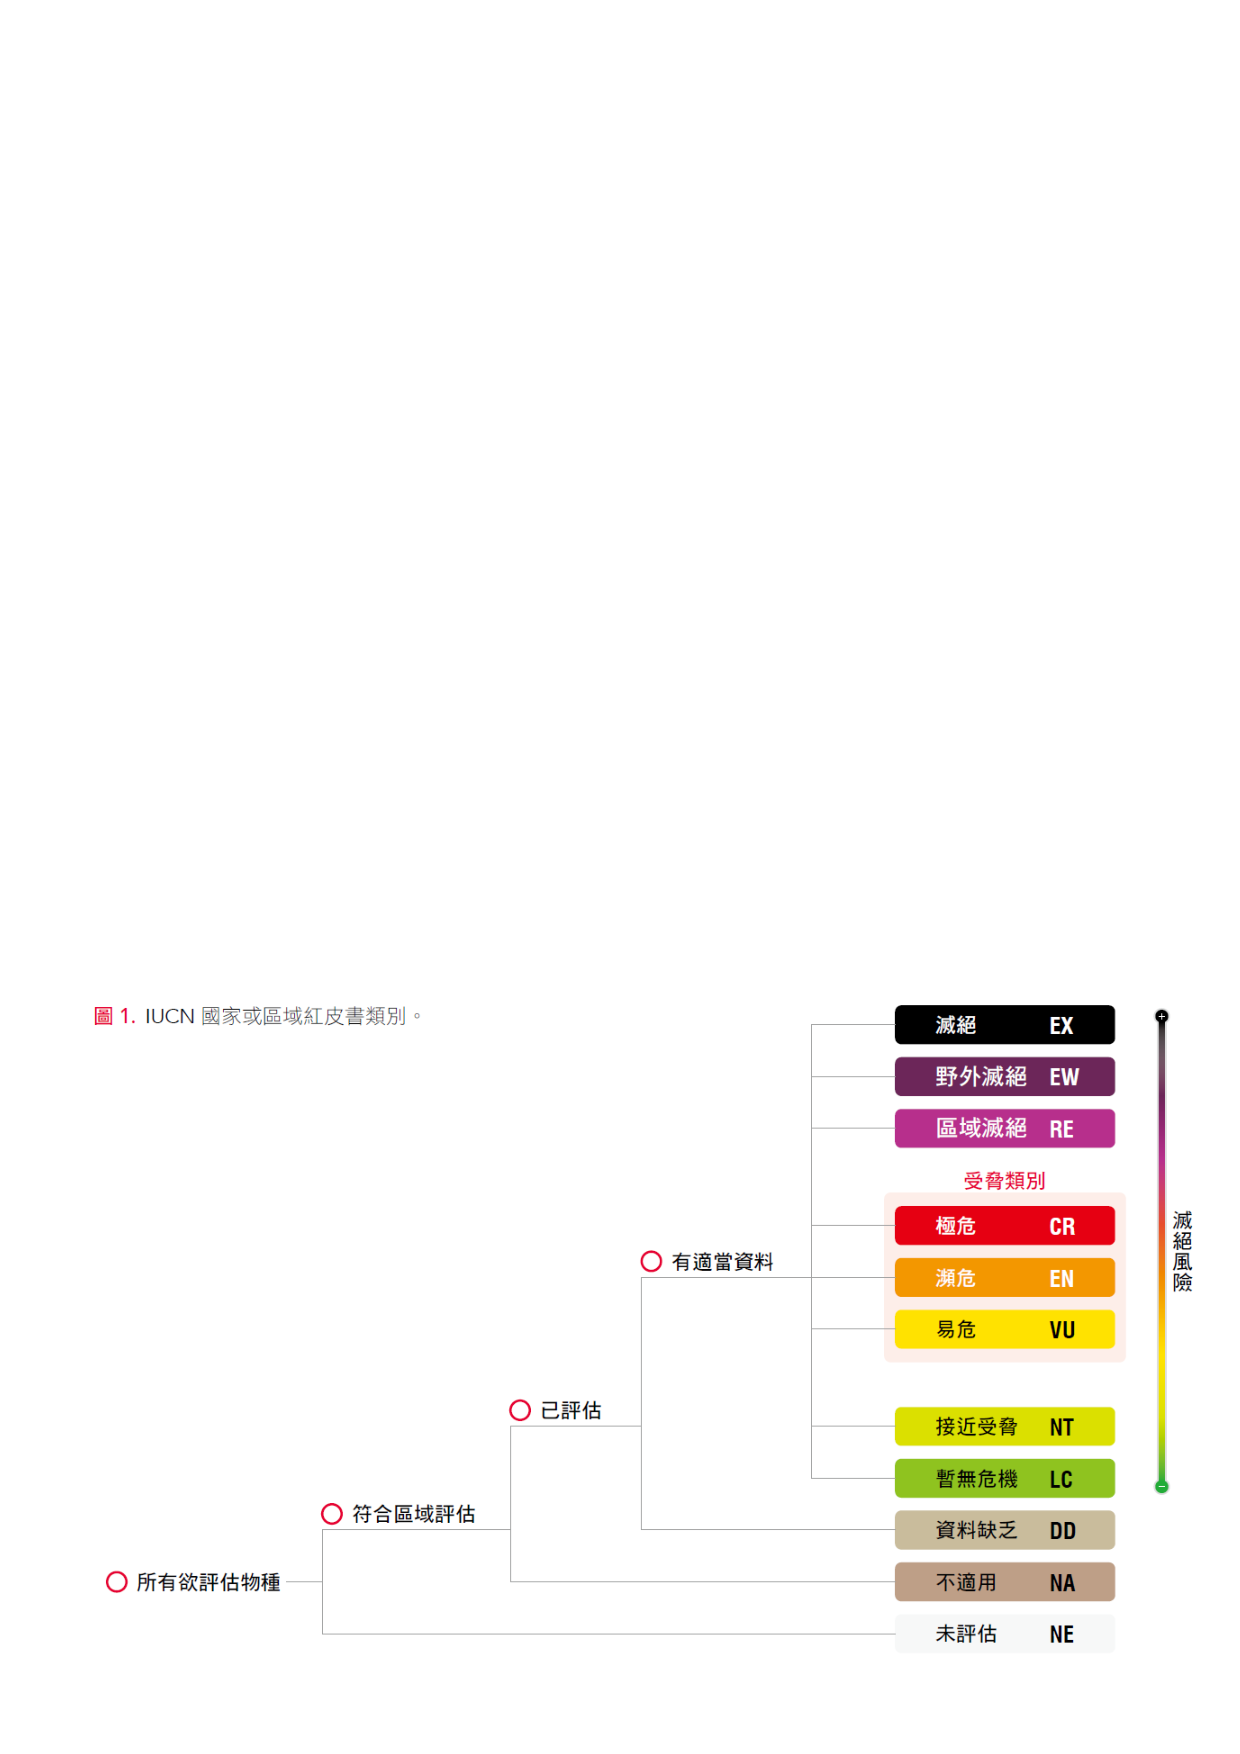
\includegraphics[width=\textwidth]{fig1.pdf}
\end{figure}
\begin{multicols}{2}
IUCN 紅皮書原是以全球做為評估範圍的, 如果一個地區、國家或地方性的紅皮書的產生是依據 IUCN 系統,
那麼就必須無偏差地根據 IUCN 紅皮書類別及標準(IUCN Red List Catego- ries and Criteria)進行評估(IUCN 2012b);
但由全球轉至地區(包括地區、國家及地方)進行評估時,對受威脅物種而言,自然會產生原生或外來種,
繁殖或非繁殖物種,或如先前曾經分布,但已局部滅絕的區域現象(IUCN 2012a)。
也就是說,由於空間尺度的關係,當全球的標準應用於分布不完全侷限於評估範圍的物種時,
評估流程與標準設定的閥值可能並不適當,因此必須有所有調整,
IUCN 從 1999 年開始對於紅皮書名錄地區及國家級評估標準應用指南提供調整建議(Gärdenfors 1999 ; IUCN 2012a)。
本報告採用的評估標準與類別係依據 IUCN 紅皮書名錄類別與標準: 3.1 版(IUCN 2012b),
並以地區及國家階層的應用指引: 4.0 版(IUCN 2012a)進行調整。
全球植物紅皮書現有的主要清單(Old eld et al. 1998; Walter and Gille  1998),
由於不是以現今的標準進行評估,因此絕大部分不能使用,僅有蘇鐵類及松柏類植物可以使用;
少數分類群雖使用修改過後的標準進行全球的物種 評估(Cicuzza et al. 2007 ; Gibbs and Chen
2009 ; Gibbs et al. 2011 ; Oldfield and Eastwood 2007),
但這些紅皮書中亦指出內中有不少的分類爭議及資訊不足之處,
尤以臺灣的物種多是以 Flora of China 為基礎進行評估,
分類及評估標準爭議更是明顯,更需要從區域進行標準化的評估,保育類別的資訊方能更為精準。\\

臺灣的自生維管束植物超過五千種,其中 約有四分之ㄧ為特有種,
豐富之植物種類實為國家重要的資源,然近年來環境破壞日益加劇,
頗多物種已面臨滅絕的危機,特有生物研 究保育中心與臺灣植物分類學會於 97 至 99 年度合作,
使用 IUCN 紅皮書類別及標準進行臺 灣地區野生維管束植物的物種存活受威脅程度評估─
「建構全國生物物種多樣性指標系統─ 植物紅皮書編纂及出版」,累計三年共完成 4,174 種之評估,
其中屬於受威脅(包括嚴重瀕臨絕滅、瀕臨絕滅及易受害)之物種共 908 種,
並出版「臺灣維管束植物紅皮書初評名錄」(王 震哲等,2012)。然自該計畫結束後,
植物學者陸續發表之臺灣新種或新紀錄種達 300 種以 上,
而許多原受評為受威脅物種者此期間亦新增諸多族群資訊與分類資料,需予以重新評估審定。
本報告蒐集及更新臺灣所有自生維管束植物的分布範圍、族群趨勢、數量與受脅原因等資訊,
依據 IUCN 類別與標準評估各植物。\\
\end{multicols}

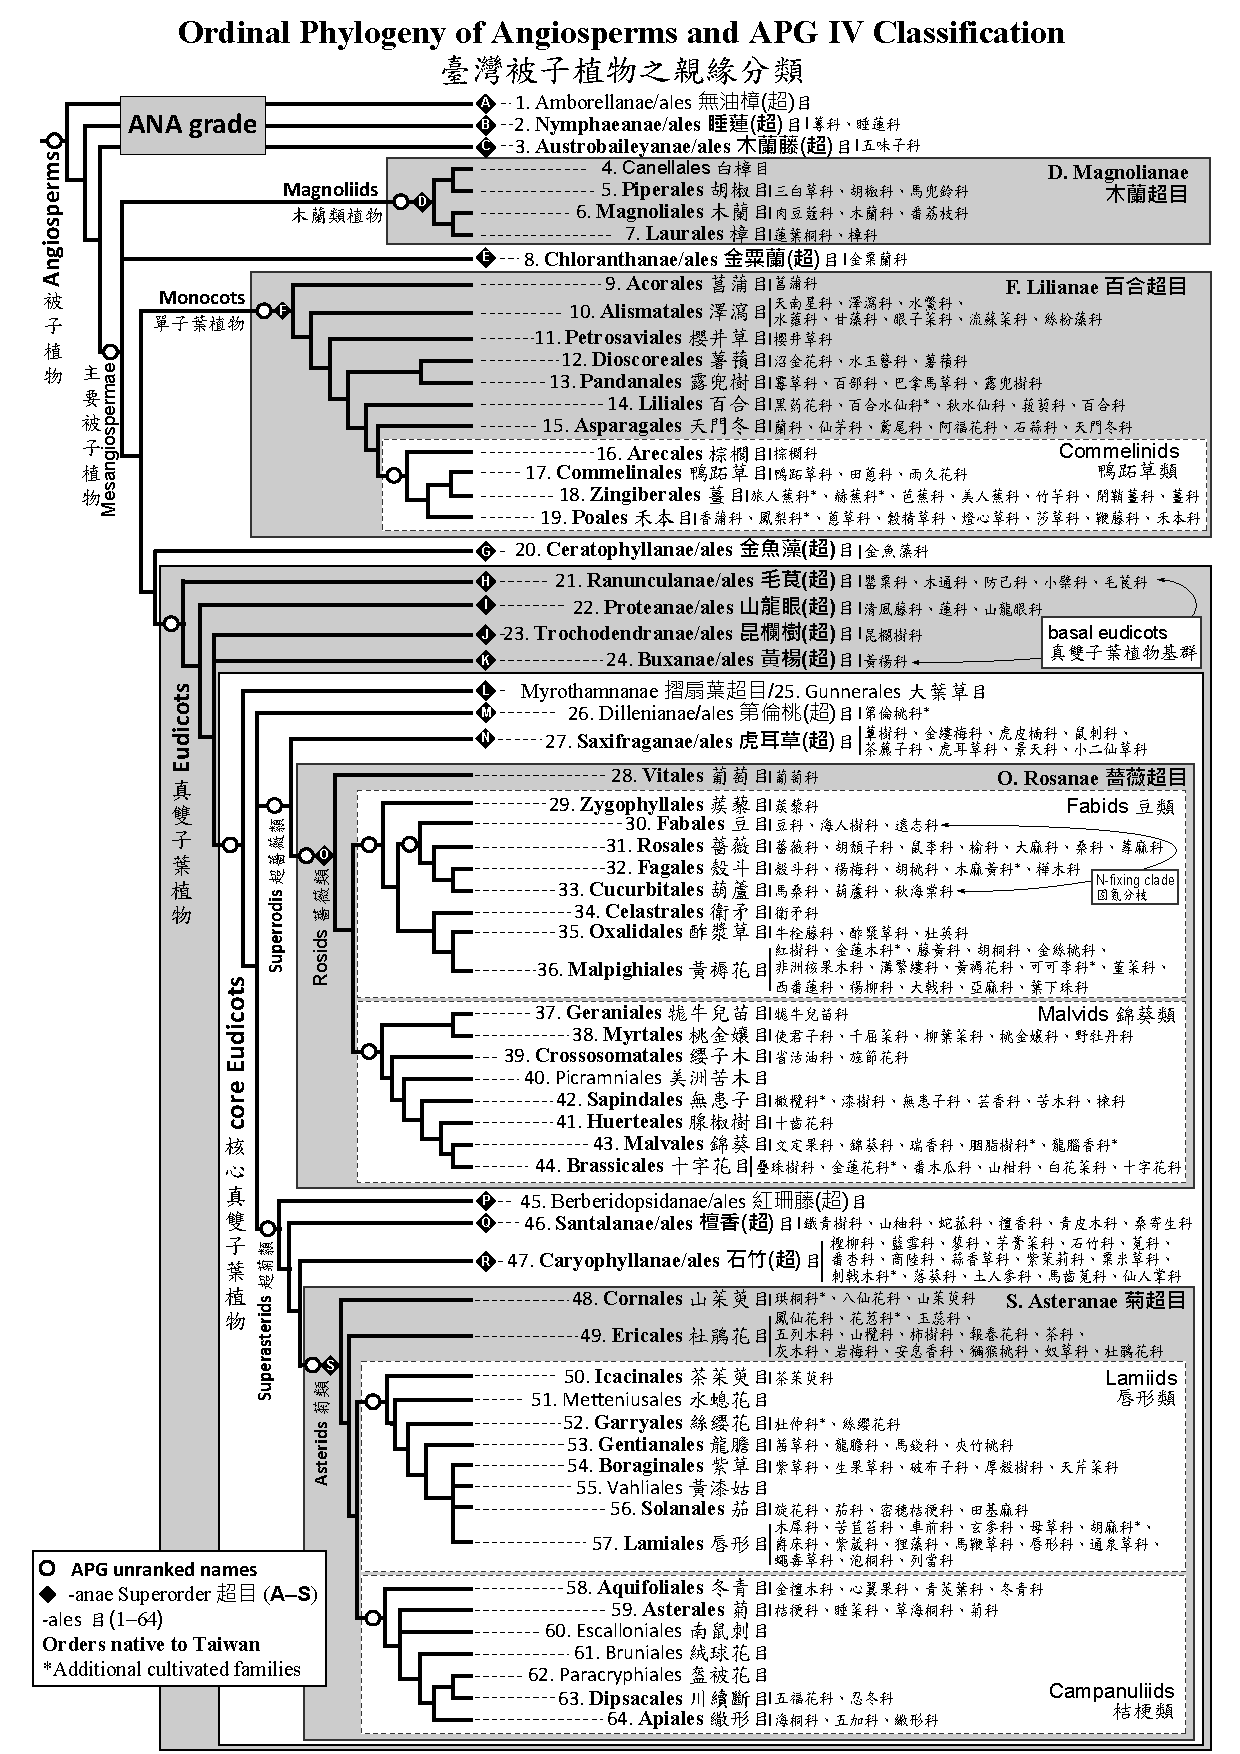
\includepdf{APGIV.pdf}

    \chapter{評估流程}

\begin{multicols}{2}
本報告採用的評估準則與類別係依據 IUCN 紅皮書名錄類別與標準:3.1版(IUCN 2012b)
及IUCN紅皮書名錄地區及國家級評估標準應用指南:4.0版(IUCN 2012a),
並參照 IUCN 紅皮書名錄類別與標準應用指南(IUCN Standards and Petitions Subcommittee 2017),
考慮了原生或外來種的問題,對臺灣野生維管束植物進行紅皮書評估。其評估流程與方法簡述如下:
\end{multicols}
\section{界定納入評估之分類群}
\begin{multicols}{2}
本報告評估的範圍為臺灣本島及附屬島嶼(彭佳嶼、棉花嶼、花瓶嶼、基隆嶼、澎湖群島、
小琉球、龜山島、綠島、蘭嶼及小蘭嶼)的野生維管束植物物種,但不包括鄰近中國大陸的
金門和馬祖以及東沙和南沙群島。評估的分類單元原則為「種」,但範圍內同時有亞種或變種出現時則分別評估,
原則上不包括變種以下階級、雜交種及外來種。以「臺灣維管束植物紅皮書初評名錄」(王震哲等 2012)
評估結果所收集的物種為基礎,
加上 2017 年 6 月 30 日前發表的新種與新紀錄種,以及初評時遺漏的物種,
共有 5188 種野生維管束植物列入候選評估名單。
其次依據IUCN紅皮書名錄地區及國家級評估標準應用指南(IUCN 2012a)的建議流程,
排除不適用(Not Applicable, NA)於區域評估的物種,
其餘分布於臺灣本島及附屬島嶼涵蓋範圍內之野生維管束植物均列入正式評估清單,
共 4442 種進入評估流程。 \\
\end{multicols}
\section{資訊收集與初步評估}
\begin{multicols}{2}

完成並確認候選評估名單後,由編輯委員會送請相關的專家進行評估。
依據標準為IUCN紅皮書名錄類別與標準:3.1版(IUCN 2012b) 與 IUCN
地區及國家級評估標準應用指南:4.0版(IUCN 2012a)。
每一受評分類群均依照IUCN紅皮書名錄類別與標準使用指南:
13版進行評估(IUCN Standards and Petitions Subcommittee 2017),得出初步類別。
評估流程係由包括:A. 快速族群下降(Rapid population reduction)、
B. 分布侷限、碎裂化,同時存在族群下降或嚴重波動(Small range and fragmented, declining, or extreme fluctuations)、
C. 小族群且持續下降(Small population and declining)、D. 非常小的族群(Very small population)、
E. 量化分析(Quantitative analysis)等五大標準及對應之次要標準(Sub-criterion)及資格限制(Qualifiers)
所構成之決策樹(logic tree)進行(表\ref{table1})。每個分類單元都會依所有標準進行評估,
只要符合任一條標準者,即列入受脅物種的類別,並在文件報告中列出符合類別的標準及對應之次標準。
某一物種經過評估後,無法符合國家極危(Nationally Critically Endangered, NCR)、
國家瀕危(Nationally Endangered, NEN)及國家易危(Nationally Vulnerable, NVU)的類別,
但已很接近或未來可能達到國家易危類別時,可列入國家接近受脅(Nationally Near-threatened, NNT)。
由於IUCN紅皮書名錄類別與標準並無明確的接近受脅(NT)標準定義,
本報告根據前述原則設定本報告國家接近受脅的標準(表\ref{table1})。\\
\end{multicols}
\begin{table}[!ht]
\caption{IUCN 紅皮書受脅( 極危、瀕危、易危) 及接近受脅類別評估標準簡要內容。修正自 IUCN Standards and Petitions Subcommittee (2017)} \label{table1}
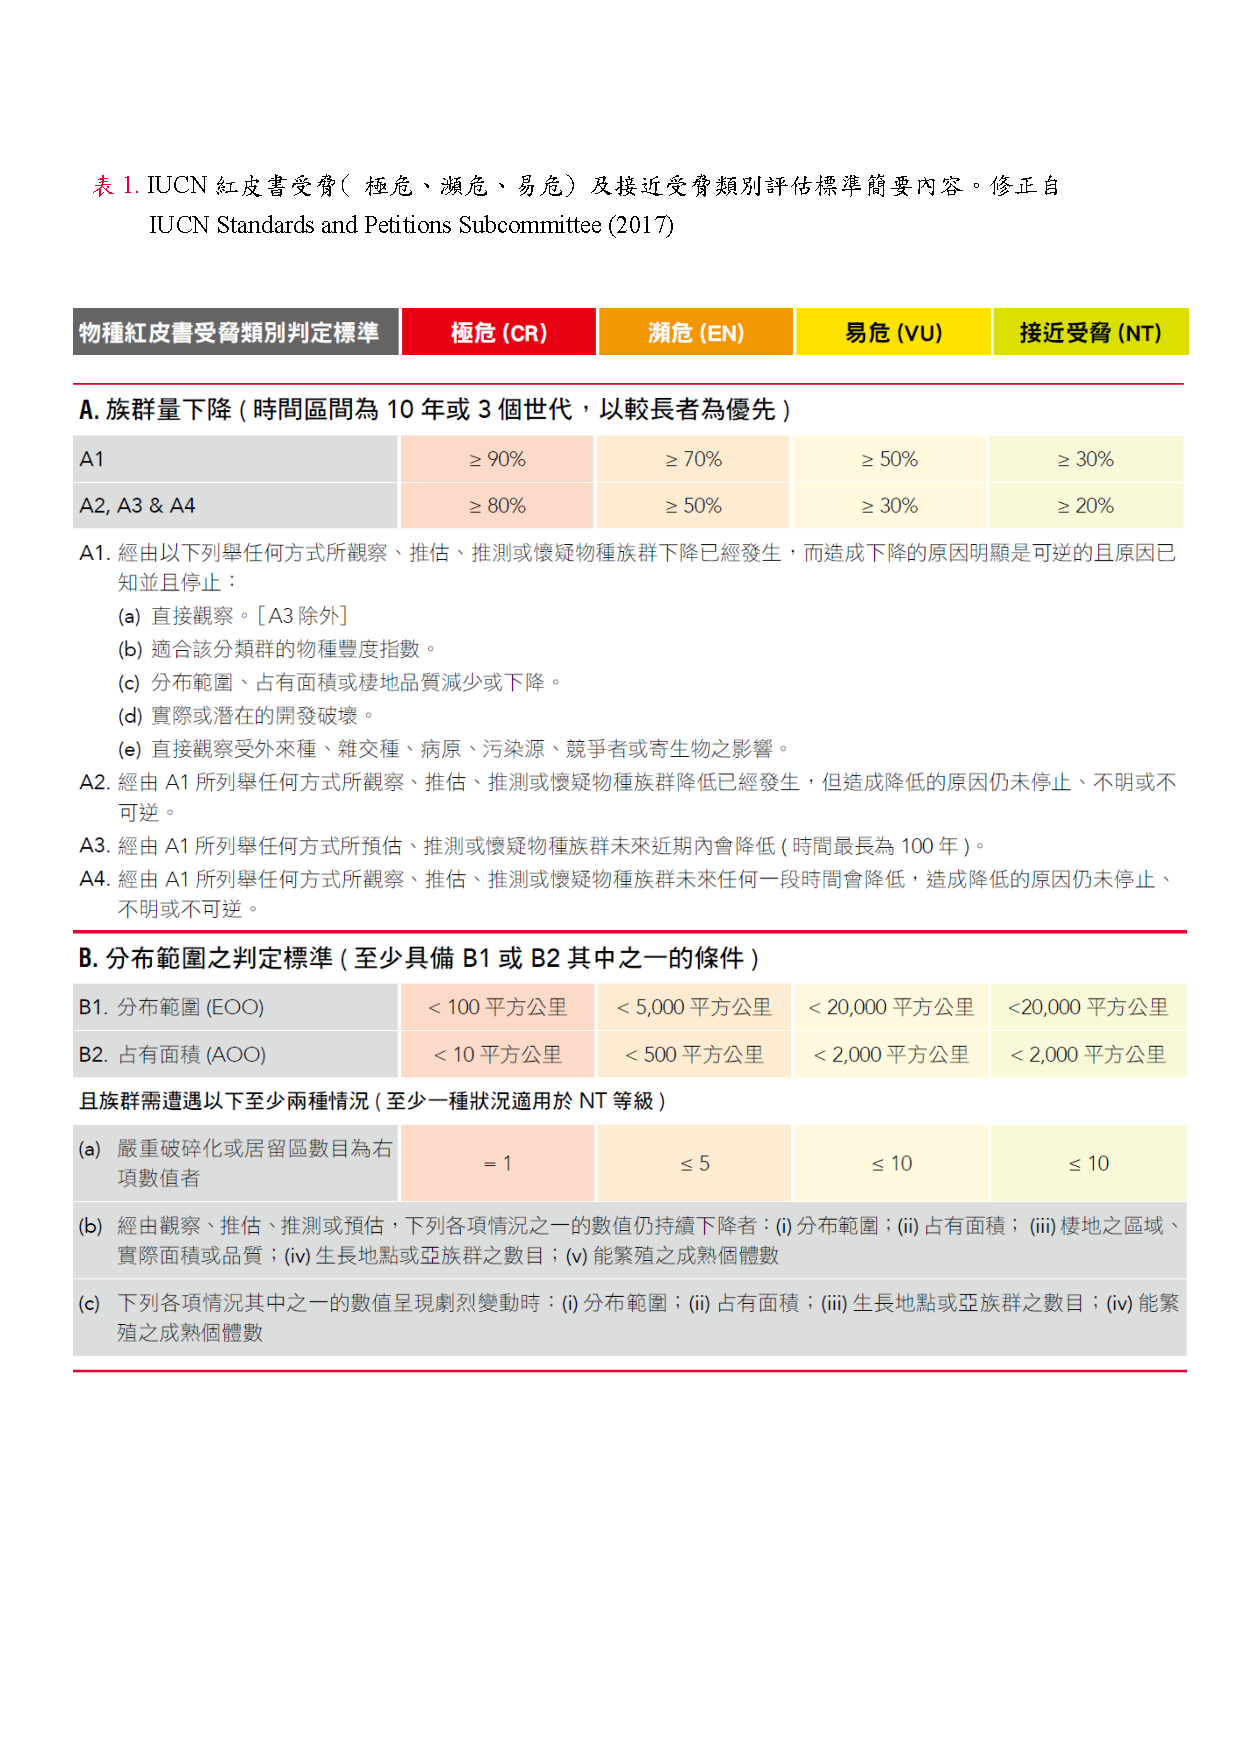
\includegraphics[scale=0.9]{iucn_standards.pdf}
\end{table}
\begin{figure}[!ht]
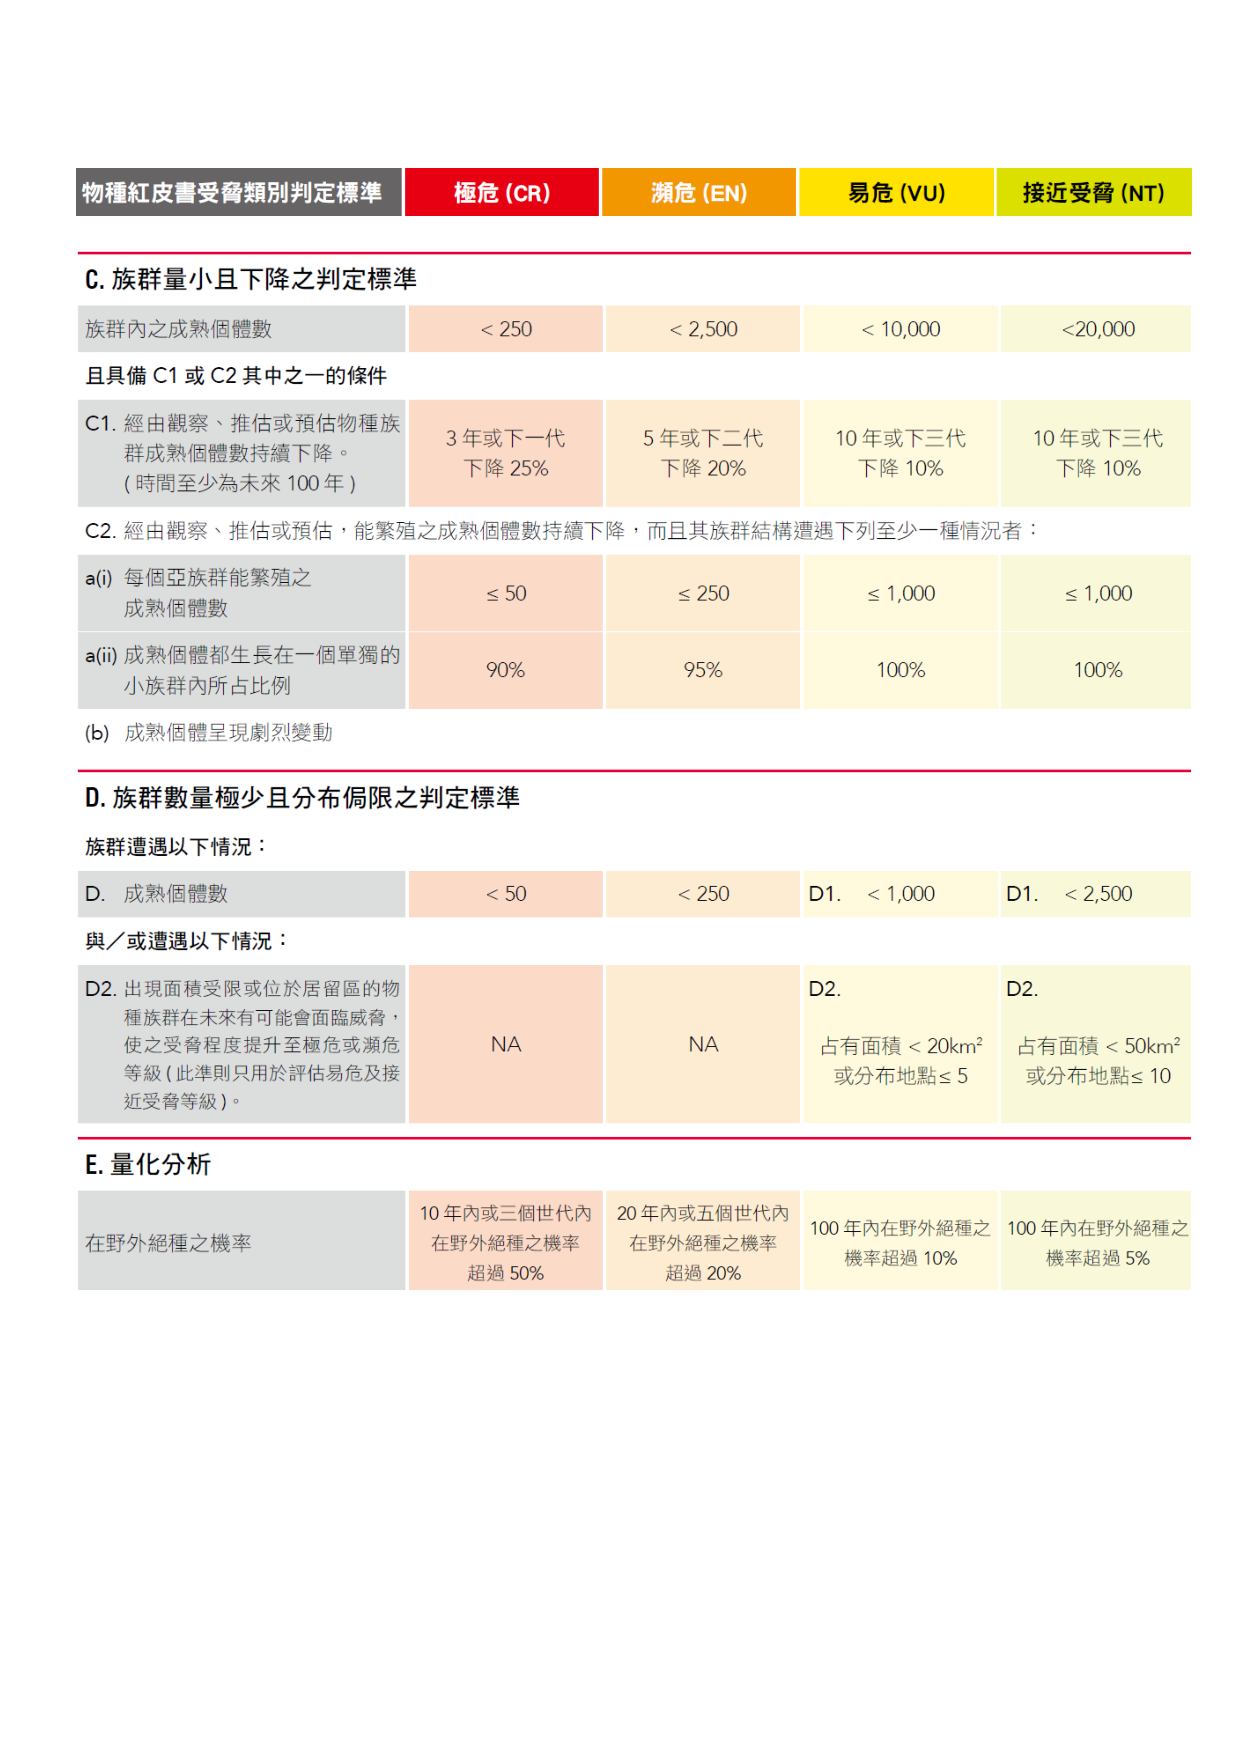
\includegraphics[scale=0.9]{iucn_standards2.pdf}
\end{figure}
\clearpage
\section{類別調整}
\begin{multicols}{2}
依據物種族群資料完成初步類別評估後,如果該物種非臺灣特有
需進一步考慮受評物種的區域滅絕機率受到評估範圍外相同分類群其他族群的影響程度(IUCN 2012a)
並依據評估結果將該物種的類別予以升級、降級或維持不變。
調整類別的原則依照IUCN(2012a)建議流程,而針對臺灣族群的調整標準說明如下:
\end{multicols}

\fbox{
    \begin{minipage}{0.9\textwidth}
\begin{enumerate}
    \item[1.] 若該分類群為臺灣特有,維持步驟 2.2 之評估類別結果。
    \item[2.] 若該分類群非臺灣特有,則再依下列原則進行評估,並依據評估結果將該分類群的類別予以升級、降級或維持不變:
    \begin{enumerate}
        \item[(1) ] 如果原分布地區或臺灣地區的棲息地環境有惡化現象,其類別保持不變。
        \item[(2) ] 如果在相鄰地區沒有同種族群或其繁殖體不能播遷到臺灣,臺灣族群可以視為本地特有的,其類別保持不變。
        \item[(3) ] 如果區外族群個體不可能在臺灣存活,類別保持不變。
        \item[(4) ] 如果沒有足夠的適宜棲息地或是現有保護措施不能在可預見的將來改善棲息地環境,區外的移入將不會降低絕滅危險,類別保持不變。
        \item[(5) ] 如果分類群在區外相對比較普遍,沒有族群衰退的跡象,且能夠播遷並有(或即將有)可利用的潛在棲息地,則降低其等級。如果分類群在相鄰地區正在減少,「救助影響」不容易發生,則提高類別。

        \item[(6) ] 如果有跡象表明一定數量的繁殖體定期到達該地而族群仍然只有少量存活,則地區族群可能為「數量衰減」。若是如此,繁殖體移入有即將停止的趨勢,提高類別。
    \end{enumerate}
\end{enumerate}
\end{minipage}
}

\section{公開意見徵詢}
\begin{multicols}{2}
經由步驟 2.1 至 2.3 產生的評估結果,
於 2017 年 6 月至 11 月徵求並彙整臺灣植物分類學會全體會員及全國相關機關
(如林試所、中研院生物多樣性中心、自然科學博物館等)、
團體及個人對於評定類別是否有所不當而需修改之意見,
並於 2017 年 12 月 1 日與林務局共同召開「臺灣維管束植物紅皮書成果說明會」,
廣泛徵求意見,最後再依據更新之資訊,再次執行 2.1 至 2.3 步驟後產生本報告。

\end{multicols}

    \linespread{0.8}\selectfont
    \chapter{臺灣維管束植物評估結果}

\phantomsection
\begin{Kai}

臺灣的野生維管束植物共 5,188 分類群,
其中 746 分類群不適用(Not Applicable)區域評估篩選條件,
4,442 分類群進入評估流程。評估的結果顯示臺灣有 27 種野生維管束植物已經滅絕,
其中 5 種屬於野外絕滅(Extinct in the Wild),22 種屬於區域滅絕(Regionally Extinct)。
國家受威脅(National Threatened)野生維管束植物共有 989 分類群,
其中屬於極危(Critically Endangered)類別有 195 分類群,
瀕危(Endangered)類別有 281 分類群,易危(Vulnerable)類別有 513 分類群。
另有 463 分類群歸於接近受脅(Near Threatened)的類別,335 分類群歸於資料缺乏(Data Deficient)的類別,
其餘 2628 分類群則屬於暫無危機(Least Concern)的類別。國家受威脅及接近受脅的野生維管束植物種數分別占評估種數的 22.3 \%及 10.4 \%。
所有納入評估候選的維管束植物的名單及其個別的保育類別亦另列一表,供作參考。

\linespread{1.5}\selectfont

\quad \\
\end{Kai}

\linespread{1}\selectfont
    \section{野外滅絕 (EW) 類別維管束植物名錄}
    \begin{footnotesize}
    %\begin{table}[!h]
    \begin{longtable}{p{3cm}p{2cm}p{5cm}p{3cm}}
    \toprule
      科名 & 科中名 & 分類群學名 & 分類群中名  \\
    \midrule 
    \endfirsthead
    
    {{\bfseries \tablename\ \thetable{} 續前頁 }} \\
    科名 & 科中名 & 分類群學名 & 分類群中名  \\
    \midrule
    \endhead
    Ericaceae & 杜鵑花科 & \textit{Rhododendron kanehirai}  & 烏來杜鵑\\
    Menyanthaceae & 睡菜科 & \textit{Nymphoides lungtanensis}  & 龍潭莕菜\\
    Musaceae & 芭蕉科 & \textit{Musa yamiensis}  & 雅美芭蕉\\
    Plantaginaceae & 車前科 & \textit{Limnophila taoyuanensis}  & 桃園石龍尾\\
    \bottomrule
    \end{longtable}
%%\end{table}
    \end{footnotesize}
    \section{區域滅絕 (RE) 類別維管束植物名錄}
    \begin{footnotesize}
    %\begin{table}[!h]
{\def\arraystretch{1.5}\tabcolsep=2pt
\begin{longtable}{p{3cm}p{2cm}p{5cm}p{3cm}}
    \toprule
      科名 & 科中名 & 分類群學名 & 分類群中名  \\
    \midrule
    \endfirsthead
    {{\bfseries \tablename\ \thetable{} 續前頁 }} \\
    科名 & 科中名 & 分類群學名 & 分類群中名  \\
    \midrule
    \endhead
    Asteraceae & 菊科 & \textit{Artemisia annua}  \index{Artemisia@\textit{Artemisia}!annua@\textit{annua}}               & 黃花蒿 \index{黃花蒿} \\
    Asteraceae & 菊科 & \textit{Tephroseris kirilowii}  \index{Tephroseris@\textit{Tephroseris}!kirilowii@\textit{kirilowii}}         & 狗舌草 \index{狗舌草} \\
    Cyperaceae & 莎草科 & \textit{Actinoscirpus grossus}  \index{Actinoscirpus@\textit{Actinoscirpus}!grossus@\textit{grossus}}       & 大藨草 \index{大藨草} \\
    Cyperaceae & 莎草科 & \textit{Carex metallica}  \index{Carex@\textit{Carex}!metallica@\textit{metallica}}             & 寬穗薹 \index{寬穗薹} \\
    Cyperaceae & 莎草科 & \textit{Carex scabrifolia}  \index{Carex@\textit{Carex}!scabrifolia@\textit{scabrifolia}}           & 鹼簣 \index{鹼簣} \\
    Cyperaceae & 莎草科 & \textit{Cyperus unioloides}  \index{Cyperus@\textit{Cyperus}!unioloides@\textit{unioloides}}          & 水社扁莎 \index{水社扁莎} \\
    Cyperaceae & 莎草科 & \textit{Fimbristylis acuminata}  \index{Fimbristylis@\textit{Fimbristylis}!acuminata@\textit{acuminata}}      & 尖穗飄拂草 \index{尖穗飄拂草} \\
    Cyperaceae & 莎草科 & \textit{Fimbristylis tetragona}  \index{Fimbristylis@\textit{Fimbristylis}!tetragona@\textit{tetragona}}      & 四方型飄拂草 \index{四方型飄拂草} \\
    Cyperaceae & 莎草科 & \textit{Rhynchospora chinensis}  \index{Rhynchospora@\textit{Rhynchospora}!chinensis@\textit{chinensis}}      & 華刺子莞 \index{華刺子莞} \\
    Cyperaceae & 莎草科 & \textit{Schoenus falcatus}  \index{Schoenus@\textit{Schoenus}!falcatus@\textit{falcatus}}           & 赤箭莎 \index{赤箭莎} \\
    Cyperaceae & 莎草科 & \textit{Scleria sumatrensis}  \index{Scleria@\textit{Scleria}!sumatrensis@\textit{sumatrensis}}         & 印尼珍珠茅 \index{印尼珍珠茅} \\
    Hydrocharitaceae & 水鱉科 & \textit{Najas ancistrocarpa}  \index{Najas@\textit{Najas}!ancistrocarpa@\textit{ancistrocarpa}}   & 彎果茨藻 \index{彎果茨藻} \\
    Lentibulariaceae & 狸藻科 & \textit{Utricularia uliginosa}  \index{Utricularia@\textit{Utricularia}!uliginosa@\textit{uliginosa}} & 齒萼挖耳草 \index{齒萼挖耳草} \\
    Linderniaceae & 母草科 & \textit{Lindernia nummularifolia}  \index{Lindernia@\textit{Lindernia}!nummularifolia@\textit{nummularifolia}} & 寬葉母草 \index{寬葉母草} \\
    Onagraceae & 柳葉菜科 & \textit{Circaea glabrescens}  \index{Circaea@\textit{Circaea}!glabrescens@\textit{glabrescens}}       & 禿梗露珠草 \index{禿梗露珠草} \\
    Orchidaceae & 蘭科 & \textit{Liparis ferruginea}  \index{Liparis@\textit{Liparis}!ferruginea@\textit{ferruginea}}           & 明潭羊耳蒜 \index{明潭羊耳蒜} \\
    Poaceae & 禾本科 & \textit{Hygroryza aristata}  \index{Hygroryza@\textit{Hygroryza}!aristata@\textit{aristata}}             & 水禾 \index{水禾} \\
    Poaceae & 禾本科 & \textit{Oryza rufipogon}  \index{Oryza@\textit{Oryza}!rufipogon@\textit{rufipogon}}                & 野生稻 \index{野生稻} \\
    Primulaceae & 報春花科 & \textit{Lysimachia candida}  \index{Lysimachia@\textit{Lysimachia}!candida@\textit{candida}}       & 澤珍珠菜 \index{澤珍珠菜} \\
    Rhizophoraceae & 紅樹科 & \textit{Bruguiera gymnorrhiza}  \index{Bruguiera@\textit{Bruguiera}!gymnorrhiza@\textit{gymnorrhiza}}   & 紅茄苳 \index{紅茄苳} \\
    Rhizophoraceae & 紅樹科 & \textit{Ceriops tagal}  \index{Ceriops@\textit{Ceriops}!tagal@\textit{tagal}}           & 細蕊紅樹 \index{細蕊紅樹} \\
    Rutaceae & 芸香科 & \textit{Zanthoxylum armatum}  \index{Zanthoxylum@\textit{Zanthoxylum}!armatum@\textit{armatum}}           & 秦椒 \index{秦椒} \\
    \bottomrule
    \end{longtable}
}
    \end{footnotesize}
    \section{國家極危 (NCR) 類別維管束植物名錄}
    \footnotesize\selectfont
%\begin{table}[!h]
        {\def\arraystretch{1.5}\tabcolsep=2pt
        \begin{longtable}{p{2.5cm}p{2cm}p{5cm}p{2.5cm}p{3cm}}
        \multicolumn{2}{l}{\large{Lycophytes 石松類植物}} & & \\
        & & & &\\
        \toprule
          \color{red}{\textbf{科名}} & \color{red}{\textbf{科中名}} & \color{red}{\textbf{分類群學名}} & \color{red}{\textbf{分類群中名}} & \color{red}{\textbf{評估標準}} \\
        \midrule 
        \endfirsthead

        \multicolumn{5}{l}{\large\color{red}{\Kai{國家極危 (NCR) 類別維管束植物名錄(續)}}} \\
        \toprule
        \color{red}{\textbf{科名}} & \color{red}{\textbf{科中名}} & \color{red}{\textbf{分類群學名}} & \color{red}{\textbf{分類群中名}} & \color{red}{\textbf{評估標準}} \\
        \midrule
        \endhead
                Isoëtaceae & 水韭科 & \href{http://www.theplantlist.org/tpl1.1/search?q=Isoëtes+taiwanensis}{\textit{Isoëtes taiwanensis} } & 臺灣水韭 & A1ace; B2ab(ii,iii) \index{Isoëtes@\textit{Isoëtes}!taiwanensis@\textit{taiwanensis}}  \index{臺灣水韭} \\
    Lycopodiaceae & 石松科 & \href{http://www.theplantlist.org/tpl1.1/search?q=Phlegmariurus+cunninghamioides}{\textit{Phlegmariurus cunninghamioides} } & 寬葉石松 & C2a(i); D \index{Phlegmariurus@\textit{Phlegmariurus}!cunninghamioides@\textit{cunninghamioides}}  \index{寬葉石松} \\
    \bottomrule
        \end{longtable}
    %%\end{table}
        }
    
\footnotesize\selectfont
%\begin{table}[!h]
        {\def\arraystretch{1.5}\tabcolsep=2pt
        \begin{longtable}{p{2.5cm}p{2cm}p{5cm}p{2.5cm}p{3cm}}
        \multicolumn{2}{l}{\large{Monilophytes 蕨類植物}} & & \\
        & & & &\\
        \toprule
          \color{red}{\textbf{科名}} & \color{red}{\textbf{科中名}} & \color{red}{\textbf{分類群學名}} & \color{red}{\textbf{分類群中名}} & \color{red}{\textbf{評估標準}} \\
        \midrule 
        \endfirsthead

        \multicolumn{5}{l}{\large\color{red}{\Kai{國家極危 (NCR) 類別維管束植物名錄(續)}}} \\
        \toprule
        \color{red}{\textbf{科名}} & \color{red}{\textbf{科中名}} & \color{red}{\textbf{分類群學名}} & \color{red}{\textbf{分類群中名}} & \color{red}{\textbf{評估標準}} \\
        \midrule
        \endhead
                Aspleniaceae & 鐵角蕨科 & \href{http://www.theplantlist.org/tpl1.1/search?q=Asplenium+crinicaule}{\textit{Asplenium crinicaule} } & 毛軸鐵角蕨 & B1ab(iii,v)c(iv)+2ab(iii,v)c(iv); C1+2a(ii)b; D \index{Asplenium@\textit{Asplenium}!crinicaule@\textit{crinicaule}}  \index{毛軸鐵角蕨} \\
    Blechnaceae & 烏毛蕨科 & \href{http://www.theplantlist.org/tpl1.1/search?q=Diploblechnum+fraseri}{\textit{Diploblechnum fraseri} } & 假桫欏 & C1+2a(ii) \index{Diploblechnum@\textit{Diploblechnum}!fraseri@\textit{fraseri}}  \index{假桫欏} \\
    Cystopteridaceae & 冷蕨科 & \href{http://www.theplantlist.org/tpl1.1/search?q=Gymnocarpium+oyamense}{\textit{Gymnocarpium oyamense} } & 羽節蕨 & C2a(i) \index{Gymnocarpium@\textit{Gymnocarpium}!oyamense@\textit{oyamense}}  \index{羽節蕨} \\
    Dennstaedtiaceae & 碗蕨科 & \href{http://www.theplantlist.org/tpl1.1/search?q=Microlepia+platyphylla}{\textit{Microlepia platyphylla} } & 闊葉鱗蓋蕨 & B1ab(ii,iii,iv)c(ii,iii,iv); C1+2a(ii)b; D \index{Microlepia@\textit{Microlepia}!platyphylla@\textit{platyphylla}}  \index{闊葉鱗蓋蕨} \\
    Dennstaedtiaceae & 碗蕨科 & \href{http://www.theplantlist.org/tpl1.1/search?q=Paesia+radula}{\textit{Paesia radula} } & 曲軸蕨 & D \index{Paesia@\textit{Paesia}!radula@\textit{radula}}  \index{曲軸蕨} \\
    Dryopteridaceae & 鱗毛蕨科 & \href{http://www.theplantlist.org/tpl1.1/search?q=Elaphoglossum+commutatum}{\textit{Elaphoglossum commutatum} } & 大葉舌蕨 & D \index{Elaphoglossum@\textit{Elaphoglossum}!commutatum@\textit{commutatum}}  \index{大葉舌蕨} \\
    Dryopteridaceae & 鱗毛蕨科 & \href{http://www.theplantlist.org/tpl1.1/search?q=Polystichum+attenuatum}{\textit{Polystichum attenuatum} } & 長羽芽苞耳蕨 & B1ab(iii,v)c(ii,iv)+2ab(iii,v)c(ii,iv); C1+2a(ii)b; D \index{Polystichum@\textit{Polystichum}!attenuatum@\textit{attenuatum}}  \index{長羽芽苞耳蕨} \\
    Dryopteridaceae & 鱗毛蕨科 & \href{http://www.theplantlist.org/tpl1.1/search?q=Polystichum+capillipes}{\textit{Polystichum capillipes} } & 小耳蕨 & C2a(i) \index{Polystichum@\textit{Polystichum}!capillipes@\textit{capillipes}}  \index{小耳蕨} \\
    Dryopteridaceae & 鱗毛蕨科 & \href{http://www.theplantlist.org/tpl1.1/search?q=Polystichum+chunii}{\textit{Polystichum chunii} } & 陳氏耳蕨 & B1ab(iii,v)c(ii,iv)+2ab(iii,v)c(ii,iv); C1+2a(ii)b; D \index{Polystichum@\textit{Polystichum}!chunii@\textit{chunii}}  \index{陳氏耳蕨} \\
    Dryopteridaceae & 鱗毛蕨科 & \href{http://www.theplantlist.org/tpl1.1/search?q=Polystichum+grandifrons}{\textit{Polystichum grandifrons} } & 九州耳蕨 & B1ab(iii,v)c(ii,iv)+2ab(iii,v)c(ii,iv); C1+2a(ii)b; D \index{Polystichum@\textit{Polystichum}!grandifrons@\textit{grandifrons}}  \index{九州耳蕨} \\
    Dryopteridaceae & 鱗毛蕨科 & \href{http://www.theplantlist.org/tpl1.1/search?q=Polystichum+herbaceum}{\textit{Polystichum herbaceum} } & 草葉耳蕨 & B1ab(iii,v)c(ii,iv)+2ab(iii,v)c(ii,iv); C1+2a(ii)b; D \index{Polystichum@\textit{Polystichum}!herbaceum@\textit{herbaceum}}  \index{草葉耳蕨} \\
    Dryopteridaceae & 鱗毛蕨科 & \href{http://www.theplantlist.org/tpl1.1/search?q=Polystichum+tenuius}{\textit{Polystichum tenuius} } & 離脈柳葉蕨 & A4cd; B1b(i,ii, iii, iv, v)c(ii,iii,iv)+2b(i,ii, iii,iv,v)c(ii,iii,iv) \index{Polystichum@\textit{Polystichum}!tenuius@\textit{tenuius}}  \index{離脈柳葉蕨} \\
    Hymenophyllaceae & 膜蕨科 & \href{http://www.theplantlist.org/tpl1.1/search?q=Crepidomanes+bipunctatum}{\textit{Crepidomanes bipunctatum} } & 南洋假脈蕨 & B1ab(iii)+2ab(iii); C1 \index{Crepidomanes@\textit{Crepidomanes}!bipunctatum@\textit{bipunctatum}}  \index{南洋假脈蕨} \\
    Hymenophyllaceae & 膜蕨科 & \href{http://www.theplantlist.org/tpl1.1/search?q=Crepidomanes+parvifolium}{\textit{Crepidomanes parvifolium} } & 小葉假脈蕨 & D \index{Crepidomanes@\textit{Crepidomanes}!parvifolium@\textit{parvifolium}}  \index{小葉假脈蕨} \\
    Hymenophyllaceae & 膜蕨科 & \href{http://www.theplantlist.org/tpl1.1/search?q=Hymenophyllum+palmatifidum}{\textit{Hymenophyllum palmatifidum} } & 毛緣細口團扇蕨 & D \index{Hymenophyllum@\textit{Hymenophyllum}!palmatifidum@\textit{palmatifidum}}  \index{毛緣細口團扇蕨} \\
    Hymenophyllaceae & 膜蕨科 & \href{http://www.theplantlist.org/tpl1.1/search?q=Hymenophyllum+productum}{\textit{Hymenophyllum productum} } & 南洋蕗蕨 & B2ab(iii) \index{Hymenophyllum@\textit{Hymenophyllum}!productum@\textit{productum}}  \index{南洋蕗蕨} \\
    Hymenophyllaceae & 膜蕨科 & \href{http://www.theplantlist.org/tpl1.1/search?q=Hymenophyllum+simonsianum}{\textit{Hymenophyllum simonsianum} } & 寬片膜蕨 & D \index{Hymenophyllum@\textit{Hymenophyllum}!simonsianum@\textit{simonsianum}}  \index{寬片膜蕨} \\
    Hymenophyllaceae & 膜蕨科 & \href{http://www.theplantlist.org/tpl1.1/search?q=Hymenophyllum+taiwanense}{\textit{Hymenophyllum taiwanense} } & 臺灣蕗蕨 & D \index{Hymenophyllum@\textit{Hymenophyllum}!taiwanense@\textit{taiwanense}}  \index{臺灣蕗蕨} \\
    Marattiaceae & 觀音座蓮舅科 & \href{http://www.theplantlist.org/tpl1.1/search?q=Ptisana+pellucida}{\textit{Ptisana pellucida} } & 觀音座蓮舅 & C2a(ii) \index{Ptisana@\textit{Ptisana}!pellucida@\textit{pellucida}}  \index{觀音座蓮舅} \\
    Onocleaceae & 球子蕨科 & \href{http://www.theplantlist.org/tpl1.1/search?q=Pentarhizidium+orientale}{\textit{Pentarhizidium orientale} } & 東方莢果蕨 & C2a(i) \index{Pentarhizidium@\textit{Pentarhizidium}!orientale@\textit{orientale}}  \index{東方莢果蕨} \\
    Ophioglossaceae & 瓶爾小草科 & \href{http://www.theplantlist.org/tpl1.1/search?q=Helminthostachys+zeylanica}{\textit{Helminthostachys zeylanica} } & 錫蘭七指蕨 & B2ab(iii) \index{Helminthostachys@\textit{Helminthostachys}!zeylanica@\textit{zeylanica}}  \index{錫蘭七指蕨} \\
    Plagiogyriaceae & 瘤足蕨科 & \href{http://www.theplantlist.org/tpl1.1/search?q=Plagiogyria+koidzumii}{\textit{Plagiogyria koidzumii} } & 小泉氏瘤足蕨 & C2a(i) \index{Plagiogyria@\textit{Plagiogyria}!koidzumii@\textit{koidzumii}}  \index{小泉氏瘤足蕨} \\
    Polypodiaceae & 水龍骨科 & \href{http://www.theplantlist.org/tpl1.1/search?q=Lepisorus+mucronatus}{\textit{Lepisorus mucronatus} } & 尖嘴蕨 & C2a(i) \index{Lepisorus@\textit{Lepisorus}!mucronatus@\textit{mucronatus}}  \index{尖嘴蕨} \\
    Polypodiaceae & 水龍骨科 & \href{http://www.theplantlist.org/tpl1.1/search?q=Oreogrammitis+marivelesensis}{\textit{Oreogrammitis marivelesensis} } & 弼昭禾葉蕨 & B1ab(iii)+2ab(iii); C2a(i,ii); D \index{Oreogrammitis@\textit{Oreogrammitis}!marivelesensis@\textit{marivelesensis}}  \index{弼昭禾葉蕨} \\
    Polypodiaceae & 水龍骨科 & \href{http://www.theplantlist.org/tpl1.1/search?q=Oreogrammitis+orientalis}{\textit{Oreogrammitis orientalis} } & 東亞禾葉蕨 & D \index{Oreogrammitis@\textit{Oreogrammitis}!orientalis@\textit{orientalis}}  \index{東亞禾葉蕨} \\
    Polypodiaceae & 水龍骨科 & \href{http://www.theplantlist.org/tpl1.1/search?q=Prosaptia+pectinata}{\textit{Prosaptia pectinata} } & 篦齒穴子蕨 & C2a(i) \index{Prosaptia@\textit{Prosaptia}!pectinata@\textit{pectinata}}  \index{篦齒穴子蕨} \\
    Polypodiaceae & 水龍骨科 & \href{http://www.theplantlist.org/tpl1.1/search?q=Radiogrammitis+ilanensis}{\textit{Radiogrammitis ilanensis} } & 宜蘭禾葉蕨 & C2a(i) \index{Radiogrammitis@\textit{Radiogrammitis}!ilanensis@\textit{ilanensis}}  \index{宜蘭禾葉蕨} \\
    Polypodiaceae & 水龍骨科 & \href{http://www.theplantlist.org/tpl1.1/search?q=Radiogrammitis+moorei}{\textit{Radiogrammitis moorei} } & 牟氏輻禾蕨 & B2ab(v); C2a(ii) \index{Radiogrammitis@\textit{Radiogrammitis}!moorei@\textit{moorei}}  \index{牟氏輻禾蕨} \\
    Polypodiaceae & 水龍骨科 & \href{http://www.theplantlist.org/tpl1.1/search?q=Xiphopterella+devolii}{\textit{Xiphopterella devolii} } & 劍羽蕨 & B2ab(iii) \index{Xiphopterella@\textit{Xiphopterella}!devolii@\textit{devolii}}  \index{劍羽蕨} \\
    Pteridaceae & 鳳尾蕨科 & \href{http://www.theplantlist.org/tpl1.1/search?q=Adiantum+capillus-junonis}{\textit{Adiantum capillus-junonis} } & 團羽鐵線蕨 & C2b \index{Adiantum@\textit{Adiantum}!capillus-junonis@\textit{capillus-junonis}}  \index{團羽鐵線蕨} \\
    Pteridaceae & 鳳尾蕨科 & \href{http://www.theplantlist.org/tpl1.1/search?q=Haplopteris+heterophylla}{\textit{Haplopteris heterophylla} } & 異葉書帶蕨 & B1bc; C2a(iii)b \index{Haplopteris@\textit{Haplopteris}!heterophylla@\textit{heterophylla}}  \index{異葉書帶蕨} \\
    Pteridaceae & 鳳尾蕨科 & \href{http://www.theplantlist.org/tpl1.1/search?q=Pteris+angustipinna}{\textit{Pteris angustipinna} } & 細葉鳳尾蕨 & C2a(i) \index{Pteris@\textit{Pteris}!angustipinna@\textit{angustipinna}}  \index{細葉鳳尾蕨} \\
    Pteridaceae & 鳳尾蕨科 & \href{http://www.theplantlist.org/tpl1.1/search?q=Pteris+dimorpha+var.+metagrevilleana}{\textit{Pteris dimorpha} var. \textit{metagrevilleana} } & 擬翅柄鳳尾蕨 & B2ac(ii); C2b; D \index{Pteris@\textit{Pteris}!dimorpha@\textit{dimorpha}!var. metagrevilleana@var. \textit{metagrevilleana}}  \index{擬翅柄鳳尾蕨} \\
    Pteridaceae & 鳳尾蕨科 & \href{http://www.theplantlist.org/tpl1.1/search?q=Pteris+wulaiensis}{\textit{Pteris wulaiensis} } & 烏來鳳尾蕨 & C2a(i); D \index{Pteris@\textit{Pteris}!wulaiensis@\textit{wulaiensis}}  \index{烏來鳳尾蕨} \\
    Pteridaceae & 鳳尾蕨科 & \href{http://www.theplantlist.org/tpl1.1/search?q=Vaginularia+trichoidea}{\textit{Vaginularia trichoidea} } & 一條線蕨 & B1b(ii,iii)c(ii,iv)+2b(ii,iii)c(ii,iv); C2b; D \index{Vaginularia@\textit{Vaginularia}!trichoidea@\textit{trichoidea}}  \index{一條線蕨} \\
    Salviniaceae & 槐葉蘋科 & \href{http://www.theplantlist.org/tpl1.1/search?q=Salvinia+natans}{\textit{Salvinia natans} } & 槐葉蘋 & A2c \index{Salvinia@\textit{Salvinia}!natans@\textit{natans}}  \index{槐葉蘋} \\
    Schizaeaceae & 莎草蕨科 & \href{http://www.theplantlist.org/tpl1.1/search?q=Schizaea+dichotoma}{\textit{Schizaea dichotoma} } & 分枝莎草蕨 & B2ab(i,iv); C2a(i) \index{Schizaea@\textit{Schizaea}!dichotoma@\textit{dichotoma}}  \index{分枝莎草蕨} \\
    Thelypteridaceae & 金星蕨科 & \href{http://www.theplantlist.org/tpl1.1/search?q=Metathelypteris+flaccida}{\textit{Metathelypteris flaccida} } & 薄葉凸軸蕨 & B1ac(ii,iii,iv)+2ac(ii,iii,iv) \index{Metathelypteris@\textit{Metathelypteris}!flaccida@\textit{flaccida}}  \index{薄葉凸軸蕨} \\
    Woodsiaceae & 岩蕨科 & \href{http://www.theplantlist.org/tpl1.1/search?q=Woodsia+andersonii}{\textit{Woodsia andersonii} } & 蜘蛛岩蕨 & B1ab(v)+2ab(v); D \index{Woodsia@\textit{Woodsia}!andersonii@\textit{andersonii}}  \index{蜘蛛岩蕨} \\
    Woodsiaceae & 岩蕨科 & \href{http://www.theplantlist.org/tpl1.1/search?q=Woodsia+okamotoi}{\textit{Woodsia okamotoi} } & 岡本氏岩蕨 & C2a(i) \index{Woodsia@\textit{Woodsia}!okamotoi@\textit{okamotoi}}  \index{岡本氏岩蕨} \\
    \bottomrule
        \end{longtable}
    %%\end{table}
        }
    
\noindent\normalfont\selectfont Gymnosperms 裸子植物
\footnotesize\selectfont
%\begin{table}[!h]
        {\def\arraystretch{1.5}\tabcolsep=2pt
        \begin{longtable}{p{2.5cm}p{2.5cm}p{4.5cm}p{2.5cm}p{3cm}}
        \toprule
          科名 & 科中名 & 分類群學名 & 分類群中名 & 評估標準 \\
        \midrule 
        \endfirsthead

        {{\bfseries 續前頁 }} \\
        科名 & 科中名 & 分類群學名 & 分類群中名 & 評估標準 \\
        \midrule
        \endhead
                Cycadaceae & 蘇鐵科 & \textit{Cycas taitungensis}  & 臺東蘇鐵 & B2b(i,ii,v) \index{Cycas@\textit{Cycas}!taitungensis@\textit{taitungensis}}  \index{臺東蘇鐵} \\
    Pinaceae & 松科 & \textit{Keteleeria davidiana} var. \textit{formosana}  & 臺灣油杉 & B2b(ii,v) \index{Keteleeria@\textit{Keteleeria}!davidiana@\textit{davidiana}!var. formosana@var. \textit{formosana}}  \index{臺灣油杉} \\
    Podocarpaceae & 羅漢松科 & \textit{Podocarpus costalis}  & 蘭嶼羅漢松 & A1ad; B2ab(ii,iii); D1 \index{Podocarpus@\textit{Podocarpus}!costalis@\textit{costalis}}  \index{蘭嶼羅漢松} \\
    \bottomrule
        \end{longtable}
    %%\end{table}
        }
    
\noindent\normalfont\selectfont Angiosperms 被子植物
\footnotesize\selectfont
%\begin{table}[!h]
        {\def\arraystretch{1.5}\tabcolsep=2pt
        \begin{longtable}{p{2.5cm}p{2.5cm}p{4.5cm}p{2.5cm}p{3cm}}
        \toprule
          科名 & 科中名 & 分類群學名 & 分類群中名 & 評估標準 \\
        \midrule 
        \endfirsthead

        {{\bfseries 續前頁 }} \\
        科名 & 科中名 & 分類群學名 & 分類群中名 & 評估標準 \\
        \midrule
        \endhead
                Alismataceae & 澤瀉科 & \textit{Caldesia grandis}  & 圓葉澤瀉 & B1ab(iii,v)+2ab(iii,v); C1+2a(i,ii); D \index{Caldesia@\textit{Caldesia}!grandis@\textit{grandis}}  \index{圓葉澤瀉} \\
    Annonaceae & 番荔枝科 & \textit{Goniothalamus amuyon}  & 恆春哥納香 & B2b(iv)c(iv); C2b \index{Goniothalamus@\textit{Goniothalamus}!amuyon@\textit{amuyon}}  \index{恆春哥納香} \\
    Annonaceae & 番荔枝科 & \textit{Polyalthia liukiuensis}  & 琉球暗羅 & B1ab(ii,v); C1 \index{Polyalthia@\textit{Polyalthia}!liukiuensis@\textit{liukiuensis}}  \index{琉球暗羅} \\
    Apiaceae & 繖形科 & \textit{Sium suave}  & 細葉零餘子 & D \index{Sium@\textit{Sium}!suave@\textit{suave}}  \index{細葉零餘子} \\
    Apocynaceae & 夾竹桃科 & \textit{Telosma pallida}  & 夜香花 & B2ab(ii) \index{Telosma@\textit{Telosma}!pallida@\textit{pallida}}  \index{夜香花} \\
    Aponogetonaceae & 水蕹科 & \textit{Aponogeton taiwanensis}  & 水蕹 & A2cd \index{Aponogeton@\textit{Aponogeton}!taiwanensis@\textit{taiwanensis}}  \index{水蕹} \\
    Araceae & 天南星科 & \textit{Lemna trisulca}  & 品藻 & A2ac; B2b(iii, iv)c(ii, iii) \index{Lemna@\textit{Lemna}!trisulca@\textit{trisulca}}  \index{品藻} \\
    Aristolochiaceae & 馬兜鈴科 & \textit{Aristolochia yujungiana}  & 裕榮馬兜鈴 & B1ab(iii,v); D \index{Aristolochia@\textit{Aristolochia}!yujungiana@\textit{yujungiana}}  \index{裕榮馬兜鈴} \\
    Aristolochiaceae & 馬兜鈴科 & \textit{Asarum tawushanianum}  & 大武山細辛 & B2ab(ii, iii, v) \index{Asarum@\textit{Asarum}!tawushanianum@\textit{tawushanianum}}  \index{大武山細辛} \\
    Asparagaceae & 天門冬科 & \textit{Thysanotus chinensis}  & 異蕊草 & B1 ab(i, iii, iv) \index{Thysanotus@\textit{Thysanotus}!chinensis@\textit{chinensis}}  \index{異蕊草} \\
    Asteraceae & 菊科 & \textit{Dendranthema horaimontana}  & 蓬萊油菊 & A2c \index{Dendranthema@\textit{Dendranthema}!horaimontana@\textit{horaimontana}}  \index{蓬萊油菊} \\
    Asteraceae & 菊科 & \textit{Echinops grijsii}  & 漏盧 & C2a(i, ii) \index{Echinops@\textit{Echinops}!grijsii@\textit{grijsii}}  \index{漏盧} \\
    Asteraceae & 菊科 & \textit{Gerbera anandria}  & 大丁草 & D \index{Gerbera@\textit{Gerbera}!anandria@\textit{anandria}}  \index{大丁草} \\
    Asteraceae & 菊科 & \textit{Syneilesis intermedia}  & 臺灣破傘菊 & B1+2abcde; D1+2 \index{Syneilesis@\textit{Syneilesis}!intermedia@\textit{intermedia}}  \index{臺灣破傘菊} \\
    Balanophoraceae & 蛇菰科 & \textit{Balanophora japonica}  & 日本蛇菰 & B2ac; C2a; D1 \index{Balanophora@\textit{Balanophora}!japonica@\textit{japonica}}  \index{日本蛇菰} \\
    Berberidaceae & 小檗科 & \textit{Berberis chingshuiensis}  & 清水山小檗 & B1ac(iv) \index{Berberis@\textit{Berberis}!chingshuiensis@\textit{chingshuiensis}}  \index{清水山小檗} \\
    Berberidaceae & 小檗科 & \textit{Berberis mingetsuensis}  & 眠月小檗 & B1ac(ii,iii) \index{Berberis@\textit{Berberis}!mingetsuensis@\textit{mingetsuensis}}  \index{眠月小檗} \\
    Berberidaceae & 小檗科 & \textit{Berberis tarokoensis}  & 太魯閣小檗 & B1ac(iv) \index{Berberis@\textit{Berberis}!tarokoensis@\textit{tarokoensis}}  \index{太魯閣小檗} \\
    Burmanniaceae & 水玉簪科 & \textit{Thismia taiwanensis}  & 臺灣水玉杯 & D \index{Thismia@\textit{Thismia}!taiwanensis@\textit{taiwanensis}}  \index{臺灣水玉杯} \\
    Capparaceae & 山柑科 & \textit{Capparis lanceolaris}  & 蘭嶼山柑 & B1ab(ii,v); C1 \index{Capparis@\textit{Capparis}!lanceolaris@\textit{lanceolaris}}  \index{蘭嶼山柑} \\
    Celastraceae & 衛矛科 & \textit{Euonymus huangii}  & 黃氏衛矛 & B1b(iii)c(iii) \index{Euonymus@\textit{Euonymus}!huangii@\textit{huangii}}  \index{黃氏衛矛} \\
    Celastraceae & 衛矛科 & \textit{Euonymus japonicus}  & 日本衛矛 & B2b(iv)c(iv); C2b \index{Euonymus@\textit{Euonymus}!japonicus@\textit{japonicus}}  \index{日本衛矛} \\
    Convolvulaceae & 旋花科 & \textit{Argyreia akoensis}  & 屏東朝顏 & B1a+2a; D1; D \index{Argyreia@\textit{Argyreia}!akoensis@\textit{akoensis}}  \index{屏東朝顏} \\
    Convolvulaceae & 旋花科 & \textit{Lepistemon intermedius}  & 光滑鮮蕊藤 & D \index{Lepistemon@\textit{Lepistemon}!intermedius@\textit{intermedius}}  \index{光滑鮮蕊藤} \\
    Convolvulaceae & 旋花科 & \textit{Merremia similis}  & 紅花姬旋花 & D \index{Merremia@\textit{Merremia}!similis@\textit{similis}}  \index{紅花姬旋花} \\
    Cyperaceae & 莎草科 & \textit{Carex kobomugi}  & 海米 & B1ab(iii,iv,v)+2ab(iii,iv,v); C1; D1 \index{Carex@\textit{Carex}!kobomugi@\textit{kobomugi}}  \index{海米} \\
    Cyperaceae & 莎草科 & \textit{Cyperus albescens}  & 華湖瓜草 & D1 \index{Cyperus@\textit{Cyperus}!albescens@\textit{albescens}}  \index{華湖瓜草} \\
    Cyperaceae & 莎草科 & \textit{Cyperus leptocarpus}  & 銀穗湖瓜草 & B1ab(i,ii,iii,iv,v)+2ab(i,ii,iii,iv,v) \index{Cyperus@\textit{Cyperus}!leptocarpus@\textit{leptocarpus}}  \index{銀穗湖瓜草} \\
    Cyperaceae & 莎草科 & \textit{Eleocharis retroflexa}  & 貝殼葉荸薺 & B1ab(iii) \index{Eleocharis@\textit{Eleocharis}!retroflexa@\textit{retroflexa}}  \index{貝殼葉荸薺} \\
    Cyperaceae & 莎草科 & \textit{Fimbristylis autumnalis}  & 秋飄拂草 & C1 \index{Fimbristylis@\textit{Fimbristylis}!autumnalis@\textit{autumnalis}}  \index{秋飄拂草} \\
    Cyperaceae & 莎草科 & \textit{Fimbristylis nutans}  & 點頭飄拂草 & D1 \index{Fimbristylis@\textit{Fimbristylis}!nutans@\textit{nutans}}  \index{點頭飄拂草} \\
    Cyperaceae & 莎草科 & \textit{Rhynchospora malasica}  & 馬來刺子莞 & A2d; D \index{Rhynchospora@\textit{Rhynchospora}!malasica@\textit{malasica}}  \index{馬來刺子莞} \\
    Dioscoreaceae & 薯蕷科 & \textit{Tacca leontopetaloides}  & 蒟蒻薯 & B1ab(iii,v) \index{Tacca@\textit{Tacca}!leontopetaloides@\textit{leontopetaloides}}  \index{蒟蒻薯} \\
    Elaeagnaceae & 胡頹子科 & \textit{Elaeagnus formosensis}  & 蓬萊胡頹子 & B1b(i,ii,iii,v)\&; D \index{Elaeagnus@\textit{Elaeagnus}!formosensis@\textit{formosensis}}  \index{蓬萊胡頹子} \\
    Eriocaulaceae & 穀精草科 & \textit{Eriocaulon nantoense}  & 南投穀精草 & B2ac(ii, iii) \index{Eriocaulon@\textit{Eriocaulon}!nantoense@\textit{nantoense}}  \index{南投穀精草} \\
    Eriocaulaceae & 穀精草科 & \textit{Eriocaulon nepalense}  & 尼泊爾穀精草 & B2ac(ii, iii) \index{Eriocaulon@\textit{Eriocaulon}!nepalense@\textit{nepalense}}  \index{尼泊爾穀精草} \\
    Eriocaulaceae & 穀精草科 & \textit{Eriocaulon taishanense}  & 泰山穀精草 & B2ac(ii, iv); D \index{Eriocaulon@\textit{Eriocaulon}!taishanense@\textit{taishanense}}  \index{泰山穀精草} \\
    Fabaceae & 豆科 & \textit{Hylodesmum densum}  & 菱葉山螞蝗 & B2ab(iii) \index{Hylodesmum@\textit{Hylodesmum}!densum@\textit{densum}}  \index{菱葉山螞蝗} \\
    Fabaceae & 豆科 & \textit{Indigofera byobiensis}  & 貓鼻頭木藍 & D1 \index{Indigofera@\textit{Indigofera}!byobiensis@\textit{byobiensis}}  \index{貓鼻頭木藍} \\
    Fabaceae & 豆科 & \textit{Indigofera taiwaniana}  & 臺灣木藍 & D \index{Indigofera@\textit{Indigofera}!taiwaniana@\textit{taiwaniana}}  \index{臺灣木藍} \\
    Fabaceae & 豆科 & \textit{Kummerowia stipulacea}  & 圓葉雞眼草 & B2ab(i, iii) \index{Kummerowia@\textit{Kummerowia}!stipulacea@\textit{stipulacea}}  \index{圓葉雞眼草} \\
    Fabaceae & 豆科 & \textit{Lespedeza daurica}  & 大胡枝子 & B2ab(i, iii) \index{Lespedeza@\textit{Lespedeza}!daurica@\textit{daurica}}  \index{大胡枝子} \\
    Fabaceae & 豆科 & \textit{Millettia pulchra} var. \textit{microphylla}  & 小葉魚藤 & D1 \index{Millettia@\textit{Millettia}!pulchra@\textit{pulchra}!var. microphylla@var. \textit{microphylla}}  \index{小葉魚藤} \\
    Fabaceae & 豆科 & \textit{Mucuna gigantea} subsp. \textit{tashiroi}  & 大血藤 & D1 \index{Mucuna@\textit{Mucuna}!gigantea@\textit{gigantea}!subsp. tashiroi@subsp. \textit{tashiroi}}  \index{大血藤} \\
    Fabaceae & 豆科 & \textit{Vigna adenantha}  & 腺葯豇豆 & B2ab(iii) \index{Vigna@\textit{Vigna}!adenantha@\textit{adenantha}}  \index{腺葯豇豆} \\
    Fagaceae & 殼斗科 & \textit{Lithocarpus formosanus}  & 臺灣石櫟 & D \index{Lithocarpus@\textit{Lithocarpus}!formosanus@\textit{formosanus}}  \index{臺灣石櫟} \\
    Fagaceae & 殼斗科 & \textit{Quercus aliena}  & 大槲樹 & B1ab(iii,v)+2ab(iii,v); C1 \index{Quercus@\textit{Quercus}!aliena@\textit{aliena}}  \index{大槲樹} \\
    Gentianaceae & 龍膽科 & \textit{Gentiana tarokoensis}  & 太魯閣龍膽 & B2ac(iii) \index{Gentiana@\textit{Gentiana}!tarokoensis@\textit{tarokoensis}}  \index{太魯閣龍膽} \\
    Gentianaceae & 龍膽科 & \textit{Gentiana tentyoensis}  & 厚葉龍膽 & B3ac(iii) \index{Gentiana@\textit{Gentiana}!tentyoensis@\textit{tentyoensis}}  \index{厚葉龍膽} \\
    Gentianaceae & 龍膽科 & \textit{Lomatogonium chilaiensis}  & 奇萊肋柱花 & B2ac(iii) \index{Lomatogonium@\textit{Lomatogonium}!chilaiensis@\textit{chilaiensis}}  \index{奇萊肋柱花} \\
    Gentianaceae & 龍膽科 & \textit{Tripterospermum lilungshanensis}  & 里龍山肺形草 & B2ac(iv) \index{Tripterospermum@\textit{Tripterospermum}!lilungshanensis@\textit{lilungshanensis}}  \index{里龍山肺形草} \\
    Goodeniaceae & 草海桐科 & \textit{Scaevola hainanensis}  & 海南草海桐 & B2ab(ii) \index{Scaevola@\textit{Scaevola}!hainanensis@\textit{hainanensis}}  \index{海南草海桐} \\
    Lamiaceae & 唇形科 & \textit{Lamium amplexicaule}  & 寶蓋草 & B2ab(v) \index{Lamium@\textit{Lamium}!amplexicaule@\textit{amplexicaule}}  \index{寶蓋草} \\
    Lamiaceae & 唇形科 & \textit{Platostoma hispidum}  & 頂頭花 & D \index{Platostoma@\textit{Platostoma}!hispidum@\textit{hispidum}}  \index{頂頭花} \\
    Lauraceae & 樟科 & \textit{Cinnamomum kotoense}  & 蘭嶼肉桂 & B1ab(iii,iv)+2ab(iii,iv); C2a(ii) \index{Cinnamomum@\textit{Cinnamomum}!kotoense@\textit{kotoense}}  \index{蘭嶼肉桂} \\
    Lauraceae & 樟科 & \textit{Cryptocarya elliptifolia}  & 菲律賓厚殼桂 & B1ab(iii)+2ab(iii); C2a(i) \index{Cryptocarya@\textit{Cryptocarya}!elliptifolia@\textit{elliptifolia}}  \index{菲律賓厚殼桂} \\
    Lauraceae & 樟科 & \textit{Dehaasia incrassata}  & 腰果楠 & D \index{Dehaasia@\textit{Dehaasia}!incrassata@\textit{incrassata}}  \index{腰果楠} \\
    Lauraceae & 樟科 & \textit{Endiandra coriacea}  & 三蕊楠 & C2a(i) \index{Endiandra@\textit{Endiandra}!coriacea@\textit{coriacea}}  \index{三蕊楠} \\
    Lauraceae & 樟科 & \textit{Litsea garciae}  & 蘭嶼木薑子 & B2ab(iii,v) \index{Litsea@\textit{Litsea}!garciae@\textit{garciae}}  \index{蘭嶼木薑子} \\
    Lauraceae & 樟科 & \textit{Neolitsea villosa}  & 蘭嶼新木薑子 & B1ab(iii,v) \index{Neolitsea@\textit{Neolitsea}!villosa@\textit{villosa}}  \index{蘭嶼新木薑子} \\
    Lentibulariaceae & 狸藻科 & \textit{Utricularia australis}  & 南方狸藻 & B1b(v)c(i); D \index{Utricularia@\textit{Utricularia}!australis@\textit{australis}}  \index{南方狸藻} \\
    Lentibulariaceae & 狸藻科 & \textit{Utricularia caerulea}  & 短梗挖耳草 & B2ac(ii); C2b; D \index{Utricularia@\textit{Utricularia}!caerulea@\textit{caerulea}}  \index{短梗挖耳草} \\
    Liliaceae & 百合科 & \textit{Lilium speciosum} var. \textit{gloriosoides}  & 艷紅鹿子百合 & C1 \index{Lilium@\textit{Lilium}!speciosum@\textit{speciosum}!var. gloriosoides@var. \textit{gloriosoides}}  \index{艷紅鹿子百合} \\
    Lythraceae & 千屈菜科 & \textit{Rotala hippuris}  & 水杉菜 & B2 \index{Rotala@\textit{Rotala}!hippuris@\textit{hippuris}}  \index{水杉菜} \\
    Lythraceae & 千屈菜科 & \textit{Trapa japonica}  & 日本菱 & B1ab(iii)+2ab(iii) \index{Trapa@\textit{Trapa}!japonica@\textit{japonica}}  \index{日本菱} \\
    Melastomataceae & 野牡丹科 & \textit{Bredia laisherana}  & 來社山布勒德藤 & B2ab(iii) \index{Bredia@\textit{Bredia}!laisherana@\textit{laisherana}}  \index{來社山布勒德藤} \\
    Menispermaceae & 防己科 & \textit{Cissampelos pareira}  & 毛錫生藤 & B1a+2a; D2 \index{Cissampelos@\textit{Cissampelos}!pareira@\textit{pareira}}  \index{毛錫生藤} \\
    Menyanthaceae & 睡菜科 & \textit{Nymphoides aurantiaca}  & 黃花莕菜 & D \index{Nymphoides@\textit{Nymphoides}!aurantiaca@\textit{aurantiaca}}  \index{黃花莕菜} \\
    Menyanthaceae & 睡菜科 & \textit{Nymphoides hydrophylla}  & 龍骨瓣莕菜 & B2ab(iii) \index{Nymphoides@\textit{Nymphoides}!hydrophylla@\textit{hydrophylla}}  \index{龍骨瓣莕菜} \\
    Musaceae & 芭蕉科 & \textit{Musa itinerans} var. \textit{chiumei}  & 泰雅芭蕉 & D \index{Musa@\textit{Musa}!itinerans@\textit{itinerans}!var. chiumei@var. \textit{chiumei}}  \index{泰雅芭蕉} \\
    Musaceae & 芭蕉科 & \textit{Musa itinerans} var. \textit{kavalanensis}  & 葛瑪蘭芭蕉 & D \index{Musa@\textit{Musa}!itinerans@\textit{itinerans}!var. kavalanensis@var. \textit{kavalanensis}}  \index{葛瑪蘭芭蕉} \\
    Nymphaeaceae & 睡蓮科 & \textit{Euryale ferox}  & 芡 & D \index{Euryale@\textit{Euryale}!ferox@\textit{ferox}}  \index{芡} \\
    Nymphaeaceae & 睡蓮科 & \textit{Nuphar shimadai}  & 臺灣萍蓬草 & D \index{Nuphar@\textit{Nuphar}!shimadai@\textit{shimadai}}  \index{臺灣萍蓬草} \\
    Oleaceae & 木犀科 & \textit{Chionanthus coriaceus}  & 厚葉李欖 & D \index{Chionanthus@\textit{Chionanthus}!coriaceus@\textit{coriaceus}}  \index{厚葉李欖} \\
    Orchidaceae & 蘭科 & \textit{Agrostophyllum inocephalum}  & 臺灣禾葉蘭 & C2a(i) \index{Agrostophyllum@\textit{Agrostophyllum}!inocephalum@\textit{inocephalum}}  \index{臺灣禾葉蘭} \\
    Orchidaceae & 蘭科 & \textit{Amitostigma gracile}  & 小雛蘭 & D \index{Amitostigma@\textit{Amitostigma}!gracile@\textit{gracile}}  \index{小雛蘭} \\
    Orchidaceae & 蘭科 & \textit{Appendicula lucbanensis}  & 多枝竹節蘭 & B2ab(iii) \index{Appendicula@\textit{Appendicula}!lucbanensis@\textit{lucbanensis}}  \index{多枝竹節蘭} \\
    Orchidaceae & 蘭科 & \textit{Arundina graminifolia}  & 葦草蘭 & Aacd \index{Arundina@\textit{Arundina}!graminifolia@\textit{graminifolia}}  \index{葦草蘭} \\
    Orchidaceae & 蘭科 & \textit{Brachycorythis galeandra}  & 寬唇苞葉蘭 & D \index{Brachycorythis@\textit{Brachycorythis}!galeandra@\textit{galeandra}}  \index{寬唇苞葉蘭} \\
    Orchidaceae & 蘭科 & \textit{Brachycorythis peitawuensis}  & 北大武苞葉蘭 & D1 \index{Brachycorythis@\textit{Brachycorythis}!peitawuensis@\textit{peitawuensis}}  \index{北大武苞葉蘭} \\
    Orchidaceae & 蘭科 & \textit{Bulbophyllum fimbriperianthium}  & 流蘇豆蘭 & D \index{Bulbophyllum@\textit{Bulbophyllum}!fimbriperianthium@\textit{fimbriperianthium}}  \index{流蘇豆蘭} \\
    Orchidaceae & 蘭科 & \textit{Bulbophyllum riyanum}  & 白花豆蘭 & B2ab(ii,iii) \index{Bulbophyllum@\textit{Bulbophyllum}!riyanum@\textit{riyanum}}  \index{白花豆蘭} \\
    Orchidaceae & 蘭科 & \textit{Bulbophyllum rubrolabellum}  & 紅心豆蘭 & D1 \index{Bulbophyllum@\textit{Bulbophyllum}!rubrolabellum@\textit{rubrolabellum}}  \index{紅心豆蘭} \\
    Orchidaceae & 蘭科 & \textit{Calanthe alpina}  & 羽唇根節蘭 & C2a(i) \index{Calanthe@\textit{Calanthe}!alpina@\textit{alpina}}  \index{羽唇根節蘭} \\
    Orchidaceae & 蘭科 & \textit{Cheirostylis pusilla} var. \textit{simplex}  & 沈氏指柱蘭 & D \index{Cheirostylis@\textit{Cheirostylis}!pusilla@\textit{pusilla}!var. simplex@var. \textit{simplex}}  \index{沈氏指柱蘭} \\
    Orchidaceae & 蘭科 & \textit{Cheirostylis tortilacinia}  & 和社指柱蘭 & D \index{Cheirostylis@\textit{Cheirostylis}!tortilacinia@\textit{tortilacinia}}  \index{和社指柱蘭} \\
    Orchidaceae & 蘭科 & \textit{Chiloschista parishii}  & 寬囊大蜘蛛蘭 & B2ab(iii) \index{Chiloschista@\textit{Chiloschista}!parishii@\textit{parishii}}  \index{寬囊大蜘蛛蘭} \\
    Orchidaceae & 蘭科 & \textit{Corybas himalaicus}  & 喜馬拉雅盔蘭 & D \index{Corybas@\textit{Corybas}!himalaicus@\textit{himalaicus}}  \index{喜馬拉雅盔蘭} \\
    Orchidaceae & 蘭科 & \textit{Corybas puniceus}  & 艷紫盔蘭 & C2a(i) \index{Corybas@\textit{Corybas}!puniceus@\textit{puniceus}}  \index{艷紫盔蘭} \\
    Orchidaceae & 蘭科 & \textit{Cymbidium sinense}  & 報歲蘭 & B2ab(i,iv); C2a(i) \index{Cymbidium@\textit{Cymbidium}!sinense@\textit{sinense}}  \index{報歲蘭} \\
    Orchidaceae & 蘭科 & \textit{Cypripedium segawai}  & 寶島喜普鞋蘭 & B1ab(iii,iv); D \index{Cypripedium@\textit{Cypripedium}!segawai@\textit{segawai}}  \index{寶島喜普鞋蘭} \\
    Orchidaceae & 蘭科 & \textit{Dendrobium crumenatum}  & 鴿石斛 & B1ab(iii,iv); D \index{Dendrobium@\textit{Dendrobium}!crumenatum@\textit{crumenatum}}  \index{鴿石斛} \\
    Orchidaceae & 蘭科 & \textit{Dendrobium linawianum}  & 櫻石斛 & A2acd \index{Dendrobium@\textit{Dendrobium}!linawianum@\textit{linawianum}}  \index{櫻石斛} \\
    Orchidaceae & 蘭科 & \textit{Dendrobium luzonense}  & 呂宋石斛 & C2a(i) \index{Dendrobium@\textit{Dendrobium}!luzonense@\textit{luzonense}}  \index{呂宋石斛} \\
    Orchidaceae & 蘭科 & \textit{Epipogium aphyllum}  & 無葉上鬚蘭 & D \index{Epipogium@\textit{Epipogium}!aphyllum@\textit{aphyllum}}  \index{無葉上鬚蘭} \\
    Orchidaceae & 蘭科 & \textit{Epipogium japonicum}  & 日本上鬚蘭 & D \index{Epipogium@\textit{Epipogium}!japonicum@\textit{japonicum}}  \index{日本上鬚蘭} \\
    Orchidaceae & 蘭科 & \textit{Eria herklotsii}  & 香港毛蘭 & D \index{Eria@\textit{Eria}!herklotsii@\textit{herklotsii}}  \index{香港毛蘭} \\
    Orchidaceae & 蘭科 & \textit{Eria javanica}  & 大葉絨蘭 & B1ab(iii,iv); D \index{Eria@\textit{Eria}!javanica@\textit{javanica}}  \index{大葉絨蘭} \\
    Orchidaceae & 蘭科 & \textit{Eria robusta}  & 細花絨蘭 & D \index{Eria@\textit{Eria}!robusta@\textit{robusta}}  \index{細花絨蘭} \\
    Orchidaceae & 蘭科 & \textit{Eulophia dentata}  & 紫芋蘭 & B2ab(iii,iv) \index{Eulophia@\textit{Eulophia}!dentata@\textit{dentata}}  \index{紫芋蘭} \\
    Orchidaceae & 蘭科 & \textit{Eulophia pelorica}  & 輻射芋蘭 & B2ab(v) \index{Eulophia@\textit{Eulophia}!pelorica@\textit{pelorica}}  \index{輻射芋蘭} \\
    Orchidaceae & 蘭科 & \textit{Flickingeria tairukounia}  & 輻射暫花蘭 & C2a(i) \index{Flickingeria@\textit{Flickingeria}!tairukounia@\textit{tairukounia}}  \index{輻射暫花蘭} \\
    Orchidaceae & 蘭科 & \textit{Flickingeria xantholeuca}  & 淺黃暫花蘭 & B2ab(iii) \index{Flickingeria@\textit{Flickingeria}!xantholeuca@\textit{xantholeuca}}  \index{淺黃暫花蘭} \\
    Orchidaceae & 蘭科 & \textit{Gastrochilus hoii}  & 何氏松蘭 & D \index{Gastrochilus@\textit{Gastrochilus}!hoii@\textit{hoii}}  \index{何氏松蘭} \\
    Orchidaceae & 蘭科 & \textit{Gastrodia flexistyla}  & 摺柱赤箭 & D \index{Gastrodia@\textit{Gastrodia}!flexistyla@\textit{flexistyla}}  \index{摺柱赤箭} \\
    Orchidaceae & 蘭科 & \textit{Gastrodia fontinalis} var. \textit{fontinalis}  & 春赤箭 & B2ab(iii) \index{Gastrodia@\textit{Gastrodia}!fontinalis@\textit{fontinalis}!var. fontinalis@var. \textit{fontinalis}}  \index{春赤箭} \\
    Orchidaceae & 蘭科 & \textit{Gastrodia sui}  & 蘇氏赤箭 & D \index{Gastrodia@\textit{Gastrodia}!sui@\textit{sui}}  \index{蘇氏赤箭} \\
    Orchidaceae & 蘭科 & \textit{Hancockia uniflora}  & 漢考克蘭 & D1 \index{Hancockia@\textit{Hancockia}!uniflora@\textit{uniflora}}  \index{漢考克蘭} \\
    Orchidaceae & 蘭科 & \textit{Lecanorchis virella}  & 綠皿蘭 & D \index{Lecanorchis@\textit{Lecanorchis}!virella@\textit{virella}}  \index{綠皿蘭} \\
    Orchidaceae & 蘭科 & \textit{Liparis amabilis}  & 白花羊耳蒜 & C2a(i) \index{Liparis@\textit{Liparis}!amabilis@\textit{amabilis}}  \index{白花羊耳蒜} \\
    Orchidaceae & 蘭科 & \textit{Liparis liangzuensis}  & 良如羊耳蘭 & D \index{Liparis@\textit{Liparis}!liangzuensis@\textit{liangzuensis}}  \index{良如羊耳蘭} \\
    Orchidaceae & 蘭科 & \textit{Liparis odorata}  & 香花羊耳蒜 & B2ab(iv) \index{Liparis@\textit{Liparis}!odorata@\textit{odorata}}  \index{香花羊耳蒜} \\
    Orchidaceae & 蘭科 & \textit{Luisia cordata}  & 心唇金釵蘭 & C2a(i) \index{Luisia@\textit{Luisia}!cordata@\textit{cordata}}  \index{心唇金釵蘭} \\
    Orchidaceae & 蘭科 & \textit{Neottia pseudonipponica}  & 假日本雙葉蘭 & D \index{Neottia@\textit{Neottia}!pseudonipponica@\textit{pseudonipponica}}  \index{假日本雙葉蘭} \\
    Orchidaceae & 蘭科 & \textit{Nervilia cumberlegei}  & 古氏脈葉蘭 & D \index{Nervilia@\textit{Nervilia}!cumberlegei@\textit{cumberlegei}}  \index{古氏脈葉蘭} \\
    Orchidaceae & 蘭科 & \textit{Nervilia hungii}  & 鐮唇脈葉蘭 & B2ab(iii) \index{Nervilia@\textit{Nervilia}!hungii@\textit{hungii}}  \index{鐮唇脈葉蘭} \\
    Orchidaceae & 蘭科 & \textit{Odontochilus elwesii}  & 紫葉齒唇蘭 & D \index{Odontochilus@\textit{Odontochilus}!elwesii@\textit{elwesii}}  \index{紫葉齒唇蘭} \\
    Orchidaceae & 蘭科 & \textit{Odontochilus guangdongensis}  & 南嶺疊鞘蘭 & D \index{Odontochilus@\textit{Odontochilus}!guangdongensis@\textit{guangdongensis}}  \index{南嶺疊鞘蘭} \\
    Orchidaceae & 蘭科 & \textit{Odontochilus poilanei}  & 齒爪齒唇蘭 & D \index{Odontochilus@\textit{Odontochilus}!poilanei@\textit{poilanei}}  \index{齒爪齒唇蘭} \\
    Orchidaceae & 蘭科 & \textit{Pachystoma pubesens}  & 粉口蘭 & C2a(i) \index{Pachystoma@\textit{Pachystoma}!pubesens@\textit{pubesens}}  \index{粉口蘭} \\
    Orchidaceae & 蘭科 & \textit{Peristylus monticola}  & 深山闊蕊蘭 & D \index{Peristylus@\textit{Peristylus}!monticola@\textit{monticola}}  \index{深山闊蕊蘭} \\
    Orchidaceae & 蘭科 & \textit{Phalaenopsis aphrodite}  & 白蝴蝶蘭 & B2a; C1+2a(i); D1 \index{Phalaenopsis@\textit{Phalaenopsis}!aphrodite@\textit{aphrodite}}  \index{白蝴蝶蘭} \\
    Orchidaceae & 蘭科 & \textit{Phalaenopsis equestris}  & 桃紅蝴蝶蘭 & C2a(i,ii); D \index{Phalaenopsis@\textit{Phalaenopsis}!equestris@\textit{equestris}}  \index{桃紅蝴蝶蘭} \\
    Orchidaceae & 蘭科 & \textit{Phreatia caulescens}  & 垂莖芙樂蘭 & D \index{Phreatia@\textit{Phreatia}!caulescens@\textit{caulescens}}  \index{垂莖芙樂蘭} \\
    Orchidaceae & 蘭科 & \textit{Spathoglottis plicata}  & 紫苞舌蘭 & Aacd; B2a \index{Spathoglottis@\textit{Spathoglottis}!plicata@\textit{plicata}}  \index{紫苞舌蘭} \\
    Orchidaceae & 蘭科 & \textit{Tropidia namasiae}  & 那瑪夏摺唇蘭 & D \index{Tropidia@\textit{Tropidia}!namasiae@\textit{namasiae}}  \index{那瑪夏摺唇蘭} \\
    Orchidaceae & 蘭科 & \textit{Vanda lamellata}  & 雅美萬代蘭 & A1acd \index{Vanda@\textit{Vanda}!lamellata@\textit{lamellata}}  \index{雅美萬代蘭} \\
    Orchidaceae & 蘭科 & \textit{Yoania amagiensis} var. \textit{squamipes}  & 密鱗長花柄蘭 & C2a(i) \index{Yoania@\textit{Yoania}!amagiensis@\textit{amagiensis}!var. squamipes@var. \textit{squamipes}}  \index{密鱗長花柄蘭} \\
    Orchidaceae & 蘭科 & \textit{Zeuxine philippinensis}  & 菲律賓線柱蘭 & C2a(i) \index{Zeuxine@\textit{Zeuxine}!philippinensis@\textit{philippinensis}}  \index{菲律賓線柱蘭} \\
    Orobanchaceae & 列當科 & \textit{Phacellanthus tubiflorus}  & 黃筒花 & B2; D \index{Phacellanthus@\textit{Phacellanthus}!tubiflorus@\textit{tubiflorus}}  \index{黃筒花} \\
    Plantaginaceae & 車前科 & \textit{Veronicastrum loshanense}  & 羅山腹水草 & D \index{Veronicastrum@\textit{Veronicastrum}!loshanense@\textit{loshanense}}  \index{羅山腹水草} \\
    Plumbaginaceae & 藍雪科 & \textit{Limonium wrightii}  & 烏芙蓉 & A1acd+2acd+3cd+4acd; B1ab(i,ii,iii,iv)+2ab(i,ii,iii,iv); C1 \index{Limonium@\textit{Limonium}!wrightii@\textit{wrightii}}  \index{烏芙蓉} \\
    Poaceae & 禾本科 & \textit{Aristida chinensis}  & 華三芒草 & A4e; C2b; D \index{Aristida@\textit{Aristida}!chinensis@\textit{chinensis}}  \index{華三芒草} \\
    Poaceae & 禾本科 & \textit{Chikusichloa mutica}  & 無芒山澗草 & A4c; B1ab(iii)+2ab(iii) \index{Chikusichloa@\textit{Chikusichloa}!mutica@\textit{mutica}}  \index{無芒山澗草} \\
    Poaceae & 禾本科 & \textit{Dimeria ornithopoda}  & 觿茅 & B2ab(iii) \index{Dimeria@\textit{Dimeria}!ornithopoda@\textit{ornithopoda}}  \index{觿茅} \\
    Poaceae & 禾本科 & \textit{Eragrostis cylindrica}  & 短穗畫眉草 & B2ac(iv); D \index{Eragrostis@\textit{Eragrostis}!cylindrica@\textit{cylindrica}}  \index{短穗畫眉草} \\
    Poaceae & 禾本科 & \textit{Eragrostis nevinii}  & 尼氏畫眉草 & A4de; B2ac(iv); D \index{Eragrostis@\textit{Eragrostis}!nevinii@\textit{nevinii}}  \index{尼氏畫眉草} \\
    Poaceae & 禾本科 & \textit{Eragrostis pilosissima}  & 多毛知風草 & B2ac(ii,iv); D \index{Eragrostis@\textit{Eragrostis}!pilosissima@\textit{pilosissima}}  \index{多毛知風草} \\
    Poaceae & 禾本科 & \textit{Eragrostis pilosiuscula}  & 毛葉知風草 & A4e; C2b; D \index{Eragrostis@\textit{Eragrostis}!pilosiuscula@\textit{pilosiuscula}}  \index{毛葉知風草} \\
    Poaceae & 禾本科 & \textit{Eulalia quadrinervis}  & 四脈金茅 & B1ac(iv)+2ac(iv) \index{Eulalia@\textit{Eulalia}!quadrinervis@\textit{quadrinervis}}  \index{四脈金茅} \\
    Poaceae & 禾本科 & \textit{Eulalia speciosa}  & 金茅 & B1ac(iv)+2ac(iv) \index{Eulalia@\textit{Eulalia}!speciosa@\textit{speciosa}}  \index{金茅} \\
    Poaceae & 禾本科 & \textit{Eulaliopsis binata}  & 擬金茅 & B2ac(iv) \index{Eulaliopsis@\textit{Eulaliopsis}!binata@\textit{binata}}  \index{擬金茅} \\
    Poaceae & 禾本科 & \textit{Festuca parvigluma}  & 小穎羊茅 & D \index{Festuca@\textit{Festuca}!parvigluma@\textit{parvigluma}}  \index{小穎羊茅} \\
    Poaceae & 禾本科 & \textit{Leptaspis formosana}  & 囊稃竹 & D \index{Leptaspis@\textit{Leptaspis}!formosana@\textit{formosana}}  \index{囊稃竹} \\
    Poaceae & 禾本科 & \textit{Oryzopsis obtusa}  & 鈍頭落芒草 & B2ac(ii,iii) \index{Oryzopsis@\textit{Oryzopsis}!obtusa@\textit{obtusa}}  \index{鈍頭落芒草} \\
    Poaceae & 禾本科 & \textit{Panicum curviflorum} var. \textit{suishaense}  & 水社黍 & A4e; B1ac(iv)+2ac(iv) \index{Panicum@\textit{Panicum}!curviflorum@\textit{curviflorum}!var. suishaense@var. \textit{suishaense}}  \index{水社黍} \\
    Poaceae & 禾本科 & \textit{Themeda caudata}  & 苞子草 & D1 \index{Themeda@\textit{Themeda}!caudata@\textit{caudata}}  \index{苞子草} \\
    Poaceae & 禾本科 & \textit{Tripogon chinensis}  & 中華草沙蠶 & B2ab(ii,iii,v); D1 \index{Tripogon@\textit{Tripogon}!chinensis@\textit{chinensis}}  \index{中華草沙蠶} \\
    Polygonaceae & 蓼科 & \textit{Persicaria maackiana}  & 長戟葉蓼 & A2d \index{Persicaria@\textit{Persicaria}!maackiana@\textit{maackiana}}  \index{長戟葉蓼} \\
    Potamogetonaceae & 眼子菜科 & \textit{Potamogeton cristatus}  & 冠果眼子菜 & B1b(i,iii,iv)c(i,iii,iv) \index{Potamogeton@\textit{Potamogeton}!cristatus@\textit{cristatus}}  \index{冠果眼子菜} \\
    Primulaceae & 報春花科 & \textit{Lysimachia chingshuiensis}  & 清水山過路黃 & B2ab(ii) \index{Lysimachia@\textit{Lysimachia}!chingshuiensis@\textit{chingshuiensis}}  \index{清水山過路黃} \\
    Ranunculaceae & 毛茛科 & \textit{Clematis uncinata} var. \textit{okinawensis}  & 毛果鐵線蓮 & D \index{Clematis@\textit{Clematis}!uncinata@\textit{uncinata}!var. okinawensis@var. \textit{okinawensis}}  \index{毛果鐵線蓮} \\
    Rosaceae & 薔薇科 & \textit{Cotoneaster chingshuiensis}  & 清水山栒子 & D \index{Cotoneaster@\textit{Cotoneaster}!chingshuiensis@\textit{chingshuiensis}}  \index{清水山栒子} \\
    Rosaceae & 薔薇科 & \textit{Malus hupehensis}  & 湖北海棠 & B1ab(v) \index{Malus@\textit{Malus}!hupehensis@\textit{hupehensis}}  \index{湖北海棠} \\
    Rosaceae & 薔薇科 & \textit{Osteomeles anthyllidifolia} var. \textit{subrotunda}  & 小石積 & A4c \index{Osteomeles@\textit{Osteomeles}!anthyllidifolia@\textit{anthyllidifolia}!var. subrotunda@var. \textit{subrotunda}}  \index{小石積} \\
    Rosaceae & 薔薇科 & \textit{Osteomeles schwerinae}  & 華西小石積 & C2a(ii) \index{Osteomeles@\textit{Osteomeles}!schwerinae@\textit{schwerinae}}  \index{華西小石積} \\
    Rosaceae & 薔薇科 & \textit{Pyrus calleryana}  & 豆梨 & C2b \index{Pyrus@\textit{Pyrus}!calleryana@\textit{calleryana}}  \index{豆梨} \\
    Rosaceae & 薔薇科 & \textit{Pyrus taiwanensis}  & 臺灣野梨 & D \index{Pyrus@\textit{Pyrus}!taiwanensis@\textit{taiwanensis}}  \index{臺灣野梨} \\
    Rosaceae & 薔薇科 & \textit{Rubus flagelliflorus}  & 裂緣苞懸鉤子 & B1ab(i) \index{Rubus@\textit{Rubus}!flagelliflorus@\textit{flagelliflorus}}  \index{裂緣苞懸鉤子} \\
    Rosaceae & 薔薇科 & \textit{Sanguisorba officinalis} var. \textit{longifolia}  & 臺灣地榆 & B1ab(i) \index{Sanguisorba@\textit{Sanguisorba}!officinalis@\textit{officinalis}!var. longifolia@var. \textit{longifolia}}  \index{臺灣地榆} \\
    Rubiaceae & 茜草科 & \textit{Cephalanthus naucleoides}  & 風箱樹 & D \index{Cephalanthus@\textit{Cephalanthus}!naucleoides@\textit{naucleoides}}  \index{風箱樹} \\
    Rubiaceae & 茜草科 & \textit{Pavetta indica}  & 茜木 & D \index{Pavetta@\textit{Pavetta}!indica@\textit{indica}}  \index{茜木} \\
    Rutaceae & 芸香科 & \textit{Phellodendron amurense} var. \textit{wilsonii}  & 臺灣黃蘗 & A1a; C2b \index{Phellodendron@\textit{Phellodendron}!amurense@\textit{amurense}!var. wilsonii@var. \textit{wilsonii}}  \index{臺灣黃蘗} \\
    Sapindaceae & 無患子科 & \textit{Acer buergerianum} var. \textit{formosanum}  & 臺灣三角楓 & B2b(iv)c(iv); C2b \index{Acer@\textit{Acer}!buergerianum@\textit{buergerianum}!var. formosanum@var. \textit{formosanum}}  \index{臺灣三角楓} \\
    Solanaceae & 茄科 & \textit{Solanum luzoniense}  & 呂宋茄 & B2b(iv)c(iv); C2b \index{Solanum@\textit{Solanum}!luzoniense@\textit{luzoniense}}  \index{呂宋茄} \\
    Theaceae & 茶科 & \textit{Pyrenaria buisanensis}  & 武威山烏皮茶 & A4; B2a; D \index{Pyrenaria@\textit{Pyrenaria}!buisanensis@\textit{buisanensis}}  \index{武威山烏皮茶} \\
    Urticaceae & 蕁麻科 & \textit{Elatostema multicanaliculatum}  & 多溝樓梯草 & B1ab(ii,iii) \index{Elatostema@\textit{Elatostema}!multicanaliculatum@\textit{multicanaliculatum}}  \index{多溝樓梯草} \\
    Urticaceae & 蕁麻科 & \textit{Pouzolzia taiwaniana}  & 臺灣霧水葛 & B2ac \index{Pouzolzia@\textit{Pouzolzia}!taiwaniana@\textit{taiwaniana}}  \index{臺灣霧水葛} \\
    Xyridaceae & 蔥草科 & \textit{Xyris formosana}  & 桃園草 & B2ab(ii,iii,iv,v) \index{Xyris@\textit{Xyris}!formosana@\textit{formosana}}  \index{桃園草} \\
    \bottomrule
        \end{longtable}
    %%\end{table}
        }
    
    \section{國家瀕危 (NEN) 類別維管束植物名錄}
    \footnotesize\selectfont
%\begin{table}[!h]
        {\def\arraystretch{1.5}\tabcolsep=2pt
        \begin{longtable}{p{2.5cm}p{2cm}p{5cm}p{2.5cm}p{3cm}}
        \multicolumn{2}{l}{\large{Lycophytes 石松類植物}} & & \\
        & & & &\\
        \toprule
          \color{red}{\textbf{科名}} & \color{red}{\textbf{科中名}} & \color{red}{\textbf{分類群學名}} & \color{red}{\textbf{分類群中名}} & \color{red}{\textbf{評估標準}} \\
        \midrule 
        \endfirsthead

        \multicolumn{5}{l}{\large\color{red}{\Kai{國家瀕危 (NEN) 類別維管束植物名錄(續)}}} \\
        \toprule
        \color{red}{\textbf{科名}} & \color{red}{\textbf{科中名}} & \color{red}{\textbf{分類群學名}} & \color{red}{\textbf{分類群中名}} & \color{red}{\textbf{評估標準}} \\
        \midrule
        \endhead
                Lycopodiaceae & 石松科 & \href{http://www.theplantlist.org/tpl1.1/search?q=Phlegmariurus+carinatus}{\textit{Phlegmariurus carinatus} } & 覆葉石松 & C1+2a(i) \index{Phlegmariurus@\textit{Phlegmariurus}!carinatus@\textit{carinatus}}  \index{覆葉石松} \\
    Lycopodiaceae & 石松科 & \href{http://www.theplantlist.org/tpl1.1/search?q=Phlegmariurus+fargesii}{\textit{Phlegmariurus fargesii} } & 銳葉石松 & C2a(i) \index{Phlegmariurus@\textit{Phlegmariurus}!fargesii@\textit{fargesii}}  \index{銳葉石松} \\
    Lycopodiaceae & 石松科 & \href{http://www.theplantlist.org/tpl1.1/search?q=Phlegmariurus+phlegmaria}{\textit{Phlegmariurus phlegmaria} } & 垂枝石松 & C1+2a(i) \index{Phlegmariurus@\textit{Phlegmariurus}!phlegmaria@\textit{phlegmaria}}  \index{垂枝石松} \\
    Lycopodiaceae & 石松科 & \href{http://www.theplantlist.org/tpl1.1/search?q=Phlegmariurus+salvinioides}{\textit{Phlegmariurus salvinioides} } & 小垂枝石松 & C2a(i) \index{Phlegmariurus@\textit{Phlegmariurus}!salvinioides@\textit{salvinioides}}  \index{小垂枝石松} \\
    Lycopodiaceae & 石松科 & \href{http://www.theplantlist.org/tpl1.1/search?q=Phlegmariurus+sieboldii}{\textit{Phlegmariurus sieboldii} } & 鱗葉石松 & C2a(i) \index{Phlegmariurus@\textit{Phlegmariurus}!sieboldii@\textit{sieboldii}}  \index{鱗葉石松} \\
    Lycopodiaceae & 石松科 & \href{http://www.theplantlist.org/tpl1.1/search?q=Phlegmariurus+squarrosus}{\textit{Phlegmariurus squarrosus} } & 杉葉石松 & C1+2a(i) \index{Phlegmariurus@\textit{Phlegmariurus}!squarrosus@\textit{squarrosus}}  \index{杉葉石松} \\
    Selaginellaceae & 卷柏科 & \href{http://www.theplantlist.org/tpl1.1/search?q=Selaginella+lutchuensis}{\textit{Selaginella lutchuensis} } & 琉球卷柏 & B2ab(iii) \index{Selaginella@\textit{Selaginella}!lutchuensis@\textit{lutchuensis}}  \index{琉球卷柏} \\
    Selaginellaceae & 卷柏科 & \href{http://www.theplantlist.org/tpl1.1/search?q=Selaginella+nipponica}{\textit{Selaginella nipponica} } & 日本卷柏 & B1ab(iii)+2ab(iii) \index{Selaginella@\textit{Selaginella}!nipponica@\textit{nipponica}}  \index{日本卷柏} \\
    \bottomrule
        \end{longtable}
    %%\end{table}
        }
    
\noindent\normalfont\selectfont Monilophytes 蕨類植物
\footnotesize\selectfont
%\begin{table}[!h]
        {\def\arraystretch{1.5}\tabcolsep=2pt
        \begin{longtable}{p{2.5cm}p{2.5cm}p{4.5cm}p{2.5cm}p{3cm}}
        \toprule
          科名 & 科中名 & 分類群學名 & 分類群中名 & 評估標準 \\
        \midrule 
        \endfirsthead

        \multicolumn{4}{l}{\bfseries\Large\color{red}{國家瀕危 (NEN) 類別維管束植物名錄(續)}} \\
        \toprule
        科名 & 科中名 & 分類群學名 & 分類群中名 & 評估標準 \\
        \midrule
        \endhead
                Aspleniaceae & 鐵角蕨科 & \href{http://www.theplantlist.org/tpl1.1/search?q=Asplenium+pifongiae}{\textit{Asplenium pifongiae} } & 碧鳳鐵角蕨 & B2ac(i,ii,iv) \index{Asplenium@\textit{Asplenium}!pifongiae@\textit{pifongiae}}  \index{碧鳳鐵角蕨} \\
    Athyriaceae & 蹄蓋蕨科 & \href{http://www.theplantlist.org/tpl1.1/search?q=Diplazium+chinense}{\textit{Diplazium chinense} } & 中華雙蓋蕨 & B1ac(iv); D \index{Diplazium@\textit{Diplazium}!chinense@\textit{chinense}}  \index{中華雙蓋蕨} \\
    Athyriaceae & 蹄蓋蕨科 & \href{http://www.theplantlist.org/tpl1.1/search?q=Diplazium+incomptum}{\textit{Diplazium incomptum} } & 翅柄雙蓋蕨 & B2ab(v); D \index{Diplazium@\textit{Diplazium}!incomptum@\textit{incomptum}}  \index{翅柄雙蓋蕨} \\
    Davalliaceae & 骨碎補科 & \href{http://www.theplantlist.org/tpl1.1/search?q=Davallia+pectinata}{\textit{Davallia pectinata} } & 馬來陰石蕨 & D \index{Davallia@\textit{Davallia}!pectinata@\textit{pectinata}}  \index{馬來陰石蕨} \\
    Dennstaedtiaceae & 碗蕨科 & \href{http://www.theplantlist.org/tpl1.1/search?q=Hypolepis+pallida}{\textit{Hypolepis pallida} } & 灰姬蕨 & B1ac(ii,iii,iv)+2ac(ii,iii,iv) \index{Hypolepis@\textit{Hypolepis}!pallida@\textit{pallida}}  \index{灰姬蕨} \\
    Dryopteridaceae & 鱗毛蕨科 & \href{http://www.theplantlist.org/tpl1.1/search?q=Arachniodes+chinensis}{\textit{Arachniodes chinensis} } & 中華複葉耳蕨 & B1ac(iii,iv)+2ac(iii,iv) \index{Arachniodes@\textit{Arachniodes}!chinensis@\textit{chinensis}}  \index{中華複葉耳蕨} \\
    Dryopteridaceae & 鱗毛蕨科 & \href{http://www.theplantlist.org/tpl1.1/search?q=Cyrtomium+macrophyllum+var.+macrophyllum}{\textit{Cyrtomium macrophyllum} var. \textit{macrophyllum} } & 大葉貫眾蕨 & D \index{Cyrtomium@\textit{Cyrtomium}!macrophyllum@\textit{macrophyllum}!var. macrophyllum@var. \textit{macrophyllum}}  \index{大葉貫眾蕨} \\
    Dryopteridaceae & 鱗毛蕨科 & \href{http://www.theplantlist.org/tpl1.1/search?q=Cyrtomium+macrophyllum+var.+simadae}{\textit{Cyrtomium macrophyllum} var. \textit{simadae} } & 尖葉貫眾蕨 & B1ac(ii,iii,iv)+2ac(ii,iii,iv) \index{Cyrtomium@\textit{Cyrtomium}!macrophyllum@\textit{macrophyllum}!var. simadae@var. \textit{simadae}}  \index{尖葉貫眾蕨} \\
    Dryopteridaceae & 鱗毛蕨科 & \href{http://www.theplantlist.org/tpl1.1/search?q=Dryopteris+dickinsii}{\textit{Dryopteris dickinsii} } & 遠軸鱗毛蕨 & D \index{Dryopteris@\textit{Dryopteris}!dickinsii@\textit{dickinsii}}  \index{遠軸鱗毛蕨} \\
    Dryopteridaceae & 鱗毛蕨科 & \href{http://www.theplantlist.org/tpl1.1/search?q=Dryopteris+kinkiensis}{\textit{Dryopteris kinkiensis} } & 近畿鱗毛蕨 & D \index{Dryopteris@\textit{Dryopteris}!kinkiensis@\textit{kinkiensis}}  \index{近畿鱗毛蕨} \\
    Dryopteridaceae & 鱗毛蕨科 & \href{http://www.theplantlist.org/tpl1.1/search?q=Dryopteris+toyamae}{\textit{Dryopteris toyamae} } & 外山氏鱗毛蕨 & C2a(i); D \index{Dryopteris@\textit{Dryopteris}!toyamae@\textit{toyamae}}  \index{外山氏鱗毛蕨} \\
    Dryopteridaceae & 鱗毛蕨科 & \href{http://www.theplantlist.org/tpl1.1/search?q=Dryopteris+yoroii}{\textit{Dryopteris yoroii} } & 上先型鱗毛蕨 & B2ac(iv) \index{Dryopteris@\textit{Dryopteris}!yoroii@\textit{yoroii}}  \index{上先型鱗毛蕨} \\
    Dryopteridaceae & 鱗毛蕨科 & \href{http://www.theplantlist.org/tpl1.1/search?q=Polystichum+xiphophyllum}{\textit{Polystichum xiphophyllum} } & 關山耳蕨 & D \index{Polystichum@\textit{Polystichum}!xiphophyllum@\textit{xiphophyllum}}  \index{關山耳蕨} \\
    Hymenophyllaceae & 膜蕨科 & \href{http://www.theplantlist.org/tpl1.1/search?q=Crepidomanes+bilabiatum}{\textit{Crepidomanes bilabiatum} } & 圓唇假脈蕨 & B2ab(iii) \index{Crepidomanes@\textit{Crepidomanes}!bilabiatum@\textit{bilabiatum}}  \index{圓唇假脈蕨} \\
    Hymenophyllaceae & 膜蕨科 & \href{http://www.theplantlist.org/tpl1.1/search?q=Hymenophyllum+digitatum}{\textit{Hymenophyllum digitatum} } & 指裂細口團扇蕨 & D \index{Hymenophyllum@\textit{Hymenophyllum}!digitatum@\textit{digitatum}}  \index{指裂細口團扇蕨} \\
    Marattiaceae & 觀音座蓮舅科 & \href{http://www.theplantlist.org/tpl1.1/search?q=Angiopteris+somae}{\textit{Angiopteris somae} } & 臺灣原始觀音座蓮 & B1ab(ii) \index{Angiopteris@\textit{Angiopteris}!somae@\textit{somae}}  \index{臺灣原始觀音座蓮} \\
    Ophioglossaceae & 瓶爾小草科 & \href{http://www.theplantlist.org/tpl1.1/search?q=Botrychium+ternatum}{\textit{Botrychium ternatum} } & 大陰地蕨 & C2a(i) \index{Botrychium@\textit{Botrychium}!ternatum@\textit{ternatum}}  \index{大陰地蕨} \\
    Ophioglossaceae & 瓶爾小草科 & \href{http://www.theplantlist.org/tpl1.1/search?q=Botrychium+virginianum}{\textit{Botrychium virginianum} } & 蕨萁 & D \index{Botrychium@\textit{Botrychium}!virginianum@\textit{virginianum}}  \index{蕨萁} \\
    Polypodiaceae & 水龍骨科 & \href{http://www.theplantlist.org/tpl1.1/search?q=Chrysogrammitis+glandulosa}{\textit{Chrysogrammitis glandulosa} } & 擬虎尾蒿蕨 & D \index{Chrysogrammitis@\textit{Chrysogrammitis}!glandulosa@\textit{glandulosa}}  \index{擬虎尾蒿蕨} \\
    Polypodiaceae & 水龍骨科 & \href{http://www.theplantlist.org/tpl1.1/search?q=Dasygrammitis+mollicoma}{\textit{Dasygrammitis mollicoma} } & 南洋蒿蕨 & D \index{Dasygrammitis@\textit{Dasygrammitis}!mollicoma@\textit{mollicoma}}  \index{南洋蒿蕨} \\
    Polypodiaceae & 水龍骨科 & \href{http://www.theplantlist.org/tpl1.1/search?q=Loxogramme+biformis}{\textit{Loxogramme biformis} } & 二形劍蕨 & D \index{Loxogramme@\textit{Loxogramme}!biformis@\textit{biformis}}  \index{二形劍蕨} \\
    Polypodiaceae & 水龍骨科 & \href{http://www.theplantlist.org/tpl1.1/search?q=Microsorum+steerei}{\textit{Microsorum steerei} } & 廣葉星蕨 & D \index{Microsorum@\textit{Microsorum}!steerei@\textit{steerei}}  \index{廣葉星蕨} \\
    Polypodiaceae & 水龍骨科 & \href{http://www.theplantlist.org/tpl1.1/search?q=Oreogrammitis+caespitosa}{\textit{Oreogrammitis caespitosa} } & 穴孢濱禾蕨 & D \index{Oreogrammitis@\textit{Oreogrammitis}!caespitosa@\textit{caespitosa}}  \index{穴孢濱禾蕨} \\
    Polypodiaceae & 水龍骨科 & \href{http://www.theplantlist.org/tpl1.1/search?q=Oreogrammitis+congener+var.+polytricha}{\textit{Oreogrammitis congener} var. \textit{polytricha} } & 多毛禾葉蕨 & D \index{Oreogrammitis@\textit{Oreogrammitis}!congener@\textit{congener}!var. polytricha@var. \textit{polytricha}}  \index{多毛禾葉蕨} \\
    Polypodiaceae & 水龍骨科 & \href{http://www.theplantlist.org/tpl1.1/search?q=Oreogrammitis+nuda}{\textit{Oreogrammitis nuda} } & 長孢禾葉蕨 & B2ab(iii) \index{Oreogrammitis@\textit{Oreogrammitis}!nuda@\textit{nuda}}  \index{長孢禾葉蕨} \\
    Polypodiaceae & 水龍骨科 & \href{http://www.theplantlist.org/tpl1.1/search?q=Phymatosorus+longissimus}{\textit{Phymatosorus longissimus} } & 水社擬茀蕨 & D \index{Phymatosorus@\textit{Phymatosorus}!longissimus@\textit{longissimus}}  \index{水社擬茀蕨} \\
    Polypodiaceae & 水龍骨科 & \href{http://www.theplantlist.org/tpl1.1/search?q=Prosaptia+nutans}{\textit{Prosaptia nutans} } & 俯垂穴子蕨 & B2ab(iii) \index{Prosaptia@\textit{Prosaptia}!nutans@\textit{nutans}}  \index{俯垂穴子蕨} \\
    Pteridaceae & 鳳尾蕨科 & \href{http://www.theplantlist.org/tpl1.1/search?q=Adiantum+monochlamys}{\textit{Adiantum monochlamys} } & 石長生 & B2ab(iii) \index{Adiantum@\textit{Adiantum}!monochlamys@\textit{monochlamys}}  \index{石長生} \\
    Pteridaceae & 鳳尾蕨科 & \href{http://www.theplantlist.org/tpl1.1/search?q=Paragymnopteris+vestita}{\textit{Paragymnopteris vestita} } & 金毛裸蕨 & C2a(i) \index{Paragymnopteris@\textit{Paragymnopteris}!vestita@\textit{vestita}}  \index{金毛裸蕨} \\
    Pteridaceae & 鳳尾蕨科 & \href{http://www.theplantlist.org/tpl1.1/search?q=Pteris+pellucida}{\textit{Pteris pellucida} } & 爪哇鳳尾蕨 & D \index{Pteris@\textit{Pteris}!pellucida@\textit{pellucida}}  \index{爪哇鳳尾蕨} \\
    Thelypteridaceae & 金星蕨科 & \href{http://www.theplantlist.org/tpl1.1/search?q=Macrothelypteris+polypodioides}{\textit{Macrothelypteris polypodioides} } & 桫欏大金星蕨 & B1b(ii,iii,iv,v)c(ii,iii,iv) \index{Macrothelypteris@\textit{Macrothelypteris}!polypodioides@\textit{polypodioides}}  \index{桫欏大金星蕨} \\
    Thelypteridaceae & 金星蕨科 & \href{http://www.theplantlist.org/tpl1.1/search?q=Stegnogramma+dictyoclinoides}{\textit{Stegnogramma dictyoclinoides} } & 溪邊蕨 & B2ab(v) \index{Stegnogramma@\textit{Stegnogramma}!dictyoclinoides@\textit{dictyoclinoides}}  \index{溪邊蕨} \\
    Thelypteridaceae & 金星蕨科 & \href{http://www.theplantlist.org/tpl1.1/search?q=Stegnogramma+pozoi}{\textit{Stegnogramma pozoi} } & 非洲茯蕨 & D \index{Stegnogramma@\textit{Stegnogramma}!pozoi@\textit{pozoi}}  \index{非洲茯蕨} \\
    \bottomrule
        \end{longtable}
    %%\end{table}
        }
    
\noindent\normalfont\selectfont Gymnosperms 裸子植物
\footnotesize\selectfont
%\begin{table}[!h]
        {\def\arraystretch{1.5}\tabcolsep=2pt
        \begin{longtable}{p{2.5cm}p{2.5cm}p{4.5cm}p{2.5cm}p{3cm}}
        \toprule
          科名 & 科中名 & 分類群學名 & 分類群中名 & 評估標準 \\
        \midrule 
        \endfirsthead

        {{\bfseries 續前頁 }} \\
        科名 & 科中名 & 分類群學名 & 分類群中名 & 評估標準 \\
        \midrule
        \endhead
                Cupressaceae & 柏科 & \textit{Taiwania cryptomerioides}  & 臺灣杉 & A2acd \index{Taiwania@\textit{Taiwania}!cryptomerioides@\textit{cryptomerioides}}  \index{臺灣杉} \\
    Podocarpaceae & 羅漢松科 & \textit{Nageia nagi}  & 竹柏 & B1b(i,v); C2b \index{Nageia@\textit{Nageia}!nagi@\textit{nagi}}  \index{竹柏} \\
    Podocarpaceae & 羅漢松科 & \textit{Podocarpus macrophyllus} var. \textit{macrophyllus}  & 大葉羅漢松 & B2ab \index{Podocarpus@\textit{Podocarpus}!macrophyllus@\textit{macrophyllus}!var. macrophyllus@var. \textit{macrophyllus}}  \index{大葉羅漢松} \\
    Podocarpaceae & 羅漢松科 & \textit{Podocarpus nakaii}  & 桃實百日青 & B2ab(ii,iii,v); C2b \index{Podocarpus@\textit{Podocarpus}!nakaii@\textit{nakaii}}  \index{桃實百日青} \\
    Taxaceae & 紅豆杉科 & \textit{Amentotaxus formosana}  & 臺灣穗花杉 & C2a(i) \index{Amentotaxus@\textit{Amentotaxus}!formosana@\textit{formosana}}  \index{臺灣穗花杉} \\
    Taxaceae & 紅豆杉科 & \textit{Taxus sumatrana}  & 南洋紅豆杉 & A2; B1b(i,iii,v)c(iv); C2b \index{Taxus@\textit{Taxus}!sumatrana@\textit{sumatrana}}  \index{南洋紅豆杉} \\
    \bottomrule
        \end{longtable}
    %%\end{table}
        }
    
\noindent\normalfont\selectfont Angiosperms 被子植物
\footnotesize\selectfont
%\begin{table}[!h]
        \begin{longtable}{p{3cm}p{5cm}p{3cm}p{4cm}}
        \toprule
          科名 (科中名) & 分類群學名 & 分類群中名 & 評估標準 \\
        \midrule 
        \endfirsthead

        {{\bfseries 續前頁 }} \\
        科名 (科中名) & 分類群學名 & 分類群中名 & 評估標準 \\
        \midrule
        \endhead
                Acanthaceae (爵床科) & \textit{Hygrophila pogonocalyx}  & 大安水蓑衣 & D \index{Hygrophila@\textit{Hygrophila}!pogonocalyx@\textit{pogonocalyx}}  \index{大安水蓑衣} \\
    Acanthaceae (爵床科) & \textit{Hygrophila polysperma}  & 小獅子草 & D \index{Hygrophila@\textit{Hygrophila}!polysperma@\textit{polysperma}}  \index{小獅子草} \\
    Acanthaceae (爵床科) & \textit{Strobilanthes lanyuensis}  & 蘭嶼馬藍 & D \index{Strobilanthes@\textit{Strobilanthes}!lanyuensis@\textit{lanyuensis}}  \index{蘭嶼馬藍} \\
    Alismataceae (澤瀉科) & \textit{Sagittaria guayanensis} subsp. \textit{lappula}  & 臺灣冠果草 & B2b(iii,iv)c(iii,iv); C1 \index{Sagittaria@\textit{Sagittaria}!guayanensis@\textit{guayanensis}!subsp. lappula@subsp. \textit{lappula}}  \index{臺灣冠果草} \\
    Amaryllidaceae (石蒜科) & \textit{Lycoris aurea}  & 龍爪花 & A2acd \index{Lycoris@\textit{Lycoris}!aurea@\textit{aurea}}  \index{龍爪花} \\
    Anacardiaceae (漆樹科) & \textit{Semecarpus cuneiformis}  & 鈍葉大果漆 & B2ab(i) \index{Semecarpus@\textit{Semecarpus}!cuneiformis@\textit{cuneiformis}}  \index{鈍葉大果漆} \\
    Apiaceae (繖形科) & \textit{Angelica tarokoensis}  & 太魯閣當歸 & D \index{Angelica@\textit{Angelica}!tarokoensis@\textit{tarokoensis}}  \index{太魯閣當歸} \\
    Apiaceae (繖形科) & \textit{Bupleurum kaoi}  & 高氏柴胡 & D \index{Bupleurum@\textit{Bupleurum}!kaoi@\textit{kaoi}}  \index{高氏柴胡} \\
    Apiaceae (繖形科) & \textit{Chaerophyllum nanhuense}  & 南湖山薰香 & C2a(ii)b \index{Chaerophyllum@\textit{Chaerophyllum}!nanhuense@\textit{nanhuense}}  \index{南湖山薰香} \\
    Apocynaceae (夾竹桃科) & \textit{Cynanchum atratum}  & 牛皮消 & C2a(ii) \index{Cynanchum@\textit{Cynanchum}!atratum@\textit{atratum}}  \index{牛皮消} \\
    Araceae (天南星科) & \textit{Amorphophallus paeoniifolius}  & 疣柄魔芋 & D \index{Amorphophallus@\textit{Amorphophallus}!paeoniifolius@\textit{paeoniifolius}}  \index{疣柄魔芋} \\
    Araliaceae (五加科) & \textit{Dendropanax trifidus}  & 三菱果樹參 & B2a; D \index{Dendropanax@\textit{Dendropanax}!trifidus@\textit{trifidus}}  \index{三菱果樹參} \\
    Arecaceae (棕櫚科) & \textit{Pinanga tashiroi}  & 山檳榔 & D \index{Pinanga@\textit{Pinanga}!tashiroi@\textit{tashiroi}}  \index{山檳榔} \\
    Aristolochiaceae (馬兜鈴科) & \textit{Asarum chatienshanianum}  & 插天山細辛 & ? \index{Asarum@\textit{Asarum}!chatienshanianum@\textit{chatienshanianum}}  \index{插天山細辛} \\
    Aristolochiaceae (馬兜鈴科) & \textit{Asarum satsumense}  & 薩摩細辛 & ? \index{Asarum@\textit{Asarum}!satsumense@\textit{satsumense}}  \index{薩摩細辛} \\
    Aristolochiaceae (馬兜鈴科) & \textit{Asarum villisepalum}  & 神秘湖細辛 & ? \index{Asarum@\textit{Asarum}!villisepalum@\textit{villisepalum}}  \index{神秘湖細辛} \\
    Asteraceae (菊科) & \textit{Aster altaicus}  & 臺東鐵桿蒿 & C2b; D \index{Aster@\textit{Aster}!altaicus@\textit{altaicus}}  \index{臺東鐵桿蒿} \\
    Asteraceae (菊科) & \textit{Aster chingshuiensis}  & 清水馬蘭 & B2ab(ii) \index{Aster@\textit{Aster}!chingshuiensis@\textit{chingshuiensis}}  \index{清水馬蘭} \\
    Asteraceae (菊科) & \textit{Aster morrisonensis}  & 玉山鐵桿蒿 & B2ab(ii) \index{Aster@\textit{Aster}!morrisonensis@\textit{morrisonensis}}  \index{玉山鐵桿蒿} \\
    Asteraceae (菊科) & \textit{Aster ovalifolius}  & 臺灣紺菊 & B2ab(iii) \index{Aster@\textit{Aster}!ovalifolius@\textit{ovalifolius}}  \index{臺灣紺菊} \\
    Asteraceae (菊科) & \textit{Aster taoyuenensis}  & 桃園馬蘭 & D \index{Aster@\textit{Aster}!taoyuenensis@\textit{taoyuenensis}}  \index{桃園馬蘭} \\
    Asteraceae (菊科) & \textit{Cirsium lineare}  & 華蓟 & B2ab(ii, iii)c(iv): D \index{Cirsium@\textit{Cirsium}!lineare@\textit{lineare}}  \index{華蓟} \\
    Asteraceae (菊科) & \textit{Dendranthema lavandulifolium} var. \textit{tomentellum}  & 新竹油菊 & D \index{Dendranthema@\textit{Dendranthema}!lavandulifolium@\textit{lavandulifolium}!var. tomentellum@var. \textit{tomentellum}}  \index{新竹油菊} \\
    Asteraceae (菊科) & \textit{Parasenecio nokoensis}  & 能高蟹甲草 & B2ab(ii) \index{Parasenecio@\textit{Parasenecio}!nokoensis@\textit{nokoensis}}  \index{能高蟹甲草} \\
    Asteraceae (菊科) & \textit{Pertya simozawai}  & 半高野帚 & A1acd; B2ab(iii); C2a(i) \index{Pertya@\textit{Pertya}!simozawai@\textit{simozawai}}  \index{半高野帚} \\
    Asteraceae (菊科) & \textit{Senecio kuanshanensis}  & 關山千里光 & D \index{Senecio@\textit{Senecio}!kuanshanensis@\textit{kuanshanensis}}  \index{關山千里光} \\
    Asteraceae (菊科) & \textit{Senecio tarokoensis}  & 太魯閣千里光 & B1ab(ii, iv, v); D \index{Senecio@\textit{Senecio}!tarokoensis@\textit{tarokoensis}}  \index{太魯閣千里光} \\
    Asteraceae (菊科) & \textit{Taraxacum formosanum}  & 臺灣蒲公英 & A2cd \index{Taraxacum@\textit{Taraxacum}!formosanum@\textit{formosanum}}  \index{臺灣蒲公英} \\
    Balanophoraceae (蛇菰科) & \textit{Balanophora yakushimensis}  & 屋久島蛇菰 & B2ac; C2a; D1 \index{Balanophora@\textit{Balanophora}!yakushimensis@\textit{yakushimensis}}  \index{屋久島蛇菰} \\
    Begoniaceae (秋海棠科) & \textit{Begonia bouffordii}  & 九九峰秋海棠 & B2ac(iv) \index{Begonia@\textit{Begonia}!bouffordii@\textit{bouffordii}}  \index{九九峰秋海棠} \\
    Brassicaceae (十字花科) & \textit{Arabidopsis halleri} var. \textit{gemmifera}  & 葉芽筷子芥 & B2ab(v) \index{Arabidopsis@\textit{Arabidopsis}!halleri@\textit{halleri}!var. gemmifera@var. \textit{gemmifera}}  \index{葉芽筷子芥} \\
    Brassicaceae (十字花科) & \textit{Barbarea taiwaniana}  & 臺灣山芥菜 & D \index{Barbarea@\textit{Barbarea}!taiwaniana@\textit{taiwaniana}}  \index{臺灣山芥菜} \\
    Brassicaceae (十字花科) & \textit{Draba sekiyana}  & 臺灣山薺 & D \index{Draba@\textit{Draba}!sekiyana@\textit{sekiyana}}  \index{臺灣山薺} \\
    Burmanniaceae (水玉簪科) & \textit{Burmannia championii}  & 頭花水玉簪 & D \index{Burmannia@\textit{Burmannia}!championii@\textit{championii}}  \index{頭花水玉簪} \\
    Burmanniaceae (水玉簪科) & \textit{Gymnosiphon aphyllus}  & 小水玉簪 & D \index{Gymnosiphon@\textit{Gymnosiphon}!aphyllus@\textit{aphyllus}}  \index{小水玉簪} \\
    Calophyllaceae (胡桐科) & \textit{Calophyllum blancoi}  & 蘭嶼胡桐 & C2a(i) \index{Calophyllum@\textit{Calophyllum}!blancoi@\textit{blancoi}}  \index{蘭嶼胡桐} \\
    Capparaceae (山柑科) & \textit{Capparis pubiflora}  & 毛花山柑 & D \index{Capparis@\textit{Capparis}!pubiflora@\textit{pubiflora}}  \index{毛花山柑} \\
    Caryophyllaceae (石竹科) & \textit{Silene fortunei} var. \textit{kiruninsularis}  & 基隆蠅子草 & D \index{Silene@\textit{Silene}!fortunei@\textit{fortunei}!var. kiruninsularis@var. \textit{kiruninsularis}}  \index{基隆蠅子草} \\
    Celastraceae (衛矛科) & \textit{Euonymus pallidifolia}  & 淡綠葉衛矛 & B2ab(iv) \index{Euonymus@\textit{Euonymus}!pallidifolia@\textit{pallidifolia}}  \index{淡綠葉衛矛} \\
    Clusiaceae (藤黃科) & \textit{Garcinia subelliptica}  & 菲島福木 & B2ab(ii,v) \index{Garcinia@\textit{Garcinia}!subelliptica@\textit{subelliptica}}  \index{菲島福木} \\
    Coldeniaceae (生果草科) & \textit{Coldenia procumbens}  & 臥莖同籬生果草 & B2; D \index{Coldenia@\textit{Coldenia}!procumbens@\textit{procumbens}}  \index{臥莖同籬生果草} \\
    Convolvulaceae (旋花科) & \textit{Ipomoea sumatrana}  & 蘇門答臘牽牛 & C2b \index{Ipomoea@\textit{Ipomoea}!sumatrana@\textit{sumatrana}}  \index{蘇門答臘牽牛} \\
    Cordiaceae (破布子科) & \textit{Cordia aspera} subsp. \textit{kanehirai}  & 金平氏破布子 & B1ab(iii) \index{Cordia@\textit{Cordia}!aspera@\textit{aspera}!subsp. kanehirai@subsp. \textit{kanehirai}}  \index{金平氏破布子} \\
    Crassulaceae (景天科) & \textit{Sedum nokoense}  & 能高佛甲草 & B2ab(iii); C2a(i) \index{Sedum@\textit{Sedum}!nokoense@\textit{nokoense}}  \index{能高佛甲草} \\
    Cyperaceae (莎草科) & \textit{Carex laticeps}  & 彎喙薹 & D1 \index{Carex@\textit{Carex}!laticeps@\textit{laticeps}}  \index{彎喙薹} \\
    Cyperaceae (莎草科) & \textit{Carex scaposa}  & 花葶薹草 & D \index{Carex@\textit{Carex}!scaposa@\textit{scaposa}}  \index{花葶薹草} \\
    Cyperaceae (莎草科) & \textit{Cladium jamaicense}  & 克拉莎 & A2d(ii) \index{Cladium@\textit{Cladium}!jamaicense@\textit{jamaicense}}  \index{克拉莎} \\
    Cyperaceae (莎草科) & \textit{Eleocharis atropurpurea}  & 黑果藺 & B1ac(iii,iv) \index{Eleocharis@\textit{Eleocharis}!atropurpurea@\textit{atropurpurea}}  \index{黑果藺} \\
    Cyperaceae (莎草科) & \textit{Eleocharis ochrostachys}  & 日月潭藺 & B2ab(iii) \index{Eleocharis@\textit{Eleocharis}!ochrostachys@\textit{ochrostachys}}  \index{日月潭藺} \\
    Cyperaceae (莎草科) & \textit{Fimbristylis stolonifera}  & 匍匐莖飄拂草 & D1 \index{Fimbristylis@\textit{Fimbristylis}!stolonifera@\textit{stolonifera}}  \index{匍匐莖飄拂草} \\
    Cyperaceae (莎草科) & \textit{Rhynchospora alba}  & 白穗刺子莞 & D \index{Rhynchospora@\textit{Rhynchospora}!alba@\textit{alba}}  \index{白穗刺子莞} \\
    Droseraceae (茅膏菜科) & \textit{Drosera indica}  & 長葉茅膏菜 & A2c;B2b(ii)c(iv) \index{Drosera@\textit{Drosera}!indica@\textit{indica}}  \index{長葉茅膏菜} \\
    Ebenaceae (柿樹科) & \textit{Diospyros kotoensis}  & 蘭嶼柿 & B1ab(iii) \index{Diospyros@\textit{Diospyros}!kotoensis@\textit{kotoensis}}  \index{蘭嶼柿} \\
    Elaeagnaceae (胡頹子科) & \textit{Elaeagnus ohashii}  & 大橋胡頹子 & B2a, D \index{Elaeagnus@\textit{Elaeagnus}!ohashii@\textit{ohashii}}  \index{大橋胡頹子} \\
    Euphorbiaceae (大戟科) & \textit{Euphorbia shouanensis}  & 霞山大戟 & D \index{Euphorbia@\textit{Euphorbia}!shouanensis@\textit{shouanensis}}  \index{霞山大戟} \\
    Euphorbiaceae (大戟科) & \textit{Euphorbia tarokoensis}  & 太魯閣大戟 & B2ab(i,ii) \index{Euphorbia@\textit{Euphorbia}!tarokoensis@\textit{tarokoensis}}  \index{太魯閣大戟} \\
    Fabaceae (豆科) & \textit{Albizia retusa}  & 蘭嶼合歡 & D \index{Albizia@\textit{Albizia}!retusa@\textit{retusa}}  \index{蘭嶼合歡} \\
    Fabaceae (豆科) & \textit{Apios taiwanianus}  & 臺灣土圞兒 & D \index{Apios@\textit{Apios}!taiwanianus@\textit{taiwanianus}}  \index{臺灣土圞兒} \\
    Fabaceae (豆科) & \textit{Astragalus nankotaizanensis}  & 南湖大山紫雲英 & D \index{Astragalus@\textit{Astragalus}!nankotaizanensis@\textit{nankotaizanensis}}  \index{南湖大山紫雲英} \\
    Fabaceae (豆科) & \textit{Crotalaria similes}  & 鵝鑾鼻野百合 & D \index{Crotalaria@\textit{Crotalaria}!similes@\textit{similes}}  \index{鵝鑾鼻野百合} \\
    Fabaceae (豆科) & \textit{Desmodium renifolium}  & 腎葉山螞蝗 & B2ab(iii) \index{Desmodium@\textit{Desmodium}!renifolium@\textit{renifolium}}  \index{腎葉山螞蝗} \\
    Fabaceae (豆科) & \textit{Entada koshunensis}  & 恆春鴨腱藤 & D \index{Entada@\textit{Entada}!koshunensis@\textit{koshunensis}}  \index{恆春鴨腱藤} \\
    Fabaceae (豆科) & \textit{Indigofera pedicellata}  & 長梗木藍 & B2ab(iii) \index{Indigofera@\textit{Indigofera}!pedicellata@\textit{pedicellata}}  \index{長梗木藍} \\
    Fabaceae (豆科) & \textit{Indigofera ramulosissima}  & 太魯閣木藍 & D \index{Indigofera@\textit{Indigofera}!ramulosissima@\textit{ramulosissima}}  \index{太魯閣木藍} \\
    Fagaceae (殼斗科) & \textit{Castanopsis eyrei}  & 反刺苦櫧 & B1ab(i,ii,v) \index{Castanopsis@\textit{Castanopsis}!eyrei@\textit{eyrei}}  \index{反刺苦櫧} \\
    Fagaceae (殼斗科) & \textit{Lithocarpus chiaratuangensis}  & 加拉段柯 & C2a(i) \index{Lithocarpus@\textit{Lithocarpus}!chiaratuangensis@\textit{chiaratuangensis}}  \index{加拉段柯} \\
    Fagaceae (殼斗科) & \textit{Lithocarpus shinsuiensis}  & 浸水營石櫟 & C2a(i) \index{Lithocarpus@\textit{Lithocarpus}!shinsuiensis@\textit{shinsuiensis}}  \index{浸水營石櫟} \\
    Fagaceae (殼斗科) & \textit{Quercus glandulifera} var. \textit{brevipetiolata}  & 思茅櫧櫟 & B1ab(iii,v) \index{Quercus@\textit{Quercus}!glandulifera@\textit{glandulifera}!var. brevipetiolata@var. \textit{brevipetiolata}}  \index{思茅櫧櫟} \\
    Gentianaceae (龍膽科) & \textit{Gentiana horaimontana}  & 高山龍膽 & B1ac(iii) \index{Gentiana@\textit{Gentiana}!horaimontana@\textit{horaimontana}}  \index{高山龍膽} \\
    Gentianaceae (龍膽科) & \textit{Swertia changii}  & 大漢山當藥 & B2ac(iv) \index{Swertia@\textit{Swertia}!changii@\textit{changii}}  \index{大漢山當藥} \\
    Gesneriaceae (苦苣苔科) & \textit{Epithema taiwanense} var. \textit{taiwanense}  & 臺灣苣苔 & B2ab(i, ii) \index{Epithema@\textit{Epithema}!taiwanense@\textit{taiwanense}!var. taiwanense@var. \textit{taiwanense}}  \index{臺灣苣苔} \\
    Gesneriaceae (苦苣苔科) & \textit{Lysionotus pauciflorus} var. \textit{ikedae}  & 蘭嶼石吊蘭 & D \index{Lysionotus@\textit{Lysionotus}!pauciflorus@\textit{pauciflorus}!var. ikedae@var. \textit{ikedae}}  \index{蘭嶼石吊蘭} \\
    Hamamelidaceae (金縷梅科) & \textit{Corylopsis stenopetala}  & 臺灣瑞木 & D \index{Corylopsis@\textit{Corylopsis}!stenopetala@\textit{stenopetala}}  \index{臺灣瑞木} \\
    Hamamelidaceae (金縷梅科) & \textit{Distyliopsis dunnii}  & 尖葉水絲梨 & D \index{Distyliopsis@\textit{Distyliopsis}!dunnii@\textit{dunnii}}  \index{尖葉水絲梨} \\
    Juncaceae (燈心草科) & \textit{Juncus ohwianus}  & 大井氏燈心草 &  \index{Juncus@\textit{Juncus}!ohwianus@\textit{ohwianus}}  \index{大井氏燈心草} \\
    Lamiaceae (唇形科) & \textit{Lycopus lucidus}  & 地筍 & A1ac \index{Lycopus@\textit{Lycopus}!lucidus@\textit{lucidus}}  \index{地筍} \\
    Lamiaceae (唇形科) & \textit{Pogostemon stellatus}  & 水虎尾 & A4c \index{Pogostemon@\textit{Pogostemon}!stellatus@\textit{stellatus}}  \index{水虎尾} \\
    Lamiaceae (唇形科) & \textit{Salvia tashiroi}  & 田代氏鼠尾草 & B2ab(ii,v) \index{Salvia@\textit{Salvia}!tashiroi@\textit{tashiroi}}  \index{田代氏鼠尾草} \\
    Lauraceae (樟科) & \textit{Cinnamomum austrosinense}  & 牡丹葉桂皮 & C2a(i) \index{Cinnamomum@\textit{Cinnamomum}!austrosinense@\textit{austrosinense}}  \index{牡丹葉桂皮} \\
    Lauraceae (樟科) & \textit{Cinnamomum kanehirae}  & 牛樟 & A1acd \index{Cinnamomum@\textit{Cinnamomum}!kanehirae@\textit{kanehirae}}  \index{牛樟} \\
    Lauraceae (樟科) & \textit{Neolitsea sericea} var. \textit{aurata}  & 金新木薑子 & B1ab(iii,v); C2a(ii) \index{Neolitsea@\textit{Neolitsea}!sericea@\textit{sericea}!var. aurata@var. \textit{aurata}}  \index{金新木薑子} \\
    Lentibulariaceae (狸藻科) & \textit{Utricularia aurea}  & 黃花狸藻 & B2ab(iii)c(ii) \index{Utricularia@\textit{Utricularia}!aurea@\textit{aurea}}  \index{黃花狸藻} \\
    Lentibulariaceae (狸藻科) & \textit{Utricularia bifida}  & 挖耳草 & B2b(iii)c(ii) \index{Utricularia@\textit{Utricularia}!bifida@\textit{bifida}}  \index{挖耳草} \\
    Lentibulariaceae (狸藻科) & \textit{Utricularia heterosepala}  & 異萼挖耳草 & B2ac(ii); D \index{Utricularia@\textit{Utricularia}!heterosepala@\textit{heterosepala}}  \index{異萼挖耳草} \\
    Linderniaceae (母草科) & \textit{Lindernia rotunndifolia}  & 圓葉母草 & ? \index{Lindernia@\textit{Lindernia}!rotunndifolia@\textit{rotunndifolia}}  \index{圓葉母草} \\
    Linderniaceae (母草科) & \textit{Lindernia scutellariiformis}  & 臺南見風紅 & B2ab(i,iii) \index{Lindernia@\textit{Lindernia}!scutellariiformis@\textit{scutellariiformis}}  \index{臺南見風紅} \\
    Loganiaceae (馬錢科) & \textit{Gardneria nutans}  & 垂花蓬萊葛 & D \index{Gardneria@\textit{Gardneria}!nutans@\textit{nutans}}  \index{垂花蓬萊葛} \\
    Malpighiaceae (黃褥花科) & \textit{Tristellateia australasiae}  & 三星果藤 & D \index{Tristellateia@\textit{Tristellateia}!australasiae@\textit{australasiae}}  \index{三星果藤} \\
    Malvaceae (錦葵科) & \textit{Heritiera littoralis}  & 銀葉樹 & B2a; D \index{Heritiera@\textit{Heritiera}!littoralis@\textit{littoralis}}  \index{銀葉樹} \\
    Malvaceae (錦葵科) & \textit{Hibiscus surattensis}  & 刺芙蓉 & C2a(i) \index{Hibiscus@\textit{Hibiscus}!surattensis@\textit{surattensis}}  \index{刺芙蓉} \\
    Malvaceae (錦葵科) & \textit{Thespesia populnea}  & 繖楊 & D \index{Thespesia@\textit{Thespesia}!populnea@\textit{populnea}}  \index{繖楊} \\
    Melastomataceae (野牡丹科) & \textit{Medinilla hayatana}  & 蘭嶼野牡丹藤 & B2ab(iv) \index{Medinilla@\textit{Medinilla}!hayatana@\textit{hayatana}}  \index{蘭嶼野牡丹藤} \\
    Melastomataceae (野牡丹科) & \textit{Memecylon pendulum}  & 垂枝羊角扭 & D \index{Memecylon@\textit{Memecylon}!pendulum@\textit{pendulum}}  \index{垂枝羊角扭} \\
    Menispermaceae (防己科) & \textit{Sinomenium acutum}  & 漢防己 & B2ab(ii,v); D \index{Sinomenium@\textit{Sinomenium}!acutum@\textit{acutum}}  \index{漢防己} \\
    Menispermaceae (防己科) & \textit{Tinospora dentata}  & 恆春青牛膽 & D \index{Tinospora@\textit{Tinospora}!dentata@\textit{dentata}}  \index{恆春青牛膽} \\
    Menyanthaceae (睡菜科) & \textit{Nymphoides indica}  & 印度莕菜 & B1b(ii,v)c(ii) \index{Nymphoides@\textit{Nymphoides}!indica@\textit{indica}}  \index{印度莕菜} \\
    Mitrastemonaceae (奴草科) & \textit{Mitrastemon yamamotoi} var. \textit{kanehirai}  & 菱形奴草 & B2 \index{Mitrastemon@\textit{Mitrastemon}!yamamotoi@\textit{yamamotoi}!var. kanehirai@var. \textit{kanehirai}}  \index{菱形奴草} \\
    Musaceae (芭蕉科) & \textit{Musa itinerans} var. \textit{chiumei}  & 泰雅芭蕉 & ? \index{Musa@\textit{Musa}!itinerans@\textit{itinerans}!var. chiumei@var. \textit{chiumei}}  \index{泰雅芭蕉} \\
    Musaceae (芭蕉科) & \textit{Musa itinerans} var. \textit{kavalanensis}  & 葛瑪蘭芭蕉 & ? \index{Musa@\textit{Musa}!itinerans@\textit{itinerans}!var. kavalanensis@var. \textit{kavalanensis}}  \index{葛瑪蘭芭蕉} \\
    Myricaceae (楊梅科) & \textit{Myrica adenophora}  & 青楊梅 & A4d, D \index{Myrica@\textit{Myrica}!adenophora@\textit{adenophora}}  \index{青楊梅} \\
    Myristicaceae (肉豆蔻科) & \textit{Myristica elliptica} var. \textit{simiarum}  & 紅頭肉豆蔻 & D \index{Myristica@\textit{Myristica}!elliptica@\textit{elliptica}!var. simiarum@var. \textit{simiarum}}  \index{紅頭肉豆蔻} \\
    Olacaceae (鐵青樹科) & \textit{Olax imbricata}  & 菲律賓鐵青樹 & D \index{Olax@\textit{Olax}!imbricata@\textit{imbricata}}  \index{菲律賓鐵青樹} \\
    Oleaceae (木犀科) & \textit{Chionanthus retusus}  & 流蘇樹 & C2a(i) \index{Chionanthus@\textit{Chionanthus}!retusus@\textit{retusus}}  \index{流蘇樹} \\
    Orchidaceae (蘭科) & \textit{Acanthephippium pictum}  & 延齡罈花蘭 & D \index{Acanthephippium@\textit{Acanthephippium}!pictum@\textit{pictum}}  \index{延齡罈花蘭} \\
    Orchidaceae (蘭科) & \textit{Bulbophyllum ciliisepalum}  & 毛緣萼豆蘭 & B2ab(iii,v) \index{Bulbophyllum@\textit{Bulbophyllum}!ciliisepalum@\textit{ciliisepalum}}  \index{毛緣萼豆蘭} \\
    Orchidaceae (蘭科) & \textit{Bulbophyllum griffithii}  & 溪頭豆蘭 & D \index{Bulbophyllum@\textit{Bulbophyllum}!griffithii@\textit{griffithii}}  \index{溪頭豆蘭} \\
    Orchidaceae (蘭科) & \textit{Bulbophyllum kuanwuense} var. \textit{kuanwuense}  & 觀霧豆蘭 & B2ab(iii,iv,v) \index{Bulbophyllum@\textit{Bulbophyllum}!kuanwuense@\textit{kuanwuense}!var. kuanwuense@var. \textit{kuanwuense}}  \index{觀霧豆蘭} \\
    Orchidaceae (蘭科) & \textit{Bulbophyllum pingtungensis}  & 大花豆蘭 & A2cd \index{Bulbophyllum@\textit{Bulbophyllum}!pingtungensis@\textit{pingtungensis}}  \index{大花豆蘭} \\
    Orchidaceae (蘭科) & \textit{Bulbophyllum taiwanense}  & 臺灣捲瓣蘭 & A2cd \index{Bulbophyllum@\textit{Bulbophyllum}!taiwanense@\textit{taiwanense}}  \index{臺灣捲瓣蘭} \\
    Orchidaceae (蘭科) & \textit{Bulbophyllum tokioi}  & 小葉豆蘭 & D1 \index{Bulbophyllum@\textit{Bulbophyllum}!tokioi@\textit{tokioi}}  \index{小葉豆蘭} \\
    Orchidaceae (蘭科) & \textit{Cleisostoma uraiensis}  & 烏來閉口蘭 & D \index{Cleisostoma@\textit{Cleisostoma}!uraiensis@\textit{uraiensis}}  \index{烏來閉口蘭} \\
    Orchidaceae (蘭科) & \textit{Collabium chinense}  & 柯麗白蘭 & D \index{Collabium@\textit{Collabium}!chinense@\textit{chinense}}  \index{柯麗白蘭} \\
    Orchidaceae (蘭科) & \textit{Corybas sinii}  & 辛氏盔蘭 & B2ab(iii) \index{Corybas@\textit{Corybas}!sinii@\textit{sinii}}  \index{辛氏盔蘭} \\
    Orchidaceae (蘭科) & \textit{Corybas taiwanesis}  & 紅盔蘭 & D \index{Corybas@\textit{Corybas}!taiwanesis@\textit{taiwanesis}}  \index{紅盔蘭} \\
    Orchidaceae (蘭科) & \textit{Corybas taliensis}  & 杉林溪盔蘭 & D \index{Corybas@\textit{Corybas}!taliensis@\textit{taliensis}}  \index{杉林溪盔蘭} \\
    Orchidaceae (蘭科) & \textit{Cymbidium cochleare}  & 香莎草蘭 & D \index{Cymbidium@\textit{Cymbidium}!cochleare@\textit{cochleare}}  \index{香莎草蘭} \\
    Orchidaceae (蘭科) & \textit{Cypripedium formosanum}  & 臺灣喜普鞋蘭 & D \index{Cypripedium@\textit{Cypripedium}!formosanum@\textit{formosanum}}  \index{臺灣喜普鞋蘭} \\
    Orchidaceae (蘭科) & \textit{Cypripedium macranthum}  & 奇萊喜普鞋蘭 & D \index{Cypripedium@\textit{Cypripedium}!macranthum@\textit{macranthum}}  \index{奇萊喜普鞋蘭} \\
    Orchidaceae (蘭科) & \textit{Cyrtosia javanica}  & 肉果蘭 & B2ac(iii,iv); D \index{Cyrtosia@\textit{Cyrtosia}!javanica@\textit{javanica}}  \index{肉果蘭} \\
    Orchidaceae (蘭科) & \textit{Dendrobium equitans}  & 燕子石斛 & B1ab(iii,iv) \index{Dendrobium@\textit{Dendrobium}!equitans@\textit{equitans}}  \index{燕子石斛} \\
    Orchidaceae (蘭科) & \textit{Dendrobium furcatopedicellatum}  & 雙花石斛 & D \index{Dendrobium@\textit{Dendrobium}!furcatopedicellatum@\textit{furcatopedicellatum}}  \index{雙花石斛} \\
    Orchidaceae (蘭科) & \textit{Disperis siamensis}  & 雙袋蘭 & D \index{Disperis@\textit{Disperis}!siamensis@\textit{siamensis}}  \index{雙袋蘭} \\
    Orchidaceae (蘭科) & \textit{Erythrodes triantherae} var. \textit{triantherae}  & 三葯細筆蘭 & D \index{Erythrodes@\textit{Erythrodes}!triantherae@\textit{triantherae}!var. triantherae@var. \textit{triantherae}}  \index{三葯細筆蘭} \\
    Orchidaceae (蘭科) & \textit{Gastrodia appendiculata}  & 無蕊喙赤箭 & B1ac(iv)+2ac(iv); D \index{Gastrodia@\textit{Gastrodia}!appendiculata@\textit{appendiculata}}  \index{無蕊喙赤箭} \\
    Orchidaceae (蘭科) & \textit{Gastrodia elata}  & 高赤箭 & D \index{Gastrodia@\textit{Gastrodia}!elata@\textit{elata}}  \index{高赤箭} \\
    Orchidaceae (蘭科) & \textit{Gastrodia javanica}  & 爪哇赤箭 & B2ab(iii) \index{Gastrodia@\textit{Gastrodia}!javanica@\textit{javanica}}  \index{爪哇赤箭} \\
    Orchidaceae (蘭科) & \textit{Goodyera biflora}  & 大花斑葉蘭 & D \index{Goodyera@\textit{Goodyera}!biflora@\textit{biflora}}  \index{大花斑葉蘭} \\
    Orchidaceae (蘭科) & \textit{Goodyera repens}  & 南投斑葉蘭 & D \index{Goodyera@\textit{Goodyera}!repens@\textit{repens}}  \index{南投斑葉蘭} \\
    Orchidaceae (蘭科) & \textit{Lecanorchis thalassica}  & 紋皿柱蘭 & D \index{Lecanorchis@\textit{Lecanorchis}!thalassica@\textit{thalassica}}  \index{紋皿柱蘭} \\
    Orchidaceae (蘭科) & \textit{Lecanorchis triloba}  & 三裂皿蘭 & D \index{Lecanorchis@\textit{Lecanorchis}!triloba@\textit{triloba}}  \index{三裂皿蘭} \\
    Orchidaceae (蘭科) & \textit{Liparis barbata}  & 鬚唇羊耳蒜 & B2ab(iii) \index{Liparis@\textit{Liparis}!barbata@\textit{barbata}}  \index{鬚唇羊耳蒜} \\
    Orchidaceae (蘭科) & \textit{Liparis caespitosa}  & 小花羊耳蒜 & C2a(i) \index{Liparis@\textit{Liparis}!caespitosa@\textit{caespitosa}}  \index{小花羊耳蒜} \\
    Orchidaceae (蘭科) & \textit{Liparis campylostalix}  & 彎柱羊耳蒜 & D \index{Liparis@\textit{Liparis}!campylostalix@\textit{campylostalix}}  \index{彎柱羊耳蒜} \\
    Orchidaceae (蘭科) & \textit{Liparis derchiensis}  & 德基羊耳蒜 & D \index{Liparis@\textit{Liparis}!derchiensis@\textit{derchiensis}}  \index{德基羊耳蒜} \\
    Orchidaceae (蘭科) & \textit{Liparis japonica}  & 長穗羊耳蒜 & D \index{Liparis@\textit{Liparis}!japonica@\textit{japonica}}  \index{長穗羊耳蒜} \\
    Orchidaceae (蘭科) & \textit{Liparis reckoniana}  & 雲頂羊耳蒜 & D \index{Liparis@\textit{Liparis}!reckoniana@\textit{reckoniana}}  \index{雲頂羊耳蒜} \\
    Orchidaceae (蘭科) & \textit{Liparis somai}  & 高士佛羊耳蒜 & D \index{Liparis@\textit{Liparis}!somai@\textit{somai}}  \index{高士佛羊耳蒜} \\
    Orchidaceae (蘭科) & \textit{Neottia kuanshanensis}  & 關山雙葉蘭 & D \index{Neottia@\textit{Neottia}!kuanshanensis@\textit{kuanshanensis}}  \index{關山雙葉蘭} \\
    Orchidaceae (蘭科) & \textit{Neottia meifongensis}  & 梅峰雙葉蘭 & D \index{Neottia@\textit{Neottia}!meifongensis@\textit{meifongensis}}  \index{梅峰雙葉蘭} \\
    Orchidaceae (蘭科) & \textit{Nephelaphyllum tenuiflorum}  & 雲葉蘭 & D \index{Nephelaphyllum@\textit{Nephelaphyllum}!tenuiflorum@\textit{tenuiflorum}}  \index{雲葉蘭} \\
    Orchidaceae (蘭科) & \textit{Oberonia gigantea}  & 大莪白蘭 & C2a(i) \index{Oberonia@\textit{Oberonia}!gigantea@\textit{gigantea}}  \index{大莪白蘭} \\
    Orchidaceae (蘭科) & \textit{Oberonia rosea}  & 裂瓣莪白蘭 & C2a(i) \index{Oberonia@\textit{Oberonia}!rosea@\textit{rosea}}  \index{裂瓣莪白蘭} \\
    Orchidaceae (蘭科) & \textit{Oberonia segawae}  & 齒唇莪白蘭 & C2a(i) \index{Oberonia@\textit{Oberonia}!segawae@\textit{segawae}}  \index{齒唇莪白蘭} \\
    Orchidaceae (蘭科) & \textit{Oberonia seidenfadenii}  & 密花小騎士蘭 & B2ab(iii) \index{Oberonia@\textit{Oberonia}!seidenfadenii@\textit{seidenfadenii}}  \index{密花小騎士蘭} \\
    Orchidaceae (蘭科) & \textit{Oreorchis indica}  & 印度山蘭 & D \index{Oreorchis@\textit{Oreorchis}!indica@\textit{indica}}  \index{印度山蘭} \\
    Orchidaceae (蘭科) & \textit{Peristylus gracilis}  & 纖細闊蕊蘭 & D \index{Peristylus@\textit{Peristylus}!gracilis@\textit{gracilis}}  \index{纖細闊蕊蘭} \\
    Orchidaceae (蘭科) & \textit{Peristylus lacertifer} var. \textit{taipoensis}  & 短裂闊蕊蘭 & D \index{Peristylus@\textit{Peristylus}!lacertifer@\textit{lacertifer}!var. taipoensis@var. \textit{taipoensis}}  \index{短裂闊蕊蘭} \\
    Orchidaceae (蘭科) & \textit{Phaius takeoi}  & 粗莖鶴頂蘭 & D \index{Phaius@\textit{Phaius}!takeoi@\textit{takeoi}}  \index{粗莖鶴頂蘭} \\
    Orchidaceae (蘭科) & \textit{Platanthera sonoharae}  & 琉球蜻蛉蘭 & D \index{Platanthera@\textit{Platanthera}!sonoharae@\textit{sonoharae}}  \index{琉球蜻蛉蘭} \\
    Orchidaceae (蘭科) & \textit{Pogonia minor}  & 小鬚唇蘭 & D \index{Pogonia@\textit{Pogonia}!minor@\textit{minor}}  \index{小鬚唇蘭} \\
    Orchidaceae (蘭科) & \textit{Saccolabiopsis viridiflora} subsp. \textit{taiwaniana}  & 臺灣擬囊唇蘭 & B2ab(v) \index{Saccolabiopsis@\textit{Saccolabiopsis}!viridiflora@\textit{viridiflora}!subsp. taiwaniana@subsp. \textit{taiwaniana}}  \index{臺灣擬囊唇蘭} \\
    Orchidaceae (蘭科) & \textit{Stereosandra javanica}  & 肉葯蘭 & D \index{Stereosandra@\textit{Stereosandra}!javanica@\textit{javanica}}  \index{肉葯蘭} \\
    Orchidaceae (蘭科) & \textit{Thelasis pygmaea}  & 閉花八粉蘭 & D \index{Thelasis@\textit{Thelasis}!pygmaea@\textit{pygmaea}}  \index{閉花八粉蘭} \\
    Orchidaceae (蘭科) & \textit{Thrixspermum annamense}  & 白毛風蘭 & D \index{Thrixspermum@\textit{Thrixspermum}!annamense@\textit{annamense}}  \index{白毛風蘭} \\
    Orchidaceae (蘭科) & \textit{Thrixspermum eximium}  & 異色風蘭 & B2ab(v) \index{Thrixspermum@\textit{Thrixspermum}!eximium@\textit{eximium}}  \index{異色風蘭} \\
    Orchidaceae (蘭科) & \textit{Thrixspermum merguense}  & 高士佛風蘭 & B2ab(iii) \index{Thrixspermum@\textit{Thrixspermum}!merguense@\textit{merguense}}  \index{高士佛風蘭} \\
    Orchidaceae (蘭科) & \textit{Yoania japonica}  & 長花柄蘭 & D \index{Yoania@\textit{Yoania}!japonica@\textit{japonica}}  \index{長花柄蘭} \\
    Orobanchaceae (列當科) & \textit{Melampyrum roseum}  & 山蘿花 & B2a\&?; D \index{Melampyrum@\textit{Melampyrum}!roseum@\textit{roseum}}  \index{山蘿花} \\
    Orobanchaceae (列當科) & \textit{Siphonostegia chinensis}  & 陰行草 & B2ab(iii) \index{Siphonostegia@\textit{Siphonostegia}!chinensis@\textit{chinensis}}  \index{陰行草} \\
    Paulowniaceae (泡桐科) & \textit{Paulownia fortunei}  & 泡桐 & D \index{Paulownia@\textit{Paulownia}!fortunei@\textit{fortunei}}  \index{泡桐} \\
    Pentaphylacaceae (五列木科) & \textit{Eurya rengechiensis}  & 蓮華池柃木 & B2ab(i); D \index{Eurya@\textit{Eurya}!rengechiensis@\textit{rengechiensis}}  \index{蓮華池柃木} \\
    Plantaginaceae (車前科) & \textit{Limnophila fragrans}  & 無柄田香草 &  \index{Limnophila@\textit{Limnophila}!fragrans@\textit{fragrans}}  \index{無柄田香草} \\
    Plantaginaceae (車前科) & \textit{Limnophila sessiliflora}  & 無柄花石龍尾 & B2ab(iii) \index{Limnophila@\textit{Limnophila}!sessiliflora@\textit{sessiliflora}}  \index{無柄花石龍尾} \\
    Plantaginaceae (車前科) & \textit{Limnophila trichophylla}  & 石龍尾 & B2ab(iii) \index{Limnophila@\textit{Limnophila}!trichophylla@\textit{trichophylla}}  \index{石龍尾} \\
    Plantaginaceae (車前科) & \textit{Veronicastrum formosanum}  & 臺灣腹水草 & D \index{Veronicastrum@\textit{Veronicastrum}!formosanum@\textit{formosanum}}  \index{臺灣腹水草} \\
    Plantaginaceae (車前科) & \textit{Veronicastrum kitamurae}  & 高山腹水草 & D \index{Veronicastrum@\textit{Veronicastrum}!kitamurae@\textit{kitamurae}}  \index{高山腹水草} \\
    Poaceae (禾本科) & \textit{Agrostis dimorpholemma}  & 多形翦穎 & B2ac(iv); C2b \index{Agrostis@\textit{Agrostis}!dimorpholemma@\textit{dimorpholemma}}  \index{多形翦穎} \\
    Poaceae (禾本科) & \textit{Digitaria heterantha}  & 粗穗馬唐 & B2ac(ii) \index{Digitaria@\textit{Digitaria}!heterantha@\textit{heterantha}}  \index{粗穗馬唐} \\
    Poaceae (禾本科) & \textit{Eragrostis unioloides}  & 牛虱草 & A4d; B2ac(ii,iii) \index{Eragrostis@\textit{Eragrostis}!unioloides@\textit{unioloides}}  \index{牛虱草} \\
    Poaceae (禾本科) & \textit{Eriochloa villosa}  & 野黍 & B2ac(iii) \index{Eriochloa@\textit{Eriochloa}!villosa@\textit{villosa}}  \index{野黍} \\
    Poaceae (禾本科) & \textit{Eulalia leschenaultiana}  & 細稈金茅 & B1ac(iv)+2ac(iv) \index{Eulalia@\textit{Eulalia}!leschenaultiana@\textit{leschenaultiana}}  \index{細稈金茅} \\
    Poaceae (禾本科) & \textit{Festuca japonica}  & 日本羊茅 & B2ac(ii,iv); D \index{Festuca@\textit{Festuca}!japonica@\textit{japonica}}  \index{日本羊茅} \\
    Poaceae (禾本科) & \textit{Hymenachne pseudointerrupta}  & 膜稃草 & A4c; B2ac(ii,iii,iv); C2b; D \index{Hymenachne@\textit{Hymenachne}!pseudointerrupta@\textit{pseudointerrupta}}  \index{膜稃草} \\
    Primulaceae (報春花科) & \textit{Stimpsonia chamaedryoides}  & 施丁草 & B2ab(i,ii)c(iii,iv); D \index{Stimpsonia@\textit{Stimpsonia}!chamaedryoides@\textit{chamaedryoides}}  \index{施丁草} \\
    Ranunculaceae (毛茛科) & \textit{Calathodes polycarpa}  & 多果雞爪草 & D \index{Calathodes@\textit{Calathodes}!polycarpa@\textit{polycarpa}}  \index{多果雞爪草} \\
    Ranunculaceae (毛茛科) & \textit{Ranunculus morii}  & 森氏毛茛 & D \index{Ranunculus@\textit{Ranunculus}!morii@\textit{morii}}  \index{森氏毛茛} \\
    Ranunculaceae (毛茛科) & \textit{Ranunculus nankotaizanus}  & 南湖毛茛 & D \index{Ranunculus@\textit{Ranunculus}!nankotaizanus@\textit{nankotaizanus}}  \index{南湖毛茛} \\
    Rhamnaceae (鼠李科) & \textit{Berchemia fenchifuensis}  & 奮起湖黃鱔藤 & D \index{Berchemia@\textit{Berchemia}!fenchifuensis@\textit{fenchifuensis}}  \index{奮起湖黃鱔藤} \\
    Rhamnaceae (鼠李科) & \textit{Colubrina asiatica}  & 亞洲濱棗 & A4a; D \index{Colubrina@\textit{Colubrina}!asiatica@\textit{asiatica}}  \index{亞洲濱棗} \\
    Rhamnaceae (鼠李科) & \textit{Paliurus ramosissimus}  & 馬甲子 & A4 \index{Paliurus@\textit{Paliurus}!ramosissimus@\textit{ramosissimus}}  \index{馬甲子} \\
    Rhamnaceae (鼠李科) & \textit{Rhamnus chingshuiensis} var. \textit{chingshuiensis}  & 清水鼠李 & D \index{Rhamnus@\textit{Rhamnus}!chingshuiensis@\textit{chingshuiensis}!var. chingshuiensis@var. \textit{chingshuiensis}}  \index{清水鼠李} \\
    Rosaceae (薔薇科) & \textit{Aria alnifolia}  & 赤楊葉梨 & D \index{Aria@\textit{Aria}!alnifolia@\textit{alnifolia}}  \index{赤楊葉梨} \\
    Rosaceae (薔薇科) & \textit{Cotoneaster bullatus}  & 泡葉栒子 & B1ab(?) \index{Cotoneaster@\textit{Cotoneaster}!bullatus@\textit{bullatus}}  \index{泡葉栒子} \\
    Rosaceae (薔薇科) & \textit{Potentilla chinensis}  & 委陵菜 & A1a \index{Potentilla@\textit{Potentilla}!chinensis@\textit{chinensis}}  \index{委陵菜} \\
    Rosaceae (薔薇科) & \textit{Potentilla nipponica}  & 日本翻白草 & B2ab(ii,iii); D \index{Potentilla@\textit{Potentilla}!nipponica@\textit{nipponica}}  \index{日本翻白草} \\
    Rosaceae (薔薇科) & \textit{Potentilla tugitakensis}  & 雪山翻白草 & C2a(i) \index{Potentilla@\textit{Potentilla}!tugitakensis@\textit{tugitakensis}}  \index{雪山翻白草} \\
    Rosaceae (薔薇科) & \textit{Prunus grisea}  & 蘭嶼野櫻花 & B1ab(iii)+2ab(iii) \index{Prunus@\textit{Prunus}!grisea@\textit{grisea}}  \index{蘭嶼野櫻花} \\
    Rosaceae (薔薇科) & \textit{Prunus obtusata}  & 臺灣椆李 & B2ab(ii) \index{Prunus@\textit{Prunus}!obtusata@\textit{obtusata}}  \index{臺灣椆李} \\
    Rosaceae (薔薇科) & \textit{Prunus phaeosticta} var. \textit{ilicifolia}  & 冬青葉桃仁 & B1ab(?) \index{Prunus@\textit{Prunus}!phaeosticta@\textit{phaeosticta}!var. ilicifolia@var. \textit{ilicifolia}}  \index{冬青葉桃仁} \\
    Rosaceae (薔薇科) & \textit{Rosa laevigata}  & 金櫻子 & B1ab(iii)+2ab(iii); C2a(i); D1 \index{Rosa@\textit{Rosa}!laevigata@\textit{laevigata}}  \index{金櫻子} \\
    Rosaceae (薔薇科) & \textit{Rubus sumatranus}  & 紅腺懸鉤子 & A4a; B1ab(iii); D \index{Rubus@\textit{Rubus}!sumatranus@\textit{sumatranus}}  \index{紅腺懸鉤子} \\
    Rubiaceae (茜草科) & \textit{Galium nankotaizanum}  & 南湖大山豬殃殃 & D \index{Galium@\textit{Galium}!nankotaizanum@\textit{nankotaizanum}}  \index{南湖大山豬殃殃} \\
    Rubiaceae (茜草科) & \textit{Galium tarokoense}  & 太魯閣豬殃殃 & D \index{Galium@\textit{Galium}!tarokoense@\textit{tarokoense}}  \index{太魯閣豬殃殃} \\
    Rubiaceae (茜草科) & \textit{Ixora philippinensis}  & 小仙丹花 & D \index{Ixora@\textit{Ixora}!philippinensis@\textit{philippinensis}}  \index{小仙丹花} \\
    Rubiaceae (茜草科) & \textit{Lasianthus chinensis}  & 白果雞屎樹 & A2acd \index{Lasianthus@\textit{Lasianthus}!chinensis@\textit{chinensis}}  \index{白果雞屎樹} \\
    Rubiaceae (茜草科) & \textit{Lasianthus obliquinervis} var. \textit{simizui}  & 清水氏雞屎樹 & D \index{Lasianthus@\textit{Lasianthus}!obliquinervis@\textit{obliquinervis}!var. simizui@var. \textit{simizui}}  \index{清水氏雞屎樹} \\
    Rubiaceae (茜草科) & \textit{Theligonum formosanum}  & 臺灣纖花草 & B2ab(iii) \index{Theligonum@\textit{Theligonum}!formosanum@\textit{formosanum}}  \index{臺灣纖花草} \\
    Rutaceae (芸香科) & \textit{Zanthoxylum pistaciiflorum}  & 三葉花椒 & B2ab(v); C2a(i) \index{Zanthoxylum@\textit{Zanthoxylum}!pistaciiflorum@\textit{pistaciiflorum}}  \index{三葉花椒} \\
    Rutaceae (芸香科) & \textit{Zanthoxylum simulans}  & 刺花椒 & B2ab(v); C2a(i) \index{Zanthoxylum@\textit{Zanthoxylum}!simulans@\textit{simulans}}  \index{刺花椒} \\
    Rutaceae (芸香科) & \textit{Zanthoxylum wutaiense}  & 屏東花椒 & B2ab(v); C2a(i) \index{Zanthoxylum@\textit{Zanthoxylum}!wutaiense@\textit{wutaiense}}  \index{屏東花椒} \\
    Salicaceae (楊柳科) & \textit{Salix kusanoi}  & 水社柳 & B2ab(v); D \index{Salix@\textit{Salix}!kusanoi@\textit{kusanoi}}  \index{水社柳} \\
    Salicaceae (楊柳科) & \textit{Salix okamotoana}  & 關山嶺柳 & D \index{Salix@\textit{Salix}!okamotoana@\textit{okamotoana}}  \index{關山嶺柳} \\
    Sapotaceae (山欖科) & \textit{Planchonella duclitan}  & 蘭嶼山欖 & B1ab(iii) \index{Planchonella@\textit{Planchonella}!duclitan@\textit{duclitan}}  \index{蘭嶼山欖} \\
    Scrophulariaceae (玄參科) & \textit{Myoporum bontioides}  & 苦藍盤 & D \index{Myoporum@\textit{Myoporum}!bontioides@\textit{bontioides}}  \index{苦藍盤} \\
    Solanaceae (茄科) & \textit{Physaliastrum chamaesarachoides}  & 林氏燈籠草 & B1ab(i); D \index{Physaliastrum@\textit{Physaliastrum}!chamaesarachoides@\textit{chamaesarachoides}}  \index{林氏燈籠草} \\
    Symplocaceae (灰木科) & \textit{Symplocos koshunensis}  & 恆春灰木 & B2ab(i); D \index{Symplocos@\textit{Symplocos}!koshunensis@\textit{koshunensis}}  \index{恆春灰木} \\
    Triuridaceae (霉草科) & \textit{Sciaphila arfakiana}  & 蘭嶼霉草 & D \index{Sciaphila@\textit{Sciaphila}!arfakiana@\textit{arfakiana}}  \index{蘭嶼霉草} \\
    Triuridaceae (霉草科) & \textit{Sciaphila maculata}  & 斑點霉草 & D \index{Sciaphila@\textit{Sciaphila}!maculata@\textit{maculata}}  \index{斑點霉草} \\
    Triuridaceae (霉草科) & \textit{Sciaphila ramosa}  & 多枝霉草 & D \index{Sciaphila@\textit{Sciaphila}!ramosa@\textit{ramosa}}  \index{多枝霉草} \\
    Triuridaceae (霉草科) & \textit{Sciaphila secundiflora}  & 錫蘭霉草 & D \index{Sciaphila@\textit{Sciaphila}!secundiflora@\textit{secundiflora}}  \index{錫蘭霉草} \\
    Urticaceae (蕁麻科) & \textit{Boehmeria longispica}  & 長穗苧麻 & B1ab(ii,iii) \index{Boehmeria@\textit{Boehmeria}!longispica@\textit{longispica}}  \index{長穗苧麻} \\
    Urticaceae (蕁麻科) & \textit{Poikilospermum acuminata}  & 錐頭麻 & B1ab(iii) \index{Poikilospermum@\textit{Poikilospermum}!acuminata@\textit{acuminata}}  \index{錐頭麻} \\
    Vitaceae (葡萄科) & \textit{Vitis thunbergii} var. \textit{taiwaniana}  & 小葉葡萄 & A1a; D \index{Vitis@\textit{Vitis}!thunbergii@\textit{thunbergii}!var. taiwaniana@var. \textit{taiwaniana}}  \index{小葉葡萄} \\
    Zingiberaceae (薑科) & \textit{Zingiber oligophyllum}  & 少葉薑 & D \index{Zingiber@\textit{Zingiber}!oligophyllum@\textit{oligophyllum}}  \index{少葉薑} \\
    \bottomrule
        \end{longtable}
    %%\end{table}
    \section{國家易危 (NVU) 類別維管束植物名錄}
    \footnotesize\selectfont
%\begin{table}[!h]
        {\def\arraystretch{1.5}\tabcolsep=2pt
        \begin{longtable}{L{2.5cm}L{2cm}L{5cm}L{2.5cm}L{3cm}}
        \multicolumn{2}{l}{\large{Lycophytes 石松類植物}} & & \\
        & & & &\\
        \toprule
          \color{red}{\textbf{科名}} & \color{red}{\textbf{科中名}} & \color{red}{\textbf{分類群學名}} & \color{red}{\textbf{分類群中名}} & \color{red}{\textbf{評估標準}} \\
        \midrule 
        \endfirsthead

        \multicolumn{5}{l}{\large\color{red}{\Kai{國家易危 (NVU) 類別維管束植物名錄(續)}}} \\
        \toprule
        \color{red}{\textbf{科名}} & \color{red}{\textbf{科中名}} & \color{red}{\textbf{分類群學名}} & \color{red}{\textbf{分類群中名}} & \color{red}{\textbf{評估標準}} \\
        \midrule
        \endhead
                Lycopodiaceae & 石松科 & \href{http://www.theplantlist.org/tpl1.1/search?q=Huperzia+selago}{\textit{Huperzia selago} } & 小杉葉石松 & D1 \index{Huperzia@\textit{Huperzia}!selago@\textbf{\textit{selago}}|textbf}  \index{小杉葉石松@{\Song{小杉葉石松}}} \\
    Lycopodiaceae & 石松科 & \href{http://www.theplantlist.org/tpl1.1/search?q=Lycopodium+annotinum}{\textit{Lycopodium annotinum} } & 杉葉蔓石松 & D1 \index{Lycopodium@\textit{Lycopodium}!annotinum@\textbf{\textit{annotinum}}|textbf}  \index{杉葉蔓石松@{\Song{杉葉蔓石松}}} \\
    \bottomrule
        \end{longtable}
    %%\end{table}
        }
    
\footnotesize\selectfont
%\begin{table}[!h]
        {\def\arraystretch{1.5}\tabcolsep=2pt
        \begin{longtable}{p{2.5cm}p{2cm}p{5cm}p{2.5cm}p{3cm}}
        \multicolumn{2}{l}{\large{Monilophytes 蕨類植物}} & & \\
        & & & &\\
        \toprule
          \color{red}{\textbf{科名}} & \color{red}{\textbf{科中名}} & \color{red}{\textbf{分類群學名}} & \color{red}{\textbf{分類群中名}} & \color{red}{\textbf{評估標準}} \\
        \midrule 
        \endfirsthead

        \multicolumn{5}{l}{\large\color{red}{\Kai{國家易危 (NVU) 類別維管束植物名錄(續)}}} \\
        \toprule
        \color{red}{\textbf{科名}} & \color{red}{\textbf{科中名}} & \color{red}{\textbf{分類群學名}} & \color{red}{\textbf{分類群中名}} & \color{red}{\textbf{評估標準}} \\
        \midrule
        \endhead
                Aspleniaceae & 鐵角蕨科 & \href{http://www.theplantlist.org/tpl1.1/search?q=Asplenium+boreale}{\textit{Asplenium boreale} } & 北方倒掛鐵角蕨 & B1ac(i,ii) \index{Asplenium@\textit{Asplenium}!boreale@\textit{boreale}}  \index{北方倒掛鐵角蕨} \\
    Aspleniaceae & 鐵角蕨科 & \href{http://www.theplantlist.org/tpl1.1/search?q=Asplenium+ruta-muraria}{\textit{Asplenium ruta-muraria} } & 銀杏葉鐵角蕨 & C2a(i) \index{Asplenium@\textit{Asplenium}!ruta-muraria@\textit{ruta-muraria}}  \index{銀杏葉鐵角蕨} \\
    Aspleniaceae & 鐵角蕨科 & \href{http://www.theplantlist.org/tpl1.1/search?q=Asplenium+scolopendrium}{\textit{Asplenium scolopendrium} } & 對開蕨 & C2a(i) \index{Asplenium@\textit{Asplenium}!scolopendrium@\textit{scolopendrium}}  \index{對開蕨} \\
    Aspleniaceae & 鐵角蕨科 & \href{http://www.theplantlist.org/tpl1.1/search?q=Asplenium+steerei}{\textit{Asplenium steerei} } & 劍羽鐵角蕨 & B1ac(ii,iii,iv) \index{Asplenium@\textit{Asplenium}!steerei@\textit{steerei}}  \index{劍羽鐵角蕨} \\
    Athyriaceae & 蹄蓋蕨科 & \href{http://www.theplantlist.org/tpl1.1/search?q=Athyrium+auriculatum}{\textit{Athyrium auriculatum} } & 耳垂蹄蓋蕨 & D1 \index{Athyrium@\textit{Athyrium}!auriculatum@\textit{auriculatum}}  \index{耳垂蹄蓋蕨} \\
    Athyriaceae & 蹄蓋蕨科 & \href{http://www.theplantlist.org/tpl1.1/search?q=Athyrium+minimum}{\textit{Athyrium minimum} } & 七星山蹄蓋蕨 & D2 \index{Athyrium@\textit{Athyrium}!minimum@\textit{minimum}}  \index{七星山蹄蓋蕨} \\
    Athyriaceae & 蹄蓋蕨科 & \href{http://www.theplantlist.org/tpl1.1/search?q=Athyrium+palustre}{\textit{Athyrium palustre} } & 沼生蹄蓋蕨 & D2 \index{Athyrium@\textit{Athyrium}!palustre@\textit{palustre}}  \index{沼生蹄蓋蕨} \\
    Athyriaceae & 蹄蓋蕨科 & \href{http://www.theplantlist.org/tpl1.1/search?q=Athyrium+puncticaule}{\textit{Athyrium puncticaule} } & 密腺蹄蓋蕨 & D2 \index{Athyrium@\textit{Athyrium}!puncticaule@\textit{puncticaule}}  \index{密腺蹄蓋蕨} \\
    Athyriaceae & 蹄蓋蕨科 & \href{http://www.theplantlist.org/tpl1.1/search?q=Deparia+unifurcata}{\textit{Deparia unifurcata} } & 東亞假鱗毛蕨 & C2a(i) \index{Deparia@\textit{Deparia}!unifurcata@\textit{unifurcata}}  \index{東亞假鱗毛蕨} \\
    Athyriaceae & 蹄蓋蕨科 & \href{http://www.theplantlist.org/tpl1.1/search?q=Diplazium+crassiusculum}{\textit{Diplazium crassiusculum} } & 厚葉雙蓋蕨 & D1+2 \index{Diplazium@\textit{Diplazium}!crassiusculum@\textit{crassiusculum}}  \index{厚葉雙蓋蕨} \\
    Athyriaceae & 蹄蓋蕨科 & \href{http://www.theplantlist.org/tpl1.1/search?q=Diplazium+ketagalaniorum}{\textit{Diplazium ketagalaniorum} } & 凱達格蘭雙蓋蕨 & D2 \index{Diplazium@\textit{Diplazium}!ketagalaniorum@\textit{ketagalaniorum}}  \index{凱達格蘭雙蓋蕨} \\
    Athyriaceae & 蹄蓋蕨科 & \href{http://www.theplantlist.org/tpl1.1/search?q=Diplazium+kuoi}{\textit{Diplazium kuoi} } & 郭氏雙蓋蕨 & D1+2 \index{Diplazium@\textit{Diplazium}!kuoi@\textit{kuoi}}  \index{郭氏雙蓋蕨} \\
    Athyriaceae & 蹄蓋蕨科 & \href{http://www.theplantlist.org/tpl1.1/search?q=Diplazium+megaphyllum}{\textit{Diplazium megaphyllum} } & 大葉雙蓋蕨 & B1ac(ii,iii,iv) \index{Diplazium@\textit{Diplazium}!megaphyllum@\textit{megaphyllum}}  \index{大葉雙蓋蕨} \\
    Blechnaceae & 烏毛蕨科 & \href{http://www.theplantlist.org/tpl1.1/search?q=Brainea+insignis}{\textit{Brainea insignis} } & 蘇鐵蕨 & B2ab(iii) \index{Brainea@\textit{Brainea}!insignis@\textit{insignis}}  \index{蘇鐵蕨} \\
    Blechnaceae & 烏毛蕨科 & \href{http://www.theplantlist.org/tpl1.1/search?q=Cleistoblechnum+eburneum}{\textit{Cleistoblechnum eburneum} } & 天長烏毛蕨 & D1 \index{Cleistoblechnum@\textit{Cleistoblechnum}!eburneum@\textit{eburneum}}  \index{天長烏毛蕨} \\
    Cyatheaceae & 桫欏科 & \href{http://www.theplantlist.org/tpl1.1/search?q=Alsophila+fenicis}{\textit{Alsophila fenicis} } & 蘭嶼筆筒樹 & C2a(ii) \index{Alsophila@\textit{Alsophila}!fenicis@\textit{fenicis}}  \index{蘭嶼筆筒樹} \\
    Dennstaedtiaceae & 碗蕨科 & \href{http://www.theplantlist.org/tpl1.1/search?q=Microlepia+rhomboidea}{\textit{Microlepia rhomboidea} } & 斜方鱗蓋蕨 & B1ac(ii,iii,iv) \index{Microlepia@\textit{Microlepia}!rhomboidea@\textit{rhomboidea}}  \index{斜方鱗蓋蕨} \\
    Dryopteridaceae & 鱗毛蕨科 & \href{http://www.theplantlist.org/tpl1.1/search?q=Bolbitis+scalpturata}{\textit{Bolbitis scalpturata} } & 紅柄實蕨 & B2ab(iii) \index{Bolbitis@\textit{Bolbitis}!scalpturata@\textit{scalpturata}}  \index{紅柄實蕨} \\
    Dryopteridaceae & 鱗毛蕨科 & \href{http://www.theplantlist.org/tpl1.1/search?q=Cyrtomium+fortunei}{\textit{Cyrtomium fortunei} } & 貫眾蕨 & B1ab(ii,iii,iv,v)c(ii,iii,iv)+2ab(ii,iii,iv,v)c(ii,iii,iv) \index{Cyrtomium@\textit{Cyrtomium}!fortunei@\textit{fortunei}}  \index{貫眾蕨} \\
    Dryopteridaceae & 鱗毛蕨科 & \href{http://www.theplantlist.org/tpl1.1/search?q=Cyrtomium+taiwanense}{\textit{Cyrtomium taiwanense} } & 臺灣貫眾蕨 & B1ac(ii,iii,iv)+2ac(ii,iii,iv) \index{Cyrtomium@\textit{Cyrtomium}!taiwanense@\textit{taiwanense}}  \index{臺灣貫眾蕨} \\
    Dryopteridaceae & 鱗毛蕨科 & \href{http://www.theplantlist.org/tpl1.1/search?q=Dryopteris+championii}{\textit{Dryopteris championii} } & 闊鱗鱗毛蕨 & B2ab(iii); D \index{Dryopteris@\textit{Dryopteris}!championii@\textit{championii}}  \index{闊鱗鱗毛蕨} \\
    Dryopteridaceae & 鱗毛蕨科 & \href{http://www.theplantlist.org/tpl1.1/search?q=Dryopteris+decipiens}{\textit{Dryopteris decipiens} } & 迷人鱗毛蕨 & B1ab(iii)+2ab(iii); D \index{Dryopteris@\textit{Dryopteris}!decipiens@\textit{decipiens}}  \index{迷人鱗毛蕨} \\
    Dryopteridaceae & 鱗毛蕨科 & \href{http://www.theplantlist.org/tpl1.1/search?q=Dryopteris+lacera}{\textit{Dryopteris lacera} } & 二型鱗毛蕨 & D1+2 \index{Dryopteris@\textit{Dryopteris}!lacera@\textit{lacera}}  \index{二型鱗毛蕨} \\
    Dryopteridaceae & 鱗毛蕨科 & \href{http://www.theplantlist.org/tpl1.1/search?q=Dryopteris+maximowicziana}{\textit{Dryopteris maximowicziana} } & 白鱗肋毛蕨 & D1 \index{Dryopteris@\textit{Dryopteris}!maximowicziana@\textit{maximowicziana}}  \index{白鱗肋毛蕨} \\
    Dryopteridaceae & 鱗毛蕨科 & \href{http://www.theplantlist.org/tpl1.1/search?q=Dryopteris+namegatae}{\textit{Dryopteris namegatae} } & 黑鱗遠軸鱗毛蕨 & D1 \index{Dryopteris@\textit{Dryopteris}!namegatae@\textit{namegatae}}  \index{黑鱗遠軸鱗毛蕨} \\
    Dryopteridaceae & 鱗毛蕨科 & \href{http://www.theplantlist.org/tpl1.1/search?q=Dryopteris+pseudocaenopteris}{\textit{Dryopteris pseudocaenopteris} } & 紅線蕨 & C2a(i) \index{Dryopteris@\textit{Dryopteris}!pseudocaenopteris@\textit{pseudocaenopteris}}  \index{紅線蕨} \\
    Dryopteridaceae & 鱗毛蕨科 & \href{http://www.theplantlist.org/tpl1.1/search?q=Dryopteris+ryo-itoana}{\textit{Dryopteris ryo-itoana} } & 寬羽鱗毛蕨 & D1+2 \index{Dryopteris@\textit{Dryopteris}!ryo-itoana@\textit{ryo-itoana}}  \index{寬羽鱗毛蕨} \\
    Dryopteridaceae & 鱗毛蕨科 & \href{http://www.theplantlist.org/tpl1.1/search?q=Dryopteris+wuzhaohongii}{\textit{Dryopteris wuzhaohongii} } & 大孢魚鱗蕨 & B1ac(iii,iv) \index{Dryopteris@\textit{Dryopteris}!wuzhaohongii@\textit{wuzhaohongii}}  \index{大孢魚鱗蕨} \\
    Dryopteridaceae & 鱗毛蕨科 & \href{http://www.theplantlist.org/tpl1.1/search?q=Elaphoglossum+callifolium}{\textit{Elaphoglossum callifolium} } & 銳頭舌蕨 & D1 \index{Elaphoglossum@\textit{Elaphoglossum}!callifolium@\textit{callifolium}}  \index{銳頭舌蕨} \\
    Dryopteridaceae & 鱗毛蕨科 & \href{http://www.theplantlist.org/tpl1.1/search?q=Elaphoglossum+luzonicum}{\textit{Elaphoglossum luzonicum} } & 臺灣舌蕨 & D2 \index{Elaphoglossum@\textit{Elaphoglossum}!luzonicum@\textit{luzonicum}}  \index{臺灣舌蕨} \\
    Dryopteridaceae & 鱗毛蕨科 & \href{http://www.theplantlist.org/tpl1.1/search?q=Polystichum+fraxinellum}{\textit{Polystichum fraxinellum} } & 網脈耳蕨 & B1ac(i,ii) \index{Polystichum@\textit{Polystichum}!fraxinellum@\textit{fraxinellum}}  \index{網脈耳蕨} \\
    Dryopteridaceae & 鱗毛蕨科 & \href{http://www.theplantlist.org/tpl1.1/search?q=Polystichum+glaciale}{\textit{Polystichum glaciale} } & 玉龍蕨 & B1ac(ii,iv,v) \index{Polystichum@\textit{Polystichum}!glaciale@\textit{glaciale}}  \index{玉龍蕨} \\
    Dryopteridaceae & 鱗毛蕨科 & \href{http://www.theplantlist.org/tpl1.1/search?q=Polystichum+neo-lobatum}{\textit{Polystichum neo-lobatum} } & 硬葉耳蕨 & B1ac(ii,iv,v) \index{Polystichum@\textit{Polystichum}!neo-lobatum@\textit{neo-lobatum}}  \index{硬葉耳蕨} \\
    Dryopteridaceae & 鱗毛蕨科 & \href{http://www.theplantlist.org/tpl1.1/search?q=Polystichum+obliquum}{\textit{Polystichum obliquum} } & 知本耳蕨 & B1ab(iii)+2ab(iii) \index{Polystichum@\textit{Polystichum}!obliquum@\textit{obliquum}}  \index{知本耳蕨} \\
    Dryopteridaceae & 鱗毛蕨科 & \href{http://www.theplantlist.org/tpl1.1/search?q=Polystichum+prescottianum}{\textit{Polystichum prescottianum} } & 南湖耳蕨 & B1ac(ii,iv,v) \index{Polystichum@\textit{Polystichum}!prescottianum@\textit{prescottianum}}  \index{南湖耳蕨} \\
    Dryopteridaceae & 鱗毛蕨科 & \href{http://www.theplantlist.org/tpl1.1/search?q=Polystichum+taizhongense}{\textit{Polystichum taizhongense} } & 臺中耳蕨 & B1ac(i,ii,iv,v) \index{Polystichum@\textit{Polystichum}!taizhongense@\textit{taizhongense}}  \index{臺中耳蕨} \\
    Hymenophyllaceae & 膜蕨科 & \href{http://www.theplantlist.org/tpl1.1/search?q=Crepidomanes+vitiense}{\textit{Crepidomanes vitiense} } & 斐濟假脈蕨 & D1 \index{Crepidomanes@\textit{Crepidomanes}!vitiense@\textit{vitiense}}  \index{斐濟假脈蕨} \\
    Hymenophyllaceae & 膜蕨科 & \href{http://www.theplantlist.org/tpl1.1/search?q=Didymoglossum+bimarginatum}{\textit{Didymoglossum bimarginatum} } & 叉脈單葉假脈蕨 & D2 \index{Didymoglossum@\textit{Didymoglossum}!bimarginatum@\textit{bimarginatum}}  \index{叉脈單葉假脈蕨} \\
    Hymenophyllaceae & 膜蕨科 & \href{http://www.theplantlist.org/tpl1.1/search?q=Hymenophyllum+acutum}{\textit{Hymenophyllum acutum} } & 疏毛毛葉蕨 & D2 \index{Hymenophyllum@\textit{Hymenophyllum}!acutum@\textit{acutum}}  \index{疏毛毛葉蕨} \\
    Hymenophyllaceae & 膜蕨科 & \href{http://www.theplantlist.org/tpl1.1/search?q=Hymenophyllum+blandum}{\textit{Hymenophyllum blandum} } & 爪哇厚壁蕨 & D2 \index{Hymenophyllum@\textit{Hymenophyllum}!blandum@\textit{blandum}}  \index{爪哇厚壁蕨} \\
    Hymenophyllaceae & 膜蕨科 & \href{http://www.theplantlist.org/tpl1.1/search?q=Hymenophyllum+pallidum}{\textit{Hymenophyllum pallidum} } & 毛葉蕨 & D1 \index{Hymenophyllum@\textit{Hymenophyllum}!pallidum@\textit{pallidum}}  \index{毛葉蕨} \\
    Hymenophyllaceae & 膜蕨科 & \href{http://www.theplantlist.org/tpl1.1/search?q=Hymenophyllum+pilosissimum}{\textit{Hymenophyllum pilosissimum} } & 星毛膜蕨 & D2 \index{Hymenophyllum@\textit{Hymenophyllum}!pilosissimum@\textit{pilosissimum}}  \index{星毛膜蕨} \\
    Hymenophyllaceae & 膜蕨科 & \href{http://www.theplantlist.org/tpl1.1/search?q=Hymenophyllum+semialatum}{\textit{Hymenophyllum semialatum} } & 半翼柄蕗蕨 & D2 \index{Hymenophyllum@\textit{Hymenophyllum}!semialatum@\textit{semialatum}}  \index{半翼柄蕗蕨} \\
    Lindsaeaceae & 陵齒蕨科 & \href{http://www.theplantlist.org/tpl1.1/search?q=Lindsaea+cultrata}{\textit{Lindsaea cultrata} } & 網脈陵齒蕨 & D1 \index{Lindsaea@\textit{Lindsaea}!cultrata@\textit{cultrata}}  \index{網脈陵齒蕨} \\
    Lindsaeaceae & 陵齒蕨科 & \href{http://www.theplantlist.org/tpl1.1/search?q=Lindsaea+kawabatae}{\textit{Lindsaea kawabatae} } & 細葉陵齒蕨 & B2b(ii)c(ii); C2a(i) \index{Lindsaea@\textit{Lindsaea}!kawabatae@\textit{kawabatae}}  \index{細葉陵齒蕨} \\
    Lindsaeaceae & 陵齒蕨科 & \href{http://www.theplantlist.org/tpl1.1/search?q=Lindsaea+lucida}{\textit{Lindsaea lucida} } & 方柄陵齒蕨 & C2a(ii) \index{Lindsaea@\textit{Lindsaea}!lucida@\textit{lucida}}  \index{方柄陵齒蕨} \\
    Lindsaeaceae & 陵齒蕨科 & \href{http://www.theplantlist.org/tpl1.1/search?q=Tapeinidium+pinnatum+var.+biserratum}{\textit{Tapeinidium pinnatum} var. \textit{biserratum} } & 二羽達邊蕨 & D1 \index{Tapeinidium@\textit{Tapeinidium}!pinnatum@\textit{pinnatum}!var. biserratum@var. \textit{biserratum}}  \index{二羽達邊蕨} \\
    Lygodiaceae & 海金沙科 & \href{http://www.theplantlist.org/tpl1.1/search?q=Lygodium+microphyllum}{\textit{Lygodium microphyllum} } & 小葉海金沙 & D1 \index{Lygodium@\textit{Lygodium}!microphyllum@\textit{microphyllum}}  \index{小葉海金沙} \\
    Marattiaceae & 觀音座蓮舅科 & \href{http://www.theplantlist.org/tpl1.1/search?q=Angiopteris+evecta}{\textit{Angiopteris evecta} } & 蘭嶼觀音座蓮 & D1 \index{Angiopteris@\textit{Angiopteris}!evecta@\textit{evecta}}  \index{蘭嶼觀音座蓮} \\
    Ophioglossaceae & 瓶爾小草科 & \href{http://www.theplantlist.org/tpl1.1/search?q=Botrychium+lanuginosum}{\textit{Botrychium lanuginosum} } & 阿里山蕨萁 & C2a(i); D1 \index{Botrychium@\textit{Botrychium}!lanuginosum@\textit{lanuginosum}}  \index{阿里山蕨萁} \\
    Osmundaceae & 紫萁科 & \href{http://www.theplantlist.org/tpl1.1/search?q=Claytosmunda+claytoniana}{\textit{Claytosmunda claytoniana} } & 絨假紫萁 & D1 \index{Claytosmunda@\textit{Claytosmunda}!claytoniana@\textit{claytoniana}}  \index{絨假紫萁} \\
    Osmundaceae & 紫萁科 & \href{http://www.theplantlist.org/tpl1.1/search?q=Osmundastrum+cinnamomeum}{\textit{Osmundastrum cinnamomeum} } & 分株假紫萁 & D1+2 \index{Osmundastrum@\textit{Osmundastrum}!cinnamomeum@\textit{cinnamomeum}}  \index{分株假紫萁} \\
    Plagiogyriaceae & 瘤足蕨科 & \href{http://www.theplantlist.org/tpl1.1/search?q=Plagiogyria+japonica}{\textit{Plagiogyria japonica} } & 華東瘤足蕨 & D1 \index{Plagiogyria@\textit{Plagiogyria}!japonica@\textit{japonica}}  \index{華東瘤足蕨} \\
    Polypodiaceae & 水龍骨科 & \href{http://www.theplantlist.org/tpl1.1/search?q=Calymmodon+ordinatus}{\textit{Calymmodon ordinatus} } & 姬荷包蕨 & D1 \index{Calymmodon@\textit{Calymmodon}!ordinatus@\textit{ordinatus}}  \index{姬荷包蕨} \\
    Polypodiaceae & 水龍骨科 & \href{http://www.theplantlist.org/tpl1.1/search?q=Oreogrammitis+adspersa}{\textit{Oreogrammitis adspersa} } & 無毛禾葉蕨 & D2 \index{Oreogrammitis@\textit{Oreogrammitis}!adspersa@\textit{adspersa}}  \index{無毛禾葉蕨} \\
    Polypodiaceae & 水龍骨科 & \href{http://www.theplantlist.org/tpl1.1/search?q=Phymatosorus+membranifolius}{\textit{Phymatosorus membranifolius} } & 薄葉擬茀蕨 & C2b \index{Phymatosorus@\textit{Phymatosorus}!membranifolius@\textit{membranifolius}}  \index{薄葉擬茀蕨} \\
    Polypodiaceae & 水龍骨科 & \href{http://www.theplantlist.org/tpl1.1/search?q=Polypodiodes+fieldingiana}{\textit{Polypodiodes fieldingiana} } & 栗柄水龍骨 & D1 \index{Polypodiodes@\textit{Polypodiodes}!fieldingiana@\textit{fieldingiana}}  \index{栗柄水龍骨} \\
    Polypodiaceae & 水龍骨科 & \href{http://www.theplantlist.org/tpl1.1/search?q=Pyrrosia+angustissima}{\textit{Pyrrosia angustissima} } & 捲葉蕨 & B2ab(iii); D2 \index{Pyrrosia@\textit{Pyrrosia}!angustissima@\textit{angustissima}}  \index{捲葉蕨} \\
    Polypodiaceae & 水龍骨科 & \href{http://www.theplantlist.org/tpl1.1/search?q=Radiogrammitis+setigera}{\textit{Radiogrammitis setigera} } & 剛毛輻禾蕨 & C2a(ii) \index{Radiogrammitis@\textit{Radiogrammitis}!setigera@\textit{setigera}}  \index{剛毛輻禾蕨} \\
    Polypodiaceae & 水龍骨科 & \href{http://www.theplantlist.org/tpl1.1/search?q=Radiogrammitis+subnervosa}{\textit{Radiogrammitis subnervosa} } & 亞顯脈禾葉蕨 & B2ab(iii) \index{Radiogrammitis@\textit{Radiogrammitis}!subnervosa@\textit{subnervosa}}  \index{亞顯脈禾葉蕨} \\
    Polypodiaceae & 水龍骨科 & \href{http://www.theplantlist.org/tpl1.1/search?q=Radiogrammitis+taiwanensis}{\textit{Radiogrammitis taiwanensis} } & 臺灣輻禾蕨 & B2ab(iii) \index{Radiogrammitis@\textit{Radiogrammitis}!taiwanensis@\textit{taiwanensis}}  \index{臺灣輻禾蕨} \\
    Polypodiaceae & 水龍骨科 & \href{http://www.theplantlist.org/tpl1.1/search?q=Scleroglossum+sulcatum}{\textit{Scleroglossum sulcatum} } & 革舌蕨 & D1+2 \index{Scleroglossum@\textit{Scleroglossum}!sulcatum@\textit{sulcatum}}  \index{革舌蕨} \\
    Polypodiaceae & 水龍骨科 & \href{http://www.theplantlist.org/tpl1.1/search?q=Selliguea+taeniata}{\textit{Selliguea taeniata} } & 掌葉茀蕨 & D1+2 \index{Selliguea@\textit{Selliguea}!taeniata@\textit{taeniata}}  \index{掌葉茀蕨} \\
    Polypodiaceae & 水龍骨科 & \href{http://www.theplantlist.org/tpl1.1/search?q=Themelium+tenuisectum}{\textit{Themelium tenuisectum} } & 細葉蒿蕨 & D1+2 \index{Themelium@\textit{Themelium}!tenuisectum@\textit{tenuisectum}}  \index{細葉蒿蕨} \\
    Pteridaceae & 鳳尾蕨科 & \href{http://www.theplantlist.org/tpl1.1/search?q=Acrostichum+aureum}{\textit{Acrostichum aureum} } & 鹵蕨 & D1+2 \index{Acrostichum@\textit{Acrostichum}!aureum@\textit{aureum}}  \index{鹵蕨} \\
    Pteridaceae & 鳳尾蕨科 & \href{http://www.theplantlist.org/tpl1.1/search?q=Adiantum+formosanum}{\textit{Adiantum formosanum} } & 深山鐵線蕨 & D1 \index{Adiantum@\textit{Adiantum}!formosanum@\textit{formosanum}}  \index{深山鐵線蕨} \\
    Pteridaceae & 鳳尾蕨科 & \href{http://www.theplantlist.org/tpl1.1/search?q=Adiantum+myriosorum}{\textit{Adiantum myriosorum} } & 灰背鐵線蕨 & B2ab(iii); D2 \index{Adiantum@\textit{Adiantum}!myriosorum@\textit{myriosorum}}  \index{灰背鐵線蕨} \\
    Pteridaceae & 鳳尾蕨科 & \href{http://www.theplantlist.org/tpl1.1/search?q=Adiantum+roborowskii+var.+taiwanianum}{\textit{Adiantum roborowskii} var. \textit{taiwanianum} } & 臺灣高山鐵線蕨 & C2a(i) \index{Adiantum@\textit{Adiantum}!roborowskii@\textit{roborowskii}!var. taiwanianum@var. \textit{taiwanianum}}  \index{臺灣高山鐵線蕨} \\
    Pteridaceae & 鳳尾蕨科 & \href{http://www.theplantlist.org/tpl1.1/search?q=Adiantum+soboliferum}{\textit{Adiantum soboliferum} } & 翅柄鐵線蕨 & C2a(i) \index{Adiantum@\textit{Adiantum}!soboliferum@\textit{soboliferum}}  \index{翅柄鐵線蕨} \\
    Pteridaceae & 鳳尾蕨科 & \href{http://www.theplantlist.org/tpl1.1/search?q=Antrophyum+castaneum}{\textit{Antrophyum castaneum} } & 阿里山車前蕨 & B2b(ii)c(ii); C2a(i) \index{Antrophyum@\textit{Antrophyum}!castaneum@\textit{castaneum}}  \index{阿里山車前蕨} \\
    Pteridaceae & 鳳尾蕨科 & \href{http://www.theplantlist.org/tpl1.1/search?q=Antrophyum+henryi}{\textit{Antrophyum henryi} } & 亨利氏車前蕨 & B2ab(iii); C2a(i); D1 \index{Antrophyum@\textit{Antrophyum}!henryi@\textit{henryi}}  \index{亨利氏車前蕨} \\
    Pteridaceae & 鳳尾蕨科 & \href{http://www.theplantlist.org/tpl1.1/search?q=Antrophyum+parvulum}{\textit{Antrophyum parvulum} } & 無柄車前蕨 & D1 \index{Antrophyum@\textit{Antrophyum}!parvulum@\textit{parvulum}}  \index{無柄車前蕨} \\
    Pteridaceae & 鳳尾蕨科 & \href{http://www.theplantlist.org/tpl1.1/search?q=Haplopteris+mediosora}{\textit{Haplopteris mediosora} } & 細葉書帶蕨 & D1 \index{Haplopteris@\textit{Haplopteris}!mediosora@\textit{mediosora}}  \index{細葉書帶蕨} \\
    Pteridaceae & 鳳尾蕨科 & \href{http://www.theplantlist.org/tpl1.1/search?q=Parahemionitis+arifolia}{\textit{Parahemionitis arifolia} } & 澤瀉蕨 & C2a(i) \index{Parahemionitis@\textit{Parahemionitis}!arifolia@\textit{arifolia}}  \index{澤瀉蕨} \\
    Pteridaceae & 鳳尾蕨科 & \href{http://www.theplantlist.org/tpl1.1/search?q=Pteris+grevilleana+var.+ornata}{\textit{Pteris grevilleana} var. \textit{ornata} } & 白斑翅柄鳳尾蕨 & D2 \index{Pteris@\textit{Pteris}!grevilleana@\textit{grevilleana}!var. ornata@var. \textit{ornata}}  \index{白斑翅柄鳳尾蕨} \\
    Pteridaceae & 鳳尾蕨科 & \href{http://www.theplantlist.org/tpl1.1/search?q=Pteris+kawabatae}{\textit{Pteris kawabatae} } & 無柄鳳尾蕨 & D2 \index{Pteris@\textit{Pteris}!kawabatae@\textit{kawabatae}}  \index{無柄鳳尾蕨} \\
    Pteridaceae & 鳳尾蕨科 & \href{http://www.theplantlist.org/tpl1.1/search?q=Pteris+latipinna}{\textit{Pteris latipinna} } & 寬羽鳳尾蕨 & D2 \index{Pteris@\textit{Pteris}!latipinna@\textit{latipinna}}  \index{寬羽鳳尾蕨} \\
    Schizaeaceae & 莎草蕨科 & \href{http://www.theplantlist.org/tpl1.1/search?q=Actinostachys+digitata}{\textit{Actinostachys digitata} } & 莎草蕨 & VD2 \index{Actinostachys@\textit{Actinostachys}!digitata@\textit{digitata}}  \index{莎草蕨} \\
    Tectariaceae & 三叉蕨科 & \href{http://www.theplantlist.org/tpl1.1/search?q=Pteridrys+cnemidaria}{\textit{Pteridrys cnemidaria} } & 長柄牙蕨 & D1 \index{Pteridrys@\textit{Pteridrys}!cnemidaria@\textit{cnemidaria}}  \index{長柄牙蕨} \\
    Tectariaceae & 三叉蕨科 & \href{http://www.theplantlist.org/tpl1.1/search?q=Tectaria+sulitii}{\textit{Tectaria sulitii} } & 多羽三叉蕨 & D1 \index{Tectaria@\textit{Tectaria}!sulitii@\textit{sulitii}}  \index{多羽三叉蕨} \\
    Thelypteridaceae & 金星蕨科 & \href{http://www.theplantlist.org/tpl1.1/search?q=Phegopteris+connectilis}{\textit{Phegopteris connectilis} } & 長柄卵果蕨 & B1b(ii,iii,iv,v)c(ii,iii,iv) \index{Phegopteris@\textit{Phegopteris}!connectilis@\textit{connectilis}}  \index{長柄卵果蕨} \\
    Thelypteridaceae & 金星蕨科 & \href{http://www.theplantlist.org/tpl1.1/search?q=Pronephrium+longipetiolatum}{\textit{Pronephrium longipetiolatum} } & 長柄新月蕨 & B1ac(ii,iv)+2ac(ii,iv) \index{Pronephrium@\textit{Pronephrium}!longipetiolatum@\textit{longipetiolatum}}  \index{長柄新月蕨} \\
    Thelypteridaceae & 金星蕨科 & \href{http://www.theplantlist.org/tpl1.1/search?q=Pseudophegopteris+levingei}{\textit{Pseudophegopteris levingei} } & 高山紫柄蕨 & B1b(ii,iii,iv,v)c(ii,iii,iv) \index{Pseudophegopteris@\textit{Pseudophegopteris}!levingei@\textit{levingei}}  \index{高山紫柄蕨} \\
    \bottomrule
        \end{longtable}
    %%\end{table}
        }
    
\noindent\normalfont\selectfont Gymnosperms 裸子植物
\footnotesize\selectfont
%\begin{table}[!h]
        {\def\arraystretch{1.5}\tabcolsep=2pt
        \begin{longtable}{p{2.5cm}p{2.5cm}p{4.5cm}p{2.5cm}p{3cm}}
        \toprule
          科名 & 科中名 & 分類群學名 & 分類群中名 & 評估標準 \\
        \midrule 
        \endfirsthead

        {{\bfseries 續前頁 }} \\
        科名 & 科中名 & 分類群學名 & 分類群中名 & 評估標準 \\
        \midrule
        \endhead
                Cupressaceae & 柏科 & \href{http://www.theplantlist.org/tpl1.1/search?q=Calocedrus+macrolepis+var.+formosana}{\textit{Calocedrus macrolepis} var. \textit{formosana} } & 臺灣肖楠 & B2ab(ii,v) \index{Calocedrus@\textit{Calocedrus}!macrolepis@\textit{macrolepis}!var. formosana@var. \textit{formosana}}  \index{臺灣肖楠} \\
    Cupressaceae & 柏科 & \href{http://www.theplantlist.org/tpl1.1/search?q=Cunninghamia+konishii}{\textit{Cunninghamia konishii} } & 巒大杉 & A1ad \index{Cunninghamia@\textit{Cunninghamia}!konishii@\textit{konishii}}  \index{巒大杉} \\
    Cupressaceae & 柏科 & \href{http://www.theplantlist.org/tpl1.1/search?q=Juniperus+chinensis+var.+taiwanensis}{\textit{Juniperus chinensis} var. \textit{taiwanensis} } & 清水圓柏 & D1+2 \index{Juniperus@\textit{Juniperus}!chinensis@\textit{chinensis}!var. taiwanensis@var. \textit{taiwanensis}}  \index{清水圓柏} \\
    Podocarpaceae & 羅漢松科 & \href{http://www.theplantlist.org/tpl1.1/search?q=Podocarpus+fasciculus}{\textit{Podocarpus fasciculus} } & 叢花百日青 & B2ab(i,ii) \index{Podocarpus@\textit{Podocarpus}!fasciculus@\textit{fasciculus}}  \index{叢花百日青} \\
    Podocarpaceae & 羅漢松科 & \href{http://www.theplantlist.org/tpl1.1/search?q=Podocarpus+macrophyllus+var.+maki}{\textit{Podocarpus macrophyllus} var. \textit{maki} } & 小葉羅漢松 & B2ab(ii) \index{Podocarpus@\textit{Podocarpus}!macrophyllus@\textit{macrophyllus}!var. maki@var. \textit{maki}}  \index{小葉羅漢松} \\
    Taxaceae & 紅豆杉科 & \href{http://www.theplantlist.org/tpl1.1/search?q=Cephalotaxus+wilsoniana}{\textit{Cephalotaxus wilsoniana} } & 臺灣粗榧 & C2a(i) \index{Cephalotaxus@\textit{Cephalotaxus}!wilsoniana@\textit{wilsoniana}}  \index{臺灣粗榧} \\
    \bottomrule
        \end{longtable}
    %%\end{table}
        }
    
\noindent\normalfont\selectfont Angiosperms 被子植物
\footnotesize\selectfont
%\begin{table}[!h]
        \begin{longtable}{p{3cm}p{5cm}p{3cm}p{4cm}}
        \toprule
          科名 (科中名) & 分類群學名 & 分類群中名 & 評估標準 \\
        \midrule 
        \endfirsthead

        {{\bfseries 續前頁 }} \\
        科名 (科中名) & 分類群學名 & 分類群中名 & 評估標準 \\
        \midrule
        \endhead
                Acanthaceae (爵床科) & \textit{Asystasiella neesiana}  & 尼氏擬馬偕花 & B2ac(iv); D2 \index{Asystasiella@\textit{Asystasiella}!neesiana@\textit{neesiana}}  \index{尼氏擬馬偕花} \\
    Acanthaceae (爵床科) & \textit{Hemigraphis cumingiana}  & 直立半插花 & D2 \index{Hemigraphis@\textit{Hemigraphis}!cumingiana@\textit{cumingiana}}  \index{直立半插花} \\
    Acanthaceae (爵床科) & \textit{Hemigraphis primulifolia}  & 恆春半插花 & D2 \index{Hemigraphis@\textit{Hemigraphis}!primulifolia@\textit{primulifolia}}  \index{恆春半插花} \\
    Acanthaceae (爵床科) & \textit{Hemigraphis reptans}  & 匍匐半插花 & D2 \index{Hemigraphis@\textit{Hemigraphis}!reptans@\textit{reptans}}  \index{匍匐半插花} \\
    Acanthaceae (爵床科) & \textit{Justicia procumbens} var. \textit{hayatae}  & 早田氏爵床 & D2 \index{Justicia@\textit{Justicia}!procumbens@\textit{procumbens}!var. hayatae@var. \textit{hayatae}}  \index{早田氏爵床} \\
    Acanthaceae (爵床科) & \textit{Justicia procumbens} var. \textit{hirsuta}  & 密毛爵床 & D2 \index{Justicia@\textit{Justicia}!procumbens@\textit{procumbens}!var. hirsuta@var. \textit{hirsuta}}  \index{密毛爵床} \\
    Acanthaceae (爵床科) & \textit{Justicia procumbens} var. \textit{linearifolia}  & 狹葉爵床 & D2 \index{Justicia@\textit{Justicia}!procumbens@\textit{procumbens}!var. linearifolia@var. \textit{linearifolia}}  \index{狹葉爵床} \\
    Acanthaceae (爵床科) & \textit{Justicia quadrifaria}  & 花蓮爵床 & D2 \index{Justicia@\textit{Justicia}!quadrifaria@\textit{quadrifaria}}  \index{花蓮爵床} \\
    Acanthaceae (爵床科) & \textit{Kudoacanthus albonervosa}  & 銀脈爵床 & D2 \index{Kudoacanthus@\textit{Kudoacanthus}!albonervosa@\textit{albonervosa}}  \index{銀脈爵床} \\
    Acanthaceae (爵床科) & \textit{Staurogyne debilis}  & 菲律賓哈哼花 & D1 \index{Staurogyne@\textit{Staurogyne}!debilis@\textit{debilis}}  \index{菲律賓哈哼花} \\
    Actinidiaceae (獼猴桃科) & \textit{Actinidia arguta}  & 軟棗獼猴桃 & B1ab(v); C2a(i); D1 \index{Actinidia@\textit{Actinidia}!arguta@\textit{arguta}}  \index{軟棗獼猴桃} \\
    Alismataceae (澤瀉科) & \textit{Alisma canaliculatum}  & 澤瀉 & D1 \index{Alisma@\textit{Alisma}!canaliculatum@\textit{canaliculatum}}  \index{澤瀉} \\
    Amaranthaceae (莧科) & \textit{Philoxerus wrightii}  & 安旱草 & D1+2 \index{Philoxerus@\textit{Philoxerus}!wrightii@\textit{wrightii}}  \index{安旱草} \\
    Anacardiaceae (漆樹科) & \textit{Rhus hypoleuca}  & 裏白漆 & D1 \index{Rhus@\textit{Rhus}!hypoleuca@\textit{hypoleuca}}  \index{裏白漆} \\
    Apiaceae (繖形科) & \textit{Angelica dahurica} var. \textit{formosana}  & 野當歸 & D1 \index{Angelica@\textit{Angelica}!dahurica@\textit{dahurica}!var. formosana@var. \textit{formosana}}  \index{野當歸} \\
    Apiaceae (繖形科) & \textit{Angelica hirsutiflora}  & 濱當歸 & D1 \index{Angelica@\textit{Angelica}!hirsutiflora@\textit{hirsutiflora}}  \index{濱當歸} \\
    Apiaceae (繖形科) & \textit{Chaerophyllum taiwanianum}  & 臺灣山薰香 & D2 \index{Chaerophyllum@\textit{Chaerophyllum}!taiwanianum@\textit{taiwanianum}}  \index{臺灣山薰香} \\
    Apocynaceae (夾竹桃科) & \textit{Jasminanthes mucronata}  & 舌瓣花 & D1+2 \index{Jasminanthes@\textit{Jasminanthes}!mucronata@\textit{mucronata}}  \index{舌瓣花} \\
    Aquifoliaceae (冬青科) & \textit{Ilex integra}  & 全緣葉冬青 & D1 \index{Ilex@\textit{Ilex}!integra@\textit{integra}}  \index{全緣葉冬青} \\
    Araceae (天南星科) & \textit{Arisaema ilanense}  & 宜蘭天南星 & D1 \index{Arisaema@\textit{Arisaema}!ilanense@\textit{ilanense}}  \index{宜蘭天南星} \\
    Araceae (天南星科) & \textit{Arisaema matsudae}  & 線花天南星 & D1 \index{Arisaema@\textit{Arisaema}!matsudae@\textit{matsudae}}  \index{線花天南星} \\
    Araceae (天南星科) & \textit{Arisaema nanjenense}  & 南仁山天南星 & D1 \index{Arisaema@\textit{Arisaema}!nanjenense@\textit{nanjenense}}  \index{南仁山天南星} \\
    Araceae (天南星科) & \textit{Arisaema taiwanense} var. \textit{brevipedunculatum}  & 短梗天南星 & D1 \index{Arisaema@\textit{Arisaema}!taiwanense@\textit{taiwanense}!var. brevipedunculatum@var. \textit{brevipedunculatum}}  \index{短梗天南星} \\
    Araceae (天南星科) & \textit{Remusatia vivipara}  & 臺灣目賊芋 & D1 \index{Remusatia@\textit{Remusatia}!vivipara@\textit{vivipara}}  \index{臺灣目賊芋} \\
    Araceae (天南星科) & \textit{Remusatia yunnanensis}  & 雲南岩芋 &  \index{Remusatia@\textit{Remusatia}!yunnanensis@\textit{yunnanensis}}  \index{雲南岩芋} \\
    Araceae (天南星科) & \textit{Rhaphidophora liukiuensis}  & 針房藤 & D2 \index{Rhaphidophora@\textit{Rhaphidophora}!liukiuensis@\textit{liukiuensis}}  \index{針房藤} \\
    Araceae (天南星科) & \textit{Schismatoglottis kotoensis}  & 蘭嶼芋 & D2 \index{Schismatoglottis@\textit{Schismatoglottis}!kotoensis@\textit{kotoensis}}  \index{蘭嶼芋} \\
    Araliaceae (五加科) & \textit{Schefflera odorata}  & 鵝掌藤 & A2; D1 \index{Schefflera@\textit{Schefflera}!odorata@\textit{odorata}}  \index{鵝掌藤} \\
    Araliaceae (五加科) & \textit{Sinopanax formosana}  & 華參 & C2a(i) \index{Sinopanax@\textit{Sinopanax}!formosana@\textit{formosana}}  \index{華參} \\
    Arecaceae (棕櫚科) & \textit{Livistona chinensis} var. \textit{subglobosa}  & 蒲葵 & D1+2 \index{Livistona@\textit{Livistona}!chinensis@\textit{chinensis}!var. subglobosa@var. \textit{subglobosa}}  \index{蒲葵} \\
    Aristolochiaceae (馬兜鈴科) & \textit{Aristolochia cucurbitifolia}  & 瓜葉馬兜鈴 & D1+2 \index{Aristolochia@\textit{Aristolochia}!cucurbitifolia@\textit{cucurbitifolia}}  \index{瓜葉馬兜鈴} \\
    Aristolochiaceae (馬兜鈴科) & \textit{Asarum crassusepalum}  & 鴛鴦湖細辛 & D1+2 \index{Asarum@\textit{Asarum}!crassusepalum@\textit{crassusepalum}}  \index{鴛鴦湖細辛} \\
    Aristolochiaceae (馬兜鈴科) & \textit{Asarum epigynum}  & 上花細辛 & D1+2 \index{Asarum@\textit{Asarum}!epigynum@\textit{epigynum}}  \index{上花細辛} \\
    Aristolochiaceae (馬兜鈴科) & \textit{Asarum hypogynum}  & 下花細辛 & D1 \index{Asarum@\textit{Asarum}!hypogynum@\textit{hypogynum}}  \index{下花細辛} \\
    Aristolochiaceae (馬兜鈴科) & \textit{Asarum taipingshanianum}  & 太平山細辛 & D1+2 \index{Asarum@\textit{Asarum}!taipingshanianum@\textit{taipingshanianum}}  \index{太平山細辛} \\
    Aristolochiaceae (馬兜鈴科) & \textit{Asarum yaeyamense}  & 八重山細辛 & ? \index{Asarum@\textit{Asarum}!yaeyamense@\textit{yaeyamense}}  \index{八重山細辛} \\
    Asparagaceae (天門冬科) & \textit{Aspidistra mushaensis}  & 霧社蜘蛛抱蛋 & D1 \index{Aspidistra@\textit{Aspidistra}!mushaensis@\textit{mushaensis}}  \index{霧社蜘蛛抱蛋} \\
    Asparagaceae (天門冬科) & \textit{Barnardia japonica}  & 綿棗兒 & D1+2 \index{Barnardia@\textit{Barnardia}!japonica@\textit{japonica}}  \index{綿棗兒} \\
    Asparagaceae (天門冬科) & \textit{Dracaena angustifolia}  & 番仔林投 & D2 \index{Dracaena@\textit{Dracaena}!angustifolia@\textit{angustifolia}}  \index{番仔林投} \\
    Asparagaceae (天門冬科) & \textit{Rohdea japonica} var. \textit{watanabei}  & 萬年青 & D1 \index{Rohdea@\textit{Rohdea}!japonica@\textit{japonica}!var. watanabei@var. \textit{watanabei}}  \index{萬年青} \\
    Asteraceae (菊科) & \textit{Acmella paniculata}  & 金鈕釦 & D1 \index{Acmella@\textit{Acmella}!paniculata@\textit{paniculata}}  \index{金鈕釦} \\
    Asteraceae (菊科) & \textit{Ainsliaea secundiflora}  & 中原氏鬼督郵 & B2ab(ii,iii,v); D1+2 \index{Ainsliaea@\textit{Ainsliaea}!secundiflora@\textit{secundiflora}}  \index{中原氏鬼督郵} \\
    Asteraceae (菊科) & \textit{Aster shimadai}  & 島田氏雞兒腸 & D1+2 \index{Aster@\textit{Aster}!shimadai@\textit{shimadai}}  \index{島田氏雞兒腸} \\
    Asteraceae (菊科) & \textit{Blumea conspicua}  & 大花艾納香 & D1+2 \index{Blumea@\textit{Blumea}!conspicua@\textit{conspicua}}  \index{大花艾納香} \\
    Asteraceae (菊科) & \textit{Blumea linearis}  & 狹葉艾納香 & D1+2 \index{Blumea@\textit{Blumea}!linearis@\textit{linearis}}  \index{狹葉艾納香} \\
    Asteraceae (菊科) & \textit{Crossostephium chinense}  & 蘄艾 & B2ab(v) \index{Crossostephium@\textit{Crossostephium}!chinense@\textit{chinense}}  \index{蘄艾} \\
    Asteraceae (菊科) & \textit{Eupatorium clematideum} var. \textit{gracillimum}  & 高士佛澤蘭 & D1+2 \index{Eupatorium@\textit{Eupatorium}!clematideum@\textit{clematideum}!var. gracillimum@var. \textit{gracillimum}}  \index{高士佛澤蘭} \\
    Asteraceae (菊科) & \textit{Glossocardia bidens}  & 香茹 & C2b \index{Glossocardia@\textit{Glossocardia}!bidens@\textit{bidens}}  \index{香茹} \\
    Asteraceae (菊科) & \textit{Gynura elliptica}  & 蘭嶼木耳菜 & D2 \index{Gynura@\textit{Gynura}!elliptica@\textit{elliptica}}  \index{蘭嶼木耳菜} \\
    Asteraceae (菊科) & \textit{Ligularia japonica}  & 大吳風草 & D1+2 \index{Ligularia@\textit{Ligularia}!japonica@\textit{japonica}}  \index{大吳風草} \\
    Asteraceae (菊科) & \textit{Ligularia kojimae}  & 高山橐吾 & C2a(i) \index{Ligularia@\textit{Ligularia}!kojimae@\textit{kojimae}}  \index{高山橐吾} \\
    Asteraceae (菊科) & \textit{Nemosenecio formosanus}  & 臺灣劉寄奴 & D1 \index{Nemosenecio@\textit{Nemosenecio}!formosanus@\textit{formosanus}}  \index{臺灣劉寄奴} \\
    Asteraceae (菊科) & \textit{Parasenecio hwangshanica}  & 黃山蟹甲草 & D1 \index{Parasenecio@\textit{Parasenecio}!hwangshanica@\textit{hwangshanica}}  \index{黃山蟹甲草} \\
    Asteraceae (菊科) & \textit{Parasenecio monantha}  & 玉山蟹甲草 & D1 \index{Parasenecio@\textit{Parasenecio}!monantha@\textit{monantha}}  \index{玉山蟹甲草} \\
    Asteraceae (菊科) & \textit{Pluchea pteropoda}  & 光梗闊苞菊 & D1 \index{Pluchea@\textit{Pluchea}!pteropoda@\textit{pteropoda}}  \index{光梗闊苞菊} \\
    Asteraceae (菊科) & \textit{Saussurea glandulosa}  & 高山青木香 & D2 \index{Saussurea@\textit{Saussurea}!glandulosa@\textit{glandulosa}}  \index{高山青木香} \\
    Asteraceae (菊科) & \textit{Saussurea kanzanensis}  & 關山青木香 & B; D2 \index{Saussurea@\textit{Saussurea}!kanzanensis@\textit{kanzanensis}}  \index{關山青木香} \\
    Asteraceae (菊科) & \textit{Saussurea kiraisiensis}  & 奇萊青木香 & B; D2 \index{Saussurea@\textit{Saussurea}!kiraisiensis@\textit{kiraisiensis}}  \index{奇萊青木香} \\
    Asteraceae (菊科) & \textit{Senecio crataegifolius}  & 小蔓黃菀 & B2ab(i, ii) \index{Senecio@\textit{Senecio}!crataegifolius@\textit{crataegifolius}}  \index{小蔓黃菀} \\
    Asteraceae (菊科) & \textit{Vernonia maritima}  & 濱斑鳩菊 & D2 \index{Vernonia@\textit{Vernonia}!maritima@\textit{maritima}}  \index{濱斑鳩菊} \\
    Balanophoraceae (蛇菰科) & \textit{Balanophora fungosa}  & 粗穗蛇菰 & D2 \index{Balanophora@\textit{Balanophora}!fungosa@\textit{fungosa}}  \index{粗穗蛇菰} \\
    Balanophoraceae (蛇菰科) & \textit{Balanophora wrightii}  & 海桐生蛇菰 & D2 \index{Balanophora@\textit{Balanophora}!wrightii@\textit{wrightii}}  \index{海桐生蛇菰} \\
    Balsaminaceae (鳳仙花科) & \textit{Impatiens devolii}  & 棣慕華鳳仙花 & D2 \index{Impatiens@\textit{Impatiens}!devolii@\textit{devolii}}  \index{棣慕華鳳仙花} \\
    Balsaminaceae (鳳仙花科) & \textit{Impatiens tayemonii}  & 黃花鳳仙花 & B2b(ii,iii)c(iv) \index{Impatiens@\textit{Impatiens}!tayemonii@\textit{tayemonii}}  \index{黃花鳳仙花} \\
    Begoniaceae (秋海棠科) & \textit{Begonia austrotaiwanensis}  & 南臺灣秋海棠 & D2 \index{Begonia@\textit{Begonia}!austrotaiwanensis@\textit{austrotaiwanensis}}  \index{南臺灣秋海棠} \\
    Begoniaceae (秋海棠科) & \textit{Begonia chuyunshanensis}  & 出雲山秋海棠 & D1 \index{Begonia@\textit{Begonia}!chuyunshanensis@\textit{chuyunshanensis}}  \index{出雲山秋海棠} \\
    Begoniaceae (秋海棠科) & \textit{Begonia lukuana}  & 鹿谷秋海棠 & D2 \index{Begonia@\textit{Begonia}!lukuana@\textit{lukuana}}  \index{鹿谷秋海棠} \\
    Begoniaceae (秋海棠科) & \textit{Begonia tengchiana}  & 藤枝秋海棠 & D1+2 \index{Begonia@\textit{Begonia}!tengchiana@\textit{tengchiana}}  \index{藤枝秋海棠} \\
    Begoniaceae (秋海棠科) & \textit{Begonia wutaiana}  & 霧臺秋海棠 & D1+2 \index{Begonia@\textit{Begonia}!wutaiana@\textit{wutaiana}}  \index{霧臺秋海棠} \\
    Berberidaceae (小檗科) & \textit{Berberis nantoensis}  & 南投小檗 & B1b(iii)c(iii) \index{Berberis@\textit{Berberis}!nantoensis@\textit{nantoensis}}  \index{南投小檗} \\
    Berberidaceae (小檗科) & \textit{Mahonia japonica}  & 十大功勞 & B2ab(i); C1 \index{Mahonia@\textit{Mahonia}!japonica@\textit{japonica}}  \index{十大功勞} \\
    Berberidaceae (小檗科) & \textit{Mahonia oiwakensis}  & 阿里山十大功勞 & B2ac(iii) \index{Mahonia@\textit{Mahonia}!oiwakensis@\textit{oiwakensis}}  \index{阿里山十大功勞} \\
    Boraginaceae (紫草科) & \textit{Lithospermum zollingeri}  & 梓木草 & D2 \index{Lithospermum@\textit{Lithospermum}!zollingeri@\textit{zollingeri}}  \index{梓木草} \\
    Burmanniaceae (水玉簪科) & \textit{Burmannia cryptopetala}  & 透明水玉簪 & D1 \index{Burmannia@\textit{Burmannia}!cryptopetala@\textit{cryptopetala}}  \index{透明水玉簪} \\
    Burmanniaceae (水玉簪科) & \textit{Burmannia liukiuensis}  & 琉球水玉簪 & D1 \index{Burmannia@\textit{Burmannia}!liukiuensis@\textit{liukiuensis}}  \index{琉球水玉簪} \\
    Buxaceae (黃楊科) & \textit{Buxus microphylla} subsp. \textit{sinica} var. \textit{tarokoensis}  & 太魯閣黃楊 & D1 \index{Buxus@\textit{Buxus}!microphylla@\textit{microphylla}!subsp. sinica@subsp. \textit{sinica}!var. tarokoensis@var. \textit{tarokoensis}}  \index{太魯閣黃楊} \\
    Cannabaceae (大麻科) & \textit{Celtis philippensis}  & 菲律賓朴樹 & D1+2 \index{Celtis@\textit{Celtis}!philippensis@\textit{philippensis}}  \index{菲律賓朴樹} \\
    Capparaceae (山柑科) & \textit{Capparis acutifolia}  & 銳葉山柑 & D1 \index{Capparis@\textit{Capparis}!acutifolia@\textit{acutifolia}}  \index{銳葉山柑} \\
    Capparaceae (山柑科) & \textit{Capparis floribunda}  & 多花山柑 & D1 \index{Capparis@\textit{Capparis}!floribunda@\textit{floribunda}}  \index{多花山柑} \\
    Caprifoliaceae (忍冬科) & \textit{Abelia chinensis} var. \textit{ionandra}  & 臺灣糯米條 & A3, D1 \index{Abelia@\textit{Abelia}!chinensis@\textit{chinensis}!var. ionandra@var. \textit{ionandra}}  \index{臺灣糯米條} \\
    Caprifoliaceae (忍冬科) & \textit{Lonicera kawakamii}  & 川上氏忍冬 & D2 \index{Lonicera@\textit{Lonicera}!kawakamii@\textit{kawakamii}}  \index{川上氏忍冬} \\
    Caprifoliaceae (忍冬科) & \textit{Lonicera macrantha}  & 大花忍冬 & D2 \index{Lonicera@\textit{Lonicera}!macrantha@\textit{macrantha}}  \index{大花忍冬} \\
    Caprifoliaceae (忍冬科) & \textit{Lonicera oiwakensis}  & 追分忍冬 & D1 \index{Lonicera@\textit{Lonicera}!oiwakensis@\textit{oiwakensis}}  \index{追分忍冬} \\
    Caryophyllaceae (石竹科) & \textit{Dianthus palinensis}  & 巴陵石竹 & D1+2 \index{Dianthus@\textit{Dianthus}!palinensis@\textit{palinensis}}  \index{巴陵石竹} \\
    Caryophyllaceae (石竹科) & \textit{Dianthus pygmaeus}  & 玉山石竹 & B2ab(i,v) \index{Dianthus@\textit{Dianthus}!pygmaeus@\textit{pygmaeus}}  \index{玉山石竹} \\
    Caryophyllaceae (石竹科) & \textit{Silene glabella}  & 南湖大山蠅子草 & D1 \index{Silene@\textit{Silene}!glabella@\textit{glabella}}  \index{南湖大山蠅子草} \\
    Caryophyllaceae (石竹科) & \textit{Silene morrisonmontana}  & 玉山蠅子草 & D1 \index{Silene@\textit{Silene}!morrisonmontana@\textit{morrisonmontana}}  \index{玉山蠅子草} \\
    Commelinaceae (鴨跖草科) & \textit{Cyanotis axillaris}  & 鞘苞花 & D1 \index{Cyanotis@\textit{Cyanotis}!axillaris@\textit{axillaris}}  \index{鞘苞花} \\
    Commelinaceae (鴨跖草科) & \textit{Murdannia spirata}  & 矮水竹葉 & D1 \index{Murdannia@\textit{Murdannia}!spirata@\textit{spirata}}  \index{矮水竹葉} \\
    Convolvulaceae (旋花科) & \textit{Argyreia formosana}  & 鈍葉朝顏 & D1 \index{Argyreia@\textit{Argyreia}!formosana@\textit{formosana}}  \index{鈍葉朝顏} \\
    Convolvulaceae (旋花科) & \textit{Ipomoea imperati}  & 厚葉牽牛 & D1 \index{Ipomoea@\textit{Ipomoea}!imperati@\textit{imperati}}  \index{厚葉牽牛} \\
    Convolvulaceae (旋花科) & \textit{Merremia hirta}  & 變葉姬旋花 & B2ac(iv) \index{Merremia@\textit{Merremia}!hirta@\textit{hirta}}  \index{變葉姬旋花} \\
    Crassulaceae (景天科) & \textit{Kalanchoe garambiensis}  & 鵝鑾鼻燈籠草 & B2ab(ii, v); D2 \index{Kalanchoe@\textit{Kalanchoe}!garambiensis@\textit{garambiensis}}  \index{鵝鑾鼻燈籠草} \\
    Crassulaceae (景天科) & \textit{Sedum microsepalum}  & 小萼佛甲草 & D1 \index{Sedum@\textit{Sedum}!microsepalum@\textit{microsepalum}}  \index{小萼佛甲草} \\
    Crassulaceae (景天科) & \textit{Sedum sekiteiense}  & 石碇佛甲草 & D1 \index{Sedum@\textit{Sedum}!sekiteiense@\textit{sekiteiense}}  \index{石碇佛甲草} \\
    Cucurbitaceae (葫蘆科) & \textit{Siraitia taiwaniana}  & 臺灣羅漢果 & D2 \index{Siraitia@\textit{Siraitia}!taiwaniana@\textit{taiwaniana}}  \index{臺灣羅漢果} \\
    Cucurbitaceae (葫蘆科) & \textit{Trichosanthes quinquangulata}  & 蘭嶼括樓 & D2 \index{Trichosanthes@\textit{Trichosanthes}!quinquangulata@\textit{quinquangulata}}  \index{蘭嶼括樓} \\
    Cyperaceae (莎草科) & \textit{Carex echinata}  & 刺苞薹 & D1 \index{Carex@\textit{Carex}!echinata@\textit{echinata}}  \index{刺苞薹} \\
    Cyperaceae (莎草科) & \textit{Carex grallatoria} var. \textit{heteroclita}  & 異型菱果薹 & D1 \index{Carex@\textit{Carex}!grallatoria@\textit{grallatoria}!var. heteroclita@var. \textit{heteroclita}}  \index{異型菱果薹} \\
    Cyperaceae (莎草科) & \textit{Carex jisaburo-ohwiana}  & 大井氏扁果薹 & D1 \index{Carex@\textit{Carex}!jisaburo-ohwiana@\textit{jisaburo-ohwiana}}  \index{大井氏扁果薹} \\
    Cyperaceae (莎草科) & \textit{Carex nemostachys}  & 毛囊果薹 & D2 \index{Carex@\textit{Carex}!nemostachys@\textit{nemostachys}}  \index{毛囊果薹} \\
    Cyperaceae (莎草科) & \textit{Carex purpureotincta}  & 太魯閣薹 & D1+2 \index{Carex@\textit{Carex}!purpureotincta@\textit{purpureotincta}}  \index{太魯閣薹} \\
    Cyperaceae (莎草科) & \textit{Cyperus platystylis}  & 寬柱莎草 & B2ab(iii,iv) \index{Cyperus@\textit{Cyperus}!platystylis@\textit{platystylis}}  \index{寬柱莎草} \\
    Cyperaceae (莎草科) & \textit{Diplacrum caricinum}  & 裂穎茅 & D1+2 \index{Diplacrum@\textit{Diplacrum}!caricinum@\textit{caricinum}}  \index{裂穎茅} \\
    Cyperaceae (莎草科) & \textit{Eleocharis acutangula}  & 桃園藺 & A1(a) \index{Eleocharis@\textit{Eleocharis}!acutangula@\textit{acutangula}}  \index{桃園藺} \\
    Cyperaceae (莎草科) & \textit{Fimbristylis eragrostis}  & 紫穗飄拂草 & D2 \index{Fimbristylis@\textit{Fimbristylis}!eragrostis@\textit{eragrostis}}  \index{紫穗飄拂草} \\
    Cyperaceae (莎草科) & \textit{Fimbristylis griffithii}  & 葛氏飄拂草 & D2 \index{Fimbristylis@\textit{Fimbristylis}!griffithii@\textit{griffithii}}  \index{葛氏飄拂草} \\
    Dioscoreaceae (薯蕷科) & \textit{Dioscorea cumingii}  & 蘭嶼田薯 & D1+2 \index{Dioscorea@\textit{Dioscorea}!cumingii@\textit{cumingii}}  \index{蘭嶼田薯} \\
    Droseraceae (茅膏菜科) & \textit{Drosera burmannii}  & 金錢草 & B2ac(ii) \index{Drosera@\textit{Drosera}!burmannii@\textit{burmannii}}  \index{金錢草} \\
    Ebenaceae (柿樹科) & \textit{Diospyros ferrea}  & 象牙樹 & A4d, C1, D1 \index{Diospyros@\textit{Diospyros}!ferrea@\textit{ferrea}}  \index{象牙樹} \\
    Ebenaceae (柿樹科) & \textit{Diospyros rhombifolia}  & 菱葉柿 & B2a, D1 \index{Diospyros@\textit{Diospyros}!rhombifolia@\textit{rhombifolia}}  \index{菱葉柿} \\
    Elaeagnaceae (胡頹子科) & \textit{Elaeagnus tarokoensis}  & 太魯閣胡頹子 & D1 \index{Elaeagnus@\textit{Elaeagnus}!tarokoensis@\textit{tarokoensis}}  \index{太魯閣胡頹子} \\
    Elaeocarpaceae (杜英科) & \textit{Elaeocarpus multiflorus}  & 繁花薯豆 & B2ab(ii,v); D1 \index{Elaeocarpus@\textit{Elaeocarpus}!multiflorus@\textit{multiflorus}}  \index{繁花薯豆} \\
    Elaeocarpaceae (杜英科) & \textit{Elaeocarpus sylvestris} var. \textit{lanyuensis}  & 蘭嶼杜英 & D1 \index{Elaeocarpus@\textit{Elaeocarpus}!sylvestris@\textit{sylvestris}!var. lanyuensis@var. \textit{lanyuensis}}  \index{蘭嶼杜英} \\
    Ericaceae (杜鵑花科) & \textit{Enkianthus perulatus}  & 臺灣吊鐘花 & A2, D1 \index{Enkianthus@\textit{Enkianthus}!perulatus@\textit{perulatus}}  \index{臺灣吊鐘花} \\
    Ericaceae (杜鵑花科) & \textit{Monotropa hypopithys}  & 錫杖花 & D2 \index{Monotropa@\textit{Monotropa}!hypopithys@\textit{hypopithys}}  \index{錫杖花} \\
    Ericaceae (杜鵑花科) & \textit{Rhododendron chilanshanense}  & 棲蘭山杜鵑 & A2a, D2 \index{Rhododendron@\textit{Rhododendron}!chilanshanense@\textit{chilanshanense}}  \index{棲蘭山杜鵑} \\
    Euphorbiaceae (大戟科) & \textit{Alchornea trewioides} var. \textit{formosae}  & 臺灣山麻桿 & B2ab(iii,v); D1 \index{Alchornea@\textit{Alchornea}!trewioides@\textit{trewioides}!var. formosae@var. \textit{formosae}}  \index{臺灣山麻桿} \\
    Euphorbiaceae (大戟科) & \textit{Chamaesyce garanbiensis}  & 鵝鑾鼻大戟 & D2 \index{Chamaesyce@\textit{Chamaesyce}!garanbiensis@\textit{garanbiensis}}  \index{鵝鑾鼻大戟} \\
    Euphorbiaceae (大戟科) & \textit{Euphorbia jolkini}  & 岩大戟 & D1 \index{Euphorbia@\textit{Euphorbia}!jolkini@\textit{jolkini}}  \index{岩大戟} \\
    Euphorbiaceae (大戟科) & \textit{Excoecaria kawakamii}  & 蘭嶼土沉香 & D1 \index{Excoecaria@\textit{Excoecaria}!kawakamii@\textit{kawakamii}}  \index{蘭嶼土沉香} \\
    Euphorbiaceae (大戟科) & \textit{Gelonium aequoreum}  & 白樹仔 & B2ab(ii,v) \index{Gelonium@\textit{Gelonium}!aequoreum@\textit{aequoreum}}  \index{白樹仔} \\
    Fabaceae (豆科) & \textit{Astragalus nokoensis}  & 能高大山紫雲英 & D1 \index{Astragalus@\textit{Astragalus}!nokoensis@\textit{nokoensis}}  \index{能高大山紫雲英} \\
    Fabaceae (豆科) & \textit{Caesalpinia bonduc}  & 老虎心 & D1+2 \index{Caesalpinia@\textit{Caesalpinia}!bonduc@\textit{bonduc}}  \index{老虎心} \\
    Fabaceae (豆科) & \textit{Cassia sophora} var. \textit{penghuana}  & 澎湖決明 & D2 \index{Cassia@\textit{Cassia}!sophora@\textit{sophora}!var. penghuana@var. \textit{penghuana}}  \index{澎湖決明} \\
    Fabaceae (豆科) & \textit{Chamaecrista garambiensis}  & 鵝鑾鼻決明 & D2 \index{Chamaecrista@\textit{Chamaecrista}!garambiensis@\textit{garambiensis}}  \index{鵝鑾鼻決明} \\
    Fabaceae (豆科) & \textit{Desmodium gracillimum}  & 細葉山螞蝗 & D2 \index{Desmodium@\textit{Desmodium}!gracillimum@\textit{gracillimum}}  \index{細葉山螞蝗} \\
    Fabaceae (豆科) & \textit{Dolichos trilobus} var. \textit{kosyunensis}  & 三裂葉扁豆 & D2 \index{Dolichos@\textit{Dolichos}!trilobus@\textit{trilobus}!var. kosyunensis@var. \textit{kosyunensis}}  \index{三裂葉扁豆} \\
    Fabaceae (豆科) & \textit{Dumasia miaoliensis}  & 苗栗野豇豆 & D2 \index{Dumasia@\textit{Dumasia}!miaoliensis@\textit{miaoliensis}}  \index{苗栗野豇豆} \\
    Fabaceae (豆科) & \textit{Eriosema chinense}  & 豬仔笠 & D2 \index{Eriosema@\textit{Eriosema}!chinense@\textit{chinense}}  \index{豬仔笠} \\
    Fabaceae (豆科) & \textit{Gleditsia rolfei}  & 恆春皂莢 & D1 \index{Gleditsia@\textit{Gleditsia}!rolfei@\textit{rolfei}}  \index{恆春皂莢} \\
    Fabaceae (豆科) & \textit{Glycine dolichocarpa}  & 扁豆莢大豆 & D2 \index{Glycine@\textit{Glycine}!dolichocarpa@\textit{dolichocarpa}}  \index{扁豆莢大豆} \\
    Fabaceae (豆科) & \textit{Glycine max} subsp. \textit{formosana}  & 臺灣大豆 & D2 \index{Glycine@\textit{Glycine}!max@\textit{max}!subsp. formosana@subsp. \textit{formosana}}  \index{臺灣大豆} \\
    Fabaceae (豆科) & \textit{Glycine tabacina}  & 澎湖大豆 & D2 \index{Glycine@\textit{Glycine}!tabacina@\textit{tabacina}}  \index{澎湖大豆} \\
    Fabaceae (豆科) & \textit{Indigofera zollingeriana}  & 蘭嶼木藍 & D2 \index{Indigofera@\textit{Indigofera}!zollingeriana@\textit{zollingeriana}}  \index{蘭嶼木藍} \\
    Fabaceae (豆科) & \textit{Lotus pacifica}  & 蘭嶼百脈根 & D2 \index{Lotus@\textit{Lotus}!pacifica@\textit{pacifica}}  \index{蘭嶼百脈根} \\
    Fabaceae (豆科) & \textit{Maackia taiwanensis}  & 臺灣馬鞍樹 & D2 \index{Maackia@\textit{Maackia}!taiwanensis@\textit{taiwanensis}}  \index{臺灣馬鞍樹} \\
    Fabaceae (豆科) & \textit{Mucuna membranacea}  & 蘭嶼血藤 & D2 \index{Mucuna@\textit{Mucuna}!membranacea@\textit{membranacea}}  \index{蘭嶼血藤} \\
    Fabaceae (豆科) & \textit{Ormocarpum cochinchinensis}  & 濱槐 & D2 \index{Ormocarpum@\textit{Ormocarpum}!cochinchinensis@\textit{cochinchinensis}}  \index{濱槐} \\
    Fabaceae (豆科) & \textit{Ormosia formosana}  & 臺灣紅豆樹 & D2 \index{Ormosia@\textit{Ormosia}!formosana@\textit{formosana}}  \index{臺灣紅豆樹} \\
    Fabaceae (豆科) & \textit{Ormosia hengchuniana}  & 恆春紅豆樹 & D2 \index{Ormosia@\textit{Ormosia}!hengchuniana@\textit{hengchuniana}}  \index{恆春紅豆樹} \\
    Fabaceae (豆科) & \textit{Zornia intecta}  & 臺東葵草 & D2 \index{Zornia@\textit{Zornia}!intecta@\textit{intecta}}  \index{臺東葵草} \\
    Fagaceae (殼斗科) & \textit{Castanopsis chinensis}  & 桂林栲 & D2 \index{Castanopsis@\textit{Castanopsis}!chinensis@\textit{chinensis}}  \index{桂林栲} \\
    Fagaceae (殼斗科) & \textit{Lithocarpus dodonaeifolius}  & 柳葉石櫟 & D2 \index{Lithocarpus@\textit{Lithocarpus}!dodonaeifolius@\textit{dodonaeifolius}}  \index{柳葉石櫟} \\
    Fagaceae (殼斗科) & \textit{Lithocarpus nantoensis}  & 南投石櫟 & D1 \index{Lithocarpus@\textit{Lithocarpus}!nantoensis@\textit{nantoensis}}  \index{南投石櫟} \\
    Fagaceae (殼斗科) & \textit{Quercus repandifolia}  & 波葉櫟 & D1 \index{Quercus@\textit{Quercus}!repandifolia@\textit{repandifolia}}  \index{波葉櫟} \\
    Gentianaceae (龍膽科) & \textit{Centaurium pulchellum} var. \textit{altaicum}  & 百金花 & B2ac(?); D2 \index{Centaurium@\textit{Centaurium}!pulchellum@\textit{pulchellum}!var. altaicum@var. \textit{altaicum}}  \index{百金花} \\
    Gentianaceae (龍膽科) & \textit{Fagraea ceilanica}  & 灰莉 & D1 \index{Fagraea@\textit{Fagraea}!ceilanica@\textit{ceilanica}}  \index{灰莉} \\
    Gentianaceae (龍膽科) & \textit{Gentiana bambuseti}  & 竹林龍膽 & B1?+2?; C2b \index{Gentiana@\textit{Gentiana}!bambuseti@\textit{bambuseti}}  \index{竹林龍膽} \\
    Gentianaceae (龍膽科) & \textit{Gentiana tatakensis}  & 塔塔加龍膽 & D2 \index{Gentiana@\textit{Gentiana}!tatakensis@\textit{tatakensis}}  \index{塔塔加龍膽} \\
    Gentianaceae (龍膽科) & \textit{Pterygocalyx volubilis}  & 翼萼蔓 & B2ac(iii) \index{Pterygocalyx@\textit{Pterygocalyx}!volubilis@\textit{volubilis}}  \index{翼萼蔓} \\
    Gentianaceae (龍膽科) & \textit{Swertia arisanensis}  & 阿里山當藥 & B2ac(iv) \index{Swertia@\textit{Swertia}!arisanensis@\textit{arisanensis}}  \index{阿里山當藥} \\
    Gentianaceae (龍膽科) & \textit{Swertia tozanensis}  & 高山當藥 & B2ac(iv) \index{Swertia@\textit{Swertia}!tozanensis@\textit{tozanensis}}  \index{高山當藥} \\
    Gentianaceae (龍膽科) & \textit{Tripterospermum cordifolium}  & 高山肺形草 & B2ac(iii) \index{Tripterospermum@\textit{Tripterospermum}!cordifolium@\textit{cordifolium}}  \index{高山肺形草} \\
    Gentianaceae (龍膽科) & \textit{Tripterospermum hualienense}  & 東臺肺形草 & B1? \index{Tripterospermum@\textit{Tripterospermum}!hualienense@\textit{hualienense}}  \index{東臺肺形草} \\
    Gesneriaceae (苦苣苔科) & \textit{Chirita anachoreta}  & 雙心皮草 & D2 \index{Chirita@\textit{Chirita}!anachoreta@\textit{anachoreta}}  \index{雙心皮草} \\
    Gesneriaceae (苦苣苔科) & \textit{Cyrtandra umbellifera}  & 雄胞囊草 & D1+2 \index{Cyrtandra@\textit{Cyrtandra}!umbellifera@\textit{umbellifera}}  \index{雄胞囊草} \\
    Gesneriaceae (苦苣苔科) & \textit{Epithema taiwanense} var. \textit{fasciculatum}  & 密花苣苔 & D2 \index{Epithema@\textit{Epithema}!taiwanense@\textit{taiwanense}!var. fasciculatum@var. \textit{fasciculatum}}  \index{密花苣苔} \\
    Hamamelidaceae (金縷梅科) & \textit{Distylium gracile}  & 細葉蚊母樹 & A4; D1 \index{Distylium@\textit{Distylium}!gracile@\textit{gracile}}  \index{細葉蚊母樹} \\
    Hernandiaceae (蓮葉桐科) & \textit{Hernandia nymphiifolia}  & 蓮葉桐 & D1 \index{Hernandia@\textit{Hernandia}!nymphiifolia@\textit{nymphiifolia}}  \index{蓮葉桐} \\
    Hydrocharitaceae (水鱉科) & \textit{Najas browniana}  & 高雄茨藻 & D1 \index{Najas@\textit{Najas}!browniana@\textit{browniana}}  \index{高雄茨藻} \\
    Hydroleaceae (田基麻科) & \textit{Hydrolea zeylanica}  & 探芹草 & B2ab(iii), D2 \index{Hydrolea@\textit{Hydrolea}!zeylanica@\textit{zeylanica}}  \index{探芹草} \\
    Hypericaceae (金絲桃科) & \textit{Hypericum nakamurai}  & 清水金絲桃 & D1 \index{Hypericum@\textit{Hypericum}!nakamurai@\textit{nakamurai}}  \index{清水金絲桃} \\
    Hypericaceae (金絲桃科) & \textit{Hypericum subalatum}  & 方莖金絲桃 & A4; D1 \index{Hypericum@\textit{Hypericum}!subalatum@\textit{subalatum}}  \index{方莖金絲桃} \\
    Juncaceae (燈心草科) & \textit{Juncus wallichianus}  & 小葉燈心草 & B2ac(ii,iii) \index{Juncus@\textit{Juncus}!wallichianus@\textit{wallichianus}}  \index{小葉燈心草} \\
    Lamiaceae (唇形科) & \textit{Ajuga dictyocarpa}  & 網果筋骨草 & B2ab(iii) \index{Ajuga@\textit{Ajuga}!dictyocarpa@\textit{dictyocarpa}}  \index{網果筋骨草} \\
    Lamiaceae (唇形科) & \textit{Ajuga nipponensis}  & 日本筋骨草 & D1+2 \index{Ajuga@\textit{Ajuga}!nipponensis@\textit{nipponensis}}  \index{日本筋骨草} \\
    Lamiaceae (唇形科) & \textit{Ajuga pygmaea}  & 矮筋骨草 & D1+2 \index{Ajuga@\textit{Ajuga}!pygmaea@\textit{pygmaea}}  \index{矮筋骨草} \\
    Lamiaceae (唇形科) & \textit{Basilicum polystachyon}  & 小冠薰 & D1+2 \index{Basilicum@\textit{Basilicum}!polystachyon@\textit{polystachyon}}  \index{小冠薰} \\
    Lamiaceae (唇形科) & \textit{Callicarpa formosana} var. \textit{longifolia}  & 長葉杜虹花 & D1 \index{Callicarpa@\textit{Callicarpa}!formosana@\textit{formosana}!var. longifolia@var. \textit{longifolia}}  \index{長葉杜虹花} \\
    Lamiaceae (唇形科) & \textit{Callicarpa hypoleucophylla}  & 灰背葉紫珠 & D1 \index{Callicarpa@\textit{Callicarpa}!hypoleucophylla@\textit{hypoleucophylla}}  \index{灰背葉紫珠} \\
    Lamiaceae (唇形科) & \textit{Collinsonia macrobracteata}  & 大苞偏穗花 & D1+2 \index{Collinsonia@\textit{Collinsonia}!macrobracteata@\textit{macrobracteata}}  \index{大苞偏穗花} \\
    Lamiaceae (唇形科) & \textit{Comanthosphace formosana}  & 臺灣白木草 & D1+2 \index{Comanthosphace@\textit{Comanthosphace}!formosana@\textit{formosana}}  \index{臺灣白木草} \\
    Lamiaceae (唇形科) & \textit{Prunella vulgaris} subsp. \textit{asiatica} var. \textit{nanhutashanensis}  & 高山夏枯草 & D1+2 \index{Prunella@\textit{Prunella}!vulgaris@\textit{vulgaris}!subsp. asiatica@subsp. \textit{asiatica}!var. nanhutashanensis@var. \textit{nanhutashanensis}}  \index{高山夏枯草} \\
    Lamiaceae (唇形科) & \textit{Salvia hayatana}  & 早田氏鼠尾草 & D2  \index{Salvia@\textit{Salvia}!hayatana@\textit{hayatana}}  \index{早田氏鼠尾草} \\
    Lamiaceae (唇形科) & \textit{Scutellaria austrotaiwanensis}  & 南臺灣黃芩 & D1+2 \index{Scutellaria@\textit{Scutellaria}!austrotaiwanensis@\textit{austrotaiwanensis}}  \index{南臺灣黃芩} \\
    Lamiaceae (唇形科) & \textit{Scutellaria playfairii}  & 布烈氏黃芩 & D1 \index{Scutellaria@\textit{Scutellaria}!playfairii@\textit{playfairii}}  \index{布烈氏黃芩} \\
    Lamiaceae (唇形科) & \textit{Scutellaria taiwanensis}  & 臺灣黃芩 & D1+2 \index{Scutellaria@\textit{Scutellaria}!taiwanensis@\textit{taiwanensis}}  \index{臺灣黃芩} \\
    Lamiaceae (唇形科) & \textit{Scutellaria tashiroi}  & 田代氏黃芩 & D1 \index{Scutellaria@\textit{Scutellaria}!tashiroi@\textit{tashiroi}}  \index{田代氏黃芩} \\
    Lamiaceae (唇形科) & \textit{Suzukia luchuensis}  & 琉球鈴木草 & D1+2 \index{Suzukia@\textit{Suzukia}!luchuensis@\textit{luchuensis}}  \index{琉球鈴木草} \\
    Lamiaceae (唇形科) & \textit{Teucrium taiwanianum}  & 臺灣香科科 & D1 \index{Teucrium@\textit{Teucrium}!taiwanianum@\textit{taiwanianum}}  \index{臺灣香科科} \\
    Lamiaceae (唇形科) & \textit{Vitex trifolia}  & 三葉埔姜 & D1 \index{Vitex@\textit{Vitex}!trifolia@\textit{trifolia}}  \index{三葉埔姜} \\
    Lauraceae (樟科) & \textit{Cinnamomum brevipedunculatum}  & 小葉樟 & C2a(i) \index{Cinnamomum@\textit{Cinnamomum}!brevipedunculatum@\textit{brevipedunculatum}}  \index{小葉樟} \\
    Lauraceae (樟科) & \textit{Neolitsea hiiranensis}  & 南仁山新木薑子 & D1 \index{Neolitsea@\textit{Neolitsea}!hiiranensis@\textit{hiiranensis}}  \index{南仁山新木薑子} \\
    Lecythidaceae (玉蕊科) & \textit{Barringtonia asiatica}  & 棋盤腳樹 & D1 \index{Barringtonia@\textit{Barringtonia}!asiatica@\textit{asiatica}}  \index{棋盤腳樹} \\
    Lecythidaceae (玉蕊科) & \textit{Barringtonia racemosa}  & 水茄苳 & B2a; D1 \index{Barringtonia@\textit{Barringtonia}!racemosa@\textit{racemosa}}  \index{水茄苳} \\
    Lentibulariaceae (狸藻科) & \textit{Utricularia gibba}  & 絲葉狸藻 & B2b(iii)c(ii) \index{Utricularia@\textit{Utricularia}!gibba@\textit{gibba}}  \index{絲葉狸藻} \\
    Liliaceae (百合科) & \textit{Tricyrtis suzukii}  & 鈴木氏油點草 & D1+2 \index{Tricyrtis@\textit{Tricyrtis}!suzukii@\textit{suzukii}}  \index{鈴木氏油點草} \\
    Linderniaceae (母草科) & \textit{Legazpia polygonoides}  & 三翅萼 & D1+2 \index{Legazpia@\textit{Legazpia}!polygonoides@\textit{polygonoides}}  \index{三翅萼} \\
    Linderniaceae (母草科) & \textit{Lindernia tenuifolia}  & 薄葉見風紅 & B2ab(iii); D1 \index{Lindernia@\textit{Lindernia}!tenuifolia@\textit{tenuifolia}}  \index{薄葉見風紅} \\
    Linderniaceae (母草科) & \textit{Torenia benthamiana}  & 毛葉蝴蝶草 & D2 \index{Torenia@\textit{Torenia}!benthamiana@\textit{benthamiana}}  \index{毛葉蝴蝶草} \\
    Loganiaceae (馬錢科) & \textit{Geniostema rupestre}  & 偽木荔枝 & D1 \index{Geniostema@\textit{Geniostema}!rupestre@\textit{rupestre}}  \index{偽木荔枝} \\
    Loranthaceae (桑寄生科) & \textit{Taxillus limprichtii} var. \textit{longiflorus}  & 亮葉木蘭寄生 &  \index{Taxillus@\textit{Taxillus}!limprichtii@\textit{limprichtii}!var. longiflorus@var. \textit{longiflorus}}  \index{亮葉木蘭寄生} \\
    Lythraceae (千屈菜科) & \textit{Trapa incisa}  & 小果菱 & B1ab(i,iii)+2ab(i,iii) \index{Trapa@\textit{Trapa}!incisa@\textit{incisa}}  \index{小果菱} \\
    Magnoliaceae (木蘭科) & \textit{Magnolia kachirachirai}  & 烏心石舅 & B1ab(i,ii,v); D1 \index{Magnolia@\textit{Magnolia}!kachirachirai@\textit{kachirachirai}}  \index{烏心石舅} \\
    Malvaceae (錦葵科) & \textit{Grewia eriocarpa}  & 大葉捕魚木 & A4, D1 \index{Grewia@\textit{Grewia}!eriocarpa@\textit{eriocarpa}}  \index{大葉捕魚木} \\
    Malvaceae (錦葵科) & \textit{Pterospermum niveum}  & 翅子樹 & D1 \index{Pterospermum@\textit{Pterospermum}!niveum@\textit{niveum}}  \index{翅子樹} \\
    Marantaceae (竹芋科) & \textit{Donax canniformis}  & 蘭嶼竹芋 & D1 \index{Donax@\textit{Donax}!canniformis@\textit{canniformis}}  \index{蘭嶼竹芋} \\
    Melastomataceae (野牡丹科) & \textit{Bredia dulanica}  & 都蘭山金石榴 & D1 \index{Bredia@\textit{Bredia}!dulanica@\textit{dulanica}}  \index{都蘭山金石榴} \\
    Melastomataceae (野牡丹科) & \textit{Medinilla formosana}  & 臺灣野牡丹藤 & B1ab(iv); C2a(i) \index{Medinilla@\textit{Medinilla}!formosana@\textit{formosana}}  \index{臺灣野牡丹藤} \\
    Melastomataceae (野牡丹科) & \textit{Melastoma intermedia}  & 水社野牡丹 & D1 \index{Melastoma@\textit{Melastoma}!intermedia@\textit{intermedia}}  \index{水社野牡丹} \\
    Melastomataceae (野牡丹科) & \textit{Memecylon lanceolatum}  & 革葉羊角扭 & C2a(i) \index{Memecylon@\textit{Memecylon}!lanceolatum@\textit{lanceolatum}}  \index{革葉羊角扭} \\
    Meliaceae (楝科) & \textit{Aglaia chittagonga}  & 蘭嶼樹蘭 & D1 \index{Aglaia@\textit{Aglaia}!chittagonga@\textit{chittagonga}}  \index{蘭嶼樹蘭} \\
    Meliaceae (楝科) & \textit{Aphanamixis polystachya}  & 穗花樹蘭 & D1 \index{Aphanamixis@\textit{Aphanamixis}!polystachya@\textit{polystachya}}  \index{穗花樹蘭} \\
    Meliaceae (楝科) & \textit{Chisocheton patens}  & 蘭嶼擬樫木 & D1+2 \index{Chisocheton@\textit{Chisocheton}!patens@\textit{patens}}  \index{蘭嶼擬樫木} \\
    Meliaceae (楝科) & \textit{Dysoxylum arborescens}  & 小葉樫木 & D1+2 \index{Dysoxylum@\textit{Dysoxylum}!arborescens@\textit{arborescens}}  \index{小葉樫木} \\
    Menispermaceae (防己科) & \textit{Cocculus laurifolius}  & 樟葉木防己 & D1 \index{Cocculus@\textit{Cocculus}!laurifolius@\textit{laurifolius}}  \index{樟葉木防己} \\
    Menispermaceae (防己科) & \textit{Stephania tetrandra}  & 石蟾蜍 & A3, D1 \index{Stephania@\textit{Stephania}!tetrandra@\textit{tetrandra}}  \index{石蟾蜍} \\
    Menyanthaceae (睡菜科) & \textit{Nymphoides coreana}  & 小莕菜 & B2ab(iii,iv)c(ii,iii) \index{Nymphoides@\textit{Nymphoides}!coreana@\textit{coreana}}  \index{小莕菜} \\
    Mitrastemonaceae (奴草科) & \textit{Mitrastemon yamamotoi} var. \textit{yamamotoi}  & 臺灣奴草 & B2ac(iii) \index{Mitrastemon@\textit{Mitrastemon}!yamamotoi@\textit{yamamotoi}!var. yamamotoi@var. \textit{yamamotoi}}  \index{臺灣奴草} \\
    Moraceae (桑科) & \textit{Artocarpus xanthocarpus}  & 蘭嶼麵包樹 & D1+2 \index{Artocarpus@\textit{Artocarpus}!xanthocarpus@\textit{xanthocarpus}}  \index{蘭嶼麵包樹} \\
    Moraceae (桑科) & \textit{Ficus esquiroliana}  & 黃毛榕 & D1 \index{Ficus@\textit{Ficus}!esquiroliana@\textit{esquiroliana}}  \index{黃毛榕} \\
    Moraceae (桑科) & \textit{Ficus heteropleura}  & 尖尾長葉榕 & D1+2 \index{Ficus@\textit{Ficus}!heteropleura@\textit{heteropleura}}  \index{尖尾長葉榕} \\
    Moraceae (桑科) & \textit{Ficus pedunculosa}  & 蔓榕 & D1 \index{Ficus@\textit{Ficus}!pedunculosa@\textit{pedunculosa}}  \index{蔓榕} \\
    Moraceae (桑科) & \textit{Ficus pedunculosa} var. \textit{mearnsii}  & 鵝鑾鼻蔓榕 & D1 \index{Ficus@\textit{Ficus}!pedunculosa@\textit{pedunculosa}!var. mearnsii@var. \textit{mearnsii}}  \index{鵝鑾鼻蔓榕} \\
    Myristicaceae (肉豆蔻科) & \textit{Myristica ceylanica} var. \textit{cagayanensis}  & 蘭嶼肉荳蔻 & D1 \index{Myristica@\textit{Myristica}!ceylanica@\textit{ceylanica}!var. cagayanensis@var. \textit{cagayanensis}}  \index{蘭嶼肉荳蔻} \\
    Myrtaceae (桃金孃科) & \textit{Syzygium paucivenium}  & 疏脈赤楠 & D1+2 \index{Syzygium@\textit{Syzygium}!paucivenium@\textit{paucivenium}}  \index{疏脈赤楠} \\
    Myrtaceae (桃金孃科) & \textit{Syzygium taiwanicum}  & 臺灣棒花蒲桃 & D1+2 \index{Syzygium@\textit{Syzygium}!taiwanicum@\textit{taiwanicum}}  \index{臺灣棒花蒲桃} \\
    Onagraceae (柳葉菜科) & \textit{Epilobium nankotaizanense}  & 南湖柳葉菜 & D2 \index{Epilobium@\textit{Epilobium}!nankotaizanense@\textit{nankotaizanense}}  \index{南湖柳葉菜} \\
    Onagraceae (柳葉菜科) & \textit{Epilobium pengii}  & 彭氏柳葉菜 & D2 \index{Epilobium@\textit{Epilobium}!pengii@\textit{pengii}}  \index{彭氏柳葉菜} \\
    Onagraceae (柳葉菜科) & \textit{Epilobium taiwanianum}  & 臺灣柳葉菜 & D2 \index{Epilobium@\textit{Epilobium}!taiwanianum@\textit{taiwanianum}}  \index{臺灣柳葉菜} \\
    Onagraceae (柳葉菜科) & \textit{Ludwigia ovalis}  & 卵葉水丁香 & D2 \index{Ludwigia@\textit{Ludwigia}!ovalis@\textit{ovalis}}  \index{卵葉水丁香} \\
    Onagraceae (柳葉菜科) & \textit{Ludwigia perennis}  & 小花水丁香 & D2 \index{Ludwigia@\textit{Ludwigia}!perennis@\textit{perennis}}  \index{小花水丁香} \\
    Orchidaceae (蘭科) & \textit{Androcorys pusillus}  & 小兜蕊蘭 & D1 \index{Androcorys@\textit{Androcorys}!pusillus@\textit{pusillus}}  \index{小兜蕊蘭} \\
    Orchidaceae (蘭科) & \textit{Appendicula kotoensis}  & 蘭嶼竹節蘭 & D1 \index{Appendicula@\textit{Appendicula}!kotoensis@\textit{kotoensis}}  \index{蘭嶼竹節蘭} \\
    Orchidaceae (蘭科) & \textit{Bulbophyllum albociliatum} var. \textit{albociliatum}  & 白毛捲瓣蘭 & D1 \index{Bulbophyllum@\textit{Bulbophyllum}!albociliatum@\textit{albociliatum}!var. albociliatum@var. \textit{albociliatum}}  \index{白毛捲瓣蘭} \\
    Orchidaceae (蘭科) & \textit{Bulbophyllum brevipedunculatum}  & 短梗豆蘭 & D1 \index{Bulbophyllum@\textit{Bulbophyllum}!brevipedunculatum@\textit{brevipedunculatum}}  \index{短梗豆蘭} \\
    Orchidaceae (蘭科) & \textit{Bulbophyllum confragosum}  & 斷尾捲瓣蘭 & D2 \index{Bulbophyllum@\textit{Bulbophyllum}!confragosum@\textit{confragosum}}  \index{斷尾捲瓣蘭} \\
    Orchidaceae (蘭科) & \textit{Bulbophyllum sui}  & 長軸捲瓣蘭 & D2 \index{Bulbophyllum@\textit{Bulbophyllum}!sui@\textit{sui}}  \index{長軸捲瓣蘭} \\
    Orchidaceae (蘭科) & \textit{Calanthe angustifolia}  & 矮根節蘭 & D1 \index{Calanthe@\textit{Calanthe}!angustifolia@\textit{angustifolia}}  \index{矮根節蘭} \\
    Orchidaceae (蘭科) & \textit{Cymbidium faberi}  & 九華蘭 & A1acd \index{Cymbidium@\textit{Cymbidium}!faberi@\textit{faberi}}  \index{九華蘭} \\
    Orchidaceae (蘭科) & \textit{Cymbidium kanran}  & 寒蘭 & A1acd \index{Cymbidium@\textit{Cymbidium}!kanran@\textit{kanran}}  \index{寒蘭} \\
    Orchidaceae (蘭科) & \textit{Dendrobium catenatum}  & 黃花石斛 & D1 \index{Dendrobium@\textit{Dendrobium}!catenatum@\textit{catenatum}}  \index{黃花石斛} \\
    Orchidaceae (蘭科) & \textit{Dendrobium goldschmidtianum}  & 紅花石斛 & A2ad \index{Dendrobium@\textit{Dendrobium}!goldschmidtianum@\textit{goldschmidtianum}}  \index{紅花石斛} \\
    Orchidaceae (蘭科) & \textit{Dendrobium somai}  & 小雙花石斛 & B2ab(iii,v) \index{Dendrobium@\textit{Dendrobium}!somai@\textit{somai}}  \index{小雙花石斛} \\
    Orchidaceae (蘭科) & \textit{Dendrochilum uncatum}  & 黃穗蘭 & D1 \index{Dendrochilum@\textit{Dendrochilum}!uncatum@\textit{uncatum}}  \index{黃穗蘭} \\
    Orchidaceae (蘭科) & \textit{Didymoplexiella siamensis}  & 錨柱蘭 & D1 \index{Didymoplexiella@\textit{Didymoplexiella}!siamensis@\textit{siamensis}}  \index{錨柱蘭} \\
    Orchidaceae (蘭科) & \textit{Erythrorchis altissima}  & 蔓莖山珊瑚 & D1 \index{Erythrorchis@\textit{Erythrorchis}!altissima@\textit{altissima}}  \index{蔓莖山珊瑚} \\
    Orchidaceae (蘭科) & \textit{Eucosia hengchunensis}  & 恆春歌綠懷蘭 & D2 \index{Eucosia@\textit{Eucosia}!hengchunensis@\textit{hengchunensis}}  \index{恆春歌綠懷蘭} \\
    Orchidaceae (蘭科) & \textit{Gastrochilus rantabunensis}  & 合歡松蘭 & D1 \index{Gastrochilus@\textit{Gastrochilus}!rantabunensis@\textit{rantabunensis}}  \index{合歡松蘭} \\
    Orchidaceae (蘭科) & \textit{Gastrodia flabilabella}  & 夏赤箭 & D1 \index{Gastrodia@\textit{Gastrodia}!flabilabella@\textit{flabilabella}}  \index{夏赤箭} \\
    Orchidaceae (蘭科) & \textit{Gastrodia fontinalis} var. \textit{suburceolata}  & 壺花赤箭 & D1+2 \index{Gastrodia@\textit{Gastrodia}!fontinalis@\textit{fontinalis}!var. suburceolata@var. \textit{suburceolata}}  \index{壺花赤箭} \\
    Orchidaceae (蘭科) & \textit{Gastrodia pubilabiata}  & 冬赤箭 & D1 \index{Gastrodia@\textit{Gastrodia}!pubilabiata@\textit{pubilabiata}}  \index{冬赤箭} \\
    Orchidaceae (蘭科) & \textit{Gastrodia shimizuana}  & 清水氏赤箭 & D1 \index{Gastrodia@\textit{Gastrodia}!shimizuana@\textit{shimizuana}}  \index{清水氏赤箭} \\
    Orchidaceae (蘭科) & \textit{Goodyera bomiensis}  & 波密斑葉蘭 & D2 \index{Goodyera@\textit{Goodyera}!bomiensis@\textit{bomiensis}}  \index{波密斑葉蘭} \\
    Orchidaceae (蘭科) & \textit{Goodyera pendula}  & 垂葉斑葉蘭 & D1 \index{Goodyera@\textit{Goodyera}!pendula@\textit{pendula}}  \index{垂葉斑葉蘭} \\
    Orchidaceae (蘭科) & \textit{Goodyera viridiflora}  & 綠花斑葉蘭 & D1 \index{Goodyera@\textit{Goodyera}!viridiflora@\textit{viridiflora}}  \index{綠花斑葉蘭} \\
    Orchidaceae (蘭科) & \textit{Goodyera yamiana}  & 蘭嶼金銀草 & D1 \index{Goodyera@\textit{Goodyera}!yamiana@\textit{yamiana}}  \index{蘭嶼金銀草} \\
    Orchidaceae (蘭科) & \textit{Haraella retrocalla}  & 香蘭 & A1acd \index{Haraella@\textit{Haraella}!retrocalla@\textit{retrocalla}}  \index{香蘭} \\
    Orchidaceae (蘭科) & \textit{Hemipilia cordifolia}  & 玉山一葉蘭 & D1 \index{Hemipilia@\textit{Hemipilia}!cordifolia@\textit{cordifolia}}  \index{玉山一葉蘭} \\
    Orchidaceae (蘭科) & \textit{Kuhlhasseltia integra}  & 綠葉旗唇蘭 & D1 \index{Kuhlhasseltia@\textit{Kuhlhasseltia}!integra@\textit{integra}}  \index{綠葉旗唇蘭} \\
    Orchidaceae (蘭科) & \textit{Lecanorchis amethystea}  & 紫晶皿蘭 & D1 \index{Lecanorchis@\textit{Lecanorchis}!amethystea@\textit{amethystea}}  \index{紫晶皿蘭} \\
    Orchidaceae (蘭科) & \textit{Liparis auriculata}  & 雙葉羊耳蒜 & D1 \index{Liparis@\textit{Liparis}!auriculata@\textit{auriculata}}  \index{雙葉羊耳蒜} \\
    Orchidaceae (蘭科) & \textit{Liparis krameri} var. \textit{sasakii}  & 尾唇羊耳蒜 & D1 \index{Liparis@\textit{Liparis}!krameri@\textit{krameri}!var. sasakii@var. \textit{sasakii}}  \index{尾唇羊耳蒜} \\
    Orchidaceae (蘭科) & \textit{Malaxis microtatantha}  & 小軟葉蘭 & D1+2 \index{Malaxis@\textit{Malaxis}!microtatantha@\textit{microtatantha}}  \index{小軟葉蘭} \\
    Orchidaceae (蘭科) & \textit{Malaxis purpurea}  & 紫花軟葉蘭 & D1 \index{Malaxis@\textit{Malaxis}!purpurea@\textit{purpurea}}  \index{紫花軟葉蘭} \\
    Orchidaceae (蘭科) & \textit{Malaxis ramosii}  & 圓唇軟葉蘭 & D1 \index{Malaxis@\textit{Malaxis}!ramosii@\textit{ramosii}}  \index{圓唇軟葉蘭} \\
    Orchidaceae (蘭科) & \textit{Neottia breviscapa}  & 短葶雙葉蘭 & D2 \index{Neottia@\textit{Neottia}!breviscapa@\textit{breviscapa}}  \index{短葶雙葉蘭} \\
    Orchidaceae (蘭科) & \textit{Neottia microauriculata}  & 微耳雙葉蘭 & D1 \index{Neottia@\textit{Neottia}!microauriculata@\textit{microauriculata}}  \index{微耳雙葉蘭} \\
    Orchidaceae (蘭科) & \textit{Neottia nankomontana}  & 南湖雙葉蘭 &  \index{Neottia@\textit{Neottia}!nankomontana@\textit{nankomontana}}  \index{南湖雙葉蘭} \\
    Orchidaceae (蘭科) & \textit{Neottia taizanensis}  & 大山雙葉蘭 & D1 \index{Neottia@\textit{Neottia}!taizanensis@\textit{taizanensis}}  \index{大山雙葉蘭} \\
    Orchidaceae (蘭科) & \textit{Neottia tatakaensis}  & 塔塔加雙葉蘭 & D1 \index{Neottia@\textit{Neottia}!tatakaensis@\textit{tatakaensis}}  \index{塔塔加雙葉蘭} \\
    Orchidaceae (蘭科) & \textit{Nervilia crociformis}  & 四重溪脈葉蘭 & D1 \index{Nervilia@\textit{Nervilia}!crociformis@\textit{crociformis}}  \index{四重溪脈葉蘭} \\
    Orchidaceae (蘭科) & \textit{Nervilia lanyuensis}  & 蘭嶼脈葉蘭 & D1+2 \index{Nervilia@\textit{Nervilia}!lanyuensis@\textit{lanyuensis}}  \index{蘭嶼脈葉蘭} \\
    Orchidaceae (蘭科) & \textit{Nervilia plicata}  & 紫花脈葉蘭 & C1 \index{Nervilia@\textit{Nervilia}!plicata@\textit{plicata}}  \index{紫花脈葉蘭} \\
    Orchidaceae (蘭科) & \textit{Oberonia pumila} var. \textit{pumila}  & 小騎士蘭 & D1 \index{Oberonia@\textit{Oberonia}!pumila@\textit{pumila}!var. pumila@var. \textit{pumila}}  \index{小騎士蘭} \\
    Orchidaceae (蘭科) & \textit{Oreorchis bilamellata}  & 雙板山蘭 & D1 \index{Oreorchis@\textit{Oreorchis}!bilamellata@\textit{bilamellata}}  \index{雙板山蘭} \\
    Orchidaceae (蘭科) & \textit{Oreorchis fargesii}  & 密花山蘭 & D1 \index{Oreorchis@\textit{Oreorchis}!fargesii@\textit{fargesii}}  \index{密花山蘭} \\
    Orchidaceae (蘭科) & \textit{Oreorchis micrantha}  & 南湖山蘭 & D1 \index{Oreorchis@\textit{Oreorchis}!micrantha@\textit{micrantha}}  \index{南湖山蘭} \\
    Orchidaceae (蘭科) & \textit{Phaius tankervilleae}  & 紅鶴頂蘭 & C1; D1 \index{Phaius@\textit{Phaius}!tankervilleae@\textit{tankervilleae}}  \index{紅鶴頂蘭} \\
    Orchidaceae (蘭科) & \textit{Platanthera longicalcarata}  & 長距粉蝶蘭 & D1 \index{Platanthera@\textit{Platanthera}!longicalcarata@\textit{longicalcarata}}  \index{長距粉蝶蘭} \\
    Orchidaceae (蘭科) & \textit{Pleione bulbocodioides}  & 臺灣一葉蘭 & D1 \index{Pleione@\textit{Pleione}!bulbocodioides@\textit{bulbocodioides}}  \index{臺灣一葉蘭} \\
    Orchidaceae (蘭科) & \textit{Ponerorchis takasago-montana}  & 高山小蝶蘭 & D1 \index{Ponerorchis@\textit{Ponerorchis}!takasago-montana@\textit{takasago-montana}}  \index{高山小蝶蘭} \\
    Orchidaceae (蘭科) & \textit{Ponerorchis tominagai}  & 紅斑蘭 & D1 \index{Ponerorchis@\textit{Ponerorchis}!tominagai@\textit{tominagai}}  \index{紅斑蘭} \\
    Orchidaceae (蘭科) & \textit{Schoenorchis vanoverberghii}  & 蘆蘭 & B2a; C2a(i) \index{Schoenorchis@\textit{Schoenorchis}!vanoverberghii@\textit{vanoverberghii}}  \index{蘆蘭} \\
    Orchidaceae (蘭科) & \textit{Stigmatodactylus shikokiana}  & 絲柱蘭 & D1 \index{Stigmatodactylus@\textit{Stigmatodactylus}!shikokiana@\textit{shikokiana}}  \index{絲柱蘭} \\
    Orchidaceae (蘭科) & \textit{Tainia latifolia}  & 闊葉杜鵑蘭 & C2a(i) \index{Tainia@\textit{Tainia}!latifolia@\textit{latifolia}}  \index{闊葉杜鵑蘭} \\
    Orchidaceae (蘭科) & \textit{Thrixspermum pensile}  & 倒垂風蘭 & D1 \index{Thrixspermum@\textit{Thrixspermum}!pensile@\textit{pensile}}  \index{倒垂風蘭} \\
    Orchidaceae (蘭科) & \textit{Thrixspermum subulatum}  & 厚葉風蘭 & D1 \index{Thrixspermum@\textit{Thrixspermum}!subulatum@\textit{subulatum}}  \index{厚葉風蘭} \\
    Orchidaceae (蘭科) & \textit{Tropidia nanhuae}  & 南化摺唇蘭 & D1 \index{Tropidia@\textit{Tropidia}!nanhuae@\textit{nanhuae}}  \index{南化摺唇蘭} \\
    Orchidaceae (蘭科) & \textit{Tuberolabium kotoense}  & 管唇蘭 & A1acd \index{Tuberolabium@\textit{Tuberolabium}!kotoense@\textit{kotoense}}  \index{管唇蘭} \\
    Orchidaceae (蘭科) & \textit{Zeuxine integrilabella}  & 全唇線柱蘭 & D1 \index{Zeuxine@\textit{Zeuxine}!integrilabella@\textit{integrilabella}}  \index{全唇線柱蘭} \\
    Orchidaceae (蘭科) & \textit{Zeuxine yehii}  & 蘭嶼線柱蘭 & D2 \index{Zeuxine@\textit{Zeuxine}!yehii@\textit{yehii}}  \index{蘭嶼線柱蘭} \\
    Orobanchaceae (列當科) & \textit{Christisonia hookeri}  & 假野菰 & D2 \index{Christisonia@\textit{Christisonia}!hookeri@\textit{hookeri}}  \index{假野菰} \\
    Orobanchaceae (列當科) & \textit{Euphrasia tarokoana}  & 太魯閣小米草 & D2 \index{Euphrasia@\textit{Euphrasia}!tarokoana@\textit{tarokoana}}  \index{太魯閣小米草} \\
    Oxalidaceae (酢醬草科) & \textit{Oxalis acetosella} subsp. \textit{taemoni}  & 大霸尖山酢漿草 & D2 \index{Oxalis@\textit{Oxalis}!acetosella@\textit{acetosella}!subsp. taemoni@subsp. \textit{taemoni}}  \index{大霸尖山酢漿草} \\
    Paulowniaceae (泡桐科) & \textit{Paulownia kawakamii}  & 白桐 & C2a(i) \index{Paulownia@\textit{Paulownia}!kawakamii@\textit{kawakamii}}  \index{白桐} \\
    Pentaphylacaceae (五列木科) & \textit{Anneslea lanceolata}  & 細葉茶梨 & C2a(i) \index{Anneslea@\textit{Anneslea}!lanceolata@\textit{lanceolata}}  \index{細葉茶梨} \\
    Phyllanthaceae (葉下珠科) & \textit{Antidesma pleuricum}  & 蘭嶼枯里珍 & B2ab(ii,v); D1 \index{Antidesma@\textit{Antidesma}!pleuricum@\textit{pleuricum}}  \index{蘭嶼枯里珍} \\
    Phyllanthaceae (葉下珠科) & \textit{Glochidion puber}  & 紅毛饅頭果 & B2ab(i,ii,iii); D? \index{Glochidion@\textit{Glochidion}!puber@\textit{puber}}  \index{紅毛饅頭果} \\
    Phyllanthaceae (葉下珠科) & \textit{Margaritaria indica}  & 紫黃 & B2ab(i,ii) \index{Margaritaria@\textit{Margaritaria}!indica@\textit{indica}}  \index{紫黃} \\
    Pittosporaceae (海桐科) & \textit{Pittosporum illicioides} var. \textit{angustifolium}  & 細葉疏果海桐 & A4; D1 \index{Pittosporum@\textit{Pittosporum}!illicioides@\textit{illicioides}!var. angustifolium@var. \textit{angustifolium}}  \index{細葉疏果海桐} \\
    Plantaginaceae (車前科) & \textit{Deinostema adenocaulon}  & 毛澤番椒 & D2 \index{Deinostema@\textit{Deinostema}!adenocaulon@\textit{adenocaulon}}  \index{毛澤番椒} \\
    Plantaginaceae (車前科) & \textit{Limnophila aromatica}  & 紫蘇草 & B2ab(iii); D2 \index{Limnophila@\textit{Limnophila}!aromatica@\textit{aromatica}}  \index{紫蘇草} \\
    Plantaginaceae (車前科) & \textit{Limnophila rugosa}  & 大葉石龍尾 & B2ab(iii) \index{Limnophila@\textit{Limnophila}!rugosa@\textit{rugosa}}  \index{大葉石龍尾} \\
    Plantaginaceae (車前科) & \textit{Veronicastrum axillare} var. \textit{simadai}  & 新竹腹水草 & D1 \index{Veronicastrum@\textit{Veronicastrum}!axillare@\textit{axillare}!var. simadai@var. \textit{simadai}}  \index{新竹腹水草} \\
    Poaceae (禾本科) & \textit{Sporobolus hancei}  & 韓氏鼠尾粟 & D1+2 \index{Sporobolus@\textit{Sporobolus}!hancei@\textit{hancei}}  \index{韓氏鼠尾粟} \\
    Poaceae (禾本科) & \textit{Thaumastochloa chenii}  & 其昌假蛇尾草 & B2b(ii,iii)c(ii); D1 \index{Thaumastochloa@\textit{Thaumastochloa}!chenii@\textit{chenii}}  \index{其昌假蛇尾草} \\
    Poaceae (禾本科) & \textit{Trisetum bifidum}  & 三毛草 & B2ab(ii)c(iv); D? \index{Trisetum@\textit{Trisetum}!bifidum@\textit{bifidum}}  \index{三毛草} \\
    Polygalaceae (遠志科) & \textit{Epirixanthes elongata}  & 寄生鱗葉草 & D1+2 \index{Epirixanthes@\textit{Epirixanthes}!elongata@\textit{elongata}}  \index{寄生鱗葉草} \\
    Polygalaceae (遠志科) & \textit{Polygala arcuata}  & 巨葉花遠志 & D1+2 \index{Polygala@\textit{Polygala}!arcuata@\textit{arcuata}}  \index{巨葉花遠志} \\
    Polygalaceae (遠志科) & \textit{Polygala chinensis}  & 華南遠志 & C1 \index{Polygala@\textit{Polygala}!chinensis@\textit{chinensis}}  \index{華南遠志} \\
    Polygonaceae (蓼科) & \textit{Persicaria hastatosagittata}  & 長箭葉蓼 & B2ab(iii) \index{Persicaria@\textit{Persicaria}!hastatosagittata@\textit{hastatosagittata}}  \index{長箭葉蓼} \\
    Polygonaceae (蓼科) & \textit{Persicaria pulchra}  & 絨毛蓼 & D2 \index{Persicaria@\textit{Persicaria}!pulchra@\textit{pulchra}}  \index{絨毛蓼} \\
    Polygonaceae (蓼科) & \textit{Persicaria sagittata}  & 箭葉蓼 & D2 \index{Persicaria@\textit{Persicaria}!sagittata@\textit{sagittata}}  \index{箭葉蓼} \\
    Potamogetonaceae (眼子菜科) & \textit{Potamogeton distinctus}  & 異匙葉藻 & A2cd \index{Potamogeton@\textit{Potamogeton}!distinctus@\textit{distinctus}}  \index{異匙葉藻} \\
    Potamogetonaceae (眼子菜科) & \textit{Potamogeton oxyphyllus}  & 線葉藻 & D2 \index{Potamogeton@\textit{Potamogeton}!oxyphyllus@\textit{oxyphyllus}}  \index{線葉藻} \\
    Potamogetonaceae (眼子菜科) & \textit{Potamogeton pusillus}  & 柳絲藻 & A2cd \index{Potamogeton@\textit{Potamogeton}!pusillus@\textit{pusillus}}  \index{柳絲藻} \\
    Potamogetonaceae (眼子菜科) & \textit{Zannichellia palustris}  & 角果藻 & D1 \index{Zannichellia@\textit{Zannichellia}!palustris@\textit{palustris}}  \index{角果藻} \\
    Primulaceae (報春花科) & \textit{Ardisia kusukuensis}  & 高士佛紫金牛 & D1+2 \index{Ardisia@\textit{Ardisia}!kusukuensis@\textit{kusukuensis}}  \index{高士佛紫金牛} \\
    Primulaceae (報春花科) & \textit{Ardisia maclurei}  & 麥氏紫金牛 & D1+2 \index{Ardisia@\textit{Ardisia}!maclurei@\textit{maclurei}}  \index{麥氏紫金牛} \\
    Primulaceae (報春花科) & \textit{Ardisia villosa}  & 雪下紅 & D1 \index{Ardisia@\textit{Ardisia}!villosa@\textit{villosa}}  \index{雪下紅} \\
    Putranjivaceae (非洲核果木科) & \textit{Drypetes littoralis}  & 鐵色 & D1 \index{Drypetes@\textit{Drypetes}!littoralis@\textit{littoralis}}  \index{鐵色} \\
    Ranunculaceae (毛茛科) & \textit{Aconitum fukutomei} var. \textit{formosanum}  & 蔓烏頭 & D1 \index{Aconitum@\textit{Aconitum}!fukutomei@\textit{fukutomei}!var. formosanum@var. \textit{formosanum}}  \index{蔓烏頭} \\
    Ranunculaceae (毛茛科) & \textit{Anemone stolonifera}  & 匍枝銀蓮花 & D1 \index{Anemone@\textit{Anemone}!stolonifera@\textit{stolonifera}}  \index{匍枝銀蓮花} \\
    Ranunculaceae (毛茛科) & \textit{Clematis psilandra}  & 臺灣牡丹藤 & D1 \index{Clematis@\textit{Clematis}!psilandra@\textit{psilandra}}  \index{臺灣牡丹藤} \\
    Ranunculaceae (毛茛科) & \textit{Clematis tashiroi} var. \textit{huangii}  & 黃氏鐵線蓮 & D1 \index{Clematis@\textit{Clematis}!tashiroi@\textit{tashiroi}!var. huangii@var. \textit{huangii}}  \index{黃氏鐵線蓮} \\
    Ranunculaceae (毛茛科) & \textit{Clematis terniflora} var. \textit{garanbiensis}  & 鵝鑾鼻鐵線蓮 & D2 \index{Clematis@\textit{Clematis}!terniflora@\textit{terniflora}!var. garanbiensis@var. \textit{garanbiensis}}  \index{鵝鑾鼻鐵線蓮} \\
    Ranunculaceae (毛茛科) & \textit{Clematis tsugetorum}  & 高山鐵線蓮 & D1 \index{Clematis@\textit{Clematis}!tsugetorum@\textit{tsugetorum}}  \index{高山鐵線蓮} \\
    Ranunculaceae (毛茛科) & \textit{Ranunculus chinensis}  & 茴茴蒜 & D2 \index{Ranunculus@\textit{Ranunculus}!chinensis@\textit{chinensis}}  \index{茴茴蒜} \\
    Ranunculaceae (毛茛科) & \textit{Ranunculus ternatus}  & 小毛茛 & D1 \index{Ranunculus@\textit{Ranunculus}!ternatus@\textit{ternatus}}  \index{小毛茛} \\
    Ranunculaceae (毛茛科) & \textit{Thalictrum myriophyllum}  & 密葉唐松草 & D1 \index{Thalictrum@\textit{Thalictrum}!myriophyllum@\textit{myriophyllum}}  \index{密葉唐松草} \\
    Ranunculaceae (毛茛科) & \textit{Thalictrum rubescens}  & 南湖唐松草 & D1 \index{Thalictrum@\textit{Thalictrum}!rubescens@\textit{rubescens}}  \index{南湖唐松草} \\
    Ranunculaceae (毛茛科) & \textit{Thalictrum urbaini} var. \textit{majus}  & 大花傅氏唐松草 & D1 \index{Thalictrum@\textit{Thalictrum}!urbaini@\textit{urbaini}!var. majus@var. \textit{majus}}  \index{大花傅氏唐松草} \\
    Ranunculaceae (毛茛科) & \textit{Trollius taihasenzanensis}  & 臺灣金蓮花 & D1 \index{Trollius@\textit{Trollius}!taihasenzanensis@\textit{taihasenzanensis}}  \index{臺灣金蓮花} \\
    Rhamnaceae (鼠李科) & \textit{Berchemia arisanensis}  & 阿里山黃鱔藤 & A4; D1 \index{Berchemia@\textit{Berchemia}!arisanensis@\textit{arisanensis}}  \index{阿里山黃鱔藤} \\
    Rhizophoraceae (紅樹科) & \textit{Rhizophora stylosa}  & 紅海欖 & C1 \index{Rhizophora@\textit{Rhizophora}!stylosa@\textit{stylosa}}  \index{紅海欖} \\
    Rosaceae (薔薇科) & \textit{Filipendula kiraishiensis}  & 臺灣蚊子草 & C2a(i) \index{Filipendula@\textit{Filipendula}!kiraishiensis@\textit{kiraishiensis}}  \index{臺灣蚊子草} \\
    Rosaceae (薔薇科) & \textit{Geum japonicum}  & 日本水楊梅 & D1+2 \index{Geum@\textit{Geum}!japonicum@\textit{japonicum}}  \index{日本水楊梅} \\
    Rosaceae (薔薇科) & \textit{Prunus pogonostyla}  & 庭梅 & A4a \index{Prunus@\textit{Prunus}!pogonostyla@\textit{pogonostyla}}  \index{庭梅} \\
    Rosaceae (薔薇科) & \textit{Pyracantha koidzumii}  & 臺灣火刺木 & A1d; D1 \index{Pyracantha@\textit{Pyracantha}!koidzumii@\textit{koidzumii}}  \index{臺灣火刺木} \\
    Rosaceae (薔薇科) & \textit{Rosa bracteata} var. \textit{bracteata}  & 琉球野薔薇 & B1ab(i)+2ab(iii) \index{Rosa@\textit{Rosa}!bracteata@\textit{bracteata}!var. bracteata@var. \textit{bracteata}}  \index{琉球野薔薇} \\
    Rosaceae (薔薇科) & \textit{Rosa cymosa}  & 小果薔薇 & B2ab(ii); D2 \index{Rosa@\textit{Rosa}!cymosa@\textit{cymosa}}  \index{小果薔薇} \\
    Rosaceae (薔薇科) & \textit{Rubus nagasawanus} var. \textit{arachnoideus}  & 灰葉懸鉤子 & B2ab(i) \index{Rubus@\textit{Rubus}!nagasawanus@\textit{nagasawanus}!var. arachnoideus@var. \textit{arachnoideus}}  \index{灰葉懸鉤子} \\
    Rosaceae (薔薇科) & \textit{Rubus nagasawanus} var. \textit{nagasawanus}  & 粗毛懸鉤子 & A3; B1ab(iii); D1+2 \index{Rubus@\textit{Rubus}!nagasawanus@\textit{nagasawanus}!var. nagasawanus@var. \textit{nagasawanus}}  \index{粗毛懸鉤子} \\
    Rosaceae (薔薇科) & \textit{Spiraea tarokoensis}  & 太魯閣繡線菊 & D1 \index{Spiraea@\textit{Spiraea}!tarokoensis@\textit{tarokoensis}}  \index{太魯閣繡線菊} \\
    Rosaceae (薔薇科) & \textit{Spiraea tatakaensis}  & 塔塔加繡線菊 & A4a; B1ab(ii); D2; E \index{Spiraea@\textit{Spiraea}!tatakaensis@\textit{tatakaensis}}  \index{塔塔加繡線菊} \\
    Rosaceae (薔薇科) & \textit{Stephanandra incisa}  & 冠蕊木 & D1 \index{Stephanandra@\textit{Stephanandra}!incisa@\textit{incisa}}  \index{冠蕊木} \\
    Rubiaceae (茜草科) & \textit{Argostemma solaniflorum}  & 水冠草 & D2 \index{Argostemma@\textit{Argostemma}!solaniflorum@\textit{solaniflorum}}  \index{水冠草} \\
    Rubiaceae (茜草科) & \textit{Galium fukuyamai}  & 福山氏豬殃殃 & D1 \index{Galium@\textit{Galium}!fukuyamai@\textit{fukuyamai}}  \index{福山氏豬殃殃} \\
    Rubiaceae (茜草科) & \textit{Galium morii}  & 森氏豬殃殃 & D1 \index{Galium@\textit{Galium}!morii@\textit{morii}}  \index{森氏豬殃殃} \\
    Rubiaceae (茜草科) & \textit{Hedyotis chrysotricha}  & 金毛耳草 & D2 \index{Hedyotis@\textit{Hedyotis}!chrysotricha@\textit{chrysotricha}}  \index{金毛耳草} \\
    Rubiaceae (茜草科) & \textit{Lasianthus hiiranensis}  & 棲蘭山雞屎樹 & D2 \index{Lasianthus@\textit{Lasianthus}!hiiranensis@\textit{hiiranensis}}  \index{棲蘭山雞屎樹} \\
    Rubiaceae (茜草科) & \textit{Lasianthus tsangii}  & 長苞雞屎樹 & D1 \index{Lasianthus@\textit{Lasianthus}!tsangii@\textit{tsangii}}  \index{長苞雞屎樹} \\
    Rubiaceae (茜草科) & \textit{Mitchella undulata}  & 蔓虎刺 & D1+2 \index{Mitchella@\textit{Mitchella}!undulata@\textit{undulata}}  \index{蔓虎刺} \\
    Rubiaceae (茜草科) & \textit{Mussaenda albiflora}  & 水社玉葉金花 & D1 \index{Mussaenda@\textit{Mussaenda}!albiflora@\textit{albiflora}}  \index{水社玉葉金花} \\
    Rubiaceae (茜草科) & \textit{Mussaenda taiwanensis}  & 臺灣玉葉金花 & D1 \index{Mussaenda@\textit{Mussaenda}!taiwanensis@\textit{taiwanensis}}  \index{臺灣玉葉金花} \\
    Rubiaceae (茜草科) & \textit{Ophiorrhiza mitchelloides}  & 玉蘭草 & D2 \index{Ophiorrhiza@\textit{Ophiorrhiza}!mitchelloides@\textit{mitchelloides}}  \index{玉蘭草} \\
    Rubiaceae (茜草科) & \textit{Randia canthioides}  & 臺北茜草樹 & D2 \index{Randia@\textit{Randia}!canthioides@\textit{canthioides}}  \index{臺北茜草樹} \\
    Rubiaceae (茜草科) & \textit{Randia wallichii}  & 大果玉心花 & D2 \index{Randia@\textit{Randia}!wallichii@\textit{wallichii}}  \index{大果玉心花} \\
    Rubiaceae (茜草科) & \textit{Uncaria rhynchophylla}  & 嘴葉鉤藤 & D2 \index{Uncaria@\textit{Uncaria}!rhynchophylla@\textit{rhynchophylla}}  \index{嘴葉鉤藤} \\
    Rutaceae (芸香科) & \textit{Citrus depressa}  & 臺灣香檬 & D1 \index{Citrus@\textit{Citrus}!depressa@\textit{depressa}}  \index{臺灣香檬} \\
    Rutaceae (芸香科) & \textit{Clausena anisum-olens}  & 短柱黃皮 & D1 \index{Clausena@\textit{Clausena}!anisum-olens@\textit{anisum-olens}}  \index{短柱黃皮} \\
    Rutaceae (芸香科) & \textit{Zanthoxylum acanthopodium}  & 岩花椒 & ? \index{Zanthoxylum@\textit{Zanthoxylum}!acanthopodium@\textit{acanthopodium}}  \index{岩花椒} \\
    Rutaceae (芸香科) & \textit{Zanthoxylum avicennae}  & 狗花椒 & B1ab(v)+2ab(v); C2a(i) \index{Zanthoxylum@\textit{Zanthoxylum}!avicennae@\textit{avicennae}}  \index{狗花椒} \\
    Rutaceae (芸香科) & \textit{Zanthoxylum integrifoliolum}  & 蘭嶼花椒 & B1ab(v)+2ab(v); C2a(i) \index{Zanthoxylum@\textit{Zanthoxylum}!integrifoliolum@\textit{integrifoliolum}}  \index{蘭嶼花椒} \\
    Santalaceae (檀香科) & \textit{Thesium chinense}  & 百蕊草 & D2 \index{Thesium@\textit{Thesium}!chinense@\textit{chinense}}  \index{百蕊草} \\
    Saxifragaceae (虎耳草科) & \textit{Chrysosplenium japonicum}  & 日本貓兒眼睛草 & D2 \index{Chrysosplenium@\textit{Chrysosplenium}!japonicum@\textit{japonicum}}  \index{日本貓兒眼睛草} \\
    Saxifragaceae (虎耳草科) & \textit{Tiarella polyphylla}  & 黃水枝 & D1+2 \index{Tiarella@\textit{Tiarella}!polyphylla@\textit{polyphylla}}  \index{黃水枝} \\
    Scrophulariaceae (玄參科) & \textit{Buddleja curviflora}  & 彎花醉魚木 & D1 \index{Buddleja@\textit{Buddleja}!curviflora@\textit{curviflora}}  \index{彎花醉魚木} \\
    Simaroubaceae (苦木科) & \textit{Picrasma quassioides}  & 苦樹 & D1 \index{Picrasma@\textit{Picrasma}!quassioides@\textit{quassioides}}  \index{苦樹} \\
    Smilacaceae (菝葜科) & \textit{Smilax luei}  & 呂氏菝葜 & D2 \index{Smilax@\textit{Smilax}!luei@\textit{luei}}  \index{呂氏菝葜} \\
    Smilacaceae (菝葜科) & \textit{Smilax nipponica}  & 日本菝葜 & D2 \index{Smilax@\textit{Smilax}!nipponica@\textit{nipponica}}  \index{日本菝葜} \\
    Stemonuraceae (金檀木科) & \textit{Gomphandra luzoniensis}  & 呂宋毛蕊木 & C2a(i); D1 \index{Gomphandra@\textit{Gomphandra}!luzoniensis@\textit{luzoniensis}}  \index{呂宋毛蕊木} \\
    Styracaceae (安息香科) & \textit{Styrax japonica} var. \textit{kotoensis}  & 蘭嶼野茉莉 & D1 \index{Styrax@\textit{Styrax}!japonica@\textit{japonica}!var. kotoensis@var. \textit{kotoensis}}  \index{蘭嶼野茉莉} \\
    Styracaceae (安息香科) & \textit{Styrax matsumuraei}  & 臺灣野茉莉 & D1 \index{Styrax@\textit{Styrax}!matsumuraei@\textit{matsumuraei}}  \index{臺灣野茉莉} \\
    Symplocaceae (灰木科) & \textit{Symplocos decora}  & 小泉氏灰木 & D1 \index{Symplocos@\textit{Symplocos}!decora@\textit{decora}}  \index{小泉氏灰木} \\
    Symplocaceae (灰木科) & \textit{Symplocos grandis}  & 大葉灰木 & D1 \index{Symplocos@\textit{Symplocos}!grandis@\textit{grandis}}  \index{大葉灰木} \\
    Symplocaceae (灰木科) & \textit{Symplocos nokoensis}  & 能高山灰木 & D1 \index{Symplocos@\textit{Symplocos}!nokoensis@\textit{nokoensis}}  \index{能高山灰木} \\
    Symplocaceae (灰木科) & \textit{Symplocos sasakii}  & 佐佐木氏灰木 & D1 \index{Symplocos@\textit{Symplocos}!sasakii@\textit{sasakii}}  \index{佐佐木氏灰木} \\
    Symplocaceae (灰木科) & \textit{Symplocos shilanensis}  & 希蘭灰木 & D1 \index{Symplocos@\textit{Symplocos}!shilanensis@\textit{shilanensis}}  \index{希蘭灰木} \\
    Theaceae (茶科) & \textit{Camellia furfuracea}  & 垢果山茶 & C2a(i) \index{Camellia@\textit{Camellia}!furfuracea@\textit{furfuracea}}  \index{垢果山茶} \\
    Theaceae (茶科) & \textit{Camellia hengchunensis}  & 恆春山茶 & D1+D2 \index{Camellia@\textit{Camellia}!hengchunensis@\textit{hengchunensis}}  \index{恆春山茶} \\
    Theaceae (茶科) & \textit{Camellia japonica}  & 日本山茶 & A4a \index{Camellia@\textit{Camellia}!japonica@\textit{japonica}}  \index{日本山茶} \\
    Theaceae (茶科) & \textit{Camellia kissi}  & 落瓣油茶 & D1+2 \index{Camellia@\textit{Camellia}!kissi@\textit{kissi}}  \index{落瓣油茶} \\
    Theaceae (茶科) & \textit{Camellia nokoensis}  & 能高山茶 & D1 \index{Camellia@\textit{Camellia}!nokoensis@\textit{nokoensis}}  \index{能高山茶} \\
    Theaceae (茶科) & \textit{Camellia trichoclada}  & 毛枝連蕊茶 & D1+2 \index{Camellia@\textit{Camellia}!trichoclada@\textit{trichoclada}}  \index{毛枝連蕊茶} \\
    Thymelaeaceae (瑞香科) & \textit{Daphne genkwa}  & 芫花 & A4a \index{Daphne@\textit{Daphne}!genkwa@\textit{genkwa}}  \index{芫花} \\
    Thymelaeaceae (瑞香科) & \textit{Wikstroemia mononectaria}  & 紅蕘花 & A4; D1 \index{Wikstroemia@\textit{Wikstroemia}!mononectaria@\textit{mononectaria}}  \index{紅蕘花} \\
    Typhaceae (香蒲科) & \textit{Sparganium fallax}  & 東亞黑三稜 & D1 \index{Sparganium@\textit{Sparganium}!fallax@\textit{fallax}}  \index{東亞黑三稜} \\
    Urticaceae (蕁麻科) & \textit{Boehmeria clidemioides}  & 序葉苧麻 & D2 \index{Boehmeria@\textit{Boehmeria}!clidemioides@\textit{clidemioides}}  \index{序葉苧麻} \\
    Urticaceae (蕁麻科) & \textit{Boehmeria hwaliensis}  & 花蓮苧麻 & D2 \index{Boehmeria@\textit{Boehmeria}!hwaliensis@\textit{hwaliensis}}  \index{花蓮苧麻} \\
    Urticaceae (蕁麻科) & \textit{Boehmeria pilushanensis}  & 畢祿山苧麻 & B2ab(ii) \index{Boehmeria@\textit{Boehmeria}!pilushanensis@\textit{pilushanensis}}  \index{畢祿山苧麻} \\
    Urticaceae (蕁麻科) & \textit{Elatostema acuteserratum}  & 銳齒樓梯草 & D2 \index{Elatostema@\textit{Elatostema}!acuteserratum@\textit{acuteserratum}}  \index{銳齒樓梯草} \\
    Urticaceae (蕁麻科) & \textit{Elatostema oblongifolium}  & 長圓樓梯草 & ? \index{Elatostema@\textit{Elatostema}!oblongifolium@\textit{oblongifolium}}  \index{長圓樓梯草} \\
    Urticaceae (蕁麻科) & \textit{Elatostema strigillosum}  & 微粗毛樓梯草 & D2 \index{Elatostema@\textit{Elatostema}!strigillosum@\textit{strigillosum}}  \index{微粗毛樓梯草} \\
    Urticaceae (蕁麻科) & \textit{Elatostema villosum}  & 柔毛樓梯草 & B2ab(iii) \index{Elatostema@\textit{Elatostema}!villosum@\textit{villosum}}  \index{柔毛樓梯草} \\
    Urticaceae (蕁麻科) & \textit{Gonostegia pentandra}  & 五蕊石薯 & D2 \index{Gonostegia@\textit{Gonostegia}!pentandra@\textit{pentandra}}  \index{五蕊石薯} \\
    Urticaceae (蕁麻科) & \textit{Laportea bulbifera}  & 珠芽桑葉麻 & B2ab(ii) \index{Laportea@\textit{Laportea}!bulbifera@\textit{bulbifera}}  \index{珠芽桑葉麻} \\
    Urticaceae (蕁麻科) & \textit{Pilea elliptifolia}  & 橢圓葉冷水麻 & D2 \index{Pilea@\textit{Pilea}!elliptifolia@\textit{elliptifolia}}  \index{橢圓葉冷水麻} \\
    Urticaceae (蕁麻科) & \textit{Pilea japonica}  & 日本冷水麻 & B2ab(ii) \index{Pilea@\textit{Pilea}!japonica@\textit{japonica}}  \index{日本冷水麻} \\
    Violaceae (菫菜科) & \textit{Viola obtusa} var. \textit{tsuifengensis}  & 翠峰菫菜 & D1+2 \index{Viola@\textit{Viola}!obtusa@\textit{obtusa}!var. tsuifengensis@var. \textit{tsuifengensis}}  \index{翠峰菫菜} \\
    Zingiberaceae (薑科) & \textit{Vanoverberghia sasakiana}  & 蘭嶼法氏薑 & D1 \index{Vanoverberghia@\textit{Vanoverberghia}!sasakiana@\textit{sasakiana}}  \index{蘭嶼法氏薑} \\
    \bottomrule
        \end{longtable}
    %%\end{table}
%\section{接近受脅 (NT) 類別維管束植物名錄}
%\section{資料缺乏 (DD) 類別維管束植物名錄}
%\section{暫無危機 (LC) 類別維管束植物名錄}
%\section{不適用(NA)物種名錄}
%\section{排除評估物種名錄與說明}

\chapter{臺灣野生維管束植物名錄及保育類別}

\begin{small}
\linespread{1.5}\selectfont
本名錄依照石松類植物(Lycophytes)、蕨類植物(Monilophytes)、裸子植物(Gymnosperms)
以及被子植物(Angiosperms)等四大分類群排序,各分類群以科之學名字母順序排列。
%各分類群依照親緣分類系統排序,科以下的分類群依照英文字母排序。
石松類以及蕨類植物目及科的編號依照 PPG I (2016),並略修正;裸子植物依據
Christenhusz et al. \citeyearpar{Christenhusz:2011wm}之系統,
被子植物則依據 APG IV 之系統(Lin and Chung 2017, APG IV 2016)。
物種中名後方標註 \# 者為特有種。不適用區域評估篩選條件(NA)者另外註記下列縮寫各代表其不適用之原因:
\textit{h}: 雜交種 (Hybrid)、\textit{n}: 歸化種 (Naturalised)、
\textit{f}: 品型 (Forma)、\textit{v}: 偶發紀錄種 (Vagrant) \\
\end{small}

\begin{flushleft}
    \begin{multicols}{2}
    \linespread{1}\selectfont
    \section{石松類植物}
        \begin{enumerate}
      \item[] \begin{small}\textbf{Isoëtaceae 水韭科} \end{small}
        
  \begin{itemize}
 \item[] \textit{Isoetes} 水韭屬
                                
  \begin{itemize}
        \item[] \textit{I. taiwanensis} DeVol \index{Isoetes@\textit{Isoetes}!taiwanensis@\textit{taiwanensis}} 臺灣水韭 \index{臺灣水韭} \# CR
  \end{itemize}
  \end{itemize}

      \item[] \begin{small}\textbf{Lycopodiaceae 石松科} \end{small}
        
  \begin{itemize}
 \item[] \textit{Huperzia} 石杉屬
                                
  \begin{itemize}
        \item[] \textit{H. emeiensis} (Ching \& H.S.Kung) Ching \& H.S.Kung \index{Huperzia@\textit{Huperzia}!emeiensis@\textit{emeiensis}} 峨眉石杉 \index{峨眉石杉}  DD
        \item[] \textit{H. herteriana} (Kummerle) T.Sen \& U.Sen \index{Huperzia@\textit{Huperzia}!herteriana@\textit{herteriana}} 錫金石杉 \index{錫金石杉}  DD
        \item[] \textit{H. liangshanica} (H.S.Kung) Ching \& H.S.Kung \index{Huperzia@\textit{Huperzia}!liangshanica@\textit{liangshanica}} 凉山石杉 \index{凉山石杉}  DD
        \item[] \textit{H. quasipolytrichoides} (Hayata) Ching \index{Huperzia@\textit{Huperzia}!quasipolytrichoides@\textit{quasipolytrichoides}} 反捲葉石松 \index{反捲葉石松}  LC
        \item[] \textit{H. selago} (L.) Bernh. ex Schrank \& Mart. \index{Huperzia@\textit{Huperzia}!selago@\textit{selago}} 小杉葉石松 \index{小杉葉石松}  VU
        \item[] \textit{H. serrata} (Thunb.) Trevis. \index{Huperzia@\textit{Huperzia}!serrata@\textit{serrata}} 千層塔 \index{千層塔}  DD
        \item[] \textit{H. serrata} var. \textit{longipetiolata} (Spring) H.M.Chang \index{Huperzia@\textit{Huperzia}!serrata@\textit{serrata}!var. longipetiolata@var. \textit{longipetiolata}}
                                        長柄千層塔 \index{長柄千層塔}  DD
        \item[] \textit{H. serrata} var. \textit{myriophyllifolia} (Spring) H.M.Chang \index{Huperzia@\textit{Huperzia}!serrata@\textit{serrata}!var. myriophyllifolia@var. \textit{myriophyllifolia}}
                                        阿里山千層塔 \index{阿里山千層塔}  DD
        \item[] \textit{H. somae} (Hayata) Ching \index{Huperzia@\textit{Huperzia}!somae@\textit{somae}} 相馬氏石松 \index{相馬氏石松}  LC
  \end{itemize}
 \item[] \textit{Lycopodiastrum} 藤石松屬
                                
  \begin{itemize}
        \item[] \textit{L. casuarinoides} (Spring) Holub \index{Lycopodiastrum@\textit{Lycopodiastrum}!casuarinoides@\textit{casuarinoides}} 木賊葉石松 \index{木賊葉石松}  LC
  \end{itemize}
 \item[] \textit{Lycopodiella} 小石松屬
                                
  \begin{itemize}
        \item[] \textit{L. cernua} (L.) Pic.Serm. \index{Lycopodiella@\textit{Lycopodiella}!cernua@\textit{cernua}} 過山龍 \index{過山龍}  LC
  \end{itemize}
 \item[] \textit{Lycopodium} 石松屬
                                
  \begin{itemize}
        \item[] \textit{L. annotinum} L. \index{Lycopodium@\textit{Lycopodium}!annotinum@\textit{annotinum}} 杉葉蔓石松 \index{杉葉蔓石松}  VU
        \item[] \textit{L. clavatum} L. \index{Lycopodium@\textit{Lycopodium}!clavatum@\textit{clavatum}} 石松 \index{石松}  LC
        \item[] \textit{L. complanatum} L. \index{Lycopodium@\textit{Lycopodium}!complanatum@\textit{complanatum}} 地刷子 \index{地刷子}  LC
        \item[] \textit{L. obscurum} L. \index{Lycopodium@\textit{Lycopodium}!obscurum@\textit{obscurum}} 玉柏 \index{玉柏}  LC
        \item[] \textit{L. veitchii} H.Christ \index{Lycopodium@\textit{Lycopodium}!veitchii@\textit{veitchii}} 玉山石松 \index{玉山石松}  LC
        \item[] \textit{L. yueshanense} C.M.Kuo \index{Lycopodium@\textit{Lycopodium}!yueshanense@\textit{yueshanense}} 玉山地刷 \index{玉山地刷}  DD
  \end{itemize}
 \item[] \textit{Phlegmariurus} 馬尾杉屬
                                
  \begin{itemize}
        \item[] \textit{P. carinatus} (Desv.) Ching \index{Phlegmariurus@\textit{Phlegmariurus}!carinatus@\textit{carinatus}} 覆葉石松 \index{覆葉石松}  EN
        \item[] \textit{P. changii} T.Y.Hsieh \index{Phlegmariurus@\textit{Phlegmariurus}!changii@\textit{changii}} 張氏石松 \index{張氏石松}  DD
        \item[] \textit{P. cryptomerianus} (Maxim.) Satou \index{Phlegmariurus@\textit{Phlegmariurus}!cryptomerianus@\textit{cryptomerianus}} 柳杉葉石松 \index{柳杉葉石松}  NT
        \item[] \textit{P. cunninghamioides} (Hayata) Ching \index{Phlegmariurus@\textit{Phlegmariurus}!cunninghamioides@\textit{cunninghamioides}} 寬葉石松 \index{寬葉石松}  CR*
        \item[] \textit{P. fargesii} (Herter) Ching \index{Phlegmariurus@\textit{Phlegmariurus}!fargesii@\textit{fargesii}} 銳葉石松 \index{銳葉石松}  EN
        \item[] \textit{P. fordii} (Baker) Ching \index{Phlegmariurus@\textit{Phlegmariurus}!fordii@\textit{fordii}} 福氏石松 \index{福氏石松}  LC
        \item[] \textit{P. phlegmaria} (L.) T.Sen \& U.Sen \index{Phlegmariurus@\textit{Phlegmariurus}!phlegmaria@\textit{phlegmaria}} 垂枝石松 \index{垂枝石松}  EN
        \item[] \textit{P. salvinioides} (Herter) Ching \index{Phlegmariurus@\textit{Phlegmariurus}!salvinioides@\textit{salvinioides}} 小垂枝石松 \index{小垂枝石松}  EN
        \item[] \textit{P. sieboldii} (Miq.) Ching \index{Phlegmariurus@\textit{Phlegmariurus}!sieboldii@\textit{sieboldii}} 鱗葉石松 \index{鱗葉石松}  EN
        \item[] \textit{P. squarrosus} (G.Forst.) A.Love \& D.Love \index{Phlegmariurus@\textit{Phlegmariurus}!squarrosus@\textit{squarrosus}} 杉葉石松 \index{杉葉石松}  EN
  \end{itemize}
  \end{itemize}

      \item[] \begin{small}\textbf{Selaginellaceae 卷柏科} \end{small}
        
  \begin{itemize}
 \item[] \textit{Selaginella} 卷柏屬
                    
  \begin{itemize}
        \item[] \href{http://www.theplantlist.org/tpl1.1/search?q=Selaginella+aristata}{\textit{S. aristata} Spring}  \index{Selaginella@\textit{Selaginella}!aristata@\textit{aristata}}  \index{Selaginella@\textit{Selaginella}!leptophylla@\textit{leptophylla}{\\\noindent(= \textit{Selaginella aristata})}}   \index{Selaginella@\textit{Selaginella}!satakeana@\textit{satakeana}{\\\noindent(= \textit{Selaginella aristata})}} 膜葉卷柏\index{膜葉卷柏} LC
        \item[] \href{http://www.theplantlist.org/tpl1.1/search?q=Selaginella+boninensis}{\textit{S. boninensis} Baker}  \index{Selaginella@\textit{Selaginella}!boninensis@\textit{boninensis}} 小笠原卷柏\index{小笠原卷柏} NT
        \item[] \href{http://www.theplantlist.org/tpl1.1/search?q=Selaginella+ciliaris}{\textit{S. ciliaris} (Retz.) Spring}  \index{Selaginella@\textit{Selaginella}!ciliaris@\textit{ciliaris}} 緣毛卷柏\index{緣毛卷柏} NT
        \item[] \href{http://www.theplantlist.org/tpl1.1/search?q=Selaginella+delicatula}{\textit{S. delicatula} (Desv.) Alston}  \index{Selaginella@\textit{Selaginella}!delicatula@\textit{delicatula}} 全緣卷柏\index{全緣卷柏} LC
        \item[] \href{http://www.theplantlist.org/tpl1.1/search?q=Selaginella+devolii}{\textit{S. devolii} H.M.Chang, P.F.Lu \& W.L.Chiou}  \index{Selaginella@\textit{Selaginella}!devolii@\textit{devolii}} 棣氏卷柏\index{棣氏卷柏} NT
        \item[] \href{http://www.theplantlist.org/tpl1.1/search?q=Selaginella+doederleinii+subsp.+doederleinii}{\textit{S. doederleinii} Hieron. subsp. \textit{doederleinii}}  \index{Selaginella@\textit{Selaginella}!doederleinii@\textit{doederleinii}!subsp. doederleinii@subsp. \textit{doederleinii}} 生根卷柏\index{生根卷柏} LC
        \item[] \href{http://www.theplantlist.org/tpl1.1/search?q=Selaginella+doederleinii+subsp.+trachyphylla}{\textit{S. doederleinii} Hieron. subsp. \textit{trachyphylla} (Warb.) X.C.Zhang}  \index{Selaginella@\textit{Selaginella}!doederleinii@\textit{doederleinii}!subsp. trachyphylla@subsp. \textit{trachyphylla}} 粗葉卷柏\index{粗葉卷柏} DD
        \item[] \href{http://www.theplantlist.org/tpl1.1/search?q=Selaginella+helvetica+subsp.+pseudonipponica}{\textit{S. helvetica} (L.) Spring subsp. \textit{pseudonipponica} (Tagawa) H.M.Chang, W.L.Chiou \& J.C.Wang}  \index{Selaginella@\textit{Selaginella}!helvetica@\textit{helvetica}!subsp. pseudonipponica@subsp. \textit{pseudonipponica}}  \index{Selaginella@\textit{Selaginella}!pseudonipponica@\textit{pseudonipponica}{\\\noindent(= \textit{Selaginella helvetica} subsp. \textit{pseudonipponica})}} 擬日本卷柏\index{擬日本卷柏}\# NT
        \item[] \href{http://www.theplantlist.org/tpl1.1/search?q=Selaginella+heterostachys}{\textit{S. heterostachys} Baker}  \index{Selaginella@\textit{Selaginella}!heterostachys@\textit{heterostachys}} 姬卷柏\index{姬卷柏} LC
        \item[] \href{http://www.theplantlist.org/tpl1.1/search?q=Selaginella+involvens}{\textit{S. involvens} (Sw.) Spring}  \index{Selaginella@\textit{Selaginella}!involvens@\textit{involvens}} 密葉卷柏\index{密葉卷柏} LC
        \item[] \href{http://www.theplantlist.org/tpl1.1/search?q=Selaginella+labordei}{\textit{S. labordei} Hieron. ex H.Christ}  \index{Selaginella@\textit{Selaginella}!labordei@\textit{labordei}} 玉山卷柏\index{玉山卷柏} LC
        \item[] \href{http://www.theplantlist.org/tpl1.1/search?q=Selaginella+lutchuensis}{\textit{S. lutchuensis} Koidz.}  \index{Selaginella@\textit{Selaginella}!lutchuensis@\textit{lutchuensis}} 琉球卷柏\index{琉球卷柏} EN
        \item[] \href{http://www.theplantlist.org/tpl1.1/search?q=Selaginella+moellendorffii}{\textit{S. moellendorffii} Hieron.}  \index{Selaginella@\textit{Selaginella}!moellendorffii@\textit{moellendorffii}} 異葉卷柏\index{異葉卷柏} LC
        \item[] \href{http://www.theplantlist.org/tpl1.1/search?q=Selaginella+nipponica}{\textit{S. nipponica} Franch. \& Sav.}  \index{Selaginella@\textit{Selaginella}!nipponica@\textit{nipponica}} 日本卷柏\index{日本卷柏} EN
        \item[] \href{http://www.theplantlist.org/tpl1.1/search?q=Selaginella+remotifolia}{\textit{S. remotifolia} Spring}  \index{Selaginella@\textit{Selaginella}!remotifolia@\textit{remotifolia}} 疏葉卷柏\index{疏葉卷柏} LC
        \item[] \href{http://www.theplantlist.org/tpl1.1/search?q=Selaginella+repanda}{\textit{S. repanda} (Desv. ex Poir.) Spring}  \index{Selaginella@\textit{Selaginella}!repanda@\textit{repanda}} 高雄卷柏\index{高雄卷柏} LC
        \item[] \href{http://www.theplantlist.org/tpl1.1/search?q=Selaginella+stauntoniana}{\textit{S. stauntoniana} Spring}  \index{Selaginella@\textit{Selaginella}!stauntoniana@\textit{stauntoniana}} 擬密葉卷柏\index{擬密葉卷柏} LC
        \item[] \href{http://www.theplantlist.org/tpl1.1/search?q=Selaginella+tama-montana}{\textit{S. tama-montana} Seriz.}  \index{Selaginella@\textit{Selaginella}!tama-montana@\textit{tama-montana}} 高山卷柏\index{高山卷柏} DD
        \item[] \href{http://www.theplantlist.org/tpl1.1/search?q=Selaginella+tamariscina}{\textit{S. tamariscina} (P.Beauv.) Spring}  \index{Selaginella@\textit{Selaginella}!tamariscina@\textit{tamariscina}} 萬年松\index{萬年松} LC
        \item[] \href{http://www.theplantlist.org/tpl1.1/search?q=Selaginella+uncinata}{\textit{S. uncinata} (Desv. ex Poir.) Spring}  \index{Selaginella@\textit{Selaginella}!uncinata@\textit{uncinata}} 藍地柏\index{藍地柏} NA $^n$
  \end{itemize}
  \end{itemize}

    \end{enumerate}

    \section{蕨類植物}
    \noindent \normalsize\textsc{\textbf{Lycophytes} 石松類植物}\selectfont \\
\footnotesize\selectfont
\begin{enumerate}
  \item[A. ] \textbf{\textsc{Lycopodiales} 石松目}  \index{Lycopodiales@\textsc{Lycopodiales}} \index{石松目}
    \begin{enumerate}
      \item[A.1] Lycopodiaceae 石松科    \index{Lycopodiaceae} \index{石松科} 
        
  \begin{itemize}
 \item[] \textit{Huperzia} 石杉屬
                                
  \begin{itemize}
        \item[] \textit{H. emeiensis} (Ching \& H.S.Kung) Ching \& H.S.Kung \index{Huperzia@\textit{Huperzia}!emeiensis@\textit{emeiensis}} 峨眉石杉 \index{峨眉石杉}  DD
        \item[] \textit{H. herteriana} (Kummerle) T.Sen \& U.Sen \index{Huperzia@\textit{Huperzia}!herteriana@\textit{herteriana}} 錫金石杉 \index{錫金石杉}  DD
        \item[] \textit{H. liangshanica} (H.S.Kung) Ching \& H.S.Kung \index{Huperzia@\textit{Huperzia}!liangshanica@\textit{liangshanica}} 凉山石杉 \index{凉山石杉}  DD
        \item[] \textit{H. quasipolytrichoides} (Hayata) Ching \index{Huperzia@\textit{Huperzia}!quasipolytrichoides@\textit{quasipolytrichoides}} 反捲葉石松 \index{反捲葉石松}  LC
        \item[] \textit{H. selago} (L.) Bernh. ex Schrank \& Mart. \index{Huperzia@\textit{Huperzia}!selago@\textit{selago}} 小杉葉石松 \index{小杉葉石松}  VU
        \item[] \textit{H. serrata} (Thunb.) Trevis. \index{Huperzia@\textit{Huperzia}!serrata@\textit{serrata}} 千層塔 \index{千層塔}  DD
        \item[] \textit{H. serrata} var. \textit{longipetiolata} (Spring) H.M.Chang \index{Huperzia@\textit{Huperzia}!serrata@\textit{serrata}!var. longipetiolata@var. \textit{longipetiolata}}
                                        長柄千層塔 \index{長柄千層塔}  DD
        \item[] \textit{H. serrata} var. \textit{myriophyllifolia} (Spring) H.M.Chang \index{Huperzia@\textit{Huperzia}!serrata@\textit{serrata}!var. myriophyllifolia@var. \textit{myriophyllifolia}}
                                        阿里山千層塔 \index{阿里山千層塔}  DD
        \item[] \textit{H. somae} (Hayata) Ching \index{Huperzia@\textit{Huperzia}!somae@\textit{somae}} 相馬氏石松 \index{相馬氏石松}  LC
  \end{itemize}
 \item[] \textit{Lycopodiastrum} 藤石松屬
                                
  \begin{itemize}
        \item[] \textit{L. casuarinoides} (Spring) Holub \index{Lycopodiastrum@\textit{Lycopodiastrum}!casuarinoides@\textit{casuarinoides}} 木賊葉石松 \index{木賊葉石松}  LC
  \end{itemize}
 \item[] \textit{Lycopodiella} 小石松屬
                                
  \begin{itemize}
        \item[] \textit{L. cernua} (L.) Pic.Serm. \index{Lycopodiella@\textit{Lycopodiella}!cernua@\textit{cernua}} 過山龍 \index{過山龍}  LC
  \end{itemize}
 \item[] \textit{Lycopodium} 石松屬
                                
  \begin{itemize}
        \item[] \textit{L. annotinum} L. \index{Lycopodium@\textit{Lycopodium}!annotinum@\textit{annotinum}} 杉葉蔓石松 \index{杉葉蔓石松}  VU
        \item[] \textit{L. clavatum} L. \index{Lycopodium@\textit{Lycopodium}!clavatum@\textit{clavatum}} 石松 \index{石松}  LC
        \item[] \textit{L. complanatum} L. \index{Lycopodium@\textit{Lycopodium}!complanatum@\textit{complanatum}} 地刷子 \index{地刷子}  LC
        \item[] \textit{L. obscurum} L. \index{Lycopodium@\textit{Lycopodium}!obscurum@\textit{obscurum}} 玉柏 \index{玉柏}  LC
        \item[] \textit{L. veitchii} H.Christ \index{Lycopodium@\textit{Lycopodium}!veitchii@\textit{veitchii}} 玉山石松 \index{玉山石松}  LC
        \item[] \textit{L. yueshanense} C.M.Kuo \index{Lycopodium@\textit{Lycopodium}!yueshanense@\textit{yueshanense}} 玉山地刷 \index{玉山地刷}  DD
  \end{itemize}
 \item[] \textit{Phlegmariurus} 馬尾杉屬
                                
  \begin{itemize}
        \item[] \textit{P. carinatus} (Desv.) Ching \index{Phlegmariurus@\textit{Phlegmariurus}!carinatus@\textit{carinatus}} 覆葉石松 \index{覆葉石松}  EN
        \item[] \textit{P. changii} T.Y.Hsieh \index{Phlegmariurus@\textit{Phlegmariurus}!changii@\textit{changii}} 張氏石松 \index{張氏石松}  DD
        \item[] \textit{P. cryptomerianus} (Maxim.) Satou \index{Phlegmariurus@\textit{Phlegmariurus}!cryptomerianus@\textit{cryptomerianus}} 柳杉葉石松 \index{柳杉葉石松}  NT
        \item[] \textit{P. cunninghamioides} (Hayata) Ching \index{Phlegmariurus@\textit{Phlegmariurus}!cunninghamioides@\textit{cunninghamioides}} 寬葉石松 \index{寬葉石松}  CR*
        \item[] \textit{P. fargesii} (Herter) Ching \index{Phlegmariurus@\textit{Phlegmariurus}!fargesii@\textit{fargesii}} 銳葉石松 \index{銳葉石松}  EN
        \item[] \textit{P. fordii} (Baker) Ching \index{Phlegmariurus@\textit{Phlegmariurus}!fordii@\textit{fordii}} 福氏石松 \index{福氏石松}  LC
        \item[] \textit{P. phlegmaria} (L.) T.Sen \& U.Sen \index{Phlegmariurus@\textit{Phlegmariurus}!phlegmaria@\textit{phlegmaria}} 垂枝石松 \index{垂枝石松}  EN
        \item[] \textit{P. salvinioides} (Herter) Ching \index{Phlegmariurus@\textit{Phlegmariurus}!salvinioides@\textit{salvinioides}} 小垂枝石松 \index{小垂枝石松}  EN
        \item[] \textit{P. sieboldii} (Miq.) Ching \index{Phlegmariurus@\textit{Phlegmariurus}!sieboldii@\textit{sieboldii}} 鱗葉石松 \index{鱗葉石松}  EN
        \item[] \textit{P. squarrosus} (G.Forst.) A.Love \& D.Love \index{Phlegmariurus@\textit{Phlegmariurus}!squarrosus@\textit{squarrosus}} 杉葉石松 \index{杉葉石松}  EN
  \end{itemize}
  \end{itemize}

    \end{enumerate}
  \item[B. ] \textbf{\textsc{Isoëtales} 水韭目}  \index{Isoëtales@\textsc{Isoëtales}} \index{水韭目}
    \begin{enumerate}
      \item[B.2] Isoëtaceae 水韭科    \index{Isoëtaceae} \index{水韭科} 
        
  \begin{itemize}
 \item[] \textit{Isoetes} 水韭屬
                                
  \begin{itemize}
        \item[] \textit{I. taiwanensis} DeVol \index{Isoetes@\textit{Isoetes}!taiwanensis@\textit{taiwanensis}} 臺灣水韭 \index{臺灣水韭} \# CR
  \end{itemize}
  \end{itemize}

    \end{enumerate}
  \item[C. ] \textbf{\textsc{Selaginellales} 卷柏目}  \index{Selaginellales@\textsc{Selaginellales}} \index{卷柏目}
    \begin{enumerate}
      \item[C.3] Selaginellaceae 卷柏科    \index{Selaginellaceae} \index{卷柏科} 
        
  \begin{itemize}
 \item[] \textit{Selaginella} 卷柏屬
                    
  \begin{itemize}
        \item[] \href{http://www.theplantlist.org/tpl1.1/search?q=Selaginella+aristata}{\textit{S. aristata} Spring}  \index{Selaginella@\textit{Selaginella}!aristata@\textit{aristata}}  \index{Selaginella@\textit{Selaginella}!leptophylla@\textit{leptophylla}{\\\noindent(= \textit{Selaginella aristata})}}   \index{Selaginella@\textit{Selaginella}!satakeana@\textit{satakeana}{\\\noindent(= \textit{Selaginella aristata})}} 膜葉卷柏\index{膜葉卷柏} LC
        \item[] \href{http://www.theplantlist.org/tpl1.1/search?q=Selaginella+boninensis}{\textit{S. boninensis} Baker}  \index{Selaginella@\textit{Selaginella}!boninensis@\textit{boninensis}} 小笠原卷柏\index{小笠原卷柏} NT
        \item[] \href{http://www.theplantlist.org/tpl1.1/search?q=Selaginella+ciliaris}{\textit{S. ciliaris} (Retz.) Spring}  \index{Selaginella@\textit{Selaginella}!ciliaris@\textit{ciliaris}} 緣毛卷柏\index{緣毛卷柏} NT
        \item[] \href{http://www.theplantlist.org/tpl1.1/search?q=Selaginella+delicatula}{\textit{S. delicatula} (Desv.) Alston}  \index{Selaginella@\textit{Selaginella}!delicatula@\textit{delicatula}} 全緣卷柏\index{全緣卷柏} LC
        \item[] \href{http://www.theplantlist.org/tpl1.1/search?q=Selaginella+devolii}{\textit{S. devolii} H.M.Chang, P.F.Lu \& W.L.Chiou}  \index{Selaginella@\textit{Selaginella}!devolii@\textit{devolii}} 棣氏卷柏\index{棣氏卷柏} NT
        \item[] \href{http://www.theplantlist.org/tpl1.1/search?q=Selaginella+doederleinii+subsp.+doederleinii}{\textit{S. doederleinii} Hieron. subsp. \textit{doederleinii}}  \index{Selaginella@\textit{Selaginella}!doederleinii@\textit{doederleinii}!subsp. doederleinii@subsp. \textit{doederleinii}} 生根卷柏\index{生根卷柏} LC
        \item[] \href{http://www.theplantlist.org/tpl1.1/search?q=Selaginella+doederleinii+subsp.+trachyphylla}{\textit{S. doederleinii} Hieron. subsp. \textit{trachyphylla} (Warb.) X.C.Zhang}  \index{Selaginella@\textit{Selaginella}!doederleinii@\textit{doederleinii}!subsp. trachyphylla@subsp. \textit{trachyphylla}} 粗葉卷柏\index{粗葉卷柏} DD
        \item[] \href{http://www.theplantlist.org/tpl1.1/search?q=Selaginella+helvetica+subsp.+pseudonipponica}{\textit{S. helvetica} (L.) Spring subsp. \textit{pseudonipponica} (Tagawa) H.M.Chang, W.L.Chiou \& J.C.Wang}  \index{Selaginella@\textit{Selaginella}!helvetica@\textit{helvetica}!subsp. pseudonipponica@subsp. \textit{pseudonipponica}}  \index{Selaginella@\textit{Selaginella}!pseudonipponica@\textit{pseudonipponica}{\\\noindent(= \textit{Selaginella helvetica} subsp. \textit{pseudonipponica})}} 擬日本卷柏\index{擬日本卷柏}\# NT
        \item[] \href{http://www.theplantlist.org/tpl1.1/search?q=Selaginella+heterostachys}{\textit{S. heterostachys} Baker}  \index{Selaginella@\textit{Selaginella}!heterostachys@\textit{heterostachys}} 姬卷柏\index{姬卷柏} LC
        \item[] \href{http://www.theplantlist.org/tpl1.1/search?q=Selaginella+involvens}{\textit{S. involvens} (Sw.) Spring}  \index{Selaginella@\textit{Selaginella}!involvens@\textit{involvens}} 密葉卷柏\index{密葉卷柏} LC
        \item[] \href{http://www.theplantlist.org/tpl1.1/search?q=Selaginella+labordei}{\textit{S. labordei} Hieron. ex H.Christ}  \index{Selaginella@\textit{Selaginella}!labordei@\textit{labordei}} 玉山卷柏\index{玉山卷柏} LC
        \item[] \href{http://www.theplantlist.org/tpl1.1/search?q=Selaginella+lutchuensis}{\textit{S. lutchuensis} Koidz.}  \index{Selaginella@\textit{Selaginella}!lutchuensis@\textit{lutchuensis}} 琉球卷柏\index{琉球卷柏} EN
        \item[] \href{http://www.theplantlist.org/tpl1.1/search?q=Selaginella+moellendorffii}{\textit{S. moellendorffii} Hieron.}  \index{Selaginella@\textit{Selaginella}!moellendorffii@\textit{moellendorffii}} 異葉卷柏\index{異葉卷柏} LC
        \item[] \href{http://www.theplantlist.org/tpl1.1/search?q=Selaginella+nipponica}{\textit{S. nipponica} Franch. \& Sav.}  \index{Selaginella@\textit{Selaginella}!nipponica@\textit{nipponica}} 日本卷柏\index{日本卷柏} EN
        \item[] \href{http://www.theplantlist.org/tpl1.1/search?q=Selaginella+remotifolia}{\textit{S. remotifolia} Spring}  \index{Selaginella@\textit{Selaginella}!remotifolia@\textit{remotifolia}} 疏葉卷柏\index{疏葉卷柏} LC
        \item[] \href{http://www.theplantlist.org/tpl1.1/search?q=Selaginella+repanda}{\textit{S. repanda} (Desv. ex Poir.) Spring}  \index{Selaginella@\textit{Selaginella}!repanda@\textit{repanda}} 高雄卷柏\index{高雄卷柏} LC
        \item[] \href{http://www.theplantlist.org/tpl1.1/search?q=Selaginella+stauntoniana}{\textit{S. stauntoniana} Spring}  \index{Selaginella@\textit{Selaginella}!stauntoniana@\textit{stauntoniana}} 擬密葉卷柏\index{擬密葉卷柏} LC
        \item[] \href{http://www.theplantlist.org/tpl1.1/search?q=Selaginella+tama-montana}{\textit{S. tama-montana} Seriz.}  \index{Selaginella@\textit{Selaginella}!tama-montana@\textit{tama-montana}} 高山卷柏\index{高山卷柏} DD
        \item[] \href{http://www.theplantlist.org/tpl1.1/search?q=Selaginella+tamariscina}{\textit{S. tamariscina} (P.Beauv.) Spring}  \index{Selaginella@\textit{Selaginella}!tamariscina@\textit{tamariscina}} 萬年松\index{萬年松} LC
        \item[] \href{http://www.theplantlist.org/tpl1.1/search?q=Selaginella+uncinata}{\textit{S. uncinata} (Desv. ex Poir.) Spring}  \index{Selaginella@\textit{Selaginella}!uncinata@\textit{uncinata}} 藍地柏\index{藍地柏} NA $^n$
  \end{itemize}
  \end{itemize}

    \end{enumerate}
\end{enumerate}
\vspace{2ex} 
\noindent \normalsize\textsc{\textbf{Monilophytes} 蕨類植物}\selectfont \\
\footnotesize\selectfont
\begin{enumerate}
  \item[D. ] \textbf{\textsc{Equisetales} 木賊目}  \index{Equisetales@\textsc{Equisetales}} \index{木賊目}
    \begin{enumerate}
      \item[D.4] Equisetaceae 木賊科    \index{Equisetaceae} \index{木賊科} 
        
  \begin{itemize}
 \item[    ] \textit{Equisetum} 木賊屬
                                
  \begin{itemize}
        \item[] \href{http://www.theplantlist.org/tpl1.1/search?q=Equisetum+ramosissimum+subsp.+debile}{\textit{E. ramosissimum} Desf. subsp. \textit{debile} (Roxb.) Hauke}  \index{Equisetum@\textit{Equisetum}!ramosissimum@\textit{ramosissimum}!subsp. debile@subsp. \textit{debile}}
                                        臺灣木賊 \index{臺灣木賊}  LC
        \item[] \href{http://www.theplantlist.org/tpl1.1/search?q=Equisetum+ramosissimum+subsp.+ramosissimum}{\textit{E. ramosissimum} Desf. subsp. \textit{ramosissimum}}  \index{Equisetum@\textit{Equisetum}!ramosissimum@\textit{ramosissimum}!subsp. ramosissimum@subsp. \textit{ramosissimum}}
                                        木賊 \index{木賊}  LC
  \end{itemize}
  \end{itemize}

    \end{enumerate}
  \item[E. ] \textbf{\textsc{Psilotales} 松葉蕨目}  \index{Psilotales@\textsc{Psilotales}} \index{松葉蕨目}
    \begin{enumerate}
      \item[E.5] Psilotaceae 松葉蕨科    \index{Psilotaceae} \index{松葉蕨科} 
        
  \begin{itemize}
 \item[] \textit{Psilotum} 松葉蕨屬
                    
  \begin{itemize}
        \item[] \href{http://www.theplantlist.org/tpl1.1/search?q=Psilotum+nudum}{\textit{P. nudum} (L.) P.Beauv.}  \index{Psilotum@\textit{Psilotum}!nudum@\textit{nudum}} 松葉蕨\index{松葉蕨} LC
  \end{itemize}
  \end{itemize}

    \end{enumerate}
  \item[F. ] \textbf{\textsc{Ophioglossales} 瓶爾小草目}  \index{Ophioglossales@\textsc{Ophioglossales}} \index{瓶爾小草目}
    \begin{enumerate}
      \item[F.6] Ophioglossaceae 瓶爾小草科    \index{Ophioglossaceae} \index{瓶爾小草科} 
        
  \begin{itemize}
 \item[] \textit{Botrychium} 陰地蕨屬
                    
  \begin{itemize}
        \item[] \href{http://www.theplantlist.org/tpl1.1/search?q=Botrychium+daucifolium}{\textit{B. daucifolium} Wall. ex Hook. \& Grev.}  \index{Botrychium@\textit{Botrychium}!daucifolium@\textit{daucifolium}} \href{\detokenize{http://taibnet.sinica.edu.tw/chi/taibnet_species_list.php?T2=薄葉大陰地蕨&T2_new_value=true&fr=y}}{薄葉大陰地蕨}\index{薄葉大陰地蕨} NT
        \item[] \href{http://www.theplantlist.org/tpl1.1/search?q=Botrychium+lanuginosum}{\textit{B. lanuginosum} Wall. ex Hook. \& Grev}  \index{Botrychium@\textit{Botrychium}!lanuginosum@\textbf{\textit{lanuginosum}}} \href{\detokenize{http://taibnet.sinica.edu.tw/chi/taibnet_species_list.php?T2=阿里山蕨萁&T2_new_value=true&fr=y}}{阿里山蕨萁}\index{阿里山蕨萁@{\Song{阿里山蕨萁}}} VU
        \item[] \href{http://www.theplantlist.org/tpl1.1/search?q=Botrychium+lunaria}{\textit{B. lunaria} (L.) Sw.}  \index{Botrychium@\textit{Botrychium}!lunaria@\textit{lunaria}} \href{\detokenize{http://taibnet.sinica.edu.tw/chi/taibnet_species_list.php?T2=扇羽陰地蕨&T2_new_value=true&fr=y}}{扇羽陰地蕨}\index{扇羽陰地蕨} NT
        \item[] \href{http://www.theplantlist.org/tpl1.1/search?q=Botrychium+ternatum}{\textit{B. ternatum} (Thunb.) Sw.}  \index{Botrychium@\textit{Botrychium}!ternatum@\textbf{\textit{ternatum}}} \href{\detokenize{http://taibnet.sinica.edu.tw/chi/taibnet_species_list.php?T2=大陰地蕨&T2_new_value=true&fr=y}}{大陰地蕨}\index{大陰地蕨@{\Song{大陰地蕨}}} EN
        \item[] \href{http://www.theplantlist.org/tpl1.1/search?q=Botrychium+virginianum}{\textit{B. virginianum} (L.) Sw.}  \index{Botrychium@\textit{Botrychium}!virginianum@\textbf{\textit{virginianum}}} \href{\detokenize{http://taibnet.sinica.edu.tw/chi/taibnet_species_list.php?T2=蕨萁&T2_new_value=true&fr=y}}{蕨萁}\index{蕨萁@{\Song{蕨萁}}} EN
  \end{itemize}
 \item[] \textit{Helminthostachys} 七指蕨屬
                    
  \begin{itemize}
        \item[] \href{http://www.theplantlist.org/tpl1.1/search?q=Helminthostachys+zeylanica}{\textit{H. zeylanica} (L.) Hook.}  \index{Helminthostachys@\textit{Helminthostachys}!zeylanica@\textbf{\textit{zeylanica}}} \href{\detokenize{http://taibnet.sinica.edu.tw/chi/taibnet_species_list.php?T2=錫蘭七指蕨&T2_new_value=true&fr=y}}{錫蘭七指蕨}\index{錫蘭七指蕨@{\Song{錫蘭七指蕨}}} CR
  \end{itemize}
 \item[] \textit{Ophioderma} 帶狀瓶爾小草屬
                    
  \begin{itemize}
        \item[] \href{http://www.theplantlist.org/tpl1.1/search?q=Ophioderma+pendula}{\textit{O. pendula} (L.) C.Presl}  \index{Ophioderma@\textit{Ophioderma}!pendula@\textit{pendula}} \href{\detokenize{http://taibnet.sinica.edu.tw/chi/taibnet_species_list.php?T2=帶狀瓶爾小草&T2_new_value=true&fr=y}}{帶狀瓶爾小草}\index{帶狀瓶爾小草} LC
  \end{itemize}
 \item[] \textit{Ophioglossum} 瓶爾小草屬
                    
  \begin{itemize}
        \item[] \href{http://www.theplantlist.org/tpl1.1/search?q=Ophioglossum+austroasiaticum}{\textit{O. austroasiaticum} M.Nishida}  \index{Ophioglossum@\textit{Ophioglossum}!austroasiaticum@\textit{austroasiaticum}} \href{\detokenize{http://taibnet.sinica.edu.tw/chi/taibnet_species_list.php?T2=高山瓶爾小草&T2_new_value=true&fr=y}}{高山瓶爾小草}\index{高山瓶爾小草} LC
        \item[] \href{http://www.theplantlist.org/tpl1.1/search?q=Ophioglossum+parvum}{\textit{O. parvum} M.Nishida \& Kurita}  \index{Ophioglossum@\textit{Ophioglossum}!parvum@\textit{parvum}} \href{\detokenize{http://taibnet.sinica.edu.tw/chi/taibnet_species_list.php?T2=小瓶爾小草&T2_new_value=true&fr=y}}{小瓶爾小草}\index{小瓶爾小草} DD
        \item[] \href{http://www.theplantlist.org/tpl1.1/search?q=Ophioglossum+petiolatum}{\textit{O. petiolatum} Hook.}  \index{Ophioglossum@\textit{Ophioglossum}!petiolatum@\textit{petiolatum}} \href{\detokenize{http://taibnet.sinica.edu.tw/chi/taibnet_species_list.php?T2=鈍頭瓶爾小草&T2_new_value=true&fr=y}}{鈍頭瓶爾小草}\index{鈍頭瓶爾小草} LC
        \item[] \href{http://www.theplantlist.org/tpl1.1/search?q=Ophioglossum+reticulatum}{\textit{O. reticulatum} L.}  \index{Ophioglossum@\textit{Ophioglossum}!reticulatum@\textit{reticulatum}} \href{\detokenize{http://taibnet.sinica.edu.tw/chi/taibnet_species_list.php?T2=網脈瓶爾小草&T2_new_value=true&fr=y}}{網脈瓶爾小草}\index{網脈瓶爾小草} DD
        \item[] \href{http://www.theplantlist.org/tpl1.1/search?q=Ophioglossum+thermale}{\textit{O. thermale} Kom.}  \index{Ophioglossum@\textit{Ophioglossum}!thermale@\textit{thermale}} \href{\detokenize{http://taibnet.sinica.edu.tw/chi/taibnet_species_list.php?T2=狹葉瓶爾小草&T2_new_value=true&fr=y}}{狹葉瓶爾小草}\index{狹葉瓶爾小草} NT
  \end{itemize}
  \end{itemize}

    \end{enumerate}
  \item[G. ] \textbf{\textsc{Marattiales} 觀音座蓮舅目}  \index{Marattiales@\textsc{Marattiales}} \index{觀音座蓮舅目}
    \begin{enumerate}
      \item[G.7] Marattiaceae 觀音座蓮舅科    \index{Marattiaceae} \index{觀音座蓮舅科} 
        
  \begin{itemize}
 \item[    ] \textit{Angiopteris} 觀音座蓮屬
                                
  \begin{itemize}
        \item[] \href{http://www.theplantlist.org/tpl1.1/search?q=Angiopteris+evecta}{\textit{A. evecta} (G.Forst.) Hoffm.}  \index{Angiopteris@\textit{Angiopteris}!evecta@\textit{evecta}} 蘭嶼觀音座蓮 \index{蘭嶼觀音座蓮}  VU
        \item[] \href{http://www.theplantlist.org/tpl1.1/search?q=Angiopteris+lygodiifolia}{\textit{A. lygodiifolia} Rosenst.}  \index{Angiopteris@\textit{Angiopteris}!lygodiifolia@\textit{lygodiifolia}} 觀音座蓮 \index{觀音座蓮}  LC
        \item[] \href{http://www.theplantlist.org/tpl1.1/search?q=Angiopteris+somae}{\textit{A. somae} (Hayata) Makino \& Nemoto}  \index{Angiopteris@\textit{Angiopteris}!somae@\textit{somae}} 臺灣原始觀音座蓮 \index{臺灣原始觀音座蓮} \# EN
        \item[] \href{http://www.theplantlist.org/tpl1.1/search?q=Angiopteris+×itoi}{\textit{A. ×itoi} (W.C.Shieh) J.M.Camus}  \index{Angiopteris@\textit{Angiopteris}!×itoi@\textit{×itoi}} 伊藤氏原始觀音座蓮 \index{伊藤氏原始觀音座蓮} \# NA (H)
  \end{itemize}
 \item[    ] \textit{Ptisana} 粒囊蕨屬
                                
  \begin{itemize}
        \item[] \href{http://www.theplantlist.org/tpl1.1/search?q=Ptisana+pellucida}{\textit{P. pellucida} (C.Presl) Murdock}  \index{Ptisana@\textit{Ptisana}!pellucida@\textit{pellucida}} 觀音座蓮舅 \index{觀音座蓮舅}  CR
  \end{itemize}
  \end{itemize}

    \end{enumerate}
  \item[H. ] \textbf{\textsc{Osmundales} 紫萁目}  \index{Osmundales@\textsc{Osmundales}} \index{紫萁目}
    \begin{enumerate}
      \item[H.8] Osmundaceae 紫萁科    \index{Osmundaceae} \index{紫萁科} 
        
  \begin{itemize}
 \item[] \textit{Claytosmunda} 絨紫萁屬
                                
  \begin{itemize}
        \item[] \textit{C. claytoniana} (L.) Metzgar \& Rouhan \index{Claytosmunda@\textit{Claytosmunda}!claytoniana@\textit{claytoniana}} 絨假紫萁 \index{絨假紫萁}  VU
  \end{itemize}
 \item[] \textit{Osmunda} 紫萁屬
                                
  \begin{itemize}
        \item[] \textit{O. japonica} Thunb. \index{Osmunda@\textit{Osmunda}!japonica@\textit{japonica}} 紫萁 \index{紫萁}  LC
  \end{itemize}
 \item[] \textit{Osmundastrum} 桂皮紫萁屬
                                
  \begin{itemize}
        \item[] \textit{O. cinnamomeum} (L.) C.Presl \index{Osmundastrum@\textit{Osmundastrum}!cinnamomeum@\textit{cinnamomeum}} 分株假紫萁 \index{分株假紫萁}  VU
  \end{itemize}
 \item[] \textit{Plenasium} 革葉紫萁屬
                                
  \begin{itemize}
        \item[] \textit{P. banksiifolium} (C.Presl) C.Presl \index{Plenasium@\textit{Plenasium}!banksiifolium@\textit{banksiifolium}} 粗齒革葉紫萁 \index{粗齒革葉紫萁}  LC
  \end{itemize}
  \end{itemize}

    \end{enumerate}
  \item[I. ] \textbf{\textsc{Hymenophyllales} 膜蕨目}  \index{Hymenophyllales@\textsc{Hymenophyllales}} \index{膜蕨目}
    \begin{enumerate}
      \item[I.9] Hymenophyllaceae 膜蕨科    \index{Hymenophyllaceae} \index{膜蕨科} 
        
  \begin{itemize}
 \item[] \textit{Abrodictyum}\index{Abrodictyum@\textit{Abrodictyum}} 長片蕨屬
                                
  \begin{itemize}
        \item[] \textit{A. clathratum} (Tagawa) Ebihara \& K.Iwats. \index{Abrodictyum@\textit{Abrodictyum}!clathratum@\textit{clathratum}} 窗格長片蕨 \index{窗格長片蕨}  NT
        \item[] \textit{A. cumingii} C.Presl \index{Abrodictyum@\textit{Abrodictyum}!cumingii@\textit{cumingii}} 長片蕨 \index{長片蕨}  NT
        \item[] \textit{A. obscurum} (Blume) Ebihara \& K.Iwats. \index{Abrodictyum@\textit{Abrodictyum}!obscurum@\textit{obscurum}} 線片長筒蕨 \index{線片長筒蕨}  LC
  \end{itemize}
 \item[] \textit{Callistopteris}\index{Callistopteris@\textit{Callistopteris}} 毛桿蕨屬
                                
  \begin{itemize}
        \item[] \textit{C. apiifolia} (C.Presl.) Copel. \index{Callistopteris@\textit{Callistopteris}!apiifolia@\textit{apiifolia}} 毛桿蕨 \index{毛桿蕨}  LC
  \end{itemize}
 \item[] \textit{Cephalomanes}\index{Cephalomanes@\textit{Cephalomanes}} 厚葉蕨屬
                                
  \begin{itemize}
        \item[] \textit{C. javanicum} var. \textit{asplenioides} (C.Presl) K. Iwats. \index{Cephalomanes@\textit{Cephalomanes}!javanicum@\textit{javanicum}!var. asplenioides@var. \textit{asplenioides}}
                                        菲律賓厚葉蕨 \index{菲律賓厚葉蕨}  NT
        \item[] \textit{C. thysanostomum} (Makino) Ebihara \& K.Iwats. \index{Cephalomanes@\textit{Cephalomanes}!thysanostomum@\textit{thysanostomum}} 球桿毛蕨 \index{球桿毛蕨}  NT
  \end{itemize}
 \item[] \textit{Crepidomanes}\index{Crepidomanes@\textit{Crepidomanes}} 假脈蕨屬
                                
  \begin{itemize}
        \item[] \textit{C. bilabiatum} (Nees \& Blume) Copel. \index{Crepidomanes@\textit{Crepidomanes}!bilabiatum@\textit{bilabiatum}} 圓唇假脈蕨 \index{圓唇假脈蕨}  EN
        \item[] \textit{C. bipunctatum} (Poir.) Copel. \index{Crepidomanes@\textit{Crepidomanes}!bipunctatum@\textit{bipunctatum}} 南洋假脈蕨 \index{南洋假脈蕨}  CR
        \item[] \textit{C. grande} (Copel.) Ebihara \& K.Iwats. \index{Crepidomanes@\textit{Crepidomanes}!grande@\textit{grande}} 大球稈毛蕨 \index{大球稈毛蕨}  NT
        \item[] \textit{C. humile} (G.Forst.) Bosch \index{Crepidomanes@\textit{Crepidomanes}!humile@\textit{humile}} 厚邊蕨 \index{厚邊蕨}  LC
        \item[] \textit{C. kurzii} (Bedd.) Tagawa \& K.Iwats. \index{Crepidomanes@\textit{Crepidomanes}!kurzii@\textit{kurzii}} 假脈蕨 \index{假脈蕨}  NT
        \item[] \textit{C. latealatum} (Bosch) Copel. \index{Crepidomanes@\textit{Crepidomanes}!latealatum@\textit{latealatum}} 翅柄假脈蕨 \index{翅柄假脈蕨}  LC
        \item[] \textit{C. latemarginale} (D.C.Eaton) Copel. \index{Crepidomanes@\textit{Crepidomanes}!latemarginale@\textit{latemarginale}} 澗邊假脈蕨 \index{澗邊假脈蕨}  LC
        \item[] \textit{C. makinoi} (C.Chr.) Copel. \index{Crepidomanes@\textit{Crepidomanes}!makinoi@\textit{makinoi}} 變葉假脈蕨 \index{變葉假脈蕨}  LC
        \item[] \textit{C. minutum} (Blume) K.Iwats. \index{Crepidomanes@\textit{Crepidomanes}!minutum@\textit{minutum}} 團扇蕨 \index{團扇蕨}  LC
        \item[] \textit{C. palmifolium} (Hayata) DeVol \index{Crepidomanes@\textit{Crepidomanes}!palmifolium@\textit{palmifolium}} 變葉假脈蕨 \index{變葉假脈蕨} \# DD
        \item[] \textit{C. parvifolium} (Baker) K.Iwats. \index{Crepidomanes@\textit{Crepidomanes}!parvifolium@\textit{parvifolium}} 小葉假脈蕨 \index{小葉假脈蕨}  CR
        \item[] \textit{C. rupicola} (Racib.) Copel. \index{Crepidomanes@\textit{Crepidomanes}!rupicola@\textit{rupicola}} 石生假脈蕨 \index{石生假脈蕨}  NT
        \item[] \textit{C. schmidtianum} var. \textit{latifrons} (Bosch) K.Iwats. \index{Crepidomanes@\textit{Crepidomanes}!schmidtianum@\textit{schmidtianum}!var. latifrons@var. \textit{latifrons}}
                                        寬葉瓶蕨 \index{寬葉瓶蕨}  LC
        \item[] \textit{C. vitiense} (Baker) Bostock \index{Crepidomanes@\textit{Crepidomanes}!vitiense@\textit{vitiense}} 斐濟假脈蕨 \index{斐濟假脈蕨}  NT
  \end{itemize}
 \item[] \textit{Didymoglossum}\index{Didymoglossum@\textit{Didymoglossum}} Didymoglossum屬
                                
  \begin{itemize}
        \item[] \textit{D. beccarianum} (Cesati) Senterre \& Rouhan \index{Didymoglossum@\textit{Didymoglossum}!beccarianum@\textit{beccarianum}}  \index{}  LC
        \item[] \textit{D. bimarginatum} (Bosch) Ebihara \& K.Iwats. \index{Didymoglossum@\textit{Didymoglossum}!bimarginatum@\textit{bimarginatum}} 叉脈單葉假脈蕨 \index{叉脈單葉假脈蕨}  VU
        \item[] \textit{D. motleyi} (Bosch) Ebihara \& K.Iwats. \index{Didymoglossum@\textit{Didymoglossum}!motleyi@\textit{motleyi}} 短柄單葉假脈蕨 \index{短柄單葉假脈蕨}  NT
        \item[] \textit{D. sublimbatum} (Müll.Berol.) Ebihara \& K.Iwats. \index{Didymoglossum@\textit{Didymoglossum}!sublimbatum@\textit{sublimbatum}} 亞緣單葉假脈蕨 \index{亞緣單葉假脈蕨}  NT
        \item[] \textit{D. tahitense} (Nadeaud) Ebihara \& K.Iwats. \index{Didymoglossum@\textit{Didymoglossum}!tahitense@\textit{tahitense}} 盾形單葉假脈蕨 \index{盾形單葉假脈蕨}  LC
  \end{itemize}
 \item[] \textit{Hymenophyllum}\index{Hymenophyllum@\textit{Hymenophyllum}} 膜蕨屬
                                
  \begin{itemize}
        \item[] \textit{H. acutum} (C.Presl) Ebihara \& K.Iwats. \index{Hymenophyllum@\textit{Hymenophyllum}!acutum@\textit{acutum}} 疏毛毛葉蕨 \index{疏毛毛葉蕨}  NT
        \item[] \textit{H. badium} Hook. \& Grev. \index{Hymenophyllum@\textit{Hymenophyllum}!badium@\textit{badium}} 蕗蕨 \index{蕗蕨}  LC
        \item[] \textit{H. barbatum} (Bosch) Baker \index{Hymenophyllum@\textit{Hymenophyllum}!barbatum@\textit{barbatum}} 華東膜蕨 \index{華東膜蕨}  LC
        \item[] \textit{H. blandum} Racib. \index{Hymenophyllum@\textit{Hymenophyllum}!blandum@\textit{blandum}} 爪哇厚壁蕨 \index{爪哇厚壁蕨}  VU
        \item[] \textit{H. denticulatum} Sw. \index{Hymenophyllum@\textit{Hymenophyllum}!denticulatum@\textit{denticulatum}} 厚壁蕨 \index{厚壁蕨}  LC
        \item[] \textit{H. devolii} M.J.Lai \index{Hymenophyllum@\textit{Hymenophyllum}!devolii@\textit{devolii}} 臺灣膜蕨 \index{臺灣膜蕨} \# LC
        \item[] \textit{H. digitatum} (Sw.) Fosberg \index{Hymenophyllum@\textit{Hymenophyllum}!digitatum@\textit{digitatum}} 指裂細口團扇蕨 \index{指裂細口團扇蕨}  EN
        \item[] \textit{H. fimbriatum} J.Sm. \index{Hymenophyllum@\textit{Hymenophyllum}!fimbriatum@\textit{fimbriatum}} 叢葉蕗蕨 \index{叢葉蕗蕨}  LC
        \item[] \textit{H. holochilum} (Bosch) C.Chr. \index{Hymenophyllum@\textit{Hymenophyllum}!holochilum@\textit{holochilum}} 南洋厚壁蕨 \index{南洋厚壁蕨}  LC
        \item[] \textit{H. javanicum} Spreng. \index{Hymenophyllum@\textit{Hymenophyllum}!javanicum@\textit{javanicum}} 爪哇蕗蕨 \index{爪哇蕗蕨}  NT
        \item[] \textit{H. nitidulum} (Bosch) Ebihara \& K.Iwats. \index{Hymenophyllum@\textit{Hymenophyllum}!nitidulum@\textit{nitidulum}} 細口團扇蕨 \index{細口團扇蕨}  NT
        \item[] \textit{H. okadae} Masam. \index{Hymenophyllum@\textit{Hymenophyllum}!okadae@\textit{okadae}} 青綠膜蕨 \index{青綠膜蕨}  LC
        \item[] \textit{H. oligosorum} Makino \index{Hymenophyllum@\textit{Hymenophyllum}!oligosorum@\textit{oligosorum}} 長毛蕗蕨 \index{長毛蕗蕨}  LC
        \item[] \textit{H. pallidum} (Blume) Ebihara \& K.Iwats. \index{Hymenophyllum@\textit{Hymenophyllum}!pallidum@\textit{pallidum}} 毛葉蕨 \index{毛葉蕨}  VU
        \item[] \textit{H. palmatifidum} (Mull.Berol.) Ebihara \& K.Iwats. \index{Hymenophyllum@\textit{Hymenophyllum}!palmatifidum@\textit{palmatifidum}} 毛緣細口團扇蕨 \index{毛緣細口團扇蕨}  CR
        \item[] \textit{H. paniculiflorum} C.Presl \index{Hymenophyllum@\textit{Hymenophyllum}!paniculiflorum@\textit{paniculiflorum}} 圓錐孢膜蕨 \index{圓錐孢膜蕨}  LC
        \item[] \textit{H. pilosissimum} C.Chr. \index{Hymenophyllum@\textit{Hymenophyllum}!pilosissimum@\textit{pilosissimum}} 星毛膜蕨 \index{星毛膜蕨}  VU
        \item[] \textit{H. polyanthos} (Sw.) Sw. \index{Hymenophyllum@\textit{Hymenophyllum}!polyanthos@\textit{polyanthos}} 細葉蕗蕨 \index{細葉蕗蕨}  LC
        \item[] \textit{H. productum} Kunze \index{Hymenophyllum@\textit{Hymenophyllum}!productum@\textit{productum}} 南洋蕗蕨 \index{南洋蕗蕨}  CR
        \item[] \textit{H. semialatum} T.C.Hsu \index{Hymenophyllum@\textit{Hymenophyllum}!semialatum@\textit{semialatum}} 半翼柄蕗蕨 \index{半翼柄蕗蕨}  NT
        \item[] \textit{H. simonsianum} Hook. \index{Hymenophyllum@\textit{Hymenophyllum}!simonsianum@\textit{simonsianum}} 寬片膜蕨 \index{寬片膜蕨}  CR
        \item[] \textit{H. taiwanense} (Tagawa) C.V.Morton \index{Hymenophyllum@\textit{Hymenophyllum}!taiwanense@\textit{taiwanense}} 臺灣蕗蕨 \index{臺灣蕗蕨}  CR
  \end{itemize}
 \item[] \textit{Vandenboschia}\index{Vandenboschia@\textit{Vandenboschia}} 瓶蕨屬
                                
  \begin{itemize}
        \item[] \textit{V. auriculata} (Blume) Copel. \index{Vandenboschia@\textit{Vandenboschia}!auriculata@\textit{auriculata}} 瓶蕨 \index{瓶蕨}  LC
        \item[] \textit{V. kalamocarpa} (Hayata) Ebihara \index{Vandenboschia@\textit{Vandenboschia}!kalamocarpa@\textit{kalamocarpa}} 華東瓶蕨 \index{華東瓶蕨}  LC
        \item[] \textit{V. maxima} (Blume) Copel. \index{Vandenboschia@\textit{Vandenboschia}!maxima@\textit{maxima}} 大葉瓶蕨 \index{大葉瓶蕨}  LC
  \end{itemize}
 \item[] \textit{Vandenboschoa}\index{Vandenboschoa@\textit{Vandenboschoa}} Vandenboschoa屬
                                
  \begin{itemize}
        \item[] \textit{V. striata} (D.Don) Ebihara \index{Vandenboschoa@\textit{Vandenboschoa}!striata@\textit{striata}} 南海瓶蕨 \index{南海瓶蕨}  LC
  \end{itemize}
  \end{itemize}

    \end{enumerate}
  \item[J. ] \textbf{\textsc{Gleicheniales} 裏白目}  \index{Gleicheniales@\textsc{Gleicheniales}} \index{裏白目}
    \begin{enumerate}
      \item[J.11] Dipteridaceae 雙扇蕨科    \index{Dipteridaceae} \index{雙扇蕨科} 
        
  \begin{itemize}
 \item[] \textit{Cheiropleuria} 燕尾蕨屬
                    
  \begin{itemize}
        \item[] \href{http://www.theplantlist.org/tpl1.1/search?q=Cheiropleuria+integrifolia}{\textit{C. integrifolia} (D.C.Eaton ex Hook.) M.Kato, Y.Yatabe, Sahashi \& N.Murak.}  \index{Cheiropleuria@\textit{Cheiropleuria}!integrifolia@\textit{integrifolia}}  \index{Cheiropleuria@\textit{Cheiropleuria}!bicuspis@\textit{bicuspis}{\\\noindent(= \textit{Cheiropleuria integrifolia})}} 燕尾蕨\index{燕尾蕨} LC
  \end{itemize}
 \item[] \textit{Dipteris} 雙扇蕨屬
                    
  \begin{itemize}
        \item[] \href{http://www.theplantlist.org/tpl1.1/search?q=Dipteris+conjugata}{\textit{D. conjugata} Reinw.}  \index{Dipteris@\textit{Dipteris}!conjugata@\textit{conjugata}} 雙扇蕨\index{雙扇蕨} LC
  \end{itemize}
  \end{itemize}

      \item[J.12] Gleicheniaceae 裏白科    \index{Gleicheniaceae} \index{裏白科} 
        
  \begin{itemize}
 \item[    ] \textit{Dicranopteris} 芒萁屬
                                
  \begin{itemize}
        \item[] \href{http://www.theplantlist.org/tpl1.1/search?q=Dicranopteris+linearis}{\textit{D. linearis} (Burm.f.) Underw.}  \index{Dicranopteris@\textit{Dicranopteris}!linearis@\textit{linearis}} 芒萁 \index{芒萁}  LC
        \item[] \href{http://www.theplantlist.org/tpl1.1/search?q=Dicranopteris+subpectinata}{\textit{D. subpectinata} (Christ) C.M.Kuo}  \index{Dicranopteris@\textit{Dicranopteris}!subpectinata@\textit{subpectinata}} 賽芒萁 \index{賽芒萁}  DD
        \item[] \href{http://www.theplantlist.org/tpl1.1/search?q=Dicranopteris+taiwanensis}{\textit{D. taiwanensis} Ching \& P.S.Chiu}  \index{Dicranopteris@\textit{Dicranopteris}!taiwanensis@\textit{taiwanensis}} 臺灣芒萁 \index{臺灣芒萁}  LC
        \item[] \href{http://www.theplantlist.org/tpl1.1/search?q=Dicranopteris+tetraphylla}{\textit{D. tetraphylla} (Rosenst.) C.M.Kuo}  \index{Dicranopteris@\textit{Dicranopteris}!tetraphylla@\textit{tetraphylla}} 蔓芒萁 \index{蔓芒萁}  LC
  \end{itemize}
 \item[    ] \textit{Diplopterygium} 裏白屬
                                
  \begin{itemize}
        \item[] \href{http://www.theplantlist.org/tpl1.1/search?q=Diplopterygium+blotianum}{\textit{D. blotianum} (C.Chr.) Nakai}  \index{Diplopterygium@\textit{Diplopterygium}!blotianum@\textit{blotianum}} 逆羽裏白 \index{逆羽裏白}  LC
        \item[] \href{http://www.theplantlist.org/tpl1.1/search?q=Diplopterygium+chinensis}{\textit{D. chinensis} (Rosenst.) DeVol}  \index{Diplopterygium@\textit{Diplopterygium}!chinensis@\textit{chinensis}} 中華裏白 \index{中華裏白}  LC
        \item[] \href{http://www.theplantlist.org/tpl1.1/search?q=Diplopterygium+glaucum}{\textit{D. glaucum} (Thunb. ex Houtt.) Nakai}  \index{Diplopterygium@\textit{Diplopterygium}!glaucum@\textit{glaucum}} 裏白 \index{裏白}  LC
        \item[] \href{http://www.theplantlist.org/tpl1.1/search?q=Diplopterygium+laevissimum}{\textit{D. laevissimum} (H.Christ) Nakai}  \index{Diplopterygium@\textit{Diplopterygium}!laevissimum@\textit{laevissimum}} 鱗芽裏白 \index{鱗芽裏白}  LC
  \end{itemize}
  \end{itemize}

    \end{enumerate}
  \item[K. ] \textbf{\textsc{Schizaeales} 莎草蕨目}  \index{Schizaeales@\textsc{Schizaeales}} \index{莎草蕨目}
    \begin{enumerate}
      \item[K.13] Lygodiaceae 海金沙科    \index{Lygodiaceae} \index{海金沙科} 
        
  \begin{itemize}
 \item[] \textit{Lygodium}\index{Lygodium@\textit{Lygodium}} 海金沙屬
                                
  \begin{itemize}
        \item[] \textit{L. japonicum} (Thunb.) Sw. \index{Lygodium@\textit{Lygodium}!japonicum@\textit{japonicum}} 海金沙 \index{海金沙}  LC
        \item[] \textit{L. microphyllum} (Cav.) R.Br. \index{Lygodium@\textit{Lygodium}!microphyllum@\textit{microphyllum}} 小葉海金沙 \index{小葉海金沙}  VU
  \end{itemize}
  \end{itemize}

      \item[K.14] Schizaeaceae 莎草蕨科    \index{Schizaeaceae} \index{莎草蕨科} 
        
  \begin{itemize}
 \item[] \textit{Actinostachys}\index{Actinostachys@\textit{Actinostachys}} Actinostachys屬
                                
  \begin{itemize}
        \item[] \textit{A. digitata} (L.) Wall. ex Reed \index{Actinostachys@\textit{Actinostachys}!digitata@\textit{digitata}} 莎草蕨 \index{莎草蕨}  VU
  \end{itemize}
 \item[] \textit{Schizaea}\index{Schizaea@\textit{Schizaea}} 莎草蕨屬
                                
  \begin{itemize}
        \item[] \textit{S. dichotoma} (L.) Sm. \index{Schizaea@\textit{Schizaea}!dichotoma@\textit{dichotoma}} 分枝莎草蕨 \index{分枝莎草蕨}  CR
  \end{itemize}
  \end{itemize}

    \end{enumerate}
  \item[L. ] \textbf{\textsc{Salviniales} 槐葉蘋目}  \index{Salviniales@\textsc{Salviniales}} \index{槐葉蘋目}
    \begin{enumerate}
      \item[L.16] Salviniaceae 槐葉萍科    \index{Salviniaceae} \index{槐葉萍科} 
        
  \begin{itemize}
 \item[] \textit{Azolla} 滿江紅屬
                    
  \begin{itemize}
        \item[] \href{http://www.theplantlist.org/tpl1.1/search?q=Azolla+filiculoides}{\textit{A. filiculoides} Lam.}  \index{Azolla@\textit{Azolla}!filiculoides@\textit{filiculoides}} \href{\detokenize{http://taibnet.sinica.edu.tw/chi/taibnet_species_list.php?T2=細葉滿江紅&T2_new_value=true&fr=y}}{細葉滿江紅}\index{細葉滿江紅} NA$^n$
        \item[] \href{http://www.theplantlist.org/tpl1.1/search?q=Azolla+pinnata}{\textit{A. pinnata} R.Br.}  \index{Azolla@\textit{Azolla}!pinnata@\textit{pinnata}} \href{\detokenize{http://taibnet.sinica.edu.tw/chi/taibnet_species_list.php?T2=滿江紅&T2_new_value=true&fr=y}}{滿江紅}\index{滿江紅} DD
  \end{itemize}
 \item[] \textit{Salvinia} 槐葉蘋屬
                    
  \begin{itemize}
        \item[] \href{http://www.theplantlist.org/tpl1.1/search?q=Salvinia+molesta}{\textit{S. molesta} D.S.Mitch.}  \index{Salvinia@\textit{Salvinia}!molesta@\textit{molesta}} \href{\detokenize{http://taibnet.sinica.edu.tw/chi/taibnet_species_list.php?T2=人厭槐葉蘋&T2_new_value=true&fr=y}}{人厭槐葉蘋}\index{人厭槐葉蘋} NA$^n$
        \item[] \href{http://www.theplantlist.org/tpl1.1/search?q=Salvinia+natans}{\textit{S. natans} (L.) All.}  \index{Salvinia@\textit{Salvinia}!natans@\textbf{\textit{natans}}} \href{\detokenize{http://taibnet.sinica.edu.tw/chi/taibnet_species_list.php?T2=槐葉蘋&T2_new_value=true&fr=y}}{槐葉蘋}\index{槐葉蘋@{\Song{槐葉蘋}}} CR
  \end{itemize}
  \end{itemize}

      \item[L.17] Marsileaceae 蘋科    \index{Marsileaceae} \index{蘋科} 
        
  \begin{itemize}
 \item[] \textit{Marsilea} 蘋屬
                                
  \begin{itemize}
        \item[] \textit{M. minuta} L. \index{Marsilea@\textit{Marsilea}!minuta@\textit{minuta}} 田字草 \index{田字草}  DD
  \end{itemize}
  \end{itemize}

    \end{enumerate}
  \item[M. ] \textbf{\textsc{Cyatheales} 桫欏目}  \index{Cyatheales@\textsc{Cyatheales}} \index{桫欏目}
    \begin{enumerate}
      \item[M.21] Plagiogyriaceae 瘤足蕨科    \index{Plagiogyriaceae} \index{瘤足蕨科} 
        
  \begin{itemize}
 \item[] \textit{Plagiogyria}\index{Plagiogyria@\textit{Plagiogyria}} 瘤足蕨屬
                                
  \begin{itemize}
        \item[] \textit{P. adnata} (Blume) Bedd. \index{Plagiogyria@\textit{Plagiogyria}!adnata@\textit{adnata}} 瘤足蕨 \index{瘤足蕨}  LC
        \item[] \textit{P. euphlebia} (Kunze) Mett. \index{Plagiogyria@\textit{Plagiogyria}!euphlebia@\textit{euphlebia}} 華中瘤足蕨 \index{華中瘤足蕨}  LC
        \item[] \textit{P. falcata} Copel. \index{Plagiogyria@\textit{Plagiogyria}!falcata@\textit{falcata}} 倒葉瘤足蕨 \index{倒葉瘤足蕨}  LC
        \item[] \textit{P. glauca} (Blume) Mett. \index{Plagiogyria@\textit{Plagiogyria}!glauca@\textit{glauca}} 臺灣瘤足蕨 \index{臺灣瘤足蕨}  LC
        \item[] \textit{P. japonica} Nakai \index{Plagiogyria@\textit{Plagiogyria}!japonica@\textit{japonica}} 華東瘤足蕨 \index{華東瘤足蕨}  VU
        \item[] \textit{P. koidzumii} Tagawa \index{Plagiogyria@\textit{Plagiogyria}!koidzumii@\textit{koidzumii}} 小泉氏瘤足蕨 \index{小泉氏瘤足蕨}  CR
        \item[] \textit{P. stenoptera} (Hance) Diels \index{Plagiogyria@\textit{Plagiogyria}!stenoptera@\textit{stenoptera}} 耳形瘤足蕨 \index{耳形瘤足蕨}  LC
  \end{itemize}
  \end{itemize}

      \item[M.22] Cibotiaceae 金狗毛蕨科    \index{Cibotiaceae} \index{金狗毛蕨科} 
        
  \begin{itemize}
 \item[] \textit{Cibotium} 金狗毛蕨屬
                    
  \begin{itemize}
        \item[] \href{http://www.theplantlist.org/tpl1.1/search?q=Cibotium+barometz}{\textit{C. barometz} (L.) J.Sm.}  \index{Cibotium@\textit{Cibotium}!barometz@\textit{barometz}} 金狗毛蕨\index{金狗毛蕨} LC
        \item[] \href{http://www.theplantlist.org/tpl1.1/search?q=Cibotium+taiwanense}{\textit{C. taiwanense} C.M.Kuo}  \index{Cibotium@\textit{Cibotium}!taiwanense@\textit{taiwanense}} 臺灣金狗毛蕨\index{臺灣金狗毛蕨}\# LC
  \end{itemize}
  \end{itemize}

      \item[M.25] Cyatheaceae 桫欏科    \index{Cyatheaceae} \index{桫欏科} 
        
  \begin{itemize}
 \item[] \textit{Alsophila} 黑桫欏屬
                    
  \begin{itemize}
        \item[] \href{http://www.theplantlist.org/tpl1.1/search?q=Alsophila+acaulis}{\textit{A. acaulis} Makino}  \index{Alsophila@\textit{Alsophila}!acaulis@\textit{acaulis}}  \index{Cyathea@\textit{Cyathea}!hancockii@\textit{hancockii}{\\\noindent(= \textit{Alsophila acaulis})}} 韓氏桫欏\index{韓氏桫欏} NT
        \item[] \href{http://www.theplantlist.org/tpl1.1/search?q=Alsophila+fenicis}{\textit{A. fenicis} (Copel.) C.Chr.}  \index{Alsophila@\textit{Alsophila}!fenicis@\textit{fenicis}}  \index{Cyathea@\textit{Cyathea}!fenicis@\textit{fenicis}{\\\noindent(= \textit{Alsophila fenicis})}} 蘭嶼筆筒樹\index{蘭嶼筆筒樹} VU
        \item[] \href{http://www.theplantlist.org/tpl1.1/search?q=Alsophila+lepifera}{\textit{A. lepifera} J.Sm. ex Hook.}  \index{Alsophila@\textit{Alsophila}!lepifera@\textit{lepifera}}  \index{Cyathea@\textit{Cyathea}!lepifera@\textit{lepifera}{\\\noindent(= \textit{Alsophila lepifera})}} 筆筒樹\index{筆筒樹} LC
        \item[] \href{http://www.theplantlist.org/tpl1.1/search?q=Alsophila+loheri}{\textit{A. loheri} (Christ) R.M.Tryon}  \index{Alsophila@\textit{Alsophila}!loheri@\textit{loheri}}  \index{Cyathea@\textit{Cyathea}!loheri@\textit{loheri}{\\\noindent(= \textit{Alsophila loheri})}} 南洋桫欏\index{南洋桫欏} NT
        \item[] \href{http://www.theplantlist.org/tpl1.1/search?q=Alsophila+metteniana}{\textit{A. metteniana} Hance}  \index{Alsophila@\textit{Alsophila}!metteniana@\textit{metteniana}}  \index{Cyathea@\textit{Cyathea}!metteniana@\textit{metteniana}{\\\noindent(= \textit{Alsophila metteniana})}} 臺灣樹蕨\index{臺灣樹蕨} LC
        \item[] \href{http://www.theplantlist.org/tpl1.1/search?q=Alsophila+podophylla}{\textit{A. podophylla} Hook.}  \index{Alsophila@\textit{Alsophila}!podophylla@\textit{podophylla}}  \index{Cyathea@\textit{Cyathea}!podophylla@\textit{podophylla}{\\\noindent(= \textit{Alsophila podophylla})}} 鬼桫欏\index{鬼桫欏} LC
        \item[] \href{http://www.theplantlist.org/tpl1.1/search?q=Alsophila+spinulosa}{\textit{A. spinulosa} (Wall. ex Hook.) R.M.Tryon}  \index{Alsophila@\textit{Alsophila}!spinulosa@\textit{spinulosa}}  \index{Cyathea@\textit{Cyathea}!spinulosa@\textit{spinulosa}{\\\noindent(= \textit{Alsophila spinulosa})}} 臺灣桫欏\index{臺灣桫欏} LC
  \end{itemize}
  \end{itemize}

    \end{enumerate}
  \item[N. ] \textbf{\textsc{Polypodiales} 水龍骨目}  \index{Polypodiales@\textsc{Polypodiales}} \index{水龍骨目}
    \begin{enumerate}
      \item[N.29] Lindsaeaceae 陵齒蕨科    \index{Lindsaeaceae} \index{陵齒蕨科} 
        
  \begin{itemize}
 \item[] \textit{Lindsaea} 陵齒蕨屬
                    
  \begin{itemize}
        \item[] \href{http://www.theplantlist.org/tpl1.1/search?q=Lindsaea+chienii}{\textit{L. chienii} Ching}  \index{Lindsaea@\textit{Lindsaea}!chienii@\textit{chienii}} 錢氏鱗始蕨\index{錢氏鱗始蕨} LC
        \item[] \href{http://www.theplantlist.org/tpl1.1/search?q=Lindsaea+cultrata}{\textit{L. cultrata} (Willd.) Sw.}  \index{Lindsaea@\textit{Lindsaea}!cultrata@\textit{cultrata}} 網脈陵齒蕨\index{網脈陵齒蕨} VU
        \item[] \href{http://www.theplantlist.org/tpl1.1/search?q=Lindsaea+ensifolia}{\textit{L. ensifolia} Sw.}  \index{Lindsaea@\textit{Lindsaea}!ensifolia@\textit{ensifolia}} 箭葉陵齒蕨\index{箭葉陵齒蕨} NT
        \item[] \href{http://www.theplantlist.org/tpl1.1/search?q=Lindsaea+kawabatae}{\textit{L. kawabatae} Sa.Kurata}  \index{Lindsaea@\textit{Lindsaea}!kawabatae@\textit{kawabatae}} 細葉陵齒蕨\index{細葉陵齒蕨} VU
        \item[] \href{http://www.theplantlist.org/tpl1.1/search?q=Lindsaea+lucida}{\textit{L. lucida} Blume}  \index{Lindsaea@\textit{Lindsaea}!lucida@\textit{lucida}}  \index{Lindsaea@\textit{Lindsaea}!securifolia@\textit{securifolia}!var. kusukusensis@var. \textit{kusukusensis}{\\\noindent(=\textit{Lindsaea lucida})}} 方柄陵齒蕨\index{方柄陵齒蕨} VU
        \item[] \href{http://www.theplantlist.org/tpl1.1/search?q=Lindsaea+merrillii+var.+yaeyamensis}{\textit{L. merrillii} Copel. var. \textit{yaeyamensis} (Tagawa) W.C.Shieh}  \index{Lindsaea@\textit{Lindsaea}!merrillii@\textit{merrillii}!var. yaeyamensis@var. \textit{yaeyamensis}} 攀緣陵齒蕨\index{攀緣陵齒蕨} LC
        \item[] \href{http://www.theplantlist.org/tpl1.1/search?q=Lindsaea+obtusa}{\textit{L. obtusa} J.Sm.}  \index{Lindsaea@\textit{Lindsaea}!obtusa@\textit{obtusa}} 鈍齒陵齒蕨\index{鈍齒陵齒蕨} NT
        \item[] \href{http://www.theplantlist.org/tpl1.1/search?q=Lindsaea+orbiculata+var.+commixta}{\textit{L. orbiculata} (Lam.) Mett. ex Kuhn var. \textit{commixta} (Tagawa) W.C.Shieh}  \index{Lindsaea@\textit{Lindsaea}!orbiculata@\textit{orbiculata}!var. commixta@var. \textit{commixta}} 海島陵齒蕨\index{海島陵齒蕨} LC
        \item[] \href{http://www.theplantlist.org/tpl1.1/search?q=Lindsaea+orbiculata+var.+deltoidea}{\textit{L. orbiculata} (Lam.) Mett. ex Kuhn var. \textit{deltoidea} Y.C.Wu}  \index{Lindsaea@\textit{Lindsaea}!orbiculata@\textit{orbiculata}!var. deltoidea@var. \textit{deltoidea}} 三角葉陵齒蕨\index{三角葉陵齒蕨} LC
        \item[] \href{http://www.theplantlist.org/tpl1.1/search?q=Lindsaea+orbiculata+var.+orbiculata}{\textit{L. orbiculata} (Lam.) Mett. ex Kuhn var. \textit{orbiculata}}  \index{Lindsaea@\textit{Lindsaea}!orbiculata@\textit{orbiculata}!var. orbiculata@var. \textit{orbiculata}} 圓葉陵齒蕨\index{圓葉陵齒蕨} LC
        \item[] \href{http://www.theplantlist.org/tpl1.1/search?q=Lindsaea+orbiculata+var.+recedens}{\textit{L. orbiculata} (Lam.) Mett. ex Kuhn var. \textit{recedens} (Ching) W.C.Shieh}  \index{Lindsaea@\textit{Lindsaea}!orbiculata@\textit{orbiculata}!var. recedens@var. \textit{recedens}} 闊片陵齒蕨\index{闊片陵齒蕨} LC
        \item[] \href{http://www.theplantlist.org/tpl1.1/search?q=Lindsaea+×heterophylla}{\textit{L. ×heterophylla} Dryand.}  \index{Lindsaea@\textit{Lindsaea}!×heterophylla@\textit{×heterophylla}} 異葉陵齒蕨\index{異葉陵齒蕨} NA$^h$
  \end{itemize}
 \item[] \textit{Odontosoria} 烏蕨屬
                    
  \begin{itemize}
        \item[] \href{http://www.theplantlist.org/tpl1.1/search?q=Odontosoria+biflora}{\textit{O. biflora} (Kaulf.) C.Chr.}  \index{Odontosoria@\textit{Odontosoria}!biflora@\textit{biflora}}  \index{Sphenomeris@\textit{Sphenomeris}!biflora@\textit{biflora}{\\\noindent(= \textit{Odontosoria biflora})}} 闊片烏蕨\index{闊片烏蕨} LC
        \item[] \href{http://www.theplantlist.org/tpl1.1/search?q=Odontosoria+chinensis}{\textit{O. chinensis} (L.) J.Sm.}  \index{Odontosoria@\textit{Odontosoria}!chinensis@\textit{chinensis}}  \index{Sphenomeris@\textit{Sphenomeris}!chusana@\textit{chusana}{\\\noindent(= \textit{Odontosoria chinensis})}} 烏蕨\index{烏蕨} LC
        \item[] \href{http://www.theplantlist.org/tpl1.1/search?q=Odontosoria+gracilis}{\textit{O. gracilis} (Tagawa) Ralf Knapp}  \index{Odontosoria@\textit{Odontosoria}!gracilis@\textit{gracilis}} 小烏蕨\index{小烏蕨} NT
        \item[] \href{http://www.theplantlist.org/tpl1.1/search?q=Odontosoria+×intermedia}{\textit{O. ×intermedia} (S.J.Lin, M.Kato \& K.Iwats.) Nakaike}  \index{Odontosoria@\textit{Odontosoria}!×intermedia@\textit{×intermedia}} 中間烏蕨\index{中間烏蕨} NA$^h$
        \item[] \href{http://www.theplantlist.org/tpl1.1/search?q=Odontosoria+×yaeyamensis}{\textit{O. ×yaeyamensis} (S.J.Lin, M.Kato \& K.Iwats.) Ebihara}  \index{Odontosoria@\textit{Odontosoria}!×yaeyamensis@\textit{×yaeyamensis}} 八重山烏蕨\index{八重山烏蕨} NA$^h$
  \end{itemize}
 \item[] \textit{Osmolindsaea} 香鱗始蕨屬
                    
  \begin{itemize}
        \item[] \href{http://www.theplantlist.org/tpl1.1/search?q=Osmolindsaea+japonica}{\textit{O. japonica} (Baker) Lehtonen \& Christenh.}  \index{Osmolindsaea@\textit{Osmolindsaea}!japonica@\textit{japonica}}  \index{Lindsaea@\textit{Lindsaea}!japonica@\textit{japonica}{\\\noindent(= \textit{Osmolindsaea japonica})}} 日本陵齒蕨\index{日本陵齒蕨} LC
        \item[] \href{http://www.theplantlist.org/tpl1.1/search?q=Osmolindsaea+odorata}{\textit{O. odorata} (Roxb.) Lehtonen \& Christenh.}  \index{Osmolindsaea@\textit{Osmolindsaea}!odorata@\textit{odorata}}  \index{Lindsaea@\textit{Lindsaea}!odorata@\textit{odorata}{\\\noindent(= \textit{Osmolindsaea odorata})}} 陵齒蕨\index{陵齒蕨} LC
  \end{itemize}
 \item[] \textit{Tapeinidium} 達邊蕨屬
                    
  \begin{itemize}
        \item[] \href{http://www.theplantlist.org/tpl1.1/search?q=Tapeinidium+pinnatum+var.+biserratum}{\textit{T. pinnatum} (Cav.) C.Chr. var. \textit{biserratum} (Blume) W.C.Shieh}  \index{Tapeinidium@\textit{Tapeinidium}!pinnatum@\textit{pinnatum}!var. biserratum@var. \textit{biserratum}} 二羽達邊蕨\index{二羽達邊蕨} VU
        \item[] \href{http://www.theplantlist.org/tpl1.1/search?q=Tapeinidium+pinnatum+var.+pinnatum}{\textit{T. pinnatum} (Cav.) C.Chr. var. \textit{pinnatum}}  \index{Tapeinidium@\textit{Tapeinidium}!pinnatum@\textit{pinnatum}!var. pinnatum@var. \textit{pinnatum}} 達邊蕨\index{達邊蕨} LC
  \end{itemize}
  \end{itemize}

      \item[N.30] Pteridaceae 鳳尾蕨科    \index{Pteridaceae} \index{鳳尾蕨科} 
        
  \begin{itemize}
 \item[] \textit{Acrostichum} 鹵蕨屬
                                
  \begin{itemize}
        \item[] \textit{A. aureum} L. \index{Acrostichum@\textit{Acrostichum}!aureum@\textit{aureum}} 鹵蕨 \index{鹵蕨}  VU
  \end{itemize}
 \item[] \textit{Adiantum} 鐵線蕨屬
                                
  \begin{itemize}
        \item[] \textit{A. capillus-junonis} Rupr. \index{Adiantum@\textit{Adiantum}!capillus-junonis@\textit{capillus-junonis}} 團羽鐵線蕨 \index{團羽鐵線蕨}  CR
        \item[] \textit{A. capillus-veneris} L. \index{Adiantum@\textit{Adiantum}!capillus-veneris@\textit{capillus-veneris}} 鐵線蕨 \index{鐵線蕨}  LC
        \item[] \textit{A. capillus-veneris} fo. \textit{lanyuanum} W.C.Shieh \index{Adiantum@\textit{Adiantum}!capillus-veneris@\textit{capillus-veneris}!fo. lanyuanum@fo. \textit{lanyuanum}}
                                        蘭嶼鐵線蕨 \index{蘭嶼鐵線蕨} \# NA
        \item[] \textit{A. caudatum} L. \index{Adiantum@\textit{Adiantum}!caudatum@\textit{caudatum}} 鞭葉鐵線蕨 \index{鞭葉鐵線蕨}  LC
        \item[] \textit{A. ciliatum} Blume \index{Adiantum@\textit{Adiantum}!ciliatum@\textit{ciliatum}} 馬來鐵線蕨 \index{馬來鐵線蕨}  LC
        \item[] \textit{A. diaphanum} Blume \index{Adiantum@\textit{Adiantum}!diaphanum@\textit{diaphanum}} 長尾鐵線蕨 \index{長尾鐵線蕨}  LC
        \item[] \textit{A. edgeworthii} Hook. \index{Adiantum@\textit{Adiantum}!edgeworthii@\textit{edgeworthii}} 愛氏鐵線蕨 \index{愛氏鐵線蕨}  LC
        \item[] \textit{A. flabellulatum} L. \index{Adiantum@\textit{Adiantum}!flabellulatum@\textit{flabellulatum}} 扇葉鐵線蕨 \index{扇葉鐵線蕨}  LC
        \item[] \textit{A. formosanum} Tagawa \index{Adiantum@\textit{Adiantum}!formosanum@\textit{formosanum}} 深山鐵線蕨 \index{深山鐵線蕨} \# VU
        \item[] \textit{A. hispidulum} Sw. \index{Adiantum@\textit{Adiantum}!hispidulum@\textit{hispidulum}} 毛葉鐵線蕨 \index{毛葉鐵線蕨}  LC
        \item[] \textit{A. meishanianum} F.S.Hsu ex Yea C.Liu \& W.L.Chiou \index{Adiantum@\textit{Adiantum}!meishanianum@\textit{meishanianum}} 梅山口鐵線蕨 \index{梅山口鐵線蕨} \# CR
        \item[] \textit{A. menglianense} Y.Y.Qian \index{Adiantum@\textit{Adiantum}!menglianense@\textit{menglianense}} 孟連鐵線蕨 \index{孟連鐵線蕨}  DD
        \item[] \textit{A. monochlamys} Eaton \index{Adiantum@\textit{Adiantum}!monochlamys@\textit{monochlamys}} 石長生 \index{石長生}  EN
        \item[] \textit{A. myriosorum} Baker \index{Adiantum@\textit{Adiantum}!myriosorum@\textit{myriosorum}} 灰背鐵線蕨 \index{灰背鐵線蕨}  VU
        \item[] \textit{A. philippense} L. \index{Adiantum@\textit{Adiantum}!philippense@\textit{philippense}} 半月鐵線蕨 \index{半月鐵線蕨}  LC
        \item[] \textit{A. roborowskii} var. \textit{taiwanianum} (Tagawa) W.C.Shieh \index{Adiantum@\textit{Adiantum}!roborowskii@\textit{roborowskii}!var. taiwanianum@var. \textit{taiwanianum}}
                                        臺灣高山鐵線蕨 \index{臺灣高山鐵線蕨} \# VU
        \item[] \textit{A. soboliferum} Wall. ex Hook. \index{Adiantum@\textit{Adiantum}!soboliferum@\textit{soboliferum}} 翅柄鐵線蕨 \index{翅柄鐵線蕨}  VU
  \end{itemize}
 \item[] \textit{Aleuritopteris} 粉背蕨屬
                                
  \begin{itemize}
        \item[] \textit{A. argentea} (S.G.Gmel.) Fée \index{Aleuritopteris@\textit{Aleuritopteris}!argentea@\textit{argentea}} 長柄粉背蕨 \index{長柄粉背蕨}  LC
        \item[] \textit{A. dealbata} (C.Presl) Fée \index{Aleuritopteris@\textit{Aleuritopteris}!dealbata@\textit{dealbata}} 臺灣粉背蕨 \index{臺灣粉背蕨}  LC
        \item[] \textit{A. farinosa} (Forssk.) Fée \index{Aleuritopteris@\textit{Aleuritopteris}!farinosa@\textit{farinosa}} 深山粉背蕨 \index{深山粉背蕨}  LC
        \item[] \textit{A. krameri} (Franch. \& Sav.) Ching \index{Aleuritopteris@\textit{Aleuritopteris}!krameri@\textit{krameri}} 粉背蕨 \index{粉背蕨}  DD
        \item[] \textit{A. subargentea} Ching ex S.K.Wu \index{Aleuritopteris@\textit{Aleuritopteris}!subargentea@\textit{subargentea}} 擬長柄粉背蕨 \index{擬長柄粉背蕨}  DD
  \end{itemize}
 \item[] \textit{Anogramma} 翠蕨屬
                                
  \begin{itemize}
        \item[] \textit{A. leptophylla} (L.) Link \index{Anogramma@\textit{Anogramma}!leptophylla@\textit{leptophylla}} 翠蕨 \index{翠蕨}  NT
  \end{itemize}
 \item[] \textit{Antrophyum} 車前蕨屬
                                
  \begin{itemize}
        \item[] \textit{A. castaneum} H.Ito \index{Antrophyum@\textit{Antrophyum}!castaneum@\textit{castaneum}} 阿里山車前蕨 \index{阿里山車前蕨} \# VU
        \item[] \textit{A. formosanum} Hieron. \index{Antrophyum@\textit{Antrophyum}!formosanum@\textit{formosanum}} 臺灣車前蕨 \index{臺灣車前蕨}  LC
        \item[] \textit{A. henryi} Hieron. \index{Antrophyum@\textit{Antrophyum}!henryi@\textit{henryi}} 亨利氏車前蕨 \index{亨利氏車前蕨}  VU
        \item[] \textit{A. obovatum} Baker \index{Antrophyum@\textit{Antrophyum}!obovatum@\textit{obovatum}} 車前蕨 \index{車前蕨}  LC
        \item[] \textit{A. parvulum} Blume \index{Antrophyum@\textit{Antrophyum}!parvulum@\textit{parvulum}} 無柄車前蕨 \index{無柄車前蕨}  VU
        \item[] \textit{A. sessilifolium} (Cav.) Spreng. \index{Antrophyum@\textit{Antrophyum}!sessilifolium@\textit{sessilifolium}} 蘭嶼車前蕨 \index{蘭嶼車前蕨}  NT
  \end{itemize}
 \item[] \textit{Ceratopteris} 水蕨屬
                                
  \begin{itemize}
        \item[] \textit{C. thalictroides} subsp. \textit{gaudichaudii} (Brongn.) Fraser-Jenk. \& Pariyar \index{Ceratopteris@\textit{Ceratopteris}!thalictroides@\textit{thalictroides}!subsp. gaudichaudii@subsp. \textit{gaudichaudii}}
                                        水蕨? \index{水蕨?}  LC
        \item[] \textit{C. thalictroides} subsp. \textit{thalictroides}  \index{Ceratopteris@\textit{Ceratopteris}!thalictroides@\textit{thalictroides}!subsp. thalictroides@subsp. \textit{thalictroides}}
                                        水蕨 \index{水蕨}  LC
  \end{itemize}
 \item[] \textit{Cheilanthes} 碎米蕨屬
                                
  \begin{itemize}
        \item[] \textit{C. chusana} Hook. \index{Cheilanthes@\textit{Cheilanthes}!chusana@\textit{chusana}} 細葉碎米蕨 \index{細葉碎米蕨}  LC
        \item[] \textit{C. nitidula} Wall. ex Hook. \index{Cheilanthes@\textit{Cheilanthes}!nitidula@\textit{nitidula}} 亨氏擬旱蕨 \index{亨氏擬旱蕨}  LC
        \item[] \textit{C. nudiuscula} (R.Br.) T.Moore \index{Cheilanthes@\textit{Cheilanthes}!nudiuscula@\textit{nudiuscula}} 毛碎米蕨 \index{毛碎米蕨}  NT
        \item[] \textit{C. tenuifolia} (Burm.f.) Sw. \index{Cheilanthes@\textit{Cheilanthes}!tenuifolia@\textit{tenuifolia}} 薄葉碎米蕨 \index{薄葉碎米蕨}  LC
  \end{itemize}
 \item[] \textit{Coniogramme} 鳳丫蕨屬
                                
  \begin{itemize}
        \item[] \textit{C. fraxinea} (D.Don) Diels \index{Coniogramme@\textit{Coniogramme}!fraxinea@\textit{fraxinea}} 全緣鳳丫蕨 \index{全緣鳳丫蕨}  LC
        \item[] \textit{C. intermedia} Heiron. \index{Coniogramme@\textit{Coniogramme}!intermedia@\textit{intermedia}} 華鳳丫蕨 \index{華鳳丫蕨}  LC
        \item[] \textit{C. japonica} (Thunb.) Diels \index{Coniogramme@\textit{Coniogramme}!japonica@\textit{japonica}} 日本鳳丫蕨 \index{日本鳳丫蕨}  LC
        \item[] \textit{C. procera} Fée \index{Coniogramme@\textit{Coniogramme}!procera@\textit{procera}} 高山鳳丫蕨 \index{高山鳳丫蕨}  LC
  \end{itemize}
 \item[] \textit{Cryptogramma} 珠蕨屬
                                
  \begin{itemize}
        \item[] \textit{C. brunoniana} Wall. ex Hook. \& Grev. \index{Cryptogramma@\textit{Cryptogramma}!brunoniana@\textit{brunoniana}} 高山珠蕨 \index{高山珠蕨}  LC
        \item[] \textit{C. stelleri} (S.G.Gmel.) Prantl \index{Cryptogramma@\textit{Cryptogramma}!stelleri@\textit{stelleri}} 疏葉珠蕨 \index{疏葉珠蕨}  NT
  \end{itemize}
 \item[] \textit{Doryopteris} 黑心蕨屬
                                
  \begin{itemize}
        \item[] \textit{D. concolor} (Langsd. \& Fisch.) Kuhn \index{Doryopteris@\textit{Doryopteris}!concolor@\textit{concolor}} 黑心蕨 \index{黑心蕨}  LC
  \end{itemize}
 \item[] \textit{Haplopteris} 書帶蕨屬
                                
  \begin{itemize}
        \item[] \textit{H. anguste-elongata} (Hayata) E.H.Crane \index{Haplopteris@\textit{Haplopteris}!anguste-elongata@\textit{anguste-elongata}} 姬書帶蕨 \index{姬書帶蕨}  LC
        \item[] \textit{H. elongata} (Sw.) E.H.Crane \index{Haplopteris@\textit{Haplopteris}!elongata@\textit{elongata}} 垂葉書帶蕨 \index{垂葉書帶蕨}  LC
        \item[] \textit{H. flexuosa} (Fée) E.H.Crane \index{Haplopteris@\textit{Haplopteris}!flexuosa@\textit{flexuosa}} 書帶蕨 \index{書帶蕨}  LC
        \item[] \textit{H. heterophylla} C.W.Chen, Y.H.Chang \& Yea C.Liu \index{Haplopteris@\textit{Haplopteris}!heterophylla@\textit{heterophylla}} 異葉書帶蕨 \index{異葉書帶蕨}  CR
        \item[] \textit{H. mediosora} (Hayata) X.C.Zhang \index{Haplopteris@\textit{Haplopteris}!mediosora@\textit{mediosora}} 細葉書帶蕨 \index{細葉書帶蕨}  VU
        \item[] \textit{H. taeniophylla} (Copel.) E.H.Crane \index{Haplopteris@\textit{Haplopteris}!taeniophylla@\textit{taeniophylla}} 廣葉書帶蕨 \index{廣葉書帶蕨}  LC
  \end{itemize}
 \item[] \textit{Onychium} 金粉蕨屬
                                
  \begin{itemize}
        \item[] \textit{O. japonicum} (Thunb.) Kunze \index{Onychium@\textit{Onychium}!japonicum@\textit{japonicum}} 日本金粉蕨 \index{日本金粉蕨}  LC
        \item[] \textit{O. lucidum} (D.Don) Spreng. \index{Onychium@\textit{Onychium}!lucidum@\textit{lucidum}} 高山金粉蕨 \index{高山金粉蕨}  LC
        \item[] \textit{O. siliculosum} (Desv.) C.Chr. \index{Onychium@\textit{Onychium}!siliculosum@\textit{siliculosum}} 金粉蕨 \index{金粉蕨}  NT
  \end{itemize}
 \item[] \textit{Paragymnopteris} 金毛裸蕨屬
                                
  \begin{itemize}
        \item[] \textit{P. vestita} (Wall. ex C.Presl) K.H.Shing \index{Paragymnopteris@\textit{Paragymnopteris}!vestita@\textit{vestita}} 金毛裸蕨 \index{金毛裸蕨}  EN
  \end{itemize}
 \item[] \textit{Parahemionitis} 擬澤瀉蕨屬
                                
  \begin{itemize}
        \item[] \textit{P. arifolia} (Burm.f.) Panigrahi \index{Parahemionitis@\textit{Parahemionitis}!arifolia@\textit{arifolia}} 澤瀉蕨 \index{澤瀉蕨}  VU
  \end{itemize}
 \item[] \textit{Pityrogramma} 粉葉蕨屬
                                
  \begin{itemize}
        \item[] \textit{P. calomelanos} (L.) Link \index{Pityrogramma@\textit{Pityrogramma}!calomelanos@\textit{calomelanos}} 粉葉蕨 \index{粉葉蕨}  NA
  \end{itemize}
 \item[] \textit{Pteris} 鳳尾蕨屬
                                
  \begin{itemize}
        \item[] \textit{P. alata} Lam. \index{Pteris@\textit{Pteris}!alata@\textit{alata}} 半邊羽裂鳳尾蕨 \index{半邊羽裂鳳尾蕨}  LC
        \item[] \textit{P. amoena} Blume \index{Pteris@\textit{Pteris}!amoena@\textit{amoena}} 鈴木氏鳳尾蕨 \index{鈴木氏鳳尾蕨}  LC
        \item[] \textit{P. angustipinna} Tagawa \index{Pteris@\textit{Pteris}!angustipinna@\textit{angustipinna}} 細葉鳳尾蕨 \index{細葉鳳尾蕨} \# CR
        \item[] \textit{P. arisanensis} Tagawa \index{Pteris@\textit{Pteris}!arisanensis@\textit{arisanensis}} 阿里山鳳尾蕨 \index{阿里山鳳尾蕨}  LC
        \item[] \textit{P. aspericaulis} Wall. ex J.Agardh \index{Pteris@\textit{Pteris}!aspericaulis@\textit{aspericaulis}} 紅柄鳳尾蕨 \index{紅柄鳳尾蕨} \# LC
        \item[] \textit{P. bella} Tagawa \index{Pteris@\textit{Pteris}!bella@\textit{bella}} 長柄鳳尾蕨 \index{長柄鳳尾蕨} \# NT
        \item[] \textit{P. biaurita} L. \index{Pteris@\textit{Pteris}!biaurita@\textit{biaurita}} 弧脈鳳尾蕨 \index{弧脈鳳尾蕨}  LC
        \item[] \textit{P. cadieri} H.Christ \index{Pteris@\textit{Pteris}!cadieri@\textit{cadieri}} 卡氏鳳尾蕨 \index{卡氏鳳尾蕨}  LC
        \item[] \textit{P. cretica} subsp. \textit{cretica}  \index{Pteris@\textit{Pteris}!cretica@\textit{cretica}!subsp. cretica@subsp. \textit{cretica}}
                                        大葉鳳尾蕨 \index{大葉鳳尾蕨}  LC
        \item[] \textit{P. cretica} subsp. \textit{laeta} (Wall. ex Ettingsh.) Fraser-Jenk. \index{Pteris@\textit{Pteris}!cretica@\textit{cretica}!subsp. laeta@subsp. \textit{laeta}}
                                        粗糙鳳尾蕨 \index{粗糙鳳尾蕨}  DD
        \item[] \textit{P. dactylina} Hook. \index{Pteris@\textit{Pteris}!dactylina@\textit{dactylina}} 掌鳳尾蕨 \index{掌鳳尾蕨}  LC
        \item[] \textit{P. deltodon} Baker \index{Pteris@\textit{Pteris}!deltodon@\textit{deltodon}} 岩鳳尾蕨 \index{岩鳳尾蕨}  LC
        \item[] \textit{P. dimorpha} var. \textit{dimorpha}  \index{Pteris@\textit{Pteris}!dimorpha@\textit{dimorpha}!var. dimorpha@var. \textit{dimorpha}}
                                        二形鳳尾蕨 \index{二形鳳尾蕨}  LC
        \item[] \textit{P. dimorpha} var. \textit{metagrevilleana} Y.S.Chao, H.Y.Liu \& W.L.Chiou \index{Pteris@\textit{Pteris}!dimorpha@\textit{dimorpha}!var. metagrevilleana@var. \textit{metagrevilleana}}
                                        擬翅柄鳳尾蕨 \index{擬翅柄鳳尾蕨}  CR
        \item[] \textit{P. dimorpha} var. \textit{prolongata} Y.S.Chao, H.Y.Liu \& W.L.Chiou \index{Pteris@\textit{Pteris}!dimorpha@\textit{dimorpha}!var. prolongata@var. \textit{prolongata}}
                                        尾葉鳳尾蕨 \index{尾葉鳳尾蕨}  LC
        \item[] \textit{P. ensiformis} Burm. \index{Pteris@\textit{Pteris}!ensiformis@\textit{ensiformis}} 箭葉鳳尾蕨 \index{箭葉鳳尾蕨}  LC
        \item[] \textit{P. fauriei} Hieron. \index{Pteris@\textit{Pteris}!fauriei@\textit{fauriei}} 傅氏鳳尾蕨 \index{傅氏鳳尾蕨}  LC
        \item[] \textit{P. formosana} Baker \index{Pteris@\textit{Pteris}!formosana@\textit{formosana}} 臺灣鳳尾蕨 \index{臺灣鳳尾蕨} \# LC
        \item[] \textit{P. grevilleana} var. \textit{grevilleana}  \index{Pteris@\textit{Pteris}!grevilleana@\textit{grevilleana}!var. grevilleana@var. \textit{grevilleana}}
                                        翅柄鳳尾蕨 \index{翅柄鳳尾蕨}  LC
        \item[] \textit{P. grevilleana} var. \textit{ornata} Alderw. \index{Pteris@\textit{Pteris}!grevilleana@\textit{grevilleana}!var. ornata@var. \textit{ornata}}
                                        白斑翅柄鳳尾蕨 \index{白斑翅柄鳳尾蕨}  VU
        \item[] \textit{P. incurvata} Y.S.Chao, H.Y.Liu \& W.L.Chiou \index{Pteris@\textit{Pteris}!incurvata@\textit{incurvata}} 彎羽鳳尾蕨 \index{彎羽鳳尾蕨}  LC
        \item[] \textit{P. kawabatae} Sa.Kurata \index{Pteris@\textit{Pteris}!kawabatae@\textit{kawabatae}} 無柄鳳尾蕨 \index{無柄鳳尾蕨}  VU
        \item[] \textit{P. kidoi} Sa.Kurata \index{Pteris@\textit{Pteris}!kidoi@\textit{kidoi}} 城戶氏鳳尾蕨 \index{城戶氏鳳尾蕨}  NT
        \item[] \textit{P. latipinna} Y.S.Chao \& W.L.Chiou \index{Pteris@\textit{Pteris}!latipinna@\textit{latipinna}} 寬羽鳳尾蕨 \index{寬羽鳳尾蕨}  VU
        \item[] \textit{P. longipes} D.Don \index{Pteris@\textit{Pteris}!longipes@\textit{longipes}} 蓬萊鳳尾蕨 \index{蓬萊鳳尾蕨}  LC
        \item[] \textit{P. longipinna} Hayata \index{Pteris@\textit{Pteris}!longipinna@\textit{longipinna}} 長葉鳳尾蕨 \index{長葉鳳尾蕨} \# LC
        \item[] \textit{P. multifida} Poir. \index{Pteris@\textit{Pteris}!multifida@\textit{multifida}} 鳳尾蕨 \index{鳳尾蕨}  LC
        \item[] \textit{P. parkeri} J.J.Parker \index{Pteris@\textit{Pteris}!parkeri@\textit{parkeri}} 日本鳳尾蕨 \index{日本鳳尾蕨}  DD
        \item[] \textit{P. pellucida} C.Presl \index{Pteris@\textit{Pteris}!pellucida@\textit{pellucida}} 爪哇鳳尾蕨 \index{爪哇鳳尾蕨}  EN
        \item[] \textit{P. pellucidifolia} Hayata \index{Pteris@\textit{Pteris}!pellucidifolia@\textit{pellucidifolia}} 闊葉鳳尾蕨 \index{闊葉鳳尾蕨}  NT
        \item[] \textit{P. perplexa} Y.S.Chao, H.Y.Liu \& W.L.Chiou \index{Pteris@\textit{Pteris}!perplexa@\textit{perplexa}} 變葉鳳尾蕨 \index{變葉鳳尾蕨}  LC
        \item[] \textit{P. ryukyuensis} Tagawa \index{Pteris@\textit{Pteris}!ryukyuensis@\textit{ryukyuensis}} 琉球鳳尾蕨 \index{琉球鳳尾蕨}  NT
        \item[] \textit{P. semipinnata} L. \index{Pteris@\textit{Pteris}!semipinnata@\textit{semipinnata}} 天草鳳尾蕨 \index{天草鳳尾蕨}  LC
        \item[] \textit{P. setulosocostulata} Hayata \index{Pteris@\textit{Pteris}!setulosocostulata@\textit{setulosocostulata}} 有刺鳳尾蕨 \index{有刺鳳尾蕨}  LC
        \item[] \textit{P. terminalis} Wall. ex J.Agardh \index{Pteris@\textit{Pteris}!terminalis@\textit{terminalis}} 溪鳳尾蕨 \index{溪鳳尾蕨}  LC
        \item[] \textit{P. tripartita} Sw. \index{Pteris@\textit{Pteris}!tripartita@\textit{tripartita}} 三腳鳳尾蕨 \index{三腳鳳尾蕨}  DD
        \item[] \textit{P. vittata} L. \index{Pteris@\textit{Pteris}!vittata@\textit{vittata}} 鱗蓋鳳尾蕨 \index{鱗蓋鳳尾蕨}  LC
        \item[] \textit{P. wallichiana} J.Agardh \index{Pteris@\textit{Pteris}!wallichiana@\textit{wallichiana}} 瓦氏鳳尾蕨 \index{瓦氏鳳尾蕨}  LC
        \item[] \textit{P. ×} wulaiensis \textit{} C.M.Kuo \index{Pteris@\textit{Pteris}!×@\textit{×}!wulaiensis @wulaiensis \textit{}}
                                        烏來鳳尾蕨 \index{烏來鳳尾蕨} \# CR
  \end{itemize}
 \item[] \textit{Vaginularia} 針葉蕨屬
                                
  \begin{itemize}
        \item[] \textit{V. junghuhnii} Mett. \index{Vaginularia@\textit{Vaginularia}!junghuhnii@\textit{junghuhnii}} 連孢一條線蕨 \index{連孢一條線蕨}  NT
        \item[] \textit{V. trichoidea} Fée \index{Vaginularia@\textit{Vaginularia}!trichoidea@\textit{trichoidea}} 一條線蕨 \index{一條線蕨}  CR
  \end{itemize}
  \end{itemize}

      \item[N.31] Dennstaedtiaceae 碗蕨科    \index{Dennstaedtiaceae} \index{碗蕨科} 
        
  \begin{itemize}
 \item[    ] \textit{Dennstaedtia} 碗蕨屬
                                
  \begin{itemize}
        \item[] \href{http://www.theplantlist.org/tpl1.1/search?q=Dennstaedtia+hirsuta}{\textit{D. hirsuta} (Sw.) Mett. ex Miq.}  \index{Dennstaedtia@\textit{Dennstaedtia}!hirsuta@\textit{hirsuta}} 細毛碗蕨 \index{細毛碗蕨}  LC
        \item[] \href{http://www.theplantlist.org/tpl1.1/search?q=Dennstaedtia+scandens}{\textit{D. scandens} (Blume) Moore}  \index{Dennstaedtia@\textit{Dennstaedtia}!scandens@\textit{scandens}} 刺柄碗蕨 \index{刺柄碗蕨}  LC
        \item[] \href{http://www.theplantlist.org/tpl1.1/search?q=Dennstaedtia+smithii}{\textit{D. smithii} (Hook.) Moore}  \index{Dennstaedtia@\textit{Dennstaedtia}!smithii@\textit{smithii}} 司氏碗蕨 \index{司氏碗蕨}  LC
        \item[] \href{http://www.theplantlist.org/tpl1.1/search?q=Dennstaedtia+zeylanica}{\textit{D. zeylanica} (Sw.) Zink ex Fraser-Jenk. \& Kandel}  \index{Dennstaedtia@\textit{Dennstaedtia}!zeylanica@\textit{zeylanica}} 碗蕨 \index{碗蕨}  LC
  \end{itemize}
 \item[    ] \textit{Histiopteris} 栗蕨屬
                                
  \begin{itemize}
        \item[] \href{http://www.theplantlist.org/tpl1.1/search?q=Histiopteris+incisa}{\textit{H. incisa} (Thunb.) J.Sm.}  \index{Histiopteris@\textit{Histiopteris}!incisa@\textit{incisa}} 栗蕨 \index{栗蕨}  LC
  \end{itemize}
 \item[    ] \textit{Hypolepis} 姬蕨屬
                                
  \begin{itemize}
        \item[] \href{http://www.theplantlist.org/tpl1.1/search?q=Hypolepis+alpina}{\textit{H. alpina} (Blume) Hook.}  \index{Hypolepis@\textit{Hypolepis}!alpina@\textit{alpina}} 臺灣姬蕨 \index{臺灣姬蕨}  LC
        \item[] \href{http://www.theplantlist.org/tpl1.1/search?q=Hypolepis+pallida}{\textit{H. pallida} (Blume) Hook.}  \index{Hypolepis@\textit{Hypolepis}!pallida@\textit{pallida}} 灰姬蕨 \index{灰姬蕨}  EN
        \item[] \href{http://www.theplantlist.org/tpl1.1/search?q=Hypolepis+punctata}{\textit{H. punctata} (Thunb.) Mett. ex Kuhn}  \index{Hypolepis@\textit{Hypolepis}!punctata@\textit{punctata}} 姬蕨 \index{姬蕨}  LC
        \item[] \href{http://www.theplantlist.org/tpl1.1/search?q=Hypolepis+tenuifolia}{\textit{H. tenuifolia} (G.Forst.) Bernh.}  \index{Hypolepis@\textit{Hypolepis}!tenuifolia@\textit{tenuifolia}} 細葉姬蕨 \index{細葉姬蕨}  LC
  \end{itemize}
 \item[    ] \textit{Microlepia} 鱗蓋蕨屬
                                
  \begin{itemize}
        \item[] \href{http://www.theplantlist.org/tpl1.1/search?q=Microlepia+calvescens}{\textit{M. calvescens} (Wall. ex Hook.) C.Presl}  \index{Microlepia@\textit{Microlepia}!calvescens@\textit{calvescens}} 光葉鱗蓋蕨 \index{光葉鱗蓋蕨} \# LC
        \item[] \href{http://www.theplantlist.org/tpl1.1/search?q=Microlepia+hookeriana}{\textit{M. hookeriana} (Wall. ex Hook.) C.Presl}  \index{Microlepia@\textit{Microlepia}!hookeriana@\textit{hookeriana}} 虎克氏鱗蓋蕨 \index{虎克氏鱗蓋蕨}  LC
        \item[] \href{http://www.theplantlist.org/tpl1.1/search?q=Microlepia+intramarginalis}{\textit{M. intramarginalis} (Tagawa) Seriz.}  \index{Microlepia@\textit{Microlepia}!intramarginalis@\textit{intramarginalis}} 羽葉鱗蓋蕨 \index{羽葉鱗蓋蕨} \# LC
        \item[] \href{http://www.theplantlist.org/tpl1.1/search?q=Microlepia+krameri}{\textit{M. krameri} C.M.Kuo}  \index{Microlepia@\textit{Microlepia}!krameri@\textit{krameri}} 克氏鱗蓋蕨 \index{克氏鱗蓋蕨}  LC
        \item[] \href{http://www.theplantlist.org/tpl1.1/search?q=Microlepia+marginata}{\textit{M. marginata} (Panzer) C.Chr.}  \index{Microlepia@\textit{Microlepia}!marginata@\textit{marginata}} 邊緣鱗蓋蕨 \index{邊緣鱗蓋蕨}  LC
        \item[] \href{http://www.theplantlist.org/tpl1.1/search?q=Microlepia+marginata+var.+bipinnata}{\textit{M. marginata} (Panzer) C.Chr. var. \textit{bipinnata} Makino}  \index{Microlepia@\textit{Microlepia}!marginata@\textit{marginata}!var. bipinnata@var. \textit{bipinnata}}
                                        臺北鱗蓋蕨 \index{臺北鱗蓋蕨} \# LC
        \item[] \href{http://www.theplantlist.org/tpl1.1/search?q=Microlepia+nepalensis}{\textit{M. nepalensis} (Spreng.) Fraser-Jenk., Kandel \& Pariyar}  \index{Microlepia@\textit{Microlepia}!nepalensis@\textit{nepalensis}} 華南鱗蓋蕨 \index{華南鱗蓋蕨}  LC
        \item[] \href{http://www.theplantlist.org/tpl1.1/search?q=Microlepia+obtusiloba}{\textit{M. obtusiloba} Hayata}  \index{Microlepia@\textit{Microlepia}!obtusiloba@\textit{obtusiloba}} 團羽鱗蓋蕨 \index{團羽鱗蓋蕨}  LC
        \item[] \href{http://www.theplantlist.org/tpl1.1/search?q=Microlepia+platyphylla}{\textit{M. platyphylla} (D.Don) J.Sm.}  \index{Microlepia@\textit{Microlepia}!platyphylla@\textit{platyphylla}} 闊葉鱗蓋蕨 \index{闊葉鱗蓋蕨}  CR
        \item[] \href{http://www.theplantlist.org/tpl1.1/search?q=Microlepia+rhomboidea}{\textit{M. rhomboidea} (Wall. ex Kunze) Prantl}  \index{Microlepia@\textit{Microlepia}!rhomboidea@\textit{rhomboidea}} 斜方鱗蓋蕨 \index{斜方鱗蓋蕨} \# VU
        \item[] \href{http://www.theplantlist.org/tpl1.1/search?q=Microlepia+sinostrigosa}{\textit{M. sinostrigosa} Ching}  \index{Microlepia@\textit{Microlepia}!sinostrigosa@\textit{sinostrigosa}} 中華鱗蓋蕨 \index{中華鱗蓋蕨}  DD
        \item[] \href{http://www.theplantlist.org/tpl1.1/search?q=Microlepia+speluncae}{\textit{M. speluncae} (L.) Moore}  \index{Microlepia@\textit{Microlepia}!speluncae@\textit{speluncae}} 熱帶鱗蓋蕨 \index{熱帶鱗蓋蕨}  LC
        \item[] \href{http://www.theplantlist.org/tpl1.1/search?q=Microlepia+strigosa}{\textit{M. strigosa} (Thunb.) C.Presl}  \index{Microlepia@\textit{Microlepia}!strigosa@\textit{strigosa}} 粗毛鱗蓋蕨 \index{粗毛鱗蓋蕨}  LC
        \item[] \href{http://www.theplantlist.org/tpl1.1/search?q=Microlepia+substrigosa}{\textit{M. substrigosa} Tagawa}  \index{Microlepia@\textit{Microlepia}!substrigosa@\textit{substrigosa}} 亞粗毛鱗蓋蕨 \index{亞粗毛鱗蓋蕨}  LC
        \item[] \href{http://www.theplantlist.org/tpl1.1/search?q=Microlepia+tenera}{\textit{M. tenera} H.Christ}  \index{Microlepia@\textit{Microlepia}!tenera@\textit{tenera}} 嫩鱗蓋蕨 \index{嫩鱗蓋蕨}  LC
        \item[] \href{http://www.theplantlist.org/tpl1.1/search?q=Microlepia+trapeziformis}{\textit{M. trapeziformis} (Roxb.) Kuhn}  \index{Microlepia@\textit{Microlepia}!trapeziformis@\textit{trapeziformis}} 針毛鱗蓋蕨 \index{針毛鱗蓋蕨}  LC
        \item[] \href{http://www.theplantlist.org/tpl1.1/search?q=Microlepia+trichocarpa}{\textit{M. trichocarpa} Hayata}  \index{Microlepia@\textit{Microlepia}!trichocarpa@\textit{trichocarpa}} 毛果鱗蓋蕨 \index{毛果鱗蓋蕨} \# NT
        \item[] \href{http://www.theplantlist.org/tpl1.1/search?q=Microlepia+trichosora}{\textit{M. trichosora} Ching}  \index{Microlepia@\textit{Microlepia}!trichosora@\textit{trichosora}} 毛囊鱗蓋蕨 \index{毛囊鱗蓋蕨}  LC
  \end{itemize}
 \item[    ] \textit{Monachosorum} 稀子蕨屬
                                
  \begin{itemize}
        \item[] \href{http://www.theplantlist.org/tpl1.1/search?q=Monachosorum+henryi}{\textit{M. henryi} Christ}  \index{Monachosorum@\textit{Monachosorum}!henryi@\textit{henryi}} 稀子蕨 \index{稀子蕨}  LC
        \item[] \href{http://www.theplantlist.org/tpl1.1/search?q=Monachosorum+maximowiczii}{\textit{M. maximowiczii} (Baker) Hayata}  \index{Monachosorum@\textit{Monachosorum}!maximowiczii@\textit{maximowiczii}} 岩穴蕨 \index{岩穴蕨}  LC
  \end{itemize}
 \item[    ] \textit{Paesia} 曲軸蕨屬
                                
  \begin{itemize}
        \item[] \href{http://www.theplantlist.org/tpl1.1/search?q=Paesia+radula}{\textit{P. radula} (Baker) C.Chr.}  \index{Paesia@\textit{Paesia}!radula@\textit{radula}} 曲軸蕨 \index{曲軸蕨}  CR
  \end{itemize}
 \item[    ] \textit{Pteridium} 蕨屬
                                
  \begin{itemize}
        \item[] \href{http://www.theplantlist.org/tpl1.1/search?q=Pteridium+latiusculum+subsp.+japonicum}{\textit{P. latiusculum}  subsp. \textit{japonicum} (Nakai) Fraser-Jenk.}  \index{Pteridium@\textit{Pteridium}!latiusculum@\textit{latiusculum}!subsp. japonicum@subsp. \textit{japonicum}}
                                        蕨 \index{蕨}  LC
        \item[] \href{http://www.theplantlist.org/tpl1.1/search?q=Pteridium+revolutum}{\textit{P. revolutum} (Blume) Nakai}  \index{Pteridium@\textit{Pteridium}!revolutum@\textit{revolutum}} 巒大蕨 \index{巒大蕨}  LC
  \end{itemize}
  \end{itemize}

      \item[N.32] Cystopteridaceae 冷蕨科    \index{Cystopteridaceae} \index{冷蕨科} 
        
  \begin{itemize}
 \item[] \textit{Acystopteris} 亮毛蕨屬
                                
  \begin{itemize}
        \item[] \textit{A. taiwaniana} (Tagawa) Á.Löve \& D.Löve \index{Acystopteris@\textit{Acystopteris}!taiwaniana@\textit{taiwaniana}} 臺灣亮毛蕨 \index{臺灣亮毛蕨}  LC
        \item[] \textit{A. tenuisecta} (Blume) Tagawa \index{Acystopteris@\textit{Acystopteris}!tenuisecta@\textit{tenuisecta}} 粗柄亮毛蕨 \index{粗柄亮毛蕨}  LC
  \end{itemize}
 \item[] \textit{Cystopteris} 冷蕨屬
                                
  \begin{itemize}
        \item[] \textit{C. fragilis} (L.) Bernh. \index{Cystopteris@\textit{Cystopteris}!fragilis@\textit{fragilis}} 冷蕨 \index{冷蕨}  LC
        \item[] \textit{C. moupinensis} Franch. \index{Cystopteris@\textit{Cystopteris}!moupinensis@\textit{moupinensis}} 寬葉冷蕨 \index{寬葉冷蕨}  LC
  \end{itemize}
 \item[] \textit{Gymnocarpium} 羽節蕨屬
                                
  \begin{itemize}
        \item[] \textit{G. oyamense} (Baker) Ching \index{Gymnocarpium@\textit{Gymnocarpium}!oyamense@\textit{oyamense}} 羽節蕨 \index{羽節蕨}  CR
        \item[] \textit{G. remote-pinnatum} (Hayata) Ching \index{Gymnocarpium@\textit{Gymnocarpium}!remote-pinnatum@\textit{remote-pinnatum}} 細裂羽節蕨 \index{細裂羽節蕨}  LC
  \end{itemize}
  \end{itemize}

      \item[N.33] Rhachidosoraceae 軸果蕨科    \index{Rhachidosoraceae} \index{軸果蕨科} 
        
  \begin{itemize}
 \item[] \textit{Rhachidosorus} 軸果蕨屬
                    
  \begin{itemize}
        \item[] \href{http://www.theplantlist.org/tpl1.1/search?q=Rhachidosorus+pulcher}{\textit{R. pulcher} (Tagawa) Ching}  \index{Rhachidosorus@\textit{Rhachidosorus}!pulcher@\textit{pulcher}}  \index{Athyrium@\textit{Athyrium}!fragile@\textit{fragile}{\\\noindent(= \textit{Rhachidosorus pulcher})}} 軸果蕨(花蓮蹄蓋蕨) \index{軸果蕨} \index{花蓮蹄蓋蕨@{花蓮蹄蓋蕨(=軸果蕨)}} NT
  \end{itemize}
  \end{itemize}

      \item[N.34] Diplaziopsidaceae 腸蕨科    \index{Diplaziopsidaceae} \index{腸蕨科} 
        
  \begin{itemize}
 \item[] \textit{Diplaziopsis} 腸蕨屬
                                
  \begin{itemize}
        \item[] \textit{D. javanica} (Blume) C.Chr. \index{Diplaziopsis@\textit{Diplaziopsis}!javanica@\textit{javanica}} 腸蕨 \index{腸蕨}  LC
  \end{itemize}
  \end{itemize}

      \item[N.37] Aspleniaceae 鐵角蕨科    \index{Aspleniaceae} \index{鐵角蕨科} 
        
  \begin{itemize}
 \item[    ] \textit{Asplenium} 鐵角蕨屬
                                
  \begin{itemize}
        \item[] \href{http://www.theplantlist.org/tpl1.1/search?q=Asplenium+adiantumnigrum}{\textit{A. adiantumnigrum} L.}  \index{Asplenium@\textit{Asplenium}!adiantumnigrum@\textit{adiantumnigrum}} 深山鐵角蕨 \index{深山鐵角蕨}  LC
        \item[] \href{http://www.theplantlist.org/tpl1.1/search?q=Asplenium+antiquum}{\textit{A. antiquum} Makino}  \index{Asplenium@\textit{Asplenium}!antiquum@\textit{antiquum}} 山蘇花 \index{山蘇花}  LC
        \item[] \href{http://www.theplantlist.org/tpl1.1/search?q=Asplenium+australasicum}{\textit{A. australasicum} (J.Sm.) Hook.}  \index{Asplenium@\textit{Asplenium}!australasicum@\textit{australasicum}} 南洋山蘇花 \index{南洋山蘇花}  LC
        \item[] \href{http://www.theplantlist.org/tpl1.1/search?q=Asplenium+boreale}{\textit{A. boreale} (Ohwi ex Sa.Kurata) T.Nakaike}  \index{Asplenium@\textit{Asplenium}!boreale@\textit{boreale}} 北方倒掛鐵角蕨 \index{北方倒掛鐵角蕨}  VU
        \item[] \href{http://www.theplantlist.org/tpl1.1/search?q=Asplenium+bullatum}{\textit{A. bullatum} Wall. ex Mett.}  \index{Asplenium@\textit{Asplenium}!bullatum@\textit{bullatum}} 大鐵角蕨 \index{大鐵角蕨}  NT
        \item[] \href{http://www.theplantlist.org/tpl1.1/search?q=Asplenium+capillipes}{\textit{A. capillipes} Makino}  \index{Asplenium@\textit{Asplenium}!capillipes@\textit{capillipes}} 姬鐵角蕨 \index{姬鐵角蕨}  LC
        \item[] \href{http://www.theplantlist.org/tpl1.1/search?q=Asplenium+crinicaule}{\textit{A. crinicaule} Hance}  \index{Asplenium@\textit{Asplenium}!crinicaule@\textit{crinicaule}} 毛軸鐵角蕨 \index{毛軸鐵角蕨}  CR
        \item[] \href{http://www.theplantlist.org/tpl1.1/search?q=Asplenium+cuneatiforme}{\textit{A. cuneatiforme} H.Christ}  \index{Asplenium@\textit{Asplenium}!cuneatiforme@\textit{cuneatiforme}} 大蓬萊鐵角蕨 \index{大蓬萊鐵角蕨} \# LC
        \item[] \href{http://www.theplantlist.org/tpl1.1/search?q=Asplenium+ensiforme}{\textit{A. ensiforme} Wall. ex Hook. \& Grev.}  \index{Asplenium@\textit{Asplenium}!ensiforme@\textit{ensiforme}} 劍葉鐵角蕨 \index{劍葉鐵角蕨}  LC
        \item[] \href{http://www.theplantlist.org/tpl1.1/search?q=Asplenium+formosae}{\textit{A. formosae} H.Christ}  \index{Asplenium@\textit{Asplenium}!formosae@\textit{formosae}} 南海鐵角蕨 \index{南海鐵角蕨}  LC
        \item[] \href{http://www.theplantlist.org/tpl1.1/search?q=Asplenium+griffithianum}{\textit{A. griffithianum} Hook.}  \index{Asplenium@\textit{Asplenium}!griffithianum@\textit{griffithianum}} 叢葉鐵角蕨 \index{叢葉鐵角蕨}  LC
        \item[] \href{http://www.theplantlist.org/tpl1.1/search?q=Asplenium+incisum}{\textit{A. incisum} Thunb.}  \index{Asplenium@\textit{Asplenium}!incisum@\textit{incisum}} 縮羽鐵角蕨 \index{縮羽鐵角蕨}  LC
        \item[] \href{http://www.theplantlist.org/tpl1.1/search?q=Asplenium+laciniatum}{\textit{A. laciniatum} D.Don}  \index{Asplenium@\textit{Asplenium}!laciniatum@\textit{laciniatum}} 鱗柄鐵角蕨 \index{鱗柄鐵角蕨}  LC
        \item[] \href{http://www.theplantlist.org/tpl1.1/search?q=Asplenium+lobulatum}{\textit{A. lobulatum} Mett. ex Kuhn}  \index{Asplenium@\textit{Asplenium}!lobulatum@\textit{lobulatum}} 裂葉鐵角蕨 \index{裂葉鐵角蕨}  LC
        \item[] \href{http://www.theplantlist.org/tpl1.1/search?q=Asplenium+neolaserpitiifolium}{\textit{A. neolaserpitiifolium} Tardieu \& Ching}  \index{Asplenium@\textit{Asplenium}!neolaserpitiifolium@\textit{neolaserpitiifolium}} 大黑柄鐵角蕨 \index{大黑柄鐵角蕨}  LC
        \item[] \href{http://www.theplantlist.org/tpl1.1/search?q=Asplenium+nidus}{\textit{A. nidus} L.}  \index{Asplenium@\textit{Asplenium}!nidus@\textit{nidus}} 臺灣山蘇花 \index{臺灣山蘇花}  LC
        \item[] \href{http://www.theplantlist.org/tpl1.1/search?q=Asplenium+normale}{\textit{A. normale} D.Don}  \index{Asplenium@\textit{Asplenium}!normale@\textit{normale}} 生芽鐵角蕨 \index{生芽鐵角蕨}  LC
        \item[] \href{http://www.theplantlist.org/tpl1.1/search?q=Asplenium+obscurum}{\textit{A. obscurum} Blume}  \index{Asplenium@\textit{Asplenium}!obscurum@\textit{obscurum}} 綠柄剪葉鐵角蕨 \index{綠柄剪葉鐵角蕨}  NT
        \item[] \href{http://www.theplantlist.org/tpl1.1/search?q=Asplenium+oldhamii}{\textit{A. oldhamii} Hance}  \index{Asplenium@\textit{Asplenium}!oldhamii@\textit{oldhamii}} 俄氏鐵角蕨 \index{俄氏鐵角蕨}  LC
        \item[] \href{http://www.theplantlist.org/tpl1.1/search?q=Asplenium+pekinense}{\textit{A. pekinense} Hance}  \index{Asplenium@\textit{Asplenium}!pekinense@\textit{pekinense}} 北京鐵角蕨 \index{北京鐵角蕨}  DD
        \item[] \href{http://www.theplantlist.org/tpl1.1/search?q=Asplenium+pifongiae}{\textit{A. pifongiae} L.Y.Kuo, F.W.Li \& Y.H.Chang}  \index{Asplenium@\textit{Asplenium}!pifongiae@\textit{pifongiae}} 碧鳳鐵角蕨 \index{碧鳳鐵角蕨}  EN
        \item[] \href{http://www.theplantlist.org/tpl1.1/search?q=Asplenium+polyodon}{\textit{A. polyodon} G.Forst.}  \index{Asplenium@\textit{Asplenium}!polyodon@\textit{polyodon}} 革葉鐵角蕨 \index{革葉鐵角蕨}  LC
        \item[] \href{http://www.theplantlist.org/tpl1.1/search?q=Asplenium+prolongatum}{\textit{A. prolongatum} Hook.}  \index{Asplenium@\textit{Asplenium}!prolongatum@\textit{prolongatum}} 長生鐵角蕨 \index{長生鐵角蕨}  LC
        \item[] \href{http://www.theplantlist.org/tpl1.1/search?q=Asplenium+pseudolaserpitiifolium}{\textit{A. pseudolaserpitiifolium} Ching ex Tardieu \& Ching}  \index{Asplenium@\textit{Asplenium}!pseudolaserpitiifolium@\textit{pseudolaserpitiifolium}} 黑鱗鐵角蕨 \index{黑鱗鐵角蕨}  DD
        \item[] \href{http://www.theplantlist.org/tpl1.1/search?q=Asplenium+pulcherrimum}{\textit{A. pulcherrimum} (Baker) Ching}  \index{Asplenium@\textit{Asplenium}!pulcherrimum@\textit{pulcherrimum}} 細葉鐵角蕨 \index{細葉鐵角蕨}  NT
        \item[] \href{http://www.theplantlist.org/tpl1.1/search?q=Asplenium+ritoense}{\textit{A. ritoense} Hayata}  \index{Asplenium@\textit{Asplenium}!ritoense@\textit{ritoense}} 尖葉鐵角蕨 \index{尖葉鐵角蕨}  LC
        \item[] \href{http://www.theplantlist.org/tpl1.1/search?q=Asplenium+ruta-muraria}{\textit{A. ruta-muraria} L.}  \index{Asplenium@\textit{Asplenium}!ruta-muraria@\textit{ruta-muraria}} 銀杏葉鐵角蕨 \index{銀杏葉鐵角蕨}  VU
        \item[] \href{http://www.theplantlist.org/tpl1.1/search?q=Asplenium+scolopendrium}{\textit{A. scolopendrium} L.}  \index{Asplenium@\textit{Asplenium}!scolopendrium@\textit{scolopendrium}} 對開蕨 \index{對開蕨}  VU
        \item[] \href{http://www.theplantlist.org/tpl1.1/search?q=Asplenium+septentrionale}{\textit{A. septentrionale} (L.) Hoffm.}  \index{Asplenium@\textit{Asplenium}!septentrionale@\textit{septentrionale}} 線葉鐵角蕨 \index{線葉鐵角蕨}  NT
        \item[] \href{http://www.theplantlist.org/tpl1.1/search?q=Asplenium+serricula}{\textit{A. serricula} Fée}  \index{Asplenium@\textit{Asplenium}!serricula@\textit{serricula}} 蘭嶼鐵角蕨 \index{蘭嶼鐵角蕨}  NT
        \item[] \href{http://www.theplantlist.org/tpl1.1/search?q=Asplenium+steerei}{\textit{A. steerei} Harr.}  \index{Asplenium@\textit{Asplenium}!steerei@\textit{steerei}} 劍羽鐵角蕨 \index{劍羽鐵角蕨}  VU
        \item[] \href{http://www.theplantlist.org/tpl1.1/search?q=Asplenium+tenerum}{\textit{A. tenerum} G.Forst.}  \index{Asplenium@\textit{Asplenium}!tenerum@\textit{tenerum}} 鈍齒鐵角蕨 \index{鈍齒鐵角蕨}  NT
        \item[] \href{http://www.theplantlist.org/tpl1.1/search?q=Asplenium+tenuicaule}{\textit{A. tenuicaule} Hayata}  \index{Asplenium@\textit{Asplenium}!tenuicaule@\textit{tenuicaule}} 小葉鐵角蕨 \index{小葉鐵角蕨}  LC
        \item[] \href{http://www.theplantlist.org/tpl1.1/search?q=Asplenium+tenuifolium}{\textit{A. tenuifolium} D.Don}  \index{Asplenium@\textit{Asplenium}!tenuifolium@\textit{tenuifolium}} 薄葉鐵角蕨 \index{薄葉鐵角蕨}  LC
        \item[] \href{http://www.theplantlist.org/tpl1.1/search?q=Asplenium+trichomanes}{\textit{A. trichomanes} L.}  \index{Asplenium@\textit{Asplenium}!trichomanes@\textit{trichomanes}} 鐵角蕨 \index{鐵角蕨}  LC
        \item[] \href{http://www.theplantlist.org/tpl1.1/search?q=Asplenium+tripteropus}{\textit{A. tripteropus} Nakai}  \index{Asplenium@\textit{Asplenium}!tripteropus@\textit{tripteropus}} 三翅鐵角蕨 \index{三翅鐵角蕨}  LC
        \item[] \href{http://www.theplantlist.org/tpl1.1/search?q=Asplenium+viride}{\textit{A. viride} Hudson}  \index{Asplenium@\textit{Asplenium}!viride@\textit{viride}} 綠柄鐵角蕨 \index{綠柄鐵角蕨}  LC
        \item[] \href{http://www.theplantlist.org/tpl1.1/search?q=Asplenium+wilfordii}{\textit{A. wilfordii} Mett. ex Kuhn}  \index{Asplenium@\textit{Asplenium}!wilfordii@\textit{wilfordii}} 威氏鐵角蕨 \index{威氏鐵角蕨}  LC
        \item[] \href{http://www.theplantlist.org/tpl1.1/search?q=Asplenium+wrightii}{\textit{A. wrightii} Eaton ex Hook.}  \index{Asplenium@\textit{Asplenium}!wrightii@\textit{wrightii}} 萊氏鐵角蕨 \index{萊氏鐵角蕨}  LC
        \item[] \href{http://www.theplantlist.org/tpl1.1/search?q=Asplenium+yoshinagae+subsp.+indicum}{\textit{A. yoshinagae}  subsp. \textit{indicum} (Sledge) Fraser-Jenk.}  \index{Asplenium@\textit{Asplenium}!yoshinagae@\textit{yoshinagae}!subsp. indicum@subsp. \textit{indicum}}
                                        斜葉鐵角蕨 \index{斜葉鐵角蕨}  LC
        \item[] \href{http://www.theplantlist.org/tpl1.1/search?q=Asplenium+yunnanense}{\textit{A. yunnanense} Franch.}  \index{Asplenium@\textit{Asplenium}!yunnanense@\textit{yunnanense}} 雲南鐵角蕨 \index{雲南鐵角蕨}  DD
        \item[] \href{http://www.theplantlist.org/tpl1.1/search?q=Asplenium+×shikokianum}{\textit{A. ×shikokianum} Makino}  \index{Asplenium@\textit{Asplenium}!×shikokianum@\textit{×shikokianum}} 四國鐵角蕨 \index{四國鐵角蕨}  NA (H)
        \item[] \href{http://www.theplantlist.org/tpl1.1/search?q=Asplenium+×wangii}{\textit{A. ×wangii} C.M.Kuo}  \index{Asplenium@\textit{Asplenium}!×wangii@\textit{×wangii}} 王氏鐵角蕨 \index{王氏鐵角蕨}  NA (H)
  \end{itemize}
 \item[    ] \textit{Hymenasplenium} 膜葉鐵角蕨屬
                                
  \begin{itemize}
        \item[] \href{http://www.theplantlist.org/tpl1.1/search?q=Hymenasplenium+apogamum}{\textit{H. apogamum} (N.Murak. \& Hatan.) Nakaike}  \index{Hymenasplenium@\textit{Hymenasplenium}!apogamum@\textit{apogamum}} 無配鐵角蕨 \index{無配鐵角蕨}  LC
        \item[] \href{http://www.theplantlist.org/tpl1.1/search?q=Hymenasplenium+cataractarum}{\textit{H. cataractarum} (Rosenst.) N.Murakami}  \index{Hymenasplenium@\textit{Hymenasplenium}!cataractarum@\textit{cataractarum}} 湍生鐵角蕨 \index{湍生鐵角蕨}  LC
        \item[] \href{http://www.theplantlist.org/tpl1.1/search?q=Hymenasplenium+cheilosorum}{\textit{H. cheilosorum} (Kunze ex Mett.) Tagawa}  \index{Hymenasplenium@\textit{Hymenasplenium}!cheilosorum@\textit{cheilosorum}} 薄葉孔雀鐵角蕨 \index{薄葉孔雀鐵角蕨}  LC
        \item[] \href{http://www.theplantlist.org/tpl1.1/search?q=Hymenasplenium+excisum}{\textit{H. excisum} (C.Presl) S.Linds.}  \index{Hymenasplenium@\textit{Hymenasplenium}!excisum@\textit{excisum}} 剪葉鐵角蕨 \index{剪葉鐵角蕨}  LC
        \item[] \href{http://www.theplantlist.org/tpl1.1/search?q=Hymenasplenium+filipes}{\textit{H. filipes} (Copel.) Sugimoto}  \index{Hymenasplenium@\textit{Hymenasplenium}!filipes@\textit{filipes}} 複齒鐵角蕨 \index{複齒鐵角蕨}  LC
        \item[] \href{http://www.theplantlist.org/tpl1.1/search?q=Hymenasplenium+obliquissimum}{\textit{H. obliquissimum} (Hayata) Sugimoto}  \index{Hymenasplenium@\textit{Hymenasplenium}!obliquissimum@\textit{obliquissimum}} 蔭濕膜葉鐵角蕨 \index{蔭濕膜葉鐵角蕨}  LC
        \item[] \href{http://www.theplantlist.org/tpl1.1/search?q=Hymenasplenium+subnormale}{\textit{H. subnormale} (Copel.) Nakaike}  \index{Hymenasplenium@\textit{Hymenasplenium}!subnormale@\textit{subnormale}} 小鐵角蕨 \index{小鐵角蕨}  DD
        \item[] \href{http://www.theplantlist.org/tpl1.1/search?q=Hymenasplenium+unilaterale}{\textit{H. unilaterale} (Lam.) Hayata}  \index{Hymenasplenium@\textit{Hymenasplenium}!unilaterale@\textit{unilaterale}} 單邊鐵角蕨 \index{單邊鐵角蕨}  LC
  \end{itemize}
  \end{itemize}

      \item[N.38] Woodsiaceae 岩蕨科    \index{Woodsiaceae} \index{岩蕨科} 
        
  \begin{itemize}
 \item[] \textit{Woodsia} 岩蕨屬
                    
  \begin{itemize}
        \item[] \href{http://www.theplantlist.org/tpl1.1/search?q=Woodsia+andersonii}{\textit{W. andersonii} (Bedd.) Christ}  \index{Woodsia@\textit{Woodsia}!andersonii@\textit{andersonii}} 蜘蛛岩蕨\index{蜘蛛岩蕨} CR
        \item[] \href{http://www.theplantlist.org/tpl1.1/search?q=Woodsia+okamotoi}{\textit{W. okamotoi} Tagawa}  \index{Woodsia@\textit{Woodsia}!okamotoi@\textit{okamotoi}} 岡本氏岩蕨\index{岡本氏岩蕨}\# CR
        \item[] \href{http://www.theplantlist.org/tpl1.1/search?q=Woodsia+polystichoides}{\textit{W. polystichoides} D.C.Eaton}  \index{Woodsia@\textit{Woodsia}!polystichoides@\textit{polystichoides}} 岩蕨\index{岩蕨} LC
  \end{itemize}
  \end{itemize}

      \item[N.39] Onocleaceae 球子蕨科    \index{Onocleaceae} \index{球子蕨科} 
        
  \begin{itemize}
 \item[] \textit{Pentarhizidium}\index{Pentarhizidium@\textit{Pentarhizidium}} Pentarhizidium屬
                                
  \begin{itemize}
        \item[] \textit{P. orientale} (Hook.) Hayata \index{Pentarhizidium@\textit{Pentarhizidium}!orientale@\textit{orientale}} 東方莢果蕨 \index{東方莢果蕨}  CR
  \end{itemize}
  \end{itemize}

      \item[N.40] Blechnaceae 烏毛蕨科    \index{Blechnaceae} \index{烏毛蕨科} 
        
  \begin{itemize}
 \item[] \textit{Blechnidium} 烏毛蕨屬
                                
  \begin{itemize}
        \item[] \textit{B. melanopus} (Hook.) T.Moore \index{Blechnidium@\textit{Blechnidium}!melanopus@\textit{melanopus}} 雉尾烏毛蕨 \index{雉尾烏毛蕨}  LC
  \end{itemize}
 \item[] \textit{Blechnopsis} 副烏毛蕨屬
                                
  \begin{itemize}
        \item[] \textit{B. orientalis} (L.) C.Presl \index{Blechnopsis@\textit{Blechnopsis}!orientalis@\textit{orientalis}} 烏毛蕨 \index{烏毛蕨}  LC
  \end{itemize}
 \item[] \textit{Brainea} 蘇鐵蕨屬
                                
  \begin{itemize}
        \item[] \textit{B. insignis} (Hook.) J.Sm. \index{Brainea@\textit{Brainea}!insignis@\textit{insignis}} 蘇鐵蕨 \index{蘇鐵蕨}  VU
  \end{itemize}
 \item[] \textit{Cleistoblechnum} 莢囊蕨屬
                                
  \begin{itemize}
        \item[] \textit{C. eburneum} (Christ) Gasper \& Salino \index{Cleistoblechnum@\textit{Cleistoblechnum}!eburneum@\textit{eburneum}} 天長烏毛蕨 \index{天長烏毛蕨}  VU
  \end{itemize}
 \item[] \textit{Diploblechnum} 掃把蕨屬
                                
  \begin{itemize}
        \item[] \textit{D. fraseri} (A.Cunn.) DeVol \index{Diploblechnum@\textit{Diploblechnum}!fraseri@\textit{fraseri}} 假桫欏 \index{假桫欏}  CR
  \end{itemize}
 \item[] \textit{Struthiopteris} 莢果蕨屬
                                
  \begin{itemize}
        \item[] \textit{S. hancockii} (Hance) Tagawa \index{Struthiopteris@\textit{Struthiopteris}!hancockii@\textit{hancockii}} 韓氏羅曼蕨 \index{韓氏羅曼蕨}  LC
  \end{itemize}
 \item[] \textit{Woodwardia} 狗脊屬
                                
  \begin{itemize}
        \item[] \textit{W. harlandii} Hook. \index{Woodwardia@\textit{Woodwardia}!harlandii@\textit{harlandii}} 哈氏狗脊蕨 \index{哈氏狗脊蕨}  NT*
        \item[] \textit{W. japonica} (L.f.) Sm. \index{Woodwardia@\textit{Woodwardia}!japonica@\textit{japonica}} 日本狗脊蕨 \index{日本狗脊蕨}  LC
        \item[] \textit{W. kempii} Copel. \index{Woodwardia@\textit{Woodwardia}!kempii@\textit{kempii}} 細葉狗脊蕨 \index{細葉狗脊蕨}  DD
        \item[] \textit{W. prolifera} Hook. \& Arn. \index{Woodwardia@\textit{Woodwardia}!prolifera@\textit{prolifera}} 臺灣狗脊蕨 \index{臺灣狗脊蕨}  LC
        \item[] \textit{W. unigemmata} (Makino) Nakai \index{Woodwardia@\textit{Woodwardia}!unigemmata@\textit{unigemmata}} 生芽狗脊蕨 \index{生芽狗脊蕨}  LC
  \end{itemize}
  \end{itemize}

      \item[N.41] Athyriaceae 蹄蓋蕨科    \index{Athyriaceae} \index{蹄蓋蕨科} 
        
  \begin{itemize}
 \item[] \textit{Anisocampium} 安蕨屬
                                
  \begin{itemize}
        \item[] \textit{A. cumingianum} C.Presl \index{Anisocampium@\textit{Anisocampium}!cumingianum@\textit{cumingianum}} 安蕨 \index{安蕨}  NT
        \item[] \textit{A. niponicum} (Mett.) Yea C.Liu, W.L.Chiou \& M.Kato \index{Anisocampium@\textit{Anisocampium}!niponicum@\textit{niponicum}} 日本蹄蓋蕨 \index{日本蹄蓋蕨}  NT*
        \item[] \textit{A. sheareri} (Baker) Ching \index{Anisocampium@\textit{Anisocampium}!sheareri@\textit{sheareri}} 華東安蕨 \index{華東安蕨}  DD
  \end{itemize}
 \item[] \textit{Athyrium} 蹄蓋蕨屬
                                
  \begin{itemize}
        \item[] \textit{A. anisopterum} H.Christ \index{Athyrium@\textit{Athyrium}!anisopterum@\textit{anisopterum}} 宿蹄蓋蕨 \index{宿蹄蓋蕨}  LC
        \item[] \textit{A. arisanense} (Hayata) Tagawa \index{Athyrium@\textit{Athyrium}!arisanense@\textit{arisanense}} 阿里山蹄蓋蕨 \index{阿里山蹄蓋蕨}  LC
        \item[] \textit{A. atkinsonii} Bedd. \index{Athyrium@\textit{Athyrium}!atkinsonii@\textit{atkinsonii}} 亞德氏蹄蓋蕨 \index{亞德氏蹄蓋蕨}  LC
        \item[] \textit{A. auriculatum} Seriz. \index{Athyrium@\textit{Athyrium}!auriculatum@\textit{auriculatum}} 耳垂蹄蓋蕨 \index{耳垂蹄蓋蕨} \# VU
        \item[] \textit{A. cryptogrammoides} Hayata \index{Athyrium@\textit{Athyrium}!cryptogrammoides@\textit{cryptogrammoides}} 合歡山蹄蓋蕨 \index{合歡山蹄蓋蕨} \# LC
        \item[] \textit{A. delavayi} var. \textit{subrigescens} (Hayata) Yea C.Liu, W.L.Chiou \& H.Y.Liu \index{Athyrium@\textit{Athyrium}!delavayi@\textit{delavayi}!var. subrigescens@var. \textit{subrigescens}}
                                        姬蹄蓋蕨 \index{姬蹄蓋蕨}  LC
        \item[] \textit{A. drepanopterum} (Kunze) A.Br. ex Milde \index{Athyrium@\textit{Athyrium}!drepanopterum@\textit{drepanopterum}} 細裂蹄蓋蕨 \index{細裂蹄蓋蕨}  LC
        \item[] \textit{A. epirachis} (H.Christ) Ching \index{Athyrium@\textit{Athyrium}!epirachis@\textit{epirachis}} 軸果蹄蓋蕨 \index{軸果蹄蓋蕨}  DD
        \item[] \textit{A. erythropodum} Hayata \index{Athyrium@\textit{Athyrium}!erythropodum@\textit{erythropodum}} 紅柄蹄蓋蕨 \index{紅柄蹄蓋蕨}  LC
        \item[] \textit{A. foliolosum} (Wall.) T.Moore ex R.Sim \index{Athyrium@\textit{Athyrium}!foliolosum@\textit{foliolosum}} 薄葉蹄蓋蕨 \index{薄葉蹄蓋蕨}  LC
        \item[] \textit{A. iseanum} var. \textit{angustisectum} Tagawa \index{Athyrium@\textit{Athyrium}!iseanum@\textit{iseanum}!var. angustisectum@var. \textit{angustisectum}}
                                        細葉蹄蓋蕨 \index{細葉蹄蓋蕨}  LC*
        \item[] \textit{A. leiopodum} (Hayata) Tagawa \index{Athyrium@\textit{Athyrium}!leiopodum@\textit{leiopodum}} 小葉蹄蓋蕨 \index{小葉蹄蓋蕨}  LC
        \item[] \textit{A. minimum} Ching \index{Athyrium@\textit{Athyrium}!minimum@\textit{minimum}} 七星山蹄蓋蕨 \index{七星山蹄蓋蕨} \# EN
        \item[] \textit{A. mupinense} Christ \index{Athyrium@\textit{Athyrium}!mupinense@\textit{mupinense}} 細裂蹄蓋蕨 \index{細裂蹄蓋蕨}  LC
        \item[] \textit{A. nakanoi} Makino \index{Athyrium@\textit{Athyrium}!nakanoi@\textit{nakanoi}} 紅苞蹄蓋蕨 \index{紅苞蹄蓋蕨}  LC
        \item[] \textit{A. oppositipinnum} var. \textit{oppositipinnum}  \index{Athyrium@\textit{Athyrium}!oppositipinnum@\textit{oppositipinnum}!var. oppositipinnum@var. \textit{oppositipinnum}}
                                        對生蹄蓋蕨 \index{對生蹄蓋蕨}  LC
        \item[] \textit{A. oppositipinnum} var. \textit{pubescens} (Tagawa) Tagawa \index{Athyrium@\textit{Athyrium}!oppositipinnum@\textit{oppositipinnum}!var. pubescens@var. \textit{pubescens}}
                                        逆羽蹄蓋蕨 \index{逆羽蹄蓋蕨}  LC
        \item[] \textit{A. otophorum} (Miq.) Koidz. \index{Athyrium@\textit{Athyrium}!otophorum@\textit{otophorum}} 光蹄蓋蕨 \index{光蹄蓋蕨}  NT
        \item[] \textit{A. palustre} Seriz. \index{Athyrium@\textit{Athyrium}!palustre@\textit{palustre}} 沼生蹄蓋蕨 \index{沼生蹄蓋蕨}  EN(以誠)/VU(藝翰)
        \item[] \textit{A. pubicostatum} Ching \& Z.Y.Liu \index{Athyrium@\textit{Athyrium}!pubicostatum@\textit{pubicostatum}} 假軸果蹄蓋蕨 \index{假軸果蹄蓋蕨}  LC
        \item[] \textit{A. puncticaule} (Blume) T.Moore \index{Athyrium@\textit{Athyrium}!puncticaule@\textit{puncticaule}} 密腺蹄蓋蕨 \index{密腺蹄蓋蕨}  VU
        \item[] \textit{A. reflexipinnum} Hayata \index{Athyrium@\textit{Athyrium}!reflexipinnum@\textit{reflexipinnum}} 逆葉蹄蓋蕨 \index{逆葉蹄蓋蕨}  LC
        \item[] \textit{A. silvicola} Tagawa \index{Athyrium@\textit{Athyrium}!silvicola@\textit{silvicola}} 高山蹄蓋蕨 \index{高山蹄蓋蕨}  LC
        \item[] \textit{A. strigillosum} (T.Moore ex E.J.Lowe) Salomon \index{Athyrium@\textit{Athyrium}!strigillosum@\textit{strigillosum}} 生芽蹄蓋蕨 \index{生芽蹄蓋蕨}  LC
        \item[] \textit{A. subrigescens} (Hayata) Hayata ex H.Ito \index{Athyrium@\textit{Athyrium}!subrigescens@\textit{subrigescens}} 溪谷蹄蓋蕨 \index{溪谷蹄蓋蕨}  LC
        \item[] \textit{A. tozanense} (Hayata) Hayata \index{Athyrium@\textit{Athyrium}!tozanense@\textit{tozanense}} 蓬萊蹄蓋蕨 \index{蓬萊蹄蓋蕨}  LC
        \item[] \textit{A. tripinnatum} Tagawa \index{Athyrium@\textit{Athyrium}!tripinnatum@\textit{tripinnatum}} 三回蹄蓋蕨 \index{三回蹄蓋蕨} \# LC
        \item[] \textit{A. vidalii} (Franch. \& Sav.) Nakai \index{Athyrium@\textit{Athyrium}!vidalii@\textit{vidalii}} 山蹄蓋蕨 \index{山蹄蓋蕨}  LC
        \item[] \textit{A. ×} hohuanshanense \textit{} Yoshik. \index{Athyrium@\textit{Athyrium}!×@\textit{×}!hohuanshanense @hohuanshanense \textit{}}
                                        尖阿蹄蓋蕨 \index{尖阿蹄蓋蕨} \# NA
        \item[] \textit{A. ×} pseudocryptogrammoides \textit{} Yoshik. \index{Athyrium@\textit{Athyrium}!×@\textit{×}!pseudocryptogrammoides @pseudocryptogrammoides \textit{}}
                                        擬合歡蹄蓋蕨 \index{擬合歡蹄蓋蕨}  NA
        \item[] \textit{A. ×} purpurascens \textit{} (Tagawa) Sa.Kurata \index{Athyrium@\textit{Athyrium}!×@\textit{×}!purpurascens @purpurascens \textit{}}
                                        紫柄蹄蓋蕨 \index{紫柄蹄蓋蕨}  NA
  \end{itemize}
 \item[] \textit{Cornopteris} 角蕨屬
                                
  \begin{itemize}
        \item[] \textit{C. banajaoensis} (C.Chr.) K.Iwats. \& M.G.Price \index{Cornopteris@\textit{Cornopteris}!banajaoensis@\textit{banajaoensis}} 大葉貞蕨 \index{大葉貞蕨}  LC
        \item[] \textit{C. decurrenti-alata} var. \textit{decurrenti-alata}  \index{Cornopteris@\textit{Cornopteris}!decurrenti-alata@\textit{decurrenti-alata}!var. decurrenti-alata@var. \textit{decurrenti-alata}}
                                        貞蕨 \index{貞蕨}  LC
        \item[] \textit{C. decurrenti-alata} var. \textit{pilosella} H.Ito \index{Cornopteris@\textit{Cornopteris}!decurrenti-alata@\textit{decurrenti-alata}!var. pilosella@var. \textit{pilosella}}
                                        毛葉貞蕨 \index{毛葉貞蕨}  LC
        \item[] \textit{C. opaca} (D.Don) Tagawa \index{Cornopteris@\textit{Cornopteris}!opaca@\textit{opaca}} 黑葉貞蕨 \index{黑葉貞蕨}  LC
        \item[] \textit{C. philippinensis} M.Kato \index{Cornopteris@\textit{Cornopteris}!philippinensis@\textit{philippinensis}} 菲律賓貞蕨 \index{菲律賓貞蕨}  DD
  \end{itemize}
 \item[] \textit{Deparia} 假鱗毛蕨屬
                                
  \begin{itemize}
        \item[] \textit{D. allantodioides} (Bedd.) M.Kato \index{Deparia@\textit{Deparia}!allantodioides@\textit{allantodioides}} 亞蹄蓋蕨 \index{亞蹄蓋蕨}  LC
        \item[] \textit{D. boryana} (Willd.) M.Kato \index{Deparia@\textit{Deparia}!boryana@\textit{boryana}} 南洋假鱗毛蕨 \index{南洋假鱗毛蕨}  LC
        \item[] \textit{D. formosana} (Rosenst.) R.Sano \index{Deparia@\textit{Deparia}!formosana@\textit{formosana}} 假腸蕨 \index{假腸蕨}  LC
        \item[] \textit{D. lancea} (Thunb.) Fraser-Jenk. \index{Deparia@\textit{Deparia}!lancea@\textit{lancea}} 單葉假蹄蓋蕨 \index{單葉假蹄蓋蕨}  LC
        \item[] \textit{D. longipes} (Ching) Shinohara \index{Deparia@\textit{Deparia}!longipes@\textit{longipes}} 昆明假蹄蓋蕨 \index{昆明假蹄蓋蕨}  DD
        \item[] \textit{D. petersenii} (Kunze) M.Kato \index{Deparia@\textit{Deparia}!petersenii@\textit{petersenii}} 假蹄蓋蕨 \index{假蹄蓋蕨}  LC
        \item[] \textit{D. subfluvialis} (Hayata) M.Kato \index{Deparia@\textit{Deparia}!subfluvialis@\textit{subfluvialis}} 波氏蹄蓋蕨 \index{波氏蹄蓋蕨}  LC
        \item[] \textit{D. tomitaroana} (Masam.) R.Sano \index{Deparia@\textit{Deparia}!tomitaroana@\textit{tomitaroana}} 羽裂假蹄蓋蕨 \index{羽裂假蹄蓋蕨}  DD
        \item[] \textit{D. unifurcata} (Baker) M.Kato \index{Deparia@\textit{Deparia}!unifurcata@\textit{unifurcata}} 東亞假鱗毛蕨 \index{東亞假鱗毛蕨}  VU
  \end{itemize}
 \item[] \textit{Diplazium} 雙蓋蕨屬
                                
  \begin{itemize}
        \item[] \textit{D. agyokuense} Tagawa \index{Diplazium@\textit{Diplazium}!agyokuense@\textit{agyokuense}} 阿玉雙蓋蕨 \index{阿玉雙蓋蕨}  DD
        \item[] \textit{D. amamianum} Tagawa \index{Diplazium@\textit{Diplazium}!amamianum@\textit{amamianum}} 奄美雙蓋蕨 \index{奄美雙蓋蕨}  LC
        \item[] \textit{D. asperum} Blume \index{Diplazium@\textit{Diplazium}!asperum@\textit{asperum}} 粗柄雙蓋蕨 \index{粗柄雙蓋蕨}  DD
        \item[] \textit{D. chinense} (Baker) C.Chr. \index{Diplazium@\textit{Diplazium}!chinense@\textit{chinense}} 中華雙蓋蕨 \index{中華雙蓋蕨}  EN
        \item[] \textit{D. chioui} T.C.Hsu \index{Diplazium@\textit{Diplazium}!chioui@\textit{chioui}} 邱氏雙蓋蕨 \index{邱氏雙蓋蕨}  NT
        \item[] \textit{D. conterminum} Christ \index{Diplazium@\textit{Diplazium}!conterminum@\textit{conterminum}} 邊生雙蓋蕨 \index{邊生雙蓋蕨}  LC
        \item[] \textit{D. crassiusculum} Ching \index{Diplazium@\textit{Diplazium}!crassiusculum@\textit{crassiusculum}} 厚葉雙蓋蕨 \index{厚葉雙蓋蕨}  VU
        \item[] \textit{D. dilatatum} Blume \index{Diplazium@\textit{Diplazium}!dilatatum@\textit{dilatatum}} 廣葉鋸齒雙蓋蕨 \index{廣葉鋸齒雙蓋蕨}  LC
        \item[] \textit{D. doederleinii} (Luerss.) Makino \index{Diplazium@\textit{Diplazium}!doederleinii@\textit{doederleinii}} 德氏雙蓋蕨 \index{德氏雙蓋蕨}  LC
        \item[] \textit{D. donianum} var. \textit{aphanoneuron} (Ohwi) Tagawa \index{Diplazium@\textit{Diplazium}!donianum@\textit{donianum}!var. aphanoneuron@var. \textit{aphanoneuron}}
                                        隱脈細柄雙蓋蕨 \index{隱脈細柄雙蓋蕨}  LC
        \item[] \textit{D. donianum} var. \textit{donianum}  \index{Diplazium@\textit{Diplazium}!donianum@\textit{donianum}!var. donianum@var. \textit{donianum}}
                                        細柄雙蓋蕨 \index{細柄雙蓋蕨}  LC
        \item[] \textit{D. esculentum} var. \textit{esculentum}  \index{Diplazium@\textit{Diplazium}!esculentum@\textit{esculentum}!var. esculentum@var. \textit{esculentum}}
                                        過溝菜蕨 \index{過溝菜蕨}  LC
        \item[] \textit{D. esculentum} var. \textit{pubescens} (Link) Tardieu \& C.Chr \index{Diplazium@\textit{Diplazium}!esculentum@\textit{esculentum}!var. pubescens@var. \textit{pubescens}}
                                        毛軸過溝菜蕨 \index{毛軸過溝菜蕨}  EN(以誠)/LC(藝翰)
        \item[] \textit{D. incomptum} Tagawa \index{Diplazium@\textit{Diplazium}!incomptum@\textit{incomptum}} 翅柄雙蓋蕨 \index{翅柄雙蓋蕨}  EN
        \item[] \textit{D. kappanensis} Hayata \index{Diplazium@\textit{Diplazium}!kappanensis@\textit{kappanensis}} 角板山雙蓋蕨 \index{角板山雙蓋蕨}  DD
        \item[] \textit{D. kawakamii} Hayata \index{Diplazium@\textit{Diplazium}!kawakamii@\textit{kawakamii}} 川上氏雙蓋蕨 \index{川上氏雙蓋蕨}  LC
        \item[] \textit{D. ketagalaniorum} T.C.Hsu \index{Diplazium@\textit{Diplazium}!ketagalaniorum@\textit{ketagalaniorum}} 凱達格蘭雙蓋蕨 \index{凱達格蘭雙蓋蕨}  NT
        \item[] \textit{D. kuoi} T.C.Hsu \index{Diplazium@\textit{Diplazium}!kuoi@\textit{kuoi}} 郭氏雙蓋蕨 \index{郭氏雙蓋蕨}  NT
        \item[] \textit{D. laxifrons} Rosenst. \index{Diplazium@\textit{Diplazium}!laxifrons@\textit{laxifrons}} 疏葉雙蓋蕨 \index{疏葉雙蓋蕨}  DD
        \item[] \textit{D. lobatum} (Tagawa) Tagawa \index{Diplazium@\textit{Diplazium}!lobatum@\textit{lobatum}} 裂葉雙蓋蕨 \index{裂葉雙蓋蕨}  NT
        \item[] \textit{D. maonense} Ching \index{Diplazium@\textit{Diplazium}!maonense@\textit{maonense}} 馬鞍山雙蓋蕨 \index{馬鞍山雙蓋蕨}  LC
        \item[] \textit{D. megaphyllum} (Baker) H.Christ \index{Diplazium@\textit{Diplazium}!megaphyllum@\textit{megaphyllum}} 大葉雙蓋蕨 \index{大葉雙蓋蕨}  VU
        \item[] \textit{D. mettenianum} (Miq.) C.Chr. \index{Diplazium@\textit{Diplazium}!mettenianum@\textit{mettenianum}} 深山雙蓋蕨 \index{深山雙蓋蕨}  LC
        \item[] \textit{D. okinawaensis} Tagawa \index{Diplazium@\textit{Diplazium}!okinawaensis@\textit{okinawaensis}} 琉球雙蓋蕨 \index{琉球雙蓋蕨}  LC
        \item[] \textit{D. okudairae} Makino \index{Diplazium@\textit{Diplazium}!okudairae@\textit{okudairae}} 假耳羽雙蓋蕨 \index{假耳羽雙蓋蕨}  DD
        \item[] \textit{D. petri} Tardieu \index{Diplazium@\textit{Diplazium}!petri@\textit{petri}} 廣葉深山雙蓋蕨 \index{廣葉深山雙蓋蕨}  LC
        \item[] \textit{D. phaeolepis} Tagawa \index{Diplazium@\textit{Diplazium}!phaeolepis@\textit{phaeolepis}} 褐鱗雙蓋蕨 \index{褐鱗雙蓋蕨}  LC
        \item[] \textit{D. proliferum} (Lam.) Thouars \index{Diplazium@\textit{Diplazium}!proliferum@\textit{proliferum}} 多生菜蕨 \index{多生菜蕨}  DD
        \item[] \textit{D. pullingeri} (Baker) J.Sm. \index{Diplazium@\textit{Diplazium}!pullingeri@\textit{pullingeri}} 樸氏雙蓋蕨 \index{樸氏雙蓋蕨}  LC
        \item[] \textit{D. squamigerum} (Mett.) Hope \index{Diplazium@\textit{Diplazium}!squamigerum@\textit{squamigerum}} 長苞雙蓋蕨 \index{長苞雙蓋蕨}  LC
        \item[] \textit{D. taiwanense} Tagawa \index{Diplazium@\textit{Diplazium}!taiwanense@\textit{taiwanense}} 臺灣雙蓋蕨 \index{臺灣雙蓋蕨}  LC
        \item[] \textit{D. virescens} Kunze \index{Diplazium@\textit{Diplazium}!virescens@\textit{virescens}} 刺柄雙蓋蕨 \index{刺柄雙蓋蕨}  LC
        \item[] \textit{D. viridissimum} Christ \index{Diplazium@\textit{Diplazium}!viridissimum@\textit{viridissimum}} 擬德氏雙蓋蕨 \index{擬德氏雙蓋蕨} \# LC
        \item[] \textit{D. wichurae} (Mett.) Diels \index{Diplazium@\textit{Diplazium}!wichurae@\textit{wichurae}} 鋸齒雙蓋蕨 \index{鋸齒雙蓋蕨}  LC
  \end{itemize}
  \end{itemize}

      \item[N.42] Thelypteridaceae 金星蕨科    \index{Thelypteridaceae} \index{金星蕨科} 
        
  \begin{itemize}
 \item[] \textit{Ampelopteris} 星毛蕨屬
                    
  \begin{itemize}
        \item[] \href{http://www.theplantlist.org/tpl1.1/search?q=Ampelopteris+prolifera}{\textit{A. prolifera} (Retz.) Copel.}  \index{Ampelopteris@\textit{Ampelopteris}!prolifera@\textit{prolifera}} \href{\detokenize{http://taibnet.sinica.edu.tw/chi/taibnet_species_list.php?T2=星毛蕨&T2_new_value=true&fr=y}}{星毛蕨}\index{星毛蕨} LC
  \end{itemize}
 \item[] \textit{Coryphopteris} 沼澤蕨屬
                    
  \begin{itemize}
        \item[] \href{http://www.theplantlist.org/tpl1.1/search?q=Coryphopteris+japonica}{\textit{C. japonica} (Baker) L.J.He \& X.C.Zhang}  \index{Coryphopteris@\textit{Coryphopteris}!japonica@\textit{japonica}}  \index{Parathelypteris@\textit{Parathelypteris}!castanea@\textit{castanea}{\\\noindent(= \textit{Coryphopteris japonica})}} \href{\detokenize{http://taibnet.sinica.edu.tw/chi/taibnet_species_list.php?T2=栗柄金星蕨&T2_new_value=true&fr=y}}{栗柄金星蕨}\index{栗柄金星蕨}\# LC
  \end{itemize}
 \item[] \textit{Cyclogramma} 鉤毛蕨屬
                    
  \begin{itemize}
        \item[] \href{http://www.theplantlist.org/tpl1.1/search?q=Cyclogramma+auriculata}{\textit{C. auriculata} (J.Sm.) Ching}  \index{Cyclogramma@\textit{Cyclogramma}!auriculata@\textit{auriculata}}  \index{Thelypteris@\textit{Thelypteris}!auriculata@\textit{auriculata}{\\\noindent(= \textit{Cyclogramma auriculata})}} \href{\detokenize{http://taibnet.sinica.edu.tw/chi/taibnet_species_list.php?T2=耳羽鈎毛蕨&T2_new_value=true&fr=y}}{耳羽鈎毛蕨}\index{耳羽鈎毛蕨} LC
        \item[] \href{http://www.theplantlist.org/tpl1.1/search?q=Cyclogramma+omeiensis}{\textit{C. omeiensis} (Baker) Tagawa}  \index{Cyclogramma@\textit{Cyclogramma}!omeiensis@\textit{omeiensis}}  \index{Thelypteris@\textit{Thelypteris}!omeiensis@\textit{omeiensis}{\\\noindent(= \textit{Cyclogramma omeiensis})}} \href{\detokenize{http://taibnet.sinica.edu.tw/chi/taibnet_species_list.php?T2=狹基鈎毛蕨&T2_new_value=true&fr=y}}{狹基鈎毛蕨}\index{狹基鈎毛蕨} LC
  \end{itemize}
 \item[] \textit{Cyclosorus} 毛蕨屬
                    
  \begin{itemize}
        \item[] \href{http://www.theplantlist.org/tpl1.1/search?q=Cyclosorus+acuminatus}{\textit{C. acuminatus} (Houtt.) Nakai ex H.Ito}  \index{Cyclosorus@\textit{Cyclosorus}!acuminatus@\textit{acuminatus}} \href{\detokenize{http://taibnet.sinica.edu.tw/chi/taibnet_species_list.php?T2=小毛蕨&T2_new_value=true&fr=y}}{小毛蕨}\index{小毛蕨}\# LC
        \item[] \href{http://www.theplantlist.org/tpl1.1/search?q=Cyclosorus+aridus}{\textit{C. aridus} (D.Don) Tagawa}  \index{Cyclosorus@\textit{Cyclosorus}!aridus@\textit{aridus}} \href{\detokenize{http://taibnet.sinica.edu.tw/chi/taibnet_species_list.php?T2=密腺小毛蕨&T2_new_value=true&fr=y}}{密腺小毛蕨}\index{密腺小毛蕨} LC
        \item[] \href{http://www.theplantlist.org/tpl1.1/search?q=Cyclosorus+dentatus}{\textit{C. dentatus} (Forssk.) Ching}  \index{Cyclosorus@\textit{Cyclosorus}!dentatus@\textit{dentatus}} \href{\detokenize{http://taibnet.sinica.edu.tw/chi/taibnet_species_list.php?T2=野小毛蕨&T2_new_value=true&fr=y}}{野小毛蕨}\index{野小毛蕨} LC
        \item[] \href{http://www.theplantlist.org/tpl1.1/search?q=Cyclosorus+ensifer}{\textit{C. ensifer} (Tagawa) W.C.Shieh}  \index{Cyclosorus@\textit{Cyclosorus}!ensifer@\textit{ensifer}}  \index{Cyclosorus@\textit{Cyclosorus}!acuminatus@\textit{acuminatus}!var. kuliangensis@var. \textit{kuliangensis}{\\\noindent(=\textit{Cyclosorus ensifer})}} \href{\detokenize{http://taibnet.sinica.edu.tw/chi/taibnet_species_list.php?T2=突尖小毛蕨&T2_new_value=true&fr=y}}{突尖小毛蕨}\index{突尖小毛蕨}\# DD
        \item[] \href{http://www.theplantlist.org/tpl1.1/search?q=Cyclosorus+ferox}{\textit{C. ferox} (Blume) Ching}  \index{Cyclosorus@\textit{Cyclosorus}!ferox@\textit{ferox}} \href{\detokenize{http://taibnet.sinica.edu.tw/chi/taibnet_species_list.php?T2=秦氏蕨&T2_new_value=true&fr=y}}{秦氏蕨}\index{秦氏蕨} NA$^v$
        \item[] \href{http://www.theplantlist.org/tpl1.1/search?q=Cyclosorus+interruptus}{\textit{C. interruptus} (Willd.) H.Ito}  \index{Cyclosorus@\textit{Cyclosorus}!interruptus@\textit{interruptus}} \href{\detokenize{http://taibnet.sinica.edu.tw/chi/taibnet_species_list.php?T2=毛蕨&T2_new_value=true&fr=y}}{毛蕨}\index{毛蕨} NT
        \item[] \href{http://www.theplantlist.org/tpl1.1/search?q=Cyclosorus+kotoensis}{\textit{C. kotoensis} (Hayata) W.C.Shieh}  \index{Cyclosorus@\textit{Cyclosorus}!kotoensis@\textit{kotoensis}} \href{\detokenize{http://taibnet.sinica.edu.tw/chi/taibnet_species_list.php?T2=蘭嶼圓腺蕨&T2_new_value=true&fr=y}}{蘭嶼圓腺蕨}\index{蘭嶼圓腺蕨}\# LC
        \item[] \href{http://www.theplantlist.org/tpl1.1/search?q=Cyclosorus+latipinnus}{\textit{C. latipinnus} (Benth.) Tardieu}  \index{Cyclosorus@\textit{Cyclosorus}!latipinnus@\textit{latipinnus}} \href{\detokenize{http://taibnet.sinica.edu.tw/chi/taibnet_species_list.php?T2=微縮小毛蕨&T2_new_value=true&fr=y}}{微縮小毛蕨}\index{微縮小毛蕨}\# LC
        \item[] \href{http://www.theplantlist.org/tpl1.1/search?q=Cyclosorus+papilio}{\textit{C. papilio} (C.Hope) Ching}  \index{Cyclosorus@\textit{Cyclosorus}!papilio@\textit{papilio}} \href{\detokenize{http://taibnet.sinica.edu.tw/chi/taibnet_species_list.php?T2=縮羽小毛蕨&T2_new_value=true&fr=y}}{縮羽小毛蕨}\index{縮羽小毛蕨} NT
        \item[] \href{http://www.theplantlist.org/tpl1.1/search?q=Cyclosorus+parasiticus}{\textit{C. parasiticus} (L.) Farw.}  \index{Cyclosorus@\textit{Cyclosorus}!parasiticus@\textit{parasiticus}} \href{\detokenize{http://taibnet.sinica.edu.tw/chi/taibnet_species_list.php?T2=密毛小毛蕨&T2_new_value=true&fr=y}}{密毛小毛蕨}\index{密毛小毛蕨} LC
        \item[] \href{http://www.theplantlist.org/tpl1.1/search?q=Cyclosorus+subpubescens}{\textit{C. subpubescens} (Blume) Ching}  \index{Cyclosorus@\textit{Cyclosorus}!subpubescens@\textit{subpubescens}} \href{\detokenize{http://taibnet.sinica.edu.tw/chi/taibnet_species_list.php?T2=小密腺小毛蕨&T2_new_value=true&fr=y}}{小密腺小毛蕨}\index{小密腺小毛蕨} LC
        \item[] \href{http://www.theplantlist.org/tpl1.1/search?q=Cyclosorus+taiwanensis}{\textit{C. taiwanensis} (C.Chr.) H.Ito}  \index{Cyclosorus@\textit{Cyclosorus}!taiwanensis@\textit{taiwanensis}} \href{\detokenize{http://taibnet.sinica.edu.tw/chi/taibnet_species_list.php?T2=臺灣圓腺蕨&T2_new_value=true&fr=y}}{臺灣圓腺蕨}\index{臺灣圓腺蕨} LC
        \item[] \href{http://www.theplantlist.org/tpl1.1/search?q=Cyclosorus+truncatus}{\textit{C. truncatus} (Poir.) Farw.}  \index{Cyclosorus@\textit{Cyclosorus}!truncatus@\textit{truncatus}} \href{\detokenize{http://taibnet.sinica.edu.tw/chi/taibnet_species_list.php?T2=稀毛蕨&T2_new_value=true&fr=y}}{稀毛蕨}\index{稀毛蕨} LC
        \item[] \href{http://www.theplantlist.org/tpl1.1/search?q=Cyclosorus+×intermedius}{\textit{C. ×intermedius} W. C. Shieh \& J. L. Tsai}  \index{Cyclosorus@\textit{Cyclosorus}!×intermedius@\textit{×intermedius}} \href{\detokenize{http://taibnet.sinica.edu.tw/chi/taibnet_species_list.php?T2=擬密毛毛蕨&T2_new_value=true&fr=y}}{擬密毛毛蕨}\index{擬密毛毛蕨}\# NA$^h$
  \end{itemize}
 \item[] \textit{Glaphyropteridopsis} 方稈蕨屬
                    
  \begin{itemize}
        \item[] \href{http://www.theplantlist.org/tpl1.1/search?q=Glaphyropteridopsis+erubescens}{\textit{G. erubescens} (Wall. ex Hook.) Ching}  \index{Glaphyropteridopsis@\textit{Glaphyropteridopsis}!erubescens@\textit{erubescens}}  \index{Thelypteris@\textit{Thelypteris}!erubescens@\textit{erubescens}{\\\noindent(= \textit{Glaphyropteridopsis erubescens})}} \href{\detokenize{http://taibnet.sinica.edu.tw/chi/taibnet_species_list.php?T2=方桿蕨&T2_new_value=true&fr=y}}{方桿蕨}\index{方桿蕨} LC
  \end{itemize}
 \item[] \textit{Macrothelypteris} 針毛蕨屬
                    
  \begin{itemize}
        \item[] \href{http://www.theplantlist.org/tpl1.1/search?q=Macrothelypteris+polypodioides}{\textit{M. polypodioides} (Hook.) Holttum}  \index{Macrothelypteris@\textit{Macrothelypteris}!polypodioides@\textbf{\textit{polypodioides}}}  \index{Thelypteris@\textit{Thelypteris}!ornata@\textit{ornata}{\\\noindent(= \textit{Macrothelypteris polypodioides})}} \href{\detokenize{http://taibnet.sinica.edu.tw/chi/taibnet_species_list.php?T2=桫欏大金星蕨&T2_new_value=true&fr=y}}{桫欏大金星蕨(刺柄金星蕨)} \index{桫欏大金星蕨@{\Song{桫欏大金星蕨}}} \index{刺柄金星蕨@{\Song{刺柄金星蕨(=桫欏大金星蕨)}}} EN
        \item[] \href{http://www.theplantlist.org/tpl1.1/search?q=Macrothelypteris+torresiana}{\textit{M. torresiana} (Gaudich.) Ching}  \index{Macrothelypteris@\textit{Macrothelypteris}!torresiana@\textit{torresiana}}  \index{Thelypteris@\textit{Thelypteris}!torresiana@\textit{torresiana}{\\\noindent(= \textit{Macrothelypteris torresiana})}} \href{\detokenize{http://taibnet.sinica.edu.tw/chi/taibnet_species_list.php?T2=大金星蕨&T2_new_value=true&fr=y}}{大金星蕨}\index{大金星蕨} LC
  \end{itemize}
 \item[] \textit{Metathelypteris} 凸軸蕨屬
                    
  \begin{itemize}
        \item[] \href{http://www.theplantlist.org/tpl1.1/search?q=Metathelypteris+adscendens}{\textit{M. adscendens} (Ching) Ching}  \index{Metathelypteris@\textit{Metathelypteris}!adscendens@\textit{adscendens}} \href{\detokenize{http://taibnet.sinica.edu.tw/chi/taibnet_species_list.php?T2=微毛凸軸蕨&T2_new_value=true&fr=y}}{微毛凸軸蕨}\index{微毛凸軸蕨} LC
        \item[] \href{http://www.theplantlist.org/tpl1.1/search?q=Metathelypteris+flaccida}{\textit{M. flaccida} (Blume) Ching}  \index{Metathelypteris@\textit{Metathelypteris}!flaccida@\textbf{\textit{flaccida}}} \href{\detokenize{http://taibnet.sinica.edu.tw/chi/taibnet_species_list.php?T2=薄葉凸軸蕨&T2_new_value=true&fr=y}}{薄葉凸軸蕨}\index{薄葉凸軸蕨@{\Song{薄葉凸軸蕨}}} CR
        \item[] \href{http://www.theplantlist.org/tpl1.1/search?q=Metathelypteris+gracilescens}{\textit{M. gracilescens} (Blume) Ching}  \index{Metathelypteris@\textit{Metathelypteris}!gracilescens@\textit{gracilescens}} \href{\detokenize{http://taibnet.sinica.edu.tw/chi/taibnet_species_list.php?T2=光葉凸軸蕨&T2_new_value=true&fr=y}}{光葉凸軸蕨}\index{光葉凸軸蕨} LC
        \item[] \href{http://www.theplantlist.org/tpl1.1/search?q=Metathelypteris+laxa}{\textit{M. laxa} (Franch. \& Sav.) Ching}  \index{Metathelypteris@\textit{Metathelypteris}!laxa@\textit{laxa}}  \index{Thelypteris@\textit{Thelypteris}!laxa@\textit{laxa}{\\\noindent(= \textit{Metathelypteris laxa})}} \href{\detokenize{http://taibnet.sinica.edu.tw/chi/taibnet_species_list.php?T2=柔葉凸軸蕨&T2_new_value=true&fr=y}}{柔葉凸軸蕨}\index{柔葉凸軸蕨} LC
        \item[] \href{http://www.theplantlist.org/tpl1.1/search?q=Metathelypteris+uraiensis}{\textit{M. uraiensis} (Rosenst.) Ching}  \index{Metathelypteris@\textit{Metathelypteris}!uraiensis@\textit{uraiensis}}  \index{Thelypteris@\textit{Thelypteris}!uraiensis@\textit{uraiensis}{\\\noindent(= \textit{Metathelypteris uraiensis})}} \href{\detokenize{http://taibnet.sinica.edu.tw/chi/taibnet_species_list.php?T2=毛柄凸軸蕨&T2_new_value=true&fr=y}}{毛柄凸軸蕨}\index{毛柄凸軸蕨} LC
  \end{itemize}
 \item[] \textit{Parathelypteris} 副金星蕨屬
                    
  \begin{itemize}
        \item[] \href{http://www.theplantlist.org/tpl1.1/search?q=Parathelypteris+angulariloba}{\textit{P. angulariloba} (Ching) Ching}  \index{Parathelypteris@\textit{Parathelypteris}!angulariloba@\textit{angulariloba}} \href{\detokenize{http://taibnet.sinica.edu.tw/chi/taibnet_species_list.php?T2=鈍頭金星蕨&T2_new_value=true&fr=y}}{鈍頭金星蕨}\index{鈍頭金星蕨} LC
        \item[] \href{http://www.theplantlist.org/tpl1.1/search?q=Parathelypteris+angustifrons}{\textit{P. angustifrons} (Miq.) Ching}  \index{Parathelypteris@\textit{Parathelypteris}!angustifrons@\textit{angustifrons}} \href{\detokenize{http://taibnet.sinica.edu.tw/chi/taibnet_species_list.php?T2=小梯葉金星蕨&T2_new_value=true&fr=y}}{小梯葉金星蕨}\index{小梯葉金星蕨} LC
        \item[] \href{http://www.theplantlist.org/tpl1.1/search?q=Parathelypteris+beddomei}{\textit{P. beddomei} (Baker) Ching}  \index{Parathelypteris@\textit{Parathelypteris}!beddomei@\textit{beddomei}} \href{\detokenize{http://taibnet.sinica.edu.tw/chi/taibnet_species_list.php?T2=縮羽金星蕨&T2_new_value=true&fr=y}}{縮羽金星蕨}\index{縮羽金星蕨} LC
        \item[] \href{http://www.theplantlist.org/tpl1.1/search?q=Parathelypteris+glanduligera}{\textit{P. glanduligera} (Kunze) Ching}  \index{Parathelypteris@\textit{Parathelypteris}!glanduligera@\textit{glanduligera}} \href{\detokenize{http://taibnet.sinica.edu.tw/chi/taibnet_species_list.php?T2=密腺金星蕨&T2_new_value=true&fr=y}}{密腺金星蕨}\index{密腺金星蕨} LC
  \end{itemize}
 \item[] \textit{Phegopteris} 卵果蕨屬
                    
  \begin{itemize}
        \item[] \href{http://www.theplantlist.org/tpl1.1/search?q=Phegopteris+connectilis}{\textit{P. connectilis} (Michx.) Watt.}  \index{Phegopteris@\textit{Phegopteris}!connectilis@\textbf{\textit{connectilis}}} \href{\detokenize{http://taibnet.sinica.edu.tw/chi/taibnet_species_list.php?T2=長柄卵果蕨&T2_new_value=true&fr=y}}{長柄卵果蕨}\index{長柄卵果蕨@{\Song{長柄卵果蕨}}} VU
        \item[] \href{http://www.theplantlist.org/tpl1.1/search?q=Phegopteris+decursive-pinnata}{\textit{P. decursive-pinnata} (H.C.Hall) Fée}  \index{Phegopteris@\textit{Phegopteris}!decursive-pinnata@\textit{decursive-pinnata}} \href{\detokenize{http://taibnet.sinica.edu.tw/chi/taibnet_species_list.php?T2=短柄卵果蕨&T2_new_value=true&fr=y}}{短柄卵果蕨}\index{短柄卵果蕨} LC
  \end{itemize}
 \item[] \textit{Pronephrium} 新月蕨屬
                    
  \begin{itemize}
        \item[] \href{http://www.theplantlist.org/tpl1.1/search?q=Pronephrium+asperum}{\textit{P. asperum} (C.Presl) Holttum}  \index{Pronephrium@\textit{Pronephrium}!asperum@\textit{asperum}} \href{\detokenize{http://taibnet.sinica.edu.tw/chi/taibnet_species_list.php?T2=大羽葉新月蕨&T2_new_value=true&fr=y}}{大羽葉新月蕨}\index{大羽葉新月蕨} LC
        \item[] \href{http://www.theplantlist.org/tpl1.1/search?q=Pronephrium+cuspidatum}{\textit{P. cuspidatum} (Blume) Holltum}  \index{Pronephrium@\textit{Pronephrium}!cuspidatum@\textit{cuspidatum}} \href{\detokenize{http://taibnet.sinica.edu.tw/chi/taibnet_species_list.php?T2=頂芽新月蕨&T2_new_value=true&fr=y}}{頂芽新月蕨}\index{頂芽新月蕨} LC
        \item[] \href{http://www.theplantlist.org/tpl1.1/search?q=Pronephrium+insularis}{\textit{P. insularis} (K.Iwats.) Holttumz}  \index{Pronephrium@\textit{Pronephrium}!insularis@\textit{insularis}} \href{\detokenize{http://taibnet.sinica.edu.tw/chi/taibnet_species_list.php?T2=變葉新月蕨&T2_new_value=true&fr=y}}{變葉新月蕨}\index{變葉新月蕨} DD
        \item[] \href{http://www.theplantlist.org/tpl1.1/search?q=Pronephrium+longipetiolatum}{\textit{P. longipetiolatum} (K.Iwats.) Holttum}  \index{Pronephrium@\textit{Pronephrium}!longipetiolatum@\textbf{\textit{longipetiolatum}}} \href{\detokenize{http://taibnet.sinica.edu.tw/chi/taibnet_species_list.php?T2=長柄新月蕨&T2_new_value=true&fr=y}}{長柄新月蕨}\index{長柄新月蕨@{\Song{長柄新月蕨}}}\# VU
        \item[] \href{http://www.theplantlist.org/tpl1.1/search?q=Pronephrium+simplex}{\textit{P. simplex} (Hook.) Holttum}  \index{Pronephrium@\textit{Pronephrium}!simplex@\textit{simplex}} \href{\detokenize{http://taibnet.sinica.edu.tw/chi/taibnet_species_list.php?T2=單葉新月蕨&T2_new_value=true&fr=y}}{單葉新月蕨}\index{單葉新月蕨} LC
        \item[] \href{http://www.theplantlist.org/tpl1.1/search?q=Pronephrium+triphyllum+var.+parishii}{\textit{P. triphyllum} (Sw.) Holttum var. \textit{parishii} (Bedd.) C.M.Kuo}  \index{Pronephrium@\textit{Pronephrium}!triphyllum@\textit{triphyllum}!var. parishii@var. \textit{parishii}} \href{\detokenize{http://taibnet.sinica.edu.tw/chi/taibnet_species_list.php?T2=羽葉新月蕨&T2_new_value=true&fr=y}}{羽葉新月蕨}\index{羽葉新月蕨} LC
        \item[] \href{http://www.theplantlist.org/tpl1.1/search?q=Pronephrium+triphyllum+var.+triphyllum}{\textit{P. triphyllum} (Sw.) Holttum var. \textit{triphyllum}}  \index{Pronephrium@\textit{Pronephrium}!triphyllum@\textit{triphyllum}!var. triphyllum@var. \textit{triphyllum}} \href{\detokenize{http://taibnet.sinica.edu.tw/chi/taibnet_species_list.php?T2=新月蕨&T2_new_value=true&fr=y}}{新月蕨}\index{新月蕨} LC
  \end{itemize}
 \item[] \textit{Pseudocyclosorus} 假毛蕨屬
                    
  \begin{itemize}
        \item[] \href{http://www.theplantlist.org/tpl1.1/search?q=Pseudocyclosorus+tylodes}{\textit{P. tylodes} (Kunze) Ching}  \index{Pseudocyclosorus@\textit{Pseudocyclosorus}!tylodes@\textit{tylodes}} \href{\detokenize{http://taibnet.sinica.edu.tw/chi/taibnet_species_list.php?T2=疣狀假毛蕨&T2_new_value=true&fr=y}}{疣狀假毛蕨}\index{疣狀假毛蕨} NT
  \end{itemize}
 \item[] \textit{Pseudophegopteris} 紫柄蕨屬
                    
  \begin{itemize}
        \item[] \href{http://www.theplantlist.org/tpl1.1/search?q=Pseudophegopteris+aurita}{\textit{P. aurita} (Hook.) Ching}  \index{Pseudophegopteris@\textit{Pseudophegopteris}!aurita@\textit{aurita}} \href{\detokenize{http://taibnet.sinica.edu.tw/chi/taibnet_species_list.php?T2=耳羽紫柄蕨&T2_new_value=true&fr=y}}{耳羽紫柄蕨}\index{耳羽紫柄蕨} DD
        \item[] \href{http://www.theplantlist.org/tpl1.1/search?q=Pseudophegopteris+levingei}{\textit{P. levingei} (C.B.Clarke) Ching}  \index{Pseudophegopteris@\textit{Pseudophegopteris}!levingei@\textbf{\textit{levingei}}} \href{\detokenize{http://taibnet.sinica.edu.tw/chi/taibnet_species_list.php?T2=高山紫柄蕨&T2_new_value=true&fr=y}}{高山紫柄蕨}\index{高山紫柄蕨@{\Song{高山紫柄蕨}}} VU
        \item[] \href{http://www.theplantlist.org/tpl1.1/search?q=Pseudophegopteris+paludosa}{\textit{P. paludosa} (Blume) Ching}  \index{Pseudophegopteris@\textit{Pseudophegopteris}!paludosa@\textit{paludosa}} \href{\detokenize{http://taibnet.sinica.edu.tw/chi/taibnet_species_list.php?T2=毛囊紫柄蕨&T2_new_value=true&fr=y}}{毛囊紫柄蕨}\index{毛囊紫柄蕨} LC
        \item[] \href{http://www.theplantlist.org/tpl1.1/search?q=Pseudophegopteris+subaurita}{\textit{P. subaurita} (Tagawa) Ching}  \index{Pseudophegopteris@\textit{Pseudophegopteris}!subaurita@\textit{subaurita}} \href{\detokenize{http://taibnet.sinica.edu.tw/chi/taibnet_species_list.php?T2=光囊紫柄蕨&T2_new_value=true&fr=y}}{光囊紫柄蕨}\index{光囊紫柄蕨} LC
  \end{itemize}
 \item[] \textit{Stegnogramma} 溪邊蕨屬
                    
  \begin{itemize}
        \item[] \href{http://www.theplantlist.org/tpl1.1/search?q=Stegnogramma+dictyoclinoides}{\textit{S. dictyoclinoides} Ching}  \index{Stegnogramma@\textit{Stegnogramma}!dictyoclinoides@\textbf{\textit{dictyoclinoides}}} \href{\detokenize{http://taibnet.sinica.edu.tw/chi/taibnet_species_list.php?T2=溪邊蕨&T2_new_value=true&fr=y}}{溪邊蕨}\index{溪邊蕨@{\Song{溪邊蕨}}} EN
        \item[] \href{http://www.theplantlist.org/tpl1.1/search?q=Stegnogramma+griffithii}{\textit{S. griffithii} (T.Moore) K.Iwats.}  \index{Stegnogramma@\textit{Stegnogramma}!griffithii@\textit{griffithii}}  \index{Dictyocline@\textit{Dictyocline}!griffithii@\textit{griffithii}{\\\noindent(= \textit{Stegnogramma griffithii})}} \href{\detokenize{http://taibnet.sinica.edu.tw/chi/taibnet_species_list.php?T2=聖蕨&T2_new_value=true&fr=y}}{聖蕨}\index{聖蕨} LC
        \item[] \href{http://www.theplantlist.org/tpl1.1/search?q=Stegnogramma+pozoi}{\textit{S. pozoi} (Lag.) K.Iwats.}  \index{Stegnogramma@\textit{Stegnogramma}!pozoi@\textbf{\textit{pozoi}}}  \index{Leptogramma@\textit{Leptogramma}!pozoi@\textit{pozoi}{\\\noindent(= \textit{Stegnogramma pozoi})}} \href{\detokenize{http://taibnet.sinica.edu.tw/chi/taibnet_species_list.php?T2=非洲茯蕨&T2_new_value=true&fr=y}}{非洲茯蕨}\index{非洲茯蕨@{\Song{非洲茯蕨}}} EN
        \item[] \href{http://www.theplantlist.org/tpl1.1/search?q=Stegnogramma+tottoides}{\textit{S. tottoides} (H.Ito) K.Iwats.}  \index{Stegnogramma@\textit{Stegnogramma}!tottoides@\textit{tottoides}}  \index{Leptogramma@\textit{Leptogramma}!tottoides@\textit{tottoides}{\\\noindent(= \textit{Stegnogramma tottoides})}} \href{\detokenize{http://taibnet.sinica.edu.tw/chi/taibnet_species_list.php?T2=尾葉茯蕨&T2_new_value=true&fr=y}}{尾葉茯蕨}\index{尾葉茯蕨} LC
        \item[] \href{http://www.theplantlist.org/tpl1.1/search?q=Stegnogramma+wilfordii}{\textit{S. wilfordii} (Hook.) Seriz.}  \index{Stegnogramma@\textit{Stegnogramma}!wilfordii@\textit{wilfordii}}  \index{Dictyocline@\textit{Dictyocline}!griffithii@\textit{griffithii}!var. wilfordii@var. \textit{wilfordii}{\\\noindent(=\textit{Stegnogramma wilfordii})}} \href{\detokenize{http://taibnet.sinica.edu.tw/chi/taibnet_species_list.php?T2=威氏聖蕨&T2_new_value=true&fr=y}}{威氏聖蕨}\index{威氏聖蕨} LC
  \end{itemize}
 \item[] \textit{Thelypteris} 金星蕨屬
                    
  \begin{itemize}
        \item[] \href{http://www.theplantlist.org/tpl1.1/search?q=Thelypteris+esquirolii}{\textit{T. esquirolii} (H.Christ) Ching}  \index{Thelypteris@\textit{Thelypteris}!esquirolii@\textit{esquirolii}} \href{\detokenize{http://taibnet.sinica.edu.tw/chi/taibnet_species_list.php?T2=假毛蕨&T2_new_value=true&fr=y}}{假毛蕨}\index{假毛蕨} LC
        \item[] \href{http://www.theplantlist.org/tpl1.1/search?q=Thelypteris+×erubesquirolica}{\textit{T. ×erubesquirolica} W.C.Shieh \& J.L.Tsai}  \index{Thelypteris@\textit{Thelypteris}!×erubesquirolica@\textit{×erubesquirolica}} \href{\detokenize{http://taibnet.sinica.edu.tw/chi/taibnet_species_list.php?T2=大斜金星蕨&T2_new_value=true&fr=y}}{大斜金星蕨}\index{大斜金星蕨}\# NA$^h$
  \end{itemize}
  \end{itemize}

      \item[N.44] Hypodematiaceae 腫足蕨科    \index{Hypodematiaceae} \index{腫足蕨科} 
        
  \begin{itemize}
 \item[    ] \textit{Hypodematium} 腫足蕨屬
                                
  \begin{itemize}
        \item[] \href{http://www.theplantlist.org/tpl1.1/search?q=Hypodematium+crenatum}{\textit{H. crenatum} (Forssk.) Kuhn}  \index{Hypodematium@\textit{Hypodematium}!crenatum@\textit{crenatum}} 腫足蕨 \index{腫足蕨}  LC
  \end{itemize}
 \item[    ] \textit{Leucostegia} 大膜蓋蕨屬
                                
  \begin{itemize}
        \item[] \href{http://www.theplantlist.org/tpl1.1/search?q=Leucostegia+truncata}{\textit{L. truncata} (D.Don) Fraser-Jenk.}  \index{Leucostegia@\textit{Leucostegia}!truncata@\textit{truncata}} 大膜蓋蕨 \index{大膜蓋蕨}  LC
  \end{itemize}
  \end{itemize}

      \item[N.45] Dryopteridaceae 鱗毛蕨科    \index{Dryopteridaceae} \index{鱗毛蕨科} 
        
  \begin{itemize}
 \item[] \textit{Arachniodes} 複葉耳蕨屬
                    
  \begin{itemize}
        \item[] \href{http://www.theplantlist.org/tpl1.1/search?q=Arachniodes+aristata}{\textit{A. aristata} (G.Forst.) Tindale}  \index{Arachniodes@\textit{Arachniodes}!aristata@\textit{aristata}} \href{\detokenize{http://taibnet.sinica.edu.tw/chi/taibnet_species_list.php?T2=細葉複葉耳蕨&T2_new_value=true&fr=y}}{細葉複葉耳蕨}\index{細葉複葉耳蕨} LC
        \item[] \href{http://www.theplantlist.org/tpl1.1/search?q=Arachniodes+chinensis}{\textit{A. chinensis} (Rosenst.) Ching }  \index{Arachniodes@\textit{Arachniodes}!chinensis@\textbf{\textit{chinensis}}} \href{\detokenize{http://taibnet.sinica.edu.tw/chi/taibnet_species_list.php?T2=中華複葉耳蕨&T2_new_value=true&fr=y}}{中華複葉耳蕨}\index{中華複葉耳蕨@{\Song{中華複葉耳蕨}}} EN
        \item[] \href{http://www.theplantlist.org/tpl1.1/search?q=Arachniodes+festina}{\textit{A. festina} (Hance) Ching}  \index{Arachniodes@\textit{Arachniodes}!festina@\textit{festina}} \href{\detokenize{http://taibnet.sinica.edu.tw/chi/taibnet_species_list.php?T2=臺灣兩面複葉耳蕨&T2_new_value=true&fr=y}}{臺灣兩面複葉耳蕨}\index{臺灣兩面複葉耳蕨} LC
        \item[] \href{http://www.theplantlist.org/tpl1.1/search?q=Arachniodes+globisora}{\textit{A. globisora} (Hayata) Ching}  \index{Arachniodes@\textit{Arachniodes}!globisora@\textit{globisora}} \href{\detokenize{http://taibnet.sinica.edu.tw/chi/taibnet_species_list.php?T2=臺灣複葉耳蕨&T2_new_value=true&fr=y}}{臺灣複葉耳蕨}\index{臺灣複葉耳蕨} NT
        \item[] \href{http://www.theplantlist.org/tpl1.1/search?q=Arachniodes+nigrospinosa}{\textit{A. nigrospinosa} (Ching) Ching}  \index{Arachniodes@\textit{Arachniodes}!nigrospinosa@\textit{nigrospinosa}} \href{\detokenize{http://taibnet.sinica.edu.tw/chi/taibnet_species_list.php?T2=黑鱗複葉耳蕨&T2_new_value=true&fr=y}}{黑鱗複葉耳蕨}\index{黑鱗複葉耳蕨} NT
        \item[] \href{http://www.theplantlist.org/tpl1.1/search?q=Arachniodes+pseudoaristata}{\textit{A. pseudoaristata} (Tagawa) Ohwi}  \index{Arachniodes@\textit{Arachniodes}!pseudoaristata@\textit{pseudoaristata}} \href{\detokenize{http://taibnet.sinica.edu.tw/chi/taibnet_species_list.php?T2=小葉複葉耳蕨&T2_new_value=true&fr=y}}{小葉複葉耳蕨}\index{小葉複葉耳蕨} LC
        \item[] \href{http://www.theplantlist.org/tpl1.1/search?q=Arachniodes+quadripinnata}{\textit{A. quadripinnata} (Hayata) Seriz.}  \index{Arachniodes@\textit{Arachniodes}!quadripinnata@\textit{quadripinnata}} \href{\detokenize{http://taibnet.sinica.edu.tw/chi/taibnet_species_list.php?T2=毛苞擬複葉耳蕨&T2_new_value=true&fr=y}}{毛苞擬複葉耳蕨}\index{毛苞擬複葉耳蕨} LC
        \item[] \href{http://www.theplantlist.org/tpl1.1/search?q=Arachniodes+rhomboidea+var.+rhomboidea}{\textit{A. rhomboidea} (Wall. ex Mett.) Ching var. \textit{rhomboidea}}  \index{Arachniodes@\textit{Arachniodes}!rhomboidea@\textit{rhomboidea}!var. rhomboidea@var. \textit{rhomboidea}} \href{\detokenize{http://taibnet.sinica.edu.tw/chi/taibnet_species_list.php?T2=斜方複葉耳蕨&T2_new_value=true&fr=y}}{斜方複葉耳蕨}\index{斜方複葉耳蕨} LC
        \item[] \href{http://www.theplantlist.org/tpl1.1/search?q=Arachniodes+rhomboidea+var.+yakusimensis}{\textit{A. rhomboidea} (Wall. ex Mett.) Ching var. \textit{yakusimensis} (H.Ito) W.C.Shieh}  \index{Arachniodes@\textit{Arachniodes}!rhomboidea@\textit{rhomboidea}!var. yakusimensis@var. \textit{yakusimensis}} \href{\detokenize{http://taibnet.sinica.edu.tw/chi/taibnet_species_list.php?T2=屋久複葉耳蕨&T2_new_value=true&fr=y}}{屋久複葉耳蕨}\index{屋久複葉耳蕨} LC
  \end{itemize}
 \item[] \textit{Bolbitis} 實蕨屬
                    
  \begin{itemize}
        \item[] \href{http://www.theplantlist.org/tpl1.1/search?q=Bolbitis+angustipinna}{\textit{B. angustipinna} (Hayata) H.Itô}  \index{Bolbitis@\textit{Bolbitis}!angustipinna@\textit{angustipinna}}  \index{Bolbitis@\textit{Bolbitis}!contaminans@\textit{contaminans}{\\\noindent(= \textit{Bolbitis angustipinna})}} \href{\detokenize{http://taibnet.sinica.edu.tw/chi/taibnet_species_list.php?T2=細葉實蕨&T2_new_value=true&fr=y}}{細葉實蕨}\index{細葉實蕨} LC
        \item[] \href{http://www.theplantlist.org/tpl1.1/search?q=Bolbitis+appendiculata}{\textit{B. appendiculata} (Willd.) K.Iwats.}  \index{Bolbitis@\textit{Bolbitis}!appendiculata@\textit{appendiculata}}  \index{Egenolfia@\textit{Egenolfia}!appendiculata@\textit{appendiculata}{\\\noindent(= \textit{Bolbitis appendiculata})}} \href{\detokenize{http://taibnet.sinica.edu.tw/chi/taibnet_species_list.php?T2=刺蕨&T2_new_value=true&fr=y}}{刺蕨}\index{刺蕨} LC
        \item[] \href{http://www.theplantlist.org/tpl1.1/search?q=Bolbitis+heteroclita}{\textit{B. heteroclita} (C.Presl) Ching}  \index{Bolbitis@\textit{Bolbitis}!heteroclita@\textit{heteroclita}} \href{\detokenize{http://taibnet.sinica.edu.tw/chi/taibnet_species_list.php?T2=尾葉實蕨&T2_new_value=true&fr=y}}{尾葉實蕨}\index{尾葉實蕨} LC
        \item[] \href{http://www.theplantlist.org/tpl1.1/search?q=Bolbitis+rhizophylla}{\textit{B. rhizophylla} (Kaulf.) Hennipmam}  \index{Bolbitis@\textit{Bolbitis}!rhizophylla@\textit{rhizophylla}}  \index{Egenolfia@\textit{Egenolfia}!rhizophylla@\textit{rhizophylla}{\\\noindent(= \textit{Bolbitis rhizophylla})}} \href{\detokenize{http://taibnet.sinica.edu.tw/chi/taibnet_species_list.php?T2=大刺蕨&T2_new_value=true&fr=y}}{大刺蕨}\index{大刺蕨} NT
        \item[] \href{http://www.theplantlist.org/tpl1.1/search?q=Bolbitis+scalpturata}{\textit{B. scalpturata} (Fée) Ching}  \index{Bolbitis@\textit{Bolbitis}!scalpturata@\textbf{\textit{scalpturata}}} \href{\detokenize{http://taibnet.sinica.edu.tw/chi/taibnet_species_list.php?T2=紅柄實蕨&T2_new_value=true&fr=y}}{紅柄實蕨}\index{紅柄實蕨@{\Song{紅柄實蕨}}} VU
        \item[] \href{http://www.theplantlist.org/tpl1.1/search?q=Bolbitis+subcordata}{\textit{B. subcordata} (Copel.) Ching}  \index{Bolbitis@\textit{Bolbitis}!subcordata@\textit{subcordata}} \href{\detokenize{http://taibnet.sinica.edu.tw/chi/taibnet_species_list.php?T2=海南實蕨&T2_new_value=true&fr=y}}{海南實蕨}\index{海南實蕨} LC
        \item[] \href{http://www.theplantlist.org/tpl1.1/search?q=Bolbitis+×laxireticulata}{\textit{B. ×laxireticulata} K.Iwats.}  \index{Bolbitis@\textit{Bolbitis}!×laxireticulata@\textit{×laxireticulata}}  \index{Egenolfia@\textit{Egenolfia}!laxireticulata@\textit{laxireticulata}{\\\noindent(= \textit{Bolbitis ×laxireticulata})}} \href{\detokenize{http://taibnet.sinica.edu.tw/chi/taibnet_species_list.php?T2=網脈刺蕨&T2_new_value=true&fr=y}}{網脈刺蕨}\index{網脈刺蕨} NA$^h$
        \item[] \href{http://www.theplantlist.org/tpl1.1/search?q=Bolbitis+×nanjenensis}{\textit{B. ×nanjenensis} C.M.Kuo}  \index{Bolbitis@\textit{Bolbitis}!×nanjenensis@\textit{×nanjenensis}} \href{\detokenize{http://taibnet.sinica.edu.tw/chi/taibnet_species_list.php?T2=南仁實蕨&T2_new_value=true&fr=y}}{南仁實蕨(南仁刺蕨)} \index{南仁實蕨} \index{南仁刺蕨@{南仁刺蕨(=南仁實蕨)}}\# NA$^h$
  \end{itemize}
 \item[] \textit{Ctenitis} 肋毛蕨屬
                    
  \begin{itemize}
        \item[] \href{http://www.theplantlist.org/tpl1.1/search?q=Ctenitis+eatonii}{\textit{C. eatonii} (Baker) Ching}  \index{Ctenitis@\textit{Ctenitis}!eatonii@\textit{eatonii}} \href{\detokenize{http://taibnet.sinica.edu.tw/chi/taibnet_species_list.php?T2=愛德氏肋毛蕨&T2_new_value=true&fr=y}}{愛德氏肋毛蕨}\index{愛德氏肋毛蕨} LC
        \item[] \href{http://www.theplantlist.org/tpl1.1/search?q=Ctenitis+subglandulosa}{\textit{C. subglandulosa} (Hance) Ching}  \index{Ctenitis@\textit{Ctenitis}!subglandulosa@\textit{subglandulosa}} \href{\detokenize{http://taibnet.sinica.edu.tw/chi/taibnet_species_list.php?T2=肋毛蕨&T2_new_value=true&fr=y}}{肋毛蕨}\index{肋毛蕨} LC
  \end{itemize}
 \item[] \textit{Cyrtomium} 貫眾蕨屬
                    
  \begin{itemize}
        \item[] \href{http://www.theplantlist.org/tpl1.1/search?q=Cyrtomium+anomophyllum}{\textit{C. anomophyllum} (Zenker) Fraser-Jenk.}  \index{Cyrtomium@\textit{Cyrtomium}!anomophyllum@\textit{anomophyllum}} \href{\detokenize{http://taibnet.sinica.edu.tw/chi/taibnet_species_list.php?T2=奇葉貫眾蕨&T2_new_value=true&fr=y}}{奇葉貫眾蕨}\index{奇葉貫眾蕨} LC
        \item[] \href{http://www.theplantlist.org/tpl1.1/search?q=Cyrtomium+caryotideum}{\textit{C. caryotideum} (Wall. ex Hook. \& Grev.) C.Presl}  \index{Cyrtomium@\textit{Cyrtomium}!caryotideum@\textit{caryotideum}} \href{\detokenize{http://taibnet.sinica.edu.tw/chi/taibnet_species_list.php?T2=細齒貫眾蕨&T2_new_value=true&fr=y}}{細齒貫眾蕨}\index{細齒貫眾蕨} LC
        \item[] \href{http://www.theplantlist.org/tpl1.1/search?q=Cyrtomium+devexiscapulae}{\textit{C. devexiscapulae} (Koidz.) Koidz. \& Ching}  \index{Cyrtomium@\textit{Cyrtomium}!devexiscapulae@\textit{devexiscapulae}} \href{\detokenize{http://taibnet.sinica.edu.tw/chi/taibnet_species_list.php?T2=披針貫眾蕨&T2_new_value=true&fr=y}}{披針貫眾蕨}\index{披針貫眾蕨} LC
        \item[] \href{http://www.theplantlist.org/tpl1.1/search?q=Cyrtomium+falcatum+subsp.+australe}{\textit{C. falcatum} (L.f.) C.Presl subsp. \textit{australe} S.Matsumoto ex S.Matsumoto \& Ebihara}  \index{Cyrtomium@\textit{Cyrtomium}!falcatum@\textit{falcatum}!subsp. australe@subsp. \textit{australe}} \href{\detokenize{http://taibnet.sinica.edu.tw/chi/taibnet_species_list.php?T2=濱海全緣貫眾蕨&T2_new_value=true&fr=y}}{濱海全緣貫眾蕨}\index{濱海全緣貫眾蕨} LC
        \item[] \href{http://www.theplantlist.org/tpl1.1/search?q=Cyrtomium+falcatum+subsp.+falcatum}{\textit{C. falcatum} (L.f.) C.Presl subsp. \textit{falcatum}}  \index{Cyrtomium@\textit{Cyrtomium}!falcatum@\textit{falcatum}!subsp. falcatum@subsp. \textit{falcatum}} \href{\detokenize{http://taibnet.sinica.edu.tw/chi/taibnet_species_list.php?T2=全緣貫眾蕨&T2_new_value=true&fr=y}}{全緣貫眾蕨}\index{全緣貫眾蕨} LC
        \item[] \href{http://www.theplantlist.org/tpl1.1/search?q=Cyrtomium+fortunei}{\textit{C. fortunei} J.Sm.}  \index{Cyrtomium@\textit{Cyrtomium}!fortunei@\textbf{\textit{fortunei}}} \href{\detokenize{http://taibnet.sinica.edu.tw/chi/taibnet_species_list.php?T2=貫眾蕨&T2_new_value=true&fr=y}}{貫眾蕨}\index{貫眾蕨@{\Song{貫眾蕨}}} VU
        \item[] \href{http://www.theplantlist.org/tpl1.1/search?q=Cyrtomium+hookerianum}{\textit{C. hookerianum} (C.Presl) C.Chr.}  \index{Cyrtomium@\textit{Cyrtomium}!hookerianum@\textit{hookerianum}} \href{\detokenize{http://taibnet.sinica.edu.tw/chi/taibnet_species_list.php?T2=狹葉貫眾蕨&T2_new_value=true&fr=y}}{狹葉貫眾蕨}\index{狹葉貫眾蕨} LC
        \item[] \href{http://www.theplantlist.org/tpl1.1/search?q=Cyrtomium+macrophyllum+var.+macrophyllum}{\textit{C. macrophyllum} (Makino) Tagawa var. \textit{macrophyllum}}  \index{Cyrtomium@\textit{Cyrtomium}!macrophyllum@\textit{macrophyllum}!var. macrophyllum@\textbf{var. \textit{macrophyllum}}} \href{\detokenize{http://taibnet.sinica.edu.tw/chi/taibnet_species_list.php?T2=大葉貫眾蕨&T2_new_value=true&fr=y}}{大葉貫眾蕨}\index{大葉貫眾蕨@{\Song{大葉貫眾蕨}}} EN
        \item[] \href{http://www.theplantlist.org/tpl1.1/search?q=Cyrtomium+macrophyllum+var.+simadae}{\textit{C. macrophyllum} (Makino) Tagawa var. \textit{simadae} Tagawa}  \index{Cyrtomium@\textit{Cyrtomium}!macrophyllum@\textit{macrophyllum}!var. simadae@\textbf{var. \textit{simadae}}}  \index{Cyrtomium@\textit{Cyrtomium}!macrophyllum@\textit{macrophyllum}!var. acuminatum@var. \textit{acuminatum}{\\\noindent(=\textit{Cyrtomium macrophyllum} var. \textit{simadae})}} \href{\detokenize{http://taibnet.sinica.edu.tw/chi/taibnet_species_list.php?T2=尖葉貫眾蕨&T2_new_value=true&fr=y}}{尖葉貫眾蕨}\index{尖葉貫眾蕨@{\Song{尖葉貫眾蕨}}} EN
        \item[] \href{http://www.theplantlist.org/tpl1.1/search?q=Cyrtomium+nervosum}{\textit{C. nervosum} Ching \& K.H.Shing}  \index{Cyrtomium@\textit{Cyrtomium}!nervosum@\textit{nervosum}} \href{\detokenize{http://taibnet.sinica.edu.tw/chi/taibnet_species_list.php?T2=顯脈貫眾蕨&T2_new_value=true&fr=y}}{顯脈貫眾蕨}\index{顯脈貫眾蕨} DD
        \item[] \href{http://www.theplantlist.org/tpl1.1/search?q=Cyrtomium+taiwanense}{\textit{C. taiwanense} Tagawa}  \index{Cyrtomium@\textit{Cyrtomium}!taiwanense@\textbf{\textit{taiwanense}}} \href{\detokenize{http://taibnet.sinica.edu.tw/chi/taibnet_species_list.php?T2=臺灣貫眾蕨&T2_new_value=true&fr=y}}{臺灣貫眾蕨}\index{臺灣貫眾蕨@{\Song{臺灣貫眾蕨}}}\# VU
  \end{itemize}
 \item[] \textit{Dryopteris} 鱗毛蕨屬
                    
  \begin{itemize}
        \item[] \href{http://www.theplantlist.org/tpl1.1/search?q=Dryopteris+alpestris}{\textit{D. alpestris} Tagawa}  \index{Dryopteris@\textit{Dryopteris}!alpestris@\textit{alpestris}} \href{\detokenize{http://taibnet.sinica.edu.tw/chi/taibnet_species_list.php?T2=腺鱗毛蕨&T2_new_value=true&fr=y}}{腺鱗毛蕨}\index{腺鱗毛蕨} LC
        \item[] \href{http://www.theplantlist.org/tpl1.1/search?q=Dryopteris+apiciflora}{\textit{D. apiciflora} (Wall. ex Mett.) O.Kuntze}  \index{Dryopteris@\textit{Dryopteris}!apiciflora@\textit{apiciflora}}  \index{Ctenitis@\textit{Ctenitis}!apiciflora@\textit{apiciflora}{\\\noindent(= \textit{Dryopteris apiciflora})}} \href{\detokenize{http://taibnet.sinica.edu.tw/chi/taibnet_species_list.php?T2=頂囊肋毛蕨&T2_new_value=true&fr=y}}{頂囊肋毛蕨}\index{頂囊肋毛蕨} LC
        \item[] \href{http://www.theplantlist.org/tpl1.1/search?q=Dryopteris+atrata}{\textit{D. atrata} (Wall. ex Kunze) Ching}  \index{Dryopteris@\textit{Dryopteris}!atrata@\textit{atrata}} \href{\detokenize{http://taibnet.sinica.edu.tw/chi/taibnet_species_list.php?T2=暗鱗鱗毛蕨&T2_new_value=true&fr=y}}{暗鱗鱗毛蕨}\index{暗鱗鱗毛蕨} LC
        \item[] \href{http://www.theplantlist.org/tpl1.1/search?q=Dryopteris+austriaca}{\textit{D. austriaca} (Jacq.) Wayn. ex Schinz \& Thell.}  \index{Dryopteris@\textit{Dryopteris}!austriaca@\textit{austriaca}} \href{\detokenize{http://taibnet.sinica.edu.tw/chi/taibnet_species_list.php?T2=闊葉鱗毛蕨&T2_new_value=true&fr=y}}{闊葉鱗毛蕨}\index{闊葉鱗毛蕨} LC
        \item[] \href{http://www.theplantlist.org/tpl1.1/search?q=Dryopteris+barbigera}{\textit{D. barbigera} (T.Moore ex Hook.) Kuntze}  \index{Dryopteris@\textit{Dryopteris}!barbigera@\textit{barbigera}} \href{\detokenize{http://taibnet.sinica.edu.tw/chi/taibnet_species_list.php?T2=密毛鱗毛蕨&T2_new_value=true&fr=y}}{密毛鱗毛蕨}\index{密毛鱗毛蕨} LC
        \item[] \href{http://www.theplantlist.org/tpl1.1/search?q=Dryopteris+cacaina}{\textit{D. cacaina} Tagawa}  \index{Dryopteris@\textit{Dryopteris}!cacaina@\textit{cacaina}} \href{\detokenize{http://taibnet.sinica.edu.tw/chi/taibnet_species_list.php?T2=蓬萊鱗毛蕨&T2_new_value=true&fr=y}}{蓬萊鱗毛蕨}\index{蓬萊鱗毛蕨} LC
        \item[] \href{http://www.theplantlist.org/tpl1.1/search?q=Dryopteris+championii}{\textit{D. championii} (Benth.) C.Chr. ex Ching}  \index{Dryopteris@\textit{Dryopteris}!championii@\textbf{\textit{championii}}} \href{\detokenize{http://taibnet.sinica.edu.tw/chi/taibnet_species_list.php?T2=闊鱗鱗毛蕨&T2_new_value=true&fr=y}}{闊鱗鱗毛蕨}\index{闊鱗鱗毛蕨@{\Song{闊鱗鱗毛蕨}}} VU
        \item[] \href{http://www.theplantlist.org/tpl1.1/search?q=Dryopteris+chrysocoma}{\textit{D. chrysocoma} (Christ) C.Chr.}  \index{Dryopteris@\textit{Dryopteris}!chrysocoma@\textit{chrysocoma}} \href{\detokenize{http://taibnet.sinica.edu.tw/chi/taibnet_species_list.php?T2=擬岩蕨&T2_new_value=true&fr=y}}{擬岩蕨}\index{擬岩蕨} LC
        \item[] \href{http://www.theplantlist.org/tpl1.1/search?q=Dryopteris+costalisora}{\textit{D. costalisora} Tagawa}  \index{Dryopteris@\textit{Dryopteris}!costalisora@\textit{costalisora}} \href{\detokenize{http://taibnet.sinica.edu.tw/chi/taibnet_species_list.php?T2=能高鱗毛蕨&T2_new_value=true&fr=y}}{能高鱗毛蕨}\index{能高鱗毛蕨}\# LC
        \item[] \href{http://www.theplantlist.org/tpl1.1/search?q=Dryopteris+cycadina}{\textit{D. cycadina} (Franch. \& Sav.) C.Chr.}  \index{Dryopteris@\textit{Dryopteris}!cycadina@\textit{cycadina}}  \index{Dryopteris@\textit{Dryopteris}!atrata@\textit{atrata}{\\\noindent(= \textit{Dryopteris cycadina})}} \href{\detokenize{http://taibnet.sinica.edu.tw/chi/taibnet_species_list.php?T2=桫欏鱗毛蕨&T2_new_value=true&fr=y}}{桫欏鱗毛蕨}\index{桫欏鱗毛蕨} LC
        \item[] \href{http://www.theplantlist.org/tpl1.1/search?q=Dryopteris+decipiens}{\textit{D. decipiens} (Hook.) Kuntze}  \index{Dryopteris@\textit{Dryopteris}!decipiens@\textbf{\textit{decipiens}}} \href{\detokenize{http://taibnet.sinica.edu.tw/chi/taibnet_species_list.php?T2=迷人鱗毛蕨&T2_new_value=true&fr=y}}{迷人鱗毛蕨}\index{迷人鱗毛蕨@{\Song{迷人鱗毛蕨}}} VU
        \item[] \href{http://www.theplantlist.org/tpl1.1/search?q=Dryopteris+dickinsii}{\textit{D. dickinsii} (Franchet \& Savatier) C.Christensen}  \index{Dryopteris@\textit{Dryopteris}!dickinsii@\textbf{\textit{dickinsii}}} \href{\detokenize{http://taibnet.sinica.edu.tw/chi/taibnet_species_list.php?T2=遠軸鱗毛蕨&T2_new_value=true&fr=y}}{遠軸鱗毛蕨}\index{遠軸鱗毛蕨@{\Song{遠軸鱗毛蕨}}}\# EN
        \item[] \href{http://www.theplantlist.org/tpl1.1/search?q=Dryopteris+diffracta}{\textit{D. diffracta} (Baker) C.Chr.}  \index{Dryopteris@\textit{Dryopteris}!diffracta@\textit{diffracta}}  \index{Acrorumobra@\textit{Acrorumobra}!diffracta@\textit{diffracta}{\\\noindent(= \textit{Dryopteris diffracta})}} \href{\detokenize{http://taibnet.sinica.edu.tw/chi/taibnet_species_list.php?T2=彎柄假複葉耳蕨&T2_new_value=true&fr=y}}{彎柄假複葉耳蕨}\index{彎柄假複葉耳蕨} LC
        \item[] \href{http://www.theplantlist.org/tpl1.1/search?q=Dryopteris+enneaphylla+var.+enneaphylla}{\textit{D. enneaphylla} (Baker) C.Chr. var. \textit{enneaphylla}}  \index{Dryopteris@\textit{Dryopteris}!enneaphylla@\textit{enneaphylla}!var. enneaphylla@var. \textit{enneaphylla}} \href{\detokenize{http://taibnet.sinica.edu.tw/chi/taibnet_species_list.php?T2=頂羽鱗毛蕨&T2_new_value=true&fr=y}}{頂羽鱗毛蕨}\index{頂羽鱗毛蕨} LC
        \item[] \href{http://www.theplantlist.org/tpl1.1/search?q=Dryopteris+enneaphylla+var.+pseudosieboldii}{\textit{D. enneaphylla} (Baker) C.Chr. var. \textit{pseudosieboldii} (Hayata) Tagawa \& K.Iwats.}  \index{Dryopteris@\textit{Dryopteris}!enneaphylla@\textit{enneaphylla}!var. pseudosieboldii@var. \textit{pseudosieboldii}} \href{\detokenize{http://taibnet.sinica.edu.tw/chi/taibnet_species_list.php?T2=大頂羽鱗毛蕨&T2_new_value=true&fr=y}}{大頂羽鱗毛蕨}\index{大頂羽鱗毛蕨}\# NT
        \item[] \href{http://www.theplantlist.org/tpl1.1/search?q=Dryopteris+erythrosora}{\textit{D. erythrosora} (D.C.Eaton) Kuntze}  \index{Dryopteris@\textit{Dryopteris}!erythrosora@\textbf{\textit{erythrosora}}} \href{\detokenize{http://taibnet.sinica.edu.tw/chi/taibnet_species_list.php?T2=紅蓋鱗毛蕨&T2_new_value=true&fr=y}}{紅蓋鱗毛蕨}\index{紅蓋鱗毛蕨@{\Song{紅蓋鱗毛蕨}}} EN
        \item[] \href{http://www.theplantlist.org/tpl1.1/search?q=Dryopteris+formosana}{\textit{D. formosana} (Christ) C.Chr.}  \index{Dryopteris@\textit{Dryopteris}!formosana@\textit{formosana}} \href{\detokenize{http://taibnet.sinica.edu.tw/chi/taibnet_species_list.php?T2=臺灣鱗毛蕨&T2_new_value=true&fr=y}}{臺灣鱗毛蕨}\index{臺灣鱗毛蕨} LC
        \item[] \href{http://www.theplantlist.org/tpl1.1/search?q=Dryopteris+fructuosa}{\textit{D. fructuosa} (Christ) C.Chr.}  \index{Dryopteris@\textit{Dryopteris}!fructuosa@\textit{fructuosa}}  \index{Dryopteris@\textit{Dryopteris}!hypophlebia@\textit{hypophlebia}{\\\noindent(= \textit{Dryopteris fructuosa})}} \href{\detokenize{http://taibnet.sinica.edu.tw/chi/taibnet_species_list.php?T2=深山鱗毛蕨&T2_new_value=true&fr=y}}{深山鱗毛蕨}\index{深山鱗毛蕨}\# LC
        \item[] \href{http://www.theplantlist.org/tpl1.1/search?q=Dryopteris+hasseltii}{\textit{D. hasseltii} (Blume) C.Chr.}  \index{Dryopteris@\textit{Dryopteris}!hasseltii@\textit{hasseltii}}  \index{Acrorumobra@\textit{Acrorumobra}!hasseltii@\textit{hasseltii}{\\\noindent(= \textit{Dryopteris hasseltii})}} \href{\detokenize{http://taibnet.sinica.edu.tw/chi/taibnet_species_list.php?T2=哈氏假複葉耳蕨&T2_new_value=true&fr=y}}{哈氏假複葉耳蕨}\index{哈氏假複葉耳蕨} LC
        \item[] \href{http://www.theplantlist.org/tpl1.1/search?q=Dryopteris+hendersoni}{\textit{D. hendersoni} (Bedd.) C.Chr.}  \index{Dryopteris@\textit{Dryopteris}!hendersoni@\textit{hendersoni}} \href{\detokenize{http://taibnet.sinica.edu.tw/chi/taibnet_species_list.php?T2=小苞鱗毛蕨&T2_new_value=true&fr=y}}{小苞鱗毛蕨}\index{小苞鱗毛蕨} LC
        \item[] \href{http://www.theplantlist.org/tpl1.1/search?q=Dryopteris+huangshanensis}{\textit{D. huangshanensis} Ching}  \index{Dryopteris@\textit{Dryopteris}!huangshanensis@\textit{huangshanensis}} \href{\detokenize{http://taibnet.sinica.edu.tw/chi/taibnet_species_list.php?T2=黃山鱗毛蕨&T2_new_value=true&fr=y}}{黃山鱗毛蕨}\index{黃山鱗毛蕨} DD
        \item[] \href{http://www.theplantlist.org/tpl1.1/search?q=Dryopteris+indusiata}{\textit{D. indusiata} (Makino) Makino \& Yamam. ex Yamam.}  \index{Dryopteris@\textit{Dryopteris}!indusiata@\textit{indusiata}} \href{\detokenize{http://taibnet.sinica.edu.tw/chi/taibnet_species_list.php?T2=平行鱗毛蕨&T2_new_value=true&fr=y}}{平行鱗毛蕨}\index{平行鱗毛蕨} NT
        \item[] \href{http://www.theplantlist.org/tpl1.1/search?q=Dryopteris+integriloba}{\textit{D. integriloba} C.Chr.}  \index{Dryopteris@\textit{Dryopteris}!integriloba@\textit{integriloba}}  \index{Dryopteris@\textit{Dryopteris}!subintegriloba@\textit{subintegriloba}{\\\noindent(= \textit{Dryopteris integriloba})}} \href{\detokenize{http://taibnet.sinica.edu.tw/chi/taibnet_species_list.php?T2=蓬萊紅苞鱗毛蕨&T2_new_value=true&fr=y}}{蓬萊紅苞鱗毛蕨(蓬萊鱗毛蕨)} \index{蓬萊紅苞鱗毛蕨} \index{蓬萊鱗毛蕨@{蓬萊鱗毛蕨(=蓬萊紅苞鱗毛蕨)}}\# DD
        \item[] \href{http://www.theplantlist.org/tpl1.1/search?q=Dryopteris+kawakamii}{\textit{D. kawakamii} Hayata}  \index{Dryopteris@\textit{Dryopteris}!kawakamii@\textit{kawakamii}}  \index{Ctenitis@\textit{Ctenitis}!kawakamii@\textit{kawakamii}{\\\noindent(= \textit{Dryopteris kawakamii})}} \href{\detokenize{http://taibnet.sinica.edu.tw/chi/taibnet_species_list.php?T2=川上氏肋毛蕨&T2_new_value=true&fr=y}}{川上氏肋毛蕨(川上氏擬鱗毛蕨)} \index{川上氏肋毛蕨} \index{川上氏擬鱗毛蕨@{川上氏擬鱗毛蕨(=川上氏肋毛蕨)}}\# LC
        \item[] \href{http://www.theplantlist.org/tpl1.1/search?q=Dryopteris+kinkiensis}{\textit{D. kinkiensis} Koidz. ex Tagawa}  \index{Dryopteris@\textit{Dryopteris}!kinkiensis@\textbf{\textit{kinkiensis}}} \href{\detokenize{http://taibnet.sinica.edu.tw/chi/taibnet_species_list.php?T2=近畿鱗毛蕨&T2_new_value=true&fr=y}}{近畿鱗毛蕨}\index{近畿鱗毛蕨@{\Song{近畿鱗毛蕨}}}\# EN
        \item[] \href{http://www.theplantlist.org/tpl1.1/search?q=Dryopteris+komarovii}{\textit{D. komarovii} Kossinsky}  \index{Dryopteris@\textit{Dryopteris}!komarovii@\textit{komarovii}} \href{\detokenize{http://taibnet.sinica.edu.tw/chi/taibnet_species_list.php?T2=近多鱗鱗毛蕨&T2_new_value=true&fr=y}}{近多鱗鱗毛蕨}\index{近多鱗鱗毛蕨} DD
        \item[] \href{http://www.theplantlist.org/tpl1.1/search?q=Dryopteris+kwanzanensis}{\textit{D. kwanzanensis} Tagawa}  \index{Dryopteris@\textit{Dryopteris}!kwanzanensis@\textit{kwanzanensis}} \href{\detokenize{http://taibnet.sinica.edu.tw/chi/taibnet_species_list.php?T2=關山鱗毛蕨&T2_new_value=true&fr=y}}{關山鱗毛蕨(擬倒鱗鱗毛蕨)} \index{關山鱗毛蕨} \index{擬倒鱗鱗毛蕨@{擬倒鱗鱗毛蕨(=關山鱗毛蕨)}} DD
        \item[] \href{http://www.theplantlist.org/tpl1.1/search?q=Dryopteris+labordei}{\textit{D. labordei} (Christ) C.Chr.}  \index{Dryopteris@\textit{Dryopteris}!labordei@\textit{labordei}} \href{\detokenize{http://taibnet.sinica.edu.tw/chi/taibnet_species_list.php?T2=疏葉鱗毛蕨&T2_new_value=true&fr=y}}{疏葉鱗毛蕨}\index{疏葉鱗毛蕨} LC
        \item[] \href{http://www.theplantlist.org/tpl1.1/search?q=Dryopteris+lacera}{\textit{D. lacera} (Thunb.) Kuntze}  \index{Dryopteris@\textit{Dryopteris}!lacera@\textbf{\textit{lacera}}} \href{\detokenize{http://taibnet.sinica.edu.tw/chi/taibnet_species_list.php?T2=二型鱗毛蕨&T2_new_value=true&fr=y}}{二型鱗毛蕨}\index{二型鱗毛蕨@{\Song{二型鱗毛蕨}}} VU
        \item[] \href{http://www.theplantlist.org/tpl1.1/search?q=Dryopteris+lachoongensis}{\textit{D. lachoongensis} (Bedd.) B.K.Nayar \& S.Kaur}  \index{Dryopteris@\textit{Dryopteris}!lachoongensis@\textit{lachoongensis}} \href{\detokenize{http://taibnet.sinica.edu.tw/chi/taibnet_species_list.php?T2=脈紋鱗毛蕨&T2_new_value=true&fr=y}}{脈紋鱗毛蕨}\index{脈紋鱗毛蕨} LC
        \item[] \href{http://www.theplantlist.org/tpl1.1/search?q=Dryopteris+latibasis}{\textit{D. latibasis} Ching}  \index{Dryopteris@\textit{Dryopteris}!latibasis@\textit{latibasis}} \href{\detokenize{http://taibnet.sinica.edu.tw/chi/taibnet_species_list.php?T2=闊基鱗毛蕨&T2_new_value=true&fr=y}}{闊基鱗毛蕨}\index{闊基鱗毛蕨} DD
        \item[] \href{http://www.theplantlist.org/tpl1.1/search?q=Dryopteris+lepidopoda}{\textit{D. lepidopoda} Hayata}  \index{Dryopteris@\textit{Dryopteris}!lepidopoda@\textit{lepidopoda}} \href{\detokenize{http://taibnet.sinica.edu.tw/chi/taibnet_species_list.php?T2=厚葉鱗毛蕨&T2_new_value=true&fr=y}}{厚葉鱗毛蕨}\index{厚葉鱗毛蕨} LC
        \item[] \href{http://www.theplantlist.org/tpl1.1/search?q=Dryopteris+marginata}{\textit{D. marginata} (Wall. ex Christ) Christ}  \index{Dryopteris@\textit{Dryopteris}!marginata@\textit{marginata}} \href{\detokenize{http://taibnet.sinica.edu.tw/chi/taibnet_species_list.php?T2=三角葉鱗毛蕨&T2_new_value=true&fr=y}}{三角葉鱗毛蕨}\index{三角葉鱗毛蕨} LC
        \item[] \href{http://www.theplantlist.org/tpl1.1/search?q=Dryopteris+maximowicziana}{\textit{D. maximowicziana} (Miq.) C.Chr.}  \index{Dryopteris@\textit{Dryopteris}!maximowicziana@\textbf{\textit{maximowicziana}}}  \index{Ctenitis@\textit{Ctenitis}!maximowicziana@\textit{maximowicziana}{\\\noindent(= \textit{Dryopteris maximowicziana})}} \href{\detokenize{http://taibnet.sinica.edu.tw/chi/taibnet_species_list.php?T2=白鱗肋毛蕨&T2_new_value=true&fr=y}}{白鱗肋毛蕨}\index{白鱗肋毛蕨@{\Song{白鱗肋毛蕨}}} VU
        \item[] \href{http://www.theplantlist.org/tpl1.1/search?q=Dryopteris+melanocarpa}{\textit{D. melanocarpa} Hayata}  \index{Dryopteris@\textit{Dryopteris}!melanocarpa@\textit{melanocarpa}} \href{\detokenize{http://taibnet.sinica.edu.tw/chi/taibnet_species_list.php?T2=長葉鱗毛蕨  &T2_new_value=true&fr=y}}{長葉鱗毛蕨  (黑孢鱗毛蕨)} \index{長葉鱗毛蕨  } \index{黑孢鱗毛蕨@{黑孢鱗毛蕨(=長葉鱗毛蕨  )}} LC
        \item[] \href{http://www.theplantlist.org/tpl1.1/search?q=Dryopteris+namegatae}{\textit{D. namegatae} (Sa.Kurata) Sa.Kurata}  \index{Dryopteris@\textit{Dryopteris}!namegatae@\textbf{\textit{namegatae}}} \href{\detokenize{http://taibnet.sinica.edu.tw/chi/taibnet_species_list.php?T2=黑鱗遠軸鱗毛蕨&T2_new_value=true&fr=y}}{黑鱗遠軸鱗毛蕨}\index{黑鱗遠軸鱗毛蕨@{\Song{黑鱗遠軸鱗毛蕨}}} VU
        \item[] \href{http://www.theplantlist.org/tpl1.1/search?q=Dryopteris+nidus}{\textit{D. nidus} (Baker) Li Bing Zhang}  \index{Dryopteris@\textit{Dryopteris}!nidus@\textit{nidus}}  \index{Ctenitis@\textit{Ctenitis}!nidus@\textit{nidus}{\\\noindent(= \textit{Dryopteris nidus})}} \href{\detokenize{http://taibnet.sinica.edu.tw/chi/taibnet_species_list.php?T2=玉山肋毛蕨&T2_new_value=true&fr=y}}{玉山肋毛蕨}\index{玉山肋毛蕨}\# LC
        \item[] \href{http://www.theplantlist.org/tpl1.1/search?q=Dryopteris+paleolata}{\textit{D. paleolata} (Pic.Serm.) Li Bing Zhang}  \index{Dryopteris@\textit{Dryopteris}!paleolata@\textit{paleolata}}  \index{Acrophorus@\textit{Acrophorus}!stipellatus@\textit{stipellatus}{\\\noindent(= \textit{Dryopteris paleolata})}} \href{\detokenize{http://taibnet.sinica.edu.tw/chi/taibnet_species_list.php?T2=魚鱗蕨&T2_new_value=true&fr=y}}{魚鱗蕨}\index{魚鱗蕨} LC
        \item[] \href{http://www.theplantlist.org/tpl1.1/search?q=Dryopteris+peranema}{\textit{D. peranema} Li Bing Zhang}  \index{Dryopteris@\textit{Dryopteris}!peranema@\textit{peranema}} \href{\detokenize{http://taibnet.sinica.edu.tw/chi/taibnet_species_list.php?T2=柄囊蕨&T2_new_value=true&fr=y}}{柄囊蕨}\index{柄囊蕨} LC
        \item[] \href{http://www.theplantlist.org/tpl1.1/search?q=Dryopteris+polita}{\textit{D. polita} Rosenst.}  \index{Dryopteris@\textit{Dryopteris}!polita@\textit{polita}} \href{\detokenize{http://taibnet.sinica.edu.tw/chi/taibnet_species_list.php?T2=臺東鱗毛蕨&T2_new_value=true&fr=y}}{臺東鱗毛蕨}\index{臺東鱗毛蕨} LC
        \item[] \href{http://www.theplantlist.org/tpl1.1/search?q=Dryopteris+pseudocaenopteris}{\textit{D. pseudocaenopteris} (Kunze) Li Bing Zhang}  \index{Dryopteris@\textit{Dryopteris}!pseudocaenopteris@\textbf{\textit{pseudocaenopteris}}}  \index{Diacalpe@\textit{Diacalpe}!aspidioides@\textit{aspidioides}{\\\noindent(= \textit{Dryopteris pseudocaenopteris})}} \href{\detokenize{http://taibnet.sinica.edu.tw/chi/taibnet_species_list.php?T2=紅線蕨&T2_new_value=true&fr=y}}{紅線蕨}\index{紅線蕨@{\Song{紅線蕨}}} VU
        \item[] \href{http://www.theplantlist.org/tpl1.1/search?q=Dryopteris+pseudolunanensis}{\textit{D. pseudolunanensis} Tagawa}  \index{Dryopteris@\textit{Dryopteris}!pseudolunanensis@\textit{pseudolunanensis}} \href{\detokenize{http://taibnet.sinica.edu.tw/chi/taibnet_species_list.php?T2=擬桫欏鱗毛蕨&T2_new_value=true&fr=y}}{擬桫欏鱗毛蕨}\index{擬桫欏鱗毛蕨} LC
        \item[] \href{http://www.theplantlist.org/tpl1.1/search?q=Dryopteris+redactopinnata}{\textit{D. redactopinnata} S.K.Basu \& Panigrahi}  \index{Dryopteris@\textit{Dryopteris}!redactopinnata@\textit{redactopinnata}} \href{\detokenize{http://taibnet.sinica.edu.tw/chi/taibnet_species_list.php?T2=藏布鱗毛蕨&T2_new_value=true&fr=y}}{藏布鱗毛蕨}\index{藏布鱗毛蕨} LC
        \item[] \href{http://www.theplantlist.org/tpl1.1/search?q=Dryopteris+reflexosquamata}{\textit{D. reflexosquamata} Hayata}  \index{Dryopteris@\textit{Dryopteris}!reflexosquamata@\textit{reflexosquamata}} \href{\detokenize{http://taibnet.sinica.edu.tw/chi/taibnet_species_list.php?T2=逆鱗鱗毛蕨&T2_new_value=true&fr=y}}{逆鱗鱗毛蕨}\index{逆鱗鱗毛蕨} LC
        \item[] \href{http://www.theplantlist.org/tpl1.1/search?q=Dryopteris+ryo-itoana}{\textit{D. ryo-itoana} Sa.Kurata}  \index{Dryopteris@\textit{Dryopteris}!ryo-itoana@\textbf{\textit{ryo-itoana}}} \href{\detokenize{http://taibnet.sinica.edu.tw/chi/taibnet_species_list.php?T2=寬羽鱗毛蕨&T2_new_value=true&fr=y}}{寬羽鱗毛蕨(闊羽鱗毛蕨)} \index{寬羽鱗毛蕨@{\Song{寬羽鱗毛蕨}}} \index{闊羽鱗毛蕨@{\Song{闊羽鱗毛蕨(=寬羽鱗毛蕨)}}} VU
        \item[] \href{http://www.theplantlist.org/tpl1.1/search?q=Dryopteris+scottii}{\textit{D. scottii} (Bedd.) Ching}  \index{Dryopteris@\textit{Dryopteris}!scottii@\textit{scottii}} \href{\detokenize{http://taibnet.sinica.edu.tw/chi/taibnet_species_list.php?T2=史氏鱗毛蕨&T2_new_value=true&fr=y}}{史氏鱗毛蕨}\index{史氏鱗毛蕨} LC
        \item[] \href{http://www.theplantlist.org/tpl1.1/search?q=Dryopteris+serratodentata}{\textit{D. serratodentata} (Bedd.) Hayata}  \index{Dryopteris@\textit{Dryopteris}!serratodentata@\textit{serratodentata}} \href{\detokenize{http://taibnet.sinica.edu.tw/chi/taibnet_species_list.php?T2=鋸齒葉鱗毛蕨&T2_new_value=true&fr=y}}{鋸齒葉鱗毛蕨}\index{鋸齒葉鱗毛蕨} LC
        \item[] \href{http://www.theplantlist.org/tpl1.1/search?q=Dryopteris+sinofibrillosa}{\textit{D. sinofibrillosa} Ching}  \index{Dryopteris@\textit{Dryopteris}!sinofibrillosa@\textit{sinofibrillosa}}  \index{Dryopteris@\textit{Dryopteris}!fibrillosa@\textit{fibrillosa}{\\\noindent(= \textit{Dryopteris sinofibrillosa})}} \href{\detokenize{http://taibnet.sinica.edu.tw/chi/taibnet_species_list.php?T2=密鱗鱗毛蕨&T2_new_value=true&fr=y}}{密鱗鱗毛蕨}\index{密鱗鱗毛蕨} DD
        \item[] \href{http://www.theplantlist.org/tpl1.1/search?q=Dryopteris+sordidipes}{\textit{D. sordidipes} Tagawa}  \index{Dryopteris@\textit{Dryopteris}!sordidipes@\textit{sordidipes}} \href{\detokenize{http://taibnet.sinica.edu.tw/chi/taibnet_species_list.php?T2=落鱗鱗毛蕨&T2_new_value=true&fr=y}}{落鱗鱗毛蕨}\index{落鱗鱗毛蕨} LC
        \item[] \href{http://www.theplantlist.org/tpl1.1/search?q=Dryopteris+sparsa}{\textit{D. sparsa} (D.Don) Kuntze}  \index{Dryopteris@\textit{Dryopteris}!sparsa@\textit{sparsa}} \href{\detokenize{http://taibnet.sinica.edu.tw/chi/taibnet_species_list.php?T2=長葉鱗毛蕨&T2_new_value=true&fr=y}}{長葉鱗毛蕨}\index{長葉鱗毛蕨} LC
        \item[] \href{http://www.theplantlist.org/tpl1.1/search?q=Dryopteris+squamiseta}{\textit{D. squamiseta} (Hook.) Kuntze}  \index{Dryopteris@\textit{Dryopteris}!squamiseta@\textit{squamiseta}} \href{\detokenize{http://taibnet.sinica.edu.tw/chi/taibnet_species_list.php?T2=阿里山鱗毛蕨&T2_new_value=true&fr=y}}{阿里山鱗毛蕨}\index{阿里山鱗毛蕨} LC
        \item[] \href{http://www.theplantlist.org/tpl1.1/search?q=Dryopteris+stenolepis}{\textit{D. stenolepis} (Baker) C.Chr.}  \index{Dryopteris@\textit{Dryopteris}!stenolepis@\textit{stenolepis}} \href{\detokenize{http://taibnet.sinica.edu.tw/chi/taibnet_species_list.php?T2=狹鱗鱗毛蕨&T2_new_value=true&fr=y}}{狹鱗鱗毛蕨}\index{狹鱗鱗毛蕨} LC
        \item[] \href{http://www.theplantlist.org/tpl1.1/search?q=Dryopteris+subatrata}{\textit{D. subatrata} Tagawa}  \index{Dryopteris@\textit{Dryopteris}!subatrata@\textit{subatrata}} \href{\detokenize{http://taibnet.sinica.edu.tw/chi/taibnet_species_list.php?T2=細葉鱗毛蕨&T2_new_value=true&fr=y}}{細葉鱗毛蕨}\index{細葉鱗毛蕨}\# LC
        \item[] \href{http://www.theplantlist.org/tpl1.1/search?q=Dryopteris+subexaltata}{\textit{D. subexaltata} (Christ) C.Chr.}  \index{Dryopteris@\textit{Dryopteris}!subexaltata@\textit{subexaltata}} \href{\detokenize{http://taibnet.sinica.edu.tw/chi/taibnet_species_list.php?T2=早田氏鱗毛蕨&T2_new_value=true&fr=y}}{早田氏鱗毛蕨}\index{早田氏鱗毛蕨} LC
        \item[] \href{http://www.theplantlist.org/tpl1.1/search?q=Dryopteris+sublacera}{\textit{D. sublacera} Christ}  \index{Dryopteris@\textit{Dryopteris}!sublacera@\textit{sublacera}} \href{\detokenize{http://taibnet.sinica.edu.tw/chi/taibnet_species_list.php?T2=亞二型鱗毛蕨&T2_new_value=true&fr=y}}{亞二型鱗毛蕨}\index{亞二型鱗毛蕨} DD
        \item[] \href{http://www.theplantlist.org/tpl1.1/search?q=Dryopteris+subtriangularis}{\textit{D. subtriangularis} (C.Hope) C.Chr.}  \index{Dryopteris@\textit{Dryopteris}!subtriangularis@\textit{subtriangularis}} \href{\detokenize{http://taibnet.sinica.edu.tw/chi/taibnet_species_list.php?T2=紅苞鱗毛蕨&T2_new_value=true&fr=y}}{紅苞鱗毛蕨}\index{紅苞鱗毛蕨} DD
        \item[] \href{http://www.theplantlist.org/tpl1.1/search?q=Dryopteris+tenuipes}{\textit{D. tenuipes} (Rosenst.) Seriz.}  \index{Dryopteris@\textit{Dryopteris}!tenuipes@\textit{tenuipes}} \href{\detokenize{http://taibnet.sinica.edu.tw/chi/taibnet_species_list.php?T2=落葉鱗毛蕨&T2_new_value=true&fr=y}}{落葉鱗毛蕨}\index{落葉鱗毛蕨}\# DD
        \item[] \href{http://www.theplantlist.org/tpl1.1/search?q=Dryopteris+toyamae}{\textit{D. toyamae} Tagawa}  \index{Dryopteris@\textit{Dryopteris}!toyamae@\textbf{\textit{toyamae}}} \href{\detokenize{http://taibnet.sinica.edu.tw/chi/taibnet_species_list.php?T2=外山氏鱗毛蕨&T2_new_value=true&fr=y}}{外山氏鱗毛蕨}\index{外山氏鱗毛蕨@{\Song{外山氏鱗毛蕨}}} EN
        \item[] \href{http://www.theplantlist.org/tpl1.1/search?q=Dryopteris+varia}{\textit{D. varia} (L.) Kuntze}  \index{Dryopteris@\textit{Dryopteris}!varia@\textit{varia}} \href{\detokenize{http://taibnet.sinica.edu.tw/chi/taibnet_species_list.php?T2=南海鱗毛蕨&T2_new_value=true&fr=y}}{南海鱗毛蕨}\index{南海鱗毛蕨} LC
        \item[] \href{http://www.theplantlist.org/tpl1.1/search?q=Dryopteris+wallichiana+subsp.+nepalensis}{\textit{D. wallichiana} (Spreng.) Hyl. subsp. \textit{nepalensis} Fraser-Jenk.}  \index{Dryopteris@\textit{Dryopteris}!wallichiana@\textit{wallichiana}!subsp. nepalensis@subsp. \textit{nepalensis}} \href{\detokenize{http://taibnet.sinica.edu.tw/chi/taibnet_species_list.php?T2=尼泊爾鱗毛蕨&T2_new_value=true&fr=y}}{尼泊爾鱗毛蕨}\index{尼泊爾鱗毛蕨} LC
        \item[] \href{http://www.theplantlist.org/tpl1.1/search?q=Dryopteris+wallichiana+subsp.+wallichiana}{\textit{D. wallichiana} (Spreng.) Hyl. subsp. \textit{wallichiana}}  \index{Dryopteris@\textit{Dryopteris}!wallichiana@\textit{wallichiana}!subsp. wallichiana@subsp. \textit{wallichiana}} \href{\detokenize{http://taibnet.sinica.edu.tw/chi/taibnet_species_list.php?T2=瓦氏鱗毛蕨&T2_new_value=true&fr=y}}{瓦氏鱗毛蕨}\index{瓦氏鱗毛蕨} LC
        \item[] \href{http://www.theplantlist.org/tpl1.1/search?q=Dryopteris+wuzhaohongii}{\textit{D. wuzhaohongii} Li Bing Zhang}  \index{Dryopteris@\textit{Dryopteris}!wuzhaohongii@\textbf{\textit{wuzhaohongii}}} \href{\detokenize{http://taibnet.sinica.edu.tw/chi/taibnet_species_list.php?T2=大孢魚鱗蕨&T2_new_value=true&fr=y}}{大孢魚鱗蕨}\index{大孢魚鱗蕨@{\Song{大孢魚鱗蕨}}} VU
        \item[] \href{http://www.theplantlist.org/tpl1.1/search?q=Dryopteris+yoroii}{\textit{D. yoroii} Seriz.}  \index{Dryopteris@\textit{Dryopteris}!yoroii@\textbf{\textit{yoroii}}}  \index{Acrorumobra@\textit{Acrorumobra}!yoroi@\textit{yoroi}{\\\noindent(= \textit{Dryopteris yoroii})}} \href{\detokenize{http://taibnet.sinica.edu.tw/chi/taibnet_species_list.php?T2=上先型鱗毛蕨&T2_new_value=true&fr=y}}{上先型鱗毛蕨(玉山假複葉耳蕨)} \index{上先型鱗毛蕨@{\Song{上先型鱗毛蕨}}} \index{玉山假複葉耳蕨@{\Song{玉山假複葉耳蕨(=上先型鱗毛蕨)}}}\# EN
        \item[] \href{http://www.theplantlist.org/tpl1.1/search?q=Dryopteris+×holttumii}{\textit{D. ×holttumii} Li Bing Zhang}  \index{Dryopteris@\textit{Dryopteris}!×holttumii@\textit{×holttumii}}  \index{Dryopsis@\textit{Dryopsis}!×fauriei@\textit{×fauriei}{\\\noindent(= \textit{Dryopteris ×holttumii})}} \href{\detokenize{http://taibnet.sinica.edu.tw/chi/taibnet_species_list.php?T2=傅氏擬鱗毛蕨&T2_new_value=true&fr=y}}{傅氏擬鱗毛蕨}\index{傅氏擬鱗毛蕨}\# NA$^h$
        \item[] \href{http://www.theplantlist.org/tpl1.1/search?q=Dryopteris+×subreflexipinna}{\textit{D. ×subreflexipinna} Ogata}  \index{Dryopteris@\textit{Dryopteris}!×subreflexipinna@\textit{×subreflexipinna}}  \index{Acrorumohra@\textit{Acrorumohra}!subreflexipinna@\textit{subreflexipinna}{\\\noindent(= \textit{Dryopteris ×subreflexipinna})}} \href{\detokenize{http://taibnet.sinica.edu.tw/chi/taibnet_species_list.php?T2=微彎假複葉耳蕨&T2_new_value=true&fr=y}}{微彎假複葉耳蕨}\index{微彎假複葉耳蕨}\# NA$^h$
  \end{itemize}
 \item[] \textit{Elaphoglossum} 舌蕨屬
                    
  \begin{itemize}
        \item[] \href{http://www.theplantlist.org/tpl1.1/search?q=Elaphoglossum+angulatum}{\textit{E. angulatum} (Blume) T.Moore}  \index{Elaphoglossum@\textit{Elaphoglossum}!angulatum@\textit{angulatum}} \href{\detokenize{http://taibnet.sinica.edu.tw/chi/taibnet_species_list.php?T2=爪哇舌蕨&T2_new_value=true&fr=y}}{爪哇舌蕨}\index{爪哇舌蕨} LC
        \item[] \href{http://www.theplantlist.org/tpl1.1/search?q=Elaphoglossum+callifolium}{\textit{E. callifolium} (Blume) T.Moore}  \index{Elaphoglossum@\textit{Elaphoglossum}!callifolium@\textbf{\textit{callifolium}}} \href{\detokenize{http://taibnet.sinica.edu.tw/chi/taibnet_species_list.php?T2=銳頭舌蕨&T2_new_value=true&fr=y}}{銳頭舌蕨}\index{銳頭舌蕨@{\Song{銳頭舌蕨}}} VU
        \item[] \href{http://www.theplantlist.org/tpl1.1/search?q=Elaphoglossum+commutatum}{\textit{E. commutatum} (Mett. ex Kuhn) Alderw.}  \index{Elaphoglossum@\textit{Elaphoglossum}!commutatum@\textbf{\textit{commutatum}}} \href{\detokenize{http://taibnet.sinica.edu.tw/chi/taibnet_species_list.php?T2=大葉舌蕨&T2_new_value=true&fr=y}}{大葉舌蕨}\index{大葉舌蕨@{\Song{大葉舌蕨}}} CR
        \item[] \href{http://www.theplantlist.org/tpl1.1/search?q=Elaphoglossum+luzonicum}{\textit{E. luzonicum} Copel.}  \index{Elaphoglossum@\textit{Elaphoglossum}!luzonicum@\textbf{\textit{luzonicum}}} \href{\detokenize{http://taibnet.sinica.edu.tw/chi/taibnet_species_list.php?T2=臺灣舌蕨&T2_new_value=true&fr=y}}{臺灣舌蕨}\index{臺灣舌蕨@{\Song{臺灣舌蕨}}} VU
        \item[] \href{http://www.theplantlist.org/tpl1.1/search?q=Elaphoglossum+marginatum}{\textit{E. marginatum} (Wall. ex Fée) T.Moore}  \index{Elaphoglossum@\textit{Elaphoglossum}!marginatum@\textit{marginatum}}  \index{Elaphoglossum@\textit{Elaphoglossum}!conforme@\textit{conforme}{\\\noindent(= \textit{Elaphoglossum marginatum})}} \href{\detokenize{http://taibnet.sinica.edu.tw/chi/taibnet_species_list.php?T2=垂葉舌蕨&T2_new_value=true&fr=y}}{垂葉舌蕨(阿里山舌蕨)} \index{垂葉舌蕨} \index{阿里山舌蕨@{阿里山舌蕨(=垂葉舌蕨)}}\# LC
        \item[] \href{http://www.theplantlist.org/tpl1.1/search?q=Elaphoglossum+yoshinagae}{\textit{E. yoshinagae} (Yatabe) Makino}  \index{Elaphoglossum@\textit{Elaphoglossum}!yoshinagae@\textit{yoshinagae}} \href{\detokenize{http://taibnet.sinica.edu.tw/chi/taibnet_species_list.php?T2=舌蕨&T2_new_value=true&fr=y}}{舌蕨}\index{舌蕨} LC
  \end{itemize}
 \item[] \textit{Lastreopsis} 金毛蕨屬
                    
  \begin{itemize}
        \item[] \href{http://www.theplantlist.org/tpl1.1/search?q=Lastreopsis+tenera}{\textit{L. tenera} (R.Br.) Tindale}  \index{Lastreopsis@\textit{Lastreopsis}!tenera@\textit{tenera}} \href{\detokenize{http://taibnet.sinica.edu.tw/chi/taibnet_species_list.php?T2=金毛蕨&T2_new_value=true&fr=y}}{金毛蕨}\index{金毛蕨} NT
  \end{itemize}
 \item[] \textit{Pleocnemia} 黃腺羽蕨屬
                    
  \begin{itemize}
        \item[] \href{http://www.theplantlist.org/tpl1.1/search?q=Pleocnemia+rufinervis}{\textit{P. rufinervis} (Hayata) Nakai}  \index{Pleocnemia@\textit{Pleocnemia}!rufinervis@\textit{rufinervis}} \href{\detokenize{http://taibnet.sinica.edu.tw/chi/taibnet_species_list.php?T2=網脈突齒蕨&T2_new_value=true&fr=y}}{網脈突齒蕨}\index{網脈突齒蕨} LC
        \item[] \href{http://www.theplantlist.org/tpl1.1/search?q=Pleocnemia+winitii}{\textit{P. winitii} Holttum}  \index{Pleocnemia@\textit{Pleocnemia}!winitii@\textit{winitii}}  \index{Pleocnemia@\textit{Pleocnemia}!cumingiana@\textit{cumingiana}{\\\noindent(= \textit{Pleocnemia winitii})}} \href{\detokenize{http://taibnet.sinica.edu.tw/chi/taibnet_species_list.php?T2=黃腺羽蕨&T2_new_value=true&fr=y}}{黃腺羽蕨}\index{黃腺羽蕨} LC
  \end{itemize}
 \item[] \textit{Polystichum} 耳蕨屬
                    
  \begin{itemize}
        \item[] \href{http://www.theplantlist.org/tpl1.1/search?q=Polystichum+acanthophyllum}{\textit{P. acanthophyllum} (Franch.) Christ}  \index{Polystichum@\textit{Polystichum}!acanthophyllum@\textit{acanthophyllum}} \href{\detokenize{http://taibnet.sinica.edu.tw/chi/taibnet_species_list.php?T2=針葉耳蕨&T2_new_value=true&fr=y}}{針葉耳蕨}\index{針葉耳蕨} LC
        \item[] \href{http://www.theplantlist.org/tpl1.1/search?q=Polystichum+acutidens}{\textit{P. acutidens} Christ}  \index{Polystichum@\textit{Polystichum}!acutidens@\textit{acutidens}} \href{\detokenize{http://taibnet.sinica.edu.tw/chi/taibnet_species_list.php?T2=臺東耳蕨&T2_new_value=true&fr=y}}{臺東耳蕨}\index{臺東耳蕨} LC
        \item[] \href{http://www.theplantlist.org/tpl1.1/search?q=Polystichum+anomalum}{\textit{P. anomalum} (Hook. \& Arn.) J.Sm.}  \index{Polystichum@\textit{Polystichum}!anomalum@\textit{anomalum}}  \index{Polystichum@\textit{Polystichum}!eximium@\textit{eximium}{\\\noindent(= \textit{Polystichum anomalum})}} \href{\detokenize{http://taibnet.sinica.edu.tw/chi/taibnet_species_list.php?T2=阿里山耳蕨&T2_new_value=true&fr=y}}{阿里山耳蕨}\index{阿里山耳蕨} LC
        \item[] \href{http://www.theplantlist.org/tpl1.1/search?q=Polystichum+atkinsonii}{\textit{P. atkinsonii} Bedd.}  \index{Polystichum@\textit{Polystichum}!atkinsonii@\textit{atkinsonii}}  \index{Polystichum@\textit{Polystichum}!morii@\textit{morii}{\\\noindent(= \textit{Polystichum atkinsonii})}} \href{\detokenize{http://taibnet.sinica.edu.tw/chi/taibnet_species_list.php?T2=小芽苞耳蕨&T2_new_value=true&fr=y}}{小芽苞耳蕨(玉山耳蕨)} \index{小芽苞耳蕨} \index{玉山耳蕨@{玉山耳蕨(=小芽苞耳蕨)}} LC
        \item[] \href{http://www.theplantlist.org/tpl1.1/search?q=Polystichum+attenuatum}{\textit{P. attenuatum} Tagawa \& K.Iwats.}  \index{Polystichum@\textit{Polystichum}!attenuatum@\textbf{\textit{attenuatum}}} \href{\detokenize{http://taibnet.sinica.edu.tw/chi/taibnet_species_list.php?T2=長羽芽苞耳蕨&T2_new_value=true&fr=y}}{長羽芽苞耳蕨}\index{長羽芽苞耳蕨@{\Song{長羽芽苞耳蕨}}} CR
        \item[] \href{http://www.theplantlist.org/tpl1.1/search?q=Polystichum+biaristatum}{\textit{P. biaristatum} (Blume) Moore}  \index{Polystichum@\textit{Polystichum}!biaristatum@\textit{biaristatum}} \href{\detokenize{http://taibnet.sinica.edu.tw/chi/taibnet_species_list.php?T2=二尖耳蕨&T2_new_value=true&fr=y}}{二尖耳蕨}\index{二尖耳蕨} LC
        \item[] \href{http://www.theplantlist.org/tpl1.1/search?q=Polystichum+capillipes}{\textit{P. capillipes} (Baker) Diels}  \index{Polystichum@\textit{Polystichum}!capillipes@\textbf{\textit{capillipes}}}  \index{Polystichum@\textit{Polystichum}!inaense@\textit{inaense}{\\\noindent(= \textit{Polystichum capillipes})}} \href{\detokenize{http://taibnet.sinica.edu.tw/chi/taibnet_species_list.php?T2=小耳蕨&T2_new_value=true&fr=y}}{小耳蕨}\index{小耳蕨@{\Song{小耳蕨}}} CR
        \item[] \href{http://www.theplantlist.org/tpl1.1/search?q=Polystichum+chunii}{\textit{P. chunii} Ching}  \index{Polystichum@\textit{Polystichum}!chunii@\textbf{\textit{chunii}}} \href{\detokenize{http://taibnet.sinica.edu.tw/chi/taibnet_species_list.php?T2=陳氏耳蕨&T2_new_value=true&fr=y}}{陳氏耳蕨}\index{陳氏耳蕨@{\Song{陳氏耳蕨}}} CR
        \item[] \href{http://www.theplantlist.org/tpl1.1/search?q=Polystichum+deltodon}{\textit{P. deltodon} (Baker) Diels}  \index{Polystichum@\textit{Polystichum}!deltodon@\textit{deltodon}} \href{\detokenize{http://taibnet.sinica.edu.tw/chi/taibnet_species_list.php?T2=對生耳蕨&T2_new_value=true&fr=y}}{對生耳蕨}\index{對生耳蕨} LC
        \item[] \href{http://www.theplantlist.org/tpl1.1/search?q=Polystichum+formosanum}{\textit{P. formosanum} Rosenst.}  \index{Polystichum@\textit{Polystichum}!formosanum@\textit{formosanum}} \href{\detokenize{http://taibnet.sinica.edu.tw/chi/taibnet_species_list.php?T2=臺灣耳蕨&T2_new_value=true&fr=y}}{臺灣耳蕨}\index{臺灣耳蕨} LC
        \item[] \href{http://www.theplantlist.org/tpl1.1/search?q=Polystichum+fraxinellum}{\textit{P. fraxinellum} (Christ) Diels}  \index{Polystichum@\textit{Polystichum}!fraxinellum@\textbf{\textit{fraxinellum}}}  \index{Cyrtogonellum@\textit{Cyrtogonellum}!fraxinellum@\textit{fraxinellum}{\\\noindent(= \textit{Polystichum fraxinellum})}} \href{\detokenize{http://taibnet.sinica.edu.tw/chi/taibnet_species_list.php?T2=網脈耳蕨&T2_new_value=true&fr=y}}{網脈耳蕨(柳葉蕨)} \index{網脈耳蕨@{\Song{網脈耳蕨}}} \index{柳葉蕨@{\Song{柳葉蕨(=網脈耳蕨)}}} VU
        \item[] \href{http://www.theplantlist.org/tpl1.1/search?q=Polystichum+glaciale}{\textit{P. glaciale} Christ}  \index{Polystichum@\textit{Polystichum}!glaciale@\textbf{\textit{glaciale}}} \href{\detokenize{http://taibnet.sinica.edu.tw/chi/taibnet_species_list.php?T2=玉龍蕨&T2_new_value=true&fr=y}}{玉龍蕨}\index{玉龍蕨@{\Song{玉龍蕨}}} VU
        \item[] \href{http://www.theplantlist.org/tpl1.1/search?q=Polystichum+grandifrons}{\textit{P. grandifrons} C.Chr.}  \index{Polystichum@\textit{Polystichum}!grandifrons@\textbf{\textit{grandifrons}}}  \index{Polystichum@\textit{Polystichum}!kiusiuense@\textit{kiusiuense}{\\\noindent(= \textit{Polystichum grandifrons})}} \href{\detokenize{http://taibnet.sinica.edu.tw/chi/taibnet_species_list.php?T2=九州耳蕨&T2_new_value=true&fr=y}}{九州耳蕨}\index{九州耳蕨@{\Song{九州耳蕨}}} CR
        \item[] \href{http://www.theplantlist.org/tpl1.1/search?q=Polystichum+hancockii}{\textit{P. hancockii} (Hance) Diels}  \index{Polystichum@\textit{Polystichum}!hancockii@\textit{hancockii}} \href{\detokenize{http://taibnet.sinica.edu.tw/chi/taibnet_species_list.php?T2=韓氏耳蕨&T2_new_value=true&fr=y}}{韓氏耳蕨}\index{韓氏耳蕨} LC
        \item[] \href{http://www.theplantlist.org/tpl1.1/search?q=Polystichum+hecatopterum}{\textit{P. hecatopterum} Diels}  \index{Polystichum@\textit{Polystichum}!hecatopterum@\textit{hecatopterum}} \href{\detokenize{http://taibnet.sinica.edu.tw/chi/taibnet_species_list.php?T2=鋸齒葉耳蕨&T2_new_value=true&fr=y}}{鋸齒葉耳蕨}\index{鋸齒葉耳蕨} LC
        \item[] \href{http://www.theplantlist.org/tpl1.1/search?q=Polystichum+herbaceum}{\textit{P. herbaceum} Ching \& Z.Y.Liu}  \index{Polystichum@\textit{Polystichum}!herbaceum@\textbf{\textit{herbaceum}}} \href{\detokenize{http://taibnet.sinica.edu.tw/chi/taibnet_species_list.php?T2=草葉耳蕨&T2_new_value=true&fr=y}}{草葉耳蕨}\index{草葉耳蕨@{\Song{草葉耳蕨}}} CR
        \item[] \href{http://www.theplantlist.org/tpl1.1/search?q=Polystichum+lachenense}{\textit{P. lachenense} (Hook.) Bedd.}  \index{Polystichum@\textit{Polystichum}!lachenense@\textit{lachenense}} \href{\detokenize{http://taibnet.sinica.edu.tw/chi/taibnet_species_list.php?T2=高山耳蕨&T2_new_value=true&fr=y}}{高山耳蕨}\index{高山耳蕨} LC
        \item[] \href{http://www.theplantlist.org/tpl1.1/search?q=Polystichum+lepidocaulon}{\textit{P. lepidocaulon} (Hook.) J.Sm.}  \index{Polystichum@\textit{Polystichum}!lepidocaulon@\textit{lepidocaulon}} \href{\detokenize{http://taibnet.sinica.edu.tw/chi/taibnet_species_list.php?T2=鞭葉耳蕨&T2_new_value=true&fr=y}}{鞭葉耳蕨}\index{鞭葉耳蕨} LC
        \item[] \href{http://www.theplantlist.org/tpl1.1/search?q=Polystichum+luctuosum}{\textit{P. luctuosum} (Kunze) T.Moore}  \index{Polystichum@\textit{Polystichum}!luctuosum@\textit{luctuosum}}  \index{Polystichum@\textit{Polystichum}!tsus-simense@\textit{tsus-simense}{\\\noindent(= \textit{Polystichum luctuosum})}} \href{\detokenize{http://taibnet.sinica.edu.tw/chi/taibnet_species_list.php?T2=馬祖耳蕨&T2_new_value=true&fr=y}}{馬祖耳蕨(對馬耳蕨)} \index{馬祖耳蕨} \index{對馬耳蕨@{對馬耳蕨(=馬祖耳蕨)}} LC
        \item[] \href{http://www.theplantlist.org/tpl1.1/search?q=Polystichum+manmeiense}{\textit{P. manmeiense} (Christ.) Nakaike}  \index{Polystichum@\textit{Polystichum}!manmeiense@\textit{manmeiense}} \href{\detokenize{http://taibnet.sinica.edu.tw/chi/taibnet_species_list.php?T2=鐮葉耳蕨&T2_new_value=true&fr=y}}{鐮葉耳蕨}\index{鐮葉耳蕨} LC
        \item[] \href{http://www.theplantlist.org/tpl1.1/search?q=Polystichum+mucronifolium}{\textit{P. mucronifolium} (Blume) Nayar \& Kaur}  \index{Polystichum@\textit{Polystichum}!mucronifolium@\textit{mucronifolium}}  \index{Polystichum@\textit{Polystichum}!tacticopterum@\textit{tacticopterum}{\\\noindent(= \textit{Polystichum mucronifolium})}} \href{\detokenize{http://taibnet.sinica.edu.tw/chi/taibnet_species_list.php?T2=兒玉氏耳蕨&T2_new_value=true&fr=y}}{兒玉氏耳蕨}\index{兒玉氏耳蕨} LC
        \item[] \href{http://www.theplantlist.org/tpl1.1/search?q=Polystichum+neo-lobatum}{\textit{P. neo-lobatum} Nakai}  \index{Polystichum@\textit{Polystichum}!neo-lobatum@\textbf{\textit{neo-lobatum}}} \href{\detokenize{http://taibnet.sinica.edu.tw/chi/taibnet_species_list.php?T2=硬葉耳蕨&T2_new_value=true&fr=y}}{硬葉耳蕨}\index{硬葉耳蕨@{\Song{硬葉耳蕨}}} VU
        \item[] \href{http://www.theplantlist.org/tpl1.1/search?q=Polystichum+nepalense}{\textit{P. nepalense} (Spreng.) C.Chr.}  \index{Polystichum@\textit{Polystichum}!nepalense@\textit{nepalense}} \href{\detokenize{http://taibnet.sinica.edu.tw/chi/taibnet_species_list.php?T2=軟骨耳蕨&T2_new_value=true&fr=y}}{軟骨耳蕨}\index{軟骨耳蕨} LC
        \item[] \href{http://www.theplantlist.org/tpl1.1/search?q=Polystichum+obliquum}{\textit{P. obliquum} (D.Don) Moore}  \index{Polystichum@\textit{Polystichum}!obliquum@\textbf{\textit{obliquum}}} \href{\detokenize{http://taibnet.sinica.edu.tw/chi/taibnet_species_list.php?T2=知本耳蕨&T2_new_value=true&fr=y}}{知本耳蕨}\index{知本耳蕨@{\Song{知本耳蕨}}} VU
        \item[] \href{http://www.theplantlist.org/tpl1.1/search?q=Polystichum+parvipinnulum}{\textit{P. parvipinnulum} Tagawa}  \index{Polystichum@\textit{Polystichum}!parvipinnulum@\textit{parvipinnulum}} \href{\detokenize{http://taibnet.sinica.edu.tw/chi/taibnet_species_list.php?T2=尖葉耳蕨&T2_new_value=true&fr=y}}{尖葉耳蕨}\index{尖葉耳蕨}\# LC
        \item[] \href{http://www.theplantlist.org/tpl1.1/search?q=Polystichum+piceopaleaceum}{\textit{P. piceopaleaceum} Tagawa}  \index{Polystichum@\textit{Polystichum}!piceopaleaceum@\textit{piceopaleaceum}} \href{\detokenize{http://taibnet.sinica.edu.tw/chi/taibnet_species_list.php?T2=黑鱗耳蕨&T2_new_value=true&fr=y}}{黑鱗耳蕨}\index{黑鱗耳蕨} LC
        \item[] \href{http://www.theplantlist.org/tpl1.1/search?q=Polystichum+prescottianum}{\textit{P. prescottianum} (Wall. ex Mett.) Moore}  \index{Polystichum@\textit{Polystichum}!prescottianum@\textbf{\textit{prescottianum}}} \href{\detokenize{http://taibnet.sinica.edu.tw/chi/taibnet_species_list.php?T2=南湖耳蕨&T2_new_value=true&fr=y}}{南湖耳蕨}\index{南湖耳蕨@{\Song{南湖耳蕨}}} VU
        \item[] \href{http://www.theplantlist.org/tpl1.1/search?q=Polystichum+prionolepis}{\textit{P. prionolepis} Hayata}  \index{Polystichum@\textit{Polystichum}!prionolepis@\textit{prionolepis}} \href{\detokenize{http://taibnet.sinica.edu.tw/chi/taibnet_species_list.php?T2=鋸葉耳蕨&T2_new_value=true&fr=y}}{鋸葉耳蕨}\index{鋸葉耳蕨}\# LC
        \item[] \href{http://www.theplantlist.org/tpl1.1/search?q=Polystichum+sinense}{\textit{P. sinense} (Christ) H.Christ}  \index{Polystichum@\textit{Polystichum}!sinense@\textit{sinense}}  \index{Polystichum@\textit{Polystichum}!wilsonii@\textit{wilsonii}{\\\noindent(= \textit{Polystichum sinense})}} \href{\detokenize{http://taibnet.sinica.edu.tw/chi/taibnet_species_list.php?T2=福山氏耳蕨&T2_new_value=true&fr=y}}{福山氏耳蕨}\index{福山氏耳蕨} LC
        \item[] \href{http://www.theplantlist.org/tpl1.1/search?q=Polystichum+stenophyllum}{\textit{P. stenophyllum} Christ}  \index{Polystichum@\textit{Polystichum}!stenophyllum@\textit{stenophyllum}} \href{\detokenize{http://taibnet.sinica.edu.tw/chi/taibnet_species_list.php?T2=芽胞耳蕨&T2_new_value=true&fr=y}}{芽胞耳蕨}\index{芽胞耳蕨} LC
        \item[] \href{http://www.theplantlist.org/tpl1.1/search?q=Polystichum+taizhongense}{\textit{P. taizhongense} H.S.Kung}  \index{Polystichum@\textit{Polystichum}!taizhongense@\textbf{\textit{taizhongense}}} \href{\detokenize{http://taibnet.sinica.edu.tw/chi/taibnet_species_list.php?T2=臺中耳蕨&T2_new_value=true&fr=y}}{臺中耳蕨}\index{臺中耳蕨@{\Song{臺中耳蕨}}} VU
        \item[] \href{http://www.theplantlist.org/tpl1.1/search?q=Polystichum+tenuius}{\textit{P. tenuius} (Ching) Li Bing Zhang}  \index{Polystichum@\textit{Polystichum}!tenuius@\textbf{\textit{tenuius}}} \href{\detokenize{http://taibnet.sinica.edu.tw/chi/taibnet_species_list.php?T2=離脈柳葉蕨&T2_new_value=true&fr=y}}{離脈柳葉蕨}\index{離脈柳葉蕨@{\Song{離脈柳葉蕨}}} CR
        \item[] \href{http://www.theplantlist.org/tpl1.1/search?q=Polystichum+thomsonii}{\textit{P. thomsonii} (Hook.f.) Bedd.}  \index{Polystichum@\textit{Polystichum}!thomsonii@\textit{thomsonii}} \href{\detokenize{http://taibnet.sinica.edu.tw/chi/taibnet_species_list.php?T2=尾葉耳蕨&T2_new_value=true&fr=y}}{尾葉耳蕨}\index{尾葉耳蕨} NT
        \item[] \href{http://www.theplantlist.org/tpl1.1/search?q=Polystichum+xiphophyllum}{\textit{P. xiphophyllum} (Baker) Diels}  \index{Polystichum@\textit{Polystichum}!xiphophyllum@\textbf{\textit{xiphophyllum}}} \href{\detokenize{http://taibnet.sinica.edu.tw/chi/taibnet_species_list.php?T2=關山耳蕨&T2_new_value=true&fr=y}}{關山耳蕨}\index{關山耳蕨@{\Song{關山耳蕨}}} EN
  \end{itemize}
  \end{itemize}

      \item[N.46] Nephrolepidaceae 腎蕨科    \index{Nephrolepidaceae} \index{腎蕨科} 
        
  \begin{itemize}
 \item[    ] \textit{Nephrolepis} 腎蕨屬
                                
  \begin{itemize}
        \item[] \href{http://www.theplantlist.org/tpl1.1/search?q=Nephrolepis+biserrata}{\textit{N. biserrata} (Sw.) Schott}  \index{Nephrolepis@\textit{Nephrolepis}!biserrata@\textit{biserrata}} 長葉腎蕨 \index{長葉腎蕨}  LC
        \item[] \href{http://www.theplantlist.org/tpl1.1/search?q=Nephrolepis+brownii}{\textit{N. brownii} (Desv.) Hovenkamp \& Miyam.}  \index{Nephrolepis@\textit{Nephrolepis}!brownii@\textit{brownii}} 毛葉腎蕨 \index{毛葉腎蕨}  LC
        \item[] \href{http://www.theplantlist.org/tpl1.1/search?q=Nephrolepis+cordifolia}{\textit{N. cordifolia} (L.) C.Presl}  \index{Nephrolepis@\textit{Nephrolepis}!cordifolia@\textit{cordifolia}} 腎蕨 \index{腎蕨}  LC
        \item[] \href{http://www.theplantlist.org/tpl1.1/search?q=Nephrolepis+×copelandii}{\textit{N. ×copelandii} W.H.Wagner}  \index{Nephrolepis@\textit{Nephrolepis}!×copelandii@\textit{×copelandii}} 科氏腎蕨 \index{科氏腎蕨}  NA (H)
        \item[] \href{http://www.theplantlist.org/tpl1.1/search?q=Nephrolepis+×hipocrepicis}{\textit{N. ×hipocrepicis} Miyam.}  \index{Nephrolepis@\textit{Nephrolepis}!×hipocrepicis@\textit{×hipocrepicis}} 馬蹄腎蕨 \index{馬蹄腎蕨}  NA (H)
        \item[] \href{http://www.theplantlist.org/tpl1.1/search?q=Nephrolepis+×pseudobiserrata}{\textit{N. ×pseudobiserrata} Miyam.}  \index{Nephrolepis@\textit{Nephrolepis}!×pseudobiserrata@\textit{×pseudobiserrata}} 擬長葉腎蕨 \index{擬長葉腎蕨}  NA (H)
  \end{itemize}
  \end{itemize}

      \item[N.47] Lomariopsidaceae 羅蔓藤蕨科    \index{Lomariopsidaceae} \index{羅蔓藤蕨科} 
        
  \begin{itemize}
 \item[] \textit{Lomariopsis} 藤蕨屬
                    
  \begin{itemize}
        \item[] \href{http://www.theplantlist.org/tpl1.1/search?q=Lomariopsis+spectabilis}{\textit{L. spectabilis} (Kunze) Mett.}  \index{Lomariopsis@\textit{Lomariopsis}!spectabilis@\textit{spectabilis}} 羅蔓藤蕨\index{羅蔓藤蕨} NT
  \end{itemize}
  \end{itemize}

      \item[N.48] Tectariaceae 三叉蕨科    \index{Tectariaceae} \index{三叉蕨科} 
        
  \begin{itemize}
 \item[] \textit{Arthropteris} 爬樹蕨屬
                    
  \begin{itemize}
        \item[] \href{http://www.theplantlist.org/tpl1.1/search?q=Arthropteris+palisotii}{\textit{A. palisotii} (Desv.) Alston}  \index{Arthropteris@\textit{Arthropteris}!palisotii@\textit{palisotii}} \href{\detokenize{http://taibnet.sinica.edu.tw/chi/taibnet_species_list.php?T2=藤蕨&T2_new_value=true&fr=y}}{藤蕨}\index{藤蕨} LC
  \end{itemize}
 \item[] \textit{Pleocnemia} 黃腺羽蕨屬
                    
  \begin{itemize}
        \item[] \href{http://www.theplantlist.org/tpl1.1/search?q=Pleocnemia+rufinervis}{\textit{P. rufinervis} (Hayata) Nakai}  \index{Pleocnemia@\textit{Pleocnemia}!rufinervis@\textit{rufinervis}} \href{\detokenize{http://taibnet.sinica.edu.tw/chi/taibnet_species_list.php?T2=網脈突齒蕨&T2_new_value=true&fr=y}}{網脈突齒蕨}\index{網脈突齒蕨} LC
        \item[] \href{http://www.theplantlist.org/tpl1.1/search?q=Pleocnemia+winitii}{\textit{P. winitii} Holttum}  \index{Pleocnemia@\textit{Pleocnemia}!winitii@\textit{winitii}}  \index{Pleocnemia@\textit{Pleocnemia}!cumingiana@\textit{cumingiana}{\\\noindent(= \textit{Pleocnemia winitii})}} \href{\detokenize{http://taibnet.sinica.edu.tw/chi/taibnet_species_list.php?T2=黃腺羽蕨&T2_new_value=true&fr=y}}{黃腺羽蕨}\index{黃腺羽蕨} LC
  \end{itemize}
 \item[] \textit{Pteridrys} 牙蕨屬
                    
  \begin{itemize}
        \item[] \href{http://www.theplantlist.org/tpl1.1/search?q=Pteridrys+cnemidaria}{\textit{P. cnemidaria} (H.Christ) C.Chr. \& Ching}  \index{Pteridrys@\textit{Pteridrys}!cnemidaria@\textbf{\textit{cnemidaria}}} \href{\detokenize{http://taibnet.sinica.edu.tw/chi/taibnet_species_list.php?T2=長柄牙蕨&T2_new_value=true&fr=y}}{長柄牙蕨}\index{長柄牙蕨@{\Song{長柄牙蕨}}} VU
  \end{itemize}
 \item[] \textit{Tectaria} 叉蕨屬
                    
  \begin{itemize}
        \item[] \href{http://www.theplantlist.org/tpl1.1/search?q=Tectaria+coadunata}{\textit{T. coadunata} (Wall. ex Hook. \& Grev.) C.Chr.}  \index{Tectaria@\textit{Tectaria}!coadunata@\textit{coadunata}} \href{\detokenize{http://taibnet.sinica.edu.tw/chi/taibnet_species_list.php?T2=陰地三叉蕨&T2_new_value=true&fr=y}}{陰地三叉蕨}\index{陰地三叉蕨} LC
        \item[] \href{http://www.theplantlist.org/tpl1.1/search?q=Tectaria+decurrens}{\textit{T. decurrens} (C.Presl) Copel.}  \index{Tectaria@\textit{Tectaria}!decurrens@\textit{decurrens}} \href{\detokenize{http://taibnet.sinica.edu.tw/chi/taibnet_species_list.php?T2=翅柄三叉蕨&T2_new_value=true&fr=y}}{翅柄三叉蕨}\index{翅柄三叉蕨} LC
        \item[] \href{http://www.theplantlist.org/tpl1.1/search?q=Tectaria+devexa}{\textit{T. devexa} (Kunze) Copel.}  \index{Tectaria@\textit{Tectaria}!devexa@\textit{devexa}} \href{\detokenize{http://taibnet.sinica.edu.tw/chi/taibnet_species_list.php?T2=薄葉三叉蕨&T2_new_value=true&fr=y}}{薄葉三叉蕨}\index{薄葉三叉蕨} LC
        \item[] \href{http://www.theplantlist.org/tpl1.1/search?q=Tectaria+dissecta}{\textit{T. dissecta} (G.Forst.) Lellinger}  \index{Tectaria@\textit{Tectaria}!dissecta@\textit{dissecta}}  \index{Ctenitopsis@\textit{Ctenitopsis}!dissecta@\textit{dissecta}{\\\noindent(= \textit{Tectaria dissecta})}} \href{\detokenize{http://taibnet.sinica.edu.tw/chi/taibnet_species_list.php?T2=薄葉擬肋毛蕨&T2_new_value=true&fr=y}}{薄葉擬肋毛蕨}\index{薄葉擬肋毛蕨} LC
        \item[] \href{http://www.theplantlist.org/tpl1.1/search?q=Tectaria+dubia}{\textit{T. dubia} (C.B.Clarke \& Baker) Ching}  \index{Tectaria@\textit{Tectaria}!dubia@\textit{dubia}} \href{\detokenize{http://taibnet.sinica.edu.tw/chi/taibnet_species_list.php?T2=大葉三叉蕨&T2_new_value=true&fr=y}}{大葉三叉蕨}\index{大葉三叉蕨} NT
        \item[] \href{http://www.theplantlist.org/tpl1.1/search?q=Tectaria+fauriei}{\textit{T. fauriei} Tagawa}  \index{Tectaria@\textit{Tectaria}!fauriei@\textit{fauriei}} \href{\detokenize{http://taibnet.sinica.edu.tw/chi/taibnet_species_list.php?T2=傅氏三叉蕨&T2_new_value=true&fr=y}}{傅氏三叉蕨}\index{傅氏三叉蕨} LC
        \item[] \href{http://www.theplantlist.org/tpl1.1/search?q=Tectaria+fuscipes}{\textit{T. fuscipes} (Wall. ex Bedd.) C.Chr.}  \index{Tectaria@\textit{Tectaria}!fuscipes@\textit{fuscipes}}  \index{Ctenitopsis@\textit{Ctenitopsis}!fuscipes@\textit{fuscipes}{\\\noindent(= \textit{Tectaria fuscipes})}} \href{\detokenize{http://taibnet.sinica.edu.tw/chi/taibnet_species_list.php?T2=屏東擬肋毛蕨&T2_new_value=true&fr=y}}{屏東擬肋毛蕨}\index{屏東擬肋毛蕨} LC
        \item[] \href{http://www.theplantlist.org/tpl1.1/search?q=Tectaria+griffithii}{\textit{T. griffithii} (Baker) C.Chr.}  \index{Tectaria@\textit{Tectaria}!griffithii@\textit{griffithii}}  \index{Tectaria@\textit{Tectaria}!yunnanensis@\textit{yunnanensis}{\\\noindent(= \textit{Tectaria griffithii})}} \href{\detokenize{http://taibnet.sinica.edu.tw/chi/taibnet_species_list.php?T2=葛氏三叉蕨&T2_new_value=true&fr=y}}{葛氏三叉蕨}\index{葛氏三叉蕨} LC
        \item[] \href{http://www.theplantlist.org/tpl1.1/search?q=Tectaria+harlandii}{\textit{T. harlandii} (Hook.) C.M.Kuo}  \index{Tectaria@\textit{Tectaria}!harlandii@\textit{harlandii}}  \index{Hemigramma@\textit{Hemigramma}!decurrens@\textit{decurrens}{\\\noindent(= \textit{Tectaria harlandii})}} \href{\detokenize{http://taibnet.sinica.edu.tw/chi/taibnet_species_list.php?T2=沙皮蕨&T2_new_value=true&fr=y}}{沙皮蕨}\index{沙皮蕨} LC
        \item[] \href{http://www.theplantlist.org/tpl1.1/search?q=Tectaria+impressa}{\textit{T. impressa} (Fée) Holttum}  \index{Tectaria@\textit{Tectaria}!impressa@\textit{impressa}}  \index{Tectaria@\textit{Tectaria}!variolosa@\textit{variolosa}{\\\noindent(= \textit{Tectaria impressa})}} \href{\detokenize{http://taibnet.sinica.edu.tw/chi/taibnet_species_list.php?T2=變葉三叉蕨&T2_new_value=true&fr=y}}{變葉三叉蕨}\index{變葉三叉蕨} LC
        \item[] \href{http://www.theplantlist.org/tpl1.1/search?q=Tectaria+kusukusensis}{\textit{T. kusukusensis} (Hayata) Lellinger}  \index{Tectaria@\textit{Tectaria}!kusukusensis@\textit{kusukusensis}}  \index{Ctenitopsis@\textit{Ctenitopsis}!kusukusensis@\textit{kusukusensis}{\\\noindent(= \textit{Tectaria kusukusensis})}} \href{\detokenize{http://taibnet.sinica.edu.tw/chi/taibnet_species_list.php?T2=高士佛擬肋毛蕨&T2_new_value=true&fr=y}}{高士佛擬肋毛蕨}\index{高士佛擬肋毛蕨} LC
        \item[] \href{http://www.theplantlist.org/tpl1.1/search?q=Tectaria+multicaudata}{\textit{T. multicaudata} Ching}  \index{Tectaria@\textit{Tectaria}!multicaudata@\textit{multicaudata}} \href{\detokenize{http://taibnet.sinica.edu.tw/chi/taibnet_species_list.php?T2=鱗柄三叉蕨&T2_new_value=true&fr=y}}{鱗柄三叉蕨}\index{鱗柄三叉蕨} NT
        \item[] \href{http://www.theplantlist.org/tpl1.1/search?q=Tectaria+phaeocaulis}{\textit{T. phaeocaulis} (Rosenst.) C.Chr.}  \index{Tectaria@\textit{Tectaria}!phaeocaulis@\textit{phaeocaulis}} \href{\detokenize{http://taibnet.sinica.edu.tw/chi/taibnet_species_list.php?T2=蛇脈三叉蕨&T2_new_value=true&fr=y}}{蛇脈三叉蕨}\index{蛇脈三叉蕨} LC
        \item[] \href{http://www.theplantlist.org/tpl1.1/search?q=Tectaria+polymorpha}{\textit{T. polymorpha} (Wall. ex Hook.) Copel.}  \index{Tectaria@\textit{Tectaria}!polymorpha@\textit{polymorpha}} \href{\detokenize{http://taibnet.sinica.edu.tw/chi/taibnet_species_list.php?T2=南投三叉蕨&T2_new_value=true&fr=y}}{南投三叉蕨}\index{南投三叉蕨} LC
        \item[] \href{http://www.theplantlist.org/tpl1.1/search?q=Tectaria+rockii}{\textit{T. rockii} C.Chr.}  \index{Tectaria@\textit{Tectaria}!rockii@\textit{rockii}}  \index{Tectaria@\textit{Tectaria}!linloensis@\textit{linloensis}{\\\noindent(= \textit{Tectaria rockii})}} \href{\detokenize{http://taibnet.sinica.edu.tw/chi/taibnet_species_list.php?T2=毛三叉蕨&T2_new_value=true&fr=y}}{毛三叉蕨}\index{毛三叉蕨} DD
        \item[] \href{http://www.theplantlist.org/tpl1.1/search?q=Tectaria+simonsii}{\textit{T. simonsii} (Baker) Ching}  \index{Tectaria@\textit{Tectaria}!simonsii@\textit{simonsii}}  \index{Tectaria@\textit{Tectaria}!kwarenkoensis@\textit{kwarenkoensis}{\\\noindent(= \textit{Tectaria simonsii})}}   \index{Tectaria subtriphylla var. ebenosa@\textit{Tectaria subtriphylla var. ebenosa}! (Nakai)@\textit{ (Nakai)}{\\\noindent(= \textit{Tectaria simonsii})}} \href{\detokenize{http://taibnet.sinica.edu.tw/chi/taibnet_species_list.php?T2=花蓮三叉蕨&T2_new_value=true&fr=y}}{花蓮三叉蕨}\index{花蓮三叉蕨} LC
        \item[] \href{http://www.theplantlist.org/tpl1.1/search?q=Tectaria+subfuscipes}{\textit{T. subfuscipes} (Tagawa) C.M.Kuo}  \index{Tectaria@\textit{Tectaria}!subfuscipes@\textit{subfuscipes}} \href{\detokenize{http://taibnet.sinica.edu.tw/chi/taibnet_species_list.php?T2=排灣三叉蕨&T2_new_value=true&fr=y}}{排灣三叉蕨}\index{排灣三叉蕨} LC
        \item[] \href{http://www.theplantlist.org/tpl1.1/search?q=Tectaria+subtriphylla}{\textit{T. subtriphylla} (Hook. \& Arn.) Copel.}  \index{Tectaria@\textit{Tectaria}!subtriphylla@\textit{subtriphylla}} \href{\detokenize{http://taibnet.sinica.edu.tw/chi/taibnet_species_list.php?T2=三叉蕨&T2_new_value=true&fr=y}}{三叉蕨}\index{三叉蕨} LC
        \item[] \href{http://www.theplantlist.org/tpl1.1/search?q=Tectaria+sulitii}{\textit{T. sulitii} Copel.}  \index{Tectaria@\textit{Tectaria}!sulitii@\textbf{\textit{sulitii}}} \href{\detokenize{http://taibnet.sinica.edu.tw/chi/taibnet_species_list.php?T2=多羽三叉蕨&T2_new_value=true&fr=y}}{多羽三叉蕨}\index{多羽三叉蕨@{\Song{多羽三叉蕨}}} VU
        \item[] \href{http://www.theplantlist.org/tpl1.1/search?q=Tectaria+zeylanica}{\textit{T. zeylanica} (Houtt.) Sledge}  \index{Tectaria@\textit{Tectaria}!zeylanica@\textit{zeylanica}}  \index{Quercifilix@\textit{Quercifilix}!zeylanica@\textit{zeylanica}{\\\noindent(= \textit{Tectaria zeylanica})}} \href{\detokenize{http://taibnet.sinica.edu.tw/chi/taibnet_species_list.php?T2=地耳蕨&T2_new_value=true&fr=y}}{地耳蕨}\index{地耳蕨} LC
  \end{itemize}
  \end{itemize}

      \item[N.49] Oleandraceae 蓧蕨科    \index{Oleandraceae} \index{蓧蕨科} 
        
  \begin{itemize}
 \item[] \textit{Oleandra} 條蕨屬
                                
  \begin{itemize}
        \item[] \textit{O. wallichii} (Hook.) C.Presl \index{Oleandra@\textit{Oleandra}!wallichii@\textit{wallichii}} 蓧蕨 \index{蓧蕨}  LC
  \end{itemize}
  \end{itemize}

      \item[N.50] Davalliaceae 骨碎補科    \index{Davalliaceae} \index{骨碎補科} 
        
  \begin{itemize}
 \item[    ] \textit{Davallia} 骨碎補屬
                                
  \begin{itemize}
        \item[] \href{http://www.theplantlist.org/tpl1.1/search?q=Davallia+chrysanthemifolia}{\textit{D. chrysanthemifolia} Hayata}  \index{Davallia@\textit{Davallia}!chrysanthemifolia@\textit{chrysanthemifolia}} 阿里山陰石蕨 \index{阿里山陰石蕨}  NT
        \item[] \href{http://www.theplantlist.org/tpl1.1/search?q=Davallia+cumingii}{\textit{D. cumingii} Hook.}  \index{Davallia@\textit{Davallia}!cumingii@\textit{cumingii}} 鱗葉陰石蕨 \index{鱗葉陰石蕨}  LC
        \item[] \href{http://www.theplantlist.org/tpl1.1/search?q=Davallia+divaricata}{\textit{D. divaricata} Blume}  \index{Davallia@\textit{Davallia}!divaricata@\textit{divaricata}} 大葉骨碎補 \index{大葉骨碎補}  LC
        \item[] \href{http://www.theplantlist.org/tpl1.1/search?q=Davallia+griffithiana}{\textit{D. griffithiana} Hook.}  \index{Davallia@\textit{Davallia}!griffithiana@\textit{griffithiana}} 杯狀蓋陰石蕨 \index{杯狀蓋陰石蕨}  LC
        \item[] \href{http://www.theplantlist.org/tpl1.1/search?q=Davallia+pectinata}{\textit{D. pectinata} Sm.}  \index{Davallia@\textit{Davallia}!pectinata@\textit{pectinata}} 馬來陰石蕨 \index{馬來陰石蕨}  EN
        \item[] \href{http://www.theplantlist.org/tpl1.1/search?q=Davallia+perdurans}{\textit{D. perdurans} H.Christ}  \index{Davallia@\textit{Davallia}!perdurans@\textit{perdurans}} 小膜蓋蕨 \index{小膜蓋蕨}  LC
        \item[] \href{http://www.theplantlist.org/tpl1.1/search?q=Davallia+repens}{\textit{D. repens} (L.f.) Kuhn}  \index{Davallia@\textit{Davallia}!repens@\textit{repens}} 陰石蕨 \index{陰石蕨}  NT
        \item[] \href{http://www.theplantlist.org/tpl1.1/search?q=Davallia+solida}{\textit{D. solida} (G.Forst.) Sw.}  \index{Davallia@\textit{Davallia}!solida@\textit{solida}} 闊葉骨碎補 \index{闊葉骨碎補}  LC
        \item[] \href{http://www.theplantlist.org/tpl1.1/search?q=Davallia+trichomanoides}{\textit{D. trichomanoides} Blume}  \index{Davallia@\textit{Davallia}!trichomanoides@\textit{trichomanoides}} 海州骨碎補 \index{海州骨碎補}  LC
        \item[] \href{http://www.theplantlist.org/tpl1.1/search?q=Davallia+vestita}{\textit{D. vestita} Blume}  \index{Davallia@\textit{Davallia}!vestita@\textit{vestita}} 熱帶陰石蕨 \index{熱帶陰石蕨}  DD
  \end{itemize}
  \end{itemize}

      \item[N.51] Polypodiaceae 水龍骨科    \index{Polypodiaceae} \index{水龍骨科} 
        
  \begin{itemize}
 \item[] \textit{Aglaomorpha} 連珠蕨屬
                                
  \begin{itemize}
        \item[] \textit{A. coronans} (Wall. ex Mett.) Copel. \index{Aglaomorpha@\textit{Aglaomorpha}!coronans@\textit{coronans}} 崖薑蕨 \index{崖薑蕨}  LC
        \item[] \textit{A. fortunei} (Kunze ex Mett.) Hovenkamp \& S.Linds. \index{Aglaomorpha@\textit{Aglaomorpha}!fortunei@\textit{fortunei}} 槲蕨 \index{槲蕨}  LC
        \item[] \textit{A. meyeniana} Schott \index{Aglaomorpha@\textit{Aglaomorpha}!meyeniana@\textit{meyeniana}} 連珠蕨  \index{連珠蕨 }  NT
  \end{itemize}
 \item[] \textit{Arthromeris} 節肢蕨屬
                                
  \begin{itemize}
        \item[] \textit{A. lehmanni} (Mett.) Ching \index{Arthromeris@\textit{Arthromeris}!lehmanni@\textit{lehmanni}} 肢節蕨 \index{肢節蕨}  LC
  \end{itemize}
 \item[] \textit{Calymmodon} 荷包蕨屬
                                
  \begin{itemize}
        \item[] \textit{C. gracilis} (Fée) Copel. \index{Calymmodon@\textit{Calymmodon}!gracilis@\textit{gracilis}} 疏毛荷包蕨 \index{疏毛荷包蕨}  LC
        \item[] \textit{C. oligotrichus} T.C.Hsu \index{Calymmodon@\textit{Calymmodon}!oligotrichus@\textit{oligotrichus}} 寡毛荷包蕨 \index{寡毛荷包蕨}  NT
        \item[] \textit{C. ordinatus} Copel. \index{Calymmodon@\textit{Calymmodon}!ordinatus@\textit{ordinatus}} 姬荷包蕨 \index{姬荷包蕨}  VU
  \end{itemize}
 \item[] \textit{Chrysogrammitis} 金禾蕨屬
                                
  \begin{itemize}
        \item[] \textit{C. glandulosa} (J.Sm.) Parris \index{Chrysogrammitis@\textit{Chrysogrammitis}!glandulosa@\textit{glandulosa}} 擬虎尾蒿蕨 \index{擬虎尾蒿蕨}  EN
  \end{itemize}
 \item[] \textit{Dasygrammitis} 毛禾蕨屬
                                
  \begin{itemize}
        \item[] \textit{D. mollicoma} (Nees \& Blume) Parris \index{Dasygrammitis@\textit{Dasygrammitis}!mollicoma@\textit{mollicoma}} 南洋蒿蕨 \index{南洋蒿蕨}  EN
  \end{itemize}
 \item[] \textit{Goniophlebium} 擬水龍骨屬
                                
  \begin{itemize}
        \item[] \textit{G. argutum} (Wall. ex Hook.) J.Sm. \index{Goniophlebium@\textit{Goniophlebium}!argutum@\textit{argutum}} 箭葉水龍骨 \index{箭葉水龍骨}  LC
  \end{itemize}
 \item[] \textit{Grammitis} 禾葉蕨屬
                                
  \begin{itemize}
        \item[] \textit{G. intromissa} (H.Christ) Parris \index{Grammitis@\textit{Grammitis}!intromissa@\textit{intromissa}} 大禾葉蕨 \index{大禾葉蕨}  DD
  \end{itemize}
 \item[] \textit{Lemmaphyllum} 伏石蕨屬
                                
  \begin{itemize}
        \item[] \textit{L. diversum} (Rosenst.) Tagawa \index{Lemmaphyllum@\textit{Lemmaphyllum}!diversum@\textit{diversum}} 骨牌蕨 \index{骨牌蕨}  LC
        \item[] \textit{L. microphyllum} C.Presl \index{Lemmaphyllum@\textit{Lemmaphyllum}!microphyllum@\textit{microphyllum}} 伏石蕨 \index{伏石蕨}  LC
  \end{itemize}
 \item[] \textit{Lepisorus} 瓦韋屬
                                
  \begin{itemize}
        \item[] \textit{L. clathratus} (C.B.Clarke) Ching \index{Lepisorus@\textit{Lepisorus}!clathratus@\textit{clathratus}} 網眼瓦韋 \index{網眼瓦韋}  LC
        \item[] \textit{L. kawakamii} (Hayata) Tagawa \index{Lepisorus@\textit{Lepisorus}!kawakamii@\textit{kawakamii}} 鱗瓦韋 \index{鱗瓦韋} \# LC
        \item[] \textit{L. kuchenensis} (Y.C.Wu) Ching \index{Lepisorus@\textit{Lepisorus}!kuchenensis@\textit{kuchenensis}} 猺山瓦韋 \index{猺山瓦韋}  DD
        \item[] \textit{L. megasorus} (C.Chr.) Ching \index{Lepisorus@\textit{Lepisorus}!megasorus@\textit{megasorus}} 長柄瓦韋 \index{長柄瓦韋} \# LC
        \item[] \textit{L. miyoshianus} (Makino) Fraser-Jenk. \& Subh.Chandra \index{Lepisorus@\textit{Lepisorus}!miyoshianus@\textit{miyoshianus}} 二條線蕨 \index{二條線蕨}  NT
        \item[] \textit{L. monilisorus} (Hayata) Tagawa \index{Lepisorus@\textit{Lepisorus}!monilisorus@\textit{monilisorus}} 擬笈瓦韋 \index{擬笈瓦韋} \# LC
        \item[] \textit{L. morrisonensis} (Hayata) H.Ito \index{Lepisorus@\textit{Lepisorus}!morrisonensis@\textit{morrisonensis}} 玉山瓦韋 \index{玉山瓦韋}  LC
        \item[] \textit{L. mucronatus} (Fée) Li Wang \index{Lepisorus@\textit{Lepisorus}!mucronatus@\textit{mucronatus}} 尖嘴蕨 \index{尖嘴蕨}  CR
        \item[] \textit{L. obscurevenulosus} (Hayata) Ching \index{Lepisorus@\textit{Lepisorus}!obscurevenulosus@\textit{obscurevenulosus}} 粵瓦韋 \index{粵瓦韋}  LC
        \item[] \textit{L. pseudoussuriensis} Tagawa \index{Lepisorus@\textit{Lepisorus}!pseudoussuriensis@\textit{pseudoussuriensis}} 擬烏蘇里瓦韋 \index{擬烏蘇里瓦韋} \# LC
        \item[] \textit{L. suboligolepidus} Ching \index{Lepisorus@\textit{Lepisorus}!suboligolepidus@\textit{suboligolepidus}} 擬鱗瓦韋 \index{擬鱗瓦韋}  LC
        \item[] \textit{L. thunbergianus} (Kaulf.) Ching \index{Lepisorus@\textit{Lepisorus}!thunbergianus@\textit{thunbergianus}} 瓦韋 \index{瓦韋}  LC
        \item[] \textit{L. tosaensis} (Makino) H.Ito \index{Lepisorus@\textit{Lepisorus}!tosaensis@\textit{tosaensis}} 擬瓦韋 \index{擬瓦韋}  LC
  \end{itemize}
 \item[] \textit{Leptochilus} 薄唇蕨屬
                                
  \begin{itemize}
        \item[] \textit{L. decurrens} Blume \index{Leptochilus@\textit{Leptochilus}!decurrens@\textit{decurrens}} 萊蕨 \index{萊蕨}  LC
        \item[] \textit{L. ellipticus} (Thunb.) Noot. \index{Leptochilus@\textit{Leptochilus}!ellipticus@\textit{ellipticus}} 橢圓線蕨 \index{橢圓線蕨}  LC
        \item[] \textit{L. hemionitideus} (C.Presl) Noot. \index{Leptochilus@\textit{Leptochilus}!hemionitideus@\textit{hemionitideus}} 斷線蕨 \index{斷線蕨}  LC
        \item[] \textit{L. henryi} (Baker) X.C.Zhang \index{Leptochilus@\textit{Leptochilus}!henryi@\textit{henryi}} 亨利氏線蕨 \index{亨利氏線蕨}  DD-T
        \item[] \textit{L. insignis} (Blume) Fraser-Jenk. \index{Leptochilus@\textit{Leptochilus}!insignis@\textit{insignis}} 箭葉星蕨 \index{箭葉星蕨}  LC
        \item[] \textit{L. pothifolius} (Buch.-Ham. ex D.Don) Fraser-Jenk. \index{Leptochilus@\textit{Leptochilus}!pothifolius@\textit{pothifolius}} 大線蕨 \index{大線蕨}  LC
        \item[] \textit{L. pteropus} (Blume) Fraser-Jenk. \index{Leptochilus@\textit{Leptochilus}!pteropus@\textit{pteropus}} 三叉葉星蕨 \index{三叉葉星蕨}  LC
        \item[] \textit{L. wrightii} (Hook.) X.C.Zhang \index{Leptochilus@\textit{Leptochilus}!wrightii@\textit{wrightii}} 萊氏線蕨 \index{萊氏線蕨}  LC
        \item[] \textit{L. ×} shintenensis \textit{} (Hayata) Nakaike \index{Leptochilus@\textit{Leptochilus}!×@\textit{×}!shintenensis @shintenensis \textit{}}
                                        新店線蕨 \index{新店線蕨}  NA
  \end{itemize}
 \item[] \textit{Loxogramme} 劍蕨屬
                                
  \begin{itemize}
        \item[] \textit{L. biformis} Tagawa \index{Loxogramme@\textit{Loxogramme}!biformis@\textit{biformis}} 二形劍蕨 \index{二形劍蕨} \# EN
        \item[] \textit{L. chinensis} Ching \index{Loxogramme@\textit{Loxogramme}!chinensis@\textit{chinensis}} 中國劍蕨 \index{中國劍蕨} \# DD
        \item[] \textit{L. confertifolia} Tagawa \index{Loxogramme@\textit{Loxogramme}!confertifolia@\textit{confertifolia}} 密葉劍蕨 \index{密葉劍蕨} \# DD
        \item[] \textit{L. formosana} Nakai \index{Loxogramme@\textit{Loxogramme}!formosana@\textit{formosana}} 臺灣劍蕨 \index{臺灣劍蕨}  LC
        \item[] \textit{L. grammitoides} (Baker) C.Chr. \index{Loxogramme@\textit{Loxogramme}!grammitoides@\textit{grammitoides}} 小葉劍蕨 \index{小葉劍蕨}  NT
        \item[] \textit{L. remotefrondigera} Hayata \index{Loxogramme@\textit{Loxogramme}!remotefrondigera@\textit{remotefrondigera}} 長柄劍蕨 \index{長柄劍蕨} \# LC
        \item[] \textit{L. salicifolia} (Makino) Makino \index{Loxogramme@\textit{Loxogramme}!salicifolia@\textit{salicifolia}} 柳葉劍蕨 \index{柳葉劍蕨}  LC
  \end{itemize}
 \item[] \textit{Micropolypodium} 鋸蕨屬
                                
  \begin{itemize}
        \item[] \textit{M. okuboi} (Yatabe) Hayata \index{Micropolypodium@\textit{Micropolypodium}!okuboi@\textit{okuboi}} 梳葉蕨 \index{梳葉蕨}  LC
  \end{itemize}
 \item[] \textit{Microsorum} 星蕨屬
                                
  \begin{itemize}
        \item[] \textit{M. membranaceum} (D.Don) Ching \index{Microsorum@\textit{Microsorum}!membranaceum@\textit{membranaceum}} 膜葉星蕨 \index{膜葉星蕨}  LC
        \item[] \textit{M. punctatum} (L.) Copel. \index{Microsorum@\textit{Microsorum}!punctatum@\textit{punctatum}} 星蕨 \index{星蕨}  LC
        \item[] \textit{M. steerei} (Harr.) Ching \index{Microsorum@\textit{Microsorum}!steerei@\textit{steerei}} 廣葉星蕨 \index{廣葉星蕨}  EN
  \end{itemize}
 \item[] \textit{Neocheiropteris} 扇蕨屬
                                
  \begin{itemize}
        \item[] \textit{N. ensata} (Thunb.) Ching \index{Neocheiropteris@\textit{Neocheiropteris}!ensata@\textit{ensata}} 扇蕨 \index{扇蕨}  LC
        \item[] \textit{N. fortunei} (T.Moore) Fraser-Jenkins, Pariyar \& Kandel \index{Neocheiropteris@\textit{Neocheiropteris}!fortunei@\textit{fortunei}} 大星蕨 \index{大星蕨}  LC
  \end{itemize}
 \item[] \textit{Oreogrammitis} 濱禾蕨屬
                                
  \begin{itemize}
        \item[] \textit{O. adspersa} (Blume) Parris \index{Oreogrammitis@\textit{Oreogrammitis}!adspersa@\textit{adspersa}} 無毛禾葉蕨 \index{無毛禾葉蕨}  VU
        \item[] \textit{O. caespitosa} (Blume) Parris \index{Oreogrammitis@\textit{Oreogrammitis}!caespitosa@\textit{caespitosa}} 穴孢濱禾蕨 \index{穴孢濱禾蕨}  CR
        \item[] \textit{O. congener} var. \textit{congener}  \index{Oreogrammitis@\textit{Oreogrammitis}!congener@\textit{congener}!var. congener@var. \textit{congener}}
                                        大武禾葉蕨 \index{大武禾葉蕨}  LC
        \item[] \textit{O. congener} var. \textit{polytricha} T.C.Hsu \index{Oreogrammitis@\textit{Oreogrammitis}!congener@\textit{congener}!var. polytricha@var. \textit{polytricha}}
                                        多毛禾葉蕨 \index{多毛禾葉蕨}  EN
        \item[] \textit{O. marivelesensis} (Copel.) Parris \index{Oreogrammitis@\textit{Oreogrammitis}!marivelesensis@\textit{marivelesensis}} 弼昭禾葉蕨 \index{弼昭禾葉蕨}  CR
        \item[] \textit{O. nuda} (Tagawa) Parris \index{Oreogrammitis@\textit{Oreogrammitis}!nuda@\textit{nuda}} 長孢禾葉蕨 \index{長孢禾葉蕨} \# EN
        \item[] \textit{O. orientalis} T.C.Hsu \index{Oreogrammitis@\textit{Oreogrammitis}!orientalis@\textit{orientalis}} 東亞禾葉蕨 \index{東亞禾葉蕨}  CR
        \item[] \textit{O. reinwardtii} (Blume) Parris \index{Oreogrammitis@\textit{Oreogrammitis}!reinwardtii@\textit{reinwardtii}} 毛禾葉蕨 \index{毛禾葉蕨}  NT
  \end{itemize}
 \item[] \textit{Phymatosorus} 瘤蕨屬
                                
  \begin{itemize}
        \item[] \textit{P. longissimus} (Blume) Pic.Serm. \index{Phymatosorus@\textit{Phymatosorus}!longissimus@\textit{longissimus}} 水社擬茀蕨 \index{水社擬茀蕨}  EN
        \item[] \textit{P. membranifolius} (R.Br.) S.G.Lu \index{Phymatosorus@\textit{Phymatosorus}!membranifolius@\textit{membranifolius}} 薄葉擬茀蕨 \index{薄葉擬茀蕨}  VU
        \item[] \textit{P. scolopendria} (Burm.f.) Pic.Serm. \index{Phymatosorus@\textit{Phymatosorus}!scolopendria@\textit{scolopendria}} 海岸星蕨 \index{海岸星蕨}  LC
  \end{itemize}
 \item[] \textit{Pichisermollodes} 齒瘤蕨屬
                                
  \begin{itemize}
        \item[] \textit{P. quasidivaricata} (Hayata) Fraser-Jenk. \index{Pichisermollodes@\textit{Pichisermollodes}!quasidivaricata@\textit{quasidivaricata}} 玉山茀蕨 \index{玉山茀蕨}  LC
  \end{itemize}
 \item[] \textit{Platycerium} 鹿角蕨屬
                                
  \begin{itemize}
        \item[] \textit{P. bifurcatum} (Cav.) C.Chr. \index{Platycerium@\textit{Platycerium}!bifurcatum@\textit{bifurcatum}} 鹿角蕨 \index{鹿角蕨}  NA
  \end{itemize}
 \item[] \textit{Polypodiodes} 水龍骨屬
                                
  \begin{itemize}
        \item[] \textit{P. amoena} (Wall. ex Mett.) Ching \index{Polypodiodes@\textit{Polypodiodes}!amoena@\textit{amoena}} 阿里山水龍骨 \index{阿里山水龍骨}  LC
        \item[] \textit{P. fieldingiana} (Kunze ex Mett.) Fraser-Jenk., Kandel \& Pariyar \index{Polypodiodes@\textit{Polypodiodes}!fieldingiana@\textit{fieldingiana}} 栗柄水龍骨 \index{栗柄水龍骨}  VU
        \item[] \textit{P. formosana} (Baker) Ching \index{Polypodiodes@\textit{Polypodiodes}!formosana@\textit{formosana}} 臺灣水龍骨 \index{臺灣水龍骨}  LC
        \item[] \textit{P. raishaensis} (Rosenst.) S.G.Lu \index{Polypodiodes@\textit{Polypodiodes}!raishaensis@\textit{raishaensis}} 大葉水龍骨 \index{大葉水龍骨} \# LC
        \item[] \textit{P. transpianensis} (Yamam.) Saiki \index{Polypodiodes@\textit{Polypodiodes}!transpianensis@\textit{transpianensis}} 疏毛水龍骨 \index{疏毛水龍骨} \# LC
  \end{itemize}
 \item[] \textit{Prosaptia} 穴子蕨屬
                                
  \begin{itemize}
        \item[] \textit{P. contigua} (G.Forst.) C.Presl \index{Prosaptia@\textit{Prosaptia}!contigua@\textit{contigua}} 穴子蕨 \index{穴子蕨}  LC
        \item[] \textit{P. formosana} (Hayata) T.C.Hsu \index{Prosaptia@\textit{Prosaptia}!formosana@\textit{formosana}} 寶島穴子蕨 \index{寶島穴子蕨}  LC
        \item[] \textit{P. nutans} (Blume) Mett. \index{Prosaptia@\textit{Prosaptia}!nutans@\textit{nutans}} 俯垂穴子蕨 \index{俯垂穴子蕨}  EN
        \item[] \textit{P. obliquata} (Blume) Mett. \index{Prosaptia@\textit{Prosaptia}!obliquata@\textit{obliquata}} 密毛蒿蕨 \index{密毛蒿蕨}  LC
        \item[] \textit{P. pectinata} T.Moore \index{Prosaptia@\textit{Prosaptia}!pectinata@\textit{pectinata}} 篦齒穴子蕨 \index{篦齒穴子蕨}  CR
        \item[] \textit{P. urceolaris} (Hayata) Copel. \index{Prosaptia@\textit{Prosaptia}!urceolaris@\textit{urceolaris}} 臺灣穴子蕨 \index{臺灣穴子蕨}  NT
  \end{itemize}
 \item[] \textit{Pyrrosia} 石韋屬
                                
  \begin{itemize}
        \item[] \textit{P. adnascens} (Sw.) Ching \index{Pyrrosia@\textit{Pyrrosia}!adnascens@\textit{adnascens}} 抱樹石韋 \index{抱樹石韋}  LC
        \item[] \textit{P. angustissima} (Giesenh. ex Diels) Tagawa \& K.Iwats. \index{Pyrrosia@\textit{Pyrrosia}!angustissima@\textit{angustissima}} 捲葉蕨 \index{捲葉蕨}  VU
        \item[] \textit{P. assimilis} (Baker) Ching \index{Pyrrosia@\textit{Pyrrosia}!assimilis@\textit{assimilis}} 相似石韋 \index{相似石韋}  EN
        \item[] \textit{P. davidii} (Bak.) Ching \index{Pyrrosia@\textit{Pyrrosia}!davidii@\textit{davidii}} 中國石韋 \index{中國石韋}  DD
        \item[] \textit{P. linearifolia} (Hook.) Ching \index{Pyrrosia@\textit{Pyrrosia}!linearifolia@\textit{linearifolia}} 絨毛石韋 \index{絨毛石韋}  LC
        \item[] \textit{P. lingua} (Thunb.) Farw. \index{Pyrrosia@\textit{Pyrrosia}!lingua@\textit{lingua}} 石韋 \index{石韋}  LC
        \item[] \textit{P. matsudae} (Hayata) Tagawa \index{Pyrrosia@\textit{Pyrrosia}!matsudae@\textit{matsudae}} 松田氏石韋 \index{松田氏石韋} \# DD
        \item[] \textit{P. polydactyla} (Hance) Ching \index{Pyrrosia@\textit{Pyrrosia}!polydactyla@\textit{polydactyla}} 槭葉石韋 \index{槭葉石韋} \# LC
        \item[] \textit{P. sheareri} (Baker) Ching \index{Pyrrosia@\textit{Pyrrosia}!sheareri@\textit{sheareri}} 盧山石韋 \index{盧山石韋}  LC
        \item[] \textit{P. transmorrisonensis} (Hayata) Ching \index{Pyrrosia@\textit{Pyrrosia}!transmorrisonensis@\textit{transmorrisonensis}} 玉山石韋 \index{玉山石韋} \# DD
  \end{itemize}
 \item[] \textit{Radiogrammitis} 幅禾蕨屬
                                
  \begin{itemize}
        \item[] \textit{R. beddomeana} (Alderw.) Parris \index{Radiogrammitis@\textit{Radiogrammitis}!beddomeana@\textit{beddomeana}} 無鱗禾葉蕨 \index{無鱗禾葉蕨}  NT
        \item[] \textit{R. ilanensis} T.C.Hsu \index{Radiogrammitis@\textit{Radiogrammitis}!ilanensis@\textit{ilanensis}} 宜蘭禾葉蕨 \index{宜蘭禾葉蕨}  CR
        \item[] \textit{R. moorei} Parris \& Ralf Knapp \index{Radiogrammitis@\textit{Radiogrammitis}!moorei@\textit{moorei}} 牟氏輻禾蕨 \index{牟氏輻禾蕨}  CR
        \item[] \textit{R. setigera} (Blume) Parris \index{Radiogrammitis@\textit{Radiogrammitis}!setigera@\textit{setigera}} 剛毛輻禾蕨 \index{剛毛輻禾蕨}  VU
        \item[] \textit{R. subnervosa} T.C.Hsu \index{Radiogrammitis@\textit{Radiogrammitis}!subnervosa@\textit{subnervosa}} 亞顯脈禾葉蕨 \index{亞顯脈禾葉蕨}  NT
        \item[] \textit{R. taiwanensis} Parris \& Ralf Knapp \index{Radiogrammitis@\textit{Radiogrammitis}!taiwanensis@\textit{taiwanensis}} 臺灣輻禾蕨 \index{臺灣輻禾蕨}  NT
  \end{itemize}
 \item[] \textit{Schellolepis} 棱脈蕨屬
                                
  \begin{itemize}
        \item[] \textit{S. persicifolia} (Desv.) Pic.Serm. \index{Schellolepis@\textit{Schellolepis}!persicifolia@\textit{persicifolia}} 棱脈蕨 \index{棱脈蕨}  DD
  \end{itemize}
 \item[] \textit{Scleroglossum} 革舌蕨屬
                                
  \begin{itemize}
        \item[] \textit{S. sulcatum} (Mett. ex Kuhn) Alderw. \index{Scleroglossum@\textit{Scleroglossum}!sulcatum@\textit{sulcatum}} 革舌蕨 \index{革舌蕨}  NT
  \end{itemize}
 \item[] \textit{Selliguea} 茀蕨屬
                                
  \begin{itemize}
        \item[] \textit{S. echinospora} (Tagawa) Fraser-Jenk. \index{Selliguea@\textit{Selliguea}!echinospora@\textit{echinospora}} 大葉玉山茀蕨 \index{大葉玉山茀蕨} \# LC
        \item[] \textit{S. engleri} (Luerss.) Fraser-Jenk. \index{Selliguea@\textit{Selliguea}!engleri@\textit{engleri}} 恩氏茀蕨 \index{恩氏茀蕨}  LC
        \item[] \textit{S. hastata} (Thunb.) Fraser-Jenk. \index{Selliguea@\textit{Selliguea}!hastata@\textit{hastata}} 三葉茀蕨 \index{三葉茀蕨}  LC
        \item[] \textit{S. okamotoi} (Tagawa) Ralf Knapp \index{Selliguea@\textit{Selliguea}!okamotoi@\textit{okamotoi}} 岡本氏茀蕨 \index{岡本氏茀蕨} \# DD
        \item[] \textit{S. taeniata} (Sw.) Parris \index{Selliguea@\textit{Selliguea}!taeniata@\textit{taeniata}} 掌葉茀蕨 \index{掌葉茀蕨}  VU
        \item[] \textit{S. taiwanensis} (Tagawa) H.Ohashi \& K.Ohashi \index{Selliguea@\textit{Selliguea}!taiwanensis@\textit{taiwanensis}} 臺灣茀蕨 \index{臺灣茀蕨} \# DD
        \item[] \textit{S. yakushimensis} (Makino) Fraser-Jenk. \index{Selliguea@\textit{Selliguea}!yakushimensis@\textit{yakushimensis}} 姬茀蕨 \index{姬茀蕨}  NT
  \end{itemize}
 \item[] \textit{Themelium} 蒿蕨屬
                                
  \begin{itemize}
        \item[] \textit{T. curtisii} (Baker) Parris \index{Themelium@\textit{Themelium}!curtisii@\textit{curtisii}} 蒿蕨 \index{蒿蕨}  LC
        \item[] \textit{T. tenuisectum} (Blume) Parris \index{Themelium@\textit{Themelium}!tenuisectum@\textit{tenuisectum}} 細葉蒿蕨 \index{細葉蒿蕨}  VU
  \end{itemize}
 \item[] \textit{Tomophyllum} 裂禾蕨屬
                                
  \begin{itemize}
        \item[] \textit{T. subfalcatum} (Blume) Parris \index{Tomophyllum@\textit{Tomophyllum}!subfalcatum@\textit{subfalcatum}} 虎尾蒿蕨 \index{虎尾蒿蕨}  NT
  \end{itemize}
 \item[] \textit{Tricholepidium} 毛鱗蕨屬
                                
  \begin{itemize}
        \item[] \textit{T. buergerianum} (Miq.) Fraser-Jenk. \index{Tricholepidium@\textit{Tricholepidium}!buergerianum@\textit{buergerianum}} 波氏星蕨 \index{波氏星蕨}  LC
  \end{itemize}
 \item[] \textit{Xiphopterella} 梳葉蕨屬
                                
  \begin{itemize}
        \item[] \textit{X. devolii} S.J.Moore, Parris \& W.L.Chiou \index{Xiphopterella@\textit{Xiphopterella}!devolii@\textit{devolii}} 劍羽蕨 \index{劍羽蕨}  CR
  \end{itemize}
  \end{itemize}

    \end{enumerate}
\end{enumerate}
\vspace{2ex} 

    \section{裸子植物}
        \begin{enumerate}
      \item[] \begin{small}\textbf{Cupressaceae 柏科} \end{small}
        
  \begin{itemize}
 \item[] \textit{Calocedrus} 肖楠屬
                    
  \begin{itemize}
        \item[] \href{http://www.theplantlist.org/tpl1.1/search?q=Calocedrus+macrolepis+var.+formosana}{\textit{C. macrolepis} Kurz var. \textit{formosana} (Florin) W.C.Cheng \& L.K.Fu}  \index{Calocedrus@\textit{Calocedrus}!macrolepis@\textit{macrolepis}!var. formosana@var. \textit{formosana}} 臺灣肖楠\index{臺灣肖楠}\# VU
  \end{itemize}
 \item[] \textit{Chamaecyparis} 扁柏屬
                    
  \begin{itemize}
        \item[] \href{http://www.theplantlist.org/tpl1.1/search?q=Chamaecyparis+formosensis}{\textit{C. formosensis} Mastum.}  \index{Chamaecyparis@\textit{Chamaecyparis}!formosensis@\textit{formosensis}} 紅檜\index{紅檜}\# NT
        \item[] \href{http://www.theplantlist.org/tpl1.1/search?q=Chamaecyparis+obtusa+var.+formosana}{\textit{C. obtusa} Siebold \& Zucc. var. \textit{formosana} (Hayata) Rehder}  \index{Chamaecyparis@\textit{Chamaecyparis}!obtusa@\textit{obtusa}!var. formosana@var. \textit{formosana}} 臺灣扁柏\index{臺灣扁柏}\# NT
  \end{itemize}
 \item[] \textit{Cunninghamia} 杉木屬
                    
  \begin{itemize}
        \item[] \href{http://www.theplantlist.org/tpl1.1/search?q=Cunninghamia+konishii}{\textit{C. konishii} Hayata}  \index{Cunninghamia@\textit{Cunninghamia}!konishii@\textit{konishii}} 巒大杉\index{巒大杉}\# VU
  \end{itemize}
 \item[] \textit{Juniperus} 刺柏屬
                    
  \begin{itemize}
        \item[] \href{http://www.theplantlist.org/tpl1.1/search?q=Juniperus+chinensis+var.+taiwanensis}{\textit{J. chinensis} L. var. \textit{taiwanensis} R.P.Adams \& C.F.Hsieh}  \index{Juniperus@\textit{Juniperus}!chinensis@\textit{chinensis}!var. taiwanensis@var. \textit{taiwanensis}} 清水圓柏\index{清水圓柏}\# VU
        \item[] \href{http://www.theplantlist.org/tpl1.1/search?q=Juniperus+formosana+var.+concolor}{\textit{J. formosana} Hayata var. \textit{concolor} Hayata}  \index{Juniperus@\textit{Juniperus}!formosana@\textit{formosana}!var. concolor@var. \textit{concolor}} 綠背刺柏\index{綠背刺柏}\# DD
        \item[] \href{http://www.theplantlist.org/tpl1.1/search?q=Juniperus+formosana+var.+formosana}{\textit{J. formosana} Hayata var. \textit{formosana}}  \index{Juniperus@\textit{Juniperus}!formosana@\textit{formosana}!var. formosana@var. \textit{formosana}} 刺柏\index{刺柏} LC
        \item[] \href{http://www.theplantlist.org/tpl1.1/search?q=Juniperus+squamata}{\textit{J. squamata} Buch.-Ham. ex Lamb.}  \index{Juniperus@\textit{Juniperus}!squamata@\textit{squamata}} 香青\index{香青} LC
  \end{itemize}
 \item[] \textit{Taiwania} 臺灣杉屬
                    
  \begin{itemize}
        \item[] \href{http://www.theplantlist.org/tpl1.1/search?q=Taiwania+cryptomerioides}{\textit{T. cryptomerioides} Hayata}  \index{Taiwania@\textit{Taiwania}!cryptomerioides@\textit{cryptomerioides}} 臺灣杉\index{臺灣杉}\# EN
  \end{itemize}
  \end{itemize}

      \item[] \begin{small}\textbf{Cycadaceae 蘇鐵科} \end{small}
        
  \begin{itemize}
 \item[] \textit{Cycas} 蘇鐵屬
                            
  \begin{itemize}
        \item[] \href{http://www.theplantlist.org/tpl1.1/search?q=Cycas+taitungensis}{\textit{C. taitungensis} C.F.Shen et al.}  \index{Cycas@\textit{Cycas}!taitungensis@\textit{taitungensis}} 臺東蘇鐵 \index{臺東蘇鐵} \# CR
  \end{itemize}
  \end{itemize}

      \item[] \begin{small}\textbf{Pinaceae 松科} \end{small}
        
  \begin{itemize}
 \item[] \textit{Abies} 冷杉屬
                    
  \begin{itemize}
        \item[] \href{http://www.theplantlist.org/tpl1.1/search?q=Abies+kawakamii}{\textit{A. kawakamii} (Hayata) T.Itô}  \index{Abies@\textit{Abies}!kawakamii@\textit{kawakamii}} \href{\detokenize{http://taibnet.sinica.edu.tw/chi/taibnet_species_list.php?T2=臺灣冷杉&T2_new_value=true&fr=y}}{臺灣冷杉}\index{臺灣冷杉}\# LC
  \end{itemize}
 \item[] \textit{Keteleeria} 油杉屬
                    
  \begin{itemize}
        \item[] \href{http://www.theplantlist.org/tpl1.1/search?q=Keteleeria+davidiana+var.+formosana}{\textit{K. davidiana} (Franchet) Beissner var. \textit{formosana} (Hayata) Hayata}  \index{Keteleeria@\textit{Keteleeria}!davidiana@\textit{davidiana}!var. formosana@\textbf{var. \textit{formosana}}} \href{\detokenize{http://taibnet.sinica.edu.tw/chi/taibnet_species_list.php?T2=臺灣油杉&T2_new_value=true&fr=y}}{臺灣油杉}\index{臺灣油杉@{\Song{臺灣油杉}}}\# CR
  \end{itemize}
 \item[] \textit{Picea} 雲杉屬
                    
  \begin{itemize}
        \item[] \href{http://www.theplantlist.org/tpl1.1/search?q=Picea+morrisonicola}{\textit{P. morrisonicola} Hayata}  \index{Picea@\textit{Picea}!morrisonicola@\textit{morrisonicola}} \href{\detokenize{http://taibnet.sinica.edu.tw/chi/taibnet_species_list.php?T2=臺灣雲杉&T2_new_value=true&fr=y}}{臺灣雲杉}\index{臺灣雲杉}\# LC
  \end{itemize}
 \item[] \textit{Pinus} 松屬
                    
  \begin{itemize}
        \item[] \href{http://www.theplantlist.org/tpl1.1/search?q=Pinus+armandii+var.+mastersiana}{\textit{P. armandii} Franch. var. \textit{mastersiana} (Hayata) Hayata}  \index{Pinus@\textit{Pinus}!armandii@\textit{armandii}!var. mastersiana@var. \textit{mastersiana}} \href{\detokenize{http://taibnet.sinica.edu.tw/chi/taibnet_species_list.php?T2=臺灣華山松&T2_new_value=true&fr=y}}{臺灣華山松}\index{臺灣華山松}\# LC
        \item[] \href{http://www.theplantlist.org/tpl1.1/search?q=Pinus+fragilissima}{\textit{P. fragilissima} Businský}  \index{Pinus@\textit{Pinus}!fragilissima@\textit{fragilissima}} \href{\detokenize{http://taibnet.sinica.edu.tw/chi/taibnet_species_list.php?T2=天龍二葉松&T2_new_value=true&fr=y}}{天龍二葉松}\index{天龍二葉松} DD
        \item[] \href{http://www.theplantlist.org/tpl1.1/search?q=Pinus+massoniana}{\textit{P. massoniana} Lamb.}  \index{Pinus@\textit{Pinus}!massoniana@\textit{massoniana}} \href{\detokenize{http://taibnet.sinica.edu.tw/chi/taibnet_species_list.php?T2=馬尾松&T2_new_value=true&fr=y}}{馬尾松}\index{馬尾松} LC
        \item[] \href{http://www.theplantlist.org/tpl1.1/search?q=Pinus+morrisonicola}{\textit{P. morrisonicola} Hayata}  \index{Pinus@\textit{Pinus}!morrisonicola@\textit{morrisonicola}} \href{\detokenize{http://taibnet.sinica.edu.tw/chi/taibnet_species_list.php?T2=臺灣五葉松&T2_new_value=true&fr=y}}{臺灣五葉松}\index{臺灣五葉松}\# LC
        \item[] \href{http://www.theplantlist.org/tpl1.1/search?q=Pinus+taiwanensis}{\textit{P. taiwanensis} Hayata}  \index{Pinus@\textit{Pinus}!taiwanensis@\textit{taiwanensis}} \href{\detokenize{http://taibnet.sinica.edu.tw/chi/taibnet_species_list.php?T2=臺灣二葉松&T2_new_value=true&fr=y}}{臺灣二葉松}\index{臺灣二葉松}\# LC
        \item[] \href{http://www.theplantlist.org/tpl1.1/search?q=Pinus+×hayatana}{\textit{P. ×hayatana} Businský}  \index{Pinus@\textit{Pinus}!×hayatana@\textit{×hayatana}} \href{\detokenize{http://taibnet.sinica.edu.tw/chi/taibnet_species_list.php?T2=早田氏松&T2_new_value=true&fr=y}}{早田氏松}\index{早田氏松} NA$^h$
  \end{itemize}
 \item[] \textit{Pseudotsuga} 黃杉屬
                    
  \begin{itemize}
        \item[] \href{http://www.theplantlist.org/tpl1.1/search?q=Pseudotsuga+wilsoniana}{\textit{P. wilsoniana} Hayata}  \index{Pseudotsuga@\textit{Pseudotsuga}!wilsoniana@\textit{wilsoniana}} \href{\detokenize{http://taibnet.sinica.edu.tw/chi/taibnet_species_list.php?T2=臺灣黃杉&T2_new_value=true&fr=y}}{臺灣黃杉}\index{臺灣黃杉}\# LC
  \end{itemize}
 \item[] \textit{Tsuga} 鐵杉屬
                    
  \begin{itemize}
        \item[] \href{http://www.theplantlist.org/tpl1.1/search?q=Tsuga+chinensis+var.+formosana}{\textit{T. chinensis} (Franch.) Pritz. ex Diels var. \textit{formosana} (Hayata) H.L.Li \& H.Keng}  \index{Tsuga@\textit{Tsuga}!chinensis@\textit{chinensis}!var. formosana@var. \textit{formosana}} \href{\detokenize{http://taibnet.sinica.edu.tw/chi/taibnet_species_list.php?T2=臺灣鐵杉&T2_new_value=true&fr=y}}{臺灣鐵杉}\index{臺灣鐵杉}\# LC
  \end{itemize}
  \end{itemize}

      \item[] \begin{small}\textbf{Podocarpaceae 羅漢松科} \end{small}
        
  \begin{itemize}
 \item[] \textit{Nageia}\index{Nageia@\textit{Nageia}} 竹柏屬
                            
  \begin{itemize}
        \item[] \textit{N. nagi} (Thunb.) O. Ktze. \index{Nageia@\textit{Nageia}!nagi@\textit{nagi}} 竹柏 \index{竹柏}  EN
  \end{itemize}
 \item[] \textit{Podocarpus}\index{Podocarpus@\textit{Podocarpus}} 羅漢松屬
                            
  \begin{itemize}
        \item[] \textit{P. costalis} C.Presl \index{Podocarpus@\textit{Podocarpus}!costalis@\textit{costalis}} 蘭嶼羅漢松 \index{蘭嶼羅漢松}  CR
        \item[] \textit{P. costalis} ‘White Fasciate’ \index{Podocarpus@\textit{Podocarpus}!costalis@\textit{costalis}} 玉帶蘭嶼羅漢松 \index{玉帶蘭嶼羅漢松}  NA
        \item[] \textit{P. fasciculus} de Laub. \index{Podocarpus@\textit{Podocarpus}!fasciculus@\textit{fasciculus}} 叢花百日青 \index{叢花百日青} \# VU
        \item[] \textit{P. macrophyllus} (Thunb.) Sweet \index{Podocarpus@\textit{Podocarpus}!macrophyllus@\textit{macrophyllus}} 大葉羅漢松 \index{大葉羅漢松}  EN
        \item[] \textit{P. macrophyllus} var. \textit{maki} Siebold \& Zucc. \index{Podocarpus@\textit{Podocarpus}!macrophyllus@\textit{macrophyllus}!var. maki@var. \textit{maki}}
                                    小葉羅漢松 \index{小葉羅漢松}  VU
        \item[] \textit{P. nakaii} Hayata \index{Podocarpus@\textit{Podocarpus}!nakaii@\textit{nakaii}} 桃實百日青 \index{桃實百日青} \# EN
  \end{itemize}
  \end{itemize}

      \item[] \begin{small}\textbf{Taxaceae 杉科} \end{small}
        
  \begin{itemize}
 \item[] \textit{Amentotaxus} 穗花杉屬
                    
  \begin{itemize}
        \item[] \href{http://www.theplantlist.org/tpl1.1/search?q=Amentotaxus+formosana}{\textit{A. formosana} H.L.Li}  \index{Amentotaxus@\textit{Amentotaxus}!formosana@\textit{formosana}} 臺灣穗花杉\index{臺灣穗花杉}\# EN
  \end{itemize}
 \item[] \textit{Cephalotaxus} 三尖杉屬
                    
  \begin{itemize}
        \item[] \href{http://www.theplantlist.org/tpl1.1/search?q=Cephalotaxus+wilsoniana}{\textit{C. wilsoniana} Hayata}  \index{Cephalotaxus@\textit{Cephalotaxus}!wilsoniana@\textit{wilsoniana}} 臺灣粗榧\index{臺灣粗榧}\# VU
  \end{itemize}
 \item[] \textit{Taxus} 紅豆杉屬
                    
  \begin{itemize}
        \item[] \href{http://www.theplantlist.org/tpl1.1/search?q=Taxus+sumatrana}{\textit{T. sumatrana} (Miq.) de Laub.}  \index{Taxus@\textit{Taxus}!sumatrana@\textit{sumatrana}} 南洋紅豆杉\index{南洋紅豆杉} EN
  \end{itemize}
  \end{itemize}

    \end{enumerate}

    \section{被子植物}
        \begin{enumerate}
      \item[] \begin{small}\textbf{Acanthaceae 爵床科} \end{small}
        
  \begin{itemize}
 \item[] \textit{Asystasia} 十萬錯屬
                    
  \begin{itemize}
        \item[] \href{http://www.theplantlist.org/tpl1.1/search?q=Asystasia+gangetica+subsp.+gangetica}{\textit{A. gangetica} (L.) T.Anderson subsp. \textit{gangetica}}  \index{Asystasia@\textit{Asystasia}!gangetica@\textit{gangetica}!subsp. gangetica@subsp. \textit{gangetica}} \href{\detokenize{http://taibnet.sinica.edu.tw/chi/taibnet_species_list.php?T2=赤道櫻草&T2_new_value=true&fr=y}}{赤道櫻草}\index{赤道櫻草} NA$^n$
        \item[] \href{http://www.theplantlist.org/tpl1.1/search?q=Asystasia+gangetica+subsp.+micrantha}{\textit{A. gangetica} (L.) T.Anderson subsp. \textit{micrantha} (Nees) Ensermu}  \index{Asystasia@\textit{Asystasia}!gangetica@\textit{gangetica}!subsp. micrantha@subsp. \textit{micrantha}} \href{\detokenize{http://taibnet.sinica.edu.tw/chi/taibnet_species_list.php?T2=小花寬葉馬偕花&T2_new_value=true&fr=y}}{小花寬葉馬偕花}\index{小花寬葉馬偕花} NA$^n$
  \end{itemize}
 \item[] \textit{Asystasiella} 擬馬偕花屬
                    
  \begin{itemize}
        \item[] \href{http://www.theplantlist.org/tpl1.1/search?q=Asystasiella+neesiana}{\textit{A. neesiana} (Wall.) Lindau}  \index{Asystasiella@\textit{Asystasiella}!neesiana@\textbf{\textit{neesiana}}} \href{\detokenize{http://taibnet.sinica.edu.tw/chi/taibnet_species_list.php?T2=尼氏擬馬偕花&T2_new_value=true&fr=y}}{尼氏擬馬偕花}\index{尼氏擬馬偕花@{\Song{尼氏擬馬偕花}}} VU
  \end{itemize}
 \item[] \textit{Avicennia} 海茄苳屬
                    
  \begin{itemize}
        \item[] \href{http://www.theplantlist.org/tpl1.1/search?q=Avicennia+marina}{\textit{A. marina} (Forssk.) Vierh.}  \index{Avicennia@\textit{Avicennia}!marina@\textit{marina}} \href{\detokenize{http://taibnet.sinica.edu.tw/chi/taibnet_species_list.php?T2=海茄冬&T2_new_value=true&fr=y}}{海茄冬}\index{海茄冬} LC
  \end{itemize}
 \item[] \textit{Blechum} 賽山藍屬
                    
  \begin{itemize}
        \item[] \href{http://www.theplantlist.org/tpl1.1/search?q=Blechum+pyramidatum}{\textit{B. pyramidatum} (Lam.) Urb.}  \index{Blechum@\textit{Blechum}!pyramidatum@\textit{pyramidatum}} \href{\detokenize{http://taibnet.sinica.edu.tw/chi/taibnet_species_list.php?T2=賽山藍&T2_new_value=true&fr=y}}{賽山藍}\index{賽山藍} NA$^n$
  \end{itemize}
 \item[] \textit{Codonacanthus} 針刺草屬
                    
  \begin{itemize}
        \item[] \href{http://www.theplantlist.org/tpl1.1/search?q=Codonacanthus+pauciflorus}{\textit{C. pauciflorus} (Nees) Nees}  \index{Codonacanthus@\textit{Codonacanthus}!pauciflorus@\textit{pauciflorus}} \href{\detokenize{http://taibnet.sinica.edu.tw/chi/taibnet_species_list.php?T2=針刺草&T2_new_value=true&fr=y}}{針刺草}\index{針刺草} LC
  \end{itemize}
 \item[] \textit{Dicliptera} 華九頭獅子草屬
                    
  \begin{itemize}
        \item[] \href{http://www.theplantlist.org/tpl1.1/search?q=Dicliptera+chinensis}{\textit{D. chinensis} (L.) Juss.}  \index{Dicliptera@\textit{Dicliptera}!chinensis@\textit{chinensis}} \href{\detokenize{http://taibnet.sinica.edu.tw/chi/taibnet_species_list.php?T2=華九頭獅子草&T2_new_value=true&fr=y}}{華九頭獅子草}\index{華九頭獅子草} LC
  \end{itemize}
 \item[] \textit{Dipteracanthus} 楠草屬
                    
  \begin{itemize}
        \item[] \href{http://www.theplantlist.org/tpl1.1/search?q=Dipteracanthus+repens}{\textit{D. repens} (L.) Hassk.}  \index{Dipteracanthus@\textit{Dipteracanthus}!repens@\textit{repens}} \href{\detokenize{http://taibnet.sinica.edu.tw/chi/taibnet_species_list.php?T2=蘆利草&T2_new_value=true&fr=y}}{蘆利草}\index{蘆利草} LC
  \end{itemize}
 \item[] \textit{Hemigraphis} 半插花屬
                    
  \begin{itemize}
        \item[] \href{http://www.theplantlist.org/tpl1.1/search?q=Hemigraphis+cumingiana}{\textit{H. cumingiana} (Nees) Fern.-Vill.}  \index{Hemigraphis@\textit{Hemigraphis}!cumingiana@\textbf{\textit{cumingiana}}} \href{\detokenize{http://taibnet.sinica.edu.tw/chi/taibnet_species_list.php?T2=直立半插花&T2_new_value=true&fr=y}}{直立半插花}\index{直立半插花@{\Song{直立半插花}}} VU
        \item[] \href{http://www.theplantlist.org/tpl1.1/search?q=Hemigraphis+primulifolia}{\textit{H. primulifolia} (Nees) Fern.-Vill.}  \index{Hemigraphis@\textit{Hemigraphis}!primulifolia@\textbf{\textit{primulifolia}}} \href{\detokenize{http://taibnet.sinica.edu.tw/chi/taibnet_species_list.php?T2=恆春半插花&T2_new_value=true&fr=y}}{恆春半插花}\index{恆春半插花@{\Song{恆春半插花}}} VU
        \item[] \href{http://www.theplantlist.org/tpl1.1/search?q=Hemigraphis+reptans}{\textit{H. reptans} (G.Forst.) T.Anderson ex Hemsl.}  \index{Hemigraphis@\textit{Hemigraphis}!reptans@\textbf{\textit{reptans}}} \href{\detokenize{http://taibnet.sinica.edu.tw/chi/taibnet_species_list.php?T2=匍匐半插花&T2_new_value=true&fr=y}}{匍匐半插花}\index{匍匐半插花@{\Song{匍匐半插花}}} VU
  \end{itemize}
 \item[] \textit{Hygrophila} 水蓑衣屬
                    
  \begin{itemize}
        \item[] \href{http://www.theplantlist.org/tpl1.1/search?q=Hygrophila+corymbosa}{\textit{H. corymbosa} (Blume) Lindau}  \index{Hygrophila@\textit{Hygrophila}!corymbosa@\textit{corymbosa}} \href{\detokenize{http://taibnet.sinica.edu.tw/chi/taibnet_species_list.php?T2=繖花水蓑衣&T2_new_value=true&fr=y}}{繖花水蓑衣}\index{繖花水蓑衣} NA$^n$
        \item[] \href{http://www.theplantlist.org/tpl1.1/search?q=Hygrophila+difformis}{\textit{H. difformis} (L.f.) Blume}  \index{Hygrophila@\textit{Hygrophila}!difformis@\textit{difformis}} \href{\detokenize{http://taibnet.sinica.edu.tw/chi/taibnet_species_list.php?T2=異葉水蓑衣&T2_new_value=true&fr=y}}{異葉水蓑衣}\index{異葉水蓑衣} NA$^n$
        \item[] \href{http://www.theplantlist.org/tpl1.1/search?q=Hygrophila+guianensis}{\textit{H. guianensis} Nees}  \index{Hygrophila@\textit{Hygrophila}!guianensis@\textit{guianensis}} \href{\detokenize{http://taibnet.sinica.edu.tw/chi/taibnet_species_list.php?T2=蓋亞那水蓑衣&T2_new_value=true&fr=y}}{蓋亞那水蓑衣}\index{蓋亞那水蓑衣} NA$^n$
        \item[] \href{http://www.theplantlist.org/tpl1.1/search?q=Hygrophila+lancea}{\textit{H. lancea} (Thunb.) Miq.}  \index{Hygrophila@\textit{Hygrophila}!lancea@\textit{lancea}} \href{\detokenize{http://taibnet.sinica.edu.tw/chi/taibnet_species_list.php?T2=水蓑衣&T2_new_value=true&fr=y}}{水蓑衣}\index{水蓑衣} DD
        \item[] \href{http://www.theplantlist.org/tpl1.1/search?q=Hygrophila+pogonocalyx}{\textit{H. pogonocalyx} Hayata}  \index{Hygrophila@\textit{Hygrophila}!pogonocalyx@\textbf{\textit{pogonocalyx}}} \href{\detokenize{http://taibnet.sinica.edu.tw/chi/taibnet_species_list.php?T2=大安水蓑衣&T2_new_value=true&fr=y}}{大安水蓑衣}\index{大安水蓑衣@{\Song{大安水蓑衣}}}\# EN
        \item[] \href{http://www.theplantlist.org/tpl1.1/search?q=Hygrophila+polysperma}{\textit{H. polysperma} T.Anderson}  \index{Hygrophila@\textit{Hygrophila}!polysperma@\textbf{\textit{polysperma}}} \href{\detokenize{http://taibnet.sinica.edu.tw/chi/taibnet_species_list.php?T2=小獅子草&T2_new_value=true&fr=y}}{小獅子草}\index{小獅子草@{\Song{小獅子草}}} EN
        \item[] \href{http://www.theplantlist.org/tpl1.1/search?q=Hygrophila+salicifolia}{\textit{H. salicifolia} (Vahl) Nees}  \index{Hygrophila@\textit{Hygrophila}!salicifolia@\textit{salicifolia}} \href{\detokenize{http://taibnet.sinica.edu.tw/chi/taibnet_species_list.php?T2=柳葉水蓑衣&T2_new_value=true&fr=y}}{柳葉水蓑衣}\index{柳葉水蓑衣} NT
        \item[] \href{http://www.theplantlist.org/tpl1.1/search?q=Hygrophila+stricta}{\textit{H. stricta} (Nees) Lindau}  \index{Hygrophila@\textit{Hygrophila}!stricta@\textit{stricta}} \href{\detokenize{http://taibnet.sinica.edu.tw/chi/taibnet_species_list.php?T2=刻脈水蓑衣&T2_new_value=true&fr=y}}{刻脈水蓑衣}\index{刻脈水蓑衣} NA$^n$
  \end{itemize}
 \item[] \textit{Hypoestes} 槍刀菜屬
                    
  \begin{itemize}
        \item[] \href{http://www.theplantlist.org/tpl1.1/search?q=Hypoestes+cumingiana}{\textit{H. cumingiana} Benth. \& Hook.}  \index{Hypoestes@\textit{Hypoestes}!cumingiana@\textit{cumingiana}} \href{\detokenize{http://taibnet.sinica.edu.tw/chi/taibnet_species_list.php?T2=槍刀菜&T2_new_value=true&fr=y}}{槍刀菜}\index{槍刀菜} LC
        \item[] \href{http://www.theplantlist.org/tpl1.1/search?q=Hypoestes+purpurea}{\textit{H. purpurea} R.Br.}  \index{Hypoestes@\textit{Hypoestes}!purpurea@\textit{purpurea}} \href{\detokenize{http://taibnet.sinica.edu.tw/chi/taibnet_species_list.php?T2=六角英&T2_new_value=true&fr=y}}{六角英}\index{六角英} LC
  \end{itemize}
 \item[] \textit{Justicia} 爵床屬
                    
  \begin{itemize}
        \item[] \href{http://www.theplantlist.org/tpl1.1/search?q=Justicia+comata}{\textit{J. comata} (L.) Lam.}  \index{Justicia@\textit{Justicia}!comata@\textit{comata}} \href{\detokenize{http://taibnet.sinica.edu.tw/chi/taibnet_species_list.php?T2=穗花爵床&T2_new_value=true&fr=y}}{穗花爵床}\index{穗花爵床} NA$^n$
        \item[] \href{http://www.theplantlist.org/tpl1.1/search?q=Justicia+gendarussa}{\textit{J. gendarussa} Brum.f.}  \index{Justicia@\textit{Justicia}!gendarussa@\textit{gendarussa}} \href{\detokenize{http://taibnet.sinica.edu.tw/chi/taibnet_species_list.php?T2=尖尾鳳&T2_new_value=true&fr=y}}{尖尾鳳}\index{尖尾鳳} DD
        \item[] \href{http://www.theplantlist.org/tpl1.1/search?q=Justicia+procumbens+var.+hayatae}{\textit{J. procumbens} L. var. \textit{hayatae} (Yamam.) Ohwi}  \index{Justicia@\textit{Justicia}!procumbens@\textit{procumbens}!var. hayatae@\textbf{var. \textit{hayatae}}} \href{\detokenize{http://taibnet.sinica.edu.tw/chi/taibnet_species_list.php?T2=早田氏爵床&T2_new_value=true&fr=y}}{早田氏爵床}\index{早田氏爵床@{\Song{早田氏爵床}}}\# VU
        \item[] \href{http://www.theplantlist.org/tpl1.1/search?q=Justicia+procumbens+var.+hirsuta}{\textit{J. procumbens} L. var. \textit{hirsuta} Yamam.}  \index{Justicia@\textit{Justicia}!procumbens@\textit{procumbens}!var. hirsuta@\textbf{var. \textit{hirsuta}}} \href{\detokenize{http://taibnet.sinica.edu.tw/chi/taibnet_species_list.php?T2=密毛爵床&T2_new_value=true&fr=y}}{密毛爵床}\index{密毛爵床@{\Song{密毛爵床}}}\# VU
        \item[] \href{http://www.theplantlist.org/tpl1.1/search?q=Justicia+procumbens+var.+linearifolia}{\textit{J. procumbens} L. var. \textit{linearifolia} Yamam.}  \index{Justicia@\textit{Justicia}!procumbens@\textit{procumbens}!var. linearifolia@\textbf{var. \textit{linearifolia}}} \href{\detokenize{http://taibnet.sinica.edu.tw/chi/taibnet_species_list.php?T2=狹葉爵床&T2_new_value=true&fr=y}}{狹葉爵床}\index{狹葉爵床@{\Song{狹葉爵床}}}\# VU
        \item[] \href{http://www.theplantlist.org/tpl1.1/search?q=Justicia+procumbens+var.+procumbens}{\textit{J. procumbens} L. var. \textit{procumbens}}  \index{Justicia@\textit{Justicia}!procumbens@\textit{procumbens}!var. procumbens@var. \textit{procumbens}} \href{\detokenize{http://taibnet.sinica.edu.tw/chi/taibnet_species_list.php?T2=爵床&T2_new_value=true&fr=y}}{爵床}\index{爵床} LC
        \item[] \href{http://www.theplantlist.org/tpl1.1/search?q=Justicia+quadrifaria}{\textit{J. quadrifaria} (Nees) T.Anderson}  \index{Justicia@\textit{Justicia}!quadrifaria@\textbf{\textit{quadrifaria}}} \href{\detokenize{http://taibnet.sinica.edu.tw/chi/taibnet_species_list.php?T2=花蓮爵床&T2_new_value=true&fr=y}}{花蓮爵床}\index{花蓮爵床@{\Song{花蓮爵床}}} VU
  \end{itemize}
 \item[] \textit{Kudoacanthus} 銀脈爵床屬
                    
  \begin{itemize}
        \item[] \href{http://www.theplantlist.org/tpl1.1/search?q=Kudoacanthus+albonervosa}{\textit{K. albonervosa} Hosok.}  \index{Kudoacanthus@\textit{Kudoacanthus}!albonervosa@\textbf{\textit{albonervosa}}} \href{\detokenize{http://taibnet.sinica.edu.tw/chi/taibnet_species_list.php?T2=銀脈爵床&T2_new_value=true&fr=y}}{銀脈爵床}\index{銀脈爵床@{\Song{銀脈爵床}}}\# VU
  \end{itemize}
 \item[] \textit{Lepidagathis} 鱗球花屬
                    
  \begin{itemize}
        \item[] \href{http://www.theplantlist.org/tpl1.1/search?q=Lepidagathis+formosensis}{\textit{L. formosensis} C.B.Clarke ex Hayata}  \index{Lepidagathis@\textit{Lepidagathis}!formosensis@\textit{formosensis}} \href{\detokenize{http://taibnet.sinica.edu.tw/chi/taibnet_species_list.php?T2=臺灣鱗球花&T2_new_value=true&fr=y}}{臺灣鱗球花}\index{臺灣鱗球花} LC
        \item[] \href{http://www.theplantlist.org/tpl1.1/search?q=Lepidagathis+inaequalis}{\textit{L. inaequalis} C.B.Clarke ex Elmer}  \index{Lepidagathis@\textit{Lepidagathis}!inaequalis@\textit{inaequalis}} \href{\detokenize{http://taibnet.sinica.edu.tw/chi/taibnet_species_list.php?T2=卵葉鱗球花&T2_new_value=true&fr=y}}{卵葉鱗球花}\index{卵葉鱗球花} LC
        \item[] \href{http://www.theplantlist.org/tpl1.1/search?q=Lepidagathis+secunda}{\textit{L. secunda} (Blanco) Nees}  \index{Lepidagathis@\textit{Lepidagathis}!secunda@\textbf{\textit{secunda}}} \href{\detokenize{http://taibnet.sinica.edu.tw/chi/taibnet_species_list.php?T2=小琉球鱗球花&T2_new_value=true&fr=y}}{小琉球鱗球花}\index{小琉球鱗球花@{\Song{小琉球鱗球花}}} EN
        \item[] \href{http://www.theplantlist.org/tpl1.1/search?q=Lepidagathis+stenophylla}{\textit{L. stenophylla} C.B.Clarke ex Hayata}  \index{Lepidagathis@\textit{Lepidagathis}!stenophylla@\textit{stenophylla}} \href{\detokenize{http://taibnet.sinica.edu.tw/chi/taibnet_species_list.php?T2=柳葉鱗球花&T2_new_value=true&fr=y}}{柳葉鱗球花}\index{柳葉鱗球花}\# NT
  \end{itemize}
 \item[] \textit{Nelsonia} 瘤子草屬
                    
  \begin{itemize}
        \item[] \href{http://www.theplantlist.org/tpl1.1/search?q=Nelsonia+canescens}{\textit{N. canescens} (Lam.) Spreng.}  \index{Nelsonia@\textit{Nelsonia}!canescens@\textit{canescens}} \href{\detokenize{http://taibnet.sinica.edu.tw/chi/taibnet_species_list.php?T2=瘤子草&T2_new_value=true&fr=y}}{瘤子草}\index{瘤子草} NA$^n$
  \end{itemize}
 \item[] \textit{Peristrophe} 九頭獅子草屬
                    
  \begin{itemize}
        \item[] \href{http://www.theplantlist.org/tpl1.1/search?q=Peristrophe+japonica}{\textit{P. japonica} (Thunb.) Bremek.}  \index{Peristrophe@\textit{Peristrophe}!japonica@\textit{japonica}} \href{\detokenize{http://taibnet.sinica.edu.tw/chi/taibnet_species_list.php?T2=九頭獅子草&T2_new_value=true&fr=y}}{九頭獅子草}\index{九頭獅子草} LC
        \item[] \href{http://www.theplantlist.org/tpl1.1/search?q=Peristrophe+roxburghiana}{\textit{P. roxburghiana} (Schult.) Bremek.}  \index{Peristrophe@\textit{Peristrophe}!roxburghiana@\textit{roxburghiana}} \href{\detokenize{http://taibnet.sinica.edu.tw/chi/taibnet_species_list.php?T2=長花九頭獅子草&T2_new_value=true&fr=y}}{長花九頭獅子草}\index{長花九頭獅子草} LC
  \end{itemize}
 \item[] \textit{Ruellia} 蘆利草屬
                    
  \begin{itemize}
        \item[] \href{http://www.theplantlist.org/tpl1.1/search?q=Ruellia+brittoniana}{\textit{R. brittoniana} Leonard}  \index{Ruellia@\textit{Ruellia}!brittoniana@\textit{brittoniana}} \href{\detokenize{http://taibnet.sinica.edu.tw/chi/taibnet_species_list.php?T2=紫花蘆利草&T2_new_value=true&fr=y}}{紫花蘆利草}\index{紫花蘆利草} NA$^n$
        \item[] \href{http://www.theplantlist.org/tpl1.1/search?q=Ruellia+prostrata}{\textit{R. prostrata} Poir.}  \index{Ruellia@\textit{Ruellia}!prostrata@\textit{prostrata}} \href{\detokenize{http://taibnet.sinica.edu.tw/chi/taibnet_species_list.php?T2=匐蘆利草&T2_new_value=true&fr=y}}{匐蘆利草}\index{匐蘆利草} DD
        \item[] \href{http://www.theplantlist.org/tpl1.1/search?q=Ruellia+squarrosa}{\textit{R. squarrosa} (Fenzl) Schaffnit}  \index{Ruellia@\textit{Ruellia}!squarrosa@\textit{squarrosa}} \href{\detokenize{http://taibnet.sinica.edu.tw/chi/taibnet_species_list.php?T2=蔓枝蘆利草&T2_new_value=true&fr=y}}{蔓枝蘆利草}\index{蔓枝蘆利草} NA$^n$
        \item[] \href{http://www.theplantlist.org/tpl1.1/search?q=Ruellia+tuberosa}{\textit{R. tuberosa} L.}  \index{Ruellia@\textit{Ruellia}!tuberosa@\textit{tuberosa}} \href{\detokenize{http://taibnet.sinica.edu.tw/chi/taibnet_species_list.php?T2=塊根蘆利草&T2_new_value=true&fr=y}}{塊根蘆利草}\index{塊根蘆利草} NA$^n$
  \end{itemize}
 \item[] \textit{Rungia} 明萼草屬
                    
  \begin{itemize}
        \item[] \href{http://www.theplantlist.org/tpl1.1/search?q=Rungia+chinensis}{\textit{R. chinensis} Benth.}  \index{Rungia@\textit{Rungia}!chinensis@\textit{chinensis}} \href{\detokenize{http://taibnet.sinica.edu.tw/chi/taibnet_species_list.php?T2=明萼草&T2_new_value=true&fr=y}}{明萼草}\index{明萼草} LC
        \item[] \href{http://www.theplantlist.org/tpl1.1/search?q=Rungia+taiwanensis}{\textit{R. taiwanensis} T.Yamaz.}  \index{Rungia@\textit{Rungia}!taiwanensis@\textit{taiwanensis}} \href{\detokenize{http://taibnet.sinica.edu.tw/chi/taibnet_species_list.php?T2=臺灣明萼草&T2_new_value=true&fr=y}}{臺灣明萼草}\index{臺灣明萼草}\# LC
  \end{itemize}
 \item[] \textit{Staurogyne} 哈哼花屬
                    
  \begin{itemize}
        \item[] \href{http://www.theplantlist.org/tpl1.1/search?q=Staurogyne+concinnula}{\textit{S. concinnula} (Hance) Kuntze}  \index{Staurogyne@\textit{Staurogyne}!concinnula@\textit{concinnula}} \href{\detokenize{http://taibnet.sinica.edu.tw/chi/taibnet_species_list.php?T2=哈哼花&T2_new_value=true&fr=y}}{哈哼花}\index{哈哼花} LC
        \item[] \href{http://www.theplantlist.org/tpl1.1/search?q=Staurogyne+debilis}{\textit{S. debilis} (T.Anderson) C.B.Clarke ex Mill.}  \index{Staurogyne@\textit{Staurogyne}!debilis@\textbf{\textit{debilis}}} \href{\detokenize{http://taibnet.sinica.edu.tw/chi/taibnet_species_list.php?T2=菲律賓哈哼花&T2_new_value=true&fr=y}}{菲律賓哈哼花}\index{菲律賓哈哼花@{\Song{菲律賓哈哼花}}} VU
  \end{itemize}
 \item[] \textit{Strobilanthes} 馬藍屬
                    
  \begin{itemize}
        \item[] \href{http://www.theplantlist.org/tpl1.1/search?q=Strobilanthes+cusia}{\textit{S. cusia} (Ness) Kuntze}  \index{Strobilanthes@\textit{Strobilanthes}!cusia@\textit{cusia}} \href{\detokenize{http://taibnet.sinica.edu.tw/chi/taibnet_species_list.php?T2=馬藍&T2_new_value=true&fr=y}}{馬藍}\index{馬藍} LC
        \item[] \href{http://www.theplantlist.org/tpl1.1/search?q=Strobilanthes+flexicaulis}{\textit{S. flexicaulis} Hayata}  \index{Strobilanthes@\textit{Strobilanthes}!flexicaulis@\textit{flexicaulis}} \href{\detokenize{http://taibnet.sinica.edu.tw/chi/taibnet_species_list.php?T2=曲莖馬藍&T2_new_value=true&fr=y}}{曲莖馬藍}\index{曲莖馬藍} LC
        \item[] \href{http://www.theplantlist.org/tpl1.1/search?q=Strobilanthes+formosana}{\textit{S. formosana} S.Moore}  \index{Strobilanthes@\textit{Strobilanthes}!formosana@\textit{formosana}} \href{\detokenize{http://taibnet.sinica.edu.tw/chi/taibnet_species_list.php?T2=臺灣馬藍&T2_new_value=true&fr=y}}{臺灣馬藍}\index{臺灣馬藍}\# LC
        \item[] \href{http://www.theplantlist.org/tpl1.1/search?q=Strobilanthes+lanyuensis}{\textit{S. lanyuensis} Seok, C.F.Hsieh \& J.Murata}  \index{Strobilanthes@\textit{Strobilanthes}!lanyuensis@\textbf{\textit{lanyuensis}}} \href{\detokenize{http://taibnet.sinica.edu.tw/chi/taibnet_species_list.php?T2=蘭嶼馬藍&T2_new_value=true&fr=y}}{蘭嶼馬藍}\index{蘭嶼馬藍@{\Song{蘭嶼馬藍}}} EN
        \item[] \href{http://www.theplantlist.org/tpl1.1/search?q=Strobilanthes+longespicatus}{\textit{S. longespicatus} Hayata}  \index{Strobilanthes@\textit{Strobilanthes}!longespicatus@\textit{longespicatus}} \href{\detokenize{http://taibnet.sinica.edu.tw/chi/taibnet_species_list.php?T2=長穗馬藍&T2_new_value=true&fr=y}}{長穗馬藍}\index{長穗馬藍}\# LC
        \item[] \href{http://www.theplantlist.org/tpl1.1/search?q=Strobilanthes+penstemonoides}{\textit{S. penstemonoides} T.Anderson}  \index{Strobilanthes@\textit{Strobilanthes}!penstemonoides@\textit{penstemonoides}} \href{\detokenize{http://taibnet.sinica.edu.tw/chi/taibnet_species_list.php?T2=腺萼馬藍&T2_new_value=true&fr=y}}{腺萼馬藍}\index{腺萼馬藍} LC
        \item[] \href{http://www.theplantlist.org/tpl1.1/search?q=Strobilanthes+rankanensis}{\textit{S. rankanensis} Hayata}  \index{Strobilanthes@\textit{Strobilanthes}!rankanensis@\textit{rankanensis}} \href{\detokenize{http://taibnet.sinica.edu.tw/chi/taibnet_species_list.php?T2=蘭崁馬藍&T2_new_value=true&fr=y}}{蘭崁馬藍}\index{蘭崁馬藍}\# LC
        \item[] \href{http://www.theplantlist.org/tpl1.1/search?q=Strobilanthes+wallichii}{\textit{S. wallichii} Nees}  \index{Strobilanthes@\textit{Strobilanthes}!wallichii@\textit{wallichii}} \href{\detokenize{http://taibnet.sinica.edu.tw/chi/taibnet_species_list.php?T2=翅柄馬藍&T2_new_value=true&fr=y}}{翅柄馬藍}\index{翅柄馬藍} LC
  \end{itemize}
 \item[] \textit{Thunbergia} 鄧伯花屬
                    
  \begin{itemize}
        \item[] \href{http://www.theplantlist.org/tpl1.1/search?q=Thunbergia+alata}{\textit{T. alata} Bojer ex Sims}  \index{Thunbergia@\textit{Thunbergia}!alata@\textit{alata}} \href{\detokenize{http://taibnet.sinica.edu.tw/chi/taibnet_species_list.php?T2=黑眼花&T2_new_value=true&fr=y}}{黑眼花}\index{黑眼花} NA$^n$
        \item[] \href{http://www.theplantlist.org/tpl1.1/search?q=Thunbergia+fragrans}{\textit{T. fragrans} Roxb.}  \index{Thunbergia@\textit{Thunbergia}!fragrans@\textit{fragrans}} \href{\detokenize{http://taibnet.sinica.edu.tw/chi/taibnet_species_list.php?T2=碗花草&T2_new_value=true&fr=y}}{碗花草}\index{碗花草} NA$^n$
        \item[] \href{http://www.theplantlist.org/tpl1.1/search?q=Thunbergia+grandiflora}{\textit{T. grandiflora} Roxb.}  \index{Thunbergia@\textit{Thunbergia}!grandiflora@\textit{grandiflora}} \href{\detokenize{http://taibnet.sinica.edu.tw/chi/taibnet_species_list.php?T2=大鄧伯花&T2_new_value=true&fr=y}}{大鄧伯花}\index{大鄧伯花} NA$^n$
  \end{itemize}
  \end{itemize}

      \item[] \begin{small}\textbf{Acoraceae 菖蒲科} \end{small}
        
  \begin{itemize}
 \item[] \textit{Acorus} 菖蒲屬
                    
  \begin{itemize}
        \item[] \href{http://www.theplantlist.org/tpl1.1/search?q=Acorus+gramineus+var.+gramineus}{\textit{A. gramineus} Soland. var. \textit{gramineus}}  \index{Acorus@\textit{Acorus}!gramineus@\textit{gramineus}!var. gramineus@var. \textit{gramineus}} \href{\detokenize{http://taibnet.sinica.edu.tw/chi/taibnet_species_list.php?T2=石菖蒲&T2_new_value=true&fr=y}}{石菖蒲}\index{石菖蒲} LC
        \item[] \href{http://www.theplantlist.org/tpl1.1/search?q=Acorus+gramineus+var.+macrospadiceus}{\textit{A. gramineus} Soland. var. \textit{macrospadiceus} Yamam.}  \index{Acorus@\textit{Acorus}!gramineus@\textit{gramineus}!var. macrospadiceus@var. \textit{macrospadiceus}} \href{\detokenize{http://taibnet.sinica.edu.tw/chi/taibnet_species_list.php?T2=大穗石菖蒲&T2_new_value=true&fr=y}}{大穗石菖蒲}\index{大穗石菖蒲} DD
  \end{itemize}
  \end{itemize}

      \item[] \begin{small}\textbf{Actinidiaceae 獼猴桃科} \end{small}
        
  \begin{itemize}
 \item[] \textit{Actinidia} 獼猴桃屬
                    
  \begin{itemize}
        \item[] \href{http://www.theplantlist.org/tpl1.1/search?q=Actinidia+arguta}{\textit{A. arguta} (Sieb. \& Zucc.) Planch. ex Miq.}  \index{Actinidia@\textit{Actinidia}!arguta@\textbf{\textit{arguta}}}  \index{Actinidia@\textit{Actinidia}!tetramera@\textit{tetramera}{\\\noindent(= \textit{Actinidia arguta})}} \href{\detokenize{http://taibnet.sinica.edu.tw/chi/taibnet_species_list.php?T2=軟棗獼猴桃&T2_new_value=true&fr=y}}{軟棗獼猴桃(四萼獼猴桃)} \index{軟棗獼猴桃@{\Song{軟棗獼猴桃}}} \index{四萼獼猴桃@{\Song{四萼獼猴桃(=軟棗獼猴桃)}}} VU
        \item[] \href{http://www.theplantlist.org/tpl1.1/search?q=Actinidia+callosa+var.+discolor}{\textit{A. callosa} Lindl. var. \textit{discolor} C.F.Liang}  \index{Actinidia@\textit{Actinidia}!callosa@\textit{callosa}!var. discolor@var. \textit{discolor}}  \index{Actinidia@\textit{Actinidia}!rubricaulis@\textit{rubricaulis}{\\\noindent(= \textit{Actinidia callosa} var. \textit{discolor})}} \href{\detokenize{http://taibnet.sinica.edu.tw/chi/taibnet_species_list.php?T2=紅莖獼猴桃&T2_new_value=true&fr=y}}{紅莖獼猴桃}\index{紅莖獼猴桃} LC
        \item[] \href{http://www.theplantlist.org/tpl1.1/search?q=Actinidia+chinensis+var.+setosa}{\textit{A. chinensis} Planch. var. \textit{setosa} H.L.Li}  \index{Actinidia@\textit{Actinidia}!chinensis@\textit{chinensis}!var. setosa@var. \textit{setosa}} \href{\detokenize{http://taibnet.sinica.edu.tw/chi/taibnet_species_list.php?T2=臺灣羊桃&T2_new_value=true&fr=y}}{臺灣羊桃}\index{臺灣羊桃}\# LC
        \item[] \href{http://www.theplantlist.org/tpl1.1/search?q=Actinidia+latifolia}{\textit{A. latifolia} (Gardn. \& Champ.) Merr.}  \index{Actinidia@\textit{Actinidia}!latifolia@\textit{latifolia}} \href{\detokenize{http://taibnet.sinica.edu.tw/chi/taibnet_species_list.php?T2=闊葉獼猴桃&T2_new_value=true&fr=y}}{闊葉獼猴桃}\index{闊葉獼猴桃} NT
        \item[] \href{http://www.theplantlist.org/tpl1.1/search?q=Actinidia+rufa}{\textit{A. rufa} (Siebold \& Zucc.) Planch. ex Miq.}  \index{Actinidia@\textit{Actinidia}!rufa@\textit{rufa}}  \index{Actinidia@\textit{Actinidia}!callosa@\textit{callosa}{\\\noindent(= \textit{Actinidia rufa})}}   \index{Actinidia@\textit{Actinidia}!callosa@\textit{callosa}!var. ephippioidea@var. \textit{ephippioidea}{\\\noindent(=\textit{Actinidia rufa})}} \href{\detokenize{http://taibnet.sinica.edu.tw/chi/taibnet_species_list.php?T2=腺齒獼猴桃&T2_new_value=true&fr=y}}{腺齒獼猴桃(硬齒獼猴桃、駝齒獼猴桃)} \index{腺齒獼猴桃} \index{硬齒獼猴桃@{硬齒獼猴桃(=腺齒獼猴桃)}} \index{駝齒獼猴桃@{駝齒獼猴桃(=腺齒獼猴桃)}} LC
  \end{itemize}
 \item[] \textit{Saurauia} 水冬瓜屬
                    
  \begin{itemize}
        \item[] \href{http://www.theplantlist.org/tpl1.1/search?q=Saurauia+tristyla+var.+oldhamii}{\textit{S. tristyla} DC. var. \textit{oldhamii} (Hemsl.) Finet \& Gagnep.}  \index{Saurauia@\textit{Saurauia}!tristyla@\textit{tristyla}!var. oldhamii@var. \textit{oldhamii}} \href{\detokenize{http://taibnet.sinica.edu.tw/chi/taibnet_species_list.php?T2=水冬瓜&T2_new_value=true&fr=y}}{水冬瓜}\index{水冬瓜} LC
  \end{itemize}
  \end{itemize}

      \item[] \begin{small}\textbf{Adoxaceae 五福花科} \end{small}
        
  \begin{itemize}
 \item[] \textit{Sambucus} 接骨木屬
                    
  \begin{itemize}
        \item[] \href{http://www.theplantlist.org/tpl1.1/search?q=Sambucus+chinensis}{\textit{S. chinensis} Lindl.}  \index{Sambucus@\textit{Sambucus}!chinensis@\textit{chinensis}} \href{\detokenize{http://taibnet.sinica.edu.tw/chi/taibnet_species_list.php?T2=冇骨消&T2_new_value=true&fr=y}}{冇骨消}\index{冇骨消} LC
  \end{itemize}
 \item[] \textit{Viburnum} 莢蒾屬
                    
  \begin{itemize}
        \item[] \href{http://www.theplantlist.org/tpl1.1/search?q=Viburnum+aboricolum}{\textit{V. aboricolum} Hayata}  \index{Viburnum@\textit{Viburnum}!aboricolum@\textit{aboricolum}} \href{\detokenize{http://taibnet.sinica.edu.tw/chi/taibnet_species_list.php?T2=著生珊瑚樹&T2_new_value=true&fr=y}}{著生珊瑚樹}\index{著生珊瑚樹}\# LC
        \item[] \href{http://www.theplantlist.org/tpl1.1/search?q=Viburnum+betulifolium}{\textit{V. betulifolium} Batal.}  \index{Viburnum@\textit{Viburnum}!betulifolium@\textit{betulifolium}} \href{\detokenize{http://taibnet.sinica.edu.tw/chi/taibnet_species_list.php?T2=樺葉莢蒾&T2_new_value=true&fr=y}}{樺葉莢蒾}\index{樺葉莢蒾} LC
        \item[] \href{http://www.theplantlist.org/tpl1.1/search?q=Viburnum+erosum}{\textit{V. erosum} Thunb.}  \index{Viburnum@\textit{Viburnum}!erosum@\textit{erosum}} \href{\detokenize{http://taibnet.sinica.edu.tw/chi/taibnet_species_list.php?T2=松田氏莢蒾&T2_new_value=true&fr=y}}{松田氏莢蒾}\index{松田氏莢蒾} LC
        \item[] \href{http://www.theplantlist.org/tpl1.1/search?q=Viburnum+foetidum+var.+rectangulatum}{\textit{V. foetidum} Wall. var. \textit{rectangulatum} (Graebn.) Rehder}  \index{Viburnum@\textit{Viburnum}!foetidum@\textit{foetidum}!var. rectangulatum@var. \textit{rectangulatum}} \href{\detokenize{http://taibnet.sinica.edu.tw/chi/taibnet_species_list.php?T2=狹葉莢蒾&T2_new_value=true&fr=y}}{狹葉莢蒾}\index{狹葉莢蒾} LC
        \item[] \href{http://www.theplantlist.org/tpl1.1/search?q=Viburnum+formosanum}{\textit{V. formosanum} Hayata}  \index{Viburnum@\textit{Viburnum}!formosanum@\textit{formosanum}} \href{\detokenize{http://taibnet.sinica.edu.tw/chi/taibnet_species_list.php?T2=紅子莢蒾&T2_new_value=true&fr=y}}{紅子莢蒾}\index{紅子莢蒾} LC
        \item[] \href{http://www.theplantlist.org/tpl1.1/search?q=Viburnum+integrifolium}{\textit{V. integrifolium} Hayata}  \index{Viburnum@\textit{Viburnum}!integrifolium@\textit{integrifolium}} \href{\detokenize{http://taibnet.sinica.edu.tw/chi/taibnet_species_list.php?T2=玉山糯米樹&T2_new_value=true&fr=y}}{玉山糯米樹}\index{玉山糯米樹}\# LC
        \item[] \href{http://www.theplantlist.org/tpl1.1/search?q=Viburnum+japonicum}{\textit{V. japonicum} (Thunb.) Spreng.}  \index{Viburnum@\textit{Viburnum}!japonicum@\textit{japonicum}} \href{\detokenize{http://taibnet.sinica.edu.tw/chi/taibnet_species_list.php?T2=日本莢蒾&T2_new_value=true&fr=y}}{日本莢蒾}\index{日本莢蒾} DD
        \item[] \href{http://www.theplantlist.org/tpl1.1/search?q=Viburnum+luzonicum}{\textit{V. luzonicum} Rolfe}  \index{Viburnum@\textit{Viburnum}!luzonicum@\textit{luzonicum}} \href{\detokenize{http://taibnet.sinica.edu.tw/chi/taibnet_species_list.php?T2=呂宋莢蒾&T2_new_value=true&fr=y}}{呂宋莢蒾}\index{呂宋莢蒾} LC
        \item[] \href{http://www.theplantlist.org/tpl1.1/search?q=Viburnum+odoratissimum}{\textit{V. odoratissimum} Ker}  \index{Viburnum@\textit{Viburnum}!odoratissimum@\textit{odoratissimum}} \href{\detokenize{http://taibnet.sinica.edu.tw/chi/taibnet_species_list.php?T2=珊瑚樹&T2_new_value=true&fr=y}}{珊瑚樹}\index{珊瑚樹} LC
        \item[] \href{http://www.theplantlist.org/tpl1.1/search?q=Viburnum+parvifolium}{\textit{V. parvifolium} Hayata}  \index{Viburnum@\textit{Viburnum}!parvifolium@\textit{parvifolium}} \href{\detokenize{http://taibnet.sinica.edu.tw/chi/taibnet_species_list.php?T2=小葉莢蒾&T2_new_value=true&fr=y}}{小葉莢蒾}\index{小葉莢蒾}\# LC
        \item[] \href{http://www.theplantlist.org/tpl1.1/search?q=Viburnum+plicatum+var.+formosanum}{\textit{V. plicatum} Thunb. var. \textit{formosanum} Y.C.Liu & C.H.Ou}  \index{Viburnum@\textit{Viburnum}!plicatum@\textit{plicatum}!var. formosanum@var. \textit{formosanum}} \href{\detokenize{http://taibnet.sinica.edu.tw/chi/taibnet_species_list.php?T2=臺灣蝴蝶戲珠花&T2_new_value=true&fr=y}}{臺灣蝴蝶戲珠花}\index{臺灣蝴蝶戲珠花}\# NT
        \item[] \href{http://www.theplantlist.org/tpl1.1/search?q=Viburnum+propinquum}{\textit{V. propinquum} Hemsl.}  \index{Viburnum@\textit{Viburnum}!propinquum@\textit{propinquum}} \href{\detokenize{http://taibnet.sinica.edu.tw/chi/taibnet_species_list.php?T2=高山莢蒾&T2_new_value=true&fr=y}}{高山莢蒾}\index{高山莢蒾} LC
        \item[] \href{http://www.theplantlist.org/tpl1.1/search?q=Viburnum+sphaerocarpum}{\textit{V. sphaerocarpum} Y.C.Liu \& C.H.Ou}  \index{Viburnum@\textit{Viburnum}!sphaerocarpum@\textit{sphaerocarpum}} \href{\detokenize{http://taibnet.sinica.edu.tw/chi/taibnet_species_list.php?T2=球果莢蒾&T2_new_value=true&fr=y}}{球果莢蒾}\index{球果莢蒾} DD
        \item[] \href{http://www.theplantlist.org/tpl1.1/search?q=Viburnum+sympodiale}{\textit{V. sympodiale} Graebn.}  \index{Viburnum@\textit{Viburnum}!sympodiale@\textit{sympodiale}} \href{\detokenize{http://taibnet.sinica.edu.tw/chi/taibnet_species_list.php?T2=假繡球&T2_new_value=true&fr=y}}{假繡球}\index{假繡球} LC
        \item[] \href{http://www.theplantlist.org/tpl1.1/search?q=Viburnum+taitoense}{\textit{V. taitoense} Hayata}  \index{Viburnum@\textit{Viburnum}!taitoense@\textit{taitoense}} \href{\detokenize{http://taibnet.sinica.edu.tw/chi/taibnet_species_list.php?T2=臺東莢蒾&T2_new_value=true&fr=y}}{臺東莢蒾}\index{臺東莢蒾}\# LC
        \item[] \href{http://www.theplantlist.org/tpl1.1/search?q=Viburnum+urceolatum}{\textit{V. urceolatum} Siebold \& Zucc.}  \index{Viburnum@\textit{Viburnum}!urceolatum@\textit{urceolatum}} \href{\detokenize{http://taibnet.sinica.edu.tw/chi/taibnet_species_list.php?T2=壺花莢蒾&T2_new_value=true&fr=y}}{壺花莢蒾}\index{壺花莢蒾} LC
  \end{itemize}
  \end{itemize}

      \item[] \begin{small}\textbf{Aizoaceae 番杏科} \end{small}
        
  \begin{itemize}
 \item[] \textit{Sesuvium} 海馬齒屬
                    
  \begin{itemize}
        \item[] \href{http://www.theplantlist.org/tpl1.1/search?q=Sesuvium+portulacastrum}{\textit{S. portulacastrum} (L.) L.}  \index{Sesuvium@\textit{Sesuvium}!portulacastrum@\textit{portulacastrum}} 海馬齒\index{海馬齒} LC
  \end{itemize}
 \item[] \textit{Tetragonia} 番杏屬
                    
  \begin{itemize}
        \item[] \href{http://www.theplantlist.org/tpl1.1/search?q=Tetragonia+tetragonoides}{\textit{T. tetragonoides} (Pall.) Kuntze}  \index{Tetragonia@\textit{Tetragonia}!tetragonoides@\textit{tetragonoides}} 番杏\index{番杏} LC
  \end{itemize}
 \item[] \textit{Trianthema} 假海馬齒屬
                    
  \begin{itemize}
        \item[] \href{http://www.theplantlist.org/tpl1.1/search?q=Trianthema+portulacastrum}{\textit{T. portulacastrum} L.}  \index{Trianthema@\textit{Trianthema}!portulacastrum@\textit{portulacastrum}} 假海馬齒\index{假海馬齒} LC
  \end{itemize}
  \end{itemize}

      \item[] \begin{small}\textbf{Akaniaceae 疊珠樹科} \end{small}
        
  \begin{itemize}
 \item[] \textit{Bretschneidera} 鐘萼木屬
                    
  \begin{itemize}
        \item[] \href{http://www.theplantlist.org/tpl1.1/search?q=Bretschneidera+sinensis}{\textit{B. sinensis} Hemsl.}  \index{Bretschneidera@\textit{Bretschneidera}!sinensis@\textit{sinensis}} \href{\detokenize{http://taibnet.sinica.edu.tw/chi/taibnet_species_list.php?T2=鐘萼木&T2_new_value=true&fr=y}}{鐘萼木}\index{鐘萼木} LC
  \end{itemize}
  \end{itemize}

      \item[] \begin{small}\textbf{Alismataceae 澤瀉科} \end{small}
        
  \begin{itemize}
 \item[] \textit{Alisma} 澤瀉屬
                    
  \begin{itemize}
        \item[] \href{http://www.theplantlist.org/tpl1.1/search?q=Alisma+canaliculatum}{\textit{A. canaliculatum} A.Braun \& Bouché}  \index{Alisma@\textit{Alisma}!canaliculatum@\textbf{\textit{canaliculatum}}} \href{\detokenize{http://taibnet.sinica.edu.tw/chi/taibnet_species_list.php?T2=澤瀉&T2_new_value=true&fr=y}}{澤瀉}\index{澤瀉@{\Song{澤瀉}}} VU
  \end{itemize}
 \item[] \textit{Caldesia} 圓葉澤瀉屬
                    
  \begin{itemize}
        \item[] \href{http://www.theplantlist.org/tpl1.1/search?q=Caldesia+grandis}{\textit{C. grandis} Sam.}  \index{Caldesia@\textit{Caldesia}!grandis@\textbf{\textit{grandis}}} \href{\detokenize{http://taibnet.sinica.edu.tw/chi/taibnet_species_list.php?T2=圓葉澤瀉&T2_new_value=true&fr=y}}{圓葉澤瀉}\index{圓葉澤瀉@{\Song{圓葉澤瀉}}} CR
  \end{itemize}
 \item[] \textit{Echinodorus} 齒果澤瀉屬
                    
  \begin{itemize}
        \item[] \href{http://www.theplantlist.org/tpl1.1/search?q=Echinodorus+cordifolius}{\textit{E. cordifolius} (L.) Griseb.}  \index{Echinodorus@\textit{Echinodorus}!cordifolius@\textit{cordifolius}} \href{\detokenize{http://taibnet.sinica.edu.tw/chi/taibnet_species_list.php?T2=心葉齒果澤瀉&T2_new_value=true&fr=y}}{心葉齒果澤瀉}\index{心葉齒果澤瀉} NA$^n$
  \end{itemize}
 \item[] \textit{Hydrocleys} 水金英屬
                    
  \begin{itemize}
        \item[] \href{http://www.theplantlist.org/tpl1.1/search?q=Hydrocleys+nymphoides}{\textit{H. nymphoides} (Willd.) Buchenau}  \index{Hydrocleys@\textit{Hydrocleys}!nymphoides@\textit{nymphoides}} \href{\detokenize{http://taibnet.sinica.edu.tw/chi/taibnet_species_list.php?T2=水金英&T2_new_value=true&fr=y}}{水金英}\index{水金英} NA$^n$
  \end{itemize}
 \item[] \textit{Limnocharis} 水罌粟屬
                    
  \begin{itemize}
        \item[] \href{http://www.theplantlist.org/tpl1.1/search?q=Limnocharis+flava}{\textit{L. flava} (L.) Buch.}  \index{Limnocharis@\textit{Limnocharis}!flava@\textit{flava}} \href{\detokenize{http://taibnet.sinica.edu.tw/chi/taibnet_species_list.php?T2=黃花藺&T2_new_value=true&fr=y}}{黃花藺}\index{黃花藺} NA$^n$
  \end{itemize}
 \item[] \textit{Sagittaria} 慈菇屬
                    
  \begin{itemize}
        \item[] \href{http://www.theplantlist.org/tpl1.1/search?q=Sagittaria+guayanensis+subsp.+lappula}{\textit{S. guayanensis} Kunth subsp. \textit{lappula} (D.Don) Bogin}  \index{Sagittaria@\textit{Sagittaria}!guayanensis@\textit{guayanensis}!subsp. lappula@\textbf{subsp. \textit{lappula}}} \href{\detokenize{http://taibnet.sinica.edu.tw/chi/taibnet_species_list.php?T2=臺灣冠果草&T2_new_value=true&fr=y}}{臺灣冠果草}\index{臺灣冠果草@{\Song{臺灣冠果草}}} EN
        \item[] \href{http://www.theplantlist.org/tpl1.1/search?q=Sagittaria+pygmaea}{\textit{S. pygmaea} Miq.}  \index{Sagittaria@\textit{Sagittaria}!pygmaea@\textit{pygmaea}} \href{\detokenize{http://taibnet.sinica.edu.tw/chi/taibnet_species_list.php?T2=瓜皮草&T2_new_value=true&fr=y}}{瓜皮草}\index{瓜皮草} NT
        \item[] \href{http://www.theplantlist.org/tpl1.1/search?q=Sagittaria+trifolia}{\textit{S. trifolia} L.}  \index{Sagittaria@\textit{Sagittaria}!trifolia@\textit{trifolia}} \href{\detokenize{http://taibnet.sinica.edu.tw/chi/taibnet_species_list.php?T2=三腳剪&T2_new_value=true&fr=y}}{三腳剪}\index{三腳剪} LC
  \end{itemize}
  \end{itemize}

      \item[] \begin{small}\textbf{Altingiaceae 蕈樹科} \end{small}
        
  \begin{itemize}
 \item[] \textit{Liquidambar} 楓香屬
                                
  \begin{itemize}
        \item[] \textit{L. formosana} Hance \index{Liquidambar@\textit{Liquidambar}!formosana@\textit{formosana}} 楓香 \index{楓香}  LC
  \end{itemize}
  \end{itemize}

      \item[] \begin{small}\textbf{Amaranthaceae 莧科} \end{small}
        
  \begin{itemize}
 \item[] \textit{Achyranthes} 牛膝屬
                    
  \begin{itemize}
        \item[] \href{http://www.theplantlist.org/tpl1.1/search?q=Achyranthes+aspera+var.+indica}{\textit{A. aspera} L. var. \textit{indica} L.}  \index{Achyranthes@\textit{Achyranthes}!aspera@\textit{aspera}!var. indica@var. \textit{indica}} 印度牛膝\index{印度牛膝} LC
        \item[] \href{http://www.theplantlist.org/tpl1.1/search?q=Achyranthes+aspera+var.+rubro-fusca}{\textit{A. aspera} L. var. \textit{rubro-fusca} Hook.f.}  \index{Achyranthes@\textit{Achyranthes}!aspera@\textit{aspera}!var. rubro-fusca@var. \textit{rubro-fusca}} 臺灣牛膝\index{臺灣牛膝} LC
        \item[] \href{http://www.theplantlist.org/tpl1.1/search?q=Achyranthes+bidentata+var.+bidentata}{\textit{A. bidentata} Blume var. \textit{bidentata}}  \index{Achyranthes@\textit{Achyranthes}!bidentata@\textit{bidentata}!var. bidentata@var. \textit{bidentata}} 牛膝\index{牛膝} LC
        \item[] \href{http://www.theplantlist.org/tpl1.1/search?q=Achyranthes+bidentata+var.+japonica}{\textit{A. bidentata} Blume var. \textit{japonica} Miq.}  \index{Achyranthes@\textit{Achyranthes}!bidentata@\textit{bidentata}!var. japonica@var. \textit{japonica}} 日本牛膝\index{日本牛膝} LC
        \item[] \href{http://www.theplantlist.org/tpl1.1/search?q=Achyranthes+longifolia}{\textit{A. longifolia} (Makino) Makino}  \index{Achyranthes@\textit{Achyranthes}!longifolia@\textit{longifolia}} 柳葉牛膝\index{柳葉牛膝} LC
  \end{itemize}
 \item[] \textit{Aerva} 絹毛屬
                    
  \begin{itemize}
        \item[] \href{http://www.theplantlist.org/tpl1.1/search?q=Aerva+sanguinolenta}{\textit{A. sanguinolenta} Blume}  \index{Aerva@\textit{Aerva}!sanguinolenta@\textit{sanguinolenta}} 絹毛莧\index{絹毛莧} LC
  \end{itemize}
 \item[] \textit{Alternanthera} 蓮子草屬
                    
  \begin{itemize}
        \item[] \href{http://www.theplantlist.org/tpl1.1/search?q=Alternanthera+bettzickiana}{\textit{A. bettzickiana} (Regel) G.Nicholson}  \index{Alternanthera@\textit{Alternanthera}!bettzickiana@\textit{bettzickiana}} 毛蓮子草\index{毛蓮子草} NA$^n$
        \item[] \href{http://www.theplantlist.org/tpl1.1/search?q=Alternanthera+paronychioides}{\textit{A. paronychioides} A.St.-Hil.}  \index{Alternanthera@\textit{Alternanthera}!paronychioides@\textit{paronychioides}} 匙葉蓮子草\index{匙葉蓮子草} NA$^n$
        \item[] \href{http://www.theplantlist.org/tpl1.1/search?q=Alternanthera+philoxeroides}{\textit{A. philoxeroides} (Mart.) Griseb.}  \index{Alternanthera@\textit{Alternanthera}!philoxeroides@\textit{philoxeroides}} 空心蓮子草\index{空心蓮子草} NA$^n$
        \item[] \href{http://www.theplantlist.org/tpl1.1/search?q=Alternanthera+reineckii}{\textit{A. reineckii} Briquet}  \index{Alternanthera@\textit{Alternanthera}!reineckii@\textit{reineckii}} 瑞氏蓮子草\index{瑞氏蓮子草} NA$^n$
        \item[] \href{http://www.theplantlist.org/tpl1.1/search?q=Alternanthera+sessilis}{\textit{A. sessilis} (L.) R.Br.}  \index{Alternanthera@\textit{Alternanthera}!sessilis@\textit{sessilis}} 蓮子草\index{蓮子草} LC
  \end{itemize}
 \item[] \textit{Amaranthus} 莧屬
                    
  \begin{itemize}
        \item[] \href{http://www.theplantlist.org/tpl1.1/search?q=Amaranthus+caudatus}{\textit{A. caudatus} L.}  \index{Amaranthus@\textit{Amaranthus}!caudatus@\textit{caudatus}} 尾穗莧\index{尾穗莧} NA$^n$
        \item[] \href{http://www.theplantlist.org/tpl1.1/search?q=Amaranthus+dubius}{\textit{A. dubius} Mart. ex Thell.}  \index{Amaranthus@\textit{Amaranthus}!dubius@\textit{dubius}} 假刺莧\index{假刺莧} NA$^n$
        \item[] \href{http://www.theplantlist.org/tpl1.1/search?q=Amaranthus+hybridus}{\textit{A. hybridus} L.}  \index{Amaranthus@\textit{Amaranthus}!hybridus@\textit{hybridus}} 綠穗莧\index{綠穗莧} NA$^n$
        \item[] \href{http://www.theplantlist.org/tpl1.1/search?q=Amaranthus+lividus}{\textit{A. lividus} L.}  \index{Amaranthus@\textit{Amaranthus}!lividus@\textit{lividus}} 凹葉野莧菜\index{凹葉野莧菜} NA$^n$
        \item[] \href{http://www.theplantlist.org/tpl1.1/search?q=Amaranthus+patulus}{\textit{A. patulus} Bertol.}  \index{Amaranthus@\textit{Amaranthus}!patulus@\textit{patulus}} 青莧\index{青莧} NA$^n$
        \item[] \href{http://www.theplantlist.org/tpl1.1/search?q=Amaranthus+retroflexus}{\textit{A. retroflexus} L.}  \index{Amaranthus@\textit{Amaranthus}!retroflexus@\textit{retroflexus}} 反刺莧\index{反刺莧} NA$^n$
        \item[] \href{http://www.theplantlist.org/tpl1.1/search?q=Amaranthus+spinosus}{\textit{A. spinosus} L.}  \index{Amaranthus@\textit{Amaranthus}!spinosus@\textit{spinosus}} 刺莧\index{刺莧} NA$^n$
        \item[] \href{http://www.theplantlist.org/tpl1.1/search?q=Amaranthus+viridis}{\textit{A. viridis} L.}  \index{Amaranthus@\textit{Amaranthus}!viridis@\textit{viridis}} 野莧菜\index{野莧菜} NA$^n$
  \end{itemize}
 \item[] \textit{Atriplex} 濱藜屬
                    
  \begin{itemize}
        \item[] \href{http://www.theplantlist.org/tpl1.1/search?q=Atriplex+maximowicziana}{\textit{A. maximowicziana} Makino}  \index{Atriplex@\textit{Atriplex}!maximowicziana@\textit{maximowicziana}} 馬氏濱藜\index{馬氏濱藜} LC
        \item[] \href{http://www.theplantlist.org/tpl1.1/search?q=Atriplex+nummularia}{\textit{A. nummularia} Lindl.}  \index{Atriplex@\textit{Atriplex}!nummularia@\textit{nummularia}} 臺灣濱藜\index{臺灣濱藜} DD
  \end{itemize}
 \item[] \textit{Celosia} 青葙屬
                    
  \begin{itemize}
        \item[] \href{http://www.theplantlist.org/tpl1.1/search?q=Celosia+argentea}{\textit{C. argentea} L.}  \index{Celosia@\textit{Celosia}!argentea@\textit{argentea}} 青葙\index{青葙} LC
        \item[] \href{http://www.theplantlist.org/tpl1.1/search?q=Celosia+taitoensis}{\textit{C. taitoensis} Hayata}  \index{Celosia@\textit{Celosia}!taitoensis@\textit{taitoensis}} 臺東青葙\index{臺東青葙}\# DD
  \end{itemize}
 \item[] \textit{Chenopodium} 藜屬
                    
  \begin{itemize}
        \item[] \href{http://www.theplantlist.org/tpl1.1/search?q=Chenopodium+acuminatum+subsp.+virgatum}{\textit{C. acuminatum} Willd. subsp. \textit{virgatum} (Thunb.) Kitam.}  \index{Chenopodium@\textit{Chenopodium}!acuminatum@\textit{acuminatum}!subsp. virgatum@subsp. \textit{virgatum}} 變葉藜\index{變葉藜} LC
        \item[] \href{http://www.theplantlist.org/tpl1.1/search?q=Chenopodium+album}{\textit{C. album} L.}  \index{Chenopodium@\textit{Chenopodium}!album@\textit{album}} 藜\index{藜} LC
        \item[] \href{http://www.theplantlist.org/tpl1.1/search?q=Chenopodium+ambrosioides}{\textit{C. ambrosioides} L.}  \index{Chenopodium@\textit{Chenopodium}!ambrosioides@\textit{ambrosioides}} 臭杏\index{臭杏} NA$^n$
        \item[] \href{http://www.theplantlist.org/tpl1.1/search?q=Chenopodium+formosanum}{\textit{C. formosanum} Koidz.}  \index{Chenopodium@\textit{Chenopodium}!formosanum@\textit{formosanum}} 臺灣藜\index{臺灣藜}\# DD
        \item[] \href{http://www.theplantlist.org/tpl1.1/search?q=Chenopodium+glaucum}{\textit{C. glaucum} L.}  \index{Chenopodium@\textit{Chenopodium}!glaucum@\textit{glaucum}} 灰綠藜\index{灰綠藜} LC
        \item[] \href{http://www.theplantlist.org/tpl1.1/search?q=Chenopodium+serotinum}{\textit{C. serotinum} L.}  \index{Chenopodium@\textit{Chenopodium}!serotinum@\textit{serotinum}} 小葉藜\index{小葉藜} LC
  \end{itemize}
 \item[] \textit{Cyathula} 川牛膝屬
                    
  \begin{itemize}
        \item[] \href{http://www.theplantlist.org/tpl1.1/search?q=Cyathula+prostrata}{\textit{C. prostrata} (L.) Blume}  \index{Cyathula@\textit{Cyathula}!prostrata@\textit{prostrata}} 假川牛膝\index{假川牛膝} LC
  \end{itemize}
 \item[] \textit{Deeringia} 漿果莧屬
                    
  \begin{itemize}
        \item[] \href{http://www.theplantlist.org/tpl1.1/search?q=Deeringia+amaranthoides}{\textit{D. amaranthoides} (Lam.) Merr.}  \index{Deeringia@\textit{Deeringia}!amaranthoides@\textit{amaranthoides}} 漿果莧\index{漿果莧} LC
        \item[] \href{http://www.theplantlist.org/tpl1.1/search?q=Deeringia+polysperma}{\textit{D. polysperma} (Roxb.) Miq.}  \index{Deeringia@\textit{Deeringia}!polysperma@\textit{polysperma}} 多子漿果莧\index{多子漿果莧} LC
  \end{itemize}
 \item[] \textit{Digera} 瘤果莧
                    
  \begin{itemize}
        \item[] \href{http://www.theplantlist.org/tpl1.1/search?q=Digera+muricata}{\textit{D. muricata} (L.) Mart.}  \index{Digera@\textit{Digera}!muricata@\textit{muricata}} 瘤果莧\index{瘤果莧} NA$^n$
  \end{itemize}
 \item[] \textit{Gomphrena} 千日紅屬
                    
  \begin{itemize}
        \item[] \href{http://www.theplantlist.org/tpl1.1/search?q=Gomphrena+celosioides}{\textit{G. celosioides} Mart.}  \index{Gomphrena@\textit{Gomphrena}!celosioides@\textit{celosioides}} 假千日紅\index{假千日紅} NA$^n$
        \item[] \href{http://www.theplantlist.org/tpl1.1/search?q=Gomphrena+serrata}{\textit{G. serrata} L.}  \index{Gomphrena@\textit{Gomphrena}!serrata@\textit{serrata}} 短穗假千日紅\index{短穗假千日紅} NA$^n$
  \end{itemize}
 \item[] \textit{Philoxerus} 安旱莧屬
                    
  \begin{itemize}
        \item[] \href{http://www.theplantlist.org/tpl1.1/search?q=Philoxerus+wrightii}{\textit{P. wrightii} Hook.f.}  \index{Philoxerus@\textit{Philoxerus}!wrightii@\textit{wrightii}} 安旱草\index{安旱草} VU
  \end{itemize}
 \item[] \textit{Pupalia} 小花鉤牛膝屬
                    
  \begin{itemize}
        \item[] \href{http://www.theplantlist.org/tpl1.1/search?q=Pupalia+micrantha}{\textit{P. micrantha} Hauman}  \index{Pupalia@\textit{Pupalia}!micrantha@\textit{micrantha}} 小花鉤牛膝\index{小花鉤牛膝} NA$^n$
  \end{itemize}
 \item[] \textit{Suaeda} 鹼蓬屬
                    
  \begin{itemize}
        \item[] \href{http://www.theplantlist.org/tpl1.1/search?q=Suaeda+maritima}{\textit{S. maritima} (L.) Dum.}  \index{Suaeda@\textit{Suaeda}!maritima@\textit{maritima}} 裸花鹼蓬\index{裸花鹼蓬} LC
  \end{itemize}
  \end{itemize}

      \item[] \begin{small}\textbf{Amaryllidaceae 石蒜科} \end{small}
        
  \begin{itemize}
 \item[] \textit{Allium} 蔥屬
                    
  \begin{itemize}
        \item[] \href{http://www.theplantlist.org/tpl1.1/search?q=Allium+bakeri+var.+morrisonense}{\textit{A. bakeri} Regel var. \textit{morrisonense} (Hayata) T.S.Liu \& S.S.Yang}  \index{Allium@\textit{Allium}!bakeri@\textit{bakeri}!var. morrisonense@var. \textit{morrisonense}} 玉山蒜\index{玉山蒜}\# DD
        \item[] \href{http://www.theplantlist.org/tpl1.1/search?q=Allium+grayi}{\textit{A. grayi} Regal}  \index{Allium@\textit{Allium}!grayi@\textit{grayi}} 山蒜\index{山蒜} DD
        \item[] \href{http://www.theplantlist.org/tpl1.1/search?q=Allium+thunbergii}{\textit{A. thunbergii} G.Don}  \index{Allium@\textit{Allium}!thunbergii@\textit{thunbergii}} 野蒜頭\index{野蒜頭} DD
  \end{itemize}
 \item[] \textit{Crinum} 文珠蘭屬
                    
  \begin{itemize}
        \item[] \href{http://www.theplantlist.org/tpl1.1/search?q=Crinum+asiaticum}{\textit{C. asiaticum} L.}  \index{Crinum@\textit{Crinum}!asiaticum@\textit{asiaticum}} 文珠蘭\index{文珠蘭} LC
  \end{itemize}
 \item[] \textit{Lycoris} 石蒜屬
                    
  \begin{itemize}
        \item[] \href{http://www.theplantlist.org/tpl1.1/search?q=Lycoris+aurea}{\textit{L. aurea} Herb.}  \index{Lycoris@\textit{Lycoris}!aurea@\textit{aurea}} 龍爪花\index{龍爪花} EN
  \end{itemize}
  \end{itemize}

      \item[] \begin{small}\textbf{Anacardiaceae 漆樹科} \end{small}
        
  \begin{itemize}
 \item[] \textit{Buchanania} 山檨子屬
                                
  \begin{itemize}
        \item[] \textit{B. arborescens} Blume \index{Buchanania@\textit{Buchanania}!arborescens@\textit{arborescens}} 山羨子 \index{山羨子}  NT
  \end{itemize}
 \item[] \textit{Mangifera} 檬果屬
                                
  \begin{itemize}
        \item[] \textit{M. indica} L. \index{Mangifera@\textit{Mangifera}!indica@\textit{indica}} 檬果 \index{檬果}  NA
  \end{itemize}
 \item[] \textit{Pistacia} 黃連木屬
                                
  \begin{itemize}
        \item[] \textit{P. chinensis} Bunge \index{Pistacia@\textit{Pistacia}!chinensis@\textit{chinensis}} 黃連木 \index{黃連木}  LC
  \end{itemize}
 \item[] \textit{Rhus} 漆樹屬
                                
  \begin{itemize}
        \item[] \textit{R. ambigua} Lav. ex Dippel \index{Rhus@\textit{Rhus}!ambigua@\textit{ambigua}} 臺灣藤漆 \index{臺灣藤漆}  LC
        \item[] \textit{R. hypoleuca} Champ. ex Benth. \index{Rhus@\textit{Rhus}!hypoleuca@\textit{hypoleuca}} 裏白漆 \index{裏白漆}  VU
        \item[] \textit{R. javanica} var. \textit{roxburghiana} (DC.) Rehder \& E.H.Wils. \index{Rhus@\textit{Rhus}!javanica@\textit{javanica}!var. roxburghiana@var. \textit{roxburghiana}} 羅氏鹽膚木 \index{羅氏鹽膚木}  LC
        \item[] \textit{R. succedanea} var. \textit{dumoutieri} Kudo et Matsura \index{Rhus@\textit{Rhus}!succedanea@\textit{succedanea}!var. dumoutieri@var. \textit{dumoutieri}} 安南漆 \index{安南漆}  NA
        \item[] \textit{R. succedanea} var. \textit{succedanea}  \index{Rhus@\textit{Rhus}!succedanea@\textit{succedanea}!var. succedanea@var. \textit{succedanea}} 木蠟樹 \index{木蠟樹}  LC
        \item[] \textit{R. sylvestris} Siebold \& Zucc. \index{Rhus@\textit{Rhus}!sylvestris@\textit{sylvestris}} 野漆樹 \index{野漆樹}  NT
  \end{itemize}
 \item[] \textit{Schinus} 巴西胡椒木屬
                                
  \begin{itemize}
        \item[] \textit{S. terebinthifolia} Raddi \index{Schinus@\textit{Schinus}!terebinthifolia@\textit{terebinthifolia}} 巴西胡椒木 \index{巴西胡椒木}  NA
  \end{itemize}
 \item[] \textit{Semecarpus} 大果漆屬
                                
  \begin{itemize}
        \item[] \textit{S. cuneiformis} Blanco \index{Semecarpus@\textit{Semecarpus}!cuneiformis@\textit{cuneiformis}} 鈍葉大果漆 \index{鈍葉大果漆}  EN
        \item[] \textit{S. gigantifolia} Vidal \index{Semecarpus@\textit{Semecarpus}!gigantifolia@\textit{gigantifolia}} 臺東漆樹 \index{臺東漆樹}  NT
  \end{itemize}
  \end{itemize}

      \item[] \begin{small}\textbf{Annonaceae 番荔枝科} \end{small}
        
  \begin{itemize}
 \item[] \textit{Fissistigma} 瓜馥木屬
                    
  \begin{itemize}
        \item[] \href{http://www.theplantlist.org/tpl1.1/search?q=Fissistigma+glaucescens}{\textit{F. glaucescens} (Hance) Merr.}  \index{Fissistigma@\textit{Fissistigma}!glaucescens@\textit{glaucescens}} 裏白瓜馥木\index{裏白瓜馥木} DD
        \item[] \href{http://www.theplantlist.org/tpl1.1/search?q=Fissistigma+oldhamii}{\textit{F. oldhamii} (Hemsl.) Merr.}  \index{Fissistigma@\textit{Fissistigma}!oldhamii@\textit{oldhamii}} 瓜馥木\index{瓜馥木} LC
  \end{itemize}
 \item[] \textit{Goniothalamus} 哥納香屬
                    
  \begin{itemize}
        \item[] \href{http://www.theplantlist.org/tpl1.1/search?q=Goniothalamus+amuyon}{\textit{G. amuyon} (Blanco) Merr.}  \index{Goniothalamus@\textit{Goniothalamus}!amuyon@\textit{amuyon}} 恆春哥納香\index{恆春哥納香} CR
  \end{itemize}
 \item[] \textit{Polyalthia} 暗羅屬
                    
  \begin{itemize}
        \item[] \href{http://www.theplantlist.org/tpl1.1/search?q=Polyalthia+liukiuensis}{\textit{P. liukiuensis} Hatus.}  \index{Polyalthia@\textit{Polyalthia}!liukiuensis@\textit{liukiuensis}} 琉球暗羅\index{琉球暗羅} CR
  \end{itemize}
  \end{itemize}

      \item[] \begin{small}\textbf{Apiaceae 繖形科} \end{small}
        
  \begin{itemize}
 \item[] \textit{Angelica} 當歸屬
                                
  \begin{itemize}
        \item[] \href{http://www.theplantlist.org/tpl1.1/search?q=Angelica+dahurica+var.+formosana}{\textit{A. dahurica} (Hoffm.) Benth. \& Hook.f. ex Franch. \& Sav. var. \textit{formosana} (H.Boissieu) K.Y.Yen. et al.}  \index{Angelica@\textit{Angelica}!dahurica@\textit{dahurica}!var. formosana@var. \textit{formosana}} 野當歸 \index{野當歸} \# VU
        \item[] \href{http://www.theplantlist.org/tpl1.1/search?q=Angelica+hirsutiflora}{\textit{A. hirsutiflora} T.S.Liu, C.Y.Chao \& T.I.Chuang}  \index{Angelica@\textit{Angelica}!hirsutiflora@\textit{hirsutiflora}} 濱當歸 \index{濱當歸} \# VU
        \item[] \href{http://www.theplantlist.org/tpl1.1/search?q=Angelica+morii}{\textit{A. morii} Hayata}  \index{Angelica@\textit{Angelica}!morii@\textit{morii}} 森氏當歸 \index{森氏當歸} \# LC
        \item[] \href{http://www.theplantlist.org/tpl1.1/search?q=Angelica+morrisonicola+var.+morrisonicola}{\textit{A. morrisonicola} Hayata var. \textit{morrisonicola}}  \index{Angelica@\textit{Angelica}!morrisonicola@\textit{morrisonicola}!var. morrisonicola@var. \textit{morrisonicola}} 玉山當歸 \index{玉山當歸} \# LC
        \item[] \href{http://www.theplantlist.org/tpl1.1/search?q=Angelica+morrisonicola+var.+nanhutashanensis}{\textit{A. morrisonicola} Hayata var. \textit{nanhutashanensis} T.S.Liu, C.Y.Chao \& T.I.Chuang}  \index{Angelica@\textit{Angelica}!morrisonicola@\textit{morrisonicola}!var. nanhutashanensis@var. \textit{nanhutashanensis}} 南湖當歸 \index{南湖當歸} \# DD
        \item[] \href{http://www.theplantlist.org/tpl1.1/search?q=Angelica+tarokoensis}{\textit{A. tarokoensis} Hayata}  \index{Angelica@\textit{Angelica}!tarokoensis@\textit{tarokoensis}} 太魯閣當歸 \index{太魯閣當歸} \# EN
  \end{itemize}
 \item[] \textit{Apium} 芹屬
                                
  \begin{itemize}
        \item[] \href{http://www.theplantlist.org/tpl1.1/search?q=Apium+leptophyllum}{\textit{A. leptophyllum} (Pers.) F.Muell ex Benth.}  \index{Apium@\textit{Apium}!leptophyllum@\textit{leptophyllum}} 薄葉芹菜 \index{薄葉芹菜}  NA (N)
  \end{itemize}
 \item[] \textit{Bupleurum} 柴胡屬
                                
  \begin{itemize}
        \item[] \href{http://www.theplantlist.org/tpl1.1/search?q=Bupleurum+kaoi}{\textit{B. kaoi} T.S.Liu, C.Y.Chao \& T.I.Chuang}  \index{Bupleurum@\textit{Bupleurum}!kaoi@\textit{kaoi}} 高氏柴胡 \index{高氏柴胡} \# EN
  \end{itemize}
 \item[] \textit{Centella} 雷公根屬
                                
  \begin{itemize}
        \item[] \href{http://www.theplantlist.org/tpl1.1/search?q=Centella+asiatica}{\textit{C. asiatica} (L.) Urb.}  \index{Centella@\textit{Centella}!asiatica@\textit{asiatica}} 雷公根 \index{雷公根}  LC
  \end{itemize}
 \item[] \textit{Chaerophyllum} 細葉芹屬
                                
  \begin{itemize}
        \item[] \href{http://www.theplantlist.org/tpl1.1/search?q=Chaerophyllum+involucratum}{\textit{C. involucratum} (Hayata) K.F.Chung}  \index{Chaerophyllum@\textit{Chaerophyllum}!involucratum@\textit{involucratum}} 山薰香 \index{山薰香} \# LC
        \item[] \href{http://www.theplantlist.org/tpl1.1/search?q=Chaerophyllum+nanhuense}{\textit{C. nanhuense} (Chih H.Chen \& J.C.Wang) K.F.Chung}  \index{Chaerophyllum@\textit{Chaerophyllum}!nanhuense@\textit{nanhuense}} 南湖山薰香 \index{南湖山薰香} \# EN
        \item[] \href{http://www.theplantlist.org/tpl1.1/search?q=Chaerophyllum+taiwanianum}{\textit{C. taiwanianum} (Masam.) K.F.Chung}  \index{Chaerophyllum@\textit{Chaerophyllum}!taiwanianum@\textit{taiwanianum}} 臺灣山薰香 \index{臺灣山薰香} \# VU
  \end{itemize}
 \item[] \textit{Cnidium} 芎窮屬
                                
  \begin{itemize}
        \item[] \href{http://www.theplantlist.org/tpl1.1/search?q=Cnidium+monnieri+var.+formosanum}{\textit{C. monnieri} (L.) Gusson var. \textit{formosanum} (Yabe) Kitag.}  \index{Cnidium@\textit{Cnidium}!monnieri@\textit{monnieri}!var. formosanum@var. \textit{formosanum}} 臺灣芎窮 \index{臺灣芎窮} \# LC
  \end{itemize}
 \item[] \textit{Conioselinum} 彎柱芎屬
                                
  \begin{itemize}
        \item[] \href{http://www.theplantlist.org/tpl1.1/search?q=Conioselinum+morrisonense}{\textit{C. morrisonense} Hayata}  \index{Conioselinum@\textit{Conioselinum}!morrisonense@\textit{morrisonense}} 玉山彎柱芎 \index{玉山彎柱芎} \# LC
  \end{itemize}
 \item[] \textit{Cryptotaenia} 鴨兒芹屬
                                
  \begin{itemize}
        \item[] \href{http://www.theplantlist.org/tpl1.1/search?q=Cryptotaenia+japonica}{\textit{C. japonica} Hassk.}  \index{Cryptotaenia@\textit{Cryptotaenia}!japonica@\textit{japonica}} 鴨兒芹 \index{鴨兒芹}  LC
  \end{itemize}
 \item[] \textit{Eryngium} 刺芹屬
                                
  \begin{itemize}
        \item[] \href{http://www.theplantlist.org/tpl1.1/search?q=Eryngium+foetidum}{\textit{E. foetidum} L.}  \index{Eryngium@\textit{Eryngium}!foetidum@\textit{foetidum}} 刺芫荽 \index{刺芫荽}  NA (N)
  \end{itemize}
 \item[] \textit{Foeniculum} 茴香屬
                                
  \begin{itemize}
        \item[] \href{http://www.theplantlist.org/tpl1.1/search?q=Foeniculum+vulgare}{\textit{F. vulgare} Mill.}  \index{Foeniculum@\textit{Foeniculum}!vulgare@\textit{vulgare}} 茴香 \index{茴香}  NA (N)
  \end{itemize}
 \item[] \textit{Glehnia} 濱防風屬
                                
  \begin{itemize}
        \item[] \href{http://www.theplantlist.org/tpl1.1/search?q=Glehnia+littoralis}{\textit{G. littoralis} F.Schmidt ex Miq.}  \index{Glehnia@\textit{Glehnia}!littoralis@\textit{littoralis}} 濱防風 \index{濱防風}  LC
  \end{itemize}
 \item[] \textit{Oenanthe} 水芹菜屬
                                
  \begin{itemize}
        \item[] \href{http://www.theplantlist.org/tpl1.1/search?q=Oenanthe+javanica}{\textit{O. javanica} (Blume) DC.}  \index{Oenanthe@\textit{Oenanthe}!javanica@\textit{javanica}} 水芹菜 \index{水芹菜}  LC
        \item[] \href{http://www.theplantlist.org/tpl1.1/search?q=Oenanthe+pterocaulon}{\textit{O. pterocaulon} T.S.Liu, C.Y.Chao \& T.I.Chuang}  \index{Oenanthe@\textit{Oenanthe}!pterocaulon@\textit{pterocaulon}} 翼莖水芹菜 \index{翼莖水芹菜} \# NT
        \item[] \href{http://www.theplantlist.org/tpl1.1/search?q=Oenanthe+thomsonii}{\textit{O. thomsonii} C.B.Clarke}  \index{Oenanthe@\textit{Oenanthe}!thomsonii@\textit{thomsonii}} 多裂葉水芹菜 \index{多裂葉水芹菜}  LC
  \end{itemize}
 \item[] \textit{Osmorhiza} 臭根屬
                                
  \begin{itemize}
        \item[] \href{http://www.theplantlist.org/tpl1.1/search?q=Osmorhiza+aristata}{\textit{O. aristata} (Thunb.) Makino \& Yabe}  \index{Osmorhiza@\textit{Osmorhiza}!aristata@\textit{aristata}} 臭根 \index{臭根}  LC
  \end{itemize}
 \item[] \textit{Peucedanum} 前胡屬
                                
  \begin{itemize}
        \item[] \href{http://www.theplantlist.org/tpl1.1/search?q=Peucedanum+formosanum}{\textit{P. formosanum} Hayata}  \index{Peucedanum@\textit{Peucedanum}!formosanum@\textit{formosanum}} 臺灣前胡 \index{臺灣前胡} \# LC
        \item[] \href{http://www.theplantlist.org/tpl1.1/search?q=Peucedanum+japonicum}{\textit{P. japonicum} Thunb.}  \index{Peucedanum@\textit{Peucedanum}!japonicum@\textit{japonicum}} 日本前胡 \index{日本前胡}  LC
  \end{itemize}
 \item[] \textit{Pimpinella} 茴芹屬
                                
  \begin{itemize}
        \item[] \href{http://www.theplantlist.org/tpl1.1/search?q=Pimpinella+diversifolia}{\textit{P. diversifolia} DC.}  \index{Pimpinella@\textit{Pimpinella}!diversifolia@\textit{diversifolia}} 三葉茴香 \index{三葉茴香}  NT
        \item[] \href{http://www.theplantlist.org/tpl1.1/search?q=Pimpinella+niitakayamensis}{\textit{P. niitakayamensis} Hayata}  \index{Pimpinella@\textit{Pimpinella}!niitakayamensis@\textit{niitakayamensis}} 玉山茴香 \index{玉山茴香} \# LC
  \end{itemize}
 \item[] \textit{Sanicula} 山芹菜屬
                                
  \begin{itemize}
        \item[] \href{http://www.theplantlist.org/tpl1.1/search?q=Sanicula+lamelligera}{\textit{S. lamelligera} Hance}  \index{Sanicula@\textit{Sanicula}!lamelligera@\textit{lamelligera}} 三葉山芹菜 \index{三葉山芹菜}  LC
        \item[] \href{http://www.theplantlist.org/tpl1.1/search?q=Sanicula+petagnioides}{\textit{S. petagnioides} Hayata}  \index{Sanicula@\textit{Sanicula}!petagnioides@\textit{petagnioides}} 五葉山芹菜 \index{五葉山芹菜} \# LC
  \end{itemize}
 \item[] \textit{Sium} 零餘子屬
                                
  \begin{itemize}
        \item[] \href{http://www.theplantlist.org/tpl1.1/search?q=Sium+suave}{\textit{S. suave} Walt.}  \index{Sium@\textit{Sium}!suave@\textit{suave}} 細葉零餘子 \index{細葉零餘子}  CR
  \end{itemize}
 \item[] \textit{Torilis} 竊衣屬
                                
  \begin{itemize}
        \item[] \href{http://www.theplantlist.org/tpl1.1/search?q=Torilis+japonica}{\textit{T. japonica} (Houtt.) DC.}  \index{Torilis@\textit{Torilis}!japonica@\textit{japonica}} 竊衣 \index{竊衣}  LC
        \item[] \href{http://www.theplantlist.org/tpl1.1/search?q=Torilis+scabra}{\textit{T. scabra} (Thunb.) DC.}  \index{Torilis@\textit{Torilis}!scabra@\textit{scabra}} 紫花竊衣 \index{紫花竊衣}  LC
  \end{itemize}
  \end{itemize}

      \item[] \begin{small}\textbf{Apocynaceae 夾竹桃科} \end{small}
        
  \begin{itemize}
 \item[] \textit{Alstonia} 雞骨常山屬
                    
  \begin{itemize}
        \item[] \href{http://www.theplantlist.org/tpl1.1/search?q=Alstonia+scholaris}{\textit{A. scholaris} (L.) R.Br.}  \index{Alstonia@\textit{Alstonia}!scholaris@\textit{scholaris}} 黑板樹\index{黑板樹} NA $^n$
  \end{itemize}
 \item[] \textit{Alyxia} 念珠藤屬
                    
  \begin{itemize}
        \item[] \href{http://www.theplantlist.org/tpl1.1/search?q=Alyxia+sibuyanensis}{\textit{A. sibuyanensis} Elmer}  \index{Alyxia@\textit{Alyxia}!sibuyanensis@\textit{sibuyanensis}} 蘭嶼念珠藤\index{蘭嶼念珠藤} NT
        \item[] \href{http://www.theplantlist.org/tpl1.1/search?q=Alyxia+sinensis}{\textit{A. sinensis} Champ. ex Benth.}  \index{Alyxia@\textit{Alyxia}!sinensis@\textit{sinensis}} 中國念珠藤\index{中國念珠藤} DD
        \item[] \href{http://www.theplantlist.org/tpl1.1/search?q=Alyxia+taiwanensis}{\textit{A. taiwanensis} S.Y.Lu \& Yuen P.Yang}  \index{Alyxia@\textit{Alyxia}!taiwanensis@\textit{taiwanensis}} 臺灣念珠藤\index{臺灣念珠藤}\# NT
  \end{itemize}
 \item[] \textit{Anodendron} 錦蘭屬
                    
  \begin{itemize}
        \item[] \href{http://www.theplantlist.org/tpl1.1/search?q=Anodendron+affine}{\textit{A. affine} (Hook. \& Arn.) Druce}  \index{Anodendron@\textit{Anodendron}!affine@\textit{affine}} 小錦蘭\index{小錦蘭} LC
        \item[] \href{http://www.theplantlist.org/tpl1.1/search?q=Anodendron+benthamiana}{\textit{A. benthamiana} Hemsl.}  \index{Anodendron@\textit{Anodendron}!benthamiana@\textit{benthamiana}} 大錦蘭\index{大錦蘭}\# LC
  \end{itemize}
 \item[] \textit{Asclepias} 尖尾鳳屬
                    
  \begin{itemize}
        \item[] \href{http://www.theplantlist.org/tpl1.1/search?q=Asclepias+curassavica}{\textit{A. curassavica} L.}  \index{Asclepias@\textit{Asclepias}!curassavica@\textit{curassavica}} 馬利筋\index{馬利筋} NA $^n$
  \end{itemize}
 \item[] \textit{Catharanthus} 長春花屬
                    
  \begin{itemize}
        \item[] \href{http://www.theplantlist.org/tpl1.1/search?q=Catharanthus+roseus}{\textit{C. roseus} (L.) G.Don}  \index{Catharanthus@\textit{Catharanthus}!roseus@\textit{roseus}} 長春花\index{長春花} NA $^n$
  \end{itemize}
 \item[] \textit{Cerbera} 海檬果屬
                    
  \begin{itemize}
        \item[] \href{http://www.theplantlist.org/tpl1.1/search?q=Cerbera+manghas}{\textit{C. manghas} L.}  \index{Cerbera@\textit{Cerbera}!manghas@\textit{manghas}} 海檬果\index{海檬果} LC
  \end{itemize}
 \item[] \textit{Cryptolepis} 隱鱗藤屬
                    
  \begin{itemize}
        \item[] \href{http://www.theplantlist.org/tpl1.1/search?q=Cryptolepis+sinensis}{\textit{C. sinensis} (Lour.) Merr.}  \index{Cryptolepis@\textit{Cryptolepis}!sinensis@\textit{sinensis}} 隱鱗藤\index{隱鱗藤} LC
  \end{itemize}
 \item[] \textit{Cynanchum} 牛皮消屬
                    
  \begin{itemize}
        \item[] \href{http://www.theplantlist.org/tpl1.1/search?q=Cynanchum+atratum}{\textit{C. atratum} Bunge}  \index{Cynanchum@\textit{Cynanchum}!atratum@\textit{atratum}} 牛皮消\index{牛皮消} EN
        \item[] \href{http://www.theplantlist.org/tpl1.1/search?q=Cynanchum+boudieri}{\textit{C. boudieri} H.Lév. \& Vaniot}  \index{Cynanchum@\textit{Cynanchum}!boudieri@\textit{boudieri}} 薄葉牛皮消\index{薄葉牛皮消} LC
        \item[] \href{http://www.theplantlist.org/tpl1.1/search?q=Cynanchum+formosanum}{\textit{C. formosanum} (Maxim.) Hemsl. ex Forbes \& Hemsl.}  \index{Cynanchum@\textit{Cynanchum}!formosanum@\textit{formosanum}} 臺灣牛皮消\index{臺灣牛皮消}\# LC
        \item[] \href{http://www.theplantlist.org/tpl1.1/search?q=Cynanchum+lanhsuense}{\textit{C. lanhsuense} T.Yamaz.}  \index{Cynanchum@\textit{Cynanchum}!lanhsuense@\textit{lanhsuense}} 蘭嶼牛皮消\index{蘭嶼牛皮消}\# NT
        \item[] \href{http://www.theplantlist.org/tpl1.1/search?q=Cynanchum+mooreanum}{\textit{C. mooreanum} Hemsl.}  \index{Cynanchum@\textit{Cynanchum}!mooreanum@\textit{mooreanum}} 毛白前\index{毛白前} NT
  \end{itemize}
 \item[] \textit{Dischidia} 風不動屬
                    
  \begin{itemize}
        \item[] \href{http://www.theplantlist.org/tpl1.1/search?q=Dischidia+formosana}{\textit{D. formosana} Maxim.}  \index{Dischidia@\textit{Dischidia}!formosana@\textit{formosana}} 風不動\index{風不動}\# LC
  \end{itemize}
 \item[] \textit{Dregea} 華他卡藤屬
                    
  \begin{itemize}
        \item[] \href{http://www.theplantlist.org/tpl1.1/search?q=Dregea+volubilis}{\textit{D. volubilis} (L.f.) Benth.}  \index{Dregea@\textit{Dregea}!volubilis@\textit{volubilis}} 華他卡藤\index{華他卡藤} LC
  \end{itemize}
 \item[] \textit{Ecdysanthera} 酸藤屬
                    
  \begin{itemize}
        \item[] \href{http://www.theplantlist.org/tpl1.1/search?q=Ecdysanthera+rosea}{\textit{E. rosea} Hook. \& Arn.}  \index{Ecdysanthera@\textit{Ecdysanthera}!rosea@\textit{rosea}} 酸藤\index{酸藤} LC
        \item[] \href{http://www.theplantlist.org/tpl1.1/search?q=Ecdysanthera+utilis}{\textit{E. utilis} Hayata \& Kawak.}  \index{Ecdysanthera@\textit{Ecdysanthera}!utilis@\textit{utilis}} 乳藤\index{乳藤} LC
  \end{itemize}
 \item[] \textit{Gymnema} 武靴藤屬
                    
  \begin{itemize}
        \item[] \href{http://www.theplantlist.org/tpl1.1/search?q=Gymnema+sylvestre}{\textit{G. sylvestre} (Retz.) Schultes}  \index{Gymnema@\textit{Gymnema}!sylvestre@\textit{sylvestre}} 武靴藤\index{武靴藤} LC
  \end{itemize}
 \item[] \textit{Heterostemma} 布朗藤屬
                    
  \begin{itemize}
        \item[] \href{http://www.theplantlist.org/tpl1.1/search?q=Heterostemma+brownii}{\textit{H. brownii} Hayata}  \index{Heterostemma@\textit{Heterostemma}!brownii@\textit{brownii}} 布朗藤\index{布朗藤}\# LC
  \end{itemize}
 \item[] \textit{Holarrhena} 止瀉木屬
                    
  \begin{itemize}
        \item[] \href{http://www.theplantlist.org/tpl1.1/search?q=Holarrhena+pubescens}{\textit{H. pubescens} Wall. ex G.Don}  \index{Holarrhena@\textit{Holarrhena}!pubescens@\textit{pubescens}} 止瀉木\index{止瀉木} DD
  \end{itemize}
 \item[] \textit{Hoya} 毬蘭屬
                    
  \begin{itemize}
        \item[] \href{http://www.theplantlist.org/tpl1.1/search?q=Hoya+carnosa}{\textit{H. carnosa} (L.f.) R.Br.}  \index{Hoya@\textit{Hoya}!carnosa@\textit{carnosa}} 毬蘭\index{毬蘭} LC
  \end{itemize}
 \item[] \textit{Jasminanthes} 舌瓣花屬
                    
  \begin{itemize}
        \item[] \href{http://www.theplantlist.org/tpl1.1/search?q=Jasminanthes+mucronata}{\textit{J. mucronata} (Blanco) W.D.Stevens \& P.T.Li}  \index{Jasminanthes@\textit{Jasminanthes}!mucronata@\textit{mucronata}} 舌瓣花\index{舌瓣花} VU
  \end{itemize}
 \item[] \textit{Marsdenia} 牛彌菜屬
                    
  \begin{itemize}
        \item[] \href{http://www.theplantlist.org/tpl1.1/search?q=Marsdenia+formosana}{\textit{M. formosana} Masam.}  \index{Marsdenia@\textit{Marsdenia}!formosana@\textit{formosana}} 臺灣牛彌菜\index{臺灣牛彌菜} LC
        \item[] \href{http://www.theplantlist.org/tpl1.1/search?q=Marsdenia+tinctoria}{\textit{M. tinctoria} R.Br.}  \index{Marsdenia@\textit{Marsdenia}!tinctoria@\textit{tinctoria}} 絨毛芙蓉蘭\index{絨毛芙蓉蘭} LC
  \end{itemize}
 \item[] \textit{Melodinus} 山橙屬
                    
  \begin{itemize}
        \item[] \href{http://www.theplantlist.org/tpl1.1/search?q=Melodinus+angustifolius}{\textit{M. angustifolius} Hayata}  \index{Melodinus@\textit{Melodinus}!angustifolius@\textit{angustifolius}} 山橙\index{山橙}\# DD
  \end{itemize}
 \item[] \textit{Parsonia} 同心結屬
                    
  \begin{itemize}
        \item[] \href{http://www.theplantlist.org/tpl1.1/search?q=Parsonia+laevigata}{\textit{P. laevigata} (Moon) Alston}  \index{Parsonia@\textit{Parsonia}!laevigata@\textit{laevigata}} 爬森藤\index{爬森藤} LC
  \end{itemize}
 \item[] \textit{Rauvolfia} 蘿芙木屬
                    
  \begin{itemize}
        \item[] \href{http://www.theplantlist.org/tpl1.1/search?q=Rauvolfia+tetraphylla}{\textit{R. tetraphylla} L.}  \index{Rauvolfia@\textit{Rauvolfia}!tetraphylla@\textit{tetraphylla}} 四葉蘿芙木\index{四葉蘿芙木} NA $^n$
        \item[] \href{http://www.theplantlist.org/tpl1.1/search?q=Rauvolfia+verticillata}{\textit{R. verticillata} (Lour.) Baill.}  \index{Rauvolfia@\textit{Rauvolfia}!verticillata@\textit{verticillata}} 蘿芙木\index{蘿芙木} LC
  \end{itemize}
 \item[] \textit{Tabernaemontana} 馬蹄花屬
                    
  \begin{itemize}
        \item[] \href{http://www.theplantlist.org/tpl1.1/search?q=Tabernaemontana+pandacaqui}{\textit{T. pandacaqui} Poir.}  \index{Tabernaemontana@\textit{Tabernaemontana}!pandacaqui@\textit{pandacaqui}} 南洋馬蹄花\index{南洋馬蹄花} NA $^n$
        \item[] \href{http://www.theplantlist.org/tpl1.1/search?q=Tabernaemontana+subglobosa}{\textit{T. subglobosa} Merr.}  \index{Tabernaemontana@\textit{Tabernaemontana}!subglobosa@\textit{subglobosa}} 蘭嶼馬蹄花\index{蘭嶼馬蹄花} NT
  \end{itemize}
 \item[] \textit{Telosma} 夜香花屬
                    
  \begin{itemize}
        \item[] \href{http://www.theplantlist.org/tpl1.1/search?q=Telosma+pallida}{\textit{T. pallida} (Roxb.) Craib}  \index{Telosma@\textit{Telosma}!pallida@\textit{pallida}} 夜香花\index{夜香花} CR
  \end{itemize}
 \item[] \textit{Trachelospermum} 絡石屬
                    
  \begin{itemize}
        \item[] \href{http://www.theplantlist.org/tpl1.1/search?q=Trachelospermum+formosanum}{\textit{T. formosanum} Y.C.Liu \& C.H.Ou}  \index{Trachelospermum@\textit{Trachelospermum}!formosanum@\textit{formosanum}} 臺灣絡石\index{臺灣絡石}\# LC
        \item[] \href{http://www.theplantlist.org/tpl1.1/search?q=Trachelospermum+gracilipes}{\textit{T. gracilipes} Hook.f.}  \index{Trachelospermum@\textit{Trachelospermum}!gracilipes@\textit{gracilipes}} 細梗絡石\index{細梗絡石} LC
        \item[] \href{http://www.theplantlist.org/tpl1.1/search?q=Trachelospermum+jasminoides}{\textit{T. jasminoides} (Lindl.) Lemaire}  \index{Trachelospermum@\textit{Trachelospermum}!jasminoides@\textit{jasminoides}} 絡石\index{絡石} LC
        \item[] \href{http://www.theplantlist.org/tpl1.1/search?q=Trachelospermum+lanyuense}{\textit{T. lanyuense} C.E.Chang}  \index{Trachelospermum@\textit{Trachelospermum}!lanyuense@\textit{lanyuense}} 蘭嶼絡石\index{蘭嶼絡石}\# LC
  \end{itemize}
 \item[] \textit{Tylophora} 歐蔓屬
                    
  \begin{itemize}
        \item[] \href{http://www.theplantlist.org/tpl1.1/search?q=Tylophora+lanyuensis}{\textit{T. lanyuensis} Y.C.Liu \& F.Y.Lu}  \index{Tylophora@\textit{Tylophora}!lanyuensis@\textit{lanyuensis}} 蘭嶼鷗蔓\index{蘭嶼鷗蔓}\# LC
        \item[] \href{http://www.theplantlist.org/tpl1.1/search?q=Tylophora+lui}{\textit{T. lui} Y.H.Tseng \& C.T.Chao}  \index{Tylophora@\textit{Tylophora}!lui@\textit{lui}} 呂氏鷗蔓\index{呂氏鷗蔓} LC
        \item[] \href{http://www.theplantlist.org/tpl1.1/search?q=Tylophora+oshimae}{\textit{T. oshimae} Hayata}  \index{Tylophora@\textit{Tylophora}!oshimae@\textit{oshimae}} 疏花鷗蔓\index{疏花鷗蔓}\# LC
        \item[] \href{http://www.theplantlist.org/tpl1.1/search?q=Tylophora+ovata}{\textit{T. ovata} (Lindl.) Hook. ex Steud.}  \index{Tylophora@\textit{Tylophora}!ovata@\textit{ovata}} 鷗蔓\index{鷗蔓} LC
        \item[] \href{http://www.theplantlist.org/tpl1.1/search?q=Tylophora+sui}{\textit{T. sui} Y.H.Tseng \& C.T.Chao}  \index{Tylophora@\textit{Tylophora}!sui@\textit{sui}} 蘇氏鷗蔓\index{蘇氏鷗蔓} LC
        \item[] \href{http://www.theplantlist.org/tpl1.1/search?q=Tylophora+taiwanensis}{\textit{T. taiwanensis} Hatus.}  \index{Tylophora@\textit{Tylophora}!taiwanensis@\textit{taiwanensis}} 臺灣鷗蔓\index{臺灣鷗蔓}\# NT
  \end{itemize}
  \end{itemize}

      \item[] \begin{small}\textbf{Aponogetonaceae 水蕹科} \end{small}
        
  \begin{itemize}
 \item[] \textit{Aponogeton} 水蕹屬
                    
  \begin{itemize}
        \item[] \href{http://www.theplantlist.org/tpl1.1/search?q=Aponogeton+taiwanensis}{\textit{A. taiwanensis} Masam.}  \index{Aponogeton@\textit{Aponogeton}!taiwanensis@\textbf{\textit{taiwanensis}}} \href{\detokenize{http://taibnet.sinica.edu.tw/chi/taibnet_species_list.php?T2=水蕹&T2_new_value=true&fr=y}}{水蕹}\index{水蕹@{\Song{水蕹}}}\# CR
  \end{itemize}
  \end{itemize}

      \item[] \begin{small}\textbf{Aquifoliaceae 冬青科} \end{small}
        
  \begin{itemize}
 \item[] \textit{Ilex} 冬青屬
                                
  \begin{itemize}
        \item[] \href{http://www.theplantlist.org/tpl1.1/search?q=Ilex+arisanensis}{\textit{I. arisanensis} Yamam.}  \index{Ilex@\textit{Ilex}!arisanensis@\textit{arisanensis}} 阿里山冬青 \index{阿里山冬青} \# LC
        \item[] \href{http://www.theplantlist.org/tpl1.1/search?q=Ilex+asprella}{\textit{I. asprella} (Hook. \& Arn.) Champ.}  \index{Ilex@\textit{Ilex}!asprella@\textit{asprella}} 燈稱花 \index{燈稱花}  LC
        \item[] \href{http://www.theplantlist.org/tpl1.1/search?q=Ilex+bioritsensis}{\textit{I. bioritsensis} Hayata}  \index{Ilex@\textit{Ilex}!bioritsensis@\textit{bioritsensis}} 苗栗冬青 \index{苗栗冬青}  LC
        \item[] \href{http://www.theplantlist.org/tpl1.1/search?q=Ilex+cochinchinensis}{\textit{I. cochinchinensis} (Lour.) Loes.}  \index{Ilex@\textit{Ilex}!cochinchinensis@\textit{cochinchinensis}} 革葉冬青 \index{革葉冬青}  LC
        \item[] \href{http://www.theplantlist.org/tpl1.1/search?q=Ilex+crenata}{\textit{I. crenata} Thunb.}  \index{Ilex@\textit{Ilex}!crenata@\textit{crenata}} 假黃楊 \index{假黃楊}  NT
        \item[] \href{http://www.theplantlist.org/tpl1.1/search?q=Ilex+ficoidea}{\textit{I. ficoidea} Hemsl.}  \index{Ilex@\textit{Ilex}!ficoidea@\textit{ficoidea}} 臺灣糊樗 \index{臺灣糊樗}  LC
        \item[] \href{http://www.theplantlist.org/tpl1.1/search?q=Ilex+formosana}{\textit{I. formosana} Maxim.}  \index{Ilex@\textit{Ilex}!formosana@\textit{formosana}} 糊樗 \index{糊樗}  LC
        \item[] \href{http://www.theplantlist.org/tpl1.1/search?q=Ilex+goshiensis}{\textit{I. goshiensis} Hayata}  \index{Ilex@\textit{Ilex}!goshiensis@\textit{goshiensis}} 圓葉冬青 \index{圓葉冬青}  LC
        \item[] \href{http://www.theplantlist.org/tpl1.1/search?q=Ilex+hayataiana}{\textit{I. hayataiana} Loes.}  \index{Ilex@\textit{Ilex}!hayataiana@\textit{hayataiana}} 早田氏冬青 \index{早田氏冬青} \# LC
        \item[] \href{http://www.theplantlist.org/tpl1.1/search?q=Ilex+integra}{\textit{I. integra} Thunb.}  \index{Ilex@\textit{Ilex}!integra@\textit{integra}} 全緣葉冬青 \index{全緣葉冬青}  VU
        \item[] \href{http://www.theplantlist.org/tpl1.1/search?q=Ilex+kusanoi}{\textit{I. kusanoi} Hayata}  \index{Ilex@\textit{Ilex}!kusanoi@\textit{kusanoi}} 草野氏冬青 \index{草野氏冬青}  NT
        \item[] \href{http://www.theplantlist.org/tpl1.1/search?q=Ilex+lonicerifolia+var.+lonicerifolia}{\textit{I. lonicerifolia} Hayata var. \textit{lonicerifolia}}  \index{Ilex@\textit{Ilex}!lonicerifolia@\textit{lonicerifolia}!var. lonicerifolia@var. \textit{lonicerifolia}} 忍冬葉冬青 \index{忍冬葉冬青} \# NT
        \item[] \href{http://www.theplantlist.org/tpl1.1/search?q=Ilex+lonicerifolia+var.+matsudai}{\textit{I. lonicerifolia} Hayata var. \textit{matsudai} Yamam.}  \index{Ilex@\textit{Ilex}!lonicerifolia@\textit{lonicerifolia}!var. matsudai@var. \textit{matsudai}} 松田氏冬青 \index{松田氏冬青} \# LC
        \item[] \href{http://www.theplantlist.org/tpl1.1/search?q=Ilex+maximowicziana}{\textit{I. maximowicziana} Loes.}  \index{Ilex@\textit{Ilex}!maximowicziana@\textit{maximowicziana}} 倒卵葉冬青 \index{倒卵葉冬青}  LC
        \item[] \href{http://www.theplantlist.org/tpl1.1/search?q=Ilex+micrococca}{\textit{I. micrococca} Maxim.}  \index{Ilex@\textit{Ilex}!micrococca@\textit{micrococca}} 朱紅水木 \index{朱紅水木}  LC
        \item[] \href{http://www.theplantlist.org/tpl1.1/search?q=Ilex+pedunculosa}{\textit{I. pedunculosa} Miq.}  \index{Ilex@\textit{Ilex}!pedunculosa@\textit{pedunculosa}} 刻脈冬青 \index{刻脈冬青}  LC
        \item[] \href{http://www.theplantlist.org/tpl1.1/search?q=Ilex+pubescens}{\textit{I. pubescens} Hook. \& Arn.}  \index{Ilex@\textit{Ilex}!pubescens@\textit{pubescens}} 密毛假黃楊 \index{密毛假黃楊}  NT
        \item[] \href{http://www.theplantlist.org/tpl1.1/search?q=Ilex+rarasanensis}{\textit{I. rarasanensis} Sasaki}  \index{Ilex@\textit{Ilex}!rarasanensis@\textit{rarasanensis}} 拉拉山冬青 \index{拉拉山冬青} \# DD
        \item[] \href{http://www.theplantlist.org/tpl1.1/search?q=Ilex+rotunda}{\textit{I. rotunda} Thunb.}  \index{Ilex@\textit{Ilex}!rotunda@\textit{rotunda}} 鐵冬青 \index{鐵冬青}  LC
        \item[] \href{http://www.theplantlist.org/tpl1.1/search?q=Ilex+sugerokii+var.+brevipedunculata}{\textit{I. sugerokii} Maxim. var. \textit{brevipedunculata} (Maxim.) S.Y.Hu}  \index{Ilex@\textit{Ilex}!sugerokii@\textit{sugerokii}!var. brevipedunculata@var. \textit{brevipedunculata}} 太平山冬青 \index{太平山冬青}  LC
        \item[] \href{http://www.theplantlist.org/tpl1.1/search?q=Ilex+suzukii}{\textit{I. suzukii} S.Y.Hu}  \index{Ilex@\textit{Ilex}!suzukii@\textit{suzukii}} 鈴木氏冬青 \index{鈴木氏冬青} \# NT
        \item[] \href{http://www.theplantlist.org/tpl1.1/search?q=Ilex+taiwanensis}{\textit{I. taiwanensis} Hayata}  \index{Ilex@\textit{Ilex}!taiwanensis@\textit{taiwanensis}} 長梗花冬青 \index{長梗花冬青}  DD
        \item[] \href{http://www.theplantlist.org/tpl1.1/search?q=Ilex+tugitakayamensis}{\textit{I. tugitakayamensis} Sasaki}  \index{Ilex@\textit{Ilex}!tugitakayamensis@\textit{tugitakayamensis}} 雪山冬青 \index{雪山冬青} \# LC
        \item[] \href{http://www.theplantlist.org/tpl1.1/search?q=Ilex+uraiensis}{\textit{I. uraiensis} Mori \& Yamam.}  \index{Ilex@\textit{Ilex}!uraiensis@\textit{uraiensis}} 烏來冬青 \index{烏來冬青}  LC
        \item[] \href{http://www.theplantlist.org/tpl1.1/search?q=Ilex+yunnanensis+var.+parvifolia}{\textit{I. yunnanensis} Frranch. var. \textit{parvifolia} (Hayata) S.Y.Hu}  \index{Ilex@\textit{Ilex}!yunnanensis@\textit{yunnanensis}!var. parvifolia@var. \textit{parvifolia}} 雲南冬青 \index{雲南冬青} \# LC
  \end{itemize}
  \end{itemize}

      \item[] \begin{small}\textbf{Araceae 天南星科} \end{small}
        
  \begin{itemize}
 \item[] \textit{Alocasia} 海芋屬
                    
  \begin{itemize}
        \item[] \href{http://www.theplantlist.org/tpl1.1/search?q=Alocasia+cucullata}{\textit{A. cucullata} (Lour.) Schott}  \index{Alocasia@\textit{Alocasia}!cucullata@\textit{cucullata}} \href{\detokenize{http://taibnet.sinica.edu.tw/chi/taibnet_species_list.php?T2=臺灣姑婆芋&T2_new_value=true&fr=y}}{臺灣姑婆芋}\index{臺灣姑婆芋} NT
        \item[] \href{http://www.theplantlist.org/tpl1.1/search?q=Alocasia+macrorrhizos}{\textit{A. macrorrhizos} (L) G.Don}  \index{Alocasia@\textit{Alocasia}!macrorrhizos@\textit{macrorrhizos}} \href{\detokenize{http://taibnet.sinica.edu.tw/chi/taibnet_species_list.php?T2=海芋&T2_new_value=true&fr=y}}{海芋}\index{海芋} LC
        \item[] \href{http://www.theplantlist.org/tpl1.1/search?q=Alocasia+odora}{\textit{A. odora} (Lodd.) Spach.}  \index{Alocasia@\textit{Alocasia}!odora@\textit{odora}} \href{\detokenize{http://taibnet.sinica.edu.tw/chi/taibnet_species_list.php?T2=姑婆芋&T2_new_value=true&fr=y}}{姑婆芋}\index{姑婆芋} LC
  \end{itemize}
 \item[] \textit{Amorphophallus} 蒟蒻屬
                    
  \begin{itemize}
        \item[] \href{http://www.theplantlist.org/tpl1.1/search?q=Amorphophallus+henryi}{\textit{A. henryi} N.E.Br.}  \index{Amorphophallus@\textit{Amorphophallus}!henryi@\textit{henryi}} \href{\detokenize{http://taibnet.sinica.edu.tw/chi/taibnet_species_list.php?T2=臺灣魔芋&T2_new_value=true&fr=y}}{臺灣魔芋}\index{臺灣魔芋}\# LC
        \item[] \href{http://www.theplantlist.org/tpl1.1/search?q=Amorphophallus+hirtus}{\textit{A. hirtus} N.E.Br.}  \index{Amorphophallus@\textit{Amorphophallus}!hirtus@\textit{hirtus}} \href{\detokenize{http://taibnet.sinica.edu.tw/chi/taibnet_species_list.php?T2=密毛魔芋&T2_new_value=true&fr=y}}{密毛魔芋}\index{密毛魔芋}\# LC
        \item[] \href{http://www.theplantlist.org/tpl1.1/search?q=Amorphophallus+kiusianus}{\textit{A. kiusianus} (Makino) Makino}  \index{Amorphophallus@\textit{Amorphophallus}!kiusianus@\textit{kiusianus}} \href{\detokenize{http://taibnet.sinica.edu.tw/chi/taibnet_species_list.php?T2=東亞魔芋&T2_new_value=true&fr=y}}{東亞魔芋}\index{東亞魔芋} LC
        \item[] \href{http://www.theplantlist.org/tpl1.1/search?q=Amorphophallus+paeoniifolius}{\textit{A. paeoniifolius} (Dennst.) Nicolson}  \index{Amorphophallus@\textit{Amorphophallus}!paeoniifolius@\textbf{\textit{paeoniifolius}}} \href{\detokenize{http://taibnet.sinica.edu.tw/chi/taibnet_species_list.php?T2=疣柄魔芋&T2_new_value=true&fr=y}}{疣柄魔芋}\index{疣柄魔芋@{\Song{疣柄魔芋}}} EN
  \end{itemize}
 \item[] \textit{Arisaema} 天南星屬
                    
  \begin{itemize}
        \item[] \href{http://www.theplantlist.org/tpl1.1/search?q=Arisaema+consanguineum}{\textit{A. consanguineum} Schott}  \index{Arisaema@\textit{Arisaema}!consanguineum@\textit{consanguineum}} \href{\detokenize{http://taibnet.sinica.edu.tw/chi/taibnet_species_list.php?T2=長行天南星&T2_new_value=true&fr=y}}{長行天南星}\index{長行天南星} LC
        \item[] \href{http://www.theplantlist.org/tpl1.1/search?q=Arisaema+formosanum}{\textit{A. formosanum} (Hayata) Hayata}  \index{Arisaema@\textit{Arisaema}!formosanum@\textit{formosanum}} \href{\detokenize{http://taibnet.sinica.edu.tw/chi/taibnet_species_list.php?T2=臺灣天南星&T2_new_value=true&fr=y}}{臺灣天南星}\index{臺灣天南星}\# LC
        \item[] \href{http://www.theplantlist.org/tpl1.1/search?q=Arisaema+grapsospadix}{\textit{A. grapsospadix} Hayata}  \index{Arisaema@\textit{Arisaema}!grapsospadix@\textit{grapsospadix}} \href{\detokenize{http://taibnet.sinica.edu.tw/chi/taibnet_species_list.php?T2=毛筆天南星&T2_new_value=true&fr=y}}{毛筆天南星}\index{毛筆天南星}\# LC
        \item[] \href{http://www.theplantlist.org/tpl1.1/search?q=Arisaema+heterophyllum}{\textit{A. heterophyllum} Blume}  \index{Arisaema@\textit{Arisaema}!heterophyllum@\textit{heterophyllum}} \href{\detokenize{http://taibnet.sinica.edu.tw/chi/taibnet_species_list.php?T2=羽葉天南星&T2_new_value=true&fr=y}}{羽葉天南星}\index{羽葉天南星} LC
        \item[] \href{http://www.theplantlist.org/tpl1.1/search?q=Arisaema+ilanense}{\textit{A. ilanense} J.C.Wang}  \index{Arisaema@\textit{Arisaema}!ilanense@\textbf{\textit{ilanense}}} \href{\detokenize{http://taibnet.sinica.edu.tw/chi/taibnet_species_list.php?T2=宜蘭天南星&T2_new_value=true&fr=y}}{宜蘭天南星}\index{宜蘭天南星@{\Song{宜蘭天南星}}}\# VU
        \item[] \href{http://www.theplantlist.org/tpl1.1/search?q=Arisaema+matsudae}{\textit{A. matsudae} Hayata}  \index{Arisaema@\textit{Arisaema}!matsudae@\textbf{\textit{matsudae}}} \href{\detokenize{http://taibnet.sinica.edu.tw/chi/taibnet_species_list.php?T2=線花天南星&T2_new_value=true&fr=y}}{線花天南星}\index{線花天南星@{\Song{線花天南星}}}\# VU
        \item[] \href{http://www.theplantlist.org/tpl1.1/search?q=Arisaema+nanjenense}{\textit{A. nanjenense} T.C.Huang & M.J.Wu}  \index{Arisaema@\textit{Arisaema}!nanjenense@\textbf{\textit{nanjenense}}} \href{\detokenize{http://taibnet.sinica.edu.tw/chi/taibnet_species_list.php?T2=南仁山天南星&T2_new_value=true&fr=y}}{南仁山天南星}\index{南仁山天南星@{\Song{南仁山天南星}}}\# VU
        \item[] \href{http://www.theplantlist.org/tpl1.1/search?q=Arisaema+ringens}{\textit{A. ringens} (Thunb.) Schott}  \index{Arisaema@\textit{Arisaema}!ringens@\textit{ringens}} \href{\detokenize{http://taibnet.sinica.edu.tw/chi/taibnet_species_list.php?T2=申跋&T2_new_value=true&fr=y}}{申跋}\index{申跋} LC
        \item[] \href{http://www.theplantlist.org/tpl1.1/search?q=Arisaema+taiwanense+var.+brevipedunculatum}{\textit{A. taiwanense} J.Murata var. \textit{brevipedunculatum} J.Murata}  \index{Arisaema@\textit{Arisaema}!taiwanense@\textit{taiwanense}!var. brevipedunculatum@\textbf{var. \textit{brevipedunculatum}}} \href{\detokenize{http://taibnet.sinica.edu.tw/chi/taibnet_species_list.php?T2=短梗天南星&T2_new_value=true&fr=y}}{短梗天南星}\index{短梗天南星@{\Song{短梗天南星}}}\# VU
        \item[] \href{http://www.theplantlist.org/tpl1.1/search?q=Arisaema+taiwanense+var.+taiwanense}{\textit{A. taiwanense} J.Murata var. \textit{taiwanense}}  \index{Arisaema@\textit{Arisaema}!taiwanense@\textit{taiwanense}!var. taiwanense@var. \textit{taiwanense}} \href{\detokenize{http://taibnet.sinica.edu.tw/chi/taibnet_species_list.php?T2=蓬萊天南星&T2_new_value=true&fr=y}}{蓬萊天南星}\index{蓬萊天南星}\# LC
        \item[] \href{http://www.theplantlist.org/tpl1.1/search?q=Arisaema+thunbergii+subsp.+autumnale}{\textit{A. thunbergii} Blume subsp. \textit{autumnale} J.C.Wang, J.Murata & H.Ohashi}  \index{Arisaema@\textit{Arisaema}!thunbergii@\textit{thunbergii}!subsp. autumnale@subsp. \textit{autumnale}} \href{\detokenize{http://taibnet.sinica.edu.tw/chi/taibnet_species_list.php?T2=東臺天南星&T2_new_value=true&fr=y}}{東臺天南星}\index{東臺天南星}\# NT
  \end{itemize}
 \item[] \textit{Colocasia} 芋屬
                    
  \begin{itemize}
        \item[] \href{http://www.theplantlist.org/tpl1.1/search?q=Colocasia+esculenta+var.+antiquorum}{\textit{C. esculenta} (L.) Schott var. \textit{antiquorum} (Schott) Hubb. \& Rehder}  \index{Colocasia@\textit{Colocasia}!esculenta@\textit{esculenta}!var. antiquorum@var. \textit{antiquorum}} \href{\detokenize{http://taibnet.sinica.edu.tw/chi/taibnet_species_list.php?T2=檳榔芋&T2_new_value=true&fr=y}}{檳榔芋}\index{檳榔芋} NA$^n$
        \item[] \href{http://www.theplantlist.org/tpl1.1/search?q=Colocasia+esculenta+var.+esculenta}{\textit{C. esculenta} (L.) Schott var. \textit{esculenta}}  \index{Colocasia@\textit{Colocasia}!esculenta@\textit{esculenta}!var. esculenta@var. \textit{esculenta}} \href{\detokenize{http://taibnet.sinica.edu.tw/chi/taibnet_species_list.php?T2=芋&T2_new_value=true&fr=y}}{芋}\index{芋} NA$^n$
        \item[] \href{http://www.theplantlist.org/tpl1.1/search?q=Colocasia+formosana}{\textit{C. formosana} Hayata}  \index{Colocasia@\textit{Colocasia}!formosana@\textit{formosana}} \href{\detokenize{http://taibnet.sinica.edu.tw/chi/taibnet_species_list.php?T2=臺灣青芋&T2_new_value=true&fr=y}}{臺灣青芋}\index{臺灣青芋}\# LC
        \item[] \href{http://www.theplantlist.org/tpl1.1/search?q=Colocasia+gigantea}{\textit{C. gigantea} (Blume) Hook.f.}  \index{Colocasia@\textit{Colocasia}!gigantea@\textit{gigantea}} \href{\detokenize{http://taibnet.sinica.edu.tw/chi/taibnet_species_list.php?T2=大野芋&T2_new_value=true&fr=y}}{大野芋}\index{大野芋} NA$^n$
        \item[] \href{http://www.theplantlist.org/tpl1.1/search?q=Colocasia+tonoimo}{\textit{C. tonoimo} Nakai}  \index{Colocasia@\textit{Colocasia}!tonoimo@\textit{tonoimo}} \href{\detokenize{http://taibnet.sinica.edu.tw/chi/taibnet_species_list.php?T2=紫芋&T2_new_value=true&fr=y}}{紫芋}\index{紫芋} NA$^n$
  \end{itemize}
 \item[] \textit{Epipremnum} 拎樹藤屬
                    
  \begin{itemize}
        \item[] \href{http://www.theplantlist.org/tpl1.1/search?q=Epipremnum+aureum}{\textit{E. aureum} (Linden \& André) G.S.Bunting}  \index{Epipremnum@\textit{Epipremnum}!aureum@\textit{aureum}} \href{\detokenize{http://taibnet.sinica.edu.tw/chi/taibnet_species_list.php?T2=黃金葛&T2_new_value=true&fr=y}}{黃金葛}\index{黃金葛} NA$^n$
        \item[] \href{http://www.theplantlist.org/tpl1.1/search?q=Epipremnum+formosanum}{\textit{E. formosanum} Hayata}  \index{Epipremnum@\textit{Epipremnum}!formosanum@\textit{formosanum}} \href{\detokenize{http://taibnet.sinica.edu.tw/chi/taibnet_species_list.php?T2=臺灣拎樹藤&T2_new_value=true&fr=y}}{臺灣拎樹藤}\index{臺灣拎樹藤}\# DD
        \item[] \href{http://www.theplantlist.org/tpl1.1/search?q=Epipremnum+pinnatum}{\textit{E. pinnatum} (L.) Engl. ex Engl. \& Kraus}  \index{Epipremnum@\textit{Epipremnum}!pinnatum@\textit{pinnatum}} \href{\detokenize{http://taibnet.sinica.edu.tw/chi/taibnet_species_list.php?T2=拎樹藤&T2_new_value=true&fr=y}}{拎樹藤}\index{拎樹藤} LC
  \end{itemize}
 \item[] \textit{Homalomena} 扁葉芋屬
                    
  \begin{itemize}
        \item[] \href{http://www.theplantlist.org/tpl1.1/search?q=Homalomena+kelungensis}{\textit{H. kelungensis} Hayata}  \index{Homalomena@\textit{Homalomena}!kelungensis@\textit{kelungensis}} \href{\detokenize{http://taibnet.sinica.edu.tw/chi/taibnet_species_list.php?T2=基隆扁葉芋&T2_new_value=true&fr=y}}{基隆扁葉芋}\index{基隆扁葉芋}\# DD
        \item[] \href{http://www.theplantlist.org/tpl1.1/search?q=Homalomena+philippinensis}{\textit{H. philippinensis} Engl. ex Engl. \& Kraus}  \index{Homalomena@\textit{Homalomena}!philippinensis@\textit{philippinensis}} \href{\detokenize{http://taibnet.sinica.edu.tw/chi/taibnet_species_list.php?T2=菲律賓扁葉芋&T2_new_value=true&fr=y}}{菲律賓扁葉芋}\index{菲律賓扁葉芋} NT
  \end{itemize}
 \item[] \textit{Landoltia} 疏根萍屬
                    
  \begin{itemize}
        \item[] \href{http://www.theplantlist.org/tpl1.1/search?q=Landoltia+punctata}{\textit{L. punctata} (G.Mey.) Les \& D.J.Crawford}  \index{Landoltia@\textit{Landoltia}!punctata@\textit{punctata}}  \index{Spirodela@\textit{Spirodela}!punctata@\textit{punctata}{\\\noindent(= \textit{Landoltia punctata})}} \href{\detokenize{http://taibnet.sinica.edu.tw/chi/taibnet_species_list.php?T2=紫萍&T2_new_value=true&fr=y}}{紫萍}\index{紫萍} LC
  \end{itemize}
 \item[] \textit{Lemna} 青萍屬
                    
  \begin{itemize}
        \item[] \href{http://www.theplantlist.org/tpl1.1/search?q=Lemna+aequinoctialis}{\textit{L. aequinoctialis} Welwitsch}  \index{Lemna@\textit{Lemna}!aequinoctialis@\textit{aequinoctialis}} \href{\detokenize{http://taibnet.sinica.edu.tw/chi/taibnet_species_list.php?T2=青萍&T2_new_value=true&fr=y}}{青萍}\index{青萍} LC
        \item[] \href{http://www.theplantlist.org/tpl1.1/search?q=Lemna+trisulca}{\textit{L. trisulca} L.}  \index{Lemna@\textit{Lemna}!trisulca@\textbf{\textit{trisulca}}} \href{\detokenize{http://taibnet.sinica.edu.tw/chi/taibnet_species_list.php?T2=品藻&T2_new_value=true&fr=y}}{品藻}\index{品藻@{\Song{品藻}}} CR
  \end{itemize}
 \item[] \textit{Pinellia} 半夏屬
                    
  \begin{itemize}
        \item[] \href{http://www.theplantlist.org/tpl1.1/search?q=Pinellia+ternata}{\textit{P. ternata} (Thunb.) Breit.}  \index{Pinellia@\textit{Pinellia}!ternata@\textit{ternata}} \href{\detokenize{http://taibnet.sinica.edu.tw/chi/taibnet_species_list.php?T2=半夏&T2_new_value=true&fr=y}}{半夏}\index{半夏} LC
  \end{itemize}
 \item[] \textit{Pistia} 大薸屬
                    
  \begin{itemize}
        \item[] \href{http://www.theplantlist.org/tpl1.1/search?q=Pistia+stratiotes}{\textit{P. stratiotes} L.}  \index{Pistia@\textit{Pistia}!stratiotes@\textit{stratiotes}} \href{\detokenize{http://taibnet.sinica.edu.tw/chi/taibnet_species_list.php?T2=大萍&T2_new_value=true&fr=y}}{大萍}\index{大萍} NA$^n$
  \end{itemize}
 \item[] \textit{Pothoidium} 假柚葉藤屬
                    
  \begin{itemize}
        \item[] \href{http://www.theplantlist.org/tpl1.1/search?q=Pothoidium+lobbianum}{\textit{P. lobbianum} Schott}  \index{Pothoidium@\textit{Pothoidium}!lobbianum@\textit{lobbianum}} \href{\detokenize{http://taibnet.sinica.edu.tw/chi/taibnet_species_list.php?T2=假柚葉藤&T2_new_value=true&fr=y}}{假柚葉藤}\index{假柚葉藤} NT
  \end{itemize}
 \item[] \textit{Pothos} 柚葉藤屬
                    
  \begin{itemize}
        \item[] \href{http://www.theplantlist.org/tpl1.1/search?q=Pothos+chinensis}{\textit{P. chinensis} (Raf.) Merr.}  \index{Pothos@\textit{Pothos}!chinensis@\textit{chinensis}} \href{\detokenize{http://taibnet.sinica.edu.tw/chi/taibnet_species_list.php?T2=柚葉藤&T2_new_value=true&fr=y}}{柚葉藤}\index{柚葉藤} LC
  \end{itemize}
 \item[] \textit{Remusatia} 目賊芋屬
                    
  \begin{itemize}
        \item[] \href{http://www.theplantlist.org/tpl1.1/search?q=Remusatia+vivipara}{\textit{R. vivipara} (Lodd.) Schott}  \index{Remusatia@\textit{Remusatia}!vivipara@\textbf{\textit{vivipara}}} \href{\detokenize{http://taibnet.sinica.edu.tw/chi/taibnet_species_list.php?T2=臺灣目賊芋&T2_new_value=true&fr=y}}{臺灣目賊芋}\index{臺灣目賊芋@{\Song{臺灣目賊芋}}} VU
        \item[] \href{http://www.theplantlist.org/tpl1.1/search?q=Remusatia+yunnanensis}{\textit{R. yunnanensis} (H.Li \& A.Hay) A.Hay }  \index{Remusatia@\textit{Remusatia}!yunnanensis@\textbf{\textit{yunnanensis}}} \href{\detokenize{http://taibnet.sinica.edu.tw/chi/taibnet_species_list.php?T2=雲南岩芋&T2_new_value=true&fr=y}}{雲南岩芋}\index{雲南岩芋@{\Song{雲南岩芋}}} VU
  \end{itemize}
 \item[] \textit{Rhaphidophora} 利牟芋屬
                    
  \begin{itemize}
        \item[] \href{http://www.theplantlist.org/tpl1.1/search?q=Rhaphidophora+hongkongensis}{\textit{R. hongkongensis} Schott}  \index{Rhaphidophora@\textit{Rhaphidophora}!hongkongensis@\textit{hongkongensis}} \href{\detokenize{http://taibnet.sinica.edu.tw/chi/taibnet_species_list.php?T2=香港針房藤&T2_new_value=true&fr=y}}{香港針房藤}\index{香港針房藤} LC
        \item[] \href{http://www.theplantlist.org/tpl1.1/search?q=Rhaphidophora+liukiuensis}{\textit{R. liukiuensis} Hatus.}  \index{Rhaphidophora@\textit{Rhaphidophora}!liukiuensis@\textbf{\textit{liukiuensis}}} \href{\detokenize{http://taibnet.sinica.edu.tw/chi/taibnet_species_list.php?T2=針房藤&T2_new_value=true&fr=y}}{針房藤}\index{針房藤@{\Song{針房藤}}} VU
  \end{itemize}
 \item[] \textit{Schismatoglottis} 落檐屬
                    
  \begin{itemize}
        \item[] \href{http://www.theplantlist.org/tpl1.1/search?q=Schismatoglottis+kotoensis}{\textit{S. kotoensis} (Hayata) T.C.Huang, J.L.Hsiao \& H.Y.Yeh}  \index{Schismatoglottis@\textit{Schismatoglottis}!kotoensis@\textbf{\textit{kotoensis}}} \href{\detokenize{http://taibnet.sinica.edu.tw/chi/taibnet_species_list.php?T2=蘭嶼芋&T2_new_value=true&fr=y}}{蘭嶼芋}\index{蘭嶼芋@{\Song{蘭嶼芋}}}\# VU
  \end{itemize}
 \item[] \textit{Spirodela} 浮萍屬
                    
  \begin{itemize}
        \item[] \href{http://www.theplantlist.org/tpl1.1/search?q=Spirodela+polyrhiza}{\textit{S. polyrhiza} (L.) Schleid.}  \index{Spirodela@\textit{Spirodela}!polyrhiza@\textit{polyrhiza}} \href{\detokenize{http://taibnet.sinica.edu.tw/chi/taibnet_species_list.php?T2=水萍&T2_new_value=true&fr=y}}{水萍}\index{水萍} LC
  \end{itemize}
 \item[] \textit{Syngonium} 合果芋屬
                    
  \begin{itemize}
        \item[] \href{http://www.theplantlist.org/tpl1.1/search?q=Syngonium+podophyllum}{\textit{S. podophyllum} Schott}  \index{Syngonium@\textit{Syngonium}!podophyllum@\textit{podophyllum}} \href{\detokenize{http://taibnet.sinica.edu.tw/chi/taibnet_species_list.php?T2=合果芋&T2_new_value=true&fr=y}}{合果芋}\index{合果芋} NA$^n$
  \end{itemize}
 \item[] \textit{Typhonium} 土半夏屬
                    
  \begin{itemize}
        \item[] \href{http://www.theplantlist.org/tpl1.1/search?q=Typhonium+blumei}{\textit{T. blumei} Nicolson \& Sivadasan}  \index{Typhonium@\textit{Typhonium}!blumei@\textit{blumei}} \href{\detokenize{http://taibnet.sinica.edu.tw/chi/taibnet_species_list.php?T2=土半夏&T2_new_value=true&fr=y}}{土半夏}\index{土半夏} LC
        \item[] \href{http://www.theplantlist.org/tpl1.1/search?q=Typhonium+roxburghii}{\textit{T. roxburghii} Schott}  \index{Typhonium@\textit{Typhonium}!roxburghii@\textit{roxburghii}} \href{\detokenize{http://taibnet.sinica.edu.tw/chi/taibnet_species_list.php?T2=金慈姑&T2_new_value=true&fr=y}}{金慈姑}\index{金慈姑} NA$^n$
  \end{itemize}
 \item[] \textit{Wolffia} 無根萍屬
                    
  \begin{itemize}
        \item[] \href{http://www.theplantlist.org/tpl1.1/search?q=Wolffia+arrhiza}{\textit{W. arrhiza} (L.) Wimmer}  \index{Wolffia@\textit{Wolffia}!arrhiza@\textit{arrhiza}} \href{\detokenize{http://taibnet.sinica.edu.tw/chi/taibnet_species_list.php?T2=無根萍&T2_new_value=true&fr=y}}{無根萍}\index{無根萍} LC
  \end{itemize}
 \item[] \textit{Xanthosoma} 千年芋屬
                    
  \begin{itemize}
        \item[] \href{http://www.theplantlist.org/tpl1.1/search?q=Xanthosoma+sagittifolium}{\textit{X. sagittifolium} (L.) Schott}  \index{Xanthosoma@\textit{Xanthosoma}!sagittifolium@\textit{sagittifolium}} \href{\detokenize{http://taibnet.sinica.edu.tw/chi/taibnet_species_list.php?T2=千年芋&T2_new_value=true&fr=y}}{千年芋}\index{千年芋} NA$^n$
        \item[] \href{http://www.theplantlist.org/tpl1.1/search?q=Xanthosoma+violaceum}{\textit{X. violaceum} Schott}  \index{Xanthosoma@\textit{Xanthosoma}!violaceum@\textit{violaceum}} \href{\detokenize{http://taibnet.sinica.edu.tw/chi/taibnet_species_list.php?T2=紫柄千年芋&T2_new_value=true&fr=y}}{紫柄千年芋}\index{紫柄千年芋} NA$^n$
  \end{itemize}
  \end{itemize}

      \item[] \begin{small}\textbf{Araliaceae 五加科} \end{small}
        
  \begin{itemize}
 \item[] \textit{Aralia} 刺楤屬
                    
  \begin{itemize}
        \item[] \href{http://www.theplantlist.org/tpl1.1/search?q=Aralia+armata}{\textit{A. armata} (Wall.) Seem.}  \index{Aralia@\textit{Aralia}!armata@\textit{armata}} \href{\detokenize{http://taibnet.sinica.edu.tw/chi/taibnet_species_list.php?T2=虎刺楤木&T2_new_value=true&fr=y}}{虎刺楤木}\index{虎刺楤木} LC
        \item[] \href{http://www.theplantlist.org/tpl1.1/search?q=Aralia+bipinnata}{\textit{A. bipinnata} Blanco}  \index{Aralia@\textit{Aralia}!bipinnata@\textit{bipinnata}} \href{\detokenize{http://taibnet.sinica.edu.tw/chi/taibnet_species_list.php?T2=裏白楤木&T2_new_value=true&fr=y}}{裏白楤木}\index{裏白楤木} LC
        \item[] \href{http://www.theplantlist.org/tpl1.1/search?q=Aralia+cordata}{\textit{A. cordata} Thunb.}  \index{Aralia@\textit{Aralia}!cordata@\textit{cordata}} \href{\detokenize{http://taibnet.sinica.edu.tw/chi/taibnet_species_list.php?T2=食用土當歸&T2_new_value=true&fr=y}}{食用土當歸}\index{食用土當歸} NT
        \item[] \href{http://www.theplantlist.org/tpl1.1/search?q=Aralia+decaisneana}{\textit{A. decaisneana} Hance}  \index{Aralia@\textit{Aralia}!decaisneana@\textit{decaisneana}} \href{\detokenize{http://taibnet.sinica.edu.tw/chi/taibnet_species_list.php?T2=鵲不踏&T2_new_value=true&fr=y}}{鵲不踏}\index{鵲不踏} LC
  \end{itemize}
 \item[] \textit{Dendropanax} 樹參屬
                    
  \begin{itemize}
        \item[] \href{http://www.theplantlist.org/tpl1.1/search?q=Dendropanax+dentiger}{\textit{D. dentiger} (Harms ex Diels) Merr.}  \index{Dendropanax@\textit{Dendropanax}!dentiger@\textit{dentiger}} \href{\detokenize{http://taibnet.sinica.edu.tw/chi/taibnet_species_list.php?T2=臺灣樹參&T2_new_value=true&fr=y}}{臺灣樹參}\index{臺灣樹參} LC
        \item[] \href{http://www.theplantlist.org/tpl1.1/search?q=Dendropanax+trifidus}{\textit{D. trifidus} (Thunb.) Makino}  \index{Dendropanax@\textit{Dendropanax}!trifidus@\textbf{\textit{trifidus}}} \href{\detokenize{http://taibnet.sinica.edu.tw/chi/taibnet_species_list.php?T2=三菱果樹參&T2_new_value=true&fr=y}}{三菱果樹參}\index{三菱果樹參@{\Song{三菱果樹參}}} EN
  \end{itemize}
 \item[] \textit{Eleutherococcus} 三葉五加屬
                    
  \begin{itemize}
        \item[] \href{http://www.theplantlist.org/tpl1.1/search?q=Eleutherococcus+trifoliatus+var.+setosus}{\textit{E. trifoliatus} (L.) S.Y.Hu var. \textit{setosus} (H.L.Li) H.Ohashi}  \index{Eleutherococcus@\textit{Eleutherococcus}!trifoliatus@\textit{trifoliatus}!var. setosus@var. \textit{setosus}} \href{\detokenize{http://taibnet.sinica.edu.tw/chi/taibnet_species_list.php?T2=毛脈三葉五加&T2_new_value=true&fr=y}}{毛脈三葉五加}\index{毛脈三葉五加} LC
        \item[] \href{http://www.theplantlist.org/tpl1.1/search?q=Eleutherococcus+trifoliatus+var.+trifoliatus}{\textit{E. trifoliatus} (L.) S.Y.Hu var. \textit{trifoliatus}}  \index{Eleutherococcus@\textit{Eleutherococcus}!trifoliatus@\textit{trifoliatus}!var. trifoliatus@var. \textit{trifoliatus}} \href{\detokenize{http://taibnet.sinica.edu.tw/chi/taibnet_species_list.php?T2=三葉五加&T2_new_value=true&fr=y}}{三葉五加}\index{三葉五加} LC
  \end{itemize}
 \item[] \textit{Fatsia} 八角金盤屬
                    
  \begin{itemize}
        \item[] \href{http://www.theplantlist.org/tpl1.1/search?q=Fatsia+polycarpa}{\textit{F. polycarpa} Hayata}  \index{Fatsia@\textit{Fatsia}!polycarpa@\textit{polycarpa}} \href{\detokenize{http://taibnet.sinica.edu.tw/chi/taibnet_species_list.php?T2=臺灣八角金盤&T2_new_value=true&fr=y}}{臺灣八角金盤}\index{臺灣八角金盤}\# LC
  \end{itemize}
 \item[] \textit{Hedera} 常春藤屬
                    
  \begin{itemize}
        \item[] \href{http://www.theplantlist.org/tpl1.1/search?q=Hedera+rhombea+var.+formosana}{\textit{H. rhombea} (Miq.) Bean var. \textit{formosana} (Nakai)) H.L.Li}  \index{Hedera@\textit{Hedera}!rhombea@\textit{rhombea}!var. formosana@var. \textit{formosana}} \href{\detokenize{http://taibnet.sinica.edu.tw/chi/taibnet_species_list.php?T2=臺灣常春藤&T2_new_value=true&fr=y}}{臺灣常春藤}\index{臺灣常春藤}\# LC
  \end{itemize}
 \item[] \textit{Hydrocotyle} 天胡荽屬
                    
  \begin{itemize}
        \item[] \href{http://www.theplantlist.org/tpl1.1/search?q=Hydrocotyle+batrachium}{\textit{H. batrachium} Hance}  \index{Hydrocotyle@\textit{Hydrocotyle}!batrachium@\textit{batrachium}} \href{\detokenize{http://taibnet.sinica.edu.tw/chi/taibnet_species_list.php?T2=臺灣天胡荽&T2_new_value=true&fr=y}}{臺灣天胡荽}\index{臺灣天胡荽} LC
        \item[] \href{http://www.theplantlist.org/tpl1.1/search?q=Hydrocotyle+benguetensis}{\textit{H. benguetensis} Elm.}  \index{Hydrocotyle@\textit{Hydrocotyle}!benguetensis@\textit{benguetensis}} \href{\detokenize{http://taibnet.sinica.edu.tw/chi/taibnet_species_list.php?T2=菲島天胡荽&T2_new_value=true&fr=y}}{菲島天胡荽}\index{菲島天胡荽} LC
        \item[] \href{http://www.theplantlist.org/tpl1.1/search?q=Hydrocotyle+dichondroides}{\textit{H. dichondroides} Makino}  \index{Hydrocotyle@\textit{Hydrocotyle}!dichondroides@\textit{dichondroides}} \href{\detokenize{http://taibnet.sinica.edu.tw/chi/taibnet_species_list.php?T2=毛天胡荽&T2_new_value=true&fr=y}}{毛天胡荽}\index{毛天胡荽} LC
        \item[] \href{http://www.theplantlist.org/tpl1.1/search?q=Hydrocotyle+keelungensis}{\textit{H. keelungensis} T.S.Liu, C.Y.Chao \& T.I.Chuang}  \index{Hydrocotyle@\textit{Hydrocotyle}!keelungensis@\textit{keelungensis}} \href{\detokenize{http://taibnet.sinica.edu.tw/chi/taibnet_species_list.php?T2=基隆天胡荽&T2_new_value=true&fr=y}}{基隆天胡荽}\index{基隆天胡荽} NT
        \item[] \href{http://www.theplantlist.org/tpl1.1/search?q=Hydrocotyle+leucocephala}{\textit{H. leucocephala} Cham. \& Schltdl.}  \index{Hydrocotyle@\textit{Hydrocotyle}!leucocephala@\textit{leucocephala}} \href{\detokenize{http://taibnet.sinica.edu.tw/chi/taibnet_species_list.php?T2=白頭天胡荽&T2_new_value=true&fr=y}}{白頭天胡荽}\index{白頭天胡荽} NA$^n$
        \item[] \href{http://www.theplantlist.org/tpl1.1/search?q=Hydrocotyle+nepalensis}{\textit{H. nepalensis} Hook.}  \index{Hydrocotyle@\textit{Hydrocotyle}!nepalensis@\textit{nepalensis}} \href{\detokenize{http://taibnet.sinica.edu.tw/chi/taibnet_species_list.php?T2=乞食碗&T2_new_value=true&fr=y}}{乞食碗}\index{乞食碗} LC
        \item[] \href{http://www.theplantlist.org/tpl1.1/search?q=Hydrocotyle+setulosa}{\textit{H. setulosa} Hayata}  \index{Hydrocotyle@\textit{Hydrocotyle}!setulosa@\textit{setulosa}} \href{\detokenize{http://taibnet.sinica.edu.tw/chi/taibnet_species_list.php?T2=阿里山天胡荽&T2_new_value=true&fr=y}}{阿里山天胡荽}\index{阿里山天胡荽}\# LC
        \item[] \href{http://www.theplantlist.org/tpl1.1/search?q=Hydrocotyle+sibthorpioides}{\textit{H. sibthorpioides} Lam.}  \index{Hydrocotyle@\textit{Hydrocotyle}!sibthorpioides@\textit{sibthorpioides}} \href{\detokenize{http://taibnet.sinica.edu.tw/chi/taibnet_species_list.php?T2=天胡荽&T2_new_value=true&fr=y}}{天胡荽}\index{天胡荽} LC
        \item[] \href{http://www.theplantlist.org/tpl1.1/search?q=Hydrocotyle+verticillata}{\textit{H. verticillata} Thunb.}  \index{Hydrocotyle@\textit{Hydrocotyle}!verticillata@\textit{verticillata}} \href{\detokenize{http://taibnet.sinica.edu.tw/chi/taibnet_species_list.php?T2=銅錢草&T2_new_value=true&fr=y}}{銅錢草}\index{銅錢草} NA$^c$
  \end{itemize}
 \item[] \textit{Osmoxylon} 蘭嶼八角金盤屬
                    
  \begin{itemize}
        \item[] \href{http://www.theplantlist.org/tpl1.1/search?q=Osmoxylon+pectinatum}{\textit{O. pectinatum} (Merr.) Philipson}  \index{Osmoxylon@\textit{Osmoxylon}!pectinatum@\textit{pectinatum}} \href{\detokenize{http://taibnet.sinica.edu.tw/chi/taibnet_species_list.php?T2=蘭嶼八角金盤&T2_new_value=true&fr=y}}{蘭嶼八角金盤}\index{蘭嶼八角金盤} NT
  \end{itemize}
 \item[] \textit{Pentapanax} 五葉參屬
                    
  \begin{itemize}
        \item[] \href{http://www.theplantlist.org/tpl1.1/search?q=Pentapanax+castanopsisicola}{\textit{P. castanopsisicola} Hayata}  \index{Pentapanax@\textit{Pentapanax}!castanopsisicola@\textit{castanopsisicola}} \href{\detokenize{http://taibnet.sinica.edu.tw/chi/taibnet_species_list.php?T2=臺灣五葉參&T2_new_value=true&fr=y}}{臺灣五葉參}\index{臺灣五葉參}\# NT
  \end{itemize}
 \item[] \textit{Schefflera} 鵝掌柴屬
                    
  \begin{itemize}
        \item[] \href{http://www.theplantlist.org/tpl1.1/search?q=Schefflera+arboricola}{\textit{S. arboricola} (Hayata) Kaneh.}  \index{Schefflera@\textit{Schefflera}!arboricola@\textit{arboricola}} \href{\detokenize{http://taibnet.sinica.edu.tw/chi/taibnet_species_list.php?T2=鵝掌蘗&T2_new_value=true&fr=y}}{鵝掌蘗}\index{鵝掌蘗} LC
        \item[] \href{http://www.theplantlist.org/tpl1.1/search?q=Schefflera+octophylla}{\textit{S. octophylla} (Lour.) Harms}  \index{Schefflera@\textit{Schefflera}!octophylla@\textit{octophylla}} \href{\detokenize{http://taibnet.sinica.edu.tw/chi/taibnet_species_list.php?T2=鵝掌柴&T2_new_value=true&fr=y}}{鵝掌柴}\index{鵝掌柴} LC
        \item[] \href{http://www.theplantlist.org/tpl1.1/search?q=Schefflera+odorata}{\textit{S. odorata} (Blanco) Merr. \& Rolfe}  \index{Schefflera@\textit{Schefflera}!odorata@\textbf{\textit{odorata}}} \href{\detokenize{http://taibnet.sinica.edu.tw/chi/taibnet_species_list.php?T2=鵝掌藤&T2_new_value=true&fr=y}}{鵝掌藤}\index{鵝掌藤@{\Song{鵝掌藤}}} VU
        \item[] \href{http://www.theplantlist.org/tpl1.1/search?q=Schefflera+taiwaniana}{\textit{S. taiwaniana} (Nakai) Kanehira}  \index{Schefflera@\textit{Schefflera}!taiwaniana@\textit{taiwaniana}} \href{\detokenize{http://taibnet.sinica.edu.tw/chi/taibnet_species_list.php?T2=臺灣鵝掌柴&T2_new_value=true&fr=y}}{臺灣鵝掌柴}\index{臺灣鵝掌柴}\# LC
  \end{itemize}
 \item[] \textit{Sinopanax} 華參屬
                    
  \begin{itemize}
        \item[] \href{http://www.theplantlist.org/tpl1.1/search?q=Sinopanax+formosana}{\textit{S. formosana} (Hayata) H.L.Li}  \index{Sinopanax@\textit{Sinopanax}!formosana@\textbf{\textit{formosana}}} \href{\detokenize{http://taibnet.sinica.edu.tw/chi/taibnet_species_list.php?T2=華參&T2_new_value=true&fr=y}}{華參}\index{華參@{\Song{華參}}}\# VU
  \end{itemize}
 \item[] \textit{Tetrapanax} 通脫木屬
                    
  \begin{itemize}
        \item[] \href{http://www.theplantlist.org/tpl1.1/search?q=Tetrapanax+papyriferus}{\textit{T. papyriferus} (Hook.) K.Koch}  \index{Tetrapanax@\textit{Tetrapanax}!papyriferus@\textit{papyriferus}} \href{\detokenize{http://taibnet.sinica.edu.tw/chi/taibnet_species_list.php?T2=通脫木&T2_new_value=true&fr=y}}{通脫木}\index{通脫木} LC
  \end{itemize}
  \end{itemize}

      \item[] \begin{small}\textbf{Arecaceae 棕櫚科} \end{small}
        
  \begin{itemize}
 \item[] \textit{Arenga} 山棕屬
                                
  \begin{itemize}
        \item[] \textit{A. tremula} (Blanco) Becc. \index{Arenga@\textit{Arenga}!tremula@\textit{tremula}} 山棕 \index{山棕}  LC
  \end{itemize}
 \item[] \textit{Calamus} 省藤屬
                                
  \begin{itemize}
        \item[] \textit{C. beccarii} Henderson \index{Calamus@\textit{Calamus}!beccarii@\textit{beccarii}} 土藤 \index{土藤} \# LC
        \item[] \textit{C. formosanus} Becc. \index{Calamus@\textit{Calamus}!formosanus@\textit{formosanus}} 臺灣水藤 \index{臺灣水藤} \# LC
        \item[] \textit{C. quinquesetinervius} Burret \index{Calamus@\textit{Calamus}!quinquesetinervius@\textit{quinquesetinervius}} 黃藤 \index{黃藤} \# LC
        \item[] \textit{C. siphonospathus} var. \textit{sublaevis} Becc. \index{Calamus@\textit{Calamus}!siphonospathus@\textit{siphonospathus}!var. sublaevis@var. \textit{sublaevis}} 蘭嶼省藤 \index{蘭嶼省藤}  NT
  \end{itemize}
 \item[] \textit{Livistona} 蒲葵屬
                                
  \begin{itemize}
        \item[] \textit{L. chinensis} var. \textit{subglobosa} (Mart.) Becc. \index{Livistona@\textit{Livistona}!chinensis@\textit{chinensis}!var. subglobosa@var. \textit{subglobosa}} 蒲葵 \index{蒲葵}  VU
  \end{itemize}
 \item[] \textit{Phoenix} 海棗屬
                                
  \begin{itemize}
        \item[] \textit{P. hanceana} Naudin \index{Phoenix@\textit{Phoenix}!hanceana@\textit{hanceana}} 臺灣海棗 \index{臺灣海棗}  LC
  \end{itemize}
 \item[] \textit{Pinanga} 山檳榔屬
                                
  \begin{itemize}
        \item[] \textit{P. tashiroi} Hayata \index{Pinanga@\textit{Pinanga}!tashiroi@\textit{tashiroi}} 山檳榔 \index{山檳榔} \# EN
  \end{itemize}
  \end{itemize}

      \item[] \begin{small}\textbf{Aristolochiaceae 馬兜鈴科} \end{small}
        
  \begin{itemize}
 \item[] \textit{Aristolochia}\index{Aristolochia@\textit{Aristolochia}} 馬兜鈴屬
                                
  \begin{itemize}
        \item[] \textit{A. cucurbitifolia} Hayata \index{Aristolochia@\textit{Aristolochia}!cucurbitifolia@\textit{cucurbitifolia}} 瓜葉馬兜鈴 \index{瓜葉馬兜鈴} \# VU
        \item[] \textit{A. foveolata} Merr. \index{Aristolochia@\textit{Aristolochia}!foveolata@\textit{foveolata}} 蜂窩馬兜鈴 \index{蜂窩馬兜鈴}  NT
        \item[] \textit{A. heterophylla} Hemsl. \index{Aristolochia@\textit{Aristolochia}!heterophylla@\textit{heterophylla}} 異葉馬兜鈴 \index{異葉馬兜鈴}  LC
        \item[] \textit{A. yujungiana} C.T.Lu \& J.C.Wang \index{Aristolochia@\textit{Aristolochia}!yujungiana@\textit{yujungiana}} 裕榮馬兜鈴 \index{裕榮馬兜鈴} \# CR
        \item[] \textit{A. zollingeriana} Miq. \index{Aristolochia@\textit{Aristolochia}!zollingeriana@\textit{zollingeriana}} 港口馬兜鈴 \index{港口馬兜鈴}  NT
  \end{itemize}
 \item[] \textit{Asarum}\index{Asarum@\textit{Asarum}} 細辛屬
                                
  \begin{itemize}
        \item[] \textit{A. caudigerum} Hance \index{Asarum@\textit{Asarum}!caudigerum@\textit{caudigerum}} 薄葉細辛 \index{薄葉細辛}  LC
        \item[] \textit{A. chatienshanianum} C.T.Lu \& J.C.Wang \index{Asarum@\textit{Asarum}!chatienshanianum@\textit{chatienshanianum}} 插天山細辛 \index{插天山細辛} \# EN
        \item[] \textit{A. crassusepalum} S.F.Huang \index{Asarum@\textit{Asarum}!crassusepalum@\textit{crassusepalum}} 鴛鴦湖細辛 \index{鴛鴦湖細辛} \# VU
        \item[] \textit{A. epigynum} Hayata \index{Asarum@\textit{Asarum}!epigynum@\textit{epigynum}} 上花細辛 \index{上花細辛}  VU
        \item[] \textit{A. hypogynum} Hayata \index{Asarum@\textit{Asarum}!hypogynum@\textit{hypogynum}} 下花細辛 \index{下花細辛} \# VU
        \item[] \textit{A. macranthum} Hook.f. \index{Asarum@\textit{Asarum}!macranthum@\textit{macranthum}} 大花細辛 \index{大花細辛} \# LC
        \item[] \textit{A. satsumense} F.Maek. \index{Asarum@\textit{Asarum}!satsumense@\textit{satsumense}} 薩摩細辛 \index{薩摩細辛}  EN
        \item[] \textit{A. taipingshanianum} S.F.Huang \index{Asarum@\textit{Asarum}!taipingshanianum@\textit{taipingshanianum}} 太平山細辛 \index{太平山細辛} \# VU
        \item[] \textit{A. tawushanianum} C.T.Lu \& J.C.Wang \index{Asarum@\textit{Asarum}!tawushanianum@\textit{tawushanianum}} 大武山細辛 \index{大武山細辛} \# CR
        \item[] \textit{A. villisepalum} C.T.Lu \& J.C.Wang \index{Asarum@\textit{Asarum}!villisepalum@\textit{villisepalum}} 神秘湖細辛 \index{神秘湖細辛} \# EN
        \item[] \textit{A. yaeyamense} Hatusima \index{Asarum@\textit{Asarum}!yaeyamense@\textit{yaeyamense}} 八重山細辛 \index{八重山細辛}  VU
  \end{itemize}
  \end{itemize}

      \item[] \begin{small}\textbf{Asparagaceae 天門冬科} \end{small}
        
  \begin{itemize}
 \item[] \textit{Agave} 龍舌蘭屬
                                
  \begin{itemize}
        \item[] \textit{A. americana} L. \index{Agave@\textit{Agave}!americana@\textit{americana}} 龍舌蘭 \index{龍舌蘭}  NA
        \item[] \textit{A. fourcroydes} Lem. \index{Agave@\textit{Agave}!fourcroydes@\textit{fourcroydes}} 黃條龍舌蘭 \index{黃條龍舌蘭}  NA
        \item[] \textit{A. gigantea} (Vent.) D. Dietr \index{Agave@\textit{Agave}!gigantea@\textit{gigantea}} 大龍舌蘭 \index{大龍舌蘭}  NA
        \item[] \textit{A. sisalana} Perr. ex Enghlm. \index{Agave@\textit{Agave}!sisalana@\textit{sisalana}} 瓊麻 \index{瓊麻}  NA
  \end{itemize}
 \item[] \textit{Asparagus} 天門冬屬
                                
  \begin{itemize}
        \item[] \textit{A. cochinchinensis} (Lour.) Merr. \index{Asparagus@\textit{Asparagus}!cochinchinensis@\textit{cochinchinensis}} 天門冬 \index{天門冬}  LC
  \end{itemize}
 \item[] \textit{Aspidistra} 蜘蛛抱蛋屬
                                
  \begin{itemize}
        \item[] \textit{A. daibuensis} Hayata \index{Aspidistra@\textit{Aspidistra}!daibuensis@\textit{daibuensis}} 大武蜘蛛抱蛋 \index{大武蜘蛛抱蛋} \# LC
        \item[] \textit{A. elatior} var. \textit{attenuata} (Hayata) S.S.Ying \index{Aspidistra@\textit{Aspidistra}!elatior@\textit{elatior}!var. attenuata@var. \textit{attenuata}} 臺灣蜘蛛抱蛋 \index{臺灣蜘蛛抱蛋} \# LC
        \item[] \textit{A. mushaensis} Hayata \index{Aspidistra@\textit{Aspidistra}!mushaensis@\textit{mushaensis}} 霧社蜘蛛抱蛋 \index{霧社蜘蛛抱蛋} \# VU
  \end{itemize}
 \item[] \textit{Barnardia} 棉棗兒屬
                                
  \begin{itemize}
        \item[] \textit{B. japonica} (Thunb.) Schult. \& Schult.f. \index{Barnardia@\textit{Barnardia}!japonica@\textit{japonica}} 綿棗兒 \index{綿棗兒}  VU
  \end{itemize}
 \item[] \textit{Disporopsis} 假寶鐸花屬
                                
  \begin{itemize}
        \item[] \textit{D. fuscopicota} var. \textit{arisanensis} (Hayata) S.S.Ying \index{Disporopsis@\textit{Disporopsis}!fuscopicota@\textit{fuscopicota}!var. arisanensis@var. \textit{arisanensis}} 阿里山假寶鐸花 \index{阿里山假寶鐸花} \# LC
        \item[] \textit{D. taiwanensis} S.S.Ying \index{Disporopsis@\textit{Disporopsis}!taiwanensis@\textit{taiwanensis}} 臺灣假寶鐸花 \index{臺灣假寶鐸花} \# LC
  \end{itemize}
 \item[] \textit{Dracaena} 龍血樹屬
                                
  \begin{itemize}
        \item[] \textit{D. angustifolia} Roxb. \index{Dracaena@\textit{Dracaena}!angustifolia@\textit{angustifolia}} 番仔林投 \index{番仔林投}  VU
  \end{itemize}
 \item[] \textit{Heteropolygonatum} 異黃精屬
                                
  \begin{itemize}
        \item[] \textit{H. altelobatum} (Hayata) Y.H.Tseng, H.Y.Tzeng \& C.T.Chao \index{Heteropolygonatum@\textit{Heteropolygonatum}!altelobatum@\textit{altelobatum}} 臺灣黃精 \index{臺灣黃精} \# LC
  \end{itemize}
 \item[] \textit{Liriope} 麥門冬屬
                                
  \begin{itemize}
        \item[] \textit{L. minor} var. \textit{angustissima} (Ohwi) S.S.Ying \index{Liriope@\textit{Liriope}!minor@\textit{minor}!var. angustissima@var. \textit{angustissima}} 細葉麥門冬 \index{細葉麥門冬} \# LC
        \item[] \textit{L. platyphylla} F.T.Wang \& T.Tang \index{Liriope@\textit{Liriope}!platyphylla@\textit{platyphylla}} 闊葉麥門冬 \index{闊葉麥門冬}  LC
        \item[] \textit{L. spicata} (Thunb.) Lour. \index{Liriope@\textit{Liriope}!spicata@\textit{spicata}} 麥門冬 \index{麥門冬}  LC
  \end{itemize}
 \item[] \textit{Maianthemum} 舞鶴草屬
                                
  \begin{itemize}
        \item[] \textit{M. formosanum} (Hayata) LaFrankie \index{Maianthemum@\textit{Maianthemum}!formosanum@\textit{formosanum}} 鹿藥 \index{鹿藥}  LC
        \item[] \textit{M. harae} Y.H.Tseng \& C.T.Chao \index{Maianthemum@\textit{Maianthemum}!harae@\textit{harae}} 原氏鹿藥 \index{原氏鹿藥}  LC
  \end{itemize}
 \item[] \textit{Ophiopogon} 沿階草屬
                                
  \begin{itemize}
        \item[] \textit{O. intermedius} D.Don \index{Ophiopogon@\textit{Ophiopogon}!intermedius@\textit{intermedius}} 間型沿階草 \index{間型沿階草}  LC
        \item[] \textit{O. reversus} C.C.Huang \index{Ophiopogon@\textit{Ophiopogon}!reversus@\textit{reversus}} 高節沿階草 \index{高節沿階草}  LC
  \end{itemize}
 \item[] \textit{Peliosanthes} 球子草屬
                                
  \begin{itemize}
        \item[] \textit{P. teta} var. \textit{humilis} (Andrews) M.J.Lai \index{Peliosanthes@\textit{Peliosanthes}!teta@\textit{teta}!var. humilis@var. \textit{humilis}} 矮球子草 \index{矮球子草}  LC
        \item[] \textit{P. teta} var. \textit{kaoi} (Ohwi) S.S.Ying \index{Peliosanthes@\textit{Peliosanthes}!teta@\textit{teta}!var. kaoi@var. \textit{kaoi}} 高氏球子草 \index{高氏球子草} \# LC
  \end{itemize}
 \item[] \textit{Polygonatum} 黃精屬
                                
  \begin{itemize}
        \item[] \textit{P. chingshuishanianum} S.S.Ying \index{Polygonatum@\textit{Polygonatum}!chingshuishanianum@\textit{chingshuishanianum}} 清水山黃精 \index{清水山黃精} \# DD
        \item[] \textit{P. odoratum} var. \textit{pluriflorum} (Miq.) Ohwi \index{Polygonatum@\textit{Polygonatum}!odoratum@\textit{odoratum}!var. pluriflorum@var. \textit{pluriflorum}} 萎蕤 \index{萎蕤}  LC
  \end{itemize}
 \item[] \textit{Rohdea} 萬年青屬
                                
  \begin{itemize}
        \item[] \textit{R. japonica} var. \textit{watanabei} (Hayata) S.S.Ying \index{Rohdea@\textit{Rohdea}!japonica@\textit{japonica}!var. watanabei@var. \textit{watanabei}} 萬年青 \index{萬年青} \# VU
  \end{itemize}
 \item[] \textit{Thysanotus} 異蕊草屬
                                
  \begin{itemize}
        \item[] \textit{T. chinensis} Benth. \index{Thysanotus@\textit{Thysanotus}!chinensis@\textit{chinensis}} 異蕊草 \index{異蕊草}  CR
  \end{itemize}
  \end{itemize}

      \item[] \begin{small}\textbf{Asphodelaceae 阿福花科} \end{small}
        
  \begin{itemize}
 \item[] \textit{Dianella} 桔梗蘭屬
                    
  \begin{itemize}
        \item[] \href{http://www.theplantlist.org/tpl1.1/search?q=Dianella+ensifolia}{\textit{D. ensifolia} (L.) DC.}  \index{Dianella@\textit{Dianella}!ensifolia@\textit{ensifolia}} \href{\detokenize{http://taibnet.sinica.edu.tw/chi/taibnet_species_list.php?T2=桔梗蘭&T2_new_value=true&fr=y}}{桔梗蘭}\index{桔梗蘭} LC
  \end{itemize}
 \item[] \textit{Hemerocallis} 萱草屬
                    
  \begin{itemize}
        \item[] \href{http://www.theplantlist.org/tpl1.1/search?q=Hemerocallis+fulva+var.+aurantiaca}{\textit{H. fulva} (L.) L. var. \textit{aurantiaca} (Baker) M.Hotta}  \index{Hemerocallis@\textit{Hemerocallis}!fulva@\textit{fulva}!var. aurantiaca@var. \textit{aurantiaca}}  \index{Hemerocallis@\textit{Hemerocallis}!aurantiaca@\textit{aurantiaca}{\\\noindent(= \textit{Hemerocallis fulva} var. \textit{aurantiaca})}} \href{\detokenize{http://taibnet.sinica.edu.tw/chi/taibnet_species_list.php?T2=橙萱&T2_new_value=true&fr=y}}{橙萱}\index{橙萱} DD
  \end{itemize}
  \end{itemize}

      \item[] \begin{small}\textbf{Asteraceae 菊科} \end{small}
        
  \begin{itemize}
 \item[] \textit{Acmella}\index{Acmella@\textit{Acmella}} 金鈕扣屬
                                
  \begin{itemize}
        \item[] \textit{A. brachyglossa} Cass. \index{Acmella@\textit{Acmella}!brachyglossa@\textit{brachyglossa}} 短舌花金鈕扣 \index{短舌花金鈕扣}  NA
        \item[] \textit{A. ciliata} (Kunth) Cass. \index{Acmella@\textit{Acmella}!ciliata@\textit{ciliata}} 天文草 \index{天文草}  NA
        \item[] \textit{A. oleracea} (L.) R. K. Jansen \index{Acmella@\textit{Acmella}!oleracea@\textit{oleracea}} 印度金鈕扣 \index{印度金鈕扣}  NA
        \item[] \textit{A. paniculata} (Wall. ex DC.) R. K. Jansen \index{Acmella@\textit{Acmella}!paniculata@\textit{paniculata}} 金鈕扣 \index{金鈕扣}  VU
        \item[] \textit{A. uliginosa} (Swartz) Cassini \index{Acmella@\textit{Acmella}!uliginosa@\textit{uliginosa}} 沼生金鈕扣 \index{沼生金鈕扣}  NA
  \end{itemize}
 \item[] \textit{Adenostemma}\index{Adenostemma@\textit{Adenostemma}} 下田菊屬
                                
  \begin{itemize}
        \item[] \textit{A. lavenia} (L.) Kuntze \index{Adenostemma@\textit{Adenostemma}!lavenia@\textit{lavenia}} 下田菊 \index{下田菊}  LC
        \item[] \textit{A. lavenia} var. \textit{parviflorum} (Blume) Hochr. \index{Adenostemma@\textit{Adenostemma}!lavenia@\textit{lavenia}!var. parviflorum@var. \textit{parviflorum}} 小花下田菊 \index{小花下田菊}  LC
  \end{itemize}
 \item[] \textit{Ageratina}\index{Ageratina@\textit{Ageratina}} 假藿香薊屬
                                
  \begin{itemize}
        \item[] \textit{A. adenophora} (Spreng.) R. M. King \& H. Rob. \index{Ageratina@\textit{Ageratina}!adenophora@\textit{adenophora}} 假藿香薊 \index{假藿香薊}  NA
        \item[] \textit{A. riparia} (Regel) R. M. King \& H. Rob. \index{Ageratina@\textit{Ageratina}!riparia@\textit{riparia}} 澤假藿香薊 \index{澤假藿香薊}  NA
  \end{itemize}
 \item[] \textit{Ageratum}\index{Ageratum@\textit{Ageratum}} 藿香薊屬
                                
  \begin{itemize}
        \item[] \textit{A. conyzoides} L. \index{Ageratum@\textit{Ageratum}!conyzoides@\textit{conyzoides}} 藿香薊 \index{藿香薊}  NA
        \item[] \textit{A. houstonianum} Mill. \index{Ageratum@\textit{Ageratum}!houstonianum@\textit{houstonianum}} 紫花藿香薊 \index{紫花藿香薊}  NA
  \end{itemize}
 \item[] \textit{Ainsliaea}\index{Ainsliaea@\textit{Ainsliaea}} 鬼督郵屬
                                
  \begin{itemize}
        \item[] \textit{A. fragrans} Champ. \index{Ainsliaea@\textit{Ainsliaea}!fragrans@\textit{fragrans}} 香鬼督郵 \index{香鬼督郵}  LC
        \item[] \textit{A. latifolia} subsp. \textit{henryi} (Diels) H. Koyama \index{Ainsliaea@\textit{Ainsliaea}!latifolia@\textit{latifolia}!subsp. henryi@subsp. \textit{henryi}} 臺灣鬼督郵 \index{臺灣鬼督郵}  LC
        \item[] \textit{A. macroclinidioides} Hayata \index{Ainsliaea@\textit{Ainsliaea}!macroclinidioides@\textit{macroclinidioides}} 阿里山鬼督郵 \index{阿里山鬼督郵}  LC
        \item[] \textit{A. secundiflora} Hayata \index{Ainsliaea@\textit{Ainsliaea}!secundiflora@\textit{secundiflora}} 中原氏鬼督郵 \index{中原氏鬼督郵} \# VU
  \end{itemize}
 \item[] \textit{Ambrosia}\index{Ambrosia@\textit{Ambrosia}} 豬草屬
                                
  \begin{itemize}
        \item[] \textit{A. artemisiifolia} L. \index{Ambrosia@\textit{Ambrosia}!artemisiifolia@\textit{artemisiifolia}} 豬草 \index{豬草}  NA
        \item[] \textit{A. psilostachya} DC. \index{Ambrosia@\textit{Ambrosia}!psilostachya@\textit{psilostachya}} 裸穗豬草 \index{裸穗豬草}  NA
  \end{itemize}
 \item[] \textit{Anaphalis}\index{Anaphalis@\textit{Anaphalis}} 籟簫屬
                                
  \begin{itemize}
        \item[] \textit{A. horaimontana} Masam. \index{Anaphalis@\textit{Anaphalis}!horaimontana@\textit{horaimontana}} 蓬萊籟簫 \index{蓬萊籟簫} \# LC
        \item[] \textit{A. morrisonicola} Hayata \index{Anaphalis@\textit{Anaphalis}!morrisonicola@\textit{morrisonicola}} 玉山抱莖籟簫 \index{玉山抱莖籟簫}  LC
        \item[] \textit{A. nepalensis} (Spreng.) Hand.-Mazz. \index{Anaphalis@\textit{Anaphalis}!nepalensis@\textit{nepalensis}} 尼泊爾籟簫 \index{尼泊爾籟簫}  LC
        \item[] \textit{A. royleana} DC. \index{Anaphalis@\textit{Anaphalis}!royleana@\textit{royleana}} 能高籟簫 \index{能高籟簫}  LC
  \end{itemize}
 \item[] \textit{Argyranthemum}\index{Argyranthemum@\textit{Argyranthemum}} Argyranthemum屬
                                
  \begin{itemize}
        \item[] \textit{A. frutescens} (L.) Sch.Bip. \index{Argyranthemum@\textit{Argyranthemum}!frutescens@\textit{frutescens}} 蓬茼蒿 \index{蓬茼蒿}  NA
  \end{itemize}
 \item[] \textit{Artemisia}\index{Artemisia@\textit{Artemisia}} 蒿屬
                                
  \begin{itemize}
        \item[] \textit{A. annua} L. \index{Artemisia@\textit{Artemisia}!annua@\textit{annua}} 黃花蒿 \index{黃花蒿}  RE
        \item[] \textit{A. anomala} S. Moore \index{Artemisia@\textit{Artemisia}!anomala@\textit{anomala}} 珍珠蒿 \index{珍珠蒿}  NT
        \item[] \textit{A. capillaris} Thunb. \index{Artemisia@\textit{Artemisia}!capillaris@\textit{capillaris}} 茵陳蒿 \index{茵陳蒿}  LC
        \item[] \textit{A. chingii} Pamp. \index{Artemisia@\textit{Artemisia}!chingii@\textit{chingii}} 南毛蒿 \index{南毛蒿}  LC
        \item[] \textit{A. fukudo} Makino \index{Artemisia@\textit{Artemisia}!fukudo@\textit{fukudo}} 濱艾 \index{濱艾}  LC
        \item[] \textit{A. indica} Willd. \index{Artemisia@\textit{Artemisia}!indica@\textit{indica}} 艾 \index{艾}  LC
        \item[] \textit{A. japonica} Thunb. \index{Artemisia@\textit{Artemisia}!japonica@\textit{japonica}} 牡蒿 \index{牡蒿}  LC
        \item[] \textit{A. kawakamii} Hayata \index{Artemisia@\textit{Artemisia}!kawakamii@\textit{kawakamii}} 山艾 \index{山艾} \# LC
        \item[] \textit{A. lancea} Van. \index{Artemisia@\textit{Artemisia}!lancea@\textit{lancea}} 小艾 \index{小艾}  LC
        \item[] \textit{A. morrisonensis} Hayata \index{Artemisia@\textit{Artemisia}!morrisonensis@\textit{morrisonensis}} 細葉山艾 \index{細葉山艾} \# LC
        \item[] \textit{A. niitakayamensis} Hayata \index{Artemisia@\textit{Artemisia}!niitakayamensis@\textit{niitakayamensis}} 玉山艾 \index{玉山艾} \# LC
        \item[] \textit{A. oligocarpa} Hayata \index{Artemisia@\textit{Artemisia}!oligocarpa@\textit{oligocarpa}} 高山艾 \index{高山艾} \# LC
        \item[] \textit{A. simulans} Pamp. \index{Artemisia@\textit{Artemisia}!simulans@\textit{simulans}} 中南蒿 \index{中南蒿}  LC
        \item[] \textit{A. somai} Hayata \index{Artemisia@\textit{Artemisia}!somai@\textit{somai}} 相馬氏艾 \index{相馬氏艾} \# LC
        \item[] \textit{A. somai} var. \textit{batakensis} (Hayata) Kitam. \index{Artemisia@\textit{Artemisia}!somai@\textit{somai}!var. batakensis@var. \textit{batakensis}} 太魯閣艾 \index{太魯閣艾} \# NT
        \item[] \textit{A. tsugitakaensis} (Kitam.) Ling \& Y. R. Ling \index{Artemisia@\textit{Artemisia}!tsugitakaensis@\textit{tsugitakaensis}} 雪山艾 \index{雪山艾} \# LC
  \end{itemize}
 \item[] \textit{Aster}\index{Aster@\textit{Aster}} 紫菀屬
                                
  \begin{itemize}
        \item[] \textit{A. ageratoides} Turcz. \index{Aster@\textit{Aster}!ageratoides@\textit{ageratoides}} 山白蘭 \index{山白蘭}  LC
        \item[] \textit{A. altaicus} Willd. \index{Aster@\textit{Aster}!altaicus@\textit{altaicus}} 臺東鐵桿蒿 \index{臺東鐵桿蒿}  EN
        \item[] \textit{A. chingshuiensis} Y. C. Liu \& C. H. Ou \index{Aster@\textit{Aster}!chingshuiensis@\textit{chingshuiensis}} 清水馬蘭 \index{清水馬蘭} \# EN
        \item[] \textit{A. formosanus} Hayata \index{Aster@\textit{Aster}!formosanus@\textit{formosanus}} 臺灣山白蘭 \index{臺灣山白蘭} \# LC
        \item[] \textit{A. hispidus} Thunb. \index{Aster@\textit{Aster}!hispidus@\textit{hispidus}} 狗娃花 \index{狗娃花}  LC
        \item[] \textit{A. indicus} L. \index{Aster@\textit{Aster}!indicus@\textit{indicus}} 雞兒腸 \index{雞兒腸}  LC
        \item[] \textit{A. itsunboshi} Kitam. \index{Aster@\textit{Aster}!itsunboshi@\textit{itsunboshi}} 大武山紫菀 \index{大武山紫菀} \# DD
        \item[] \textit{A. lasiocladus} Hayata \index{Aster@\textit{Aster}!lasiocladus@\textit{lasiocladus}} 絨山白蘭 \index{絨山白蘭}  LC
        \item[] \textit{A. morrisonensis} Hayata \index{Aster@\textit{Aster}!morrisonensis@\textit{morrisonensis}} 玉山鐵桿蒿 \index{玉山鐵桿蒿} \# EN
        \item[] \textit{A. oldhamii} Hemsl. \index{Aster@\textit{Aster}!oldhamii@\textit{oldhamii}} 臺灣狗娃花 \index{臺灣狗娃花} \# LC
        \item[] \textit{A. ovalifolius} Kitam. \index{Aster@\textit{Aster}!ovalifolius@\textit{ovalifolius}} 臺灣紺菊 \index{臺灣紺菊} \# EN
        \item[] \textit{A. shimadai} (Kitam.) Nemoto \index{Aster@\textit{Aster}!shimadai@\textit{shimadai}} 島田氏雞兒腸 \index{島田氏雞兒腸}  VU
        \item[] \textit{A. subulatus} Michaux \index{Aster@\textit{Aster}!subulatus@\textit{subulatus}} 掃帚菊 \index{掃帚菊}  NA
        \item[] \textit{A. subulatus} var. \textit{sandwicensis} (A. Gray) A. G. Jones \index{Aster@\textit{Aster}!subulatus@\textit{subulatus}!var. sandwicensis@var. \textit{sandwicensis}} 澤掃帚菊 \index{澤掃帚菊}  NA
        \item[] \textit{A. taiwanensis} Kitam. \index{Aster@\textit{Aster}!taiwanensis@\textit{taiwanensis}} 臺灣馬蘭 \index{臺灣馬蘭} \# LC
        \item[] \textit{A. takasagomontanus} Sasaki \index{Aster@\textit{Aster}!takasagomontanus@\textit{takasagomontanus}} 雪山馬蘭 \index{雪山馬蘭} \# NT
        \item[] \textit{A. taoyuenensis} S. S. Ying \index{Aster@\textit{Aster}!taoyuenensis@\textit{taoyuenensis}} 桃園馬蘭 \index{桃園馬蘭} \# EN
  \end{itemize}
 \item[] \textit{Austroeupatorium}\index{Austroeupatorium@\textit{Austroeupatorium}} 假澤蘭屬
                                
  \begin{itemize}
        \item[] \textit{A. inulifolium} (Kunth) R. M. King \& H. Rob. \index{Austroeupatorium@\textit{Austroeupatorium}!inulifolium@\textit{inulifolium}} 假澤蘭 \index{假澤蘭}  NA
  \end{itemize}
 \item[] \textit{Bellis}\index{Bellis@\textit{Bellis}} 雛菊屬
                                
  \begin{itemize}
        \item[] \textit{B. perennis} L. \index{Bellis@\textit{Bellis}!perennis@\textit{perennis}} 雛菊 \index{雛菊}  NA
  \end{itemize}
 \item[] \textit{Bidens}\index{Bidens@\textit{Bidens}} 鬼針屬
                                
  \begin{itemize}
        \item[] \textit{B. bipinnata} L. \index{Bidens@\textit{Bidens}!bipinnata@\textit{bipinnata}} 鬼針 \index{鬼針}  LC
        \item[] \textit{B. biternata} (Lour.) Merr. \& Sherff \index{Bidens@\textit{Bidens}!biternata@\textit{biternata}} 鬼針舅 \index{鬼針舅}  LC
        \item[] \textit{B. pilosa} L. \index{Bidens@\textit{Bidens}!pilosa@\textit{pilosa}} 白花鬼針 \index{白花鬼針}  NA
        \item[] \textit{B. pilosa} var. \textit{minor} (Blume) Sherff \index{Bidens@\textit{Bidens}!pilosa@\textit{pilosa}!var. minor@var. \textit{minor}} 小白花鬼針 \index{小白花鬼針}  LC
        \item[] \textit{B. pilosa} var. \textit{radiata} (Sch.Bip.) Sherff \index{Bidens@\textit{Bidens}!pilosa@\textit{pilosa}!var. radiata@var. \textit{radiata}} 大花咸豐草 \index{大花咸豐草}  NA
        \item[] \textit{B. tripartita} L. \index{Bidens@\textit{Bidens}!tripartita@\textit{tripartita}} 狼把草 \index{狼把草}  VU*
  \end{itemize}
 \item[] \textit{Blumea}\index{Blumea@\textit{Blumea}} 艾納香屬
                                
  \begin{itemize}
        \item[] \textit{B. aromatica} DC. \index{Blumea@\textit{Blumea}!aromatica@\textit{aromatica}} 薄葉艾納香 \index{薄葉艾納香}  LC
        \item[] \textit{B. balsamifera} (L.) DC. \index{Blumea@\textit{Blumea}!balsamifera@\textit{balsamifera}} 艾納香 \index{艾納香}  LC
        \item[] \textit{B. conspicua} Hayata \index{Blumea@\textit{Blumea}!conspicua@\textit{conspicua}} 大花艾納香 \index{大花艾納香}  VU
        \item[] \textit{B. formosana} Kitam. \index{Blumea@\textit{Blumea}!formosana@\textit{formosana}} 裏白艾納香 \index{裏白艾納香}  LC
        \item[] \textit{B. hieracifolia} (D.Don) DC. \index{Blumea@\textit{Blumea}!hieracifolia@\textit{hieracifolia}} 毛將軍 \index{毛將軍}  LC
        \item[] \textit{B. lacera} (Burm.f.) DC. \index{Blumea@\textit{Blumea}!lacera@\textit{lacera}} 生毛將軍 \index{生毛將軍}  LC
        \item[] \textit{B. laciniata} (Roxb.) DC. \index{Blumea@\textit{Blumea}!laciniata@\textit{laciniata}} 裂葉艾納香 \index{裂葉艾納香}  LC
        \item[] \textit{B. lanceolaria} (Roxb.) Druce \index{Blumea@\textit{Blumea}!lanceolaria@\textit{lanceolaria}} 走馬胎 \index{走馬胎}  LC
        \item[] \textit{B. linearis} C.-I Peng \& W.P.Leu \index{Blumea@\textit{Blumea}!linearis@\textit{linearis}} 狹葉艾納香 \index{狹葉艾納香} \# VU
        \item[] \textit{B. mollis} (D.Don) Merr. \index{Blumea@\textit{Blumea}!mollis@\textit{mollis}} 柔毛艾納香 \index{柔毛艾納香}  LC
        \item[] \textit{B. oblongifolia} Kitam. \index{Blumea@\textit{Blumea}!oblongifolia@\textit{oblongifolia}} 臺灣艾納香 \index{臺灣艾納香}  VU*
        \item[] \textit{B. riparia} var. \textit{megacephala} Randeria \index{Blumea@\textit{Blumea}!riparia@\textit{riparia}!var. megacephala@var. \textit{megacephala}} 大頭艾納香 \index{大頭艾納香}  LC
        \item[] \textit{B. viscosa} (Mill.) V.M.Badillo \index{Blumea@\textit{Blumea}!viscosa@\textit{viscosa}} 毛假蓬舅 \index{毛假蓬舅}  NA
  \end{itemize}
 \item[] \textit{Calyptocarpus}\index{Calyptocarpus@\textit{Calyptocarpus}} 金腰箭舅屬
                                
  \begin{itemize}
        \item[] \textit{C. vialis} Less. \index{Calyptocarpus@\textit{Calyptocarpus}!vialis@\textit{vialis}} 金腰箭舅 \index{金腰箭舅}  NA
  \end{itemize}
 \item[] \textit{Carpesium}\index{Carpesium@\textit{Carpesium}} 天名精屬
                                
  \begin{itemize}
        \item[] \textit{C. abrotanoides} L. \index{Carpesium@\textit{Carpesium}!abrotanoides@\textit{abrotanoides}} 天名精 \index{天名精}  VU*
        \item[] \textit{C. cernuum} L. \index{Carpesium@\textit{Carpesium}!cernuum@\textit{cernuum}} 杓兒菜 \index{杓兒菜}  VU*
        \item[] \textit{C. divaricatum} Siebold \& Zucc. \index{Carpesium@\textit{Carpesium}!divaricatum@\textit{divaricatum}} 煙管草 \index{煙管草}  NT*
        \item[] \textit{C. minus} Hemsl. \index{Carpesium@\textit{Carpesium}!minus@\textit{minus}} 細川氏天名精 \index{細川氏天名精}  LC
        \item[] \textit{C. nepalense} Less. \index{Carpesium@\textit{Carpesium}!nepalense@\textit{nepalense}} 黃金珠 \index{黃金珠}  LC
  \end{itemize}
 \item[] \textit{Centipeda}\index{Centipeda@\textit{Centipeda}} 石胡荽屬
                                
  \begin{itemize}
        \item[] \textit{C. minima} (L.) A.Br. \& Asch. \index{Centipeda@\textit{Centipeda}!minima@\textit{minima}} 石胡荽 \index{石胡荽}  LC
  \end{itemize}
 \item[] \textit{Centratherum}\index{Centratherum@\textit{Centratherum}} 鈕扣花屬
                                
  \begin{itemize}
        \item[] \textit{C. punctatum} subsp. \textit{fruticosum} (Vidal) Kirkman \index{Centratherum@\textit{Centratherum}!punctatum@\textit{punctatum}!subsp. fruticosum@subsp. \textit{fruticosum}} 菲律賓鈕釦花 \index{菲律賓鈕釦花}  NA
  \end{itemize}
 \item[] \textit{Chromolaena}\index{Chromolaena@\textit{Chromolaena}} 香澤蘭屬
                                
  \begin{itemize}
        \item[] \textit{C. odorata} (L.) R.M.King \& H.Rob. \index{Chromolaena@\textit{Chromolaena}!odorata@\textit{odorata}} 香澤蘭 \index{香澤蘭}  NA
  \end{itemize}
 \item[] \textit{Cichorium}\index{Cichorium@\textit{Cichorium}} 菊苣屬
                                
  \begin{itemize}
        \item[] \textit{C. intybus} L. \index{Cichorium@\textit{Cichorium}!intybus@\textit{intybus}} 菊苣 \index{菊苣}  NA
  \end{itemize}
 \item[] \textit{Cirsium}\index{Cirsium@\textit{Cirsium}} 薊屬
                                
  \begin{itemize}
        \item[] \textit{C. arisanense} Kitam. \index{Cirsium@\textit{Cirsium}!arisanense@\textit{arisanense}} 阿里山薊 \index{阿里山薊} \# LC
        \item[] \textit{C. brevicaule} A.Gray \index{Cirsium@\textit{Cirsium}!brevicaule@\textit{brevicaule}} 雞觴刺 \index{雞觴刺}  LC
        \item[] \textit{C. ferum} Kitam. \index{Cirsium@\textit{Cirsium}!ferum@\textit{ferum}} 鱗毛薊 \index{鱗毛薊} \# LC
        \item[] \textit{C. hosokawae} Kitam. \index{Cirsium@\textit{Cirsium}!hosokawae@\textit{hosokawae}} 細川氏薊 \index{細川氏薊} \# LC
        \item[] \textit{C. japonicum} var. \textit{australe} Kitam. \index{Cirsium@\textit{Cirsium}!japonicum@\textit{japonicum}!var. australe@var. \textit{australe}} 南國小薊 \index{南國小薊}  LC
        \item[] \textit{C. japonicum} var. \textit{takaoense} Kitam. \index{Cirsium@\textit{Cirsium}!japonicum@\textit{japonicum}!var. takaoense@var. \textit{takaoense}} 白花小蓟 \index{白花小蓟} \# LC
        \item[] \textit{C. kawakamii} Hayata \index{Cirsium@\textit{Cirsium}!kawakamii@\textit{kawakamii}} 玉山薊 \index{玉山薊} \# LC
        \item[] \textit{C. lineare} (Thunb.) Sch. Bip. \index{Cirsium@\textit{Cirsium}!lineare@\textit{lineare}} 華蓟 \index{華蓟}  EN
        \item[] \textit{C. morii} Hayata \index{Cirsium@\textit{Cirsium}!morii@\textit{morii}} 森氏蓟 \index{森氏蓟} \# LC
        \item[] \textit{C. suzukii} Kitam. \index{Cirsium@\textit{Cirsium}!suzukii@\textit{suzukii}} 鈴木氏蓟 \index{鈴木氏蓟} \# LC
  \end{itemize}
 \item[] \textit{Clibadium}\index{Clibadium@\textit{Clibadium}} 蘇利南野菊屬
                                
  \begin{itemize}
        \item[] \textit{C. surinamense} L. \index{Clibadium@\textit{Clibadium}!surinamense@\textit{surinamense}} 蘇利南野菊 \index{蘇利南野菊}  NA
  \end{itemize}
 \item[] \textit{Conyza}\index{Conyza@\textit{Conyza}} 假蓬屬
                                
  \begin{itemize}
        \item[] \textit{C. aegyptiaca} (L.) Aiton \index{Conyza@\textit{Conyza}!aegyptiaca@\textit{aegyptiaca}} 埃及假蓬 \index{埃及假蓬}  EN*
        \item[] \textit{C. bonariensis} (L.) Cronq. \index{Conyza@\textit{Conyza}!bonariensis@\textit{bonariensis}} 美洲假蓬 \index{美洲假蓬}  NA
        \item[] \textit{C. canadensis} (L.) Cronq. \index{Conyza@\textit{Conyza}!canadensis@\textit{canadensis}} 加拿大蓬 \index{加拿大蓬}  NA
        \item[] \textit{C. canadensis} var. \textit{pusilla} (Nutt.) Cronq. \index{Conyza@\textit{Conyza}!canadensis@\textit{canadensis}!var. pusilla@var. \textit{pusilla}} 光莖飛蓬 \index{光莖飛蓬}  NA
        \item[] \textit{C. japonica} (Thunb.) Less. \index{Conyza@\textit{Conyza}!japonica@\textit{japonica}} 日本假蓬 \index{日本假蓬}  LC
        \item[] \textit{C. leucantha} (D.Don) Ludlow \& P.H.Raven \index{Conyza@\textit{Conyza}!leucantha@\textit{leucantha}} 粘毛假蓬 \index{粘毛假蓬}  NT*
        \item[] \textit{C. sumatrensis} (Retz.) Walker \index{Conyza@\textit{Conyza}!sumatrensis@\textit{sumatrensis}} 野茼蒿 \index{野茼蒿}  NA
  \end{itemize}
 \item[] \textit{Coreopsis}\index{Coreopsis@\textit{Coreopsis}} 金雞菊屬
                                
  \begin{itemize}
        \item[] \textit{C. tinctoria} Nutt. \index{Coreopsis@\textit{Coreopsis}!tinctoria@\textit{tinctoria}} 波斯菊 \index{波斯菊}  NA
  \end{itemize}
 \item[] \textit{Cosmos}\index{Cosmos@\textit{Cosmos}} 秋英屬
                                
  \begin{itemize}
        \item[] \textit{C. bipinnatus} Cav. \index{Cosmos@\textit{Cosmos}!bipinnatus@\textit{bipinnatus}} 大波斯菊 \index{大波斯菊}  NA
  \end{itemize}
 \item[] \textit{Cotula}\index{Cotula@\textit{Cotula}} 山莞荽屬
                                
  \begin{itemize}
        \item[] \textit{C. australis} (Sieber ex Spreng.) Hook.f. \index{Cotula@\textit{Cotula}!australis@\textit{australis}} 南方山芫荽 \index{南方山芫荽}  NA
        \item[] \textit{C. hemisphaerica} Wall. ex Benth. \& Hook. \index{Cotula@\textit{Cotula}!hemisphaerica@\textit{hemisphaerica}} 山芫荽 \index{山芫荽}  EN*
  \end{itemize}
 \item[] \textit{Crassocephalum}\index{Crassocephalum@\textit{Crassocephalum}} 昭和草屬
                                
  \begin{itemize}
        \item[] \textit{C. crepidioides} (Benth.) S.Moore \index{Crassocephalum@\textit{Crassocephalum}!crepidioides@\textit{crepidioides}} 昭和草 \index{昭和草}  NA
  \end{itemize}
 \item[] \textit{Crepidiastrum}\index{Crepidiastrum@\textit{Crepidiastrum}} 假黃鵪菜屬
                                
  \begin{itemize}
        \item[] \textit{C. lanceolatum} (Houtt.) Nakai \index{Crepidiastrum@\textit{Crepidiastrum}!lanceolatum@\textit{lanceolatum}} 細葉假黃鵪菜 \index{細葉假黃鵪菜}  LC
        \item[] \textit{C. taiwanianum} Nakai \index{Crepidiastrum@\textit{Crepidiastrum}!taiwanianum@\textit{taiwanianum}} 臺灣假黃鹌菜 \index{臺灣假黃鹌菜} \# NT
  \end{itemize}
 \item[] \textit{Crossostephium}\index{Crossostephium@\textit{Crossostephium}} 蘄艾屬
                                
  \begin{itemize}
        \item[] \textit{C. chinense} (L.) Makino \index{Crossostephium@\textit{Crossostephium}!chinense@\textit{chinense}} 蘄艾 \index{蘄艾}  VU
  \end{itemize}
 \item[] \textit{Dendranthema}\index{Dendranthema@\textit{Dendranthema}} 菊屬
                                
  \begin{itemize}
        \item[] \textit{D. arisanense} (Hayata) Y.Ling \& C.Shih \index{Dendranthema@\textit{Dendranthema}!arisanense@\textit{arisanense}} 阿里山油菊 \index{阿里山油菊} \# LC
        \item[] \textit{D. horaimontana} (Masam.) S.S.Ying \index{Dendranthema@\textit{Dendranthema}!horaimontana@\textit{horaimontana}} 蓬萊油菊 \index{蓬萊油菊} \# CR
        \item[] \textit{D. indicum} (L.) Des Moul. \index{Dendranthema@\textit{Dendranthema}!indicum@\textit{indicum}} 油菊 \index{油菊}  LC
        \item[] \textit{D. lavandulifolium} var. \textit{tomentellum} (Hand.-Mazz.) Y. Ling \& C. Shih \index{Dendranthema@\textit{Dendranthema}!lavandulifolium@\textit{lavandulifolium}!var. tomentellum@var. \textit{tomentellum}} 新竹油菊 \index{新竹油菊}  EN
        \item[] \textit{D. morii} (Hayata) Kitam. \index{Dendranthema@\textit{Dendranthema}!morii@\textit{morii}} 森氏菊 \index{森氏菊} \# NT
  \end{itemize}
 \item[] \textit{Dichrocephala}\index{Dichrocephala@\textit{Dichrocephala}} 魚眼草屬
                                
  \begin{itemize}
        \item[] \textit{D. integrifolia} (L.f.) Kuntze \index{Dichrocephala@\textit{Dichrocephala}!integrifolia@\textit{integrifolia}} 茯苓菜 \index{茯苓菜}  LC
  \end{itemize}
 \item[] \textit{Echinops}\index{Echinops@\textit{Echinops}} 漏盧屬
                                
  \begin{itemize}
        \item[] \textit{E. grijsii} Hance \index{Echinops@\textit{Echinops}!grijsii@\textit{grijsii}} 漏盧 \index{漏盧}  CR
  \end{itemize}
 \item[] \textit{Eclipta}\index{Eclipta@\textit{Eclipta}} 鱧腸屬
                                
  \begin{itemize}
        \item[] \textit{E. prostrata} (L.) L. \index{Eclipta@\textit{Eclipta}!prostrata@\textit{prostrata}} 鱧腸 \index{鱧腸}  LC
        \item[] \textit{E. zippeliana} Blume \index{Eclipta@\textit{Eclipta}!zippeliana@\textit{zippeliana}} 毛鱧腸 \index{毛鱧腸}  NA
  \end{itemize}
 \item[] \textit{Elephantopus}\index{Elephantopus@\textit{Elephantopus}} 地膽草屬
                                
  \begin{itemize}
        \item[] \textit{E. mollis} Kunth \index{Elephantopus@\textit{Elephantopus}!mollis@\textit{mollis}} 地膽草 \index{地膽草}  NA
        \item[] \textit{E. scaber} L. \index{Elephantopus@\textit{Elephantopus}!scaber@\textit{scaber}} 燈豎朽 \index{燈豎朽}  LC
  \end{itemize}
 \item[] \textit{Eleutheranthera}\index{Eleutheranthera@\textit{Eleutheranthera}} 離葯金腰箭屬
                                
  \begin{itemize}
        \item[] \textit{E. ruderalis} (Swartz) Sch.Bip. \index{Eleutheranthera@\textit{Eleutheranthera}!ruderalis@\textit{ruderalis}} 離藥金腰箭 \index{離藥金腰箭}  NA
  \end{itemize}
 \item[] \textit{Emilia}\index{Emilia@\textit{Emilia}} 紫背草屬
                                
  \begin{itemize}
        \item[] \textit{E. fosbergii} Nicolson \index{Emilia@\textit{Emilia}!fosbergii@\textit{fosbergii}} 纓絨花 \index{纓絨花}  NA
        \item[] \textit{E. praetermissa} Milne-Redh. \index{Emilia@\textit{Emilia}!praetermissa@\textit{praetermissa}} 粉黃纓絨花 \index{粉黃纓絨花}  NA
        \item[] \textit{E. sonchifolia} var. \textit{javanica} (Burm.f.) Mattfeld \index{Emilia@\textit{Emilia}!sonchifolia@\textit{sonchifolia}!var. javanica@var. \textit{javanica}} 紫背草 \index{紫背草}  LC
  \end{itemize}
 \item[] \textit{Epaltes}\index{Epaltes@\textit{Epaltes}} 鵝不食草屬
                                
  \begin{itemize}
        \item[] \textit{E. australis} Less. \index{Epaltes@\textit{Epaltes}!australis@\textit{australis}} 鵝不食草 \index{鵝不食草}  EN*
  \end{itemize}
 \item[] \textit{Erechtites}\index{Erechtites@\textit{Erechtites}} 饑荒草屬
                                
  \begin{itemize}
        \item[] \textit{E. hieraciifolius} (L.) Raf. ex DC. \index{Erechtites@\textit{Erechtites}!hieraciifolius@\textit{hieraciifolius}} 饑荒草 \index{饑荒草}  NA
        \item[] \textit{E. hieraciifolius} var. \textit{cacalioides} (Fisch. ex Spreng.) Griseb. \index{Erechtites@\textit{Erechtites}!hieraciifolius@\textit{hieraciifolius}!var. cacalioides@var. \textit{cacalioides}} 粗毛饑荒草 \index{粗毛饑荒草}  NA
        \item[] \textit{E. valerianifolia} (Link ex Wolf) Less. ex DC. \index{Erechtites@\textit{Erechtites}!valerianifolia@\textit{valerianifolia}} 飛機草 \index{飛機草}  NA
  \end{itemize}
 \item[] \textit{Erigeron}\index{Erigeron@\textit{Erigeron}} 飛蓬屬
                                
  \begin{itemize}
        \item[] \textit{E. annuus} (L.) Pers. \index{Erigeron@\textit{Erigeron}!annuus@\textit{annuus}} 白頂飛蓬 \index{白頂飛蓬}  NA
        \item[] \textit{E. bellioides} DC. \index{Erigeron@\textit{Erigeron}!bellioides@\textit{bellioides}} 類雛菊飛蓬 \index{類雛菊飛蓬}  NA
        \item[] \textit{E. morrisonensis} Hayata \index{Erigeron@\textit{Erigeron}!morrisonensis@\textit{morrisonensis}} 玉山飛蓬 \index{玉山飛蓬} \# LC
        \item[] \textit{E. morrisonensis} var. \textit{fukuyamae} (Kitam.) Kitam. \index{Erigeron@\textit{Erigeron}!morrisonensis@\textit{morrisonensis}!var. fukuyamae@var. \textit{fukuyamae}} 福山氏飛蓬 \index{福山氏飛蓬} \# LC
  \end{itemize}
 \item[] \textit{Eupatorium}\index{Eupatorium@\textit{Eupatorium}} 澤蘭屬
                                
  \begin{itemize}
        \item[] \textit{E. amabile} Kitam. \index{Eupatorium@\textit{Eupatorium}!amabile@\textit{amabile}} 腺葉澤蘭 \index{腺葉澤蘭} \# LC
        \item[] \textit{E. chinense} var. \textit{tozanense} (Hayata) Kitam. \index{Eupatorium@\textit{Eupatorium}!chinense@\textit{chinense}!var. tozanense@var. \textit{tozanense}} 塔山澤蘭 \index{塔山澤蘭} \# LC
        \item[] \textit{E. clematideum} (Wall. ex DC.) Sch. Bip. \index{Eupatorium@\textit{Eupatorium}!clematideum@\textit{clematideum}} 田代氏澤蘭 \index{田代氏澤蘭}  LC
        \item[] \textit{E. clematideum} var. \textit{gracillimum} (Hayata) C. -I Peng \& S. W. Chung \index{Eupatorium@\textit{Eupatorium}!clematideum@\textit{clematideum}!var. gracillimum@var. \textit{gracillimum}} 高士佛澤蘭 \index{高士佛澤蘭} \# VU
        \item[] \textit{E. formosanum} Hayata \index{Eupatorium@\textit{Eupatorium}!formosanum@\textit{formosanum}} 臺灣澤蘭 \index{臺灣澤蘭} \# LC
        \item[] \textit{E. hualienense} C.H.Ou, S.W.Chung \& C.-I Peng \index{Eupatorium@\textit{Eupatorium}!hualienense@\textit{hualienense}} 花蓮澤蘭 \index{花蓮澤蘭} \# NT
        \item[] \textit{E. kiirunense} (Kitam.) C.H.Ou \& S.W.Chung \index{Eupatorium@\textit{Eupatorium}!kiirunense@\textit{kiirunense}} 基隆澤蘭 \index{基隆澤蘭} \# LC
        \item[] \textit{E. lindleyanum} DC. \index{Eupatorium@\textit{Eupatorium}!lindleyanum@\textit{lindleyanum}} 林氏澤蘭 \index{林氏澤蘭}  VU*
        \item[] \textit{E. shimadaiKitam.}  \index{Eupatorium@\textit{Eupatorium}!shimadaiKitam.@\textit{shimadaiKitam.}} 島田氏澤蘭 \index{島田氏澤蘭} \# LC
  \end{itemize}
 \item[] \textit{Farfugium}\index{Farfugium@\textit{Farfugium}} 山菊屬
                                
  \begin{itemize}
        \item[] \textit{F. japonicum} (L.) Kitam. \index{Farfugium@\textit{Farfugium}!japonicum@\textit{japonicum}} 山菊 \index{山菊}  NT
        \item[] \textit{F. japonicum} var. \textit{formosanum} (Hayata) Kitam. \index{Farfugium@\textit{Farfugium}!japonicum@\textit{japonicum}!var. formosanum@var. \textit{formosanum}} 臺灣山菊 \index{臺灣山菊}  LC
  \end{itemize}
 \item[] \textit{Flaveria}\index{Flaveria@\textit{Flaveria}} 黃頂菊屬
                                
  \begin{itemize}
        \item[] \textit{F. bidentis} (L.) Kuntze \index{Flaveria@\textit{Flaveria}!bidentis@\textit{bidentis}} 黃頂菊 \index{黃頂菊}  NA
        \item[] \textit{F. linearis} Lag. \index{Flaveria@\textit{Flaveria}!linearis@\textit{linearis}} 線葉黃頂菊 \index{線葉黃頂菊}  NA
  \end{itemize}
 \item[] \textit{Gaillardia}\index{Gaillardia@\textit{Gaillardia}} 天人菊屬
                                
  \begin{itemize}
        \item[] \textit{G. pulchella} Foug. \index{Gaillardia@\textit{Gaillardia}!pulchella@\textit{pulchella}} 天人菊 \index{天人菊}  NA
  \end{itemize}
 \item[] \textit{Galinsoga}\index{Galinsoga@\textit{Galinsoga}} 小米菊屬
                                
  \begin{itemize}
        \item[] \textit{G. parviflora} Cav. \index{Galinsoga@\textit{Galinsoga}!parviflora@\textit{parviflora}} 小米菊 \index{小米菊}  NA
        \item[] \textit{G. quadriradiata} Ruiz \& Pav. \index{Galinsoga@\textit{Galinsoga}!quadriradiata@\textit{quadriradiata}} 粗毛小米菊 \index{粗毛小米菊}  NA
  \end{itemize}
 \item[] \textit{Gerbera}\index{Gerbera@\textit{Gerbera}} 大丁草屬
                                
  \begin{itemize}
        \item[] \textit{G. anandria} (L.) Sch. Bip \index{Gerbera@\textit{Gerbera}!anandria@\textit{anandria}} 大丁草 \index{大丁草}  CR
  \end{itemize}
 \item[] \textit{Glossocardia}\index{Glossocardia@\textit{Glossocardia}} 香茹屬
                                
  \begin{itemize}
        \item[] \textit{G. bidens} (Retz.) Veldkamp \index{Glossocardia@\textit{Glossocardia}!bidens@\textit{bidens}} 香茹 \index{香茹}  VU
  \end{itemize}
 \item[] \textit{Gnaphalium}\index{Gnaphalium@\textit{Gnaphalium}} 鼠麴草屬
                                
  \begin{itemize}
        \item[] \textit{G. adnatum} Wall. ex DC. \index{Gnaphalium@\textit{Gnaphalium}!adnatum@\textit{adnatum}} 紅面番 \index{紅面番}  LC
        \item[] \textit{G. calviceps} Fernald \index{Gnaphalium@\textit{Gnaphalium}!calviceps@\textit{calviceps}} 直莖鼠麴草 \index{直莖鼠麴草}  NA
        \item[] \textit{G. hypoleucum} DC. \index{Gnaphalium@\textit{Gnaphalium}!hypoleucum@\textit{hypoleucum}} 秋鼠麴草 \index{秋鼠麴草}  LC
        \item[] \textit{G. hypoleucum} var. \textit{amoyense} (Hance) Hand.-Mazz. \index{Gnaphalium@\textit{Gnaphalium}!hypoleucum@\textit{hypoleucum}!var. amoyense@var. \textit{amoyense}} 假秋鼠麴草 \index{假秋鼠麴草}  LC
        \item[] \textit{G. involucratum} var. \textit{ramosum} DC. \index{Gnaphalium@\textit{Gnaphalium}!involucratum@\textit{involucratum}!var. ramosum@var. \textit{ramosum}} 分枝鼠麴草 \index{分枝鼠麴草}  LC
        \item[] \textit{G. involucratum} var. \textit{simplex} DC. \index{Gnaphalium@\textit{Gnaphalium}!involucratum@\textit{involucratum}!var. simplex@var. \textit{simplex}} 細葉鼠麴草 \index{細葉鼠麴草}  LC
        \item[] \textit{G. japonicum} Thunb. \index{Gnaphalium@\textit{Gnaphalium}!japonicum@\textit{japonicum}} 父子草 \index{父子草}  LC
        \item[] \textit{G. luteoalbum} L. \index{Gnaphalium@\textit{Gnaphalium}!luteoalbum@\textit{luteoalbum}} 絲綿草 \index{絲綿草}  LC
        \item[] \textit{G. luteoalbum} subsp. \textit{affine} (D. Don) Koster \index{Gnaphalium@\textit{Gnaphalium}!luteoalbum@\textit{luteoalbum}!subsp. affine@subsp. \textit{affine}} 鼠麴草 \index{鼠麴草}  LC
        \item[] \textit{G. pensylvanicum} Willd. \index{Gnaphalium@\textit{Gnaphalium}!pensylvanicum@\textit{pensylvanicum}} 匙葉鼠麴草 \index{匙葉鼠麴草}  NA
        \item[] \textit{G. polycaulon} Pers. \index{Gnaphalium@\textit{Gnaphalium}!polycaulon@\textit{polycaulon}} 多莖鼠麴草 \index{多莖鼠麴草}  LC
        \item[] \textit{G. purpureum} L. \index{Gnaphalium@\textit{Gnaphalium}!purpureum@\textit{purpureum}} 鼠麴舅 \index{鼠麴舅}  NA
        \item[] \textit{G. spicatum} Lam. \index{Gnaphalium@\textit{Gnaphalium}!spicatum@\textit{spicatum}} 裏白鼠麴草 \index{裏白鼠麴草}  NA
  \end{itemize}
 \item[] \textit{Grangea}\index{Grangea@\textit{Grangea}} 線球菊屬
                                
  \begin{itemize}
        \item[] \textit{G. maderaspatana} (L.) Poir. \index{Grangea@\textit{Grangea}!maderaspatana@\textit{maderaspatana}} 線球菊 \index{線球菊}  NA
  \end{itemize}
 \item[] \textit{Guizotia}\index{Guizotia@\textit{Guizotia}} 小油菊屬
                                
  \begin{itemize}
        \item[] \textit{G. abyssinica} (L.f.) Cass. \index{Guizotia@\textit{Guizotia}!abyssinica@\textit{abyssinica}} 小油菊 \index{小油菊}  NA
  \end{itemize}
 \item[] \textit{Gymnocoronis}\index{Gymnocoronis@\textit{Gymnocoronis}} 光冠水菊屬
                                
  \begin{itemize}
        \item[] \textit{G. spilanthoides} (D.Don ex Hook. \& Arn.) DC. \index{Gymnocoronis@\textit{Gymnocoronis}!spilanthoides@\textit{spilanthoides}} 光冠水菊 \index{光冠水菊}  NA
  \end{itemize}
 \item[] \textit{Gynura}\index{Gynura@\textit{Gynura}} 三七草屬
                                
  \begin{itemize}
        \item[] \textit{G. bicolor} (Roxb. \& Willd.) DC. \index{Gynura@\textit{Gynura}!bicolor@\textit{bicolor}} 紅鳳菜 \index{紅鳳菜}  NA
        \item[] \textit{G. divaricata} subsp. \textit{formosana} (Kitam.) F.G.Davies \index{Gynura@\textit{Gynura}!divaricata@\textit{divaricata}!subsp. formosana@subsp. \textit{formosana}} 白鳳菜 \index{白鳳菜} \# LC
        \item[] \textit{G. elliptica} Yabe \& Hayata \index{Gynura@\textit{Gynura}!elliptica@\textit{elliptica}} 蘭嶼木耳菜 \index{蘭嶼木耳菜} \# VU
        \item[] \textit{G. japonica} (Thunb.) Juel \index{Gynura@\textit{Gynura}!japonica@\textit{japonica}} 黃花三七草 \index{黃花三七草}  LC
  \end{itemize}
 \item[] \textit{Helianthus}\index{Helianthus@\textit{Helianthus}} 向日葵屬
                                
  \begin{itemize}
        \item[] \textit{H. debilis} subsp. \textit{cucumerifolius} (Torrey \& A.Gray) Heiser \index{Helianthus@\textit{Helianthus}!debilis@\textit{debilis}!subsp. cucumerifolius@subsp. \textit{cucumerifolius}} 瓜葉向日葵 \index{瓜葉向日葵}  NA
  \end{itemize}
 \item[] \textit{Hemistepta}\index{Hemistepta@\textit{Hemistepta}} Hemistepta屬
                                
  \begin{itemize}
        \item[] \textit{H. lyrata} (Bunge) Bunge \index{Hemistepta@\textit{Hemistepta}!lyrata@\textit{lyrata}} 泥胡菜 \index{泥胡菜}  LC
  \end{itemize}
 \item[] \textit{Hieracium}\index{Hieracium@\textit{Hieracium}} 山柳菊屬
                                
  \begin{itemize}
        \item[] \textit{H. morii} Hayata \index{Hieracium@\textit{Hieracium}!morii@\textit{morii}} 森氏山柳菊 \index{森氏山柳菊} \# LC
  \end{itemize}
 \item[] \textit{Hypochaeris}\index{Hypochaeris@\textit{Hypochaeris}} 貓兒菊屬
                                
  \begin{itemize}
        \item[] \textit{H. chillensis} (Kunth) Britton \index{Hypochaeris@\textit{Hypochaeris}!chillensis@\textit{chillensis}} 智利貓耳菊 \index{智利貓耳菊}  NA
        \item[] \textit{H. glabra} L. \index{Hypochaeris@\textit{Hypochaeris}!glabra@\textit{glabra}} 光貓兒菊 \index{光貓兒菊}  NA
        \item[] \textit{H. microcephala} var. \textit{albiflora} (Kuntze) Cabrera \index{Hypochaeris@\textit{Hypochaeris}!microcephala@\textit{microcephala}!var. albiflora@var. \textit{albiflora}} 白花貓兒菊 \index{白花貓兒菊}  NA
        \item[] \textit{H. radicata} L. \index{Hypochaeris@\textit{Hypochaeris}!radicata@\textit{radicata}} 貓兒菊 \index{貓兒菊}  NA
  \end{itemize}
 \item[] \textit{Ixeridium}\index{Ixeridium@\textit{Ixeridium}} 小苦蕒屬
                                
  \begin{itemize}
        \item[] \textit{I. laevigatum} (Blume) J.H.Pak \& Kawano \index{Ixeridium@\textit{Ixeridium}!laevigatum@\textit{laevigatum}} 刀傷草 \index{刀傷草}  LC
        \item[] \textit{I. transnokoense} (Y. Sasaki) J.H.Pak \& Kawano \index{Ixeridium@\textit{Ixeridium}!transnokoense@\textit{transnokoense}} 能高刀傷草 \index{能高刀傷草} \# LC
  \end{itemize}
 \item[] \textit{Ixeris}\index{Ixeris@\textit{Ixeris}} 苦蕒菜屬
                                
  \begin{itemize}
        \item[] \textit{I. chinensis} (Thunb.) Nakai \index{Ixeris@\textit{Ixeris}!chinensis@\textit{chinensis}} 兔仔菜 \index{兔仔菜}  LC
        \item[] \textit{I. debilis} (Thunb.) A.Gray \index{Ixeris@\textit{Ixeris}!debilis@\textit{debilis}} 細葉剪刀股 \index{細葉剪刀股}  LC
        \item[] \textit{I. polycephala} Cass. \index{Ixeris@\textit{Ixeris}!polycephala@\textit{polycephala}} 多頭苦菜 \index{多頭苦菜}  LC
        \item[] \textit{I. repens} (L.) A.Gray \index{Ixeris@\textit{Ixeris}!repens@\textit{repens}} 濱剪刀股 \index{濱剪刀股}  NT*
        \item[] \textit{I. stolonifera} A.Gray \index{Ixeris@\textit{Ixeris}!stolonifera@\textit{stolonifera}} 蔓苦藚 \index{蔓苦藚}  LC
        \item[] \textit{I. tamagawaensis} (Makino) Kitam. \index{Ixeris@\textit{Ixeris}!tamagawaensis@\textit{tamagawaensis}} 澤苦菜 \index{澤苦菜}  LC
  \end{itemize}
 \item[] \textit{Kalimeris}\index{Kalimeris@\textit{Kalimeris}} Kalimeris屬
                                
  \begin{itemize}
        \item[] \textit{K. hispida} (Thunb.) Nees \index{Kalimeris@\textit{Kalimeris}!hispida@\textit{hispida}} 濱狗娃花 \index{濱狗娃花}  NA
  \end{itemize}
 \item[] \textit{Lactuca}\index{Lactuca@\textit{Lactuca}} 萵苣屬
                                
  \begin{itemize}
        \item[] \textit{L. serriola} L. \index{Lactuca@\textit{Lactuca}!serriola@\textit{serriola}} 刺萵苣 \index{刺萵苣}  NA
  \end{itemize}
 \item[] \textit{Lagenophora}\index{Lagenophora@\textit{Lagenophora}} 瓶頭草屬
                                
  \begin{itemize}
        \item[] \textit{L. lanata} A. Cunn. \index{Lagenophora@\textit{Lagenophora}!lanata@\textit{lanata}} 瓶頭草 \index{瓶頭草}  EN*
  \end{itemize}
 \item[] \textit{Laggera}\index{Laggera@\textit{Laggera}} 六角草屬
                                
  \begin{itemize}
        \item[] \textit{L. alata} (D.Don) Sch.Bip. ex Oliv. \index{Laggera@\textit{Laggera}!alata@\textit{alata}} 六角草 \index{六角草}  VU*
  \end{itemize}
 \item[] \textit{Lapsanastrum}\index{Lapsanastrum@\textit{Lapsanastrum}} 稻搓菜屬
                                
  \begin{itemize}
        \item[] \textit{L. apogonoides} (Maxim.) J.H.Pak \& K.Bremer \index{Lapsanastrum@\textit{Lapsanastrum}!apogonoides@\textit{apogonoides}} 稻搓菜 \index{稻搓菜}  VU*
        \item[] \textit{L. takasei} (Sasaki) J.H.Pak \& K.Bremer \index{Lapsanastrum@\textit{Lapsanastrum}!takasei@\textit{takasei}} 臺灣稻搓菜 \index{臺灣稻搓菜} \# LC
  \end{itemize}
 \item[] \textit{Leontopodium}\index{Leontopodium@\textit{Leontopodium}} 薄雪草屬
                                
  \begin{itemize}
        \item[] \textit{L. microphyllum} Hayata \index{Leontopodium@\textit{Leontopodium}!microphyllum@\textit{microphyllum}} 玉山薄雪草 \index{玉山薄雪草} \# LC
  \end{itemize}
 \item[] \textit{Leucanthemum}\index{Leucanthemum@\textit{Leucanthemum}} 濱菊屬
                                
  \begin{itemize}
        \item[] \textit{L. vulgare} H.J.Lam. \index{Leucanthemum@\textit{Leucanthemum}!vulgare@\textit{vulgare}} 法國菊 \index{法國菊}  NA
  \end{itemize}
 \item[] \textit{Ligularia}\index{Ligularia@\textit{Ligularia}} 橐吾屬
                                
  \begin{itemize}
        \item[] \textit{L. japonica} (Thunb.) Less. \index{Ligularia@\textit{Ligularia}!japonica@\textit{japonica}} 大吳風草 \index{大吳風草}  VU
        \item[] \textit{L. kojimae} Kitam. \index{Ligularia@\textit{Ligularia}!kojimae@\textit{kojimae}} 高山橐吾 \index{高山橐吾} \# VU
        \item[] \textit{L. stenocephala} (Maxim.) Matsum. \& Koidz. \index{Ligularia@\textit{Ligularia}!stenocephala@\textit{stenocephala}} 戟葉橐吾 \index{戟葉橐吾}  LC
  \end{itemize}
 \item[] \textit{Matricaria}\index{Matricaria@\textit{Matricaria}} 野菊屬
                                
  \begin{itemize}
        \item[] \textit{M. matricarioides} (Less.) Porter \index{Matricaria@\textit{Matricaria}!matricarioides@\textit{matricarioides}} 同花母菊 \index{同花母菊}  NA
  \end{itemize}
 \item[] \textit{Microglossa}\index{Microglossa@\textit{Microglossa}} 小舌菊屬
                                
  \begin{itemize}
        \item[] \textit{M. pyrifolia} (Lam.) Kuntze \index{Microglossa@\textit{Microglossa}!pyrifolia@\textit{pyrifolia}} 小舌菊 \index{小舌菊}  LC
  \end{itemize}
 \item[] \textit{Mikania}\index{Mikania@\textit{Mikania}} 蔓澤蘭屬
                                
  \begin{itemize}
        \item[] \textit{M. cordata} (Burm.f.) B.L.Rob. \index{Mikania@\textit{Mikania}!cordata@\textit{cordata}} 蔓澤蘭 \index{蔓澤蘭}  LC
        \item[] \textit{M. micrantha} Kunth \index{Mikania@\textit{Mikania}!micrantha@\textit{micrantha}} 小花蔓澤蘭 \index{小花蔓澤蘭}  NA
  \end{itemize}
 \item[] \textit{Myriactis}\index{Myriactis@\textit{Myriactis}} 矮菊屬
                                
  \begin{itemize}
        \item[] \textit{M. humilis} Merr. \index{Myriactis@\textit{Myriactis}!humilis@\textit{humilis}} 矮菊 \index{矮菊}  LC
  \end{itemize}
 \item[] \textit{Nemosenecio}\index{Nemosenecio@\textit{Nemosenecio}} 羽葉千里光屬
                                
  \begin{itemize}
        \item[] \textit{N. formosanus} (Kitam.) B.Nord. \index{Nemosenecio@\textit{Nemosenecio}!formosanus@\textit{formosanus}} 臺灣劉寄奴 \index{臺灣劉寄奴} \# VU
  \end{itemize}
 \item[] \textit{Notoseris}\index{Notoseris@\textit{Notoseris}} 紫菊屬
                                
  \begin{itemize}
        \item[] \textit{N. formosana} (Kitam.) C.Shih \index{Notoseris@\textit{Notoseris}!formosana@\textit{formosana}} 臺灣福王草 \index{臺灣福王草} \# LC
  \end{itemize}
 \item[] \textit{Paraprenanthes}\index{Paraprenanthes@\textit{Paraprenanthes}} 假福王草屬
                                
  \begin{itemize}
        \item[] \textit{P. sororia} (Miq.) C.Shih \index{Paraprenanthes@\textit{Paraprenanthes}!sororia@\textit{sororia}} 山苦藚 \index{山苦藚}  LC
  \end{itemize}
 \item[] \textit{Parasenecio}\index{Parasenecio@\textit{Parasenecio}} 蟹甲草屬
                                
  \begin{itemize}
        \item[] \textit{P. hwangshanica} (Ling) C.I Peng \& S.W.Chung \index{Parasenecio@\textit{Parasenecio}!hwangshanica@\textit{hwangshanica}} 黃山蟹甲草 \index{黃山蟹甲草}  VU
        \item[] \textit{P. monantha} (Diels) C.I Peng \& S.W.Chung \index{Parasenecio@\textit{Parasenecio}!monantha@\textit{monantha}} 玉山蟹甲草 \index{玉山蟹甲草}  VU
        \item[] \textit{P. nokoensis} (Masam. \& Suzuki) C.I Peng \& S.W.Chung \index{Parasenecio@\textit{Parasenecio}!nokoensis@\textit{nokoensis}} 能高蟹甲草 \index{能高蟹甲草} \# EN
  \end{itemize}
 \item[] \textit{Parthenium}\index{Parthenium@\textit{Parthenium}} 銀膞菊屬
                                
  \begin{itemize}
        \item[] \textit{P. hysterophorus} L. \index{Parthenium@\textit{Parthenium}!hysterophorus@\textit{hysterophorus}} 銀膠菊 \index{銀膠菊}  NA
  \end{itemize}
 \item[] \textit{Pectis}\index{Pectis@\textit{Pectis}} Pectis屬
                                
  \begin{itemize}
        \item[] \textit{P. prostrata} Cavanilles \index{Pectis@\textit{Pectis}!prostrata@\textit{prostrata}} 伏生香檬菊 \index{伏生香檬菊}  NA
  \end{itemize}
 \item[] \textit{Pertya}\index{Pertya@\textit{Pertya}} 高野帚屬
                                
  \begin{itemize}
        \item[] \textit{P. simozawai} Masam. \index{Pertya@\textit{Pertya}!simozawai@\textit{simozawai}} 半高野帚 \index{半高野帚} \# EN
  \end{itemize}
 \item[] \textit{Petasites}\index{Petasites@\textit{Petasites}} 款冬屬
                                
  \begin{itemize}
        \item[] \textit{P. formosanus} Kitam. \index{Petasites@\textit{Petasites}!formosanus@\textit{formosanus}} 臺灣款冬 \index{臺灣款冬} \# LC
  \end{itemize}
 \item[] \textit{Picris}\index{Picris@\textit{Picris}} 毛蓮菜屬
                                
  \begin{itemize}
        \item[] \textit{P. hieracioides} subsp. \textit{morrisonensis} (Hayata) Kitam. \index{Picris@\textit{Picris}!hieracioides@\textit{hieracioides}!subsp. morrisonensis@subsp. \textit{morrisonensis}} 玉山毛連菜 \index{玉山毛連菜} \# LC
        \item[] \textit{P. hieracioides} subsp. \textit{ohwiana} (Kitam. ) Kitam. \index{Picris@\textit{Picris}!hieracioides@\textit{hieracioides}!subsp. ohwiana@subsp. \textit{ohwiana}} 高山毛連菜 \index{高山毛連菜} \# LC
  \end{itemize}
 \item[] \textit{Pluchea}\index{Pluchea@\textit{Pluchea}} 闊苞菊屬
                                
  \begin{itemize}
        \item[] \textit{P. carolinensis} (Jacq.) G. Don \index{Pluchea@\textit{Pluchea}!carolinensis@\textit{carolinensis}} 美洲闊苞菊 \index{美洲闊苞菊}  NA
        \item[] \textit{P. indica} (L.) Less. \index{Pluchea@\textit{Pluchea}!indica@\textit{indica}} 鯽魚膽 \index{鯽魚膽}  LC
        \item[] \textit{P. pteropoda} Hemsl. \index{Pluchea@\textit{Pluchea}!pteropoda@\textit{pteropoda}} 光梗闊苞菊 \index{光梗闊苞菊}  VU
        \item[] \textit{P. sagittalis} (Lam.) Cabera \index{Pluchea@\textit{Pluchea}!sagittalis@\textit{sagittalis}} 翼莖闊苞菊 \index{翼莖闊苞菊}  NA
  \end{itemize}
 \item[] \textit{Praxelis}\index{Praxelis@\textit{Praxelis}} 貓腥草屬
                                
  \begin{itemize}
        \item[] \textit{P. clematidea} (Griseb.) R.M.King \& H.Rob. \index{Praxelis@\textit{Praxelis}!clematidea@\textit{clematidea}} 貓腥草 \index{貓腥草}  NA
        \item[] \textit{P. pauciflora} (Kunth) R.M.King \& H.Rob. \index{Praxelis@\textit{Praxelis}!pauciflora@\textit{pauciflora}} 鋸葉貓腥草 \index{鋸葉貓腥草}  NA
  \end{itemize}
 \item[] \textit{Pseudelephantopus}\index{Pseudelephantopus@\textit{Pseudelephantopus}} 假地膽草屬
                                
  \begin{itemize}
        \item[] \textit{P. spicatus} (Juss.) C.F.Baker \index{Pseudelephantopus@\textit{Pseudelephantopus}!spicatus@\textit{spicatus}} 假地膽草 \index{假地膽草}  NA
  \end{itemize}
 \item[] \textit{Pterocypsela}\index{Pterocypsela@\textit{Pterocypsela}} 翅果菊屬
                                
  \begin{itemize}
        \item[] \textit{P. formosana} (Maxim.) C.Shih \index{Pterocypsela@\textit{Pterocypsela}!formosana@\textit{formosana}} 臺灣山苦藚 \index{臺灣山苦藚}  LC
        \item[] \textit{P. indica} (L.) C.Shih \index{Pterocypsela@\textit{Pterocypsela}!indica@\textit{indica}} 鵝仔草 \index{鵝仔草}  LC
        \item[] \textit{P. ×} mansuensis \textit{} (Hayata) C.I Peng \index{Pterocypsela@\textit{Pterocypsela}!×@\textit{×}!mansuensis @mansuensis \textit{}} 恆春山苦藚 \index{恆春山苦藚}  NA
  \end{itemize}
 \item[] \textit{Rhynchospermum}\index{Rhynchospermum@\textit{Rhynchospermum}} 秋分草屬
                                
  \begin{itemize}
        \item[] \textit{R. verticillatum} Reinw. \index{Rhynchospermum@\textit{Rhynchospermum}!verticillatum@\textit{verticillatum}} 秋分草 \index{秋分草}  LC
  \end{itemize}
 \item[] \textit{Saussurea}\index{Saussurea@\textit{Saussurea}} 青木香屬
                                
  \begin{itemize}
        \item[] \textit{S. deltoidea} (DC.) C.B.Clarke \index{Saussurea@\textit{Saussurea}!deltoidea@\textit{deltoidea}} 臺灣青木香 \index{臺灣青木香}  LC
        \item[] \textit{S. glandulosa} Kitam. \index{Saussurea@\textit{Saussurea}!glandulosa@\textit{glandulosa}} 高山青木香 \index{高山青木香} \# VU
        \item[] \textit{S. japonica} (Thunb.) DC. \index{Saussurea@\textit{Saussurea}!japonica@\textit{japonica}} 鳳毛菊 \index{鳳毛菊}  DD
        \item[] \textit{S. kanzanensis} Kitam. \index{Saussurea@\textit{Saussurea}!kanzanensis@\textit{kanzanensis}} 關山青木香 \index{關山青木香} \# VU
        \item[] \textit{S. kiraisanensis} Masam. \index{Saussurea@\textit{Saussurea}!kiraisanensis@\textit{kiraisanensis}} 奇萊青木香 \index{奇萊青木香} \# VU
  \end{itemize}
 \item[] \textit{Senecio}\index{Senecio@\textit{Senecio}} 黃菀屬
                                
  \begin{itemize}
        \item[] \textit{S. crataegifolius} Hayata \index{Senecio@\textit{Senecio}!crataegifolius@\textit{crataegifolius}} 小蔓黃菀 \index{小蔓黃菀} \# VU
        \item[] \textit{S. inaequidens} DC. \index{Senecio@\textit{Senecio}!inaequidens@\textit{inaequidens}} 窄葉黃菀 \index{窄葉黃菀}  NA
        \item[] \textit{S. kuanshanensis} C.I Peng \& S.W.Chung \index{Senecio@\textit{Senecio}!kuanshanensis@\textit{kuanshanensis}} 關山千里光 \index{關山千里光} \# EN
        \item[] \textit{S. morrisonensis} Hayata \index{Senecio@\textit{Senecio}!morrisonensis@\textit{morrisonensis}} 玉山黃菀 \index{玉山黃菀} \# LC
        \item[] \textit{S. nemorensis} var. \textit{dentatus} (Kitam.) H.Koyama \index{Senecio@\textit{Senecio}!nemorensis@\textit{nemorensis}!var. dentatus@var. \textit{dentatus}} 黃菀 \index{黃菀} \# LC
        \item[] \textit{S. scandens} Buch.-Ham. ex D.Don \index{Senecio@\textit{Senecio}!scandens@\textit{scandens}} 蔓黃菀 \index{蔓黃菀}  LC
        \item[] \textit{S. scandens} var. \textit{incisus} Franch. \index{Senecio@\textit{Senecio}!scandens@\textit{scandens}!var. incisus@var. \textit{incisus}} 裂葉蔓黃菀 \index{裂葉蔓黃菀}  LC
        \item[] \textit{S. taitungensis} S.S.Ying \index{Senecio@\textit{Senecio}!taitungensis@\textit{taitungensis}} 臺東黃菀 \index{臺東黃菀} \# LC
        \item[] \textit{S. tarokoensis} C.I Peng \index{Senecio@\textit{Senecio}!tarokoensis@\textit{tarokoensis}} 太魯閣千里光 \index{太魯閣千里光} \# EN
        \item[] \textit{S. vulgaris} L. \index{Senecio@\textit{Senecio}!vulgaris@\textit{vulgaris}} 歐洲黃菀 \index{歐洲黃菀}  NA
  \end{itemize}
 \item[] \textit{Sigesbeckia}\index{Sigesbeckia@\textit{Sigesbeckia}} 豨薟屬
                                
  \begin{itemize}
        \item[] \textit{S. orientalis} L. \index{Sigesbeckia@\textit{Sigesbeckia}!orientalis@\textit{orientalis}} 豨薟 \index{豨薟}  NA
  \end{itemize}
 \item[] \textit{Solidago}\index{Solidago@\textit{Solidago}} 一枝黃花屬
                                
  \begin{itemize}
        \item[] \textit{S. altissima} L. \index{Solidago@\textit{Solidago}!altissima@\textit{altissima}} 北美一枝黃花 \index{北美一枝黃花}  NA
        \item[] \textit{S. virgaurea} var. \textit{leiocarpa} (Benth.) A.Gray \index{Solidago@\textit{Solidago}!virgaurea@\textit{virgaurea}!var. leiocarpa@var. \textit{leiocarpa}} 一枝黃花 \index{一枝黃花}  LC
  \end{itemize}
 \item[] \textit{Soliva}\index{Soliva@\textit{Soliva}} 假吐金菊屬
                                
  \begin{itemize}
        \item[] \textit{S. anthemifolia} (Juss.) R.Br. ex Less. \index{Soliva@\textit{Soliva}!anthemifolia@\textit{anthemifolia}} 假吐金菊 \index{假吐金菊}  NA
        \item[] \textit{S. pterosperma} (Juss.) Less. \index{Soliva@\textit{Soliva}!pterosperma@\textit{pterosperma}} 翅果假吐金菊 \index{翅果假吐金菊}  NA
  \end{itemize}
 \item[] \textit{Sonchus}\index{Sonchus@\textit{Sonchus}} 苦苣菜屬
                                
  \begin{itemize}
        \item[] \textit{S. arvensis} L. \index{Sonchus@\textit{Sonchus}!arvensis@\textit{arvensis}} 苦苣菜 \index{苦苣菜}  LC
        \item[] \textit{S. asper} (L.) Hill \index{Sonchus@\textit{Sonchus}!asper@\textit{asper}} 鬼苦苣菜 \index{鬼苦苣菜}  NA
        \item[] \textit{S. oleraceus} L. \index{Sonchus@\textit{Sonchus}!oleraceus@\textit{oleraceus}} 苦滇菜 \index{苦滇菜}  NA
  \end{itemize}
 \item[] \textit{Sphaeranthus}\index{Sphaeranthus@\textit{Sphaeranthus}} 戴星草屬
                                
  \begin{itemize}
        \item[] \textit{S. africanus} L. \index{Sphaeranthus@\textit{Sphaeranthus}!africanus@\textit{africanus}} 戴星草 \index{戴星草}  VU*
  \end{itemize}
 \item[] \textit{Synedrella}\index{Synedrella@\textit{Synedrella}} 金腰箭屬
                                
  \begin{itemize}
        \item[] \textit{S. nodiflora} (L.) Gaertn. \index{Synedrella@\textit{Synedrella}!nodiflora@\textit{nodiflora}} 金腰箭 \index{金腰箭}  NA
  \end{itemize}
 \item[] \textit{Syneilesis}\index{Syneilesis@\textit{Syneilesis}} 破傘菊屬
                                
  \begin{itemize}
        \item[] \textit{S. intermedia} (Hayata) Kitam. \index{Syneilesis@\textit{Syneilesis}!intermedia@\textit{intermedia}} 臺灣破傘菊 \index{臺灣破傘菊} \# CR
        \item[] \textit{S. subglabrata} (Yamam. \& Sasaki) Kitam. \index{Syneilesis@\textit{Syneilesis}!subglabrata@\textit{subglabrata}} 高山破傘菊 \index{高山破傘菊} \# NT
  \end{itemize}
 \item[] \textit{Tagetes}\index{Tagetes@\textit{Tagetes}} 孔雀草屬
                                
  \begin{itemize}
        \item[] \textit{T. minuta} L. \index{Tagetes@\textit{Tagetes}!minuta@\textit{minuta}} 印加孔雀草 \index{印加孔雀草}  NA
  \end{itemize}
 \item[] \textit{Taraxacum}\index{Taraxacum@\textit{Taraxacum}} 蒲公英屬
                                
  \begin{itemize}
        \item[] \textit{T. formosanum} Kitam. \index{Taraxacum@\textit{Taraxacum}!formosanum@\textit{formosanum}} 臺灣蒲公英 \index{臺灣蒲公英} \# EN
        \item[] \textit{T. officinale} Weber \index{Taraxacum@\textit{Taraxacum}!officinale@\textit{officinale}} 西洋蒲公英 \index{西洋蒲公英}  NA
  \end{itemize}
 \item[] \textit{Tephroseris}\index{Tephroseris@\textit{Tephroseris}} 狗舌草屬
                                
  \begin{itemize}
        \item[] \textit{T. kirilowii} (Turcz. ex DC.) Holub \index{Tephroseris@\textit{Tephroseris}!kirilowii@\textit{kirilowii}} 狗舌草 \index{狗舌草}  RE
        \item[] \textit{T. taitoensis} (Hayata) Holub \index{Tephroseris@\textit{Tephroseris}!taitoensis@\textit{taitoensis}} 臺灣狗舌草 \index{臺灣狗舌草} \# DD
  \end{itemize}
 \item[] \textit{Tithonia}\index{Tithonia@\textit{Tithonia}} 腫柄菊屬
                                
  \begin{itemize}
        \item[] \textit{T. diversifolia} (Hemsl.) A.Gray \index{Tithonia@\textit{Tithonia}!diversifolia@\textit{diversifolia}} 王爺葵 \index{王爺葵}  NA
  \end{itemize}
 \item[] \textit{Tridax}\index{Tridax@\textit{Tridax}} 長柄菊屬
                                
  \begin{itemize}
        \item[] \textit{T. procumbens} L. \index{Tridax@\textit{Tridax}!procumbens@\textit{procumbens}} 長柄菊 \index{長柄菊}  NA
  \end{itemize}
 \item[] \textit{Vernonia}\index{Vernonia@\textit{Vernonia}} 斑鳩菊屬
                                
  \begin{itemize}
        \item[] \textit{V. cinerea} (L.) Less. \index{Vernonia@\textit{Vernonia}!cinerea@\textit{cinerea}} 一枝香 \index{一枝香}  LC
        \item[] \textit{V. cinerea} var. \textit{parviflora} (Reinw.) DC. \index{Vernonia@\textit{Vernonia}!cinerea@\textit{cinerea}!var. parviflora@var. \textit{parviflora}} 小花斑鳩菊 \index{小花斑鳩菊}  LC
        \item[] \textit{V. elliptica} DC. \index{Vernonia@\textit{Vernonia}!elliptica@\textit{elliptica}} 光耀藤 \index{光耀藤}  NA
        \item[] \textit{V. gratiosa} Hance \index{Vernonia@\textit{Vernonia}!gratiosa@\textit{gratiosa}} 過山龍 \index{過山龍}  LC
        \item[] \textit{V. maritima} Merr. \index{Vernonia@\textit{Vernonia}!maritima@\textit{maritima}} 濱斑鳩菊 \index{濱斑鳩菊}  VU
        \item[] \textit{V. patula} (Dryand.) Merr. \index{Vernonia@\textit{Vernonia}!patula@\textit{patula}} 嶺南野菊 \index{嶺南野菊}  LC
  \end{itemize}
 \item[] \textit{Wedelia}\index{Wedelia@\textit{Wedelia}} 蟛蜞菊屬
                                
  \begin{itemize}
        \item[] \textit{W. biflora} (L.) DC. \index{Wedelia@\textit{Wedelia}!biflora@\textit{biflora}} 雙花蟛蜞菊 \index{雙花蟛蜞菊}  LC
        \item[] \textit{W. biflora} var. \textit{ryukyuensis} H.Koyama \index{Wedelia@\textit{Wedelia}!biflora@\textit{biflora}!var. ryukyuensis@var. \textit{ryukyuensis}} 琉球蟛蜞菊 \index{琉球蟛蜞菊}  LC
        \item[] \textit{W. chinensis} (Osbeck) Merr. \index{Wedelia@\textit{Wedelia}!chinensis@\textit{chinensis}} 蟛蜞菊 \index{蟛蜞菊}  LC
        \item[] \textit{W. montana} (Blume) Boerl. \index{Wedelia@\textit{Wedelia}!montana@\textit{montana}} 山蟛蜞菊 \index{山蟛蜞菊}  DD
        \item[] \textit{W. prostrata} (Hook. \& Arn.) Hemsl. \index{Wedelia@\textit{Wedelia}!prostrata@\textit{prostrata}} 天蓬草舅 \index{天蓬草舅}  LC
        \item[] \textit{W. prostrata} var. \textit{robusta} Makino \index{Wedelia@\textit{Wedelia}!prostrata@\textit{prostrata}!var. robusta@var. \textit{robusta}} 大天蓬草舅 \index{大天蓬草舅}  LC
        \item[] \textit{W. trilobata} (L.) Hitchc. \index{Wedelia@\textit{Wedelia}!trilobata@\textit{trilobata}} 南美蟛蜞菊 \index{南美蟛蜞菊}  NA
  \end{itemize}
 \item[] \textit{Xanthium}\index{Xanthium@\textit{Xanthium}} 蒼耳屬
                                
  \begin{itemize}
        \item[] \textit{X. strumarium} L. \index{Xanthium@\textit{Xanthium}!strumarium@\textit{strumarium}} 蒼耳 \index{蒼耳}  NA
  \end{itemize}
 \item[] \textit{Youngia}\index{Youngia@\textit{Youngia}} 黃鵪菜屬
                                
  \begin{itemize}
        \item[] \textit{Y. japonica} (L.) DC. \index{Youngia@\textit{Youngia}!japonica@\textit{japonica}} 黃鵪菜 \index{黃鵪菜}  LC
        \item[] \textit{Y. japonica} subsp. \textit{formosana} (Hayata) Kitam. \index{Youngia@\textit{Youngia}!japonica@\textit{japonica}!subsp. formosana@subsp. \textit{formosana}} 臺灣黃鵪菜 \index{臺灣黃鵪菜} \# LC
        \item[] \textit{Y. japonica} subsp. \textit{longiflora} Babc. \& Stebbins \index{Youngia@\textit{Youngia}!japonica@\textit{japonica}!subsp. longiflora@subsp. \textit{longiflora}} 大花黃鵪菜 \index{大花黃鵪菜}  LC
  \end{itemize}
  \end{itemize}

      \item[] \begin{small}\textbf{Balanophoraceae 蛇菰科} \end{small}
        
  \begin{itemize}
 \item[] \textit{Balanophora} 蛇菰屬
                    
  \begin{itemize}
        \item[] \href{http://www.theplantlist.org/tpl1.1/search?q=Balanophora+fungosa}{\textit{B. fungosa} J.R.Forst. \& G.Forst.}  \index{Balanophora@\textit{Balanophora}!fungosa@\textbf{\textit{fungosa}}} \href{\detokenize{http://taibnet.sinica.edu.tw/chi/taibnet_species_list.php?T2=粗穗蛇菰&T2_new_value=true&fr=y}}{粗穗蛇菰}\index{粗穗蛇菰@{\Song{粗穗蛇菰}}} VU
        \item[] \href{http://www.theplantlist.org/tpl1.1/search?q=Balanophora+harlandii}{\textit{B. harlandii} Hook.f.}  \index{Balanophora@\textit{Balanophora}!harlandii@\textit{harlandii}} \href{\detokenize{http://taibnet.sinica.edu.tw/chi/taibnet_species_list.php?T2=筆頭蛇菰&T2_new_value=true&fr=y}}{筆頭蛇菰}\index{筆頭蛇菰} LC
        \item[] \href{http://www.theplantlist.org/tpl1.1/search?q=Balanophora+japonica}{\textit{B. japonica} Makino}  \index{Balanophora@\textit{Balanophora}!japonica@\textbf{\textit{japonica}}} \href{\detokenize{http://taibnet.sinica.edu.tw/chi/taibnet_species_list.php?T2=日本蛇菰&T2_new_value=true&fr=y}}{日本蛇菰}\index{日本蛇菰@{\Song{日本蛇菰}}} CR
        \item[] \href{http://www.theplantlist.org/tpl1.1/search?q=Balanophora+laxiflora}{\textit{B. laxiflora} Hemsl. ex Forbes \& Hemsl.}  \index{Balanophora@\textit{Balanophora}!laxiflora@\textit{laxiflora}} \href{\detokenize{http://taibnet.sinica.edu.tw/chi/taibnet_species_list.php?T2=穗花蛇菰&T2_new_value=true&fr=y}}{穗花蛇菰}\index{穗花蛇菰} LC
        \item[] \href{http://www.theplantlist.org/tpl1.1/search?q=Balanophora+wrightii}{\textit{B. wrightii} Makino}  \index{Balanophora@\textit{Balanophora}!wrightii@\textbf{\textit{wrightii}}} \href{\detokenize{http://taibnet.sinica.edu.tw/chi/taibnet_species_list.php?T2=海桐生蛇菰&T2_new_value=true&fr=y}}{海桐生蛇菰}\index{海桐生蛇菰@{\Song{海桐生蛇菰}}} VU
        \item[] \href{http://www.theplantlist.org/tpl1.1/search?q=Balanophora+yakushimensis}{\textit{B. yakushimensis} Hatusima \& Masam.}  \index{Balanophora@\textit{Balanophora}!yakushimensis@\textbf{\textit{yakushimensis}}} \href{\detokenize{http://taibnet.sinica.edu.tw/chi/taibnet_species_list.php?T2=屋久島蛇菰&T2_new_value=true&fr=y}}{屋久島蛇菰}\index{屋久島蛇菰@{\Song{屋久島蛇菰}}} EN
  \end{itemize}
  \end{itemize}

      \item[] \begin{small}\textbf{Balsaminaceae 鳳仙花科} \end{small}
        
  \begin{itemize}
 \item[] \textit{Impatiens} 鳳仙花屬
                    
  \begin{itemize}
        \item[] \href{http://www.theplantlist.org/tpl1.1/search?q=Impatiens+balsamina}{\textit{I. balsamina} L.}  \index{Impatiens@\textit{Impatiens}!balsamina@\textit{balsamina}} 鳳仙花\index{鳳仙花} NA$^n$
        \item[] \href{http://www.theplantlist.org/tpl1.1/search?q=Impatiens+devolii}{\textit{I. devolii} T.C.Huang}  \index{Impatiens@\textit{Impatiens}!devolii@\textit{devolii}} 棣慕華鳳仙花\index{棣慕華鳳仙花}\# VU
        \item[] \href{http://www.theplantlist.org/tpl1.1/search?q=Impatiens+tayemonii}{\textit{I. tayemonii} Hayata}  \index{Impatiens@\textit{Impatiens}!tayemonii@\textit{tayemonii}} 黃花鳳仙花\index{黃花鳳仙花}\# VU
        \item[] \href{http://www.theplantlist.org/tpl1.1/search?q=Impatiens+uniflora}{\textit{I. uniflora} Hayata}  \index{Impatiens@\textit{Impatiens}!uniflora@\textit{uniflora}} 紫花鳳仙花\index{紫花鳳仙花}\# LC
        \item[] \href{http://www.theplantlist.org/tpl1.1/search?q=Impatiens+walleriana}{\textit{I. walleriana} Hook.f.}  \index{Impatiens@\textit{Impatiens}!walleriana@\textit{walleriana}} 非洲鳳仙花\index{非洲鳳仙花} NA$^n$
  \end{itemize}
  \end{itemize}

      \item[] \begin{small}\textbf{Basellaceae 落葵科} \end{small}
        
  \begin{itemize}
 \item[] \textit{Anredera}\index{Anredera@\textit{Anredera}} 落葵薯屬
                                
  \begin{itemize}
        \item[] \textit{A. cordifolia} (Tenore) van Steenis \index{Anredera@\textit{Anredera}!cordifolia@\textit{cordifolia}} 洋落葵 \index{洋落葵}  NA
  \end{itemize}
 \item[] \textit{Basella}\index{Basella@\textit{Basella}} 落葵屬
                                
  \begin{itemize}
        \item[] \textit{B. alba} L. \index{Basella@\textit{Basella}!alba@\textit{alba}} 落葵 \index{落葵}  NA
  \end{itemize}
  \end{itemize}

      \item[] \begin{small}\textbf{Begoniaceae 秋海棠科} \end{small}
        
  \begin{itemize}
 \item[] \textit{Begonia} 秋海棠屬
                    
  \begin{itemize}
        \item[] \href{http://www.theplantlist.org/tpl1.1/search?q=Begonia+aptera}{\textit{B. aptera} Blume}  \index{Begonia@\textit{Begonia}!aptera@\textit{aptera}} 圓果秋海棠\index{圓果秋海棠} LC
        \item[] \href{http://www.theplantlist.org/tpl1.1/search?q=Begonia+austrotaiwanensis}{\textit{B. austrotaiwanensis} Y.K.Chen \& C.I Peng}  \index{Begonia@\textit{Begonia}!austrotaiwanensis@\textit{austrotaiwanensis}} 南臺灣秋海棠\index{南臺灣秋海棠}\# VU
        \item[] \href{http://www.theplantlist.org/tpl1.1/search?q=Begonia+bouffordii}{\textit{B. bouffordii} C.I Peng}  \index{Begonia@\textit{Begonia}!bouffordii@\textit{bouffordii}} 九九峰秋海棠\index{九九峰秋海棠}\# EN
        \item[] \href{http://www.theplantlist.org/tpl1.1/search?q=Begonia+chitoensis}{\textit{B. chitoensis} T.S.Liu \& M.J.Lai}  \index{Begonia@\textit{Begonia}!chitoensis@\textit{chitoensis}} 溪頭秋海棠\index{溪頭秋海棠}\# LC
        \item[] \href{http://www.theplantlist.org/tpl1.1/search?q=Begonia+chuyunshanensis}{\textit{B. chuyunshanensis} C.I Peng \& Y.K.Chen}  \index{Begonia@\textit{Begonia}!chuyunshanensis@\textit{chuyunshanensis}} 出雲山秋海棠\index{出雲山秋海棠}\# VU
        \item[] \href{http://www.theplantlist.org/tpl1.1/search?q=Begonia+fenicis}{\textit{B. fenicis} Merr.}  \index{Begonia@\textit{Begonia}!fenicis@\textit{fenicis}} 蘭嶼秋海棠\index{蘭嶼秋海棠} NT
        \item[] \href{http://www.theplantlist.org/tpl1.1/search?q=Begonia+formosana}{\textit{B. formosana} (Hayata) Masam.}  \index{Begonia@\textit{Begonia}!formosana@\textit{formosana}} 水鴨腳\index{水鴨腳} LC
        \item[] \href{http://www.theplantlist.org/tpl1.1/search?q=Begonia+formosana+ f. +albomaculata}{\textit{B. formosana} (Hayata) Masam.  f.  \textit{albomaculata} T.S.Liu \& M.J.Lai}  \index{Begonia@\textit{Begonia}!formosana@\textit{formosana}!f. albomaculata@f. \textit{albomaculata}} 白斑水鴨腳\index{白斑水鴨腳}\# NA $^f$
        \item[] \href{http://www.theplantlist.org/tpl1.1/search?q=Begonia+lukuana}{\textit{B. lukuana} Y.C.Liu \& C.H.Ou}  \index{Begonia@\textit{Begonia}!lukuana@\textit{lukuana}} 鹿谷秋海棠\index{鹿谷秋海棠}\# VU
        \item[] \href{http://www.theplantlist.org/tpl1.1/search?q=Begonia+nantoensis}{\textit{B. nantoensis} M.J.Lai \& N.J.Chung}  \index{Begonia@\textit{Begonia}!nantoensis@\textit{nantoensis}} 南投秋海棠\index{南投秋海棠}\# LC
        \item[] \href{http://www.theplantlist.org/tpl1.1/search?q=Begonia+palmata}{\textit{B. palmata} D.Don}  \index{Begonia@\textit{Begonia}!palmata@\textit{palmata}} 裂葉秋海棠\index{裂葉秋海棠} LC
        \item[] \href{http://www.theplantlist.org/tpl1.1/search?q=Begonia+pinglinensis}{\textit{B. pinglinensis} C.I Peng}  \index{Begonia@\textit{Begonia}!pinglinensis@\textit{pinglinensis}} 坪林秋海棠\index{坪林秋海棠}\# NT
        \item[] \href{http://www.theplantlist.org/tpl1.1/search?q=Begonia+ravenii}{\textit{B. ravenii} C.I Peng \& Y.K.Chen}  \index{Begonia@\textit{Begonia}!ravenii@\textit{ravenii}} 岩生秋海棠\index{岩生秋海棠}\# NT
        \item[] \href{http://www.theplantlist.org/tpl1.1/search?q=Begonia+semperflorens-cultorum}{\textit{B. semperflorens-cultorum} Hort.}  \index{Begonia@\textit{Begonia}!semperflorens-cultorum@\textit{semperflorens-cultorum}} 四季秋海棠\index{四季秋海棠} NA $^n$
        \item[] \href{http://www.theplantlist.org/tpl1.1/search?q=Begonia+taiwaniana}{\textit{B. taiwaniana} Hayata}  \index{Begonia@\textit{Begonia}!taiwaniana@\textit{taiwaniana}} 臺灣秋海棠\index{臺灣秋海棠}\# LC
        \item[] \href{http://www.theplantlist.org/tpl1.1/search?q=Begonia+tengchiana}{\textit{B. tengchiana} C.I Peng \& Y.K.Chen}  \index{Begonia@\textit{Begonia}!tengchiana@\textit{tengchiana}} 藤枝秋海棠\index{藤枝秋海棠}\# VU
        \item[] \href{http://www.theplantlist.org/tpl1.1/search?q=Begonia+wutaiana}{\textit{B. wutaiana} C.I Peng \& Y.K.Chen}  \index{Begonia@\textit{Begonia}!wutaiana@\textit{wutaiana}} 霧臺秋海棠\index{霧臺秋海棠}\# VU
        \item[] \href{http://www.theplantlist.org/tpl1.1/search?q=Begonia+×buimontana}{\textit{B. ×buimontana} Yamam.}  \index{Begonia@\textit{Begonia}!×buimontana@\textit{×buimontana}} 武威山秋海棠\index{武威山秋海棠}\# NA $^h$
        \item[] \href{http://www.theplantlist.org/tpl1.1/search?q=Begonia+×chungii}{\textit{B. ×chungii} C.I Peng \& S.M.Ku}  \index{Begonia@\textit{Begonia}!×chungii@\textit{×chungii}} 鍾氏秋海棠\index{鍾氏秋海棠} NA $^h$
        \item[] \href{http://www.theplantlist.org/tpl1.1/search?q=Begonia+×taipeiensis}{\textit{B. ×taipeiensis} C.I Peng}  \index{Begonia@\textit{Begonia}!×taipeiensis@\textit{×taipeiensis}} 臺北秋海棠\index{臺北秋海棠}\# NA $^h$
  \end{itemize}
  \end{itemize}

      \item[] \begin{small}\textbf{Berberidaceae 小檗科} \end{small}
        
  \begin{itemize}
 \item[] \textit{Berberis} 小檗屬
                    
  \begin{itemize}
        \item[] \href{http://www.theplantlist.org/tpl1.1/search?q=Berberis+aristatoserrulata}{\textit{B. aristatoserrulata} Hayata}  \index{Berberis@\textit{Berberis}!aristatoserrulata@\textit{aristatoserrulata}} \href{\detokenize{http://taibnet.sinica.edu.tw/chi/taibnet_species_list.php?T2=長葉小檗&T2_new_value=true&fr=y}}{長葉小檗}\index{長葉小檗}\# DD
        \item[] \href{http://www.theplantlist.org/tpl1.1/search?q=Berberis+brevisepala}{\textit{B. brevisepala} Hayata}  \index{Berberis@\textit{Berberis}!brevisepala@\textit{brevisepala}} \href{\detokenize{http://taibnet.sinica.edu.tw/chi/taibnet_species_list.php?T2=高山小檗&T2_new_value=true&fr=y}}{高山小檗}\index{高山小檗}\# NT
        \item[] \href{http://www.theplantlist.org/tpl1.1/search?q=Berberis+chingshuiensis}{\textit{B. chingshuiensis} T.Shimizu}  \index{Berberis@\textit{Berberis}!chingshuiensis@\textbf{\textit{chingshuiensis}}} \href{\detokenize{http://taibnet.sinica.edu.tw/chi/taibnet_species_list.php?T2=清水山小檗&T2_new_value=true&fr=y}}{清水山小檗}\index{清水山小檗@{\Song{清水山小檗}}}\# CR
        \item[] \href{http://www.theplantlist.org/tpl1.1/search?q=Berberis+hayatana}{\textit{B. hayatana} Mizush.}  \index{Berberis@\textit{Berberis}!hayatana@\textit{hayatana}} \href{\detokenize{http://taibnet.sinica.edu.tw/chi/taibnet_species_list.php?T2=早田氏小檗&T2_new_value=true&fr=y}}{早田氏小檗}\index{早田氏小檗}\# NT
        \item[] \href{http://www.theplantlist.org/tpl1.1/search?q=Berberis+kawakamii}{\textit{B. kawakamii} Hayata}  \index{Berberis@\textit{Berberis}!kawakamii@\textit{kawakamii}} \href{\detokenize{http://taibnet.sinica.edu.tw/chi/taibnet_species_list.php?T2=臺灣小檗&T2_new_value=true&fr=y}}{臺灣小檗}\index{臺灣小檗}\# NT
        \item[] \href{http://www.theplantlist.org/tpl1.1/search?q=Berberis+mingetsuensis}{\textit{B. mingetsuensis} Hayata}  \index{Berberis@\textit{Berberis}!mingetsuensis@\textbf{\textit{mingetsuensis}}} \href{\detokenize{http://taibnet.sinica.edu.tw/chi/taibnet_species_list.php?T2=眠月小檗&T2_new_value=true&fr=y}}{眠月小檗}\index{眠月小檗@{\Song{眠月小檗}}}\# CR
        \item[] \href{http://www.theplantlist.org/tpl1.1/search?q=Berberis+morrisonensis}{\textit{B. morrisonensis} Hayata}  \index{Berberis@\textit{Berberis}!morrisonensis@\textit{morrisonensis}} \href{\detokenize{http://taibnet.sinica.edu.tw/chi/taibnet_species_list.php?T2=玉山小檗&T2_new_value=true&fr=y}}{玉山小檗}\index{玉山小檗}\# LC
        \item[] \href{http://www.theplantlist.org/tpl1.1/search?q=Berberis+nantoensis}{\textit{B. nantoensis} C.K.Schneid.}  \index{Berberis@\textit{Berberis}!nantoensis@\textbf{\textit{nantoensis}}} \href{\detokenize{http://taibnet.sinica.edu.tw/chi/taibnet_species_list.php?T2=南投小檗&T2_new_value=true&fr=y}}{南投小檗}\index{南投小檗@{\Song{南投小檗}}}\# VU
        \item[] \href{http://www.theplantlist.org/tpl1.1/search?q=Berberis+pengii}{\textit{B. pengii} C.C.Yu \& K.F.Chung}  \index{Berberis@\textit{Berberis}!pengii@\textit{pengii}} \href{\detokenize{http://taibnet.sinica.edu.tw/chi/taibnet_species_list.php?T2=南臺灣小檗&T2_new_value=true&fr=y}}{南臺灣小檗}\index{南臺灣小檗}\# NT
        \item[] \href{http://www.theplantlist.org/tpl1.1/search?q=Berberis+ravenii}{\textit{B. ravenii} C.C.Yu \& K.F.Chung}  \index{Berberis@\textit{Berberis}!ravenii@\textit{ravenii}} \href{\detokenize{http://taibnet.sinica.edu.tw/chi/taibnet_species_list.php?T2=神武小檗&T2_new_value=true&fr=y}}{神武小檗}\index{神武小檗}\# DD
        \item[] \href{http://www.theplantlist.org/tpl1.1/search?q=Berberis+schaaliae}{\textit{B. schaaliae} C.C.Yu \& K.F.Chung}  \index{Berberis@\textit{Berberis}!schaaliae@\textit{schaaliae}} \href{\detokenize{http://taibnet.sinica.edu.tw/chi/taibnet_species_list.php?T2=花蓮小檗&T2_new_value=true&fr=y}}{花蓮小檗}\index{花蓮小檗}\# NT
        \item[] \href{http://www.theplantlist.org/tpl1.1/search?q=Berberis+tarokoensis}{\textit{B. tarokoensis} S.Y.Lu \& Yuen P.Yang}  \index{Berberis@\textit{Berberis}!tarokoensis@\textbf{\textit{tarokoensis}}} \href{\detokenize{http://taibnet.sinica.edu.tw/chi/taibnet_species_list.php?T2=太魯閣小檗&T2_new_value=true&fr=y}}{太魯閣小檗}\index{太魯閣小檗@{\Song{太魯閣小檗}}}\# CR
  \end{itemize}
 \item[] \textit{Dysosma} 八角蓮屬
                    
  \begin{itemize}
        \item[] \href{http://www.theplantlist.org/tpl1.1/search?q=Dysosma+pleiantha}{\textit{D. pleiantha} (Hance) Woodson}  \index{Dysosma@\textit{Dysosma}!pleiantha@\textit{pleiantha}} \href{\detokenize{http://taibnet.sinica.edu.tw/chi/taibnet_species_list.php?T2=八角蓮&T2_new_value=true&fr=y}}{八角蓮}\index{八角蓮} NT
  \end{itemize}
 \item[] \textit{Mahonia} 十大功勞屬
                    
  \begin{itemize}
        \item[] \href{http://www.theplantlist.org/tpl1.1/search?q=Mahonia+morrisonensis}{\textit{M. morrisonensis} Takeda}  \index{Mahonia@\textit{Mahonia}!morrisonensis@\textit{morrisonensis}} \href{\detokenize{http://taibnet.sinica.edu.tw/chi/taibnet_species_list.php?T2=玉山十大功勞&T2_new_value=true&fr=y}}{玉山十大功勞}\index{玉山十大功勞}\# DD
        \item[] \href{http://www.theplantlist.org/tpl1.1/search?q=Mahonia+oiwakensis}{\textit{M. oiwakensis} Hayata}  \index{Mahonia@\textit{Mahonia}!oiwakensis@\textbf{\textit{oiwakensis}}} \href{\detokenize{http://taibnet.sinica.edu.tw/chi/taibnet_species_list.php?T2=阿里山十大功勞&T2_new_value=true&fr=y}}{阿里山十大功勞}\index{阿里山十大功勞@{\Song{阿里山十大功勞}}}\# EN
        \item[] \href{http://www.theplantlist.org/tpl1.1/search?q=Mahonia+tikushiensis}{\textit{M. tikushiensis} Hayata}  \index{Mahonia@\textit{Mahonia}!tikushiensis@\textbf{\textit{tikushiensis}}}  \index{Mahonia@\textit{Mahonia}!japonica@\textit{japonica}{\\\noindent(= \textit{Mahonia tikushiensis})}} \href{\detokenize{http://taibnet.sinica.edu.tw/chi/taibnet_species_list.php?T2=竹子山十大功勞&T2_new_value=true&fr=y}}{竹子山十大功勞(十大功勞)} \index{竹子山十大功勞@{\Song{竹子山十大功勞}}} \index{十大功勞@{\Song{十大功勞(=竹子山十大功勞)}}}\# EN
  \end{itemize}
  \end{itemize}

      \item[] \begin{small}\textbf{Betulaceae 樺木科} \end{small}
        
  \begin{itemize}
 \item[] \textit{Alnus} 赤楊屬
                                
  \begin{itemize}
        \item[] \textit{A. formosana} (Burkill ex Forbes \& Hemsl.) Makino \index{Alnus@\textit{Alnus}!formosana@\textit{formosana}} 臺灣赤楊 \index{臺灣赤楊}  LC
        \item[] \textit{A. nepalensis} D.Don \index{Alnus@\textit{Alnus}!nepalensis@\textit{nepalensis}} 尼泊爾赤楊 \index{尼泊爾赤楊}  NA
  \end{itemize}
 \item[] \textit{Carpinus} 千金榆屬
                                
  \begin{itemize}
        \item[] \textit{C. hebestroma} Yamam. \index{Carpinus@\textit{Carpinus}!hebestroma@\textit{hebestroma}} 太魯閣千金榆 \index{太魯閣千金榆} \# LC
        \item[] \textit{C. kawakamii} Hayata \index{Carpinus@\textit{Carpinus}!kawakamii@\textit{kawakamii}} 阿里山千金榆 \index{阿里山千金榆} \# LC
        \item[] \textit{C. rankanensis} Hayata \index{Carpinus@\textit{Carpinus}!rankanensis@\textit{rankanensis}} 蘭邯千金榆 \index{蘭邯千金榆} \# LC
  \end{itemize}
  \end{itemize}

      \item[] \begin{small}\textbf{Bignoniaceae 紫葳科} \end{small}
        
  \begin{itemize}
 \item[] \textit{Radermachera} 山菜豆屬
                    
  \begin{itemize}
        \item[] \href{http://www.theplantlist.org/tpl1.1/search?q=Radermachera+sinica}{\textit{R. sinica} (Hance) Hemsl.}  \index{Radermachera@\textit{Radermachera}!sinica@\textit{sinica}} \href{\detokenize{http://taibnet.sinica.edu.tw/chi/taibnet_species_list.php?T2=山菜豆&T2_new_value=true&fr=y}}{山菜豆}\index{山菜豆} LC
  \end{itemize}
 \item[] \textit{Spathodea} 火焰樹屬
                    
  \begin{itemize}
        \item[] \href{http://www.theplantlist.org/tpl1.1/search?q=Spathodea+campanulata}{\textit{S. campanulata} Beauv.}  \index{Spathodea@\textit{Spathodea}!campanulata@\textit{campanulata}} \href{\detokenize{http://taibnet.sinica.edu.tw/chi/taibnet_species_list.php?T2=火焰木&T2_new_value=true&fr=y}}{火焰木}\index{火焰木} NA$^n$
  \end{itemize}
  \end{itemize}

      \item[] \begin{small}\textbf{Boraginaceae 紫草科} \end{small}
        
  \begin{itemize}
 \item[] \textit{Bothriospermum} 細纍子草屬
                    
  \begin{itemize}
        \item[] \href{http://www.theplantlist.org/tpl1.1/search?q=Bothriospermum+zeylanicum}{\textit{B. zeylanicum} (J.Jacq.) Druce}  \index{Bothriospermum@\textit{Bothriospermum}!zeylanicum@\textit{zeylanicum}} \href{\detokenize{http://taibnet.sinica.edu.tw/chi/taibnet_species_list.php?T2=細纍子草&T2_new_value=true&fr=y}}{細纍子草}\index{細纍子草} LC
  \end{itemize}
 \item[] \textit{Cynoglossum} 琉璃草屬
                    
  \begin{itemize}
        \item[] \href{http://www.theplantlist.org/tpl1.1/search?q=Cynoglossum+alpestre}{\textit{C. alpestre} Ohwi}  \index{Cynoglossum@\textit{Cynoglossum}!alpestre@\textit{alpestre}} \href{\detokenize{http://taibnet.sinica.edu.tw/chi/taibnet_species_list.php?T2=高山倒提壺&T2_new_value=true&fr=y}}{高山倒提壺}\index{高山倒提壺}\# NT
        \item[] \href{http://www.theplantlist.org/tpl1.1/search?q=Cynoglossum+furcatum}{\textit{C. furcatum} Wall.}  \index{Cynoglossum@\textit{Cynoglossum}!furcatum@\textit{furcatum}} \href{\detokenize{http://taibnet.sinica.edu.tw/chi/taibnet_species_list.php?T2=琉璃草&T2_new_value=true&fr=y}}{琉璃草}\index{琉璃草} LC
        \item[] \href{http://www.theplantlist.org/tpl1.1/search?q=Cynoglossum+lanceolatum}{\textit{C. lanceolatum} Forssk.}  \index{Cynoglossum@\textit{Cynoglossum}!lanceolatum@\textit{lanceolatum}} \href{\detokenize{http://taibnet.sinica.edu.tw/chi/taibnet_species_list.php?T2=小花倒提壺&T2_new_value=true&fr=y}}{小花倒提壺}\index{小花倒提壺} LC
  \end{itemize}
 \item[] \textit{Lithospermum} 紫草屬
                    
  \begin{itemize}
        \item[] \href{http://www.theplantlist.org/tpl1.1/search?q=Lithospermum+zollingeri}{\textit{L. zollingeri} DC.}  \index{Lithospermum@\textit{Lithospermum}!zollingeri@\textbf{\textit{zollingeri}}} \href{\detokenize{http://taibnet.sinica.edu.tw/chi/taibnet_species_list.php?T2=梓木草&T2_new_value=true&fr=y}}{梓木草}\index{梓木草@{\Song{梓木草}}} VU
  \end{itemize}
 \item[] \textit{Myosotis} 野勿忘草屬
                    
  \begin{itemize}
        \item[] \href{http://www.theplantlist.org/tpl1.1/search?q=Myosotis+arvensis}{\textit{M. arvensis} (L.) Hill}  \index{Myosotis@\textit{Myosotis}!arvensis@\textit{arvensis}} \href{\detokenize{http://taibnet.sinica.edu.tw/chi/taibnet_species_list.php?T2=野勿忘草&T2_new_value=true&fr=y}}{野勿忘草}\index{野勿忘草} NA$^n$
  \end{itemize}
 \item[] \textit{Symphytum} 康復力屬
                    
  \begin{itemize}
        \item[] \href{http://www.theplantlist.org/tpl1.1/search?q=Symphytum+officinale}{\textit{S. officinale} L.}  \index{Symphytum@\textit{Symphytum}!officinale@\textit{officinale}} \href{\detokenize{http://taibnet.sinica.edu.tw/chi/taibnet_species_list.php?T2=康復力&T2_new_value=true&fr=y}}{康復力}\index{康復力} NA$^n$
  \end{itemize}
 \item[] \textit{Thyrocarpus} 盾果草屬
                    
  \begin{itemize}
        \item[] \href{http://www.theplantlist.org/tpl1.1/search?q=Thyrocarpus+sampsonii}{\textit{T. sampsonii} Hance}  \index{Thyrocarpus@\textit{Thyrocarpus}!sampsonii@\textit{sampsonii}} \href{\detokenize{http://taibnet.sinica.edu.tw/chi/taibnet_species_list.php?T2=盾果草&T2_new_value=true&fr=y}}{盾果草}\index{盾果草} LC
  \end{itemize}
 \item[] \textit{Trichodesma} 碧果草屬
                    
  \begin{itemize}
        \item[] \href{http://www.theplantlist.org/tpl1.1/search?q=Trichodesma+calycosum}{\textit{T. calycosum} Collett \& Hemsl.}  \index{Trichodesma@\textit{Trichodesma}!calycosum@\textit{calycosum}} \href{\detokenize{http://taibnet.sinica.edu.tw/chi/taibnet_species_list.php?T2=假酸漿&T2_new_value=true&fr=y}}{假酸漿}\index{假酸漿} LC
        \item[] \href{http://www.theplantlist.org/tpl1.1/search?q=Trichodesma+indicum}{\textit{T. indicum} (L.) Lehm.}  \index{Trichodesma@\textit{Trichodesma}!indicum@\textit{indicum}} \href{\detokenize{http://taibnet.sinica.edu.tw/chi/taibnet_species_list.php?T2=印度碧果草&T2_new_value=true&fr=y}}{印度碧果草}\index{印度碧果草} NA$^n$
        \item[] \href{http://www.theplantlist.org/tpl1.1/search?q=Trichodesma+zeylanicum}{\textit{T. zeylanicum} (Burm.f.) R.Br.}  \index{Trichodesma@\textit{Trichodesma}!zeylanicum@\textit{zeylanicum}} \href{\detokenize{http://taibnet.sinica.edu.tw/chi/taibnet_species_list.php?T2=斯里蘭卡碧果草&T2_new_value=true&fr=y}}{斯里蘭卡碧果草}\index{斯里蘭卡碧果草} NA$^n$
  \end{itemize}
 \item[] \textit{Trigonotis} 附地草屬
                    
  \begin{itemize}
        \item[] \href{http://www.theplantlist.org/tpl1.1/search?q=Trigonotis+formosana}{\textit{T. formosana} Hayata}  \index{Trigonotis@\textit{Trigonotis}!formosana@\textit{formosana}} \href{\detokenize{http://taibnet.sinica.edu.tw/chi/taibnet_species_list.php?T2=臺灣附地草&T2_new_value=true&fr=y}}{臺灣附地草}\index{臺灣附地草}\# LC
        \item[] \href{http://www.theplantlist.org/tpl1.1/search?q=Trigonotis+formosana+var.+elevatovenosa}{\textit{T. formosana} Hayata var. \textit{elevatovenosa} (Hayata) S.D.Shen \& J.C.Wang}  \index{Trigonotis@\textit{Trigonotis}!formosana@\textit{formosana}!var. elevatovenosa@var. \textit{elevatovenosa}} \href{\detokenize{http://taibnet.sinica.edu.tw/chi/taibnet_species_list.php?T2=臺北附地草&T2_new_value=true&fr=y}}{臺北附地草}\index{臺北附地草}\# LC
        \item[] \href{http://www.theplantlist.org/tpl1.1/search?q=Trigonotis+nankotaizanensis}{\textit{T. nankotaizanensis} (Sasaki) Masam. \& Ohwi ex Masam.}  \index{Trigonotis@\textit{Trigonotis}!nankotaizanensis@\textit{nankotaizanensis}} \href{\detokenize{http://taibnet.sinica.edu.tw/chi/taibnet_species_list.php?T2=南湖附地草&T2_new_value=true&fr=y}}{南湖附地草}\index{南湖附地草}\# NT
        \item[] \href{http://www.theplantlist.org/tpl1.1/search?q=Trigonotis+peduncularis}{\textit{T. peduncularis} (Trev.) Benth. ex Baker \& S.Moore}  \index{Trigonotis@\textit{Trigonotis}!peduncularis@\textit{peduncularis}} \href{\detokenize{http://taibnet.sinica.edu.tw/chi/taibnet_species_list.php?T2=附地菜&T2_new_value=true&fr=y}}{附地菜}\index{附地菜} NA$^n$
  \end{itemize}
  \end{itemize}

      \item[] \begin{small}\textbf{Brassicaceae 十字花科} \end{small}
        
  \begin{itemize}
 \item[] \textit{Arabidopsis} 擬南芥屬
                                
  \begin{itemize}
        \item[] \textit{A. halleri} var. \textit{gemmifera} (Matsum.) O'Kane \& Al-Shehbaz \index{Arabidopsis@\textit{Arabidopsis}!halleri@\textit{halleri}!var. gemmifera@var. \textit{gemmifera}} 葉芽筷子芥 \index{葉芽筷子芥}  EN
  \end{itemize}
 \item[] \textit{Arabis} 筷子芥屬
                                
  \begin{itemize}
        \item[] \textit{A. alpina} var. \textit{formosana} Masam. ex S.F.Huang \index{Arabis@\textit{Arabis}!alpina@\textit{alpina}!var. formosana@var. \textit{formosana}} 臺灣筷子芥 \index{臺灣筷子芥} \# LC
        \item[] \textit{A. lyrata} subsp. \textit{kamchatica} (Fisch. ex DC.) Hultén \index{Arabis@\textit{Arabis}!lyrata@\textit{lyrata}!subsp. kamchatica@subsp. \textit{kamchatica}} 玉山筷子芥 \index{玉山筷子芥}  LC
        \item[] \textit{A. serrata} Franch. \& Sav. \index{Arabis@\textit{Arabis}!serrata@\textit{serrata}} 齒葉南芥 \index{齒葉南芥}  NT
        \item[] \textit{A. stelleris} var. \textit{japonica} (A.Gray) F.Schmidt \index{Arabis@\textit{Arabis}!stelleris@\textit{stelleris}!var. japonica@var. \textit{japonica}} 基隆筷子芥 \index{基隆筷子芥}  VU*
  \end{itemize}
 \item[] \textit{Barbarea} 山芥屬
                                
  \begin{itemize}
        \item[] \textit{B. orthoceras} Ledeb. \index{Barbarea@\textit{Barbarea}!orthoceras@\textit{orthoceras}} 山芥菜 \index{山芥菜} \# LC
        \item[] \textit{B. taiwaniana} Ohwi \index{Barbarea@\textit{Barbarea}!taiwaniana@\textit{taiwaniana}} 臺灣山芥菜 \index{臺灣山芥菜} \# EN
  \end{itemize}
 \item[] \textit{Capsella} 薺屬
                                
  \begin{itemize}
        \item[] \textit{C. bursa-pastoris} (L.) Medic. \index{Capsella@\textit{Capsella}!bursa-pastoris@\textit{bursa-pastoris}} 薺 \index{薺}  NA
  \end{itemize}
 \item[] \textit{Cardamine} 碎米薺屬
                                
  \begin{itemize}
        \item[] \textit{C. agyokumontana} Hayata \index{Cardamine@\textit{Cardamine}!agyokumontana@\textit{agyokumontana}} 阿玉碎米薺 \index{阿玉碎米薺} \# DD
        \item[] \textit{C. circaeoides} Hook.f. \& Thomson \index{Cardamine@\textit{Cardamine}!circaeoides@\textit{circaeoides}} 腎葉碎米薺 \index{腎葉碎米薺}  LC
        \item[] \textit{C. flexuosa} With. \index{Cardamine@\textit{Cardamine}!flexuosa@\textit{flexuosa}} 蔊菜 \index{蔊菜}  LC
        \item[] \textit{C. impatiens} L. \index{Cardamine@\textit{Cardamine}!impatiens@\textit{impatiens}} 水花菜 \index{水花菜}  LC
        \item[] \textit{C. nipponica} Franch. \& Sav. \index{Cardamine@\textit{Cardamine}!nipponica@\textit{nipponica}} 日本蔊菜 \index{日本蔊菜}  DD
        \item[] \textit{C. scutata} var. \textit{rotundiloba} (Hayata) T.S.Liu \& S.S.Ying \index{Cardamine@\textit{Cardamine}!scutata@\textit{scutata}!var. rotundiloba@var. \textit{rotundiloba}} 臺灣碎米薺 \index{臺灣碎米薺} \# LC
  \end{itemize}
 \item[] \textit{Coronopus} 濱芥屬
                                
  \begin{itemize}
        \item[] \textit{C. didymus} (L.) Sm. \index{Coronopus@\textit{Coronopus}!didymus@\textit{didymus}} 臭濱芥 \index{臭濱芥}  NA
        \item[] \textit{C. integrifolius} (DC.) Prantl \index{Coronopus@\textit{Coronopus}!integrifolius@\textit{integrifolius}} 濱芥 \index{濱芥}  NA
  \end{itemize}
 \item[] \textit{Draba} 山薺屬
                                
  \begin{itemize}
        \item[] \textit{D. sekiyana} Ohwi \index{Draba@\textit{Draba}!sekiyana@\textit{sekiyana}} 臺灣山薺 \index{臺灣山薺} \# EN
  \end{itemize}
 \item[] \textit{Eutrema} 山葵屬
                                
  \begin{itemize}
        \item[] \textit{E. japonica} (Miq.) Koidz. \index{Eutrema@\textit{Eutrema}!japonica@\textit{japonica}} 山葵 \index{山葵}  NA
  \end{itemize}
 \item[] \textit{Lepidium} 獨行菜屬
                                
  \begin{itemize}
        \item[] \textit{L. bonariense} L. \index{Lepidium@\textit{Lepidium}!bonariense@\textit{bonariense}} 南美獨行菜 \index{南美獨行菜}  NA
        \item[] \textit{L. virginicum} L. \index{Lepidium@\textit{Lepidium}!virginicum@\textit{virginicum}} 獨行菜 \index{獨行菜}  NA
  \end{itemize}
 \item[] \textit{Nasturtium} 豆瓣菜屬
                                
  \begin{itemize}
        \item[] \textit{N. officinale} R.Br. \index{Nasturtium@\textit{Nasturtium}!officinale@\textit{officinale}} 水芥菜 \index{水芥菜}  NA
  \end{itemize}
 \item[] \textit{Neslia} 球果薺屬
                                
  \begin{itemize}
        \item[] \textit{N. paniculata} (L.) Desv. \index{Neslia@\textit{Neslia}!paniculata@\textit{paniculata}} 球果薺 \index{球果薺}  NA
  \end{itemize}
 \item[] \textit{Raphanus} 萊服屬
                                
  \begin{itemize}
        \item[] \textit{R. raphanistrum} subsp. \textit{sativus} (L.) Domin \index{Raphanus@\textit{Raphanus}!raphanistrum@\textit{raphanistrum}!subsp. sativus@subsp. \textit{sativus}} 濱萊菔 \index{濱萊菔}  LC
  \end{itemize}
 \item[] \textit{Rapistrum} 皺果薺屬
                                
  \begin{itemize}
        \item[] \textit{R. rugosum} (L.) All. \index{Rapistrum@\textit{Rapistrum}!rugosum@\textit{rugosum}} 皺果薺 \index{皺果薺}  NA
  \end{itemize}
 \item[] \textit{Rorippa} 葶藶屬
                                
  \begin{itemize}
        \item[] \textit{R. austriaca} (Crantz) Besser \index{Rorippa@\textit{Rorippa}!austriaca@\textit{austriaca}} 奧地利葶藶 \index{奧地利葶藶}  NA
        \item[] \textit{R. cantoniensis} (Lour.) Ohwi \index{Rorippa@\textit{Rorippa}!cantoniensis@\textit{cantoniensis}} 廣東葶藶 \index{廣東葶藶}  LC
        \item[] \textit{R. dubia} (Pers.) H.Hara \index{Rorippa@\textit{Rorippa}!dubia@\textit{dubia}} 小葶藶 \index{小葶藶}  NA
        \item[] \textit{R. globosa} (Turcz. ex Fisch. \& C.A.Mey) Hayek \index{Rorippa@\textit{Rorippa}!globosa@\textit{globosa}} 風花菜 \index{風花菜}  NT*
        \item[] \textit{R. indica} (L.) Hiern \index{Rorippa@\textit{Rorippa}!indica@\textit{indica}} 葶藶 \index{葶藶}  LC
        \item[] \textit{R. palustris} (L.) Besser \index{Rorippa@\textit{Rorippa}!palustris@\textit{palustris}} 濕生葶藶 \index{濕生葶藶}  NA
        \item[] \textit{R. sylvestris} (L.) Besser \index{Rorippa@\textit{Rorippa}!sylvestris@\textit{sylvestris}} 歐亞葶藶 \index{歐亞葶藶}  NA
  \end{itemize}
 \item[] \textit{Sisymbrium} 抪娘蒿屬
                                
  \begin{itemize}
        \item[] \textit{S. irio} L. \index{Sisymbrium@\textit{Sisymbrium}!irio@\textit{irio}} 抪娘蒿 \index{抪娘蒿}  NA
        \item[] \textit{S. orientale} L. \index{Sisymbrium@\textit{Sisymbrium}!orientale@\textit{orientale}} 戟葉抪娘蒿 \index{戟葉抪娘蒿}  NA
  \end{itemize}
 \item[] \textit{Thlaspi} 菥蓂屬
                                
  \begin{itemize}
        \item[] \textit{T. arvense} L. \index{Thlaspi@\textit{Thlaspi}!arvense@\textit{arvense}} 凹果菥蓂 \index{凹果菥蓂}  NA
  \end{itemize}
 \item[] \textit{Yinshania} 假山葵屬
                                
  \begin{itemize}
        \item[] \textit{Y. rivulorum} (Dunn) Al-Shehbaz, G.Yang, L.L.Lu \& T.Y.Cheo \index{Yinshania@\textit{Yinshania}!rivulorum@\textit{rivulorum}} 臺灣假山葵 \index{臺灣假山葵}  NT*
  \end{itemize}
  \end{itemize}

      \item[] \begin{small}\textbf{Burmanniaceae 水玉簪科} \end{small}
        
  \begin{itemize}
 \item[] \textit{Burmannia} 水玉簪屬
                    
  \begin{itemize}
        \item[] \href{http://www.theplantlist.org/tpl1.1/search?q=Burmannia+championii}{\textit{B. championii} Thwaites}  \index{Burmannia@\textit{Burmannia}!championii@\textit{championii}} 頭花水玉簪\index{頭花水玉簪} EN
        \item[] \href{http://www.theplantlist.org/tpl1.1/search?q=Burmannia+cryptopetala}{\textit{B. cryptopetala} Makino}  \index{Burmannia@\textit{Burmannia}!cryptopetala@\textit{cryptopetala}} 透明水玉簪\index{透明水玉簪} VU
        \item[] \href{http://www.theplantlist.org/tpl1.1/search?q=Burmannia+itoana}{\textit{B. itoana} Makino}  \index{Burmannia@\textit{Burmannia}!itoana@\textit{itoana}} 紫水玉簪\index{紫水玉簪} NT
        \item[] \href{http://www.theplantlist.org/tpl1.1/search?q=Burmannia+liukiuensis}{\textit{B. liukiuensis} Hayata}  \index{Burmannia@\textit{Burmannia}!liukiuensis@\textit{liukiuensis}} 琉球水玉簪\index{琉球水玉簪} VU
  \end{itemize}
 \item[] \textit{Gymnosiphon} 小水玉簪屬
                    
  \begin{itemize}
        \item[] \href{http://www.theplantlist.org/tpl1.1/search?q=Gymnosiphon+aphyllus}{\textit{G. aphyllus} Blume}  \index{Gymnosiphon@\textit{Gymnosiphon}!aphyllus@\textit{aphyllus}} 小水玉簪\index{小水玉簪} EN
  \end{itemize}
 \item[] \textit{Thismia} 水玉杯屬
                    
  \begin{itemize}
        \item[] \href{http://www.theplantlist.org/tpl1.1/search?q=Thismia+huangii}{\textit{T. huangii} P.Y.Jiang \& T.H.Hsieh.}  \index{Thismia@\textit{Thismia}!huangii@\textit{huangii}} 黃金水玉杯\index{黃金水玉杯}\# NT
        \item[] \href{http://www.theplantlist.org/tpl1.1/search?q=Thismia+taiwanensis}{\textit{T. taiwanensis} S.Z.Yang, R.M.K.Saunders \& C.J.Hsu}  \index{Thismia@\textit{Thismia}!taiwanensis@\textit{taiwanensis}} 臺灣水玉杯\index{臺灣水玉杯}\# CR
  \end{itemize}
  \end{itemize}

      \item[] \begin{small}\textbf{Buxaceae 黃楊科} \end{small}
        
  \begin{itemize}
 \item[] \textit{Buxus} 黃楊屬
                                
  \begin{itemize}
        \item[] \href{http://www.theplantlist.org/tpl1.1/search?q=Buxus+liukiuensis}{\textit{B. liukiuensis} Makino}  \index{Buxus@\textit{Buxus}!liukiuensis@\textit{liukiuensis}} 琉球黃楊 \index{琉球黃楊}  NT
        \item[] \href{http://www.theplantlist.org/tpl1.1/search?q=Buxus+liukiuensis}{\textit{B. liukiuensis} ‘Round’}  \index{Buxus@\textit{Buxus}!liukiuensis@\textit{liukiuensis}} 圓葉琉球黃楊 \index{圓葉琉球黃楊}  NA (CV)
        \item[] \href{http://www.theplantlist.org/tpl1.1/search?q=Buxus+microphylla+subsp.+sinica}{\textit{B. microphylla} Siebold \& Zucc. subsp. \textit{sinica} (Rehder \& E.H.Wils.) Hatus.}  \index{Buxus@\textit{Buxus}!microphylla@\textit{microphylla}!subsp. sinica@subsp. \textit{sinica}} 黃楊 \index{黃楊}  LC
        \item[] \href{http://www.theplantlist.org/tpl1.1/search?q=Buxus+microphylla+subsp.+sinica+var.+tarokoensis}{\textit{B. microphylla} Siebold \& Zucc. subsp. sinica (Rehder \& E.H.Wils.) Hatus. var. tarokoensis S.Y.Lu \& Yuen P.Yang}  \index{Buxus@\textit{Buxus}!microphylla@\textit{microphylla}!subsp. sinica@subsp. \textit{sinica}!var. tarokoensis@var. \textit{tarokoensis}} 太魯閣黃楊 \index{太魯閣黃楊} \# VU
  \end{itemize}
 \item[] \textit{Pachysandra} 三角咪屬
                                
  \begin{itemize}
        \item[] \href{http://www.theplantlist.org/tpl1.1/search?q=Pachysandra+axillaris}{\textit{P. axillaris} Franch.}  \index{Pachysandra@\textit{Pachysandra}!axillaris@\textit{axillaris}} 三角咪草 \index{三角咪草}  DD
  \end{itemize}
 \item[] \textit{Sarcococca} 野扇花屬
                                
  \begin{itemize}
        \item[] \href{http://www.theplantlist.org/tpl1.1/search?q=Sarcococca+saligna}{\textit{S. saligna} (D.Don.) Müll.Arg.}  \index{Sarcococca@\textit{Sarcococca}!saligna@\textit{saligna}} 柳狀野扇花 \index{柳狀野扇花}  NT
  \end{itemize}
  \end{itemize}

      \item[] \begin{small}\textbf{Cabombaceae 蓴科} \end{small}
        
  \begin{itemize}
 \item[] \textit{Brasenia} 蓴屬
                    
  \begin{itemize}
        \item[] \href{http://www.theplantlist.org/tpl1.1/search?q=Brasenia+schreberi}{\textit{B. schreberi} J.F.Gmel.}  \index{Brasenia@\textit{Brasenia}!schreberi@\textit{schreberi}} 蓴\index{蓴} VU
  \end{itemize}
 \item[] \textit{Cabomba} 穗蓴屬
                    
  \begin{itemize}
        \item[] \href{http://www.theplantlist.org/tpl1.1/search?q=Cabomba+caroliniana}{\textit{C. caroliniana} A.Gray}  \index{Cabomba@\textit{Cabomba}!caroliniana@\textit{caroliniana}} 白花穗蓴\index{白花穗蓴} NA$^n$
        \item[] \href{http://www.theplantlist.org/tpl1.1/search?q=Cabomba+furcata}{\textit{C. furcata} Schult. \& Schult.f.}  \index{Cabomba@\textit{Cabomba}!furcata@\textit{furcata}} 紅花穗蓴\index{紅花穗蓴} NA$^n$
  \end{itemize}
  \end{itemize}

      \item[] \begin{small}\textbf{Cactaceae 仙人掌科} \end{small}
        
  \begin{itemize}
 \item[] \textit{Cereus}\index{Cereus@\textit{Cereus}} 六角柱屬
                                
  \begin{itemize}
        \item[] \textit{C. repandus} (L.) Mill. \index{Cereus@\textit{Cereus}!repandus@\textit{repandus}} 六角柱 \index{六角柱}  NA
  \end{itemize}
 \item[] \textit{Hylocereus}\index{Hylocereus@\textit{Hylocereus}} 量天尺屬
                                
  \begin{itemize}
        \item[] \textit{H. undatus} (Haw.) Britton \& Rose \index{Hylocereus@\textit{Hylocereus}!undatus@\textit{undatus}} 三角柱 \index{三角柱}  NA
  \end{itemize}
 \item[] \textit{Opuntia}\index{Opuntia@\textit{Opuntia}} 仙人掌屬
                                
  \begin{itemize}
        \item[] \textit{O. dillenii} (Ker) Haw. \index{Opuntia@\textit{Opuntia}!dillenii@\textit{dillenii}} 仙人掌 \index{仙人掌}  NA
  \end{itemize}
  \end{itemize}

      \item[] \begin{small}\textbf{Calophyllaceae 胡桐科} \end{small}
        
  \begin{itemize}
 \item[] \textit{Calophyllum} 胡桐屬
                    
  \begin{itemize}
        \item[] \href{http://www.theplantlist.org/tpl1.1/search?q=Calophyllum+blancoi}{\textit{C. blancoi} Planch.}  \index{Calophyllum@\textit{Calophyllum}!blancoi@\textit{blancoi}} 蘭嶼胡桐\index{蘭嶼胡桐} EN
        \item[] \href{http://www.theplantlist.org/tpl1.1/search?q=Calophyllum+inophyllum}{\textit{C. inophyllum} L.}  \index{Calophyllum@\textit{Calophyllum}!inophyllum@\textit{inophyllum}} 瓊崖海棠\index{瓊崖海棠} LC
  \end{itemize}
  \end{itemize}

      \item[] \begin{small}\textbf{Campanulaceae 桔梗科} \end{small}
        
  \begin{itemize}
 \item[] \textit{Adenophora} 沙參屬
                                
  \begin{itemize}
        \item[] \href{http://www.theplantlist.org/tpl1.1/search?q=Adenophora+morrisonensis+subsp.+Morrisonensis}{\textit{A. morrisonensis} Hayata subsp. \textit{Morrisonensis} }  \index{Adenophora@\textit{Adenophora}!morrisonensis@\textit{morrisonensis}!subsp. Morrisonensis@subsp. \textit{Morrisonensis}} 玉山沙參 \index{玉山沙參} \# LC
        \item[] \href{http://www.theplantlist.org/tpl1.1/search?q=Adenophora+morrisonensis+subsp.+uehatae}{\textit{A. morrisonensis} Hayata subsp. \textit{uehatae} (Yamam.) Lammers}  \index{Adenophora@\textit{Adenophora}!morrisonensis@\textit{morrisonensis}!subsp. uehatae@subsp. \textit{uehatae}} 高山沙參 \index{高山沙參} \# LC
        \item[] \href{http://www.theplantlist.org/tpl1.1/search?q=Adenophora+triphylla}{\textit{A. triphylla} (Thunb.) A.DC.}  \index{Adenophora@\textit{Adenophora}!triphylla@\textit{triphylla}} 輪葉沙參 \index{輪葉沙參}  LC
  \end{itemize}
 \item[] \textit{Campanula} 桔梗屬
                                
  \begin{itemize}
        \item[] \href{http://www.theplantlist.org/tpl1.1/search?q=Campanula+dimorphantha}{\textit{C. dimorphantha} Schweinf.}  \index{Campanula@\textit{Campanula}!dimorphantha@\textit{dimorphantha}} 桔梗 \index{桔梗}  NT
  \end{itemize}
 \item[] \textit{Codonopsis} 山奶草屬
                                
  \begin{itemize}
        \item[] \href{http://www.theplantlist.org/tpl1.1/search?q=Codonopsis+javanica+subsp.+japonica}{\textit{C. javanica} (Blume) Miq. subsp. \textit{japonica} (Maxim. ex Makino) Lammers}  \index{Codonopsis@\textit{Codonopsis}!javanica@\textit{javanica}!subsp. japonica@subsp. \textit{japonica}} 金錢豹 \index{金錢豹}  LC
        \item[] \href{http://www.theplantlist.org/tpl1.1/search?q=Codonopsis+kawakamii}{\textit{C. kawakamii} Hayata}  \index{Codonopsis@\textit{Codonopsis}!kawakamii@\textit{kawakamii}} 玉山山奶草 \index{玉山山奶草} \# LC
  \end{itemize}
 \item[] \textit{Cyclocodon} 土黨參屬
                                
  \begin{itemize}
        \item[] \href{http://www.theplantlist.org/tpl1.1/search?q=Cyclocodon+lancifolius}{\textit{C. lancifolius} (Roxb.) Kurz}  \index{Cyclocodon@\textit{Cyclocodon}!lancifolius@\textit{lancifolius}} 臺灣土黨參 \index{臺灣土黨參}  LC
  \end{itemize}
 \item[] \textit{Hippobroma} 馬醉草屬
                                
  \begin{itemize}
        \item[] \href{http://www.theplantlist.org/tpl1.1/search?q=Hippobroma+longiflora}{\textit{H. longiflora} (L.) G.Don}  \index{Hippobroma@\textit{Hippobroma}!longiflora@\textit{longiflora}} 馬醉草 \index{馬醉草}  NA (N)
  \end{itemize}
 \item[] \textit{Lobelia} 山梗菜屬
                                
  \begin{itemize}
        \item[] \href{http://www.theplantlist.org/tpl1.1/search?q=Lobelia+alsinoides+subsp.+hancei}{\textit{L. alsinoides} Lam. subsp. \textit{hancei} (H.Hara) Lammers}  \index{Lobelia@\textit{Lobelia}!alsinoides@\textit{alsinoides}!subsp. hancei@subsp. \textit{hancei}} 短柄半邊蓮 \index{短柄半邊蓮}  LC
        \item[] \href{http://www.theplantlist.org/tpl1.1/search?q=Lobelia+chinensis}{\textit{L. chinensis} Lour.}  \index{Lobelia@\textit{Lobelia}!chinensis@\textit{chinensis}} 半邊蓮 \index{半邊蓮}  LC
        \item[] \href{http://www.theplantlist.org/tpl1.1/search?q=Lobelia+cliffortiana}{\textit{L. cliffortiana} L.}  \index{Lobelia@\textit{Lobelia}!cliffortiana@\textit{cliffortiana}} 克氏半邊蓮 \index{克氏半邊蓮}  NA (N)
        \item[] \href{http://www.theplantlist.org/tpl1.1/search?q=Lobelia+nummularia}{\textit{L. nummularia} Lam.}  \index{Lobelia@\textit{Lobelia}!nummularia@\textit{nummularia}} 普剌特草 \index{普剌特草}  LC
        \item[] \href{http://www.theplantlist.org/tpl1.1/search?q=Lobelia+seguinii}{\textit{L. seguinii} H.Lév. \& Vaniot}  \index{Lobelia@\textit{Lobelia}!seguinii@\textit{seguinii}} 大本山梗菜 \index{大本山梗菜}  LC
        \item[] \href{http://www.theplantlist.org/tpl1.1/search?q=Lobelia+zeylanica}{\textit{L. zeylanica} L.}  \index{Lobelia@\textit{Lobelia}!zeylanica@\textit{zeylanica}} 圓葉山梗菜 \index{圓葉山梗菜}  LC
  \end{itemize}
 \item[] \textit{Peracarpa} 山桔梗屬
                                
  \begin{itemize}
        \item[] \href{http://www.theplantlist.org/tpl1.1/search?q=Peracarpa+carnosa}{\textit{P. carnosa} (Wall.) Hook.f. \& Thomson}  \index{Peracarpa@\textit{Peracarpa}!carnosa@\textit{carnosa}} 山桔梗 \index{山桔梗}  LC
  \end{itemize}
 \item[] \textit{Triodanis} 異檐花屬
                                
  \begin{itemize}
        \item[] \href{http://www.theplantlist.org/tpl1.1/search?q=Triodanis+biflora}{\textit{T. biflora} (Ruiz \& Pav.) Greene}  \index{Triodanis@\textit{Triodanis}!biflora@\textit{biflora}} 卵葉異檐花 \index{卵葉異檐花}  NA (N)
  \end{itemize}
 \item[] \textit{Wahlenbergia} 蘭花參屬
                                
  \begin{itemize}
        \item[] \href{http://www.theplantlist.org/tpl1.1/search?q=Wahlenbergia+marginata}{\textit{W. marginata} (Thunb.) A.DC.}  \index{Wahlenbergia@\textit{Wahlenbergia}!marginata@\textit{marginata}} 細葉蘭花參 \index{細葉蘭花參}  LC
  \end{itemize}
  \end{itemize}

      \item[] \begin{small}\textbf{Cannabaceae 大麻科} \end{small}
        
  \begin{itemize}
 \item[] \textit{Aphananthe} 糙葉樹屬
                                
  \begin{itemize}
        \item[] \textit{A. aspera} (Thunb.) Planch. \index{Aphananthe@\textit{Aphananthe}!aspera@\textit{aspera}} 糙葉樹 \index{糙葉樹}  LC
  \end{itemize}
 \item[] \textit{Celtis} 朴屬
                                
  \begin{itemize}
        \item[] \textit{C. biondii} Pamp. \index{Celtis@\textit{Celtis}!biondii@\textit{biondii}} 沙楠子樹 \index{沙楠子樹}  LC
        \item[] \textit{C. formosana} Hayata \index{Celtis@\textit{Celtis}!formosana@\textit{formosana}} 石朴 \index{石朴} \# LC
        \item[] \textit{C. nervosa} Hemsl. \index{Celtis@\textit{Celtis}!nervosa@\textit{nervosa}} 小葉朴 \index{小葉朴} \# NT
        \item[] \textit{C. philippensis} Blanco \index{Celtis@\textit{Celtis}!philippensis@\textit{philippensis}} 菲律賓朴樹 \index{菲律賓朴樹}  VU
        \item[] \textit{C. sinensis} Pers. \index{Celtis@\textit{Celtis}!sinensis@\textit{sinensis}} 朴樹 \index{朴樹}  LC
  \end{itemize}
 \item[] \textit{Humulus} 葎草屬
                                
  \begin{itemize}
        \item[] \textit{H. scandens} (Lour.) Merr. \index{Humulus@\textit{Humulus}!scandens@\textit{scandens}} 葎草 \index{葎草}  LC
  \end{itemize}
 \item[] \textit{Trema} 山黃麻屬
                                
  \begin{itemize}
        \item[] \textit{T. cannabina} Lour. \index{Trema@\textit{Trema}!cannabina@\textit{cannabina}} 銳葉山黃麻 \index{銳葉山黃麻}  LC
        \item[] \textit{T. orientalis} (L.) Blume \index{Trema@\textit{Trema}!orientalis@\textit{orientalis}} 山黃麻 \index{山黃麻}  LC
        \item[] \textit{T. tomentosa} (Roxb.) H.Hara \index{Trema@\textit{Trema}!tomentosa@\textit{tomentosa}} 山油麻 \index{山油麻}  LC
  \end{itemize}
  \end{itemize}

      \item[] \begin{small}\textbf{Cannaceae 美人蕉科} \end{small}
        
  \begin{itemize}
 \item[] \textit{Canna} 美人蕉屬
                                
  \begin{itemize}
        \item[] \href{http://www.theplantlist.org/tpl1.1/search?q=Canna+edulis}{\textit{C. edulis} Ker Gawl.}  \index{Canna@\textit{Canna}!edulis@\textit{edulis}} 食用美人蕉 \index{食用美人蕉}  NA (N)
        \item[] \href{http://www.theplantlist.org/tpl1.1/search?q=Canna+indica}{\textit{C. indica} L.}  \index{Canna@\textit{Canna}!indica@\textit{indica}} 美人蕉 \index{美人蕉}  NA (N)
  \end{itemize}
  \end{itemize}

      \item[] \begin{small}\textbf{Capparaceae 山柑科} \end{small}
        
  \begin{itemize}
 \item[] \textit{Capparis} 山柑屬
                    
  \begin{itemize}
        \item[] \href{http://www.theplantlist.org/tpl1.1/search?q=Capparis+acutifolia}{\textit{C. acutifolia} Sweet}  \index{Capparis@\textit{Capparis}!acutifolia@\textbf{\textit{acutifolia}}} \href{\detokenize{http://taibnet.sinica.edu.tw/chi/taibnet_species_list.php?T2=銳葉山柑&T2_new_value=true&fr=y}}{銳葉山柑}\index{銳葉山柑@{\Song{銳葉山柑}}} VU
        \item[] \href{http://www.theplantlist.org/tpl1.1/search?q=Capparis+floribunda}{\textit{C. floribunda} Wight}  \index{Capparis@\textit{Capparis}!floribunda@\textbf{\textit{floribunda}}} \href{\detokenize{http://taibnet.sinica.edu.tw/chi/taibnet_species_list.php?T2=多花山柑&T2_new_value=true&fr=y}}{多花山柑}\index{多花山柑@{\Song{多花山柑}}} VU
        \item[] \href{http://www.theplantlist.org/tpl1.1/search?q=Capparis+lanceolaris}{\textit{C. lanceolaris} DC.}  \index{Capparis@\textit{Capparis}!lanceolaris@\textbf{\textit{lanceolaris}}} \href{\detokenize{http://taibnet.sinica.edu.tw/chi/taibnet_species_list.php?T2=蘭嶼山柑&T2_new_value=true&fr=y}}{蘭嶼山柑}\index{蘭嶼山柑@{\Song{蘭嶼山柑}}} CR
        \item[] \href{http://www.theplantlist.org/tpl1.1/search?q=Capparis+micracantha+var.+henryi}{\textit{C. micracantha} DC. var. \textit{henryi} (Matsum.) Jacobs}  \index{Capparis@\textit{Capparis}!micracantha@\textit{micracantha}!var. henryi@var. \textit{henryi}} \href{\detokenize{http://taibnet.sinica.edu.tw/chi/taibnet_species_list.php?T2=小刺山柑&T2_new_value=true&fr=y}}{小刺山柑}\index{小刺山柑} LC
        \item[] \href{http://www.theplantlist.org/tpl1.1/search?q=Capparis+pubiflora}{\textit{C. pubiflora} DC.}  \index{Capparis@\textit{Capparis}!pubiflora@\textbf{\textit{pubiflora}}} \href{\detokenize{http://taibnet.sinica.edu.tw/chi/taibnet_species_list.php?T2=毛花山柑&T2_new_value=true&fr=y}}{毛花山柑}\index{毛花山柑@{\Song{毛花山柑}}} EN
        \item[] \href{http://www.theplantlist.org/tpl1.1/search?q=Capparis+sabiaefolia}{\textit{C. sabiaefolia} Hook.f. \& Thoms.}  \index{Capparis@\textit{Capparis}!sabiaefolia@\textit{sabiaefolia}} \href{\detokenize{http://taibnet.sinica.edu.tw/chi/taibnet_species_list.php?T2=毛瓣蝴蝶木&T2_new_value=true&fr=y}}{毛瓣蝴蝶木}\index{毛瓣蝴蝶木} LC
        \item[] \href{http://www.theplantlist.org/tpl1.1/search?q=Capparis+sikkimensis+subsp.+formosana}{\textit{C. sikkimensis} Kurz. subsp. \textit{formosana} (Hemsl.) Jacobs}  \index{Capparis@\textit{Capparis}!sikkimensis@\textit{sikkimensis}!subsp. formosana@subsp. \textit{formosana}} \href{\detokenize{http://taibnet.sinica.edu.tw/chi/taibnet_species_list.php?T2=山柑&T2_new_value=true&fr=y}}{山柑}\index{山柑} NT
  \end{itemize}
 \item[] \textit{Crateva} 魚木屬
                    
  \begin{itemize}
        \item[] \href{http://www.theplantlist.org/tpl1.1/search?q=Crateva+adansonii+subsp.+formosensis}{\textit{C. adansonii} DC. subsp. \textit{formosensis} Jacobs}  \index{Crateva@\textit{Crateva}!adansonii@\textit{adansonii}!subsp. formosensis@subsp. \textit{formosensis}} \href{\detokenize{http://taibnet.sinica.edu.tw/chi/taibnet_species_list.php?T2=魚木&T2_new_value=true&fr=y}}{魚木}\index{魚木}\# LC
  \end{itemize}
  \end{itemize}

      \item[] \begin{small}\textbf{Caprifoliaceae 忍冬科} \end{small}
        
  \begin{itemize}
 \item[] \textit{Abelia} 六道木屬
                                
  \begin{itemize}
        \item[] \textit{A. chinensis} var. \textit{ionandra} (Hayata) Masam. \index{Abelia@\textit{Abelia}!chinensis@\textit{chinensis}!var. ionandra@var. \textit{ionandra}} 臺灣糯米條 \index{臺灣糯米條} \# VU
  \end{itemize}
 \item[] \textit{Lonicera} 忍冬屬
                                
  \begin{itemize}
        \item[] \textit{L. acuminata} Wall. \index{Lonicera@\textit{Lonicera}!acuminata@\textit{acuminata}} 阿里山忍冬 \index{阿里山忍冬}  LC
        \item[] \textit{L. apodantha} Ohwi \index{Lonicera@\textit{Lonicera}!apodantha@\textit{apodantha}} 無梗忍冬 \index{無梗忍冬} \# NT
        \item[] \textit{L. hypoglauca} Miq. \index{Lonicera@\textit{Lonicera}!hypoglauca@\textit{hypoglauca}} 裡白忍冬 \index{裡白忍冬}  LC
        \item[] \textit{L. japonica} Thunb. \index{Lonicera@\textit{Lonicera}!japonica@\textit{japonica}} 忍冬 \index{忍冬}  LC
        \item[] \textit{L. kawakamii} (Hayata) Masam. \index{Lonicera@\textit{Lonicera}!kawakamii@\textit{kawakamii}} 川上氏忍冬 \index{川上氏忍冬} \# VU
        \item[] \textit{L. macrantha} (D.Don) Spreng. \index{Lonicera@\textit{Lonicera}!macrantha@\textit{macrantha}} 大花忍冬 \index{大花忍冬}  VU
        \item[] \textit{L. oiwakensis} Hayata \index{Lonicera@\textit{Lonicera}!oiwakensis@\textit{oiwakensis}} 追分忍冬 \index{追分忍冬} \# VU
  \end{itemize}
 \item[] \textit{Patrinia} 敗醬屬
                                
  \begin{itemize}
        \item[] \textit{P. formosana} Kitam. \index{Patrinia@\textit{Patrinia}!formosana@\textit{formosana}} 臺灣敗醬 \index{臺灣敗醬} \# LC
        \item[] \textit{P. glabrifolia} Yamam. \& Sasaki \index{Patrinia@\textit{Patrinia}!glabrifolia@\textit{glabrifolia}} 禿敗醬 \index{禿敗醬} \# LC
        \item[] \textit{P. scabiosifolia} Fisch. ex Trevir. \index{Patrinia@\textit{Patrinia}!scabiosifolia@\textit{scabiosifolia}} 黃花龍芽草 \index{黃花龍芽草}  LC
        \item[] \textit{P. villosa} (Thunb.) Juss. ex DC. \index{Patrinia@\textit{Patrinia}!villosa@\textit{villosa}} 毛敗醬 \index{毛敗醬}  LC
  \end{itemize}
 \item[] \textit{Scabiosa} 山蘿蔔屬
                                
  \begin{itemize}
        \item[] \textit{S. lacerifolia} Hayata \index{Scabiosa@\textit{Scabiosa}!lacerifolia@\textit{lacerifolia}} 玉山山蘿蔔 \index{玉山山蘿蔔} \# LC
  \end{itemize}
 \item[] \textit{Triplostegia} 雙參屬
                                
  \begin{itemize}
        \item[] \textit{T. glandulifera} Wall. ex DC. \index{Triplostegia@\textit{Triplostegia}!glandulifera@\textit{glandulifera}} 三萼花草 \index{三萼花草}  LC
  \end{itemize}
 \item[] \textit{Valeriana} 纈草屬
                                
  \begin{itemize}
        \item[] \textit{V. fauriei} Briq. \index{Valeriana@\textit{Valeriana}!fauriei@\textit{fauriei}} 纈草 \index{纈草}  LC
        \item[] \textit{V. flaccidissima} Maxim. \index{Valeriana@\textit{Valeriana}!flaccidissima@\textit{flaccidissima}} 嫩莖纈草 \index{嫩莖纈草}  LC
        \item[] \textit{V. kawakamii} Hayata \index{Valeriana@\textit{Valeriana}!kawakamii@\textit{kawakamii}} 高山纈草 \index{高山纈草} \# LC
  \end{itemize}
  \end{itemize}

      \item[] \begin{small}\textbf{Cardiopteridaceae 心翼果科} \end{small}
        
  \begin{itemize}
 \item[] \textit{Gonocaryum} 瓊欖屬
                                
  \begin{itemize}
        \item[] \href{http://www.theplantlist.org/tpl1.1/search?q=Gonocaryum+calleryanum}{\textit{G. calleryanum} (Baill.) Becc.}  \index{Gonocaryum@\textit{Gonocaryum}!calleryanum@\textit{calleryanum}} 柿葉茶茱萸 \index{柿葉茶茱萸}  EN
  \end{itemize}
  \end{itemize}

      \item[] \begin{small}\textbf{Caricaceae 番木瓜科} \end{small}
        
  \begin{itemize}
 \item[] \textit{Carica}\index{Carica@\textit{Carica}} 番木瓜屬
                                
  \begin{itemize}
        \item[] \textit{C. papaya} L. \index{Carica@\textit{Carica}!papaya@\textit{papaya}} 番木瓜 \index{番木瓜}  NA
  \end{itemize}
  \end{itemize}

      \item[] \begin{small}\textbf{Caryophyllaceae 石竹科} \end{small}
        
  \begin{itemize}
 \item[] \textit{Arenaria} 無心菜屬
                                
  \begin{itemize}
        \item[] \textit{A. serpyllifolia} L. \index{Arenaria@\textit{Arenaria}!serpyllifolia@\textit{serpyllifolia}} 無心菜 \index{無心菜}  LC
        \item[] \textit{A. subpilosa} (Hayata) Ohwi \index{Arenaria@\textit{Arenaria}!subpilosa@\textit{subpilosa}} 亞毛無心菜 \index{亞毛無心菜} \# LC
        \item[] \textit{A. takasagomontana} (Masam.) S.S.Ying \index{Arenaria@\textit{Arenaria}!takasagomontana@\textit{takasagomontana}} 高山無心菜 \index{高山無心菜} \# LC
  \end{itemize}
 \item[] \textit{Cerastium} 卷耳屬
                                
  \begin{itemize}
        \item[] \textit{C. fontanum} var. \textit{angustifolium} (M.Mizush.) H.Hara \index{Cerastium@\textit{Cerastium}!fontanum@\textit{fontanum}!var. angustifolium@var. \textit{angustifolium}} 玉山卷耳 \index{玉山卷耳} \# LC
        \item[] \textit{C. formosanum} Ohwi \index{Cerastium@\textit{Cerastium}!formosanum@\textit{formosanum}} 臺灣卷耳 \index{臺灣卷耳} \# DD
        \item[] \textit{C. glomeratum} Thuill. \index{Cerastium@\textit{Cerastium}!glomeratum@\textit{glomeratum}} 球序卷耳 \index{球序卷耳}  NA
        \item[] \textit{C. holosteoides} var. \textit{hallaisanense} (Nakai) Mizush. \index{Cerastium@\textit{Cerastium}!holosteoides@\textit{holosteoides}!var. hallaisanense@var. \textit{hallaisanense}} 卷耳 \index{卷耳}  LC
        \item[] \textit{C. parvipetalum} Hosok. \index{Cerastium@\textit{Cerastium}!parvipetalum@\textit{parvipetalum}} 小瓣卷耳 \index{小瓣卷耳} \# LC
  \end{itemize}
 \item[] \textit{Cucubalus} 狗筋蔓屬
                                
  \begin{itemize}
        \item[] \textit{C. baccifer} L. \index{Cucubalus@\textit{Cucubalus}!baccifer@\textit{baccifer}} 狗筋蔓 \index{狗筋蔓}  LC
  \end{itemize}
 \item[] \textit{Dianthus} 石竹屬
                                
  \begin{itemize}
        \item[] \textit{D. palinensis} S.S.Ying \index{Dianthus@\textit{Dianthus}!palinensis@\textit{palinensis}} 巴陵石竹 \index{巴陵石竹} \# VU
        \item[] \textit{D. pygmaeus} Hayata \index{Dianthus@\textit{Dianthus}!pygmaeus@\textit{pygmaeus}} 玉山石竹 \index{玉山石竹} \# VU
        \item[] \textit{D. pygmaeus} fo. \textit{albiflorus} (S.S.Ying) S.S.Ying \index{Dianthus@\textit{Dianthus}!pygmaeus@\textit{pygmaeus}!fo. albiflorus@fo. \textit{albiflorus}} 白花玉山石竹 \index{白花玉山石竹} \# NA
        \item[] \textit{D. superbus} var. \textit{longicalycinus} (Maxim.) Will. \index{Dianthus@\textit{Dianthus}!superbus@\textit{superbus}!var. longicalycinus@var. \textit{longicalycinus}} 長萼瞿麥 \index{長萼瞿麥}  LC
        \item[] \textit{D. superbus} var. \textit{taiwanensis} (Masam.) T.S.Liu \& S.S.Ying \index{Dianthus@\textit{Dianthus}!superbus@\textit{superbus}!var. taiwanensis@var. \textit{taiwanensis}} 臺灣瞿麥 \index{臺灣瞿麥} \# LC
  \end{itemize}
 \item[] \textit{Drymaria} 荷蓮豆草屬
                                
  \begin{itemize}
        \item[] \textit{D. cordata} (L.) Willd. ex Schult. \index{Drymaria@\textit{Drymaria}!cordata@\textit{cordata}} 荷蓮豆草 \index{荷蓮豆草}  NA
        \item[] \textit{D. villosa} Cham. \& Schltdl. \index{Drymaria@\textit{Drymaria}!villosa@\textit{villosa}} 毛荷蓮豆草 \index{毛荷蓮豆草}  NA
  \end{itemize}
 \item[] \textit{Moehringia} 種阜草屬
                                
  \begin{itemize}
        \item[] \textit{M. trinervia} (L.) Clairv. \index{Moehringia@\textit{Moehringia}!trinervia@\textit{trinervia}} 三脈種阜草 \index{三脈種阜草}  LC
  \end{itemize}
 \item[] \textit{Polycarpaea} 白鼓釘屬
                                
  \begin{itemize}
        \item[] \textit{P. corymbosa} (L.) Lam. \index{Polycarpaea@\textit{Polycarpaea}!corymbosa@\textit{corymbosa}} 白鼓釘 \index{白鼓釘}  DD
  \end{itemize}
 \item[] \textit{Polycarpon} 多莢草屬
                                
  \begin{itemize}
        \item[] \textit{P. tetraphyllum} (L.) L. \index{Polycarpon@\textit{Polycarpon}!tetraphyllum@\textit{tetraphyllum}} 四葉多莢草 \index{四葉多莢草}  NA
  \end{itemize}
 \item[] \textit{Sagina} 瓜槌草屬
                                
  \begin{itemize}
        \item[] \textit{S. japonica} (Sw. ex Steud.) Ohwi \index{Sagina@\textit{Sagina}!japonica@\textit{japonica}} 瓜槌草 \index{瓜槌草}  LC
        \item[] \textit{S. maxima} A.Gray \index{Sagina@\textit{Sagina}!maxima@\textit{maxima}} 大瓜槌草 \index{大瓜槌草}  NA
        \item[] \textit{S. procumbens} L. \index{Sagina@\textit{Sagina}!procumbens@\textit{procumbens}} 仰臥漆姑草 \index{仰臥漆姑草}  NA
  \end{itemize}
 \item[] \textit{Silene} 蠅子草屬
                                
  \begin{itemize}
        \item[] \textit{S. fortunei} var. \textit{fortunei}  \index{Silene@\textit{Silene}!fortunei@\textit{fortunei}!var. fortunei@var. \textit{fortunei}} 蠅子草 \index{蠅子草}  LC
        \item[] \textit{S. fortunei} var. \textit{kiruninsularis} (Masam.) S.S.Ying \index{Silene@\textit{Silene}!fortunei@\textit{fortunei}!var. kiruninsularis@var. \textit{kiruninsularis}} 基隆蠅子草 \index{基隆蠅子草} \# EN
        \item[] \textit{S. gallica} L. \index{Silene@\textit{Silene}!gallica@\textit{gallica}} 匙葉麥瓶草 \index{匙葉麥瓶草}  NA
        \item[] \textit{S. glabella} (Ohwi) S.S.Ying \index{Silene@\textit{Silene}!glabella@\textit{glabella}} 南湖大山蠅子草 \index{南湖大山蠅子草} \# VU
        \item[] \textit{S. morii} Hayata \index{Silene@\textit{Silene}!morii@\textit{morii}} 臺灣蠅子草 \index{臺灣蠅子草} \# LC
        \item[] \textit{S. morrisonmontana} (Hayata) Ohwi \& H.Ohashi \index{Silene@\textit{Silene}!morrisonmontana@\textit{morrisonmontana}} 玉山蠅子草 \index{玉山蠅子草} \# VU
  \end{itemize}
 \item[] \textit{Spergula} 大爪草屬
                                
  \begin{itemize}
        \item[] \textit{S. arvensis} L. \index{Spergula@\textit{Spergula}!arvensis@\textit{arvensis}} 大爪草 \index{大爪草}  NA
  \end{itemize}
 \item[] \textit{Spergularia} 牛漆姑草屬
                                
  \begin{itemize}
        \item[] \textit{S. marina} (L.) Griseb. \index{Spergularia@\textit{Spergularia}!marina@\textit{marina}} 擬漆姑 \index{擬漆姑}  NT
  \end{itemize}
 \item[] \textit{Stellaria} 繁縷屬
                                
  \begin{itemize}
        \item[] \textit{S. alsine} var. \textit{undulata} (Thunb.) Ohwi \index{Stellaria@\textit{Stellaria}!alsine@\textit{alsine}!var. undulata@var. \textit{undulata}} 天蓬草 \index{天蓬草}  LC
        \item[] \textit{S. aquatica} (L.) Scop. \index{Stellaria@\textit{Stellaria}!aquatica@\textit{aquatica}} 鵝兒腸 \index{鵝兒腸}  LC
        \item[] \textit{S. arisanensis} (Hayata) Hayata \index{Stellaria@\textit{Stellaria}!arisanensis@\textit{arisanensis}} 阿里山繁縷 \index{阿里山繁縷} \# LC
        \item[] \textit{S. media} (L.) Vill. \index{Stellaria@\textit{Stellaria}!media@\textit{media}} 繁縷 \index{繁縷}  LC
        \item[] \textit{S. reticulivena} Hayata \index{Stellaria@\textit{Stellaria}!reticulivena@\textit{reticulivena}} 網脈繁縷 \index{網脈繁縷} \# LC
        \item[] \textit{S. saxatilis} Buch.-Ham. ex D.Don \index{Stellaria@\textit{Stellaria}!saxatilis@\textit{saxatilis}} 疏花繁縷 \index{疏花繁縷}  LC
  \end{itemize}
  \end{itemize}

      \item[] \begin{small}\textbf{Casuarinaceae 木麻黃科} \end{small}
        
  \begin{itemize}
 \item[] \textit{Casuarina} 木麻黃屬
                                
  \begin{itemize}
        \item[] \href{http://www.theplantlist.org/tpl1.1/search?q=Casuarina+equisetfolia}{\textit{C. equisetfolia} L.}  \index{Casuarina@\textit{Casuarina}!equisetfolia@\textit{equisetfolia}} 木麻黃 \index{木麻黃}  NA (N)
  \end{itemize}
  \end{itemize}

      \item[] \begin{small}\textbf{Celastraceae 衛矛科} \end{small}
        
  \begin{itemize}
 \item[] \textit{Celastrus} 南蛇藤屬
                                
  \begin{itemize}
        \item[] \href{http://www.theplantlist.org/tpl1.1/search?q=Celastrus+hindsii}{\textit{C. hindsii} Benth.}  \index{Celastrus@\textit{Celastrus}!hindsii@\textit{hindsii}} 南華南蛇藤 \index{南華南蛇藤}  LC
        \item[] \href{http://www.theplantlist.org/tpl1.1/search?q=Celastrus+kusanoi}{\textit{C. kusanoi} Hayata}  \index{Celastrus@\textit{Celastrus}!kusanoi@\textit{kusanoi}} 大葉南蛇藤 \index{大葉南蛇藤}  LC
        \item[] \href{http://www.theplantlist.org/tpl1.1/search?q=Celastrus+paniculatus}{\textit{C. paniculatus} Willd.}  \index{Celastrus@\textit{Celastrus}!paniculatus@\textit{paniculatus}} 多花滇南蛇藤 \index{多花滇南蛇藤}  LC
        \item[] \href{http://www.theplantlist.org/tpl1.1/search?q=Celastrus+punctatus}{\textit{C. punctatus} Thunb.}  \index{Celastrus@\textit{Celastrus}!punctatus@\textit{punctatus}} 光果南蛇藤 \index{光果南蛇藤}  LC
  \end{itemize}
 \item[] \textit{Euonymus} 衛矛屬
                                
  \begin{itemize}
        \item[] \href{http://www.theplantlist.org/tpl1.1/search?q=Euonymus+carnosus}{\textit{E. carnosus} Hemsl.}  \index{Euonymus@\textit{Euonymus}!carnosus@\textit{carnosus}} 厚葉衛矛 \index{厚葉衛矛}  LC
        \item[] \href{http://www.theplantlist.org/tpl1.1/search?q=Euonymus+cochinchinensis}{\textit{E. cochinchinensis} Pierre}  \index{Euonymus@\textit{Euonymus}!cochinchinensis@\textit{cochinchinensis}} 交趾衛矛 \index{交趾衛矛}  NT
        \item[] \href{http://www.theplantlist.org/tpl1.1/search?q=Euonymus+huangii}{\textit{E. huangii} H.Y.Liu \& Yuen P.Yang}  \index{Euonymus@\textit{Euonymus}!huangii@\textit{huangii}} 黃氏衛矛 \index{黃氏衛矛} \# CR
        \item[] \href{http://www.theplantlist.org/tpl1.1/search?q=Euonymus+japonicus}{\textit{E. japonicus} Thunb.}  \index{Euonymus@\textit{Euonymus}!japonicus@\textit{japonicus}} 日本衛矛 \index{日本衛矛}  CR
        \item[] \href{http://www.theplantlist.org/tpl1.1/search?q=Euonymus+laxiflorus}{\textit{E. laxiflorus} Champ. ex Benth.}  \index{Euonymus@\textit{Euonymus}!laxiflorus@\textit{laxiflorus}} 大丁黃 \index{大丁黃}  LC
        \item[] \href{http://www.theplantlist.org/tpl1.1/search?q=Euonymus+oxyphyllus}{\textit{E. oxyphyllus} Miq.}  \index{Euonymus@\textit{Euonymus}!oxyphyllus@\textit{oxyphyllus}} 垂絲衛矛 \index{垂絲衛矛}  NT
        \item[] \href{http://www.theplantlist.org/tpl1.1/search?q=Euonymus+pallidifolia}{\textit{E. pallidifolia} Hayata}  \index{Euonymus@\textit{Euonymus}!pallidifolia@\textit{pallidifolia}} 淡綠葉衛矛 \index{淡綠葉衛矛} \# EN
        \item[] \href{http://www.theplantlist.org/tpl1.1/search?q=Euonymus+spraguei}{\textit{E. spraguei} Hayata}  \index{Euonymus@\textit{Euonymus}!spraguei@\textit{spraguei}} 刺果衛矛 \index{刺果衛矛} \# LC
        \item[] \href{http://www.theplantlist.org/tpl1.1/search?q=Euonymus+tashiroi}{\textit{E. tashiroi} Maxim.}  \index{Euonymus@\textit{Euonymus}!tashiroi@\textit{tashiroi}} 菱葉衛矛 \index{菱葉衛矛}  DD
        \item[] \href{http://www.theplantlist.org/tpl1.1/search?q=Euonymus+trichocarpus}{\textit{E. trichocarpus} Hayata}  \index{Euonymus@\textit{Euonymus}!trichocarpus@\textit{trichocarpus}} 卵葉刺果衛矛 \index{卵葉刺果衛矛} \# DD
  \end{itemize}
 \item[] \textit{Maytenus} 美登木屬
                                
  \begin{itemize}
        \item[] \href{http://www.theplantlist.org/tpl1.1/search?q=Maytenus+diversifolia}{\textit{M. diversifolia} (Maxim.) D.Hou}  \index{Maytenus@\textit{Maytenus}!diversifolia@\textit{diversifolia}} 北仲 \index{北仲}  LC
        \item[] \href{http://www.theplantlist.org/tpl1.1/search?q=Maytenus+emarginata}{\textit{M. emarginata} (Willd.) D.Hou}  \index{Maytenus@\textit{Maytenus}!emarginata@\textit{emarginata}} 蘭嶼裸實 \index{蘭嶼裸實}  NT
  \end{itemize}
 \item[] \textit{Microtropis} 假衛矛屬
                                
  \begin{itemize}
        \item[] \href{http://www.theplantlist.org/tpl1.1/search?q=Microtropis+fokienensis}{\textit{M. fokienensis} Dunn}  \index{Microtropis@\textit{Microtropis}!fokienensis@\textit{fokienensis}} 福建賽衛矛 \index{福建賽衛矛}  LC
        \item[] \href{http://www.theplantlist.org/tpl1.1/search?q=Microtropis+japonica}{\textit{M. japonica} (Franch. \& Sav.) Hallier f.}  \index{Microtropis@\textit{Microtropis}!japonica@\textit{japonica}} 日本賽衛矛 \index{日本賽衛矛}  LC
  \end{itemize}
 \item[] \textit{Parnassia} 梅花草屬
                                
  \begin{itemize}
        \item[] \href{http://www.theplantlist.org/tpl1.1/search?q=Parnassia+palustris}{\textit{P. palustris} L.}  \index{Parnassia@\textit{Parnassia}!palustris@\textit{palustris}} 梅花草 \index{梅花草}  LC
  \end{itemize}
 \item[] \textit{Tripterygium} 雷公藤屬
                                
  \begin{itemize}
        \item[] \href{http://www.theplantlist.org/tpl1.1/search?q=Tripterygium+wilfordii}{\textit{T. wilfordii} Hook.f.}  \index{Tripterygium@\textit{Tripterygium}!wilfordii@\textit{wilfordii}} 雷公藤 \index{雷公藤}  NT
  \end{itemize}
  \end{itemize}

      \item[] \begin{small}\textbf{Ceratophyllaceae 金魚藻科} \end{small}
        
  \begin{itemize}
 \item[] \textit{Ceratophyllum} 金魚藻屬
                                
  \begin{itemize}
        \item[] \textit{C. demersum} L. \index{Ceratophyllum@\textit{Ceratophyllum}!demersum@\textit{demersum}} 金魚藻 \index{金魚藻}  DD
        \item[] \textit{C. kossinskyi} Kuzen.-Proch \index{Ceratophyllum@\textit{Ceratophyllum}!kossinskyi@\textit{kossinskyi}} 細金魚藻 \index{細金魚藻}  DD
        \item[] \textit{C. oryzetorum} Kom. \index{Ceratophyllum@\textit{Ceratophyllum}!oryzetorum@\textit{oryzetorum}} 五角金魚藻 \index{五角金魚藻}  DD
  \end{itemize}
  \end{itemize}

      \item[] \begin{small}\textbf{Chloranthaceae 金粟蘭科} \end{small}
        
  \begin{itemize}
 \item[] \textit{Chloranthus} 金粟蘭屬
                                
  \begin{itemize}
        \item[] \href{http://www.theplantlist.org/tpl1.1/search?q=Chloranthus+henryi}{\textit{C. henryi} Hemsl.}  \index{Chloranthus@\textit{Chloranthus}!henryi@\textit{henryi}} 寬葉金粟蘭 \index{寬葉金粟蘭}  LC
        \item[] \href{http://www.theplantlist.org/tpl1.1/search?q=Chloranthus+oldhami}{\textit{C. oldhami} Solms.}  \index{Chloranthus@\textit{Chloranthus}!oldhami@\textit{oldhami}} 臺灣及己 \index{臺灣及己}  LC
  \end{itemize}
 \item[] \textit{Sarcandra} 草珊瑚屬
                                
  \begin{itemize}
        \item[] \href{http://www.theplantlist.org/tpl1.1/search?q=Sarcandra+glabra}{\textit{S. glabra} (Thunb.) Nakai}  \index{Sarcandra@\textit{Sarcandra}!glabra@\textit{glabra}} 草珊瑚 \index{草珊瑚}  LC
  \end{itemize}
  \end{itemize}

      \item[] \begin{small}\textbf{Cleomaceae 白花菜科} \end{small}
        
  \begin{itemize}
 \item[] \textit{Cleome} 白花菜屬
                    
  \begin{itemize}
        \item[] \href{http://www.theplantlist.org/tpl1.1/search?q=Cleome+gynandra}{\textit{C. gynandra} L.}  \index{Cleome@\textit{Cleome}!gynandra@\textit{gynandra}} \href{\detokenize{http://taibnet.sinica.edu.tw/chi/taibnet_species_list.php?T2=白花菜&T2_new_value=true&fr=y}}{白花菜}\index{白花菜} NA$^n$
        \item[] \href{http://www.theplantlist.org/tpl1.1/search?q=Cleome+rutidosperma}{\textit{C. rutidosperma} DC.}  \index{Cleome@\textit{Cleome}!rutidosperma@\textit{rutidosperma}} \href{\detokenize{http://taibnet.sinica.edu.tw/chi/taibnet_species_list.php?T2=平伏莖白花菜&T2_new_value=true&fr=y}}{平伏莖白花菜}\index{平伏莖白花菜} NA$^n$
        \item[] \href{http://www.theplantlist.org/tpl1.1/search?q=Cleome+viscosa}{\textit{C. viscosa} L.}  \index{Cleome@\textit{Cleome}!viscosa@\textit{viscosa}} \href{\detokenize{http://taibnet.sinica.edu.tw/chi/taibnet_species_list.php?T2=向天黃&T2_new_value=true&fr=y}}{向天黃}\index{向天黃} NA$^n$
  \end{itemize}
  \end{itemize}

      \item[] \begin{small}\textbf{Clusiaceae 藤黃科} \end{small}
        
  \begin{itemize}
 \item[] \textit{Garcinia} 福木屬
                                
  \begin{itemize}
        \item[] \href{http://www.theplantlist.org/tpl1.1/search?q=Garcinia+linii}{\textit{G. linii} C.E.Chang}  \index{Garcinia@\textit{Garcinia}!linii@\textit{linii}} 蘭嶼福木 \index{蘭嶼福木} \# NT
        \item[] \href{http://www.theplantlist.org/tpl1.1/search?q=Garcinia+multiflora}{\textit{G. multiflora} Champ.}  \index{Garcinia@\textit{Garcinia}!multiflora@\textit{multiflora}} 恆春福木 \index{恆春福木}  LC
        \item[] \href{http://www.theplantlist.org/tpl1.1/search?q=Garcinia+subelliptica}{\textit{G. subelliptica} Merr.}  \index{Garcinia@\textit{Garcinia}!subelliptica@\textit{subelliptica}} 菲島福木 \index{菲島福木}  EN
  \end{itemize}
  \end{itemize}

      \item[] \begin{small}\textbf{Colchicaceae 秋水仙科} \end{small}
        
  \begin{itemize}
 \item[] \textit{Disporum} 寶鐸花屬
                    
  \begin{itemize}
        \item[] \href{http://www.theplantlist.org/tpl1.1/search?q=Disporum+kawakamii}{\textit{D. kawakamii} Hayata}  \index{Disporum@\textit{Disporum}!kawakamii@\textit{kawakamii}} 臺灣寶鐸花\index{臺灣寶鐸花}\# LC
        \item[] \href{http://www.theplantlist.org/tpl1.1/search?q=Disporum+nantouense}{\textit{D. nantouense} S.S.Ying}  \index{Disporum@\textit{Disporum}!nantouense@\textit{nantouense}} 南投寶鐸花\index{南投寶鐸花}\# DD
        \item[] \href{http://www.theplantlist.org/tpl1.1/search?q=Disporum+shimadai}{\textit{D. shimadai} Hayata}  \index{Disporum@\textit{Disporum}!shimadai@\textit{shimadai}} 山寶鐸花\index{山寶鐸花}\# LC
        \item[] \href{http://www.theplantlist.org/tpl1.1/search?q=Disporum+taiwanense}{\textit{D. taiwanense} S.S.Ying}  \index{Disporum@\textit{Disporum}!taiwanense@\textit{taiwanense}} 紅花寶鐸花\index{紅花寶鐸花}\# DD
  \end{itemize}
  \end{itemize}

      \item[] \begin{small}\textbf{Coldeniaceae 生果草科} \end{small}
        
  \begin{itemize}
 \item[] \textit{Coldenia} 生果草屬
                                
  \begin{itemize}
        \item[] \href{http://www.theplantlist.org/tpl1.1/search?q=Coldenia+procumbens}{\textit{C. procumbens} L.}  \index{Coldenia@\textit{Coldenia}!procumbens@\textit{procumbens}} 臥莖同籬生果草 \index{臥莖同籬生果草}  EN
  \end{itemize}
  \end{itemize}

      \item[] \begin{small}\textbf{Combretaceae 使君子科} \end{small}
        
  \begin{itemize}
 \item[] \textit{Lumnitzera} 欖李屬
                                
  \begin{itemize}
        \item[] \href{http://www.theplantlist.org/tpl1.1/search?q=Lumnitzera+racemosa}{\textit{L. racemosa} Willd.}  \index{Lumnitzera@\textit{Lumnitzera}!racemosa@\textit{racemosa}} 欖李 \index{欖李}  NT
  \end{itemize}
 \item[] \textit{Terminalia} 欖仁屬
                                
  \begin{itemize}
        \item[] \href{http://www.theplantlist.org/tpl1.1/search?q=Terminalia+catappa}{\textit{T. catappa} L.}  \index{Terminalia@\textit{Terminalia}!catappa@\textit{catappa}} 欖仁 \index{欖仁}  LC
  \end{itemize}
  \end{itemize}

      \item[] \begin{small}\textbf{Commelinaceae 鴨跖草科} \end{small}
        
  \begin{itemize}
 \item[] \textit{Amischotolype} 穿鞘花屬
                    
  \begin{itemize}
        \item[] \href{http://www.theplantlist.org/tpl1.1/search?q=Amischotolype+hispida}{\textit{A. hispida} (Less. \& A.Rich.) D.Y.Hong}  \index{Amischotolype@\textit{Amischotolype}!hispida@\textit{hispida}} 穿鞘花\index{穿鞘花} LC
  \end{itemize}
 \item[] \textit{Belosynapsis} 假紫萬年青屬
                    
  \begin{itemize}
        \item[] \href{http://www.theplantlist.org/tpl1.1/search?q=Belosynapsis+ciliata}{\textit{B. ciliata} (Blume) R.S.Rao}  \index{Belosynapsis@\textit{Belosynapsis}!ciliata@\textit{ciliata}} 毛葉鴨舌疝\index{毛葉鴨舌疝} LC
        \item[] \href{http://www.theplantlist.org/tpl1.1/search?q=Belosynapsis+kawakamii}{\textit{B. kawakamii} (Hayata) C.I Peng \& Y.J.Chen.}  \index{Belosynapsis@\textit{Belosynapsis}!kawakamii@\textit{kawakamii}} 川上氏鴨舌疝\index{川上氏鴨舌疝}\# NT
  \end{itemize}
 \item[] \textit{Callisia} 大葉錦竹草屬
                    
  \begin{itemize}
        \item[] \href{http://www.theplantlist.org/tpl1.1/search?q=Callisia+fragrans}{\textit{C. fragrans} (Lindl.) Woodson}  \index{Callisia@\textit{Callisia}!fragrans@\textit{fragrans}} 大葉錦竹草\index{大葉錦竹草} NA $^n$
        \item[] \href{http://www.theplantlist.org/tpl1.1/search?q=Callisia+repens}{\textit{C. repens} (Jacq.) L.}  \index{Callisia@\textit{Callisia}!repens@\textit{repens}} 舖地錦竹草\index{舖地錦竹草} NA $^n$
  \end{itemize}
 \item[] \textit{Commelina} 鴨跖草屬
                    
  \begin{itemize}
        \item[] \href{http://www.theplantlist.org/tpl1.1/search?q=Commelina+auriculata}{\textit{C. auriculata} Blume}  \index{Commelina@\textit{Commelina}!auriculata@\textit{auriculata}} 耳葉鴨跖草\index{耳葉鴨跖草} LC
        \item[] \href{http://www.theplantlist.org/tpl1.1/search?q=Commelina+benghalensis}{\textit{C. benghalensis} L.}  \index{Commelina@\textit{Commelina}!benghalensis@\textit{benghalensis}} 圓葉鴨跖草\index{圓葉鴨跖草} LC
        \item[] \href{http://www.theplantlist.org/tpl1.1/search?q=Commelina+communis}{\textit{C. communis} L.}  \index{Commelina@\textit{Commelina}!communis@\textit{communis}} 鴨跖草\index{鴨跖草} LC
        \item[] \href{http://www.theplantlist.org/tpl1.1/search?q=Commelina+diffusa}{\textit{C. diffusa} Burm.f.}  \index{Commelina@\textit{Commelina}!diffusa@\textit{diffusa}} 竹仔菜\index{竹仔菜} LC
        \item[] \href{http://www.theplantlist.org/tpl1.1/search?q=Commelina+paludosa}{\textit{C. paludosa} Blume}  \index{Commelina@\textit{Commelina}!paludosa@\textit{paludosa}} 大葉鴨跖草\index{大葉鴨跖草} LC
  \end{itemize}
 \item[] \textit{Cyanotis} 鴨舌疝屬
                    
  \begin{itemize}
        \item[] \href{http://www.theplantlist.org/tpl1.1/search?q=Cyanotis+arachnoidea}{\textit{C. arachnoidea} C.B.Clarke}  \index{Cyanotis@\textit{Cyanotis}!arachnoidea@\textit{arachnoidea}} 蛛絲毛藍耳草\index{蛛絲毛藍耳草} LC
        \item[] \href{http://www.theplantlist.org/tpl1.1/search?q=Cyanotis+axillaris}{\textit{C. axillaris} (L.) Sweet}  \index{Cyanotis@\textit{Cyanotis}!axillaris@\textit{axillaris}} 鞘苞花\index{鞘苞花} VU
  \end{itemize}
 \item[] \textit{Floscopa} 蔓襄荷屬
                    
  \begin{itemize}
        \item[] \href{http://www.theplantlist.org/tpl1.1/search?q=Floscopa+scandens}{\textit{F. scandens} Lour.}  \index{Floscopa@\textit{Floscopa}!scandens@\textit{scandens}} 蔓蘘荷\index{蔓蘘荷} NT
  \end{itemize}
 \item[] \textit{Gibasis} 細梗鴨跖草屬
                    
  \begin{itemize}
        \item[] \href{http://www.theplantlist.org/tpl1.1/search?q=Gibasis+pellucida}{\textit{G. pellucida} (Martens \& Galeotti) D.R.Hunt}  \index{Gibasis@\textit{Gibasis}!pellucida@\textit{pellucida}} 細梗鴨跖草\index{細梗鴨跖草} NA $^n$
  \end{itemize}
 \item[] \textit{Murdannia} 水竹葉屬
                    
  \begin{itemize}
        \item[] \href{http://www.theplantlist.org/tpl1.1/search?q=Murdannia+edulis}{\textit{M. edulis} (Stokes) Faden}  \index{Murdannia@\textit{Murdannia}!edulis@\textit{edulis}} 葶花水竹葉\index{葶花水竹葉} LC
        \item[] \href{http://www.theplantlist.org/tpl1.1/search?q=Murdannia+keisak}{\textit{M. keisak} (Hassk.) Hand.-Mazz.}  \index{Murdannia@\textit{Murdannia}!keisak@\textit{keisak}} 水竹葉\index{水竹葉} LC
        \item[] \href{http://www.theplantlist.org/tpl1.1/search?q=Murdannia+loriformis}{\textit{M. loriformis} (Hassk.) R.S.Rao \& Kammathy}  \index{Murdannia@\textit{Murdannia}!loriformis@\textit{loriformis}} 牛軛草\index{牛軛草} LC
        \item[] \href{http://www.theplantlist.org/tpl1.1/search?q=Murdannia+spirata}{\textit{M. spirata} (L.) Brückn.}  \index{Murdannia@\textit{Murdannia}!spirata@\textit{spirata}} 矮水竹葉\index{矮水竹葉} VU
  \end{itemize}
 \item[] \textit{Pollia} 杜若屬
                    
  \begin{itemize}
        \item[] \href{http://www.theplantlist.org/tpl1.1/search?q=Pollia+japonica}{\textit{P. japonica} Thunb.}  \index{Pollia@\textit{Pollia}!japonica@\textit{japonica}} 杜若\index{杜若} LC
        \item[] \href{http://www.theplantlist.org/tpl1.1/search?q=Pollia+miranda}{\textit{P. miranda} (H.Lév.) H.Hara}  \index{Pollia@\textit{Pollia}!miranda@\textit{miranda}} 小杜若\index{小杜若} LC
        \item[] \href{http://www.theplantlist.org/tpl1.1/search?q=Pollia+secundiflora}{\textit{P. secundiflora} (Blume) Bakh.f.}  \index{Pollia@\textit{Pollia}!secundiflora@\textit{secundiflora}} 叢林杜若\index{叢林杜若} LC
  \end{itemize}
 \item[] \textit{Rhopalephora} 毛果竹葉菜屬
                    
  \begin{itemize}
        \item[] \href{http://www.theplantlist.org/tpl1.1/search?q=Rhopalephora+scaberrima}{\textit{R. scaberrima} (Blume) Faden}  \index{Rhopalephora@\textit{Rhopalephora}!scaberrima@\textit{scaberrima}} 毛果竹葉菜\index{毛果竹葉菜} LC
  \end{itemize}
 \item[] \textit{Tradescantia} 巴西水竹草屬
                    
  \begin{itemize}
        \item[] \href{http://www.theplantlist.org/tpl1.1/search?q=Tradescantia+fluminensis}{\textit{T. fluminensis} Vell.}  \index{Tradescantia@\textit{Tradescantia}!fluminensis@\textit{fluminensis}} 巴西水竹葉\index{巴西水竹葉} NA $^n$
        \item[] \href{http://www.theplantlist.org/tpl1.1/search?q=Tradescantia+pallida}{\textit{T. pallida} (Rose) D.R.Hunt}  \index{Tradescantia@\textit{Tradescantia}!pallida@\textit{pallida}} 紫錦草\index{紫錦草} NA $^n$
        \item[] \href{http://www.theplantlist.org/tpl1.1/search?q=Tradescantia+zebrina+var.+zebrina}{\textit{T. zebrina} Bosse var. \textit{zebrina}}  \index{Tradescantia@\textit{Tradescantia}!zebrina@\textit{zebrina}!var. zebrina@var. \textit{zebrina}} 吊竹草\index{吊竹草} NA $^n$
  \end{itemize}
  \end{itemize}

      \item[] \begin{small}\textbf{Connaraceae 牛栓藤科} \end{small}
        
  \begin{itemize}
 \item[] \textit{Connarus} 牛栓藤屬
                    
  \begin{itemize}
        \item[] \href{http://www.theplantlist.org/tpl1.1/search?q=Connarus+subinaequifolius}{\textit{C. subinaequifolius} Elmer}  \index{Connarus@\textit{Connarus}!subinaequifolius@\textit{subinaequifolius}} 蘭嶼牛栓藤\index{蘭嶼牛栓藤} DD
  \end{itemize}
 \item[] \textit{Rourea} 紅葉藤屬
                    
  \begin{itemize}
        \item[] \href{http://www.theplantlist.org/tpl1.1/search?q=Rourea+minor}{\textit{R. minor} (Gaertn.) Leenhouts}  \index{Rourea@\textit{Rourea}!minor@\textit{minor}} 紅葉藤\index{紅葉藤} VU
  \end{itemize}
  \end{itemize}

      \item[] \begin{small}\textbf{Convolvulaceae 旋花科} \end{small}
        
  \begin{itemize}
 \item[] \textit{Argyreia} 朝顏屬
                                
  \begin{itemize}
        \item[] \href{http://www.theplantlist.org/tpl1.1/search?q=Argyreia+akoensis}{\textit{A. akoensis} S.Z.Yang, P.H.Chen \& G.W.Staples}  \index{Argyreia@\textit{Argyreia}!akoensis@\textit{akoensis}} 屏東朝顏 \index{屏東朝顏} \# CR
        \item[] \href{http://www.theplantlist.org/tpl1.1/search?q=Argyreia+formosana}{\textit{A. formosana} Ishigami ex T.Yamaz.}  \index{Argyreia@\textit{Argyreia}!formosana@\textit{formosana}} 鈍葉朝顏 \index{鈍葉朝顏} \# VU
        \item[] \href{http://www.theplantlist.org/tpl1.1/search?q=Argyreia+nervosa}{\textit{A. nervosa} (Burm.f.) Boj.}  \index{Argyreia@\textit{Argyreia}!nervosa@\textit{nervosa}} 脈葉朝顏 \index{脈葉朝顏}  NA (N)
  \end{itemize}
 \item[] \textit{Calystegia} 濱旋花屬
                                
  \begin{itemize}
        \item[] \href{http://www.theplantlist.org/tpl1.1/search?q=Calystegia+soldanella}{\textit{C. soldanella} (L.) R.Br.}  \index{Calystegia@\textit{Calystegia}!soldanella@\textit{soldanella}} 濱旋花 \index{濱旋花}  NT
  \end{itemize}
 \item[] \textit{Cuscuta} 菟絲子屬
                                
  \begin{itemize}
        \item[] \href{http://www.theplantlist.org/tpl1.1/search?q=Cuscuta+australis}{\textit{C. australis} R.Br.}  \index{Cuscuta@\textit{Cuscuta}!australis@\textit{australis}} 菟絲子 \index{菟絲子}  LC
        \item[] \href{http://www.theplantlist.org/tpl1.1/search?q=Cuscuta+campestris}{\textit{C. campestris} Yunck.}  \index{Cuscuta@\textit{Cuscuta}!campestris@\textit{campestris}} 平原菟絲子 \index{平原菟絲子}  DD
        \item[] \href{http://www.theplantlist.org/tpl1.1/search?q=Cuscuta+chinensis}{\textit{C. chinensis} Lam.}  \index{Cuscuta@\textit{Cuscuta}!chinensis@\textit{chinensis}} 中國菟絲子 \index{中國菟絲子}  NT
        \item[] \href{http://www.theplantlist.org/tpl1.1/search?q=Cuscuta+japonica+var.+formosana}{\textit{C. japonica} Choisy var. \textit{formosana} (Hayata) Yunck.}  \index{Cuscuta@\textit{Cuscuta}!japonica@\textit{japonica}!var. formosana@var. \textit{formosana}} 臺灣菟絲子 \index{臺灣菟絲子} \# LC
        \item[] \href{http://www.theplantlist.org/tpl1.1/search?q=Cuscuta+japonica+var.+japonica}{\textit{C. japonica} Choisy var. \textit{japonica}}  \index{Cuscuta@\textit{Cuscuta}!japonica@\textit{japonica}!var. japonica@var. \textit{japonica}} 日本菟絲子 \index{日本菟絲子}  DD
  \end{itemize}
 \item[] \textit{Dichondra} 馬蹄金屬
                                
  \begin{itemize}
        \item[] \href{http://www.theplantlist.org/tpl1.1/search?q=Dichondra+micrantha}{\textit{D. micrantha} Urb.}  \index{Dichondra@\textit{Dichondra}!micrantha@\textit{micrantha}} 馬蹄金 \index{馬蹄金}  LC
  \end{itemize}
 \item[] \textit{Erycibe} 伊立基藤屬
                                
  \begin{itemize}
        \item[] \href{http://www.theplantlist.org/tpl1.1/search?q=Erycibe+henryi}{\textit{E. henryi} Prain}  \index{Erycibe@\textit{Erycibe}!henryi@\textit{henryi}} 亨利氏伊立基藤 \index{亨利氏伊立基藤}  LC
  \end{itemize}
 \item[] \textit{Evolvulus} 土丁桂屬
                                
  \begin{itemize}
        \item[] \href{http://www.theplantlist.org/tpl1.1/search?q=Evolvulus+alsinoides}{\textit{E. alsinoides} (L.) L.}  \index{Evolvulus@\textit{Evolvulus}!alsinoides@\textit{alsinoides}} 土丁桂 \index{土丁桂}  LC
        \item[] \href{http://www.theplantlist.org/tpl1.1/search?q=Evolvulus+nummularius}{\textit{E. nummularius} (L.) L.}  \index{Evolvulus@\textit{Evolvulus}!nummularius@\textit{nummularius}} 短梗土丁桂 \index{短梗土丁桂}  NA (N)
  \end{itemize}
 \item[] \textit{Hewittia} 吊鐘藤屬
                                
  \begin{itemize}
        \item[] \href{http://www.theplantlist.org/tpl1.1/search?q=Hewittia+malabarica}{\textit{H. malabarica} (L.) Suresh}  \index{Hewittia@\textit{Hewittia}!malabarica@\textit{malabarica}} 吊鐘藤 \index{吊鐘藤}  LC
  \end{itemize}
 \item[] \textit{Ipomoea} 牽牛花屬
                                
  \begin{itemize}
        \item[] \href{http://www.theplantlist.org/tpl1.1/search?q=Ipomoea+alba}{\textit{I. alba} L.}  \index{Ipomoea@\textit{Ipomoea}!alba@\textit{alba}} 天茄兒 \index{天茄兒}  NA (N)
        \item[] \href{http://www.theplantlist.org/tpl1.1/search?q=Ipomoea+aquatica}{\textit{I. aquatica} Forssk.}  \index{Ipomoea@\textit{Ipomoea}!aquatica@\textit{aquatica}} 甕菜 \index{甕菜}  NA (N)
        \item[] \href{http://www.theplantlist.org/tpl1.1/search?q=Ipomoea+batatas}{\textit{I. batatas} (L.) Lam.}  \index{Ipomoea@\textit{Ipomoea}!batatas@\textit{batatas}} 甘薯 \index{甘薯}  NA (N)
        \item[] \href{http://www.theplantlist.org/tpl1.1/search?q=Ipomoea+biflora}{\textit{I. biflora} (L.) Persoon}  \index{Ipomoea@\textit{Ipomoea}!biflora@\textit{biflora}} 白花牽牛 \index{白花牽牛}  LC
        \item[] \href{http://www.theplantlist.org/tpl1.1/search?q=Ipomoea+cairica}{\textit{I. cairica} (L.) Sweet}  \index{Ipomoea@\textit{Ipomoea}!cairica@\textit{cairica}} 番仔藤 \index{番仔藤}  NA (N)
        \item[] \href{http://www.theplantlist.org/tpl1.1/search?q=Ipomoea+carnea+subsp.+fistulosa}{\textit{I. carnea} Jacq. subsp. \textit{fistulosa} (Mart. ex Choisy) D.F.Austin}  \index{Ipomoea@\textit{Ipomoea}!carnea@\textit{carnea}!subsp. fistulosa@subsp. \textit{fistulosa}} 樹牽牛 \index{樹牽牛}  NA (N)
        \item[] \href{http://www.theplantlist.org/tpl1.1/search?q=Ipomoea+eriocarpa}{\textit{I. eriocarpa} R.Br.}  \index{Ipomoea@\textit{Ipomoea}!eriocarpa@\textit{eriocarpa}} 毛果薯 \index{毛果薯}  NA (N)
        \item[] \href{http://www.theplantlist.org/tpl1.1/search?q=Ipomoea+hederacea}{\textit{I. hederacea} (L.) Jacq.}  \index{Ipomoea@\textit{Ipomoea}!hederacea@\textit{hederacea}} 碗仔花 \index{碗仔花}  NA (N)
        \item[] \href{http://www.theplantlist.org/tpl1.1/search?q=Ipomoea+hederifolia}{\textit{I. hederifolia} L.}  \index{Ipomoea@\textit{Ipomoea}!hederifolia@\textit{hederifolia}} 心葉蔦蘿 \index{心葉蔦蘿}  NA (N)
        \item[] \href{http://www.theplantlist.org/tpl1.1/search?q=Ipomoea+imperati}{\textit{I. imperati} (Vahl) Griseb.}  \index{Ipomoea@\textit{Ipomoea}!imperati@\textit{imperati}} 厚葉牽牛 \index{厚葉牽牛}  VU
        \item[] \href{http://www.theplantlist.org/tpl1.1/search?q=Ipomoea+indica}{\textit{I. indica} (Burm.f.) Merr.}  \index{Ipomoea@\textit{Ipomoea}!indica@\textit{indica}} 銳葉牽牛 \index{銳葉牽牛}  NA (N)
        \item[] \href{http://www.theplantlist.org/tpl1.1/search?q=Ipomoea+littoralis}{\textit{I. littoralis} Blume}  \index{Ipomoea@\textit{Ipomoea}!littoralis@\textit{littoralis}} 海牽牛 \index{海牽牛}  LC
        \item[] \href{http://www.theplantlist.org/tpl1.1/search?q=Ipomoea+mauritiana}{\textit{I. mauritiana} Jacq.}  \index{Ipomoea@\textit{Ipomoea}!mauritiana@\textit{mauritiana}} 掌葉牽牛 \index{掌葉牽牛}  NA (N)
        \item[] \href{http://www.theplantlist.org/tpl1.1/search?q=Ipomoea+nil}{\textit{I. nil} (L.) Roth.}  \index{Ipomoea@\textit{Ipomoea}!nil@\textit{nil}} 牽牛花 \index{牽牛花}  NA (N)
        \item[] \href{http://www.theplantlist.org/tpl1.1/search?q=Ipomoea+obscura}{\textit{I. obscura} (L.) Ker Gawl.}  \index{Ipomoea@\textit{Ipomoea}!obscura@\textit{obscura}} 野牽牛 \index{野牽牛}  LC
        \item[] \href{http://www.theplantlist.org/tpl1.1/search?q=Ipomoea+pes-caprae+subsp.+brasiliensis}{\textit{I. pes-caprae} (L.) R.Br. subsp. \textit{brasiliensis} (L.) Oostst.}  \index{Ipomoea@\textit{Ipomoea}!pes-caprae@\textit{pes-caprae}!subsp. brasiliensis@subsp. \textit{brasiliensis}} 馬鞍藤 \index{馬鞍藤}  LC
        \item[] \href{http://www.theplantlist.org/tpl1.1/search?q=Ipomoea+pes-tigridis}{\textit{I. pes-tigridis} L.}  \index{Ipomoea@\textit{Ipomoea}!pes-tigridis@\textit{pes-tigridis}} 九爪藤 \index{九爪藤}  LC
        \item[] \href{http://www.theplantlist.org/tpl1.1/search?q=Ipomoea+polymorpha}{\textit{I. polymorpha} Roem. \& Schult.}  \index{Ipomoea@\textit{Ipomoea}!polymorpha@\textit{polymorpha}} 變葉立牽牛 \index{變葉立牽牛}  VU
        \item[] \href{http://www.theplantlist.org/tpl1.1/search?q=Ipomoea+purpurea}{\textit{I. purpurea} (L.) Roth.}  \index{Ipomoea@\textit{Ipomoea}!purpurea@\textit{purpurea}} 紫花牽牛 \index{紫花牽牛}  NA (N)
        \item[] \href{http://www.theplantlist.org/tpl1.1/search?q=Ipomoea+quamoclit}{\textit{I. quamoclit} L.}  \index{Ipomoea@\textit{Ipomoea}!quamoclit@\textit{quamoclit}} 蔦蘿 \index{蔦蘿}  NA (N)
        \item[] \href{http://www.theplantlist.org/tpl1.1/search?q=Ipomoea+sumatrana}{\textit{I. sumatrana} (Blume) Oostst.}  \index{Ipomoea@\textit{Ipomoea}!sumatrana@\textit{sumatrana}} 蘇門答臘牽牛 \index{蘇門答臘牽牛}  EN
        \item[] \href{http://www.theplantlist.org/tpl1.1/search?q=Ipomoea+trifida}{\textit{I. trifida} (Kunth) G.Don}  \index{Ipomoea@\textit{Ipomoea}!trifida@\textit{trifida}} 大星牽牛 \index{大星牽牛}  NA (N)
        \item[] \href{http://www.theplantlist.org/tpl1.1/search?q=Ipomoea+triloba}{\textit{I. triloba} L.}  \index{Ipomoea@\textit{Ipomoea}!triloba@\textit{triloba}} 紅花野牽牛 \index{紅花野牽牛}  NA (N)
        \item[] \href{http://www.theplantlist.org/tpl1.1/search?q=Ipomoea+violacea}{\textit{I. violacea} L.}  \index{Ipomoea@\textit{Ipomoea}!violacea@\textit{violacea}} 圓萼天茄兒 \index{圓萼天茄兒}  NT
        \item[] \href{http://www.theplantlist.org/tpl1.1/search?q=Ipomoea+wrightii}{\textit{I. wrightii} A.Gray}  \index{Ipomoea@\textit{Ipomoea}!wrightii@\textit{wrightii}} 槭葉小牽牛 \index{槭葉小牽牛}  NA (N)
  \end{itemize}
 \item[] \textit{Jacquemontia} 娥房藤屬
                                
  \begin{itemize}
        \item[] \href{http://www.theplantlist.org/tpl1.1/search?q=Jacquemontia+paniculata}{\textit{J. paniculata} (Burm.f.) Hallier f.}  \index{Jacquemontia@\textit{Jacquemontia}!paniculata@\textit{paniculata}} 娥房藤 \index{娥房藤}  LC
        \item[] \href{http://www.theplantlist.org/tpl1.1/search?q=Jacquemontia+polyantha}{\textit{J. polyantha} (Schltdl. \& Cham.) Hallier f.}  \index{Jacquemontia@\textit{Jacquemontia}!polyantha@\textit{polyantha}} 多花娥房藤 \index{多花娥房藤}  NA (N)
        \item[] \href{http://www.theplantlist.org/tpl1.1/search?q=Jacquemontia+tamnifolia}{\textit{J. tamnifolia} (L.) Griseb.}  \index{Jacquemontia@\textit{Jacquemontia}!tamnifolia@\textit{tamnifolia}} 長梗毛娥房藤 \index{長梗毛娥房藤}  NA (N)
  \end{itemize}
 \item[] \textit{Lepistemon} 鮮蕊藤屬
                                
  \begin{itemize}
        \item[] \href{http://www.theplantlist.org/tpl1.1/search?q=Lepistemon+binectariferum+var.+trichocarpum}{\textit{L. binectariferum} (Wall.) Kuntze var. \textit{trichocarpum} (Gagnep.) Ooststr.}  \index{Lepistemon@\textit{Lepistemon}!binectariferum@\textit{binectariferum}!var. trichocarpum@var. \textit{trichocarpum}} 鮮蕊藤 \index{鮮蕊藤}  NT
        \item[] \href{http://www.theplantlist.org/tpl1.1/search?q=Lepistemon+intermedius}{\textit{L. intermedius} Hallier f.}  \index{Lepistemon@\textit{Lepistemon}!intermedius@\textit{intermedius}} 光滑鮮蕊藤 \index{光滑鮮蕊藤}  CR
  \end{itemize}
 \item[] \textit{Merremia} 菜欒藤屬
                                
  \begin{itemize}
        \item[] \href{http://www.theplantlist.org/tpl1.1/search?q=Merremia+cissoides}{\textit{M. cissoides} (Lam.) Hallier f.}  \index{Merremia@\textit{Merremia}!cissoides@\textit{cissoides}} 蔓生菜欒藤 \index{蔓生菜欒藤}  NA (N)
        \item[] \href{http://www.theplantlist.org/tpl1.1/search?q=Merremia+gemella}{\textit{M. gemella} (Burm.f.) Hallier f.}  \index{Merremia@\textit{Merremia}!gemella@\textit{gemella}} 菜欒藤 \index{菜欒藤}  NA (N)
        \item[] \href{http://www.theplantlist.org/tpl1.1/search?q=Merremia+hederacea}{\textit{M. hederacea} (Burm.f.) Hallier f.}  \index{Merremia@\textit{Merremia}!hederacea@\textit{hederacea}} 卵葉菜欒藤 \index{卵葉菜欒藤}  LC
        \item[] \href{http://www.theplantlist.org/tpl1.1/search?q=Merremia+hirta}{\textit{M. hirta} (L.) Merr.}  \index{Merremia@\textit{Merremia}!hirta@\textit{hirta}} 變葉姬旋花 \index{變葉姬旋花}  VU
        \item[] \href{http://www.theplantlist.org/tpl1.1/search?q=Merremia+quinata}{\textit{M. quinata} (R.Br.) Oostst.}  \index{Merremia@\textit{Merremia}!quinata@\textit{quinata}} 掌葉姬旋花 \index{掌葉姬旋花}  DD
        \item[] \href{http://www.theplantlist.org/tpl1.1/search?q=Merremia+similis}{\textit{M. similis} Elmer}  \index{Merremia@\textit{Merremia}!similis@\textit{similis}} 紅花姬旋花 \index{紅花姬旋花}  CR
        \item[] \href{http://www.theplantlist.org/tpl1.1/search?q=Merremia+tuberosa}{\textit{M. tuberosa} (L.) Rendle}  \index{Merremia@\textit{Merremia}!tuberosa@\textit{tuberosa}} 姬旋花 \index{姬旋花}  NA (N)
        \item[] \href{http://www.theplantlist.org/tpl1.1/search?q=Merremia+vitifolia}{\textit{M. vitifolia} (Burm.f.) Hallier f.}  \index{Merremia@\textit{Merremia}!vitifolia@\textit{vitifolia}} 掌葉菜欒藤 \index{掌葉菜欒藤}  EN
  \end{itemize}
 \item[] \textit{Operculina} 盒果藤屬
                                
  \begin{itemize}
        \item[] \href{http://www.theplantlist.org/tpl1.1/search?q=Operculina+turpethum}{\textit{O. turpethum} (L.) S.Manso}  \index{Operculina@\textit{Operculina}!turpethum@\textit{turpethum}} 盒果藤 \index{盒果藤}  LC
  \end{itemize}
 \item[] \textit{Stictocardia} 大萼旋花屬
                                
  \begin{itemize}
        \item[] \href{http://www.theplantlist.org/tpl1.1/search?q=Stictocardia+tiliifolia}{\textit{S. tiliifolia} (Desr.) Hallier f.}  \index{Stictocardia@\textit{Stictocardia}!tiliifolia@\textit{tiliifolia}} 大萼旋花 \index{大萼旋花}  LC
  \end{itemize}
 \item[] \textit{Xenostegia} 戟葉菜欒藤屬
                                
  \begin{itemize}
        \item[] \href{http://www.theplantlist.org/tpl1.1/search?q=Xenostegia+tridentata}{\textit{X. tridentata} (L.) D.F.Austin \& Staples}  \index{Xenostegia@\textit{Xenostegia}!tridentata@\textit{tridentata}} 戟葉菜欒藤 \index{戟葉菜欒藤}  LC
  \end{itemize}
  \end{itemize}

      \item[] \begin{small}\textbf{Cordiaceae 破布子科} \end{small}
        
  \begin{itemize}
 \item[] \textit{Cordia} 破布子屬
                                
  \begin{itemize}
        \item[] \href{http://www.theplantlist.org/tpl1.1/search?q=Cordia+aspera+subsp.+kanehirai}{\textit{C. aspera} G.Forst. subsp. \textit{kanehirai} (Hayata) H.Y.Liu}  \index{Cordia@\textit{Cordia}!aspera@\textit{aspera}!subsp. kanehirai@subsp. \textit{kanehirai}} 金平氏破布子 \index{金平氏破布子}  EN
        \item[] \href{http://www.theplantlist.org/tpl1.1/search?q=Cordia+dichotoma}{\textit{C. dichotoma} G.Forst.}  \index{Cordia@\textit{Cordia}!dichotoma@\textit{dichotoma}} 破布子 \index{破布子}  NA (N)
  \end{itemize}
  \end{itemize}

      \item[] \begin{small}\textbf{Coriariaceae 馬桑科} \end{small}
        
  \begin{itemize}
 \item[] \textit{Coriaria} 馬桑屬
                                
  \begin{itemize}
        \item[] \textit{C. japonica} subsp. \textit{intermedia} (Matsum.) T.C.Huang \& S.F.Huang \index{Coriaria@\textit{Coriaria}!japonica@\textit{japonica}!subsp. intermedia@subsp. \textit{intermedia}} 臺灣馬桑 \index{臺灣馬桑}  LC
  \end{itemize}
  \end{itemize}

      \item[] \begin{small}\textbf{Cornaceae 山茱萸科} \end{small}
        
  \begin{itemize}
 \item[] \textit{Alangium} 八角楓屬
                                
  \begin{itemize}
        \item[] \href{http://www.theplantlist.org/tpl1.1/search?q=Alangium+chinense}{\textit{A. chinense} (Lour.) Rehder}  \index{Alangium@\textit{Alangium}!chinense@\textit{chinense}} 華八角楓 \index{華八角楓}  LC
  \end{itemize}
 \item[] \textit{Benthamidia} 四照花屬
                                
  \begin{itemize}
        \item[] \href{http://www.theplantlist.org/tpl1.1/search?q=Benthamidia+japonica+var.+chinensis}{\textit{B. japonica} (Siebold \& Zucc.) H.Hara var. \textit{chinensis} (Osborn) H.Hara}  \index{Benthamidia@\textit{Benthamidia}!japonica@\textit{japonica}!var. chinensis@var. \textit{chinensis}} 四照花 \index{四照花}  DD
  \end{itemize}
 \item[] \textit{Swida} 梜木屬
                                
  \begin{itemize}
        \item[] \href{http://www.theplantlist.org/tpl1.1/search?q=Swida+controversa}{\textit{S. controversa} (Hemsl.) Soják}  \index{Swida@\textit{Swida}!controversa@\textit{controversa}} 燈臺樹 \index{燈臺樹}  NT
        \item[] \href{http://www.theplantlist.org/tpl1.1/search?q=Swida+macrophylla}{\textit{S. macrophylla} (Wall.) Soják}  \index{Swida@\textit{Swida}!macrophylla@\textit{macrophylla}} 梜木 \index{梜木}  LC
  \end{itemize}
  \end{itemize}

      \item[] \begin{small}\textbf{Costaceae 閉鞘薑科} \end{small}
        
  \begin{itemize}
 \item[] \textit{Costus} 閉鞘薑屬
                                
  \begin{itemize}
        \item[] \textit{C. speciosus} (Koenig) Sm. \index{Costus@\textit{Costus}!speciosus@\textit{speciosus}} 絹毛鳶尾 \index{絹毛鳶尾}  LC
  \end{itemize}
  \end{itemize}

      \item[] \begin{small}\textbf{Crassulaceae 景天科} \end{small}
        
  \begin{itemize}
 \item[] \textit{Bryophyllum}\index{Bryophyllum@\textit{Bryophyllum}} 落地生根屬
                                
  \begin{itemize}
        \item[] \textit{B. delagoense} (Eckl. \& Zeyh.) Druce \index{Bryophyllum@\textit{Bryophyllum}!delagoense@\textit{delagoense}} 洋吊鐘 \index{洋吊鐘}  NA
        \item[] \textit{B. pinnatum} (Lam.) Kurz \index{Bryophyllum@\textit{Bryophyllum}!pinnatum@\textit{pinnatum}} 落地生根 \index{落地生根}  NA
  \end{itemize}
 \item[] \textit{Hylotelephium}\index{Hylotelephium@\textit{Hylotelephium}} 八寶屬
                                
  \begin{itemize}
        \item[] \textit{H. subcapitatum} (Hayata) H.Ohba \index{Hylotelephium@\textit{Hylotelephium}!subcapitatum@\textit{subcapitatum}} 穗花八寶 \index{穗花八寶} \# LC
  \end{itemize}
 \item[] \textit{Kalanchoe}\index{Kalanchoe@\textit{Kalanchoe}} 燈籠草屬
                                
  \begin{itemize}
        \item[] \textit{K. garambiensis} Kudo \index{Kalanchoe@\textit{Kalanchoe}!garambiensis@\textit{garambiensis}} 鵝鑾鼻燈籠草 \index{鵝鑾鼻燈籠草} \# VU
        \item[] \textit{K. gracilis} Hance \index{Kalanchoe@\textit{Kalanchoe}!gracilis@\textit{gracilis}} 小燈籠草 \index{小燈籠草}  DD
        \item[] \textit{K. spathulata} (Poir.) DC. \index{Kalanchoe@\textit{Kalanchoe}!spathulata@\textit{spathulata}} 倒吊蓮 \index{倒吊蓮}  LC
  \end{itemize}
 \item[] \textit{Sedum}\index{Sedum@\textit{Sedum}} 佛甲草屬
                                
  \begin{itemize}
        \item[] \textit{S. actinocarpum} Yamam. \index{Sedum@\textit{Sedum}!actinocarpum@\textit{actinocarpum}} 星果佛甲草 \index{星果佛甲草} \# LC
        \item[] \textit{S. bulbiferum} Makino \index{Sedum@\textit{Sedum}!bulbiferum@\textit{bulbiferum}} 珠芽佛甲草 \index{珠芽佛甲草}  NA
        \item[] \textit{S. cryptomerioides} Bart. \& Yamam. \index{Sedum@\textit{Sedum}!cryptomerioides@\textit{cryptomerioides}} 杉葉佛甲草 \index{杉葉佛甲草} \# DD
        \item[] \textit{S. drymarioides} Hance \index{Sedum@\textit{Sedum}!drymarioides@\textit{drymarioides}} 大葉火焰草 \index{大葉火焰草}  VU*
        \item[] \textit{S. emarginatum} Migo \index{Sedum@\textit{Sedum}!emarginatum@\textit{emarginatum}} 凹葉景天 \index{凹葉景天}  NA
        \item[] \textit{S. erythrospermum} Hayata \index{Sedum@\textit{Sedum}!erythrospermum@\textit{erythrospermum}} 紅子佛甲草 \index{紅子佛甲草} \# LC
        \item[] \textit{S. formosanum} N.E.Br. \index{Sedum@\textit{Sedum}!formosanum@\textit{formosanum}} 臺灣佛甲草 \index{臺灣佛甲草}  LC
        \item[] \textit{S. mexicanum} Britt. \index{Sedum@\textit{Sedum}!mexicanum@\textit{mexicanum}} 松葉佛甲草 \index{松葉佛甲草}  NA
        \item[] \textit{S. microsepalum} Hayata \index{Sedum@\textit{Sedum}!microsepalum@\textit{microsepalum}} 小萼佛甲草 \index{小萼佛甲草} \# VU
        \item[] \textit{S. morrisonense} Hayata \index{Sedum@\textit{Sedum}!morrisonense@\textit{morrisonense}} 玉山佛甲草 \index{玉山佛甲草} \# LC
        \item[] \textit{S. nokoense} Yamam. \index{Sedum@\textit{Sedum}!nokoense@\textit{nokoense}} 能高佛甲草 \index{能高佛甲草} \# EN
        \item[] \textit{S. parvisepalum} Yamam. \index{Sedum@\textit{Sedum}!parvisepalum@\textit{parvisepalum}} 尖萼佛甲草 \index{尖萼佛甲草} \# DD
        \item[] \textit{S. sarmentosum} Bunge \index{Sedum@\textit{Sedum}!sarmentosum@\textit{sarmentosum}} 垂盆草 \index{垂盆草}  NA
        \item[] \textit{S. sekiteiense} Yamam. \index{Sedum@\textit{Sedum}!sekiteiense@\textit{sekiteiense}} 石碇佛甲草 \index{石碇佛甲草} \# VU
        \item[] \textit{S. stellariaefolium} Franch. \index{Sedum@\textit{Sedum}!stellariaefolium@\textit{stellariaefolium}} 火焰草 \index{火焰草}  LC
        \item[] \textit{S. uniflorum} Hook. \& Arn. \index{Sedum@\textit{Sedum}!uniflorum@\textit{uniflorum}} 疏花佛甲草 \index{疏花佛甲草}  NT*
  \end{itemize}
  \end{itemize}

      \item[] \begin{small}\textbf{Cucurbitaceae 葫蘆科} \end{small}
        
  \begin{itemize}
 \item[] \textit{Actinostemma} 合子草屬
                    
  \begin{itemize}
        \item[] \href{http://www.theplantlist.org/tpl1.1/search?q=Actinostemma+tenerum}{\textit{A. tenerum} Griff.}  \index{Actinostemma@\textit{Actinostemma}!tenerum@\textit{tenerum}} 合子草\index{合子草} LC
  \end{itemize}
 \item[] \textit{Coccinia} 紅瓜屬
                    
  \begin{itemize}
        \item[] \href{http://www.theplantlist.org/tpl1.1/search?q=Coccinia+grandis}{\textit{C. grandis} (L.) Voigt}  \index{Coccinia@\textit{Coccinia}!grandis@\textit{grandis}} 紅瓜\index{紅瓜} NA$^n$
  \end{itemize}
 \item[] \textit{Diplocyclos} 雙輪瓜屬
                    
  \begin{itemize}
        \item[] \href{http://www.theplantlist.org/tpl1.1/search?q=Diplocyclos+palmatus}{\textit{D. palmatus} (L.) C.Jeffrey}  \index{Diplocyclos@\textit{Diplocyclos}!palmatus@\textit{palmatus}} 雙輪瓜\index{雙輪瓜} LC
  \end{itemize}
 \item[] \textit{Gymnopetalum} 裸瓣瓜屬
                    
  \begin{itemize}
        \item[] \href{http://www.theplantlist.org/tpl1.1/search?q=Gymnopetalum+chinense}{\textit{G. chinense} (Lour.) Merr.}  \index{Gymnopetalum@\textit{Gymnopetalum}!chinense@\textit{chinense}} 裸瓣瓜\index{裸瓣瓜} LC
  \end{itemize}
 \item[] \textit{Gynostemma} 絞股藍屬
                    
  \begin{itemize}
        \item[] \href{http://www.theplantlist.org/tpl1.1/search?q=Gynostemma+pentaphyllum}{\textit{G. pentaphyllum} (Thunb.) Makino}  \index{Gynostemma@\textit{Gynostemma}!pentaphyllum@\textit{pentaphyllum}} 絞股藍\index{絞股藍} LC
  \end{itemize}
 \item[] \textit{Melothria} 垂瓜果屬
                    
  \begin{itemize}
        \item[] \href{http://www.theplantlist.org/tpl1.1/search?q=Melothria+pendula}{\textit{M. pendula} L.}  \index{Melothria@\textit{Melothria}!pendula@\textit{pendula}} 垂果瓜\index{垂果瓜} NA$^n$
  \end{itemize}
 \item[] \textit{Momordica} 苦瓜屬
                    
  \begin{itemize}
        \item[] \href{http://www.theplantlist.org/tpl1.1/search?q=Momordica+charantia}{\textit{M. charantia} L.}  \index{Momordica@\textit{Momordica}!charantia@\textit{charantia}} 苦瓜\index{苦瓜} NA$^n$
        \item[] \href{http://www.theplantlist.org/tpl1.1/search?q=Momordica+cochinchinensis}{\textit{M. cochinchinensis} (Lour.) Spreng.}  \index{Momordica@\textit{Momordica}!cochinchinensis@\textit{cochinchinensis}} 木虌子\index{木虌子} LC
  \end{itemize}
 \item[] \textit{Mukia} 紅紐子屬
                    
  \begin{itemize}
        \item[] \href{http://www.theplantlist.org/tpl1.1/search?q=Mukia+maderaspatana}{\textit{M. maderaspatana} (L.) M.J.Roem.}  \index{Mukia@\textit{Mukia}!maderaspatana@\textit{maderaspatana}} 天花\index{天花} LC
  \end{itemize}
 \item[] \textit{Neoalsomitra} 穿山龍屬
                    
  \begin{itemize}
        \item[] \href{http://www.theplantlist.org/tpl1.1/search?q=Neoalsomitra+integrifolia}{\textit{N. integrifolia} (Cogn.) Hutch.}  \index{Neoalsomitra@\textit{Neoalsomitra}!integrifolia@\textit{integrifolia}} 穿山龍\index{穿山龍} LC
  \end{itemize}
 \item[] \textit{Sechium} 佛手瓜屬
                    
  \begin{itemize}
        \item[] \href{http://www.theplantlist.org/tpl1.1/search?q=Sechium+edule}{\textit{S. edule} (Jacq.) Sw.}  \index{Sechium@\textit{Sechium}!edule@\textit{edule}} 佛手瓜\index{佛手瓜} NA$^n$
  \end{itemize}
 \item[] \textit{Sicyos} 刺果瓜屬
                    
  \begin{itemize}
        \item[] \href{http://www.theplantlist.org/tpl1.1/search?q=Sicyos+angulatus}{\textit{S. angulatus} L.}  \index{Sicyos@\textit{Sicyos}!angulatus@\textit{angulatus}} 刺果瓜\index{刺果瓜} NA$^n$
  \end{itemize}
 \item[] \textit{Siraitia} 羅漢果屬
                    
  \begin{itemize}
        \item[] \href{http://www.theplantlist.org/tpl1.1/search?q=Siraitia+taiwaniana}{\textit{S. taiwaniana} (Hayata) C.Jeffrey ex A.M.Lu \& Z.Y.Zhang}  \index{Siraitia@\textit{Siraitia}!taiwaniana@\textit{taiwaniana}} 臺灣羅漢果\index{臺灣羅漢果}\# VU
  \end{itemize}
 \item[] \textit{Solena} 茅瓜屬
                    
  \begin{itemize}
        \item[] \href{http://www.theplantlist.org/tpl1.1/search?q=Solena+amplexicaulis}{\textit{S. amplexicaulis} (Lam.) Gandhi}  \index{Solena@\textit{Solena}!amplexicaulis@\textit{amplexicaulis}} 茅瓜\index{茅瓜} LC
  \end{itemize}
 \item[] \textit{Thladiantha} 青牛膽屬
                    
  \begin{itemize}
        \item[] \href{http://www.theplantlist.org/tpl1.1/search?q=Thladiantha+nudiflora}{\textit{T. nudiflora} Hemsl. ex Forbes \& Hemsl.}  \index{Thladiantha@\textit{Thladiantha}!nudiflora@\textit{nudiflora}} 青牛膽\index{青牛膽} LC
        \item[] \href{http://www.theplantlist.org/tpl1.1/search?q=Thladiantha+punctata}{\textit{T. punctata} Hayata}  \index{Thladiantha@\textit{Thladiantha}!punctata@\textit{punctata}} 斑花青牛膽\index{斑花青牛膽} LC
  \end{itemize}
 \item[] \textit{Trichosanthes} 括樓屬
                    
  \begin{itemize}
        \item[] \href{http://www.theplantlist.org/tpl1.1/search?q=Trichosanthes+cucumeroides}{\textit{T. cucumeroides} (Ser.) Maxim. ex Franch. \& Sav.}  \index{Trichosanthes@\textit{Trichosanthes}!cucumeroides@\textit{cucumeroides}} 王瓜\index{王瓜} LC
        \item[] \href{http://www.theplantlist.org/tpl1.1/search?q=Trichosanthes+homophylla}{\textit{T. homophylla} Hayata}  \index{Trichosanthes@\textit{Trichosanthes}!homophylla@\textit{homophylla}} 芋葉括樓\index{芋葉括樓}\# LC
        \item[] \href{http://www.theplantlist.org/tpl1.1/search?q=Trichosanthes+laceribracteata}{\textit{T. laceribracteata} Hayata}  \index{Trichosanthes@\textit{Trichosanthes}!laceribracteata@\textit{laceribracteata}} 槭葉括樓\index{槭葉括樓} LC
        \item[] \href{http://www.theplantlist.org/tpl1.1/search?q=Trichosanthes+ovigera}{\textit{T. ovigera} Blume}  \index{Trichosanthes@\textit{Trichosanthes}!ovigera@\textit{ovigera}} 全緣括樓\index{全緣括樓} LC
        \item[] \href{http://www.theplantlist.org/tpl1.1/search?q=Trichosanthes+quinquangulata}{\textit{T. quinquangulata} A.Gray}  \index{Trichosanthes@\textit{Trichosanthes}!quinquangulata@\textit{quinquangulata}} 蘭嶼括樓\index{蘭嶼括樓} VU
        \item[] \href{http://www.theplantlist.org/tpl1.1/search?q=Trichosanthes+rosthornii}{\textit{T. rosthornii} Harms}  \index{Trichosanthes@\textit{Trichosanthes}!rosthornii@\textit{rosthornii}} 中華括樓\index{中華括樓} LC
  \end{itemize}
 \item[] \textit{Zehneria} 馬㼎兒屬
                    
  \begin{itemize}
        \item[] \href{http://www.theplantlist.org/tpl1.1/search?q=Zehneria+japonica}{\textit{Z. japonica} (Thunb.) H.Y.Liu}  \index{Zehneria@\textit{Zehneria}!japonica@\textit{japonica}} 馬㼎兒\index{馬㼎兒} LC
        \item[] \href{http://www.theplantlist.org/tpl1.1/search?q=Zehneria+mucronata}{\textit{Z. mucronata} (Blume) Miq.}  \index{Zehneria@\textit{Zehneria}!mucronata@\textit{mucronata}} 黑果馬㼎兒\index{黑果馬㼎兒} LC
  \end{itemize}
  \end{itemize}

      \item[] \begin{small}\textbf{Cyclanthaceae 巴拿馬草科} \end{small}
        
  \begin{itemize}
 \item[] \textit{Carludovica} 巴拿馬草屬
                                
  \begin{itemize}
        \item[] \textit{C. palmata} Ruiz \& Pav. \index{Carludovica@\textit{Carludovica}!palmata@\textit{palmata}} 巴拿馬草 \index{巴拿馬草}  NA
  \end{itemize}
  \end{itemize}

      \item[] \begin{small}\textbf{Cymodoceaceae 絲粉藻科} \end{small}
        
  \begin{itemize}
 \item[] \textit{Halodule} 二葯藻屬
                                
  \begin{itemize}
        \item[] \textit{H. pinifolia} (Miki) Hartog \index{Halodule@\textit{Halodule}!pinifolia@\textit{pinifolia}} 線葉二葯藻 \index{線葉二葯藻}  LC
        \item[] \textit{H. uninervis} (Forssk.) Asch. \index{Halodule@\textit{Halodule}!uninervis@\textit{uninervis}} 單脈二葯藻 \index{單脈二葯藻}  LC
  \end{itemize}
  \end{itemize}

      \item[] \begin{small}\textbf{Cyperaceae 莎草科} \end{small}
        
  \begin{itemize}
 \item[] \textit{Actinoscirpus} 大藨草屬
                    
  \begin{itemize}
        \item[] \href{http://www.theplantlist.org/tpl1.1/search?q=Actinoscirpus+grossus}{\textit{A. grossus} (L.f.) Goetgh. \& D.A.Simpson}  \index{Actinoscirpus@\textit{Actinoscirpus}!grossus@\textit{grossus}} \href{\detokenize{http://taibnet.sinica.edu.tw/chi/taibnet_species_list.php?T2=大藨草&T2_new_value=true&fr=y}}{大藨草}\index{大藨草} RE
  \end{itemize}
 \item[] \textit{Bolboschoenus} 塊莖藨草屬
                    
  \begin{itemize}
        \item[] \href{http://www.theplantlist.org/tpl1.1/search?q=Bolboschoenus+maritimus+subsp.+affinis}{\textit{B. maritimus} (L.) Palla subsp. \textit{affinis} (Roth) T.Koyama}  \index{Bolboschoenus@\textit{Bolboschoenus}!maritimus@\textit{maritimus}!subsp. affinis@subsp. \textit{affinis}} \href{\detokenize{http://taibnet.sinica.edu.tw/chi/taibnet_species_list.php?T2=多穗藨草&T2_new_value=true&fr=y}}{多穗藨草}\index{多穗藨草} LC
        \item[] \href{http://www.theplantlist.org/tpl1.1/search?q=Bolboschoenus+planiculmis}{\textit{B. planiculmis} (F.Schmidt) T.V.Egorova}  \index{Bolboschoenus@\textit{Bolboschoenus}!planiculmis@\textbf{\textit{planiculmis}}} \href{\detokenize{http://taibnet.sinica.edu.tw/chi/taibnet_species_list.php?T2=扁稈藨草&T2_new_value=true&fr=y}}{扁稈藨草}\index{扁稈藨草@{\Song{扁稈藨草}}} EN
  \end{itemize}
 \item[] \textit{Bulbostylis} 球柱草屬
                    
  \begin{itemize}
        \item[] \href{http://www.theplantlist.org/tpl1.1/search?q=Bulbostylis+barbata}{\textit{B. barbata} (Rottb.) C.B.Clarke}  \index{Bulbostylis@\textit{Bulbostylis}!barbata@\textit{barbata}} \href{\detokenize{http://taibnet.sinica.edu.tw/chi/taibnet_species_list.php?T2=毛球柱草&T2_new_value=true&fr=y}}{毛球柱草}\index{毛球柱草} LC
        \item[] \href{http://www.theplantlist.org/tpl1.1/search?q=Bulbostylis+densa}{\textit{B. densa} (Wall.) Hand.-Mazz.}  \index{Bulbostylis@\textit{Bulbostylis}!densa@\textit{densa}} \href{\detokenize{http://taibnet.sinica.edu.tw/chi/taibnet_species_list.php?T2=球柱草&T2_new_value=true&fr=y}}{球柱草}\index{球柱草} LC
  \end{itemize}
 \item[] \textit{Carex} 薹屬
                    
  \begin{itemize}
        \item[] \href{http://www.theplantlist.org/tpl1.1/search?q=Carex+alliiformis}{\textit{C. alliiformis} C.B.Clarke}  \index{Carex@\textit{Carex}!alliiformis@\textit{alliiformis}} \href{\detokenize{http://taibnet.sinica.edu.tw/chi/taibnet_species_list.php?T2=林下薹&T2_new_value=true&fr=y}}{林下薹}\index{林下薹} NT
        \item[] \href{http://www.theplantlist.org/tpl1.1/search?q=Carex+alopecuroides}{\textit{C. alopecuroides} D.Don ex Tilloch \& Taylor}  \index{Carex@\textit{Carex}!alopecuroides@\textit{alopecuroides}} \href{\detokenize{http://taibnet.sinica.edu.tw/chi/taibnet_species_list.php?T2=高山日本薹&T2_new_value=true&fr=y}}{高山日本薹}\index{高山日本薹} LC
        \item[] \href{http://www.theplantlist.org/tpl1.1/search?q=Carex+alterniflora}{\textit{C. alterniflora} Franch.}  \index{Carex@\textit{Carex}!alterniflora@\textit{alterniflora}} \href{\detokenize{http://taibnet.sinica.edu.tw/chi/taibnet_species_list.php?T2=宜蘭宿柱薹&T2_new_value=true&fr=y}}{宜蘭宿柱薹}\index{宜蘭宿柱薹} LC
        \item[] \href{http://www.theplantlist.org/tpl1.1/search?q=Carex+arisanensis}{\textit{C. arisanensis} Hayata}  \index{Carex@\textit{Carex}!arisanensis@\textit{arisanensis}} \href{\detokenize{http://taibnet.sinica.edu.tw/chi/taibnet_species_list.php?T2=阿里山疏花薹&T2_new_value=true&fr=y}}{阿里山疏花薹}\index{阿里山疏花薹} LC
        \item[] \href{http://www.theplantlist.org/tpl1.1/search?q=Carex+atrata}{\textit{C. atrata} L.}  \index{Carex@\textit{Carex}!atrata@\textit{atrata}} \href{\detokenize{http://taibnet.sinica.edu.tw/chi/taibnet_species_list.php?T2=南湖扁果薹&T2_new_value=true&fr=y}}{南湖扁果薹}\index{南湖扁果薹} LC
        \item[] \href{http://www.theplantlist.org/tpl1.1/search?q=Carex+baccans}{\textit{C. baccans} Nees}  \index{Carex@\textit{Carex}!baccans@\textit{baccans}} \href{\detokenize{http://taibnet.sinica.edu.tw/chi/taibnet_species_list.php?T2=紅果薹&T2_new_value=true&fr=y}}{紅果薹}\index{紅果薹} LC
        \item[] \href{http://www.theplantlist.org/tpl1.1/search?q=Carex+bilateralis}{\textit{C. bilateralis} Hayata}  \index{Carex@\textit{Carex}!bilateralis@\textit{bilateralis}} \href{\detokenize{http://taibnet.sinica.edu.tw/chi/taibnet_species_list.php?T2=短葉二柱薹&T2_new_value=true&fr=y}}{短葉二柱薹}\index{短葉二柱薹} LC
        \item[] \href{http://www.theplantlist.org/tpl1.1/search?q=Carex+brachyanthera}{\textit{C. brachyanthera} Ohwi}  \index{Carex@\textit{Carex}!brachyanthera@\textit{brachyanthera}}  \index{Carex@\textit{Carex}!brachyathera@\textit{brachyathera}{\\\noindent(= \textit{Carex brachyanthera})}} \href{\detokenize{http://taibnet.sinica.edu.tw/chi/taibnet_species_list.php?T2=垂穗薹&T2_new_value=true&fr=y}}{垂穗薹}\index{垂穗薹}\# LC
        \item[] \href{http://www.theplantlist.org/tpl1.1/search?q=Carex+breviculmis}{\textit{C. breviculmis} R.Br.}  \index{Carex@\textit{Carex}!breviculmis@\textit{breviculmis}} \href{\detokenize{http://taibnet.sinica.edu.tw/chi/taibnet_species_list.php?T2=短莖宿柱薹&T2_new_value=true&fr=y}}{短莖宿柱薹}\index{短莖宿柱薹} LC
        \item[] \href{http://www.theplantlist.org/tpl1.1/search?q=Carex+brevicuspis}{\textit{C. brevicuspis} C.B.Clarke}  \index{Carex@\textit{Carex}!brevicuspis@\textit{brevicuspis}} \href{\detokenize{http://taibnet.sinica.edu.tw/chi/taibnet_species_list.php?T2=大山宿柱薹&T2_new_value=true&fr=y}}{大山宿柱薹}\index{大山宿柱薹} NT
        \item[] \href{http://www.theplantlist.org/tpl1.1/search?q=Carex+breviscapa}{\textit{C. breviscapa} C.B.Clarke}  \index{Carex@\textit{Carex}!breviscapa@\textit{breviscapa}} \href{\detokenize{http://taibnet.sinica.edu.tw/chi/taibnet_species_list.php?T2=寬果宿柱薹&T2_new_value=true&fr=y}}{寬果宿柱薹}\index{寬果宿柱薹} LC
        \item[] \href{http://www.theplantlist.org/tpl1.1/search?q=Carex+brownii}{\textit{C. brownii} Turkerman}  \index{Carex@\textit{Carex}!brownii@\textit{brownii}} \href{\detokenize{http://taibnet.sinica.edu.tw/chi/taibnet_species_list.php?T2=布朗薹&T2_new_value=true&fr=y}}{布朗薹}\index{布朗薹} DD
        \item[] \href{http://www.theplantlist.org/tpl1.1/search?q=Carex+brunnea}{\textit{C. brunnea} Thunb.}  \index{Carex@\textit{Carex}!brunnea@\textit{brunnea}} \href{\detokenize{http://taibnet.sinica.edu.tw/chi/taibnet_species_list.php?T2=束草&T2_new_value=true&fr=y}}{束草}\index{束草} LC
        \item[] \href{http://www.theplantlist.org/tpl1.1/search?q=Carex+capillacea}{\textit{C. capillacea} Boott}  \index{Carex@\textit{Carex}!capillacea@\textit{capillacea}} \href{\detokenize{http://taibnet.sinica.edu.tw/chi/taibnet_species_list.php?T2=單穗薹&T2_new_value=true&fr=y}}{單穗薹}\index{單穗薹} NT
        \item[] \href{http://www.theplantlist.org/tpl1.1/search?q=Carex+chrysolepis}{\textit{C. chrysolepis} Franch. \& Sav.}  \index{Carex@\textit{Carex}!chrysolepis@\textit{chrysolepis}} \href{\detokenize{http://taibnet.sinica.edu.tw/chi/taibnet_species_list.php?T2=黃花薹&T2_new_value=true&fr=y}}{黃花薹}\index{黃花薹} LC
        \item[] \href{http://www.theplantlist.org/tpl1.1/search?q=Carex+cruciata}{\textit{C. cruciata} Wahl.}  \index{Carex@\textit{Carex}!cruciata@\textit{cruciata}} \href{\detokenize{http://taibnet.sinica.edu.tw/chi/taibnet_species_list.php?T2=煙火薹&T2_new_value=true&fr=y}}{煙火薹}\index{煙火薹} LC
        \item[] \href{http://www.theplantlist.org/tpl1.1/search?q=Carex+cryptostachys}{\textit{C. cryptostachys} Brongn.}  \index{Carex@\textit{Carex}!cryptostachys@\textbf{\textit{cryptostachys}}} \href{\detokenize{http://taibnet.sinica.edu.tw/chi/taibnet_species_list.php?T2=多序宿柱薹&T2_new_value=true&fr=y}}{多序宿柱薹}\index{多序宿柱薹@{\Song{多序宿柱薹}}} VU
        \item[] \href{http://www.theplantlist.org/tpl1.1/search?q=Carex+daibuensis}{\textit{C. daibuensis} Hayata}  \index{Carex@\textit{Carex}!daibuensis@\textit{daibuensis}}  \index{Crex@\textit{Crex}!transalpina@\textit{transalpina}{\\\noindent(= \textit{Carex daibuensis})}} \href{\detokenize{http://taibnet.sinica.edu.tw/chi/taibnet_species_list.php?T2=大武宿柱薹&T2_new_value=true&fr=y}}{大武宿柱薹}\index{大武宿柱薹} LC
        \item[] \href{http://www.theplantlist.org/tpl1.1/search?q=Carex+daxinensis}{\textit{C. daxinensis} Y.Y.Zhou \& X.F.Jin}  \index{Carex@\textit{Carex}!daxinensis@\textit{daxinensis}} \href{\detokenize{http://taibnet.sinica.edu.tw/chi/taibnet_species_list.php?T2=恆春薹&T2_new_value=true&fr=y}}{恆春薹}\index{恆春薹} DD
        \item[] \href{http://www.theplantlist.org/tpl1.1/search?q=Carex+dimorpholepis}{\textit{C. dimorpholepis} Steud.}  \index{Carex@\textit{Carex}!dimorpholepis@\textit{dimorpholepis}} \href{\detokenize{http://taibnet.sinica.edu.tw/chi/taibnet_species_list.php?T2=二型鱗薹&T2_new_value=true&fr=y}}{二型鱗薹}\index{二型鱗薹} NA$^v$
        \item[] \href{http://www.theplantlist.org/tpl1.1/search?q=Carex+dolichostachya}{\textit{C. dolichostachya} Hayata}  \index{Carex@\textit{Carex}!dolichostachya@\textit{dolichostachya}} \href{\detokenize{http://taibnet.sinica.edu.tw/chi/taibnet_species_list.php?T2=長穗宿柱薹&T2_new_value=true&fr=y}}{長穗宿柱薹}\index{長穗宿柱薹} LC
        \item[] \href{http://www.theplantlist.org/tpl1.1/search?q=Carex+doniana}{\textit{C. doniana} Spreng.}  \index{Carex@\textit{Carex}!doniana@\textit{doniana}} \href{\detokenize{http://taibnet.sinica.edu.tw/chi/taibnet_species_list.php?T2=大穗日本薹&T2_new_value=true&fr=y}}{大穗日本薹}\index{大穗日本薹} LC
        \item[] \href{http://www.theplantlist.org/tpl1.1/search?q=Carex+echinata}{\textit{C. echinata} Murray}  \index{Carex@\textit{Carex}!echinata@\textit{echinata}} \href{\detokenize{http://taibnet.sinica.edu.tw/chi/taibnet_species_list.php?T2=刺苞薹&T2_new_value=true&fr=y}}{刺苞薹}\index{刺苞薹} NT
        \item[] \href{http://www.theplantlist.org/tpl1.1/search?q=Carex+fernaldiana}{\textit{C. fernaldiana} H.Lév. \& Vaniot}  \index{Carex@\textit{Carex}!fernaldiana@\textit{fernaldiana}} \href{\detokenize{http://taibnet.sinica.edu.tw/chi/taibnet_species_list.php?T2=線葉宿柱薹&T2_new_value=true&fr=y}}{線葉宿柱薹}\index{線葉宿柱薹} LC
        \item[] \href{http://www.theplantlist.org/tpl1.1/search?q=Carex+filicina}{\textit{C. filicina} Nees}  \index{Carex@\textit{Carex}!filicina@\textit{filicina}} \href{\detokenize{http://taibnet.sinica.edu.tw/chi/taibnet_species_list.php?T2=紅鞘薹&T2_new_value=true&fr=y}}{紅鞘薹}\index{紅鞘薹} LC
        \item[] \href{http://www.theplantlist.org/tpl1.1/search?q=Carex+finitima}{\textit{C. finitima} Boott}  \index{Carex@\textit{Carex}!finitima@\textit{finitima}} \href{\detokenize{http://taibnet.sinica.edu.tw/chi/taibnet_species_list.php?T2=長柱薹&T2_new_value=true&fr=y}}{長柱薹}\index{長柱薹} LC
        \item[] \href{http://www.theplantlist.org/tpl1.1/search?q=Carex+formosensis}{\textit{C. formosensis} H.Lév. \& Vaniot}  \index{Carex@\textit{Carex}!formosensis@\textit{formosensis}} \href{\detokenize{http://taibnet.sinica.edu.tw/chi/taibnet_species_list.php?T2=寶島宿柱薹&T2_new_value=true&fr=y}}{寶島宿柱薹}\index{寶島宿柱薹} LC
        \item[] \href{http://www.theplantlist.org/tpl1.1/search?q=Carex+fulvorubescens}{\textit{C. fulvorubescens} Hayata}  \index{Carex@\textit{Carex}!fulvorubescens@\textit{fulvorubescens}} \href{\detokenize{http://taibnet.sinica.edu.tw/chi/taibnet_species_list.php?T2=茶色扁果薹&T2_new_value=true&fr=y}}{茶色扁果薹}\index{茶色扁果薹}\# LC
        \item[] \href{http://www.theplantlist.org/tpl1.1/search?q=Carex+gentilis+var.+nakaharae}{\textit{C. gentilis} Franch. var. \textit{nakaharae} (Hayata) T.Koyama}  \index{Carex@\textit{Carex}!gentilis@\textit{gentilis}!var. nakaharae@var. \textit{nakaharae}} \href{\detokenize{http://taibnet.sinica.edu.tw/chi/taibnet_species_list.php?T2=中原氏二柱薹&T2_new_value=true&fr=y}}{中原氏二柱薹}\index{中原氏二柱薹} DD
        \item[] \href{http://www.theplantlist.org/tpl1.1/search?q=Carex+grallatoria+var.+heteroclita}{\textit{C. grallatoria} Maxim. var. \textit{heteroclita} (Franch.) Kuk.}  \index{Carex@\textit{Carex}!grallatoria@\textit{grallatoria}!var. heteroclita@\textbf{var. \textit{heteroclita}}} \href{\detokenize{http://taibnet.sinica.edu.tw/chi/taibnet_species_list.php?T2=異型菱果薹&T2_new_value=true&fr=y}}{異型菱果薹}\index{異型菱果薹@{\Song{異型菱果薹}}} VU
        \item[] \href{http://www.theplantlist.org/tpl1.1/search?q=Carex+hoozanensis}{\textit{C. hoozanensis} Hayata}  \index{Carex@\textit{Carex}!hoozanensis@\textit{hoozanensis}} \href{\detokenize{http://taibnet.sinica.edu.tw/chi/taibnet_species_list.php?T2=鳳凰宿柱薹&T2_new_value=true&fr=y}}{鳳凰宿柱薹}\index{鳳凰宿柱薹} LC
        \item[] \href{http://www.theplantlist.org/tpl1.1/search?q=Carex+jisaburo-ohwiana}{\textit{C. jisaburo-ohwiana} T.Koyama}  \index{Carex@\textit{Carex}!jisaburo-ohwiana@\textit{jisaburo-ohwiana}}  \index{Carex@\textit{Carex}!caucasica@\textit{caucasica}{\\\noindent(= \textit{Carex jisaburo-ohwiana})}} \href{\detokenize{http://taibnet.sinica.edu.tw/chi/taibnet_species_list.php?T2=大井氏扁果薹&T2_new_value=true&fr=y}}{大井氏扁果薹}\index{大井氏扁果薹} NT
        \item[] \href{http://www.theplantlist.org/tpl1.1/search?q=Carex+kiotensis}{\textit{C. kiotensis} Franch. \& Sav.}  \index{Carex@\textit{Carex}!kiotensis@\textit{kiotensis}} \href{\detokenize{http://taibnet.sinica.edu.tw/chi/taibnet_species_list.php?T2=班囊果薹&T2_new_value=true&fr=y}}{班囊果薹}\index{班囊果薹} LC
        \item[] \href{http://www.theplantlist.org/tpl1.1/search?q=Carex+kobomugi}{\textit{C. kobomugi} Ohwi}  \index{Carex@\textit{Carex}!kobomugi@\textbf{\textit{kobomugi}}} \href{\detokenize{http://taibnet.sinica.edu.tw/chi/taibnet_species_list.php?T2=海米&T2_new_value=true&fr=y}}{海米}\index{海米@{\Song{海米}}} CR
        \item[] \href{http://www.theplantlist.org/tpl1.1/search?q=Carex+laticeps}{\textit{C. laticeps} C.B.Clarke ex Franch.}  \index{Carex@\textit{Carex}!laticeps@\textbf{\textit{laticeps}}} \href{\detokenize{http://taibnet.sinica.edu.tw/chi/taibnet_species_list.php?T2=彎喙薹&T2_new_value=true&fr=y}}{彎喙薹}\index{彎喙薹@{\Song{彎喙薹}}} EN
        \item[] \href{http://www.theplantlist.org/tpl1.1/search?q=Carex+ligulata}{\textit{C. ligulata} Nees}  \index{Carex@\textit{Carex}!ligulata@\textit{ligulata}} \href{\detokenize{http://taibnet.sinica.edu.tw/chi/taibnet_species_list.php?T2=具舌薹&T2_new_value=true&fr=y}}{具舌薹}\index{具舌薹} LC
        \item[] \href{http://www.theplantlist.org/tpl1.1/search?q=Carex+liui}{\textit{C. liui} T.Koyama and T.I.Chuang}  \index{Carex@\textit{Carex}!liui@\textit{liui}} \href{\detokenize{http://taibnet.sinica.edu.tw/chi/taibnet_species_list.php?T2=劉氏薹&T2_new_value=true&fr=y}}{劉氏薹}\index{劉氏薹}\# LC
        \item[] \href{http://www.theplantlist.org/tpl1.1/search?q=Carex+longistipes}{\textit{C. longistipes} Hayata}  \index{Carex@\textit{Carex}!longistipes@\textit{longistipes}} \href{\detokenize{http://taibnet.sinica.edu.tw/chi/taibnet_species_list.php?T2=長梗扁果薹&T2_new_value=true&fr=y}}{長梗扁果薹}\index{長梗扁果薹} LC
        \item[] \href{http://www.theplantlist.org/tpl1.1/search?q=Carex+macrandrolepis}{\textit{C. macrandrolepis} H.Lév.}  \index{Carex@\textit{Carex}!macrandrolepis@\textit{macrandrolepis}} \href{\detokenize{http://taibnet.sinica.edu.tw/chi/taibnet_species_list.php?T2=和平菱果薹&T2_new_value=true&fr=y}}{和平菱果薹}\index{和平菱果薹} LC
        \item[] \href{http://www.theplantlist.org/tpl1.1/search?q=Carex+maculata}{\textit{C. maculata} Boott}  \index{Carex@\textit{Carex}!maculata@\textit{maculata}} \href{\detokenize{http://taibnet.sinica.edu.tw/chi/taibnet_species_list.php?T2=寬囊果薹&T2_new_value=true&fr=y}}{寬囊果薹}\index{寬囊果薹} LC
        \item[] \href{http://www.theplantlist.org/tpl1.1/search?q=Carex+makinoensis}{\textit{C. makinoensis} Franch.}  \index{Carex@\textit{Carex}!makinoensis@\textit{makinoensis}} \href{\detokenize{http://taibnet.sinica.edu.tw/chi/taibnet_species_list.php?T2=牧野氏薹&T2_new_value=true&fr=y}}{牧野氏薹}\index{牧野氏薹} LC
        \item[] \href{http://www.theplantlist.org/tpl1.1/search?q=Carex+manca+subsp.+takasagoana}{\textit{C. manca} Boott subsp. \textit{takasagoana} (Akiyama) T.Koyama}  \index{Carex@\textit{Carex}!manca@\textit{manca}!subsp. takasagoana@subsp. \textit{takasagoana}} \href{\detokenize{http://taibnet.sinica.edu.tw/chi/taibnet_species_list.php?T2=夢佳宿柱薹&T2_new_value=true&fr=y}}{夢佳宿柱薹}\index{夢佳宿柱薹}\# LC
        \item[] \href{http://www.theplantlist.org/tpl1.1/search?q=Carex+metallica}{\textit{C. metallica} H.Lév.}  \index{Carex@\textit{Carex}!metallica@\textit{metallica}} \href{\detokenize{http://taibnet.sinica.edu.tw/chi/taibnet_species_list.php?T2=寬穗薹&T2_new_value=true&fr=y}}{寬穗薹}\index{寬穗薹} RE
        \item[] \href{http://www.theplantlist.org/tpl1.1/search?q=Carex+mitrata+var.+aristata}{\textit{C. mitrata} Franch. var. \textit{aristata} Ohwi}  \index{Carex@\textit{Carex}!mitrata@\textit{mitrata}!var. aristata@var. \textit{aristata}} \href{\detokenize{http://taibnet.sinica.edu.tw/chi/taibnet_species_list.php?T2=具芒宿柱薹&T2_new_value=true&fr=y}}{具芒宿柱薹}\index{具芒宿柱薹} DD
        \item[] \href{http://www.theplantlist.org/tpl1.1/search?q=Carex+mollicula}{\textit{C. mollicula} Boott}  \index{Carex@\textit{Carex}!mollicula@\textit{mollicula}} \href{\detokenize{http://taibnet.sinica.edu.tw/chi/taibnet_species_list.php?T2=柔果薹&T2_new_value=true&fr=y}}{柔果薹}\index{柔果薹} NT
        \item[] \href{http://www.theplantlist.org/tpl1.1/search?q=Carex+morii}{\textit{C. morii} Hayata}  \index{Carex@\textit{Carex}!morii@\textit{morii}} \href{\detokenize{http://taibnet.sinica.edu.tw/chi/taibnet_species_list.php?T2=森氏薹&T2_new_value=true&fr=y}}{森氏薹}\index{森氏薹}\# LC
        \item[] \href{http://www.theplantlist.org/tpl1.1/search?q=Carex+morrisonicola}{\textit{C. morrisonicola} Hayata}  \index{Carex@\textit{Carex}!morrisonicola@\textit{morrisonicola}} \href{\detokenize{http://taibnet.sinica.edu.tw/chi/taibnet_species_list.php?T2=玉山宿柱薹&T2_new_value=true&fr=y}}{玉山宿柱薹}\index{玉山宿柱薹}\# LC
        \item[] \href{http://www.theplantlist.org/tpl1.1/search?q=Carex+nemostachys}{\textit{C. nemostachys} Steud.}  \index{Carex@\textit{Carex}!nemostachys@\textit{nemostachys}} \href{\detokenize{http://taibnet.sinica.edu.tw/chi/taibnet_species_list.php?T2=毛囊果薹&T2_new_value=true&fr=y}}{毛囊果薹}\index{毛囊果薹} NT
        \item[] \href{http://www.theplantlist.org/tpl1.1/search?q=Carex+nubigena}{\textit{C. nubigena} D.Don ex Tilloch \& Taylor}  \index{Carex@\textit{Carex}!nubigena@\textit{nubigena}} \href{\detokenize{http://taibnet.sinica.edu.tw/chi/taibnet_species_list.php?T2=聚生穗序薹&T2_new_value=true&fr=y}}{聚生穗序薹}\index{聚生穗序薹} LC
        \item[] \href{http://www.theplantlist.org/tpl1.1/search?q=Carex+orthostemon}{\textit{C. orthostemon} Hayata}  \index{Carex@\textit{Carex}!orthostemon@\textit{orthostemon}} \href{\detokenize{http://taibnet.sinica.edu.tw/chi/taibnet_species_list.php?T2=直蕊宿柱薹&T2_new_value=true&fr=y}}{直蕊宿柱薹}\index{直蕊宿柱薹}\# LC
        \item[] \href{http://www.theplantlist.org/tpl1.1/search?q=Carex+oxyandra}{\textit{C. oxyandra} (Franch. \& Sav.) Kudo}  \index{Carex@\textit{Carex}!oxyandra@\textit{oxyandra}} \href{\detokenize{http://taibnet.sinica.edu.tw/chi/taibnet_species_list.php?T2=南投薹&T2_new_value=true&fr=y}}{南投薹}\index{南投薹} LC
        \item[] \href{http://www.theplantlist.org/tpl1.1/search?q=Carex+perakensis}{\textit{C. perakensis} C.B.Clarke}  \index{Carex@\textit{Carex}!perakensis@\textit{perakensis}} \href{\detokenize{http://taibnet.sinica.edu.tw/chi/taibnet_species_list.php?T2=黃穗薹&T2_new_value=true&fr=y}}{黃穗薹}\index{黃穗薹} LC
        \item[] \href{http://www.theplantlist.org/tpl1.1/search?q=Carex+phacota}{\textit{C. phacota} Spreng.}  \index{Carex@\textit{Carex}!phacota@\textit{phacota}} \href{\detokenize{http://taibnet.sinica.edu.tw/chi/taibnet_species_list.php?T2=七星班囊果薹&T2_new_value=true&fr=y}}{七星班囊果薹}\index{七星班囊果薹} LC
        \item[] \href{http://www.theplantlist.org/tpl1.1/search?q=Carex+pumila}{\textit{C. pumila} Thunb.}  \index{Carex@\textit{Carex}!pumila@\textit{pumila}} \href{\detokenize{http://taibnet.sinica.edu.tw/chi/taibnet_species_list.php?T2=小海米&T2_new_value=true&fr=y}}{小海米}\index{小海米} LC
        \item[] \href{http://www.theplantlist.org/tpl1.1/search?q=Carex+purpureotincta}{\textit{C. purpureotincta} Ohwi}  \index{Carex@\textit{Carex}!purpureotincta@\textbf{\textit{purpureotincta}}} \href{\detokenize{http://taibnet.sinica.edu.tw/chi/taibnet_species_list.php?T2=太魯閣薹&T2_new_value=true&fr=y}}{太魯閣薹}\index{太魯閣薹@{\Song{太魯閣薹}}}\# VU
        \item[] \href{http://www.theplantlist.org/tpl1.1/search?q=Carex+rafflesiana}{\textit{C. rafflesiana} Boott}  \index{Carex@\textit{Carex}!rafflesiana@\textit{rafflesiana}} \href{\detokenize{http://taibnet.sinica.edu.tw/chi/taibnet_species_list.php?T2=紅頭薹&T2_new_value=true&fr=y}}{紅頭薹}\index{紅頭薹} NT
        \item[] \href{http://www.theplantlist.org/tpl1.1/search?q=Carex+rhynchachaenium}{\textit{C. rhynchachaenium} C.B.Clarke ex Merr.}  \index{Carex@\textit{Carex}!rhynchachaenium@\textit{rhynchachaenium}} \href{\detokenize{http://taibnet.sinica.edu.tw/chi/taibnet_species_list.php?T2=初島氏宿柱薹&T2_new_value=true&fr=y}}{初島氏宿柱薹}\index{初島氏宿柱薹} LC
        \item[] \href{http://www.theplantlist.org/tpl1.1/search?q=Carex+rochebrunei}{\textit{C. rochebrunei} Franch. \& Sav.}  \index{Carex@\textit{Carex}!rochebrunei@\textit{rochebrunei}} \href{\detokenize{http://taibnet.sinica.edu.tw/chi/taibnet_species_list.php?T2=高山穗序薹&T2_new_value=true&fr=y}}{高山穗序薹}\index{高山穗序薹} LC
        \item[] \href{http://www.theplantlist.org/tpl1.1/search?q=Carex+satzumensis}{\textit{C. satzumensis} Franch. \& Sav.}  \index{Carex@\textit{Carex}!satzumensis@\textit{satzumensis}} \href{\detokenize{http://taibnet.sinica.edu.tw/chi/taibnet_species_list.php?T2=油薹&T2_new_value=true&fr=y}}{油薹}\index{油薹} LC
        \item[] \href{http://www.theplantlist.org/tpl1.1/search?q=Carex+scabrifolia}{\textit{C. scabrifolia} Steud.}  \index{Carex@\textit{Carex}!scabrifolia@\textit{scabrifolia}} \href{\detokenize{http://taibnet.sinica.edu.tw/chi/taibnet_species_list.php?T2=鹼簣&T2_new_value=true&fr=y}}{鹼簣}\index{鹼簣} RE
        \item[] \href{http://www.theplantlist.org/tpl1.1/search?q=Carex+scaposa}{\textit{C. scaposa} C.B.Clarke}  \index{Carex@\textit{Carex}!scaposa@\textbf{\textit{scaposa}}} \href{\detokenize{http://taibnet.sinica.edu.tw/chi/taibnet_species_list.php?T2=花葶薹草&T2_new_value=true&fr=y}}{花葶薹草}\index{花葶薹草@{\Song{花葶薹草}}} EN
        \item[] \href{http://www.theplantlist.org/tpl1.1/search?q=Carex+sclerocarpa}{\textit{C. sclerocarpa} Franch.}  \index{Carex@\textit{Carex}!sclerocarpa@\textit{sclerocarpa}} \href{\detokenize{http://taibnet.sinica.edu.tw/chi/taibnet_species_list.php?T2=太平山薹&T2_new_value=true&fr=y}}{太平山薹}\index{太平山薹} LC
        \item[] \href{http://www.theplantlist.org/tpl1.1/search?q=Carex+sociata}{\textit{C. sociata} Boott}  \index{Carex@\textit{Carex}!sociata@\textit{sociata}} \href{\detokenize{http://taibnet.sinica.edu.tw/chi/taibnet_species_list.php?T2=中國宿柱薹&T2_new_value=true&fr=y}}{中國宿柱薹}\index{中國宿柱薹} LC
        \item[] \href{http://www.theplantlist.org/tpl1.1/search?q=Carex+subfilicinoides}{\textit{C. subfilicinoides} Kük.}  \index{Carex@\textit{Carex}!subfilicinoides@\textit{subfilicinoides}} \href{\detokenize{http://taibnet.sinica.edu.tw/chi/taibnet_species_list.php?T2=亞紅鞘薹&T2_new_value=true&fr=y}}{亞紅鞘薹}\index{亞紅鞘薹} DD
        \item[] \href{http://www.theplantlist.org/tpl1.1/search?q=Carex+taihokuensis}{\textit{C. taihokuensis} Hayata}  \index{Carex@\textit{Carex}!taihokuensis@\textit{taihokuensis}} \href{\detokenize{http://taibnet.sinica.edu.tw/chi/taibnet_species_list.php?T2=銳果薹&T2_new_value=true&fr=y}}{銳果薹}\index{銳果薹} LC
        \item[] \href{http://www.theplantlist.org/tpl1.1/search?q=Carex+taiwanensis}{\textit{C. taiwanensis} (Ohwi) Akiyama}  \index{Carex@\textit{Carex}!taiwanensis@\textit{taiwanensis}} \href{\detokenize{http://taibnet.sinica.edu.tw/chi/taibnet_species_list.php?T2=臺灣疏花薹&T2_new_value=true&fr=y}}{臺灣疏花薹}\index{臺灣疏花薹}\# LC
        \item[] \href{http://www.theplantlist.org/tpl1.1/search?q=Carex+tristachya+var.+pocilliformis}{\textit{C. tristachya} Thunb. var. \textit{pocilliformis} (Boott) Kük.}  \index{Carex@\textit{Carex}!tristachya@\textit{tristachya}!var. pocilliformis@var. \textit{pocilliformis}} \href{\detokenize{http://taibnet.sinica.edu.tw/chi/taibnet_species_list.php?T2=抱鱗宿柱薹&T2_new_value=true&fr=y}}{抱鱗宿柱薹}\index{抱鱗宿柱薹} LC
        \item[] \href{http://www.theplantlist.org/tpl1.1/search?q=Carex+truncatigluma}{\textit{C. truncatigluma} C.B.Clarke}  \index{Carex@\textit{Carex}!truncatigluma@\textit{truncatigluma}}  \index{Carex@\textit{Carex}!gracilispica@\textit{gracilispica}{\\\noindent(= \textit{Carex truncatigluma})}} \href{\detokenize{http://taibnet.sinica.edu.tw/chi/taibnet_species_list.php?T2=細穗宿柱薹&T2_new_value=true&fr=y}}{細穗宿柱薹}\index{細穗宿柱薹} LC
        \item[] \href{http://www.theplantlist.org/tpl1.1/search?q=Carex+tsushimensis}{\textit{C. tsushimensis} (Ohwi) Ohwi}  \index{Carex@\textit{Carex}!tsushimensis@\textit{tsushimensis}} \href{\detokenize{http://taibnet.sinica.edu.tw/chi/taibnet_species_list.php?T2=長芒宿柱薹&T2_new_value=true&fr=y}}{長芒宿柱薹}\index{長芒宿柱薹} NT
        \item[] \href{http://www.theplantlist.org/tpl1.1/search?q=Carex+urelytra}{\textit{C. urelytra} Ohwi}  \index{Carex@\textit{Carex}!urelytra@\textit{urelytra}} \href{\detokenize{http://taibnet.sinica.edu.tw/chi/taibnet_species_list.php?T2=扁果薹&T2_new_value=true&fr=y}}{扁果薹}\index{扁果薹}\# LC
        \item[] \href{http://www.theplantlist.org/tpl1.1/search?q=Carex+wahuensis}{\textit{C. wahuensis} C.A.Mey.}  \index{Carex@\textit{Carex}!wahuensis@\textit{wahuensis}} \href{\detokenize{http://taibnet.sinica.edu.tw/chi/taibnet_species_list.php?T2=布氏宿柱薹&T2_new_value=true&fr=y}}{布氏宿柱薹}\index{布氏宿柱薹} LC
  \end{itemize}
 \item[] \textit{Cladium} 克拉莎屬
                    
  \begin{itemize}
        \item[] \href{http://www.theplantlist.org/tpl1.1/search?q=Cladium+jamaicense}{\textit{C. jamaicense} Crantz}  \index{Cladium@\textit{Cladium}!jamaicense@\textbf{\textit{jamaicense}}} \href{\detokenize{http://taibnet.sinica.edu.tw/chi/taibnet_species_list.php?T2=克拉莎&T2_new_value=true&fr=y}}{克拉莎}\index{克拉莎@{\Song{克拉莎}}} EN
  \end{itemize}
 \item[] \textit{Cyperus} 莎草屬
                    
  \begin{itemize}
        \item[] \href{http://www.theplantlist.org/tpl1.1/search?q=Cyperus+albescens}{\textit{C. albescens} (Steud.) Larridon \& Govaerts}  \index{Cyperus@\textit{Cyperus}!albescens@\textbf{\textit{albescens}}}  \index{Lipocarpha@\textit{Lipocarpha}!chinensis@\textit{chinensis}{\\\noindent(= \textit{Cyperus albescens})}} \href{\detokenize{http://taibnet.sinica.edu.tw/chi/taibnet_species_list.php?T2=華湖瓜草&T2_new_value=true&fr=y}}{華湖瓜草}\index{華湖瓜草@{\Song{華湖瓜草}}} CR
        \item[] \href{http://www.theplantlist.org/tpl1.1/search?q=Cyperus+alternifolius}{\textit{C. alternifolius} L.}  \index{Cyperus@\textit{Cyperus}!alternifolius@\textit{alternifolius}} \href{\detokenize{http://taibnet.sinica.edu.tw/chi/taibnet_species_list.php?T2=光桿輪傘莎草&T2_new_value=true&fr=y}}{光桿輪傘莎草}\index{光桿輪傘莎草} NA$^n$
        \item[] \href{http://www.theplantlist.org/tpl1.1/search?q=Cyperus+amuricus}{\textit{C. amuricus} Maxim.}  \index{Cyperus@\textit{Cyperus}!amuricus@\textit{amuricus}} \href{\detokenize{http://taibnet.sinica.edu.tw/chi/taibnet_species_list.php?T2=阿穆爾莎草&T2_new_value=true&fr=y}}{阿穆爾莎草}\index{阿穆爾莎草} NA$^v$
        \item[] \href{http://www.theplantlist.org/tpl1.1/search?q=Cyperus+aromaticus}{\textit{C. aromaticus} (Ridl.) Mattf. \& Kuek.}  \index{Cyperus@\textit{Cyperus}!aromaticus@\textit{aromaticus}}  \index{Kyllinga@\textit{Kyllinga}!polyphylla@\textit{polyphylla}{\\\noindent(= \textit{Cyperus aromaticus})}} \href{\detokenize{http://taibnet.sinica.edu.tw/chi/taibnet_species_list.php?T2=多葉水蜈蚣&T2_new_value=true&fr=y}}{多葉水蜈蚣}\index{多葉水蜈蚣} NA$^n$
        \item[] \href{http://www.theplantlist.org/tpl1.1/search?q=Cyperus+brevifolius}{\textit{C. brevifolius} (Rottb.) Endl. ex Hassk.}  \index{Cyperus@\textit{Cyperus}!brevifolius@\textit{brevifolius}}  \index{Kyllinga@\textit{Kyllinga}!brevifolius@\textit{brevifolius}{\\\noindent(= \textit{Cyperus brevifolius})}} \href{\detokenize{http://taibnet.sinica.edu.tw/chi/taibnet_species_list.php?T2=短葉水蜈蚣&T2_new_value=true&fr=y}}{短葉水蜈蚣}\index{短葉水蜈蚣} LC
        \item[] \href{http://www.theplantlist.org/tpl1.1/search?q=Cyperus+compactus}{\textit{C. compactus} Retz.}  \index{Cyperus@\textit{Cyperus}!compactus@\textit{compactus}}  \index{Cyperus@\textit{Cyperus}!compactus@\textit{compactus}{\\\noindent(= \textit{Cyperus compactus})}} \href{\detokenize{http://taibnet.sinica.edu.tw/chi/taibnet_species_list.php?T2=密穗磚子苗&T2_new_value=true&fr=y}}{密穗磚子苗}\index{密穗磚子苗} NT
        \item[] \href{http://www.theplantlist.org/tpl1.1/search?q=Cyperus+compressus}{\textit{C. compressus} L.}  \index{Cyperus@\textit{Cyperus}!compressus@\textit{compressus}} \href{\detokenize{http://taibnet.sinica.edu.tw/chi/taibnet_species_list.php?T2=沙田草&T2_new_value=true&fr=y}}{沙田草}\index{沙田草} LC
        \item[] \href{http://www.theplantlist.org/tpl1.1/search?q=Cyperus+cuspidatus}{\textit{C. cuspidatus} Kunth}  \index{Cyperus@\textit{Cyperus}!cuspidatus@\textit{cuspidatus}} \href{\detokenize{http://taibnet.sinica.edu.tw/chi/taibnet_species_list.php?T2=長尖莎草&T2_new_value=true&fr=y}}{長尖莎草}\index{長尖莎草} NA$^v$
        \item[] \href{http://www.theplantlist.org/tpl1.1/search?q=Cyperus+cylindrocephalus}{\textit{C. cylindrocephalus} T.C.Hsu}  \index{Cyperus@\textit{Cyperus}!cylindrocephalus@\textit{cylindrocephalus}}  \index{Kyllinga@\textit{Kyllinga}!sesquiflora@\textit{sesquiflora}!subsp. cylindrica@subsp. \textit{cylindrica}{\\\noindent(=\textit{Cyperus cylindrocephalus})}} \href{\detokenize{http://taibnet.sinica.edu.tw/chi/taibnet_species_list.php?T2=圓筒穗水蜈蚣&T2_new_value=true&fr=y}}{圓筒穗水蜈蚣}\index{圓筒穗水蜈蚣} LC
        \item[] \href{http://www.theplantlist.org/tpl1.1/search?q=Cyperus+cyperinus}{\textit{C. cyperinus} (Retz.) Valck.Sur.}  \index{Cyperus@\textit{Cyperus}!cyperinus@\textit{cyperinus}}  \index{Mariscus@\textit{Mariscus}!cyperinus@\textit{cyperinus}{\\\noindent(= \textit{Cyperus cyperinus})}} \href{\detokenize{http://taibnet.sinica.edu.tw/chi/taibnet_species_list.php?T2=莎草磚子苗&T2_new_value=true&fr=y}}{莎草磚子苗}\index{莎草磚子苗} LC
        \item[] \href{http://www.theplantlist.org/tpl1.1/search?q=Cyperus+difformis}{\textit{C. difformis} L.}  \index{Cyperus@\textit{Cyperus}!difformis@\textit{difformis}} \href{\detokenize{http://taibnet.sinica.edu.tw/chi/taibnet_species_list.php?T2=異花莎草&T2_new_value=true&fr=y}}{異花莎草}\index{異花莎草} LC
        \item[] \href{http://www.theplantlist.org/tpl1.1/search?q=Cyperus+diffusus}{\textit{C. diffusus} Vahl}  \index{Cyperus@\textit{Cyperus}!diffusus@\textit{diffusus}} \href{\detokenize{http://taibnet.sinica.edu.tw/chi/taibnet_species_list.php?T2=多脈莎草&T2_new_value=true&fr=y}}{多脈莎草}\index{多脈莎草} LC
        \item[] \href{http://www.theplantlist.org/tpl1.1/search?q=Cyperus+digitatus}{\textit{C. digitatus} Roxb.}  \index{Cyperus@\textit{Cyperus}!digitatus@\textit{digitatus}} \href{\detokenize{http://taibnet.sinica.edu.tw/chi/taibnet_species_list.php?T2=恆春莎草&T2_new_value=true&fr=y}}{恆春莎草}\index{恆春莎草} NT
        \item[] \href{http://www.theplantlist.org/tpl1.1/search?q=Cyperus+distans}{\textit{C. distans} L.f.}  \index{Cyperus@\textit{Cyperus}!distans@\textit{distans}} \href{\detokenize{http://taibnet.sinica.edu.tw/chi/taibnet_species_list.php?T2=疏穗莎草&T2_new_value=true&fr=y}}{疏穗莎草}\index{疏穗莎草} LC
        \item[] \href{http://www.theplantlist.org/tpl1.1/search?q=Cyperus+eragrostis}{\textit{C. eragrostis} Lam.}  \index{Cyperus@\textit{Cyperus}!eragrostis@\textit{eragrostis}} \href{\detokenize{http://taibnet.sinica.edu.tw/chi/taibnet_species_list.php?T2=頭穗莎草&T2_new_value=true&fr=y}}{頭穗莎草}\index{頭穗莎草} NA$^n$
        \item[] \href{http://www.theplantlist.org/tpl1.1/search?q=Cyperus+esculentus}{\textit{C. esculentus} L.}  \index{Cyperus@\textit{Cyperus}!esculentus@\textit{esculentus}} \href{\detokenize{http://taibnet.sinica.edu.tw/chi/taibnet_species_list.php?T2=黃土香&T2_new_value=true&fr=y}}{黃土香}\index{黃土香} NA$^n$
        \item[] \href{http://www.theplantlist.org/tpl1.1/search?q=Cyperus+exaltatus}{\textit{C. exaltatus} Retz.}  \index{Cyperus@\textit{Cyperus}!exaltatus@\textit{exaltatus}} \href{\detokenize{http://taibnet.sinica.edu.tw/chi/taibnet_species_list.php?T2=無翅莎草&T2_new_value=true&fr=y}}{無翅莎草}\index{無翅莎草} LC
        \item[] \href{http://www.theplantlist.org/tpl1.1/search?q=Cyperus+haspan}{\textit{C. haspan} L.}  \index{Cyperus@\textit{Cyperus}!haspan@\textit{haspan}} \href{\detokenize{http://taibnet.sinica.edu.tw/chi/taibnet_species_list.php?T2=畦畔莎草&T2_new_value=true&fr=y}}{畦畔莎草}\index{畦畔莎草} LC
        \item[] \href{http://www.theplantlist.org/tpl1.1/search?q=Cyperus+imbricatus+subsp.+elongatus}{\textit{C. imbricatus} Retz. subsp. \textit{elongatus} (Bockeler) T.Koyama}  \index{Cyperus@\textit{Cyperus}!imbricatus@\textit{imbricatus}!subsp. elongatus@subsp. \textit{elongatus}} \href{\detokenize{http://taibnet.sinica.edu.tw/chi/taibnet_species_list.php?T2=士林莎草&T2_new_value=true&fr=y}}{士林莎草}\index{士林莎草} LC
        \item[] \href{http://www.theplantlist.org/tpl1.1/search?q=Cyperus+imbricatus+subsp.+imbricatus}{\textit{C. imbricatus} Retz. subsp. \textit{imbricatus}}  \index{Cyperus@\textit{Cyperus}!imbricatus@\textit{imbricatus}!subsp. imbricatus@subsp. \textit{imbricatus}} \href{\detokenize{http://taibnet.sinica.edu.tw/chi/taibnet_species_list.php?T2=覆瓦狀莎草&T2_new_value=true&fr=y}}{覆瓦狀莎草}\index{覆瓦狀莎草} LC
        \item[] \href{http://www.theplantlist.org/tpl1.1/search?q=Cyperus+involucratus}{\textit{C. involucratus} Rottb.}  \index{Cyperus@\textit{Cyperus}!involucratus@\textit{involucratus}}  \index{Cyperus@\textit{Cyperus}!alternifolius@\textit{alternifolius}!subsp. flabelliformis@subsp. \textit{flabelliformis}{\\\noindent(=\textit{Cyperus involucratus})}} \href{\detokenize{http://taibnet.sinica.edu.tw/chi/taibnet_species_list.php?T2=輪傘莎草&T2_new_value=true&fr=y}}{輪傘莎草(風車草)} \index{輪傘莎草} \index{風車草@{風車草(=輪傘莎草)}} NA$^n$
        \item[] \href{http://www.theplantlist.org/tpl1.1/search?q=Cyperus+iria}{\textit{C. iria} L.}  \index{Cyperus@\textit{Cyperus}!iria@\textit{iria}} \href{\detokenize{http://taibnet.sinica.edu.tw/chi/taibnet_species_list.php?T2=碎米莎草&T2_new_value=true&fr=y}}{碎米莎草}\index{碎米莎草} LC
        \item[] \href{http://www.theplantlist.org/tpl1.1/search?q=Cyperus+javanicus}{\textit{C. javanicus} Houtt.}  \index{Cyperus@\textit{Cyperus}!javanicus@\textit{javanicus}}  \index{Mariscus@\textit{Mariscus}!javanicus@\textit{javanicus}{\\\noindent(= \textit{Cyperus javanicus})}} \href{\detokenize{http://taibnet.sinica.edu.tw/chi/taibnet_species_list.php?T2=羽狀穗磚子苗&T2_new_value=true&fr=y}}{羽狀穗磚子苗}\index{羽狀穗磚子苗} LC
        \item[] \href{http://www.theplantlist.org/tpl1.1/search?q=Cyperus+leptocarpus}{\textit{C. leptocarpus} (F.Muell.) Bauters}  \index{Cyperus@\textit{Cyperus}!leptocarpus@\textbf{\textit{leptocarpus}}}  \index{Lipocarpha@\textit{Lipocarpha}!microcephala@\textit{microcephala}{\\\noindent(= \textit{Cyperus leptocarpus})}} \href{\detokenize{http://taibnet.sinica.edu.tw/chi/taibnet_species_list.php?T2=銀穗湖瓜草&T2_new_value=true&fr=y}}{銀穗湖瓜草}\index{銀穗湖瓜草@{\Song{銀穗湖瓜草}}} CR
        \item[] \href{http://www.theplantlist.org/tpl1.1/search?q=Cyperus+malaccensis+subsp.+malaccensis}{\textit{C. malaccensis} Lam. subsp. \textit{malaccensis}}  \index{Cyperus@\textit{Cyperus}!malaccensis@\textit{malaccensis}!subsp. malaccensis@subsp. \textit{malaccensis}} \href{\detokenize{http://taibnet.sinica.edu.tw/chi/taibnet_species_list.php?T2=茳茳鹹草&T2_new_value=true&fr=y}}{茳茳鹹草}\index{茳茳鹹草} LC
        \item[] \href{http://www.theplantlist.org/tpl1.1/search?q=Cyperus+malaccensis+subsp.+monophyllus}{\textit{C. malaccensis} Lam. subsp. \textit{monophyllus} (Vahl) T.Koyama}  \index{Cyperus@\textit{Cyperus}!malaccensis@\textit{malaccensis}!subsp. monophyllus@subsp. \textit{monophyllus}} \href{\detokenize{http://taibnet.sinica.edu.tw/chi/taibnet_species_list.php?T2=單葉鹹草&T2_new_value=true&fr=y}}{單葉鹹草}\index{單葉鹹草} LC
        \item[] \href{http://www.theplantlist.org/tpl1.1/search?q=Cyperus+michelianus}{\textit{C. michelianus} (L.) Link}  \index{Cyperus@\textit{Cyperus}!michelianus@\textit{michelianus}} \href{\detokenize{http://taibnet.sinica.edu.tw/chi/taibnet_species_list.php?T2=旋鱗莎草&T2_new_value=true&fr=y}}{旋鱗莎草}\index{旋鱗莎草} LC
        \item[] \href{http://www.theplantlist.org/tpl1.1/search?q=Cyperus+mindorensis}{\textit{C. mindorensis} (Steud.) Huygh.}  \index{Cyperus@\textit{Cyperus}!mindorensis@\textit{mindorensis}}  \index{Kyllinga@\textit{Kyllinga}!nemoralis@\textit{nemoralis}{\\\noindent(= \textit{Cyperus mindorensis})}} \href{\detokenize{http://taibnet.sinica.edu.tw/chi/taibnet_species_list.php?T2=單穗水蜈蚣&T2_new_value=true&fr=y}}{單穗水蜈蚣}\index{單穗水蜈蚣} LC
        \item[] \href{http://www.theplantlist.org/tpl1.1/search?q=Cyperus+nipponicus}{\textit{C. nipponicus} Franch. \& Sav.}  \index{Cyperus@\textit{Cyperus}!nipponicus@\textit{nipponicus}} \href{\detokenize{http://taibnet.sinica.edu.tw/chi/taibnet_species_list.php?T2=白鱗莎草&T2_new_value=true&fr=y}}{白鱗莎草}\index{白鱗莎草} LC
        \item[] \href{http://www.theplantlist.org/tpl1.1/search?q=Cyperus+nutans+subsp.+subprolixus}{\textit{C. nutans} Vahl subsp. \textit{subprolixus} (Kük.) T.Koyama}  \index{Cyperus@\textit{Cyperus}!nutans@\textit{nutans}!subsp. subprolixus@subsp. \textit{subprolixus}} \href{\detokenize{http://taibnet.sinica.edu.tw/chi/taibnet_species_list.php?T2=點頭莎草&T2_new_value=true&fr=y}}{點頭莎草}\index{點頭莎草} LC
        \item[] \href{http://www.theplantlist.org/tpl1.1/search?q=Cyperus+odoratus}{\textit{C. odoratus} L.}  \index{Cyperus@\textit{Cyperus}!odoratus@\textit{odoratus}}  \index{Torulinium@\textit{Torulinium}!odoratum@\textit{odoratum}{\\\noindent(= \textit{Cyperus odoratus})}} \href{\detokenize{http://taibnet.sinica.edu.tw/chi/taibnet_species_list.php?T2=斷節莎&T2_new_value=true&fr=y}}{斷節莎}\index{斷節莎} LC
        \item[] \href{http://www.theplantlist.org/tpl1.1/search?q=Cyperus+pedunculatus}{\textit{C. pedunculatus} (R.Br.) J.Kern}  \index{Cyperus@\textit{Cyperus}!pedunculatus@\textit{pedunculatus}}  \index{Remirea@\textit{Remirea}!maritima@\textit{maritima}{\\\noindent(= \textit{Cyperus pedunculatus})}} \href{\detokenize{http://taibnet.sinica.edu.tw/chi/taibnet_species_list.php?T2=海濱莎&T2_new_value=true&fr=y}}{海濱莎}\index{海濱莎} DD
        \item[] \href{http://www.theplantlist.org/tpl1.1/search?q=Cyperus+pilosus}{\textit{C. pilosus} Vahl}  \index{Cyperus@\textit{Cyperus}!pilosus@\textit{pilosus}} \href{\detokenize{http://taibnet.sinica.edu.tw/chi/taibnet_species_list.php?T2=毛軸莎草&T2_new_value=true&fr=y}}{毛軸莎草}\index{毛軸莎草} LC
        \item[] \href{http://www.theplantlist.org/tpl1.1/search?q=Cyperus+platystylis}{\textit{C. platystylis} R.Br.}  \index{Cyperus@\textit{Cyperus}!platystylis@\textbf{\textit{platystylis}}} \href{\detokenize{http://taibnet.sinica.edu.tw/chi/taibnet_species_list.php?T2=寬柱莎草&T2_new_value=true&fr=y}}{寬柱莎草}\index{寬柱莎草@{\Song{寬柱莎草}}} VU
        \item[] \href{http://www.theplantlist.org/tpl1.1/search?q=Cyperus+polystachyos}{\textit{C. polystachyos} Rottb.}  \index{Cyperus@\textit{Cyperus}!polystachyos@\textit{polystachyos}}  \index{Pycerus@\textit{Pycerus}!polystachyos@\textit{polystachyos}{\\\noindent(= \textit{Cyperus polystachyos})}} \href{\detokenize{http://taibnet.sinica.edu.tw/chi/taibnet_species_list.php?T2=多枝扁莎&T2_new_value=true&fr=y}}{多枝扁莎}\index{多枝扁莎} LC
        \item[] \href{http://www.theplantlist.org/tpl1.1/search?q=Cyperus+procerus}{\textit{C. procerus} Rottb.}  \index{Cyperus@\textit{Cyperus}!procerus@\textit{procerus}} \href{\detokenize{http://taibnet.sinica.edu.tw/chi/taibnet_species_list.php?T2=擬毛軸莎草&T2_new_value=true&fr=y}}{擬毛軸莎草}\index{擬毛軸莎草} NT
        \item[] \href{http://www.theplantlist.org/tpl1.1/search?q=Cyperus+prolifer}{\textit{C. prolifer} Lam.}  \index{Cyperus@\textit{Cyperus}!prolifer@\textit{prolifer}} \href{\detokenize{http://taibnet.sinica.edu.tw/chi/taibnet_species_list.php?T2=紙莎草&T2_new_value=true&fr=y}}{紙莎草}\index{紙莎草} NA$^n$
        \item[] \href{http://www.theplantlist.org/tpl1.1/search?q=Cyperus+pumilus}{\textit{C. pumilus} L.}  \index{Cyperus@\textit{Cyperus}!pumilus@\textit{pumilus}}  \index{Pycreus@\textit{Pycreus}!pumilus@\textit{pumilus}{\\\noindent(= \textit{Cyperus pumilus})}} \href{\detokenize{http://taibnet.sinica.edu.tw/chi/taibnet_species_list.php?T2=矮扁莎&T2_new_value=true&fr=y}}{矮扁莎}\index{矮扁莎} LC
        \item[] \href{http://www.theplantlist.org/tpl1.1/search?q=Cyperus+pygmaeus}{\textit{C. pygmaeus} Rottb.}  \index{Cyperus@\textit{Cyperus}!pygmaeus@\textit{pygmaeus}} \href{\detokenize{http://taibnet.sinica.edu.tw/chi/taibnet_species_list.php?T2=矮莎草&T2_new_value=true&fr=y}}{矮莎草}\index{矮莎草} LC
        \item[] \href{http://www.theplantlist.org/tpl1.1/search?q=Cyperus+radians}{\textit{C. radians} Nees \& Meyen ex Kunth}  \index{Cyperus@\textit{Cyperus}!radians@\textit{radians}}  \index{Mariscus@\textit{Mariscus}!radians@\textit{radians}{\\\noindent(= \textit{Cyperus radians})}} \href{\detokenize{http://taibnet.sinica.edu.tw/chi/taibnet_species_list.php?T2=輻射磚子苗&T2_new_value=true&fr=y}}{輻射磚子苗}\index{輻射磚子苗} LC
        \item[] \href{http://www.theplantlist.org/tpl1.1/search?q=Cyperus+rotundus}{\textit{C. rotundus} L.}  \index{Cyperus@\textit{Cyperus}!rotundus@\textit{rotundus}} \href{\detokenize{http://taibnet.sinica.edu.tw/chi/taibnet_species_list.php?T2=香附子&T2_new_value=true&fr=y}}{香附子}\index{香附子} LC
        \item[] \href{http://www.theplantlist.org/tpl1.1/search?q=Cyperus+serotinus}{\textit{C. serotinus} Rottb.}  \index{Cyperus@\textit{Cyperus}!serotinus@\textit{serotinus}} \href{\detokenize{http://taibnet.sinica.edu.tw/chi/taibnet_species_list.php?T2=水莎草&T2_new_value=true&fr=y}}{水莎草}\index{水莎草} NT
        \item[] \href{http://www.theplantlist.org/tpl1.1/search?q=Cyperus+stolonifer}{\textit{C. stolonifer} Retz.}  \index{Cyperus@\textit{Cyperus}!stolonifer@\textit{stolonifer}}  \index{Cyperus@\textit{Cyperus}!stoloniferus@\textit{stoloniferus}{\\\noindent(= \textit{Cyperus stolonifer})}} \href{\detokenize{http://taibnet.sinica.edu.tw/chi/taibnet_species_list.php?T2=粗根莖莎草&T2_new_value=true&fr=y}}{粗根莖莎草}\index{粗根莖莎草} LC
        \item[] \href{http://www.theplantlist.org/tpl1.1/search?q=Cyperus+sulcinux}{\textit{C. sulcinux} C.B.Clarke}  \index{Cyperus@\textit{Cyperus}!sulcinux@\textit{sulcinux}}  \index{Pycreus@\textit{Pycreus}!sulcinux@\textit{sulcinux}{\\\noindent(= \textit{Cyperus sulcinux})}} \href{\detokenize{http://taibnet.sinica.edu.tw/chi/taibnet_species_list.php?T2=墾丁扁莎&T2_new_value=true&fr=y}}{墾丁扁莎}\index{墾丁扁莎} NA$^v$
        \item[] \href{http://www.theplantlist.org/tpl1.1/search?q=Cyperus+surinamensis}{\textit{C. surinamensis} Rottb.}  \index{Cyperus@\textit{Cyperus}!surinamensis@\textit{surinamensis}} \href{\detokenize{http://taibnet.sinica.edu.tw/chi/taibnet_species_list.php?T2=刺桿莎草&T2_new_value=true&fr=y}}{刺桿莎草}\index{刺桿莎草} NA$^n$
        \item[] \href{http://www.theplantlist.org/tpl1.1/search?q=Cyperus+tenuiculmis}{\textit{C. tenuiculmis} Boeckeler}  \index{Cyperus@\textit{Cyperus}!tenuiculmis@\textit{tenuiculmis}} \href{\detokenize{http://taibnet.sinica.edu.tw/chi/taibnet_species_list.php?T2=四稜穗莎草&T2_new_value=true&fr=y}}{四稜穗莎草}\index{四稜穗莎草} LC
        \item[] \href{http://www.theplantlist.org/tpl1.1/search?q=Cyperus+tenuispica}{\textit{C. tenuispica} Steud.}  \index{Cyperus@\textit{Cyperus}!tenuispica@\textit{tenuispica}} \href{\detokenize{http://taibnet.sinica.edu.tw/chi/taibnet_species_list.php?T2=窄翅莎草&T2_new_value=true&fr=y}}{窄翅莎草}\index{窄翅莎草} LC
        \item[] \href{http://www.theplantlist.org/tpl1.1/search?q=Cyperus+tuberosus}{\textit{C. tuberosus} Rottb.}  \index{Cyperus@\textit{Cyperus}!tuberosus@\textit{tuberosus}} \href{\detokenize{http://taibnet.sinica.edu.tw/chi/taibnet_species_list.php?T2=假香附子&T2_new_value=true&fr=y}}{假香附子}\index{假香附子} LC
        \item[] \href{http://www.theplantlist.org/tpl1.1/search?q=Cyperus+unioloides}{\textit{C. unioloides} R.Br.}  \index{Cyperus@\textit{Cyperus}!unioloides@\textit{unioloides}}  \index{Pycreus@\textit{Pycreus}!unioloides@\textit{unioloides}{\\\noindent(= \textit{Cyperus unioloides})}} \href{\detokenize{http://taibnet.sinica.edu.tw/chi/taibnet_species_list.php?T2=水社扁莎&T2_new_value=true&fr=y}}{水社扁莎}\index{水社扁莎} RE
  \end{itemize}
 \item[] \textit{Diplacrum} 裂穎茅屬
                    
  \begin{itemize}
        \item[] \href{http://www.theplantlist.org/tpl1.1/search?q=Diplacrum+caricinum}{\textit{D. caricinum} R.Br.}  \index{Diplacrum@\textit{Diplacrum}!caricinum@\textbf{\textit{caricinum}}} \href{\detokenize{http://taibnet.sinica.edu.tw/chi/taibnet_species_list.php?T2=裂穎茅&T2_new_value=true&fr=y}}{裂穎茅}\index{裂穎茅@{\Song{裂穎茅}}} VU
  \end{itemize}
 \item[] \textit{Eleocharis} 荸薺屬
                    
  \begin{itemize}
        \item[] \href{http://www.theplantlist.org/tpl1.1/search?q=Eleocharis+acicularis}{\textit{E. acicularis} (L.) Rom. \& Schult.}  \index{Eleocharis@\textit{Eleocharis}!acicularis@\textit{acicularis}} \href{\detokenize{http://taibnet.sinica.edu.tw/chi/taibnet_species_list.php?T2=牛毛顫&T2_new_value=true&fr=y}}{牛毛顫}\index{牛毛顫} LC
        \item[] \href{http://www.theplantlist.org/tpl1.1/search?q=Eleocharis+acutangula}{\textit{E. acutangula} (Roxb.) Schult.}  \index{Eleocharis@\textit{Eleocharis}!acutangula@\textit{acutangula}} \href{\detokenize{http://taibnet.sinica.edu.tw/chi/taibnet_species_list.php?T2=桃園藺&T2_new_value=true&fr=y}}{桃園藺}\index{桃園藺} NT
        \item[] \href{http://www.theplantlist.org/tpl1.1/search?q=Eleocharis+atropurpurea}{\textit{E. atropurpurea} (Retz.) Presl}  \index{Eleocharis@\textit{Eleocharis}!atropurpurea@\textbf{\textit{atropurpurea}}} \href{\detokenize{http://taibnet.sinica.edu.tw/chi/taibnet_species_list.php?T2=黑果藺&T2_new_value=true&fr=y}}{黑果藺}\index{黑果藺@{\Song{黑果藺}}} EN
        \item[] \href{http://www.theplantlist.org/tpl1.1/search?q=Eleocharis+attenuata}{\textit{E. attenuata} (Franch. \& Sav.) Palla}  \index{Eleocharis@\textit{Eleocharis}!attenuata@\textbf{\textit{attenuata}}} \href{\detokenize{http://taibnet.sinica.edu.tw/chi/taibnet_species_list.php?T2=漸尖穗荸薺&T2_new_value=true&fr=y}}{漸尖穗荸薺}\index{漸尖穗荸薺@{\Song{漸尖穗荸薺}}} VU
        \item[] \href{http://www.theplantlist.org/tpl1.1/search?q=Eleocharis+congesta+subsp.+japonica}{\textit{E. congesta} D.Don subsp. \textit{japonica} (Miq.) T.Koyama}  \index{Eleocharis@\textit{Eleocharis}!congesta@\textit{congesta}!subsp. japonica@subsp. \textit{japonica}} \href{\detokenize{http://taibnet.sinica.edu.tw/chi/taibnet_species_list.php?T2=針藺&T2_new_value=true&fr=y}}{針藺}\index{針藺} LC
        \item[] \href{http://www.theplantlist.org/tpl1.1/search?q=Eleocharis+congesta+var.+subvivipara}{\textit{E. congesta} D.Don var. \textit{subvivipara} (Boeckeler) T.Koyama}  \index{Eleocharis@\textit{Eleocharis}!congesta@\textit{congesta}!var. subvivipara@var. \textit{subvivipara}} \href{\detokenize{http://taibnet.sinica.edu.tw/chi/taibnet_species_list.php?T2=狹穗荸薺&T2_new_value=true&fr=y}}{狹穗荸薺}\index{狹穗荸薺} DD
        \item[] \href{http://www.theplantlist.org/tpl1.1/search?q=Eleocharis+congesta+var.+thermalis}{\textit{E. congesta} D.Don var. \textit{thermalis} T.Koyama}  \index{Eleocharis@\textit{Eleocharis}!congesta@\textit{congesta}!var. thermalis@\textbf{var. \textit{thermalis}}} \href{\detokenize{http://taibnet.sinica.edu.tw/chi/taibnet_species_list.php?T2=絲稈荸薺&T2_new_value=true&fr=y}}{絲稈荸薺}\index{絲稈荸薺@{\Song{絲稈荸薺}}} VU
        \item[] \href{http://www.theplantlist.org/tpl1.1/search?q=Eleocharis+dulcis+var.+dulcis}{\textit{E. dulcis} (Burm.f.) Trin. ex Hensch. var. \textit{dulcis}}  \index{Eleocharis@\textit{Eleocharis}!dulcis@\textit{dulcis}!var. dulcis@var. \textit{dulcis}} \href{\detokenize{http://taibnet.sinica.edu.tw/chi/taibnet_species_list.php?T2=荸薺&T2_new_value=true&fr=y}}{荸薺}\index{荸薺} LC
        \item[] \href{http://www.theplantlist.org/tpl1.1/search?q=Eleocharis+geniculata}{\textit{E. geniculata} (L.) Rom. \& Schult.}  \index{Eleocharis@\textit{Eleocharis}!geniculata@\textit{geniculata}} \href{\detokenize{http://taibnet.sinica.edu.tw/chi/taibnet_species_list.php?T2=彎形藺&T2_new_value=true&fr=y}}{彎形藺}\index{彎形藺} LC
        \item[] \href{http://www.theplantlist.org/tpl1.1/search?q=Eleocharis+ochrostachys}{\textit{E. ochrostachys} Steud.}  \index{Eleocharis@\textit{Eleocharis}!ochrostachys@\textbf{\textit{ochrostachys}}} \href{\detokenize{http://taibnet.sinica.edu.tw/chi/taibnet_species_list.php?T2=日月潭藺&T2_new_value=true&fr=y}}{日月潭藺}\index{日月潭藺@{\Song{日月潭藺}}} EN
        \item[] \href{http://www.theplantlist.org/tpl1.1/search?q=Eleocharis+retroflexa}{\textit{E. retroflexa} (Poir.) Urban}  \index{Eleocharis@\textit{Eleocharis}!retroflexa@\textbf{\textit{retroflexa}}} \href{\detokenize{http://taibnet.sinica.edu.tw/chi/taibnet_species_list.php?T2=貝殼葉荸薺&T2_new_value=true&fr=y}}{貝殼葉荸薺}\index{貝殼葉荸薺@{\Song{貝殼葉荸薺}}} VU
        \item[] \href{http://www.theplantlist.org/tpl1.1/search?q=Eleocharis+tetraquetra}{\textit{E. tetraquetra} Nees ex Wight}  \index{Eleocharis@\textit{Eleocharis}!tetraquetra@\textit{tetraquetra}} \href{\detokenize{http://taibnet.sinica.edu.tw/chi/taibnet_species_list.php?T2=四角藺&T2_new_value=true&fr=y}}{四角藺}\index{四角藺} LC
  \end{itemize}
 \item[] \textit{Fimbristylis} 飄拂草屬
                    
  \begin{itemize}
        \item[] \href{http://www.theplantlist.org/tpl1.1/search?q=Fimbristylis+acuminata}{\textit{F. acuminata} Vahl}  \index{Fimbristylis@\textit{Fimbristylis}!acuminata@\textit{acuminata}} \href{\detokenize{http://taibnet.sinica.edu.tw/chi/taibnet_species_list.php?T2=尖穗飄拂草&T2_new_value=true&fr=y}}{尖穗飄拂草}\index{尖穗飄拂草} RE
        \item[] \href{http://www.theplantlist.org/tpl1.1/search?q=Fimbristylis+aestivalis+var.+aestivalis}{\textit{F. aestivalis} (Retz.) Vahl var. \textit{aestivalis}}  \index{Fimbristylis@\textit{Fimbristylis}!aestivalis@\textit{aestivalis}!var. aestivalis@var. \textit{aestivalis}} \href{\detokenize{http://taibnet.sinica.edu.tw/chi/taibnet_species_list.php?T2=小畦畔飄拂草&T2_new_value=true&fr=y}}{小畦畔飄拂草}\index{小畦畔飄拂草} LC
        \item[] \href{http://www.theplantlist.org/tpl1.1/search?q=Fimbristylis+aestivalis+var.+esquarrosa}{\textit{F. aestivalis} (Retz.) Vahl var. \textit{esquarrosa} (Makino) T.Koyama}  \index{Fimbristylis@\textit{Fimbristylis}!aestivalis@\textit{aestivalis}!var. esquarrosa@var. \textit{esquarrosa}} \href{\detokenize{http://taibnet.sinica.edu.tw/chi/taibnet_species_list.php?T2=牧野氏飄拂草&T2_new_value=true&fr=y}}{牧野氏飄拂草}\index{牧野氏飄拂草} LC
        \item[] \href{http://www.theplantlist.org/tpl1.1/search?q=Fimbristylis+autumnalis}{\textit{F. autumnalis} (L.) Roem. \& Schult.}  \index{Fimbristylis@\textit{Fimbristylis}!autumnalis@\textbf{\textit{autumnalis}}} \href{\detokenize{http://taibnet.sinica.edu.tw/chi/taibnet_species_list.php?T2=秋飄拂草&T2_new_value=true&fr=y}}{秋飄拂草}\index{秋飄拂草@{\Song{秋飄拂草}}} CR
        \item[] \href{http://www.theplantlist.org/tpl1.1/search?q=Fimbristylis+bisumbellata}{\textit{F. bisumbellata} (Forssk.) Bubani}  \index{Fimbristylis@\textit{Fimbristylis}!bisumbellata@\textit{bisumbellata}} \href{\detokenize{http://taibnet.sinica.edu.tw/chi/taibnet_species_list.php?T2=大畦畔飄拂草&T2_new_value=true&fr=y}}{大畦畔飄拂草}\index{大畦畔飄拂草} LC
        \item[] \href{http://www.theplantlist.org/tpl1.1/search?q=Fimbristylis+complanata}{\textit{F. complanata} (Retz.) Link}  \index{Fimbristylis@\textit{Fimbristylis}!complanata@\textit{complanata}} \href{\detokenize{http://taibnet.sinica.edu.tw/chi/taibnet_species_list.php?T2=野飄拂草&T2_new_value=true&fr=y}}{野飄拂草}\index{野飄拂草} LC
        \item[] \href{http://www.theplantlist.org/tpl1.1/search?q=Fimbristylis+cymosa}{\textit{F. cymosa} R.Br.}  \index{Fimbristylis@\textit{Fimbristylis}!cymosa@\textit{cymosa}} \href{\detokenize{http://taibnet.sinica.edu.tw/chi/taibnet_species_list.php?T2=乾溝飄拂草&T2_new_value=true&fr=y}}{乾溝飄拂草}\index{乾溝飄拂草} LC
        \item[] \href{http://www.theplantlist.org/tpl1.1/search?q=Fimbristylis+dichotoma}{\textit{F. dichotoma} (L.) Vahl}  \index{Fimbristylis@\textit{Fimbristylis}!dichotoma@\textit{dichotoma}} \href{\detokenize{http://taibnet.sinica.edu.tw/chi/taibnet_species_list.php?T2=竹子飄拂草&T2_new_value=true&fr=y}}{竹子飄拂草}\index{竹子飄拂草} LC
        \item[] \href{http://www.theplantlist.org/tpl1.1/search?q=Fimbristylis+eragrostis}{\textit{F. eragrostis} (Nees \& Meyen ex Nees) Hance}  \index{Fimbristylis@\textit{Fimbristylis}!eragrostis@\textbf{\textit{eragrostis}}} \href{\detokenize{http://taibnet.sinica.edu.tw/chi/taibnet_species_list.php?T2=紫穗飄拂草&T2_new_value=true&fr=y}}{紫穗飄拂草}\index{紫穗飄拂草@{\Song{紫穗飄拂草}}} VU
        \item[] \href{http://www.theplantlist.org/tpl1.1/search?q=Fimbristylis+ferruginea+var.+anpinensis}{\textit{F. ferruginea} (L.) Vahl var. \textit{anpinensis} (Hayata) H.Y.Liu}  \index{Fimbristylis@\textit{Fimbristylis}!ferruginea@\textit{ferruginea}!var. anpinensis@var. \textit{anpinensis}} \href{\detokenize{http://taibnet.sinica.edu.tw/chi/taibnet_species_list.php?T2=安平飄拂草&T2_new_value=true&fr=y}}{安平飄拂草}\index{安平飄拂草} LC
        \item[] \href{http://www.theplantlist.org/tpl1.1/search?q=Fimbristylis+ferruginea+var.+ferruginea}{\textit{F. ferruginea} (L.) Vahl var. \textit{ferruginea}}  \index{Fimbristylis@\textit{Fimbristylis}!ferruginea@\textit{ferruginea}!var. ferruginea@var. \textit{ferruginea}} \href{\detokenize{http://taibnet.sinica.edu.tw/chi/taibnet_species_list.php?T2=彭佳嶼飄拂草&T2_new_value=true&fr=y}}{彭佳嶼飄拂草}\index{彭佳嶼飄拂草} LC
        \item[] \href{http://www.theplantlist.org/tpl1.1/search?q=Fimbristylis+griffithii}{\textit{F. griffithii} Boeckeler}  \index{Fimbristylis@\textit{Fimbristylis}!griffithii@\textit{griffithii}} \href{\detokenize{http://taibnet.sinica.edu.tw/chi/taibnet_species_list.php?T2=葛氏飄拂草&T2_new_value=true&fr=y}}{葛氏飄拂草}\index{葛氏飄拂草} NT
        \item[] \href{http://www.theplantlist.org/tpl1.1/search?q=Fimbristylis+littoralis+var.+koidzumiana}{\textit{F. littoralis} Gaud. var. \textit{koidzumiana} (Ohwi) T.Koyama}  \index{Fimbristylis@\textit{Fimbristylis}!littoralis@\textit{littoralis}!var. koidzumiana@var. \textit{koidzumiana}} \href{\detokenize{http://taibnet.sinica.edu.tw/chi/taibnet_species_list.php?T2=小泉氏飄拂草&T2_new_value=true&fr=y}}{小泉氏飄拂草}\index{小泉氏飄拂草} LC
        \item[] \href{http://www.theplantlist.org/tpl1.1/search?q=Fimbristylis+littoralis+var.+littoralis}{\textit{F. littoralis} Gaud. var. \textit{littoralis}}  \index{Fimbristylis@\textit{Fimbristylis}!littoralis@\textit{littoralis}!var. littoralis@var. \textit{littoralis}} \href{\detokenize{http://taibnet.sinica.edu.tw/chi/taibnet_species_list.php?T2=木虱草&T2_new_value=true&fr=y}}{木虱草}\index{木虱草} LC
        \item[] \href{http://www.theplantlist.org/tpl1.1/search?q=Fimbristylis+littoralis}{\textit{F. littoralis} Gaudich.}  \index{Fimbristylis@\textit{Fimbristylis}!littoralis@\textit{littoralis}}  \index{Fimbristylis@\textit{Fimbristylis}!miliacea@\textit{miliacea}{\\\noindent(= \textit{Fimbristylis littoralis})}} \href{\detokenize{http://taibnet.sinica.edu.tw/chi/taibnet_species_list.php?T2=四稜飄拂草&T2_new_value=true&fr=y}}{四稜飄拂草}\index{四稜飄拂草} LC
        \item[] \href{http://www.theplantlist.org/tpl1.1/search?q=Fimbristylis+macassarensis}{\textit{F. macassarensis} Stend.}  \index{Fimbristylis@\textit{Fimbristylis}!macassarensis@\textit{macassarensis}} \href{\detokenize{http://taibnet.sinica.edu.tw/chi/taibnet_species_list.php?T2=土城飄拂草&T2_new_value=true&fr=y}}{土城飄拂草}\index{土城飄拂草} NT
        \item[] \href{http://www.theplantlist.org/tpl1.1/search?q=Fimbristylis+microcarya}{\textit{F. microcarya} F.Muell.}  \index{Fimbristylis@\textit{Fimbristylis}!microcarya@\textit{microcarya}} \href{\detokenize{http://taibnet.sinica.edu.tw/chi/taibnet_species_list.php?T2=臺北飄拂草&T2_new_value=true&fr=y}}{臺北飄拂草}\index{臺北飄拂草}\# NT
        \item[] \href{http://www.theplantlist.org/tpl1.1/search?q=Fimbristylis+nutans}{\textit{F. nutans} (Retz.) Vahl}  \index{Fimbristylis@\textit{Fimbristylis}!nutans@\textbf{\textit{nutans}}} \href{\detokenize{http://taibnet.sinica.edu.tw/chi/taibnet_species_list.php?T2=點頭飄拂草&T2_new_value=true&fr=y}}{點頭飄拂草}\index{點頭飄拂草@{\Song{點頭飄拂草}}} CR
        \item[] \href{http://www.theplantlist.org/tpl1.1/search?q=Fimbristylis+ovata}{\textit{F. ovata} (Burm.f.) J.Kern}  \index{Fimbristylis@\textit{Fimbristylis}!ovata@\textit{ovata}} \href{\detokenize{http://taibnet.sinica.edu.tw/chi/taibnet_species_list.php?T2=卵形飄拂草&T2_new_value=true&fr=y}}{卵形飄拂草}\index{卵形飄拂草} LC
        \item[] \href{http://www.theplantlist.org/tpl1.1/search?q=Fimbristylis+polytrichoides}{\textit{F. polytrichoides} (Retz.) Vahl}  \index{Fimbristylis@\textit{Fimbristylis}!polytrichoides@\textit{polytrichoides}} \href{\detokenize{http://taibnet.sinica.edu.tw/chi/taibnet_species_list.php?T2=高雄飄拂草&T2_new_value=true&fr=y}}{高雄飄拂草}\index{高雄飄拂草} LC
        \item[] \href{http://www.theplantlist.org/tpl1.1/search?q=Fimbristylis+schoenoides}{\textit{F. schoenoides} (Retz.) Vahl}  \index{Fimbristylis@\textit{Fimbristylis}!schoenoides@\textit{schoenoides}} \href{\detokenize{http://taibnet.sinica.edu.tw/chi/taibnet_species_list.php?T2=嘉義飄拂草&T2_new_value=true&fr=y}}{嘉義飄拂草}\index{嘉義飄拂草} LC
        \item[] \href{http://www.theplantlist.org/tpl1.1/search?q=Fimbristylis+sericea}{\textit{F. sericea} (Poir.) R.Br.}  \index{Fimbristylis@\textit{Fimbristylis}!sericea@\textit{sericea}} \href{\detokenize{http://taibnet.sinica.edu.tw/chi/taibnet_species_list.php?T2=黃色飄拂草&T2_new_value=true&fr=y}}{黃色飄拂草}\index{黃色飄拂草} LC
        \item[] \href{http://www.theplantlist.org/tpl1.1/search?q=Fimbristylis+shimadana}{\textit{F. shimadana} Ohwi}  \index{Fimbristylis@\textit{Fimbristylis}!shimadana@\textit{shimadana}} \href{\detokenize{http://taibnet.sinica.edu.tw/chi/taibnet_species_list.php?T2=白穗飄拂草&T2_new_value=true&fr=y}}{白穗飄拂草}\index{白穗飄拂草}\# LC
        \item[] \href{http://www.theplantlist.org/tpl1.1/search?q=Fimbristylis+spathacea}{\textit{F. spathacea} Roth}  \index{Fimbristylis@\textit{Fimbristylis}!spathacea@\textit{spathacea}} \href{\detokenize{http://taibnet.sinica.edu.tw/chi/taibnet_species_list.php?T2=佛焰苞飄拂草&T2_new_value=true&fr=y}}{佛焰苞飄拂草}\index{佛焰苞飄拂草} LC
        \item[] \href{http://www.theplantlist.org/tpl1.1/search?q=Fimbristylis+squarrosa}{\textit{F. squarrosa} Vahl}  \index{Fimbristylis@\textit{Fimbristylis}!squarrosa@\textit{squarrosa}} \href{\detokenize{http://taibnet.sinica.edu.tw/chi/taibnet_species_list.php?T2=大屯山飄拂草&T2_new_value=true&fr=y}}{大屯山飄拂草}\index{大屯山飄拂草} LC
        \item[] \href{http://www.theplantlist.org/tpl1.1/search?q=Fimbristylis+stolonifera}{\textit{F. stolonifera} C.B.Clarke}  \index{Fimbristylis@\textit{Fimbristylis}!stolonifera@\textit{stolonifera}} \href{\detokenize{http://taibnet.sinica.edu.tw/chi/taibnet_species_list.php?T2=匍匐莖飄拂草&T2_new_value=true&fr=y}}{匍匐莖飄拂草}\index{匍匐莖飄拂草} NT
        \item[] \href{http://www.theplantlist.org/tpl1.1/search?q=Fimbristylis+subinclinata}{\textit{F. subinclinata} T.Koyama}  \index{Fimbristylis@\textit{Fimbristylis}!subinclinata@\textit{subinclinata}} \href{\detokenize{http://taibnet.sinica.edu.tw/chi/taibnet_species_list.php?T2=知本飄拂草&T2_new_value=true&fr=y}}{知本飄拂草}\index{知本飄拂草}\# LC
        \item[] \href{http://www.theplantlist.org/tpl1.1/search?q=Fimbristylis+tainanensis}{\textit{F. tainanensis} Ohwi}  \index{Fimbristylis@\textit{Fimbristylis}!tainanensis@\textit{tainanensis}}  \index{Fimbristylis@\textit{Fimbristylis}!microcarya@\textit{microcarya}!var. tainanensis@var. \textit{tainanensis}{\\\noindent(=\textit{Fimbristylis tainanensis})}} \href{\detokenize{http://taibnet.sinica.edu.tw/chi/taibnet_species_list.php?T2=臺南飄拂草&T2_new_value=true&fr=y}}{臺南飄拂草}\index{臺南飄拂草}\# LC
        \item[] \href{http://www.theplantlist.org/tpl1.1/search?q=Fimbristylis+tetragona}{\textit{F. tetragona} R.Br.}  \index{Fimbristylis@\textit{Fimbristylis}!tetragona@\textit{tetragona}} \href{\detokenize{http://taibnet.sinica.edu.tw/chi/taibnet_species_list.php?T2=四方型飄拂草&T2_new_value=true&fr=y}}{四方型飄拂草}\index{四方型飄拂草} RE
        \item[] \href{http://www.theplantlist.org/tpl1.1/search?q=Fimbristylis+thomsonii}{\textit{F. thomsonii} Boeckeler}  \index{Fimbristylis@\textit{Fimbristylis}!thomsonii@\textit{thomsonii}} \href{\detokenize{http://taibnet.sinica.edu.tw/chi/taibnet_species_list.php?T2=鬼野飄拂草&T2_new_value=true&fr=y}}{鬼野飄拂草}\index{鬼野飄拂草} LC
        \item[] \href{http://www.theplantlist.org/tpl1.1/search?q=Fimbristylis+tomentosa}{\textit{F. tomentosa} Vahl}  \index{Fimbristylis@\textit{Fimbristylis}!tomentosa@\textit{tomentosa}} \href{\detokenize{http://taibnet.sinica.edu.tw/chi/taibnet_species_list.php?T2=絨毛飄拂草&T2_new_value=true&fr=y}}{絨毛飄拂草}\index{絨毛飄拂草} LC
        \item[] \href{http://www.theplantlist.org/tpl1.1/search?q=Fimbristylis+tristachya+var.+subbispicata}{\textit{F. tristachya} R.Br. var. \textit{subbispicata} (Nees \& Meyen) T.Koyama}  \index{Fimbristylis@\textit{Fimbristylis}!tristachya@\textit{tristachya}!var. subbispicata@var. \textit{subbispicata}} \href{\detokenize{http://taibnet.sinica.edu.tw/chi/taibnet_species_list.php?T2=山藺&T2_new_value=true&fr=y}}{山藺}\index{山藺} LC
        \item[] \href{http://www.theplantlist.org/tpl1.1/search?q=Fimbristylis+umbellaris}{\textit{F. umbellaris} (Lam.) Vahl}  \index{Fimbristylis@\textit{Fimbristylis}!umbellaris@\textit{umbellaris}} \href{\detokenize{http://taibnet.sinica.edu.tw/chi/taibnet_species_list.php?T2=繖形飄拂草&T2_new_value=true&fr=y}}{繖形飄拂草}\index{繖形飄拂草} LC
  \end{itemize}
 \item[] \textit{Fuirena} 黑珠蒿屬
                    
  \begin{itemize}
        \item[] \href{http://www.theplantlist.org/tpl1.1/search?q=Fuirena+ciliaris}{\textit{F. ciliaris} (L.) Roxb.}  \index{Fuirena@\textit{Fuirena}!ciliaris@\textit{ciliaris}} \href{\detokenize{http://taibnet.sinica.edu.tw/chi/taibnet_species_list.php?T2=毛三稜&T2_new_value=true&fr=y}}{毛三稜}\index{毛三稜} NT
        \item[] \href{http://www.theplantlist.org/tpl1.1/search?q=Fuirena+umbellata}{\textit{F. umbellata} Rottb.}  \index{Fuirena@\textit{Fuirena}!umbellata@\textit{umbellata}} \href{\detokenize{http://taibnet.sinica.edu.tw/chi/taibnet_species_list.php?T2=黑珠蒿&T2_new_value=true&fr=y}}{黑珠蒿}\index{黑珠蒿} LC
  \end{itemize}
 \item[] \textit{Gahnia} 黑莎草屬
                    
  \begin{itemize}
        \item[] \href{http://www.theplantlist.org/tpl1.1/search?q=Gahnia+tristis}{\textit{G. tristis} Nees ex Hook. \& Arn.}  \index{Gahnia@\textit{Gahnia}!tristis@\textit{tristis}} \href{\detokenize{http://taibnet.sinica.edu.tw/chi/taibnet_species_list.php?T2=黑莎草&T2_new_value=true&fr=y}}{黑莎草}\index{黑莎草} NT
  \end{itemize}
 \item[] \textit{Hypolytrum} 割雞芒屬
                    
  \begin{itemize}
        \item[] \href{http://www.theplantlist.org/tpl1.1/search?q=Hypolytrum+nemorum}{\textit{H. nemorum} (Vahl) Spreng.}  \index{Hypolytrum@\textit{Hypolytrum}!nemorum@\textit{nemorum}} \href{\detokenize{http://taibnet.sinica.edu.tw/chi/taibnet_species_list.php?T2=割雞芒&T2_new_value=true&fr=y}}{割雞芒}\index{割雞芒} LC
  \end{itemize}
 \item[] \textit{Mariscus} 磚子苗屬
                    
  \begin{itemize}
        \item[] \href{http://www.theplantlist.org/tpl1.1/search?q=Mariscus+sumatrensis}{\textit{M. sumatrensis} (Retz.) J.Raynal}  \index{Mariscus@\textit{Mariscus}!sumatrensis@\textit{sumatrensis}} \href{\detokenize{http://taibnet.sinica.edu.tw/chi/taibnet_species_list.php?T2=磚子苗&T2_new_value=true&fr=y}}{磚子苗}\index{磚子苗} LC
  \end{itemize}
 \item[] \textit{Pycreus} 扁莎屬
                    
  \begin{itemize}
        \item[] \href{http://www.theplantlist.org/tpl1.1/search?q=Pycreus+flavidus}{\textit{P. flavidus} (Retz.) T.Koyama}  \index{Pycreus@\textit{Pycreus}!flavidus@\textit{flavidus}} \href{\detokenize{http://taibnet.sinica.edu.tw/chi/taibnet_species_list.php?T2=球穗扁莎&T2_new_value=true&fr=y}}{球穗扁莎}\index{球穗扁莎} LC
        \item[] \href{http://www.theplantlist.org/tpl1.1/search?q=Pycreus+sanguinolentus}{\textit{P. sanguinolentus} (Vahl) Nees ex C.B.Clarke}  \index{Pycreus@\textit{Pycreus}!sanguinolentus@\textit{sanguinolentus}} \href{\detokenize{http://taibnet.sinica.edu.tw/chi/taibnet_species_list.php?T2=紅鱗扁莎&T2_new_value=true&fr=y}}{紅鱗扁莎}\index{紅鱗扁莎} LC
  \end{itemize}
 \item[] \textit{Rhynchospora} 刺子莞屬
                    
  \begin{itemize}
        \item[] \href{http://www.theplantlist.org/tpl1.1/search?q=Rhynchospora+alba}{\textit{R. alba} (L.) Vahl}  \index{Rhynchospora@\textit{Rhynchospora}!alba@\textbf{\textit{alba}}} \href{\detokenize{http://taibnet.sinica.edu.tw/chi/taibnet_species_list.php?T2=白穗刺子莞&T2_new_value=true&fr=y}}{白穗刺子莞}\index{白穗刺子莞@{\Song{白穗刺子莞}}} EN
        \item[] \href{http://www.theplantlist.org/tpl1.1/search?q=Rhynchospora+chinensis}{\textit{R. chinensis} Nees \& Meyen ex Nees}  \index{Rhynchospora@\textit{Rhynchospora}!chinensis@\textit{chinensis}} \href{\detokenize{http://taibnet.sinica.edu.tw/chi/taibnet_species_list.php?T2=華刺子莞&T2_new_value=true&fr=y}}{華刺子莞}\index{華刺子莞} RE
        \item[] \href{http://www.theplantlist.org/tpl1.1/search?q=Rhynchospora+corymbosa}{\textit{R. corymbosa} (L.) Britt.}  \index{Rhynchospora@\textit{Rhynchospora}!corymbosa@\textit{corymbosa}} \href{\detokenize{http://taibnet.sinica.edu.tw/chi/taibnet_species_list.php?T2=三儉草&T2_new_value=true&fr=y}}{三儉草}\index{三儉草} LC
        \item[] \href{http://www.theplantlist.org/tpl1.1/search?q=Rhynchospora+malasica}{\textit{R. malasica} C.B.Clarke}  \index{Rhynchospora@\textit{Rhynchospora}!malasica@\textbf{\textit{malasica}}} \href{\detokenize{http://taibnet.sinica.edu.tw/chi/taibnet_species_list.php?T2=馬來刺子莞&T2_new_value=true&fr=y}}{馬來刺子莞}\index{馬來刺子莞@{\Song{馬來刺子莞}}} CR
        \item[] \href{http://www.theplantlist.org/tpl1.1/search?q=Rhynchospora+rubra}{\textit{R. rubra} (Lour.) Makino}  \index{Rhynchospora@\textit{Rhynchospora}!rubra@\textit{rubra}} \href{\detokenize{http://taibnet.sinica.edu.tw/chi/taibnet_species_list.php?T2=刺子莞&T2_new_value=true&fr=y}}{刺子莞}\index{刺子莞} LC
        \item[] \href{http://www.theplantlist.org/tpl1.1/search?q=Rhynchospora+rugosa+subsp.+brownii}{\textit{R. rugosa} (Vahl) Gale subsp. \textit{brownii} (Rom. \& Schult.) T.Koyama}  \index{Rhynchospora@\textit{Rhynchospora}!rugosa@\textit{rugosa}!subsp. brownii@\textbf{subsp. \textit{brownii}}} \href{\detokenize{http://taibnet.sinica.edu.tw/chi/taibnet_species_list.php?T2=布朗氏莞&T2_new_value=true&fr=y}}{布朗氏莞}\index{布朗氏莞@{\Song{布朗氏莞}}} VU
  \end{itemize}
 \item[] \textit{Schoenoplectiella} 擬莞舅屬
                    
  \begin{itemize}
        \item[] \href{http://www.theplantlist.org/tpl1.1/search?q=Schoenoplectiella+juncoides}{\textit{S. juncoides} (Roxb.) Lye}  \index{Schoenoplectiella@\textit{Schoenoplectiella}!juncoides@\textit{juncoides}}  \index{Schoenoplectus@\textit{Schoenoplectus}!juncoides@\textit{juncoides}{\\\noindent(= \textit{Schoenoplectiella juncoides})}} \href{\detokenize{http://taibnet.sinica.edu.tw/chi/taibnet_species_list.php?T2=螢藺&T2_new_value=true&fr=y}}{螢藺}\index{螢藺} LC
        \item[] \href{http://www.theplantlist.org/tpl1.1/search?q=Schoenoplectiella+lineolata}{\textit{S. lineolata} (Franch. \& Sav.) Lye}  \index{Schoenoplectiella@\textit{Schoenoplectiella}!lineolata@\textit{lineolata}}  \index{Schoenoplectus@\textit{Schoenoplectus}!lineolatus@\textit{lineolatus}{\\\noindent(= \textit{Schoenoplectiella lineolata})}} \href{\detokenize{http://taibnet.sinica.edu.tw/chi/taibnet_species_list.php?T2=蘭嶼莞&T2_new_value=true&fr=y}}{蘭嶼莞}\index{蘭嶼莞} NT
        \item[] \href{http://www.theplantlist.org/tpl1.1/search?q=Schoenoplectiella+mucronata+subsp.+robusta}{\textit{S. mucronata} (L.) J.Jung \& H.K.Choi subsp. \textit{robusta} (Miq.) T.C.Hsu}  \index{Schoenoplectiella@\textit{Schoenoplectiella}!mucronata@\textit{mucronata}!subsp. robusta@subsp. \textit{robusta}}  \index{Schoenoplectus@\textit{Schoenoplectus}!mucronatus@\textit{mucronatus}!subsp. robustus@subsp. \textit{robustus}{\\\noindent(=\textit{Schoenoplectiella mucronata} subsp. \textit{robusta})}} \href{\detokenize{http://taibnet.sinica.edu.tw/chi/taibnet_species_list.php?T2=水毛花&T2_new_value=true&fr=y}}{水毛花}\index{水毛花} LC
        \item[] \href{http://www.theplantlist.org/tpl1.1/search?q=Schoenoplectiella+multiseta}{\textit{S. multiseta} (Hayasaka \& C.Sato) Hayasaka}  \index{Schoenoplectiella@\textit{Schoenoplectiella}!multiseta@\textit{multiseta}} \href{\detokenize{http://taibnet.sinica.edu.tw/chi/taibnet_species_list.php?T2=疏稈水毛花&T2_new_value=true&fr=y}}{疏稈水毛花}\index{疏稈水毛花} NT
        \item[] \href{http://www.theplantlist.org/tpl1.1/search?q=Schoenoplectiella+supina+subsp.+lateriflora}{\textit{S. supina} (Palla) Lye subsp. \textit{lateriflora} (J.F.Gmel.) T.C.Hsu}  \index{Schoenoplectiella@\textit{Schoenoplectiella}!supina@\textit{supina}!subsp. lateriflora@subsp. \textit{lateriflora}}  \index{Schoenoplectus@\textit{Schoenoplectus}!supinus@\textit{supinus}!subsp. lateriflorus@subsp. \textit{lateriflorus}{\\\noindent(=\textit{Schoenoplectiella supina} subsp. \textit{lateriflora})}} \href{\detokenize{http://taibnet.sinica.edu.tw/chi/taibnet_species_list.php?T2=小水莞&T2_new_value=true&fr=y}}{小水莞}\index{小水莞} NT
        \item[] \href{http://www.theplantlist.org/tpl1.1/search?q=Schoenoplectiella+wallichii}{\textit{S. wallichii} (Nees) Lye}  \index{Schoenoplectiella@\textit{Schoenoplectiella}!wallichii@\textit{wallichii}}  \index{Schoenoplectus@\textit{Schoenoplectus}!wallichii@\textit{wallichii}{\\\noindent(= \textit{Schoenoplectiella wallichii})}} \href{\detokenize{http://taibnet.sinica.edu.tw/chi/taibnet_species_list.php?T2=臺灣水莞&T2_new_value=true&fr=y}}{臺灣水莞}\index{臺灣水莞} NT
  \end{itemize}
 \item[] \textit{Schoenoplectus} 擬莞屬
                    
  \begin{itemize}
        \item[] \href{http://www.theplantlist.org/tpl1.1/search?q=Schoenoplectus+tabernaemontani}{\textit{S. tabernaemontani} (C.C.Gmel.) Palla}  \index{Schoenoplectus@\textit{Schoenoplectus}!tabernaemontani@\textit{tabernaemontani}}  \index{Schoenoplectus@\textit{Schoenoplectus}!validus@\textit{validus}{\\\noindent(= \textit{Schoenoplectus tabernaemontani})}} \href{\detokenize{http://taibnet.sinica.edu.tw/chi/taibnet_species_list.php?T2=莞&T2_new_value=true&fr=y}}{莞}\index{莞} LC
        \item[] \href{http://www.theplantlist.org/tpl1.1/search?q=Schoenoplectus+triqueter}{\textit{S. triqueter} (L.) Palla}  \index{Schoenoplectus@\textit{Schoenoplectus}!triqueter@\textit{triqueter}} \href{\detokenize{http://taibnet.sinica.edu.tw/chi/taibnet_species_list.php?T2=蒲&T2_new_value=true&fr=y}}{蒲}\index{蒲} NT
  \end{itemize}
 \item[] \textit{Schoenus} 赤箭莎屬
                    
  \begin{itemize}
        \item[] \href{http://www.theplantlist.org/tpl1.1/search?q=Schoenus+apogon}{\textit{S. apogon} Rom. \& Schult.}  \index{Schoenus@\textit{Schoenus}!apogon@\textit{apogon}} \href{\detokenize{http://taibnet.sinica.edu.tw/chi/taibnet_species_list.php?T2=矮赤箭莎&T2_new_value=true&fr=y}}{矮赤箭莎}\index{矮赤箭莎} DD
        \item[] \href{http://www.theplantlist.org/tpl1.1/search?q=Schoenus+falcatus}{\textit{S. falcatus} R.Br.}  \index{Schoenus@\textit{Schoenus}!falcatus@\textit{falcatus}} \href{\detokenize{http://taibnet.sinica.edu.tw/chi/taibnet_species_list.php?T2=赤箭莎&T2_new_value=true&fr=y}}{赤箭莎}\index{赤箭莎} RE
        \item[] \href{http://www.theplantlist.org/tpl1.1/search?q=Schoenus+nitens+subsp.+nitens}{\textit{S. nitens} (R.Br.) Poir. subsp. \textit{nitens}}  \index{Schoenus@\textit{Schoenus}!nitens@\textit{nitens}!subsp. nitens@subsp. \textit{nitens}} \href{\detokenize{http://taibnet.sinica.edu.tw/chi/taibnet_species_list.php?T2=匍莖赤箭莎&T2_new_value=true&fr=y}}{匍莖赤箭莎}\index{匍莖赤箭莎} DD
  \end{itemize}
 \item[] \textit{Scirpus} 莞屬
                    
  \begin{itemize}
        \item[] \href{http://www.theplantlist.org/tpl1.1/search?q=Scirpus+hainanensis}{\textit{S. hainanensis} S.M.Huang}  \index{Scirpus@\textit{Scirpus}!hainanensis@\textbf{\textit{hainanensis}}} \href{\detokenize{http://taibnet.sinica.edu.tw/chi/taibnet_species_list.php?T2=海南藨草&T2_new_value=true&fr=y}}{海南藨草}\index{海南藨草@{\Song{海南藨草}}} VU
        \item[] \href{http://www.theplantlist.org/tpl1.1/search?q=Scirpus+ternatanus}{\textit{S. ternatanus} Reinw. ex Miq.}  \index{Scirpus@\textit{Scirpus}!ternatanus@\textit{ternatanus}} \href{\detokenize{http://taibnet.sinica.edu.tw/chi/taibnet_species_list.php?T2=大莞草&T2_new_value=true&fr=y}}{大莞草}\index{大莞草} LC
  \end{itemize}
 \item[] \textit{Scleria} 珍珠茅屬
                    
  \begin{itemize}
        \item[] \href{http://www.theplantlist.org/tpl1.1/search?q=Scleria+biflora}{\textit{S. biflora} Roxb.}  \index{Scleria@\textit{Scleria}!biflora@\textit{biflora}} \href{\detokenize{http://taibnet.sinica.edu.tw/chi/taibnet_species_list.php?T2=二花珍珠茅&T2_new_value=true&fr=y}}{二花珍珠茅}\index{二花珍珠茅} LC
        \item[] \href{http://www.theplantlist.org/tpl1.1/search?q=Scleria+levis}{\textit{S. levis} Retz.}  \index{Scleria@\textit{Scleria}!levis@\textit{levis}} \href{\detokenize{http://taibnet.sinica.edu.tw/chi/taibnet_species_list.php?T2=毛果珍珠茅&T2_new_value=true&fr=y}}{毛果珍珠茅}\index{毛果珍珠茅} LC
        \item[] \href{http://www.theplantlist.org/tpl1.1/search?q=Scleria+lithosperma}{\textit{S. lithosperma} (L.) Sw.}  \index{Scleria@\textit{Scleria}!lithosperma@\textit{lithosperma}} \href{\detokenize{http://taibnet.sinica.edu.tw/chi/taibnet_species_list.php?T2=石果珍珠茅&T2_new_value=true&fr=y}}{石果珍珠茅}\index{石果珍珠茅} LC
        \item[] \href{http://www.theplantlist.org/tpl1.1/search?q=Scleria+novae-hollandiae}{\textit{S. novae-hollandiae} Boeckeler}  \index{Scleria@\textit{Scleria}!novae-hollandiae@\textbf{\textit{novae-hollandiae}}} \href{\detokenize{http://taibnet.sinica.edu.tw/chi/taibnet_species_list.php?T2=澳洲珍珠茅&T2_new_value=true&fr=y}}{澳洲珍珠茅}\index{澳洲珍珠茅@{\Song{澳洲珍珠茅}}} EN
        \item[] \href{http://www.theplantlist.org/tpl1.1/search?q=Scleria+radula}{\textit{S. radula} Hance}  \index{Scleria@\textit{Scleria}!radula@\textit{radula}}  \index{Scleria@\textit{Scleria}!laeviformis@\textit{laeviformis}{\\\noindent(= \textit{Scleria radula})}} \href{\detokenize{http://taibnet.sinica.edu.tw/chi/taibnet_species_list.php?T2=光果珍珠茅&T2_new_value=true&fr=y}}{光果珍珠茅}\index{光果珍珠茅} LC
        \item[] \href{http://www.theplantlist.org/tpl1.1/search?q=Scleria+rugosa}{\textit{S. rugosa} R.Br.}  \index{Scleria@\textit{Scleria}!rugosa@\textit{rugosa}} \href{\detokenize{http://taibnet.sinica.edu.tw/chi/taibnet_species_list.php?T2=皺果珍珠茅&T2_new_value=true&fr=y}}{皺果珍珠茅}\index{皺果珍珠茅} LC
        \item[] \href{http://www.theplantlist.org/tpl1.1/search?q=Scleria+scrobiculata}{\textit{S. scrobiculata} Nees \& Mey. ex Nees}  \index{Scleria@\textit{Scleria}!scrobiculata@\textit{scrobiculata}} \href{\detokenize{http://taibnet.sinica.edu.tw/chi/taibnet_species_list.php?T2=輪葉珍珠茅&T2_new_value=true&fr=y}}{輪葉珍珠茅}\index{輪葉珍珠茅} LC
        \item[] \href{http://www.theplantlist.org/tpl1.1/search?q=Scleria+sumatrensis}{\textit{S. sumatrensis} Retz.}  \index{Scleria@\textit{Scleria}!sumatrensis@\textit{sumatrensis}} \href{\detokenize{http://taibnet.sinica.edu.tw/chi/taibnet_species_list.php?T2=印尼珍珠茅&T2_new_value=true&fr=y}}{印尼珍珠茅}\index{印尼珍珠茅} RE
        \item[] \href{http://www.theplantlist.org/tpl1.1/search?q=Scleria+terrestris}{\textit{S. terrestris} (L.) Fassett}  \index{Scleria@\textit{Scleria}!terrestris@\textit{terrestris}} \href{\detokenize{http://taibnet.sinica.edu.tw/chi/taibnet_species_list.php?T2=陸生珍珠茅&T2_new_value=true&fr=y}}{陸生珍珠茅}\index{陸生珍珠茅} LC
  \end{itemize}
 \item[] \textit{Trichophorum} 針藺屬
                    
  \begin{itemize}
        \item[] \href{http://www.theplantlist.org/tpl1.1/search?q=Trichophorum+subcapitatum}{\textit{T. subcapitatum} (Thwaites \& Hook.) D.A.Simpson}  \index{Trichophorum@\textit{Trichophorum}!subcapitatum@\textit{subcapitatum}} \href{\detokenize{http://taibnet.sinica.edu.tw/chi/taibnet_species_list.php?T2=玉山針藺&T2_new_value=true&fr=y}}{玉山針藺}\index{玉山針藺} LC
  \end{itemize}
  \end{itemize}

      \item[] \begin{small}\textbf{Daphniphyllaceae 虎皮楠科} \end{small}
        
  \begin{itemize}
 \item[] \textit{Daphniphyllum}\index{Daphniphyllum@\textit{Daphniphyllum}} 虎皮楠屬
                                
  \begin{itemize}
        \item[] \textit{D. glaucescens} subsp. \textit{oldhamii} (Hemsl.) Huang \index{Daphniphyllum@\textit{Daphniphyllum}!glaucescens@\textit{glaucescens}!subsp. oldhamii@subsp. \textit{oldhamii}} 奧氏虎皮楠 \index{奧氏虎皮楠}  LC
        \item[] \textit{D. glaucescens} subsp. \textit{oldhamii} var. \textit{kengii} (Hurus.) T. C. Huang \index{Daphniphyllum@\textit{Daphniphyllum}!glaucescens@\textit{glaucescens}!subsp. oldhamii@subsp. \textit{oldhamii}!var. kengii@var. \textit{kengii}} 耿氏虎皮楠 \index{耿氏虎皮楠} \# DD
        \item[] \textit{D. glaucescens} subsp. \textit{oldhamii} var. \textit{lanyuense} T. C. Huang \index{Daphniphyllum@\textit{Daphniphyllum}!glaucescens@\textit{glaucescens}!subsp. oldhamii@subsp. \textit{oldhamii}!var. lanyuense@var. \textit{lanyuense}} 蘭嶼虎皮楠 \index{蘭嶼虎皮楠} \# NT
        \item[] \textit{D. himalaense} subsp. \textit{macropodum} (Miq.) T. C. Huang \index{Daphniphyllum@\textit{Daphniphyllum}!himalaense@\textit{himalaense}!subsp. macropodum@subsp. \textit{macropodum}} 薄葉虎皮楠 \index{薄葉虎皮楠}  LC
  \end{itemize}
  \end{itemize}

      \item[] \begin{small}\textbf{Diapensiaceae 岩梅科} \end{small}
        
  \begin{itemize}
 \item[] \textit{Shortia} 裂緣花屬
                                
  \begin{itemize}
        \item[] \href{http://www.theplantlist.org/tpl1.1/search?q=Shortia+rotundifolia+var.+ritoensis}{\textit{S. rotundifolia} (Maxim.) Makino var. \textit{ritoensis} (Hayata) T.C.Huang \& A.Hsiao}  \index{Shortia@\textit{Shortia}!rotundifolia@\textit{rotundifolia}!var. ritoensis@var. \textit{ritoensis}} 李棟山裂緣花 \index{李棟山裂緣花} \# DD
        \item[] \href{http://www.theplantlist.org/tpl1.1/search?q=Shortia+rotundifolia+var.+rotundifolia}{\textit{S. rotundifolia} (Maxim.) Makino var. \textit{rotundifolia}}  \index{Shortia@\textit{Shortia}!rotundifolia@\textit{rotundifolia}!var. rotundifolia@var. \textit{rotundifolia}} 到卵葉裂緣花 \index{到卵葉裂緣花}  DD
        \item[] \href{http://www.theplantlist.org/tpl1.1/search?q=Shortia+rotundifolia+var.+subcordata}{\textit{S. rotundifolia} (Maxim.) Makino var. \textit{subcordata} (Hayata) T.C.Huang \& A.Hsiao}  \index{Shortia@\textit{Shortia}!rotundifolia@\textit{rotundifolia}!var. subcordata@var. \textit{subcordata}} 圓葉裂緣花 \index{圓葉裂緣花} \# DD
        \item[] \href{http://www.theplantlist.org/tpl1.1/search?q=Shortia+rotundifolia+var.+transalpine}{\textit{S. rotundifolia} (Maxim.) Makino var. \textit{transalpine} (Hayata) T.Yamaz.}  \index{Shortia@\textit{Shortia}!rotundifolia@\textit{rotundifolia}!var. transalpine@var. \textit{transalpine}} 高山裂緣花 \index{高山裂緣花} \# NT
  \end{itemize}
  \end{itemize}

      \item[] \begin{small}\textbf{Dioscoreaceae 薯蕷科} \end{small}
        
  \begin{itemize}
 \item[] \textit{Dioscorea} 薯蕷屬
                                
  \begin{itemize}
        \item[] \href{http://www.theplantlist.org/tpl1.1/search?q=Dioscorea+alata}{\textit{D. alata} L.}  \index{Dioscorea@\textit{Dioscorea}!alata@\textit{alata}} 大薯 \index{大薯}  LC
        \item[] \href{http://www.theplantlist.org/tpl1.1/search?q=Dioscorea+batatas}{\textit{D. batatas} Decne.}  \index{Dioscorea@\textit{Dioscorea}!batatas@\textit{batatas}} 家山藥 \index{家山藥}  LC
        \item[] \href{http://www.theplantlist.org/tpl1.1/search?q=Dioscorea+benthamii}{\textit{D. benthamii} Prain \& Burkill}  \index{Dioscorea@\textit{Dioscorea}!benthamii@\textit{benthamii}} 大青薯 \index{大青薯}  LC
        \item[] \href{http://www.theplantlist.org/tpl1.1/search?q=Dioscorea+bulbifera}{\textit{D. bulbifera} L.}  \index{Dioscorea@\textit{Dioscorea}!bulbifera@\textit{bulbifera}} 黃獨 \index{黃獨}  LC
        \item[] \href{http://www.theplantlist.org/tpl1.1/search?q=Dioscorea+codonopsidifolia}{\textit{D. codonopsidifolia} Kamik.}  \index{Dioscorea@\textit{Dioscorea}!codonopsidifolia@\textit{codonopsidifolia}} 掌葉薯 \index{掌葉薯} \# LC
        \item[] \href{http://www.theplantlist.org/tpl1.1/search?q=Dioscorea+collettii}{\textit{D. collettii} Hook.f.}  \index{Dioscorea@\textit{Dioscorea}!collettii@\textit{collettii}} 華南薯蕷 \index{華南薯蕷}  LC
        \item[] \href{http://www.theplantlist.org/tpl1.1/search?q=Dioscorea+cumingii}{\textit{D. cumingii} Prain \& Burkill}  \index{Dioscorea@\textit{Dioscorea}!cumingii@\textit{cumingii}} 蘭嶼田薯 \index{蘭嶼田薯}  VU
        \item[] \href{http://www.theplantlist.org/tpl1.1/search?q=Dioscorea+doryphora}{\textit{D. doryphora} Hance}  \index{Dioscorea@\textit{Dioscorea}!doryphora@\textit{doryphora}} 戟葉田薯 \index{戟葉田薯}  LC
        \item[] \href{http://www.theplantlist.org/tpl1.1/search?q=Dioscorea+esculenta+var.+spinosa}{\textit{D. esculenta} (Lour.) Burkill var. \textit{spinosa} R.Knuth}  \index{Dioscorea@\textit{Dioscorea}!esculenta@\textit{esculenta}!var. spinosa@var. \textit{spinosa}} 刺薯蕷 \index{刺薯蕷}  LC
        \item[] \href{http://www.theplantlist.org/tpl1.1/search?q=Dioscorea+hispida}{\textit{D. hispida} Dennst.}  \index{Dioscorea@\textit{Dioscorea}!hispida@\textit{hispida}} 白薯榔 \index{白薯榔}  LC
        \item[] \href{http://www.theplantlist.org/tpl1.1/search?q=Dioscorea+japonica+var.+japonica}{\textit{D. japonica} Thunb. var. \textit{japonica}}  \index{Dioscorea@\textit{Dioscorea}!japonica@\textit{japonica}!var. japonica@var. \textit{japonica}} 薄葉野山藥 \index{薄葉野山藥}  LC
        \item[] \href{http://www.theplantlist.org/tpl1.1/search?q=Dioscorea+japonica+var.+oldhamii}{\textit{D. japonica} Thunb. var. \textit{oldhamii} R.Knuth}  \index{Dioscorea@\textit{Dioscorea}!japonica@\textit{japonica}!var. oldhamii@var. \textit{oldhamii}} 細葉野山藥 \index{細葉野山藥}  LC
        \item[] \href{http://www.theplantlist.org/tpl1.1/search?q=Dioscorea+japonica+var.+pseudojaponica}{\textit{D. japonica} Thunb. var. \textit{pseudojaponica} (Hayata) Yamam.}  \index{Dioscorea@\textit{Dioscorea}!japonica@\textit{japonica}!var. pseudojaponica@var. \textit{pseudojaponica}} 基隆野山藥 \index{基隆野山藥} \# LC
        \item[] \href{http://www.theplantlist.org/tpl1.1/search?q=Dioscorea+kaoi}{\textit{D. kaoi} T.S.Liu \& T.C.Huang}  \index{Dioscorea@\textit{Dioscorea}!kaoi@\textit{kaoi}} 圓錐花薯蕷 \index{圓錐花薯蕷} \# LC
        \item[] \href{http://www.theplantlist.org/tpl1.1/search?q=Dioscorea+matsudae}{\textit{D. matsudae} Hayata}  \index{Dioscorea@\textit{Dioscorea}!matsudae@\textit{matsudae}} 裡白葉薯榔 \index{裡白葉薯榔}  LC
        \item[] \href{http://www.theplantlist.org/tpl1.1/search?q=Dioscorea+persimilis}{\textit{D. persimilis} Prain \& Burkill}  \index{Dioscorea@\textit{Dioscorea}!persimilis@\textit{persimilis}} 假山藥薯 \index{假山藥薯}  LC
        \item[] \href{http://www.theplantlist.org/tpl1.1/search?q=Dioscorea+sansibarensis}{\textit{D. sansibarensis} Pax}  \index{Dioscorea@\textit{Dioscorea}!sansibarensis@\textit{sansibarensis}} 非洲薯蕷 \index{非洲薯蕷}  NA (N)
  \end{itemize}
 \item[] \textit{Tacca} 蒟蒻薯屬
                                
  \begin{itemize}
        \item[] \href{http://www.theplantlist.org/tpl1.1/search?q=Tacca+leontopetaloides}{\textit{T. leontopetaloides} (L.) Kuntze}  \index{Tacca@\textit{Tacca}!leontopetaloides@\textit{leontopetaloides}} 蒟蒻薯 \index{蒟蒻薯}  CR
  \end{itemize}
  \end{itemize}

      \item[] \begin{small}\textbf{Dipentodontaceae 十齒花科} \end{small}
        
  \begin{itemize}
 \item[] \textit{Perrottetia} 核子木屬
                                
  \begin{itemize}
        \item[] \textit{P. arisanensis} Hayata \index{Perrottetia@\textit{Perrottetia}!arisanensis@\textit{arisanensis}} 佩羅特木 \index{佩羅特木} \# LC
  \end{itemize}
  \end{itemize}

      \item[] \begin{small}\textbf{Droseraceae 茅膏菜科} \end{small}
        
  \begin{itemize}
 \item[] \textit{Drosera}\index{Drosera@\textit{Drosera}} 茅膏菜屬
                                
  \begin{itemize}
        \item[] \textit{D. burmannii} Vahl \index{Drosera@\textit{Drosera}!burmannii@\textit{burmannii}} 金錢草 \index{金錢草}  VU
        \item[] \textit{D. indica} L. \index{Drosera@\textit{Drosera}!indica@\textit{indica}} 長葉茅膏菜 \index{長葉茅膏菜}  EN
        \item[] \textit{D. peltata} Sm. \index{Drosera@\textit{Drosera}!peltata@\textit{peltata}} 茅膏菜 \index{茅膏菜}  DD
        \item[] \textit{D. spathulata} Lab. \index{Drosera@\textit{Drosera}!spathulata@\textit{spathulata}} 小毛氈苔 \index{小毛氈苔}  LC
  \end{itemize}
  \end{itemize}

      \item[] \begin{small}\textbf{Ebenaceae 柿樹科} \end{small}
        
  \begin{itemize}
 \item[] \textit{Diospyros}\index{Diospyros@\textit{Diospyros}} 柿樹屬
                                
  \begin{itemize}
        \item[] \textit{D. eriantha} Champ. ex Benth. \index{Diospyros@\textit{Diospyros}!eriantha@\textit{eriantha}} 軟毛柿 \index{軟毛柿}  LC
        \item[] \textit{D. ferrea} (Willd.) Bakh.f. \index{Diospyros@\textit{Diospyros}!ferrea@\textit{ferrea}} 象牙樹 \index{象牙樹}  VU
        \item[] \textit{D. japonica} Siebold \& Zucc. \index{Diospyros@\textit{Diospyros}!japonica@\textit{japonica}} 山柿 \index{山柿}  LC
        \item[] \textit{D. kotoensis} Yamaz. \index{Diospyros@\textit{Diospyros}!kotoensis@\textit{kotoensis}} 蘭嶼柿 \index{蘭嶼柿} \# EN
        \item[] \textit{D. maritima} Blume \index{Diospyros@\textit{Diospyros}!maritima@\textit{maritima}} 黃心柿 \index{黃心柿}  LC
        \item[] \textit{D. morrisiana} Hance \index{Diospyros@\textit{Diospyros}!morrisiana@\textit{morrisiana}} 山紅柿 \index{山紅柿}  LC
        \item[] \textit{D. oldhamii} Maxim. \index{Diospyros@\textit{Diospyros}!oldhamii@\textit{oldhamii}} 俄氏柿 \index{俄氏柿}  LC
        \item[] \textit{D. philippensis} (Desr.) Gurke \index{Diospyros@\textit{Diospyros}!philippensis@\textit{philippensis}} 毛柿 \index{毛柿}  NT
        \item[] \textit{D. rhombifolia} Hemsl. \index{Diospyros@\textit{Diospyros}!rhombifolia@\textit{rhombifolia}} 菱葉柿 \index{菱葉柿}  VU
        \item[] \textit{D. vaccinioides} Lindl. \index{Diospyros@\textit{Diospyros}!vaccinioides@\textit{vaccinioides}} 楓港柿 \index{楓港柿}  DD
  \end{itemize}
  \end{itemize}

      \item[] \begin{small}\textbf{Ehretiaceae 厚殼樹科} \end{small}
        
  \begin{itemize}
 \item[] \textit{Ehretia} 厚殼樹屬
                                
  \begin{itemize}
        \item[] \textit{E. acuminata} R.Br. \index{Ehretia@\textit{Ehretia}!acuminata@\textit{acuminata}} 厚殼樹 \index{厚殼樹}  LC
        \item[] \textit{E. dicksonii} Hance \index{Ehretia@\textit{Ehretia}!dicksonii@\textit{dicksonii}} 破布烏 \index{破布烏}  LC
        \item[] \textit{E. longiflora} Champ. ex Benth. \index{Ehretia@\textit{Ehretia}!longiflora@\textit{longiflora}} 長花厚殼樹 \index{長花厚殼樹}  LC
        \item[] \textit{E. microphylla} Lam. \index{Ehretia@\textit{Ehretia}!microphylla@\textit{microphylla}} 滿福木 \index{滿福木}  LC
        \item[] \textit{E. philippinensis} A.DC. \index{Ehretia@\textit{Ehretia}!philippinensis@\textit{philippinensis}} 蘭嶼厚殼樹 \index{蘭嶼厚殼樹}  VU*
        \item[] \textit{E. resinosa} Hance \index{Ehretia@\textit{Ehretia}!resinosa@\textit{resinosa}} 恆春厚殼樹 \index{恆春厚殼樹}  LC
  \end{itemize}
  \end{itemize}

      \item[] \begin{small}\textbf{Elaeagnaceae 胡頹子科} \end{small}
        
  \begin{itemize}
 \item[] \textit{Elaeagnus}\index{Elaeagnus@\textit{Elaeagnus}} 胡頹子屬
                                
  \begin{itemize}
        \item[] \textit{E. formosana} Nakai \index{Elaeagnus@\textit{Elaeagnus}!formosana@\textit{formosana}} 臺灣胡頹子 \index{臺灣胡頹子} \# LC
        \item[] \textit{E. formosensis} Hatus. \index{Elaeagnus@\textit{Elaeagnus}!formosensis@\textit{formosensis}} 蓬萊胡頹子 \index{蓬萊胡頹子}  CR
        \item[] \textit{E. glabra} Thunb. \index{Elaeagnus@\textit{Elaeagnus}!glabra@\textit{glabra}} 藤胡頹子 \index{藤胡頹子}  LC
        \item[] \textit{E. grandifolia} Hayata \index{Elaeagnus@\textit{Elaeagnus}!grandifolia@\textit{grandifolia}} 慈恩胡頹子 \index{慈恩胡頹子} \# LC
        \item[] \textit{E. ohashii} T.C.Huang \index{Elaeagnus@\textit{Elaeagnus}!ohashii@\textit{ohashii}} 大橋胡頹子 \index{大橋胡頹子} \# EN
        \item[] \textit{E. oldhamii} Maxim. \index{Elaeagnus@\textit{Elaeagnus}!oldhamii@\textit{oldhamii}} 椬梧 \index{椬梧}  DD
        \item[] \textit{E. oldhamii} ‘Round’ \index{Elaeagnus@\textit{Elaeagnus}!oldhamii@\textit{oldhamii}} 圓葉椬梧 \index{圓葉椬梧}  NA
        \item[] \textit{E. tarokoensis} S.Y.Lu \& Yuen P.Yang \index{Elaeagnus@\textit{Elaeagnus}!tarokoensis@\textit{tarokoensis}} 太魯閣胡頹子 \index{太魯閣胡頹子} \# VU
        \item[] \textit{E. thunbergii} Serv. \index{Elaeagnus@\textit{Elaeagnus}!thunbergii@\textit{thunbergii}} 鄧氏胡頹子 \index{鄧氏胡頹子} \# LC
        \item[] \textit{E. triflora} Roxb. \index{Elaeagnus@\textit{Elaeagnus}!triflora@\textit{triflora}} 菲律賓胡頹子 \index{菲律賓胡頹子}  NT
        \item[] \textit{E. umbellata} Thunb. \index{Elaeagnus@\textit{Elaeagnus}!umbellata@\textit{umbellata}} 小葉胡頹子 \index{小葉胡頹子}  LC
  \end{itemize}
  \end{itemize}

      \item[] \begin{small}\textbf{Elaeocarpaceae 杜英科} \end{small}
        
  \begin{itemize}
 \item[] \textit{Elaeocarpus} 杜英屬
                                
  \begin{itemize}
        \item[] \textit{E. argenteus} Merr. \index{Elaeocarpus@\textit{Elaeocarpus}!argenteus@\textit{argenteus}} 腺葉杜英 \index{腺葉杜英}  LC
        \item[] \textit{E. japonicus} Siebold \& Zucc. \index{Elaeocarpus@\textit{Elaeocarpus}!japonicus@\textit{japonicus}} 薯豆 \index{薯豆}  LC
        \item[] \textit{E. multiflorus} (Turcz.) Fern.-Vill. \index{Elaeocarpus@\textit{Elaeocarpus}!multiflorus@\textit{multiflorus}} 繁花薯豆 \index{繁花薯豆}  VU
        \item[] \textit{E. sphaericus} var. \textit{hayatae} (Kaneh. \& Sasaki) C.E.Chang \index{Elaeocarpus@\textit{Elaeocarpus}!sphaericus@\textit{sphaericus}!var. hayatae@var. \textit{hayatae}} 球果杜英 \index{球果杜英} \# NT
        \item[] \textit{E. sylvestris} var. \textit{lanyuensis} (C.E.Chang) C.E.Chang \index{Elaeocarpus@\textit{Elaeocarpus}!sylvestris@\textit{sylvestris}!var. lanyuensis@var. \textit{lanyuensis}} 蘭嶼杜英 \index{蘭嶼杜英} \# VU
        \item[] \textit{E. sylvestris} var. \textit{sylvestris}  \index{Elaeocarpus@\textit{Elaeocarpus}!sylvestris@\textit{sylvestris}!var. sylvestris@var. \textit{sylvestris}} 杜英 \index{杜英}  LC
  \end{itemize}
 \item[] \textit{Sloanea} 猴歡喜屬
                                
  \begin{itemize}
        \item[] \textit{S. formosana} H.L.Li \index{Sloanea@\textit{Sloanea}!formosana@\textit{formosana}} 猴歡喜 \index{猴歡喜} \# LC
  \end{itemize}
  \end{itemize}

      \item[] \begin{small}\textbf{Elatinaceae 溝繁縷科} \end{small}
        
  \begin{itemize}
 \item[] \textit{Bergia} 伯格草屬
                    
  \begin{itemize}
        \item[] \href{http://www.theplantlist.org/tpl1.1/search?q=Bergia+ammannioides}{\textit{B. ammannioides} Roxb.}  \index{Bergia@\textit{Bergia}!ammannioides@\textit{ammannioides}} \href{\detokenize{http://taibnet.sinica.edu.tw/chi/taibnet_species_list.php?T2=伯格草&T2_new_value=true&fr=y}}{伯格草}\index{伯格草} NT
  \end{itemize}
 \item[] \textit{Elatine} 溝繁縷屬
                    
  \begin{itemize}
        \item[] \href{http://www.theplantlist.org/tpl1.1/search?q=Elatine+ambigua}{\textit{E. ambigua} Wight}  \index{Elatine@\textit{Elatine}!ambigua@\textit{ambigua}} \href{\detokenize{http://taibnet.sinica.edu.tw/chi/taibnet_species_list.php?T2=短柄花溝繁縷&T2_new_value=true&fr=y}}{短柄花溝繁縷}\index{短柄花溝繁縷} DD
  \end{itemize}
  \end{itemize}

      \item[] \begin{small}\textbf{Ericaceae 杜鵑花科} \end{small}
        
  \begin{itemize}
 \item[] \textit{Chimaphila} 愛冬葉屬
                    
  \begin{itemize}
        \item[] \href{http://www.theplantlist.org/tpl1.1/search?q=Chimaphila+japonica}{\textit{C. japonica} Miq.}  \index{Chimaphila@\textit{Chimaphila}!japonica@\textit{japonica}} 日本愛冬葉\index{日本愛冬葉} LC
        \item[] \href{http://www.theplantlist.org/tpl1.1/search?q=Chimaphila+monticola}{\textit{C. monticola} H.Andr.}  \index{Chimaphila@\textit{Chimaphila}!monticola@\textit{monticola}} 臺灣愛冬葉\index{臺灣愛冬葉} DD
  \end{itemize}
 \item[] \textit{Enkianthus} 吊鐘花屬
                    
  \begin{itemize}
        \item[] \href{http://www.theplantlist.org/tpl1.1/search?q=Enkianthus+perulatus}{\textit{E. perulatus} C.K.Schneid.}  \index{Enkianthus@\textit{Enkianthus}!perulatus@\textit{perulatus}} 臺灣吊鐘花\index{臺灣吊鐘花} VU
  \end{itemize}
 \item[] \textit{Gaultheria} 白珠樹屬
                    
  \begin{itemize}
        \item[] \href{http://www.theplantlist.org/tpl1.1/search?q=Gaultheria+cumingiana}{\textit{G. cumingiana} Vidal}  \index{Gaultheria@\textit{Gaultheria}!cumingiana@\textit{cumingiana}} 白珠樹\index{白珠樹} LC
        \item[] \href{http://www.theplantlist.org/tpl1.1/search?q=Gaultheria+itoana}{\textit{G. itoana} Hayata}  \index{Gaultheria@\textit{Gaultheria}!itoana@\textit{itoana}} 高山白珠樹\index{高山白珠樹} LC
  \end{itemize}
 \item[] \textit{Lyonia} 南燭屬
                    
  \begin{itemize}
        \item[] \href{http://www.theplantlist.org/tpl1.1/search?q=Lyonia+ovalifolia+var.+lanceolata}{\textit{L. ovalifolia} (Wall.) Drude var. \textit{lanceolata} (Wall.) Hand.-Mazz.}  \index{Lyonia@\textit{Lyonia}!ovalifolia@\textit{ovalifolia}!var. lanceolata@var. \textit{lanceolata}} 銳葉南燭\index{銳葉南燭} DD
        \item[] \href{http://www.theplantlist.org/tpl1.1/search?q=Lyonia+ovalifolia+var.+ovalifolia}{\textit{L. ovalifolia} (Wall.) Drude var. \textit{ovalifolia}}  \index{Lyonia@\textit{Lyonia}!ovalifolia@\textit{ovalifolia}!var. ovalifolia@var. \textit{ovalifolia}} 南燭\index{南燭} LC
  \end{itemize}
 \item[] \textit{Moneses} 單花鹿蹄草屬
                    
  \begin{itemize}
        \item[] \href{http://www.theplantlist.org/tpl1.1/search?q=Moneses+uniflora}{\textit{M. uniflora} (L.) A.Gray}  \index{Moneses@\textit{Moneses}!uniflora@\textit{uniflora}} 單花鹿蹄草\index{單花鹿蹄草} LC
  \end{itemize}
 \item[] \textit{Monotropa} 錫杖花屬
                    
  \begin{itemize}
        \item[] \href{http://www.theplantlist.org/tpl1.1/search?q=Monotropa+hypopithys}{\textit{M. hypopithys} L.}  \index{Monotropa@\textit{Monotropa}!hypopithys@\textit{hypopithys}} 錫杖花\index{錫杖花} VU
        \item[] \href{http://www.theplantlist.org/tpl1.1/search?q=Monotropa+uniflora}{\textit{M. uniflora} L.}  \index{Monotropa@\textit{Monotropa}!uniflora@\textit{uniflora}} 單花錫杖花\index{單花錫杖花} DD
  \end{itemize}
 \item[] \textit{Monotropastrum} 水晶蘭屬
                    
  \begin{itemize}
        \item[] \href{http://www.theplantlist.org/tpl1.1/search?q=Monotropastrum+humile}{\textit{M. humile} (D.Don) H.Hara}  \index{Monotropastrum@\textit{Monotropastrum}!humile@\textit{humile}}  \index{Cheilotheca@\textit{Cheilotheca}!humilis@\textit{humilis}{\\\noindent(= \textit{Monotropastrum humile})}} 水晶蘭\index{水晶蘭} LC
        \item[] \href{http://www.theplantlist.org/tpl1.1/search?q=Monotropastrum+macrocarpum}{\textit{M. macrocarpum} Andres}  \index{Monotropastrum@\textit{Monotropastrum}!macrocarpum@\textit{macrocarpum}}  \index{Cheilotheca@\textit{Cheilotheca}!macrocarpa@\textit{macrocarpa}{\\\noindent(= \textit{Monotropastrum macrocarpum})}} 阿里山水晶蘭\index{阿里山水晶蘭} LC
  \end{itemize}
 \item[] \textit{Pieris} 馬醉木屬
                    
  \begin{itemize}
        \item[] \href{http://www.theplantlist.org/tpl1.1/search?q=Pieris+taiwanensis}{\textit{P. taiwanensis} Hayata}  \index{Pieris@\textit{Pieris}!taiwanensis@\textit{taiwanensis}} 臺灣馬醉木\index{臺灣馬醉木} LC
  \end{itemize}
 \item[] \textit{Pyrola} 鹿蹄草屬
                    
  \begin{itemize}
        \item[] \href{http://www.theplantlist.org/tpl1.1/search?q=Pyrola+alboreticulata}{\textit{P. alboreticulata} Hayata}  \index{Pyrola@\textit{Pyrola}!alboreticulata@\textit{alboreticulata}} 斑紋鹿蹄草\index{斑紋鹿蹄草}\# LC
        \item[] \href{http://www.theplantlist.org/tpl1.1/search?q=Pyrola+japonica}{\textit{P. japonica} Klenze ex Alef.}  \index{Pyrola@\textit{Pyrola}!japonica@\textit{japonica}} 日本鹿蹄草\index{日本鹿蹄草} LC
        \item[] \href{http://www.theplantlist.org/tpl1.1/search?q=Pyrola+morrisonensis}{\textit{P. morrisonensis} (Hayata) Hayata}  \index{Pyrola@\textit{Pyrola}!morrisonensis@\textit{morrisonensis}} 玉山鹿蹄草\index{玉山鹿蹄草}\# LC
  \end{itemize}
 \item[] \textit{Rhododendron} 杜鵑花屬
                    
  \begin{itemize}
        \item[] \href{http://www.theplantlist.org/tpl1.1/search?q=Rhododendron+breviperulatum}{\textit{R. breviperulatum} Hayata}  \index{Rhododendron@\textit{Rhododendron}!breviperulatum@\textit{breviperulatum}} 南澳杜鵑\index{南澳杜鵑}\# LC
        \item[] \href{http://www.theplantlist.org/tpl1.1/search?q=Rhododendron+chilanshanense}{\textit{R. chilanshanense} Kurashige}  \index{Rhododendron@\textit{Rhododendron}!chilanshanense@\textit{chilanshanense}} 棲蘭山杜鵑\index{棲蘭山杜鵑}\# VU
        \item[] \href{http://www.theplantlist.org/tpl1.1/search?q=Rhododendron+farrerae}{\textit{R. farrerae} Sweet}  \index{Rhododendron@\textit{Rhododendron}!farrerae@\textit{farrerae}} 丁香杜鵑\index{丁香杜鵑} NT
        \item[] \href{http://www.theplantlist.org/tpl1.1/search?q=Rhododendron+formosanum}{\textit{R. formosanum} Hemsl.}  \index{Rhododendron@\textit{Rhododendron}!formosanum@\textit{formosanum}} 臺灣杜鵑\index{臺灣杜鵑}\# LC
        \item[] \href{http://www.theplantlist.org/tpl1.1/search?q=Rhododendron+hyperythrum}{\textit{R. hyperythrum} Hayata}  \index{Rhododendron@\textit{Rhododendron}!hyperythrum@\textit{hyperythrum}} 南湖杜鵑\index{南湖杜鵑}\# LC
        \item[] \href{http://www.theplantlist.org/tpl1.1/search?q=Rhododendron+kanehirai}{\textit{R. kanehirai} E.H.Wilson}  \index{Rhododendron@\textit{Rhododendron}!kanehirai@\textit{kanehirai}} 烏來杜鵑\index{烏來杜鵑}\# EW
        \item[] \href{http://www.theplantlist.org/tpl1.1/search?q=Rhododendron+kawakamii}{\textit{R. kawakamii} Hayata}  \index{Rhododendron@\textit{Rhododendron}!kawakamii@\textit{kawakamii}} 著生杜鵑\index{著生杜鵑}\# NT
        \item[] \href{http://www.theplantlist.org/tpl1.1/search?q=Rhododendron+lasiostylum}{\textit{R. lasiostylum} Hayata}  \index{Rhododendron@\textit{Rhododendron}!lasiostylum@\textit{lasiostylum}}  \index{Rhododendron@\textit{Rhododendron}!latoucheae@\textit{latoucheae}{\\\noindent(= \textit{Rhododendron lasiostylum})}} 埔里杜鵑\index{埔里杜鵑}\# LC
        \item[] \href{http://www.theplantlist.org/tpl1.1/search?q=Rhododendron+leptosanthum}{\textit{R. leptosanthum} Hayata}  \index{Rhododendron@\textit{Rhododendron}!leptosanthum@\textit{leptosanthum}} 西施花\index{西施花} LC
        \item[] \href{http://www.theplantlist.org/tpl1.1/search?q=Rhododendron+mariesii}{\textit{R. mariesii} Hemsl. \& E.H.Wils.}  \index{Rhododendron@\textit{Rhododendron}!mariesii@\textit{mariesii}} 守城滿山紅\index{守城滿山紅} LC
        \item[] \href{http://www.theplantlist.org/tpl1.1/search?q=Rhododendron+noriakianum}{\textit{R. noriakianum} T.Suzuki}  \index{Rhododendron@\textit{Rhododendron}!noriakianum@\textit{noriakianum}} 細葉杜鵑\index{細葉杜鵑}\# DD
        \item[] \href{http://www.theplantlist.org/tpl1.1/search?q=Rhododendron+oldhamii}{\textit{R. oldhamii} Maxim.}  \index{Rhododendron@\textit{Rhododendron}!oldhamii@\textit{oldhamii}} 金毛杜鵑\index{金毛杜鵑}\# LC
        \item[] \href{http://www.theplantlist.org/tpl1.1/search?q=Rhododendron+ovatum+var.+lamprophyllum}{\textit{R. ovatum} Planch. var. \textit{lamprophyllum} (Hayata) Y.C.Liu, F.Y.Lu \& C.H.Ou}  \index{Rhododendron@\textit{Rhododendron}!ovatum@\textit{ovatum}!var. lamprophyllum@var. \textit{lamprophyllum}} 長卵葉馬銀花\index{長卵葉馬銀花}\# NT
        \item[] \href{http://www.theplantlist.org/tpl1.1/search?q=Rhododendron+ovatum+var.+ovatum}{\textit{R. ovatum} Planch. var. \textit{ovatum}}  \index{Rhododendron@\textit{Rhododendron}!ovatum@\textit{ovatum}!var. ovatum@var. \textit{ovatum}} 馬銀花\index{馬銀花} DD
        \item[] \href{http://www.theplantlist.org/tpl1.1/search?q=Rhododendron+pseudochrysanthum}{\textit{R. pseudochrysanthum} Hayata}  \index{Rhododendron@\textit{Rhododendron}!pseudochrysanthum@\textit{pseudochrysanthum}} 玉山杜鵑\index{玉山杜鵑}\# LC
        \item[] \href{http://www.theplantlist.org/tpl1.1/search?q=Rhododendron+rubropilosum+var.+rubropilosum}{\textit{R. rubropilosum} Hayata var. \textit{rubropilosum}}  \index{Rhododendron@\textit{Rhododendron}!rubropilosum@\textit{rubropilosum}!var. rubropilosum@var. \textit{rubropilosum}} 紅毛杜鵑\index{紅毛杜鵑}\# LC
        \item[] \href{http://www.theplantlist.org/tpl1.1/search?q=Rhododendron+rubropilosum+var.+taiwanalpinum}{\textit{R. rubropilosum} Hayata var. \textit{taiwanalpinum} (Ohwi) S.Y.Lu, Yuen P.Yang \& Y.H.Tseng}  \index{Rhododendron@\textit{Rhododendron}!rubropilosum@\textit{rubropilosum}!var. taiwanalpinum@var. \textit{taiwanalpinum}} 臺灣高山杜鵑\index{臺灣高山杜鵑}\# LC
        \item[] \href{http://www.theplantlist.org/tpl1.1/search?q=Rhododendron+simsii}{\textit{R. simsii} Planch.}  \index{Rhododendron@\textit{Rhododendron}!simsii@\textit{simsii}} 唐杜鵑\index{唐杜鵑} NT
  \end{itemize}
 \item[] \textit{Vaccinium} 越橘屬
                    
  \begin{itemize}
        \item[] \href{http://www.theplantlist.org/tpl1.1/search?q=Vaccinium+bracteatum}{\textit{V. bracteatum} Thunb.}  \index{Vaccinium@\textit{Vaccinium}!bracteatum@\textit{bracteatum}} 米飯花\index{米飯花} LC
        \item[] \href{http://www.theplantlist.org/tpl1.1/search?q=Vaccinium+dunalianum+var.+caudatifolium}{\textit{V. dunalianum} Wight var. \textit{caudatifolium} (Hayata) H.L.Li}  \index{Vaccinium@\textit{Vaccinium}!dunalianum@\textit{dunalianum}!var. caudatifolium@var. \textit{caudatifolium}} 珍珠花\index{珍珠花}\# LC
        \item[] \href{http://www.theplantlist.org/tpl1.1/search?q=Vaccinium+emarginatum}{\textit{V. emarginatum} Hayata}  \index{Vaccinium@\textit{Vaccinium}!emarginatum@\textit{emarginatum}} 凹葉越橘\index{凹葉越橘}\# LC
        \item[] \href{http://www.theplantlist.org/tpl1.1/search?q=Vaccinium+japonicum+var.+lasiostemon}{\textit{V. japonicum} Miq. var. \textit{lasiostemon} Hayata}  \index{Vaccinium@\textit{Vaccinium}!japonicum@\textit{japonicum}!var. lasiostemon@var. \textit{lasiostemon}} 毛蕊花\index{毛蕊花}\# LC
        \item[] \href{http://www.theplantlist.org/tpl1.1/search?q=Vaccinium+kengii}{\textit{V. kengii} C.E.Chang}  \index{Vaccinium@\textit{Vaccinium}!kengii@\textit{kengii}} 鞍馬山越橘\index{鞍馬山越橘}\# NT
        \item[] \href{http://www.theplantlist.org/tpl1.1/search?q=Vaccinium+merrillianum}{\textit{V. merrillianum} Hayata}  \index{Vaccinium@\textit{Vaccinium}!merrillianum@\textit{merrillianum}} 高山越橘\index{高山越橘}\# LC
        \item[] \href{http://www.theplantlist.org/tpl1.1/search?q=Vaccinium+randaiense}{\textit{V. randaiense} Hayata}  \index{Vaccinium@\textit{Vaccinium}!randaiense@\textit{randaiense}} 巒大越橘\index{巒大越橘}\# LC
        \item[] \href{http://www.theplantlist.org/tpl1.1/search?q=Vaccinium+wrightii+var.+formosanum}{\textit{V. wrightii} A.Gray var. \textit{formosanum} (Hayata) H.L.Li}  \index{Vaccinium@\textit{Vaccinium}!wrightii@\textit{wrightii}!var. formosanum@var. \textit{formosanum}} 臺灣大葉越橘\index{臺灣大葉越橘}\# DD
        \item[] \href{http://www.theplantlist.org/tpl1.1/search?q=Vaccinium+wrightii+var.+wrightii}{\textit{V. wrightii} A.Gray var. \textit{wrightii}}  \index{Vaccinium@\textit{Vaccinium}!wrightii@\textit{wrightii}!var. wrightii@var. \textit{wrightii}} 大葉越橘\index{大葉越橘} LC
  \end{itemize}
  \end{itemize}

      \item[] \begin{small}\textbf{Eriocaulaceae 穀精草科} \end{small}
        
  \begin{itemize}
 \item[] \textit{Eriocaulon} 穀精草屬
                                
  \begin{itemize}
        \item[] \href{http://www.theplantlist.org/tpl1.1/search?q=Eriocaulon+buergerianum}{\textit{E. buergerianum} Koern.}  \index{Eriocaulon@\textit{Eriocaulon}!buergerianum@\textit{buergerianum}} 連萼穀精草 \index{連萼穀精草}  LC
        \item[] \href{http://www.theplantlist.org/tpl1.1/search?q=Eriocaulon+cinereum}{\textit{E. cinereum} R.Br.}  \index{Eriocaulon@\textit{Eriocaulon}!cinereum@\textit{cinereum}} 小穀精草 \index{小穀精草}  LC
        \item[] \href{http://www.theplantlist.org/tpl1.1/search?q=Eriocaulon+nantoense}{\textit{E. nantoense} Hayata}  \index{Eriocaulon@\textit{Eriocaulon}!nantoense@\textit{nantoense}} 南投穀精草 \index{南投穀精草}  CR
        \item[] \href{http://www.theplantlist.org/tpl1.1/search?q=Eriocaulon+nepalense}{\textit{E. nepalense} Prescott ex Bongard}  \index{Eriocaulon@\textit{Eriocaulon}!nepalense@\textit{nepalense}} 尼泊爾穀精草 \index{尼泊爾穀精草}  CR
        \item[] \href{http://www.theplantlist.org/tpl1.1/search?q=Eriocaulon+sexangulare}{\textit{E. sexangulare} L.}  \index{Eriocaulon@\textit{Eriocaulon}!sexangulare@\textit{sexangulare}} 大葉穀精草 \index{大葉穀精草}  LC
        \item[] \href{http://www.theplantlist.org/tpl1.1/search?q=Eriocaulon+taishanense}{\textit{E. taishanense} F.Z.Li}  \index{Eriocaulon@\textit{Eriocaulon}!taishanense@\textit{taishanense}} 泰山穀精草 \index{泰山穀精草}  CR
        \item[] \href{http://www.theplantlist.org/tpl1.1/search?q=Eriocaulon+truncatum}{\textit{E. truncatum} Buch.-Ham. ex Mart.}  \index{Eriocaulon@\textit{Eriocaulon}!truncatum@\textit{truncatum}} 菲律賓穀精草 \index{菲律賓穀精草}  LC
  \end{itemize}
  \end{itemize}

      \item[] \begin{small}\textbf{Euphorbiaceae 大戟科} \end{small}
        
  \begin{itemize}
 \item[] \textit{Acalypha} 鐵莧屬
                                
  \begin{itemize}
        \item[] \href{http://www.theplantlist.org/tpl1.1/search?q=Acalypha+akoensis}{\textit{A. akoensis} Hayata}  \index{Acalypha@\textit{Acalypha}!akoensis@\textit{akoensis}} 屏東鐵莧 \index{屏東鐵莧} \# DD
        \item[] \href{http://www.theplantlist.org/tpl1.1/search?q=Acalypha+angatensis}{\textit{A. angatensis} Blanco}  \index{Acalypha@\textit{Acalypha}!angatensis@\textit{angatensis}} 臺灣鐵莧 \index{臺灣鐵莧}  LC
        \item[] \href{http://www.theplantlist.org/tpl1.1/search?q=Acalypha+aristata}{\textit{A. aristata} Kunth}  \index{Acalypha@\textit{Acalypha}!aristata@\textit{aristata}} 南美鐵莧 \index{南美鐵莧}  NA (N)
        \item[] \href{http://www.theplantlist.org/tpl1.1/search?q=Acalypha+australis}{\textit{A. australis} L.}  \index{Acalypha@\textit{Acalypha}!australis@\textit{australis}} 鐵莧菜 \index{鐵莧菜}  LC
        \item[] \href{http://www.theplantlist.org/tpl1.1/search?q=Acalypha+brachystachya}{\textit{A. brachystachya} Hornem.}  \index{Acalypha@\textit{Acalypha}!brachystachya@\textit{brachystachya}} 短序鐵莧菜 \index{短序鐵莧菜}  VU
        \item[] \href{http://www.theplantlist.org/tpl1.1/search?q=Acalypha+caturus}{\textit{A. caturus} Blume}  \index{Acalypha@\textit{Acalypha}!caturus@\textit{caturus}} 蘭嶼鐵莧 \index{蘭嶼鐵莧}  LC
        \item[] \href{http://www.theplantlist.org/tpl1.1/search?q=Acalypha+hontauyuensis}{\textit{A. hontauyuensis} H.Keng.}  \index{Acalypha@\textit{Acalypha}!hontauyuensis@\textit{hontauyuensis}} 紅頭鐵莧 \index{紅頭鐵莧} \# DD
        \item[] \href{http://www.theplantlist.org/tpl1.1/search?q=Acalypha+indica+var.+indica}{\textit{A. indica} L. var. \textit{indica}}  \index{Acalypha@\textit{Acalypha}!indica@\textit{indica}!var. indica@var. \textit{indica}} 印度鐵莧 \index{印度鐵莧}  NA (N)
        \item[] \href{http://www.theplantlist.org/tpl1.1/search?q=Acalypha+indica+var.+minima}{\textit{A. indica} L. var. \textit{minima} (H.Keng) S.F.Huang \& T.C.Huang}  \index{Acalypha@\textit{Acalypha}!indica@\textit{indica}!var. minima@var. \textit{minima}} 小葉鐵莧 \index{小葉鐵莧} \# LC
        \item[] \href{http://www.theplantlist.org/tpl1.1/search?q=Acalypha+longi-acuminata}{\textit{A. longi-acuminata} Hayata}  \index{Acalypha@\textit{Acalypha}!longi-acuminata@\textit{longi-acuminata}} 尖尾鐵莧 \index{尖尾鐵莧} \# DD
        \item[] \href{http://www.theplantlist.org/tpl1.1/search?q=Acalypha+matudai}{\textit{A. matudai} Hayata}  \index{Acalypha@\textit{Acalypha}!matudai@\textit{matudai}} 恆春鐵莧 \index{恆春鐵莧} \# DD
        \item[] \href{http://www.theplantlist.org/tpl1.1/search?q=Acalypha+suirenbiensis}{\textit{A. suirenbiensis} Yamam.}  \index{Acalypha@\textit{Acalypha}!suirenbiensis@\textit{suirenbiensis}} 花蓮鐵莧 \index{花蓮鐵莧} \# DD
  \end{itemize}
 \item[] \textit{Alchornea} 山麻桿屬
                                
  \begin{itemize}
        \item[] \href{http://www.theplantlist.org/tpl1.1/search?q=Alchornea+trewioides+var.+formosae}{\textit{A. trewioides} (Benth.) Müll.Arg. var. \textit{formosae} (Müll.Arg.) Pax \& Hoffm.}  \index{Alchornea@\textit{Alchornea}!trewioides@\textit{trewioides}!var. formosae@var. \textit{formosae}} 臺灣山麻桿 \index{臺灣山麻桿} \# VU
  \end{itemize}
 \item[] \textit{Chamaesyce} 地錦草屬
                                
  \begin{itemize}
        \item[] \href{http://www.theplantlist.org/tpl1.1/search?q=Chamaesyce+atoto}{\textit{C. atoto} (Forst.f.) Croizat}  \index{Chamaesyce@\textit{Chamaesyce}!atoto@\textit{atoto}} 濱大戟 \index{濱大戟}  LC
        \item[] \href{http://www.theplantlist.org/tpl1.1/search?q=Chamaesyce+garanbiensis}{\textit{C. garanbiensis} (Hayata) H.Hara}  \index{Chamaesyce@\textit{Chamaesyce}!garanbiensis@\textit{garanbiensis}} 鵝鑾鼻大戟 \index{鵝鑾鼻大戟} \# VU
        \item[] \href{http://www.theplantlist.org/tpl1.1/search?q=Chamaesyce+hirta}{\textit{C. hirta} (L.) Millsp.}  \index{Chamaesyce@\textit{Chamaesyce}!hirta@\textit{hirta}} 大飛揚草 \index{大飛揚草}  NA (N)
        \item[] \href{http://www.theplantlist.org/tpl1.1/search?q=Chamaesyce+hsinchuensis}{\textit{C. hsinchuensis} S.C.Lin \& S.M.Chaw}  \index{Chamaesyce@\textit{Chamaesyce}!hsinchuensis@\textit{hsinchuensis}} 新竹地錦 \index{新竹地錦} \# LC
        \item[] \href{http://www.theplantlist.org/tpl1.1/search?q=Chamaesyce+hypericifolia}{\textit{C. hypericifolia} (L.) Millsp.}  \index{Chamaesyce@\textit{Chamaesyce}!hypericifolia@\textit{hypericifolia}} 假紫斑大戟 \index{假紫斑大戟}  NA (N)
        \item[] \href{http://www.theplantlist.org/tpl1.1/search?q=Chamaesyce+hyssopifolia}{\textit{C. hyssopifolia} (L.) Small}  \index{Chamaesyce@\textit{Chamaesyce}!hyssopifolia@\textit{hyssopifolia}} 紫斑大戟 \index{紫斑大戟}  NA (N)
        \item[] \href{http://www.theplantlist.org/tpl1.1/search?q=Chamaesyce+maculata}{\textit{C. maculata} (L.) Small}  \index{Chamaesyce@\textit{Chamaesyce}!maculata@\textit{maculata}} 斑地錦 \index{斑地錦}  NA (N)
        \item[] \href{http://www.theplantlist.org/tpl1.1/search?q=Chamaesyce+makinoi}{\textit{C. makinoi} (Hayata) H.Hara}  \index{Chamaesyce@\textit{Chamaesyce}!makinoi@\textit{makinoi}} 小葉大戟 \index{小葉大戟}  LC
        \item[] \href{http://www.theplantlist.org/tpl1.1/search?q=Chamaesyce+prostrata}{\textit{C. prostrata} (Aiton) Small}  \index{Chamaesyce@\textit{Chamaesyce}!prostrata@\textit{prostrata}} 伏生大戟 \index{伏生大戟}  LC
        \item[] \href{http://www.theplantlist.org/tpl1.1/search?q=Chamaesyce+serpens}{\textit{C. serpens} (Kunth) Small}  \index{Chamaesyce@\textit{Chamaesyce}!serpens@\textit{serpens}} 匍根大戟 \index{匍根大戟}  NA (N)
        \item[] \href{http://www.theplantlist.org/tpl1.1/search?q=Chamaesyce+sparrmannii}{\textit{C. sparrmannii} (Boiss.) Hurus.}  \index{Chamaesyce@\textit{Chamaesyce}!sparrmannii@\textit{sparrmannii}} 心葉大戟 \index{心葉大戟}  VU
        \item[] \href{http://www.theplantlist.org/tpl1.1/search?q=Chamaesyce+taihsiensis}{\textit{C. taihsiensis} S.M.Chaw & Koutnik}  \index{Chamaesyce@\textit{Chamaesyce}!taihsiensis@\textit{taihsiensis}} 臺西大戟 \index{臺西大戟} \# LC
        \item[] \href{http://www.theplantlist.org/tpl1.1/search?q=Chamaesyce+tashiroi}{\textit{C. tashiroi} (Hayata) H.Hara}  \index{Chamaesyce@\textit{Chamaesyce}!tashiroi@\textit{tashiroi}} 田代氏大戟 \index{田代氏大戟} \# LC
        \item[] \href{http://www.theplantlist.org/tpl1.1/search?q=Chamaesyce+thymifolia}{\textit{C. thymifolia} (L.) Millsp.}  \index{Chamaesyce@\textit{Chamaesyce}!thymifolia@\textit{thymifolia}} 千根草 \index{千根草}  NA (N)
        \item[] \href{http://www.theplantlist.org/tpl1.1/search?q=Chamaesyce+vachellii}{\textit{C. vachellii} (Hook. \& Arn.) Hurus.}  \index{Chamaesyce@\textit{Chamaesyce}!vachellii@\textit{vachellii}} 華南大戟 \index{華南大戟}  LC
  \end{itemize}
 \item[] \textit{Claoxylon} 假鐵莧屬
                                
  \begin{itemize}
        \item[] \href{http://www.theplantlist.org/tpl1.1/search?q=Claoxylon+brachyandrum}{\textit{C. brachyandrum} Pax \& Hoffm.}  \index{Claoxylon@\textit{Claoxylon}!brachyandrum@\textit{brachyandrum}} 假鐵莧 \index{假鐵莧}  NT
  \end{itemize}
 \item[] \textit{Croton} 巴豆屬
                                
  \begin{itemize}
        \item[] \href{http://www.theplantlist.org/tpl1.1/search?q=Croton+bonplandianus}{\textit{C. bonplandianus} Baillon}  \index{Croton@\textit{Croton}!bonplandianus@\textit{bonplandianus}} 波氏巴豆 \index{波氏巴豆}  NA (N)
        \item[] \href{http://www.theplantlist.org/tpl1.1/search?q=Croton+cascarilloides}{\textit{C. cascarilloides} Raeusch.}  \index{Croton@\textit{Croton}!cascarilloides@\textit{cascarilloides}} 裏白巴豆 \index{裏白巴豆}  LC
        \item[] \href{http://www.theplantlist.org/tpl1.1/search?q=Croton+tiglium}{\textit{C. tiglium} L.}  \index{Croton@\textit{Croton}!tiglium@\textit{tiglium}} 巴豆 \index{巴豆}  NA (N)
  \end{itemize}
 \item[] \textit{Euphorbia} 大戟屬
                                
  \begin{itemize}
        \item[] \href{http://www.theplantlist.org/tpl1.1/search?q=Euphorbia+cyathophora}{\textit{E. cyathophora} Murray}  \index{Euphorbia@\textit{Euphorbia}!cyathophora@\textit{cyathophora}} 猩猩草 \index{猩猩草}  NA (N)
        \item[] \href{http://www.theplantlist.org/tpl1.1/search?q=Euphorbia+formosana}{\textit{E. formosana} Hayata}  \index{Euphorbia@\textit{Euphorbia}!formosana@\textit{formosana}} 臺灣大戟 \index{臺灣大戟} \# NT
        \item[] \href{http://www.theplantlist.org/tpl1.1/search?q=Euphorbia+graminea}{\textit{E. graminea} Jacquin}  \index{Euphorbia@\textit{Euphorbia}!graminea@\textit{graminea}} 禾葉大戟 \index{禾葉大戟}  NA (N)
        \item[] \href{http://www.theplantlist.org/tpl1.1/search?q=Euphorbia+heterophylla}{\textit{E. heterophylla} L.}  \index{Euphorbia@\textit{Euphorbia}!heterophylla@\textit{heterophylla}} 白苞猩猩草 \index{白苞猩猩草}  NA (N)
        \item[] \href{http://www.theplantlist.org/tpl1.1/search?q=Euphorbia+jolkini}{\textit{E. jolkini} Boiss.}  \index{Euphorbia@\textit{Euphorbia}!jolkini@\textit{jolkini}} 岩大戟 \index{岩大戟}  VU
        \item[] \href{http://www.theplantlist.org/tpl1.1/search?q=Euphorbia+peplus}{\textit{E. peplus} L.}  \index{Euphorbia@\textit{Euphorbia}!peplus@\textit{peplus}} 荸艾類大戟 \index{荸艾類大戟}  NA (N)
        \item[] \href{http://www.theplantlist.org/tpl1.1/search?q=Euphorbia+shouanensis}{\textit{E. shouanensis} H.Keng}  \index{Euphorbia@\textit{Euphorbia}!shouanensis@\textit{shouanensis}} 霞山大戟 \index{霞山大戟} \# EN
        \item[] \href{http://www.theplantlist.org/tpl1.1/search?q=Euphorbia+tarokoensis}{\textit{E. tarokoensis} Hayata}  \index{Euphorbia@\textit{Euphorbia}!tarokoensis@\textit{tarokoensis}} 太魯閣大戟 \index{太魯閣大戟} \# EN
        \item[] \href{http://www.theplantlist.org/tpl1.1/search?q=Euphorbia+tirucalli}{\textit{E. tirucalli} L.}  \index{Euphorbia@\textit{Euphorbia}!tirucalli@\textit{tirucalli}} 綠珊瑚 \index{綠珊瑚}  NA (N)
  \end{itemize}
 \item[] \textit{Excoecaria} 土沉香屬
                                
  \begin{itemize}
        \item[] \href{http://www.theplantlist.org/tpl1.1/search?q=Excoecaria+agallocha}{\textit{E. agallocha} L.}  \index{Excoecaria@\textit{Excoecaria}!agallocha@\textit{agallocha}} 土沉香 \index{土沉香}  VU
        \item[] \href{http://www.theplantlist.org/tpl1.1/search?q=Excoecaria+formosana}{\textit{E. formosana} (Hayata) Hayata}  \index{Excoecaria@\textit{Excoecaria}!formosana@\textit{formosana}} 臺灣土沉香 \index{臺灣土沉香}  LC
        \item[] \href{http://www.theplantlist.org/tpl1.1/search?q=Excoecaria+kawakamii}{\textit{E. kawakamii} Hayata}  \index{Excoecaria@\textit{Excoecaria}!kawakamii@\textit{kawakamii}} 蘭嶼土沉香 \index{蘭嶼土沉香} \# VU
  \end{itemize}
 \item[] \textit{Gelonium} 白樹屬
                                
  \begin{itemize}
        \item[] \href{http://www.theplantlist.org/tpl1.1/search?q=Gelonium+aequoreum}{\textit{G. aequoreum} Hance}  \index{Gelonium@\textit{Gelonium}!aequoreum@\textit{aequoreum}} 白樹仔 \index{白樹仔} \# VU
  \end{itemize}
 \item[] \textit{Hevea} 橡膠樹屬
                                
  \begin{itemize}
        \item[] \href{http://www.theplantlist.org/tpl1.1/search?q=Hevea+brasiliensis}{\textit{H. brasiliensis} (Willd. ex A.Juss.) Müll.Arg.}  \index{Hevea@\textit{Hevea}!brasiliensis@\textit{brasiliensis}} 巴西橡膠樹 \index{巴西橡膠樹}  NA (N)
  \end{itemize}
 \item[] \textit{Homalanthus} 澳楊屬
                                
  \begin{itemize}
        \item[] \href{http://www.theplantlist.org/tpl1.1/search?q=Homalanthus+fastuosus}{\textit{H. fastuosus} (Linden) Fern.-Vill.}  \index{Homalanthus@\textit{Homalanthus}!fastuosus@\textit{fastuosus}} 圓葉血桐 \index{圓葉血桐}  LC
  \end{itemize}
 \item[] \textit{Homonoia} 水楊梅屬
                                
  \begin{itemize}
        \item[] \href{http://www.theplantlist.org/tpl1.1/search?q=Homonoia+riparia}{\textit{H. riparia} Lour.}  \index{Homonoia@\textit{Homonoia}!riparia@\textit{riparia}} 水楊梅 \index{水楊梅}  NT
  \end{itemize}
 \item[] \textit{Macaranga} 血桐屬
                                
  \begin{itemize}
        \item[] \href{http://www.theplantlist.org/tpl1.1/search?q=Macaranga+sinensis}{\textit{M. sinensis} Müll.Arg.}  \index{Macaranga@\textit{Macaranga}!sinensis@\textit{sinensis}} 紅肉橙蘭 \index{紅肉橙蘭}  NT
        \item[] \href{http://www.theplantlist.org/tpl1.1/search?q=Macaranga+tanarius}{\textit{M. tanarius} (L.) Müll.Arg.}  \index{Macaranga@\textit{Macaranga}!tanarius@\textit{tanarius}} 血桐 \index{血桐}  LC
  \end{itemize}
 \item[] \textit{Mallotus} 野桐屬
                                
  \begin{itemize}
        \item[] \href{http://www.theplantlist.org/tpl1.1/search?q=Mallotus+japonicus}{\textit{M. japonicus} (Thunb.) Müll.Arg.}  \index{Mallotus@\textit{Mallotus}!japonicus@\textit{japonicus}} 野桐 \index{野桐}  LC
        \item[] \href{http://www.theplantlist.org/tpl1.1/search?q=Mallotus+paniculatus+var.+formosanus}{\textit{M. paniculatus} (Lam.) Müll.Arg. var. \textit{formosanus} (Hayata) Hurus.}  \index{Mallotus@\textit{Mallotus}!paniculatus@\textit{paniculatus}!var. formosanus@var. \textit{formosanus}} 臺灣白匏子 \index{臺灣白匏子} \# LC
        \item[] \href{http://www.theplantlist.org/tpl1.1/search?q=Mallotus+paniculatus+var.+paniculatus}{\textit{M. paniculatus} (Lam.) Müll.Arg. var. \textit{paniculatus}}  \index{Mallotus@\textit{Mallotus}!paniculatus@\textit{paniculatus}!var. paniculatus@var. \textit{paniculatus}} 白匏子 \index{白匏子}  LC
        \item[] \href{http://www.theplantlist.org/tpl1.1/search?q=Mallotus+philippensis}{\textit{M. philippensis} (Lam.) Müll.Arg.}  \index{Mallotus@\textit{Mallotus}!philippensis@\textit{philippensis}} 粗糠柴 \index{粗糠柴}  LC
        \item[] \href{http://www.theplantlist.org/tpl1.1/search?q=Mallotus+repandus}{\textit{M. repandus} (Willd.) Müll.Arg.}  \index{Mallotus@\textit{Mallotus}!repandus@\textit{repandus}} 扛香藤 \index{扛香藤}  LC
        \item[] \href{http://www.theplantlist.org/tpl1.1/search?q=Mallotus+tiliifolius}{\textit{M. tiliifolius} (Blume) Müll.Arg.}  \index{Mallotus@\textit{Mallotus}!tiliifolius@\textit{tiliifolius}} 椴葉野桐 \index{椴葉野桐}  VU
  \end{itemize}
 \item[] \textit{Manihot} 木薯屬
                                
  \begin{itemize}
        \item[] \href{http://www.theplantlist.org/tpl1.1/search?q=Manihot+esculenta}{\textit{M. esculenta} Crantz}  \index{Manihot@\textit{Manihot}!esculenta@\textit{esculenta}} 樹薯 \index{樹薯}  NA (N)
  \end{itemize}
 \item[] \textit{Melanolepis} 蟲屎屬
                                
  \begin{itemize}
        \item[] \href{http://www.theplantlist.org/tpl1.1/search?q=Melanolepis+multiglandulosa}{\textit{M. multiglandulosa} (Reinw.) Rchb.f. \& Zoll.}  \index{Melanolepis@\textit{Melanolepis}!multiglandulosa@\textit{multiglandulosa}} 蟲屎 \index{蟲屎}  LC
  \end{itemize}
 \item[] \textit{Mercurialis} 山靛屬
                                
  \begin{itemize}
        \item[] \href{http://www.theplantlist.org/tpl1.1/search?q=Mercurialis+leiocarpa}{\textit{M. leiocarpa} Siebold \& Zucc.}  \index{Mercurialis@\textit{Mercurialis}!leiocarpa@\textit{leiocarpa}} 山靛 \index{山靛}  LC
  \end{itemize}
 \item[] \textit{Ricinus} 蓖麻屬
                                
  \begin{itemize}
        \item[] \href{http://www.theplantlist.org/tpl1.1/search?q=Ricinus+communis}{\textit{R. communis} L.}  \index{Ricinus@\textit{Ricinus}!communis@\textit{communis}} 蓖麻 \index{蓖麻}  NA (N)
  \end{itemize}
 \item[] \textit{Triadica} 烏桕屬
                                
  \begin{itemize}
        \item[] \href{http://www.theplantlist.org/tpl1.1/search?q=Triadica+cochinchinensis}{\textit{T. cochinchinensis} Lour.}  \index{Triadica@\textit{Triadica}!cochinchinensis@\textit{cochinchinensis}} 白桕 \index{白桕}  LC
        \item[] \href{http://www.theplantlist.org/tpl1.1/search?q=Triadica+sebifera}{\textit{T. sebifera} (L.) Small}  \index{Triadica@\textit{Triadica}!sebifera@\textit{sebifera}} 烏桕 \index{烏桕}  NA (N)
  \end{itemize}
 \item[] \textit{Vernicia} 油桐屬
                                
  \begin{itemize}
        \item[] \href{http://www.theplantlist.org/tpl1.1/search?q=Vernicia+fordii}{\textit{V. fordii} (Hemsl.) Airy Shaw}  \index{Vernicia@\textit{Vernicia}!fordii@\textit{fordii}} 油桐 \index{油桐}  NA (N)
        \item[] \href{http://www.theplantlist.org/tpl1.1/search?q=Vernicia+montana}{\textit{V. montana} Lour.}  \index{Vernicia@\textit{Vernicia}!montana@\textit{montana}} 千年桐 \index{千年桐}  NA (N)
  \end{itemize}
  \end{itemize}

      \item[] \begin{small}\textbf{Fabaceae 豆科} \end{small}
        
  \begin{itemize}
 \item[] \textit{Abrus} 雞母珠屬
                    
  \begin{itemize}
        \item[] \href{http://www.theplantlist.org/tpl1.1/search?q=Abrus+precatorius}{\textit{A. precatorius} L.}  \index{Abrus@\textit{Abrus}!precatorius@\textit{precatorius}} 雞母珠\index{雞母珠} LC
  \end{itemize}
 \item[] \textit{Acacia} 相思樹屬
                    
  \begin{itemize}
        \item[] \href{http://www.theplantlist.org/tpl1.1/search?q=Acacia+caesia}{\textit{A. caesia} (L.) Willd}  \index{Acacia@\textit{Acacia}!caesia@\textit{caesia}} 藤相思樹\index{藤相思樹} LC
        \item[] \href{http://www.theplantlist.org/tpl1.1/search?q=Acacia+confusa}{\textit{A. confusa} Merr.}  \index{Acacia@\textit{Acacia}!confusa@\textit{confusa}} 相思樹\index{相思樹} LC
        \item[] \href{http://www.theplantlist.org/tpl1.1/search?q=Acacia+farnesiana}{\textit{A. farnesiana} (L.) Willd.}  \index{Acacia@\textit{Acacia}!farnesiana@\textit{farnesiana}} 金合歡\index{金合歡} NA$^n$
  \end{itemize}
 \item[] \textit{Aeschynomene} 合萌屬
                    
  \begin{itemize}
        \item[] \href{http://www.theplantlist.org/tpl1.1/search?q=Aeschynomene+americana+var.+americana}{\textit{A. americana} L. var. \textit{americana}}  \index{Aeschynomene@\textit{Aeschynomene}!americana@\textit{americana}!var. americana@var. \textit{americana}} 敏感合萌\index{敏感合萌} NA$^n$
        \item[] \href{http://www.theplantlist.org/tpl1.1/search?q=Aeschynomene+americana+var.+glandulosa}{\textit{A. americana} L. var. \textit{glandulosa} (Poir.) Rudd.}  \index{Aeschynomene@\textit{Aeschynomene}!americana@\textit{americana}!var. glandulosa@var. \textit{glandulosa}} 毛果美洲合萌\index{毛果美洲合萌} NA$^n$
        \item[] \href{http://www.theplantlist.org/tpl1.1/search?q=Aeschynomene+indica}{\textit{A. indica} L.}  \index{Aeschynomene@\textit{Aeschynomene}!indica@\textit{indica}} 合萌\index{合萌} NA$^n$
  \end{itemize}
 \item[] \textit{Albizia} 合歡屬
                    
  \begin{itemize}
        \item[] \href{http://www.theplantlist.org/tpl1.1/search?q=Albizia+julibrissin}{\textit{A. julibrissin} Durazz.}  \index{Albizia@\textit{Albizia}!julibrissin@\textit{julibrissin}} 合歡\index{合歡} LC
        \item[] \href{http://www.theplantlist.org/tpl1.1/search?q=Albizia+kalkora}{\textit{A. kalkora} Prain}  \index{Albizia@\textit{Albizia}!kalkora@\textit{kalkora}} 山合歡\index{山合歡} DD
        \item[] \href{http://www.theplantlist.org/tpl1.1/search?q=Albizia+lebbeck}{\textit{A. lebbeck} (L.) Benth.}  \index{Albizia@\textit{Albizia}!lebbeck@\textit{lebbeck}} 大葉合歡\index{大葉合歡} NA$^n$
        \item[] \href{http://www.theplantlist.org/tpl1.1/search?q=Albizia+procera}{\textit{A. procera} (Roxb.) Benth.}  \index{Albizia@\textit{Albizia}!procera@\textit{procera}} 黃豆樹\index{黃豆樹} LC
        \item[] \href{http://www.theplantlist.org/tpl1.1/search?q=Albizia+retusa}{\textit{A. retusa} Benth.}  \index{Albizia@\textit{Albizia}!retusa@\textit{retusa}} 蘭嶼合歡\index{蘭嶼合歡} EN
  \end{itemize}
 \item[] \textit{Alysicarpus} 煉莢豆屬
                    
  \begin{itemize}
        \item[] \href{http://www.theplantlist.org/tpl1.1/search?q=Alysicarpus+bupleurifolius}{\textit{A. bupleurifolius} (L.) DC.}  \index{Alysicarpus@\textit{Alysicarpus}!bupleurifolius@\textit{bupleurifolius}} 長葉煉莢豆\index{長葉煉莢豆} LC
        \item[] \href{http://www.theplantlist.org/tpl1.1/search?q=Alysicarpus+ovalifolius}{\textit{A. ovalifolius} (Schum.) J.Léonard}  \index{Alysicarpus@\textit{Alysicarpus}!ovalifolius@\textit{ovalifolius}} 圓葉煉莢豆\index{圓葉煉莢豆} NA$^n$
        \item[] \href{http://www.theplantlist.org/tpl1.1/search?q=Alysicarpus+rugosus}{\textit{A. rugosus} (Willd.) DC.}  \index{Alysicarpus@\textit{Alysicarpus}!rugosus@\textit{rugosus}} 皺果煉莢豆\index{皺果煉莢豆} NA$^n$
        \item[] \href{http://www.theplantlist.org/tpl1.1/search?q=Alysicarpus+vaginalis+var.+taiwanensis}{\textit{A. vaginalis} (L.) DC. var. \textit{taiwanensis} S.S.Ying}  \index{Alysicarpus@\textit{Alysicarpus}!vaginalis@\textit{vaginalis}!var. taiwanensis@var. \textit{taiwanensis}} 黃花煉莢豆\index{黃花煉莢豆}\# DD
        \item[] \href{http://www.theplantlist.org/tpl1.1/search?q=Alysicarpus+vaginalis+var.+vaginalis}{\textit{A. vaginalis} (L.) DC. var. \textit{vaginalis}}  \index{Alysicarpus@\textit{Alysicarpus}!vaginalis@\textit{vaginalis}!var. vaginalis@var. \textit{vaginalis}} 煉莢豆\index{煉莢豆} LC
  \end{itemize}
 \item[] \textit{Amorpha} 紫穗槐屬
                    
  \begin{itemize}
        \item[] \href{http://www.theplantlist.org/tpl1.1/search?q=Amorpha+fruticosa}{\textit{A. fruticosa} L.}  \index{Amorpha@\textit{Amorpha}!fruticosa@\textit{fruticosa}} 紫穗槐\index{紫穗槐} NA$^n$
  \end{itemize}
 \item[] \textit{Amphicarpaea} 野毛扁豆屬
                    
  \begin{itemize}
        \item[] \href{http://www.theplantlist.org/tpl1.1/search?q=Amphicarpaea+bracteata+subsp.+edgeworthii+var.+japonica}{\textit{A. bracteata} (L.) subsp. \textit{edgeworthii} (Benth.) Ohashi var. \textit{japonica} (Oliver) H.Ohashi}  \index{Amphicarpaea@\textit{Amphicarpaea}!bracteata@\textit{bracteata}!subsp. edgeworthii var. japonica@subsp. \textit{edgeworthii} var. \textit{japonica}} 野毛扁豆\index{野毛扁豆} LC
  \end{itemize}
 \item[] \textit{Apios} 土圞兒屬
                    
  \begin{itemize}
        \item[] \href{http://www.theplantlist.org/tpl1.1/search?q=Apios+taiwanianus}{\textit{A. taiwanianus} Hosok.}  \index{Apios@\textit{Apios}!taiwanianus@\textit{taiwanianus}} 臺灣土圞兒\index{臺灣土圞兒}\# EN
  \end{itemize}
 \item[] \textit{Archidendron} 頷垂豆屬
                    
  \begin{itemize}
        \item[] \href{http://www.theplantlist.org/tpl1.1/search?q=Archidendron+lucidum}{\textit{A. lucidum} (Benth.) I.Nielsen}  \index{Archidendron@\textit{Archidendron}!lucidum@\textit{lucidum}} 頷垂豆\index{頷垂豆} LC
  \end{itemize}
 \item[] \textit{Astragalus} 紫雲英屬
                    
  \begin{itemize}
        \item[] \href{http://www.theplantlist.org/tpl1.1/search?q=Astragalus+nankotaizanensis}{\textit{A. nankotaizanensis} Sasaki}  \index{Astragalus@\textit{Astragalus}!nankotaizanensis@\textit{nankotaizanensis}} 南湖大山紫雲英\index{南湖大山紫雲英}\# EN
        \item[] \href{http://www.theplantlist.org/tpl1.1/search?q=Astragalus+nokoensis}{\textit{A. nokoensis} Sasaki}  \index{Astragalus@\textit{Astragalus}!nokoensis@\textit{nokoensis}} 能高大山紫雲英\index{能高大山紫雲英}\# VU
        \item[] \href{http://www.theplantlist.org/tpl1.1/search?q=Astragalus+sinicus}{\textit{A. sinicus} L.}  \index{Astragalus@\textit{Astragalus}!sinicus@\textit{sinicus}} 紫雲英\index{紫雲英} NA$^n$
  \end{itemize}
 \item[] \textit{Bauhinia} 羊蹄甲屬
                    
  \begin{itemize}
        \item[] \href{http://www.theplantlist.org/tpl1.1/search?q=Bauhinia+championii}{\textit{B. championii} (Benth.) Benth.}  \index{Bauhinia@\textit{Bauhinia}!championii@\textit{championii}} 菊花木\index{菊花木} LC
        \item[] \href{http://www.theplantlist.org/tpl1.1/search?q=Bauhinia+purpurea}{\textit{B. purpurea} L.}  \index{Bauhinia@\textit{Bauhinia}!purpurea@\textit{purpurea}} 洋紫荊\index{洋紫荊} NA$^n$
        \item[] \href{http://www.theplantlist.org/tpl1.1/search?q=Bauhinia+variegata}{\textit{B. variegata} L.}  \index{Bauhinia@\textit{Bauhinia}!variegata@\textit{variegata}} 羊蹄甲\index{羊蹄甲} NA$^n$
  \end{itemize}
 \item[] \textit{Caesalpinia} 蘇木屬
                    
  \begin{itemize}
        \item[] \href{http://www.theplantlist.org/tpl1.1/search?q=Caesalpinia+bonduc}{\textit{C. bonduc} (L.) Roxb.}  \index{Caesalpinia@\textit{Caesalpinia}!bonduc@\textit{bonduc}} 老虎心\index{老虎心} VU
        \item[] \href{http://www.theplantlist.org/tpl1.1/search?q=Caesalpinia+crista}{\textit{C. crista} L.}  \index{Caesalpinia@\textit{Caesalpinia}!crista@\textit{crista}} 搭肉刺\index{搭肉刺} LC
        \item[] \href{http://www.theplantlist.org/tpl1.1/search?q=Caesalpinia+decapetala}{\textit{C. decapetala} (Roth) Alston}  \index{Caesalpinia@\textit{Caesalpinia}!decapetala@\textit{decapetala}} 雲實\index{雲實} LC
        \item[] \href{http://www.theplantlist.org/tpl1.1/search?q=Caesalpinia+minax}{\textit{C. minax} Hance}  \index{Caesalpinia@\textit{Caesalpinia}!minax@\textit{minax}} 蓮實藤\index{蓮實藤} VU
  \end{itemize}
 \item[] \textit{Cajanus} 木豆屬
                    
  \begin{itemize}
        \item[] \href{http://www.theplantlist.org/tpl1.1/search?q=Cajanus+cajan}{\textit{C. cajan} (L.) Millsp.}  \index{Cajanus@\textit{Cajanus}!cajan@\textit{cajan}} 木豆\index{木豆} NA$^n$
        \item[] \href{http://www.theplantlist.org/tpl1.1/search?q=Cajanus+scarabaeoides}{\textit{C. scarabaeoides} (L.) Thouars}  \index{Cajanus@\textit{Cajanus}!scarabaeoides@\textit{scarabaeoides}} 蔓蟲豆\index{蔓蟲豆} LC
  \end{itemize}
 \item[] \textit{Callerya} 崖豆藤屬
                    
  \begin{itemize}
        \item[] \href{http://www.theplantlist.org/tpl1.1/search?q=Callerya+nitida}{\textit{C. nitida} (Benth.) R.Geesink}  \index{Callerya@\textit{Callerya}!nitida@\textit{nitida}} 光葉魚藤\index{光葉魚藤} VU
        \item[] \href{http://www.theplantlist.org/tpl1.1/search?q=Callerya+reticulata}{\textit{C. reticulata} (Benth.) Schot}  \index{Callerya@\textit{Callerya}!reticulata@\textit{reticulata}} 老荊藤\index{老荊藤} LC
  \end{itemize}
 \item[] \textit{Calopogonium} 擬大豆屬
                    
  \begin{itemize}
        \item[] \href{http://www.theplantlist.org/tpl1.1/search?q=Calopogonium+mucunoides}{\textit{C. mucunoides} Desv.}  \index{Calopogonium@\textit{Calopogonium}!mucunoides@\textit{mucunoides}} 擬大豆\index{擬大豆} NA$^n$
  \end{itemize}
 \item[] \textit{Campylotropis} 彎龍骨屬
                    
  \begin{itemize}
        \item[] \href{http://www.theplantlist.org/tpl1.1/search?q=Campylotropis+giraldii}{\textit{C. giraldii} (Schindl.) Schindl.}  \index{Campylotropis@\textit{Campylotropis}!giraldii@\textit{giraldii}} 彎龍骨\index{彎龍骨} LC
  \end{itemize}
 \item[] \textit{Canavalia} 刀豆屬
                    
  \begin{itemize}
        \item[] \href{http://www.theplantlist.org/tpl1.1/search?q=Canavalia+cathartica}{\textit{C. cathartica} Thouars}  \index{Canavalia@\textit{Canavalia}!cathartica@\textit{cathartica}} 小果刀豆\index{小果刀豆} LC
        \item[] \href{http://www.theplantlist.org/tpl1.1/search?q=Canavalia+ensiformis}{\textit{C. ensiformis} (L.) DC.}  \index{Canavalia@\textit{Canavalia}!ensiformis@\textit{ensiformis}} 關刀豆\index{關刀豆} NA$^n$
        \item[] \href{http://www.theplantlist.org/tpl1.1/search?q=Canavalia+lineata}{\textit{C. lineata} (Thunb.) DC.}  \index{Canavalia@\textit{Canavalia}!lineata@\textit{lineata}} 肥豬豆\index{肥豬豆} LC
        \item[] \href{http://www.theplantlist.org/tpl1.1/search?q=Canavalia+rosea}{\textit{C. rosea} (Sw.) DC.}  \index{Canavalia@\textit{Canavalia}!rosea@\textit{rosea}} 濱刀豆\index{濱刀豆} LC
  \end{itemize}
 \item[] \textit{Cassia} 決明屬
                    
  \begin{itemize}
        \item[] \href{http://www.theplantlist.org/tpl1.1/search?q=Cassia+sophora+var.+penghuana}{\textit{C. sophora} L. var. \textit{penghuana} Y.C.Liu & F.Y.Lu}  \index{Cassia@\textit{Cassia}!sophora@\textit{sophora}!var. penghuana@var. \textit{penghuana}} 澎湖決明\index{澎湖決明}\# VU
  \end{itemize}
 \item[] \textit{Centrosema} 山珠豆屬
                    
  \begin{itemize}
        \item[] \href{http://www.theplantlist.org/tpl1.1/search?q=Centrosema+pubescens}{\textit{C. pubescens} Benth.}  \index{Centrosema@\textit{Centrosema}!pubescens@\textit{pubescens}} 山珠豆\index{山珠豆} NA$^n$
  \end{itemize}
 \item[] \textit{Chamaecrista} 假含羞草屬
                    
  \begin{itemize}
        \item[] \href{http://www.theplantlist.org/tpl1.1/search?q=Chamaecrista+garambiensis}{\textit{C. garambiensis} (Hosok.) H.Ohashi, Tateishi \& T.Nemoto}  \index{Chamaecrista@\textit{Chamaecrista}!garambiensis@\textit{garambiensis}} 鵝鑾鼻決明\index{鵝鑾鼻決明}\# VU
        \item[] \href{http://www.theplantlist.org/tpl1.1/search?q=Chamaecrista+mimosoides}{\textit{C. mimosoides} (L.) Greene}  \index{Chamaecrista@\textit{Chamaecrista}!mimosoides@\textit{mimosoides}} 假含羞草\index{假含羞草} NA$^n$
        \item[] \href{http://www.theplantlist.org/tpl1.1/search?q=Chamaecrista+nictitans+subsp.+patellaria+var.+glabrata}{\textit{C. nictitans} (L.) subsp. \textit{patellaria} (DC. ex Collad.) H.S.Irwin \& Barneby var. \textit{glabrata} (Vogel) H.S.Irwin \& Barneby}  \index{Chamaecrista@\textit{Chamaecrista}!nictitans@\textit{nictitans}!subsp. patellaria var. glabrata@subsp. \textit{patellaria} var. \textit{glabrata}} 大葉假含羞草\index{大葉假含羞草} NA$^n$
        \item[] \href{http://www.theplantlist.org/tpl1.1/search?q=Chamaecrista+nomame}{\textit{C. nomame} (Siebold) H.Ohashi}  \index{Chamaecrista@\textit{Chamaecrista}!nomame@\textit{nomame}} 豆茶決明\index{豆茶決明} DD
  \end{itemize}
 \item[] \textit{Christia} 蝙蝠草屬
                    
  \begin{itemize}
        \item[] \href{http://www.theplantlist.org/tpl1.1/search?q=Christia+campanulata}{\textit{C. campanulata} (Benth.) Thoth.}  \index{Christia@\textit{Christia}!campanulata@\textit{campanulata}} 蝙蝠草\index{蝙蝠草} LC
        \item[] \href{http://www.theplantlist.org/tpl1.1/search?q=Christia+obcordata}{\textit{C. obcordata} (Poir.) Bakh.f. ex Meeuwen}  \index{Christia@\textit{Christia}!obcordata@\textit{obcordata}} 舖地蝙蝠草\index{舖地蝙蝠草} LC
  \end{itemize}
 \item[] \textit{Clitoria} 蝶豆屬
                    
  \begin{itemize}
        \item[] \href{http://www.theplantlist.org/tpl1.1/search?q=Clitoria+falcata}{\textit{C. falcata} Lam.}  \index{Clitoria@\textit{Clitoria}!falcata@\textit{falcata}} 鐮刀莢蝶豆\index{鐮刀莢蝶豆} NA$^n$
        \item[] \href{http://www.theplantlist.org/tpl1.1/search?q=Clitoria+ternatea}{\textit{C. ternatea} L.}  \index{Clitoria@\textit{Clitoria}!ternatea@\textit{ternatea}} 蝶豆\index{蝶豆} NA$^n$
  \end{itemize}
 \item[] \textit{Codoriocalyx} 舞草屬
                    
  \begin{itemize}
        \item[] \href{http://www.theplantlist.org/tpl1.1/search?q=Codoriocalyx+motorius}{\textit{C. motorius} (Houtt.) H. Ohashi}  \index{Codoriocalyx@\textit{Codoriocalyx}!motorius@\textit{motorius}}  \index{Codariocalyx@\textit{Codariocalyx}!motorius@\textit{motorius}{\\\noindent(= \textit{Codoriocalyx motorius})}} 鐘萼豆\index{鐘萼豆} LC
  \end{itemize}
 \item[] \textit{Crotalaria} 野百合屬
                    
  \begin{itemize}
        \item[] \href{http://www.theplantlist.org/tpl1.1/search?q=Crotalaria+acicularis}{\textit{C. acicularis} Buch.-Ham. ex Benth.}  \index{Crotalaria@\textit{Crotalaria}!acicularis@\textit{acicularis}} 圓葉野百合\index{圓葉野百合} LC
        \item[] \href{http://www.theplantlist.org/tpl1.1/search?q=Crotalaria+albida}{\textit{C. albida} Heyne ex Roth}  \index{Crotalaria@\textit{Crotalaria}!albida@\textit{albida}} 響鈴豆\index{響鈴豆} LC
        \item[] \href{http://www.theplantlist.org/tpl1.1/search?q=Crotalaria+bialata}{\textit{C. bialata} Schrank}  \index{Crotalaria@\textit{Crotalaria}!bialata@\textit{bialata}} 翼莖野百合\index{翼莖野百合} NA$^n$
        \item[] \href{http://www.theplantlist.org/tpl1.1/search?q=Crotalaria+calycina}{\textit{C. calycina} Schrank}  \index{Crotalaria@\textit{Crotalaria}!calycina@\textit{calycina}} 長萼野百合\index{長萼野百合} LC
        \item[] \href{http://www.theplantlist.org/tpl1.1/search?q=Crotalaria+chiayiana}{\textit{C. chiayiana} Y.C.Liu \& F.Y.Lu}  \index{Crotalaria@\textit{Crotalaria}!chiayiana@\textit{chiayiana}} 紅花假地藍\index{紅花假地藍}\# DD
        \item[] \href{http://www.theplantlist.org/tpl1.1/search?q=Crotalaria+chinensis}{\textit{C. chinensis} L.}  \index{Crotalaria@\textit{Crotalaria}!chinensis@\textit{chinensis}} 華野百合\index{華野百合} LC
        \item[] \href{http://www.theplantlist.org/tpl1.1/search?q=Crotalaria+elliptica}{\textit{C. elliptica} Roxb.}  \index{Crotalaria@\textit{Crotalaria}!elliptica@\textit{elliptica}} 雙子野百合\index{雙子野百合} VU
        \item[] \href{http://www.theplantlist.org/tpl1.1/search?q=Crotalaria+ferruginea}{\textit{C. ferruginea} Graham ex Benth.}  \index{Crotalaria@\textit{Crotalaria}!ferruginea@\textit{ferruginea}} 假地藍\index{假地藍} LC
        \item[] \href{http://www.theplantlist.org/tpl1.1/search?q=Crotalaria+goreensis}{\textit{C. goreensis} Guill. \& Perr.}  \index{Crotalaria@\textit{Crotalaria}!goreensis@\textit{goreensis}} 西非豬屎豆\index{西非豬屎豆} NA$^n$
        \item[] \href{http://www.theplantlist.org/tpl1.1/search?q=Crotalaria+incana}{\textit{C. incana} L.}  \index{Crotalaria@\textit{Crotalaria}!incana@\textit{incana}} 恆春野百合\index{恆春野百合} NA$^n$
        \item[] \href{http://www.theplantlist.org/tpl1.1/search?q=Crotalaria+juncea}{\textit{C. juncea} L}  \index{Crotalaria@\textit{Crotalaria}!juncea@\textit{juncea}} 太陽麻\index{太陽麻} NA$^n$
        \item[] \href{http://www.theplantlist.org/tpl1.1/search?q=Crotalaria+lanceolata}{\textit{C. lanceolata} E.Mey.}  \index{Crotalaria@\textit{Crotalaria}!lanceolata@\textit{lanceolata}} 披針葉野百合\index{披針葉野百合} NA$^n$
        \item[] \href{http://www.theplantlist.org/tpl1.1/search?q=Crotalaria+linifolia}{\textit{C. linifolia} L.f.}  \index{Crotalaria@\textit{Crotalaria}!linifolia@\textit{linifolia}} 線葉野百合\index{線葉野百合} LC
        \item[] \href{http://www.theplantlist.org/tpl1.1/search?q=Crotalaria+medicaginea}{\textit{C. medicaginea} Lam.}  \index{Crotalaria@\textit{Crotalaria}!medicaginea@\textit{medicaginea}} 假苜蓿\index{假苜蓿} DD
        \item[] \href{http://www.theplantlist.org/tpl1.1/search?q=Crotalaria+micans}{\textit{C. micans} Link}  \index{Crotalaria@\textit{Crotalaria}!micans@\textit{micans}} 黃豬屎豆\index{黃豬屎豆} NA$^n$
        \item[] \href{http://www.theplantlist.org/tpl1.1/search?q=Crotalaria+pallida+var.+obovata}{\textit{C. pallida} Aiton var. \textit{obovata} (G.Don) Polhill}  \index{Crotalaria@\textit{Crotalaria}!pallida@\textit{pallida}!var. obovata@var. \textit{obovata}} 黃野百合\index{黃野百合} NA$^n$
        \item[] \href{http://www.theplantlist.org/tpl1.1/search?q=Crotalaria+retusa}{\textit{C. retusa} L.}  \index{Crotalaria@\textit{Crotalaria}!retusa@\textit{retusa}} 凹葉野百合\index{凹葉野百合} LC
        \item[] \href{http://www.theplantlist.org/tpl1.1/search?q=Crotalaria+sessiliflora}{\textit{C. sessiliflora} L.}  \index{Crotalaria@\textit{Crotalaria}!sessiliflora@\textit{sessiliflora}} 野百合\index{野百合} LC
        \item[] \href{http://www.theplantlist.org/tpl1.1/search?q=Crotalaria+similes}{\textit{C. similes} Hemsl.}  \index{Crotalaria@\textit{Crotalaria}!similes@\textit{similes}} 鵝鑾鼻野百合\index{鵝鑾鼻野百合}\# EN
        \item[] \href{http://www.theplantlist.org/tpl1.1/search?q=Crotalaria+spectabilis}{\textit{C. spectabilis} Roth}  \index{Crotalaria@\textit{Crotalaria}!spectabilis@\textit{spectabilis}} 紫花野百合\index{紫花野百合} NA$^n$
        \item[] \href{http://www.theplantlist.org/tpl1.1/search?q=Crotalaria+triquetra}{\textit{C. triquetra} Dalzell}  \index{Crotalaria@\textit{Crotalaria}!triquetra@\textit{triquetra}} 砂地野百合\index{砂地野百合} LC
        \item[] \href{http://www.theplantlist.org/tpl1.1/search?q=Crotalaria+verrucosa}{\textit{C. verrucosa} L.}  \index{Crotalaria@\textit{Crotalaria}!verrucosa@\textit{verrucosa}} 大葉野百合\index{大葉野百合} LC
        \item[] \href{http://www.theplantlist.org/tpl1.1/search?q=Crotalaria+zanzibarica}{\textit{C. zanzibarica} Benth.}  \index{Crotalaria@\textit{Crotalaria}!zanzibarica@\textit{zanzibarica}} 南美豬屎豆\index{南美豬屎豆} NA$^n$
  \end{itemize}
 \item[] \textit{Cyamopsis} 瓜兒豆屬
                    
  \begin{itemize}
        \item[] \href{http://www.theplantlist.org/tpl1.1/search?q=Cyamopsis+tetragonoloba}{\textit{C. tetragonoloba} (L.) Toubert}  \index{Cyamopsis@\textit{Cyamopsis}!tetragonoloba@\textit{tetragonoloba}} 瓜兒豆\index{瓜兒豆} NA$^n$
  \end{itemize}
 \item[] \textit{Dalbergia} 黃檀屬
                    
  \begin{itemize}
        \item[] \href{http://www.theplantlist.org/tpl1.1/search?q=Dalbergia+benthamii}{\textit{D. benthamii} Prain}  \index{Dalbergia@\textit{Dalbergia}!benthamii@\textit{benthamii}} 藤黃檀\index{藤黃檀} LC
        \item[] \href{http://www.theplantlist.org/tpl1.1/search?q=Dalbergia+sissoo}{\textit{D. sissoo} DC.}  \index{Dalbergia@\textit{Dalbergia}!sissoo@\textit{sissoo}} 印度黃檀\index{印度黃檀} NA$^n$
  \end{itemize}
 \item[] \textit{Delonix} 鳳凰木屬
                    
  \begin{itemize}
        \item[] \href{http://www.theplantlist.org/tpl1.1/search?q=Delonix+regia}{\textit{D. regia} (Hook.) Raf.}  \index{Delonix@\textit{Delonix}!regia@\textit{regia}} 鳳凰木\index{鳳凰木} NA$^n$
  \end{itemize}
 \item[] \textit{Dendrolobium} 木山螞蝗屬
                    
  \begin{itemize}
        \item[] \href{http://www.theplantlist.org/tpl1.1/search?q=Dendrolobium+dispermum}{\textit{D. dispermum} (Hayata) Schindl.}  \index{Dendrolobium@\textit{Dendrolobium}!dispermum@\textit{dispermum}} 雙節山螞蝗\index{雙節山螞蝗}\# LC
        \item[] \href{http://www.theplantlist.org/tpl1.1/search?q=Dendrolobium+trianglare}{\textit{D. trianglare} (Retz.) Schindl.}  \index{Dendrolobium@\textit{Dendrolobium}!trianglare@\textit{trianglare}} 假木豆\index{假木豆} LC
        \item[] \href{http://www.theplantlist.org/tpl1.1/search?q=Dendrolobium+umbellatum}{\textit{D. umbellatum} (L.) Benth.}  \index{Dendrolobium@\textit{Dendrolobium}!umbellatum@\textit{umbellatum}} 白木蘇花\index{白木蘇花} LC
  \end{itemize}
 \item[] \textit{Derris} 魚藤屬
                    
  \begin{itemize}
        \item[] \href{http://www.theplantlist.org/tpl1.1/search?q=Derris+canarensis}{\textit{D. canarensis} (Dalzell) Baker}  \index{Derris@\textit{Derris}!canarensis@\textit{canarensis}} 蘭嶼魚藤\index{蘭嶼魚藤} EN
        \item[] \href{http://www.theplantlist.org/tpl1.1/search?q=Derris+elliptica}{\textit{D. elliptica} (Roxb.) Benth.}  \index{Derris@\textit{Derris}!elliptica@\textit{elliptica}} 毛魚藤\index{毛魚藤} NA$^n$
        \item[] \href{http://www.theplantlist.org/tpl1.1/search?q=Derris+laxiflora}{\textit{D. laxiflora} Benth.}  \index{Derris@\textit{Derris}!laxiflora@\textit{laxiflora}} 疏花魚藤\index{疏花魚藤}\# LC
        \item[] \href{http://www.theplantlist.org/tpl1.1/search?q=Derris+trifoliata}{\textit{D. trifoliata} Lour.}  \index{Derris@\textit{Derris}!trifoliata@\textit{trifoliata}} 三葉魚藤\index{三葉魚藤} LC
  \end{itemize}
 \item[] \textit{Desmanthus} 草合歡屬
                    
  \begin{itemize}
        \item[] \href{http://www.theplantlist.org/tpl1.1/search?q=Desmanthus+virgatus}{\textit{D. virgatus} (L.) Willd.}  \index{Desmanthus@\textit{Desmanthus}!virgatus@\textit{virgatus}} 多枝草合歡\index{多枝草合歡} NA$^n$
  \end{itemize}
 \item[] \textit{Desmodium} 山螞蝗屬
                    
  \begin{itemize}
        \item[] \href{http://www.theplantlist.org/tpl1.1/search?q=Desmodium+diffusum}{\textit{D. diffusum} DC.}  \index{Desmodium@\textit{Desmodium}!diffusum@\textit{diffusum}} 散花山螞蝗\index{散花山螞蝗} LC
        \item[] \href{http://www.theplantlist.org/tpl1.1/search?q=Desmodium+gangeticum}{\textit{D. gangeticum} (L.) DC.}  \index{Desmodium@\textit{Desmodium}!gangeticum@\textit{gangeticum}} 大葉山螞蝗\index{大葉山螞蝗} LC
        \item[] \href{http://www.theplantlist.org/tpl1.1/search?q=Desmodium+gracillimum}{\textit{D. gracillimum} Hemsl.}  \index{Desmodium@\textit{Desmodium}!gracillimum@\textit{gracillimum}} 細葉山螞蝗\index{細葉山螞蝗}\# VU
        \item[] \href{http://www.theplantlist.org/tpl1.1/search?q=Desmodium+heterocarpon+var.+heterocarpon}{\textit{D. heterocarpon} (L.) DC. var. \textit{heterocarpon}}  \index{Desmodium@\textit{Desmodium}!heterocarpon@\textit{heterocarpon}!var. heterocarpon@var. \textit{heterocarpon}} 假地豆\index{假地豆} LC
        \item[] \href{http://www.theplantlist.org/tpl1.1/search?q=Desmodium+heterocarpon+var.+strigosum}{\textit{D. heterocarpon} (L.) DC. var. \textit{strigosum} Meeuwen}  \index{Desmodium@\textit{Desmodium}!heterocarpon@\textit{heterocarpon}!var. strigosum@var. \textit{strigosum}} 直毛假地豆\index{直毛假地豆} LC
        \item[] \href{http://www.theplantlist.org/tpl1.1/search?q=Desmodium+heterophyllum}{\textit{D. heterophyllum} (Willd.) DC.}  \index{Desmodium@\textit{Desmodium}!heterophyllum@\textit{heterophyllum}} 變葉山螞蝗\index{變葉山螞蝗} LC
        \item[] \href{http://www.theplantlist.org/tpl1.1/search?q=Desmodium+intortum}{\textit{D. intortum} (DC.) Urb.}  \index{Desmodium@\textit{Desmodium}!intortum@\textit{intortum}} 西班牙三葉草\index{西班牙三葉草} NA$^n$
        \item[] \href{http://www.theplantlist.org/tpl1.1/search?q=Desmodium+laxiflorum}{\textit{D. laxiflorum} DC.}  \index{Desmodium@\textit{Desmodium}!laxiflorum@\textit{laxiflorum}} 疏花山螞蝗\index{疏花山螞蝗} DD
        \item[] \href{http://www.theplantlist.org/tpl1.1/search?q=Desmodium+microphyllum}{\textit{D. microphyllum} (Thunb.) DC.}  \index{Desmodium@\textit{Desmodium}!microphyllum@\textit{microphyllum}} 小葉山螞蝗\index{小葉山螞蝗} LC
        \item[] \href{http://www.theplantlist.org/tpl1.1/search?q=Desmodium+multiflorum}{\textit{D. multiflorum} DC.}  \index{Desmodium@\textit{Desmodium}!multiflorum@\textit{multiflorum}} 多花山螞蝗\index{多花山螞蝗} LC
        \item[] \href{http://www.theplantlist.org/tpl1.1/search?q=Desmodium+renifolium}{\textit{D. renifolium} (L.) Schindl.}  \index{Desmodium@\textit{Desmodium}!renifolium@\textit{renifolium}} 腎葉山螞蝗\index{腎葉山螞蝗} EN
        \item[] \href{http://www.theplantlist.org/tpl1.1/search?q=Desmodium+scorpiurus}{\textit{D. scorpiurus} (Sw.) Desv.}  \index{Desmodium@\textit{Desmodium}!scorpiurus@\textit{scorpiurus}} 蝦尾山螞蝗\index{蝦尾山螞蝗} NA$^n$
        \item[] \href{http://www.theplantlist.org/tpl1.1/search?q=Desmodium+sequax}{\textit{D. sequax} Wall.}  \index{Desmodium@\textit{Desmodium}!sequax@\textit{sequax}} 波葉山螞蝗\index{波葉山螞蝗} LC
        \item[] \href{http://www.theplantlist.org/tpl1.1/search?q=Desmodium+tortuosum}{\textit{D. tortuosum} (SW.) DC.}  \index{Desmodium@\textit{Desmodium}!tortuosum@\textit{tortuosum}} 紫花山螞蝗\index{紫花山螞蝗} NA$^n$
        \item[] \href{http://www.theplantlist.org/tpl1.1/search?q=Desmodium+triflorum}{\textit{D. triflorum} (L.) DC.}  \index{Desmodium@\textit{Desmodium}!triflorum@\textit{triflorum}} 蠅翼草\index{蠅翼草} LC
        \item[] \href{http://www.theplantlist.org/tpl1.1/search?q=Desmodium+uncinatum}{\textit{D. uncinatum} (Jacq.) DC.}  \index{Desmodium@\textit{Desmodium}!uncinatum@\textit{uncinatum}} 銀葉藤\index{銀葉藤} NA$^n$
        \item[] \href{http://www.theplantlist.org/tpl1.1/search?q=Desmodium+velutinum}{\textit{D. velutinum} (Willd.) DC.}  \index{Desmodium@\textit{Desmodium}!velutinum@\textit{velutinum}} 絨毛葉山螞蝗\index{絨毛葉山螞蝗} LC
        \item[] \href{http://www.theplantlist.org/tpl1.1/search?q=Desmodium+zonatum}{\textit{D. zonatum} Miq.}  \index{Desmodium@\textit{Desmodium}!zonatum@\textit{zonatum}} 單葉拿身草\index{單葉拿身草} LC
  \end{itemize}
 \item[] \textit{Dolichos} 扁豆屬
                    
  \begin{itemize}
        \item[] \href{http://www.theplantlist.org/tpl1.1/search?q=Dolichos+trilobus+var.+kosyunensis}{\textit{D. trilobus} L. var. \textit{kosyunensis} (Hosok.) H.Ohashi \& Tateishi}  \index{Dolichos@\textit{Dolichos}!trilobus@\textit{trilobus}!var. kosyunensis@var. \textit{kosyunensis}} 三裂葉扁豆\index{三裂葉扁豆}\# VU
  \end{itemize}
 \item[] \textit{Dumasia} 山黑扁豆屬
                    
  \begin{itemize}
        \item[] \href{http://www.theplantlist.org/tpl1.1/search?q=Dumasia+miaoliensis}{\textit{D. miaoliensis} Y.C.Liu \& F.Y.Lu}  \index{Dumasia@\textit{Dumasia}!miaoliensis@\textit{miaoliensis}} 苗栗野豇豆\index{苗栗野豇豆}\# VU
        \item[] \href{http://www.theplantlist.org/tpl1.1/search?q=Dumasia+villosa+subsp.+bicolor}{\textit{D. villosa} DC. subsp. \textit{bicolor} (Hayata) H.Ohashi \& Tateishi}  \index{Dumasia@\textit{Dumasia}!villosa@\textit{villosa}!subsp. bicolor@subsp. \textit{bicolor}} 臺灣山黑扁豆\index{臺灣山黑扁豆}\# LC
  \end{itemize}
 \item[] \textit{Dunbaria} 野扁豆屬
                    
  \begin{itemize}
        \item[] \href{http://www.theplantlist.org/tpl1.1/search?q=Dunbaria+merrillii}{\textit{D. merrillii} Elmer}  \index{Dunbaria@\textit{Dunbaria}!merrillii@\textit{merrillii}} 麥氏野扁豆\index{麥氏野扁豆} EN
        \item[] \href{http://www.theplantlist.org/tpl1.1/search?q=Dunbaria+rotundifolia}{\textit{D. rotundifolia} (Lour.) Merr.}  \index{Dunbaria@\textit{Dunbaria}!rotundifolia@\textit{rotundifolia}} 圓葉野扁豆\index{圓葉野扁豆} NT
        \item[] \href{http://www.theplantlist.org/tpl1.1/search?q=Dunbaria+villosa}{\textit{D. villosa} (Thunb.) Makino}  \index{Dunbaria@\textit{Dunbaria}!villosa@\textit{villosa}} 毛野扁豆\index{毛野扁豆} LC
  \end{itemize}
 \item[] \textit{Dysolobium} 毛豇豆屬
                    
  \begin{itemize}
        \item[] \href{http://www.theplantlist.org/tpl1.1/search?q=Dysolobium+pilosum}{\textit{D. pilosum} (Willd.) Maréchal}  \index{Dysolobium@\textit{Dysolobium}!pilosum@\textit{pilosum}} 毛豇豆\index{毛豇豆} NT
  \end{itemize}
 \item[] \textit{Entada} 鴨腱藤屬
                    
  \begin{itemize}
        \item[] \href{http://www.theplantlist.org/tpl1.1/search?q=Entada+koshunensis}{\textit{E. koshunensis} Hayata \& Kaneh.}  \index{Entada@\textit{Entada}!koshunensis@\textit{koshunensis}}  \index{Entada@\textit{Entada}!parvifolia@\textit{parvifolia}{\\\noindent(= \textit{Entada koshunensis})}} 恆春鴨腱藤\index{恆春鴨腱藤} EN
        \item[] \href{http://www.theplantlist.org/tpl1.1/search?q=Entada+phaseoloides+subsp.+phaseoloides}{\textit{E. phaseoloides} (L.) Merr. subsp. \textit{phaseoloides}}  \index{Entada@\textit{Entada}!phaseoloides@\textit{phaseoloides}!subsp. phaseoloides@subsp. \textit{phaseoloides}} 榼藤子\index{榼藤子} LC
        \item[] \href{http://www.theplantlist.org/tpl1.1/search?q=Entada+phaseoloides+subsp.+tonkinensis}{\textit{E. phaseoloides} (L.) Merr. subsp. \textit{tonkinensis} (Gagnep.) H.Ohashi}  \index{Entada@\textit{Entada}!phaseoloides@\textit{phaseoloides}!subsp. tonkinensis@subsp. \textit{tonkinensis}} 越南鴨腱藤\index{越南鴨腱藤} LC
        \item[] \href{http://www.theplantlist.org/tpl1.1/search?q=Entada+rheedei}{\textit{E. rheedei} Spreng.}  \index{Entada@\textit{Entada}!rheedei@\textit{rheedei}}  \index{Entada@\textit{Entada}!pursaetha@\textit{pursaetha}{\\\noindent(= \textit{Entada rheedei})}}   \index{Entada@\textit{Entada}!pursaetha@\textit{pursaetha}!var. formosana@var. \textit{formosana}{\\\noindent(=\textit{Entada rheedei})}} 厚殼鴨腱藤(鴨腱藤) \index{厚殼鴨腱藤} \index{鴨腱藤@{鴨腱藤(=厚殼鴨腱藤)}} LC
  \end{itemize}
 \item[] \textit{Eriosema} 豬仔笠屬
                    
  \begin{itemize}
        \item[] \href{http://www.theplantlist.org/tpl1.1/search?q=Eriosema+chinense}{\textit{E. chinense} Vogel}  \index{Eriosema@\textit{Eriosema}!chinense@\textit{chinense}} 豬仔笠\index{豬仔笠} VU
  \end{itemize}
 \item[] \textit{Erythrina} 刺桐屬
                    
  \begin{itemize}
        \item[] \href{http://www.theplantlist.org/tpl1.1/search?q=Erythrina+variegata}{\textit{E. variegata} L.}  \index{Erythrina@\textit{Erythrina}!variegata@\textit{variegata}} 刺桐\index{刺桐} LC
  \end{itemize}
 \item[] \textit{Euchresta} 山豆根屬
                    
  \begin{itemize}
        \item[] \href{http://www.theplantlist.org/tpl1.1/search?q=Euchresta+formosana}{\textit{E. formosana} (Hayata) Ohwi}  \index{Euchresta@\textit{Euchresta}!formosana@\textit{formosana}} 臺灣山豆根\index{臺灣山豆根} LC
  \end{itemize}
 \item[] \textit{Flemingia} 佛來明豆屬
                    
  \begin{itemize}
        \item[] \href{http://www.theplantlist.org/tpl1.1/search?q=Flemingia+lineata}{\textit{F. lineata} (L.) Roxb.}  \index{Flemingia@\textit{Flemingia}!lineata@\textit{lineata}} 線葉佛來明豆\index{線葉佛來明豆} DD
        \item[] \href{http://www.theplantlist.org/tpl1.1/search?q=Flemingia+macrophylla+var.+macrophylla}{\textit{F. macrophylla} (Willd.) Kuntze ex Prain var. \textit{macrophylla}}  \index{Flemingia@\textit{Flemingia}!macrophylla@\textit{macrophylla}!var. macrophylla@var. \textit{macrophylla}} 大葉佛來明豆\index{大葉佛來明豆} LC
        \item[] \href{http://www.theplantlist.org/tpl1.1/search?q=Flemingia+macrophylla+var.+philippinensis}{\textit{F. macrophylla} (Willd.) Kuntze ex Prain var. \textit{philippinensis} (Merr. \& Rofle) H.Ohashi}  \index{Flemingia@\textit{Flemingia}!macrophylla@\textit{macrophylla}!var. philippinensis@var. \textit{philippinensis}} 菲島佛來明豆\index{菲島佛來明豆} LC
        \item[] \href{http://www.theplantlist.org/tpl1.1/search?q=Flemingia+strobilifera}{\textit{F. strobilifera} (L.) R.Br. ex W.T.Aiton}  \index{Flemingia@\textit{Flemingia}!strobilifera@\textit{strobilifera}} 佛來明豆\index{佛來明豆} LC
  \end{itemize}
 \item[] \textit{Galactia} 乳豆屬
                    
  \begin{itemize}
        \item[] \href{http://www.theplantlist.org/tpl1.1/search?q=Galactia+tashiroi}{\textit{G. tashiroi} Maxim.}  \index{Galactia@\textit{Galactia}!tashiroi@\textit{tashiroi}} 田代氏乳豆\index{田代氏乳豆} LC
        \item[] \href{http://www.theplantlist.org/tpl1.1/search?q=Galactia+tenuiflora+var.+tenuiflora}{\textit{G. tenuiflora} (Klein ex Willd.) Wight \& Arn. var. \textit{tenuiflora}}  \index{Galactia@\textit{Galactia}!tenuiflora@\textit{tenuiflora}!var. tenuiflora@var. \textit{tenuiflora}} 細花乳豆\index{細花乳豆} LC
        \item[] \href{http://www.theplantlist.org/tpl1.1/search?q=Galactia+tenuiflora+var.+villosa}{\textit{G. tenuiflora} (Klein ex Willd.) Wight \& Arn. var. \textit{villosa} (Wight \& Arn.) Baker}  \index{Galactia@\textit{Galactia}!tenuiflora@\textit{tenuiflora}!var. villosa@var. \textit{villosa}} 毛細花乳豆\index{毛細花乳豆}\# LC
  \end{itemize}
 \item[] \textit{Gleditsia} 皂莢屬
                    
  \begin{itemize}
        \item[] \href{http://www.theplantlist.org/tpl1.1/search?q=Gleditsia+rolfei}{\textit{G. rolfei} Vidal}  \index{Gleditsia@\textit{Gleditsia}!rolfei@\textit{rolfei}} 恆春皂莢\index{恆春皂莢} VU
  \end{itemize}
 \item[] \textit{Glycine} 大豆屬
                    
  \begin{itemize}
        \item[] \href{http://www.theplantlist.org/tpl1.1/search?q=Glycine+dolichocarpa}{\textit{G. dolichocarpa} Tateishi \& H.Ohashi}  \index{Glycine@\textit{Glycine}!dolichocarpa@\textit{dolichocarpa}} 扁豆莢大豆\index{扁豆莢大豆}\# VU
        \item[] \href{http://www.theplantlist.org/tpl1.1/search?q=Glycine+max+subsp.+formosana}{\textit{G. max} (L.) Merr. subsp. \textit{formosana} (Hosok.) Tateishi \& H.Ohashi}  \index{Glycine@\textit{Glycine}!max@\textit{max}!subsp. formosana@subsp. \textit{formosana}} 臺灣大豆\index{臺灣大豆}\# VU
        \item[] \href{http://www.theplantlist.org/tpl1.1/search?q=Glycine+tabacina}{\textit{G. tabacina} (Labill.) Benth}  \index{Glycine@\textit{Glycine}!tabacina@\textit{tabacina}} 澎湖大豆\index{澎湖大豆} VU
        \item[] \href{http://www.theplantlist.org/tpl1.1/search?q=Glycine+tomentella}{\textit{G. tomentella} Hayata}  \index{Glycine@\textit{Glycine}!tomentella@\textit{tomentella}} 闊葉大豆\index{闊葉大豆} LC
  \end{itemize}
 \item[] \textit{Haematoxylum} 墨水樹屬
                    
  \begin{itemize}
        \item[] \href{http://www.theplantlist.org/tpl1.1/search?q=Haematoxylum+campechianum}{\textit{H. campechianum} L.}  \index{Haematoxylum@\textit{Haematoxylum}!campechianum@\textit{campechianum}} 墨水樹\index{墨水樹} NA$^n$
  \end{itemize}
 \item[] \textit{Hylodesmum} 長柄山螞蝗屬
                    
  \begin{itemize}
        \item[] \href{http://www.theplantlist.org/tpl1.1/search?q=Hylodesmum+densum}{\textit{H. densum} (C.Chen \& X.J.Cui) H.Ohashi \& R.R.Mill}  \index{Hylodesmum@\textit{Hylodesmum}!densum@\textit{densum}} 菱葉山螞蝗\index{菱葉山螞蝗} CR
        \item[] \href{http://www.theplantlist.org/tpl1.1/search?q=Hylodesmum+laterale}{\textit{H. laterale} (Schindl.) H.Ohashi \& R.R.Mill}  \index{Hylodesmum@\textit{Hylodesmum}!laterale@\textit{laterale}} 琉球山螞蝗\index{琉球山螞蝗} LC
        \item[] \href{http://www.theplantlist.org/tpl1.1/search?q=Hylodesmum+leptopus}{\textit{H. leptopus} (A.Gray ex Benth.) H.Ohashi \& R.R.Mill}  \index{Hylodesmum@\textit{Hylodesmum}!leptopus@\textit{leptopus}} 細梗山螞蝗\index{細梗山螞蝗} LC
        \item[] \href{http://www.theplantlist.org/tpl1.1/search?q=Hylodesmum+podocarpum+subsp.+oxyphyllum}{\textit{H. podocarpum} (DC.) H.Ohashi \& R.R.Mill subsp. \textit{oxyphyllum} (DC.) H.Ohashi \& R.R.Mill}  \index{Hylodesmum@\textit{Hylodesmum}!podocarpum@\textit{podocarpum}!subsp. oxyphyllum@subsp. \textit{oxyphyllum}} 小山螞蝗\index{小山螞蝗} LC
        \item[] \href{http://www.theplantlist.org/tpl1.1/search?q=Hylodesmum+podocarpum+var.+podocarpum}{\textit{H. podocarpum} (DC.) H.Ohashi \& R.R.Mill subsp. \textit{podocarpum}}  \index{Hylodesmum@\textit{Hylodesmum}!podocarpum@\textit{podocarpum}!var. podocarpum@var. \textit{podocarpum}} 圓菱葉山螞蝗\index{圓菱葉山螞蝗} VU
  \end{itemize}
 \item[] \textit{Indigofera} 木藍屬
                    
  \begin{itemize}
        \item[] \href{http://www.theplantlist.org/tpl1.1/search?q=Indigofera+byobiensis}{\textit{I. byobiensis} Hosok.}  \index{Indigofera@\textit{Indigofera}!byobiensis@\textit{byobiensis}} 貓鼻頭木藍\index{貓鼻頭木藍}\# CR
        \item[] \href{http://www.theplantlist.org/tpl1.1/search?q=Indigofera+galegoides}{\textit{I. galegoides} DC.}  \index{Indigofera@\textit{Indigofera}!galegoides@\textit{galegoides}} 假大青藍\index{假大青藍} DD
        \item[] \href{http://www.theplantlist.org/tpl1.1/search?q=Indigofera+glandulifera}{\textit{I. glandulifera} Hayata}  \index{Indigofera@\textit{Indigofera}!glandulifera@\textit{glandulifera}} 腺葉木藍\index{腺葉木藍}\# DD
        \item[] \href{http://www.theplantlist.org/tpl1.1/search?q=Indigofera+hirsuta}{\textit{I. hirsuta} L.}  \index{Indigofera@\textit{Indigofera}!hirsuta@\textit{hirsuta}} 毛木藍\index{毛木藍} LC
        \item[] \href{http://www.theplantlist.org/tpl1.1/search?q=Indigofera+linifolia}{\textit{I. linifolia} (L.f.) Retz.}  \index{Indigofera@\textit{Indigofera}!linifolia@\textit{linifolia}} 細葉木藍\index{細葉木藍} LC
        \item[] \href{http://www.theplantlist.org/tpl1.1/search?q=Indigofera+nigrescens}{\textit{I. nigrescens} Kurz ex Prain}  \index{Indigofera@\textit{Indigofera}!nigrescens@\textit{nigrescens}} 黑木藍\index{黑木藍} LC
        \item[] \href{http://www.theplantlist.org/tpl1.1/search?q=Indigofera+pedicellata}{\textit{I. pedicellata} Wight \& Arn.}  \index{Indigofera@\textit{Indigofera}!pedicellata@\textit{pedicellata}} 長梗木藍\index{長梗木藍} EN
        \item[] \href{http://www.theplantlist.org/tpl1.1/search?q=Indigofera+pseudo-tinctoria}{\textit{I. pseudo-tinctoria} Matsum.}  \index{Indigofera@\textit{Indigofera}!pseudo-tinctoria@\textit{pseudo-tinctoria}} 馬棘\index{馬棘} NA$^n$
        \item[] \href{http://www.theplantlist.org/tpl1.1/search?q=Indigofera+ramulosissima}{\textit{I. ramulosissima} Hosok.}  \index{Indigofera@\textit{Indigofera}!ramulosissima@\textit{ramulosissima}} 太魯閣木藍\index{太魯閣木藍}\# EN
        \item[] \href{http://www.theplantlist.org/tpl1.1/search?q=Indigofera+spicata}{\textit{I. spicata} Forssk.}  \index{Indigofera@\textit{Indigofera}!spicata@\textit{spicata}} 穗花木藍\index{穗花木藍} LC
        \item[] \href{http://www.theplantlist.org/tpl1.1/search?q=Indigofera+suffruticosa}{\textit{I. suffruticosa} Mill.}  \index{Indigofera@\textit{Indigofera}!suffruticosa@\textit{suffruticosa}} 野木藍\index{野木藍} LC
        \item[] \href{http://www.theplantlist.org/tpl1.1/search?q=Indigofera+taiwaniana}{\textit{I. taiwaniana} T.C.Huang \& M.J.Wu}  \index{Indigofera@\textit{Indigofera}!taiwaniana@\textit{taiwaniana}} 臺灣木藍\index{臺灣木藍}\# CR
        \item[] \href{http://www.theplantlist.org/tpl1.1/search?q=Indigofera+tinctoria}{\textit{I. tinctoria} L.}  \index{Indigofera@\textit{Indigofera}!tinctoria@\textit{tinctoria}} 木藍\index{木藍} LC
        \item[] \href{http://www.theplantlist.org/tpl1.1/search?q=Indigofera+trifoliata}{\textit{I. trifoliata} L.}  \index{Indigofera@\textit{Indigofera}!trifoliata@\textit{trifoliata}} 三葉木藍\index{三葉木藍} LC
        \item[] \href{http://www.theplantlist.org/tpl1.1/search?q=Indigofera+venulosa}{\textit{I. venulosa} Champ. ex Benth.}  \index{Indigofera@\textit{Indigofera}!venulosa@\textit{venulosa}} 脈葉木藍\index{脈葉木藍} LC
        \item[] \href{http://www.theplantlist.org/tpl1.1/search?q=Indigofera+zollingeriana}{\textit{I. zollingeriana} Miq.}  \index{Indigofera@\textit{Indigofera}!zollingeriana@\textit{zollingeriana}} 蘭嶼木藍\index{蘭嶼木藍} VU
  \end{itemize}
 \item[] \textit{Kummerowia} 雞眼草屬
                    
  \begin{itemize}
        \item[] \href{http://www.theplantlist.org/tpl1.1/search?q=Kummerowia+stipulacea}{\textit{K. stipulacea} (Maxim.) Makino}  \index{Kummerowia@\textit{Kummerowia}!stipulacea@\textit{stipulacea}} 圓葉雞眼草\index{圓葉雞眼草} CR
        \item[] \href{http://www.theplantlist.org/tpl1.1/search?q=Kummerowia+striata}{\textit{K. striata} (Thunb.) Schindl.}  \index{Kummerowia@\textit{Kummerowia}!striata@\textit{striata}} 雞眼草\index{雞眼草} LC
  \end{itemize}
 \item[] \textit{Lablab} 鵲豆屬
                    
  \begin{itemize}
        \item[] \href{http://www.theplantlist.org/tpl1.1/search?q=Lablab+purpureus}{\textit{L. purpureus} (L.) Sweet}  \index{Lablab@\textit{Lablab}!purpureus@\textit{purpureus}} 鵲豆\index{鵲豆} NA$^n$
  \end{itemize}
 \item[] \textit{Lespedeza} 胡枝子屬
                    
  \begin{itemize}
        \item[] \href{http://www.theplantlist.org/tpl1.1/search?q=Lespedeza+chinensis}{\textit{L. chinensis} G.Don.}  \index{Lespedeza@\textit{Lespedeza}!chinensis@\textit{chinensis}} 華胡枝子\index{華胡枝子} LC
        \item[] \href{http://www.theplantlist.org/tpl1.1/search?q=Lespedeza+cuneata}{\textit{L. cuneata} (Dum-Cours.) G.Don.}  \index{Lespedeza@\textit{Lespedeza}!cuneata@\textit{cuneata}} 鐵掃帚\index{鐵掃帚} LC
        \item[] \href{http://www.theplantlist.org/tpl1.1/search?q=Lespedeza+daurica}{\textit{L. daurica} (Laxm.) Schindl.}  \index{Lespedeza@\textit{Lespedeza}!daurica@\textit{daurica}} 大胡枝子\index{大胡枝子} CR
        \item[] \href{http://www.theplantlist.org/tpl1.1/search?q=Lespedeza+thunbergii+subsp.+formosa}{\textit{L. thunbergii} (DC.) Nakai subsp. \textit{formosa} (Vogel) H.Ohashi}  \index{Lespedeza@\textit{Lespedeza}!thunbergii@\textit{thunbergii}!subsp. formosa@subsp. \textit{formosa}} 毛胡枝子\index{毛胡枝子} LC
        \item[] \href{http://www.theplantlist.org/tpl1.1/search?q=Lespedeza+virgata}{\textit{L. virgata} (Thunb.) DC.}  \index{Lespedeza@\textit{Lespedeza}!virgata@\textit{virgata}} 細梗胡枝子\index{細梗胡枝子} LC
  \end{itemize}
 \item[] \textit{Leucaena} 銀合歡屬
                    
  \begin{itemize}
        \item[] \href{http://www.theplantlist.org/tpl1.1/search?q=Leucaena+leucocephala}{\textit{L. leucocephala} (Lam.) de Wit}  \index{Leucaena@\textit{Leucaena}!leucocephala@\textit{leucocephala}} 銀合歡\index{銀合歡} NA$^n$
  \end{itemize}
 \item[] \textit{Lotus} 百脈根屬
                    
  \begin{itemize}
        \item[] \href{http://www.theplantlist.org/tpl1.1/search?q=Lotus+corniculatus+subsp.+japonicus}{\textit{L. corniculatus} L. subsp. \textit{japonicus} (Regel) H.Ohashi}  \index{Lotus@\textit{Lotus}!corniculatus@\textit{corniculatus}!subsp. japonicus@subsp. \textit{japonicus}} 百脈根\index{百脈根} LC
        \item[] \href{http://www.theplantlist.org/tpl1.1/search?q=Lotus+pacifica}{\textit{L. pacifica} Kramina \& D.D.Sokollof}  \index{Lotus@\textit{Lotus}!pacifica@\textit{pacifica}}  \index{Lotus@\textit{Lotus}!australis@\textit{australis}{\\\noindent(= \textit{Lotus pacifica})}} 蘭嶼百脈根\index{蘭嶼百脈根} VU
  \end{itemize}
 \item[] \textit{Maackia} 馬鞍樹屬
                    
  \begin{itemize}
        \item[] \href{http://www.theplantlist.org/tpl1.1/search?q=Maackia+taiwanensis}{\textit{M. taiwanensis} Hoshi \& H.Ohashi}  \index{Maackia@\textit{Maackia}!taiwanensis@\textit{taiwanensis}} 臺灣馬鞍樹\index{臺灣馬鞍樹}\# VU
  \end{itemize}
 \item[] \textit{Macroptilium} 賽芻豆屬
                    
  \begin{itemize}
        \item[] \href{http://www.theplantlist.org/tpl1.1/search?q=Macroptilium+atropurpureus}{\textit{M. atropurpureus} (DC.) Urb.}  \index{Macroptilium@\textit{Macroptilium}!atropurpureus@\textit{atropurpureus}} 賽芻豆\index{賽芻豆} NA$^n$
        \item[] \href{http://www.theplantlist.org/tpl1.1/search?q=Macroptilium+bracteatum}{\textit{M. bracteatum} (Nees \& Mart.) Maréchal \& Baudet}  \index{Macroptilium@\textit{Macroptilium}!bracteatum@\textit{bracteatum}} 苞葉賽芻豆\index{苞葉賽芻豆} NA$^n$
        \item[] \href{http://www.theplantlist.org/tpl1.1/search?q=Macroptilium+lathyroides}{\textit{M. lathyroides} (L.) Urb.}  \index{Macroptilium@\textit{Macroptilium}!lathyroides@\textit{lathyroides}} 寬翼豆\index{寬翼豆} NA$^n$
  \end{itemize}
 \item[] \textit{Macrotyloma} 長硬皮豆屬
                    
  \begin{itemize}
        \item[] \href{http://www.theplantlist.org/tpl1.1/search?q=Macrotyloma+uniflorum}{\textit{M. uniflorum} (Lam.) Verdc.}  \index{Macrotyloma@\textit{Macrotyloma}!uniflorum@\textit{uniflorum}} 長硬皮豆\index{長硬皮豆} DD
  \end{itemize}
 \item[] \textit{Medicago} 苜蓿屬
                    
  \begin{itemize}
        \item[] \href{http://www.theplantlist.org/tpl1.1/search?q=Medicago+arabica}{\textit{M. arabica} (L.) Huds.}  \index{Medicago@\textit{Medicago}!arabica@\textit{arabica}} 褐斑苜蓿\index{褐斑苜蓿} NA$^n$
        \item[] \href{http://www.theplantlist.org/tpl1.1/search?q=Medicago+lupulina}{\textit{M. lupulina} L.}  \index{Medicago@\textit{Medicago}!lupulina@\textit{lupulina}} 天藍苜蓿\index{天藍苜蓿} NA$^n$
        \item[] \href{http://www.theplantlist.org/tpl1.1/search?q=Medicago+minima}{\textit{M. minima} (L.) Bartal.}  \index{Medicago@\textit{Medicago}!minima@\textit{minima}} 小苜蓿\index{小苜蓿} NA$^n$
        \item[] \href{http://www.theplantlist.org/tpl1.1/search?q=Medicago+polymorpha}{\textit{M. polymorpha} L.}  \index{Medicago@\textit{Medicago}!polymorpha@\textit{polymorpha}} 苜蓿\index{苜蓿} NA$^n$
        \item[] \href{http://www.theplantlist.org/tpl1.1/search?q=Medicago+sativa}{\textit{M. sativa} L.}  \index{Medicago@\textit{Medicago}!sativa@\textit{sativa}} 紫苜蓿\index{紫苜蓿} NA$^n$
  \end{itemize}
 \item[] \textit{Melilotus} 草木樨屬
                    
  \begin{itemize}
        \item[] \href{http://www.theplantlist.org/tpl1.1/search?q=Melilotus+indicus}{\textit{M. indicus} (L.) All.}  \index{Melilotus@\textit{Melilotus}!indicus@\textit{indicus}} 印度草木樨\index{印度草木樨} NA$^n$
        \item[] \href{http://www.theplantlist.org/tpl1.1/search?q=Melilotus+officinalis}{\textit{M. officinalis} (L.) Pall.}  \index{Melilotus@\textit{Melilotus}!officinalis@\textit{officinalis}} 黃香草木樨\index{黃香草木樨} NA$^n$
        \item[] \href{http://www.theplantlist.org/tpl1.1/search?q=Melilotus+suaveolens}{\textit{M. suaveolens} Ledeb.}  \index{Melilotus@\textit{Melilotus}!suaveolens@\textit{suaveolens}}  \index{Melilotus@\textit{Melilotus}!officinalis@\textit{officinalis}!subsp. suaveolens@subsp. \textit{suaveolens}{\\\noindent(=\textit{Melilotus suaveolens})}} 草木樨\index{草木樨} LC
  \end{itemize}
 \item[] \textit{Millettia} 老荊藤屬
                    
  \begin{itemize}
        \item[] \href{http://www.theplantlist.org/tpl1.1/search?q=Millettia+pachycarpa}{\textit{M. pachycarpa} Benth.}  \index{Millettia@\textit{Millettia}!pachycarpa@\textit{pachycarpa}} 臺灣魚藤\index{臺灣魚藤} LC
        \item[] \href{http://www.theplantlist.org/tpl1.1/search?q=Millettia+pinnata}{\textit{M. pinnata} (L.) G.Panigrahi}  \index{Millettia@\textit{Millettia}!pinnata@\textit{pinnata}} 水黃皮\index{水黃皮} LC
        \item[] \href{http://www.theplantlist.org/tpl1.1/search?q=Millettia+pulchra+var.+microphylla}{\textit{M. pulchra} (Benth.) Kurz. var. \textit{microphylla} Dunn}  \index{Millettia@\textit{Millettia}!pulchra@\textit{pulchra}!var. microphylla@var. \textit{microphylla}} 小葉魚藤\index{小葉魚藤}\# CR
  \end{itemize}
 \item[] \textit{Mimosa} 含羞草屬
                    
  \begin{itemize}
        \item[] \href{http://www.theplantlist.org/tpl1.1/search?q=Mimosa+diplotricha}{\textit{M. diplotricha} C.Wright ex Sauvalle}  \index{Mimosa@\textit{Mimosa}!diplotricha@\textit{diplotricha}} 美洲含羞草\index{美洲含羞草} NA$^n$
        \item[] \href{http://www.theplantlist.org/tpl1.1/search?q=Mimosa+pigra}{\textit{M. pigra} L.}  \index{Mimosa@\textit{Mimosa}!pigra@\textit{pigra}} 刺軸含羞木\index{刺軸含羞木} NA$^n$
        \item[] \href{http://www.theplantlist.org/tpl1.1/search?q=Mimosa+pudica}{\textit{M. pudica} L.}  \index{Mimosa@\textit{Mimosa}!pudica@\textit{pudica}} 含羞草\index{含羞草} NA$^n$
  \end{itemize}
 \item[] \textit{Mucuna} 血藤屬
                    
  \begin{itemize}
        \item[] \href{http://www.theplantlist.org/tpl1.1/search?q=Mucuna+gigantea+subsp.+tashiroi}{\textit{M. gigantea} (Willd.) DC. subsp. \textit{tashiroi} (Hayata) H.Ohashi \& Tateishi}  \index{Mucuna@\textit{Mucuna}!gigantea@\textit{gigantea}!subsp. tashiroi@subsp. \textit{tashiroi}} 大血藤\index{大血藤}\# CR
        \item[] \href{http://www.theplantlist.org/tpl1.1/search?q=Mucuna+macrocarpa}{\textit{M. macrocarpa} Wall.}  \index{Mucuna@\textit{Mucuna}!macrocarpa@\textit{macrocarpa}} 血藤\index{血藤} LC
        \item[] \href{http://www.theplantlist.org/tpl1.1/search?q=Mucuna+membranacea}{\textit{M. membranacea} Hayata}  \index{Mucuna@\textit{Mucuna}!membranacea@\textit{membranacea}} 蘭嶼血藤\index{蘭嶼血藤} VU
        \item[] \href{http://www.theplantlist.org/tpl1.1/search?q=Mucuna+pruriens+var.+pruriens}{\textit{M. pruriens} (L.) DC. var. \textit{pruriens}}  \index{Mucuna@\textit{Mucuna}!pruriens@\textit{pruriens}!var. pruriens@var. \textit{pruriens}} 白花黎豆\index{白花黎豆} NA$^n$
        \item[] \href{http://www.theplantlist.org/tpl1.1/search?q=Mucuna+pruriens+var.+utilis}{\textit{M. pruriens} (L.) DC. var. \textit{utilis} (Wall. ex Wight) Burck}  \index{Mucuna@\textit{Mucuna}!pruriens@\textit{pruriens}!var. utilis@var. \textit{utilis}} 虎爪豆\index{虎爪豆} NA$^n$
  \end{itemize}
 \item[] \textit{Neonotonia} 爪哇大豆屬
                    
  \begin{itemize}
        \item[] \href{http://www.theplantlist.org/tpl1.1/search?q=Neonotonia+wightii}{\textit{N. wightii} (Wight \& Arn.) Lackey}  \index{Neonotonia@\textit{Neonotonia}!wightii@\textit{wightii}} 爪哇大豆\index{爪哇大豆} NA$^n$
  \end{itemize}
 \item[] \textit{Neptunia} 細枝水合歡屬
                    
  \begin{itemize}
        \item[] \href{http://www.theplantlist.org/tpl1.1/search?q=Neptunia+gracilis}{\textit{N. gracilis} Benth.}  \index{Neptunia@\textit{Neptunia}!gracilis@\textit{gracilis}} 細枝水合歡\index{細枝水合歡} NA$^n$
        \item[] \href{http://www.theplantlist.org/tpl1.1/search?q=Neptunia+plena}{\textit{N. plena} (L.) Benth.}  \index{Neptunia@\textit{Neptunia}!plena@\textit{plena}} 直立水含羞草\index{直立水含羞草} NA$^n$
        \item[] \href{http://www.theplantlist.org/tpl1.1/search?q=Neptunia+pubescens}{\textit{N. pubescens} Benth. }  \index{Neptunia@\textit{Neptunia}!pubescens@\textit{pubescens}} 毛水含羞\index{毛水含羞} NA$^n$
  \end{itemize}
 \item[] \textit{Ohwia} 小槐花屬
                    
  \begin{itemize}
        \item[] \href{http://www.theplantlist.org/tpl1.1/search?q=Ohwia+caudata}{\textit{O. caudata} (Thunb.) H.Ohashi}  \index{Ohwia@\textit{Ohwia}!caudata@\textit{caudata}}  \index{Desmodium@\textit{Desmodium}!caudatum@\textit{caudatum}{\\\noindent(= \textit{Ohwia caudata})}} 小槐花\index{小槐花} DD
  \end{itemize}
 \item[] \textit{Ormocarpum} 濱槐屬
                    
  \begin{itemize}
        \item[] \href{http://www.theplantlist.org/tpl1.1/search?q=Ormocarpum+cochinchinensis}{\textit{O. cochinchinensis} (Lour.) Merr}  \index{Ormocarpum@\textit{Ormocarpum}!cochinchinensis@\textit{cochinchinensis}} 濱槐\index{濱槐} VU
  \end{itemize}
 \item[] \textit{Ormosia} 紅豆樹屬
                    
  \begin{itemize}
        \item[] \href{http://www.theplantlist.org/tpl1.1/search?q=Ormosia+formosana}{\textit{O. formosana} Kaneh.}  \index{Ormosia@\textit{Ormosia}!formosana@\textit{formosana}} 臺灣紅豆樹\index{臺灣紅豆樹}\# VU
        \item[] \href{http://www.theplantlist.org/tpl1.1/search?q=Ormosia+hengchuniana}{\textit{O. hengchuniana} T.C.Huang, S.F.Huang \& K.C.Yang}  \index{Ormosia@\textit{Ormosia}!hengchuniana@\textit{hengchuniana}} 恆春紅豆樹\index{恆春紅豆樹}\# NT
  \end{itemize}
 \item[] \textit{Pachyrhizus} 豆薯屬
                    
  \begin{itemize}
        \item[] \href{http://www.theplantlist.org/tpl1.1/search?q=Pachyrhizus+erosus}{\textit{P. erosus} (L.) Urb.}  \index{Pachyrhizus@\textit{Pachyrhizus}!erosus@\textit{erosus}} 豆薯\index{豆薯} NA$^n$
  \end{itemize}
 \item[] \textit{Phyllodium} 排錢樹屬
                    
  \begin{itemize}
        \item[] \href{http://www.theplantlist.org/tpl1.1/search?q=Phyllodium+pulchellum}{\textit{P. pulchellum} (L.) Desv.}  \index{Phyllodium@\textit{Phyllodium}!pulchellum@\textit{pulchellum}} 排錢樹\index{排錢樹} LC
  \end{itemize}
 \item[] \textit{Psoralea} 補骨脂屬
                    
  \begin{itemize}
        \item[] \href{http://www.theplantlist.org/tpl1.1/search?q=Psoralea+corylifolia}{\textit{P. corylifolia} L.}  \index{Psoralea@\textit{Psoralea}!corylifolia@\textit{corylifolia}} 補骨脂\index{補骨脂} NA$^n$
  \end{itemize}
 \item[] \textit{Pueraria} 葛藤屬
                    
  \begin{itemize}
        \item[] \href{http://www.theplantlist.org/tpl1.1/search?q=Pueraria+lobata+subsp.+thomsonii}{\textit{P. lobata} (Willd.) Ohwi subsp. \textit{thomsonii} (Benth.) H.Ohashi \& Tateishi}  \index{Pueraria@\textit{Pueraria}!lobata@\textit{lobata}!subsp. thomsonii@subsp. \textit{thomsonii}} 大葛藤\index{大葛藤} NA$^n$
        \item[] \href{http://www.theplantlist.org/tpl1.1/search?q=Pueraria+montana}{\textit{P. montana} (Lour.) Merr.}  \index{Pueraria@\textit{Pueraria}!montana@\textit{montana}} 山葛\index{山葛} LC
        \item[] \href{http://www.theplantlist.org/tpl1.1/search?q=Pueraria+phaseoloides}{\textit{P. phaseoloides} (Roxb.) Benth.}  \index{Pueraria@\textit{Pueraria}!phaseoloides@\textit{phaseoloides}} 假菜豆\index{假菜豆} NA$^n$
  \end{itemize}
 \item[] \textit{Pycnospora} 密子豆屬
                    
  \begin{itemize}
        \item[] \href{http://www.theplantlist.org/tpl1.1/search?q=Pycnospora+lutescens}{\textit{P. lutescens} (Poir.) Schindl.}  \index{Pycnospora@\textit{Pycnospora}!lutescens@\textit{lutescens}} 密子豆\index{密子豆} LC
  \end{itemize}
 \item[] \textit{Rhynchosia} 括根屬
                    
  \begin{itemize}
        \item[] \href{http://www.theplantlist.org/tpl1.1/search?q=Rhynchosia+minima}{\textit{R. minima} (L.) DC.}  \index{Rhynchosia@\textit{Rhynchosia}!minima@\textit{minima}}  \index{Rhynchosia@\textit{Rhynchosia}!minima@\textit{minima}{\\\noindent(= \textit{Rhynchosia minima})}} 小葉括根\index{小葉括根} LC
        \item[] \href{http://www.theplantlist.org/tpl1.1/search?q=Rhynchosia+rothii}{\textit{R. rothii} Benth. ex Aitch.}  \index{Rhynchosia@\textit{Rhynchosia}!rothii@\textit{rothii}} 絨葉括根\index{絨葉括根} LC
        \item[] \href{http://www.theplantlist.org/tpl1.1/search?q=Rhynchosia+volubilis}{\textit{R. volubilis} Lour.}  \index{Rhynchosia@\textit{Rhynchosia}!volubilis@\textit{volubilis}} 鹿藿\index{鹿藿} LC
  \end{itemize}
 \item[] \textit{Senna} 黃槐屬
                    
  \begin{itemize}
        \item[] \href{http://www.theplantlist.org/tpl1.1/search?q=Senna+alata}{\textit{S. alata} (L.) Roxb.}  \index{Senna@\textit{Senna}!alata@\textit{alata}} 翼柄決明\index{翼柄決明} NA$^n$
        \item[] \href{http://www.theplantlist.org/tpl1.1/search?q=Senna+hirsuta}{\textit{S. hirsuta} (L.) Irwin \& Barneby}  \index{Senna@\textit{Senna}!hirsuta@\textit{hirsuta}} 毛決明\index{毛決明} NA$^n$
        \item[] \href{http://www.theplantlist.org/tpl1.1/search?q=Senna+occidentalis}{\textit{S. occidentalis} (L.) Link}  \index{Senna@\textit{Senna}!occidentalis@\textit{occidentalis}} 望江南\index{望江南} NA$^n$
        \item[] \href{http://www.theplantlist.org/tpl1.1/search?q=Senna+siamea}{\textit{S. siamea} (Lam.) Irwin \& Barneby}  \index{Senna@\textit{Senna}!siamea@\textit{siamea}} 鐵刀木\index{鐵刀木} NA$^n$
        \item[] \href{http://www.theplantlist.org/tpl1.1/search?q=Senna+sulfurea}{\textit{S. sulfurea} (Collad.) Irwin \& Barneby}  \index{Senna@\textit{Senna}!sulfurea@\textit{sulfurea}} 黃槐\index{黃槐} NA$^n$
        \item[] \href{http://www.theplantlist.org/tpl1.1/search?q=Senna+tora}{\textit{S. tora} (L.) Roxb.}  \index{Senna@\textit{Senna}!tora@\textit{tora}} 決明\index{決明} NA$^n$
        \item[] \href{http://www.theplantlist.org/tpl1.1/search?q=Senna+×floribunda}{\textit{S. ×floribunda} (Cav.) Irwin \& Barneby}  \index{Senna@\textit{Senna}!×floribunda@\textit{×floribunda}} 大花黃槐\index{大花黃槐} NA$^h$
  \end{itemize}
 \item[] \textit{Sesbania} 田菁屬
                    
  \begin{itemize}
        \item[] \href{http://www.theplantlist.org/tpl1.1/search?q=Sesbania+cannabiana}{\textit{S. cannabiana} (Retz.) Poir}  \index{Sesbania@\textit{Sesbania}!cannabiana@\textit{cannabiana}} 田菁\index{田菁} NA$^n$
        \item[] \href{http://www.theplantlist.org/tpl1.1/search?q=Sesbania+grandiflora}{\textit{S. grandiflora} (L.) Pers.}  \index{Sesbania@\textit{Sesbania}!grandiflora@\textit{grandiflora}} 大花田菁\index{大花田菁} NA$^n$
        \item[] \href{http://www.theplantlist.org/tpl1.1/search?q=Sesbania+sesban}{\textit{S. sesban} (L.) Merr.}  \index{Sesbania@\textit{Sesbania}!sesban@\textit{sesban}} 印度田菁\index{印度田菁} NA$^n$
  \end{itemize}
 \item[] \textit{Smithia} 坡油甘屬
                    
  \begin{itemize}
        \item[] \href{http://www.theplantlist.org/tpl1.1/search?q=Smithia+ciliata}{\textit{S. ciliata} Royle}  \index{Smithia@\textit{Smithia}!ciliata@\textit{ciliata}} 薄萼坡油甘\index{薄萼坡油甘} LC
        \item[] \href{http://www.theplantlist.org/tpl1.1/search?q=Smithia+sensitiva}{\textit{S. sensitiva} Aiton}  \index{Smithia@\textit{Smithia}!sensitiva@\textit{sensitiva}} 坡油甘\index{坡油甘} LC
  \end{itemize}
 \item[] \textit{Sophora} 苦參屬
                    
  \begin{itemize}
        \item[] \href{http://www.theplantlist.org/tpl1.1/search?q=Sophora+flavescens}{\textit{S. flavescens} Aiton}  \index{Sophora@\textit{Sophora}!flavescens@\textit{flavescens}} 苦參\index{苦參} LC
        \item[] \href{http://www.theplantlist.org/tpl1.1/search?q=Sophora+tomentosa}{\textit{S. tomentosa} L.}  \index{Sophora@\textit{Sophora}!tomentosa@\textit{tomentosa}} 毛苦參\index{毛苦參} LC
  \end{itemize}
 \item[] \textit{Stylosanthes} 筆花豆屬
                    
  \begin{itemize}
        \item[] \href{http://www.theplantlist.org/tpl1.1/search?q=Stylosanthes+guianensis}{\textit{S. guianensis} (Aubl.) Sw.}  \index{Stylosanthes@\textit{Stylosanthes}!guianensis@\textit{guianensis}} 筆花豆\index{筆花豆} NA$^n$
  \end{itemize}
 \item[] \textit{Tadehagi} 胡蘆茶屬
                    
  \begin{itemize}
        \item[] \href{http://www.theplantlist.org/tpl1.1/search?q=Tadehagi+triquetrum+subsp.+pseudotriquetrum}{\textit{T. triquetrum} (L.) H.Ohashi subsp. \textit{pseudotriquetrum} (DC.) H.Ohashi}  \index{Tadehagi@\textit{Tadehagi}!triquetrum@\textit{triquetrum}!subsp. pseudotriquetrum@subsp. \textit{pseudotriquetrum}} 葫蘆茶\index{葫蘆茶} LC
  \end{itemize}
 \item[] \textit{Tephrosia} 灰毛豆屬
                    
  \begin{itemize}
        \item[] \href{http://www.theplantlist.org/tpl1.1/search?q=Tephrosia+candida}{\textit{T. candida} (Roxb.) DC.}  \index{Tephrosia@\textit{Tephrosia}!candida@\textit{candida}} 白花鐵富豆\index{白花鐵富豆} NA$^n$
        \item[] \href{http://www.theplantlist.org/tpl1.1/search?q=Tephrosia+noctiflora}{\textit{T. noctiflora} Bojer ex Baker}  \index{Tephrosia@\textit{Tephrosia}!noctiflora@\textit{noctiflora}} 黃花鐵富豆\index{黃花鐵富豆} NA$^n$
        \item[] \href{http://www.theplantlist.org/tpl1.1/search?q=Tephrosia+obovata}{\textit{T. obovata} Merr.}  \index{Tephrosia@\textit{Tephrosia}!obovata@\textit{obovata}} 臺灣灰毛豆\index{臺灣灰毛豆} LC
        \item[] \href{http://www.theplantlist.org/tpl1.1/search?q=Tephrosia+purpurea}{\textit{T. purpurea} (L.) Pers.}  \index{Tephrosia@\textit{Tephrosia}!purpurea@\textit{purpurea}} 灰毛豆\index{灰毛豆} LC
  \end{itemize}
 \item[] \textit{Teramnus} 野黃豆屬
                    
  \begin{itemize}
        \item[] \href{http://www.theplantlist.org/tpl1.1/search?q=Teramnus+labialis}{\textit{T. labialis} (L.f.) Spur.}  \index{Teramnus@\textit{Teramnus}!labialis@\textit{labialis}} 野黃豆\index{野黃豆} LC
  \end{itemize}
 \item[] \textit{Trifolium} 菽草屬
                    
  \begin{itemize}
        \item[] \href{http://www.theplantlist.org/tpl1.1/search?q=Trifolium+dubium}{\textit{T. dubium} Sibth.}  \index{Trifolium@\textit{Trifolium}!dubium@\textit{dubium}} 黃菽草\index{黃菽草} NA$^n$
        \item[] \href{http://www.theplantlist.org/tpl1.1/search?q=Trifolium+pratense}{\textit{T. pratense} L.}  \index{Trifolium@\textit{Trifolium}!pratense@\textit{pratense}} 紅菽草\index{紅菽草} NA$^n$
        \item[] \href{http://www.theplantlist.org/tpl1.1/search?q=Trifolium+repens}{\textit{T. repens} L.}  \index{Trifolium@\textit{Trifolium}!repens@\textit{repens}} 菽草\index{菽草} NA$^n$
  \end{itemize}
 \item[] \textit{Trigonella} 胡蘆巴屬
                    
  \begin{itemize}
        \item[] \href{http://www.theplantlist.org/tpl1.1/search?q=Trigonella+hamosa}{\textit{T. hamosa} Forssk.}  \index{Trigonella@\textit{Trigonella}!hamosa@\textit{hamosa}} 彎果胡蘆巴\index{彎果胡蘆巴} NA$^n$
  \end{itemize}
 \item[] \textit{Uraria} 兔尾草屬
                    
  \begin{itemize}
        \item[] \href{http://www.theplantlist.org/tpl1.1/search?q=Uraria+crinita}{\textit{U. crinita} (L.) Desv. ex DC.}  \index{Uraria@\textit{Uraria}!crinita@\textit{crinita}} 兔尾草\index{兔尾草} LC
        \item[] \href{http://www.theplantlist.org/tpl1.1/search?q=Uraria+lagopodioides}{\textit{U. lagopodioides} (L.) Desv. ex DC.}  \index{Uraria@\textit{Uraria}!lagopodioides@\textit{lagopodioides}} 大葉兔尾草\index{大葉兔尾草} LC
        \item[] \href{http://www.theplantlist.org/tpl1.1/search?q=Uraria+neglecta}{\textit{U. neglecta} Prain}  \index{Uraria@\textit{Uraria}!neglecta@\textit{neglecta}}  \index{Uraria@\textit{Uraria}!aequilobata@\textit{aequilobata}{\\\noindent(= \textit{Uraria neglecta})}} 圓葉兔尾草\index{圓葉兔尾草} EN
        \item[] \href{http://www.theplantlist.org/tpl1.1/search?q=Uraria+picta}{\textit{U. picta} (Jacq.) DC.}  \index{Uraria@\textit{Uraria}!picta@\textit{picta}} 羽葉兔尾草\index{羽葉兔尾草} DD
  \end{itemize}
 \item[] \textit{Vicia} 蠶豆屬
                    
  \begin{itemize}
        \item[] \href{http://www.theplantlist.org/tpl1.1/search?q=Vicia+cracca}{\textit{V. cracca} L.}  \index{Vicia@\textit{Vicia}!cracca@\textit{cracca}} 多花野豌豆\index{多花野豌豆} NA$^n$
        \item[] \href{http://www.theplantlist.org/tpl1.1/search?q=Vicia+hirsuta}{\textit{V. hirsuta} (L.) S.F.Gray}  \index{Vicia@\textit{Vicia}!hirsuta@\textit{hirsuta}} 小巢豆\index{小巢豆} NA$^n$
        \item[] \href{http://www.theplantlist.org/tpl1.1/search?q=Vicia+sativa+subsp.+nigra}{\textit{V. sativa} L. subsp. \textit{nigra} (L.) Ehrh.}  \index{Vicia@\textit{Vicia}!sativa@\textit{sativa}!subsp. nigra@subsp. \textit{nigra}} 野豌豆\index{野豌豆} NA$^n$
        \item[] \href{http://www.theplantlist.org/tpl1.1/search?q=Vicia+tetrasperma}{\textit{V. tetrasperma} (L.) Moench}  \index{Vicia@\textit{Vicia}!tetrasperma@\textit{tetrasperma}} 烏嘴豆\index{烏嘴豆} NA$^n$
  \end{itemize}
 \item[] \textit{Vigna} 豇豆屬
                    
  \begin{itemize}
        \item[] \href{http://www.theplantlist.org/tpl1.1/search?q=Vigna+adenantha}{\textit{V. adenantha} (G.F.Meyer) Maréchal}  \index{Vigna@\textit{Vigna}!adenantha@\textit{adenantha}} 腺葯豇豆\index{腺葯豇豆} CR
        \item[] \href{http://www.theplantlist.org/tpl1.1/search?q=Vigna+angularis+var.+nipponensis}{\textit{V. angularis} (Willd.) Ohwi \& H.Ohashi var. \textit{nipponensis} (Ohwi) Ohwi \& H.Ohashi}  \index{Vigna@\textit{Vigna}!angularis@\textit{angularis}!var. nipponensis@var. \textit{nipponensis}} 野紅豆\index{野紅豆} DD
        \item[] \href{http://www.theplantlist.org/tpl1.1/search?q=Vigna+hosei}{\textit{V. hosei} (Craib) Backer}  \index{Vigna@\textit{Vigna}!hosei@\textit{hosei}} 和氏豇豆\index{和氏豇豆} LC
        \item[] \href{http://www.theplantlist.org/tpl1.1/search?q=Vigna+luteola}{\textit{V. luteola} (Jacq.) Benth.}  \index{Vigna@\textit{Vigna}!luteola@\textit{luteola}} 長葉豇豆\index{長葉豇豆} LC
        \item[] \href{http://www.theplantlist.org/tpl1.1/search?q=Vigna+marina}{\textit{V. marina} (Burm.) Merr.}  \index{Vigna@\textit{Vigna}!marina@\textit{marina}} 濱豇豆\index{濱豇豆} LC
        \item[] \href{http://www.theplantlist.org/tpl1.1/search?q=Vigna+minima+var.+minima}{\textit{V. minima} (Roxb.) Ohwi \& H.Ohashi var. \textit{minima}}  \index{Vigna@\textit{Vigna}!minima@\textit{minima}!var. minima@var. \textit{minima}} 小豇豆\index{小豇豆} LC
        \item[] \href{http://www.theplantlist.org/tpl1.1/search?q=Vigna+minima+var.+minor}{\textit{V. minima} (Roxb.) Ohwi \& H.Ohashi var. \textit{minor} (Matsum.) Tateishi}  \index{Vigna@\textit{Vigna}!minima@\textit{minima}!var. minor@var. \textit{minor}} 小葉豇豆\index{小葉豇豆} LC
        \item[] \href{http://www.theplantlist.org/tpl1.1/search?q=Vigna+radiata+var.+radiata}{\textit{V. radiata} (L.) Wilczek var. \textit{radiata}}  \index{Vigna@\textit{Vigna}!radiata@\textit{radiata}!var. radiata@var. \textit{radiata}} 綠豆\index{綠豆} NA$^n$
        \item[] \href{http://www.theplantlist.org/tpl1.1/search?q=Vigna+radiata+var.+sublobata}{\textit{V. radiata} (L.) Wilczek var. \textit{sublobata} (Roxb.) Verdc.}  \index{Vigna@\textit{Vigna}!radiata@\textit{radiata}!var. sublobata@var. \textit{sublobata}} 三裂葉豇豆\index{三裂葉豇豆} LC
        \item[] \href{http://www.theplantlist.org/tpl1.1/search?q=Vigna+reflexopilosa}{\textit{V. reflexopilosa} Hayata}  \index{Vigna@\textit{Vigna}!reflexopilosa@\textit{reflexopilosa}} 曲毛豇豆\index{曲毛豇豆} LC
        \item[] \href{http://www.theplantlist.org/tpl1.1/search?q=Vigna+umbellata}{\textit{V. umbellata} (Thunb.) Ohwi \& H.Ohashi}  \index{Vigna@\textit{Vigna}!umbellata@\textit{umbellata}} 赤小豆\index{赤小豆} NA$^n$
        \item[] \href{http://www.theplantlist.org/tpl1.1/search?q=Vigna+vexillata+var.+tsusimensis}{\textit{V. vexillata} (L.) A.Rich. var. \textit{tsusimensis} Matsum.}  \index{Vigna@\textit{Vigna}!vexillata@\textit{vexillata}!var. tsusimensis@var. \textit{tsusimensis}} 野豇豆\index{野豇豆} LC
  \end{itemize}
 \item[] \textit{Zornia} 丁葵草屬
                    
  \begin{itemize}
        \item[] \href{http://www.theplantlist.org/tpl1.1/search?q=Zornia+cantoniensis}{\textit{Z. cantoniensis} Mohlenbr.}  \index{Zornia@\textit{Zornia}!cantoniensis@\textit{cantoniensis}} 丁葵草\index{丁葵草} LC
        \item[] \href{http://www.theplantlist.org/tpl1.1/search?q=Zornia+intecta}{\textit{Z. intecta} Mohlenbr.}  \index{Zornia@\textit{Zornia}!intecta@\textit{intecta}} 臺東葵草\index{臺東葵草}\# VU
  \end{itemize}
  \end{itemize}

      \item[] \begin{small}\textbf{Fagaceae 殼斗科} \end{small}
        
  \begin{itemize}
 \item[] \textit{Castanopsis} 栲屬
                    
  \begin{itemize}
        \item[] \href{http://www.theplantlist.org/tpl1.1/search?q=Castanopsis+chinensis}{\textit{C. chinensis} Hance}  \index{Castanopsis@\textit{Castanopsis}!chinensis@\textit{chinensis}} 桂林栲\index{桂林栲} VU
        \item[] \href{http://www.theplantlist.org/tpl1.1/search?q=Castanopsis+cuspidata+var.+carlesii}{\textit{C. cuspidata} (Thunb.) Schottky var. \textit{carlesii} (Hemsl.) T.Yamaz.}  \index{Castanopsis@\textit{Castanopsis}!cuspidata@\textit{cuspidata}!var. carlesii@var. \textit{carlesii}} 長尾尖葉櫧\index{長尾尖葉櫧} LC
        \item[] \href{http://www.theplantlist.org/tpl1.1/search?q=Castanopsis+cuspidata+var.+carlesii+ f. +sessilis}{\textit{C. cuspidata} (Thunb.) var. \textit{carlesii} (Hemsl.) T.Yamaz.  f.  \textit{sessilis} (Nakai) J.C.Liao}  \index{Castanopsis@\textit{Castanopsis}!cuspidata@\textit{cuspidata}!var. carlesii f. sessilis@var. \textit{carlesii} f. \textit{sessilis}} 白校欑\index{白校欑}\# NA$^f$
        \item[] \href{http://www.theplantlist.org/tpl1.1/search?q=Castanopsis+eyrei}{\textit{C. eyrei} (Champ. ex Benth.) Hutch.}  \index{Castanopsis@\textit{Castanopsis}!eyrei@\textit{eyrei}} 反刺苦櫧\index{反刺苦櫧} EN
        \item[] \href{http://www.theplantlist.org/tpl1.1/search?q=Castanopsis+fabri}{\textit{C. fabri} Hance}  \index{Castanopsis@\textit{Castanopsis}!fabri@\textit{fabri}} 星刺栲\index{星刺栲} LC
        \item[] \href{http://www.theplantlist.org/tpl1.1/search?q=Castanopsis+fargesii}{\textit{C. fargesii} Franch.}  \index{Castanopsis@\textit{Castanopsis}!fargesii@\textit{fargesii}} 火燒柯\index{火燒柯} LC
        \item[] \href{http://www.theplantlist.org/tpl1.1/search?q=Castanopsis+formosana}{\textit{C. formosana} (Skan) Hayata}  \index{Castanopsis@\textit{Castanopsis}!formosana@\textit{formosana}} 臺灣苦櫧\index{臺灣苦櫧} LC
        \item[] \href{http://www.theplantlist.org/tpl1.1/search?q=Castanopsis+indica}{\textit{C. indica} (Rox.) A.DC.}  \index{Castanopsis@\textit{Castanopsis}!indica@\textit{indica}} 印度苦櫧\index{印度苦櫧} NT
        \item[] \href{http://www.theplantlist.org/tpl1.1/search?q=Castanopsis+kawakamii}{\textit{C. kawakamii} Hayata}  \index{Castanopsis@\textit{Castanopsis}!kawakamii@\textit{kawakamii}} 大葉苦櫧\index{大葉苦櫧} NT
        \item[] \href{http://www.theplantlist.org/tpl1.1/search?q=Castanopsis+kusanoi}{\textit{C. kusanoi} Hayata}  \index{Castanopsis@\textit{Castanopsis}!kusanoi@\textit{kusanoi}} 細刺苦櫧\index{細刺苦櫧}\# LC
        \item[] \href{http://www.theplantlist.org/tpl1.1/search?q=Castanopsis+uraiana}{\textit{C. uraiana} (Hayata) Kaneh. \& Hatus.}  \index{Castanopsis@\textit{Castanopsis}!uraiana@\textit{uraiana}} 烏來柯\index{烏來柯} LC
  \end{itemize}
 \item[] \textit{Fagus} 水青岡屬
                    
  \begin{itemize}
        \item[] \href{http://www.theplantlist.org/tpl1.1/search?q=Fagus+hayatae}{\textit{F. hayatae} Palib.}  \index{Fagus@\textit{Fagus}!hayatae@\textit{hayatae}} 臺灣水青岡\index{臺灣水青岡} LC
  \end{itemize}
 \item[] \textit{Lithocarpus} 石櫟屬
                    
  \begin{itemize}
        \item[] \href{http://www.theplantlist.org/tpl1.1/search?q=Lithocarpus+amygdalifolius}{\textit{L. amygdalifolius} (Skan ex Forbes \& Hemsl.) Hayata}  \index{Lithocarpus@\textit{Lithocarpus}!amygdalifolius@\textit{amygdalifolius}} 杏葉石櫟\index{杏葉石櫟} LC
        \item[] \href{http://www.theplantlist.org/tpl1.1/search?q=Lithocarpus+chiaratuangensis}{\textit{L. chiaratuangensis} (J.C.Liao) J.C.Liao}  \index{Lithocarpus@\textit{Lithocarpus}!chiaratuangensis@\textit{chiaratuangensis}}  \index{Pasania@\textit{Pasania}!chiaratuangensis@\textit{chiaratuangensis}{\\\noindent(= \textit{Lithocarpus chiaratuangensis})}} 加拉段柯\index{加拉段柯} EN
        \item[] \href{http://www.theplantlist.org/tpl1.1/search?q=Lithocarpus+corneus}{\textit{L. corneus} (Lour.) Rehder}  \index{Lithocarpus@\textit{Lithocarpus}!corneus@\textit{corneus}}  \index{Pasania@\textit{Pasania}!cornea@\textit{cornea}{\\\noindent(= \textit{Lithocarpus corneus})}} 後大埔石櫟\index{後大埔石櫟} LC
        \item[] \href{http://www.theplantlist.org/tpl1.1/search?q=Lithocarpus+dodonaeifolius}{\textit{L. dodonaeifolius} (Hayata) Hayata}  \index{Lithocarpus@\textit{Lithocarpus}!dodonaeifolius@\textit{dodonaeifolius}}  \index{Pasania@\textit{Pasania}!dodonaeifolia@\textit{dodonaeifolia}{\\\noindent(= \textit{Lithocarpus dodonaeifolius})}} 柳葉石櫟\index{柳葉石櫟}\# VU
        \item[] \href{http://www.theplantlist.org/tpl1.1/search?q=Lithocarpus+formosanus}{\textit{L. formosanus} (Skan ex Forbes \& Hemsl.) Hayata}  \index{Lithocarpus@\textit{Lithocarpus}!formosanus@\textit{formosanus}}  \index{Pasania@\textit{Pasania}!formosana@\textit{formosana}{\\\noindent(= \textit{Lithocarpus formosanus})}} 臺灣石櫟\index{臺灣石櫟}\# CR
        \item[] \href{http://www.theplantlist.org/tpl1.1/search?q=Lithocarpus+glaber}{\textit{L. glaber} (Thunb.) Nakai}  \index{Lithocarpus@\textit{Lithocarpus}!glaber@\textit{glaber}}  \index{Pasania@\textit{Pasania}!glabra@\textit{glabra}{\\\noindent(= \textit{Lithocarpus glaber})}} 子彈石櫟\index{子彈石櫟} LC
        \item[] \href{http://www.theplantlist.org/tpl1.1/search?q=Lithocarpus+hancei}{\textit{L. hancei} (Benth.) Rehder}  \index{Lithocarpus@\textit{Lithocarpus}!hancei@\textit{hancei}}  \index{Pasania@\textit{Pasania}!hancei@\textit{hancei}!var. arisanensis@var. \textit{arisanensis}{\\\noindent(=\textit{Lithocarpus hancei})}}   \index{Pasania@\textit{Pasania}!hancei@\textit{hancei}!var. ternaticupula@var. \textit{ternaticupula}{\\\noindent(=\textit{Lithocarpus hancei})}}   \index{Pasania@\textit{Pasania}!hancei@\textit{hancei}!var. ternaticupula fo. subreticulata@var. \textit{ternaticupula} fo. \textit{subreticulata}{\\\noindent(=\textit{Lithocarpus hancei})}} 三斗石櫟(阿里山三斗石櫟、細葉三斗石櫟) \index{三斗石櫟} \index{阿里山三斗石櫟@{阿里山三斗石櫟(=三斗石櫟)}} \index{細葉三斗石櫟@{細葉三斗石櫟(=三斗石櫟)}} LC
        \item[] \href{http://www.theplantlist.org/tpl1.1/search?q=Lithocarpus+harlandii}{\textit{L. harlandii} (Hance ex Walp.) Rehder}  \index{Lithocarpus@\textit{Lithocarpus}!harlandii@\textit{harlandii}}  \index{Pasania@\textit{Pasania}!harlandii@\textit{harlandii}{\\\noindent(= \textit{Lithocarpus harlandii})}} 短尾葉石櫟\index{短尾葉石櫟} LC
        \item[] \href{http://www.theplantlist.org/tpl1.1/search?q=Lithocarpus+kawakamii}{\textit{L. kawakamii} (Hayata) Hayata}  \index{Lithocarpus@\textit{Lithocarpus}!kawakamii@\textit{kawakamii}}  \index{Pasania@\textit{Pasania}!kawakamii@\textit{kawakamii}{\\\noindent(= \textit{Lithocarpus kawakamii})}} 大葉石櫟\index{大葉石櫟}\# LC
        \item[] \href{http://www.theplantlist.org/tpl1.1/search?q=Lithocarpus+konishii}{\textit{L. konishii} (Hayata) Hayata}  \index{Lithocarpus@\textit{Lithocarpus}!konishii@\textit{konishii}}  \index{Pasania@\textit{Pasania}!konishii@\textit{konishii}{\\\noindent(= \textit{Lithocarpus konishii})}} 油葉石櫟\index{油葉石櫟}\# LC
        \item[] \href{http://www.theplantlist.org/tpl1.1/search?q=Lithocarpus+lepidocarpus}{\textit{L. lepidocarpus} ( Hayata ) Hayata}  \index{Lithocarpus@\textit{Lithocarpus}!lepidocarpus@\textit{lepidocarpus}}  \index{Lithocarpus@\textit{Lithocarpus}!castanopsisifolius@\textit{castanopsisifolius}{\\\noindent(= \textit{Lithocarpus lepidocarpus})}} 鬼石櫟\index{鬼石櫟}\# LC
        \item[] \href{http://www.theplantlist.org/tpl1.1/search?q=Lithocarpus+nantoensis}{\textit{L. nantoensis} (Hayata) Hayata}  \index{Lithocarpus@\textit{Lithocarpus}!nantoensis@\textit{nantoensis}}  \index{Pasania@\textit{Pasania}!nantoensis@\textit{nantoensis}{\\\noindent(= \textit{Lithocarpus nantoensis})}} 南投石櫟\index{南投石櫟}\# VU
        \item[] \href{http://www.theplantlist.org/tpl1.1/search?q=Lithocarpus+shinsuiensis}{\textit{L. shinsuiensis} Hayata \& Kaneh.}  \index{Lithocarpus@\textit{Lithocarpus}!shinsuiensis@\textit{shinsuiensis}}  \index{Pasania@\textit{Pasania}!shinsuiensis@\textit{shinsuiensis}{\\\noindent(= \textit{Lithocarpus shinsuiensis})}} 浸水營石櫟\index{浸水營石櫟}\# EN
        \item[] \href{http://www.theplantlist.org/tpl1.1/search?q=Lithocarpus+synbalanos}{\textit{L. synbalanos} (Hance) Chun}  \index{Lithocarpus@\textit{Lithocarpus}!synbalanos@\textit{synbalanos}}  \index{Pasania@\textit{Pasania}!synbalanos@\textit{synbalanos}{\\\noindent(= \textit{Lithocarpus synbalanos})}} 菱果石櫟\index{菱果石櫟} LC
        \item[] \href{http://www.theplantlist.org/tpl1.1/search?q=Lithocarpus+taitoensis}{\textit{L. taitoensis} (Hayata) Hayata}  \index{Lithocarpus@\textit{Lithocarpus}!taitoensis@\textit{taitoensis}}  \index{Pasania@\textit{Pasania}!taitoensis@\textit{taitoensis}{\\\noindent(= \textit{Lithocarpus taitoensis})}} 臺東石櫟\index{臺東石櫟} LC
  \end{itemize}
 \item[] \textit{Quercus} 櫟屬
                    
  \begin{itemize}
        \item[] \href{http://www.theplantlist.org/tpl1.1/search?q=Quercus+acutissima}{\textit{Q. acutissima} Carruth.}  \index{Quercus@\textit{Quercus}!acutissima@\textit{acutissima}} 麻櫟\index{麻櫟} NA$^n$
        \item[] \href{http://www.theplantlist.org/tpl1.1/search?q=Quercus+aliena}{\textit{Q. aliena} Blume}  \index{Quercus@\textit{Quercus}!aliena@\textit{aliena}}  \index{Quercus@\textit{Quercus}!aliena@\textit{aliena}!var. acutiserrata@var. \textit{acutiserrata}{\\\noindent(=\textit{Quercus aliena})}} 大槲樹(槲櫟、孛孛櫟) \index{大槲樹} \index{槲櫟@{槲櫟(=大槲樹)}} \index{孛孛櫟@{孛孛櫟(=大槲樹)}} CR
        \item[] \href{http://www.theplantlist.org/tpl1.1/search?q=Quercus+championii}{\textit{Q. championii} Benth.}  \index{Quercus@\textit{Quercus}!championii@\textit{championii}}  \index{Cyclobalanopsis championii (Benth.)@\textit{Cyclobalanopsis championii (Benth.)}!Oerst.@\textit{Oerst.}{\\\noindent(= \textit{Quercus championii})}} 嶺南青剛櫟\index{嶺南青剛櫟} LC
        \item[] \href{http://www.theplantlist.org/tpl1.1/search?q=Quercus+dentata}{\textit{Q. dentata} Thunb.}  \index{Quercus@\textit{Quercus}!dentata@\textit{dentata}} 槲樹\index{槲樹} NA$^n$
        \item[] \href{http://www.theplantlist.org/tpl1.1/search?q=Quercus+gilva}{\textit{Q. gilva} Blume}  \index{Quercus@\textit{Quercus}!gilva@\textit{gilva}}  \index{Cyclobalanopsis@\textit{Cyclobalanopsis}!gilva@\textit{gilva}{\\\noindent(= \textit{Quercus gilva})}} 赤皮\index{赤皮} LC
        \item[] \href{http://www.theplantlist.org/tpl1.1/search?q=Quercus+glandulifera+var.+brevipetiolata}{\textit{Q. glandulifera} Blume var. \textit{brevipetiolata} (A.DC.) Nakai}  \index{Quercus@\textit{Quercus}!glandulifera@\textit{glandulifera}!var. brevipetiolata@var. \textit{brevipetiolata}} 思茅櫧櫟\index{思茅櫧櫟} EN
        \item[] \href{http://www.theplantlist.org/tpl1.1/search?q=Quercus+glauca+var.+glauca}{\textit{Q. glauca} Thunb. var. \textit{glauca}}  \index{Quercus@\textit{Quercus}!glauca@\textit{glauca}!var. glauca@var. \textit{glauca}}  \index{Cyclobalanopsis@\textit{Cyclobalanopsis}!glauca@\textit{glauca}{\\\noindent(= \textit{Quercus glauca} var. \textit{glauca})}} 青剛櫟\index{青剛櫟} LC
        \item[] \href{http://www.theplantlist.org/tpl1.1/search?q=Quercus+glauca+var.+kuyuensis}{\textit{Q. glauca} Thunb. var. \textit{kuyuensis} J.C.Liao}  \index{Quercus@\textit{Quercus}!glauca@\textit{glauca}!var. kuyuensis@var. \textit{kuyuensis}}  \index{Cyclobalanopsis@\textit{Cyclobalanopsis}!glauca@\textit{glauca}!var. kuyuensis@var. \textit{kuyuensis}{\\\noindent(=\textit{Quercus glauca} var. \textit{kuyuensis})}} 谷園青剛櫟\index{谷園青剛櫟}\# DD
        \item[] \href{http://www.theplantlist.org/tpl1.1/search?q=Quercus+globosa}{\textit{Q. globosa} (W.F.Lin \& T.Liu) J.C.Liao}  \index{Quercus@\textit{Quercus}!globosa@\textit{globosa}}  \index{Cyclobalanopsis@\textit{Cyclobalanopsis}!globosa@\textit{globosa}{\\\noindent(= \textit{Quercus globosa})}} 圓果青剛櫟\index{圓果青剛櫟} LC
        \item[] \href{http://www.theplantlist.org/tpl1.1/search?q=Quercus+globosa+ f. +chiapautaiensis}{\textit{Q. globosa} (W.F.Lin \& T.Liu) J.C.Liao  f.  \textit{chiapautaiensis} J.C.Liao}  \index{Quercus@\textit{Quercus}!globosa@\textit{globosa}!f. chiapautaiensis@f. \textit{chiapautaiensis}}  \index{Cyclobalanopsis@\textit{Cyclobalanopsis}!globosa@\textit{globosa}!fo. chiapautaiensis@fo. \textit{chiapautaiensis}{\\\noindent(=\textit{Quercus globosa} fo. \textit{chiapautaiensis})}} 佳保臺圓果青剛櫟\index{佳保臺圓果青剛櫟}\# NA$^f$
        \item[] \href{http://www.theplantlist.org/tpl1.1/search?q=Quercus+hypophaea}{\textit{Q. hypophaea} Hayata}  \index{Quercus@\textit{Quercus}!hypophaea@\textit{hypophaea}}  \index{Cyclobalanopsis@\textit{Cyclobalanopsis}!hypophaea@\textit{hypophaea}{\\\noindent(= \textit{Quercus hypophaea})}} 灰背櫟\index{灰背櫟}\# NT
        \item[] \href{http://www.theplantlist.org/tpl1.1/search?q=Quercus+longinux+var.+kuoi}{\textit{Q. longinux} Hayata var. \textit{kuoi} (J.C.Liao) C.F.Shen}  \index{Quercus@\textit{Quercus}!longinux@\textit{longinux}!var. kuoi@var. \textit{kuoi}}  \index{Cyclobalanopsis@\textit{Cyclobalanopsis}!longinux@\textit{longinux}{\\\noindent(= \textit{Quercus longinux} var. \textit{kuoi})}} 郭氏錐果櫟(錐果櫟) \index{郭氏錐果櫟} \index{錐果櫟@{錐果櫟(=郭氏錐果櫟)}}\# DD
        \item[] \href{http://www.theplantlist.org/tpl1.1/search?q=Quercus+longinux+var.+lativiolacifolia}{\textit{Q. longinux} Hayata var. \textit{lativiolacifolia} (J.C.Liao ex J.C.Liao) J.C.Liao}  \index{Quercus@\textit{Quercus}!longinux@\textit{longinux}!var. lativiolacifolia@var. \textit{lativiolacifolia}}  \index{Cyclobalanopsis@\textit{Cyclobalanopsis}!longinux@\textit{longinux}!var. kuoi@var. \textit{kuoi}{\\\noindent(=\textit{Quercus longinux} var. \textit{lativiolacifolia})}} 紫背錐果櫟(郭氏錐果櫟) \index{紫背錐果櫟} \index{郭氏錐果櫟@{郭氏錐果櫟(=紫背錐果櫟)}}\# DD
        \item[] \href{http://www.theplantlist.org/tpl1.1/search?q=Quercus+longinux+var.+longinux}{\textit{Q. longinux} Hayata var. \textit{longinux}}  \index{Quercus@\textit{Quercus}!longinux@\textit{longinux}!var. longinux@var. \textit{longinux}}  \index{Cyclobalanopsis@\textit{Cyclobalanopsis}!longinux@\textit{longinux}!var. lativiolacifolia@var. \textit{lativiolacifolia}{\\\noindent(=\textit{Quercus longinux} var. \textit{longinux})}} 錐果櫟(紫背錐果櫟) \index{錐果櫟} \index{紫背錐果櫟@{紫背錐果櫟(=錐果櫟)}}\# LC
        \item[] \href{http://www.theplantlist.org/tpl1.1/search?q=Quercus+morii}{\textit{Q. morii} Hayata}  \index{Quercus@\textit{Quercus}!morii@\textit{morii}}  \index{Cyclobalanopsis@\textit{Cyclobalanopsis}!morii@\textit{morii}{\\\noindent(= \textit{Quercus morii})}} 赤柯\index{赤柯}\# LC
        \item[] \href{http://www.theplantlist.org/tpl1.1/search?q=Quercus+myrsinifolia}{\textit{Q. myrsinifolia} Blume}  \index{Quercus@\textit{Quercus}!myrsinifolia@\textit{myrsinifolia}}  \index{Cyclobalanopsis@\textit{Cyclobalanopsis}!myrsinifolia@\textit{myrsinifolia}{\\\noindent(= \textit{Quercus myrsinifolia})}} 黑櫟\index{黑櫟} DD
        \item[] \href{http://www.theplantlist.org/tpl1.1/search?q=Quercus+pachyloma}{\textit{Q. pachyloma} Seemen}  \index{Quercus@\textit{Quercus}!pachyloma@\textit{pachyloma}}  \index{Cyclobalanopsis@\textit{Cyclobalanopsis}!pachyloma@\textit{pachyloma}{\\\noindent(= \textit{Quercus pachyloma})}} 捲斗櫟\index{捲斗櫟} LC
        \item[] \href{http://www.theplantlist.org/tpl1.1/search?q=Quercus+repandifolia}{\textit{Q. repandifolia} J.C.Liao}  \index{Quercus@\textit{Quercus}!repandifolia@\textit{repandifolia}}  \index{Cyclobalanopsis@\textit{Cyclobalanopsis}!repandifolia@\textit{repandifolia}{\\\noindent(= \textit{Quercus repandifolia})}} 波葉櫟\index{波葉櫟}\# VU
        \item[] \href{http://www.theplantlist.org/tpl1.1/search?q=Quercus+salicina}{\textit{Q. salicina} Blume}  \index{Quercus@\textit{Quercus}!salicina@\textit{salicina}}  \index{Cyclobalanopsis@\textit{Cyclobalanopsis}!salicina@\textit{salicina}{\\\noindent(= \textit{Quercus salicina})}} 白背櫟\index{白背櫟} LC
        \item[] \href{http://www.theplantlist.org/tpl1.1/search?q=Quercus+sessilifolia}{\textit{Q. sessilifolia} Blume}  \index{Quercus@\textit{Quercus}!sessilifolia@\textit{sessilifolia}}  \index{Cyclobalanopsis@\textit{Cyclobalanopsis}!sessilifolia@\textit{sessilifolia}{\\\noindent(= \textit{Quercus sessilifolia})}} 毽子櫟\index{毽子櫟} LC
        \item[] \href{http://www.theplantlist.org/tpl1.1/search?q=Quercus+spinosa}{\textit{Q. spinosa} David ex Franch.}  \index{Quercus@\textit{Quercus}!spinosa@\textit{spinosa}} 高山櫟\index{高山櫟} LC
        \item[] \href{http://www.theplantlist.org/tpl1.1/search?q=Quercus+stenophylloides}{\textit{Q. stenophylloides} Hayata}  \index{Quercus@\textit{Quercus}!stenophylloides@\textit{stenophylloides}}  \index{Cyclobalanopsis@\textit{Cyclobalanopsis}!stenophylloides@\textit{stenophylloides}{\\\noindent(= \textit{Quercus stenophylloides})}} 狹葉櫟\index{狹葉櫟}\# LC
        \item[] \href{http://www.theplantlist.org/tpl1.1/search?q=Quercus+tarokoensis}{\textit{Q. tarokoensis} Hayata}  \index{Quercus@\textit{Quercus}!tarokoensis@\textit{tarokoensis}} 太魯閣櫟\index{太魯閣櫟}\# LC
        \item[] \href{http://www.theplantlist.org/tpl1.1/search?q=Quercus+tatakaensis}{\textit{Q. tatakaensis} Tomiya}  \index{Quercus@\textit{Quercus}!tatakaensis@\textit{tatakaensis}} 銳葉高山櫟\index{銳葉高山櫟}\# LC
        \item[] \href{http://www.theplantlist.org/tpl1.1/search?q=Quercus+variabilis}{\textit{Q. variabilis} Blume}  \index{Quercus@\textit{Quercus}!variabilis@\textit{variabilis}} 栓皮櫟\index{栓皮櫟} LC
  \end{itemize}
  \end{itemize}

      \item[] \begin{small}\textbf{Flagellariaceae 鞭藤科} \end{small}
        
  \begin{itemize}
 \item[] \textit{Flagellaria}\index{Flagellaria@\textit{Flagellaria}} 鞭藤屬
                                
  \begin{itemize}
        \item[] \textit{F. indica} L. \index{Flagellaria@\textit{Flagellaria}!indica@\textit{indica}} 印度鞭藤 \index{印度鞭藤}  LC
  \end{itemize}
  \end{itemize}

      \item[] \begin{small}\textbf{Garryaceae 絲纓花科} \end{small}
        
  \begin{itemize}
 \item[] \textit{Aucuba} 桃葉珊瑚屬
                    
  \begin{itemize}
        \item[] \href{http://www.theplantlist.org/tpl1.1/search?q=Aucuba+chinensis}{\textit{A. chinensis} Benth.}  \index{Aucuba@\textit{Aucuba}!chinensis@\textit{chinensis}} 桃葉珊瑚\index{桃葉珊瑚} LC
        \item[] \href{http://www.theplantlist.org/tpl1.1/search?q=Aucuba+japonica}{\textit{A. japonica} Thunb.}  \index{Aucuba@\textit{Aucuba}!japonica@\textit{japonica}} 東瀛珊瑚\index{東瀛珊瑚} LC
  \end{itemize}
  \end{itemize}

      \item[] \begin{small}\textbf{Gentianaceae 龍膽科} \end{small}
        
  \begin{itemize}
 \item[] \textit{Centaurium} 百金屬
                    
  \begin{itemize}
        \item[] \href{http://www.theplantlist.org/tpl1.1/search?q=Centaurium+japonicum}{\textit{C. japonicum} (Maxim.) Druce}  \index{Centaurium@\textit{Centaurium}!japonicum@\textit{japonicum}} \href{\detokenize{http://taibnet.sinica.edu.tw/chi/taibnet_species_list.php?T2=百金&T2_new_value=true&fr=y}}{百金}\index{百金} LC
        \item[] \href{http://www.theplantlist.org/tpl1.1/search?q=Centaurium+pulchellum+var.+altaicum}{\textit{C. pulchellum} (Sw.) Druce var. \textit{altaicum} (Griseb.) Kitag. \& H.Hara}  \index{Centaurium@\textit{Centaurium}!pulchellum@\textit{pulchellum}!var. altaicum@\textbf{var. \textit{altaicum}}} \href{\detokenize{http://taibnet.sinica.edu.tw/chi/taibnet_species_list.php?T2=百金花&T2_new_value=true&fr=y}}{百金花}\index{百金花@{\Song{百金花}}} VU
  \end{itemize}
 \item[] \textit{Fagraea} 灰莉屬
                    
  \begin{itemize}
        \item[] \href{http://www.theplantlist.org/tpl1.1/search?q=Fagraea+ceilanica}{\textit{F. ceilanica} Thumb.}  \index{Fagraea@\textit{Fagraea}!ceilanica@\textbf{\textit{ceilanica}}} \href{\detokenize{http://taibnet.sinica.edu.tw/chi/taibnet_species_list.php?T2=灰莉&T2_new_value=true&fr=y}}{灰莉}\index{灰莉@{\Song{灰莉}}} VU
  \end{itemize}
 \item[] \textit{Gentiana} 龍膽屬
                    
  \begin{itemize}
        \item[] \href{http://www.theplantlist.org/tpl1.1/search?q=Gentiana+arisanensis}{\textit{G. arisanensis} Hayata}  \index{Gentiana@\textit{Gentiana}!arisanensis@\textit{arisanensis}} \href{\detokenize{http://taibnet.sinica.edu.tw/chi/taibnet_species_list.php?T2=阿里山龍膽&T2_new_value=true&fr=y}}{阿里山龍膽}\index{阿里山龍膽}\# LC
        \item[] \href{http://www.theplantlist.org/tpl1.1/search?q=Gentiana+bambuseti}{\textit{G. bambuseti} T.Y.Hsieh, T.C.Hsu, S.M.Ku \& C.I Peng}  \index{Gentiana@\textit{Gentiana}!bambuseti@\textbf{\textit{bambuseti}}} \href{\detokenize{http://taibnet.sinica.edu.tw/chi/taibnet_species_list.php?T2=竹林龍膽&T2_new_value=true&fr=y}}{竹林龍膽}\index{竹林龍膽@{\Song{竹林龍膽}}}\# VU
        \item[] \href{http://www.theplantlist.org/tpl1.1/search?q=Gentiana+davidii+var.+formosana}{\textit{G. davidii} Franch. var. \textit{formosana} (Hayata) T.N.Ho}  \index{Gentiana@\textit{Gentiana}!davidii@\textit{davidii}!var. formosana@var. \textit{formosana}} \href{\detokenize{http://taibnet.sinica.edu.tw/chi/taibnet_species_list.php?T2=臺灣龍膽&T2_new_value=true&fr=y}}{臺灣龍膽}\index{臺灣龍膽} LC
        \item[] \href{http://www.theplantlist.org/tpl1.1/search?q=Gentiana+flavomaculata+var.+flavomaculata}{\textit{G. flavomaculata} Hayata var. \textit{flavomaculata}}  \index{Gentiana@\textit{Gentiana}!flavomaculata@\textit{flavomaculata}!var. flavomaculata@var. \textit{flavomaculata}} \href{\detokenize{http://taibnet.sinica.edu.tw/chi/taibnet_species_list.php?T2=黃斑龍膽&T2_new_value=true&fr=y}}{黃斑龍膽}\index{黃斑龍膽}\# LC
        \item[] \href{http://www.theplantlist.org/tpl1.1/search?q=Gentiana+flavomaculata+var.+yuanyanghuensis}{\textit{G. flavomaculata} Hayata var. \textit{yuanyanghuensis} C.H.Chen \& J.C.Wang}  \index{Gentiana@\textit{Gentiana}!flavomaculata@\textit{flavomaculata}!var. yuanyanghuensis@var. \textit{yuanyanghuensis}} \href{\detokenize{http://taibnet.sinica.edu.tw/chi/taibnet_species_list.php?T2=鴛鴦湖龍膽&T2_new_value=true&fr=y}}{鴛鴦湖龍膽}\index{鴛鴦湖龍膽}\# LC
        \item[] \href{http://www.theplantlist.org/tpl1.1/search?q=Gentiana+horaimontana}{\textit{G. horaimontana} Masam.}  \index{Gentiana@\textit{Gentiana}!horaimontana@\textbf{\textit{horaimontana}}} \href{\detokenize{http://taibnet.sinica.edu.tw/chi/taibnet_species_list.php?T2=高山龍膽&T2_new_value=true&fr=y}}{高山龍膽}\index{高山龍膽@{\Song{高山龍膽}}}\# EN
        \item[] \href{http://www.theplantlist.org/tpl1.1/search?q=Gentiana+itzershanensis}{\textit{G. itzershanensis} T.S.Liu \& Chiu C.Kuo}  \index{Gentiana@\textit{Gentiana}!itzershanensis@\textit{itzershanensis}} \href{\detokenize{http://taibnet.sinica.edu.tw/chi/taibnet_species_list.php?T2=伊澤山龍膽&T2_new_value=true&fr=y}}{伊澤山龍膽}\index{伊澤山龍膽}\# NT
        \item[] \href{http://www.theplantlist.org/tpl1.1/search?q=Gentiana+kaohsiungensis}{\textit{G. kaohsiungensis} C.H.Chen \& J.C.Wang}  \index{Gentiana@\textit{Gentiana}!kaohsiungensis@\textit{kaohsiungensis}} \href{\detokenize{http://taibnet.sinica.edu.tw/chi/taibnet_species_list.php?T2=高雄龍膽&T2_new_value=true&fr=y}}{高雄龍膽}\index{高雄龍膽}\# NT
        \item[] \href{http://www.theplantlist.org/tpl1.1/search?q=Gentiana+scabrida}{\textit{G. scabrida} Hayata}  \index{Gentiana@\textit{Gentiana}!scabrida@\textit{scabrida}} \href{\detokenize{http://taibnet.sinica.edu.tw/chi/taibnet_species_list.php?T2=玉山龍膽&T2_new_value=true&fr=y}}{玉山龍膽}\index{玉山龍膽}\# LC
        \item[] \href{http://www.theplantlist.org/tpl1.1/search?q=Gentiana+scabrida+var.+punctulata}{\textit{G. scabrida} Hayata var. \textit{punctulata} S.S.Ying}  \index{Gentiana@\textit{Gentiana}!scabrida@\textit{scabrida}!var. punctulata@var. \textit{punctulata}} \href{\detokenize{http://taibnet.sinica.edu.tw/chi/taibnet_species_list.php?T2=黑斑龍膽&T2_new_value=true&fr=y}}{黑斑龍膽}\index{黑斑龍膽}\# LC
        \item[] \href{http://www.theplantlist.org/tpl1.1/search?q=Gentiana+tarokoensis}{\textit{G. tarokoensis} C.H.Chen \& J.C.Wang}  \index{Gentiana@\textit{Gentiana}!tarokoensis@\textbf{\textit{tarokoensis}}} \href{\detokenize{http://taibnet.sinica.edu.tw/chi/taibnet_species_list.php?T2=太魯閣龍膽&T2_new_value=true&fr=y}}{太魯閣龍膽}\index{太魯閣龍膽@{\Song{太魯閣龍膽}}}\# CR
        \item[] \href{http://www.theplantlist.org/tpl1.1/search?q=Gentiana+tatakensis}{\textit{G. tatakensis} Masam.}  \index{Gentiana@\textit{Gentiana}!tatakensis@\textbf{\textit{tatakensis}}} \href{\detokenize{http://taibnet.sinica.edu.tw/chi/taibnet_species_list.php?T2=塔塔加龍膽&T2_new_value=true&fr=y}}{塔塔加龍膽}\index{塔塔加龍膽@{\Song{塔塔加龍膽}}}\# VU
        \item[] \href{http://www.theplantlist.org/tpl1.1/search?q=Gentiana+tentyoensis}{\textit{G. tentyoensis} Masam.}  \index{Gentiana@\textit{Gentiana}!tentyoensis@\textbf{\textit{tentyoensis}}} \href{\detokenize{http://taibnet.sinica.edu.tw/chi/taibnet_species_list.php?T2=厚葉龍膽&T2_new_value=true&fr=y}}{厚葉龍膽}\index{厚葉龍膽@{\Song{厚葉龍膽}}}\# CR
        \item[] \href{http://www.theplantlist.org/tpl1.1/search?q=Gentiana+tenuissima}{\textit{G. tenuissima} Hayata}  \index{Gentiana@\textit{Gentiana}!tenuissima@\textit{tenuissima}} \href{\detokenize{http://taibnet.sinica.edu.tw/chi/taibnet_species_list.php?T2=臺東龍膽&T2_new_value=true&fr=y}}{臺東龍膽}\index{臺東龍膽}\# NT
  \end{itemize}
 \item[] \textit{Lomatogonium} 肋柱花屬
                    
  \begin{itemize}
        \item[] \href{http://www.theplantlist.org/tpl1.1/search?q=Lomatogonium+chilaiensis}{\textit{L. chilaiensis} C.H.Chen \& J.C.Wang}  \index{Lomatogonium@\textit{Lomatogonium}!chilaiensis@\textbf{\textit{chilaiensis}}} \href{\detokenize{http://taibnet.sinica.edu.tw/chi/taibnet_species_list.php?T2=奇萊肋柱花&T2_new_value=true&fr=y}}{奇萊肋柱花}\index{奇萊肋柱花@{\Song{奇萊肋柱花}}}\# CR
  \end{itemize}
 \item[] \textit{Pterygocalyx} 翼萼蔓屬
                    
  \begin{itemize}
        \item[] \href{http://www.theplantlist.org/tpl1.1/search?q=Pterygocalyx+volubilis}{\textit{P. volubilis} Maxim.}  \index{Pterygocalyx@\textit{Pterygocalyx}!volubilis@\textbf{\textit{volubilis}}} \href{\detokenize{http://taibnet.sinica.edu.tw/chi/taibnet_species_list.php?T2=翼萼蔓&T2_new_value=true&fr=y}}{翼萼蔓}\index{翼萼蔓@{\Song{翼萼蔓}}} VU
  \end{itemize}
 \item[] \textit{Swertia} 當藥屬
                    
  \begin{itemize}
        \item[] \href{http://www.theplantlist.org/tpl1.1/search?q=Swertia+arisanensis}{\textit{S. arisanensis} Hayata}  \index{Swertia@\textit{Swertia}!arisanensis@\textbf{\textit{arisanensis}}} \href{\detokenize{http://taibnet.sinica.edu.tw/chi/taibnet_species_list.php?T2=阿里山當藥&T2_new_value=true&fr=y}}{阿里山當藥}\index{阿里山當藥@{\Song{阿里山當藥}}}\# VU
        \item[] \href{http://www.theplantlist.org/tpl1.1/search?q=Swertia+changii}{\textit{S. changii} S.Z.Yang, C.F.Chen \& C.H.Chen}  \index{Swertia@\textit{Swertia}!changii@\textbf{\textit{changii}}} \href{\detokenize{http://taibnet.sinica.edu.tw/chi/taibnet_species_list.php?T2=大漢山當藥&T2_new_value=true&fr=y}}{大漢山當藥}\index{大漢山當藥@{\Song{大漢山當藥}}}\# EN
        \item[] \href{http://www.theplantlist.org/tpl1.1/search?q=Swertia+macrosperma}{\textit{S. macrosperma} (C.B.Clarke) C.B.Clarke}  \index{Swertia@\textit{Swertia}!macrosperma@\textit{macrosperma}} \href{\detokenize{http://taibnet.sinica.edu.tw/chi/taibnet_species_list.php?T2=大籽當藥&T2_new_value=true&fr=y}}{大籽當藥}\index{大籽當藥} LC
        \item[] \href{http://www.theplantlist.org/tpl1.1/search?q=Swertia+shintenensis}{\textit{S. shintenensis} Hayata}  \index{Swertia@\textit{Swertia}!shintenensis@\textit{shintenensis}} \href{\detokenize{http://taibnet.sinica.edu.tw/chi/taibnet_species_list.php?T2=新店當藥&T2_new_value=true&fr=y}}{新店當藥}\index{新店當藥}\# NT
        \item[] \href{http://www.theplantlist.org/tpl1.1/search?q=Swertia+tozanensis}{\textit{S. tozanensis} Hayata}  \index{Swertia@\textit{Swertia}!tozanensis@\textbf{\textit{tozanensis}}} \href{\detokenize{http://taibnet.sinica.edu.tw/chi/taibnet_species_list.php?T2=高山當藥&T2_new_value=true&fr=y}}{高山當藥}\index{高山當藥@{\Song{高山當藥}}}\# VU
  \end{itemize}
 \item[] \textit{Tripterospermum} 肺形草屬
                    
  \begin{itemize}
        \item[] \href{http://www.theplantlist.org/tpl1.1/search?q=Tripterospermum+alutaceifolium}{\textit{T. alutaceifolium} (T.S.Liu \& Chiu C.Kuo) J.Murata}  \index{Tripterospermum@\textit{Tripterospermum}!alutaceifolium@\textit{alutaceifolium}} \href{\detokenize{http://taibnet.sinica.edu.tw/chi/taibnet_species_list.php?T2=臺北肺形草&T2_new_value=true&fr=y}}{臺北肺形草}\index{臺北肺形草}\# LC
        \item[] \href{http://www.theplantlist.org/tpl1.1/search?q=Tripterospermum+cordifolium}{\textit{T. cordifolium} (Yamam.) Satake}  \index{Tripterospermum@\textit{Tripterospermum}!cordifolium@\textbf{\textit{cordifolium}}} \href{\detokenize{http://taibnet.sinica.edu.tw/chi/taibnet_species_list.php?T2=高山肺形草&T2_new_value=true&fr=y}}{高山肺形草}\index{高山肺形草@{\Song{高山肺形草}}}\# VU
        \item[] \href{http://www.theplantlist.org/tpl1.1/search?q=Tripterospermum+hualienense}{\textit{T. hualienense} T.C.Hsu \& S.W.Chung}  \index{Tripterospermum@\textit{Tripterospermum}!hualienense@\textbf{\textit{hualienense}}} \href{\detokenize{http://taibnet.sinica.edu.tw/chi/taibnet_species_list.php?T2=東臺肺形草&T2_new_value=true&fr=y}}{東臺肺形草}\index{東臺肺形草@{\Song{東臺肺形草}}}\# VU
        \item[] \href{http://www.theplantlist.org/tpl1.1/search?q=Tripterospermum+lanceolatum}{\textit{T. lanceolatum} (Hayata) H.Hara ex Satake}  \index{Tripterospermum@\textit{Tripterospermum}!lanceolatum@\textit{lanceolatum}} \href{\detokenize{http://taibnet.sinica.edu.tw/chi/taibnet_species_list.php?T2=玉山肺形草&T2_new_value=true&fr=y}}{玉山肺形草}\index{玉山肺形草}\# LC
        \item[] \href{http://www.theplantlist.org/tpl1.1/search?q=Tripterospermum+lilungshanensis}{\textit{T. lilungshanensis} C.H.Chen, J.C.Wang \& Y.C.Chang}  \index{Tripterospermum@\textit{Tripterospermum}!lilungshanensis@\textbf{\textit{lilungshanensis}}} \href{\detokenize{http://taibnet.sinica.edu.tw/chi/taibnet_species_list.php?T2=里龍山肺形草&T2_new_value=true&fr=y}}{里龍山肺形草}\index{里龍山肺形草@{\Song{里龍山肺形草}}}\# CR
        \item[] \href{http://www.theplantlist.org/tpl1.1/search?q=Tripterospermum+luzonense}{\textit{T. luzonense} (Vidal) J.Murata}  \index{Tripterospermum@\textit{Tripterospermum}!luzonense@\textit{luzonense}} \href{\detokenize{http://taibnet.sinica.edu.tw/chi/taibnet_species_list.php?T2=高山雙蝴蝶&T2_new_value=true&fr=y}}{高山雙蝴蝶}\index{高山雙蝴蝶} LC
        \item[] \href{http://www.theplantlist.org/tpl1.1/search?q=Tripterospermum+microphyllum}{\textit{T. microphyllum} Harry Sm.}  \index{Tripterospermum@\textit{Tripterospermum}!microphyllum@\textit{microphyllum}} \href{\detokenize{http://taibnet.sinica.edu.tw/chi/taibnet_species_list.php?T2=小葉雙蝴蝶&T2_new_value=true&fr=y}}{小葉雙蝴蝶}\index{小葉雙蝴蝶}\# NT
        \item[] \href{http://www.theplantlist.org/tpl1.1/search?q=Tripterospermum+taiwanense}{\textit{T. taiwanense} (Masam.) Satake}  \index{Tripterospermum@\textit{Tripterospermum}!taiwanense@\textit{taiwanense}} \href{\detokenize{http://taibnet.sinica.edu.tw/chi/taibnet_species_list.php?T2=臺灣肺形草&T2_new_value=true&fr=y}}{臺灣肺形草}\index{臺灣肺形草}\# LC
  \end{itemize}
  \end{itemize}

      \item[] \begin{small}\textbf{Geraniaceae 牻牛兒苗科} \end{small}
        
  \begin{itemize}
 \item[] \textit{Erodium} 牻牛兒苗屬
                    
  \begin{itemize}
        \item[] \href{http://www.theplantlist.org/tpl1.1/search?q=Erodium+cicutarium}{\textit{E. cicutarium} (L.) L'Her.}  \index{Erodium@\textit{Erodium}!cicutarium@\textit{cicutarium}} 芹葉牻牛兒苗\index{芹葉牻牛兒苗} NA $^n$
        \item[] \href{http://www.theplantlist.org/tpl1.1/search?q=Erodium+moschatum}{\textit{E. moschatum} (L.) L'Her.}  \index{Erodium@\textit{Erodium}!moschatum@\textit{moschatum}} 麝香牻牛兒苗\index{麝香牻牛兒苗} NA $^n$
  \end{itemize}
 \item[] \textit{Geranium} 老鸛草屬
                    
  \begin{itemize}
        \item[] \href{http://www.theplantlist.org/tpl1.1/search?q=Geranium+carolinianum}{\textit{G. carolinianum} L.}  \index{Geranium@\textit{Geranium}!carolinianum@\textit{carolinianum}} 野老鸛草\index{野老鸛草} NA $^n$
        \item[] \href{http://www.theplantlist.org/tpl1.1/search?q=Geranium+hayatanum}{\textit{G. hayatanum} Ohwi}  \index{Geranium@\textit{Geranium}!hayatanum@\textit{hayatanum}} 單花牻牛兒苗\index{單花牻牛兒苗}\# LC
        \item[] \href{http://www.theplantlist.org/tpl1.1/search?q=Geranium+molle}{\textit{G. molle} L.}  \index{Geranium@\textit{Geranium}!molle@\textit{molle}} 柔毛牻牛兒苗\index{柔毛牻牛兒苗} NA $^n$
        \item[] \href{http://www.theplantlist.org/tpl1.1/search?q=Geranium+nepalense+subsp.+thunbergii}{\textit{G. nepalense} Sweet subsp. \textit{thunbergii} (Siebold \& Zucc.) H.Hara}  \index{Geranium@\textit{Geranium}!nepalense@\textit{nepalense}!subsp. thunbergii@subsp. \textit{thunbergii}} 牻牛兒苗\index{牻牛兒苗} LC
        \item[] \href{http://www.theplantlist.org/tpl1.1/search?q=Geranium+pusillum}{\textit{G. pusillum} L.}  \index{Geranium@\textit{Geranium}!pusillum@\textit{pusillum}} 小花牻牛兒苗\index{小花牻牛兒苗} NA $^n$
        \item[] \href{http://www.theplantlist.org/tpl1.1/search?q=Geranium+robertianum}{\textit{G. robertianum} L.}  \index{Geranium@\textit{Geranium}!robertianum@\textit{robertianum}} 漢紅魚腥草\index{漢紅魚腥草} LC
        \item[] \href{http://www.theplantlist.org/tpl1.1/search?q=Geranium+suzukii}{\textit{G. suzukii} Masam.}  \index{Geranium@\textit{Geranium}!suzukii@\textit{suzukii}} 山牻牛兒苗\index{山牻牛兒苗}\# LC
        \item[] \href{http://www.theplantlist.org/tpl1.1/search?q=Geranium+wilfordii}{\textit{G. wilfordii} Maxim.}  \index{Geranium@\textit{Geranium}!wilfordii@\textit{wilfordii}} 老鸛草\index{老鸛草} NT
  \end{itemize}
  \end{itemize}

      \item[] \begin{small}\textbf{Gesneriaceae 苦苣苔科} \end{small}
        
  \begin{itemize}
 \item[] \textit{Aeschynanthus} 長果藤屬
                                
  \begin{itemize}
        \item[] \textit{A. acuminatus} Wall. ex A.DC. \index{Aeschynanthus@\textit{Aeschynanthus}!acuminatus@\textit{acuminatus}} 長果藤 \index{長果藤}  LC
  \end{itemize}
 \item[] \textit{Chirita} 雙心皮草屬
                                
  \begin{itemize}
        \item[] \textit{C. anachoreta} Hance \index{Chirita@\textit{Chirita}!anachoreta@\textit{anachoreta}} 雙心皮草 \index{雙心皮草}  VU
  \end{itemize}
 \item[] \textit{Conandron} 苦苣苔屬
                                
  \begin{itemize}
        \item[] \textit{C. ramondioides} Siebold \& Zucc. \index{Conandron@\textit{Conandron}!ramondioides@\textit{ramondioides}} 苦苣苔 \index{苦苣苔}  NT
  \end{itemize}
 \item[] \textit{Cyrtandra} 偽苦苣苔屬
                                
  \begin{itemize}
        \item[] \textit{C. umbellifera} Merr. \index{Cyrtandra@\textit{Cyrtandra}!umbellifera@\textit{umbellifera}} 雄胞囊草 \index{雄胞囊草}  VU
  \end{itemize}
 \item[] \textit{Epithema} 盾座苣苔屬
                                
  \begin{itemize}
        \item[] \textit{E. taiwanense} var. \textit{fasciculatum} (C.B. Clarke) Z.Yu Li \& M.T. Kao \index{Epithema@\textit{Epithema}!taiwanense@\textit{taiwanense}!var. fasciculatum@var. \textit{fasciculatum}} 密花苣苔 \index{密花苣苔}  VU
        \item[] \textit{E. taiwanense} var. \textit{taiwanense}  \index{Epithema@\textit{Epithema}!taiwanense@\textit{taiwanense}!var. taiwanense@var. \textit{taiwanense}} 臺灣苣苔 \index{臺灣苣苔} \# EN
  \end{itemize}
 \item[] \textit{Hemiboea} 角桐草屬
                                
  \begin{itemize}
        \item[] \textit{H. bicornuta} (Hayata) Ohwi \index{Hemiboea@\textit{Hemiboea}!bicornuta@\textit{bicornuta}} 角桐草 \index{角桐草}  LC
  \end{itemize}
 \item[] \textit{Lysionotus} 石吊蘭屬
                                
  \begin{itemize}
        \item[] \textit{L. pauciflorus} var. \textit{ikedae} (Hatus.) W.T.Wang \index{Lysionotus@\textit{Lysionotus}!pauciflorus@\textit{pauciflorus}!var. ikedae@var. \textit{ikedae}} 蘭嶼石吊蘭 \index{蘭嶼石吊蘭} \# EN
        \item[] \textit{L. pauciflorus} var. \textit{pauciflorus}  \index{Lysionotus@\textit{Lysionotus}!pauciflorus@\textit{pauciflorus}!var. pauciflorus@var. \textit{pauciflorus}} 石吊蘭 \index{石吊蘭}  LC
  \end{itemize}
 \item[] \textit{Paraboea} 旋莢木屬
                                
  \begin{itemize}
        \item[] \textit{P. swinhoii} (Hance) B.L.Burtt \index{Paraboea@\textit{Paraboea}!swinhoii@\textit{swinhoii}} 旋莢木 \index{旋莢木}  LC
  \end{itemize}
 \item[] \textit{Rhynchoglossum} 尖舌草屬
                                
  \begin{itemize}
        \item[] \textit{R. obliquum} var. \textit{hologlossum} (Hayata) W.T.Wang \index{Rhynchoglossum@\textit{Rhynchoglossum}!obliquum@\textit{obliquum}!var. hologlossum@var. \textit{hologlossum}} 尖舌草 \index{尖舌草} \# LC
  \end{itemize}
 \item[] \textit{Rhynchotechum} 同蕊草屬
                                
  \begin{itemize}
        \item[] \textit{R. brevipedunculatum} J.C.Wang \index{Rhynchotechum@\textit{Rhynchotechum}!brevipedunculatum@\textit{brevipedunculatum}} 短梗同蕊草 \index{短梗同蕊草} \# LC
        \item[] \textit{R. discolor} (Maxim.) B.L.Burtt \index{Rhynchotechum@\textit{Rhynchotechum}!discolor@\textit{discolor}} 同蕊草 \index{同蕊草}  LC
        \item[] \textit{R. discolor} fo. \textit{incisum} (Ohwi) Hatus. ex J.C.Wang \index{Rhynchotechum@\textit{Rhynchotechum}!discolor@\textit{discolor}!fo. incisum@fo. \textit{incisum}} 羽裂同蕊草 \index{羽裂同蕊草}  NA
        \item[] \textit{R. formosanum} Hatus. \index{Rhynchotechum@\textit{Rhynchotechum}!formosanum@\textit{formosanum}} 蓬萊同蕊草 \index{蓬萊同蕊草}  NT
  \end{itemize}
 \item[] \textit{Titanotrichum} 俄氏草屬
                                
  \begin{itemize}
        \item[] \textit{T. oldhamii} (Hemsl.) Soler. \index{Titanotrichum@\textit{Titanotrichum}!oldhamii@\textit{oldhamii}} 俄氏草 \index{俄氏草}  LC
  \end{itemize}
 \item[] \textit{Whytockia} 玉玲花屬
                                
  \begin{itemize}
        \item[] \textit{W. sasakii} (Hayata) B.L.Burtt \index{Whytockia@\textit{Whytockia}!sasakii@\textit{sasakii}} 玉玲花 \index{玉玲花} \# LC
  \end{itemize}
  \end{itemize}

      \item[] \begin{small}\textbf{Goodeniaceae 草海桐科} \end{small}
        
  \begin{itemize}
 \item[] \textit{Scaevola} 草海桐屬
                                
  \begin{itemize}
        \item[] \textit{S. hainanensis} Hance \index{Scaevola@\textit{Scaevola}!hainanensis@\textit{hainanensis}} 海南草海桐 \index{海南草海桐}  CR
        \item[] \textit{S. taccada} (Gaertner) Roxb. \index{Scaevola@\textit{Scaevola}!taccada@\textit{taccada}} 草海桐 \index{草海桐}  LC
  \end{itemize}
  \end{itemize}

      \item[] \begin{small}\textbf{Grossulariaceae 茶藨子科} \end{small}
        
  \begin{itemize}
 \item[] \textit{Ribes} 茶藨子屬
                                
  \begin{itemize}
        \item[] \textit{R. formosanum} Hayata \index{Ribes@\textit{Ribes}!formosanum@\textit{formosanum}} 臺灣茶藨子 \index{臺灣茶藨子} \# LC
  \end{itemize}
  \end{itemize}

      \item[] \begin{small}\textbf{Haloragaceae 小二仙草科} \end{small}
        
  \begin{itemize}
 \item[] \textit{Haloragis} 小二仙草屬
                    
  \begin{itemize}
        \item[] \href{http://www.theplantlist.org/tpl1.1/search?q=Haloragis+micrantha}{\textit{H. micrantha} (Thunb.) R.Br.}  \index{Haloragis@\textit{Haloragis}!micrantha@\textit{micrantha}} 小二仙草\index{小二仙草} LC
  \end{itemize}
 \item[] \textit{Myriophyllum} 聚藻屬
                    
  \begin{itemize}
        \item[] \href{http://www.theplantlist.org/tpl1.1/search?q=Myriophyllum+aquaticum}{\textit{M. aquaticum} (Vell.) Verdc.}  \index{Myriophyllum@\textit{Myriophyllum}!aquaticum@\textit{aquaticum}} 粉綠狐尾藻\index{粉綠狐尾藻} NA $^n$
        \item[] \href{http://www.theplantlist.org/tpl1.1/search?q=Myriophyllum+dicoccum}{\textit{M. dicoccum} F.Muell.}  \index{Myriophyllum@\textit{Myriophyllum}!dicoccum@\textit{dicoccum}} 雙室狐尾藻\index{雙室狐尾藻} DD
        \item[] \href{http://www.theplantlist.org/tpl1.1/search?q=Myriophyllum+spicatum}{\textit{M. spicatum} L.}  \index{Myriophyllum@\textit{Myriophyllum}!spicatum@\textit{spicatum}} 聚藻\index{聚藻} LC
        \item[] \href{http://www.theplantlist.org/tpl1.1/search?q=Myriophyllum+ussuriense}{\textit{M. ussuriense} (Regel) Maxim.}  \index{Myriophyllum@\textit{Myriophyllum}!ussuriense@\textit{ussuriense}} 烏蘇里聚藻\index{烏蘇里聚藻} NA $^n$
  \end{itemize}
  \end{itemize}

      \item[] \begin{small}\textbf{Hamamelidaceae 金縷梅科} \end{small}
        
  \begin{itemize}
 \item[] \textit{Corylopsis}\index{Corylopsis@\textit{Corylopsis}} 蠟瓣花屬
                                
  \begin{itemize}
        \item[] \textit{C. pauciflora} Siebold \& Zucc. \index{Corylopsis@\textit{Corylopsis}!pauciflora@\textit{pauciflora}} 小葉瑞木 \index{小葉瑞木}  NT
        \item[] \textit{C. stenopetala} Hayata \index{Corylopsis@\textit{Corylopsis}!stenopetala@\textit{stenopetala}} 臺灣瑞木 \index{臺灣瑞木} \# EN
  \end{itemize}
 \item[] \textit{Distyliopsis}\index{Distyliopsis@\textit{Distyliopsis}} 假蚊母樹屬
                                
  \begin{itemize}
        \item[] \textit{D. dunnii} (Hemsl.) Endress \index{Distyliopsis@\textit{Distyliopsis}!dunnii@\textit{dunnii}} 尖葉水絲梨 \index{尖葉水絲梨}  EN
  \end{itemize}
 \item[] \textit{Distylium}\index{Distylium@\textit{Distylium}} 蚊母樹屬
                                
  \begin{itemize}
        \item[] \textit{D. gracile} Nakai \index{Distylium@\textit{Distylium}!gracile@\textit{gracile}} 細葉蚊母樹 \index{細葉蚊母樹} \# VU
        \item[] \textit{D. racemosum} Siebold \& Zucc. \index{Distylium@\textit{Distylium}!racemosum@\textit{racemosum}} 蚊母樹 \index{蚊母樹}  LC
  \end{itemize}
 \item[] \textit{Eustigma}\index{Eustigma@\textit{Eustigma}} 秀柱花屬
                                
  \begin{itemize}
        \item[] \textit{E. oblongifolium} Gardn. \& Champ. \index{Eustigma@\textit{Eustigma}!oblongifolium@\textit{oblongifolium}} 秀柱花 \index{秀柱花}  LC
  \end{itemize}
 \item[] \textit{Sycopsis}\index{Sycopsis@\textit{Sycopsis}} 水絲梨屬
                                
  \begin{itemize}
        \item[] \textit{S. sinensis} Oliv. \index{Sycopsis@\textit{Sycopsis}!sinensis@\textit{sinensis}} 水絲梨 \index{水絲梨}  LC
  \end{itemize}
  \end{itemize}

      \item[] \begin{small}\textbf{Heliotropiaceae 天芹菜科} \end{small}
        
  \begin{itemize}
 \item[] \textit{Heliotropium} 天芹菜屬
                    
  \begin{itemize}
        \item[] \href{http://www.theplantlist.org/tpl1.1/search?q=Heliotropium+foertherianum}{\textit{H. foertherianum} Diane \& Hilger}  \index{Heliotropium@\textit{Heliotropium}!foertherianum@\textit{foertherianum}}  \index{Tournefortia@\textit{Tournefortia}!argentea@\textit{argentea}{\\\noindent(= \textit{Heliotropium foertherianum})}} 白水木\index{白水木} LC
        \item[] \href{http://www.theplantlist.org/tpl1.1/search?q=Heliotropium+formosanum}{\textit{H. formosanum} I.M.Johnst.}  \index{Heliotropium@\textit{Heliotropium}!formosanum@\textit{formosanum}} 山豆根\index{山豆根}\# LC
        \item[] \href{http://www.theplantlist.org/tpl1.1/search?q=Heliotropium+indicum}{\textit{H. indicum} L.}  \index{Heliotropium@\textit{Heliotropium}!indicum@\textit{indicum}} 狗尾草\index{狗尾草} LC
        \item[] \href{http://www.theplantlist.org/tpl1.1/search?q=Heliotropium+procumbens+var.+depressum}{\textit{H. procumbens} Mill. var. \textit{depressum} (Cham.) H.Y.Liu}  \index{Heliotropium@\textit{Heliotropium}!procumbens@\textit{procumbens}!var. depressum@var. \textit{depressum}} 伏毛天芹菜\index{伏毛天芹菜} NA $^n$
        \item[] \href{http://www.theplantlist.org/tpl1.1/search?q=Heliotropium+sarmentosum}{\textit{H. sarmentosum} (Lam.) Craven}  \index{Heliotropium@\textit{Heliotropium}!sarmentosum@\textit{sarmentosum}}  \index{Tournefortia@\textit{Tournefortia}!sarmentosa@\textit{sarmentosa}{\\\noindent(= \textit{Heliotropium sarmentosum})}} 冷飯藤\index{冷飯藤} LC
  \end{itemize}
  \end{itemize}

      \item[] \begin{small}\textbf{Helwingiaceae 青莢葉科} \end{small}
        
  \begin{itemize}
 \item[] \textit{Helwingia}\index{Helwingia@\textit{Helwingia}} 青莢葉屬
                                
  \begin{itemize}
        \item[] \textit{H. japonica} subsp. \textit{formosana} (Kaneh. \& Sasaki) H. Hara \& Kuros. \index{Helwingia@\textit{Helwingia}!japonica@\textit{japonica}!subsp. formosana@subsp. \textit{formosana}} 臺灣青莢葉 \index{臺灣青莢葉}  LC
  \end{itemize}
  \end{itemize}

      \item[] \begin{small}\textbf{Hernandiaceae 蓮葉桐科} \end{small}
        
  \begin{itemize}
 \item[] \textit{Hernandia} 蓮葉桐屬
                    
  \begin{itemize}
        \item[] \href{http://www.theplantlist.org/tpl1.1/search?q=Hernandia+nymphiifolia}{\textit{H. nymphiifolia} (C.Presl) Kubitzki}  \index{Hernandia@\textit{Hernandia}!nymphiifolia@\textbf{\textit{nymphiifolia}}} \href{\detokenize{http://taibnet.sinica.edu.tw/chi/taibnet_species_list.php?T2=蓮葉桐&T2_new_value=true&fr=y}}{蓮葉桐}\index{蓮葉桐@{\Song{蓮葉桐}}} VU
  \end{itemize}
 \item[] \textit{Illigera} 青藤屬
                    
  \begin{itemize}
        \item[] \href{http://www.theplantlist.org/tpl1.1/search?q=Illigera+luzonensis}{\textit{I. luzonensis} (C.Presl) Merr.}  \index{Illigera@\textit{Illigera}!luzonensis@\textit{luzonensis}} \href{\detokenize{http://taibnet.sinica.edu.tw/chi/taibnet_species_list.php?T2=呂宋青藤&T2_new_value=true&fr=y}}{呂宋青藤}\index{呂宋青藤} LC
  \end{itemize}
  \end{itemize}

      \item[] \begin{small}\textbf{Hydrangeaceae 八仙花科} \end{small}
        
  \begin{itemize}
 \item[] \textit{Deutzia} 溲疏屬
                                
  \begin{itemize}
        \item[] \href{http://www.theplantlist.org/tpl1.1/search?q=Deutzia+cordatula}{\textit{D. cordatula} H.L.Li}  \index{Deutzia@\textit{Deutzia}!cordatula@\textit{cordatula}} 心基葉溲疏 \index{心基葉溲疏} \# LC
        \item[] \href{http://www.theplantlist.org/tpl1.1/search?q=Deutzia+pulchra}{\textit{D. pulchra} Vidal}  \index{Deutzia@\textit{Deutzia}!pulchra@\textit{pulchra}} 大葉溲疏 \index{大葉溲疏}  LC
        \item[] \href{http://www.theplantlist.org/tpl1.1/search?q=Deutzia+taiwanensis}{\textit{D. taiwanensis} (Maxim.) C.K.Schneid.}  \index{Deutzia@\textit{Deutzia}!taiwanensis@\textit{taiwanensis}} 臺灣溲疏 \index{臺灣溲疏} \# LC
  \end{itemize}
 \item[] \textit{Hydrangea} 八仙花屬
                                
  \begin{itemize}
        \item[] \href{http://www.theplantlist.org/tpl1.1/search?q=Hydrangea+angustipetala}{\textit{H. angustipetala} Hayata}  \index{Hydrangea@\textit{Hydrangea}!angustipetala@\textit{angustipetala}} 狹瓣八仙花 \index{狹瓣八仙花} \# LC
        \item[] \href{http://www.theplantlist.org/tpl1.1/search?q=Hydrangea+anomala}{\textit{H. anomala} D.Don}  \index{Hydrangea@\textit{Hydrangea}!anomala@\textit{anomala}} 藤繡球 \index{藤繡球}  LC
        \item[] \href{http://www.theplantlist.org/tpl1.1/search?q=Hydrangea+aspera}{\textit{H. aspera} D.Don}  \index{Hydrangea@\textit{Hydrangea}!aspera@\textit{aspera}} 高山藤繡球 \index{高山藤繡球}  LC
        \item[] \href{http://www.theplantlist.org/tpl1.1/search?q=Hydrangea+chinensis}{\textit{H. chinensis} Maxim.}  \index{Hydrangea@\textit{Hydrangea}!chinensis@\textit{chinensis}} 華八仙 \index{華八仙}  LC
        \item[] \href{http://www.theplantlist.org/tpl1.1/search?q=Hydrangea+densifolia}{\textit{H. densifolia} (C.F.Wei) Y.De Smet \& Granados}  \index{Hydrangea@\textit{Hydrangea}!densifolia@\textit{densifolia}} 臺灣草紫陽花 \index{臺灣草紫陽花} \# LC
        \item[] \href{http://www.theplantlist.org/tpl1.1/search?q=Hydrangea+fauriei}{\textit{H. fauriei} (Hayata) Y.De Smet \& Granados}  \index{Hydrangea@\textit{Hydrangea}!fauriei@\textit{fauriei}} 圓葉鑽地風 \index{圓葉鑽地風} \# LC
        \item[] \href{http://www.theplantlist.org/tpl1.1/search?q=Hydrangea+integrifolia}{\textit{H. integrifolia} Hayata ex Matsum. \& Hayata}  \index{Hydrangea@\textit{Hydrangea}!integrifolia@\textit{integrifolia}} 大枝掛繡球 \index{大枝掛繡球}  LC
        \item[] \href{http://www.theplantlist.org/tpl1.1/search?q=Hydrangea+longifolia}{\textit{H. longifolia} Hayata}  \index{Hydrangea@\textit{Hydrangea}!longifolia@\textit{longifolia}} 長葉繡球 \index{長葉繡球} \# LC
        \item[] \href{http://www.theplantlist.org/tpl1.1/search?q=Hydrangea+paniculata}{\textit{H. paniculata} Siebold}  \index{Hydrangea@\textit{Hydrangea}!paniculata@\textit{paniculata}} 水亞木 \index{水亞木}  LC
        \item[] \href{http://www.theplantlist.org/tpl1.1/search?q=Hydrangea+viburnoides}{\textit{H. viburnoides} (Hook.f. \& Thomson) Y.De Smet \& Granados}  \index{Hydrangea@\textit{Hydrangea}!viburnoides@\textit{viburnoides}} 青棉花 \index{青棉花}  LC
  \end{itemize}
  \end{itemize}

      \item[] \begin{small}\textbf{Hydrocharitaceae 水鱉科} \end{small}
        
  \begin{itemize}
 \item[] \textit{Blyxa} 簀藻屬
                    
  \begin{itemize}
        \item[] \href{http://www.theplantlist.org/tpl1.1/search?q=Blyxa+aubertii}{\textit{B. aubertii} Rich.}  \index{Blyxa@\textit{Blyxa}!aubertii@\textit{aubertii}} \href{\detokenize{http://taibnet.sinica.edu.tw/chi/taibnet_species_list.php?T2=瘤果簀藻&T2_new_value=true&fr=y}}{瘤果簀藻}\index{瘤果簀藻} NT
        \item[] \href{http://www.theplantlist.org/tpl1.1/search?q=Blyxa+echinosperma}{\textit{B. echinosperma} (C.B.Clarke) Hook.f.}  \index{Blyxa@\textit{Blyxa}!echinosperma@\textit{echinosperma}} \href{\detokenize{http://taibnet.sinica.edu.tw/chi/taibnet_species_list.php?T2=臺灣簀藻&T2_new_value=true&fr=y}}{臺灣簀藻}\index{臺灣簀藻} NT
        \item[] \href{http://www.theplantlist.org/tpl1.1/search?q=Blyxa+japonica}{\textit{B. japonica} (Miq.) Maxim. ex Asch. \& Gürke}  \index{Blyxa@\textit{Blyxa}!japonica@\textit{japonica}} \href{\detokenize{http://taibnet.sinica.edu.tw/chi/taibnet_species_list.php?T2=日本簀藻&T2_new_value=true&fr=y}}{日本簀藻}\index{日本簀藻} NT
  \end{itemize}
 \item[] \textit{Egeria} 水蘊草屬
                    
  \begin{itemize}
        \item[] \href{http://www.theplantlist.org/tpl1.1/search?q=Egeria+densa}{\textit{E. densa} Planchon}  \index{Egeria@\textit{Egeria}!densa@\textit{densa}} \href{\detokenize{http://taibnet.sinica.edu.tw/chi/taibnet_species_list.php?T2=水蘊草&T2_new_value=true&fr=y}}{水蘊草}\index{水蘊草} NA$^n$
  \end{itemize}
 \item[] \textit{Halophila} 鹽藻屬
                    
  \begin{itemize}
        \item[] \href{http://www.theplantlist.org/tpl1.1/search?q=Halophila+beccari}{\textit{H. beccari} Asch.}  \index{Halophila@\textit{Halophila}!beccari@\textit{beccari}} \href{\detokenize{http://taibnet.sinica.edu.tw/chi/taibnet_species_list.php?T2=貝氏鹽藻&T2_new_value=true&fr=y}}{貝氏鹽藻}\index{貝氏鹽藻} LC
        \item[] \href{http://www.theplantlist.org/tpl1.1/search?q=Halophila+decipiens}{\textit{H. decipiens} Ostenf.}  \index{Halophila@\textit{Halophila}!decipiens@\textit{decipiens}} \href{\detokenize{http://taibnet.sinica.edu.tw/chi/taibnet_species_list.php?T2=毛葉鹽藻&T2_new_value=true&fr=y}}{毛葉鹽藻}\index{毛葉鹽藻} LC
        \item[] \href{http://www.theplantlist.org/tpl1.1/search?q=Halophila+ovalis}{\textit{H. ovalis} (R.Br.) Hook.f.}  \index{Halophila@\textit{Halophila}!ovalis@\textit{ovalis}} \href{\detokenize{http://taibnet.sinica.edu.tw/chi/taibnet_species_list.php?T2=卵葉鹽藻&T2_new_value=true&fr=y}}{卵葉鹽藻}\index{卵葉鹽藻} LC
  \end{itemize}
 \item[] \textit{Hydrilla} 水王孫屬
                    
  \begin{itemize}
        \item[] \href{http://www.theplantlist.org/tpl1.1/search?q=Hydrilla+verticillata}{\textit{H. verticillata} (L.f.) Royle}  \index{Hydrilla@\textit{Hydrilla}!verticillata@\textit{verticillata}} \href{\detokenize{http://taibnet.sinica.edu.tw/chi/taibnet_species_list.php?T2=水王孫&T2_new_value=true&fr=y}}{水王孫}\index{水王孫} LC
  \end{itemize}
 \item[] \textit{Hydrocharis} 水鼈屬
                    
  \begin{itemize}
        \item[] \href{http://www.theplantlist.org/tpl1.1/search?q=Hydrocharis+dubia}{\textit{H. dubia} (Blume) Backer}  \index{Hydrocharis@\textit{Hydrocharis}!dubia@\textit{dubia}} \href{\detokenize{http://taibnet.sinica.edu.tw/chi/taibnet_species_list.php?T2=水鱉&T2_new_value=true&fr=y}}{水鱉}\index{水鱉} NT
  \end{itemize}
 \item[] \textit{Limnobium} 南美海綿屬
                    
  \begin{itemize}
        \item[] \href{http://www.theplantlist.org/tpl1.1/search?q=Limnobium+laevigatum}{\textit{L. laevigatum} (Humb. \& Bonpl. ex Willd.) Heine}  \index{Limnobium@\textit{Limnobium}!laevigatum@\textit{laevigatum}} \href{\detokenize{http://taibnet.sinica.edu.tw/chi/taibnet_species_list.php?T2=美洲水鱉&T2_new_value=true&fr=y}}{美洲水鱉}\index{美洲水鱉} NA$^n$
  \end{itemize}
 \item[] \textit{Najas} 拂尾藻屬
                    
  \begin{itemize}
        \item[] \href{http://www.theplantlist.org/tpl1.1/search?q=Najas+ancistrocarpa}{\textit{N. ancistrocarpa} A.Br. ex Magnus}  \index{Najas@\textit{Najas}!ancistrocarpa@\textit{ancistrocarpa}} \href{\detokenize{http://taibnet.sinica.edu.tw/chi/taibnet_species_list.php?T2=士林拂尾藻&T2_new_value=true&fr=y}}{士林拂尾藻}\index{士林拂尾藻} RE
        \item[] \href{http://www.theplantlist.org/tpl1.1/search?q=Najas+browniana}{\textit{N. browniana} Rendle}  \index{Najas@\textit{Najas}!browniana@\textbf{\textit{browniana}}} \href{\detokenize{http://taibnet.sinica.edu.tw/chi/taibnet_species_list.php?T2=高雄茨藻&T2_new_value=true&fr=y}}{高雄茨藻}\index{高雄茨藻@{\Song{高雄茨藻}}} VU
        \item[] \href{http://www.theplantlist.org/tpl1.1/search?q=Najas+gracillima}{\textit{N. gracillima} A.Br. ex Magnus}  \index{Najas@\textit{Najas}!gracillima@\textit{gracillima}} \href{\detokenize{http://taibnet.sinica.edu.tw/chi/taibnet_species_list.php?T2=日本茨藻&T2_new_value=true&fr=y}}{日本茨藻}\index{日本茨藻} LC
        \item[] \href{http://www.theplantlist.org/tpl1.1/search?q=Najas+graminea}{\textit{N. graminea} Delile}  \index{Najas@\textit{Najas}!graminea@\textit{graminea}} \href{\detokenize{http://taibnet.sinica.edu.tw/chi/taibnet_species_list.php?T2=拂尾藻&T2_new_value=true&fr=y}}{拂尾藻}\index{拂尾藻} LC
        \item[] \href{http://www.theplantlist.org/tpl1.1/search?q=Najas+indica}{\textit{N. indica} (Willd.) Cham.}  \index{Najas@\textit{Najas}!indica@\textit{indica}} \href{\detokenize{http://taibnet.sinica.edu.tw/chi/taibnet_species_list.php?T2=印度茨藻&T2_new_value=true&fr=y}}{印度茨藻}\index{印度茨藻} LC
        \item[] \href{http://www.theplantlist.org/tpl1.1/search?q=Najas+marina}{\textit{N. marina} L.}  \index{Najas@\textit{Najas}!marina@\textit{marina}} \href{\detokenize{http://taibnet.sinica.edu.tw/chi/taibnet_species_list.php?T2=大茨藻&T2_new_value=true&fr=y}}{大茨藻}\index{大茨藻} NT
        \item[] \href{http://www.theplantlist.org/tpl1.1/search?q=Najas+minor}{\textit{N. minor} All.}  \index{Najas@\textit{Najas}!minor@\textit{minor}} \href{\detokenize{http://taibnet.sinica.edu.tw/chi/taibnet_species_list.php?T2=小茨藻&T2_new_value=true&fr=y}}{小茨藻}\index{小茨藻} LC
  \end{itemize}
 \item[] \textit{Ottelia} 水車前屬
                    
  \begin{itemize}
        \item[] \href{http://www.theplantlist.org/tpl1.1/search?q=Ottelia+alismoides}{\textit{O. alismoides} (L.) Pers.}  \index{Ottelia@\textit{Ottelia}!alismoides@\textit{alismoides}} \href{\detokenize{http://taibnet.sinica.edu.tw/chi/taibnet_species_list.php?T2=水車前草&T2_new_value=true&fr=y}}{水車前草}\index{水車前草} NT
  \end{itemize}
 \item[] \textit{Thalassia} 泰來藻屬
                    
  \begin{itemize}
        \item[] \href{http://www.theplantlist.org/tpl1.1/search?q=Thalassia+hemprichii}{\textit{T. hemprichii} (Ehrenb.) Asch.}  \index{Thalassia@\textit{Thalassia}!hemprichii@\textit{hemprichii}} \href{\detokenize{http://taibnet.sinica.edu.tw/chi/taibnet_species_list.php?T2=泰來藻&T2_new_value=true&fr=y}}{泰來藻}\index{泰來藻} LC
  \end{itemize}
 \item[] \textit{Vallisneria} 苦草屬
                    
  \begin{itemize}
        \item[] \href{http://www.theplantlist.org/tpl1.1/search?q=Vallisneria+americana}{\textit{V. americana} Michx.}  \index{Vallisneria@\textit{Vallisneria}!americana@\textit{americana}} \href{\detokenize{http://taibnet.sinica.edu.tw/chi/taibnet_species_list.php?T2=美洲苦草&T2_new_value=true&fr=y}}{美洲苦草}\index{美洲苦草} NA$^n$
        \item[] \href{http://www.theplantlist.org/tpl1.1/search?q=Vallisneria+gigantea}{\textit{V. gigantea} Graebn.}  \index{Vallisneria@\textit{Vallisneria}!gigantea@\textit{gigantea}} \href{\detokenize{http://taibnet.sinica.edu.tw/chi/taibnet_species_list.php?T2=大苦草&T2_new_value=true&fr=y}}{大苦草}\index{大苦草} DD
        \item[] \href{http://www.theplantlist.org/tpl1.1/search?q=Vallisneria+spiralis}{\textit{V. spiralis} L.}  \index{Vallisneria@\textit{Vallisneria}!spiralis@\textit{spiralis}} \href{\detokenize{http://taibnet.sinica.edu.tw/chi/taibnet_species_list.php?T2=旋葉苦草&T2_new_value=true&fr=y}}{旋葉苦草}\index{旋葉苦草} NA$^n$
  \end{itemize}
  \end{itemize}

      \item[] \begin{small}\textbf{Hydroleaceae 田基麻科} \end{small}
        
  \begin{itemize}
 \item[] \textit{Hydrolea} 探芹草屬
                    
  \begin{itemize}
        \item[] \href{http://www.theplantlist.org/tpl1.1/search?q=Hydrolea+zeylanica}{\textit{H. zeylanica} (L.) Vahl}  \index{Hydrolea@\textit{Hydrolea}!zeylanica@\textit{zeylanica}} 探芹草\index{探芹草} EN
  \end{itemize}
  \end{itemize}

      \item[] \begin{small}\textbf{Hypericaceae 金絲桃科} \end{small}
        
  \begin{itemize}
 \item[] \textit{Hypericum} 金絲桃屬
                    
  \begin{itemize}
        \item[] \href{http://www.theplantlist.org/tpl1.1/search?q=Hypericum+ascyron}{\textit{H. ascyron} L.}  \index{Hypericum@\textit{Hypericum}!ascyron@\textit{ascyron}} 連翹\index{連翹} LC
        \item[] \href{http://www.theplantlist.org/tpl1.1/search?q=Hypericum+erectum}{\textit{H. erectum} Thunb.}  \index{Hypericum@\textit{Hypericum}!erectum@\textit{erectum}} 小連翹\index{小連翹} DD
        \item[] \href{http://www.theplantlist.org/tpl1.1/search?q=Hypericum+formosanum}{\textit{H. formosanum} Maxim.}  \index{Hypericum@\textit{Hypericum}!formosanum@\textit{formosanum}} 臺灣金絲桃\index{臺灣金絲桃}\# NT
        \item[] \href{http://www.theplantlist.org/tpl1.1/search?q=Hypericum+geminiflorum}{\textit{H. geminiflorum} Hemsl.}  \index{Hypericum@\textit{Hypericum}!geminiflorum@\textit{geminiflorum}} 雙花金絲桃\index{雙花金絲桃} LC
        \item[] \href{http://www.theplantlist.org/tpl1.1/search?q=Hypericum+geminiflorum+var.+simplicistylum}{\textit{H. geminiflorum} Hemsl. var. \textit{simplicistylum} (Hayata) N.Robson}  \index{Hypericum@\textit{Hypericum}!geminiflorum@\textit{geminiflorum}!var. simplicistylum@var. \textit{simplicistylum}} 小雙花金絲桃\index{小雙花金絲桃}\# LC
        \item[] \href{http://www.theplantlist.org/tpl1.1/search?q=Hypericum+gramineum}{\textit{H. gramineum} G.Forst.}  \index{Hypericum@\textit{Hypericum}!gramineum@\textit{gramineum}} 細葉金絲桃\index{細葉金絲桃} DD
        \item[] \href{http://www.theplantlist.org/tpl1.1/search?q=Hypericum+japonicum}{\textit{H. japonicum} Thunb.}  \index{Hypericum@\textit{Hypericum}!japonicum@\textit{japonicum}} 地耳草\index{地耳草} LC
        \item[] \href{http://www.theplantlist.org/tpl1.1/search?q=Hypericum+nagasawai}{\textit{H. nagasawai} Hayata}  \index{Hypericum@\textit{Hypericum}!nagasawai@\textit{nagasawai}} 玉山金絲桃\index{玉山金絲桃}\# LC
        \item[] \href{http://www.theplantlist.org/tpl1.1/search?q=Hypericum+nakamurai}{\textit{H. nakamurai} (Masam.) Robson}  \index{Hypericum@\textit{Hypericum}!nakamurai@\textit{nakamurai}} 清水金絲桃\index{清水金絲桃}\# VU
        \item[] \href{http://www.theplantlist.org/tpl1.1/search?q=Hypericum+nokoense}{\textit{H. nokoense} Ohwi}  \index{Hypericum@\textit{Hypericum}!nokoense@\textit{nokoense}} 能高金絲桃\index{能高金絲桃}\# DD
        \item[] \href{http://www.theplantlist.org/tpl1.1/search?q=Hypericum+patulum}{\textit{H. patulum} Thunb. ex Murray}  \index{Hypericum@\textit{Hypericum}!patulum@\textit{patulum}} 金絲梅\index{金絲梅} NA $^n$
        \item[] \href{http://www.theplantlist.org/tpl1.1/search?q=Hypericum+sampsonii}{\textit{H. sampsonii} Hance}  \index{Hypericum@\textit{Hypericum}!sampsonii@\textit{sampsonii}} 元寶草\index{元寶草} LC
        \item[] \href{http://www.theplantlist.org/tpl1.1/search?q=Hypericum+subalatum}{\textit{H. subalatum} Hayata}  \index{Hypericum@\textit{Hypericum}!subalatum@\textit{subalatum}} 方莖金絲桃\index{方莖金絲桃}\# VU
        \item[] \href{http://www.theplantlist.org/tpl1.1/search?q=Hypericum+taihezanense}{\textit{H. taihezanense} Sasaki ex S.Suzuki}  \index{Hypericum@\textit{Hypericum}!taihezanense@\textit{taihezanense}} 短柄金絲桃\index{短柄金絲桃} LC
  \end{itemize}
 \item[] \textit{Triadenum} 三腺金絲桃屬
                    
  \begin{itemize}
        \item[] \href{http://www.theplantlist.org/tpl1.1/search?q=Triadenum+breviflorum}{\textit{T. breviflorum} (Wall. ex Dyer) Y.Kimura}  \index{Triadenum@\textit{Triadenum}!breviflorum@\textit{breviflorum}} 三腺金絲桃\index{三腺金絲桃} DD
  \end{itemize}
  \end{itemize}

      \item[] \begin{small}\textbf{Hypoxidaceae 仙茅科} \end{small}
        
  \begin{itemize}
 \item[] \textit{Curculigo} 仙茅屬
                    
  \begin{itemize}
        \item[] \href{http://www.theplantlist.org/tpl1.1/search?q=Curculigo+orchioides}{\textit{C. orchioides} Gaertn.}  \index{Curculigo@\textit{Curculigo}!orchioides@\textit{orchioides}} \href{\detokenize{http://taibnet.sinica.edu.tw/chi/taibnet_species_list.php?T2=仙茅&T2_new_value=true&fr=y}}{仙茅}\index{仙茅} LC
  \end{itemize}
 \item[] \textit{Hypoxis} 小仙茅屬
                    
  \begin{itemize}
        \item[] \href{http://www.theplantlist.org/tpl1.1/search?q=Hypoxis+aurea}{\textit{H. aurea} Lour.}  \index{Hypoxis@\textit{Hypoxis}!aurea@\textit{aurea}} \href{\detokenize{http://taibnet.sinica.edu.tw/chi/taibnet_species_list.php?T2=小金梅葉&T2_new_value=true&fr=y}}{小金梅葉}\index{小金梅葉} LC
  \end{itemize}
 \item[] \textit{Molineria} 船子草屬
                    
  \begin{itemize}
        \item[] \href{http://www.theplantlist.org/tpl1.1/search?q=Molineria+capitulata}{\textit{M. capitulata} (Lour.) Herb.}  \index{Molineria@\textit{Molineria}!capitulata@\textit{capitulata}}  \index{Curculigo@\textit{Curculigo}!capitulata@\textit{capitulata}{\\\noindent(= \textit{Molineria capitulata})}} \href{\detokenize{http://taibnet.sinica.edu.tw/chi/taibnet_species_list.php?T2=船子草&T2_new_value=true&fr=y}}{船子草}\index{船子草} LC
  \end{itemize}
  \end{itemize}

      \item[] \begin{small}\textbf{Icacinaceae 茶茱萸科} \end{small}
        
  \begin{itemize}
 \item[] \textit{Nothapodytes} 鷹紫花樹屬
                                
  \begin{itemize}
        \item[] \href{http://www.theplantlist.org/tpl1.1/search?q=Nothapodytes+nimmoniana}{\textit{N. nimmoniana} (Graham) Mabb.}  \index{Nothapodytes@\textit{Nothapodytes}!nimmoniana@\textit{nimmoniana}} 青脆枝 \index{青脆枝}  NT
  \end{itemize}
  \end{itemize}

      \item[] \begin{small}\textbf{Iridaceae 鳶尾科} \end{small}
        
  \begin{itemize}
 \item[] \textit{Crocosmia} 雄黃蘭屬
                    
  \begin{itemize}
        \item[] \href{http://www.theplantlist.org/tpl1.1/search?q=Crocosmia+×crocosmiiflora}{\textit{C. ×crocosmiiflora} (Lemoine) N.E.Br.}  \index{Crocosmia@\textit{Crocosmia}!×crocosmiiflora@\textit{×crocosmiiflora}} 觀音蘭\index{觀音蘭} NA$^h$
  \end{itemize}
 \item[] \textit{Iris} 鳶尾屬
                    
  \begin{itemize}
        \item[] \href{http://www.theplantlist.org/tpl1.1/search?q=Iris+domestica}{\textit{I. domestica} (L.) Goldblatt \& Mabb.}  \index{Iris@\textit{Iris}!domestica@\textit{domestica}}  \index{Belamcanda@\textit{Belamcanda}!chinensis@\textit{chinensis}{\\\noindent(= \textit{Iris domestica})}}   \index{Belamcanda@\textit{Belamcanda}!chinensis@\textit{chinensis}!var. taiwanensis@var. \textit{taiwanensis}{\\\noindent(=\textit{Iris domestica})}} 射干(臺灣射干) \index{射干} \index{臺灣射干@{臺灣射干(=射干)}} LC
        \item[] \href{http://www.theplantlist.org/tpl1.1/search?q=Iris+formosana}{\textit{I. formosana} Ohwi}  \index{Iris@\textit{Iris}!formosana@\textit{formosana}} 臺灣鳶尾\index{臺灣鳶尾}\# LC
        \item[] \href{http://www.theplantlist.org/tpl1.1/search?q=Iris+nantouensis}{\textit{I. nantouensis} S.S.Ying}  \index{Iris@\textit{Iris}!nantouensis@\textit{nantouensis}} 南投鳶尾\index{南投鳶尾}\# DD
  \end{itemize}
 \item[] \textit{Sisyrinchium} 庭菖蒲屬
                    
  \begin{itemize}
        \item[] \href{http://www.theplantlist.org/tpl1.1/search?q=Sisyrinchium+atlanticum}{\textit{S. atlanticum} Bickn.}  \index{Sisyrinchium@\textit{Sisyrinchium}!atlanticum@\textit{atlanticum}} 庭菖蒲\index{庭菖蒲} NA$^n$
        \item[] \href{http://www.theplantlist.org/tpl1.1/search?q=Sisyrinchium+exile}{\textit{S. exile} E.P.Bicknell}  \index{Sisyrinchium@\textit{Sisyrinchium}!exile@\textit{exile}}  \index{Sisyrinchium@\textit{Sisyrinchium}!iridifolium@\textit{iridifolium}{\\\noindent(= \textit{Sisyrinchium exile})}} 黃花庭菖蒲\index{黃花庭菖蒲} NA$^n$
        \item[] \href{http://www.theplantlist.org/tpl1.1/search?q=Sisyrinchium+iridifolium}{\textit{S. iridifolium} Kunth}  \index{Sisyrinchium@\textit{Sisyrinchium}!iridifolium@\textit{iridifolium}} 鳶尾葉庭菖蒲\index{鳶尾葉庭菖蒲} NA$^n$
  \end{itemize}
  \end{itemize}

      \item[] \begin{small}\textbf{Iteaceae 鼠刺科} \end{small}
        
  \begin{itemize}
 \item[] \textit{Itea} 鼠刺屬
                                
  \begin{itemize}
        \item[] \textit{I. oldhamii} C.K.Schneid. \index{Itea@\textit{Itea}!oldhamii@\textit{oldhamii}} 鼠刺 \index{鼠刺}  LC
        \item[] \textit{I. parviflora} Hemsl. \index{Itea@\textit{Itea}!parviflora@\textit{parviflora}} 小花鼠刺 \index{小花鼠刺} \# LC
  \end{itemize}
  \end{itemize}

      \item[] \begin{small}\textbf{Juglandaceae 胡桃科} \end{small}
        
  \begin{itemize}
 \item[] \textit{Engelhardia} 黃杞屬
                                
  \begin{itemize}
        \item[] \textit{E. roxburghiana} Wall. \index{Engelhardia@\textit{Engelhardia}!roxburghiana@\textit{roxburghiana}} 黃杞 \index{黃杞}  LC
  \end{itemize}
 \item[] \textit{Juglans} 胡桃屬
                                
  \begin{itemize}
        \item[] \textit{J. cathayensis} Dode \index{Juglans@\textit{Juglans}!cathayensis@\textit{cathayensis}} 野核桃 \index{野核桃}  LC
  \end{itemize}
 \item[] \textit{Platycarya} 化香樹屬
                                
  \begin{itemize}
        \item[] \textit{P. strobilacea} Siebold \& Zucc. \index{Platycarya@\textit{Platycarya}!strobilacea@\textit{strobilacea}} 化香樹 \index{化香樹}  LC
  \end{itemize}
  \end{itemize}

      \item[] \begin{small}\textbf{Juncaceae 燈心草科} \end{small}
        
  \begin{itemize}
 \item[] \textit{Juncus} 燈心草屬
                                
  \begin{itemize}
        \item[] \href{http://www.theplantlist.org/tpl1.1/search?q=Juncus+effusus+var.+decipiens}{\textit{J. effusus} L. var. \textit{decipiens} Buchenau}  \index{Juncus@\textit{Juncus}!effusus@\textit{effusus}!var. decipiens@var. \textit{decipiens}} 燈心草 \index{燈心草}  LC
        \item[] \href{http://www.theplantlist.org/tpl1.1/search?q=Juncus+imbricatus}{\textit{J. imbricatus} Laharpe}  \index{Juncus@\textit{Juncus}!imbricatus@\textit{imbricatus}} 絲葉燈心草 \index{絲葉燈心草}  NA (N)
        \item[] \href{http://www.theplantlist.org/tpl1.1/search?q=Juncus+leschenaultii}{\textit{J. leschenaultii} J.Gay ex Laharpe}  \index{Juncus@\textit{Juncus}!leschenaultii@\textit{leschenaultii}} 錢蒲 \index{錢蒲}  LC
        \item[] \href{http://www.theplantlist.org/tpl1.1/search?q=Juncus+marginatus}{\textit{J. marginatus} Rostkovius}  \index{Juncus@\textit{Juncus}!marginatus@\textit{marginatus}} 禾葉燈心草 \index{禾葉燈心草}  NA (N)
        \item[] \href{http://www.theplantlist.org/tpl1.1/search?q=Juncus+ohwianus}{\textit{J. ohwianus} M.T.Kao}  \index{Juncus@\textit{Juncus}!ohwianus@\textit{ohwianus}} 大井氏燈心草 \index{大井氏燈心草}  EN
        \item[] \href{http://www.theplantlist.org/tpl1.1/search?q=Juncus+tenuis}{\textit{J. tenuis} Willd.}  \index{Juncus@\textit{Juncus}!tenuis@\textit{tenuis}} 阿里山燈心草 \index{阿里山燈心草}  LC
        \item[] \href{http://www.theplantlist.org/tpl1.1/search?q=Juncus+tobdenii}{\textit{J. tobdenii} Noltie}  \index{Juncus@\textit{Juncus}!tobdenii@\textit{tobdenii}} 鴛鴦湖燈心草 \index{鴛鴦湖燈心草}  VU
        \item[] \href{http://www.theplantlist.org/tpl1.1/search?q=Juncus+triflorus}{\textit{J. triflorus} Ohwi}  \index{Juncus@\textit{Juncus}!triflorus@\textit{triflorus}} 玉山燈心草 \index{玉山燈心草} \# LC
        \item[] \href{http://www.theplantlist.org/tpl1.1/search?q=Juncus+wallichianus}{\textit{J. wallichianus} Laharpe}  \index{Juncus@\textit{Juncus}!wallichianus@\textit{wallichianus}} 小葉燈心草 \index{小葉燈心草}  VU
  \end{itemize}
 \item[] \textit{Luzula} 地楊梅屬
                                
  \begin{itemize}
        \item[] \href{http://www.theplantlist.org/tpl1.1/search?q=Luzula+effusa}{\textit{L. effusa} Buchenau}  \index{Luzula@\textit{Luzula}!effusa@\textit{effusa}} 中國地楊梅 \index{中國地楊梅}  LC
        \item[] \href{http://www.theplantlist.org/tpl1.1/search?q=Luzula+multiflora}{\textit{L. multiflora} Lejeune}  \index{Luzula@\textit{Luzula}!multiflora@\textit{multiflora}} 山間地楊梅 \index{山間地楊梅}  NT
        \item[] \href{http://www.theplantlist.org/tpl1.1/search?q=Luzula+plumosa}{\textit{L. plumosa} E.Meyer}  \index{Luzula@\textit{Luzula}!plumosa@\textit{plumosa}} 臺灣糖星草 \index{臺灣糖星草}  LC
        \item[] \href{http://www.theplantlist.org/tpl1.1/search?q=Luzula+taiwaniana}{\textit{L. taiwaniana} Satake}  \index{Luzula@\textit{Luzula}!taiwaniana@\textit{taiwaniana}} 臺灣地楊梅 \index{臺灣地楊梅} \# LC
  \end{itemize}
  \end{itemize}

      \item[] \begin{small}\textbf{Lamiaceae 唇形科} \end{small}
        
  \begin{itemize}
 \item[] \textit{Agastache} 藿香屬
                    
  \begin{itemize}
        \item[] \href{http://www.theplantlist.org/tpl1.1/search?q=Agastache+rugosa}{\textit{A. rugosa} (Fisch. \& Mey.) Kuntze}  \index{Agastache@\textit{Agastache}!rugosa@\textit{rugosa}} 藿香\index{藿香} NT
  \end{itemize}
 \item[] \textit{Ajuga} 筋骨草屬
                    
  \begin{itemize}
        \item[] \href{http://www.theplantlist.org/tpl1.1/search?q=Ajuga+decumbens}{\textit{A. decumbens} Thunb.}  \index{Ajuga@\textit{Ajuga}!decumbens@\textit{decumbens}} 匍伏筋骨草\index{匍伏筋骨草} NA$^n$
        \item[] \href{http://www.theplantlist.org/tpl1.1/search?q=Ajuga+dictyocarpa}{\textit{A. dictyocarpa} Hayata}  \index{Ajuga@\textit{Ajuga}!dictyocarpa@\textit{dictyocarpa}} 網果筋骨草\index{網果筋骨草} VU
        \item[] \href{http://www.theplantlist.org/tpl1.1/search?q=Ajuga+nipponensis}{\textit{A. nipponensis} Makino}  \index{Ajuga@\textit{Ajuga}!nipponensis@\textit{nipponensis}} 日本筋骨草\index{日本筋骨草} VU
        \item[] \href{http://www.theplantlist.org/tpl1.1/search?q=Ajuga+pygmaea}{\textit{A. pygmaea} A.Gray}  \index{Ajuga@\textit{Ajuga}!pygmaea@\textit{pygmaea}} 矮筋骨草\index{矮筋骨草} VU
        \item[] \href{http://www.theplantlist.org/tpl1.1/search?q=Ajuga+taiwanensis}{\textit{A. taiwanensis} Nakai ex Murata}  \index{Ajuga@\textit{Ajuga}!taiwanensis@\textit{taiwanensis}} 臺灣筋骨草\index{臺灣筋骨草} LC
  \end{itemize}
 \item[] \textit{Anisomeles} 金劍草屬
                    
  \begin{itemize}
        \item[] \href{http://www.theplantlist.org/tpl1.1/search?q=Anisomeles+indica}{\textit{A. indica} (L.) Kuntze}  \index{Anisomeles@\textit{Anisomeles}!indica@\textit{indica}} 金劍草\index{金劍草} LC
  \end{itemize}
 \item[] \textit{Basilicum} 小冠薰屬
                    
  \begin{itemize}
        \item[] \href{http://www.theplantlist.org/tpl1.1/search?q=Basilicum+polystachyon}{\textit{B. polystachyon} (L.) Moench.}  \index{Basilicum@\textit{Basilicum}!polystachyon@\textit{polystachyon}} 小冠薰\index{小冠薰} VU
  \end{itemize}
 \item[] \textit{Bostrychanthera} 毛葯花屬
                    
  \begin{itemize}
        \item[] \href{http://www.theplantlist.org/tpl1.1/search?q=Bostrychanthera+deflexa}{\textit{B. deflexa} Benth.}  \index{Bostrychanthera@\textit{Bostrychanthera}!deflexa@\textit{deflexa}} 毛葯花\index{毛葯花} LC
  \end{itemize}
 \item[] \textit{Callicarpa} 紫珠屬
                    
  \begin{itemize}
        \item[] \href{http://www.theplantlist.org/tpl1.1/search?q=Callicarpa+formosana+var.+formosana}{\textit{C. formosana} Rolfe var. \textit{formosana}}  \index{Callicarpa@\textit{Callicarpa}!formosana@\textit{formosana}!var. formosana@var. \textit{formosana}} 杜虹花\index{杜虹花} LC
        \item[] \href{http://www.theplantlist.org/tpl1.1/search?q=Callicarpa+formosana+var.+glabrata}{\textit{C. formosana} Rolfe var. \textit{glabrata} Tien T.Chen, S.M.Chaw \& Yuen P.Yang}  \index{Callicarpa@\textit{Callicarpa}!formosana@\textit{formosana}!var. glabrata@var. \textit{glabrata}} 六龜粗糠樹\index{六龜粗糠樹}\# LC
        \item[] \href{http://www.theplantlist.org/tpl1.1/search?q=Callicarpa+formosana+var.+longifolia}{\textit{C. formosana} Rolfe var. \textit{longifolia} Suzuki}  \index{Callicarpa@\textit{Callicarpa}!formosana@\textit{formosana}!var. longifolia@var. \textit{longifolia}} 長葉杜虹花\index{長葉杜虹花}\# VU
        \item[] \href{http://www.theplantlist.org/tpl1.1/search?q=Callicarpa+hypoleucophylla}{\textit{C. hypoleucophylla} W.F.Lin \& J.L.Wang}  \index{Callicarpa@\textit{Callicarpa}!hypoleucophylla@\textit{hypoleucophylla}} 灰背葉紫珠\index{灰背葉紫珠}\# VU
        \item[] \href{http://www.theplantlist.org/tpl1.1/search?q=Callicarpa+japonica+var.+luxurians}{\textit{C. japonica} Thunb. var. \textit{luxurians} Rehder}  \index{Callicarpa@\textit{Callicarpa}!japonica@\textit{japonica}!var. luxurians@var. \textit{luxurians}} 朝鮮紫珠\index{朝鮮紫珠} LC
        \item[] \href{http://www.theplantlist.org/tpl1.1/search?q=Callicarpa+kochiana}{\textit{C. kochiana} Makino}  \index{Callicarpa@\textit{Callicarpa}!kochiana@\textit{kochiana}} 鬼紫珠\index{鬼紫珠} LC
        \item[] \href{http://www.theplantlist.org/tpl1.1/search?q=Callicarpa+longissima}{\textit{C. longissima} (Hemsl.) Merr.}  \index{Callicarpa@\textit{Callicarpa}!longissima@\textit{longissima}} 長葉紫珠\index{長葉紫珠} NT
        \item[] \href{http://www.theplantlist.org/tpl1.1/search?q=Callicarpa+pilosissima}{\textit{C. pilosissima} Maxim.}  \index{Callicarpa@\textit{Callicarpa}!pilosissima@\textit{pilosissima}} 細葉紫珠\index{細葉紫珠}\# LC
        \item[] \href{http://www.theplantlist.org/tpl1.1/search?q=Callicarpa+randaiensis}{\textit{C. randaiensis} Hayata}  \index{Callicarpa@\textit{Callicarpa}!randaiensis@\textit{randaiensis}} 巒大紫珠\index{巒大紫珠}\# LC
        \item[] \href{http://www.theplantlist.org/tpl1.1/search?q=Callicarpa+remotiflora}{\textit{C. remotiflora} W.F.Lin \& J.L.Wang}  \index{Callicarpa@\textit{Callicarpa}!remotiflora@\textit{remotiflora}} 疏花紫珠\index{疏花紫珠}\# NT
        \item[] \href{http://www.theplantlist.org/tpl1.1/search?q=Callicarpa+remotiserrulata}{\textit{C. remotiserrulata} Hayata}  \index{Callicarpa@\textit{Callicarpa}!remotiserrulata@\textit{remotiserrulata}} 疏齒紫珠\index{疏齒紫珠}\# LC
        \item[] \href{http://www.theplantlist.org/tpl1.1/search?q=Callicarpa+tikusikensis}{\textit{C. tikusikensis} Masam.}  \index{Callicarpa@\textit{Callicarpa}!tikusikensis@\textit{tikusikensis}} 銳葉紫珠\index{銳葉紫珠}\# LC
  \end{itemize}
 \item[] \textit{Caryopteris} 蕕屬
                    
  \begin{itemize}
        \item[] \href{http://www.theplantlist.org/tpl1.1/search?q=Caryopteris+incana}{\textit{C. incana} (Thunb. ex Houtt.) Miq.}  \index{Caryopteris@\textit{Caryopteris}!incana@\textit{incana}} 灰葉蕕\index{灰葉蕕} LC
  \end{itemize}
 \item[] \textit{Clerodendrum} 海州常山屬
                    
  \begin{itemize}
        \item[] \href{http://www.theplantlist.org/tpl1.1/search?q=Clerodendrum+canescens}{\textit{C. canescens} Wall. ex Walp.}  \index{Clerodendrum@\textit{Clerodendrum}!canescens@\textit{canescens}} 白毛臭牡丹\index{白毛臭牡丹} LC
        \item[] \href{http://www.theplantlist.org/tpl1.1/search?q=Clerodendrum+chinense}{\textit{C. chinense} (Osbeck) Mabb.}  \index{Clerodendrum@\textit{Clerodendrum}!chinense@\textit{chinense}} 臭茉莉\index{臭茉莉} NA$^n$
        \item[] \href{http://www.theplantlist.org/tpl1.1/search?q=Clerodendrum+cyrtophyllum}{\textit{C. cyrtophyllum} Turcz.}  \index{Clerodendrum@\textit{Clerodendrum}!cyrtophyllum@\textit{cyrtophyllum}} 大青\index{大青} LC
        \item[] \href{http://www.theplantlist.org/tpl1.1/search?q=Clerodendrum+inerme}{\textit{C. inerme} (L.) Gaertn.}  \index{Clerodendrum@\textit{Clerodendrum}!inerme@\textit{inerme}} 苦林盤\index{苦林盤} LC
        \item[] \href{http://www.theplantlist.org/tpl1.1/search?q=Clerodendrum+japonicum+var.+album}{\textit{C. japonicum} (Thunb.) Sweet var. \textit{album} C.Pei}  \index{Clerodendrum@\textit{Clerodendrum}!japonicum@\textit{japonicum}!var. album@var. \textit{album}} 白龍船花\index{白龍船花} NT
        \item[] \href{http://www.theplantlist.org/tpl1.1/search?q=Clerodendrum+japonicum+var.+japonicum}{\textit{C. japonicum} (Thunb.) Sweet var. \textit{japonicum}}  \index{Clerodendrum@\textit{Clerodendrum}!japonicum@\textit{japonicum}!var. japonicum@var. \textit{japonicum}}  \index{Clerodendrum@\textit{Clerodendrum}!kaempferi@\textit{kaempferi}{\\\noindent(= \textit{Clerodendrum japonicum} var. \textit{japonicum})}} 龍船花\index{龍船花} LC
        \item[] \href{http://www.theplantlist.org/tpl1.1/search?q=Clerodendrum+ohwi}{\textit{C. ohwi} Kaneh. \& Hatus.}  \index{Clerodendrum@\textit{Clerodendrum}!ohwi@\textit{ohwi}} 花蓮海州常山\index{花蓮海州常山}\# DD
        \item[] \href{http://www.theplantlist.org/tpl1.1/search?q=Clerodendrum+trichotomum}{\textit{C. trichotomum} Thunb.}  \index{Clerodendrum@\textit{Clerodendrum}!trichotomum@\textit{trichotomum}} 海州常山\index{海州常山} LC
  \end{itemize}
 \item[] \textit{Clinopodium} 風輪菜屬
                    
  \begin{itemize}
        \item[] \href{http://www.theplantlist.org/tpl1.1/search?q=Clinopodium+brownei}{\textit{C. brownei} (Sw.) Kuntze }  \index{Clinopodium@\textit{Clinopodium}!brownei@\textit{brownei}} 伏生風輪菜\index{伏生風輪菜} NA$^n$
        \item[] \href{http://www.theplantlist.org/tpl1.1/search?q=Clinopodium+chinense}{\textit{C. chinense} (Benth.) Kuntze}  \index{Clinopodium@\textit{Clinopodium}!chinense@\textit{chinense}} 風輪菜\index{風輪菜} LC
        \item[] \href{http://www.theplantlist.org/tpl1.1/search?q=Clinopodium+gracile}{\textit{C. gracile} (Benth.) Kuntze}  \index{Clinopodium@\textit{Clinopodium}!gracile@\textit{gracile}} 光風輪\index{光風輪} LC
        \item[] \href{http://www.theplantlist.org/tpl1.1/search?q=Clinopodium+laxiflorum}{\textit{C. laxiflorum} (Hayata) Mori}  \index{Clinopodium@\textit{Clinopodium}!laxiflorum@\textit{laxiflorum}} 疏花風輪菜\index{疏花風輪菜}\# LC
        \item[] \href{http://www.theplantlist.org/tpl1.1/search?q=Clinopodium+laxiflorum+var.+taiwanianum}{\textit{C. laxiflorum} (Hayata) Mori var. \textit{taiwanianum} T.H.Hsieh \& T.C.Huang}  \index{Clinopodium@\textit{Clinopodium}!laxiflorum@\textit{laxiflorum}!var. taiwanianum@var. \textit{taiwanianum}} 臺灣風輪菜\index{臺灣風輪菜}\# NT
  \end{itemize}
 \item[] \textit{Coleus} 鞘蕊屬
                    
  \begin{itemize}
        \item[] \href{http://www.theplantlist.org/tpl1.1/search?q=Coleus+amboinicus}{\textit{C. amboinicus} Lour.}  \index{Coleus@\textit{Coleus}!amboinicus@\textit{amboinicus}} 到手香\index{到手香} NA$^n$
        \item[] \href{http://www.theplantlist.org/tpl1.1/search?q=Coleus+formosanus}{\textit{C. formosanus} Hayata}  \index{Coleus@\textit{Coleus}!formosanus@\textit{formosanus}} 蘭嶼小鞘蕊花\index{蘭嶼小鞘蕊花} LC
  \end{itemize}
 \item[] \textit{Collinsonia} 馬香草屬
                    
  \begin{itemize}
        \item[] \href{http://www.theplantlist.org/tpl1.1/search?q=Collinsonia+macrobracteata}{\textit{C. macrobracteata} (Masam.) Harley}  \index{Collinsonia@\textit{Collinsonia}!macrobracteata@\textit{macrobracteata}}  \index{Keiskea@\textit{Keiskea}!macrobracteata@\textit{macrobracteata}{\\\noindent(= \textit{Collinsonia macrobracteata})}} 大苞偏穗花\index{大苞偏穗花}\# VU
  \end{itemize}
 \item[] \textit{Comanthosphace} 綿穗蘇屬
                    
  \begin{itemize}
        \item[] \href{http://www.theplantlist.org/tpl1.1/search?q=Comanthosphace+formosana}{\textit{C. formosana} Ohwi}  \index{Comanthosphace@\textit{Comanthosphace}!formosana@\textit{formosana}} 臺灣白木草\index{臺灣白木草}\# VU
  \end{itemize}
 \item[] \textit{Elsholtzia} 香薷屬
                    
  \begin{itemize}
        \item[] \href{http://www.theplantlist.org/tpl1.1/search?q=Elsholtzia+ciliata}{\textit{E. ciliata} (Thunb.) Hylander}  \index{Elsholtzia@\textit{Elsholtzia}!ciliata@\textit{ciliata}} 香薷\index{香薷} DD
        \item[] \href{http://www.theplantlist.org/tpl1.1/search?q=Elsholtzia+strobilifera}{\textit{E. strobilifera} Benth.}  \index{Elsholtzia@\textit{Elsholtzia}!strobilifera@\textit{strobilifera}} 球花香薷\index{球花香薷} LC
  \end{itemize}
 \item[] \textit{Glechoma} 金錢薄荷屬
                    
  \begin{itemize}
        \item[] \href{http://www.theplantlist.org/tpl1.1/search?q=Glechoma+hederacea+var.+grandis}{\textit{G. hederacea} L. var. \textit{grandis} (A.Gray) Kudo}  \index{Glechoma@\textit{Glechoma}!hederacea@\textit{hederacea}!var. grandis@var. \textit{grandis}} 金錢薄荷\index{金錢薄荷} LC
  \end{itemize}
 \item[] \textit{Gomphostemma} 錐花屬
                    
  \begin{itemize}
        \item[] \href{http://www.theplantlist.org/tpl1.1/search?q=Gomphostemma+callicarpoides}{\textit{G. callicarpoides} (Yamam.) Masam.}  \index{Gomphostemma@\textit{Gomphostemma}!callicarpoides@\textit{callicarpoides}} 臺灣錐花\index{臺灣錐花}\# LC
  \end{itemize}
 \item[] \textit{Hyptis} 香苦草屬
                    
  \begin{itemize}
        \item[] \href{http://www.theplantlist.org/tpl1.1/search?q=Hyptis+brevipes}{\textit{H. brevipes} Poir.}  \index{Hyptis@\textit{Hyptis}!brevipes@\textit{brevipes}} 短柄香苦草\index{短柄香苦草} NA$^n$
        \item[] \href{http://www.theplantlist.org/tpl1.1/search?q=Hyptis+pectinata}{\textit{H. pectinata} (L.) Poit.}  \index{Hyptis@\textit{Hyptis}!pectinata@\textit{pectinata}} 櫛穗香苦草\index{櫛穗香苦草} NA$^n$
        \item[] \href{http://www.theplantlist.org/tpl1.1/search?q=Hyptis+rhomboides}{\textit{H. rhomboides} Mart. \& Gal.}  \index{Hyptis@\textit{Hyptis}!rhomboides@\textit{rhomboides}} 頭花香苦草\index{頭花香苦草} NA$^n$
        \item[] \href{http://www.theplantlist.org/tpl1.1/search?q=Hyptis+spicigera}{\textit{H. spicigera} Lam.}  \index{Hyptis@\textit{Hyptis}!spicigera@\textit{spicigera}} 穗花香苦草\index{穗花香苦草} LC
        \item[] \href{http://www.theplantlist.org/tpl1.1/search?q=Hyptis+suaveolens}{\textit{H. suaveolens} (L.) Poir.}  \index{Hyptis@\textit{Hyptis}!suaveolens@\textit{suaveolens}} 香苦草\index{香苦草} LC
  \end{itemize}
 \item[] \textit{Isodon} 香茶菜屬
                    
  \begin{itemize}
        \item[] \href{http://www.theplantlist.org/tpl1.1/search?q=Isodon+amethystoides}{\textit{I. amethystoides} (Benth.) H.Hara}  \index{Isodon@\textit{Isodon}!amethystoides@\textit{amethystoides}} 香茶菜\index{香茶菜} LC
        \item[] \href{http://www.theplantlist.org/tpl1.1/search?q=Isodon+macrocalyx}{\textit{I. macrocalyx} (Dunn) Kudo}  \index{Isodon@\textit{Isodon}!macrocalyx@\textit{macrocalyx}} 大萼香茶菜\index{大萼香茶菜} LC
        \item[] \href{http://www.theplantlist.org/tpl1.1/search?q=Isodon+serra}{\textit{I. serra} (Maxim.) Kudo}  \index{Isodon@\textit{Isodon}!serra@\textit{serra}} 鋸葉香茶菜\index{鋸葉香茶菜} LC
  \end{itemize}
 \item[] \textit{Lamium} 野芝麻屬
                    
  \begin{itemize}
        \item[] \href{http://www.theplantlist.org/tpl1.1/search?q=Lamium+amplexicaule}{\textit{L. amplexicaule} L.}  \index{Lamium@\textit{Lamium}!amplexicaule@\textit{amplexicaule}} 寶蓋草\index{寶蓋草} CR
        \item[] \href{http://www.theplantlist.org/tpl1.1/search?q=Lamium+hybridum}{\textit{L. hybridum} Vill.}  \index{Lamium@\textit{Lamium}!hybridum@\textit{hybridum}} 雜種野芝麻\index{雜種野芝麻} NA$^n$
        \item[] \href{http://www.theplantlist.org/tpl1.1/search?q=Lamium+purpureum}{\textit{L. purpureum} L.}  \index{Lamium@\textit{Lamium}!purpureum@\textit{purpureum}} 圓齒野芝麻\index{圓齒野芝麻} NA$^n$
        \item[] \href{http://www.theplantlist.org/tpl1.1/search?q=Lamium+tuberiferum}{\textit{L. tuberiferum} (Makino) Ohwi}  \index{Lamium@\textit{Lamium}!tuberiferum@\textit{tuberiferum}} 塊莖小野芝麻\index{塊莖小野芝麻} LC
  \end{itemize}
 \item[] \textit{Leonurus} 益母草屬
                    
  \begin{itemize}
        \item[] \href{http://www.theplantlist.org/tpl1.1/search?q=Leonurus+japonicus}{\textit{L. japonicus} Houtt.}  \index{Leonurus@\textit{Leonurus}!japonicus@\textit{japonicus}} 益母草\index{益母草} LC
  \end{itemize}
 \item[] \textit{Leucas} 白花草屬
                    
  \begin{itemize}
        \item[] \href{http://www.theplantlist.org/tpl1.1/search?q=Leucas+chinensis}{\textit{L. chinensis} (Retz.) R.Br.}  \index{Leucas@\textit{Leucas}!chinensis@\textit{chinensis}} 白花草\index{白花草} LC
  \end{itemize}
 \item[] \textit{Lycopus} 地筍屬
                    
  \begin{itemize}
        \item[] \href{http://www.theplantlist.org/tpl1.1/search?q=Lycopus+lucidus}{\textit{L. lucidus} Turcz.}  \index{Lycopus@\textit{Lycopus}!lucidus@\textit{lucidus}} 地筍\index{地筍} EN
  \end{itemize}
 \item[] \textit{Melissa} 蜜蜂花屬
                    
  \begin{itemize}
        \item[] \href{http://www.theplantlist.org/tpl1.1/search?q=Melissa+axillaris}{\textit{M. axillaris} Bakh.f.}  \index{Melissa@\textit{Melissa}!axillaris@\textit{axillaris}} 蜜蜂花\index{蜜蜂花} LC
  \end{itemize}
 \item[] \textit{Mentha} 薄荷屬
                    
  \begin{itemize}
        \item[] \href{http://www.theplantlist.org/tpl1.1/search?q=Mentha+arvensis+subsp.+piperascens}{\textit{M. arvensis} L. subsp. \textit{piperascens} (Malinv. ex Holmes) H.Hara}  \index{Mentha@\textit{Mentha}!arvensis@\textit{arvensis}!subsp. piperascens@subsp. \textit{piperascens}} 日本薄荷\index{日本薄荷} NA$^n$
        \item[] \href{http://www.theplantlist.org/tpl1.1/search?q=Mentha+canadensis}{\textit{M. canadensis} L.}  \index{Mentha@\textit{Mentha}!canadensis@\textit{canadensis}} 薄荷\index{薄荷} LC
  \end{itemize}
 \item[] \textit{Mosla} 乾汗草屬
                    
  \begin{itemize}
        \item[] \href{http://www.theplantlist.org/tpl1.1/search?q=Mosla+chinensis}{\textit{M. chinensis} Maxim.}  \index{Mosla@\textit{Mosla}!chinensis@\textit{chinensis}} 乾汗草\index{乾汗草} LC
        \item[] \href{http://www.theplantlist.org/tpl1.1/search?q=Mosla+dianthera}{\textit{M. dianthera} (Buch.-Ham. ex Roxb.) Maxim.}  \index{Mosla@\textit{Mosla}!dianthera@\textit{dianthera}} 粗鋸齒薺薴\index{粗鋸齒薺薴} LC
        \item[] \href{http://www.theplantlist.org/tpl1.1/search?q=Mosla+scabra}{\textit{M. scabra} (Thunb.) C.Y.Wu \& H.W.Li}  \index{Mosla@\textit{Mosla}!scabra@\textit{scabra}} 石薺薴\index{石薺薴} LC
  \end{itemize}
 \item[] \textit{Ocimum} 羅勒屬
                    
  \begin{itemize}
        \item[] \href{http://www.theplantlist.org/tpl1.1/search?q=Ocimum+basilicum}{\textit{O. basilicum} L.}  \index{Ocimum@\textit{Ocimum}!basilicum@\textit{basilicum}} 羅勒\index{羅勒} NA$^n$
  \end{itemize}
 \item[] \textit{Origanum} 野薄荷屬
                    
  \begin{itemize}
        \item[] \href{http://www.theplantlist.org/tpl1.1/search?q=Origanum+vulgare}{\textit{O. vulgare} L.}  \index{Origanum@\textit{Origanum}!vulgare@\textit{vulgare}} 野薄荷\index{野薄荷} LC
  \end{itemize}
 \item[] \textit{Orthosiphon} 貓鬚草屬
                    
  \begin{itemize}
        \item[] \href{http://www.theplantlist.org/tpl1.1/search?q=Orthosiphon+aristatus}{\textit{O. aristatus} (Blume) Miq.}  \index{Orthosiphon@\textit{Orthosiphon}!aristatus@\textit{aristatus}} 貓鬚草\index{貓鬚草} NA$^n$
  \end{itemize}
 \item[] \textit{Paraphlomis} 假糙蘇屬
                    
  \begin{itemize}
        \item[] \href{http://www.theplantlist.org/tpl1.1/search?q=Paraphlomis+formosana}{\textit{P. formosana} (Hayata) T.H.Hsieh \& T.C.Huang}  \index{Paraphlomis@\textit{Paraphlomis}!formosana@\textit{formosana}} 臺灣假糙蘇\index{臺灣假糙蘇}\# LC
        \item[] \href{http://www.theplantlist.org/tpl1.1/search?q=Paraphlomis+javanica}{\textit{P. javanica} (Blume) Prain}  \index{Paraphlomis@\textit{Paraphlomis}!javanica@\textit{javanica}} 假糙蘇\index{假糙蘇} LC
        \item[] \href{http://www.theplantlist.org/tpl1.1/search?q=Paraphlomis+tomentoso-capitata}{\textit{P. tomentoso-capitata} Yamam.}  \index{Paraphlomis@\textit{Paraphlomis}!tomentoso-capitata@\textit{tomentoso-capitata}} 絨萼舞子草\index{絨萼舞子草}\# LC
  \end{itemize}
 \item[] \textit{Perilla} 紫蘇屬
                    
  \begin{itemize}
        \item[] \href{http://www.theplantlist.org/tpl1.1/search?q=Perilla+frutescens}{\textit{P. frutescens} (L.) Britt.}  \index{Perilla@\textit{Perilla}!frutescens@\textit{frutescens}} 紫蘇\index{紫蘇} NA$^n$
  \end{itemize}
 \item[] \textit{Platostoma} 仙草屬
                    
  \begin{itemize}
        \item[] \href{http://www.theplantlist.org/tpl1.1/search?q=Platostoma+hispidum}{\textit{P. hispidum} (L.) A.J.Paton}  \index{Platostoma@\textit{Platostoma}!hispidum@\textit{hispidum}}  \index{Acrocephalus@\textit{Acrocephalus}!indicus@\textit{indicus}{\\\noindent(= \textit{Platostoma hispidum})}} 頂頭花\index{頂頭花} CR
        \item[] \href{http://www.theplantlist.org/tpl1.1/search?q=Platostoma+palustre}{\textit{P. palustre} (Blume) A.J.Paton}  \index{Platostoma@\textit{Platostoma}!palustre@\textit{palustre}} 仙草\index{仙草} LC
  \end{itemize}
 \item[] \textit{Pogostemon} 刺蕊草屬
                    
  \begin{itemize}
        \item[] \href{http://www.theplantlist.org/tpl1.1/search?q=Pogostemon+auricularia}{\textit{P. auricularia} (L.) Hassk.}  \index{Pogostemon@\textit{Pogostemon}!auricularia@\textit{auricularia}} 耳葉刺蕊草\index{耳葉刺蕊草} LC
        \item[] \href{http://www.theplantlist.org/tpl1.1/search?q=Pogostemon+formosanus}{\textit{P. formosanus} Oliv.}  \index{Pogostemon@\textit{Pogostemon}!formosanus@\textit{formosanus}} 臺灣刺蕊草\index{臺灣刺蕊草}\# LC
        \item[] \href{http://www.theplantlist.org/tpl1.1/search?q=Pogostemon+stellatus}{\textit{P. stellatus} (Lour.) Kuntze}  \index{Pogostemon@\textit{Pogostemon}!stellatus@\textit{stellatus}} 水虎尾\index{水虎尾} EN
  \end{itemize}
 \item[] \textit{Premna} 魚臭木屬
                    
  \begin{itemize}
        \item[] \href{http://www.theplantlist.org/tpl1.1/search?q=Premna+hengchunensis}{\textit{P. hengchunensis} S.Y.Lu \& Yuen P.Yang}  \index{Premna@\textit{Premna}!hengchunensis@\textit{hengchunensis}} 恆春臭黃荊\index{恆春臭黃荊}\# NT
        \item[] \href{http://www.theplantlist.org/tpl1.1/search?q=Premna+microphylla}{\textit{P. microphylla} Turcz.}  \index{Premna@\textit{Premna}!microphylla@\textit{microphylla}} 臭黃荊\index{臭黃荊} LC
        \item[] \href{http://www.theplantlist.org/tpl1.1/search?q=Premna+octonervia}{\textit{P. octonervia} Merr. \& F.P.Metcalf}  \index{Premna@\textit{Premna}!octonervia@\textit{octonervia}} 八脈臭黃荊\index{八脈臭黃荊} NT
        \item[] \href{http://www.theplantlist.org/tpl1.1/search?q=Premna+odorata}{\textit{P. odorata} Blanco}  \index{Premna@\textit{Premna}!odorata@\textit{odorata}} 毛魚臭木\index{毛魚臭木} LC
        \item[] \href{http://www.theplantlist.org/tpl1.1/search?q=Premna+serratifolia}{\textit{P. serratifolia} L.}  \index{Premna@\textit{Premna}!serratifolia@\textit{serratifolia}} 臭娘子\index{臭娘子} LC
  \end{itemize}
 \item[] \textit{Prunella} 夏枯草屬
                    
  \begin{itemize}
        \item[] \href{http://www.theplantlist.org/tpl1.1/search?q=Prunella+vulgaris+subsp.+asiatica}{\textit{P. vulgaris} L. subsp. \textit{asiatica} (Nakai) H.Hara}  \index{Prunella@\textit{Prunella}!vulgaris@\textit{vulgaris}!subsp. asiatica@subsp. \textit{asiatica}} 夏枯草\index{夏枯草} LC
        \item[] \href{http://www.theplantlist.org/tpl1.1/search?q=Prunella+vulgaris+subsp.+asiatica+var.+nanhutashanensis}{\textit{P. vulgaris} L. subsp. \textit{asiatica} (Nakai) H.Hara var. \textit{nanhutashanensis} S.S.Ying}  \index{Prunella@\textit{Prunella}!vulgaris@\textit{vulgaris}!subsp. asiatica var. nanhutashanensis@subsp. \textit{asiatica} var. \textit{nanhutashanensis}} 高山夏枯草\index{高山夏枯草}\# VU
  \end{itemize}
 \item[] \textit{Rubiteucris} 野藿香屬
                    
  \begin{itemize}
        \item[] \href{http://www.theplantlist.org/tpl1.1/search?q=Rubiteucris+palmata}{\textit{R. palmata} (Benth. ex Hook.f.) Kudo}  \index{Rubiteucris@\textit{Rubiteucris}!palmata@\textit{palmata}} 掌葉野藿香\index{掌葉野藿香} LC
  \end{itemize}
 \item[] \textit{Salvia} 鼠尾草屬
                    
  \begin{itemize}
        \item[] \href{http://www.theplantlist.org/tpl1.1/search?q=Salvia+arisanensis}{\textit{S. arisanensis} Hayata}  \index{Salvia@\textit{Salvia}!arisanensis@\textit{arisanensis}} 阿里山紫花鼠尾草\index{阿里山紫花鼠尾草}\# LC
        \item[] \href{http://www.theplantlist.org/tpl1.1/search?q=Salvia+coccinea}{\textit{S. coccinea} Juss. ex Murray}  \index{Salvia@\textit{Salvia}!coccinea@\textit{coccinea}} 紅花鼠尾草\index{紅花鼠尾草} NA$^n$
        \item[] \href{http://www.theplantlist.org/tpl1.1/search?q=Salvia+formosana}{\textit{S. formosana} (Murata) T.Yamaz.}  \index{Salvia@\textit{Salvia}!formosana@\textit{formosana}} 臺灣紫花鼠尾草\index{臺灣紫花鼠尾草}\# DD
        \item[] \href{http://www.theplantlist.org/tpl1.1/search?q=Salvia+formosana+var.+matsudae}{\textit{S. formosana} (Murata) T.Yamaz. var. \textit{matsudae} (Kudo) T.C.Huang \& J.T.Wu}  \index{Salvia@\textit{Salvia}!formosana@\textit{formosana}!var. matsudae@var. \textit{matsudae}} 蕨葉紫花鼠尾草\index{蕨葉紫花鼠尾草}\# LC
        \item[] \href{http://www.theplantlist.org/tpl1.1/search?q=Salvia+hayatana}{\textit{S. hayatana} Makino ex Hayata}  \index{Salvia@\textit{Salvia}!hayatana@\textit{hayatana}} 早田氏鼠尾草\index{早田氏鼠尾草}\# VU
        \item[] \href{http://www.theplantlist.org/tpl1.1/search?q=Salvia+japonica}{\textit{S. japonica} Thunb.}  \index{Salvia@\textit{Salvia}!japonica@\textit{japonica}} 日本紫花鼠尾草\index{日本紫花鼠尾草} LC
        \item[] \href{http://www.theplantlist.org/tpl1.1/search?q=Salvia+keitaoensis}{\textit{S. keitaoensis} Hayata}  \index{Salvia@\textit{Salvia}!keitaoensis@\textit{keitaoensis}} 隱葯鼠尾草\index{隱葯鼠尾草}\# LC
        \item[] \href{http://www.theplantlist.org/tpl1.1/search?q=Salvia+lyrata}{\textit{S. lyrata} L.}  \index{Salvia@\textit{Salvia}!lyrata@\textit{lyrata}} 琴葉鼠尾草\index{琴葉鼠尾草} NA$^n$
        \item[] \href{http://www.theplantlist.org/tpl1.1/search?q=Salvia+nipponica+var.+formosana}{\textit{S. nipponica} Miq. var. \textit{formosana} (Hayata) Kudo}  \index{Salvia@\textit{Salvia}!nipponica@\textit{nipponica}!var. formosana@var. \textit{formosana}} 黃花鼠尾草\index{黃花鼠尾草}\# LC
        \item[] \href{http://www.theplantlist.org/tpl1.1/search?q=Salvia+occidentalis}{\textit{S. occidentalis} Sw.}  \index{Salvia@\textit{Salvia}!occidentalis@\textit{occidentalis}} 腺萼鼠尾草\index{腺萼鼠尾草} NA$^n$
        \item[] \href{http://www.theplantlist.org/tpl1.1/search?q=Salvia+plebeia}{\textit{S. plebeia} R.Br.}  \index{Salvia@\textit{Salvia}!plebeia@\textit{plebeia}} 節毛鼠尾草\index{節毛鼠尾草} LC
        \item[] \href{http://www.theplantlist.org/tpl1.1/search?q=Salvia+scapiformis}{\textit{S. scapiformis} Hance}  \index{Salvia@\textit{Salvia}!scapiformis@\textit{scapiformis}} 卵葉鼠尾草\index{卵葉鼠尾草} LC
        \item[] \href{http://www.theplantlist.org/tpl1.1/search?q=Salvia+tashiroi}{\textit{S. tashiroi} Hayata}  \index{Salvia@\textit{Salvia}!tashiroi@\textit{tashiroi}} 田代氏鼠尾草\index{田代氏鼠尾草}\# EN
  \end{itemize}
 \item[] \textit{Scutellaria} 黃芩屬
                    
  \begin{itemize}
        \item[] \href{http://www.theplantlist.org/tpl1.1/search?q=Scutellaria+austrotaiwanensis}{\textit{S. austrotaiwanensis} T.H.Hsieh \& T.C.Huang}  \index{Scutellaria@\textit{Scutellaria}!austrotaiwanensis@\textit{austrotaiwanensis}} 南臺灣黃芩\index{南臺灣黃芩}\# VU
        \item[] \href{http://www.theplantlist.org/tpl1.1/search?q=Scutellaria+barbata}{\textit{S. barbata} D.Don}  \index{Scutellaria@\textit{Scutellaria}!barbata@\textit{barbata}} 向天盞\index{向天盞} LC
        \item[] \href{http://www.theplantlist.org/tpl1.1/search?q=Scutellaria+hsiehii}{\textit{S. hsiehii} T.H.Hsieh}  \index{Scutellaria@\textit{Scutellaria}!hsiehii@\textit{hsiehii}} 長葉黃芩\index{長葉黃芩} NT
        \item[] \href{http://www.theplantlist.org/tpl1.1/search?q=Scutellaria+indica}{\textit{S. indica} L.}  \index{Scutellaria@\textit{Scutellaria}!indica@\textit{indica}} 印度黃芩\index{印度黃芩} LC
        \item[] \href{http://www.theplantlist.org/tpl1.1/search?q=Scutellaria+playfairii}{\textit{S. playfairii} Kudo}  \index{Scutellaria@\textit{Scutellaria}!playfairii@\textit{playfairii}} 布烈氏黃芩\index{布烈氏黃芩}\# VU
        \item[] \href{http://www.theplantlist.org/tpl1.1/search?q=Scutellaria+taipeiensis}{\textit{S. taipeiensis} T.C.Huang, A.Hsiao \& M.J.Wu}  \index{Scutellaria@\textit{Scutellaria}!taipeiensis@\textit{taipeiensis}} 臺北黃芩\index{臺北黃芩}\# LC
        \item[] \href{http://www.theplantlist.org/tpl1.1/search?q=Scutellaria+taiwanensis}{\textit{S. taiwanensis} C.Y.Wu}  \index{Scutellaria@\textit{Scutellaria}!taiwanensis@\textit{taiwanensis}} 臺灣黃芩\index{臺灣黃芩}\# VU
        \item[] \href{http://www.theplantlist.org/tpl1.1/search?q=Scutellaria+tashiroi}{\textit{S. tashiroi} Hayata}  \index{Scutellaria@\textit{Scutellaria}!tashiroi@\textit{tashiroi}} 田代氏黃芩\index{田代氏黃芩}\# VU
  \end{itemize}
 \item[] \textit{Sphenodesme} 楔翅藤屬
                    
  \begin{itemize}
        \item[] \href{http://www.theplantlist.org/tpl1.1/search?q=Sphenodesme+involucrata}{\textit{S. involucrata} (C.Presl) B.L.Rob.}  \index{Sphenodesme@\textit{Sphenodesme}!involucrata@\textit{involucrata}} 爪楔翅藤\index{爪楔翅藤} DD
  \end{itemize}
 \item[] \textit{Stachys} 水蘇屬
                    
  \begin{itemize}
        \item[] \href{http://www.theplantlist.org/tpl1.1/search?q=Stachys+arvensis}{\textit{S. arvensis} L.}  \index{Stachys@\textit{Stachys}!arvensis@\textit{arvensis}} 田野水蘇\index{田野水蘇} LC
        \item[] \href{http://www.theplantlist.org/tpl1.1/search?q=Stachys+oblongifolia}{\textit{S. oblongifolia} Benth.}  \index{Stachys@\textit{Stachys}!oblongifolia@\textit{oblongifolia}} 長葉水蘇\index{長葉水蘇} LC
  \end{itemize}
 \item[] \textit{Suzukia} 鈴木草屬
                    
  \begin{itemize}
        \item[] \href{http://www.theplantlist.org/tpl1.1/search?q=Suzukia+luchuensis}{\textit{S. luchuensis} Kudo}  \index{Suzukia@\textit{Suzukia}!luchuensis@\textit{luchuensis}} 琉球鈴木草\index{琉球鈴木草} VU
        \item[] \href{http://www.theplantlist.org/tpl1.1/search?q=Suzukia+shikikunensis}{\textit{S. shikikunensis} Kudo}  \index{Suzukia@\textit{Suzukia}!shikikunensis@\textit{shikikunensis}} 鈴木草\index{鈴木草}\# LC
  \end{itemize}
 \item[] \textit{Teucrium} 香科科屬
                    
  \begin{itemize}
        \item[] \href{http://www.theplantlist.org/tpl1.1/search?q=Teucrium+bidentatum}{\textit{T. bidentatum} Hemsl.}  \index{Teucrium@\textit{Teucrium}!bidentatum@\textit{bidentatum}} 二齒香科科\index{二齒香科科} LC
        \item[] \href{http://www.theplantlist.org/tpl1.1/search?q=Teucrium+taiwanianum}{\textit{T. taiwanianum} T.H.Hsieh \& T.C.Huang}  \index{Teucrium@\textit{Teucrium}!taiwanianum@\textit{taiwanianum}} 臺灣香科科\index{臺灣香科科}\# VU
        \item[] \href{http://www.theplantlist.org/tpl1.1/search?q=Teucrium+viscidum}{\textit{T. viscidum} Blume}  \index{Teucrium@\textit{Teucrium}!viscidum@\textit{viscidum}} 血見愁\index{血見愁} LC
  \end{itemize}
 \item[] \textit{Vitex} 牡荊屬
                    
  \begin{itemize}
        \item[] \href{http://www.theplantlist.org/tpl1.1/search?q=Vitex+negundo}{\textit{V. negundo} L.}  \index{Vitex@\textit{Vitex}!negundo@\textit{negundo}} 黃荊\index{黃荊} LC
        \item[] \href{http://www.theplantlist.org/tpl1.1/search?q=Vitex+quinata}{\textit{V. quinata} (Lour.) F.N.Williams}  \index{Vitex@\textit{Vitex}!quinata@\textit{quinata}} 山埔姜\index{山埔姜} LC
        \item[] \href{http://www.theplantlist.org/tpl1.1/search?q=Vitex+rotundifolia}{\textit{V. rotundifolia} L.f.}  \index{Vitex@\textit{Vitex}!rotundifolia@\textit{rotundifolia}} 海埔姜\index{海埔姜} LC
        \item[] \href{http://www.theplantlist.org/tpl1.1/search?q=Vitex+trifolia}{\textit{V. trifolia} L.}  \index{Vitex@\textit{Vitex}!trifolia@\textit{trifolia}} 三葉埔姜\index{三葉埔姜} VU
  \end{itemize}
  \end{itemize}

      \item[] \begin{small}\textbf{Lardizabalaceae 木通科} \end{small}
        
  \begin{itemize}
 \item[] \textit{Akebia} 木通屬
                    
  \begin{itemize}
        \item[] \href{http://www.theplantlist.org/tpl1.1/search?q=Akebia+longeracemosa}{\textit{A. longeracemosa} Matsum.}  \index{Akebia@\textit{Akebia}!longeracemosa@\textit{longeracemosa}} \href{\detokenize{http://taibnet.sinica.edu.tw/chi/taibnet_species_list.php?T2=長序木通&T2_new_value=true&fr=y}}{長序木通}\index{長序木通} LC
        \item[] \href{http://www.theplantlist.org/tpl1.1/search?q=Akebia+trifoliata+subsp.+australis}{\textit{A. trifoliata} (Thunb.) Koidz. subsp. \textit{australis} (Diels) T.Shimizu}  \index{Akebia@\textit{Akebia}!trifoliata@\textit{trifoliata}!subsp. australis@subsp. \textit{australis}} \href{\detokenize{http://taibnet.sinica.edu.tw/chi/taibnet_species_list.php?T2=白木通&T2_new_value=true&fr=y}}{白木通}\index{白木通} NT
  \end{itemize}
 \item[] \textit{Stauntonia} 野木瓜屬
                    
  \begin{itemize}
        \item[] \href{http://www.theplantlist.org/tpl1.1/search?q=Stauntonia+hexaphylla}{\textit{S. hexaphylla} (Thunb.) Dcene.}  \index{Stauntonia@\textit{Stauntonia}!hexaphylla@\textit{hexaphylla}}  \index{Stauntonia@\textit{Stauntonia}!obovatifoliola@\textit{obovatifoliola}{\\\noindent(= \textit{Stauntonia hexaphylla})}} \href{\detokenize{http://taibnet.sinica.edu.tw/chi/taibnet_species_list.php?T2=石月&T2_new_value=true&fr=y}}{石月}\index{石月} LC
        \item[] \href{http://www.theplantlist.org/tpl1.1/search?q=Stauntonia+obovata}{\textit{S. obovata} Hemsl.}  \index{Stauntonia@\textit{Stauntonia}!obovata@\textit{obovata}} \href{\detokenize{http://taibnet.sinica.edu.tw/chi/taibnet_species_list.php?T2=鈍葯野木瓜&T2_new_value=true&fr=y}}{鈍葯野木瓜}\index{鈍葯野木瓜} LC
        \item[] \href{http://www.theplantlist.org/tpl1.1/search?q=Stauntonia+purpurea}{\textit{S. purpurea} Y.C.Liu \& F.Y.Lu}  \index{Stauntonia@\textit{Stauntonia}!purpurea@\textit{purpurea}} \href{\detokenize{http://taibnet.sinica.edu.tw/chi/taibnet_species_list.php?T2=紫花野木瓜&T2_new_value=true&fr=y}}{紫花野木瓜}\index{紫花野木瓜}\# LC
  \end{itemize}
  \end{itemize}

      \item[] \begin{small}\textbf{Lauraceae 樟科} \end{small}
        
  \begin{itemize}
 \item[] \textit{Beilschmiedia} 瓊楠屬
                    
  \begin{itemize}
        \item[] \href{http://www.theplantlist.org/tpl1.1/search?q=Beilschmiedia+erythrophloia}{\textit{B. erythrophloia} Hayata}  \index{Beilschmiedia@\textit{Beilschmiedia}!erythrophloia@\textit{erythrophloia}} \href{\detokenize{http://taibnet.sinica.edu.tw/chi/taibnet_species_list.php?T2=瓊楠&T2_new_value=true&fr=y}}{瓊楠}\index{瓊楠} LC
        \item[] \href{http://www.theplantlist.org/tpl1.1/search?q=Beilschmiedia+tsangii}{\textit{B. tsangii} Merr.}  \index{Beilschmiedia@\textit{Beilschmiedia}!tsangii@\textit{tsangii}} \href{\detokenize{http://taibnet.sinica.edu.tw/chi/taibnet_species_list.php?T2=華河瓊楠&T2_new_value=true&fr=y}}{華河瓊楠}\index{華河瓊楠} LC
  \end{itemize}
 \item[] \textit{Cassytha} 無根草屬
                    
  \begin{itemize}
        \item[] \href{http://www.theplantlist.org/tpl1.1/search?q=Cassytha+filiformis}{\textit{C. filiformis} L.}  \index{Cassytha@\textit{Cassytha}!filiformis@\textit{filiformis}} \href{\detokenize{http://taibnet.sinica.edu.tw/chi/taibnet_species_list.php?T2=無根草&T2_new_value=true&fr=y}}{無根草}\index{無根草} LC
  \end{itemize}
 \item[] \textit{Cinnamomum} 樟屬
                    
  \begin{itemize}
        \item[] \href{http://www.theplantlist.org/tpl1.1/search?q=Cinnamomum+austrosinense}{\textit{C. austrosinense} H.T.Chang}  \index{Cinnamomum@\textit{Cinnamomum}!austrosinense@\textbf{\textit{austrosinense}}} \href{\detokenize{http://taibnet.sinica.edu.tw/chi/taibnet_species_list.php?T2=牡丹葉桂皮&T2_new_value=true&fr=y}}{牡丹葉桂皮}\index{牡丹葉桂皮@{\Song{牡丹葉桂皮}}} EN
        \item[] \href{http://www.theplantlist.org/tpl1.1/search?q=Cinnamomum+brevipedunculatum}{\textit{C. brevipedunculatum} C.E.Chang}  \index{Cinnamomum@\textit{Cinnamomum}!brevipedunculatum@\textbf{\textit{brevipedunculatum}}} \href{\detokenize{http://taibnet.sinica.edu.tw/chi/taibnet_species_list.php?T2=小葉樟&T2_new_value=true&fr=y}}{小葉樟}\index{小葉樟@{\Song{小葉樟}}}\# VU
        \item[] \href{http://www.theplantlist.org/tpl1.1/search?q=Cinnamomum+burmannii}{\textit{C. burmannii} (Nees) Blume}  \index{Cinnamomum@\textit{Cinnamomum}!burmannii@\textit{burmannii}} \href{\detokenize{http://taibnet.sinica.edu.tw/chi/taibnet_species_list.php?T2=陰香&T2_new_value=true&fr=y}}{陰香}\index{陰香} NA$^n$
        \item[] \href{http://www.theplantlist.org/tpl1.1/search?q=Cinnamomum+camphora+var.+camphora}{\textit{C. camphora} (L.) J.Presl. var. \textit{camphora}}  \index{Cinnamomum@\textit{Cinnamomum}!camphora@\textit{camphora}!var. camphora@var. \textit{camphora}} \href{\detokenize{http://taibnet.sinica.edu.tw/chi/taibnet_species_list.php?T2=樟樹&T2_new_value=true&fr=y}}{樟樹}\index{樟樹} LC
        \item[] \href{http://www.theplantlist.org/tpl1.1/search?q=Cinnamomum+camphora+var.+nominale}{\textit{C. camphora} (L.) J.Presl. var. \textit{nominale} Hayata ex Matsum. \& Hayata}  \index{Cinnamomum@\textit{Cinnamomum}!camphora@\textit{camphora}!var. nominale@var. \textit{nominale}} \href{\detokenize{http://taibnet.sinica.edu.tw/chi/taibnet_species_list.php?T2=栳樟&T2_new_value=true&fr=y}}{栳樟}\index{栳樟}\# LC
        \item[] \href{http://www.theplantlist.org/tpl1.1/search?q=Cinnamomum+insulari-montanum}{\textit{C. insulari-montanum} Hayata}  \index{Cinnamomum@\textit{Cinnamomum}!insulari-montanum@\textit{insulari-montanum}} \href{\detokenize{http://taibnet.sinica.edu.tw/chi/taibnet_species_list.php?T2=臺灣肉桂&T2_new_value=true&fr=y}}{臺灣肉桂}\index{臺灣肉桂}\# LC
        \item[] \href{http://www.theplantlist.org/tpl1.1/search?q=Cinnamomum+kanehirae}{\textit{C. kanehirae} Hayata}  \index{Cinnamomum@\textit{Cinnamomum}!kanehirae@\textbf{\textit{kanehirae}}} \href{\detokenize{http://taibnet.sinica.edu.tw/chi/taibnet_species_list.php?T2=牛樟&T2_new_value=true&fr=y}}{牛樟}\index{牛樟@{\Song{牛樟}}}\# EN
        \item[] \href{http://www.theplantlist.org/tpl1.1/search?q=Cinnamomum+kotoense}{\textit{C. kotoense} Kaneh. \& Sasaki}  \index{Cinnamomum@\textit{Cinnamomum}!kotoense@\textbf{\textit{kotoense}}} \href{\detokenize{http://taibnet.sinica.edu.tw/chi/taibnet_species_list.php?T2=蘭嶼肉桂&T2_new_value=true&fr=y}}{蘭嶼肉桂}\index{蘭嶼肉桂@{\Song{蘭嶼肉桂}}}\# CR
        \item[] \href{http://www.theplantlist.org/tpl1.1/search?q=Cinnamomum+macrostemon}{\textit{C. macrostemon} Hayata}  \index{Cinnamomum@\textit{Cinnamomum}!macrostemon@\textit{macrostemon}} \href{\detokenize{http://taibnet.sinica.edu.tw/chi/taibnet_species_list.php?T2=胡氏肉桂&T2_new_value=true&fr=y}}{胡氏肉桂}\index{胡氏肉桂}\# DD
        \item[] \href{http://www.theplantlist.org/tpl1.1/search?q=Cinnamomum+micranthum}{\textit{C. micranthum} (Hayata) Hayata}  \index{Cinnamomum@\textit{Cinnamomum}!micranthum@\textit{micranthum}} \href{\detokenize{http://taibnet.sinica.edu.tw/chi/taibnet_species_list.php?T2=冇樟&T2_new_value=true&fr=y}}{冇樟}\index{冇樟} LC
        \item[] \href{http://www.theplantlist.org/tpl1.1/search?q=Cinnamomum+osmophloeum}{\textit{C. osmophloeum} Kaneh.}  \index{Cinnamomum@\textit{Cinnamomum}!osmophloeum@\textit{osmophloeum}} \href{\detokenize{http://taibnet.sinica.edu.tw/chi/taibnet_species_list.php?T2=土肉桂&T2_new_value=true&fr=y}}{土肉桂}\index{土肉桂}\# NT
        \item[] \href{http://www.theplantlist.org/tpl1.1/search?q=Cinnamomum+reticulatum}{\textit{C. reticulatum} Hayata}  \index{Cinnamomum@\textit{Cinnamomum}!reticulatum@\textit{reticulatum}} \href{\detokenize{http://taibnet.sinica.edu.tw/chi/taibnet_species_list.php?T2=土樟&T2_new_value=true&fr=y}}{土樟}\index{土樟}\# NT
        \item[] \href{http://www.theplantlist.org/tpl1.1/search?q=Cinnamomum+subavenium}{\textit{C. subavenium} Miq.}  \index{Cinnamomum@\textit{Cinnamomum}!subavenium@\textit{subavenium}} \href{\detokenize{http://taibnet.sinica.edu.tw/chi/taibnet_species_list.php?T2=香桂&T2_new_value=true&fr=y}}{香桂}\index{香桂} LC
        \item[] \href{http://www.theplantlist.org/tpl1.1/search?q=Cinnamomum+tenuifolium}{\textit{C. tenuifolium} (Makino) Sugim.}  \index{Cinnamomum@\textit{Cinnamomum}!tenuifolium@\textit{tenuifolium}} \href{\detokenize{http://taibnet.sinica.edu.tw/chi/taibnet_species_list.php?T2=天竺桂&T2_new_value=true&fr=y}}{天竺桂}\index{天竺桂} NT
  \end{itemize}
 \item[] \textit{Cryptocarya} 厚殼桂屬
                    
  \begin{itemize}
        \item[] \href{http://www.theplantlist.org/tpl1.1/search?q=Cryptocarya+chinensis}{\textit{C. chinensis} (Hance) Hemsl.}  \index{Cryptocarya@\textit{Cryptocarya}!chinensis@\textit{chinensis}} \href{\detokenize{http://taibnet.sinica.edu.tw/chi/taibnet_species_list.php?T2=厚殼桂&T2_new_value=true&fr=y}}{厚殼桂}\index{厚殼桂} LC
        \item[] \href{http://www.theplantlist.org/tpl1.1/search?q=Cryptocarya+concinna}{\textit{C. concinna} Hance}  \index{Cryptocarya@\textit{Cryptocarya}!concinna@\textit{concinna}} \href{\detokenize{http://taibnet.sinica.edu.tw/chi/taibnet_species_list.php?T2=土楠&T2_new_value=true&fr=y}}{土楠}\index{土楠} LC
        \item[] \href{http://www.theplantlist.org/tpl1.1/search?q=Cryptocarya+elliptifolia}{\textit{C. elliptifolia} Merr.}  \index{Cryptocarya@\textit{Cryptocarya}!elliptifolia@\textbf{\textit{elliptifolia}}} \href{\detokenize{http://taibnet.sinica.edu.tw/chi/taibnet_species_list.php?T2=菲律賓厚殼桂&T2_new_value=true&fr=y}}{菲律賓厚殼桂}\index{菲律賓厚殼桂@{\Song{菲律賓厚殼桂}}} CR
  \end{itemize}
 \item[] \textit{Dehaasia} 腰果楠屬
                    
  \begin{itemize}
        \item[] \href{http://www.theplantlist.org/tpl1.1/search?q=Dehaasia+incrassata}{\textit{D. incrassata} (Jack.) Kosterm.}  \index{Dehaasia@\textit{Dehaasia}!incrassata@\textbf{\textit{incrassata}}} \href{\detokenize{http://taibnet.sinica.edu.tw/chi/taibnet_species_list.php?T2=腰果楠&T2_new_value=true&fr=y}}{腰果楠}\index{腰果楠@{\Song{腰果楠}}} CR
  \end{itemize}
 \item[] \textit{Endiandra} 三蕊楠屬
                    
  \begin{itemize}
        \item[] \href{http://www.theplantlist.org/tpl1.1/search?q=Endiandra+coriacea}{\textit{E. coriacea} Merr.}  \index{Endiandra@\textit{Endiandra}!coriacea@\textbf{\textit{coriacea}}} \href{\detokenize{http://taibnet.sinica.edu.tw/chi/taibnet_species_list.php?T2=三蕊楠&T2_new_value=true&fr=y}}{三蕊楠}\index{三蕊楠@{\Song{三蕊楠}}} CR
  \end{itemize}
 \item[] \textit{Lindera} 釣樟屬
                    
  \begin{itemize}
        \item[] \href{http://www.theplantlist.org/tpl1.1/search?q=Lindera+aggregata}{\textit{L. aggregata} (Sims) Kosterm.}  \index{Lindera@\textit{Lindera}!aggregata@\textit{aggregata}} \href{\detokenize{http://taibnet.sinica.edu.tw/chi/taibnet_species_list.php?T2=天臺烏藥&T2_new_value=true&fr=y}}{天臺烏藥}\index{天臺烏藥} LC
        \item[] \href{http://www.theplantlist.org/tpl1.1/search?q=Lindera+aggregata+ f. +playfairii}{\textit{L. aggregata} (Sims) Kosterm.  f.  \textit{playfairii} (Hemsl.) J.C.Liao}  \index{Lindera@\textit{Lindera}!aggregata@\textit{aggregata}!f. playfairii@f. \textit{playfairii}} \href{\detokenize{http://taibnet.sinica.edu.tw/chi/taibnet_species_list.php?T2=小葉烏藥&T2_new_value=true&fr=y}}{小葉烏藥}\index{小葉烏藥} NA$^f$
        \item[] \href{http://www.theplantlist.org/tpl1.1/search?q=Lindera+akoensis}{\textit{L. akoensis} Hayata}  \index{Lindera@\textit{Lindera}!akoensis@\textit{akoensis}} \href{\detokenize{http://taibnet.sinica.edu.tw/chi/taibnet_species_list.php?T2=內苳子&T2_new_value=true&fr=y}}{內苳子}\index{內苳子}\# LC
        \item[] \href{http://www.theplantlist.org/tpl1.1/search?q=Lindera+communis}{\textit{L. communis} Hemsl.}  \index{Lindera@\textit{Lindera}!communis@\textit{communis}} \href{\detokenize{http://taibnet.sinica.edu.tw/chi/taibnet_species_list.php?T2=香葉樹&T2_new_value=true&fr=y}}{香葉樹}\index{香葉樹} LC
        \item[] \href{http://www.theplantlist.org/tpl1.1/search?q=Lindera+erythrocarpa}{\textit{L. erythrocarpa} Makino}  \index{Lindera@\textit{Lindera}!erythrocarpa@\textit{erythrocarpa}} \href{\detokenize{http://taibnet.sinica.edu.tw/chi/taibnet_species_list.php?T2=鐵釘樹&T2_new_value=true&fr=y}}{鐵釘樹}\index{鐵釘樹} LC
        \item[] \href{http://www.theplantlist.org/tpl1.1/search?q=Lindera+glauca}{\textit{L. glauca} (Siebold \& Zucc.) Blume}  \index{Lindera@\textit{Lindera}!glauca@\textit{glauca}} \href{\detokenize{http://taibnet.sinica.edu.tw/chi/taibnet_species_list.php?T2=白葉釣樟&T2_new_value=true&fr=y}}{白葉釣樟}\index{白葉釣樟} LC
        \item[] \href{http://www.theplantlist.org/tpl1.1/search?q=Lindera+megaphylla}{\textit{L. megaphylla} Hemsl.}  \index{Lindera@\textit{Lindera}!megaphylla@\textit{megaphylla}} \href{\detokenize{http://taibnet.sinica.edu.tw/chi/taibnet_species_list.php?T2=大香葉樹&T2_new_value=true&fr=y}}{大香葉樹}\index{大香葉樹} LC
        \item[] \href{http://www.theplantlist.org/tpl1.1/search?q=Lindera+thunbergii}{\textit{L. thunbergii} (Sieb. \& Zucc.) Makino}  \index{Lindera@\textit{Lindera}!thunbergii@\textit{thunbergii}} \href{\detokenize{http://taibnet.sinica.edu.tw/chi/taibnet_species_list.php?T2=脈葉釣樟&T2_new_value=true&fr=y}}{脈葉釣樟}\index{脈葉釣樟} LC
  \end{itemize}
 \item[] \textit{Litsea} 木薑子屬
                    
  \begin{itemize}
        \item[] \href{http://www.theplantlist.org/tpl1.1/search?q=Litsea+acuminata}{\textit{L. acuminata} (Blume) Kurata}  \index{Litsea@\textit{Litsea}!acuminata@\textit{acuminata}} \href{\detokenize{http://taibnet.sinica.edu.tw/chi/taibnet_species_list.php?T2=長葉木薑子&T2_new_value=true&fr=y}}{長葉木薑子}\index{長葉木薑子} LC
        \item[] \href{http://www.theplantlist.org/tpl1.1/search?q=Litsea+acutivena}{\textit{L. acutivena} Hayata}  \index{Litsea@\textit{Litsea}!acutivena@\textit{acutivena}} \href{\detokenize{http://taibnet.sinica.edu.tw/chi/taibnet_species_list.php?T2=銳脈木薑子&T2_new_value=true&fr=y}}{銳脈木薑子}\index{銳脈木薑子} LC
        \item[] \href{http://www.theplantlist.org/tpl1.1/search?q=Litsea+akoensis+var.+akoensis}{\textit{L. akoensis} Hayata var. \textit{akoensis}}  \index{Litsea@\textit{Litsea}!akoensis@\textit{akoensis}!var. akoensis@var. \textit{akoensis}} \href{\detokenize{http://taibnet.sinica.edu.tw/chi/taibnet_species_list.php?T2=屏東木薑子&T2_new_value=true&fr=y}}{屏東木薑子}\index{屏東木薑子}\# LC
        \item[] \href{http://www.theplantlist.org/tpl1.1/search?q=Litsea+akoensis+var.+chitouchiaoensis}{\textit{L. akoensis} Hayata var. \textit{chitouchiaoensis} J.C.Liao}  \index{Litsea@\textit{Litsea}!akoensis@\textit{akoensis}!var. chitouchiaoensis@var. \textit{chitouchiaoensis}} \href{\detokenize{http://taibnet.sinica.edu.tw/chi/taibnet_species_list.php?T2=竹頭角木薑子&T2_new_value=true&fr=y}}{竹頭角木薑子}\index{竹頭角木薑子}\# LC
        \item[] \href{http://www.theplantlist.org/tpl1.1/search?q=Litsea+akoensis+var.+sasakii}{\textit{L. akoensis} Hayata var. \textit{sasakii} (Kamik.) J.C.Liao}  \index{Litsea@\textit{Litsea}!akoensis@\textit{akoensis}!var. sasakii@var. \textit{sasakii}} \href{\detokenize{http://taibnet.sinica.edu.tw/chi/taibnet_species_list.php?T2=狹葉木薑子&T2_new_value=true&fr=y}}{狹葉木薑子}\index{狹葉木薑子}\# NT
        \item[] \href{http://www.theplantlist.org/tpl1.1/search?q=Litsea+coreana}{\textit{L. coreana} H.Lév.}  \index{Litsea@\textit{Litsea}!coreana@\textit{coreana}} \href{\detokenize{http://taibnet.sinica.edu.tw/chi/taibnet_species_list.php?T2=鹿皮斑木薑子&T2_new_value=true&fr=y}}{鹿皮斑木薑子}\index{鹿皮斑木薑子} LC
        \item[] \href{http://www.theplantlist.org/tpl1.1/search?q=Litsea+cubeba}{\textit{L. cubeba} (Lour.) Per.}  \index{Litsea@\textit{Litsea}!cubeba@\textit{cubeba}} \href{\detokenize{http://taibnet.sinica.edu.tw/chi/taibnet_species_list.php?T2=山胡椒&T2_new_value=true&fr=y}}{山胡椒}\index{山胡椒} LC
        \item[] \href{http://www.theplantlist.org/tpl1.1/search?q=Litsea+elongata+var.+mushaensis}{\textit{L. elongata} (Wall. ex Nees) Benth. \& Hook.f. var. \textit{mushaensis} (Hayata) J.C.Liao}  \index{Litsea@\textit{Litsea}!elongata@\textit{elongata}!var. mushaensis@var. \textit{mushaensis}} \href{\detokenize{http://taibnet.sinica.edu.tw/chi/taibnet_species_list.php?T2=霧社木薑子&T2_new_value=true&fr=y}}{霧社木薑子}\index{霧社木薑子} LC
        \item[] \href{http://www.theplantlist.org/tpl1.1/search?q=Litsea+garciae}{\textit{L. garciae} Vidal}  \index{Litsea@\textit{Litsea}!garciae@\textbf{\textit{garciae}}} \href{\detokenize{http://taibnet.sinica.edu.tw/chi/taibnet_species_list.php?T2=蘭嶼木薑子&T2_new_value=true&fr=y}}{蘭嶼木薑子}\index{蘭嶼木薑子@{\Song{蘭嶼木薑子}}} CR
        \item[] \href{http://www.theplantlist.org/tpl1.1/search?q=Litsea+hypophaea}{\textit{L. hypophaea} Hayata}  \index{Litsea@\textit{Litsea}!hypophaea@\textit{hypophaea}} \href{\detokenize{http://taibnet.sinica.edu.tw/chi/taibnet_species_list.php?T2=黃肉樹&T2_new_value=true&fr=y}}{黃肉樹}\index{黃肉樹}\# LC
        \item[] \href{http://www.theplantlist.org/tpl1.1/search?q=Litsea+lii+var.+lii}{\textit{L. lii} C.E.Chang var. \textit{lii}}  \index{Litsea@\textit{Litsea}!lii@\textit{lii}!var. lii@var. \textit{lii}} \href{\detokenize{http://taibnet.sinica.edu.tw/chi/taibnet_species_list.php?T2=李氏木薑子&T2_new_value=true&fr=y}}{李氏木薑子}\index{李氏木薑子}\# LC
        \item[] \href{http://www.theplantlist.org/tpl1.1/search?q=Litsea+lii+var.+nunkao-tahangensis}{\textit{L. lii} C.E.Chang var. \textit{nunkao-tahangensis} (J.C.Liao) J.C.Liao}  \index{Litsea@\textit{Litsea}!lii@\textit{lii}!var. nunkao-tahangensis@var. \textit{nunkao-tahangensis}} \href{\detokenize{http://taibnet.sinica.edu.tw/chi/taibnet_species_list.php?T2=能漢木薑子&T2_new_value=true&fr=y}}{能漢木薑子}\index{能漢木薑子}\# LC
        \item[] \href{http://www.theplantlist.org/tpl1.1/search?q=Litsea+linii}{\textit{L. linii} Chang}  \index{Litsea@\textit{Litsea}!linii@\textit{linii}} \href{\detokenize{http://taibnet.sinica.edu.tw/chi/taibnet_species_list.php?T2=林氏木薑子&T2_new_value=true&fr=y}}{林氏木薑子}\index{林氏木薑子} LC
        \item[] \href{http://www.theplantlist.org/tpl1.1/search?q=Litsea+morrisonensis}{\textit{L. morrisonensis} Hayata}  \index{Litsea@\textit{Litsea}!morrisonensis@\textit{morrisonensis}} \href{\detokenize{http://taibnet.sinica.edu.tw/chi/taibnet_species_list.php?T2=玉山木薑子&T2_new_value=true&fr=y}}{玉山木薑子}\index{玉山木薑子}\# LC
        \item[] \href{http://www.theplantlist.org/tpl1.1/search?q=Litsea+perrottetii}{\textit{L. perrottetii} (Blume) Fern-Vill.}  \index{Litsea@\textit{Litsea}!perrottetii@\textit{perrottetii}} \href{\detokenize{http://taibnet.sinica.edu.tw/chi/taibnet_species_list.php?T2=佩羅特木薑子&T2_new_value=true&fr=y}}{佩羅特木薑子}\index{佩羅特木薑子} NA$^n$
        \item[] \href{http://www.theplantlist.org/tpl1.1/search?q=Litsea+rotundifolia+var.+oblongifolia}{\textit{L. rotundifolia} Hemsl. var. \textit{oblongifolia} (Nees) Allen}  \index{Litsea@\textit{Litsea}!rotundifolia@\textit{rotundifolia}!var. oblongifolia@var. \textit{oblongifolia}} \href{\detokenize{http://taibnet.sinica.edu.tw/chi/taibnet_species_list.php?T2=橢圓葉木薑子&T2_new_value=true&fr=y}}{橢圓葉木薑子}\index{橢圓葉木薑子} LC
  \end{itemize}
 \item[] \textit{Machilus} 楨楠屬
                    
  \begin{itemize}
        \item[] \href{http://www.theplantlist.org/tpl1.1/search?q=Machilus+japonica+var.+japonica}{\textit{M. japonica} Siebold \& Zucc. var. \textit{japonica}}  \index{Machilus@\textit{Machilus}!japonica@\textit{japonica}!var. japonica@var. \textit{japonica}} \href{\detokenize{http://taibnet.sinica.edu.tw/chi/taibnet_species_list.php?T2=假長葉楠&T2_new_value=true&fr=y}}{假長葉楠}\index{假長葉楠} LC
        \item[] \href{http://www.theplantlist.org/tpl1.1/search?q=Machilus+japonica+var.+kusanoi}{\textit{M. japonica} Siebold \& Zucc. var. \textit{kusanoi} (Hayata) J.C.Liao}  \index{Machilus@\textit{Machilus}!japonica@\textit{japonica}!var. kusanoi@var. \textit{kusanoi}} \href{\detokenize{http://taibnet.sinica.edu.tw/chi/taibnet_species_list.php?T2=大葉楠&T2_new_value=true&fr=y}}{大葉楠}\index{大葉楠}\# LC
        \item[] \href{http://www.theplantlist.org/tpl1.1/search?q=Machilus+konishii}{\textit{M. konishii} Hayata}  \index{Machilus@\textit{Machilus}!konishii@\textit{konishii}} \href{\detokenize{http://taibnet.sinica.edu.tw/chi/taibnet_species_list.php?T2=小西氏楠&T2_new_value=true&fr=y}}{小西氏楠}\index{小西氏楠}\# LC
        \item[] \href{http://www.theplantlist.org/tpl1.1/search?q=Machilus+obovatifolia+var.+obovatifolia}{\textit{M. obovatifolia} (Hayata) Kaneh. \& Sasaki var. \textit{obovatifolia}}  \index{Machilus@\textit{Machilus}!obovatifolia@\textit{obovatifolia}!var. obovatifolia@var. \textit{obovatifolia}} \href{\detokenize{http://taibnet.sinica.edu.tw/chi/taibnet_species_list.php?T2=恆春楨楠&T2_new_value=true&fr=y}}{恆春楨楠}\index{恆春楨楠}\# LC
        \item[] \href{http://www.theplantlist.org/tpl1.1/search?q=Machilus+obovatifolia+var.+taiwuensis}{\textit{M. obovatifolia} (Hayata) Kaneh. \& Sasaki var. \textit{taiwuensis} S.Y.Lu \& T.T.Chen}  \index{Machilus@\textit{Machilus}!obovatifolia@\textit{obovatifolia}!var. taiwuensis@var. \textit{taiwuensis}} \href{\detokenize{http://taibnet.sinica.edu.tw/chi/taibnet_species_list.php?T2=大武楨楠&T2_new_value=true&fr=y}}{大武楨楠}\index{大武楨楠}\# LC
        \item[] \href{http://www.theplantlist.org/tpl1.1/search?q=Machilus+philippinensis}{\textit{M. philippinensis} Merr.}  \index{Machilus@\textit{Machilus}!philippinensis@\textit{philippinensis}} \href{\detokenize{http://taibnet.sinica.edu.tw/chi/taibnet_species_list.php?T2=菲律賓楠&T2_new_value=true&fr=y}}{菲律賓楠}\index{菲律賓楠} LC
        \item[] \href{http://www.theplantlist.org/tpl1.1/search?q=Machilus+thunbergii}{\textit{M. thunbergii} Siebold \& Zucc.}  \index{Machilus@\textit{Machilus}!thunbergii@\textit{thunbergii}} \href{\detokenize{http://taibnet.sinica.edu.tw/chi/taibnet_species_list.php?T2=豬腳楠&T2_new_value=true&fr=y}}{豬腳楠}\index{豬腳楠} LC
        \item[] \href{http://www.theplantlist.org/tpl1.1/search?q=Machilus+zuihoensis+var.+mushaensis}{\textit{M. zuihoensis} Hayata var. \textit{mushaensis} (F.Y.Lu) Y.C.Liu}  \index{Machilus@\textit{Machilus}!zuihoensis@\textit{zuihoensis}!var. mushaensis@var. \textit{mushaensis}} \href{\detokenize{http://taibnet.sinica.edu.tw/chi/taibnet_species_list.php?T2=青葉楠&T2_new_value=true&fr=y}}{青葉楠}\index{青葉楠}\# LC
        \item[] \href{http://www.theplantlist.org/tpl1.1/search?q=Machilus+zuihoensis+var.+zuihoensis}{\textit{M. zuihoensis} Hayata var. \textit{zuihoensis}}  \index{Machilus@\textit{Machilus}!zuihoensis@\textit{zuihoensis}!var. zuihoensis@var. \textit{zuihoensis}} \href{\detokenize{http://taibnet.sinica.edu.tw/chi/taibnet_species_list.php?T2=香楠&T2_new_value=true&fr=y}}{香楠}\index{香楠}\# LC
  \end{itemize}
 \item[] \textit{Neolitsea} 新木薑子屬
                    
  \begin{itemize}
        \item[] \href{http://www.theplantlist.org/tpl1.1/search?q=Neolitsea+aciculata+var.+aciculata}{\textit{N. aciculata} (Blume) Koidz. var. \textit{aciculata}}  \index{Neolitsea@\textit{Neolitsea}!aciculata@\textit{aciculata}!var. aciculata@var. \textit{aciculata}} \href{\detokenize{http://taibnet.sinica.edu.tw/chi/taibnet_species_list.php?T2=銳葉新木薑子&T2_new_value=true&fr=y}}{銳葉新木薑子}\index{銳葉新木薑子} LC
        \item[] \href{http://www.theplantlist.org/tpl1.1/search?q=Neolitsea+aciculata+var.+variabillima}{\textit{N. aciculata} (Blume) Koidz. var. \textit{variabillima} (Hayata) J.C.Liao}  \index{Neolitsea@\textit{Neolitsea}!aciculata@\textit{aciculata}!var. variabillima@var. \textit{variabillima}} \href{\detokenize{http://taibnet.sinica.edu.tw/chi/taibnet_species_list.php?T2=變葉新木薑子&T2_new_value=true&fr=y}}{變葉新木薑子}\index{變葉新木薑子}\# LC
        \item[] \href{http://www.theplantlist.org/tpl1.1/search?q=Neolitsea+acuminatissima}{\textit{N. acuminatissima} (Hayata) Kaneh. \& Sasaki}  \index{Neolitsea@\textit{Neolitsea}!acuminatissima@\textit{acuminatissima}} \href{\detokenize{http://taibnet.sinica.edu.tw/chi/taibnet_species_list.php?T2=高山新木薑子&T2_new_value=true&fr=y}}{高山新木薑子}\index{高山新木薑子}\# LC
        \item[] \href{http://www.theplantlist.org/tpl1.1/search?q=Neolitsea+buisanensis}{\textit{N. buisanensis} Yamam. \& Kamik.}  \index{Neolitsea@\textit{Neolitsea}!buisanensis@\textit{buisanensis}} \href{\detokenize{http://taibnet.sinica.edu.tw/chi/taibnet_species_list.php?T2=武威山新木薑子&T2_new_value=true&fr=y}}{武威山新木薑子}\index{武威山新木薑子} LC
        \item[] \href{http://www.theplantlist.org/tpl1.1/search?q=Neolitsea+buisanensis+ f. +sutsuoensis}{\textit{N. buisanensis} Yamam. \& Kamik.  f.  \textit{sutsuoensis} J.C.Liao}  \index{Neolitsea@\textit{Neolitsea}!buisanensis@\textit{buisanensis}!f. sutsuoensis@f. \textit{sutsuoensis}} \href{\detokenize{http://taibnet.sinica.edu.tw/chi/taibnet_species_list.php?T2=石厝新木薑子&T2_new_value=true&fr=y}}{石厝新木薑子}\index{石厝新木薑子}\# NA$^f$
        \item[] \href{http://www.theplantlist.org/tpl1.1/search?q=Neolitsea+daibuensis}{\textit{N. daibuensis} Kamik.}  \index{Neolitsea@\textit{Neolitsea}!daibuensis@\textit{daibuensis}} \href{\detokenize{http://taibnet.sinica.edu.tw/chi/taibnet_species_list.php?T2=大武新木薑子&T2_new_value=true&fr=y}}{大武新木薑子}\index{大武新木薑子}\# NT
        \item[] \href{http://www.theplantlist.org/tpl1.1/search?q=Neolitsea+hiiranensis}{\textit{N. hiiranensis} T.S.Liu \& J.C.Liao}  \index{Neolitsea@\textit{Neolitsea}!hiiranensis@\textbf{\textit{hiiranensis}}} \href{\detokenize{http://taibnet.sinica.edu.tw/chi/taibnet_species_list.php?T2=南仁山新木薑子&T2_new_value=true&fr=y}}{南仁山新木薑子}\index{南仁山新木薑子@{\Song{南仁山新木薑子}}}\# VU
        \item[] \href{http://www.theplantlist.org/tpl1.1/search?q=Neolitsea+konishii}{\textit{N. konishii} (Hayata) Kaneh. \& Sasaki}  \index{Neolitsea@\textit{Neolitsea}!konishii@\textit{konishii}} \href{\detokenize{http://taibnet.sinica.edu.tw/chi/taibnet_species_list.php?T2=五掌楠&T2_new_value=true&fr=y}}{五掌楠}\index{五掌楠} LC
        \item[] \href{http://www.theplantlist.org/tpl1.1/search?q=Neolitsea+parvigemma}{\textit{N. parvigemma} (Hayata) Kaneh. \& Sasaki}  \index{Neolitsea@\textit{Neolitsea}!parvigemma@\textit{parvigemma}} \href{\detokenize{http://taibnet.sinica.edu.tw/chi/taibnet_species_list.php?T2=小芽新木薑子&T2_new_value=true&fr=y}}{小芽新木薑子}\index{小芽新木薑子}\# LC
        \item[] \href{http://www.theplantlist.org/tpl1.1/search?q=Neolitsea+sericea+var.+aurata}{\textit{N. sericea} (Blume) Koidz. var. \textit{aurata} (Hayata) Hatus.}  \index{Neolitsea@\textit{Neolitsea}!sericea@\textit{sericea}!var. aurata@\textbf{var. \textit{aurata}}} \href{\detokenize{http://taibnet.sinica.edu.tw/chi/taibnet_species_list.php?T2=金新木薑子&T2_new_value=true&fr=y}}{金新木薑子}\index{金新木薑子@{\Song{金新木薑子}}} EN
        \item[] \href{http://www.theplantlist.org/tpl1.1/search?q=Neolitsea+sericea+var.+sericea}{\textit{N. sericea} (Blume) Koidz. var. \textit{sericea}}  \index{Neolitsea@\textit{Neolitsea}!sericea@\textit{sericea}!var. sericea@var. \textit{sericea}} \href{\detokenize{http://taibnet.sinica.edu.tw/chi/taibnet_species_list.php?T2=白新木薑子&T2_new_value=true&fr=y}}{白新木薑子}\index{白新木薑子} LC
        \item[] \href{http://www.theplantlist.org/tpl1.1/search?q=Neolitsea+villosa}{\textit{N. villosa} (Blume) Merr.}  \index{Neolitsea@\textit{Neolitsea}!villosa@\textbf{\textit{villosa}}} \href{\detokenize{http://taibnet.sinica.edu.tw/chi/taibnet_species_list.php?T2=蘭嶼新木薑子&T2_new_value=true&fr=y}}{蘭嶼新木薑子}\index{蘭嶼新木薑子@{\Song{蘭嶼新木薑子}}} CR
  \end{itemize}
 \item[] \textit{Phoebe} 雅楠屬
                    
  \begin{itemize}
        \item[] \href{http://www.theplantlist.org/tpl1.1/search?q=Phoebe+formosana}{\textit{P. formosana} (Hayata) Hayata}  \index{Phoebe@\textit{Phoebe}!formosana@\textit{formosana}} \href{\detokenize{http://taibnet.sinica.edu.tw/chi/taibnet_species_list.php?T2=臺灣雅楠&T2_new_value=true&fr=y}}{臺灣雅楠}\index{臺灣雅楠} LC
  \end{itemize}
 \item[] \textit{Sassafras} 檫樹屬
                    
  \begin{itemize}
        \item[] \href{http://www.theplantlist.org/tpl1.1/search?q=Sassafras+randaiense}{\textit{S. randaiense} (Hayata) Rehder}  \index{Sassafras@\textit{Sassafras}!randaiense@\textit{randaiense}} \href{\detokenize{http://taibnet.sinica.edu.tw/chi/taibnet_species_list.php?T2=臺灣檫樹&T2_new_value=true&fr=y}}{臺灣檫樹}\index{臺灣檫樹}\# NT
  \end{itemize}
  \end{itemize}

      \item[] \begin{small}\textbf{Lecythidaceae 玉蕊科} \end{small}
        
  \begin{itemize}
 \item[] \textit{Barringtonia}\index{Barringtonia@\textit{Barringtonia}} 棋盤腳樹屬
                                
  \begin{itemize}
        \item[] \textit{B. asiatica} (L.) Kurz. \index{Barringtonia@\textit{Barringtonia}!asiatica@\textit{asiatica}} 棋盤腳樹 \index{棋盤腳樹}  VU
        \item[] \textit{B. racemosa} (L.) Blume ex DC. \index{Barringtonia@\textit{Barringtonia}!racemosa@\textit{racemosa}} 水茄苳 \index{水茄苳}  VU
  \end{itemize}
  \end{itemize}

      \item[] \begin{small}\textbf{Lentibulariaceae 狸藻科} \end{small}
        
  \begin{itemize}
 \item[] \textit{Utricularia} 狸藻屬
                    
  \begin{itemize}
        \item[] \href{http://www.theplantlist.org/tpl1.1/search?q=Utricularia+aurea}{\textit{U. aurea} Lour.}  \index{Utricularia@\textit{Utricularia}!aurea@\textbf{\textit{aurea}}} \href{\detokenize{http://taibnet.sinica.edu.tw/chi/taibnet_species_list.php?T2=黃花狸藻&T2_new_value=true&fr=y}}{黃花狸藻}\index{黃花狸藻@{\Song{黃花狸藻}}} EN
        \item[] \href{http://www.theplantlist.org/tpl1.1/search?q=Utricularia+australis}{\textit{U. australis} R.Br.}  \index{Utricularia@\textit{Utricularia}!australis@\textbf{\textit{australis}}} \href{\detokenize{http://taibnet.sinica.edu.tw/chi/taibnet_species_list.php?T2=南方狸藻&T2_new_value=true&fr=y}}{南方狸藻}\index{南方狸藻@{\Song{南方狸藻}}} CR
        \item[] \href{http://www.theplantlist.org/tpl1.1/search?q=Utricularia+bifida}{\textit{U. bifida} L.}  \index{Utricularia@\textit{Utricularia}!bifida@\textbf{\textit{bifida}}} \href{\detokenize{http://taibnet.sinica.edu.tw/chi/taibnet_species_list.php?T2=挖耳草&T2_new_value=true&fr=y}}{挖耳草}\index{挖耳草@{\Song{挖耳草}}} EN
        \item[] \href{http://www.theplantlist.org/tpl1.1/search?q=Utricularia+caerulea}{\textit{U. caerulea} L.}  \index{Utricularia@\textit{Utricularia}!caerulea@\textbf{\textit{caerulea}}} \href{\detokenize{http://taibnet.sinica.edu.tw/chi/taibnet_species_list.php?T2=短梗挖耳草&T2_new_value=true&fr=y}}{短梗挖耳草}\index{短梗挖耳草@{\Song{短梗挖耳草}}} CR
        \item[] \href{http://www.theplantlist.org/tpl1.1/search?q=Utricularia+gibba}{\textit{U. gibba} L.}  \index{Utricularia@\textit{Utricularia}!gibba@\textbf{\textit{gibba}}} \href{\detokenize{http://taibnet.sinica.edu.tw/chi/taibnet_species_list.php?T2=絲葉狸藻&T2_new_value=true&fr=y}}{絲葉狸藻}\index{絲葉狸藻@{\Song{絲葉狸藻}}} VU
        \item[] \href{http://www.theplantlist.org/tpl1.1/search?q=Utricularia+graminifolia}{\textit{U. graminifolia} Vahl}  \index{Utricularia@\textit{Utricularia}!graminifolia@\textit{graminifolia}} \href{\detokenize{http://taibnet.sinica.edu.tw/chi/taibnet_species_list.php?T2=禾葉挖耳草&T2_new_value=true&fr=y}}{禾葉挖耳草}\index{禾葉挖耳草} NA$^n$
        \item[] \href{http://www.theplantlist.org/tpl1.1/search?q=Utricularia+heterosepala}{\textit{U. heterosepala} Benj.}  \index{Utricularia@\textit{Utricularia}!heterosepala@\textbf{\textit{heterosepala}}} \href{\detokenize{http://taibnet.sinica.edu.tw/chi/taibnet_species_list.php?T2=異萼挖耳草&T2_new_value=true&fr=y}}{異萼挖耳草}\index{異萼挖耳草@{\Song{異萼挖耳草}}} EN
        \item[] \href{http://www.theplantlist.org/tpl1.1/search?q=Utricularia+minor}{\textit{U. minor} L.}  \index{Utricularia@\textit{Utricularia}!minor@\textit{minor}} \href{\detokenize{http://taibnet.sinica.edu.tw/chi/taibnet_species_list.php?T2=小貍藻&T2_new_value=true&fr=y}}{小貍藻}\index{小貍藻} DD
        \item[] \href{http://www.theplantlist.org/tpl1.1/search?q=Utricularia+striatula}{\textit{U. striatula} Sm.}  \index{Utricularia@\textit{Utricularia}!striatula@\textit{striatula}} \href{\detokenize{http://taibnet.sinica.edu.tw/chi/taibnet_species_list.php?T2=圓葉挖耳草&T2_new_value=true&fr=y}}{圓葉挖耳草}\index{圓葉挖耳草} NT
        \item[] \href{http://www.theplantlist.org/tpl1.1/search?q=Utricularia+uliginosa}{\textit{U. uliginosa} Vahl}  \index{Utricularia@\textit{Utricularia}!uliginosa@\textit{uliginosa}} \href{\detokenize{http://taibnet.sinica.edu.tw/chi/taibnet_species_list.php?T2=齒萼挖耳草&T2_new_value=true&fr=y}}{齒萼挖耳草}\index{齒萼挖耳草} RE
  \end{itemize}
  \end{itemize}

      \item[] \begin{small}\textbf{Liliaceae 百合科} \end{small}
        
  \begin{itemize}
 \item[] \textit{Lilium} 百合屬
                    
  \begin{itemize}
        \item[] \href{http://www.theplantlist.org/tpl1.1/search?q=Lilium+callosum}{\textit{L. callosum} Siebold \& Zucc.}  \index{Lilium@\textit{Lilium}!callosum@\textit{callosum}}  \index{Lilium@\textit{Lilium}!callosum@\textit{callosum}!var. flaviflorum@var. \textit{flaviflorum}{\\\noindent(=\textit{Lilium callosum})}} \href{\detokenize{http://taibnet.sinica.edu.tw/chi/taibnet_species_list.php?T2=野小百合&T2_new_value=true&fr=y}}{野小百合}\index{野小百合} DD
        \item[] \href{http://www.theplantlist.org/tpl1.1/search?q=Lilium+formosanum}{\textit{L. formosanum} Wallace}  \index{Lilium@\textit{Lilium}!formosanum@\textit{formosanum}} \href{\detokenize{http://taibnet.sinica.edu.tw/chi/taibnet_species_list.php?T2=臺灣百合&T2_new_value=true&fr=y}}{臺灣百合}\index{臺灣百合}\# LC
        \item[] \href{http://www.theplantlist.org/tpl1.1/search?q=Lilium+longiflorum+var.+scabrum}{\textit{L. longiflorum} Thunb. var. \textit{scabrum} Masam.}  \index{Lilium@\textit{Lilium}!longiflorum@\textit{longiflorum}!var. scabrum@var. \textit{scabrum}} \href{\detokenize{http://taibnet.sinica.edu.tw/chi/taibnet_species_list.php?T2=粗莖麝香百合&T2_new_value=true&fr=y}}{粗莖麝香百合}\index{粗莖麝香百合}\# DD
        \item[] \href{http://www.theplantlist.org/tpl1.1/search?q=Lilium+speciosum+var.+gloriosoides}{\textit{L. speciosum} Thunb. var. \textit{gloriosoides} Baker}  \index{Lilium@\textit{Lilium}!speciosum@\textit{speciosum}!var. gloriosoides@\textbf{var. \textit{gloriosoides}}} \href{\detokenize{http://taibnet.sinica.edu.tw/chi/taibnet_species_list.php?T2=艷紅鹿子百合&T2_new_value=true&fr=y}}{艷紅鹿子百合}\index{艷紅鹿子百合@{\Song{艷紅鹿子百合}}} CR
  \end{itemize}
 \item[] \textit{Tricyrtis} 油點草屬
                    
  \begin{itemize}
        \item[] \href{http://www.theplantlist.org/tpl1.1/search?q=Tricyrtis+formosana+var.+formosana}{\textit{T. formosana} Baker var. \textit{formosana}}  \index{Tricyrtis@\textit{Tricyrtis}!formosana@\textit{formosana}!var. formosana@var. \textit{formosana}} \href{\detokenize{http://taibnet.sinica.edu.tw/chi/taibnet_species_list.php?T2=臺灣油點草&T2_new_value=true&fr=y}}{臺灣油點草}\index{臺灣油點草}\# LC
        \item[] \href{http://www.theplantlist.org/tpl1.1/search?q=Tricyrtis+formosana+var.+grandiflora}{\textit{T. formosana} Baker var. \textit{grandiflora} S.S.Ying}  \index{Tricyrtis@\textit{Tricyrtis}!formosana@\textit{formosana}!var. grandiflora@var. \textit{grandiflora}} \href{\detokenize{http://taibnet.sinica.edu.tw/chi/taibnet_species_list.php?T2=大花油點草&T2_new_value=true&fr=y}}{大花油點草}\index{大花油點草}\# LC
        \item[] \href{http://www.theplantlist.org/tpl1.1/search?q=Tricyrtis+formosana+var.+lasiocarpa}{\textit{T. formosana} Baker var. \textit{lasiocarpa} (Matsum.) Masam.}  \index{Tricyrtis@\textit{Tricyrtis}!formosana@\textit{formosana}!var. lasiocarpa@var. \textit{lasiocarpa}} \href{\detokenize{http://taibnet.sinica.edu.tw/chi/taibnet_species_list.php?T2=毛果油點草&T2_new_value=true&fr=y}}{毛果油點草}\index{毛果油點草}\# LC
        \item[] \href{http://www.theplantlist.org/tpl1.1/search?q=Tricyrtis+formosana+var.+ovatifolia}{\textit{T. formosana} Baker var. \textit{ovatifolia} (S.S.Ying) S.S.Ying}  \index{Tricyrtis@\textit{Tricyrtis}!formosana@\textit{formosana}!var. ovatifolia@var. \textit{ovatifolia}} \href{\detokenize{http://taibnet.sinica.edu.tw/chi/taibnet_species_list.php?T2=卵葉油點草&T2_new_value=true&fr=y}}{卵葉油點草}\index{卵葉油點草}\# LC
        \item[] \href{http://www.theplantlist.org/tpl1.1/search?q=Tricyrtis+formosana+var.+stolonifera}{\textit{T. formosana} Baker var. \textit{stolonifera} (Matsum.) Masam.}  \index{Tricyrtis@\textit{Tricyrtis}!formosana@\textit{formosana}!var. stolonifera@var. \textit{stolonifera}} \href{\detokenize{http://taibnet.sinica.edu.tw/chi/taibnet_species_list.php?T2=山油點草&T2_new_value=true&fr=y}}{山油點草}\index{山油點草}\# LC
        \item[] \href{http://www.theplantlist.org/tpl1.1/search?q=Tricyrtis+ravenii}{\textit{T. ravenii} C.I Peng \& C.L.Tiang}  \index{Tricyrtis@\textit{Tricyrtis}!ravenii@\textit{ravenii}} \href{\detokenize{http://taibnet.sinica.edu.tw/chi/taibnet_species_list.php?T2=高山油點草&T2_new_value=true&fr=y}}{高山油點草}\index{高山油點草}\# LC
        \item[] \href{http://www.theplantlist.org/tpl1.1/search?q=Tricyrtis+suzukii}{\textit{T. suzukii} Masam.}  \index{Tricyrtis@\textit{Tricyrtis}!suzukii@\textbf{\textit{suzukii}}} \href{\detokenize{http://taibnet.sinica.edu.tw/chi/taibnet_species_list.php?T2=鈴木氏油點草&T2_new_value=true&fr=y}}{鈴木氏油點草}\index{鈴木氏油點草@{\Song{鈴木氏油點草}}}\# VU
  \end{itemize}
  \end{itemize}

      \item[] \begin{small}\textbf{Linderniaceae 母草科} \end{small}
        
  \begin{itemize}
 \item[] \textit{Legazpia} 三翅萼屬
                                
  \begin{itemize}
        \item[] \textit{L. polygonoides} (Benth.) T.Yamaz. \index{Legazpia@\textit{Legazpia}!polygonoides@\textit{polygonoides}} 三翅萼 \index{三翅萼}  VU
  \end{itemize}
 \item[] \textit{Lindernia} 母草屬
                                
  \begin{itemize}
        \item[] \textit{L. anagallidea} (Michx.) Pennell \index{Lindernia@\textit{Lindernia}!anagallidea@\textit{anagallidea}} 擬櫻草 \index{擬櫻草}  NA
        \item[] \textit{L. anagallis} (Burm.f.) Pennell \index{Lindernia@\textit{Lindernia}!anagallis@\textit{anagallis}} 定經草 \index{定經草}  LC
        \item[] \textit{L. antipoda} (L.) Alston \index{Lindernia@\textit{Lindernia}!antipoda@\textit{antipoda}} 泥花草 \index{泥花草}  LC
        \item[] \textit{L. ciliata} (Colsm.) Pennell \index{Lindernia@\textit{Lindernia}!ciliata@\textit{ciliata}} 水丁黃 \index{水丁黃}  LC
        \item[] \textit{L. crustacea} (L.) F.Muell. \index{Lindernia@\textit{Lindernia}!crustacea@\textit{crustacea}} 藍豬耳 \index{藍豬耳}  LC
        \item[] \textit{L. dubia} (L.) Pennell \index{Lindernia@\textit{Lindernia}!dubia@\textit{dubia}} 美洲母草 \index{美洲母草}  NA
        \item[] \textit{L. nummularifolia} (D.Don) Wettst. \index{Lindernia@\textit{Lindernia}!nummularifolia@\textit{nummularifolia}} 寬葉母草 \index{寬葉母草}  RE
        \item[] \textit{L. procumbens} (Krock.) Borbas \index{Lindernia@\textit{Lindernia}!procumbens@\textit{procumbens}} 陌上草 \index{陌上草}  LC
        \item[] \textit{L. pusilla} (Willd.) Bold. \index{Lindernia@\textit{Lindernia}!pusilla@\textit{pusilla}} 見風紅 \index{見風紅}  LC
        \item[] \textit{L. rotunndifolia} (L.) Alston \index{Lindernia@\textit{Lindernia}!rotunndifolia@\textit{rotunndifolia}} 圓葉母草 \index{圓葉母草}  NA
        \item[] \textit{L. ruellioides} (Colsm.) Pennell \index{Lindernia@\textit{Lindernia}!ruellioides@\textit{ruellioides}} 旱田草 \index{旱田草}  LC
        \item[] \textit{L. scutellariiformis} T.Yamaz. \index{Lindernia@\textit{Lindernia}!scutellariiformis@\textit{scutellariiformis}} 臺南見風紅 \index{臺南見風紅} \# EN
        \item[] \textit{L. tenuifolia} (Colsm.) Alston \index{Lindernia@\textit{Lindernia}!tenuifolia@\textit{tenuifolia}} 薄葉見風紅 \index{薄葉見風紅}  VU
        \item[] \textit{L. viscosa} (Hornem.) Boldingh \index{Lindernia@\textit{Lindernia}!viscosa@\textit{viscosa}} 屏東見風紅 \index{屏東見風紅}  EN*
  \end{itemize}
 \item[] \textit{Micranthemum} 珍珠草屬
                                
  \begin{itemize}
        \item[] \textit{M. micranthemoides} (Nutt.) Wettst. \index{Micranthemum@\textit{Micranthemum}!micranthemoides@\textit{micranthemoides}} 小蕊珍珠草 \index{小蕊珍珠草}  NA
  \end{itemize}
 \item[] \textit{Torenia} 倒地蜈蚣屬
                                
  \begin{itemize}
        \item[] \textit{T. benthamiana} Hance \index{Torenia@\textit{Torenia}!benthamiana@\textit{benthamiana}} 毛葉蝴蝶草 \index{毛葉蝴蝶草}  VU
        \item[] \textit{T. concolor} Lindl. \index{Torenia@\textit{Torenia}!concolor@\textit{concolor}} 倒地蜈蚣 \index{倒地蜈蚣}  LC
        \item[] \textit{T. flava} Buch.-Ham. ex Benth. \index{Torenia@\textit{Torenia}!flava@\textit{flava}} 母丁香 \index{母丁香}  LC
        \item[] \textit{T. fournieri} L. \index{Torenia@\textit{Torenia}!fournieri@\textit{fournieri}} 夏菫 \index{夏菫}  NA
        \item[] \textit{T. violacea} (Azaola ex Blanco) Pennell \index{Torenia@\textit{Torenia}!violacea@\textit{violacea}} 紫萼蝴蝶草 \index{紫萼蝴蝶草}  NT
  \end{itemize}
  \end{itemize}

      \item[] \begin{small}\textbf{Loganiaceae 馬錢科} \end{small}
        
  \begin{itemize}
 \item[] \textit{Gardneria}\index{Gardneria@\textit{Gardneria}} 蓬萊葛屬
                                
  \begin{itemize}
        \item[] \textit{G. multiflora} Makino \index{Gardneria@\textit{Gardneria}!multiflora@\textit{multiflora}} 多花蓬萊葛 \index{多花蓬萊葛}  LC
        \item[] \textit{G. nutans} Siebold \& Zucc. \index{Gardneria@\textit{Gardneria}!nutans@\textit{nutans}} 垂花蓬萊葛 \index{垂花蓬萊葛}  EN
  \end{itemize}
 \item[] \textit{Geniostema}\index{Geniostema@\textit{Geniostema}} Geniostema屬
                                
  \begin{itemize}
        \item[] \textit{G. rupestre} J. R. Forst. \& G. Forst. \index{Geniostema@\textit{Geniostema}!rupestre@\textit{rupestre}} 偽木荔枝 \index{偽木荔枝}  VU
  \end{itemize}
 \item[] \textit{Mitrasacme}\index{Mitrasacme@\textit{Mitrasacme}} 光巾草屬
                                
  \begin{itemize}
        \item[] \textit{M. indica} Wight \index{Mitrasacme@\textit{Mitrasacme}!indica@\textit{indica}} 光巾草 \index{光巾草}  DD
        \item[] \textit{M. pygmaea} R. Br. \index{Mitrasacme@\textit{Mitrasacme}!pygmaea@\textit{pygmaea}} 矮形光巾草 \index{矮形光巾草}  LC
  \end{itemize}
 \item[] \textit{Strychnos}\index{Strychnos@\textit{Strychnos}} 馬錢屬
                                
  \begin{itemize}
        \item[] \textit{S. cathayensis} Merr. \index{Strychnos@\textit{Strychnos}!cathayensis@\textit{cathayensis}} 臺灣馬錢 \index{臺灣馬錢}  NT
  \end{itemize}
  \end{itemize}

      \item[] \begin{small}\textbf{Loranthaceae 桑寄生科} \end{small}
        
  \begin{itemize}
 \item[] \textit{Loranthus} 桑寄生屬
                    
  \begin{itemize}
        \item[] \href{http://www.theplantlist.org/tpl1.1/search?q=Loranthus+delavayi}{\textit{L. delavayi} Tiegh.}  \index{Loranthus@\textit{Loranthus}!delavayi@\textit{delavayi}} \href{\detokenize{http://taibnet.sinica.edu.tw/chi/taibnet_species_list.php?T2=椆樹桑寄生&T2_new_value=true&fr=y}}{椆樹桑寄生}\index{椆樹桑寄生} LC
        \item[] \href{http://www.theplantlist.org/tpl1.1/search?q=Loranthus+kaoi}{\textit{L. kaoi} (J.M.Chao) H.S.Kiu}  \index{Loranthus@\textit{Loranthus}!kaoi@\textit{kaoi}} \href{\detokenize{http://taibnet.sinica.edu.tw/chi/taibnet_species_list.php?T2=高氏桑寄生&T2_new_value=true&fr=y}}{高氏桑寄生}\index{高氏桑寄生}\# NT
  \end{itemize}
 \item[] \textit{Taxillus} 松寄生屬
                    
  \begin{itemize}
        \item[] \href{http://www.theplantlist.org/tpl1.1/search?q=Taxillus+limprichtii+var.+limprichtii}{\textit{T. limprichtii} (Grüning) H.S.Kiu var. \textit{limprichtii}}  \index{Taxillus@\textit{Taxillus}!limprichtii@\textit{limprichtii}!var. limprichtii@\textbf{var. \textit{limprichtii}}} \href{\detokenize{http://taibnet.sinica.edu.tw/chi/taibnet_species_list.php?T2=木蘭桑寄生&T2_new_value=true&fr=y}}{木蘭桑寄生}\index{木蘭桑寄生@{\Song{木蘭桑寄生}}} VU
        \item[] \href{http://www.theplantlist.org/tpl1.1/search?q=Taxillus+limprichtii+var.+longiflorus}{\textit{T. limprichtii} (Grüning) H.S.Kiu var. \textit{longiflorus} (Lecomte) H.S.Kiu}  \index{Taxillus@\textit{Taxillus}!limprichtii@\textit{limprichtii}!var. longiflorus@\textbf{var. \textit{longiflorus}}} \href{\detokenize{http://taibnet.sinica.edu.tw/chi/taibnet_species_list.php?T2=亮葉木蘭寄生&T2_new_value=true&fr=y}}{亮葉木蘭寄生}\index{亮葉木蘭寄生@{\Song{亮葉木蘭寄生}}} VU
        \item[] \href{http://www.theplantlist.org/tpl1.1/search?q=Taxillus+liquidambaricolus}{\textit{T. liquidambaricolus} (Hayata) Hosok.}  \index{Taxillus@\textit{Taxillus}!liquidambaricolus@\textit{liquidambaricolus}} \href{\detokenize{http://taibnet.sinica.edu.tw/chi/taibnet_species_list.php?T2=大葉桑寄生&T2_new_value=true&fr=y}}{大葉桑寄生}\index{大葉桑寄生}\# LC
        \item[] \href{http://www.theplantlist.org/tpl1.1/search?q=Taxillus+lonicerifolius+var.+longifolius}{\textit{T. lonicerifolius} (Hayata) S.T.Chiu var. \textit{longifolius} S.T.Chiu}  \index{Taxillus@\textit{Taxillus}!lonicerifolius@\textit{lonicerifolius}!var. longifolius@var. \textit{longifolius}} \href{\detokenize{http://taibnet.sinica.edu.tw/chi/taibnet_species_list.php?T2=大花忍冬葉桑寄生&T2_new_value=true&fr=y}}{大花忍冬葉桑寄生}\index{大花忍冬葉桑寄生}\# LC
        \item[] \href{http://www.theplantlist.org/tpl1.1/search?q=Taxillus+lonicerifolius+var.+lonicerifolius}{\textit{T. lonicerifolius} (Hayata) S.T.Chiu var. \textit{lonicerifolius}}  \index{Taxillus@\textit{Taxillus}!lonicerifolius@\textit{lonicerifolius}!var. lonicerifolius@var. \textit{lonicerifolius}} \href{\detokenize{http://taibnet.sinica.edu.tw/chi/taibnet_species_list.php?T2=忍冬葉桑寄生&T2_new_value=true&fr=y}}{忍冬葉桑寄生}\index{忍冬葉桑寄生}\# LC
        \item[] \href{http://www.theplantlist.org/tpl1.1/search?q=Taxillus+matsudae}{\textit{T. matsudae} (Hayata) Danser}  \index{Taxillus@\textit{Taxillus}!matsudae@\textit{matsudae}} \href{\detokenize{http://taibnet.sinica.edu.tw/chi/taibnet_species_list.php?T2=松寄生&T2_new_value=true&fr=y}}{松寄生}\index{松寄生}\# NT
        \item[] \href{http://www.theplantlist.org/tpl1.1/search?q=Taxillus+parasiticus}{\textit{T. parasiticus} (L.) S.T.Chiu}  \index{Taxillus@\textit{Taxillus}!parasiticus@\textit{parasiticus}} \href{\detokenize{http://taibnet.sinica.edu.tw/chi/taibnet_species_list.php?T2=桑寄生&T2_new_value=true&fr=y}}{桑寄生}\index{桑寄生} LC
        \item[] \href{http://www.theplantlist.org/tpl1.1/search?q=Taxillus+pseudochinensis}{\textit{T. pseudochinensis} (Yamam.) Danser}  \index{Taxillus@\textit{Taxillus}!pseudochinensis@\textbf{\textit{pseudochinensis}}} \href{\detokenize{http://taibnet.sinica.edu.tw/chi/taibnet_species_list.php?T2=恆春桑寄生&T2_new_value=true&fr=y}}{恆春桑寄生}\index{恆春桑寄生@{\Song{恆春桑寄生}}}\# VU
        \item[] \href{http://www.theplantlist.org/tpl1.1/search?q=Taxillus+rhododendricolius}{\textit{T. rhododendricolius} (Hayata) S.T.Chiu}  \index{Taxillus@\textit{Taxillus}!rhododendricolius@\textit{rhododendricolius}} \href{\detokenize{http://taibnet.sinica.edu.tw/chi/taibnet_species_list.php?T2=杜鵑桑寄生&T2_new_value=true&fr=y}}{杜鵑桑寄生}\index{杜鵑桑寄生}\# LC
        \item[] \href{http://www.theplantlist.org/tpl1.1/search?q=Taxillus+ritozanensis}{\textit{T. ritozanensis} (Hayata) S.T.Chiu}  \index{Taxillus@\textit{Taxillus}!ritozanensis@\textit{ritozanensis}} \href{\detokenize{http://taibnet.sinica.edu.tw/chi/taibnet_species_list.php?T2=李棟山桑寄生&T2_new_value=true&fr=y}}{李棟山桑寄生}\index{李棟山桑寄生}\# LC
        \item[] \href{http://www.theplantlist.org/tpl1.1/search?q=Taxillus+theifer}{\textit{T. theifer} (Hayata) H.S.Kiu}  \index{Taxillus@\textit{Taxillus}!theifer@\textit{theifer}} \href{\detokenize{http://taibnet.sinica.edu.tw/chi/taibnet_species_list.php?T2=埔姜桑寄生&T2_new_value=true&fr=y}}{埔姜桑寄生}\index{埔姜桑寄生}\# DD
        \item[] \href{http://www.theplantlist.org/tpl1.1/search?q=Taxillus+tsaii}{\textit{T. tsaii} S.T.Chiu}  \index{Taxillus@\textit{Taxillus}!tsaii@\textit{tsaii}} \href{\detokenize{http://taibnet.sinica.edu.tw/chi/taibnet_species_list.php?T2=蓮華池桑寄生&T2_new_value=true&fr=y}}{蓮華池桑寄生}\index{蓮華池桑寄生} LC
  \end{itemize}
  \end{itemize}

      \item[] \begin{small}\textbf{Lythraceae 千屈菜科} \end{small}
        
  \begin{itemize}
 \item[] \textit{Ammannia} 水莧菜屬
                                
  \begin{itemize}
        \item[] \href{http://www.theplantlist.org/tpl1.1/search?q=Ammannia+auriculata}{\textit{A. auriculata} Willd.}  \index{Ammannia@\textit{Ammannia}!auriculata@\textit{auriculata}} 耳葉水莧菜 \index{耳葉水莧菜}  NA (N)
        \item[] \href{http://www.theplantlist.org/tpl1.1/search?q=Ammannia+baccifera}{\textit{A. baccifera} L.}  \index{Ammannia@\textit{Ammannia}!baccifera@\textit{baccifera}} 水莧菜 \index{水莧菜}  LC
        \item[] \href{http://www.theplantlist.org/tpl1.1/search?q=Ammannia+coccinea}{\textit{A. coccinea} Rathb.}  \index{Ammannia@\textit{Ammannia}!coccinea@\textit{coccinea}} 長葉水莧菜 \index{長葉水莧菜}  LC
        \item[] \href{http://www.theplantlist.org/tpl1.1/search?q=Ammannia+multiflora}{\textit{A. multiflora} Roxb.}  \index{Ammannia@\textit{Ammannia}!multiflora@\textit{multiflora}} 多花水莧菜 \index{多花水莧菜}  LC
  \end{itemize}
 \item[] \textit{Cuphea} 克非亞草屬
                                
  \begin{itemize}
        \item[] \href{http://www.theplantlist.org/tpl1.1/search?q=Cuphea+cartagenesis}{\textit{C. cartagenesis} (Jacq.) Macbride}  \index{Cuphea@\textit{Cuphea}!cartagenesis@\textit{cartagenesis}} 克非亞草 \index{克非亞草}  NA (N)
  \end{itemize}
 \item[] \textit{Lagerstroemia} 紫薇屬
                                
  \begin{itemize}
        \item[] \href{http://www.theplantlist.org/tpl1.1/search?q=Lagerstroemia+subcostata}{\textit{L. subcostata} Koehne}  \index{Lagerstroemia@\textit{Lagerstroemia}!subcostata@\textit{subcostata}} 九芎 \index{九芎}  LC
  \end{itemize}
 \item[] \textit{Pemphis} 水芫花屬
                                
  \begin{itemize}
        \item[] \href{http://www.theplantlist.org/tpl1.1/search?q=Pemphis+acidula}{\textit{P. acidula} J.R.Forst. \& G.Forst.}  \index{Pemphis@\textit{Pemphis}!acidula@\textit{acidula}} 水芫花 \index{水芫花}  LC
  \end{itemize}
 \item[] \textit{Rotala} 水豬母乳屬
                                
  \begin{itemize}
        \item[] \href{http://www.theplantlist.org/tpl1.1/search?q=Rotala+hippuris}{\textit{R. hippuris} Makino}  \index{Rotala@\textit{Rotala}!hippuris@\textit{hippuris}} 水杉菜 \index{水杉菜}  CR
        \item[] \href{http://www.theplantlist.org/tpl1.1/search?q=Rotala+indica+var.+uliginosa}{\textit{R. indica} (Willd) Koehne var. \textit{uliginosa} (Miq.) Koehne}  \index{Rotala@\textit{Rotala}!indica@\textit{indica}!var. uliginosa@var. \textit{uliginosa}} 印度節節菜 \index{印度節節菜}  LC
        \item[] \href{http://www.theplantlist.org/tpl1.1/search?q=Rotala+mexicana}{\textit{R. mexicana} Cham. \& Schltd.}  \index{Rotala@\textit{Rotala}!mexicana@\textit{mexicana}} 輪生葉水豬母乳 \index{輪生葉水豬母乳}  LC
        \item[] \href{http://www.theplantlist.org/tpl1.1/search?q=Rotala+ramosior}{\textit{R. ramosior} (L.) Koehne}  \index{Rotala@\textit{Rotala}!ramosior@\textit{ramosior}} 美洲水豬母乳 \index{美洲水豬母乳}  NA (N)
        \item[] \href{http://www.theplantlist.org/tpl1.1/search?q=Rotala+rosea}{\textit{R. rosea} (Poir.) C.D.K.Cook}  \index{Rotala@\textit{Rotala}!rosea@\textit{rosea}} 五蕊水豬母乳 \index{五蕊水豬母乳}  NA (N)
        \item[] \href{http://www.theplantlist.org/tpl1.1/search?q=Rotala+rotundifolia}{\textit{R. rotundifolia} (Wall. ex Roxb.) Koehne}  \index{Rotala@\textit{Rotala}!rotundifolia@\textit{rotundifolia}} 水豬母乳 \index{水豬母乳}  LC
        \item[] \href{http://www.theplantlist.org/tpl1.1/search?q=Rotala+taiwaniana}{\textit{R. taiwaniana} Y.C.Liu \& F.Y.Lu}  \index{Rotala@\textit{Rotala}!taiwaniana@\textit{taiwaniana}} 玉里水豬母乳 \index{玉里水豬母乳}  DD
        \item[] \href{http://www.theplantlist.org/tpl1.1/search?q=Rotala+wallichii}{\textit{R. wallichii} (Hook.f.) Koehne}  \index{Rotala@\textit{Rotala}!wallichii@\textit{wallichii}} 瓦氏水豬母乳 \index{瓦氏水豬母乳}  VU
  \end{itemize}
 \item[] \textit{Trapa} 菱屬
                                
  \begin{itemize}
        \item[] \href{http://www.theplantlist.org/tpl1.1/search?q=Trapa+bicornis+var.+taiwanensis}{\textit{T. bicornis} Osbeck var. \textit{taiwanensis} (Nakai) Z.T.Xiong}  \index{Trapa@\textit{Trapa}!bicornis@\textit{bicornis}!var. taiwanensis@var. \textit{taiwanensis}} 臺灣菱 \index{臺灣菱}  DD
        \item[] \href{http://www.theplantlist.org/tpl1.1/search?q=Trapa+bispinosa}{\textit{T. bispinosa} Roxb.}  \index{Trapa@\textit{Trapa}!bispinosa@\textit{bispinosa}} 二角菱 \index{二角菱}  DD
        \item[] \href{http://www.theplantlist.org/tpl1.1/search?q=Trapa+incisa}{\textit{T. incisa} Siebold \& Zucc.}  \index{Trapa@\textit{Trapa}!incisa@\textit{incisa}} 小果菱 \index{小果菱}  VU
        \item[] \href{http://www.theplantlist.org/tpl1.1/search?q=Trapa+japonica}{\textit{T. japonica} Flerow}  \index{Trapa@\textit{Trapa}!japonica@\textit{japonica}} 日本菱 \index{日本菱}  CR
        \item[] \href{http://www.theplantlist.org/tpl1.1/search?q=Trapa+maximowiczii}{\textit{T. maximowiczii} Korsh.}  \index{Trapa@\textit{Trapa}!maximowiczii@\textit{maximowiczii}} 鬼菱 \index{鬼菱}  DD
        \item[] \href{http://www.theplantlist.org/tpl1.1/search?q=Trapa+pseudoincisa}{\textit{T. pseudoincisa} Nakai}  \index{Trapa@\textit{Trapa}!pseudoincisa@\textit{pseudoincisa}} 格菱 \index{格菱}  DD
  \end{itemize}
  \end{itemize}

      \item[] \begin{small}\textbf{Magnoliaceae 木蘭科} \end{small}
        
  \begin{itemize}
 \item[] \textit{Magnolia} 木蘭屬
                    
  \begin{itemize}
        \item[] \href{http://www.theplantlist.org/tpl1.1/search?q=Magnolia+kachirachirai}{\textit{M. kachirachirai} (Kaneh. \& Yamam.) Dandy}  \index{Magnolia@\textit{Magnolia}!kachirachirai@\textbf{\textit{kachirachirai}}} \href{\detokenize{http://taibnet.sinica.edu.tw/chi/taibnet_species_list.php?T2=烏心石舅&T2_new_value=true&fr=y}}{烏心石舅}\index{烏心石舅@{\Song{烏心石舅}}}\# VU
  \end{itemize}
 \item[] \textit{Michelia} 烏心石屬
                    
  \begin{itemize}
        \item[] \href{http://www.theplantlist.org/tpl1.1/search?q=Michelia+compressa+var.+formosana}{\textit{M. compressa} (Maxim.) Sargent var. \textit{formosana} Kanah.}  \index{Michelia@\textit{Michelia}!compressa@\textit{compressa}!var. formosana@var. \textit{formosana}} \href{\detokenize{http://taibnet.sinica.edu.tw/chi/taibnet_species_list.php?T2=烏心石&T2_new_value=true&fr=y}}{烏心石}\index{烏心石}\# LC
        \item[] \href{http://www.theplantlist.org/tpl1.1/search?q=Michelia+compressa+var.+lanyuensis}{\textit{M. compressa} (Maxim.) Sargent var. \textit{lanyuensis} S.Y.Lu}  \index{Michelia@\textit{Michelia}!compressa@\textit{compressa}!var. lanyuensis@var. \textit{lanyuensis}} \href{\detokenize{http://taibnet.sinica.edu.tw/chi/taibnet_species_list.php?T2=蘭嶼烏心石&T2_new_value=true&fr=y}}{蘭嶼烏心石}\index{蘭嶼烏心石}\# LC
  \end{itemize}
  \end{itemize}

      \item[] \begin{small}\textbf{Malpighiaceae 黃褥花科} \end{small}
        
  \begin{itemize}
 \item[] \textit{Hiptage} 猿尾藤屬
                                
  \begin{itemize}
        \item[] \textit{H. benghalensis} (L.) Kurz. \index{Hiptage@\textit{Hiptage}!benghalensis@\textit{benghalensis}} 猿尾藤 \index{猿尾藤}  LC
  \end{itemize}
 \item[] \textit{Ryssopterys} 翅實藤屬
                                
  \begin{itemize}
        \item[] \textit{R. timoriensis} (DC.) Juss \index{Ryssopterys@\textit{Ryssopterys}!timoriensis@\textit{timoriensis}} 翅實藤 \index{翅實藤}  DD
  \end{itemize}
 \item[] \textit{Tristellateia} 三星果藤屬
                                
  \begin{itemize}
        \item[] \textit{T. australasiae} A.Rich. \index{Tristellateia@\textit{Tristellateia}!australasiae@\textit{australasiae}} 三星果藤 \index{三星果藤}  EN
  \end{itemize}
  \end{itemize}

      \item[] \begin{small}\textbf{Malvaceae 錦葵科} \end{small}
        
  \begin{itemize}
 \item[] \textit{Abelmoschus} 秋葵屬
                                
  \begin{itemize}
        \item[] \href{http://www.theplantlist.org/tpl1.1/search?q=Abelmoschus+manihot+var.+pungens}{\textit{A. manihot} (L.) Medik. var. \textit{pungens} (Roxb.) Hochr.}  \index{Abelmoschus@\textit{Abelmoschus}!manihot@\textit{manihot}!var. pungens@var. \textit{pungens}} 剛毛黃蜀葵 \index{剛毛黃蜀葵}  NA (N)
        \item[] \href{http://www.theplantlist.org/tpl1.1/search?q=Abelmoschus+moschatus}{\textit{A. moschatus} (L.) Medik.}  \index{Abelmoschus@\textit{Abelmoschus}!moschatus@\textit{moschatus}} 香葵 \index{香葵}  NA (N)
  \end{itemize}
 \item[] \textit{Abutilon} 莔麻屬
                                
  \begin{itemize}
        \item[] \href{http://www.theplantlist.org/tpl1.1/search?q=Abutilon+crispum}{\textit{A. crispum} (L.) Medik.}  \index{Abutilon@\textit{Abutilon}!crispum@\textit{crispum}} 泡果莔 \index{泡果莔}  NA (N)
        \item[] \href{http://www.theplantlist.org/tpl1.1/search?q=Abutilon+grandifolium}{\textit{A. grandifolium} (Willd.) Sweet}  \index{Abutilon@\textit{Abutilon}!grandifolium@\textit{grandifolium}} 大葉莔麻 \index{大葉莔麻}  NA (N)
        \item[] \href{http://www.theplantlist.org/tpl1.1/search?q=Abutilon+hirtum}{\textit{A. hirtum} (Lamk.) Sweet}  \index{Abutilon@\textit{Abutilon}!hirtum@\textit{hirtum}} 毛莔 \index{毛莔}  NA (N)
        \item[] \href{http://www.theplantlist.org/tpl1.1/search?q=Abutilon+hulseanum}{\textit{A. hulseanum} (Torr. \& A.Gray) Torr. ex A.Gray }  \index{Abutilon@\textit{Abutilon}!hulseanum@\textit{hulseanum}} 疏花莔麻 \index{疏花莔麻}  NA (N)
        \item[] \href{http://www.theplantlist.org/tpl1.1/search?q=Abutilon+indicum+var.+guineense}{\textit{A. indicum} (L.) Sweet var. \textit{guineense} (Schumach.) K.M.Feng}  \index{Abutilon@\textit{Abutilon}!indicum@\textit{indicum}!var. guineense@var. \textit{guineense}} 畿內冬葵子 \index{畿內冬葵子}  LC
        \item[] \href{http://www.theplantlist.org/tpl1.1/search?q=Abutilon+indicum+var.+indicum}{\textit{A. indicum} (L.) Sweet var. \textit{indicum}}  \index{Abutilon@\textit{Abutilon}!indicum@\textit{indicum}!var. indicum@var. \textit{indicum}} 冬葵子 \index{冬葵子}  LC
        \item[] \href{http://www.theplantlist.org/tpl1.1/search?q=Abutilon+striatum}{\textit{A. striatum} Dicks.}  \index{Abutilon@\textit{Abutilon}!striatum@\textit{striatum}} 風鈴花 \index{風鈴花}  NA (N)
  \end{itemize}
 \item[] \textit{Anoda} 蔓錦葵屬
                                
  \begin{itemize}
        \item[] \href{http://www.theplantlist.org/tpl1.1/search?q=Anoda+cristata}{\textit{A. cristata} (L.) Schltdl.}  \index{Anoda@\textit{Anoda}!cristata@\textit{cristata}} 冠萼蔓錦葵 \index{冠萼蔓錦葵}  NA (N)
  \end{itemize}
 \item[] \textit{Berrya} 六翅木屬
                                
  \begin{itemize}
        \item[] \href{http://www.theplantlist.org/tpl1.1/search?q=Berrya+ammonilla}{\textit{B. ammonilla} Roxb.}  \index{Berrya@\textit{Berrya}!ammonilla@\textit{ammonilla}} 六翅木 \index{六翅木}  EN
  \end{itemize}
 \item[] \textit{Bombax} 木棉屬
                                
  \begin{itemize}
        \item[] \href{http://www.theplantlist.org/tpl1.1/search?q=Bombax+ceiba}{\textit{B. ceiba} L.}  \index{Bombax@\textit{Bombax}!ceiba@\textit{ceiba}} 木棉 \index{木棉}  NA (N)
  \end{itemize}
 \item[] \textit{Corchorus} 黃麻屬
                                
  \begin{itemize}
        \item[] \href{http://www.theplantlist.org/tpl1.1/search?q=Corchorus+aestuans+var.+aestuans}{\textit{C. aestuans} L. var. \textit{aestuans}}  \index{Corchorus@\textit{Corchorus}!aestuans@\textit{aestuans}!var. aestuans@var. \textit{aestuans}} 繩黃麻 \index{繩黃麻}  LC
        \item[] \href{http://www.theplantlist.org/tpl1.1/search?q=Corchorus+aestuans+var.+brevicaulis}{\textit{C. aestuans} L. var. \textit{brevicaulis} (Hosok.) T.S.Liu \& H.C.Lo}  \index{Corchorus@\textit{Corchorus}!aestuans@\textit{aestuans}!var. brevicaulis@var. \textit{brevicaulis}} 短莖繩黃麻 \index{短莖繩黃麻} \# LC
        \item[] \href{http://www.theplantlist.org/tpl1.1/search?q=Corchorus+capsularis}{\textit{C. capsularis} L.}  \index{Corchorus@\textit{Corchorus}!capsularis@\textit{capsularis}} 黃麻 \index{黃麻}  NA (N)
        \item[] \href{http://www.theplantlist.org/tpl1.1/search?q=Corchorus+olitorius}{\textit{C. olitorius} L.}  \index{Corchorus@\textit{Corchorus}!olitorius@\textit{olitorius}} 山麻 \index{山麻}  NA (N)
  \end{itemize}
 \item[] \textit{Firmiana} 梧桐屬
                                
  \begin{itemize}
        \item[] \href{http://www.theplantlist.org/tpl1.1/search?q=Firmiana+simplex}{\textit{F. simplex} (L.) W.F.Wight}  \index{Firmiana@\textit{Firmiana}!simplex@\textit{simplex}} 梧桐 \index{梧桐}  LC
  \end{itemize}
 \item[] \textit{Grewia} 捕魚木屬
                                
  \begin{itemize}
        \item[] \href{http://www.theplantlist.org/tpl1.1/search?q=Grewia+biloba}{\textit{G. biloba} Wall.}  \index{Grewia@\textit{Grewia}!biloba@\textit{biloba}} 厚葉捕魚木 \index{厚葉捕魚木}  LC
        \item[] \href{http://www.theplantlist.org/tpl1.1/search?q=Grewia+eriocarpa}{\textit{G. eriocarpa} Juss.}  \index{Grewia@\textit{Grewia}!eriocarpa@\textit{eriocarpa}} 大葉捕魚木 \index{大葉捕魚木}  VU
        \item[] \href{http://www.theplantlist.org/tpl1.1/search?q=Grewia+piscatorum}{\textit{G. piscatorum} Hance}  \index{Grewia@\textit{Grewia}!piscatorum@\textit{piscatorum}} 小葉捕魚木 \index{小葉捕魚木}  LC
        \item[] \href{http://www.theplantlist.org/tpl1.1/search?q=Grewia+rhombifolia}{\textit{G. rhombifolia} Kaneh. \& Sasaki}  \index{Grewia@\textit{Grewia}!rhombifolia@\textit{rhombifolia}} 菱葉捕魚木 \index{菱葉捕魚木} \# LC
  \end{itemize}
 \item[] \textit{Helicteres} 山芝麻屬
                                
  \begin{itemize}
        \item[] \href{http://www.theplantlist.org/tpl1.1/search?q=Helicteres+augustifolia}{\textit{H. augustifolia} L.}  \index{Helicteres@\textit{Helicteres}!augustifolia@\textit{augustifolia}} 山芝麻 \index{山芝麻}  LC
  \end{itemize}
 \item[] \textit{Heritiera} 銀葉樹屬
                                
  \begin{itemize}
        \item[] \href{http://www.theplantlist.org/tpl1.1/search?q=Heritiera+littoralis}{\textit{H. littoralis} Dryand.}  \index{Heritiera@\textit{Heritiera}!littoralis@\textit{littoralis}} 銀葉樹 \index{銀葉樹}  EN
  \end{itemize}
 \item[] \textit{Hibiscus} 木槿屬
                                
  \begin{itemize}
        \item[] \href{http://www.theplantlist.org/tpl1.1/search?q=Hibiscus+asper}{\textit{H. asper} Hook.f.}  \index{Hibiscus@\textit{Hibiscus}!asper@\textit{asper}} 糙葉木槿 \index{糙葉木槿}  NA (N)
        \item[] \href{http://www.theplantlist.org/tpl1.1/search?q=Hibiscus+cannabinus}{\textit{H. cannabinus} L.}  \index{Hibiscus@\textit{Hibiscus}!cannabinus@\textit{cannabinus}} 大麻槿 \index{大麻槿}  NA (N)
        \item[] \href{http://www.theplantlist.org/tpl1.1/search?q=Hibiscus+makinoi}{\textit{H. makinoi} Y.Jotani \& H.Ohba}  \index{Hibiscus@\textit{Hibiscus}!makinoi@\textit{makinoi}} 牧野氏山芙蓉 \index{牧野氏山芙蓉}  LC
        \item[] \href{http://www.theplantlist.org/tpl1.1/search?q=Hibiscus+mutabilis}{\textit{H. mutabilis} L.}  \index{Hibiscus@\textit{Hibiscus}!mutabilis@\textit{mutabilis}} 木芙蓉 \index{木芙蓉}  DD
        \item[] \href{http://www.theplantlist.org/tpl1.1/search?q=Hibiscus+surattensis}{\textit{H. surattensis} L.}  \index{Hibiscus@\textit{Hibiscus}!surattensis@\textit{surattensis}} 刺芙蓉 \index{刺芙蓉}  EN
        \item[] \href{http://www.theplantlist.org/tpl1.1/search?q=Hibiscus+syriacus}{\textit{H. syriacus} L.}  \index{Hibiscus@\textit{Hibiscus}!syriacus@\textit{syriacus}} 木槿 \index{木槿}  NA (N)
        \item[] \href{http://www.theplantlist.org/tpl1.1/search?q=Hibiscus+taiwanensis}{\textit{H. taiwanensis} S.Y.Hu}  \index{Hibiscus@\textit{Hibiscus}!taiwanensis@\textit{taiwanensis}} 山芙蓉 \index{山芙蓉} \# LC
        \item[] \href{http://www.theplantlist.org/tpl1.1/search?q=Hibiscus+tiliaceus}{\textit{H. tiliaceus} L.}  \index{Hibiscus@\textit{Hibiscus}!tiliaceus@\textit{tiliaceus}} 黃槿 \index{黃槿}  LC
  \end{itemize}
 \item[] \textit{Kleinhovia} 克蘭樹屬
                                
  \begin{itemize}
        \item[] \href{http://www.theplantlist.org/tpl1.1/search?q=Kleinhovia+hospita}{\textit{K. hospita} L.}  \index{Kleinhovia@\textit{Kleinhovia}!hospita@\textit{hospita}} 克蘭樹 \index{克蘭樹}  LC
  \end{itemize}
 \item[] \textit{Malachra} 旋葵屬
                                
  \begin{itemize}
        \item[] \href{http://www.theplantlist.org/tpl1.1/search?q=Malachra+capitata}{\textit{M. capitata} L.}  \index{Malachra@\textit{Malachra}!capitata@\textit{capitata}} 旋葵 \index{旋葵}  NA (N)
  \end{itemize}
 \item[] \textit{Malva} 錦葵屬
                                
  \begin{itemize}
        \item[] \href{http://www.theplantlist.org/tpl1.1/search?q=Malva+cathayensis}{\textit{M. cathayensis} M.G. Gilbert, Y. Tang \& Dorr}  \index{Malva@\textit{Malva}!cathayensis@\textit{cathayensis}} 華錦葵 \index{華錦葵}  NA (N)
        \item[] \href{http://www.theplantlist.org/tpl1.1/search?q=Malva+neglecta}{\textit{M. neglecta} Wall.}  \index{Malva@\textit{Malva}!neglecta@\textit{neglecta}} 圓葉錦葵 \index{圓葉錦葵}  NA (N)
        \item[] \href{http://www.theplantlist.org/tpl1.1/search?q=Malva+parviflora}{\textit{M. parviflora} L.}  \index{Malva@\textit{Malva}!parviflora@\textit{parviflora}} 小花錦葵 \index{小花錦葵}  NA (N)
  \end{itemize}
 \item[] \textit{Malvastrum} 賽葵屬
                                
  \begin{itemize}
        \item[] \href{http://www.theplantlist.org/tpl1.1/search?q=Malvastrum+coromandelianum}{\textit{M. coromandelianum} (L.) Garcke}  \index{Malvastrum@\textit{Malvastrum}!coromandelianum@\textit{coromandelianum}} 賽葵 \index{賽葵}  NA (N)
        \item[] \href{http://www.theplantlist.org/tpl1.1/search?q=Malvastrum+spicatum}{\textit{M. spicatum} (L.) A.Gray}  \index{Malvastrum@\textit{Malvastrum}!spicatum@\textit{spicatum}} 穗花賽葵 \index{穗花賽葵}  NA (N)
  \end{itemize}
 \item[] \textit{Melochia} 野路葵屬
                                
  \begin{itemize}
        \item[] \href{http://www.theplantlist.org/tpl1.1/search?q=Melochia+corchorifolia}{\textit{M. corchorifolia} L.}  \index{Melochia@\textit{Melochia}!corchorifolia@\textit{corchorifolia}} 野路葵 \index{野路葵}  LC
  \end{itemize}
 \item[] \textit{Modiola} 蔓葵屬
                                
  \begin{itemize}
        \item[] \href{http://www.theplantlist.org/tpl1.1/search?q=Modiola+caroliniana}{\textit{M. caroliniana} (L.) G.Don}  \index{Modiola@\textit{Modiola}!caroliniana@\textit{caroliniana}} 刺果錦葵 \index{刺果錦葵}  NA (N)
  \end{itemize}
 \item[] \textit{Pachira} 瓜栗屬
                                
  \begin{itemize}
        \item[] \href{http://www.theplantlist.org/tpl1.1/search?q=Pachira+aquatica}{\textit{P. aquatica} Aubl.}  \index{Pachira@\textit{Pachira}!aquatica@\textit{aquatica}} 馬拉巴栗 \index{馬拉巴栗}  NA (N)
  \end{itemize}
 \item[] \textit{Pterospermum} 翅子樹屬
                                
  \begin{itemize}
        \item[] \href{http://www.theplantlist.org/tpl1.1/search?q=Pterospermum+niveum}{\textit{P. niveum} Vidal}  \index{Pterospermum@\textit{Pterospermum}!niveum@\textit{niveum}} 翅子樹 \index{翅子樹}  VU
  \end{itemize}
 \item[] \textit{Reevesia} 梭羅樹屬
                                
  \begin{itemize}
        \item[] \href{http://www.theplantlist.org/tpl1.1/search?q=Reevesia+formosana}{\textit{R. formosana} Sprague}  \index{Reevesia@\textit{Reevesia}!formosana@\textit{formosana}} 臺灣梭羅樹 \index{臺灣梭羅樹} \# NT
  \end{itemize}
 \item[] \textit{Sida} 金午時花屬
                                
  \begin{itemize}
        \item[] \href{http://www.theplantlist.org/tpl1.1/search?q=Sida+acuta}{\textit{S. acuta} Burm.f.}  \index{Sida@\textit{Sida}!acuta@\textit{acuta}} 細葉金午時花 \index{細葉金午時花}  LC
        \item[] \href{http://www.theplantlist.org/tpl1.1/search?q=Sida+cordifolia}{\textit{S. cordifolia} L.}  \index{Sida@\textit{Sida}!cordifolia@\textit{cordifolia}} 圓葉金午時花 \index{圓葉金午時花}  LC
        \item[] \href{http://www.theplantlist.org/tpl1.1/search?q=Sida+javensis}{\textit{S. javensis} Cav.}  \index{Sida@\textit{Sida}!javensis@\textit{javensis}} 爪哇金午時花 \index{爪哇金午時花}  DD
        \item[] \href{http://www.theplantlist.org/tpl1.1/search?q=Sida+mysorensis}{\textit{S. mysorensis} Wight \& Arn.}  \index{Sida@\textit{Sida}!mysorensis@\textit{mysorensis}} 薄葉金午時花 \index{薄葉金午時花}  LC
        \item[] \href{http://www.theplantlist.org/tpl1.1/search?q=Sida+rhombifolia+subsp.+insularis}{\textit{S. rhombifolia} L. subsp. \textit{insularis} (Hatus.) Hatus.}  \index{Sida@\textit{Sida}!rhombifolia@\textit{rhombifolia}!subsp. insularis@subsp. \textit{insularis}} 恆春金午時花 \index{恆春金午時花}  LC
        \item[] \href{http://www.theplantlist.org/tpl1.1/search?q=Sida+rhombifolia+subsp.+rhombifolia}{\textit{S. rhombifolia} L. subsp. \textit{rhombifolia}}  \index{Sida@\textit{Sida}!rhombifolia@\textit{rhombifolia}!subsp. rhombifolia@subsp. \textit{rhombifolia}} 金午時花 \index{金午時花}  LC
        \item[] \href{http://www.theplantlist.org/tpl1.1/search?q=Sida+rhombifolia+var.+maderensis}{\textit{S. rhombifolia} L. var. \textit{maderensis} (Lowe) Lowe}  \index{Sida@\textit{Sida}!rhombifolia@\textit{rhombifolia}!var. maderensis@var. \textit{maderensis}} 單芒金午時花 \index{單芒金午時花}  NA (N)
        \item[] \href{http://www.theplantlist.org/tpl1.1/search?q=Sida+rhomboidea}{\textit{S. rhomboidea} Roxb. ex Fleming}  \index{Sida@\textit{Sida}!rhomboidea@\textit{rhomboidea}} 擬金午時花 \index{擬金午時花}  NA (N)
        \item[] \href{http://www.theplantlist.org/tpl1.1/search?q=Sida+spinosa}{\textit{S. spinosa} L.}  \index{Sida@\textit{Sida}!spinosa@\textit{spinosa}} 刺金午時花 \index{刺金午時花}  NA (N)
        \item[] \href{http://www.theplantlist.org/tpl1.1/search?q=Sida+veronicaefolia}{\textit{S. veronicaefolia} Lam.}  \index{Sida@\textit{Sida}!veronicaefolia@\textit{veronicaefolia}} 澎湖金午時花 \index{澎湖金午時花}  LC
  \end{itemize}
 \item[] \textit{Sterculia} 蘋婆屬
                                
  \begin{itemize}
        \item[] \href{http://www.theplantlist.org/tpl1.1/search?q=Sterculia+ceramica}{\textit{S. ceramica} R.Br.}  \index{Sterculia@\textit{Sterculia}!ceramica@\textit{ceramica}} 蘭嶼蘋婆 \index{蘭嶼蘋婆}  LC
  \end{itemize}
 \item[] \textit{Thespesia} 繖楊屬
                                
  \begin{itemize}
        \item[] \href{http://www.theplantlist.org/tpl1.1/search?q=Thespesia+populnea}{\textit{T. populnea} (L.) Soladoye ex Correa}  \index{Thespesia@\textit{Thespesia}!populnea@\textit{populnea}} 繖楊 \index{繖楊}  EN
  \end{itemize}
 \item[] \textit{Triumfetta} 垂桉草屬
                                
  \begin{itemize}
        \item[] \href{http://www.theplantlist.org/tpl1.1/search?q=Triumfetta+pilosa}{\textit{T. pilosa} Roth.}  \index{Triumfetta@\textit{Triumfetta}!pilosa@\textit{pilosa}} 長葉垂桉草 \index{長葉垂桉草}  LC
        \item[] \href{http://www.theplantlist.org/tpl1.1/search?q=Triumfetta+rhomboidea}{\textit{T. rhomboidea} Jacq.}  \index{Triumfetta@\textit{Triumfetta}!rhomboidea@\textit{rhomboidea}} 垂桉草 \index{垂桉草}  LC
        \item[] \href{http://www.theplantlist.org/tpl1.1/search?q=Triumfetta+semitriloba}{\textit{T. semitriloba} Jacq.}  \index{Triumfetta@\textit{Triumfetta}!semitriloba@\textit{semitriloba}} 菲島垂桉草 \index{菲島垂桉草}  LC
        \item[] \href{http://www.theplantlist.org/tpl1.1/search?q=Triumfetta+tomentosa}{\textit{T. tomentosa} Baker}  \index{Triumfetta@\textit{Triumfetta}!tomentosa@\textit{tomentosa}} 臭垂桉草 \index{臭垂桉草}  LC
  \end{itemize}
 \item[] \textit{Urena} 野棉花屬
                                
  \begin{itemize}
        \item[] \href{http://www.theplantlist.org/tpl1.1/search?q=Urena+lobata}{\textit{U. lobata} L.}  \index{Urena@\textit{Urena}!lobata@\textit{lobata}} 野棉花 \index{野棉花}  LC
        \item[] \href{http://www.theplantlist.org/tpl1.1/search?q=Urena+procumbens}{\textit{U. procumbens} L.}  \index{Urena@\textit{Urena}!procumbens@\textit{procumbens}} 梵天花 \index{梵天花}  LC
  \end{itemize}
 \item[] \textit{Waltheria} 草梧桐屬
                                
  \begin{itemize}
        \item[] \href{http://www.theplantlist.org/tpl1.1/search?q=Waltheria+americana}{\textit{W. americana} L.}  \index{Waltheria@\textit{Waltheria}!americana@\textit{americana}} 草梧桐 \index{草梧桐}  LC
  \end{itemize}
  \end{itemize}

      \item[] \begin{small}\textbf{Marantaceae 竹芋科} \end{small}
        
  \begin{itemize}
 \item[] \textit{Donax} 竹葉蕉屬
                    
  \begin{itemize}
        \item[] \href{http://www.theplantlist.org/tpl1.1/search?q=Donax+canniformis}{\textit{D. canniformis} (Forst.f.) K.Schum.}  \index{Donax@\textit{Donax}!canniformis@\textbf{\textit{canniformis}}} \href{\detokenize{http://taibnet.sinica.edu.tw/chi/taibnet_species_list.php?T2=蘭嶼竹芋&T2_new_value=true&fr=y}}{蘭嶼竹芋}\index{蘭嶼竹芋@{\Song{蘭嶼竹芋}}} VU
  \end{itemize}
  \end{itemize}

      \item[] \begin{small}\textbf{Mazaceae 通泉草科} \end{small}
        
  \begin{itemize}
 \item[] \textit{Mazus} 通泉草屬
                    
  \begin{itemize}
        \item[] \href{http://www.theplantlist.org/tpl1.1/search?q=Mazus+alpinus}{\textit{M. alpinus} Masam.}  \index{Mazus@\textit{Mazus}!alpinus@\textit{alpinus}} \href{\detokenize{http://taibnet.sinica.edu.tw/chi/taibnet_species_list.php?T2=高山通泉草&T2_new_value=true&fr=y}}{高山通泉草}\index{高山通泉草}\# LC
        \item[] \href{http://www.theplantlist.org/tpl1.1/search?q=Mazus+delavayi}{\textit{M. delavayi} Bonati}  \index{Mazus@\textit{Mazus}!delavayi@\textit{delavayi}} \href{\detokenize{http://taibnet.sinica.edu.tw/chi/taibnet_species_list.php?T2=阿里山通泉草&T2_new_value=true&fr=y}}{阿里山通泉草}\index{阿里山通泉草} LC
        \item[] \href{http://www.theplantlist.org/tpl1.1/search?q=Mazus+fauriei}{\textit{M. fauriei} Bonati}  \index{Mazus@\textit{Mazus}!fauriei@\textit{fauriei}} \href{\detokenize{http://taibnet.sinica.edu.tw/chi/taibnet_species_list.php?T2=佛氏通泉草&T2_new_value=true&fr=y}}{佛氏通泉草}\index{佛氏通泉草}\# LC
        \item[] \href{http://www.theplantlist.org/tpl1.1/search?q=Mazus+goodenifolius}{\textit{M. goodenifolius} (Hornem.) Pennell}  \index{Mazus@\textit{Mazus}!goodenifolius@\textit{goodenifolius}} \href{\detokenize{http://taibnet.sinica.edu.tw/chi/taibnet_species_list.php?T2=薄葉通泉草&T2_new_value=true&fr=y}}{薄葉通泉草}\index{薄葉通泉草} LC
        \item[] \href{http://www.theplantlist.org/tpl1.1/search?q=Mazus+miquelii}{\textit{M. miquelii} Makino}  \index{Mazus@\textit{Mazus}!miquelii@\textit{miquelii}} \href{\detokenize{http://taibnet.sinica.edu.tw/chi/taibnet_species_list.php?T2=匍莖通泉草&T2_new_value=true&fr=y}}{匍莖通泉草}\index{匍莖通泉草} LC
        \item[] \href{http://www.theplantlist.org/tpl1.1/search?q=Mazus+pumilus}{\textit{M. pumilus} (Burm.f.) Steenis}  \index{Mazus@\textit{Mazus}!pumilus@\textit{pumilus}} \href{\detokenize{http://taibnet.sinica.edu.tw/chi/taibnet_species_list.php?T2=通泉草&T2_new_value=true&fr=y}}{通泉草}\index{通泉草} LC
        \item[] \href{http://www.theplantlist.org/tpl1.1/search?q=Mazus+tainanensis}{\textit{M. tainanensis} T.H.Hsieh}  \index{Mazus@\textit{Mazus}!tainanensis@\textit{tainanensis}} \href{\detokenize{http://taibnet.sinica.edu.tw/chi/taibnet_species_list.php?T2=臺南通泉草&T2_new_value=true&fr=y}}{臺南通泉草}\index{臺南通泉草}\# DD
  \end{itemize}
  \end{itemize}

      \item[] \begin{small}\textbf{Melanthiaceae 黑葯花科} \end{small}
        
  \begin{itemize}
 \item[] \textit{Helonias} 胡麻花屬
                    
  \begin{itemize}
        \item[] \href{http://www.theplantlist.org/tpl1.1/search?q=Helonias+umbellata}{\textit{H. umbellata} (Baker) N.Tanaka}  \index{Helonias@\textit{Helonias}!umbellata@\textit{umbellata}} \href{\detokenize{http://taibnet.sinica.edu.tw/chi/taibnet_species_list.php?T2=臺灣胡麻花&T2_new_value=true&fr=y}}{臺灣胡麻花}\index{臺灣胡麻花}\# LC
  \end{itemize}
 \item[] \textit{Paris} 七葉一枝花屬
                    
  \begin{itemize}
        \item[] \href{http://www.theplantlist.org/tpl1.1/search?q=Paris+fargesii+var.+brevipetalata}{\textit{P. fargesii} Franch. var. \textit{brevipetalata} (T.C.Huang \& K.C.Yang) T.C.Huang \& K.C.Yang}  \index{Paris@\textit{Paris}!fargesii@\textit{fargesii}!var. brevipetalata@var. \textit{brevipetalata}} \href{\detokenize{http://taibnet.sinica.edu.tw/chi/taibnet_species_list.php?T2=短瓣球葯隔七葉一枝花&T2_new_value=true&fr=y}}{短瓣球葯隔七葉一枝花}\index{短瓣球葯隔七葉一枝花} DD
        \item[] \href{http://www.theplantlist.org/tpl1.1/search?q=Paris+polyphylla+var.+polyphylla}{\textit{P. polyphylla} Sm. var. \textit{polyphylla}}  \index{Paris@\textit{Paris}!polyphylla@\textit{polyphylla}!var. polyphylla@var. \textit{polyphylla}} \href{\detokenize{http://taibnet.sinica.edu.tw/chi/taibnet_species_list.php?T2=七葉一枝花&T2_new_value=true&fr=y}}{七葉一枝花}\index{七葉一枝花}\# LC
        \item[] \href{http://www.theplantlist.org/tpl1.1/search?q=Paris+polyphylla+var.+stenophylla}{\textit{P. polyphylla} Sm. var. \textit{stenophylla} Franch.}  \index{Paris@\textit{Paris}!polyphylla@\textit{polyphylla}!var. stenophylla@var. \textit{stenophylla}} \href{\detokenize{http://taibnet.sinica.edu.tw/chi/taibnet_species_list.php?T2=狹葉七葉一枝花&T2_new_value=true&fr=y}}{狹葉七葉一枝花}\index{狹葉七葉一枝花}\# LC
        \item[] \href{http://www.theplantlist.org/tpl1.1/search?q=Paris+polyphylla+var.+taitungensis}{\textit{P. polyphylla} Sm. var. \textit{taitungensis} (S.S.Ying) S.S.Ying}  \index{Paris@\textit{Paris}!polyphylla@\textit{polyphylla}!var. taitungensis@var. \textit{taitungensis}} \href{\detokenize{http://taibnet.sinica.edu.tw/chi/taibnet_species_list.php?T2=臺東七葉一枝花&T2_new_value=true&fr=y}}{臺東七葉一枝花}\index{臺東七葉一枝花}\# DD
  \end{itemize}
 \item[] \textit{Trillium} 延齡草屬
                    
  \begin{itemize}
        \item[] \href{http://www.theplantlist.org/tpl1.1/search?q=Trillium+tschonoskii}{\textit{T. tschonoskii} Maxim.}  \index{Trillium@\textit{Trillium}!tschonoskii@\textit{tschonoskii}} \href{\detokenize{http://taibnet.sinica.edu.tw/chi/taibnet_species_list.php?T2=延齡草&T2_new_value=true&fr=y}}{延齡草}\index{延齡草} NT
  \end{itemize}
 \item[] \textit{Veratrum} 黎蘆屬
                    
  \begin{itemize}
        \item[] \href{http://www.theplantlist.org/tpl1.1/search?q=Veratrum+formosanum}{\textit{V. formosanum} O.Loes.}  \index{Veratrum@\textit{Veratrum}!formosanum@\textit{formosanum}} \href{\detokenize{http://taibnet.sinica.edu.tw/chi/taibnet_species_list.php?T2=臺灣藜蘆&T2_new_value=true&fr=y}}{臺灣藜蘆}\index{臺灣藜蘆}\# LC
        \item[] \href{http://www.theplantlist.org/tpl1.1/search?q=Veratrum+shueshanarum}{\textit{V. shueshanarum} S.S.Ying}  \index{Veratrum@\textit{Veratrum}!shueshanarum@\textit{shueshanarum}} \href{\detokenize{http://taibnet.sinica.edu.tw/chi/taibnet_species_list.php?T2=雪山藜蘆&T2_new_value=true&fr=y}}{雪山藜蘆}\index{雪山藜蘆}\# DD
  \end{itemize}
 \item[] \textit{Ypsilandra} 丫蕊花屬
                    
  \begin{itemize}
        \item[] \href{http://www.theplantlist.org/tpl1.1/search?q=Ypsilandra+thibetica}{\textit{Y. thibetica} Franch.}  \index{Ypsilandra@\textit{Ypsilandra}!thibetica@\textit{thibetica}} \href{\detokenize{http://taibnet.sinica.edu.tw/chi/taibnet_species_list.php?T2=丫蕊花&T2_new_value=true&fr=y}}{丫蕊花}\index{丫蕊花} LC
  \end{itemize}
  \end{itemize}

      \item[] \begin{small}\textbf{Melastomataceae 野牡丹科} \end{small}
        
  \begin{itemize}
 \item[] \textit{Astronia} 大野牡丹屬
                                
  \begin{itemize}
        \item[] \href{http://www.theplantlist.org/tpl1.1/search?q=Astronia+formosana}{\textit{A. formosana} Kaneh.}  \index{Astronia@\textit{Astronia}!formosana@\textit{formosana}} 大野牡丹 \index{大野牡丹} \# LC
  \end{itemize}
 \item[] \textit{Barthea} 深山野牡丹屬
                                
  \begin{itemize}
        \item[] \href{http://www.theplantlist.org/tpl1.1/search?q=Barthea+barthei}{\textit{B. barthei} (Hance ex Benth.) Krasser}  \index{Barthea@\textit{Barthea}!barthei@\textit{barthei}} 深山野牡丹 \index{深山野牡丹}  LC
  \end{itemize}
 \item[] \textit{Blastus} 柏拉木屬
                                
  \begin{itemize}
        \item[] \href{http://www.theplantlist.org/tpl1.1/search?q=Blastus+cochinchinensis}{\textit{B. cochinchinensis} Lour.}  \index{Blastus@\textit{Blastus}!cochinchinensis@\textit{cochinchinensis}} 柏拉木 \index{柏拉木}  LC
  \end{itemize}
 \item[] \textit{Bredia} 金石榴屬
                                
  \begin{itemize}
        \item[] \href{http://www.theplantlist.org/tpl1.1/search?q=Bredia+dulanica}{\textit{B. dulanica} C.L.Yeh, S.W.Chung \& T.C.Hsu}  \index{Bredia@\textit{Bredia}!dulanica@\textit{dulanica}} 都蘭山金石榴 \index{都蘭山金石榴} \# VU
        \item[] \href{http://www.theplantlist.org/tpl1.1/search?q=Bredia+gibba}{\textit{B. gibba} Ohwi}  \index{Bredia@\textit{Bredia}!gibba@\textit{gibba}} 小金石榴 \index{小金石榴} \# LC
        \item[] \href{http://www.theplantlist.org/tpl1.1/search?q=Bredia+hirsuta+var.+hirsuta}{\textit{B. hirsuta} Blume var. \textit{hirsuta}}  \index{Bredia@\textit{Bredia}!hirsuta@\textit{hirsuta}!var. hirsuta@var. \textit{hirsuta}} 毛布勒德藤 \index{毛布勒德藤}  LC
        \item[] \href{http://www.theplantlist.org/tpl1.1/search?q=Bredia+hirsuta+var.+rotundifolia}{\textit{B. hirsuta} Blume var. \textit{rotundifolia} (Y.C.Liu \& C.H.Ou) S.F.Huang \& T.C.Huang}  \index{Bredia@\textit{Bredia}!hirsuta@\textit{hirsuta}!var. rotundifolia@var. \textit{rotundifolia}} 圓葉布勒徳藤 \index{圓葉布勒徳藤} \# NT
        \item[] \href{http://www.theplantlist.org/tpl1.1/search?q=Bredia+hirsuta+var.+scandens}{\textit{B. hirsuta} Blume var. \textit{scandens} Ito \& Matsum.}  \index{Bredia@\textit{Bredia}!hirsuta@\textit{hirsuta}!var. scandens@var. \textit{scandens}} 布勒德藤 \index{布勒德藤} \# LC
        \item[] \href{http://www.theplantlist.org/tpl1.1/search?q=Bredia+laisherana}{\textit{B. laisherana} C.L.Yeh \& C.R.Yeh}  \index{Bredia@\textit{Bredia}!laisherana@\textit{laisherana}} 來社山布勒德藤 \index{來社山布勒德藤} \# CR
        \item[] \href{http://www.theplantlist.org/tpl1.1/search?q=Bredia+oldhamii}{\textit{B. oldhamii} Hook.f.}  \index{Bredia@\textit{Bredia}!oldhamii@\textit{oldhamii}} 金石榴 \index{金石榴} \# LC
  \end{itemize}
 \item[] \textit{Clidemia} 毛野牡丹屬
                                
  \begin{itemize}
        \item[] \href{http://www.theplantlist.org/tpl1.1/search?q=Clidemia+hirta}{\textit{C. hirta} (L.) D.Don}  \index{Clidemia@\textit{Clidemia}!hirta@\textit{hirta}} 毛野牡丹 \index{毛野牡丹}  NA (N)
  \end{itemize}
 \item[] \textit{Medinilla} 野牡丹藤屬
                                
  \begin{itemize}
        \item[] \href{http://www.theplantlist.org/tpl1.1/search?q=Medinilla+formosana}{\textit{M. formosana} Hayata}  \index{Medinilla@\textit{Medinilla}!formosana@\textit{formosana}} 臺灣野牡丹藤 \index{臺灣野牡丹藤} \# VU
        \item[] \href{http://www.theplantlist.org/tpl1.1/search?q=Medinilla+hayatana}{\textit{M. hayatana} H.Keng}  \index{Medinilla@\textit{Medinilla}!hayatana@\textit{hayatana}} 蘭嶼野牡丹藤 \index{蘭嶼野牡丹藤} \# EN
  \end{itemize}
 \item[] \textit{Melastoma} 野牡丹屬
                                
  \begin{itemize}
        \item[] \href{http://www.theplantlist.org/tpl1.1/search?q=Melastoma+affine}{\textit{M. affine} D.Don}  \index{Melastoma@\textit{Melastoma}!affine@\textit{affine}} 基尖葉野牡丹 \index{基尖葉野牡丹}  DD
        \item[] \href{http://www.theplantlist.org/tpl1.1/search?q=Melastoma+candidum}{\textit{M. candidum} D.Don}  \index{Melastoma@\textit{Melastoma}!candidum@\textit{candidum}} 野牡丹 \index{野牡丹}  LC
        \item[] \href{http://www.theplantlist.org/tpl1.1/search?q=Melastoma+intermedia}{\textit{M. intermedia} Dunn}  \index{Melastoma@\textit{Melastoma}!intermedia@\textit{intermedia}} 水社野牡丹 \index{水社野牡丹}  VU
  \end{itemize}
 \item[] \textit{Memecylon} 羊角扭屬
                                
  \begin{itemize}
        \item[] \href{http://www.theplantlist.org/tpl1.1/search?q=Memecylon+lanceolatum}{\textit{M. lanceolatum} Blanco}  \index{Memecylon@\textit{Memecylon}!lanceolatum@\textit{lanceolatum}} 革葉羊角扭 \index{革葉羊角扭}  VU
        \item[] \href{http://www.theplantlist.org/tpl1.1/search?q=Memecylon+pendulum}{\textit{M. pendulum} Chih C.Wang, Y.H.Tseng, Y.T.Chen \& Kun C.Chang}  \index{Memecylon@\textit{Memecylon}!pendulum@\textit{pendulum}} 垂枝羊角扭 \index{垂枝羊角扭} \# EN
  \end{itemize}
 \item[] \textit{Osbeckia} 金錦香屬
                                
  \begin{itemize}
        \item[] \href{http://www.theplantlist.org/tpl1.1/search?q=Osbeckia+chinensis}{\textit{O. chinensis} L.}  \index{Osbeckia@\textit{Osbeckia}!chinensis@\textit{chinensis}} 金錦香 \index{金錦香}  LC
        \item[] \href{http://www.theplantlist.org/tpl1.1/search?q=Osbeckia+opipara}{\textit{O. opipara} C.Y.Wu \& C.Chen}  \index{Osbeckia@\textit{Osbeckia}!opipara@\textit{opipara}} 闊葉金錦香 \index{闊葉金錦香}  EN
  \end{itemize}
 \item[] \textit{Otanthera} 耳葯花屬
                                
  \begin{itemize}
        \item[] \href{http://www.theplantlist.org/tpl1.1/search?q=Otanthera+scaberrima}{\textit{O. scaberrima} (Hayata) Ohwi}  \index{Otanthera@\textit{Otanthera}!scaberrima@\textit{scaberrima}} 糙葉耳藥花 \index{糙葉耳藥花} \# LC
  \end{itemize}
 \item[] \textit{Pachycentria} 厚距花屬
                                
  \begin{itemize}
        \item[] \href{http://www.theplantlist.org/tpl1.1/search?q=Pachycentria+formosana}{\textit{P. formosana} Hayata}  \index{Pachycentria@\textit{Pachycentria}!formosana@\textit{formosana}} 臺灣厚距花 \index{臺灣厚距花} \# LC
  \end{itemize}
 \item[] \textit{Sarcopyramis} 肉穗野牡丹屬
                                
  \begin{itemize}
        \item[] \href{http://www.theplantlist.org/tpl1.1/search?q=Sarcopyramis+napalensis+var.+bodinieri}{\textit{S. napalensis} Wall. var. \textit{bodinieri} (H.Lév. \& Vaniot) H.Lév.}  \index{Sarcopyramis@\textit{Sarcopyramis}!napalensis@\textit{napalensis}!var. bodinieri@var. \textit{bodinieri}} 肉穗野牡丹 \index{肉穗野牡丹}  LC
        \item[] \href{http://www.theplantlist.org/tpl1.1/search?q=Sarcopyramis+napalensis+var.+delicata}{\textit{S. napalensis} Wall. var. \textit{delicata} (C.B.Rob.) S.F.Huang \& T.C.Huang}  \index{Sarcopyramis@\textit{Sarcopyramis}!napalensis@\textit{napalensis}!var. delicata@var. \textit{delicata}} 東方肉穗野牡丹 \index{東方肉穗野牡丹}  LC
  \end{itemize}
 \item[] \textit{Sonerila} 蜂鬥草屬
                                
  \begin{itemize}
        \item[] \href{http://www.theplantlist.org/tpl1.1/search?q=Sonerila+erecta}{\textit{S. erecta} Jack}  \index{Sonerila@\textit{Sonerila}!erecta@\textit{erecta}} 三蕊草 \index{三蕊草}  EN
  \end{itemize}
  \end{itemize}

      \item[] \begin{small}\textbf{Meliaceae 楝科} \end{small}
        
  \begin{itemize}
 \item[] \textit{Aglaia} 樹蘭屬
                    
  \begin{itemize}
        \item[] \href{http://www.theplantlist.org/tpl1.1/search?q=Aglaia+chittagonga}{\textit{A. chittagonga} Miq.}  \index{Aglaia@\textit{Aglaia}!chittagonga@\textit{chittagonga}} 蘭嶼樹蘭\index{蘭嶼樹蘭} VU
        \item[] \href{http://www.theplantlist.org/tpl1.1/search?q=Aglaia+elliptifolia}{\textit{A. elliptifolia} Merr.}  \index{Aglaia@\textit{Aglaia}!elliptifolia@\textit{elliptifolia}} 大葉樹蘭\index{大葉樹蘭} LC
        \item[] \href{http://www.theplantlist.org/tpl1.1/search?q=Aglaia+formosana}{\textit{A. formosana} Hayata}  \index{Aglaia@\textit{Aglaia}!formosana@\textit{formosana}} 紅柴\index{紅柴} LC
  \end{itemize}
 \item[] \textit{Aphanamixis} 山楝屬
                    
  \begin{itemize}
        \item[] \href{http://www.theplantlist.org/tpl1.1/search?q=Aphanamixis+polystachya}{\textit{A. polystachya} (Wall.) R.N.Parker}  \index{Aphanamixis@\textit{Aphanamixis}!polystachya@\textit{polystachya}} 穗花樹蘭\index{穗花樹蘭} VU
  \end{itemize}
 \item[] \textit{Chisocheton} 擬樫木屬
                    
  \begin{itemize}
        \item[] \href{http://www.theplantlist.org/tpl1.1/search?q=Chisocheton+patens}{\textit{C. patens} Blume}  \index{Chisocheton@\textit{Chisocheton}!patens@\textit{patens}} 蘭嶼擬樫木\index{蘭嶼擬樫木} VU
  \end{itemize}
 \item[] \textit{Dysoxylum} 椌木屬
                    
  \begin{itemize}
        \item[] \href{http://www.theplantlist.org/tpl1.1/search?q=Dysoxylum+arborescens}{\textit{D. arborescens} (Blume) Miq.}  \index{Dysoxylum@\textit{Dysoxylum}!arborescens@\textit{arborescens}} 小葉樫木\index{小葉樫木} VU
        \item[] \href{http://www.theplantlist.org/tpl1.1/search?q=Dysoxylum+cumingianum}{\textit{D. cumingianum} C.DC.}  \index{Dysoxylum@\textit{Dysoxylum}!cumingianum@\textit{cumingianum}} 蘭嶼椌木\index{蘭嶼椌木} NT
        \item[] \href{http://www.theplantlist.org/tpl1.1/search?q=Dysoxylum+hongkongense}{\textit{D. hongkongense} (Tutcher) Merr.}  \index{Dysoxylum@\textit{Dysoxylum}!hongkongense@\textit{hongkongense}} 紅果椌木\index{紅果椌木} LC
        \item[] \href{http://www.theplantlist.org/tpl1.1/search?q=Dysoxylum+parasiticum}{\textit{D. parasiticum} (Osbeck) Kosterm.}  \index{Dysoxylum@\textit{Dysoxylum}!parasiticum@\textit{parasiticum}} 大花樫木\index{大花樫木} LC
  \end{itemize}
 \item[] \textit{Melia} 楝屬
                    
  \begin{itemize}
        \item[] \href{http://www.theplantlist.org/tpl1.1/search?q=Melia+azedarach}{\textit{M. azedarach} L.}  \index{Melia@\textit{Melia}!azedarach@\textit{azedarach}} 楝\index{楝} LC
  \end{itemize}
 \item[] \textit{Swietenia} 桃花心木屬
                    
  \begin{itemize}
        \item[] \href{http://www.theplantlist.org/tpl1.1/search?q=Swietenia+macrophylla}{\textit{S. macrophylla} King}  \index{Swietenia@\textit{Swietenia}!macrophylla@\textit{macrophylla}} 大葉桃花心木\index{大葉桃花心木} NA$^n$
        \item[] \href{http://www.theplantlist.org/tpl1.1/search?q=Swietenia+mahagoni}{\textit{S. mahagoni} (L.) Jacq.}  \index{Swietenia@\textit{Swietenia}!mahagoni@\textit{mahagoni}}  \index{Swietenia@\textit{Swietenia}!mahogoni@\textit{mahogoni}{\\\noindent(= \textit{Swietenia mahagoni})}} 桃花心木\index{桃花心木} NA$^n$
  \end{itemize}
  \end{itemize}

      \item[] \begin{small}\textbf{Menispermaceae 防己科} \end{small}
        
  \begin{itemize}
 \item[] \textit{Cissampelos} 錫生藤屬 
                    
  \begin{itemize}
        \item[] \href{http://www.theplantlist.org/tpl1.1/search?q=Cissampelos+pareira}{\textit{C. pareira} L.}  \index{Cissampelos@\textit{Cissampelos}!pareira@\textbf{\textit{pareira}}} \href{\detokenize{http://taibnet.sinica.edu.tw/chi/taibnet_species_list.php?T2=毛錫生藤&T2_new_value=true&fr=y}}{毛錫生藤}\index{毛錫生藤@{\Song{毛錫生藤}}} CR
  \end{itemize}
 \item[] \textit{Cocculus} 木防己屬
                    
  \begin{itemize}
        \item[] \href{http://www.theplantlist.org/tpl1.1/search?q=Cocculus+laurifolius}{\textit{C. laurifolius} DC.}  \index{Cocculus@\textit{Cocculus}!laurifolius@\textbf{\textit{laurifolius}}} \href{\detokenize{http://taibnet.sinica.edu.tw/chi/taibnet_species_list.php?T2=樟葉木防己&T2_new_value=true&fr=y}}{樟葉木防己}\index{樟葉木防己@{\Song{樟葉木防己}}} VU
        \item[] \href{http://www.theplantlist.org/tpl1.1/search?q=Cocculus+orbiculatus}{\textit{C. orbiculatus} (L.) DC.}  \index{Cocculus@\textit{Cocculus}!orbiculatus@\textit{orbiculatus}} \href{\detokenize{http://taibnet.sinica.edu.tw/chi/taibnet_species_list.php?T2=木防己&T2_new_value=true&fr=y}}{木防己}\index{木防己} LC
  \end{itemize}
 \item[] \textit{Cyclea} 土防己屬
                    
  \begin{itemize}
        \item[] \href{http://www.theplantlist.org/tpl1.1/search?q=Cyclea+gracillima}{\textit{C. gracillima} Diels}  \index{Cyclea@\textit{Cyclea}!gracillima@\textit{gracillima}} \href{\detokenize{http://taibnet.sinica.edu.tw/chi/taibnet_species_list.php?T2=土防己&T2_new_value=true&fr=y}}{土防己}\index{土防己}\# LC
        \item[] \href{http://www.theplantlist.org/tpl1.1/search?q=Cyclea+insularis}{\textit{C. insularis} (Makino) Hatus.}  \index{Cyclea@\textit{Cyclea}!insularis@\textbf{\textit{insularis}}} \href{\detokenize{http://taibnet.sinica.edu.tw/chi/taibnet_species_list.php?T2=蘭嶼土防己&T2_new_value=true&fr=y}}{蘭嶼土防己}\index{蘭嶼土防己@{\Song{蘭嶼土防己}}} VU
        \item[] \href{http://www.theplantlist.org/tpl1.1/search?q=Cyclea+ochiaiana}{\textit{C. ochiaiana} (Yamam.) S.F.Huang \& T.C.Huang}  \index{Cyclea@\textit{Cyclea}!ochiaiana@\textit{ochiaiana}} \href{\detokenize{http://taibnet.sinica.edu.tw/chi/taibnet_species_list.php?T2=臺灣土防己&T2_new_value=true&fr=y}}{臺灣土防己}\index{臺灣土防己}\# LC
  \end{itemize}
 \item[] \textit{Pericampylus} 細圓藤屬
                    
  \begin{itemize}
        \item[] \href{http://www.theplantlist.org/tpl1.1/search?q=Pericampylus+formosanus}{\textit{P. formosanus} Diels}  \index{Pericampylus@\textit{Pericampylus}!formosanus@\textit{formosanus}} \href{\detokenize{http://taibnet.sinica.edu.tw/chi/taibnet_species_list.php?T2=蓬萊藤&T2_new_value=true&fr=y}}{蓬萊藤}\index{蓬萊藤} LC
  \end{itemize}
 \item[] \textit{Sinomenium} 漢防己屬
                    
  \begin{itemize}
        \item[] \href{http://www.theplantlist.org/tpl1.1/search?q=Sinomenium+acutum}{\textit{S. acutum} (Thunb.) Rehder \& E.H.Wils.}  \index{Sinomenium@\textit{Sinomenium}!acutum@\textbf{\textit{acutum}}} \href{\detokenize{http://taibnet.sinica.edu.tw/chi/taibnet_species_list.php?T2=漢防己&T2_new_value=true&fr=y}}{漢防己}\index{漢防己@{\Song{漢防己}}} EN
  \end{itemize}
 \item[] \textit{Stephania} 千金藤屬
                    
  \begin{itemize}
        \item[] \href{http://www.theplantlist.org/tpl1.1/search?q=Stephania+cephalantha}{\textit{S. cephalantha} Hayata}  \index{Stephania@\textit{Stephania}!cephalantha@\textit{cephalantha}} \href{\detokenize{http://taibnet.sinica.edu.tw/chi/taibnet_species_list.php?T2=大還魂&T2_new_value=true&fr=y}}{大還魂}\index{大還魂} LC
        \item[] \href{http://www.theplantlist.org/tpl1.1/search?q=Stephania+japonica+var.+hispidula}{\textit{S. japonica} (Thunb.) Miers var. \textit{hispidula} Yamam.}  \index{Stephania@\textit{Stephania}!japonica@\textit{japonica}!var. hispidula@var. \textit{hispidula}} \href{\detokenize{http://taibnet.sinica.edu.tw/chi/taibnet_species_list.php?T2=毛千金藤&T2_new_value=true&fr=y}}{毛千金藤}\index{毛千金藤} LC
        \item[] \href{http://www.theplantlist.org/tpl1.1/search?q=Stephania+japonica+var.+japonica}{\textit{S. japonica} (Thunb.) Miers var. \textit{japonica}}  \index{Stephania@\textit{Stephania}!japonica@\textit{japonica}!var. japonica@var. \textit{japonica}} \href{\detokenize{http://taibnet.sinica.edu.tw/chi/taibnet_species_list.php?T2=千金藤&T2_new_value=true&fr=y}}{千金藤}\index{千金藤} LC
        \item[] \href{http://www.theplantlist.org/tpl1.1/search?q=Stephania+merrillii}{\textit{S. merrillii} Diels}  \index{Stephania@\textit{Stephania}!merrillii@\textit{merrillii}} \href{\detokenize{http://taibnet.sinica.edu.tw/chi/taibnet_species_list.php?T2=蘭嶼千金藤&T2_new_value=true&fr=y}}{蘭嶼千金藤}\index{蘭嶼千金藤} LC
        \item[] \href{http://www.theplantlist.org/tpl1.1/search?q=Stephania+tetrandra}{\textit{S. tetrandra} S.Moore}  \index{Stephania@\textit{Stephania}!tetrandra@\textbf{\textit{tetrandra}}} \href{\detokenize{http://taibnet.sinica.edu.tw/chi/taibnet_species_list.php?T2=石蟾蜍&T2_new_value=true&fr=y}}{石蟾蜍}\index{石蟾蜍@{\Song{石蟾蜍}}} VU
  \end{itemize}
 \item[] \textit{Tinospora} 青牛膽屬
                    
  \begin{itemize}
        \item[] \href{http://www.theplantlist.org/tpl1.1/search?q=Tinospora+dentata}{\textit{T. dentata} Diels}  \index{Tinospora@\textit{Tinospora}!dentata@\textbf{\textit{dentata}}} \href{\detokenize{http://taibnet.sinica.edu.tw/chi/taibnet_species_list.php?T2=恆春青牛膽&T2_new_value=true&fr=y}}{恆春青牛膽}\index{恆春青牛膽@{\Song{恆春青牛膽}}}\# EN
  \end{itemize}
  \end{itemize}

      \item[] \begin{small}\textbf{Menyanthaceae 睡菜科} \end{small}
        
  \begin{itemize}
 \item[] \textit{Nymphoides} 莕菜屬
                                
  \begin{itemize}
        \item[] \textit{N. aurantiaca} (Dalzell) Kuntze \index{Nymphoides@\textit{Nymphoides}!aurantiaca@\textit{aurantiaca}} 黃花莕菜 \index{黃花莕菜}  CR
        \item[] \textit{N. coreana} (H.L'ev.) H.Hara \index{Nymphoides@\textit{Nymphoides}!coreana@\textit{coreana}} 小莕菜 \index{小莕菜}  VU
        \item[] \textit{N. hydrophylla} (Lour.) Kuntze \index{Nymphoides@\textit{Nymphoides}!hydrophylla@\textit{hydrophylla}} 龍骨瓣莕菜 \index{龍骨瓣莕菜}  CR
        \item[] \textit{N. indica} (L.) Kuntze \index{Nymphoides@\textit{Nymphoides}!indica@\textit{indica}} 印度莕菜 \index{印度莕菜}  EN
        \item[] \textit{N. lungtanensis} S.P.Li., T.H.Hsieh \& C.C.Lin \index{Nymphoides@\textit{Nymphoides}!lungtanensis@\textit{lungtanensis}} 龍潭莕菜 \index{龍潭莕菜} \# EW
        \item[] \textit{N. peltata} (S.G.Gmel.) Kuntze \index{Nymphoides@\textit{Nymphoides}!peltata@\textit{peltata}} 莕菜 \index{莕菜}  NA
  \end{itemize}
  \end{itemize}

      \item[] \begin{small}\textbf{Mitrastemonaceae 奴草科} \end{small}
        
  \begin{itemize}
 \item[] \textit{Mitrastemon} 奴草屬
                    
  \begin{itemize}
        \item[] \href{http://www.theplantlist.org/tpl1.1/search?q=Mitrastemon+yamamotoi+var.+kanehirai}{\textit{M. yamamotoi} Makino var. \textit{kanehirai} (Yamam.) Makino}  \index{Mitrastemon@\textit{Mitrastemon}!yamamotoi@\textit{yamamotoi}!var. kanehirai@\textbf{var. \textit{kanehirai}}}  \index{Mitrastemon@\textit{Mitrastemon}!kanehirai@\textit{kanehirai}{\\\noindent(= \textit{Mitrastemon yamamotoi} var. \textit{kanehirai})}} \href{\detokenize{http://taibnet.sinica.edu.tw/chi/taibnet_species_list.php?T2=菱形奴草&T2_new_value=true&fr=y}}{菱形奴草}\index{菱形奴草@{\Song{菱形奴草}}}\# EN
        \item[] \href{http://www.theplantlist.org/tpl1.1/search?q=Mitrastemon+yamamotoi+var.+yamamotoi}{\textit{M. yamamotoi} Makino var. \textit{yamamotoi}}  \index{Mitrastemon@\textit{Mitrastemon}!yamamotoi@\textit{yamamotoi}!var. yamamotoi@\textbf{var. \textit{yamamotoi}}}  \index{Mitrastemon@\textit{Mitrastemon}!kawasasakii@\textit{kawasasakii}{\\\noindent(= \textit{Mitrastemon yamamotoi} var. \textit{yamamotoi})}} \href{\detokenize{http://taibnet.sinica.edu.tw/chi/taibnet_species_list.php?T2=臺灣奴草&T2_new_value=true&fr=y}}{臺灣奴草}\index{臺灣奴草@{\Song{臺灣奴草}}}\# VU
  \end{itemize}
  \end{itemize}

      \item[] \begin{small}\textbf{Molluginaceae 粟米草科} \end{small}
        
  \begin{itemize}
 \item[] \textit{Glinus} 假繁縷屬
                                
  \begin{itemize}
        \item[] \href{http://www.theplantlist.org/tpl1.1/search?q=Glinus+lotoides}{\textit{G. lotoides} L.}  \index{Glinus@\textit{Glinus}!lotoides@\textit{lotoides}} 虎咬癀 \index{虎咬癀}  LC
        \item[] \href{http://www.theplantlist.org/tpl1.1/search?q=Glinus+oppositifolius}{\textit{G. oppositifolius} (L.) DC.}  \index{Glinus@\textit{Glinus}!oppositifolius@\textit{oppositifolius}} 假繁縷 \index{假繁縷}  LC
  \end{itemize}
 \item[] \textit{Mollugo} 粟米草屬
                                
  \begin{itemize}
        \item[] \href{http://www.theplantlist.org/tpl1.1/search?q=Mollugo+stricta}{\textit{M. stricta} L.}  \index{Mollugo@\textit{Mollugo}!stricta@\textit{stricta}} 粟米草 \index{粟米草}  LC
        \item[] \href{http://www.theplantlist.org/tpl1.1/search?q=Mollugo+verticillata}{\textit{M. verticillata} L.}  \index{Mollugo@\textit{Mollugo}!verticillata@\textit{verticillata}} 光葉粟米草 \index{光葉粟米草}  NA (N)
  \end{itemize}
  \end{itemize}

      \item[] \begin{small}\textbf{Moraceae 桑科} \end{small}
        
  \begin{itemize}
 \item[] \textit{Artocarpus} 麵包樹屬
                    
  \begin{itemize}
        \item[] \href{http://www.theplantlist.org/tpl1.1/search?q=Artocarpus+incisus}{\textit{A. incisus} (Thunb.) L.f.}  \index{Artocarpus@\textit{Artocarpus}!incisus@\textit{incisus}} 麵包樹\index{麵包樹} LC
        \item[] \href{http://www.theplantlist.org/tpl1.1/search?q=Artocarpus+xanthocarpus}{\textit{A. xanthocarpus} Merr.}  \index{Artocarpus@\textit{Artocarpus}!xanthocarpus@\textit{xanthocarpus}} 蘭嶼麵包樹\index{蘭嶼麵包樹} VU
  \end{itemize}
 \item[] \textit{Broussonetia} 構樹屬
                    
  \begin{itemize}
        \item[] \href{http://www.theplantlist.org/tpl1.1/search?q=Broussonetia+kazinoki}{\textit{B. kazinoki} Siebold}  \index{Broussonetia@\textit{Broussonetia}!kazinoki@\textit{kazinoki}} 小構樹\index{小構樹} LC
        \item[] \href{http://www.theplantlist.org/tpl1.1/search?q=Broussonetia+papyrifera}{\textit{B. papyrifera} (L.) L'Hér. ex Vent.}  \index{Broussonetia@\textit{Broussonetia}!papyrifera@\textit{papyrifera}} 構樹\index{構樹} LC
  \end{itemize}
 \item[] \textit{Fatoua} 水蛇麻屬
                    
  \begin{itemize}
        \item[] \href{http://www.theplantlist.org/tpl1.1/search?q=Fatoua+pilosa}{\textit{F. pilosa} Gaud.}  \index{Fatoua@\textit{Fatoua}!pilosa@\textit{pilosa}} 細齒水蛇麻\index{細齒水蛇麻} LC
        \item[] \href{http://www.theplantlist.org/tpl1.1/search?q=Fatoua+villosa}{\textit{F. villosa} (Thunb.) Nakai}  \index{Fatoua@\textit{Fatoua}!villosa@\textit{villosa}} 小蛇麻\index{小蛇麻} LC
  \end{itemize}
 \item[] \textit{Ficus} 榕屬
                    
  \begin{itemize}
        \item[] \href{http://www.theplantlist.org/tpl1.1/search?q=Ficus+ampelos}{\textit{F. ampelos} Burm.f.}  \index{Ficus@\textit{Ficus}!ampelos@\textit{ampelos}}  \index{Ficus@\textit{Ficus}!ampelas@\textit{ampelas}{\\\noindent(= \textit{Ficus ampelos})}} 菲律賓榕\index{菲律賓榕} LC
        \item[] \href{http://www.theplantlist.org/tpl1.1/search?q=Ficus+aurantiaca+var.+parvifolia}{\textit{F. aurantiaca} Griff. var. \textit{parvifolia} (Corner) Corner}  \index{Ficus@\textit{Ficus}!aurantiaca@\textit{aurantiaca}!var. parvifolia@var. \textit{parvifolia}} 大果藤榕\index{大果藤榕} LC
        \item[] \href{http://www.theplantlist.org/tpl1.1/search?q=Ficus+benjamina}{\textit{F. benjamina} L.}  \index{Ficus@\textit{Ficus}!benjamina@\textit{benjamina}} 白榕\index{白榕} LC
        \item[] \href{http://www.theplantlist.org/tpl1.1/search?q=Ficus+caulocarpa}{\textit{F. caulocarpa} (Miq.) Miq.}  \index{Ficus@\textit{Ficus}!caulocarpa@\textit{caulocarpa}} 大葉雀榕\index{大葉雀榕} LC
        \item[] \href{http://www.theplantlist.org/tpl1.1/search?q=Ficus+cumingii+var.+terminalifolia}{\textit{F. cumingii} Miq. var. \textit{terminalifolia} (Elmer) Sata}  \index{Ficus@\textit{Ficus}!cumingii@\textit{cumingii}!var. terminalifolia@var. \textit{terminalifolia}} 對葉榕\index{對葉榕} LC
        \item[] \href{http://www.theplantlist.org/tpl1.1/search?q=Ficus+erecta+var.+beecheyana}{\textit{F. erecta} Thunb. var. \textit{beecheyana} (Hook. \& Arn.) King}  \index{Ficus@\textit{Ficus}!erecta@\textit{erecta}!var. beecheyana@var. \textit{beecheyana}} 牛奶榕\index{牛奶榕} LC
        \item[] \href{http://www.theplantlist.org/tpl1.1/search?q=Ficus+erecta+var.+erecta}{\textit{F. erecta} Thunb. var. \textit{erecta}}  \index{Ficus@\textit{Ficus}!erecta@\textit{erecta}!var. erecta@var. \textit{erecta}} 假枇杷\index{假枇杷} DD
        \item[] \href{http://www.theplantlist.org/tpl1.1/search?q=Ficus+esquiroliana}{\textit{F. esquiroliana} H.Lév.}  \index{Ficus@\textit{Ficus}!esquiroliana@\textit{esquiroliana}} 黃毛榕\index{黃毛榕} VU
        \item[] \href{http://www.theplantlist.org/tpl1.1/search?q=Ficus+fistulosa}{\textit{F. fistulosa} Reinw. ex Blume}  \index{Ficus@\textit{Ficus}!fistulosa@\textit{fistulosa}} 豬母乳\index{豬母乳} LC
        \item[] \href{http://www.theplantlist.org/tpl1.1/search?q=Ficus+fistulosa+ f. +benguetensis}{\textit{F. fistulosa} Reinw. ex Blume  f.  \textit{benguetensis} (Merr.) T.S.Liu \& J.C.Liao}  \index{Ficus@\textit{Ficus}!fistulosa@\textit{fistulosa}!f. benguetensis@f. \textit{benguetensis}} 黃果豬母乳\index{黃果豬母乳} NA$^f$
        \item[] \href{http://www.theplantlist.org/tpl1.1/search?q=Ficus+formosana}{\textit{F. formosana} Maxim.}  \index{Ficus@\textit{Ficus}!formosana@\textit{formosana}} 天仙果\index{天仙果} LC
        \item[] \href{http://www.theplantlist.org/tpl1.1/search?q=Ficus+formosana+ f. +shimadae}{\textit{F. formosana} Maxim.  f.  \textit{shimadae} Hayata}  \index{Ficus@\textit{Ficus}!formosana@\textit{formosana}!f. shimadae@f. \textit{shimadae}} 細葉天仙果\index{細葉天仙果} NA$^f$
        \item[] \href{http://www.theplantlist.org/tpl1.1/search?q=Ficus+heteropleura}{\textit{F. heteropleura} Blume}  \index{Ficus@\textit{Ficus}!heteropleura@\textit{heteropleura}} 尖尾長葉榕\index{尖尾長葉榕} VU
        \item[] \href{http://www.theplantlist.org/tpl1.1/search?q=Ficus+irisana}{\textit{F. irisana} Elmer}  \index{Ficus@\textit{Ficus}!irisana@\textit{irisana}} 澀葉榕\index{澀葉榕} LC
        \item[] \href{http://www.theplantlist.org/tpl1.1/search?q=Ficus+microcarpa+var.+crassifolia}{\textit{F. microcarpa} L.f. var. \textit{crassifolia} (W.C.Shieh) J.C.Liao}  \index{Ficus@\textit{Ficus}!microcarpa@\textit{microcarpa}!var. crassifolia@var. \textit{crassifolia}} 厚葉榕\index{厚葉榕} DD
        \item[] \href{http://www.theplantlist.org/tpl1.1/search?q=Ficus+microcarpa+var.+fuyuensis}{\textit{F. microcarpa} L.f. var. \textit{fuyuensis} J.C.Liao}  \index{Ficus@\textit{Ficus}!microcarpa@\textit{microcarpa}!var. fuyuensis@var. \textit{fuyuensis}} 傅園榕\index{傅園榕}\# DD
        \item[] \href{http://www.theplantlist.org/tpl1.1/search?q=Ficus+microcarpa+var.+microcarpa}{\textit{F. microcarpa} L.f. var. \textit{microcarpa}}  \index{Ficus@\textit{Ficus}!microcarpa@\textit{microcarpa}!var. microcarpa@var. \textit{microcarpa}} 榕樹\index{榕樹} LC
        \item[] \href{http://www.theplantlist.org/tpl1.1/search?q=Ficus+microcarpa+var.+oluangpiensis}{\textit{F. microcarpa} L.f. var. \textit{oluangpiensis} J.C.Liao}  \index{Ficus@\textit{Ficus}!microcarpa@\textit{microcarpa}!var. oluangpiensis@var. \textit{oluangpiensis}} 鵝鑾鼻藤榕\index{鵝鑾鼻藤榕}\# DD
        \item[] \href{http://www.theplantlist.org/tpl1.1/search?q=Ficus+microcarpa+var.+pusillifolia}{\textit{F. microcarpa} L.f. var. \textit{pusillifolia} J.C.Liao}  \index{Ficus@\textit{Ficus}!microcarpa@\textit{microcarpa}!var. pusillifolia@var. \textit{pusillifolia}} 小葉榕\index{小葉榕}\# DD
        \item[] \href{http://www.theplantlist.org/tpl1.1/search?q=Ficus+nervosa}{\textit{F. nervosa} Heyne ex Roth}  \index{Ficus@\textit{Ficus}!nervosa@\textit{nervosa}} 九丁榕\index{九丁榕} LC
        \item[] \href{http://www.theplantlist.org/tpl1.1/search?q=Ficus+pedunculosa+var.+mearnsii}{\textit{F. pedunculosa} Miq. var. \textit{mearnsii} (Merr.) Corner}  \index{Ficus@\textit{Ficus}!pedunculosa@\textit{pedunculosa}!var. mearnsii@var. \textit{mearnsii}} 鵝鑾鼻蔓榕\index{鵝鑾鼻蔓榕} VU
        \item[] \href{http://www.theplantlist.org/tpl1.1/search?q=Ficus+pedunculosa+var.+pedunculosa}{\textit{F. pedunculosa} Miq. var. \textit{pedunculosa}}  \index{Ficus@\textit{Ficus}!pedunculosa@\textit{pedunculosa}!var. pedunculosa@var. \textit{pedunculosa}} 蔓榕\index{蔓榕} VU
        \item[] \href{http://www.theplantlist.org/tpl1.1/search?q=Ficus+pubinervis}{\textit{F. pubinervis} Blume}  \index{Ficus@\textit{Ficus}!pubinervis@\textit{pubinervis}} 綠島榕\index{綠島榕} NT
        \item[] \href{http://www.theplantlist.org/tpl1.1/search?q=Ficus+pumila+var.+awkeotsang}{\textit{F. pumila} L. var. \textit{awkeotsang} (Makino) Corner}  \index{Ficus@\textit{Ficus}!pumila@\textit{pumila}!var. awkeotsang@var. \textit{awkeotsang}} 愛玉子\index{愛玉子}\# LC
        \item[] \href{http://www.theplantlist.org/tpl1.1/search?q=Ficus+pumila+var.+pumila}{\textit{F. pumila} L. var. \textit{pumila}}  \index{Ficus@\textit{Ficus}!pumila@\textit{pumila}!var. pumila@var. \textit{pumila}} 薜荔\index{薜荔} LC
        \item[] \href{http://www.theplantlist.org/tpl1.1/search?q=Ficus+religiosa}{\textit{F. religiosa} L.}  \index{Ficus@\textit{Ficus}!religiosa@\textit{religiosa}} 菩提樹\index{菩提樹} NA$^n$
        \item[] \href{http://www.theplantlist.org/tpl1.1/search?q=Ficus+ruficaulis+var.+antaoensis}{\textit{F. ruficaulis} Merr. var. \textit{antaoensis} (Hayata) Hatus. \& J.C.Liao}  \index{Ficus@\textit{Ficus}!ruficaulis@\textit{ruficaulis}!var. antaoensis@var. \textit{antaoensis}} 蘭嶼落葉榕\index{蘭嶼落葉榕}\# NT
        \item[] \href{http://www.theplantlist.org/tpl1.1/search?q=Ficus+sarmentosa+var.+henryi}{\textit{F. sarmentosa} Buch.-Ham. ex Sm. var. \textit{henryi} (King ex D.Oliver) Corner}  \index{Ficus@\textit{Ficus}!sarmentosa@\textit{sarmentosa}!var. henryi@var. \textit{henryi}} 阿里山珍珠蓮\index{阿里山珍珠蓮} LC
        \item[] \href{http://www.theplantlist.org/tpl1.1/search?q=Ficus+sarmentosa+var.+nipponica}{\textit{F. sarmentosa} Buch.-Ham. ex Sm. var. \textit{nipponica} (Franch. \& Sav.) Corner}  \index{Ficus@\textit{Ficus}!sarmentosa@\textit{sarmentosa}!var. nipponica@var. \textit{nipponica}} 珍珠蓮\index{珍珠蓮} LC
        \item[] \href{http://www.theplantlist.org/tpl1.1/search?q=Ficus+septica}{\textit{F. septica} Burm.f.}  \index{Ficus@\textit{Ficus}!septica@\textit{septica}} 稜果榕\index{稜果榕} LC
        \item[] \href{http://www.theplantlist.org/tpl1.1/search?q=Ficus+superba+var.+japonica}{\textit{F. superba} (Miq.) Miq. var. \textit{japonica} Miq.}  \index{Ficus@\textit{Ficus}!superba@\textit{superba}!var. japonica@var. \textit{japonica}} 雀榕\index{雀榕} LC
        \item[] \href{http://www.theplantlist.org/tpl1.1/search?q=Ficus+tannoensis}{\textit{F. tannoensis} Hayata}  \index{Ficus@\textit{Ficus}!tannoensis@\textit{tannoensis}} 濱榕\index{濱榕}\# LC
        \item[] \href{http://www.theplantlist.org/tpl1.1/search?q=Ficus+tannoensis+ f. +rhombifolia}{\textit{F. tannoensis} Hayata  f.  \textit{rhombifolia} Hayata}  \index{Ficus@\textit{Ficus}!tannoensis@\textit{tannoensis}!f. rhombifolia@f. \textit{rhombifolia}} 菱葉濱榕\index{菱葉濱榕}\# NA$^f$
        \item[] \href{http://www.theplantlist.org/tpl1.1/search?q=Ficus+tinctoria}{\textit{F. tinctoria} Forst.f.}  \index{Ficus@\textit{Ficus}!tinctoria@\textit{tinctoria}} 山豬枷\index{山豬枷} LC
        \item[] \href{http://www.theplantlist.org/tpl1.1/search?q=Ficus+trichocarpa+var.+obtusa}{\textit{F. trichocarpa} Blume var. \textit{obtusa} (Hassk.) Corner}  \index{Ficus@\textit{Ficus}!trichocarpa@\textit{trichocarpa}!var. obtusa@var. \textit{obtusa}} 鈍葉毛果榕\index{鈍葉毛果榕} NT
        \item[] \href{http://www.theplantlist.org/tpl1.1/search?q=Ficus+vaccinioides}{\textit{F. vaccinioides} Hemsl. ex King}  \index{Ficus@\textit{Ficus}!vaccinioides@\textit{vaccinioides}} 越橘葉蔓榕\index{越橘葉蔓榕}\# LC
        \item[] \href{http://www.theplantlist.org/tpl1.1/search?q=Ficus+variegata+var.+garciae}{\textit{F. variegata} Blume var. \textit{garciae} (Elm.) Corner}  \index{Ficus@\textit{Ficus}!variegata@\textit{variegata}!var. garciae@var. \textit{garciae}} 幹花榕\index{幹花榕} LC
        \item[] \href{http://www.theplantlist.org/tpl1.1/search?q=Ficus+virgata}{\textit{F. virgata} Reinw. ex Blume}  \index{Ficus@\textit{Ficus}!virgata@\textit{virgata}} 白肉榕\index{白肉榕} LC
  \end{itemize}
 \item[] \textit{Maclura} 柘樹屬
                    
  \begin{itemize}
        \item[] \href{http://www.theplantlist.org/tpl1.1/search?q=Maclura+cochinchinensis}{\textit{M. cochinchinensis} (Lour.) Corner}  \index{Maclura@\textit{Maclura}!cochinchinensis@\textit{cochinchinensis}} 柘樹\index{柘樹} LC
  \end{itemize}
 \item[] \textit{Malaisia} 牛筋藤屬
                    
  \begin{itemize}
        \item[] \href{http://www.theplantlist.org/tpl1.1/search?q=Malaisia+scandens}{\textit{M. scandens} (Lour.) Planch.}  \index{Malaisia@\textit{Malaisia}!scandens@\textit{scandens}} 盤龍木\index{盤龍木} LC
  \end{itemize}
 \item[] \textit{Morus} 桑屬
                    
  \begin{itemize}
        \item[] \href{http://www.theplantlist.org/tpl1.1/search?q=Morus+australis}{\textit{M. australis} Poir.}  \index{Morus@\textit{Morus}!australis@\textit{australis}} 小葉桑\index{小葉桑} LC
  \end{itemize}
  \end{itemize}

      \item[] \begin{small}\textbf{Muntingiaceae 文定果科} \end{small}
        
  \begin{itemize}
 \item[] \textit{Muntingia} 西印度櫻桃屬
                    
  \begin{itemize}
        \item[] \href{http://www.theplantlist.org/tpl1.1/search?q=Muntingia+calabura}{\textit{M. calabura} L.}  \index{Muntingia@\textit{Muntingia}!calabura@\textit{calabura}} 西印度櫻桃\index{西印度櫻桃} NA$^n$
  \end{itemize}
  \end{itemize}

      \item[] \begin{small}\textbf{Musaceae 芭蕉科} \end{small}
        
  \begin{itemize}
 \item[] \textit{Ensete} 拔蕉屬
                    
  \begin{itemize}
        \item[] \href{http://www.theplantlist.org/tpl1.1/search?q=Ensete+glaucum}{\textit{E. glaucum} (Roxb.) Cheesman}  \index{Ensete@\textit{Ensete}!glaucum@\textit{glaucum}} \href{\detokenize{http://taibnet.sinica.edu.tw/chi/taibnet_species_list.php?T2=象腿蕉&T2_new_value=true&fr=y}}{象腿蕉}\index{象腿蕉} LC
  \end{itemize}
 \item[] \textit{Musa} 芭蕉屬
                    
  \begin{itemize}
        \item[] \href{http://www.theplantlist.org/tpl1.1/search?q=Musa+balbisiana}{\textit{M. balbisiana} Colla}  \index{Musa@\textit{Musa}!balbisiana@\textit{balbisiana}} \href{\detokenize{http://taibnet.sinica.edu.tw/chi/taibnet_species_list.php?T2=拔蕉&T2_new_value=true&fr=y}}{拔蕉}\index{拔蕉} NA$^n$
        \item[] \href{http://www.theplantlist.org/tpl1.1/search?q=Musa+basjoo+var.+formosana}{\textit{M. basjoo} Siebold var. \textit{formosana} (Warb.) S.S.Ying}  \index{Musa@\textit{Musa}!basjoo@\textit{basjoo}!var. formosana@var. \textit{formosana}} \href{\detokenize{http://taibnet.sinica.edu.tw/chi/taibnet_species_list.php?T2=臺灣芭蕉&T2_new_value=true&fr=y}}{臺灣芭蕉}\index{臺灣芭蕉}\# LC
        \item[] \href{http://www.theplantlist.org/tpl1.1/search?q=Musa+insularimontana}{\textit{M. insularimontana} Hayata}  \index{Musa@\textit{Musa}!insularimontana@\textit{insularimontana}} \href{\detokenize{http://taibnet.sinica.edu.tw/chi/taibnet_species_list.php?T2=蘭嶼芭蕉&T2_new_value=true&fr=y}}{蘭嶼芭蕉}\index{蘭嶼芭蕉}\# DD
        \item[] \href{http://www.theplantlist.org/tpl1.1/search?q=Musa+itinerans+var.+chiumei}{\textit{M. itinerans} Cheesman var. \textit{chiumei} H.L.Chiu, C.T.Shii \& T.Y.A.Yang}  \index{Musa@\textit{Musa}!itinerans@\textit{itinerans}!var. chiumei@\textbf{var. \textit{chiumei}}} \href{\detokenize{http://taibnet.sinica.edu.tw/chi/taibnet_species_list.php?T2=泰雅芭蕉&T2_new_value=true&fr=y}}{泰雅芭蕉}\index{泰雅芭蕉@{\Song{泰雅芭蕉}}}\# CR
        \item[] \href{http://www.theplantlist.org/tpl1.1/search?q=Musa+itinerans+var.+kavalanensis}{\textit{M. itinerans} Cheesman var. \textit{kavalanensis} H.L.Chiu, C.T.Shii \& T.Y.A.Yang}  \index{Musa@\textit{Musa}!itinerans@\textit{itinerans}!var. kavalanensis@\textbf{var. \textit{kavalanensis}}} \href{\detokenize{http://taibnet.sinica.edu.tw/chi/taibnet_species_list.php?T2=葛瑪蘭芭蕉&T2_new_value=true&fr=y}}{葛瑪蘭芭蕉}\index{葛瑪蘭芭蕉@{\Song{葛瑪蘭芭蕉}}}\# CR
        \item[] \href{http://www.theplantlist.org/tpl1.1/search?q=Musa+yamiensis}{\textit{M. yamiensis} C.L.Yeh \& J.H.Chen}  \index{Musa@\textit{Musa}!yamiensis@\textit{yamiensis}} \href{\detokenize{http://taibnet.sinica.edu.tw/chi/taibnet_species_list.php?T2=雅美芭蕉&T2_new_value=true&fr=y}}{雅美芭蕉}\index{雅美芭蕉} EW
  \end{itemize}
  \end{itemize}

      \item[] \begin{small}\textbf{Myricaceae 楊梅科} \end{small}
        
  \begin{itemize}
 \item[] \textit{Myrica} 楊梅屬
                                
  \begin{itemize}
        \item[] \textit{M. adenophora} Hance \index{Myrica@\textit{Myrica}!adenophora@\textit{adenophora}} 青楊梅 \index{青楊梅}  EN
        \item[] \textit{M. rubra} (Lour.) Siebold \& Zucc. \index{Myrica@\textit{Myrica}!rubra@\textit{rubra}} 楊梅 \index{楊梅}  LC
  \end{itemize}
  \end{itemize}

      \item[] \begin{small}\textbf{Myristicaceae 肉荳蔻科} \end{small}
        
  \begin{itemize}
 \item[] \textit{Myristica} 肉豆蔻屬
                    
  \begin{itemize}
        \item[] \href{http://www.theplantlist.org/tpl1.1/search?q=Myristica+ceylanica+var.+cagayanensis}{\textit{M. ceylanica} A.DC. var. \textit{cagayanensis} (Merr.) J. Sinclair}  \index{Myristica@\textit{Myristica}!ceylanica@\textit{ceylanica}!var. cagayanensis@\textbf{var. \textit{cagayanensis}}} \href{\detokenize{http://taibnet.sinica.edu.tw/chi/taibnet_species_list.php?T2=蘭嶼肉荳蔻&T2_new_value=true&fr=y}}{蘭嶼肉荳蔻}\index{蘭嶼肉荳蔻@{\Song{蘭嶼肉荳蔻}}} VU
        \item[] \href{http://www.theplantlist.org/tpl1.1/search?q=Myristica+elliptica+var.+simiarum}{\textit{M. elliptica} Wall. ex Hook.f. \& Thomson var. \textit{simiarum} (A.DC.) J.Sinclair}  \index{Myristica@\textit{Myristica}!elliptica@\textit{elliptica}!var. simiarum@\textbf{var. \textit{simiarum}}} \href{\detokenize{http://taibnet.sinica.edu.tw/chi/taibnet_species_list.php?T2=紅頭肉豆蔻&T2_new_value=true&fr=y}}{紅頭肉豆蔻}\index{紅頭肉豆蔻@{\Song{紅頭肉豆蔻}}} EN
  \end{itemize}
  \end{itemize}

      \item[] \begin{small}\textbf{Myrtaceae 桃金孃科} \end{small}
        
  \begin{itemize}
 \item[] \textit{Decaspermum} 十子木屬
                    
  \begin{itemize}
        \item[] \href{http://www.theplantlist.org/tpl1.1/search?q=Decaspermum+gracilentum}{\textit{D. gracilentum} (Hance) Merr. \& L.M.Perry}  \index{Decaspermum@\textit{Decaspermum}!gracilentum@\textit{gracilentum}} 十子木\index{十子木} LC
  \end{itemize}
 \item[] \textit{Psidium} 番石榴屬
                    
  \begin{itemize}
        \item[] \href{http://www.theplantlist.org/tpl1.1/search?q=Psidium+guajava}{\textit{P. guajava} L.}  \index{Psidium@\textit{Psidium}!guajava@\textit{guajava}} 番石榴\index{番石榴} NA$^n$
  \end{itemize}
 \item[] \textit{Rhodomyrtus} 桃金孃屬
                    
  \begin{itemize}
        \item[] \href{http://www.theplantlist.org/tpl1.1/search?q=Rhodomyrtus+tomentosa}{\textit{R. tomentosa} (Aiton) Hassk.}  \index{Rhodomyrtus@\textit{Rhodomyrtus}!tomentosa@\textit{tomentosa}} 桃金孃\index{桃金孃} LC
  \end{itemize}
 \item[] \textit{Syzygium} 赤楠屬
                    
  \begin{itemize}
        \item[] \href{http://www.theplantlist.org/tpl1.1/search?q=Syzygium+acuminatissimum}{\textit{S. acuminatissimum} (Blume) DC.}  \index{Syzygium@\textit{Syzygium}!acuminatissimum@\textit{acuminatissimum}}  \index{Acmena@\textit{Acmena}!acuminatissima@\textit{acuminatissima}{\\\noindent(= \textit{Syzygium acuminatissimum})}} 賽赤楠\index{賽赤楠} NT
        \item[] \href{http://www.theplantlist.org/tpl1.1/search?q=Syzygium+buxifolium}{\textit{S. buxifolium} Hook. \& Arn.}  \index{Syzygium@\textit{Syzygium}!buxifolium@\textit{buxifolium}} 小葉赤楠\index{小葉赤楠} LC
        \item[] \href{http://www.theplantlist.org/tpl1.1/search?q=Syzygium+densinervium+var.+insulare}{\textit{S. densinervium} Merr. var. \textit{insulare} Chang}  \index{Syzygium@\textit{Syzygium}!densinervium@\textit{densinervium}!var. insulare@var. \textit{insulare}} 密脈赤楠\index{密脈赤楠}\# NT
        \item[] \href{http://www.theplantlist.org/tpl1.1/search?q=Syzygium+euphlebium}{\textit{S. euphlebium} (Hayata) Mori}  \index{Syzygium@\textit{Syzygium}!euphlebium@\textit{euphlebium}} 細脈赤楠\index{細脈赤楠}\# DD
        \item[] \href{http://www.theplantlist.org/tpl1.1/search?q=Syzygium+formosanum}{\textit{S. formosanum} (Hayata) Mori}  \index{Syzygium@\textit{Syzygium}!formosanum@\textit{formosanum}} 臺灣赤楠\index{臺灣赤楠}\# LC
        \item[] \href{http://www.theplantlist.org/tpl1.1/search?q=Syzygium+jambos}{\textit{S. jambos} (L.) Alston}  \index{Syzygium@\textit{Syzygium}!jambos@\textit{jambos}} 蒲桃\index{蒲桃} NA$^n$
        \item[] \href{http://www.theplantlist.org/tpl1.1/search?q=Syzygium+kusukusense}{\textit{S. kusukusense} (Hayata) Mori}  \index{Syzygium@\textit{Syzygium}!kusukusense@\textit{kusukusense}} 高士佛赤楠\index{高士佛赤楠}\# NT
        \item[] \href{http://www.theplantlist.org/tpl1.1/search?q=Syzygium+paucivenium}{\textit{S. paucivenium} (Robins.) Merr.}  \index{Syzygium@\textit{Syzygium}!paucivenium@\textit{paucivenium}} 疏脈赤楠\index{疏脈赤楠} VU
        \item[] \href{http://www.theplantlist.org/tpl1.1/search?q=Syzygium+simile}{\textit{S. simile} (Merr.) Merr.}  \index{Syzygium@\textit{Syzygium}!simile@\textit{simile}} 蘭嶼赤楠\index{蘭嶼赤楠} NT
        \item[] \href{http://www.theplantlist.org/tpl1.1/search?q=Syzygium+taiwanicum}{\textit{S. taiwanicum} Hung T.Chang \& R.H.Miao}  \index{Syzygium@\textit{Syzygium}!taiwanicum@\textit{taiwanicum}} 臺灣棒花蒲桃\index{臺灣棒花蒲桃} VU
        \item[] \href{http://www.theplantlist.org/tpl1.1/search?q=Syzygium+tripinnatum}{\textit{S. tripinnatum} (Blanco) Merr.}  \index{Syzygium@\textit{Syzygium}!tripinnatum@\textit{tripinnatum}} 大花赤楠\index{大花赤楠} NT
  \end{itemize}
  \end{itemize}

      \item[] \begin{small}\textbf{Nartheciaceae 沼金花科} \end{small}
        
  \begin{itemize}
 \item[] \textit{Aletris} 粉條兒菜屬
                    
  \begin{itemize}
        \item[] \href{http://www.theplantlist.org/tpl1.1/search?q=Aletris+formosana}{\textit{A. formosana} (Hayata) Sasaki}  \index{Aletris@\textit{Aletris}!formosana@\textit{formosana}} \href{\detokenize{http://taibnet.sinica.edu.tw/chi/taibnet_species_list.php?T2=臺灣粉條兒菜&T2_new_value=true&fr=y}}{臺灣粉條兒菜}\index{臺灣粉條兒菜}\# LC
        \item[] \href{http://www.theplantlist.org/tpl1.1/search?q=Aletris+spicata}{\textit{A. spicata} (Thunb.) Franch.}  \index{Aletris@\textit{Aletris}!spicata@\textit{spicata}} \href{\detokenize{http://taibnet.sinica.edu.tw/chi/taibnet_species_list.php?T2=束心蘭&T2_new_value=true&fr=y}}{束心蘭}\index{束心蘭} LC
  \end{itemize}
  \end{itemize}

      \item[] \begin{small}\textbf{Nyctaginaceae 紫茉莉科} \end{small}
        
  \begin{itemize}
 \item[] \textit{Boerhavia}\index{Boerhavia@\textit{Boerhavia}} 黃細心屬
                                
  \begin{itemize}
        \item[] \textit{B. coccinea} Mill. \index{Boerhavia@\textit{Boerhavia}!coccinea@\textit{coccinea}} 紅花黃細心 \index{紅花黃細心}  NA
        \item[] \textit{B. diffusa} L. \index{Boerhavia@\textit{Boerhavia}!diffusa@\textit{diffusa}} 黃細心 \index{黃細心}  NA
        \item[] \textit{B. erecta} L. \index{Boerhavia@\textit{Boerhavia}!erecta@\textit{erecta}} 直立黃細心 \index{直立黃細心}  NA
        \item[] \textit{B. glabrata} Bl. \index{Boerhavia@\textit{Boerhavia}!glabrata@\textit{glabrata}} 光果黃細心 \index{光果黃細心}  LC
        \item[] \textit{B. hualienense} S.H.Chen \& M.J.Wu \index{Boerhavia@\textit{Boerhavia}!hualienense@\textit{hualienense}} 花蓮黃細心 \index{花蓮黃細心} \# LC
  \end{itemize}
 \item[] \textit{Mirabilis}\index{Mirabilis@\textit{Mirabilis}} 紫茉莉屬
                                
  \begin{itemize}
        \item[] \textit{M. jalapa} L. \index{Mirabilis@\textit{Mirabilis}!jalapa@\textit{jalapa}} 紫茉莉 \index{紫茉莉}  NA
  \end{itemize}
 \item[] \textit{Pisonia}\index{Pisonia@\textit{Pisonia}} 皮孫木屬
                                
  \begin{itemize}
        \item[] \textit{P. aculeata} L. \index{Pisonia@\textit{Pisonia}!aculeata@\textit{aculeata}} 腺果藤 \index{腺果藤}  LC
        \item[] \textit{P. umbellifera} (Forst.) Seem. \index{Pisonia@\textit{Pisonia}!umbellifera@\textit{umbellifera}} 皮孫木 \index{皮孫木}  LC
  \end{itemize}
  \end{itemize}

      \item[] \begin{small}\textbf{Nymphaeaceae 睡蓮科} \end{small}
        
  \begin{itemize}
 \item[] \textit{Euryale}\index{Euryale@\textit{Euryale}} 芡屬
                                
  \begin{itemize}
        \item[] \textit{E. ferox} Salisb. \index{Euryale@\textit{Euryale}!ferox@\textit{ferox}} 芡 \index{芡}  CR
  \end{itemize}
 \item[] \textit{Nuphar}\index{Nuphar@\textit{Nuphar}} 萍蓬草屬
                                
  \begin{itemize}
        \item[] \textit{N. shimadai} Hayata \index{Nuphar@\textit{Nuphar}!shimadai@\textit{shimadai}} 臺灣萍蓬草 \index{臺灣萍蓬草} \# CR
  \end{itemize}
 \item[] \textit{Nymphaea}\index{Nymphaea@\textit{Nymphaea}} 睡蓮屬
                                
  \begin{itemize}
        \item[] \textit{N. nouchali} Burm. f. \index{Nymphaea@\textit{Nymphaea}!nouchali@\textit{nouchali}} 白花睡蓮 \index{白花睡蓮}  DD
        \item[] \textit{N. stellata} Willd. \index{Nymphaea@\textit{Nymphaea}!stellata@\textit{stellata}} 藍睡蓮 \index{藍睡蓮}  DD
        \item[] \textit{N. tetragona} Georgi \index{Nymphaea@\textit{Nymphaea}!tetragona@\textit{tetragona}} 睡蓮 \index{睡蓮}  DD
  \end{itemize}
  \end{itemize}

      \item[] \begin{small}\textbf{Olacaceae 鐵青樹科} \end{small}
        
  \begin{itemize}
 \item[] \textit{Olax} 鐵青樹屬
                    
  \begin{itemize}
        \item[] \href{http://www.theplantlist.org/tpl1.1/search?q=Olax+imbricata}{\textit{O. imbricata} Roxb.}  \index{Olax@\textit{Olax}!imbricata@\textbf{\textit{imbricata}}} \href{\detokenize{http://taibnet.sinica.edu.tw/chi/taibnet_species_list.php?T2=菲律賓鐵青樹&T2_new_value=true&fr=y}}{菲律賓鐵青樹}\index{菲律賓鐵青樹@{\Song{菲律賓鐵青樹}}} EN
  \end{itemize}
  \end{itemize}

      \item[] \begin{small}\textbf{Oleaceae 木犀科} \end{small}
        
  \begin{itemize}
 \item[] \textit{Chionanthus}\index{Chionanthus@\textit{Chionanthus}} 流蘇樹屬
                                
  \begin{itemize}
        \item[] \textit{C. coriaceus} (Vidal.) Yuen P. Yang \& S. Y. Lu \index{Chionanthus@\textit{Chionanthus}!coriaceus@\textit{coriaceus}} 厚葉李欖 \index{厚葉李欖}  CR
        \item[] \textit{C. ramiflorus} Roxb. \index{Chionanthus@\textit{Chionanthus}!ramiflorus@\textit{ramiflorus}} 紅頭李欖 \index{紅頭李欖}  NT
        \item[] \textit{C. retusus} Lindl. \& Paxt. \index{Chionanthus@\textit{Chionanthus}!retusus@\textit{retusus}} 流蘇樹 \index{流蘇樹}  EN
  \end{itemize}
 \item[] \textit{Fraxinus}\index{Fraxinus@\textit{Fraxinus}} 梣屬
                                
  \begin{itemize}
        \item[] \textit{F. griffithii} C. B. Clarke \index{Fraxinus@\textit{Fraxinus}!griffithii@\textit{griffithii}} 白雞油 \index{白雞油}  LC
        \item[] \textit{F. insularis} Hemsl. \index{Fraxinus@\textit{Fraxinus}!insularis@\textit{insularis}} 臺灣梣 \index{臺灣梣}  LC
  \end{itemize}
 \item[] \textit{Jasminum}\index{Jasminum@\textit{Jasminum}} 素英屬
                                
  \begin{itemize}
        \item[] \textit{J. lanceolarium} Roxb. \index{Jasminum@\textit{Jasminum}!lanceolarium@\textit{lanceolarium}} 披針葉茉莉花 \index{披針葉茉莉花}  LC
        \item[] \textit{J. nervosum} Lour. \index{Jasminum@\textit{Jasminum}!nervosum@\textit{nervosum}} 山素英 \index{山素英}  LC
        \item[] \textit{J. sinense} Hemsl. \index{Jasminum@\textit{Jasminum}!sinense@\textit{sinense}} 華素馨 \index{華素馨}  LC
        \item[] \textit{J. urophyllum} Hemsl. \index{Jasminum@\textit{Jasminum}!urophyllum@\textit{urophyllum}} 川素馨 \index{川素馨}  LC
  \end{itemize}
 \item[] \textit{Ligustrum}\index{Ligustrum@\textit{Ligustrum}} 女貞屬
                                
  \begin{itemize}
        \item[] \textit{L. liukiuense} Koidz. \index{Ligustrum@\textit{Ligustrum}!liukiuense@\textit{liukiuense}} 日本女貞 \index{日本女貞}  LC
        \item[] \textit{L. morrisonense} Kaneh. \& Sasaki \index{Ligustrum@\textit{Ligustrum}!morrisonense@\textit{morrisonense}} 玉山女貞 \index{玉山女貞} \# NT
        \item[] \textit{L. pricei} Hayata \index{Ligustrum@\textit{Ligustrum}!pricei@\textit{pricei}} 阿里山女貞 \index{阿里山女貞}  LC
        \item[] \textit{L. sinense} Lour. \index{Ligustrum@\textit{Ligustrum}!sinense@\textit{sinense}} 小實女貞 \index{小實女貞}  LC
  \end{itemize}
 \item[] \textit{Osmanthus}\index{Osmanthus@\textit{Osmanthus}} 木犀屬
                                
  \begin{itemize}
        \item[] \textit{O. enervius} Masam. \& Mori \index{Osmanthus@\textit{Osmanthus}!enervius@\textit{enervius}} 無脈木犀 \index{無脈木犀} \# LC
        \item[] \textit{O. heterophyllus} (G. Don) P. S. Green \index{Osmanthus@\textit{Osmanthus}!heterophyllus@\textit{heterophyllus}} 異葉木犀 \index{異葉木犀}  LC
        \item[] \textit{O. kaoi} (T. S. Liu \& J. C. Liao) S. Y. Lu \index{Osmanthus@\textit{Osmanthus}!kaoi@\textit{kaoi}} 高氏木犀 \index{高氏木犀} \# LC
        \item[] \textit{O. lanceolatus} Hayata \index{Osmanthus@\textit{Osmanthus}!lanceolatus@\textit{lanceolatus}} 銳葉木犀 \index{銳葉木犀} \# LC
        \item[] \textit{O. marginatus} (Champ. ex Benth.) Hemsl. \index{Osmanthus@\textit{Osmanthus}!marginatus@\textit{marginatus}} 小葉木犀 \index{小葉木犀}  LC
        \item[] \textit{O. matsumuranus} Hayata \index{Osmanthus@\textit{Osmanthus}!matsumuranus@\textit{matsumuranus}} 大葉木犀 \index{大葉木犀}  LC
  \end{itemize}
  \end{itemize}

      \item[] \begin{small}\textbf{Onagraceae 柳葉菜科} \end{small}
        
  \begin{itemize}
 \item[] \textit{Circaea} 露珠草屬
                    
  \begin{itemize}
        \item[] \href{http://www.theplantlist.org/tpl1.1/search?q=Circaea+alpina+subsp.+imaicola}{\textit{C. alpina} L. subsp. \textit{imaicola} (Asch. \& Mag.) Kitam.}  \index{Circaea@\textit{Circaea}!alpina@\textit{alpina}!subsp. imaicola@subsp. \textit{imaicola}} 高山露珠草\index{高山露珠草} LC
        \item[] \href{http://www.theplantlist.org/tpl1.1/search?q=Circaea+cordata}{\textit{C. cordata} Royle}  \index{Circaea@\textit{Circaea}!cordata@\textit{cordata}} 心葉露珠草\index{心葉露珠草} LC
        \item[] \href{http://www.theplantlist.org/tpl1.1/search?q=Circaea+erubescens}{\textit{C. erubescens} Franch. \& Sav.}  \index{Circaea@\textit{Circaea}!erubescens@\textit{erubescens}} 臺灣露珠草\index{臺灣露珠草} LC
        \item[] \href{http://www.theplantlist.org/tpl1.1/search?q=Circaea+glabrescens}{\textit{C. glabrescens} (Pamp.) Hand.-Mazz.}  \index{Circaea@\textit{Circaea}!glabrescens@\textit{glabrescens}} 禿梗露珠草\index{禿梗露珠草} RE
  \end{itemize}
 \item[] \textit{Epilobium} 柳葉菜屬
                    
  \begin{itemize}
        \item[] \href{http://www.theplantlist.org/tpl1.1/search?q=Epilobium+amurense}{\textit{E. amurense} Hausskn.}  \index{Epilobium@\textit{Epilobium}!amurense@\textit{amurense}} 黑龍江柳葉菜\index{黑龍江柳葉菜} LC
        \item[] \href{http://www.theplantlist.org/tpl1.1/search?q=Epilobium+brevifolium+subsp.+trichoneurum}{\textit{E. brevifolium} D.Don subsp. \textit{trichoneurum} (Hausskn.) P.H.Raven}  \index{Epilobium@\textit{Epilobium}!brevifolium@\textit{brevifolium}!subsp. trichoneurum@subsp. \textit{trichoneurum}} 短葉柳葉菜\index{短葉柳葉菜} LC
        \item[] \href{http://www.theplantlist.org/tpl1.1/search?q=Epilobium+hohuanense}{\textit{E. hohuanense} S.S.Ying ex C.J.Chen, Hoch \& P.H.Raven}  \index{Epilobium@\textit{Epilobium}!hohuanense@\textit{hohuanense}} 合歡柳葉菜\index{合歡柳葉菜}\# LC
        \item[] \href{http://www.theplantlist.org/tpl1.1/search?q=Epilobium+nankotaizanense}{\textit{E. nankotaizanense} Yamam.}  \index{Epilobium@\textit{Epilobium}!nankotaizanense@\textit{nankotaizanense}} 南湖柳葉菜\index{南湖柳葉菜}\# VU
        \item[] \href{http://www.theplantlist.org/tpl1.1/search?q=Epilobium+pengii}{\textit{E. pengii} C.J.Chen, Hoch \& P.H.Raven}  \index{Epilobium@\textit{Epilobium}!pengii@\textit{pengii}} 彭氏柳葉菜\index{彭氏柳葉菜}\# VU
        \item[] \href{http://www.theplantlist.org/tpl1.1/search?q=Epilobium+platystigmatosum}{\textit{E. platystigmatosum} C.B.Rob.}  \index{Epilobium@\textit{Epilobium}!platystigmatosum@\textit{platystigmatosum}} 闊柱柳葉菜\index{闊柱柳葉菜} LC
        \item[] \href{http://www.theplantlist.org/tpl1.1/search?q=Epilobium+taiwanianum}{\textit{E. taiwanianum} C.J.Chen, Hoch \& P.H.Raven}  \index{Epilobium@\textit{Epilobium}!taiwanianum@\textit{taiwanianum}} 臺灣柳葉菜\index{臺灣柳葉菜}\# VU
  \end{itemize}
 \item[] \textit{Ludwigia} 水丁香屬
                    
  \begin{itemize}
        \item[] \href{http://www.theplantlist.org/tpl1.1/search?q=Ludwigia+adscendens}{\textit{L. adscendens} (L.) H.Hara}  \index{Ludwigia@\textit{Ludwigia}!adscendens@\textit{adscendens}} 白花水龍\index{白花水龍} LC
        \item[] \href{http://www.theplantlist.org/tpl1.1/search?q=Ludwigia+decurrens}{\textit{L. decurrens} Walt.}  \index{Ludwigia@\textit{Ludwigia}!decurrens@\textit{decurrens}} 翼莖水丁香\index{翼莖水丁香} NA $^n$
        \item[] \href{http://www.theplantlist.org/tpl1.1/search?q=Ludwigia+epilobioides}{\textit{L. epilobioides} Maxim.}  \index{Ludwigia@\textit{Ludwigia}!epilobioides@\textit{epilobioides}} 假柳葉菜\index{假柳葉菜} LC
        \item[] \href{http://www.theplantlist.org/tpl1.1/search?q=Ludwigia+erecta}{\textit{L. erecta} (L.) H.Hara}  \index{Ludwigia@\textit{Ludwigia}!erecta@\textit{erecta}} 美洲水丁香\index{美洲水丁香} NA $^n$
        \item[] \href{http://www.theplantlist.org/tpl1.1/search?q=Ludwigia+hyssopifolia}{\textit{L. hyssopifolia} (G.Don) Exell}  \index{Ludwigia@\textit{Ludwigia}!hyssopifolia@\textit{hyssopifolia}} 細葉水丁香\index{細葉水丁香} LC
        \item[] \href{http://www.theplantlist.org/tpl1.1/search?q=Ludwigia+octovalvis}{\textit{L. octovalvis} (Jacq.) P.H.Raven}  \index{Ludwigia@\textit{Ludwigia}!octovalvis@\textit{octovalvis}} 水丁香\index{水丁香} LC
        \item[] \href{http://www.theplantlist.org/tpl1.1/search?q=Ludwigia+ovalis}{\textit{L. ovalis} Miq.}  \index{Ludwigia@\textit{Ludwigia}!ovalis@\textit{ovalis}} 卵葉水丁香\index{卵葉水丁香} VU
        \item[] \href{http://www.theplantlist.org/tpl1.1/search?q=Ludwigia+palustris}{\textit{L. palustris} (L.) Elliott}  \index{Ludwigia@\textit{Ludwigia}!palustris@\textit{palustris}} 沼生水丁香\index{沼生水丁香} NA $^n$
        \item[] \href{http://www.theplantlist.org/tpl1.1/search?q=Ludwigia+perennis}{\textit{L. perennis} L.}  \index{Ludwigia@\textit{Ludwigia}!perennis@\textit{perennis}} 小花水丁香\index{小花水丁香} VU
        \item[] \href{http://www.theplantlist.org/tpl1.1/search?q=Ludwigia+×taiwanensis}{\textit{L. ×taiwanensis} Peng}  \index{Ludwigia@\textit{Ludwigia}!×taiwanensis@\textit{×taiwanensis}} 臺灣水龍\index{臺灣水龍}\# NA $^h$
  \end{itemize}
 \item[] \textit{Oenothera} 待宵草屬
                    
  \begin{itemize}
        \item[] \href{http://www.theplantlist.org/tpl1.1/search?q=Oenothera+biennis}{\textit{O. biennis} L.}  \index{Oenothera@\textit{Oenothera}!biennis@\textit{biennis}} 月見草\index{月見草} NA $^n$
        \item[] \href{http://www.theplantlist.org/tpl1.1/search?q=Oenothera+glazioviana}{\textit{O. glazioviana} Micheli}  \index{Oenothera@\textit{Oenothera}!glazioviana@\textit{glazioviana}} 黃花月見草\index{黃花月見草} NA $^n$
        \item[] \href{http://www.theplantlist.org/tpl1.1/search?q=Oenothera+laciniata}{\textit{O. laciniata} J.Hill}  \index{Oenothera@\textit{Oenothera}!laciniata@\textit{laciniata}} 裂葉月見草\index{裂葉月見草} NA $^n$
        \item[] \href{http://www.theplantlist.org/tpl1.1/search?q=Oenothera+stricta}{\textit{O. stricta} Ledeb. ex Link}  \index{Oenothera@\textit{Oenothera}!stricta@\textit{stricta}} 待宵草\index{待宵草} NA $^n$
        \item[] \href{http://www.theplantlist.org/tpl1.1/search?q=Oenothera+tetraptera}{\textit{O. tetraptera} Cav.}  \index{Oenothera@\textit{Oenothera}!tetraptera@\textit{tetraptera}} 四翅月見草\index{四翅月見草} NA $^n$
  \end{itemize}
  \end{itemize}

      \item[] \begin{small}\textbf{Opiliaceae 山柚科} \end{small}
        
  \begin{itemize}
 \item[] \textit{Champereia} 山柚屬
                                
  \begin{itemize}
        \item[] \textit{C. manillana} (Blume) Merr. \index{Champereia@\textit{Champereia}!manillana@\textit{manillana}} 山柚 \index{山柚}  LC
  \end{itemize}
  \end{itemize}

      \item[] \begin{small}\textbf{Orchidaceae 蘭科} \end{small}
        
  \begin{itemize}
 \item[] \textit{Acampe} 脆蘭屬
                                
  \begin{itemize}
        \item[] \textit{A. hayatae} Schltr. \index{Acampe@\textit{Acampe}!hayatae@\textit{hayatae}} 臺灣肉蘭 \index{臺灣肉蘭}  DD
        \item[] \textit{A. rigida} (Buch.-Ham ex Sm.) Hunt \index{Acampe@\textit{Acampe}!rigida@\textit{rigida}} 蕉蘭 \index{蕉蘭}  LC
  \end{itemize}
 \item[] \textit{Acanthephippium} 罈花蘭屬
                                
  \begin{itemize}
        \item[] \textit{A. pictum} Fukuyama \index{Acanthephippium@\textit{Acanthephippium}!pictum@\textit{pictum}} 延齡罈花蘭 \index{延齡罈花蘭}  EN
        \item[] \textit{A. striatum} Lindl. \index{Acanthephippium@\textit{Acanthephippium}!striatum@\textit{striatum}} 一葉罈花蘭 \index{一葉罈花蘭}  LC
        \item[] \textit{A. sylhetense} Lindl. \index{Acanthephippium@\textit{Acanthephippium}!sylhetense@\textit{sylhetense}} 罈花蘭 \index{罈花蘭}  LC
  \end{itemize}
 \item[] \textit{Agrostophyllum} 糠穗蘭屬
                                
  \begin{itemize}
        \item[] \textit{A. inocephalum} (Schauer) Ames \index{Agrostophyllum@\textit{Agrostophyllum}!inocephalum@\textit{inocephalum}} 臺灣禾葉蘭 \index{臺灣禾葉蘭}  CR
  \end{itemize}
 \item[] \textit{Amitostigma} 雛蘭屬
                                
  \begin{itemize}
        \item[] \textit{A. alpestre} Fukuy. \index{Amitostigma@\textit{Amitostigma}!alpestre@\textit{alpestre}} 南湖雛蘭 \index{南湖雛蘭} \# LC
        \item[] \textit{A. gracile} (Blume) Schltr. \index{Amitostigma@\textit{Amitostigma}!gracile@\textit{gracile}} 小雛蘭 \index{小雛蘭}  CR
  \end{itemize}
 \item[] \textit{Androcorys} 兜蕊蘭屬
                                
  \begin{itemize}
        \item[] \textit{A. pusillus} (Ohwi \& Fukuy.) Masam. \index{Androcorys@\textit{Androcorys}!pusillus@\textit{pusillus}} 小兜蕊蘭 \index{小兜蕊蘭}  VU
  \end{itemize}
 \item[] \textit{Ania} 安蘭屬
                                
  \begin{itemize}
        \item[] \textit{A. penangiana} (Hook.f.) Summerh. \index{Ania@\textit{Ania}!penangiana@\textit{penangiana}} 綠花安蘭 \index{綠花安蘭}  NT
  \end{itemize}
 \item[] \textit{Anoectochilus} 金線蓮屬
                                
  \begin{itemize}
        \item[] \textit{A. formosanus} Hayata \index{Anoectochilus@\textit{Anoectochilus}!formosanus@\textit{formosanus}} 臺灣金線蓮 \index{臺灣金線蓮} \# NT
        \item[] \textit{A. koshunensis} Hayata \index{Anoectochilus@\textit{Anoectochilus}!koshunensis@\textit{koshunensis}} 恆春金線蓮 \index{恆春金線蓮} \# NT
        \item[] \textit{A. semiresupinata} T.C.Hsu \& S.W.Chung \index{Anoectochilus@\textit{Anoectochilus}!semiresupinata@\textit{semiresupinata}} 半轉位金線蓮 \index{半轉位金線蓮}  NT
  \end{itemize}
 \item[] \textit{Aphyllorchis} 無葉蘭屬
                                
  \begin{itemize}
        \item[] \textit{A. montana} (Thw.) Rchb.f. \index{Aphyllorchis@\textit{Aphyllorchis}!montana@\textit{montana}} 山林無葉蘭 \index{山林無葉蘭}  LC
        \item[] \textit{A. montana} var. \textit{membranacea} T.C.Hsu \index{Aphyllorchis@\textit{Aphyllorchis}!montana@\textit{montana}!var. membranacea@var. \textit{membranacea}} 薄唇無葉蘭 \index{薄唇無葉蘭}  DD
        \item[] \textit{A. simplex} Tang \& F.T.Wang \index{Aphyllorchis@\textit{Aphyllorchis}!simplex@\textit{simplex}} 圓瓣無葉蘭 \index{圓瓣無葉蘭}  DD
  \end{itemize}
 \item[] \textit{Appendicula} 竹節蘭屬
                                
  \begin{itemize}
        \item[] \textit{A. fenixii} (Ames) Schltr. \index{Appendicula@\textit{Appendicula}!fenixii@\textit{fenixii}} 長葉竹節蘭 \index{長葉竹節蘭}  NT
        \item[] \textit{A. formosana} Hayata \index{Appendicula@\textit{Appendicula}!formosana@\textit{formosana}} 臺灣竹葉蘭 \index{臺灣竹葉蘭} \# LC
        \item[] \textit{A. kotoensis} Hayata \index{Appendicula@\textit{Appendicula}!kotoensis@\textit{kotoensis}} 蘭嶼竹節蘭 \index{蘭嶼竹節蘭} \# VU
        \item[] \textit{A. lucbanensis} (Ames) Ames \index{Appendicula@\textit{Appendicula}!lucbanensis@\textit{lucbanensis}} 多枝竹節蘭 \index{多枝竹節蘭}  CR
        \item[] \textit{A. reflexa} Blume \index{Appendicula@\textit{Appendicula}!reflexa@\textit{reflexa}} 臺灣竹葉蘭 \index{臺灣竹葉蘭} \# LC
        \item[] \textit{A. terrestris} Fukuy. \index{Appendicula@\textit{Appendicula}!terrestris@\textit{terrestris}} 長葉竹節蘭 \index{長葉竹節蘭}  NT
  \end{itemize}
 \item[] \textit{Arachnis} 龍爪蘭屬
                                
  \begin{itemize}
        \item[] \textit{A. labrosa} (Lindl. \& Paxt.) Rchb.f. \index{Arachnis@\textit{Arachnis}!labrosa@\textit{labrosa}} 龍爪蘭 \index{龍爪蘭}  LC
  \end{itemize}
 \item[] \textit{Arundina} 竹葉蘭屬
                                
  \begin{itemize}
        \item[] \textit{A. graminifolia} (D.Don) Hochr. \index{Arundina@\textit{Arundina}!graminifolia@\textit{graminifolia}} 葦草蘭 \index{葦草蘭}  CR
  \end{itemize}
 \item[] \textit{Ascocentrum} 鹿角蘭屬
                                
  \begin{itemize}
        \item[] \textit{A. pumilum} (Hayata) Schltr. \index{Ascocentrum@\textit{Ascocentrum}!pumilum@\textit{pumilum}} 鹿角蘭 \index{鹿角蘭} \# NT
  \end{itemize}
 \item[] \textit{Bletilla} 白及屬
                                
  \begin{itemize}
        \item[] \textit{B. formosana} (Hayata) Schltr. \index{Bletilla@\textit{Bletilla}!formosana@\textit{formosana}} 臺灣白及 \index{臺灣白及}  LC
        \item[] \textit{B. formosana} fo. \textit{kotoensis} (Hayata) T.P.Lin \index{Bletilla@\textit{Bletilla}!formosana@\textit{formosana}!fo. kotoensis@fo. \textit{kotoensis}} 蘭嶼白及 \index{蘭嶼白及}  NA
  \end{itemize}
 \item[] \textit{Brachycorythis} 苞葉蘭屬
                                
  \begin{itemize}
        \item[] \textit{B. galeandra} (Rchb.f.) Summerh. \index{Brachycorythis@\textit{Brachycorythis}!galeandra@\textit{galeandra}} 寬唇苞葉蘭 \index{寬唇苞葉蘭}  CR
        \item[] \textit{B. peitawuensis} T.P.Lin \& W.M.Lin \index{Brachycorythis@\textit{Brachycorythis}!peitawuensis@\textit{peitawuensis}} 北大武苞葉蘭 \index{北大武苞葉蘭} \# CR
  \end{itemize}
 \item[] \textit{Bulbophyllum} 豆蘭屬
                                
  \begin{itemize}
        \item[] \textit{B. affine} Lindl. \index{Bulbophyllum@\textit{Bulbophyllum}!affine@\textit{affine}} 紋星蘭 \index{紋星蘭}  LC
        \item[] \textit{B. albociliatum} var. \textit{albociliatum}  \index{Bulbophyllum@\textit{Bulbophyllum}!albociliatum@\textit{albociliatum}!var. albociliatum@var. \textit{albociliatum}} 白毛捲瓣蘭 \index{白毛捲瓣蘭} \# VU
        \item[] \textit{B. albociliatum} var. \textit{shanlinshiense} T.P.Lin \& Y.N.Chang \index{Bulbophyllum@\textit{Bulbophyllum}!albociliatum@\textit{albociliatum}!var. shanlinshiense@var. \textit{shanlinshiense}} 杉林溪捲瓣蘭 \index{杉林溪捲瓣蘭}  LC
        \item[] \textit{B. albociliatum} var. \textit{weiminianum} T.P.Lin \& Kuo Huang \index{Bulbophyllum@\textit{Bulbophyllum}!albociliatum@\textit{albociliatum}!var. weiminianum@var. \textit{weiminianum}} 維明豆蘭 \index{維明豆蘭} \# DD
        \item[] \textit{B. aureolabellum} T.P.Lin \index{Bulbophyllum@\textit{Bulbophyllum}!aureolabellum@\textit{aureolabellum}} 小豆蘭 \index{小豆蘭} \# NT
        \item[] \textit{B. brevipedunculatum} T.C.Hsu \& S.W.Chung \index{Bulbophyllum@\textit{Bulbophyllum}!brevipedunculatum@\textit{brevipedunculatum}} 短梗豆蘭 \index{短梗豆蘭} \# VU
        \item[] \textit{B. ciliisepalum} T.C.Hsu \& S.W.Chung \index{Bulbophyllum@\textit{Bulbophyllum}!ciliisepalum@\textit{ciliisepalum}} 毛緣萼豆蘭 \index{毛緣萼豆蘭} \# EN
        \item[] \textit{B. confragosum} T.P.Lin \& Y.N.Chang \index{Bulbophyllum@\textit{Bulbophyllum}!confragosum@\textit{confragosum}} 斷尾捲瓣蘭 \index{斷尾捲瓣蘭}  VU
        \item[] \textit{B. drymoglossum} Maxim. ex Okubo \index{Bulbophyllum@\textit{Bulbophyllum}!drymoglossum@\textit{drymoglossum}} 狹萼豆蘭 \index{狹萼豆蘭}  LC
        \item[] \textit{B. electrinum} var. \textit{calvum} T.P.Lin \& W.M.Lin \index{Bulbophyllum@\textit{Bulbophyllum}!electrinum@\textit{electrinum}!var. calvum@var. \textit{calvum}} 無毛捲瓣蘭 \index{無毛捲瓣蘭} \# DD
        \item[] \textit{B. fimbriperianthium} W.M.Lin, T.P.Lin \& Kuo Huang \index{Bulbophyllum@\textit{Bulbophyllum}!fimbriperianthium@\textit{fimbriperianthium}} 流蘇豆蘭 \index{流蘇豆蘭} \# CR
        \item[] \textit{B. griffithii} (Lindl.) Rchb.f. \index{Bulbophyllum@\textit{Bulbophyllum}!griffithii@\textit{griffithii}} 溪頭豆蘭 \index{溪頭豆蘭} \# EN
        \item[] \textit{B. hymenanthum} Hook.f. \index{Bulbophyllum@\textit{Bulbophyllum}!hymenanthum@\textit{hymenanthum}} 圓唇雙花豆蘭 \index{圓唇雙花豆蘭}  NT
        \item[] \textit{B. insulsum} (Gagnep.) Seidenf. \index{Bulbophyllum@\textit{Bulbophyllum}!insulsum@\textit{insulsum}} 穗花捲瓣蘭 \index{穗花捲瓣蘭}  NT
        \item[] \textit{B. japonicum} (Makino) Makino \index{Bulbophyllum@\textit{Bulbophyllum}!japonicum@\textit{japonicum}} 日本捲瓣蘭 \index{日本捲瓣蘭}  LC
        \item[] \textit{B. karenkoense} T.P.Lin \index{Bulbophyllum@\textit{Bulbophyllum}!karenkoense@\textit{karenkoense}} 花蓮捲瓣蘭 \index{花蓮捲瓣蘭}  NT
        \item[] \textit{B. kuanwuense} var. \textit{kuanwuense}  \index{Bulbophyllum@\textit{Bulbophyllum}!kuanwuense@\textit{kuanwuense}!var. kuanwuense@var. \textit{kuanwuense}} 觀霧豆蘭 \index{觀霧豆蘭} \# EN
        \item[] \textit{B. kuanwuense} var. \textit{peitawuense} T.C.Hsu \index{Bulbophyllum@\textit{Bulbophyllum}!kuanwuense@\textit{kuanwuense}!var. peitawuense@var. \textit{peitawuense}} 北大武豆蘭 \index{北大武豆蘭} \# NT
        \item[] \textit{B. macraei} (Lindl.) Rchb.f. \index{Bulbophyllum@\textit{Bulbophyllum}!macraei@\textit{macraei}} 烏來捲瓣蘭 \index{烏來捲瓣蘭}  LC
        \item[] \textit{B. melanoglossum} Hayata \index{Bulbophyllum@\textit{Bulbophyllum}!melanoglossum@\textit{melanoglossum}} 紫紋捲瓣蘭 \index{紫紋捲瓣蘭} \# LC
        \item[] \textit{B. omerandrum} Hayata \index{Bulbophyllum@\textit{Bulbophyllum}!omerandrum@\textit{omerandrum}} 毛藥捲瓣蘭 \index{毛藥捲瓣蘭}  NT
        \item[] \textit{B. pectenveneris} (Gagnep.) Seidenf. \index{Bulbophyllum@\textit{Bulbophyllum}!pectenveneris@\textit{pectenveneris}} 黃花捲瓣蘭 \index{黃花捲瓣蘭}  LC
        \item[] \textit{B. pectinatum} Finet \index{Bulbophyllum@\textit{Bulbophyllum}!pectinatum@\textit{pectinatum}} 阿里山豆蘭 \index{阿里山豆蘭}  NT
        \item[] \textit{B. pingtungensis} S.S.Ying \index{Bulbophyllum@\textit{Bulbophyllum}!pingtungensis@\textit{pingtungensis}} 大花豆蘭 \index{大花豆蘭} \# EN
        \item[] \textit{B. remotifolium} (Fukuy.) K.Nakaj. \index{Bulbophyllum@\textit{Bulbophyllum}!remotifolium@\textit{remotifolium}} 間距捲瓣蘭 \index{間距捲瓣蘭}  DD
        \item[] \textit{B. retusiusculum} Rchb.f. \index{Bulbophyllum@\textit{Bulbophyllum}!retusiusculum@\textit{retusiusculum}} 黃萼捲瓣蘭 \index{黃萼捲瓣蘭}  LC
        \item[] \textit{B. riyanum} Fukuy. \index{Bulbophyllum@\textit{Bulbophyllum}!riyanum@\textit{riyanum}} 白花豆蘭 \index{白花豆蘭}  CR
        \item[] \textit{B. rubrolabellum} T.P.Lin \index{Bulbophyllum@\textit{Bulbophyllum}!rubrolabellum@\textit{rubrolabellum}} 紅心豆蘭 \index{紅心豆蘭} \# CR
        \item[] \textit{B. setaceum} var. \textit{pilusiense} T.C.Hsu \index{Bulbophyllum@\textit{Bulbophyllum}!setaceum@\textit{setaceum}!var. pilusiense@var. \textit{pilusiense}} 畢祿溪豆蘭 \index{畢祿溪豆蘭}  NT
        \item[] \textit{B. setaceum} var. \textit{setaceum}  \index{Bulbophyllum@\textit{Bulbophyllum}!setaceum@\textit{setaceum}!var. setaceum@var. \textit{setaceum}} 鸛冠蘭 \index{鸛冠蘭} \# NT
        \item[] \textit{B. sui} (T.P.Lin \& W.M.Lin) T.C.Hsu \index{Bulbophyllum@\textit{Bulbophyllum}!sui@\textit{sui}} 長軸捲瓣蘭 \index{長軸捲瓣蘭}  VU
        \item[] \textit{B. taiwanense} (Fukuy.) K.Nakaj. \index{Bulbophyllum@\textit{Bulbophyllum}!taiwanense@\textit{taiwanense}} 臺灣捲瓣蘭 \index{臺灣捲瓣蘭} \# EN
        \item[] \textit{B. tokioi} Fukuy. \index{Bulbophyllum@\textit{Bulbophyllum}!tokioi@\textit{tokioi}} 小葉豆蘭 \index{小葉豆蘭} \# EN
        \item[] \textit{B. umbellatum} Lindl. \index{Bulbophyllum@\textit{Bulbophyllum}!umbellatum@\textit{umbellatum}} 傘花捲瓣蘭 \index{傘花捲瓣蘭}  LC
  \end{itemize}
 \item[] \textit{Calanthe} 根節蘭屬
                                
  \begin{itemize}
        \item[] \textit{C. actinomorpha} Fukuy. \index{Calanthe@\textit{Calanthe}!actinomorpha@\textit{actinomorpha}} 輻形根節蘭 \index{輻形根節蘭} \# NT
        \item[] \textit{C. alismifolia} Lindl. \index{Calanthe@\textit{Calanthe}!alismifolia@\textit{alismifolia}} 細點根節蘭 \index{細點根節蘭}  LC
        \item[] \textit{C. alpina} Hook.f. ex Lindl. \index{Calanthe@\textit{Calanthe}!alpina@\textit{alpina}} 羽唇根節蘭 \index{羽唇根節蘭}  CR
        \item[] \textit{C. angustifolia} (Blume) Lindl. \index{Calanthe@\textit{Calanthe}!angustifolia@\textit{angustifolia}} 矮根節蘭 \index{矮根節蘭}  VU
        \item[] \textit{C. arcuata} Rolfe \index{Calanthe@\textit{Calanthe}!arcuata@\textit{arcuata}} 尾唇根節蘭 \index{尾唇根節蘭}  LC
        \item[] \textit{C. arisanensis} Hayata \index{Calanthe@\textit{Calanthe}!arisanensis@\textit{arisanensis}} 阿里山根節蘭 \index{阿里山根節蘭} \# LC
        \item[] \textit{C. aristullifera} Rchb.f. \index{Calanthe@\textit{Calanthe}!aristullifera@\textit{aristullifera}} 翹距根節蘭 \index{翹距根節蘭}  LC
        \item[] \textit{C. brevicolumna} Hayata \index{Calanthe@\textit{Calanthe}!brevicolumna@\textit{brevicolumna}} 短柱根節蘭 \index{短柱根節蘭}  DD
        \item[] \textit{C. clavata} Lindl. \index{Calanthe@\textit{Calanthe}!clavata@\textit{clavata}} 棒距根節蘭 \index{棒距根節蘭}  NA
        \item[] \textit{C. davidii} var. \textit{davidii}  \index{Calanthe@\textit{Calanthe}!davidii@\textit{davidii}!var. davidii@var. \textit{davidii}} 長葉根節蘭 \index{長葉根節蘭}  LC
        \item[] \textit{C. davidii} var. \textit{matsudae} (Hayata) T.C.Hsu \index{Calanthe@\textit{Calanthe}!davidii@\textit{davidii}!var. matsudae@var. \textit{matsudae}} 松田氏根節蘭 \index{松田氏根節蘭}  LC
        \item[] \textit{C. densiflora} Lindl. \index{Calanthe@\textit{Calanthe}!densiflora@\textit{densiflora}} 竹葉根節蘭 \index{竹葉根節蘭}  LC
        \item[] \textit{C. graciliflora} Hayata \index{Calanthe@\textit{Calanthe}!graciliflora@\textit{graciliflora}} 細花根節蘭 \index{細花根節蘭}  NT
        \item[] \textit{C. kinabaluensis} Rolfe \index{Calanthe@\textit{Calanthe}!kinabaluensis@\textit{kinabaluensis}} 黃翹距根節蘭 \index{黃翹距根節蘭}  DD
        \item[] \textit{C. lyroglossa} Rchb.f. \index{Calanthe@\textit{Calanthe}!lyroglossa@\textit{lyroglossa}} 連翹根節蘭 \index{連翹根節蘭}  LC
        \item[] \textit{C. puberula} Lindl. \index{Calanthe@\textit{Calanthe}!puberula@\textit{puberula}} 反捲根節蘭 \index{反捲根節蘭}  LC
        \item[] \textit{C. sieboldii} Decne. ex Regel \index{Calanthe@\textit{Calanthe}!sieboldii@\textit{sieboldii}} 黃根節蘭 \index{黃根節蘭}  NT
        \item[] \textit{C. speciosa} (Blume) Lindl. \index{Calanthe@\textit{Calanthe}!speciosa@\textit{speciosa}} 臺灣根節蘭 \index{臺灣根節蘭}  LC
        \item[] \textit{C. sylvatica} (Thouars) Lindl. \index{Calanthe@\textit{Calanthe}!sylvatica@\textit{sylvatica}} 長距根節蘭 \index{長距根節蘭}  LC
        \item[] \textit{C. tricarinata} Lindl. \index{Calanthe@\textit{Calanthe}!tricarinata@\textit{tricarinata}} 三板根節蘭 \index{三板根節蘭}  NT
        \item[] \textit{C. triplicata} (Willem.) Ames \index{Calanthe@\textit{Calanthe}!triplicata@\textit{triplicata}} 白鶴蘭 \index{白鶴蘭}  LC
        \item[] \textit{C. ×} dominii \textit{} Lindl. \index{Calanthe@\textit{Calanthe}!×@\textit{×}!dominii @dominii \textit{}} 長距白鶴蘭 \index{長距白鶴蘭}  NA
        \item[] \textit{C. ×} hsinchuensis \textit{} Y.I Lee \index{Calanthe@\textit{Calanthe}!×@\textit{×}!hsinchuensis @hsinchuensis \textit{}} 新竹根節蘭 \index{新竹根節蘭}  NA
  \end{itemize}
 \item[] \textit{Cephalanthera} 金蘭屬
                                
  \begin{itemize}
        \item[] \textit{C. alpicola} Fukuy. \index{Cephalanthera@\textit{Cephalanthera}!alpicola@\textit{alpicola}} 高山頭蕊蘭 \index{高山頭蕊蘭} \# LC
  \end{itemize}
 \item[] \textit{Cephalantheropsis} 肖頭蕊蘭屬
                                
  \begin{itemize}
        \item[] \textit{C. dolichopoda} (Fukuy.) T.P.Lin. \index{Cephalantheropsis@\textit{Cephalantheropsis}!dolichopoda@\textit{dolichopoda}} 白花肖頭蕊蘭 \index{白花肖頭蕊蘭}  LC
        \item[] \textit{C. gracilis} (Lindl.) S.Y.Hu \index{Cephalantheropsis@\textit{Cephalantheropsis}!gracilis@\textit{gracilis}} 綠花肖頭蕊蘭 \index{綠花肖頭蕊蘭}  LC
        \item[] \textit{C. halconensis} (Ames) S.S.Ying \index{Cephalantheropsis@\textit{Cephalantheropsis}!halconensis@\textit{halconensis}} 細葉肖頭蕊蘭 \index{細葉肖頭蕊蘭}  NT
        \item[] \textit{C. longipes} (Hook.f.) Ormd. \index{Cephalantheropsis@\textit{Cephalantheropsis}!longipes@\textit{longipes}} 三伯肖頭蕊蘭 \index{三伯肖頭蕊蘭}  NT
        \item[] \textit{C. obcordata} var. \textit{alboflavescens} T.C.Hsu \index{Cephalantheropsis@\textit{Cephalantheropsis}!obcordata@\textit{obcordata}!var. alboflavescens@var. \textit{alboflavescens}} 淺黃肖頭蕊蘭 \index{淺黃肖頭蕊蘭}  NT
  \end{itemize}
 \item[] \textit{Chamaeanthus} 細花蘭屬
                                
  \begin{itemize}
        \item[] \textit{C. wenzelii} Ames \index{Chamaeanthus@\textit{Chamaeanthus}!wenzelii@\textit{wenzelii}} 威氏細花蘭 \index{威氏細花蘭}  DD
  \end{itemize}
 \item[] \textit{Cheirostylis} 指柱蘭屬
                                
  \begin{itemize}
        \item[] \textit{C. chinensis} Rolfe \index{Cheirostylis@\textit{Cheirostylis}!chinensis@\textit{chinensis}} 中國指柱蘭 \index{中國指柱蘭}  LC
        \item[] \textit{C. clibborndyeri} S.Y.Hu \& Barretto \index{Cheirostylis@\textit{Cheirostylis}!clibborndyeri@\textit{clibborndyeri}} 斑葉指柱蘭 \index{斑葉指柱蘭}  NT
        \item[] \textit{C. cochinchinensis} Blume \index{Cheirostylis@\textit{Cheirostylis}!cochinchinensis@\textit{cochinchinensis}} 雉尾指柱蘭 \index{雉尾指柱蘭}  NT
        \item[] \textit{C. derchiensis} S.S.Ying \index{Cheirostylis@\textit{Cheirostylis}!derchiensis@\textit{derchiensis}} 德基指柱蘭 \index{德基指柱蘭} \# NT
        \item[] \textit{C. liukiuensis} Masam. \index{Cheirostylis@\textit{Cheirostylis}!liukiuensis@\textit{liukiuensis}} 琉球指柱蘭 \index{琉球指柱蘭}  LC
        \item[] \textit{C. nantouensis} T.P.Lin \index{Cheirostylis@\textit{Cheirostylis}!nantouensis@\textit{nantouensis}} 南投指柱蘭 \index{南投指柱蘭}  DD
        \item[] \textit{C. octodactyla} Ames \index{Cheirostylis@\textit{Cheirostylis}!octodactyla@\textit{octodactyla}} 羽唇指柱蘭 \index{羽唇指柱蘭} \# LC
        \item[] \textit{C. pusilla} var. \textit{simplex} T.P. Lin \index{Cheirostylis@\textit{Cheirostylis}!pusilla@\textit{pusilla}!var. simplex@var. \textit{simplex}} 沈氏指柱蘭 \index{沈氏指柱蘭}  CR
        \item[] \textit{C. rubrifolius} T.P.Lin \& W.M.Lin \index{Cheirostylis@\textit{Cheirostylis}!rubrifolius@\textit{rubrifolius}} 紅衣指柱蘭 \index{紅衣指柱蘭} \# DD
        \item[] \textit{C. takeoi} (Hayata) Schltr. \index{Cheirostylis@\textit{Cheirostylis}!takeoi@\textit{takeoi}} 阿里山指柱蘭 \index{阿里山指柱蘭}  LC
        \item[] \textit{C. tortilacinia} C.S.Leou \index{Cheirostylis@\textit{Cheirostylis}!tortilacinia@\textit{tortilacinia}} 和社指柱蘭 \index{和社指柱蘭} \# CR
  \end{itemize}
 \item[] \textit{Chiloschista} 大蜘蛛蘭屬
                                
  \begin{itemize}
        \item[] \textit{C. parishii} Seidenf. \index{Chiloschista@\textit{Chiloschista}!parishii@\textit{parishii}} 寬囊大蜘蛛蘭 \index{寬囊大蜘蛛蘭}  CR
        \item[] \textit{C. segawai} (Masam.) Masam. \& Fukuy. \index{Chiloschista@\textit{Chiloschista}!segawai@\textit{segawai}} 大蜘蛛蘭 \index{大蜘蛛蘭} \# NT
  \end{itemize}
 \item[] \textit{Chrysoglossum} 金蟬蘭屬
                                
  \begin{itemize}
        \item[] \textit{C. formosanum} Hayata \index{Chrysoglossum@\textit{Chrysoglossum}!formosanum@\textit{formosanum}} 臺灣黃唇蘭 \index{臺灣黃唇蘭}  LC
        \item[] \textit{C. ornatum} Blume \index{Chrysoglossum@\textit{Chrysoglossum}!ornatum@\textit{ornatum}} 黃唇蘭 \index{黃唇蘭}  LC
  \end{itemize}
 \item[] \textit{Cleisostoma} 隔距蘭屬
                                
  \begin{itemize}
        \item[] \textit{C. paniculatum} (Ker Gawl.) Garay \index{Cleisostoma@\textit{Cleisostoma}!paniculatum@\textit{paniculatum}} 虎紋蘭 \index{虎紋蘭}  LC
        \item[] \textit{C. uraiensis} (Hayata) Garay \& Sweet \index{Cleisostoma@\textit{Cleisostoma}!uraiensis@\textit{uraiensis}} 烏來閉口蘭 \index{烏來閉口蘭}  EN
  \end{itemize}
 \item[] \textit{Coeloglossum} 凹舌蘭屬
                                
  \begin{itemize}
        \item[] \textit{C. viride} (L.) Hartm. \index{Coeloglossum@\textit{Coeloglossum}!viride@\textit{viride}} 綠花凹舌蘭 \index{綠花凹舌蘭}  LC
  \end{itemize}
 \item[] \textit{Collabium} 吻蘭屬
                                
  \begin{itemize}
        \item[] \textit{C. chinense} (Rolfe) T.Tang \& F.T.Wang \index{Collabium@\textit{Collabium}!chinense@\textit{chinense}} 柯麗白蘭 \index{柯麗白蘭}  EN
        \item[] \textit{C. formosanum} Hayata \index{Collabium@\textit{Collabium}!formosanum@\textit{formosanum}} 臺灣柯麗白蘭 \index{臺灣柯麗白蘭}  LC
  \end{itemize}
 \item[] \textit{Corybas} 鎧蘭屬
                                
  \begin{itemize}
        \item[] \textit{C. himalaicus} (King \& Pantl.) Schltr. \index{Corybas@\textit{Corybas}!himalaicus@\textit{himalaicus}} 喜馬拉雅盔蘭 \index{喜馬拉雅盔蘭}  CR
        \item[] \textit{C. puniceus} T.P.Lin \& W.M.Lin \index{Corybas@\textit{Corybas}!puniceus@\textit{puniceus}} 艷紫盔蘭 \index{艷紫盔蘭} \# CR
        \item[] \textit{C. sinii} T.Tang \& F.T.Wang \index{Corybas@\textit{Corybas}!sinii@\textit{sinii}} 辛氏盔蘭 \index{辛氏盔蘭}  EN
        \item[] \textit{C. taiwanesis} T.P.Lin \& S. Y. Leu \index{Corybas@\textit{Corybas}!taiwanesis@\textit{taiwanesis}} 紅盔蘭 \index{紅盔蘭} \# EN
        \item[] \textit{C. taliensis} T.Tang \& F.T.Wang \index{Corybas@\textit{Corybas}!taliensis@\textit{taliensis}} 杉林溪盔蘭 \index{杉林溪盔蘭}  EN
  \end{itemize}
 \item[] \textit{Corymborkis} 管花蘭屬
                                
  \begin{itemize}
        \item[] \textit{C. veratrifolia} (Reinw.) Bl. \index{Corymborkis@\textit{Corymborkis}!veratrifolia@\textit{veratrifolia}} 管花蘭 \index{管花蘭}  EN*
  \end{itemize}
 \item[] \textit{Cremastra} 馬鞭蘭屬
                                
  \begin{itemize}
        \item[] \textit{C. appendiculata} (D.Don) Makino \index{Cremastra@\textit{Cremastra}!appendiculata@\textit{appendiculata}} 馬鞭蘭 \index{馬鞭蘭}  LC
  \end{itemize}
 \item[] \textit{Crepidium} 沼蘭屬
                                
  \begin{itemize}
        \item[] \textit{C. roohutuensis} (Fukuy.) T.P.Lin \index{Crepidium@\textit{Crepidium}!roohutuensis@\textit{roohutuensis}} 紫背小柱蘭 \index{紫背小柱蘭} \# LC
  \end{itemize}
 \item[] \textit{Cryptostylis} 隱柱蘭屬
                                
  \begin{itemize}
        \item[] \textit{C. arachnites} (Blume) Hassk. \index{Cryptostylis@\textit{Cryptostylis}!arachnites@\textit{arachnites}} 滿綠隱柱蘭 \index{滿綠隱柱蘭}  LC
        \item[] \textit{C. taiwaniana} Masam. \index{Cryptostylis@\textit{Cryptostylis}!taiwaniana@\textit{taiwaniana}} 蓬萊隱柱蘭 \index{蓬萊隱柱蘭}  LC
  \end{itemize}
 \item[] \textit{Cymbidium} 蕙蘭屬
                                
  \begin{itemize}
        \item[] \textit{C. cochleare} Lindl. \index{Cymbidium@\textit{Cymbidium}!cochleare@\textit{cochleare}} 香莎草蘭 \index{香莎草蘭}  EN
        \item[] \textit{C. dayanum} Rchb.f. \index{Cymbidium@\textit{Cymbidium}!dayanum@\textit{dayanum}} 鳳蘭 \index{鳳蘭}  LC
        \item[] \textit{C. ensifolium} var. \textit{ensifolium}  \index{Cymbidium@\textit{Cymbidium}!ensifolium@\textit{ensifolium}!var. ensifolium@var. \textit{ensifolium}} 建蘭 \index{建蘭}  NT
        \item[] \textit{C. ensifolium} var. \textit{misericors} (Hayata) T.P.Lin \index{Cymbidium@\textit{Cymbidium}!ensifolium@\textit{ensifolium}!var. misericors@var. \textit{misericors}} 素心蘭 \index{素心蘭}  LC
        \item[] \textit{C. ensifolium} var. \textit{rubrigemmum} (Hayata) T.S.Liu \& H.J.Su \index{Cymbidium@\textit{Cymbidium}!ensifolium@\textit{ensifolium}!var. rubrigemmum@var. \textit{rubrigemmum}} 四季蘭 \index{四季蘭}  LC
        \item[] \textit{C. faberi} Rolfe \index{Cymbidium@\textit{Cymbidium}!faberi@\textit{faberi}} 九華蘭 \index{九華蘭}  VU
        \item[] \textit{C. floribundum} Lindl. \index{Cymbidium@\textit{Cymbidium}!floribundum@\textit{floribundum}} 金稜邊蘭 \index{金稜邊蘭}  NT
        \item[] \textit{C. formosanum} Hayata \index{Cymbidium@\textit{Cymbidium}!formosanum@\textit{formosanum}} 朵朵香 \index{朵朵香}  LC
        \item[] \textit{C. goeringii} var. \textit{goeringii}  \index{Cymbidium@\textit{Cymbidium}!goeringii@\textit{goeringii}!var. goeringii@var. \textit{goeringii}} 春蘭 \index{春蘭}  NT
        \item[] \textit{C. goeringii} var. \textit{serratum} (Schltr.) W.S.Wu \& S.C.Chen \index{Cymbidium@\textit{Cymbidium}!goeringii@\textit{goeringii}!var. serratum@var. \textit{serratum}} 細葉春蘭 \index{細葉春蘭}  NT
        \item[] \textit{C. goeringii} var. \textit{tortisepalum} (Fukuy.) W.S.Wu \& S.C.Chen \index{Cymbidium@\textit{Cymbidium}!goeringii@\textit{goeringii}!var. tortisepalum@var. \textit{tortisepalum}} 菅草蘭 \index{菅草蘭} \# NT
        \item[] \textit{C. kanran} Makino \index{Cymbidium@\textit{Cymbidium}!kanran@\textit{kanran}} 寒蘭 \index{寒蘭}  VU
        \item[] \textit{C. lancifolium} var. \textit{aspidistrifolium} (Fukuy.) S.S.Ying \index{Cymbidium@\textit{Cymbidium}!lancifolium@\textit{lancifolium}!var. aspidistrifolium@var. \textit{aspidistrifolium}} 綠花竹柏蘭 \index{綠花竹柏蘭} \# LC
        \item[] \textit{C. lancifolium} var. \textit{lancifolium}  \index{Cymbidium@\textit{Cymbidium}!lancifolium@\textit{lancifolium}!var. lancifolium@var. \textit{lancifolium}} 竹柏蘭 \index{竹柏蘭} \# LC
        \item[] \textit{C. lancifolium} var. \textit{syunitianum} (Fukuy.) S.S.Ying \index{Cymbidium@\textit{Cymbidium}!lancifolium@\textit{lancifolium}!var. syunitianum@var. \textit{syunitianum}} 大竹柏蘭 \index{大竹柏蘭} \# NT
        \item[] \textit{C. macrorhizon} Lindl. \index{Cymbidium@\textit{Cymbidium}!macrorhizon@\textit{macrorhizon}} 大根蘭 \index{大根蘭}  NT
        \item[] \textit{C. sinense} (Jackson ex Andr.) Willd. \index{Cymbidium@\textit{Cymbidium}!sinense@\textit{sinense}} 報歲蘭 \index{報歲蘭}  CR
        \item[] \textit{C. sinense} fo. \textit{albo-jucundissimum} (Hayata) Fukuy. \index{Cymbidium@\textit{Cymbidium}!sinense@\textit{sinense}!fo. albo-jucundissimum@fo. \textit{albo-jucundissimum}} 白花報歲蘭 \index{白花報歲蘭}  NA
  \end{itemize}
 \item[] \textit{Cynorchis} 非洲紅蘭屬
                                
  \begin{itemize}
        \item[] \textit{C. fastigiata} Thouars \index{Cynorchis@\textit{Cynorchis}!fastigiata@\textit{fastigiata}} 非洲紅蘭 \index{非洲紅蘭}  NA
  \end{itemize}
 \item[] \textit{Cypripedium} 蘭花雙葉草屬
                                
  \begin{itemize}
        \item[] \textit{C. debile} Rchb.f. \index{Cypripedium@\textit{Cypripedium}!debile@\textit{debile}} 小喜普鞋蘭 \index{小喜普鞋蘭}  NT
        \item[] \textit{C. formosanum} Hayata \index{Cypripedium@\textit{Cypripedium}!formosanum@\textit{formosanum}} 臺灣喜普鞋蘭 \index{臺灣喜普鞋蘭} \# EN
        \item[] \textit{C. japonicum} Thunb. \index{Cypripedium@\textit{Cypripedium}!japonicum@\textit{japonicum}} 日本喜普鞋蘭 \index{日本喜普鞋蘭}  LC
        \item[] \textit{C. macranthum} Sw. \index{Cypripedium@\textit{Cypripedium}!macranthum@\textit{macranthum}} 奇萊喜普鞋蘭 \index{奇萊喜普鞋蘭}  EN
        \item[] \textit{C. segawai} Masam. \index{Cypripedium@\textit{Cypripedium}!segawai@\textit{segawai}} 寶島喜普鞋蘭 \index{寶島喜普鞋蘭} \# CR
  \end{itemize}
 \item[] \textit{Cyrtosia} 肉果蘭屬
                                
  \begin{itemize}
        \item[] \textit{C. javanica} Blume \index{Cyrtosia@\textit{Cyrtosia}!javanica@\textit{javanica}} 肉果蘭 \index{肉果蘭}  EN
  \end{itemize}
 \item[] \textit{Dendrobium} 石斛屬
                                
  \begin{itemize}
        \item[] \textit{D. aurantiacum} Rchb.f. \index{Dendrobium@\textit{Dendrobium}!aurantiacum@\textit{aurantiacum}} 金草蘭 \index{金草蘭}  NT
        \item[] \textit{D. catenatum} Lindl. \index{Dendrobium@\textit{Dendrobium}!catenatum@\textit{catenatum}} 黃花石斛 \index{黃花石斛}  VU
        \item[] \textit{D. chameleon} Ames \index{Dendrobium@\textit{Dendrobium}!chameleon@\textit{chameleon}} 長距石斛 \index{長距石斛}  LC
        \item[] \textit{D. crumenatum} Sw. \index{Dendrobium@\textit{Dendrobium}!crumenatum@\textit{crumenatum}} 鴿石斛 \index{鴿石斛}  CR
        \item[] \textit{D. equitans} Kranzl. \index{Dendrobium@\textit{Dendrobium}!equitans@\textit{equitans}} 燕子石斛 \index{燕子石斛}  EN
        \item[] \textit{D. falconeri} Hook. \index{Dendrobium@\textit{Dendrobium}!falconeri@\textit{falconeri}} 新竹石斛 \index{新竹石斛}  NT
        \item[] \textit{D. furcatopedicellatum} Hayata \index{Dendrobium@\textit{Dendrobium}!furcatopedicellatum@\textit{furcatopedicellatum}} 雙花石斛 \index{雙花石斛} \# EN
        \item[] \textit{D. goldschmidtianum} Kranzl \index{Dendrobium@\textit{Dendrobium}!goldschmidtianum@\textit{goldschmidtianum}} 紅花石斛 \index{紅花石斛}  VU
        \item[] \textit{D. leptocladum} Hayata \index{Dendrobium@\textit{Dendrobium}!leptocladum@\textit{leptocladum}} 細莖石斛 \index{細莖石斛} \# NT
        \item[] \textit{D. linawianum} Rchb.f. \index{Dendrobium@\textit{Dendrobium}!linawianum@\textit{linawianum}} 櫻石斛 \index{櫻石斛}  CR
        \item[] \textit{D. luzonense} Lindl. \index{Dendrobium@\textit{Dendrobium}!luzonense@\textit{luzonense}} 呂宋石斛 \index{呂宋石斛}  CR
        \item[] \textit{D. moniliforme} (L.) Sw. \index{Dendrobium@\textit{Dendrobium}!moniliforme@\textit{moniliforme}} 石斛 \index{石斛}  LC
        \item[] \textit{D. okinawense} Hatusima \& Ida \index{Dendrobium@\textit{Dendrobium}!okinawense@\textit{okinawense}} 琉球石斛 \index{琉球石斛}  NT
        \item[] \textit{D. somai} Hayata \index{Dendrobium@\textit{Dendrobium}!somai@\textit{somai}} 小雙花石斛 \index{小雙花石斛} \# VU
  \end{itemize}
 \item[] \textit{Dendrochilum} 穗花蘭屬
                                
  \begin{itemize}
        \item[] \textit{D. uncatum} Rchb.f. \index{Dendrochilum@\textit{Dendrochilum}!uncatum@\textit{uncatum}} 黃穗蘭 \index{黃穗蘭}  VU
  \end{itemize}
 \item[] \textit{Didymoplexiella} 錨柱蘭屬
                                
  \begin{itemize}
        \item[] \textit{D. siamensis} (Rolfe ex Downie) Seidenf. \index{Didymoplexiella@\textit{Didymoplexiella}!siamensis@\textit{siamensis}} 錨柱蘭 \index{錨柱蘭}  VU
  \end{itemize}
 \item[] \textit{Didymoplexis} 雙唇蘭屬
                                
  \begin{itemize}
        \item[] \textit{D. micradenia} (Rchb.f.) Hemsl. \index{Didymoplexis@\textit{Didymoplexis}!micradenia@\textit{micradenia}} 小鬼蘭 \index{小鬼蘭}  NT
        \item[] \textit{D. pallens} var. \textit{nantouensis} T.C.Hsu \index{Didymoplexis@\textit{Didymoplexis}!pallens@\textit{pallens}!var. nantouensis@var. \textit{nantouensis}} 南投鬼蘭 \index{南投鬼蘭}  DD
        \item[] \textit{D. pallens} var. \textit{pallens}  \index{Didymoplexis@\textit{Didymoplexis}!pallens@\textit{pallens}!var. pallens@var. \textit{pallens}} 吊鐘鬼蘭 \index{吊鐘鬼蘭}  NT
  \end{itemize}
 \item[] \textit{Diploprora} 蛇舌蘭屬
                                
  \begin{itemize}
        \item[] \textit{D. championii} (Lindl.) Hook.f. \index{Diploprora@\textit{Diploprora}!championii@\textit{championii}} 倒吊蘭 \index{倒吊蘭}  LC
  \end{itemize}
 \item[] \textit{Disperis} 鴛鴦蘭屬
                                
  \begin{itemize}
        \item[] \textit{D. siamensis} Rolfe ex Downie \index{Disperis@\textit{Disperis}!siamensis@\textit{siamensis}} 雙袋蘭 \index{雙袋蘭}  EN
  \end{itemize}
 \item[] \textit{Ephemerantha} 金石斛屬
                                
  \begin{itemize}
        \item[] \textit{E. pallens} (Ridl.) P.F.Hunt \& Summerh. \index{Ephemerantha@\textit{Ephemerantha}!pallens@\textit{pallens}} 大武暫花蘭 \index{大武暫花蘭}  LC
  \end{itemize}
 \item[] \textit{Epidendrum} 樹蘭屬
                                
  \begin{itemize}
        \item[] \textit{E. ×} obrienianum \textit{} Rolfe \index{Epidendrum@\textit{Epidendrum}!×@\textit{×}!obrienianum @obrienianum \textit{}} 雜交樹蘭 \index{雜交樹蘭}  NA
  \end{itemize}
 \item[] \textit{Epigeneium} 著頦蘭屬
                                
  \begin{itemize}
        \item[] \textit{E. fargesii} (Finet) Gagnep. \index{Epigeneium@\textit{Epigeneium}!fargesii@\textit{fargesii}} 著頦蘭 \index{著頦蘭}  LC
        \item[] \textit{E. nakaharae} (Schltr.) Summerh. \index{Epigeneium@\textit{Epigeneium}!nakaharae@\textit{nakaharae}} 蠟著頦蘭 \index{蠟著頦蘭} \# LC
  \end{itemize}
 \item[] \textit{Epipactis} 鈴蘭屬
                                
  \begin{itemize}
        \item[] \textit{E. helleborine} subsp. \textit{helleborine}  \index{Epipactis@\textit{Epipactis}!helleborine@\textit{helleborine}!subsp. helleborine@subsp. \textit{helleborine}} 余氏鈴蘭 \index{余氏鈴蘭}  NT
        \item[] \textit{E. helleborine} subsp. \textit{ohwii} (Fukuy.) H.J.Su \index{Epipactis@\textit{Epipactis}!helleborine@\textit{helleborine}!subsp. ohwii@subsp. \textit{ohwii}} 臺灣鈴蘭 \index{臺灣鈴蘭} \# NT
  \end{itemize}
 \item[] \textit{Epipogium} 上鬚蘭屬
                                
  \begin{itemize}
        \item[] \textit{E. aphyllum} (F.W.Schmidt) Sw. \index{Epipogium@\textit{Epipogium}!aphyllum@\textit{aphyllum}} 無葉上鬚蘭 \index{無葉上鬚蘭}  CR
        \item[] \textit{E. japonicum} Makino \index{Epipogium@\textit{Epipogium}!japonicum@\textit{japonicum}} 日本上鬚蘭 \index{日本上鬚蘭}  CR
        \item[] \textit{E. kentingensis} T.P.Lin \& S.H.Wu \index{Epipogium@\textit{Epipogium}!kentingensis@\textit{kentingensis}} 墾丁上鬚蘭 \index{墾丁上鬚蘭}  DD
        \item[] \textit{E. roseum} (D.Don) Lindl. \index{Epipogium@\textit{Epipogium}!roseum@\textit{roseum}} 高士佛上鬚蘭 \index{高士佛上鬚蘭}  LC
        \item[] \textit{E. taiwanense} T.C.Hsu \index{Epipogium@\textit{Epipogium}!taiwanense@\textit{taiwanense}} 臺灣上鬚蘭 \index{臺灣上鬚蘭}  NT
  \end{itemize}
 \item[] \textit{Eria} 絨蘭屬
                                
  \begin{itemize}
        \item[] \textit{E. amica} Rchb.f. \index{Eria@\textit{Eria}!amica@\textit{amica}} 小腳筒蘭 \index{小腳筒蘭}  LC
        \item[] \textit{E. corneri} Rchb.f. \index{Eria@\textit{Eria}!corneri@\textit{corneri}} 黃絨蘭 \index{黃絨蘭}  LC
        \item[] \textit{E. herklotsii} P.J.Cribb \index{Eria@\textit{Eria}!herklotsii@\textit{herklotsii}} 香港毛蘭 \index{香港毛蘭}  CR
        \item[] \textit{E. japonica} Maxim. \index{Eria@\textit{Eria}!japonica@\textit{japonica}} 連珠絨蘭 \index{連珠絨蘭}  LC
        \item[] \textit{E. javanica} (Sw.) Blume \index{Eria@\textit{Eria}!javanica@\textit{javanica}} 大葉絨蘭 \index{大葉絨蘭}  CR
        \item[] \textit{E. ovata} Lindl. \index{Eria@\textit{Eria}!ovata@\textit{ovata}} 大腳筒蘭 \index{大腳筒蘭}  LC
        \item[] \textit{E. reptans} (Franch. \& Sav.) Makino \index{Eria@\textit{Eria}!reptans@\textit{reptans}} 連珠絨蘭 \index{連珠絨蘭}  LC
        \item[] \textit{E. robusta} (Blume) Lindl. \index{Eria@\textit{Eria}!robusta@\textit{robusta}} 細花絨蘭 \index{細花絨蘭}  CR
        \item[] \textit{E. tomentosiflora} Hayata \index{Eria@\textit{Eria}!tomentosiflora@\textit{tomentosiflora}} 樹絨蘭 \index{樹絨蘭}  LC
  \end{itemize}
 \item[] \textit{Erythrodes} 小唇蘭屬
                                
  \begin{itemize}
        \item[] \textit{E. blumei} var. \textit{aggregatus} T.P.Lin \& W.M.Lin \index{Erythrodes@\textit{Erythrodes}!blumei@\textit{blumei}!var. aggregatus@var. \textit{aggregatus}} 密花小唇蘭 \index{密花小唇蘭} \# DD
        \item[] \textit{E. blumei} var. \textit{blumei}  \index{Erythrodes@\textit{Erythrodes}!blumei@\textit{blumei}!var. blumei@var. \textit{blumei}} 小唇蘭 \index{小唇蘭}  LC
        \item[] \textit{E. triantherae} var. \textit{ecalcarata} T.C.Hsu \index{Erythrodes@\textit{Erythrodes}!triantherae@\textit{triantherae}!var. ecalcarata@var. \textit{ecalcarata}} 無距細筆蘭 \index{無距細筆蘭} \# DD
        \item[] \textit{E. triantherae} var. \textit{triantherae}  \index{Erythrodes@\textit{Erythrodes}!triantherae@\textit{triantherae}!var. triantherae@var. \textit{triantherae}} 三葯細筆蘭 \index{三葯細筆蘭} \# EN
  \end{itemize}
 \item[] \textit{Erythrorchis} 倒吊蘭屬
                                
  \begin{itemize}
        \item[] \textit{E. altissima} (Blume) Blume \index{Erythrorchis@\textit{Erythrorchis}!altissima@\textit{altissima}} 蔓莖山珊瑚 \index{蔓莖山珊瑚}  VU
  \end{itemize}
 \item[] \textit{Eucosia} 哥綠懷蘭屬
                                
  \begin{itemize}
        \item[] \textit{E. cordata} (Lindl.) T.C.Hsu \index{Eucosia@\textit{Eucosia}!cordata@\textit{cordata}} 淡紅歌綠懷蘭 \index{淡紅歌綠懷蘭}  LC
        \item[] \textit{E. hengchunensis} T.C.Hsu \index{Eucosia@\textit{Eucosia}!hengchunensis@\textit{hengchunensis}} 恆春歌綠懷蘭 \index{恆春歌綠懷蘭}  VU
        \item[] \textit{E. longirostrata} (Hayata) T.C.Hsu \index{Eucosia@\textit{Eucosia}!longirostrata@\textit{longirostrata}} 歌綠懷蘭 \index{歌綠懷蘭} \# LC
  \end{itemize}
 \item[] \textit{Eulophia} 芋蘭屬
                                
  \begin{itemize}
        \item[] \textit{E. bicallosa} (D.Don) P.F.Hunt \& Summerhayes \index{Eulophia@\textit{Eulophia}!bicallosa@\textit{bicallosa}}  \index{}  DD
        \item[] \textit{E. dentata} Ames \index{Eulophia@\textit{Eulophia}!dentata@\textit{dentata}} 紫芋蘭 \index{紫芋蘭}  CR
        \item[] \textit{E. graminea} Lindl. \index{Eulophia@\textit{Eulophia}!graminea@\textit{graminea}} 禾草芋蘭 \index{禾草芋蘭}  NT
        \item[] \textit{E. hirsuta} J.Joseph \& Vajr. \index{Eulophia@\textit{Eulophia}!hirsuta@\textit{hirsuta}} 毛芋蘭 \index{毛芋蘭}  LC
        \item[] \textit{E. pelorica} Jones \& Clem. \index{Eulophia@\textit{Eulophia}!pelorica@\textit{pelorica}} 輻射芋蘭 \index{輻射芋蘭}  CR
        \item[] \textit{E. pulchra} (Thouars) Lindl. \index{Eulophia@\textit{Eulophia}!pulchra@\textit{pulchra}} 南洋芋蘭 \index{南洋芋蘭}  NT
        \item[] \textit{E. segawae} Fukuy. \index{Eulophia@\textit{Eulophia}!segawae@\textit{segawae}} 瀨川氏芋蘭 \index{瀨川氏芋蘭}  DD
        \item[] \textit{E. zollingeri} (Rchb.f.) J.J.Sm. \index{Eulophia@\textit{Eulophia}!zollingeri@\textit{zollingeri}} 山芋蘭 \index{山芋蘭}  LC
  \end{itemize}
 \item[] \textit{Flickingeria} 暫花蘭屬
                                
  \begin{itemize}
        \item[] \textit{F. comata} (Blume) Hawkes \index{Flickingeria@\textit{Flickingeria}!comata@\textit{comata}} 木槲 \index{木槲}  NT
        \item[] \textit{F. parietiformis} (J.J.Sm.) A.D.Hawkes \index{Flickingeria@\textit{Flickingeria}!parietiformis@\textit{parietiformis}} 士富暫花蘭 \index{士富暫花蘭}  DD
        \item[] \textit{F. tairukounia} (S.S.Ying) T.P.Lin \index{Flickingeria@\textit{Flickingeria}!tairukounia@\textit{tairukounia}} 輻射暫花蘭 \index{輻射暫花蘭} \# CR
        \item[] \textit{F. xantholeuca} (Rchb.f.) A.D.Hawkes \index{Flickingeria@\textit{Flickingeria}!xantholeuca@\textit{xantholeuca}} 淺黃暫花蘭 \index{淺黃暫花蘭}  CR
  \end{itemize}
 \item[] \textit{Galeola} 山珊瑚屬
                                
  \begin{itemize}
        \item[] \textit{G. falconeri} Hook.f. \index{Galeola@\textit{Galeola}!falconeri@\textit{falconeri}} 小囊山珊瑚 \index{小囊山珊瑚}  LC
        \item[] \textit{G. lindleyana} (Hook.f. \& Thoms.) Rchb.f. \index{Galeola@\textit{Galeola}!lindleyana@\textit{lindleyana}} 山珊瑚 \index{山珊瑚}  LC
  \end{itemize}
 \item[] \textit{Gastrochilus} 松蘭屬
                                
  \begin{itemize}
        \item[] \textit{G. ciliaris} F.Maek. \index{Gastrochilus@\textit{Gastrochilus}!ciliaris@\textit{ciliaris}} 緣毛松蘭 \index{緣毛松蘭}  NT
        \item[] \textit{G. flavus} T.P.Lin \index{Gastrochilus@\textit{Gastrochilus}!flavus@\textit{flavus}} 金松蘭 \index{金松蘭} \# LC
        \item[] \textit{G. formosanus} (Hayata) Hayata \index{Gastrochilus@\textit{Gastrochilus}!formosanus@\textit{formosanus}} 臺灣松蘭 \index{臺灣松蘭}  LC
        \item[] \textit{G. fuscopunctatus} (Hayata) Hayata \index{Gastrochilus@\textit{Gastrochilus}!fuscopunctatus@\textit{fuscopunctatus}} 紅斑松蘭 \index{紅斑松蘭} \# LC
        \item[] \textit{G. hoii} T.P.Lin \index{Gastrochilus@\textit{Gastrochilus}!hoii@\textit{hoii}} 何氏松蘭 \index{何氏松蘭} \# CR
        \item[] \textit{G. japonicus} (Makino) Schltr. \index{Gastrochilus@\textit{Gastrochilus}!japonicus@\textit{japonicus}} 黃松蘭 \index{黃松蘭}  LC
        \item[] \textit{G. matsudai} Hayata \index{Gastrochilus@\textit{Gastrochilus}!matsudai@\textit{matsudai}} 寬唇松蘭 \index{寬唇松蘭} \# NT
        \item[] \textit{G. rantabunensis} C.Chow. ex T.P.Lin \index{Gastrochilus@\textit{Gastrochilus}!rantabunensis@\textit{rantabunensis}} 合歡松蘭 \index{合歡松蘭}  VU
        \item[] \textit{G. raraensis} Fukuy. \index{Gastrochilus@\textit{Gastrochilus}!raraensis@\textit{raraensis}} 紅檜松蘭 \index{紅檜松蘭} \# NT
  \end{itemize}
 \item[] \textit{Gastrodia} 赤箭屬
                                
  \begin{itemize}
        \item[] \textit{G. albida} T.C.Hsu \& C.M.Kuo \index{Gastrodia@\textit{Gastrodia}!albida@\textit{albida}} 白赤箭 \index{白赤箭} \# LC
        \item[] \textit{G. appendiculata} C.S.Leou \& N.J.Chung \index{Gastrodia@\textit{Gastrodia}!appendiculata@\textit{appendiculata}} 無蕊喙赤箭 \index{無蕊喙赤箭} \# EN
        \item[] \textit{G. callosa} J. J. Sm. \index{Gastrodia@\textit{Gastrodia}!callosa@\textit{callosa}} 緋赤箭 \index{緋赤箭}  NT
        \item[] \textit{G. clausa} T.C.Hsu, S.W.Chung \& C.M.Kuo \index{Gastrodia@\textit{Gastrodia}!clausa@\textit{clausa}} 閉花赤箭 \index{閉花赤箭}  LC
        \item[] \textit{G. confusa} Honda \& Tuyama. \index{Gastrodia@\textit{Gastrodia}!confusa@\textit{confusa}} 八代赤箭 \index{八代赤箭}  NT
        \item[] \textit{G. confusoides} var. \textit{confusoides}  \index{Gastrodia@\textit{Gastrodia}!confusoides@\textit{confusoides}!var. confusoides@var. \textit{confusoides}} 擬八代赤箭 \index{擬八代赤箭}  LC
        \item[] \textit{G. confusoides} var. \textit{taitungensis} T.C.Hsu \& C.M.Kuo \index{Gastrodia@\textit{Gastrodia}!confusoides@\textit{confusoides}!var. taitungensis@var. \textit{taitungensis}} 臺東赤箭 \index{臺東赤箭}  DD
        \item[] \textit{G. elata} Blume \index{Gastrodia@\textit{Gastrodia}!elata@\textit{elata}} 高赤箭 \index{高赤箭}  EN
        \item[] \textit{G. flabilabella} S.S. Ying \index{Gastrodia@\textit{Gastrodia}!flabilabella@\textit{flabilabella}} 夏赤箭 \index{夏赤箭} \# VU
        \item[] \textit{G. flexistyla} T.C.Hsu \& C.M.Kuo \index{Gastrodia@\textit{Gastrodia}!flexistyla@\textit{flexistyla}} 摺柱赤箭 \index{摺柱赤箭} \# CR
        \item[] \textit{G. fontinalis} var. \textit{fontinalis}  \index{Gastrodia@\textit{Gastrodia}!fontinalis@\textit{fontinalis}!var. fontinalis@var. \textit{fontinalis}} 春赤箭 \index{春赤箭} \# CR
        \item[] \textit{G. fontinalis} var. \textit{suburceolata} T.C.Hsu \index{Gastrodia@\textit{Gastrodia}!fontinalis@\textit{fontinalis}!var. suburceolata@var. \textit{suburceolata}} 壺花赤箭 \index{壺花赤箭} \# VU
        \item[] \textit{G. gracillis} Blume \index{Gastrodia@\textit{Gastrodia}!gracillis@\textit{gracillis}} 細赤箭 \index{細赤箭}  LC
        \item[] \textit{G. javanica} (Blume) Lindl. \index{Gastrodia@\textit{Gastrodia}!javanica@\textit{javanica}} 爪哇赤箭 \index{爪哇赤箭}  EN
        \item[] \textit{G. leoui} T.C.Hsu \& C.M.Kuo \index{Gastrodia@\textit{Gastrodia}!leoui@\textit{leoui}} 柳氏赤箭 \index{柳氏赤箭}  LC
        \item[] \textit{G. leucochila} T.C.Hsu \& Z.H.Chen \index{Gastrodia@\textit{Gastrodia}!leucochila@\textit{leucochila}} 白唇赤箭 \index{白唇赤箭}  DD
        \item[] \textit{G. nantoensis} T.C.Hsu \& C.M.Kuo ex T.P.Lin \index{Gastrodia@\textit{Gastrodia}!nantoensis@\textit{nantoensis}} 南投赤箭 \index{南投赤箭} \# DD
        \item[] \textit{G. nipponica} (Honda) Tuyama \index{Gastrodia@\textit{Gastrodia}!nipponica@\textit{nipponica}} 日本赤箭 \index{日本赤箭}  NT
        \item[] \textit{G. peichatieniana} S.S.Ying \index{Gastrodia@\textit{Gastrodia}!peichatieniana@\textit{peichatieniana}} 秋赤箭 \index{秋赤箭} \# NT
        \item[] \textit{G. pubilabiata} Sawa \index{Gastrodia@\textit{Gastrodia}!pubilabiata@\textit{pubilabiata}} 冬赤箭 \index{冬赤箭}  VU
        \item[] \textit{G. shimizuana} Tuyama \index{Gastrodia@\textit{Gastrodia}!shimizuana@\textit{shimizuana}} 清水氏赤箭 \index{清水氏赤箭}  VU
        \item[] \textit{G. sui} C.S.Leou, T.C.Hsu \& C.L.Yeh \index{Gastrodia@\textit{Gastrodia}!sui@\textit{sui}} 蘇氏赤箭 \index{蘇氏赤箭} \# CR
        \item[] \textit{G. theana} Aver. \index{Gastrodia@\textit{Gastrodia}!theana@\textit{theana}} 短柱赤箭 \index{短柱赤箭}  NT
        \item[] \textit{G. uraiensis} T.C.Hsu \& C.M.Kuo \index{Gastrodia@\textit{Gastrodia}!uraiensis@\textit{uraiensis}} 烏來赤箭 \index{烏來赤箭} \# LC
  \end{itemize}
 \item[] \textit{Geodorum} 地寶蘭屬
                                
  \begin{itemize}
        \item[] \textit{G. densiflorum} (Lam.) Schltr. \index{Geodorum@\textit{Geodorum}!densiflorum@\textit{densiflorum}} 垂頭地寶蘭 \index{垂頭地寶蘭}  LC
  \end{itemize}
 \item[] \textit{Goodyera} 斑葉蘭屬
                                
  \begin{itemize}
        \item[] \textit{G. arisanensis} Hayata \index{Goodyera@\textit{Goodyera}!arisanensis@\textit{arisanensis}} 阿里山斑葉蘭 \index{阿里山斑葉蘭} \# LC
        \item[] \textit{G. biflora} (Lindl.) Hook.f. \index{Goodyera@\textit{Goodyera}!biflora@\textit{biflora}} 大花斑葉蘭 \index{大花斑葉蘭}  EN
        \item[] \textit{G. bilamellata} Hayata \index{Goodyera@\textit{Goodyera}!bilamellata@\textit{bilamellata}} 雙板斑葉蘭 \index{雙板斑葉蘭} \# LC
        \item[] \textit{G. bomiensis} K.Y.Lang \index{Goodyera@\textit{Goodyera}!bomiensis@\textit{bomiensis}} 波密斑葉蘭 \index{波密斑葉蘭}  VU
        \item[] \textit{G. carnea} (Blume) Schltr. \index{Goodyera@\textit{Goodyera}!carnea@\textit{carnea}} 淡紅花斑葉蘭 \index{淡紅花斑葉蘭}  NT
        \item[] \textit{G. daibuzanensis} Yamam. \index{Goodyera@\textit{Goodyera}!daibuzanensis@\textit{daibuzanensis}} 大武斑葉蘭 \index{大武斑葉蘭} \# LC
        \item[] \textit{G. foliosa} (Lindl.) Benth. ex C.B.Clarke \index{Goodyera@\textit{Goodyera}!foliosa@\textit{foliosa}} 厚唇斑葉蘭 \index{厚唇斑葉蘭}  LC
        \item[] \textit{G. foliosa} var. \textit{taoana} T.C.Hsu \index{Goodyera@\textit{Goodyera}!foliosa@\textit{foliosa}!var. taoana@var. \textit{taoana}} 達悟斑葉蘭 \index{達悟斑葉蘭}  NT
        \item[] \textit{G. fumata} Thwaites \index{Goodyera@\textit{Goodyera}!fumata@\textit{fumata}} 尾唇斑葉蘭 \index{尾唇斑葉蘭}  NT
        \item[] \textit{G. grandis} (Blume) Lindl. ex D.Dietr. \index{Goodyera@\textit{Goodyera}!grandis@\textit{grandis}} 毛苞斑葉蘭 \index{毛苞斑葉蘭}  LC
        \item[] \textit{G. kwangtungensis} C.L.Tso \index{Goodyera@\textit{Goodyera}!kwangtungensis@\textit{kwangtungensis}} 花格斑葉蘭 \index{花格斑葉蘭}  NT
        \item[] \textit{G. matsumurana} Schltr. \index{Goodyera@\textit{Goodyera}!matsumurana@\textit{matsumurana}} 銀線蓮 \index{銀線蓮}  NT
        \item[] \textit{G. maximowicziana} Makino \index{Goodyera@\textit{Goodyera}!maximowicziana@\textit{maximowicziana}} 短穗斑葉蘭 \index{短穗斑葉蘭}  LC
        \item[] \textit{G. nankoensis} Fukuy. \index{Goodyera@\textit{Goodyera}!nankoensis@\textit{nankoensis}} 南湖斑葉蘭 \index{南湖斑葉蘭} \# LC
        \item[] \textit{G. pendula} Maxim. \index{Goodyera@\textit{Goodyera}!pendula@\textit{pendula}} 垂葉斑葉蘭 \index{垂葉斑葉蘭}  VU
        \item[] \textit{G. procera} (Ker Gawl.) Hook.f. \index{Goodyera@\textit{Goodyera}!procera@\textit{procera}} 穗花斑葉蘭 \index{穗花斑葉蘭}  LC
        \item[] \textit{G. repens} (L.) R.Br. \index{Goodyera@\textit{Goodyera}!repens@\textit{repens}} 南投斑葉蘭 \index{南投斑葉蘭}  EN
        \item[] \textit{G. schlechtendaliana} Rchb.f. \index{Goodyera@\textit{Goodyera}!schlechtendaliana@\textit{schlechtendaliana}} 斑葉蘭 \index{斑葉蘭}  LC
        \item[] \textit{G. velutina} Maxim. \index{Goodyera@\textit{Goodyera}!velutina@\textit{velutina}} 鳥嘴蓮 \index{鳥嘴蓮}  LC
        \item[] \textit{G. velutina} var. \textit{albo-nervosa} T.P.Lin \& Y.N.Chang \index{Goodyera@\textit{Goodyera}!velutina@\textit{velutina}!var. albo-nervosa@var. \textit{albo-nervosa}} 斑紋鳥嘴蓮 \index{斑紋鳥嘴蓮}  DD
        \item[] \textit{G. viridiflora} (Blume) Blume \index{Goodyera@\textit{Goodyera}!viridiflora@\textit{viridiflora}} 綠花斑葉蘭 \index{綠花斑葉蘭}  VU
        \item[] \textit{G. yamiana} Fukuy. \index{Goodyera@\textit{Goodyera}!yamiana@\textit{yamiana}} 蘭嶼金銀草 \index{蘭嶼金銀草} \# VU
        \item[] \textit{G. yangmeishanensis} T.P.Lin \index{Goodyera@\textit{Goodyera}!yangmeishanensis@\textit{yangmeishanensis}} 小小斑葉蘭 \index{小小斑葉蘭} \# NT
  \end{itemize}
 \item[] \textit{Habenaria} 玉鳳蘭屬
                                
  \begin{itemize}
        \item[] \textit{H. alishanensis} T.P.Lin \& D.M.Huang \index{Habenaria@\textit{Habenaria}!alishanensis@\textit{alishanensis}} 樂氏玉鳳蘭 \index{樂氏玉鳳蘭}  DD
        \item[] \textit{H. ciliolaris} Kranzl. \index{Habenaria@\textit{Habenaria}!ciliolaris@\textit{ciliolaris}} 玉蜂蘭 \index{玉蜂蘭}  LC
        \item[] \textit{H. dentata} (Sw.) Schltr. \index{Habenaria@\textit{Habenaria}!dentata@\textit{dentata}} 白鳳蘭 \index{白鳳蘭}  NT
        \item[] \textit{H. iyoensis} Ohwi \index{Habenaria@\textit{Habenaria}!iyoensis@\textit{iyoensis}} 岩坡玉鳳蘭 \index{岩坡玉鳳蘭}  NT
        \item[] \textit{H. longiracema} Fukuy. \index{Habenaria@\textit{Habenaria}!longiracema@\textit{longiracema}} 長穗玉鳳蘭 \index{長穗玉鳳蘭} \# LC
        \item[] \textit{H. pantlingiana} Kraenzl. \index{Habenaria@\textit{Habenaria}!pantlingiana@\textit{pantlingiana}} 叉瓣玉鳳蘭 \index{叉瓣玉鳳蘭}  LC
        \item[] \textit{H. petelotii} Gagnep. \index{Habenaria@\textit{Habenaria}!petelotii@\textit{petelotii}} 毛唇玉鳳蘭 \index{毛唇玉鳳蘭}  LC
        \item[] \textit{H. polytricha} Rolfe \index{Habenaria@\textit{Habenaria}!polytricha@\textit{polytricha}} 裂瓣玉鳳蘭 \index{裂瓣玉鳳蘭}  NT
        \item[] \textit{H. stenopetala} Lindl. \index{Habenaria@\textit{Habenaria}!stenopetala@\textit{stenopetala}} 狹瓣玉鳳蘭 \index{狹瓣玉鳳蘭}  LC
        \item[] \textit{H. tsaiana} T.P.Lin \index{Habenaria@\textit{Habenaria}!tsaiana@\textit{tsaiana}} 蔡氏玉鳳蘭 \index{蔡氏玉鳳蘭} \# DD
  \end{itemize}
 \item[] \textit{Hancockia} 漢考克蘭屬
                                
  \begin{itemize}
        \item[] \textit{H. uniflora} Rolfe \index{Hancockia@\textit{Hancockia}!uniflora@\textit{uniflora}} 漢考克蘭 \index{漢考克蘭}  CR
  \end{itemize}
 \item[] \textit{Haraella} 香蘭屬
                                
  \begin{itemize}
        \item[] \textit{H. retrocalla} (Hayata) Kudo \index{Haraella@\textit{Haraella}!retrocalla@\textit{retrocalla}} 香蘭 \index{香蘭} \# VU
  \end{itemize}
 \item[] \textit{Hayata} 早田蘭屬
                                
  \begin{itemize}
        \item[] \textit{H. merrillii} (Ames \& Quisumb.) T.C.Hsu \& S.W.Chung \index{Hayata@\textit{Hayata}!merrillii@\textit{merrillii}} 全唇早田蘭 \index{全唇早田蘭}  DD
        \item[] \textit{H. tabiyahanensis} (Hayata) Aver. \index{Hayata@\textit{Hayata}!tabiyahanensis@\textit{tabiyahanensis}} 裂唇早田蘭 \index{裂唇早田蘭} \# NT
  \end{itemize}
 \item[] \textit{Hemipilia} 玉山一葉蘭屬
                                
  \begin{itemize}
        \item[] \textit{H. cordifolia} Lindl. \index{Hemipilia@\textit{Hemipilia}!cordifolia@\textit{cordifolia}} 玉山一葉蘭 \index{玉山一葉蘭}  VU
        \item[] \textit{H. ×} alpestroides \textit{} T.C.Hsu \index{Hemipilia@\textit{Hemipilia}!×@\textit{×}!alpestroides @alpestroides \textit{}} 雛蝶蘭 \index{雛蝶蘭}  NA
  \end{itemize}
 \item[] \textit{Herminium} 腳根蘭屬
                                
  \begin{itemize}
        \item[] \textit{H. lanceum} (Thunb. ex Sw.) Vuijk \index{Herminium@\textit{Herminium}!lanceum@\textit{lanceum}} 細葉零餘子草 \index{細葉零餘子草}  LC
  \end{itemize}
 \item[] \textit{Hetaeria} 角唇蘭屬
                                
  \begin{itemize}
        \item[] \textit{H. anomala} (Lindl.) Rchb.f. \index{Hetaeria@\textit{Hetaeria}!anomala@\textit{anomala}} 圓唇伴蘭 \index{圓唇伴蘭}  LC
        \item[] \textit{H. oblongifolia} (Blume) Blume \index{Hetaeria@\textit{Hetaeria}!oblongifolia@\textit{oblongifolia}} 長橢圓葉伴蘭 \index{長橢圓葉伴蘭}  VU*
  \end{itemize}
 \item[] \textit{Holcoglossum} 撬唇蘭屬
                                
  \begin{itemize}
        \item[] \textit{H. quasipinifolium} (Hayata) Schltr. \index{Holcoglossum@\textit{Holcoglossum}!quasipinifolium@\textit{quasipinifolium}} 撬唇蘭 \index{撬唇蘭}  NT
  \end{itemize}
 \item[] \textit{Hylophila} 光唇蘭屬
                                
  \begin{itemize}
        \item[] \textit{H. nipponica} (Fukuy.) S.S.Ying \index{Hylophila@\textit{Hylophila}!nipponica@\textit{nipponica}} 蘭嶼袋唇蘭 \index{蘭嶼袋唇蘭} \# NT
  \end{itemize}
 \item[] \textit{Kuhlhasseltia} 綠葉旗唇蘭屬
                                
  \begin{itemize}
        \item[] \textit{K. integra} (Fukuy.) T.C.Hsu \& S.W.Chung \index{Kuhlhasseltia@\textit{Kuhlhasseltia}!integra@\textit{integra}} 綠葉旗唇蘭 \index{綠葉旗唇蘭} \# VU
  \end{itemize}
 \item[] \textit{Lecanorchis} 皿柱蘭屬
                                
  \begin{itemize}
        \item[] \textit{L. amethystea} Y.Sawa, Fukunaga \& S.Sawa \index{Lecanorchis@\textit{Lecanorchis}!amethystea@\textit{amethystea}} 紫晶皿蘭 \index{紫晶皿蘭}  VU
        \item[] \textit{L. bihuensis} T.P.Lin \& S.H.Wu \index{Lecanorchis@\textit{Lecanorchis}!bihuensis@\textit{bihuensis}} 全唇皿柱蘭 \index{全唇皿柱蘭}  DD
        \item[] \textit{L. cerina} Fukuy. \index{Lecanorchis@\textit{Lecanorchis}!cerina@\textit{cerina}} 紫皿蘭 \index{紫皿蘭} \# NT
        \item[] \textit{L. japonica} Blume \index{Lecanorchis@\textit{Lecanorchis}!japonica@\textit{japonica}} 日本皿柱蘭 \index{日本皿柱蘭}  LC
        \item[] \textit{L. kiusiana} Tuyama \index{Lecanorchis@\textit{Lecanorchis}!kiusiana@\textit{kiusiana}} 白皿蘭 \index{白皿蘭}  LC
        \item[] \textit{L. latens} T.P.Lin \& W.M.Lin \index{Lecanorchis@\textit{Lecanorchis}!latens@\textit{latens}} 士賢皿柱蘭 \index{士賢皿柱蘭}  DD
        \item[] \textit{L. nigricans} var. \textit{nigricans}  \index{Lecanorchis@\textit{Lecanorchis}!nigricans@\textit{nigricans}!var. nigricans@var. \textit{nigricans}} 全唇皿柱蘭 \index{全唇皿柱蘭}  NT
        \item[] \textit{L. nigricans} var. \textit{yakushimensis} T.Hashim \index{Lecanorchis@\textit{Lecanorchis}!nigricans@\textit{nigricans}!var. yakushimensis@var. \textit{yakushimensis}} 屋久全唇皿蘭 \index{屋久全唇皿蘭}  DD
        \item[] \textit{L. subpelorica} T.C.Hsu \& S.W.Chung \index{Lecanorchis@\textit{Lecanorchis}!subpelorica@\textit{subpelorica}} 亞輻射皿蘭 \index{亞輻射皿蘭}  DD
        \item[] \textit{L. suginoana} (Tuyama) Serizawa \index{Lecanorchis@\textit{Lecanorchis}!suginoana@\textit{suginoana}} 杉野氏皿蘭 \index{杉野氏皿蘭}  NT
        \item[] \textit{L. thalassica} T.P.Lin \index{Lecanorchis@\textit{Lecanorchis}!thalassica@\textit{thalassica}} 紋皿柱蘭 \index{紋皿柱蘭} \# EN
        \item[] \textit{L. trachycaula} Ohwi \index{Lecanorchis@\textit{Lecanorchis}!trachycaula@\textit{trachycaula}} 糙莖皿蘭 \index{糙莖皿蘭}  LC
        \item[] \textit{L. triloba} J.J.Sm. \index{Lecanorchis@\textit{Lecanorchis}!triloba@\textit{triloba}} 三裂皿蘭 \index{三裂皿蘭}  EN
        \item[] \textit{L. vietnamica} Aver. \index{Lecanorchis@\textit{Lecanorchis}!vietnamica@\textit{vietnamica}} 白髭皿蘭 \index{白髭皿蘭}  NT
        \item[] \textit{L. virella} T.Hashim. \index{Lecanorchis@\textit{Lecanorchis}!virella@\textit{virella}} 綠皿蘭 \index{綠皿蘭}  CR
  \end{itemize}
 \item[] \textit{Liparis} 羊耳蘭屬
                                
  \begin{itemize}
        \item[] \textit{L. amabilis} Fukuy. \index{Liparis@\textit{Liparis}!amabilis@\textit{amabilis}} 白花羊耳蒜 \index{白花羊耳蒜} \# CR
        \item[] \textit{L. auriculata} Blume ex Miq. \index{Liparis@\textit{Liparis}!auriculata@\textit{auriculata}} 雙葉羊耳蒜 \index{雙葉羊耳蒜}  VU
        \item[] \textit{L. barbata} Lindl. \index{Liparis@\textit{Liparis}!barbata@\textit{barbata}} 鬚唇羊耳蒜 \index{鬚唇羊耳蒜}  EN
        \item[] \textit{L. bootanensis} Griff. \index{Liparis@\textit{Liparis}!bootanensis@\textit{bootanensis}} 一葉羊耳蒜 \index{一葉羊耳蒜}  LC
        \item[] \textit{L. caespitosa} (Thouars) Lindl. \index{Liparis@\textit{Liparis}!caespitosa@\textit{caespitosa}} 小花羊耳蒜 \index{小花羊耳蒜}  EN
        \item[] \textit{L. campylostalix} Rchb.f. \index{Liparis@\textit{Liparis}!campylostalix@\textit{campylostalix}} 彎柱羊耳蒜 \index{彎柱羊耳蒜}  EN
        \item[] \textit{L. condylobulbon} Rchb.f. \index{Liparis@\textit{Liparis}!condylobulbon@\textit{condylobulbon}} 長腳羊耳蒜 \index{長腳羊耳蒜}  LC
        \item[] \textit{L. cordifolia} Hook f. \index{Liparis@\textit{Liparis}!cordifolia@\textit{cordifolia}} 心葉羊耳蒜 \index{心葉羊耳蒜}  LC
        \item[] \textit{L. derchiensis} S.S.Ying \index{Liparis@\textit{Liparis}!derchiensis@\textit{derchiensis}} 德基羊耳蒜 \index{德基羊耳蒜} \# EN
        \item[] \textit{L. elliptica} Wight \index{Liparis@\textit{Liparis}!elliptica@\textit{elliptica}} 扁球羊耳蒜 \index{扁球羊耳蒜}  LC
        \item[] \textit{L. ferruginea} Lindl. \index{Liparis@\textit{Liparis}!ferruginea@\textit{ferruginea}} 明潭羊耳蒜 \index{明潭羊耳蒜}  RE
        \item[] \textit{L. formosana} Rchb.f. \index{Liparis@\textit{Liparis}!formosana@\textit{formosana}} 寶島羊耳蒜 \index{寶島羊耳蒜}  LC
        \item[] \textit{L. grossa} Rchb.f. \index{Liparis@\textit{Liparis}!grossa@\textit{grossa}} 恆春羊耳蒜 \index{恆春羊耳蒜}  NT
        \item[] \textit{L. henryi} Rolfe \index{Liparis@\textit{Liparis}!henryi@\textit{henryi}} 齒唇羊耳蒜 \index{齒唇羊耳蒜} \# LC
        \item[] \textit{L. japonica} (Miq.) Maxim. \index{Liparis@\textit{Liparis}!japonica@\textit{japonica}} 長穗羊耳蒜 \index{長穗羊耳蒜}  EN
        \item[] \textit{L. kawakamii} Hayata \index{Liparis@\textit{Liparis}!kawakamii@\textit{kawakamii}} 川上氏羊耳蘭 \index{川上氏羊耳蘭} \# LC
        \item[] \textit{L. krameri} var. \textit{sasakii} (Hayata) T.Hashim. \index{Liparis@\textit{Liparis}!krameri@\textit{krameri}!var. sasakii@var. \textit{sasakii}} 尾唇羊耳蒜 \index{尾唇羊耳蒜} \# VU
        \item[] \textit{L. laurisilvatica} Fukuy. \index{Liparis@\textit{Liparis}!laurisilvatica@\textit{laurisilvatica}} 小花羊耳蘭 \index{小花羊耳蘭} \# LC
        \item[] \textit{L. liangzuensis} T.P.Lin \& W.M.Lin \index{Liparis@\textit{Liparis}!liangzuensis@\textit{liangzuensis}} 良如羊耳蘭 \index{良如羊耳蘭} \# CR
        \item[] \textit{L. nakaharai} Hayata \index{Liparis@\textit{Liparis}!nakaharai@\textit{nakaharai}} 長葉羊耳蒜 \index{長葉羊耳蒜} \# LC
        \item[] \textit{L. nervosa} (Thunb.) Lindl. \index{Liparis@\textit{Liparis}!nervosa@\textit{nervosa}} 紅花羊耳蒜 \index{紅花羊耳蒜}  LC
        \item[] \textit{L. nigra} Seidenf. \index{Liparis@\textit{Liparis}!nigra@\textit{nigra}} 大花羊耳蒜 \index{大花羊耳蒜}  LC
        \item[] \textit{L. nokoensis} Fukuy. \index{Liparis@\textit{Liparis}!nokoensis@\textit{nokoensis}} 能高羊耳蘭 \index{能高羊耳蘭} \# LC
        \item[] \textit{L. odorata} (Willd.) Lindl. \index{Liparis@\textit{Liparis}!odorata@\textit{odorata}} 香花羊耳蒜 \index{香花羊耳蒜}  CR
        \item[] \textit{L. reckoniana} T.C.Hsu \index{Liparis@\textit{Liparis}!reckoniana@\textit{reckoniana}} 雲頂羊耳蒜 \index{雲頂羊耳蒜}  EN
        \item[] \textit{L. rubrotincta} T.C.Hsu \index{Liparis@\textit{Liparis}!rubrotincta@\textit{rubrotincta}} 絳唇羊耳蒜 \index{絳唇羊耳蒜}  NT
        \item[] \textit{L. somai} Hayata \index{Liparis@\textit{Liparis}!somai@\textit{somai}} 高士佛羊耳蒜 \index{高士佛羊耳蒜} \# EN
        \item[] \textit{L. sootenzanensis} Fukuy. \index{Liparis@\textit{Liparis}!sootenzanensis@\textit{sootenzanensis}} 插天山羊耳蒜 \index{插天山羊耳蒜} \# LC
        \item[] \textit{L. viridiflora} (Blume) Lindl. \index{Liparis@\textit{Liparis}!viridiflora@\textit{viridiflora}} 淡綠羊耳蒜 \index{淡綠羊耳蒜}  LC
  \end{itemize}
 \item[] \textit{Luisia} 釵子股屬
                                
  \begin{itemize}
        \item[] \textit{L. cordata} Fukuy. \index{Luisia@\textit{Luisia}!cordata@\textit{cordata}} 心唇金釵蘭 \index{心唇金釵蘭} \# CR
        \item[] \textit{L. lui} T.C.Hsu \& S.W.Chung \index{Luisia@\textit{Luisia}!lui@\textit{lui}} 呂氏金釵蘭 \index{呂氏金釵蘭}  DD
        \item[] \textit{L. megasepala} Hayata \index{Luisia@\textit{Luisia}!megasepala@\textit{megasepala}} 臺灣金釵蘭 \index{臺灣金釵蘭} \# LC
        \item[] \textit{L. teres} (Thunb.) Blume \index{Luisia@\textit{Luisia}!teres@\textit{teres}} 金釵蘭 \index{金釵蘭}  LC
  \end{itemize}
 \item[] \textit{Malaxis} 小柱蘭屬
                                
  \begin{itemize}
        \item[] \textit{M. bancanoides} Ames \index{Malaxis@\textit{Malaxis}!bancanoides@\textit{bancanoides}} 裂唇軟葉蘭 \index{裂唇軟葉蘭}  LC
        \item[] \textit{M. matsudae} (Yamam.) Hatus. \index{Malaxis@\textit{Malaxis}!matsudae@\textit{matsudae}} 凹唇軟葉蘭 \index{凹唇軟葉蘭}  LC
        \item[] \textit{M. microtatantha} (Schltr.) T.Tang \& F.T.Wang \index{Malaxis@\textit{Malaxis}!microtatantha@\textit{microtatantha}} 小軟葉蘭 \index{小軟葉蘭}  VU
        \item[] \textit{M. monophyllos} (L.) Sw. \index{Malaxis@\textit{Malaxis}!monophyllos@\textit{monophyllos}} 單葉軟葉蘭 \index{單葉軟葉蘭}  LC
        \item[] \textit{M. ophrydis} (J.G.Koen.) Ormerod \index{Malaxis@\textit{Malaxis}!ophrydis@\textit{ophrydis}} 廣葉軟葉蘭 \index{廣葉軟葉蘭}  LC
        \item[] \textit{M. purpurea} (Lindl.) Kuntze \index{Malaxis@\textit{Malaxis}!purpurea@\textit{purpurea}} 紫花軟葉蘭 \index{紫花軟葉蘭}  VU
        \item[] \textit{M. ramosii} Ames \index{Malaxis@\textit{Malaxis}!ramosii@\textit{ramosii}} 圓唇軟葉蘭 \index{圓唇軟葉蘭}  VU
        \item[] \textit{M. shampoae} T.P.Lin \& W.M.Lin \index{Malaxis@\textit{Malaxis}!shampoae@\textit{shampoae}} 三伯花柱蘭 \index{三伯花柱蘭}  LC
  \end{itemize}
 \item[] \textit{Microtis} 韭葉蘭屬
                                
  \begin{itemize}
        \item[] \textit{M. unifolia} (Forst.) Rchb.f. \index{Microtis@\textit{Microtis}!unifolia@\textit{unifolia}} 韭葉蘭 \index{韭葉蘭}  LC
  \end{itemize}
 \item[] \textit{Mischobulbum} 葵蘭屬
                                
  \begin{itemize}
        \item[] \textit{M. cordifolium} (Hook.f.) Schltr. \index{Mischobulbum@\textit{Mischobulbum}!cordifolium@\textit{cordifolium}} 心葉葵蘭 \index{心葉葵蘭}  LC
  \end{itemize}
 \item[] \textit{Myrmechis} 全唇蘭屬
                                
  \begin{itemize}
        \item[] \textit{M. drymoglossifolia} Hayata \index{Myrmechis@\textit{Myrmechis}!drymoglossifolia@\textit{drymoglossifolia}} 白花金唇蘭 \index{白花金唇蘭} \# LC
  \end{itemize}
 \item[] \textit{Neottia} 鳥巢蘭屬
                                
  \begin{itemize}
        \item[] \textit{N. acuminata} Schltr. \index{Neottia@\textit{Neottia}!acuminata@\textit{acuminata}} 鳥巢蘭 \index{鳥巢蘭}  DD
        \item[] \textit{N. atayalica} T.C.Hsu \index{Neottia@\textit{Neottia}!atayalica@\textit{atayalica}} 泰雅雙葉蘭 \index{泰雅雙葉蘭}  LC
        \item[] \textit{N. breviscapa} T.C.Hsu \index{Neottia@\textit{Neottia}!breviscapa@\textit{breviscapa}} 短葶雙葉蘭 \index{短葶雙葉蘭}  VU
        \item[] \textit{N. formosana} S.C.Chen, S.W.Gale \& P.J.Cribb \index{Neottia@\textit{Neottia}!formosana@\textit{formosana}} 大花雙葉蘭 \index{大花雙葉蘭} \# NT
        \item[] \textit{N. hohuanshanensis} T.P.Lin \& S.H.Wu \index{Neottia@\textit{Neottia}!hohuanshanensis@\textit{hohuanshanensis}} 合歡山雙葉蘭 \index{合歡山雙葉蘭}  NT
        \item[] \textit{N. japonica} (Blume) Szlach. \index{Neottia@\textit{Neottia}!japonica@\textit{japonica}} 日本雙葉蘭 \index{日本雙葉蘭}  LC
        \item[] \textit{N. kuanshanensis} H.J.Su \index{Neottia@\textit{Neottia}!kuanshanensis@\textit{kuanshanensis}} 關山雙葉蘭 \index{關山雙葉蘭} \# EN
        \item[] \textit{N. meifongensis} (H.J.Su \& C.Y.Hu) T.C.Hsu \& S.W.Chung \index{Neottia@\textit{Neottia}!meifongensis@\textit{meifongensis}} 梅峰雙葉蘭 \index{梅峰雙葉蘭} \# EN
        \item[] \textit{N. microauriculata} T.C.Hsu \index{Neottia@\textit{Neottia}!microauriculata@\textit{microauriculata}} 微耳雙葉蘭 \index{微耳雙葉蘭}  VU
        \item[] \textit{N. morrisonicola} (Hayata) Szlach. \index{Neottia@\textit{Neottia}!morrisonicola@\textit{morrisonicola}} 玉山雙葉蘭 \index{玉山雙葉蘭} \# LC
        \item[] \textit{N. nankomontana} (Fukuy.) Szlach. \index{Neottia@\textit{Neottia}!nankomontana@\textit{nankomontana}} 南湖雙葉蘭 \index{南湖雙葉蘭} \# VU
        \item[] \textit{N. piluchiensis} T.P. Lin \index{Neottia@\textit{Neottia}!piluchiensis@\textit{piluchiensis}} 碧綠溪雙葉蘭 \index{碧綠溪雙葉蘭} \# NT
        \item[] \textit{N. pseudonipponica} (Fukuy.) Szlach. \index{Neottia@\textit{Neottia}!pseudonipponica@\textit{pseudonipponica}} 假日本雙葉蘭 \index{假日本雙葉蘭} \# CR
        \item[] \textit{N. shenlengiana} T.C.Hsu \index{Neottia@\textit{Neottia}!shenlengiana@\textit{shenlengiana}} 聖稜雙葉蘭 \index{聖稜雙葉蘭}  NT
        \item[] \textit{N. suzukii} (Masam.) Szlach. \index{Neottia@\textit{Neottia}!suzukii@\textit{suzukii}} 鈴木氏雙葉蘭 \index{鈴木氏雙葉蘭} \# LC
        \item[] \textit{N. taizanensis} (Fukuy.) Szlach. \index{Neottia@\textit{Neottia}!taizanensis@\textit{taizanensis}} 大山雙葉蘭 \index{大山雙葉蘭} \# VU
        \item[] \textit{N. tatakaensis} T.C.Hsu \& H.C.Hung \index{Neottia@\textit{Neottia}!tatakaensis@\textit{tatakaensis}} 塔塔加雙葉蘭 \index{塔塔加雙葉蘭}  VU
  \end{itemize}
 \item[] \textit{Nephelaphyllum} 雲葉蘭屬
                                
  \begin{itemize}
        \item[] \textit{N. tenuiflorum} Blume \index{Nephelaphyllum@\textit{Nephelaphyllum}!tenuiflorum@\textit{tenuiflorum}} 雲葉蘭 \index{雲葉蘭}  EN
  \end{itemize}
 \item[] \textit{Nervilia} 脈葉蘭屬
                                
  \begin{itemize}
        \item[] \textit{N. alishanensis} T.C.Hsu, S.W.Chung \& C.M.Kuo \index{Nervilia@\textit{Nervilia}!alishanensis@\textit{alishanensis}} 阿里山脈葉蘭 \index{阿里山脈葉蘭}  NT
        \item[] \textit{N. aragoana} Gaud. \index{Nervilia@\textit{Nervilia}!aragoana@\textit{aragoana}} 東亞脈葉蘭 \index{東亞脈葉蘭}  NT
        \item[] \textit{N. crociformis} (Zoll. \& Moritzi) Seidenf. \index{Nervilia@\textit{Nervilia}!crociformis@\textit{crociformis}} 四重溪脈葉蘭 \index{四重溪脈葉蘭}  VU
        \item[] \textit{N. cumberlegei} Seidenf. \& Smitin. \index{Nervilia@\textit{Nervilia}!cumberlegei@\textit{cumberlegei}} 古氏脈葉蘭 \index{古氏脈葉蘭}  CR
        \item[] \textit{N. hungii} T.C.Hsu \index{Nervilia@\textit{Nervilia}!hungii@\textit{hungii}} 鐮唇脈葉蘭 \index{鐮唇脈葉蘭}  CR
        \item[] \textit{N. lanyuensis} S.S.Ying \index{Nervilia@\textit{Nervilia}!lanyuensis@\textit{lanyuensis}} 蘭嶼脈葉蘭 \index{蘭嶼脈葉蘭} \# VU
        \item[] \textit{N. linearilabia} T.-P.Lin \index{Nervilia@\textit{Nervilia}!linearilabia@\textit{linearilabia}} 小麥脈葉蘭 \index{小麥脈葉蘭} \# DD
        \item[] \textit{N. nipponica} Makino \index{Nervilia@\textit{Nervilia}!nipponica@\textit{nipponica}} 單花脈葉蘭 \index{單花脈葉蘭}  LC
        \item[] \textit{N. plicata} (Andr.) Schltr. \index{Nervilia@\textit{Nervilia}!plicata@\textit{plicata}} 紫花脈葉蘭 \index{紫花脈葉蘭}  VU
        \item[] \textit{N. purpureotincta} T.C.Hsu \index{Nervilia@\textit{Nervilia}!purpureotincta@\textit{purpureotincta}} 寬唇脈葉蘭 \index{寬唇脈葉蘭}  NT
        \item[] \textit{N. ratis} T.P.Lin \& Y.N.Chang \index{Nervilia@\textit{Nervilia}!ratis@\textit{ratis}} 三伯脈葉蘭 \index{三伯脈葉蘭}  DD
        \item[] \textit{N. tahanshanensis} T.P.Lin \& W.M.Lin \index{Nervilia@\textit{Nervilia}!tahanshanensis@\textit{tahanshanensis}} 大漢山脈葉蘭 \index{大漢山脈葉蘭} \# DD
        \item[] \textit{N. taitoensis} (Hayata) Schltr. \index{Nervilia@\textit{Nervilia}!taitoensis@\textit{taitoensis}} 台東脈葉蘭 \index{台東脈葉蘭}  DD
  \end{itemize}
 \item[] \textit{Oberonia} 莪白蘭屬
                                
  \begin{itemize}
        \item[] \textit{O. arisanensis} Hayata \index{Oberonia@\textit{Oberonia}!arisanensis@\textit{arisanensis}} 阿里山莪白蘭 \index{阿里山莪白蘭}  LC
        \item[] \textit{O. caulescens} Lindl. ex Wall. \index{Oberonia@\textit{Oberonia}!caulescens@\textit{caulescens}} 二裂唇莪白蘭 \index{二裂唇莪白蘭}  LC
        \item[] \textit{O. gigantea} Fukuy. \index{Oberonia@\textit{Oberonia}!gigantea@\textit{gigantea}} 大莪白蘭 \index{大莪白蘭} \# EN
        \item[] \textit{O. japonica} (Maxim.) Makino \index{Oberonia@\textit{Oberonia}!japonica@\textit{japonica}} 臺灣莪白蘭 \index{臺灣莪白蘭}  LC
        \item[] \textit{O. kusukusensis} Hayata \index{Oberonia@\textit{Oberonia}!kusukusensis@\textit{kusukusensis}} 高士佛脈葉蘭 \index{高士佛脈葉蘭} \# DD
        \item[] \textit{O. linguae} T.P.Lin \& Y.N.Chang \index{Oberonia@\textit{Oberonia}!linguae@\textit{linguae}} 圓唇莪白蘭 \index{圓唇莪白蘭}  DD
        \item[] \textit{O. pumila} var. \textit{pumila}  \index{Oberonia@\textit{Oberonia}!pumila@\textit{pumila}!var. pumila@var. \textit{pumila}} 小騎士蘭 \index{小騎士蘭} \# VU
        \item[] \textit{O. pumila} var. \textit{rotundum} T.P.Lin \& W.M.Lin \index{Oberonia@\textit{Oberonia}!pumila@\textit{pumila}!var. rotundum@var. \textit{rotundum}} 圓唇小騎士蘭 \index{圓唇小騎士蘭} \# DD
        \item[] \textit{O. rosea} Hook.f. \index{Oberonia@\textit{Oberonia}!rosea@\textit{rosea}} 裂瓣莪白蘭 \index{裂瓣莪白蘭}  EN
        \item[] \textit{O. segawae} T.C.Hsu \& S.W.Chung \index{Oberonia@\textit{Oberonia}!segawae@\textit{segawae}} 齒唇莪白蘭 \index{齒唇莪白蘭} \# EN
        \item[] \textit{O. seidenfadenii} (H.J.Su) Ormerod \index{Oberonia@\textit{Oberonia}!seidenfadenii@\textit{seidenfadenii}} 密花小騎士蘭 \index{密花小騎士蘭} \# EN
  \end{itemize}
 \item[] \textit{Odontochilus} 齒唇蘭屬
                                
  \begin{itemize}
        \item[] \textit{O. brevistylus} Hook.f. \index{Odontochilus@\textit{Odontochilus}!brevistylus@\textit{brevistylus}} 短柱齒唇蘭 \index{短柱齒唇蘭}  LC
        \item[] \textit{O. elwesii} Clarke ex Hook.f. \index{Odontochilus@\textit{Odontochilus}!elwesii@\textit{elwesii}} 紫葉齒唇蘭 \index{紫葉齒唇蘭}  CR
        \item[] \textit{O. formosanus} T.C.Hsu \index{Odontochilus@\textit{Odontochilus}!formosanus@\textit{formosanus}} 臺灣全唇蘭 \index{臺灣全唇蘭}  LC
        \item[] \textit{O. guangdongensis} T.C.Hsu \& S.W.Chung \index{Odontochilus@\textit{Odontochilus}!guangdongensis@\textit{guangdongensis}} 南嶺疊鞘蘭 \index{南嶺疊鞘蘭}  CR
        \item[] \textit{O. inabai} (Hayata) Hayata ex T.P.Lin \index{Odontochilus@\textit{Odontochilus}!inabai@\textit{inabai}} 單囊齒唇蘭 \index{單囊齒唇蘭}  LC
        \item[] \textit{O. lanceolatus} (Lindl.) Blume \index{Odontochilus@\textit{Odontochilus}!lanceolatus@\textit{lanceolatus}} 雙囊齒唇蘭 \index{雙囊齒唇蘭}  LC
        \item[] \textit{O. nanlingensis} (L.P.Siu \& K.Y.Lang) Ormerod \index{Odontochilus@\textit{Odontochilus}!nanlingensis@\textit{nanlingensis}} 南嶺齒唇蘭 \index{南嶺齒唇蘭}  NT
        \item[] \textit{O. poilanei} (Gagnep.) Ormerod \index{Odontochilus@\textit{Odontochilus}!poilanei@\textit{poilanei}} 齒爪齒唇蘭 \index{齒爪齒唇蘭}  CR
  \end{itemize}
 \item[] \textit{Orchis} 紅門蘭屬
                                
  \begin{itemize}
        \item[] \textit{O. kunihikoana} Masam. \& Fukuy. \index{Orchis@\textit{Orchis}!kunihikoana@\textit{kunihikoana}} 大水窟紅蘭 \index{大水窟紅蘭} \# LC
  \end{itemize}
 \item[] \textit{Oreorchis} 山蘭屬
                                
  \begin{itemize}
        \item[] \textit{O. bilamellata} Fukuy. \index{Oreorchis@\textit{Oreorchis}!bilamellata@\textit{bilamellata}} 雙板山蘭 \index{雙板山蘭} \# VU
        \item[] \textit{O. fargesii} Finet \index{Oreorchis@\textit{Oreorchis}!fargesii@\textit{fargesii}} 密花山蘭 \index{密花山蘭}  VU
        \item[] \textit{O. indica} (Lindl.) Hook.f. \index{Oreorchis@\textit{Oreorchis}!indica@\textit{indica}} 印度山蘭 \index{印度山蘭}  EN
        \item[] \textit{O. micrantha} Lindl. \index{Oreorchis@\textit{Oreorchis}!micrantha@\textit{micrantha}} 南湖山蘭 \index{南湖山蘭}  VU
        \item[] \textit{O. patens} (Lindl) Lindl. \index{Oreorchis@\textit{Oreorchis}!patens@\textit{patens}} 細花山蘭 \index{細花山蘭}  NT
  \end{itemize}
 \item[] \textit{Pachystoma} 粉口蘭屬
                                
  \begin{itemize}
        \item[] \textit{P. pubesens} Blume \index{Pachystoma@\textit{Pachystoma}!pubesens@\textit{pubesens}} 粉口蘭 \index{粉口蘭}  CR
  \end{itemize}
 \item[] \textit{Papilionanthe} 鳳蝶蘭屬
                                
  \begin{itemize}
        \item[] \textit{P. pseudotaiwaniana} T.C.Hsu \index{Papilionanthe@\textit{Papilionanthe}!pseudotaiwaniana@\textit{pseudotaiwaniana}} 擬臺灣鳳蝶蘭 \index{擬臺灣鳳蝶蘭}  DD
        \item[] \textit{P. taiwaniana} (S.S.Ying) Ormerod \index{Papilionanthe@\textit{Papilionanthe}!taiwaniana@\textit{taiwaniana}} 臺灣萬代蘭 \index{臺灣萬代蘭}  DD
  \end{itemize}
 \item[] \textit{Peristylus} 闊蕊蘭屬
                                
  \begin{itemize}
        \item[] \textit{P. calcaratus} (Rolfe) S.Y.Hu \index{Peristylus@\textit{Peristylus}!calcaratus@\textit{calcaratus}} 貓鬚蘭 \index{貓鬚蘭}  NT
        \item[] \textit{P. formosanus} (Schltr.) T.P.Lin \index{Peristylus@\textit{Peristylus}!formosanus@\textit{formosanus}} 臺灣鷺草 \index{臺灣鷺草}  NT
        \item[] \textit{P. goodyeroides} (D.Don) Lindl. \index{Peristylus@\textit{Peristylus}!goodyeroides@\textit{goodyeroides}} 南投闊蕊蘭 \index{南投闊蕊蘭}  NT
        \item[] \textit{P. gracilis} Blume \index{Peristylus@\textit{Peristylus}!gracilis@\textit{gracilis}} 纖細闊蕊蘭 \index{纖細闊蕊蘭}  EN
        \item[] \textit{P. lacertifer} var. \textit{lacertifer}  \index{Peristylus@\textit{Peristylus}!lacertifer@\textit{lacertifer}!var. lacertifer@var. \textit{lacertifer}} 裂唇闊蕊蘭 \index{裂唇闊蕊蘭}  NT
        \item[] \textit{P. lacertifer} var. \textit{taipoensis} (S.Y.Hu \& Barretto) S.C.Chen, S.W.Gale \& P.J.Cribb \index{Peristylus@\textit{Peristylus}!lacertifer@\textit{lacertifer}!var. taipoensis@var. \textit{taipoensis}} 短裂闊蕊蘭 \index{短裂闊蕊蘭}  EN
        \item[] \textit{P. monticola} (Ridl.) Seidenf. \index{Peristylus@\textit{Peristylus}!monticola@\textit{monticola}} 深山闊蕊蘭 \index{深山闊蕊蘭}  CR
  \end{itemize}
 \item[] \textit{Phaius} 鶴頂蘭屬
                                
  \begin{itemize}
        \item[] \textit{P. flavus} (Blume) Lindl. \index{Phaius@\textit{Phaius}!flavus@\textit{flavus}} 黃鶴頂蘭 \index{黃鶴頂蘭}  LC
        \item[] \textit{P. mishmensis} (Lindl. \& Paxt.) Rchb.f. \index{Phaius@\textit{Phaius}!mishmensis@\textit{mishmensis}} 細莖鶴頂蘭 \index{細莖鶴頂蘭}  LC
        \item[] \textit{P. takeoi} (Hayata) H.J.Su \index{Phaius@\textit{Phaius}!takeoi@\textit{takeoi}} 粗莖鶴頂蘭 \index{粗莖鶴頂蘭}  EN
        \item[] \textit{P. tankervilleae} (Banks ex L'Her.) Blume \index{Phaius@\textit{Phaius}!tankervilleae@\textit{tankervilleae}} 紅鶴頂蘭 \index{紅鶴頂蘭}  VU
  \end{itemize}
 \item[] \textit{Phalaenopsis} 蝴蝶蘭屬
                                
  \begin{itemize}
        \item[] \textit{P. aphrodite} Rchb.f. \index{Phalaenopsis@\textit{Phalaenopsis}!aphrodite@\textit{aphrodite}} 白蝴蝶蘭 \index{白蝴蝶蘭}  CR
        \item[] \textit{P. equestris} (Schauer) Rchb.f. \index{Phalaenopsis@\textit{Phalaenopsis}!equestris@\textit{equestris}} 桃紅蝴蝶蘭 \index{桃紅蝴蝶蘭}  CR
  \end{itemize}
 \item[] \textit{Pholidota} 石山桃屬
                                
  \begin{itemize}
        \item[] \textit{P. cantonensis} Rolfe \index{Pholidota@\textit{Pholidota}!cantonensis@\textit{cantonensis}} 烏來石山桃 \index{烏來石山桃}  LC
  \end{itemize}
 \item[] \textit{Phreatia} 芙樂蘭屬
                                
  \begin{itemize}
        \item[] \textit{P. caulescens} Ames \index{Phreatia@\textit{Phreatia}!caulescens@\textit{caulescens}} 垂莖芙樂蘭 \index{垂莖芙樂蘭}  CR
        \item[] \textit{P. formosana} Rolfe \index{Phreatia@\textit{Phreatia}!formosana@\textit{formosana}} 寶島芙樂蘭 \index{寶島芙樂蘭}  LC
        \item[] \textit{P. morii} Hayata \index{Phreatia@\textit{Phreatia}!morii@\textit{morii}} 大芙樂蘭 \index{大芙樂蘭} \# NT
        \item[] \textit{P. taiwaniana} Fukuy. \index{Phreatia@\textit{Phreatia}!taiwaniana@\textit{taiwaniana}} 臺灣芙樂蘭 \index{臺灣芙樂蘭} \# NT
  \end{itemize}
 \item[] \textit{Platanthera} 粉蝶蘭屬
                                
  \begin{itemize}
        \item[] \textit{P. brevicalcarata} Hayata \index{Platanthera@\textit{Platanthera}!brevicalcarata@\textit{brevicalcarata}} 短距粉蝶蘭 \index{短距粉蝶蘭}  LC
        \item[] \textit{P. longicalcarata} Hayata \index{Platanthera@\textit{Platanthera}!longicalcarata@\textit{longicalcarata}} 長距粉蝶蘭 \index{長距粉蝶蘭} \# VU
        \item[] \textit{P. mandarinorum} subsp. \textit{formosana} T.P.Lin \& K.Inoue \index{Platanthera@\textit{Platanthera}!mandarinorum@\textit{mandarinorum}!subsp. formosana@subsp. \textit{formosana}} 惠粉蝶蘭 \index{惠粉蝶蘭} \# NT
        \item[] \textit{P. mandarinorum} subsp. \textit{pachyglossa} (Hayata) T.P.Lin \& K.Inoue \index{Platanthera@\textit{Platanthera}!mandarinorum@\textit{mandarinorum}!subsp. pachyglossa@subsp. \textit{pachyglossa}} 厚唇粉蝶蘭 \index{厚唇粉蝶蘭} \# LC
        \item[] \textit{P. minor} (Miq.) Rchb.f. \index{Platanthera@\textit{Platanthera}!minor@\textit{minor}} 卵唇粉蝶蘭 \index{卵唇粉蝶蘭}  LC
        \item[] \textit{P. ophrydioides} F.Schmidt \index{Platanthera@\textit{Platanthera}!ophrydioides@\textit{ophrydioides}} 千鳥粉蝶蘭 \index{千鳥粉蝶蘭}  DD
        \item[] \textit{P. sachalinensis} F.Schmidt \index{Platanthera@\textit{Platanthera}!sachalinensis@\textit{sachalinensis}} 高山粉蝶蘭 \index{高山粉蝶蘭}  LC
        \item[] \textit{P. sonoharae} Masam. \index{Platanthera@\textit{Platanthera}!sonoharae@\textit{sonoharae}} 琉球蜻蛉蘭 \index{琉球蜻蛉蘭}  EN
        \item[] \textit{P. stenoglossa} Hayata \index{Platanthera@\textit{Platanthera}!stenoglossa@\textit{stenoglossa}} 狹唇粉蝶蘭 \index{狹唇粉蝶蘭} \# LC
        \item[] \textit{P. taiwanensis} (S.S.Ying) S.C.Chen, S.W.Gale \& P.J.Cribb \index{Platanthera@\textit{Platanthera}!taiwanensis@\textit{taiwanensis}} 臺灣蜻蛉蘭 \index{臺灣蜻蛉蘭}  NT
        \item[] \textit{P. yangmeiensis} T.P.Lin \index{Platanthera@\textit{Platanthera}!yangmeiensis@\textit{yangmeiensis}} 陰粉蝶蘭 \index{陰粉蝶蘭} \# NT
  \end{itemize}
 \item[] \textit{Pleione} 一葉蘭屬
                                
  \begin{itemize}
        \item[] \textit{P. bulbocodioides} (Franch.) Rolfe \index{Pleione@\textit{Pleione}!bulbocodioides@\textit{bulbocodioides}} 臺灣一葉蘭 \index{臺灣一葉蘭}  VU
  \end{itemize}
 \item[] \textit{Pogonia} 鬚唇蘭屬
                                
  \begin{itemize}
        \item[] \textit{P. minor} (Makino) Makino \index{Pogonia@\textit{Pogonia}!minor@\textit{minor}} 小鬚唇蘭 \index{小鬚唇蘭}  EN
  \end{itemize}
 \item[] \textit{Pomatocalpa} 繡球蘭屬
                                
  \begin{itemize}
        \item[] \textit{P. acuminatum} (Rolfe) Schltr. \index{Pomatocalpa@\textit{Pomatocalpa}!acuminatum@\textit{acuminatum}} 黃繡球蘭 \index{黃繡球蘭} \# NT
  \end{itemize}
 \item[] \textit{Ponerorchis} 小蝶蘭屬
                                
  \begin{itemize}
        \item[] \textit{P. kiraishiensis} (Hayata) Ohwi \index{Ponerorchis@\textit{Ponerorchis}!kiraishiensis@\textit{kiraishiensis}} 紅小蝶蘭 \index{紅小蝶蘭} \# LC
        \item[] \textit{P. taiwanensis} (Fukuy.) Ohwi \index{Ponerorchis@\textit{Ponerorchis}!taiwanensis@\textit{taiwanensis}} 臺灣小蝶蘭 \index{臺灣小蝶蘭} \# NT
        \item[] \textit{P. takasago-montana} (Masam.) Ohwi \index{Ponerorchis@\textit{Ponerorchis}!takasago-montana@\textit{takasago-montana}} 高山小蝶蘭 \index{高山小蝶蘭} \# VU
        \item[] \textit{P. tominagai} (Hayata) H.J.Su \& J.J.Chen \index{Ponerorchis@\textit{Ponerorchis}!tominagai@\textit{tominagai}} 紅斑蘭 \index{紅斑蘭} \# VU
  \end{itemize}
 \item[] \textit{Rhomboda} 白點伴蘭屬
                                
  \begin{itemize}
        \item[] \textit{R. tokioi} (Fukuy.) Ormerod \index{Rhomboda@\textit{Rhomboda}!tokioi@\textit{tokioi}} 白點伴蘭 \index{白點伴蘭}  LC
  \end{itemize}
 \item[] \textit{Saccolabiopsis} 假囊唇蘭屬
                                
  \begin{itemize}
        \item[] \textit{S. viridiflora} subsp. \textit{taiwaniana} (S.W.Chung, T.C.Hsu \& T.Yukawa) T.C.Hsu \index{Saccolabiopsis@\textit{Saccolabiopsis}!viridiflora@\textit{viridiflora}!subsp. taiwaniana@subsp. \textit{taiwaniana}} 臺灣擬囊唇蘭 \index{臺灣擬囊唇蘭} \# EN
  \end{itemize}
 \item[] \textit{Schoenorchis} 羞花蘭屬
                                
  \begin{itemize}
        \item[] \textit{S. vanoverberghii} Ames \index{Schoenorchis@\textit{Schoenorchis}!vanoverberghii@\textit{vanoverberghii}} 蘆蘭 \index{蘆蘭}  VU
  \end{itemize}
 \item[] \textit{Spathoglottis} 苞舌蘭屬
                                
  \begin{itemize}
        \item[] \textit{S. plicata} Blume \index{Spathoglottis@\textit{Spathoglottis}!plicata@\textit{plicata}} 紫苞舌蘭 \index{紫苞舌蘭}  CR
  \end{itemize}
 \item[] \textit{Spiranthes} 綬草屬
                                
  \begin{itemize}
        \item[] \textit{S. hongkongensis} S.Y.Hu \& Barretto \index{Spiranthes@\textit{Spiranthes}!hongkongensis@\textit{hongkongensis}} 香港綬草 \index{香港綬草}  NT
        \item[] \textit{S. minutiflora} T.C.Hsu \index{Spiranthes@\textit{Spiranthes}!minutiflora@\textit{minutiflora}} 小花綬草 \index{小花綬草}  DD
        \item[] \textit{S. sinensis} (Pers.) Ames \index{Spiranthes@\textit{Spiranthes}!sinensis@\textit{sinensis}} 綬草 \index{綬草}  LC
        \item[] \textit{S. suishaensis} (Hayata) Schltr. \index{Spiranthes@\textit{Spiranthes}!suishaensis@\textit{suishaensis}} 水社綬草 \index{水社綬草} \# NT
  \end{itemize}
 \item[] \textit{Staurochilus} 掌唇蘭屬
                                
  \begin{itemize}
        \item[] \textit{S. luchuensis} (Rolfe) Fukuy. \index{Staurochilus@\textit{Staurochilus}!luchuensis@\textit{luchuensis}} 豹紋蘭 \index{豹紋蘭}  LC
  \end{itemize}
 \item[] \textit{Stereosandra} 堅葯蘭屬
                                
  \begin{itemize}
        \item[] \textit{S. javanica} Blume \index{Stereosandra@\textit{Stereosandra}!javanica@\textit{javanica}} 肉葯蘭 \index{肉葯蘭}  EN
  \end{itemize}
 \item[] \textit{Stigmatodactylus} 絲柱蘭屬
                                
  \begin{itemize}
        \item[] \textit{S. shikokiana} Maxim. ex Makino \index{Stigmatodactylus@\textit{Stigmatodactylus}!shikokiana@\textit{shikokiana}} 絲柱蘭 \index{絲柱蘭}  VU
  \end{itemize}
 \item[] \textit{Styloglossum} 落苞蘭屬
                                
  \begin{itemize}
        \item[] \textit{S. pseudodensiflorum} T.C.Hsu \index{Styloglossum@\textit{Styloglossum}!pseudodensiflorum@\textit{pseudodensiflorum}} 擬竹葉根節蘭 \index{擬竹葉根節蘭}  DD
  \end{itemize}
 \item[] \textit{Sunipia} 寶石蘭屬
                                
  \begin{itemize}
        \item[] \textit{S. andersonii} (King \& Pantl.) P.F.Hunt \index{Sunipia@\textit{Sunipia}!andersonii@\textit{andersonii}} 綠花寶石蘭 \index{綠花寶石蘭}  LC
  \end{itemize}
 \item[] \textit{Taeniophyllum} 小蜘蛛蘭屬
                                
  \begin{itemize}
        \item[] \textit{T. aphyllum} (Makino) Makino \index{Taeniophyllum@\textit{Taeniophyllum}!aphyllum@\textit{aphyllum}} 小蜘蛛蘭 \index{小蜘蛛蘭}  LC
        \item[] \textit{T. compacta} Ames \index{Taeniophyllum@\textit{Taeniophyllum}!compacta@\textit{compacta}} 假蜘蛛蘭 \index{假蜘蛛蘭}  NT
        \item[] \textit{T. complanatum} Fukuy. \index{Taeniophyllum@\textit{Taeniophyllum}!complanatum@\textit{complanatum}} 扁蜘蛛蘭 \index{扁蜘蛛蘭} \# NT
        \item[] \textit{T. crassipes} Fukuy. \index{Taeniophyllum@\textit{Taeniophyllum}!crassipes@\textit{crassipes}} 厚蜘蛛蘭 \index{厚蜘蛛蘭}  LC
        \item[] \textit{T. glandulosum} Blume \index{Taeniophyllum@\textit{Taeniophyllum}!glandulosum@\textit{glandulosum}} 蜘蛛蘭 \index{蜘蛛蘭}  NT
  \end{itemize}
 \item[] \textit{Tainia} 小杜鵑蘭屬
                                
  \begin{itemize}
        \item[] \textit{T. caterva} T.P.Lin \& W.M.Lin \index{Tainia@\textit{Tainia}!caterva@\textit{caterva}} 密花杜鵑蘭 \index{密花杜鵑蘭} \# DD
        \item[] \textit{T. dunnii} Rolfe \index{Tainia@\textit{Tainia}!dunnii@\textit{dunnii}} 長葉杜鵑蘭 \index{長葉杜鵑蘭}  LC
        \item[] \textit{T. hualienia} S.S.Ying \index{Tainia@\textit{Tainia}!hualienia@\textit{hualienia}} 黃花小杜鵑蘭 \index{黃花小杜鵑蘭}  DD
        \item[] \textit{T. latifolia} (Lindl.) Rchb.f. \index{Tainia@\textit{Tainia}!latifolia@\textit{latifolia}} 闊葉杜鵑蘭 \index{闊葉杜鵑蘭}  VU
  \end{itemize}
 \item[] \textit{Thelasis} 八粉蘭屬
                                
  \begin{itemize}
        \item[] \textit{T. pygmaea} (Griff.) Blume \index{Thelasis@\textit{Thelasis}!pygmaea@\textit{pygmaea}} 閉花八粉蘭 \index{閉花八粉蘭}  EN
  \end{itemize}
 \item[] \textit{Thrixspermum} 風鈴蘭屬
                                
  \begin{itemize}
        \item[] \textit{T. annamense} (Guill.) Garay \index{Thrixspermum@\textit{Thrixspermum}!annamense@\textit{annamense}} 白毛風蘭 \index{白毛風蘭}  EN
        \item[] \textit{T. eximium} L.O.Williams \index{Thrixspermum@\textit{Thrixspermum}!eximium@\textit{eximium}} 異色風蘭 \index{異色風蘭}  EN
        \item[] \textit{T. fantasticum} L.O.Williams \index{Thrixspermum@\textit{Thrixspermum}!fantasticum@\textit{fantasticum}} 金唇風蘭 \index{金唇風蘭}  NT
        \item[] \textit{T. formosanum} (Hayata) Schltr. \index{Thrixspermum@\textit{Thrixspermum}!formosanum@\textit{formosanum}} 臺灣風蘭 \index{臺灣風蘭}  LC
        \item[] \textit{T. laurisilvaticum} (Fukuy.) Garay \index{Thrixspermum@\textit{Thrixspermum}!laurisilvaticum@\textit{laurisilvaticum}} 黃蛾蘭 \index{黃蛾蘭}  NT
        \item[] \textit{T. merguense} (Hook.f.) Kuntze \index{Thrixspermum@\textit{Thrixspermum}!merguense@\textit{merguense}} 高士佛風蘭 \index{高士佛風蘭}  EN
        \item[] \textit{T. pensile} Schltr. \index{Thrixspermum@\textit{Thrixspermum}!pensile@\textit{pensile}} 倒垂風蘭 \index{倒垂風蘭}  VU
        \item[] \textit{T. saruwatarii} (Hayata) Schltr. \index{Thrixspermum@\textit{Thrixspermum}!saruwatarii@\textit{saruwatarii}} 小白蛾蘭 \index{小白蛾蘭} \# NT
        \item[] \textit{T. subulatum} Rchb.f. \index{Thrixspermum@\textit{Thrixspermum}!subulatum@\textit{subulatum}} 厚葉風蘭 \index{厚葉風蘭}  VU
  \end{itemize}
 \item[] \textit{Tipularia} 飛鶴蘭屬
                                
  \begin{itemize}
        \item[] \textit{T. cunninghamii} (King \& Prain) S.C.Chen, S.W.Gale \& P.J.Cribb \index{Tipularia@\textit{Tipularia}!cunninghamii@\textit{cunninghamii}} 細花軟葉蘭 \index{細花軟葉蘭}  
        \item[] \textit{T. odorata} Fukuy. \index{Tipularia@\textit{Tipularia}!odorata@\textit{odorata}} 南湖蠅蘭 \index{南湖蠅蘭} \# NT
  \end{itemize}
 \item[] \textit{Trichoglottis} 鳳尾蘭屬
                                
  \begin{itemize}
        \item[] \textit{T. rosea} (Lindl.) Ames \index{Trichoglottis@\textit{Trichoglottis}!rosea@\textit{rosea}} 短穗毛舌蘭 \index{短穗毛舌蘭}  NT
  \end{itemize}
 \item[] \textit{Tropidia} 摺唇蘭屬
                                
  \begin{itemize}
        \item[] \textit{T. curculigoides} Lindl. \index{Tropidia@\textit{Tropidia}!curculigoides@\textit{curculigoides}} 仙茅摺唇蘭 \index{仙茅摺唇蘭}  LC
        \item[] \textit{T. namasiae} C.K.Liao, T.P.Lin \& M.S.Tang \index{Tropidia@\textit{Tropidia}!namasiae@\textit{namasiae}} 那瑪夏摺唇蘭 \index{那瑪夏摺唇蘭}  CR
        \item[] \textit{T. nanhuae} W.M.Lin, T.P.Lin \& Kuo Huang \index{Tropidia@\textit{Tropidia}!nanhuae@\textit{nanhuae}} 南化摺唇蘭 \index{南化摺唇蘭} \# VU
        \item[] \textit{T. nipponica} Masam. \index{Tropidia@\textit{Tropidia}!nipponica@\textit{nipponica}} 日本摺唇蘭 \index{日本摺唇蘭}  LC
        \item[] \textit{T. somai} Hayata \index{Tropidia@\textit{Tropidia}!somai@\textit{somai}} 相馬氏摺唇蘭 \index{相馬氏摺唇蘭}  LC
        \item[] \textit{T. sui} T.C.Hsu \index{Tropidia@\textit{Tropidia}!sui@\textit{sui}} 蘇氏摺唇蘭 \index{蘇氏摺唇蘭}  LC
  \end{itemize}
 \item[] \textit{Tuberolabium} 紅頭蘭屬
                                
  \begin{itemize}
        \item[] \textit{T. kotoense} Yamam. \index{Tuberolabium@\textit{Tuberolabium}!kotoense@\textit{kotoense}} 管唇蘭 \index{管唇蘭} \# VU
  \end{itemize}
 \item[] \textit{Tulotis} 蜻蜓蘭屬
                                
  \begin{itemize}
        \item[] \textit{T. devolii} T.P.Lin \& T.W.Hu \index{Tulotis@\textit{Tulotis}!devolii@\textit{devolii}} 長葉蜻蜓蘭 \index{長葉蜻蜓蘭} \# LC
  \end{itemize}
 \item[] \textit{Vanda} 萬代蘭屬
                                
  \begin{itemize}
        \item[] \textit{V. lamellata} Lindl. \index{Vanda@\textit{Vanda}!lamellata@\textit{lamellata}} 雅美萬代蘭 \index{雅美萬代蘭}  CR
  \end{itemize}
 \item[] \textit{Vanilla} 梵尼蘭屬
                                
  \begin{itemize}
        \item[] \textit{V. albida} Blume \index{Vanilla@\textit{Vanilla}!albida@\textit{albida}} 臺灣凡尼蘭 \index{臺灣凡尼蘭}  LC
  \end{itemize}
 \item[] \textit{Vexillabium} 旗唇蘭屬
                                
  \begin{itemize}
        \item[] \textit{V. integrum} (Fukuy.) S.S.Ying \index{Vexillabium@\textit{Vexillabium}!integrum@\textit{integrum}} 綠葉旗唇蘭 \index{綠葉旗唇蘭} \# NT
        \item[] \textit{V. yakushimense} (Yamam.) F.Maek. \index{Vexillabium@\textit{Vexillabium}!yakushimense@\textit{yakushimense}} 紫葉旗唇蘭 \index{紫葉旗唇蘭}  LC
  \end{itemize}
 \item[] \textit{Vrydagzynea} 二尾蘭屬
                                
  \begin{itemize}
        \item[] \textit{V. nuda} Blume \index{Vrydagzynea@\textit{Vrydagzynea}!nuda@\textit{nuda}} 二尾蘭 \index{二尾蘭}  LC
  \end{itemize}
 \item[] \textit{Yoania} 長花柄蘭屬
                                
  \begin{itemize}
        \item[] \textit{Y. amagiensis} var. \textit{squamipes} (Fukuy.) C.S.Leou \& C.L.Yeh \index{Yoania@\textit{Yoania}!amagiensis@\textit{amagiensis}!var. squamipes@var. \textit{squamipes}} 密鱗長花柄蘭 \index{密鱗長花柄蘭} \# CR
        \item[] \textit{Y. japonica} Maxim. \index{Yoania@\textit{Yoania}!japonica@\textit{japonica}} 長花柄蘭 \index{長花柄蘭}  EN
  \end{itemize}
 \item[] \textit{Zeuxine} 線柱蘭屬
                                
  \begin{itemize}
        \item[] \textit{Z. affinis} (Lindl.) Benth. ex Hook.f. \index{Zeuxine@\textit{Zeuxine}!affinis@\textit{affinis}} 白花線柱蘭 \index{白花線柱蘭}  LC
        \item[] \textit{Z. agyokuana} Fukuy. \index{Zeuxine@\textit{Zeuxine}!agyokuana@\textit{agyokuana}} 阿玉線柱蘭 \index{阿玉線柱蘭}  LC
        \item[] \textit{Z. integrilabella} C.S.Leou \index{Zeuxine@\textit{Zeuxine}!integrilabella@\textit{integrilabella}} 全唇線柱蘭 \index{全唇線柱蘭} \# VU
        \item[] \textit{Z. kantokeiense} Tatew. \& Masam. \index{Zeuxine@\textit{Zeuxine}!kantokeiense@\textit{kantokeiense}} 關刀溪線柱蘭 \index{關刀溪線柱蘭}  DD
        \item[] \textit{Z. nervosa} (Wall. ex Lindl.) Benth. ex C.B.Clarke \index{Zeuxine@\textit{Zeuxine}!nervosa@\textit{nervosa}} 臺灣線柱蘭 \index{臺灣線柱蘭}  LC
        \item[] \textit{Z. niijimae} Tatew. \& Masam. \index{Zeuxine@\textit{Zeuxine}!niijimae@\textit{niijimae}} 眉原線柱蘭 \index{眉原線柱蘭}  DD
        \item[] \textit{Z. odorate} Fukuy. \index{Zeuxine@\textit{Zeuxine}!odorate@\textit{odorate}} 香線柱蘭 \index{香線柱蘭}  NT
        \item[] \textit{Z. philippinensis} (Ames) Ames \index{Zeuxine@\textit{Zeuxine}!philippinensis@\textit{philippinensis}} 菲律賓線柱蘭 \index{菲律賓線柱蘭}  CR
        \item[] \textit{Z. pingtungensis} T.C.Hsu \index{Zeuxine@\textit{Zeuxine}!pingtungensis@\textit{pingtungensis}} 屏東線柱蘭 \index{屏東線柱蘭}  DD
        \item[] \textit{Z. reflexa} King \& Pantl. \index{Zeuxine@\textit{Zeuxine}!reflexa@\textit{reflexa}} 阿里山線柱蘭 \index{阿里山線柱蘭}  LC
        \item[] \textit{Z. sakagutii} Tuyama \index{Zeuxine@\textit{Zeuxine}!sakagutii@\textit{sakagutii}} 黃唇線柱蘭 \index{黃唇線柱蘭}  LC
        \item[] \textit{Z. strateumatica} var. \textit{rupicola} (Fukuy.) S.S.Ying \index{Zeuxine@\textit{Zeuxine}!strateumatica@\textit{strateumatica}!var. rupicola@var. \textit{rupicola}} 岩線柱蘭 \index{岩線柱蘭}  DD
        \item[] \textit{Z. strateumatica} var. \textit{strateumatica}  \index{Zeuxine@\textit{Zeuxine}!strateumatica@\textit{strateumatica}!var. strateumatica@var. \textit{strateumatica}} 線柱蘭 \index{線柱蘭}  LC
        \item[] \textit{Z. tenuifolia} Tuyama \index{Zeuxine@\textit{Zeuxine}!tenuifolia@\textit{tenuifolia}} 毛鞘線柱蘭 \index{毛鞘線柱蘭}  LC
        \item[] \textit{Z. yehii} T.C.Hsu \index{Zeuxine@\textit{Zeuxine}!yehii@\textit{yehii}} 蘭嶼線柱蘭 \index{蘭嶼線柱蘭}  VU
  \end{itemize}
  \end{itemize}

      \item[] \begin{small}\textbf{Orobanchaceae 列當科} \end{small}
        
  \begin{itemize}
 \item[] \textit{Aeginetia} 野菰屬
                    
  \begin{itemize}
        \item[] \href{http://www.theplantlist.org/tpl1.1/search?q=Aeginetia+indica}{\textit{A. indica} L.}  \index{Aeginetia@\textit{Aeginetia}!indica@\textit{indica}} 野菰\index{野菰} LC
  \end{itemize}
 \item[] \textit{Alectra} 黑蒴屬
                    
  \begin{itemize}
        \item[] \href{http://www.theplantlist.org/tpl1.1/search?q=Alectra+arvensis}{\textit{A. arvensis} (Benth.) Merr.}  \index{Alectra@\textit{Alectra}!arvensis@\textit{arvensis}}  \index{Alectra@\textit{Alectra}!avensis@\textit{avensis}{\\\noindent(= \textit{Alectra arvensis})}} 黑蒴\index{黑蒴} LC
  \end{itemize}
 \item[] \textit{Boschniakia} 草蓯容屬
                    
  \begin{itemize}
        \item[] \href{http://www.theplantlist.org/tpl1.1/search?q=Boschniakia+himalaica}{\textit{B. himalaica} Hook.f. \& Thomson}  \index{Boschniakia@\textit{Boschniakia}!himalaica@\textit{himalaica}} 丁座草\index{丁座草} LC
  \end{itemize}
 \item[] \textit{Centranthera} 胡麻屬
                    
  \begin{itemize}
        \item[] \href{http://www.theplantlist.org/tpl1.1/search?q=Centranthera+cochinchinensis}{\textit{C. cochinchinensis} (Lour.) Merr.}  \index{Centranthera@\textit{Centranthera}!cochinchinensis@\textit{cochinchinensis}} 胡麻草\index{胡麻草} NT
  \end{itemize}
 \item[] \textit{Christisonia} 假野菰屬
                    
  \begin{itemize}
        \item[] \href{http://www.theplantlist.org/tpl1.1/search?q=Christisonia+hookeri}{\textit{C. hookeri} C.B.Clarke}  \index{Christisonia@\textit{Christisonia}!hookeri@\textit{hookeri}} 假野菰\index{假野菰} VU
  \end{itemize}
 \item[] \textit{Euphrasia} 碎雪草屬
                    
  \begin{itemize}
        \item[] \href{http://www.theplantlist.org/tpl1.1/search?q=Euphrasia+nankotaizanensis}{\textit{E. nankotaizanensis} Yamam.}  \index{Euphrasia@\textit{Euphrasia}!nankotaizanensis@\textit{nankotaizanensis}} 南湖碎雪草\index{南湖碎雪草}\# NT
        \item[] \href{http://www.theplantlist.org/tpl1.1/search?q=Euphrasia+tarokoana}{\textit{E. tarokoana} Ohwi}  \index{Euphrasia@\textit{Euphrasia}!tarokoana@\textit{tarokoana}} 太魯閣小米草\index{太魯閣小米草}\# VU
        \item[] \href{http://www.theplantlist.org/tpl1.1/search?q=Euphrasia+transmorrisonensis+var.+durietziana}{\textit{E. transmorrisonensis} Hayata var. \textit{durietziana} (Ohwi) T.C.Huang \& M.J.Wu}  \index{Euphrasia@\textit{Euphrasia}!transmorrisonensis@\textit{transmorrisonensis}!var. durietziana@var. \textit{durietziana}} 臺灣碎雪草\index{臺灣碎雪草}\# NT
        \item[] \href{http://www.theplantlist.org/tpl1.1/search?q=Euphrasia+transmorrisonensis+var.+transmorrisonensis}{\textit{E. transmorrisonensis} Hayata var. \textit{transmorrisonensis}}  \index{Euphrasia@\textit{Euphrasia}!transmorrisonensis@\textit{transmorrisonensis}!var. transmorrisonensis@var. \textit{transmorrisonensis}} 玉山小米草\index{玉山小米草}\# LC
  \end{itemize}
 \item[] \textit{Lathraea} 齒鱗草屬
                    
  \begin{itemize}
        \item[] \href{http://www.theplantlist.org/tpl1.1/search?q=Lathraea+purpurea}{\textit{L. purpurea} Cummins}  \index{Lathraea@\textit{Lathraea}!purpurea@\textit{purpurea}} 紫花齒鱗草\index{紫花齒鱗草} NT
  \end{itemize}
 \item[] \textit{Melampyrum} 山羅花屬
                    
  \begin{itemize}
        \item[] \href{http://www.theplantlist.org/tpl1.1/search?q=Melampyrum+roseum}{\textit{M. roseum} Maxim.}  \index{Melampyrum@\textit{Melampyrum}!roseum@\textit{roseum}} 山蘿花\index{山蘿花} EN
  \end{itemize}
 \item[] \textit{Orobanche} 列當屬
                    
  \begin{itemize}
        \item[] \href{http://www.theplantlist.org/tpl1.1/search?q=Orobanche+coerulescens}{\textit{O. coerulescens} Stephan}  \index{Orobanche@\textit{Orobanche}!coerulescens@\textit{coerulescens}} 列當\index{列當} EN
  \end{itemize}
 \item[] \textit{Pedicularis} 馬先蒿屬
                    
  \begin{itemize}
        \item[] \href{http://www.theplantlist.org/tpl1.1/search?q=Pedicularis+ikomae}{\textit{P. ikomae} Sasaki}  \index{Pedicularis@\textit{Pedicularis}!ikomae@\textit{ikomae}} 高山馬先蒿\index{高山馬先蒿}\# NT
        \item[] \href{http://www.theplantlist.org/tpl1.1/search?q=Pedicularis+verticillata}{\textit{P. verticillata} L.}  \index{Pedicularis@\textit{Pedicularis}!verticillata@\textit{verticillata}} 馬先蒿\index{馬先蒿} LC
  \end{itemize}
 \item[] \textit{Phacellanthus} 黃筒花屬
                    
  \begin{itemize}
        \item[] \href{http://www.theplantlist.org/tpl1.1/search?q=Phacellanthus+tubiflorus}{\textit{P. tubiflorus} Siebold \& Zucc}  \index{Phacellanthus@\textit{Phacellanthus}!tubiflorus@\textit{tubiflorus}} 黃筒花\index{黃筒花} CR
  \end{itemize}
 \item[] \textit{Phtheirospermum} 松蒿屬
                    
  \begin{itemize}
        \item[] \href{http://www.theplantlist.org/tpl1.1/search?q=Phtheirospermum+japonicum}{\textit{P. japonicum} (Thunb.) Kanitz}  \index{Phtheirospermum@\textit{Phtheirospermum}!japonicum@\textit{japonicum}} 日本松蒿\index{日本松蒿} NT
  \end{itemize}
 \item[] \textit{Siphonostegia} 陰行草屬
                    
  \begin{itemize}
        \item[] \href{http://www.theplantlist.org/tpl1.1/search?q=Siphonostegia+chinensis}{\textit{S. chinensis} Benth.}  \index{Siphonostegia@\textit{Siphonostegia}!chinensis@\textit{chinensis}} 陰行草\index{陰行草} EN
  \end{itemize}
 \item[] \textit{Striga} 獨腳金屬
                    
  \begin{itemize}
        \item[] \href{http://www.theplantlist.org/tpl1.1/search?q=Striga+lutea}{\textit{S. lutea} Lour.}  \index{Striga@\textit{Striga}!lutea@\textit{lutea}} 獨腳金\index{獨腳金} EN
        \item[] \href{http://www.theplantlist.org/tpl1.1/search?q=Striga+masuria}{\textit{S. masuria} (Buch.-Ham. ex Benth.) Benth.}  \index{Striga@\textit{Striga}!masuria@\textit{masuria}} 高雄獨腳金\index{高雄獨腳金} EN
  \end{itemize}
  \end{itemize}

      \item[] \begin{small}\textbf{Oxalidaceae 酢漿草科} \end{small}
        
  \begin{itemize}
 \item[] \textit{Biophytum} 羞禮花屬
                    
  \begin{itemize}
        \item[] \href{http://www.theplantlist.org/tpl1.1/search?q=Biophytum+sensitivum}{\textit{B. sensitivum} DC.}  \index{Biophytum@\textit{Biophytum}!sensitivum@\textit{sensitivum}} \href{\detokenize{http://taibnet.sinica.edu.tw/chi/taibnet_species_list.php?T2=羞禮花&T2_new_value=true&fr=y}}{羞禮花}\index{羞禮花} LC
  \end{itemize}
 \item[] \textit{Oxalis} 酢漿草屬
                    
  \begin{itemize}
        \item[] \href{http://www.theplantlist.org/tpl1.1/search?q=Oxalis+acetosella+subsp.+griffithii+var.+formosana}{\textit{O. acetosella} L. subsp. \textit{griffithii} (Edgew. \& Hook f.) H.Hara var. \textit{formosana} S.F.Huang \& T.C.Huang}  \index{Oxalis@\textit{Oxalis}!acetosella@\textit{acetosella}!subsp. griffithii var. formosana@subsp. \textit{griffithii} var. \textit{formosana}} \href{\detokenize{http://taibnet.sinica.edu.tw/chi/taibnet_species_list.php?T2=臺灣山酢漿草&T2_new_value=true&fr=y}}{臺灣山酢漿草}\index{臺灣山酢漿草} LC
        \item[] \href{http://www.theplantlist.org/tpl1.1/search?q=Oxalis+acetosella+subsp.+taemoni}{\textit{O. acetosella} L. subsp. \textit{taemoni} (Yamam.) S.F.Huang \& T.C.Huang}  \index{Oxalis@\textit{Oxalis}!acetosella@\textit{acetosella}!subsp. taemoni@\textbf{subsp. \textit{taemoni}}} \href{\detokenize{http://taibnet.sinica.edu.tw/chi/taibnet_species_list.php?T2=大霸尖山酢漿草&T2_new_value=true&fr=y}}{大霸尖山酢漿草}\index{大霸尖山酢漿草@{\Song{大霸尖山酢漿草}}}\# VU
        \item[] \href{http://www.theplantlist.org/tpl1.1/search?q=Oxalis+corniculata}{\textit{O. corniculata} L.}  \index{Oxalis@\textit{Oxalis}!corniculata@\textit{corniculata}} \href{\detokenize{http://taibnet.sinica.edu.tw/chi/taibnet_species_list.php?T2=酢漿草&T2_new_value=true&fr=y}}{酢漿草}\index{酢漿草} LC
        \item[] \href{http://www.theplantlist.org/tpl1.1/search?q=Oxalis+corymbosa}{\textit{O. corymbosa} DC.}  \index{Oxalis@\textit{Oxalis}!corymbosa@\textit{corymbosa}} \href{\detokenize{http://taibnet.sinica.edu.tw/chi/taibnet_species_list.php?T2=紫花酢漿草&T2_new_value=true&fr=y}}{紫花酢漿草}\index{紫花酢漿草} NA$^n$
  \end{itemize}
  \end{itemize}

      \item[] \begin{small}\textbf{Pandanaceae 露兜樹科} \end{small}
        
  \begin{itemize}
 \item[] \textit{Freycinetia} 山露兜屬
                                
  \begin{itemize}
        \item[] \href{http://www.theplantlist.org/tpl1.1/search?q=Freycinetia+formosana}{\textit{F. formosana} Hemsl.}  \index{Freycinetia@\textit{Freycinetia}!formosana@\textit{formosana}} 山露兜 \index{山露兜}  LC
  \end{itemize}
 \item[] \textit{Pandanus} 露兜樹屬
                                
  \begin{itemize}
        \item[] \href{http://www.theplantlist.org/tpl1.1/search?q=Pandanus+odoratissimus}{\textit{P. odoratissimus} L.f.}  \index{Pandanus@\textit{Pandanus}!odoratissimus@\textit{odoratissimus}} 林投 \index{林投}  LC
  \end{itemize}
  \end{itemize}

      \item[] \begin{small}\textbf{Papaveraceae 罌粟科} \end{small}
        
  \begin{itemize}
 \item[] \textit{Argemone}\index{Argemone@\textit{Argemone}} 薊罌粟屬
                                
  \begin{itemize}
        \item[] \textit{A. mexicana} L. \index{Argemone@\textit{Argemone}!mexicana@\textit{mexicana}} 薊罌粟 \index{薊罌粟}  NA
  \end{itemize}
 \item[] \textit{Corydalis}\index{Corydalis@\textit{Corydalis}} 紫蓳屬
                                
  \begin{itemize}
        \item[] \textit{C. decumbens} (Thunb.) Pers. \index{Corydalis@\textit{Corydalis}!decumbens@\textit{decumbens}} 伏莖紫堇 \index{伏莖紫堇}  LC
        \item[] \textit{C. incisa} (Thunb.) Pers. \index{Corydalis@\textit{Corydalis}!incisa@\textit{incisa}} 刻葉紫堇 \index{刻葉紫堇}  LC
        \item[] \textit{C. koidzumiana} Ohwi \index{Corydalis@\textit{Corydalis}!koidzumiana@\textit{koidzumiana}} 密花黃堇 \index{密花黃堇}  LC
        \item[] \textit{C. ochotensis} Turcz. \index{Corydalis@\textit{Corydalis}!ochotensis@\textit{ochotensis}} 疏花黃堇 \index{疏花黃堇}  LC
        \item[] \textit{C. ophiocarpa} Hook. f. \& Thomsson \index{Corydalis@\textit{Corydalis}!ophiocarpa@\textit{ophiocarpa}} 彎果黃堇 \index{彎果黃堇}  LC
        \item[] \textit{C. pallida} (Thunb.) Pers. \index{Corydalis@\textit{Corydalis}!pallida@\textit{pallida}} 黃堇 \index{黃堇}  LC
        \item[] \textit{C. pallida} var. \textit{sparsimamma} (Ohwi) Ohwi \index{Corydalis@\textit{Corydalis}!pallida@\textit{pallida}!var. sparsimamma@var. \textit{sparsimamma}} 凹子黃堇 \index{凹子黃堇} \# LC
        \item[] \textit{C. racemosa} (Thunb.) Pers. \index{Corydalis@\textit{Corydalis}!racemosa@\textit{racemosa}} 小花黃堇 \index{小花黃堇}  LC
        \item[] \textit{C. tashiroi} Makino \index{Corydalis@\textit{Corydalis}!tashiroi@\textit{tashiroi}} 臺灣黃堇 \index{臺灣黃堇}  LC
  \end{itemize}
 \item[] \textit{Fumaria}\index{Fumaria@\textit{Fumaria}} 煙堇屬
                                
  \begin{itemize}
        \item[] \textit{F. officinalis} L. \index{Fumaria@\textit{Fumaria}!officinalis@\textit{officinalis}} 球果紫菫 \index{球果紫菫}  NA
        \item[] \textit{F. parviflora} Lam. \index{Fumaria@\textit{Fumaria}!parviflora@\textit{parviflora}} 小花球果紫菫 \index{小花球果紫菫}  NA
  \end{itemize}
 \item[] \textit{Macleaya}\index{Macleaya@\textit{Macleaya}} 博落迴屬
                                
  \begin{itemize}
        \item[] \textit{M. cordata} (Willd.) R. Br. \index{Macleaya@\textit{Macleaya}!cordata@\textit{cordata}} 博落迴 \index{博落迴}  NT*
  \end{itemize}
 \item[] \textit{Papaver}\index{Papaver@\textit{Papaver}} 罌粟屬
                                
  \begin{itemize}
        \item[] \textit{P. rhoeas} L. \index{Papaver@\textit{Papaver}!rhoeas@\textit{rhoeas}} 虞美人 \index{虞美人}  NA
  \end{itemize}
  \end{itemize}

      \item[] \begin{small}\textbf{Passifloraceae 西番蓮科} \end{small}
        
  \begin{itemize}
 \item[] \textit{Adenia} 假西番蓮屬
                    
  \begin{itemize}
        \item[] \href{http://www.theplantlist.org/tpl1.1/search?q=Adenia+heterophylla}{\textit{A. heterophylla} (Blume) Koord.}  \index{Adenia@\textit{Adenia}!heterophylla@\textit{heterophylla}}  \index{Adenia@\textit{Adenia}!formosana@\textit{formosana}{\\\noindent(= \textit{Adenia heterophylla})}} 假西番蓮\index{假西番蓮}\# DD
  \end{itemize}
 \item[] \textit{Passiflora} 西番蓮屬
                    
  \begin{itemize}
        \item[] \href{http://www.theplantlist.org/tpl1.1/search?q=Passiflora+edulis}{\textit{P. edulis} Sims}  \index{Passiflora@\textit{Passiflora}!edulis@\textit{edulis}} 百香果\index{百香果} NA$^n$
        \item[] \href{http://www.theplantlist.org/tpl1.1/search?q=Passiflora+foetida+var.+hispida}{\textit{P. foetida} L. var. \textit{hispida} (DC. ex Triana \& Planch.) Killip}  \index{Passiflora@\textit{Passiflora}!foetida@\textit{foetida}!var. hispida@var. \textit{hispida}} 毛西番蓮\index{毛西番蓮} NA$^n$
        \item[] \href{http://www.theplantlist.org/tpl1.1/search?q=Passiflora+suberosa}{\textit{P. suberosa} L.}  \index{Passiflora@\textit{Passiflora}!suberosa@\textit{suberosa}} 三角葉西番蓮\index{三角葉西番蓮} NA$^n$
  \end{itemize}
  \end{itemize}

      \item[] \begin{small}\textbf{Paulowniaceae 泡桐科} \end{small}
        
  \begin{itemize}
 \item[] \textit{Paulownia} 泡桐屬
                    
  \begin{itemize}
        \item[] \href{http://www.theplantlist.org/tpl1.1/search?q=Paulownia+fortunei}{\textit{P. fortunei} Hemsl.}  \index{Paulownia@\textit{Paulownia}!fortunei@\textit{fortunei}} 泡桐\index{泡桐} EN
        \item[] \href{http://www.theplantlist.org/tpl1.1/search?q=Paulownia+kawakamii}{\textit{P. kawakamii} Ito}  \index{Paulownia@\textit{Paulownia}!kawakamii@\textit{kawakamii}} 白桐\index{白桐} VU
        \item[] \href{http://www.theplantlist.org/tpl1.1/search?q=Paulownia+×taiwaniana}{\textit{P. ×taiwaniana} T.W.Hu. \& H.J.Chang}  \index{Paulownia@\textit{Paulownia}!×taiwaniana@\textit{×taiwaniana}} 臺灣泡桐\index{臺灣泡桐} NA$^h$
  \end{itemize}
  \end{itemize}

      \item[] \begin{small}\textbf{Pentaphylacaceae 五列木科} \end{small}
        
  \begin{itemize}
 \item[] \textit{Adinandra} 楊桐屬
                                
  \begin{itemize}
        \item[] \textit{A. formosana} var. \textit{fomosana}  \index{Adinandra@\textit{Adinandra}!formosana@\textit{formosana}!var. fomosana@var. \textit{fomosana}} 臺灣楊桐 \index{臺灣楊桐} \# LC
        \item[] \textit{A. formosana} var. \textit{obtusissima} (Hayata) H.Keng \index{Adinandra@\textit{Adinandra}!formosana@\textit{formosana}!var. obtusissima@var. \textit{obtusissima}} 鈍葉楊桐 \index{鈍葉楊桐} \# DD
        \item[] \textit{A. lasiostyla} Hayata \index{Adinandra@\textit{Adinandra}!lasiostyla@\textit{lasiostyla}} 毛柱楊桐 \index{毛柱楊桐} \# LC
  \end{itemize}
 \item[] \textit{Anneslea} 茶梨屬
                                
  \begin{itemize}
        \item[] \textit{A. lanceolata} (Hayata) Kaneh. \index{Anneslea@\textit{Anneslea}!lanceolata@\textit{lanceolata}} 細葉茶梨 \index{細葉茶梨} \# VU
  \end{itemize}
 \item[] \textit{Cleyera} 紅淡比屬
                                
  \begin{itemize}
        \item[] \textit{C. japonica} var. \textit{japonica}  \index{Cleyera@\textit{Cleyera}!japonica@\textit{japonica}!var. japonica@var. \textit{japonica}} 紅淡比 \index{紅淡比}  LC
        \item[] \textit{C. japonica} var. \textit{longicarpa} (Yamam.) L.K.Ling \& C.F.Hsieh \index{Cleyera@\textit{Cleyera}!japonica@\textit{japonica}!var. longicarpa@var. \textit{longicarpa}} 長果紅淡比 \index{長果紅淡比} \# LC
        \item[] \textit{C. japonica} var. \textit{morii} (Yamam.) Masam. \index{Cleyera@\textit{Cleyera}!japonica@\textit{japonica}!var. morii@var. \textit{morii}} 森氏紅淡比 \index{森氏紅淡比} \# LC
        \item[] \textit{C. japonica} var. \textit{taipinensis} H.Keng \index{Cleyera@\textit{Cleyera}!japonica@\textit{japonica}!var. taipinensis@var. \textit{taipinensis}} 太平紅淡比 \index{太平紅淡比} \# LC
  \end{itemize}
 \item[] \textit{Eurya} 柃木屬
                                
  \begin{itemize}
        \item[] \textit{E. chinensis} R.Br. \index{Eurya@\textit{Eurya}!chinensis@\textit{chinensis}} 米碎柃木 \index{米碎柃木}  LC
        \item[] \textit{E. crenatifolia} (Yamam.) Kobuski \index{Eurya@\textit{Eurya}!crenatifolia@\textit{crenatifolia}} 假柃木 \index{假柃木} \# LC
        \item[] \textit{E. emarginata} (Thunb.) Makino \index{Eurya@\textit{Eurya}!emarginata@\textit{emarginata}} 凹葉柃木 \index{凹葉柃木}  LC
        \item[] \textit{E. glaberrima} Hayata \index{Eurya@\textit{Eurya}!glaberrima@\textit{glaberrima}} 厚葉柃木 \index{厚葉柃木} \# LC
        \item[] \textit{E. gnaphalocarpa} Hayata \index{Eurya@\textit{Eurya}!gnaphalocarpa@\textit{gnaphalocarpa}} 毛果柃木 \index{毛果柃木}  LC
        \item[] \textit{E. hayatae} Yamam. \index{Eurya@\textit{Eurya}!hayatae@\textit{hayatae}} 早田氏柃木 \index{早田氏柃木} \# LC
        \item[] \textit{E. japonica} Thunb. \index{Eurya@\textit{Eurya}!japonica@\textit{japonica}} 日本柃木 \index{日本柃木}  NT
        \item[] \textit{E. leptophylla} Hayata \index{Eurya@\textit{Eurya}!leptophylla@\textit{leptophylla}} 薄葉柃木 \index{薄葉柃木} \# LC
        \item[] \textit{E. loquaiana} Dunn \index{Eurya@\textit{Eurya}!loquaiana@\textit{loquaiana}} 細枝柃木 \index{細枝柃木}  LC
        \item[] \textit{E. nitida} var. \textit{nanjenshanensis} C.F.Hsieh, L.K.Ling \& Sheng Z.Yang \index{Eurya@\textit{Eurya}!nitida@\textit{nitida}!var. nanjenshanensis@var. \textit{nanjenshanensis}} 南仁山柃木 \index{南仁山柃木} \# NT
        \item[] \textit{E. nitida} var. \textit{nitida}  \index{Eurya@\textit{Eurya}!nitida@\textit{nitida}!var. nitida@var. \textit{nitida}} 光葉柃木 \index{光葉柃木}  NT
        \item[] \textit{E. rengechiensis} Yamam. \index{Eurya@\textit{Eurya}!rengechiensis@\textit{rengechiensis}} 蓮華池柃木 \index{蓮華池柃木} \# EN
        \item[] \textit{E. septata} Chi C.Wu, Z.F.Hsu \& C.H.Tsou \index{Eurya@\textit{Eurya}!septata@\textit{septata}} 臺灣格柃 \index{臺灣格柃} \# LC
        \item[] \textit{E. strigillosa} Hayata \index{Eurya@\textit{Eurya}!strigillosa@\textit{strigillosa}} 粗毛柃木 \index{粗毛柃木} \# LC
        \item[] \textit{E. taitungensis} C.E.Chang \index{Eurya@\textit{Eurya}!taitungensis@\textit{taitungensis}} 清水山柃木 \index{清水山柃木} \# DD
  \end{itemize}
 \item[] \textit{Ternstroemia} 厚皮香屬
                                
  \begin{itemize}
        \item[] \textit{T. gymnanthera} (Wight \& Arn.) Sprague \index{Ternstroemia@\textit{Ternstroemia}!gymnanthera@\textit{gymnanthera}} 厚皮香 \index{厚皮香}  LC
  \end{itemize}
  \end{itemize}

      \item[] \begin{small}\textbf{Petiveriaceae 蒜香草科} \end{small}
        
  \begin{itemize}
 \item[] \textit{Rivina} 珊瑚珠屬
                    
  \begin{itemize}
        \item[] \href{http://www.theplantlist.org/tpl1.1/search?q=Rivina+humilis}{\textit{R. humilis} L.}  \index{Rivina@\textit{Rivina}!humilis@\textit{humilis}} 數珠珊瑚\index{數珠珊瑚} NA$^n$
  \end{itemize}
  \end{itemize}

      \item[] \begin{small}\textbf{Petrosaviaceae 櫻井草科} \end{small}
        
  \begin{itemize}
 \item[] \textit{Petrosavia}\index{Petrosavia@\textit{Petrosavia}} 無葉蓮屬
                                
  \begin{itemize}
        \item[] \textit{P. sakuraii} (Makino) J. J. Sm. ex Steenis \index{Petrosavia@\textit{Petrosavia}!sakuraii@\textit{sakuraii}} 櫻井草 \index{櫻井草}  DD
  \end{itemize}
  \end{itemize}

      \item[] \begin{small}\textbf{Philydraceae 田蔥科} \end{small}
        
  \begin{itemize}
 \item[] \textit{Philydrum} 田蔥屬
                                
  \begin{itemize}
        \item[] \textit{P. lanuginosum} Banks \& Gaertn. \index{Philydrum@\textit{Philydrum}!lanuginosum@\textit{lanuginosum}} 田蔥 \index{田蔥}  NT
  \end{itemize}
  \end{itemize}

      \item[] \begin{small}\textbf{Phrymaceae 蠅毒草科} \end{small}
        
  \begin{itemize}
 \item[] \textit{Mimulus} 溝酸漿屬
                                
  \begin{itemize}
        \item[] \href{http://www.theplantlist.org/tpl1.1/search?q=Mimulus+tenellus+var.+japonicus}{\textit{M. tenellus} Bunge var. \textit{japonicus} (Miq.) Hand.-Mazz.}  \index{Mimulus@\textit{Mimulus}!tenellus@\textit{tenellus}!var. japonicus@var. \textit{japonicus}} 尼泊爾溝酸漿 \index{尼泊爾溝酸漿}  LC
  \end{itemize}
 \item[] \textit{Phryma} 透骨草屬(蠅毒草屬)
                                
  \begin{itemize}
        \item[] \href{http://www.theplantlist.org/tpl1.1/search?q=Phryma+leptostachya}{\textit{P. leptostachya} L.}  \index{Phryma@\textit{Phryma}!leptostachya@\textit{leptostachya}} 蠅毒草 \index{蠅毒草}  VU
  \end{itemize}
  \end{itemize}

      \item[] \begin{small}\textbf{Phyllanthaceae 葉下珠科} \end{small}
        
  \begin{itemize}
 \item[] \textit{Antidesma} 五月茶屬
                    
  \begin{itemize}
        \item[] \href{http://www.theplantlist.org/tpl1.1/search?q=Antidesma+hiiranense}{\textit{A. hiiranense} Hayata}  \index{Antidesma@\textit{Antidesma}!hiiranense@\textit{hiiranense}} 南仁五月茶\index{南仁五月茶}\# NT
        \item[] \href{http://www.theplantlist.org/tpl1.1/search?q=Antidesma+japonicum+var.+acutisepalum}{\textit{A. japonicum} Siebold \& Zucc. var. \textit{acutisepalum} (Hayata) Hurus.}  \index{Antidesma@\textit{Antidesma}!japonicum@\textit{japonicum}!var. acutisepalum@var. \textit{acutisepalum}} 南投五月茶\index{南投五月茶}\# DD
        \item[] \href{http://www.theplantlist.org/tpl1.1/search?q=Antidesma+japonicum+var.+densiflorum}{\textit{A. japonicum} Siebold \& Zucc. var. \textit{densiflorum} Hurus.}  \index{Antidesma@\textit{Antidesma}!japonicum@\textit{japonicum}!var. densiflorum@var. \textit{densiflorum}} 密花五月茶\index{密花五月茶}\# LC
        \item[] \href{http://www.theplantlist.org/tpl1.1/search?q=Antidesma+pentandrum+var.+barbatum}{\textit{A. pentandrum} (Blanco) Merr. var. \textit{barbatum} (C.Presl) Merr.}  \index{Antidesma@\textit{Antidesma}!pentandrum@\textit{pentandrum}!var. barbatum@var. \textit{barbatum}} 枯里珍\index{枯里珍} LC
        \item[] \href{http://www.theplantlist.org/tpl1.1/search?q=Antidesma+pleuricum}{\textit{A. pleuricum} Tul.}  \index{Antidesma@\textit{Antidesma}!pleuricum@\textit{pleuricum}} 蘭嶼枯里珍\index{蘭嶼枯里珍} VU
  \end{itemize}
 \item[] \textit{Bischofia} 重陽木屬
                    
  \begin{itemize}
        \item[] \href{http://www.theplantlist.org/tpl1.1/search?q=Bischofia+javanica}{\textit{B. javanica} Blume}  \index{Bischofia@\textit{Bischofia}!javanica@\textit{javanica}} 茄冬\index{茄冬} LC
  \end{itemize}
 \item[] \textit{Breynia} 山漆莖屬
                    
  \begin{itemize}
        \item[] \href{http://www.theplantlist.org/tpl1.1/search?q=Breynia+officinalis+var.+accrescens}{\textit{B. officinalis} Hemsl. var. \textit{accrescens} (Hayata) M.J.Deng \& J.C.Wang}  \index{Breynia@\textit{Breynia}!officinalis@\textit{officinalis}!var. accrescens@var. \textit{accrescens}} 小紅仔珠\index{小紅仔珠} LC
        \item[] \href{http://www.theplantlist.org/tpl1.1/search?q=Breynia+officinalis+var.+officinalis}{\textit{B. officinalis} Hemsl. var. \textit{officinalis}}  \index{Breynia@\textit{Breynia}!officinalis@\textit{officinalis}!var. officinalis@var. \textit{officinalis}} 紅仔珠\index{紅仔珠} LC
  \end{itemize}
 \item[] \textit{Bridelia} 土密樹屬
                    
  \begin{itemize}
        \item[] \href{http://www.theplantlist.org/tpl1.1/search?q=Bridelia+balansae}{\textit{B. balansae} Tutcher}  \index{Bridelia@\textit{Bridelia}!balansae@\textit{balansae}} 刺杜密\index{刺杜密} LC
        \item[] \href{http://www.theplantlist.org/tpl1.1/search?q=Bridelia+tomentosa}{\textit{B. tomentosa} Blume}  \index{Bridelia@\textit{Bridelia}!tomentosa@\textit{tomentosa}} 土密樹\index{土密樹} LC
  \end{itemize}
 \item[] \textit{Flueggea} 白飯樹屬
                    
  \begin{itemize}
        \item[] \href{http://www.theplantlist.org/tpl1.1/search?q=Flueggea+suffruticosa}{\textit{F. suffruticosa} (Pall.) Baill.}  \index{Flueggea@\textit{Flueggea}!suffruticosa@\textit{suffruticosa}} 白飯樹\index{白飯樹} LC
        \item[] \href{http://www.theplantlist.org/tpl1.1/search?q=Flueggea+virosa}{\textit{F. virosa} (Roxb. ex Willd.) Voigt}  \index{Flueggea@\textit{Flueggea}!virosa@\textit{virosa}} 密花白飯樹\index{密花白飯樹} LC
  \end{itemize}
 \item[] \textit{Glochidion} 饅頭果屬
                    
  \begin{itemize}
        \item[] \href{http://www.theplantlist.org/tpl1.1/search?q=Glochidion+acuminatum}{\textit{G. acuminatum} Müll.Arg.}  \index{Glochidion@\textit{Glochidion}!acuminatum@\textit{acuminatum}} 裏白饅頭果\index{裏白饅頭果} LC
        \item[] \href{http://www.theplantlist.org/tpl1.1/search?q=Glochidion+kusukusense}{\textit{G. kusukusense} Hay.}  \index{Glochidion@\textit{Glochidion}!kusukusense@\textit{kusukusense}} 高士佛饅頭果\index{高士佛饅頭果} LC
        \item[] \href{http://www.theplantlist.org/tpl1.1/search?q=Glochidion+ovalifolium}{\textit{G. ovalifolium} F.Y.Lu \& Y.S.Hsu}  \index{Glochidion@\textit{Glochidion}!ovalifolium@\textit{ovalifolium}} 卵葉饅頭果\index{卵葉饅頭果}\# NT
        \item[] \href{http://www.theplantlist.org/tpl1.1/search?q=Glochidion+philippicum}{\textit{G. philippicum} (Cavan.) C.B.Rob.}  \index{Glochidion@\textit{Glochidion}!philippicum@\textit{philippicum}} 菲律賓饅頭果\index{菲律賓饅頭果} LC
        \item[] \href{http://www.theplantlist.org/tpl1.1/search?q=Glochidion+puber}{\textit{G. puber} (L.) Hutch.}  \index{Glochidion@\textit{Glochidion}!puber@\textit{puber}} 紅毛饅頭果\index{紅毛饅頭果} VU
        \item[] \href{http://www.theplantlist.org/tpl1.1/search?q=Glochidion+rubrum}{\textit{G. rubrum} Blume}  \index{Glochidion@\textit{Glochidion}!rubrum@\textit{rubrum}} 細葉饅頭果\index{細葉饅頭果} LC
        \item[] \href{http://www.theplantlist.org/tpl1.1/search?q=Glochidion+zeylanicum+var.+lanceolatum}{\textit{G. zeylanicum} (Gaertn.) A.Juss. var. \textit{lanceolatum} (Hayata) M.J.Deng \& J.C.Wang}  \index{Glochidion@\textit{Glochidion}!zeylanicum@\textit{zeylanicum}!var. lanceolatum@var. \textit{lanceolatum}} 披針葉饅頭果\index{披針葉饅頭果} LC
        \item[] \href{http://www.theplantlist.org/tpl1.1/search?q=Glochidion+zeylanicum+var.+tomentosum}{\textit{G. zeylanicum} (Gaertn.) A.Juss. var. \textit{tomentosum} Trimem}  \index{Glochidion@\textit{Glochidion}!zeylanicum@\textit{zeylanicum}!var. tomentosum@var. \textit{tomentosum}} 赤血仔\index{赤血仔} LC
        \item[] \href{http://www.theplantlist.org/tpl1.1/search?q=Glochidion+zeylanicum+var.+zeylanicum}{\textit{G. zeylanicum} (Gaertn.) A.Juss. var. \textit{zeylanicum}}  \index{Glochidion@\textit{Glochidion}!zeylanicum@\textit{zeylanicum}!var. zeylanicum@var. \textit{zeylanicum}} 錫蘭饅頭果\index{錫蘭饅頭果} LC
  \end{itemize}
 \item[] \textit{Margaritaria} 紫黃屬
                    
  \begin{itemize}
        \item[] \href{http://www.theplantlist.org/tpl1.1/search?q=Margaritaria+indica}{\textit{M. indica} (Daiz.) Airy Shaw}  \index{Margaritaria@\textit{Margaritaria}!indica@\textit{indica}} 紫黃\index{紫黃} VU
  \end{itemize}
 \item[] \textit{Phyllanthus} 油柑屬
                    
  \begin{itemize}
        \item[] \href{http://www.theplantlist.org/tpl1.1/search?q=Phyllanthus+amarus}{\textit{P. amarus} Schum. \& Thonn.}  \index{Phyllanthus@\textit{Phyllanthus}!amarus@\textit{amarus}} 小返魂\index{小返魂} NA $^n$
        \item[] \href{http://www.theplantlist.org/tpl1.1/search?q=Phyllanthus+debilis}{\textit{P. debilis} Klen ex Willd.}  \index{Phyllanthus@\textit{Phyllanthus}!debilis@\textit{debilis}} 銳葉小返魂\index{銳葉小返魂} NA $^n$
        \item[] \href{http://www.theplantlist.org/tpl1.1/search?q=Phyllanthus+embergeri}{\textit{P. embergeri} Haic. \& Rossign.}  \index{Phyllanthus@\textit{Phyllanthus}!embergeri@\textit{embergeri}} 擬葉下珠\index{擬葉下珠} LC
        \item[] \href{http://www.theplantlist.org/tpl1.1/search?q=Phyllanthus+hookeri}{\textit{P. hookeri} Müll.Arg.}  \index{Phyllanthus@\textit{Phyllanthus}!hookeri@\textit{hookeri}} 疣果葉下珠\index{疣果葉下珠} LC
        \item[] \href{http://www.theplantlist.org/tpl1.1/search?q=Phyllanthus+multiflorus}{\textit{P. multiflorus} Willd.}  \index{Phyllanthus@\textit{Phyllanthus}!multiflorus@\textit{multiflorus}} 多花油柑\index{多花油柑} LC
        \item[] \href{http://www.theplantlist.org/tpl1.1/search?q=Phyllanthus+oligospermus}{\textit{P. oligospermus} Hayata}  \index{Phyllanthus@\textit{Phyllanthus}!oligospermus@\textit{oligospermus}} 新竹油柑\index{新竹油柑}\# LC
        \item[] \href{http://www.theplantlist.org/tpl1.1/search?q=Phyllanthus+tenellus}{\textit{P. tenellus} Roxb.}  \index{Phyllanthus@\textit{Phyllanthus}!tenellus@\textit{tenellus}} 五蕊油柑\index{五蕊油柑} NA $^n$
        \item[] \href{http://www.theplantlist.org/tpl1.1/search?q=Phyllanthus+urinaria+subsp.+nudicarpus}{\textit{P. urinaria} L. subsp. \textit{nudicarpus} Rossign. \& Haic.}  \index{Phyllanthus@\textit{Phyllanthus}!urinaria@\textit{urinaria}!subsp. nudicarpus@subsp. \textit{nudicarpus}} 光果葉下珠\index{光果葉下珠} LC
        \item[] \href{http://www.theplantlist.org/tpl1.1/search?q=Phyllanthus+ussuriensis}{\textit{P. ussuriensis} Rupr. \& Maxim.}  \index{Phyllanthus@\textit{Phyllanthus}!ussuriensis@\textit{ussuriensis}} 蜜甘草\index{蜜甘草} LC
        \item[] \href{http://www.theplantlist.org/tpl1.1/search?q=Phyllanthus+virgatus}{\textit{P. virgatus} Forst.f.}  \index{Phyllanthus@\textit{Phyllanthus}!virgatus@\textit{virgatus}} 黃珠子草\index{黃珠子草} LC
  \end{itemize}
 \item[] \textit{Sauropus} 假葉下珠屬
                    
  \begin{itemize}
        \item[] \href{http://www.theplantlist.org/tpl1.1/search?q=Sauropus+bacciformis}{\textit{S. bacciformis} (L.) Airy Shaw}  \index{Sauropus@\textit{Sauropus}!bacciformis@\textit{bacciformis}}  \index{Synostemon@\textit{Synostemon}!bacciformis@\textit{bacciformis}{\\\noindent(= \textit{Sauropus bacciformis})}} 假葉下珠\index{假葉下珠} LC
  \end{itemize}
  \end{itemize}

      \item[] \begin{small}\textbf{Phytolaccaceae 商陸科} \end{small}
        
  \begin{itemize}
 \item[] \textit{Phytolacca} 商陸屬
                    
  \begin{itemize}
        \item[] \href{http://www.theplantlist.org/tpl1.1/search?q=Phytolacca+americana}{\textit{P. americana} L.}  \index{Phytolacca@\textit{Phytolacca}!americana@\textit{americana}} 美洲商陸\index{美洲商陸} NA $^n$
        \item[] \href{http://www.theplantlist.org/tpl1.1/search?q=Phytolacca+icosandra}{\textit{P. icosandra} L.}  \index{Phytolacca@\textit{Phytolacca}!icosandra@\textit{icosandra}} 二十蕊商陸\index{二十蕊商陸} NA $^n$
        \item[] \href{http://www.theplantlist.org/tpl1.1/search?q=Phytolacca+japonica}{\textit{P. japonica} Makino}  \index{Phytolacca@\textit{Phytolacca}!japonica@\textit{japonica}} 日本商陸\index{日本商陸} LC
  \end{itemize}
  \end{itemize}

      \item[] \begin{small}\textbf{Piperaceae 胡椒科} \end{small}
        
  \begin{itemize}
 \item[] \textit{Peperomia} 椒草屬
                    
  \begin{itemize}
        \item[] \href{http://www.theplantlist.org/tpl1.1/search?q=Peperomia+japonica}{\textit{P. japonica} Makino}  \index{Peperomia@\textit{Peperomia}!japonica@\textit{japonica}} 椒草\index{椒草} LC
        \item[] \href{http://www.theplantlist.org/tpl1.1/search?q=Peperomia+nakaharai}{\textit{P. nakaharai} Hayata}  \index{Peperomia@\textit{Peperomia}!nakaharai@\textit{nakaharai}} 山椒草\index{山椒草}\# LC
        \item[] \href{http://www.theplantlist.org/tpl1.1/search?q=Peperomia+pellucida}{\textit{P. pellucida} Kunth}  \index{Peperomia@\textit{Peperomia}!pellucida@\textit{pellucida}} 草胡椒\index{草胡椒} NA $^n$
        \item[] \href{http://www.theplantlist.org/tpl1.1/search?q=Peperomia+reflexa}{\textit{P. reflexa} (L.f.) A.Dietr.}  \index{Peperomia@\textit{Peperomia}!reflexa@\textit{reflexa}} 小椒草\index{小椒草} LC
        \item[] \href{http://www.theplantlist.org/tpl1.1/search?q=Peperomia+rubrivenosa}{\textit{P. rubrivenosa} C.DC.}  \index{Peperomia@\textit{Peperomia}!rubrivenosa@\textit{rubrivenosa}} 蘭嶼椒草\index{蘭嶼椒草} LC
        \item[] \href{http://www.theplantlist.org/tpl1.1/search?q=Peperomia+sui}{\textit{P. sui} T.T.Lin \& S.Y.Lu}  \index{Peperomia@\textit{Peperomia}!sui@\textit{sui}} 紅莖椒草\index{紅莖椒草}\# LC
  \end{itemize}
 \item[] \textit{Piper} 胡椒屬
                    
  \begin{itemize}
        \item[] \href{http://www.theplantlist.org/tpl1.1/search?q=Piper+arborescens}{\textit{P. arborescens} Roxb.}  \index{Piper@\textit{Piper}!arborescens@\textit{arborescens}} 蘭嶼風藤\index{蘭嶼風藤} LC
        \item[] \href{http://www.theplantlist.org/tpl1.1/search?q=Piper+betle}{\textit{P. betle} L.}  \index{Piper@\textit{Piper}!betle@\textit{betle}} 荖藤\index{荖藤} NA $^n$
        \item[] \href{http://www.theplantlist.org/tpl1.1/search?q=Piper+interruptum+var.+multinervum}{\textit{P. interruptum} Opiz var. \textit{multinervum} C.DC.}  \index{Piper@\textit{Piper}!interruptum@\textit{interruptum}!var. multinervum@var. \textit{multinervum}} 多脈風藤\index{多脈風藤} DD
        \item[] \href{http://www.theplantlist.org/tpl1.1/search?q=Piper+kadsura}{\textit{P. kadsura} (Choisy) Ohwi}  \index{Piper@\textit{Piper}!kadsura@\textit{kadsura}} 風藤\index{風藤} LC
        \item[] \href{http://www.theplantlist.org/tpl1.1/search?q=Piper+kawakamii}{\textit{P. kawakamii} Hayata}  \index{Piper@\textit{Piper}!kawakamii@\textit{kawakamii}} 恆春風藤\index{恆春風藤}\# LC
        \item[] \href{http://www.theplantlist.org/tpl1.1/search?q=Piper+kwashoense}{\textit{P. kwashoense} Hayata}  \index{Piper@\textit{Piper}!kwashoense@\textit{kwashoense}} 綠島風藤\index{綠島風藤}\# LC
        \item[] \href{http://www.theplantlist.org/tpl1.1/search?q=Piper+sarmentosum}{\textit{P. sarmentosum} Roxb.}  \index{Piper@\textit{Piper}!sarmentosum@\textit{sarmentosum}} 假蒟\index{假蒟} NA $^n$
        \item[] \href{http://www.theplantlist.org/tpl1.1/search?q=Piper+sintenense}{\textit{P. sintenense} Hatus.}  \index{Piper@\textit{Piper}!sintenense@\textit{sintenense}} 薄葉風藤\index{薄葉風藤}\# LC
        \item[] \href{http://www.theplantlist.org/tpl1.1/search?q=Piper+taiwanense}{\textit{P. taiwanense} T.T.Lin \& S.Y.Lu}  \index{Piper@\textit{Piper}!taiwanense@\textit{taiwanense}} 臺灣荖藤\index{臺灣荖藤}\# LC
        \item[] \href{http://www.theplantlist.org/tpl1.1/search?q=Piper+umbellatum}{\textit{P. umbellatum} L.}  \index{Piper@\textit{Piper}!umbellatum@\textit{umbellatum}} 臺灣胡椒\index{臺灣胡椒} LC
  \end{itemize}
  \end{itemize}

      \item[] \begin{small}\textbf{Pittosporaceae 海桐科} \end{small}
        
  \begin{itemize}
 \item[] \textit{Pittosporum} 海桐屬
                    
  \begin{itemize}
        \item[] \href{http://www.theplantlist.org/tpl1.1/search?q=Pittosporum+daphniphylloides}{\textit{P. daphniphylloides} Hayata}  \index{Pittosporum@\textit{Pittosporum}!daphniphylloides@\textit{daphniphylloides}} \href{\detokenize{http://taibnet.sinica.edu.tw/chi/taibnet_species_list.php?T2=大葉海桐&T2_new_value=true&fr=y}}{大葉海桐}\index{大葉海桐}\# LC
        \item[] \href{http://www.theplantlist.org/tpl1.1/search?q=Pittosporum+illicioides+var.+angustifolium}{\textit{P. illicioides} Makino var. \textit{angustifolium} T.C.Huang ex S.Y.Lu}  \index{Pittosporum@\textit{Pittosporum}!illicioides@\textit{illicioides}!var. angustifolium@\textbf{var. \textit{angustifolium}}} \href{\detokenize{http://taibnet.sinica.edu.tw/chi/taibnet_species_list.php?T2=細葉疏果海桐&T2_new_value=true&fr=y}}{細葉疏果海桐}\index{細葉疏果海桐@{\Song{細葉疏果海桐}}}\# VU
        \item[] \href{http://www.theplantlist.org/tpl1.1/search?q=Pittosporum+illicioides+var.+illicioides}{\textit{P. illicioides} Makino var. \textit{illicioides}}  \index{Pittosporum@\textit{Pittosporum}!illicioides@\textit{illicioides}!var. illicioides@var. \textit{illicioides}} \href{\detokenize{http://taibnet.sinica.edu.tw/chi/taibnet_species_list.php?T2=疏果海桐&T2_new_value=true&fr=y}}{疏果海桐}\index{疏果海桐} LC
        \item[] \href{http://www.theplantlist.org/tpl1.1/search?q=Pittosporum+moluccanum}{\textit{P. moluccanum} Miq.}  \index{Pittosporum@\textit{Pittosporum}!moluccanum@\textit{moluccanum}} \href{\detokenize{http://taibnet.sinica.edu.tw/chi/taibnet_species_list.php?T2=蘭嶼海桐&T2_new_value=true&fr=y}}{蘭嶼海桐}\index{蘭嶼海桐} LC
        \item[] \href{http://www.theplantlist.org/tpl1.1/search?q=Pittosporum+pentandrum}{\textit{P. pentandrum} (Blanco) Merr.}  \index{Pittosporum@\textit{Pittosporum}!pentandrum@\textit{pentandrum}} \href{\detokenize{http://taibnet.sinica.edu.tw/chi/taibnet_species_list.php?T2=七里香&T2_new_value=true&fr=y}}{七里香}\index{七里香} LC
        \item[] \href{http://www.theplantlist.org/tpl1.1/search?q=Pittosporum+tobira}{\textit{P. tobira} W.T.Aiton}  \index{Pittosporum@\textit{Pittosporum}!tobira@\textit{tobira}} \href{\detokenize{http://taibnet.sinica.edu.tw/chi/taibnet_species_list.php?T2=海桐&T2_new_value=true&fr=y}}{海桐}\index{海桐} LC
  \end{itemize}
  \end{itemize}

      \item[] \begin{small}\textbf{Plantaginaceae 車前科} \end{small}
        
  \begin{itemize}
 \item[] \textit{Bacopa} 過長沙屬
                                
  \begin{itemize}
        \item[] \textit{B. carolineana} Robinson \index{Bacopa@\textit{Bacopa}!carolineana@\textit{carolineana}} 卡羅萊納過長沙 \index{卡羅萊納過長沙}  NA
        \item[] \textit{B. monnieri} (L.) Wettst. \index{Bacopa@\textit{Bacopa}!monnieri@\textit{monnieri}} 過長沙 \index{過長沙}  LC
  \end{itemize}
 \item[] \textit{Callitriche} 水馬齒屬
                                
  \begin{itemize}
        \item[] \textit{C. japonica} Engelm. ex Hegelm. \index{Callitriche@\textit{Callitriche}!japonica@\textit{japonica}} 日本水馬齒 \index{日本水馬齒}  LC
        \item[] \textit{C. palustris} var. \textit{oryzetorum} (Petrov) Lansdown \index{Callitriche@\textit{Callitriche}!palustris@\textit{palustris}!var. oryzetorum@var. \textit{oryzetorum}} 廣東水馬齒 \index{廣東水馬齒}  DD
        \item[] \textit{C. palustris} var. \textit{palustris}  \index{Callitriche@\textit{Callitriche}!palustris@\textit{palustris}!var. palustris@var. \textit{palustris}} 水馬齒 \index{水馬齒}  NT
        \item[] \textit{C. peploides} Nutt. \index{Callitriche@\textit{Callitriche}!peploides@\textit{peploides}} 凹果水馬齒 \index{凹果水馬齒}  NA
        \item[] \textit{C. raveniana} Lansdown \index{Callitriche@\textit{Callitriche}!raveniana@\textit{raveniana}} 雷文氏水馬齒(細苞水馬齒) \index{雷文氏水馬齒(細苞水馬齒)}  DD
        \item[] \textit{C. verna} L. \index{Callitriche@\textit{Callitriche}!verna@\textit{verna}} 水馬齒 \index{水馬齒}  LC
  \end{itemize}
 \item[] \textit{Deinostema} 澤番椒屬
                                
  \begin{itemize}
        \item[] \textit{D. adenocaulon} (Maxim.) T.Yamaz. \index{Deinostema@\textit{Deinostema}!adenocaulon@\textit{adenocaulon}} 毛澤番椒 \index{毛澤番椒}  VU
        \item[] \textit{D. violaceum} (Maxim.) T.Yamaz. \index{Deinostema@\textit{Deinostema}!violaceum@\textit{violaceum}} 澤番椒 \index{澤番椒}  DD
  \end{itemize}
 \item[] \textit{Digitalis} 毛地黃屬
                                
  \begin{itemize}
        \item[] \textit{D. lutea} L. \index{Digitalis@\textit{Digitalis}!lutea@\textit{lutea}} 黃花毛地黃 \index{黃花毛地黃}  NA
        \item[] \textit{D. purpurea} L. \index{Digitalis@\textit{Digitalis}!purpurea@\textit{purpurea}} 毛地黃 \index{毛地黃}  NA
  \end{itemize}
 \item[] \textit{Dopatrium} 虻眼草屬
                                
  \begin{itemize}
        \item[] \textit{D. junceum} (Roxb.) Buch.-Ham. ex Benth. \index{Dopatrium@\textit{Dopatrium}!junceum@\textit{junceum}} 虻眼草 \index{虻眼草}  NT
  \end{itemize}
 \item[] \textit{Ellisiophyllum} 海螺菊屬
                                
  \begin{itemize}
        \item[] \textit{E. pinnatum} (Wall. ex Benth.) Makino \index{Ellisiophyllum@\textit{Ellisiophyllum}!pinnatum@\textit{pinnatum}} 海螺菊 \index{海螺菊}  LC
  \end{itemize}
 \item[] \textit{Hemiphragma} 腰只花屬
                                
  \begin{itemize}
        \item[] \textit{H. heterophyllum} Wall. \index{Hemiphragma@\textit{Hemiphragma}!heterophyllum@\textit{heterophyllum}} 腰只花 \index{腰只花}  LC
  \end{itemize}
 \item[] \textit{Limnophila} 石龍尾屬
                                
  \begin{itemize}
        \item[] \textit{L. aromatica} (Lam.) Merr. \index{Limnophila@\textit{Limnophila}!aromatica@\textit{aromatica}} 紫蘇草 \index{紫蘇草}  VU
        \item[] \textit{L. aromaticoides} Yuen P.Yang \& S.H.Yen \index{Limnophila@\textit{Limnophila}!aromaticoides@\textit{aromaticoides}} 擬紫蘇草 \index{擬紫蘇草}  NT
        \item[] \textit{L. fragrans} (G.Forst.) Seem. \index{Limnophila@\textit{Limnophila}!fragrans@\textit{fragrans}} 無柄田香草 \index{無柄田香草}  EN
        \item[] \textit{L. heterophylla} (Roxb.) Benth. \index{Limnophila@\textit{Limnophila}!heterophylla@\textit{heterophylla}} 異葉石龍尾 \index{異葉石龍尾}  EW
        \item[] \textit{L. rugosa} (Roth) Merr. \index{Limnophila@\textit{Limnophila}!rugosa@\textit{rugosa}} 大葉石龍尾 \index{大葉石龍尾}  VU
        \item[] \textit{L. sessiliflora} Blume \index{Limnophila@\textit{Limnophila}!sessiliflora@\textit{sessiliflora}} 無柄花石龍尾 \index{無柄花石龍尾}  EN
        \item[] \textit{L. taoyuanensis} Yuen P.Yang \& S.H.Yen \index{Limnophila@\textit{Limnophila}!taoyuanensis@\textit{taoyuanensis}} 桃園石龍尾 \index{桃園石龍尾} \# EW
        \item[] \textit{L. trichophylla} Kom. \index{Limnophila@\textit{Limnophila}!trichophylla@\textit{trichophylla}} 石龍尾 \index{石龍尾}  EN
  \end{itemize}
 \item[] \textit{Mecardonia} 過長沙舅屬
                                
  \begin{itemize}
        \item[] \textit{M. procumbens} (Mill.) Small \index{Mecardonia@\textit{Mecardonia}!procumbens@\textit{procumbens}} 黃花過長沙舅 \index{黃花過長沙舅}  NA
  \end{itemize}
 \item[] \textit{Microcarpaea} 微果草屬
                                
  \begin{itemize}
        \item[] \textit{M. minima} (K.D.Koenig ex Retz.) Merr. \index{Microcarpaea@\textit{Microcarpaea}!minima@\textit{minima}} 微果草 \index{微果草}  NT
  \end{itemize}
 \item[] \textit{Plantago} 車前屬
                                
  \begin{itemize}
        \item[] \textit{P. asiatica} L. \index{Plantago@\textit{Plantago}!asiatica@\textit{asiatica}} 車前草 \index{車前草}  LC
        \item[] \textit{P. lanceolata} L. \index{Plantago@\textit{Plantago}!lanceolata@\textit{lanceolata}} 長葉車前草 \index{長葉車前草}  NA
        \item[] \textit{P. macronipponica} Yamam. \index{Plantago@\textit{Plantago}!macronipponica@\textit{macronipponica}} 巨葉車前草 \index{巨葉車前草}  LC
        \item[] \textit{P. major} L. \index{Plantago@\textit{Plantago}!major@\textit{major}} 大車前草 \index{大車前草}  LC
        \item[] \textit{P. virginica} L. \index{Plantago@\textit{Plantago}!virginica@\textit{virginica}} 毛車前草 \index{毛車前草}  NA
  \end{itemize}
 \item[] \textit{Scoparia} 野甘草屬
                                
  \begin{itemize}
        \item[] \textit{S. dulcis} L. \index{Scoparia@\textit{Scoparia}!dulcis@\textit{dulcis}} 野甘草 \index{野甘草}  NA
  \end{itemize}
 \item[] \textit{Stemodia} 孿生花屬
                                
  \begin{itemize}
        \item[] \textit{S. verticillata} (Mill.) Hassl. \index{Stemodia@\textit{Stemodia}!verticillata@\textit{verticillata}} 輪葉孿生花 \index{輪葉孿生花}  NA
  \end{itemize}
 \item[] \textit{Veronica} 婆婆納屬
                                
  \begin{itemize}
        \item[] \textit{V. arvensis} L. \index{Veronica@\textit{Veronica}!arvensis@\textit{arvensis}} 直立婆婆納 \index{直立婆婆納}  NA
        \item[] \textit{V. didyma} Tenore \index{Veronica@\textit{Veronica}!didyma@\textit{didyma}} 婆婆納 \index{婆婆納}  LC
        \item[] \textit{V. hederifolia} L. \index{Veronica@\textit{Veronica}!hederifolia@\textit{hederifolia}} 睫毛婆婆納 \index{睫毛婆婆納}  NA
        \item[] \textit{V. javanica} Blume \index{Veronica@\textit{Veronica}!javanica@\textit{javanica}} 爪哇水苦藚 \index{爪哇水苦藚}  LC
        \item[] \textit{V. linariifolia} Pallas ex Link \index{Veronica@\textit{Veronica}!linariifolia@\textit{linariifolia}} 追風草 \index{追風草}  LC
        \item[] \textit{V. morrisonicola} Hayata \index{Veronica@\textit{Veronica}!morrisonicola@\textit{morrisonicola}} 玉山水苦藚 \index{玉山水苦藚} \# LC
        \item[] \textit{V. oligosperma} Hayata \index{Veronica@\textit{Veronica}!oligosperma@\textit{oligosperma}} 貧子水苦藚 \index{貧子水苦藚} \# LC
        \item[] \textit{V. peregrina} L. \index{Veronica@\textit{Veronica}!peregrina@\textit{peregrina}} 毛蟲婆婆納 \index{毛蟲婆婆納}  NA
        \item[] \textit{V. persica} Poir. \index{Veronica@\textit{Veronica}!persica@\textit{persica}} 阿拉伯婆婆納 \index{阿拉伯婆婆納}  NA
        \item[] \textit{V. taiwanica} T.Yamaz. \index{Veronica@\textit{Veronica}!taiwanica@\textit{taiwanica}} 臺灣水苦藚 \index{臺灣水苦藚} \# LC
        \item[] \textit{V. undulata} Wall. \index{Veronica@\textit{Veronica}!undulata@\textit{undulata}} 水苦藚 \index{水苦藚}  LC
  \end{itemize}
 \item[] \textit{Veronicastrum} 腹水草屬
                                
  \begin{itemize}
        \item[] \textit{V. axillare} var. \textit{simadai} (Masam.) H.Y.Liu \index{Veronicastrum@\textit{Veronicastrum}!axillare@\textit{axillare}!var. simadai@var. \textit{simadai}} 新竹腹水草 \index{新竹腹水草} \# VU
        \item[] \textit{V. formosanum} (Masam.) T.Yamaz. \index{Veronicastrum@\textit{Veronicastrum}!formosanum@\textit{formosanum}} 臺灣腹水草 \index{臺灣腹水草} \# EN
        \item[] \textit{V. kitamurae} (Ohwi) T.Yamaz. \index{Veronicastrum@\textit{Veronicastrum}!kitamurae@\textit{kitamurae}} 高山腹水草 \index{高山腹水草} \# EN
        \item[] \textit{V. loshanense} Tien T.Chen \& F.S.Chou \index{Veronicastrum@\textit{Veronicastrum}!loshanense@\textit{loshanense}} 羅山腹水草 \index{羅山腹水草} \# CR
  \end{itemize}
  \end{itemize}

      \item[] \begin{small}\textbf{Plumbaginaceae 藍雪科} \end{small}
        
  \begin{itemize}
 \item[] \textit{Limonium} 石蓯蓉屬
                                
  \begin{itemize}
        \item[] \textit{L. sinense} (Girard) Kuntze \index{Limonium@\textit{Limonium}!sinense@\textit{sinense}} 石蓯蓉 \index{石蓯蓉}  LC
        \item[] \textit{L. wrightii} (Hance) Kuntze \index{Limonium@\textit{Limonium}!wrightii@\textit{wrightii}} 烏芙蓉 \index{烏芙蓉}  CR
  \end{itemize}
 \item[] \textit{Plumbago} 烏面馬屬
                                
  \begin{itemize}
        \item[] \textit{P. zeylanica} L. \index{Plumbago@\textit{Plumbago}!zeylanica@\textit{zeylanica}} 烏面馬 \index{烏面馬}  NA
  \end{itemize}
  \end{itemize}

      \item[] \begin{small}\textbf{Poaceae 禾本科} \end{small}
        
  \begin{itemize}
 \item[] \textit{Agropyron} 鵝觀草屬
                    
  \begin{itemize}
        \item[] \href{http://www.theplantlist.org/tpl1.1/search?q=Agropyron+formosanum}{\textit{A. formosanum} Honda}  \index{Agropyron@\textit{Agropyron}!formosanum@\textit{formosanum}} 臺灣鵝觀草\index{臺灣鵝觀草}\# LC
        \item[] \href{http://www.theplantlist.org/tpl1.1/search?q=Agropyron+mayebaranum}{\textit{A. mayebaranum} Honda}  \index{Agropyron@\textit{Agropyron}!mayebaranum@\textit{mayebaranum}} 前原鵝觀草\index{前原鵝觀草} LC
  \end{itemize}
 \item[] \textit{Agrostis} 翦股穎屬
                    
  \begin{itemize}
        \item[] \href{http://www.theplantlist.org/tpl1.1/search?q=Agrostis+avenacea}{\textit{A. avenacea} J.F.Gmel.}  \index{Agrostis@\textit{Agrostis}!avenacea@\textit{avenacea}} 類燕麥翦股穎\index{類燕麥翦股穎} NA $^n$
        \item[] \href{http://www.theplantlist.org/tpl1.1/search?q=Agrostis+clavata}{\textit{A. clavata} Trin.}  \index{Agrostis@\textit{Agrostis}!clavata@\textit{clavata}} 翦股穎\index{翦股穎} LC
        \item[] \href{http://www.theplantlist.org/tpl1.1/search?q=Agrostis+dimorpholemma}{\textit{A. dimorpholemma} Ohwi}  \index{Agrostis@\textit{Agrostis}!dimorpholemma@\textit{dimorpholemma}} 多形翦穎\index{多形翦穎} EN
        \item[] \href{http://www.theplantlist.org/tpl1.1/search?q=Agrostis+infirma+var.+arisan-montana}{\textit{A. infirma} Buse var. \textit{arisan-montana} (Ohwi) Veldkamp}  \index{Agrostis@\textit{Agrostis}!infirma@\textit{infirma}!var. arisan-montana@var. \textit{arisan-montana}} 阿里山翦股穎\index{阿里山翦股穎}\# LC
        \item[] \href{http://www.theplantlist.org/tpl1.1/search?q=Agrostis+infirma+var.+formosana}{\textit{A. infirma} Buse var. \textit{formosana} (Hack.) Veldkamp}  \index{Agrostis@\textit{Agrostis}!infirma@\textit{infirma}!var. formosana@var. \textit{formosana}} 草山翦股穎\index{草山翦股穎}\# LC
        \item[] \href{http://www.theplantlist.org/tpl1.1/search?q=Agrostis+infirma+var.+fukuyamae}{\textit{A. infirma} Buse var. \textit{fukuyamae} (Ohwi) Veldkamp}  \index{Agrostis@\textit{Agrostis}!infirma@\textit{infirma}!var. fukuyamae@var. \textit{fukuyamae}} 伯明翦股穎\index{伯明翦股穎}\# LC
        \item[] \href{http://www.theplantlist.org/tpl1.1/search?q=Agrostis+infirma+var.+infirma}{\textit{A. infirma} Buse var. \textit{infirma}}  \index{Agrostis@\textit{Agrostis}!infirma@\textit{infirma}!var. infirma@var. \textit{infirma}} 玉山翦股穎\index{玉山翦股穎} LC
        \item[] \href{http://www.theplantlist.org/tpl1.1/search?q=Agrostis+stolonifera}{\textit{A. stolonifera} L.}  \index{Agrostis@\textit{Agrostis}!stolonifera@\textit{stolonifera}} 匍匐翦股穎\index{匍匐翦股穎} NA $^n$
  \end{itemize}
 \item[] \textit{Alloteropsis} 毛穎草屬
                    
  \begin{itemize}
        \item[] \href{http://www.theplantlist.org/tpl1.1/search?q=Alloteropsis+semialata}{\textit{A. semialata} (R.Br.) Hitchc.}  \index{Alloteropsis@\textit{Alloteropsis}!semialata@\textit{semialata}} 毛穎草\index{毛穎草} EN
  \end{itemize}
 \item[] \textit{Alopecurus} 看麥娘屬
                    
  \begin{itemize}
        \item[] \href{http://www.theplantlist.org/tpl1.1/search?q=Alopecurus+aequalis+var.+amurensis}{\textit{A. aequalis} Sobol. var. \textit{amurensis} (Kom.) Ohwi}  \index{Alopecurus@\textit{Alopecurus}!aequalis@\textit{aequalis}!var. amurensis@var. \textit{amurensis}} 看麥娘\index{看麥娘} LC
        \item[] \href{http://www.theplantlist.org/tpl1.1/search?q=Alopecurus+myosuroides}{\textit{A. myosuroides} Huds.}  \index{Alopecurus@\textit{Alopecurus}!myosuroides@\textit{myosuroides}} 大穗看麥娘\index{大穗看麥娘} NA $^n$
        \item[] \href{http://www.theplantlist.org/tpl1.1/search?q=Alopecurus+pratensis}{\textit{A. pratensis} L.}  \index{Alopecurus@\textit{Alopecurus}!pratensis@\textit{pratensis}} 原野看麥娘\index{原野看麥娘} NA $^n$
  \end{itemize}
 \item[] \textit{Aniselytron} 溝稃草屬
                    
  \begin{itemize}
        \item[] \href{http://www.theplantlist.org/tpl1.1/search?q=Aniselytron+agrostoides}{\textit{A. agrostoides} Merr.}  \index{Aniselytron@\textit{Aniselytron}!agrostoides@\textit{agrostoides}} 小穎溝稃草\index{小穎溝稃草} LC
        \item[] \href{http://www.theplantlist.org/tpl1.1/search?q=Aniselytron+treutleri}{\textit{A. treutleri} (Kuntze) Soják}  \index{Aniselytron@\textit{Aniselytron}!treutleri@\textit{treutleri}} 溝稃草\index{溝稃草} DD
  \end{itemize}
 \item[] \textit{Anthoxanthum} 黃花茅屬
                    
  \begin{itemize}
        \item[] \href{http://www.theplantlist.org/tpl1.1/search?q=Anthoxanthum+horsfieldii+var.+formosanum}{\textit{A. horsfieldii} (Kunth ex Benn.) Mez var. \textit{formosanum} (Honda) Veldkamp}  \index{Anthoxanthum@\textit{Anthoxanthum}!horsfieldii@\textit{horsfieldii}!var. formosanum@var. \textit{formosanum}} 臺灣黃花茅\index{臺灣黃花茅} NT
        \item[] \href{http://www.theplantlist.org/tpl1.1/search?q=Anthoxanthum+odoratum}{\textit{A. odoratum} L.}  \index{Anthoxanthum@\textit{Anthoxanthum}!odoratum@\textit{odoratum}} 香黃花茅\index{香黃花茅} NA $^n$
  \end{itemize}
 \item[] \textit{Apluda} 水蔗草屬
                    
  \begin{itemize}
        \item[] \href{http://www.theplantlist.org/tpl1.1/search?q=Apluda+mutica}{\textit{A. mutica} L.}  \index{Apluda@\textit{Apluda}!mutica@\textit{mutica}} 水蔗草\index{水蔗草} LC
  \end{itemize}
 \item[] \textit{Aristida} 三芒草屬
                    
  \begin{itemize}
        \item[] \href{http://www.theplantlist.org/tpl1.1/search?q=Aristida+chinensis}{\textit{A. chinensis} Munro}  \index{Aristida@\textit{Aristida}!chinensis@\textit{chinensis}} 華三芒草\index{華三芒草} CR
  \end{itemize}
 \item[] \textit{Arrhenatherum} 燕麥草屬
                    
  \begin{itemize}
        \item[] \href{http://www.theplantlist.org/tpl1.1/search?q=Arrhenatherum+elatius}{\textit{A. elatius} (L.) P.Beauv. ex J.Presl \& C.Presl f. variegatum Hitchc.}  \index{Arrhenatherum@\textit{Arrhenatherum}!elatius@\textit{elatius}} 變葉燕麥草\index{變葉燕麥草} NA $^n$
  \end{itemize}
 \item[] \textit{Arthraxon} 藎草屬
                    
  \begin{itemize}
        \item[] \href{http://www.theplantlist.org/tpl1.1/search?q=Arthraxon+hispidus}{\textit{A. hispidus} (Thunb.) Makino}  \index{Arthraxon@\textit{Arthraxon}!hispidus@\textit{hispidus}} 藎草\index{藎草} LC
        \item[] \href{http://www.theplantlist.org/tpl1.1/search?q=Arthraxon+lancifolius}{\textit{A. lancifolius} (Trin.) Hochst.}  \index{Arthraxon@\textit{Arthraxon}!lancifolius@\textit{lancifolius}} 小葉藎草\index{小葉藎草} NA $^n$
        \item[] \href{http://www.theplantlist.org/tpl1.1/search?q=Arthraxon+pauciflorus}{\textit{A. pauciflorus} Honda}  \index{Arthraxon@\textit{Arthraxon}!pauciflorus@\textit{pauciflorus}} 粗梗藎草\index{粗梗藎草}\# DD
        \item[] \href{http://www.theplantlist.org/tpl1.1/search?q=Arthraxon+quartinianus}{\textit{A. quartinianus} (A.Rich.) Nash}  \index{Arthraxon@\textit{Arthraxon}!quartinianus@\textit{quartinianus}} 暖地藎草\index{暖地藎草} LC
  \end{itemize}
 \item[] \textit{Arthrostylidium} 內門竹屬
                    
  \begin{itemize}
        \item[] \href{http://www.theplantlist.org/tpl1.1/search?q=Arthrostylidium+naibunensis}{\textit{A. naibunensis} (Hayata) W.C.Lin}  \index{Arthrostylidium@\textit{Arthrostylidium}!naibunensis@\textit{naibunensis}} 內文竹\index{內文竹}\# DD
  \end{itemize}
 \item[] \textit{Arundinella} 野古草屬
                    
  \begin{itemize}
        \item[] \href{http://www.theplantlist.org/tpl1.1/search?q=Arundinella+hirta}{\textit{A. hirta} (Thunb.) Tanaka}  \index{Arundinella@\textit{Arundinella}!hirta@\textit{hirta}} 野古草\index{野古草} NT
        \item[] \href{http://www.theplantlist.org/tpl1.1/search?q=Arundinella+pubescens}{\textit{A. pubescens} Merr. \& Hack.}  \index{Arundinella@\textit{Arundinella}!pubescens@\textit{pubescens}} 毛野古草\index{毛野古草} LC
        \item[] \href{http://www.theplantlist.org/tpl1.1/search?q=Arundinella+setosa}{\textit{A. setosa} Trin.}  \index{Arundinella@\textit{Arundinella}!setosa@\textit{setosa}} 刺芒野古草\index{刺芒野古草} LC
  \end{itemize}
 \item[] \textit{Arundo} 蘆竹屬
                    
  \begin{itemize}
        \item[] \href{http://www.theplantlist.org/tpl1.1/search?q=Arundo+donax}{\textit{A. donax} L.}  \index{Arundo@\textit{Arundo}!donax@\textit{donax}} 蘆竹\index{蘆竹} LC
        \item[] \href{http://www.theplantlist.org/tpl1.1/search?q=Arundo+formosana}{\textit{A. formosana} Hack.}  \index{Arundo@\textit{Arundo}!formosana@\textit{formosana}} 臺灣蘆竹\index{臺灣蘆竹} LC
  \end{itemize}
 \item[] \textit{Avena} 燕麥屬
                    
  \begin{itemize}
        \item[] \href{http://www.theplantlist.org/tpl1.1/search?q=Avena+fatua}{\textit{A. fatua} L.}  \index{Avena@\textit{Avena}!fatua@\textit{fatua}} 野燕麥\index{野燕麥} NA $^n$
        \item[] \href{http://www.theplantlist.org/tpl1.1/search?q=Avena+sativa}{\textit{A. sativa} L.}  \index{Avena@\textit{Avena}!sativa@\textit{sativa}} 燕麥\index{燕麥} NA $^n$
  \end{itemize}
 \item[] \textit{Axonopus} 地毯草屬
                    
  \begin{itemize}
        \item[] \href{http://www.theplantlist.org/tpl1.1/search?q=Axonopus+affinis}{\textit{A. affinis} Chase}  \index{Axonopus@\textit{Axonopus}!affinis@\textit{affinis}} 類地毯草\index{類地毯草} NA $^n$
        \item[] \href{http://www.theplantlist.org/tpl1.1/search?q=Axonopus+compressus}{\textit{A. compressus} (Sw.) P.Beauv.}  \index{Axonopus@\textit{Axonopus}!compressus@\textit{compressus}} 地毯草\index{地毯草} NA $^n$
  \end{itemize}
 \item[] \textit{Bambusa} 蓬萊竹屬
                    
  \begin{itemize}
        \item[] \href{http://www.theplantlist.org/tpl1.1/search?q=Bambusa+dolichoclada}{\textit{B. dolichoclada} Hayata}  \index{Bambusa@\textit{Bambusa}!dolichoclada@\textit{dolichoclada}} 長枝竹\index{長枝竹}\# LC
        \item[] \href{http://www.theplantlist.org/tpl1.1/search?q=Bambusa+dolichoclada}{\textit{B. dolichoclada} Hayata cv.'Stripe' W.C.Lin}  \index{Bambusa@\textit{Bambusa}!dolichoclada@\textit{dolichoclada}} 條紋長枝竹\index{條紋長枝竹} NA $^c$)
        \item[] \href{http://www.theplantlist.org/tpl1.1/search?q=Bambusa+dolichomerithalla}{\textit{B. dolichomerithalla} Hayata}  \index{Bambusa@\textit{Bambusa}!dolichomerithalla@\textit{dolichomerithalla}} 火廣竹\index{火廣竹}\# LC
        \item[] \href{http://www.theplantlist.org/tpl1.1/search?q=Bambusa+dolichomerithalla}{\textit{B. dolichomerithalla} Hayata cv.'Green stripe-stem' W.C.Lin}  \index{Bambusa@\textit{Bambusa}!dolichomerithalla@\textit{dolichomerithalla}} 金絲火廣竹\index{金絲火廣竹} NA $^c$)
        \item[] \href{http://www.theplantlist.org/tpl1.1/search?q=Bambusa+pachinensis}{\textit{B. pachinensis} Hayata}  \index{Bambusa@\textit{Bambusa}!pachinensis@\textit{pachinensis}} 八芝蘭竹\index{八芝蘭竹}\# LC
        \item[] \href{http://www.theplantlist.org/tpl1.1/search?q=Bambusa+pachinensis+var.+hirsutissima}{\textit{B. pachinensis} Hayata var. \textit{hirsutissima} (Odash.) W.C.Lin}  \index{Bambusa@\textit{Bambusa}!pachinensis@\textit{pachinensis}!var. hirsutissima@var. \textit{hirsutissima}} 長毛八芝蘭竹\index{長毛八芝蘭竹}\# NT
        \item[] \href{http://www.theplantlist.org/tpl1.1/search?q=Bambusa+stenostachya}{\textit{B. stenostachya} Hackel}  \index{Bambusa@\textit{Bambusa}!stenostachya@\textit{stenostachya}} 刺竹\index{刺竹} NA $^n$
        \item[] \href{http://www.theplantlist.org/tpl1.1/search?q=Bambusa+utilis}{\textit{B. utilis} W.C.Lin}  \index{Bambusa@\textit{Bambusa}!utilis@\textit{utilis}} 烏葉竹\index{烏葉竹}\# DD
  \end{itemize}
 \item[] \textit{Bothriochloa} 孔穎草屬
                    
  \begin{itemize}
        \item[] \href{http://www.theplantlist.org/tpl1.1/search?q=Bothriochloa+glabra}{\textit{B. glabra} (Roxb.) A.Camus}  \index{Bothriochloa@\textit{Bothriochloa}!glabra@\textit{glabra}} 歧穗臭根子草\index{歧穗臭根子草} LC
        \item[] \href{http://www.theplantlist.org/tpl1.1/search?q=Bothriochloa+intermedia}{\textit{B. intermedia} (R.Br.) A.Camus}  \index{Bothriochloa@\textit{Bothriochloa}!intermedia@\textit{intermedia}} 臭根子草\index{臭根子草} LC
        \item[] \href{http://www.theplantlist.org/tpl1.1/search?q=Bothriochloa+ischaemum}{\textit{B. ischaemum} (L.) Keng}  \index{Bothriochloa@\textit{Bothriochloa}!ischaemum@\textit{ischaemum}} 白羊草\index{白羊草} LC
        \item[] \href{http://www.theplantlist.org/tpl1.1/search?q=Bothriochloa+macera}{\textit{B. macera} (Steud.) S.T.Blake}  \index{Bothriochloa@\textit{Bothriochloa}!macera@\textit{macera}} 大穗孔穎草\index{大穗孔穎草} NA $^n$
  \end{itemize}
 \item[] \textit{Brachiaria} 臂形草屬
                    
  \begin{itemize}
        \item[] \href{http://www.theplantlist.org/tpl1.1/search?q=Brachiaria+mutica}{\textit{B. mutica} (Forssk.) Stapf}  \index{Brachiaria@\textit{Brachiaria}!mutica@\textit{mutica}} 巴拉草\index{巴拉草} NA $^n$
        \item[] \href{http://www.theplantlist.org/tpl1.1/search?q=Brachiaria+reptans}{\textit{B. reptans} (L.) C.A.Gardn. \& C.E.Hubb.}  \index{Brachiaria@\textit{Brachiaria}!reptans@\textit{reptans}} 尾稃草\index{尾稃草} LC
        \item[] \href{http://www.theplantlist.org/tpl1.1/search?q=Brachiaria+subquadripara}{\textit{B. subquadripara} (Trin.) Hitchc.}  \index{Brachiaria@\textit{Brachiaria}!subquadripara@\textit{subquadripara}} 四生臂形草\index{四生臂形草} LC
        \item[] \href{http://www.theplantlist.org/tpl1.1/search?q=Brachiaria+villosa}{\textit{B. villosa} (Lam.) A.Camus}  \index{Brachiaria@\textit{Brachiaria}!villosa@\textit{villosa}} 毛臂形草\index{毛臂形草} LC
  \end{itemize}
 \item[] \textit{Brachypodium} 短柄草屬
                    
  \begin{itemize}
        \item[] \href{http://www.theplantlist.org/tpl1.1/search?q=Brachypodium+kawakamii}{\textit{B. kawakamii} Hayata}  \index{Brachypodium@\textit{Brachypodium}!kawakamii@\textit{kawakamii}} 川上短柄草\index{川上短柄草}\# LC
        \item[] \href{http://www.theplantlist.org/tpl1.1/search?q=Brachypodium+sylvaticum}{\textit{B. sylvaticum} (Huds.) P.Beauv.}  \index{Brachypodium@\textit{Brachypodium}!sylvaticum@\textit{sylvaticum}} 基隆短柄草\index{基隆短柄草} LC
  \end{itemize}
 \item[] \textit{Briza} 凌風草屬
                    
  \begin{itemize}
        \item[] \href{http://www.theplantlist.org/tpl1.1/search?q=Briza+minor}{\textit{B. minor} L.}  \index{Briza@\textit{Briza}!minor@\textit{minor}} 銀鱗草\index{銀鱗草} NA $^n$
  \end{itemize}
 \item[] \textit{Bromus} 雀麥屬
                    
  \begin{itemize}
        \item[] \href{http://www.theplantlist.org/tpl1.1/search?q=Bromus+carinatus}{\textit{B. carinatus} Hook. \& Arn.}  \index{Bromus@\textit{Bromus}!carinatus@\textit{carinatus}} 長芒扁雀麥\index{長芒扁雀麥} NA $^n$
        \item[] \href{http://www.theplantlist.org/tpl1.1/search?q=Bromus+catharticus}{\textit{B. catharticus} Vahl}  \index{Bromus@\textit{Bromus}!catharticus@\textit{catharticus}} 大扁雀麥\index{大扁雀麥} NA $^n$
        \item[] \href{http://www.theplantlist.org/tpl1.1/search?q=Bromus+commutatus}{\textit{B. commutatus} Schrad.}  \index{Bromus@\textit{Bromus}!commutatus@\textit{commutatus}} 歐雀麥\index{歐雀麥} NA $^n$
        \item[] \href{http://www.theplantlist.org/tpl1.1/search?q=Bromus+formosanus}{\textit{B. formosanus} Honda}  \index{Bromus@\textit{Bromus}!formosanus@\textit{formosanus}} 臺灣雀麥\index{臺灣雀麥}\# NT
        \item[] \href{http://www.theplantlist.org/tpl1.1/search?q=Bromus+hordeaceus}{\textit{B. hordeaceus} L.}  \index{Bromus@\textit{Bromus}!hordeaceus@\textit{hordeaceus}} 毛雀麥\index{毛雀麥} NA $^n$
        \item[] \href{http://www.theplantlist.org/tpl1.1/search?q=Bromus+morrisonensis}{\textit{B. morrisonensis} Honda}  \index{Bromus@\textit{Bromus}!morrisonensis@\textit{morrisonensis}} 玉山雀麥\index{玉山雀麥} LC
        \item[] \href{http://www.theplantlist.org/tpl1.1/search?q=Bromus+pubescens}{\textit{B. pubescens} Muhl. ex Willd.}  \index{Bromus@\textit{Bromus}!pubescens@\textit{pubescens}} 短毛雀麥\index{短毛雀麥} NA $^n$
        \item[] \href{http://www.theplantlist.org/tpl1.1/search?q=Bromus+rigidus}{\textit{B. rigidus} Roth}  \index{Bromus@\textit{Bromus}!rigidus@\textit{rigidus}} 硬雀麥\index{硬雀麥} NA $^n$
  \end{itemize}
 \item[] \textit{Calamagrostis} 拂子茅屬
                    
  \begin{itemize}
        \item[] \href{http://www.theplantlist.org/tpl1.1/search?q=Calamagrostis+arundinacea}{\textit{C. arundinacea} (L.) Roth}  \index{Calamagrostis@\textit{Calamagrostis}!arundinacea@\textit{arundinacea}} 類蘆野青茅\index{類蘆野青茅} LC
        \item[] \href{http://www.theplantlist.org/tpl1.1/search?q=Calamagrostis+epigeios}{\textit{C. epigeios} (L.) Roth}  \index{Calamagrostis@\textit{Calamagrostis}!epigeios@\textit{epigeios}} 拂子茅\index{拂子茅} LC
  \end{itemize}
 \item[] \textit{Capillipedium} 細柄草屬
                    
  \begin{itemize}
        \item[] \href{http://www.theplantlist.org/tpl1.1/search?q=Capillipedium+assimile}{\textit{C. assimile} (Steud.) A.Camus}  \index{Capillipedium@\textit{Capillipedium}!assimile@\textit{assimile}} 硬稈子草\index{硬稈子草} LC
        \item[] \href{http://www.theplantlist.org/tpl1.1/search?q=Capillipedium+kwashotensis}{\textit{C. kwashotensis} (Hayata) C.C.Hsu}  \index{Capillipedium@\textit{Capillipedium}!kwashotensis@\textit{kwashotensis}} 綠島細柄草\index{綠島細柄草}\# NT
        \item[] \href{http://www.theplantlist.org/tpl1.1/search?q=Capillipedium+parviflorum}{\textit{C. parviflorum} (R.Br.) Stapf}  \index{Capillipedium@\textit{Capillipedium}!parviflorum@\textit{parviflorum}} 細柄草\index{細柄草} LC
        \item[] \href{http://www.theplantlist.org/tpl1.1/search?q=Capillipedium+parviflorum+var.+spicigerum}{\textit{C. parviflorum} (R.Br.) Stapf var. \textit{spicigerum} (Benth.) C.C.Hsu}  \index{Capillipedium@\textit{Capillipedium}!parviflorum@\textit{parviflorum}!var. spicigerum@var. \textit{spicigerum}} 多節細柄草\index{多節細柄草} LC
  \end{itemize}
 \item[] \textit{Cenchrus} 蒺藜草屬
                    
  \begin{itemize}
        \item[] \href{http://www.theplantlist.org/tpl1.1/search?q=Cenchrus+ciliaris}{\textit{C. ciliaris} L.}  \index{Cenchrus@\textit{Cenchrus}!ciliaris@\textit{ciliaris}} 水牛草\index{水牛草} NA $^n$
        \item[] \href{http://www.theplantlist.org/tpl1.1/search?q=Cenchrus+echinatus}{\textit{C. echinatus} L.}  \index{Cenchrus@\textit{Cenchrus}!echinatus@\textit{echinatus}} 蒺藜草\index{蒺藜草} NA $^n$
  \end{itemize}
 \item[] \textit{Centotheca} 假淡竹葉屬
                    
  \begin{itemize}
        \item[] \href{http://www.theplantlist.org/tpl1.1/search?q=Centotheca+lappacea}{\textit{C. lappacea} (L.) Desv.}  \index{Centotheca@\textit{Centotheca}!lappacea@\textit{lappacea}} 假淡竹葉\index{假淡竹葉} NT
  \end{itemize}
 \item[] \textit{Chikusichloa} 山澗草屬
                    
  \begin{itemize}
        \item[] \href{http://www.theplantlist.org/tpl1.1/search?q=Chikusichloa+mutica}{\textit{C. mutica} Keng}  \index{Chikusichloa@\textit{Chikusichloa}!mutica@\textit{mutica}} 無芒山澗草\index{無芒山澗草} CR
  \end{itemize}
 \item[] \textit{Chloris} 虎尾草屬
                    
  \begin{itemize}
        \item[] \href{http://www.theplantlist.org/tpl1.1/search?q=Chloris+barbata}{\textit{C. barbata} Sw.}  \index{Chloris@\textit{Chloris}!barbata@\textit{barbata}} 孟仁草\index{孟仁草} LC
        \item[] \href{http://www.theplantlist.org/tpl1.1/search?q=Chloris+divaricata+var.+cynodontoides}{\textit{C. divaricata} R.Br. var. \textit{cynodontoides} (Balansa) Lazarides}  \index{Chloris@\textit{Chloris}!divaricata@\textit{divaricata}!var. cynodontoides@var. \textit{cynodontoides}} 澳洲虎尾草\index{澳洲虎尾草} NA $^n$
        \item[] \href{http://www.theplantlist.org/tpl1.1/search?q=Chloris+divaricata+var.+divaricata}{\textit{C. divaricata} R.Br. var. \textit{divaricata}}  \index{Chloris@\textit{Chloris}!divaricata@\textit{divaricata}!var. divaricata@var. \textit{divaricata}} 垂穗虎尾草\index{垂穗虎尾草} NA $^n$
        \item[] \href{http://www.theplantlist.org/tpl1.1/search?q=Chloris+formosana}{\textit{C. formosana} (Honda) Keng}  \index{Chloris@\textit{Chloris}!formosana@\textit{formosana}} 臺灣虎尾草\index{臺灣虎尾草} NT
        \item[] \href{http://www.theplantlist.org/tpl1.1/search?q=Chloris+gayana}{\textit{C. gayana} Kunth}  \index{Chloris@\textit{Chloris}!gayana@\textit{gayana}} 蓋氏虎尾草\index{蓋氏虎尾草} NA $^n$
        \item[] \href{http://www.theplantlist.org/tpl1.1/search?q=Chloris+virgata}{\textit{C. virgata} Sw.}  \index{Chloris@\textit{Chloris}!virgata@\textit{virgata}} 虎尾草\index{虎尾草} NA $^n$
  \end{itemize}
 \item[] \textit{Chrysopogon} 金鬚茅屬
                    
  \begin{itemize}
        \item[] \href{http://www.theplantlist.org/tpl1.1/search?q=Chrysopogon+aciculatus}{\textit{C. aciculatus} (Retz.) Trin.}  \index{Chrysopogon@\textit{Chrysopogon}!aciculatus@\textit{aciculatus}} 竹節草\index{竹節草} LC
        \item[] \href{http://www.theplantlist.org/tpl1.1/search?q=Chrysopogon+zizanioides}{\textit{C. zizanioides} (L.) Roberty}  \index{Chrysopogon@\textit{Chrysopogon}!zizanioides@\textit{zizanioides}}  \index{Vetiveria@\textit{Vetiveria}!zizanioides@\textit{zizanioides}{\\\noindent(= \textit{Chrysopogon zizanioides})}} 培地茅\index{培地茅} NA $^n$
  \end{itemize}
 \item[] \textit{Coix} 薏苡屬
                    
  \begin{itemize}
        \item[] \href{http://www.theplantlist.org/tpl1.1/search?q=Coix+lacryma-jobi}{\textit{C. lacryma-jobi} L.}  \index{Coix@\textit{Coix}!lacryma-jobi@\textit{lacryma-jobi}} 薏苡\index{薏苡} NA $^n$
  \end{itemize}
 \item[] \textit{Cymbopogon} 香茅屬
                    
  \begin{itemize}
        \item[] \href{http://www.theplantlist.org/tpl1.1/search?q=Cymbopogon+citratus}{\textit{C. citratus} (DC.) Stapf}  \index{Cymbopogon@\textit{Cymbopogon}!citratus@\textit{citratus}} 檸檬香茅\index{檸檬香茅} NA $^n$
        \item[] \href{http://www.theplantlist.org/tpl1.1/search?q=Cymbopogon+nardus}{\textit{C. nardus} (L.) Rendle}  \index{Cymbopogon@\textit{Cymbopogon}!nardus@\textit{nardus}} 香茅\index{香茅} NA $^n$
        \item[] \href{http://www.theplantlist.org/tpl1.1/search?q=Cymbopogon+tortilis}{\textit{C. tortilis} (J.Presl) A.Camus}  \index{Cymbopogon@\textit{Cymbopogon}!tortilis@\textit{tortilis}} 扭鞘香茅\index{扭鞘香茅} LC
  \end{itemize}
 \item[] \textit{Cynodon} 狗牙根屬
                    
  \begin{itemize}
        \item[] \href{http://www.theplantlist.org/tpl1.1/search?q=Cynodon+dactylon}{\textit{C. dactylon} (L.) Pers.}  \index{Cynodon@\textit{Cynodon}!dactylon@\textit{dactylon}} 狗牙根\index{狗牙根} LC
        \item[] \href{http://www.theplantlist.org/tpl1.1/search?q=Cynodon+nlemfuensis}{\textit{C. nlemfuensis} Vanderyst}  \index{Cynodon@\textit{Cynodon}!nlemfuensis@\textit{nlemfuensis}} 長穎星草\index{長穎星草} NA $^n$
        \item[] \href{http://www.theplantlist.org/tpl1.1/search?q=Cynodon+plectostachyus}{\textit{C. plectostachyus} (Schum.) Pilger.}  \index{Cynodon@\textit{Cynodon}!plectostachyus@\textit{plectostachyus}} 星草\index{星草} NA $^n$
        \item[] \href{http://www.theplantlist.org/tpl1.1/search?q=Cynodon+radiatus}{\textit{C. radiatus} Roth}  \index{Cynodon@\textit{Cynodon}!radiatus@\textit{radiatus}} 恆春狗牙根\index{恆春狗牙根} LC
  \end{itemize}
 \item[] \textit{Cyrtococcum} 弓果黍屬
                    
  \begin{itemize}
        \item[] \href{http://www.theplantlist.org/tpl1.1/search?q=Cyrtococcum+accrescens}{\textit{C. accrescens} (Trin.) Stapf}  \index{Cyrtococcum@\textit{Cyrtococcum}!accrescens@\textit{accrescens}} 散穗弓果黍\index{散穗弓果黍} LC
        \item[] \href{http://www.theplantlist.org/tpl1.1/search?q=Cyrtococcum+patens}{\textit{C. patens} (L.) A.Camus}  \index{Cyrtococcum@\textit{Cyrtococcum}!patens@\textit{patens}} 弓果黍\index{弓果黍} LC
  \end{itemize}
 \item[] \textit{Dactylis} 鴨茅屬
                    
  \begin{itemize}
        \item[] \href{http://www.theplantlist.org/tpl1.1/search?q=Dactylis+glomerata}{\textit{D. glomerata} L.}  \index{Dactylis@\textit{Dactylis}!glomerata@\textit{glomerata}} 鴨茅\index{鴨茅} NA $^n$
  \end{itemize}
 \item[] \textit{Dactyloctenium} 龍爪茅屬
                    
  \begin{itemize}
        \item[] \href{http://www.theplantlist.org/tpl1.1/search?q=Dactyloctenium+aegyptium}{\textit{D. aegyptium} (L.) P.Beauv.}  \index{Dactyloctenium@\textit{Dactyloctenium}!aegyptium@\textit{aegyptium}} 龍爪茅\index{龍爪茅} LC
  \end{itemize}
 \item[] \textit{Deschampsia} 髮草屬
                    
  \begin{itemize}
        \item[] \href{http://www.theplantlist.org/tpl1.1/search?q=Deschampsia+atropurpurea}{\textit{D. atropurpurea} (Wahl.) Scheele}  \index{Deschampsia@\textit{Deschampsia}!atropurpurea@\textit{atropurpurea}} 高山髮草\index{高山髮草} VU
        \item[] \href{http://www.theplantlist.org/tpl1.1/search?q=Deschampsia+cespitosa+var.+festucifolia}{\textit{D. cespitosa} (L.) P.Beauv. var. \textit{festucifolia} Honda}  \index{Deschampsia@\textit{Deschampsia}!cespitosa@\textit{cespitosa}!var. festucifolia@var. \textit{festucifolia}} 髮草\index{髮草} NA $^n$
        \item[] \href{http://www.theplantlist.org/tpl1.1/search?q=Deschampsia+flexuosa}{\textit{D. flexuosa} (L.) Trin.}  \index{Deschampsia@\textit{Deschampsia}!flexuosa@\textit{flexuosa}} 曲芒髮草\index{曲芒髮草} LC
  \end{itemize}
 \item[] \textit{Deyeuxia} 野青茅屬
                    
  \begin{itemize}
        \item[] \href{http://www.theplantlist.org/tpl1.1/search?q=Deyeuxia+suizanensis}{\textit{D. suizanensis} (Hayata) Ohwi}  \index{Deyeuxia@\textit{Deyeuxia}!suizanensis@\textit{suizanensis}} 水山野青茅\index{水山野青茅}\# NT
  \end{itemize}
 \item[] \textit{Dichanthium} 雙花草屬
                    
  \begin{itemize}
        \item[] \href{http://www.theplantlist.org/tpl1.1/search?q=Dichanthium+annulatum}{\textit{D. annulatum} (Forssk.) Stapf}  \index{Dichanthium@\textit{Dichanthium}!annulatum@\textit{annulatum}} 雙花草\index{雙花草} NA $^n$
        \item[] \href{http://www.theplantlist.org/tpl1.1/search?q=Dichanthium+aristatum}{\textit{D. aristatum} (Poir.) C.E.Hubb.}  \index{Dichanthium@\textit{Dichanthium}!aristatum@\textit{aristatum}} 毛梗雙花草\index{毛梗雙花草} NA $^n$
  \end{itemize}
 \item[] \textit{Digitaria} 馬唐屬
                    
  \begin{itemize}
        \item[] \href{http://www.theplantlist.org/tpl1.1/search?q=Digitaria+ciliaris}{\textit{D. ciliaris} (Retz.) Koeler}  \index{Digitaria@\textit{Digitaria}!ciliaris@\textit{ciliaris}} 升馬唐\index{升馬唐} LC
        \item[] \href{http://www.theplantlist.org/tpl1.1/search?q=Digitaria+fauriei}{\textit{D. fauriei} Ohwi}  \index{Digitaria@\textit{Digitaria}!fauriei@\textit{fauriei}} 佛歐里馬唐\index{佛歐里馬唐}\# NT
        \item[] \href{http://www.theplantlist.org/tpl1.1/search?q=Digitaria+henryi}{\textit{D. henryi} Rendle}  \index{Digitaria@\textit{Digitaria}!henryi@\textit{henryi}} 亨利馬唐\index{亨利馬唐} LC
        \item[] \href{http://www.theplantlist.org/tpl1.1/search?q=Digitaria+heterantha}{\textit{D. heterantha} (Hook.f.) Merr.}  \index{Digitaria@\textit{Digitaria}!heterantha@\textit{heterantha}} 粗穗馬唐\index{粗穗馬唐} EN
        \item[] \href{http://www.theplantlist.org/tpl1.1/search?q=Digitaria+ischaemum}{\textit{D. ischaemum} (Schreb.) Schreb. ex Muhl.}  \index{Digitaria@\textit{Digitaria}!ischaemum@\textit{ischaemum}} 止血馬唐\index{止血馬唐} DD
        \item[] \href{http://www.theplantlist.org/tpl1.1/search?q=Digitaria+leptalea+var.+reticulmis}{\textit{D. leptalea} Ohwi var. \textit{reticulmis} Ohwi}  \index{Digitaria@\textit{Digitaria}!leptalea@\textit{leptalea}!var. reticulmis@var. \textit{reticulmis}} 叢立馬唐\index{叢立馬唐} LC
        \item[] \href{http://www.theplantlist.org/tpl1.1/search?q=Digitaria+longiflora}{\textit{D. longiflora} (Retz.) Pers.}  \index{Digitaria@\textit{Digitaria}!longiflora@\textit{longiflora}} 長花馬唐\index{長花馬唐} LC
        \item[] \href{http://www.theplantlist.org/tpl1.1/search?q=Digitaria+magna}{\textit{D. magna} (Honda) Tsuyama}  \index{Digitaria@\textit{Digitaria}!magna@\textit{magna}} 大絨馬唐\index{大絨馬唐}\# DD
        \item[] \href{http://www.theplantlist.org/tpl1.1/search?q=Digitaria+mollicoma}{\textit{D. mollicoma} (Kunth) Henrard}  \index{Digitaria@\textit{Digitaria}!mollicoma@\textit{mollicoma}} 絨馬唐\index{絨馬唐}\# DD
        \item[] \href{http://www.theplantlist.org/tpl1.1/search?q=Digitaria+radicosa+var.+hirsuta}{\textit{D. radicosa} (J.Presl) Miq. var. \textit{hirsuta} (Ohwi) C.C.Hsu}  \index{Digitaria@\textit{Digitaria}!radicosa@\textit{radicosa}!var. hirsuta@var. \textit{hirsuta}} 毛馬唐\index{毛馬唐} LC
        \item[] \href{http://www.theplantlist.org/tpl1.1/search?q=Digitaria+radicosa+var.+radicosa}{\textit{D. radicosa} (J.Presl) Miq. var. \textit{radicosa}}  \index{Digitaria@\textit{Digitaria}!radicosa@\textit{radicosa}!var. radicosa@var. \textit{radicosa}} 小馬唐\index{小馬唐} LC
        \item[] \href{http://www.theplantlist.org/tpl1.1/search?q=Digitaria+sanguinalis}{\textit{D. sanguinalis} (L.) Scop.}  \index{Digitaria@\textit{Digitaria}!sanguinalis@\textit{sanguinalis}} 馬唐\index{馬唐} NA $^n$
        \item[] \href{http://www.theplantlist.org/tpl1.1/search?q=Digitaria+sericea}{\textit{D. sericea} (Honda) Honda}  \index{Digitaria@\textit{Digitaria}!sericea@\textit{sericea}} 絹毛馬唐\index{絹毛馬唐}\# LC
        \item[] \href{http://www.theplantlist.org/tpl1.1/search?q=Digitaria+setigera}{\textit{D. setigera} Roem. \& Schult.}  \index{Digitaria@\textit{Digitaria}!setigera@\textit{setigera}} 短穎馬唐\index{短穎馬唐} LC
        \item[] \href{http://www.theplantlist.org/tpl1.1/search?q=Digitaria+violascens}{\textit{D. violascens} Link}  \index{Digitaria@\textit{Digitaria}!violascens@\textit{violascens}} 紫果馬唐\index{紫果馬唐} LC
  \end{itemize}
 \item[] \textit{Dimeria} 觿茅屬
                    
  \begin{itemize}
        \item[] \href{http://www.theplantlist.org/tpl1.1/search?q=Dimeria+falcata}{\textit{D. falcata} Hack.}  \index{Dimeria@\textit{Dimeria}!falcata@\textit{falcata}} 鐮形觿茅\index{鐮形觿茅} DD
        \item[] \href{http://www.theplantlist.org/tpl1.1/search?q=Dimeria+ornithopoda}{\textit{D. ornithopoda} Trin.}  \index{Dimeria@\textit{Dimeria}!ornithopoda@\textit{ornithopoda}} 觿茅\index{觿茅} CR
  \end{itemize}
 \item[] \textit{Diplachne} 雙桴草屬
                    
  \begin{itemize}
        \item[] \href{http://www.theplantlist.org/tpl1.1/search?q=Diplachne+fusca}{\textit{D. fusca} (L.) P.Beauv.}  \index{Diplachne@\textit{Diplachne}!fusca@\textit{fusca}} 雙稃草\index{雙稃草} LC
  \end{itemize}
 \item[] \textit{Eccoilopus} 油芒屬
                    
  \begin{itemize}
        \item[] \href{http://www.theplantlist.org/tpl1.1/search?q=Eccoilopus+cotulifer}{\textit{E. cotulifer} (Thunb.) A.Camus}  \index{Eccoilopus@\textit{Eccoilopus}!cotulifer@\textit{cotulifer}} 油芒\index{油芒} LC
        \item[] \href{http://www.theplantlist.org/tpl1.1/search?q=Eccoilopus+formosanus}{\textit{E. formosanus} (Rendle) A.Camus}  \index{Eccoilopus@\textit{Eccoilopus}!formosanus@\textit{formosanus}} 臺灣油芒\index{臺灣油芒}\# DD
  \end{itemize}
 \item[] \textit{Echinochloa} 稗屬
                    
  \begin{itemize}
        \item[] \href{http://www.theplantlist.org/tpl1.1/search?q=Echinochloa+colona}{\textit{E. colona} (L.) Link}  \index{Echinochloa@\textit{Echinochloa}!colona@\textit{colona}} 芒稷\index{芒稷} LC
        \item[] \href{http://www.theplantlist.org/tpl1.1/search?q=Echinochloa+crus-galli}{\textit{E. crus-galli} (L.) P.Beauv.}  \index{Echinochloa@\textit{Echinochloa}!crus-galli@\textit{crus-galli}} 稗\index{稗} LC
        \item[] \href{http://www.theplantlist.org/tpl1.1/search?q=Echinochloa+frumentacea}{\textit{E. frumentacea} (Roxb.) Link}  \index{Echinochloa@\textit{Echinochloa}!frumentacea@\textit{frumentacea}} 湖南稷子\index{湖南稷子} NA $^n$
  \end{itemize}
 \item[] \textit{Eleusine} 穇屬
                    
  \begin{itemize}
        \item[] \href{http://www.theplantlist.org/tpl1.1/search?q=Eleusine+coracana}{\textit{E. coracana} (L.) Gaertn.}  \index{Eleusine@\textit{Eleusine}!coracana@\textit{coracana}} 穇子\index{穇子} NA $^n$
        \item[] \href{http://www.theplantlist.org/tpl1.1/search?q=Eleusine+indica}{\textit{E. indica} (L.) Gaertn.}  \index{Eleusine@\textit{Eleusine}!indica@\textit{indica}} 牛筋草\index{牛筋草} LC
  \end{itemize}
 \item[] \textit{Elymus} 批鹼草屬
                    
  \begin{itemize}
        \item[] \href{http://www.theplantlist.org/tpl1.1/search?q=Elymus+ciliaris}{\textit{E. ciliaris} (Trin.) Tzvelev }  \index{Elymus@\textit{Elymus}!ciliaris@\textit{ciliaris}} 纖毛披鹼草\index{纖毛披鹼草} LC
        \item[] \href{http://www.theplantlist.org/tpl1.1/search?q=Elymus+formosanus}{\textit{E. formosanus} (Honda) Á.Löve }  \index{Elymus@\textit{Elymus}!formosanus@\textit{formosanus}} 臺灣披鹼草\index{臺灣披鹼草}\# LC
        \item[] \href{http://www.theplantlist.org/tpl1.1/search?q=Elymus+tsukushiensis}{\textit{E. tsukushiensis} Honda }  \index{Elymus@\textit{Elymus}!tsukushiensis@\textit{tsukushiensis}} 膜緣披鹼草\index{膜緣披鹼草} LC
  \end{itemize}
 \item[] \textit{Enteropogon} 腸鬚草屬
                    
  \begin{itemize}
        \item[] \href{http://www.theplantlist.org/tpl1.1/search?q=Enteropogon+dolichostachyus}{\textit{E. dolichostachyus} (Lag.) Keng}  \index{Enteropogon@\textit{Enteropogon}!dolichostachyus@\textit{dolichostachyus}} 腸鬚草\index{腸鬚草} LC
        \item[] \href{http://www.theplantlist.org/tpl1.1/search?q=Enteropogon+gracilior}{\textit{E. gracilior} Rendle}  \index{Enteropogon@\textit{Enteropogon}!gracilior@\textit{gracilior}} 細穗腸鬚草\index{細穗腸鬚草} LC
  \end{itemize}
 \item[] \textit{Eragrostis} 畫眉草屬
                    
  \begin{itemize}
        \item[] \href{http://www.theplantlist.org/tpl1.1/search?q=Eragrostis+amabilis}{\textit{E. amabilis} (L.) Wight \& Arn. ex Nees}  \index{Eragrostis@\textit{Eragrostis}!amabilis@\textit{amabilis}} 鯽魚草\index{鯽魚草} LC
        \item[] \href{http://www.theplantlist.org/tpl1.1/search?q=Eragrostis+atrovirens}{\textit{E. atrovirens} (Desv.) Trin. ex Steud.}  \index{Eragrostis@\textit{Eragrostis}!atrovirens@\textit{atrovirens}} 鼠婦草\index{鼠婦草} LC
        \item[] \href{http://www.theplantlist.org/tpl1.1/search?q=Eragrostis+brownii}{\textit{E. brownii} (Kunth) Nees.}  \index{Eragrostis@\textit{Eragrostis}!brownii@\textit{brownii}} 長畫眉草\index{長畫眉草} LC
        \item[] \href{http://www.theplantlist.org/tpl1.1/search?q=Eragrostis+bulbillifera}{\textit{E. bulbillifera} Steud.}  \index{Eragrostis@\textit{Eragrostis}!bulbillifera@\textit{bulbillifera}} 肯氏畫眉草\index{肯氏畫眉草} LC
        \item[] \href{http://www.theplantlist.org/tpl1.1/search?q=Eragrostis+cilianensis}{\textit{E. cilianensis} (All.) Vignolo}  \index{Eragrostis@\textit{Eragrostis}!cilianensis@\textit{cilianensis}} 大畫眉草\index{大畫眉草} NA $^n$
        \item[] \href{http://www.theplantlist.org/tpl1.1/search?q=Eragrostis+ciliaris}{\textit{E. ciliaris} (L.) R.Br.}  \index{Eragrostis@\textit{Eragrostis}!ciliaris@\textit{ciliaris}} 毛畫眉草\index{毛畫眉草} NA $^n$
        \item[] \href{http://www.theplantlist.org/tpl1.1/search?q=Eragrostis+curvula}{\textit{E. curvula} (Schrad.) Nees}  \index{Eragrostis@\textit{Eragrostis}!curvula@\textit{curvula}} 垂愛草\index{垂愛草} NA $^n$
        \item[] \href{http://www.theplantlist.org/tpl1.1/search?q=Eragrostis+cylindrica}{\textit{E. cylindrica} (Roxb.) Nees}  \index{Eragrostis@\textit{Eragrostis}!cylindrica@\textit{cylindrica}} 短穗畫眉草\index{短穗畫眉草} CR
        \item[] \href{http://www.theplantlist.org/tpl1.1/search?q=Eragrostis+fauriei}{\textit{E. fauriei} Ohwi}  \index{Eragrostis@\textit{Eragrostis}!fauriei@\textit{fauriei}} 佛歐里畫眉草\index{佛歐里畫眉草}\# DD
        \item[] \href{http://www.theplantlist.org/tpl1.1/search?q=Eragrostis+ferruginea}{\textit{E. ferruginea} (Thunb.) P.Beauv.}  \index{Eragrostis@\textit{Eragrostis}!ferruginea@\textit{ferruginea}} 知風草\index{知風草} LC
        \item[] \href{http://www.theplantlist.org/tpl1.1/search?q=Eragrostis+japonica}{\textit{E. japonica} (Thunb.) Trin.}  \index{Eragrostis@\textit{Eragrostis}!japonica@\textit{japonica}} 日本鯽魚草\index{日本鯽魚草} NT
        \item[] \href{http://www.theplantlist.org/tpl1.1/search?q=Eragrostis+minor}{\textit{E. minor} Host}  \index{Eragrostis@\textit{Eragrostis}!minor@\textit{minor}} 小畫眉草\index{小畫眉草} NA $^n$
        \item[] \href{http://www.theplantlist.org/tpl1.1/search?q=Eragrostis+multicaulis}{\textit{E. multicaulis} Steud.}  \index{Eragrostis@\textit{Eragrostis}!multicaulis@\textit{multicaulis}} 多桿畫眉草\index{多桿畫眉草} LC
        \item[] \href{http://www.theplantlist.org/tpl1.1/search?q=Eragrostis+nevinii}{\textit{E. nevinii} Hance}  \index{Eragrostis@\textit{Eragrostis}!nevinii@\textit{nevinii}} 尼氏畫眉草\index{尼氏畫眉草} CR
        \item[] \href{http://www.theplantlist.org/tpl1.1/search?q=Eragrostis+nutans}{\textit{E. nutans} (Retz.) Nees ex Steud.}  \index{Eragrostis@\textit{Eragrostis}!nutans@\textit{nutans}} 細葉畫眉草\index{細葉畫眉草} DD
        \item[] \href{http://www.theplantlist.org/tpl1.1/search?q=Eragrostis+pilosa}{\textit{E. pilosa} (L.) P.Beauv.}  \index{Eragrostis@\textit{Eragrostis}!pilosa@\textit{pilosa}} 畫眉草\index{畫眉草} LC
        \item[] \href{http://www.theplantlist.org/tpl1.1/search?q=Eragrostis+pilosissima}{\textit{E. pilosissima} Link.}  \index{Eragrostis@\textit{Eragrostis}!pilosissima@\textit{pilosissima}} 多毛知風草\index{多毛知風草} CR
        \item[] \href{http://www.theplantlist.org/tpl1.1/search?q=Eragrostis+pilosiuscula}{\textit{E. pilosiuscula} Ohwi}  \index{Eragrostis@\textit{Eragrostis}!pilosiuscula@\textit{pilosiuscula}} 毛葉知風草\index{毛葉知風草}\# CR
        \item[] \href{http://www.theplantlist.org/tpl1.1/search?q=Eragrostis+tenuifolia}{\textit{E. tenuifolia} (A.Rich.)Hochst. ex Steud.}  \index{Eragrostis@\textit{Eragrostis}!tenuifolia@\textit{tenuifolia}} 薄葉畫眉草\index{薄葉畫眉草} NA $^n$
        \item[] \href{http://www.theplantlist.org/tpl1.1/search?q=Eragrostis+unioloides}{\textit{E. unioloides} (Retz.) Nees ex Steud.}  \index{Eragrostis@\textit{Eragrostis}!unioloides@\textit{unioloides}} 牛虱草\index{牛虱草} EN
  \end{itemize}
 \item[] \textit{Eremochloa} 蜈蚣草屬
                    
  \begin{itemize}
        \item[] \href{http://www.theplantlist.org/tpl1.1/search?q=Eremochloa+ciliaris}{\textit{E. ciliaris} (L.) Merr.}  \index{Eremochloa@\textit{Eremochloa}!ciliaris@\textit{ciliaris}} 蜈蚣草\index{蜈蚣草} DD
        \item[] \href{http://www.theplantlist.org/tpl1.1/search?q=Eremochloa+ophiuroides}{\textit{E. ophiuroides} (Munro) Hack.}  \index{Eremochloa@\textit{Eremochloa}!ophiuroides@\textit{ophiuroides}} 假儉草\index{假儉草} LC
  \end{itemize}
 \item[] \textit{Erianthus} 蔗茅屬
                    
  \begin{itemize}
        \item[] \href{http://www.theplantlist.org/tpl1.1/search?q=Erianthus+arundinaceus}{\textit{E. arundinaceus} (Retz.) Jesw.}  \index{Erianthus@\textit{Erianthus}!arundinaceus@\textit{arundinaceus}} 斑茅\index{斑茅} NA $^n$
        \item[] \href{http://www.theplantlist.org/tpl1.1/search?q=Erianthus+formosanus}{\textit{E. formosanus} Stapf}  \index{Erianthus@\textit{Erianthus}!formosanus@\textit{formosanus}} 臺灣蔗草\index{臺灣蔗草}\# NT
  \end{itemize}
 \item[] \textit{Eriochloa} 野黍屬
                    
  \begin{itemize}
        \item[] \href{http://www.theplantlist.org/tpl1.1/search?q=Eriochloa+procera}{\textit{E. procera} (Retz.) C.E.Hubb.}  \index{Eriochloa@\textit{Eriochloa}!procera@\textit{procera}} 高野黍\index{高野黍} LC
        \item[] \href{http://www.theplantlist.org/tpl1.1/search?q=Eriochloa+villosa}{\textit{E. villosa} (Thunb.) Kunth}  \index{Eriochloa@\textit{Eriochloa}!villosa@\textit{villosa}} 野黍\index{野黍} EN
  \end{itemize}
 \item[] \textit{Euchlaena} 類蜀黍屬
                    
  \begin{itemize}
        \item[] \href{http://www.theplantlist.org/tpl1.1/search?q=Euchlaena+mexicana}{\textit{E. mexicana} Schrad.}  \index{Euchlaena@\textit{Euchlaena}!mexicana@\textit{mexicana}} 類蜀黍\index{類蜀黍} NA $^n$
  \end{itemize}
 \item[] \textit{Eulalia} 金茅屬
                    
  \begin{itemize}
        \item[] \href{http://www.theplantlist.org/tpl1.1/search?q=Eulalia+leschenaultiana}{\textit{E. leschenaultiana} (Decne.) Ohwi}  \index{Eulalia@\textit{Eulalia}!leschenaultiana@\textit{leschenaultiana}} 細稈金茅\index{細稈金茅} EN
        \item[] \href{http://www.theplantlist.org/tpl1.1/search?q=Eulalia+quadrinervis}{\textit{E. quadrinervis} (Hack.) Kuntze}  \index{Eulalia@\textit{Eulalia}!quadrinervis@\textit{quadrinervis}} 四脈金茅\index{四脈金茅} CR
        \item[] \href{http://www.theplantlist.org/tpl1.1/search?q=Eulalia+speciosa}{\textit{E. speciosa} (Debeaux) Kuntze}  \index{Eulalia@\textit{Eulalia}!speciosa@\textit{speciosa}} 金茅\index{金茅} CR
  \end{itemize}
 \item[] \textit{Eulaliopsis} 擬金茅屬
                    
  \begin{itemize}
        \item[] \href{http://www.theplantlist.org/tpl1.1/search?q=Eulaliopsis+binata}{\textit{E. binata} (Retz.) C.E.Hubb.}  \index{Eulaliopsis@\textit{Eulaliopsis}!binata@\textit{binata}} 擬金茅\index{擬金茅} CR
  \end{itemize}
 \item[] \textit{Eustachys} 真穗草屬
                    
  \begin{itemize}
        \item[] \href{http://www.theplantlist.org/tpl1.1/search?q=Eustachys+tenera}{\textit{E. tenera} (J.Presl) A.Camus}  \index{Eustachys@\textit{Eustachys}!tenera@\textit{tenera}} 真穗草\index{真穗草} DD
  \end{itemize}
 \item[] \textit{Festuca} 羊茅屬
                    
  \begin{itemize}
        \item[] \href{http://www.theplantlist.org/tpl1.1/search?q=Festuca+arundinacea}{\textit{F. arundinacea} Schreb.}  \index{Festuca@\textit{Festuca}!arundinacea@\textit{arundinacea}} 葦狀羊茅\index{葦狀羊茅} NA $^n$
        \item[] \href{http://www.theplantlist.org/tpl1.1/search?q=Festuca+formosana}{\textit{F. formosana} Honda}  \index{Festuca@\textit{Festuca}!formosana@\textit{formosana}} 臺灣羊茅\index{臺灣羊茅}\# DD
        \item[] \href{http://www.theplantlist.org/tpl1.1/search?q=Festuca+japonica}{\textit{F. japonica} Makino}  \index{Festuca@\textit{Festuca}!japonica@\textit{japonica}} 日本羊茅\index{日本羊茅} EN
        \item[] \href{http://www.theplantlist.org/tpl1.1/search?q=Festuca+leptopogon}{\textit{F. leptopogon} Stapf}  \index{Festuca@\textit{Festuca}!leptopogon@\textit{leptopogon}} 高砂羊茅\index{高砂羊茅} LC
        \item[] \href{http://www.theplantlist.org/tpl1.1/search?q=Festuca+ovina}{\textit{F. ovina} L.}  \index{Festuca@\textit{Festuca}!ovina@\textit{ovina}} 羊茅\index{羊茅} LC
        \item[] \href{http://www.theplantlist.org/tpl1.1/search?q=Festuca+parvigluma}{\textit{F. parvigluma} Steud.}  \index{Festuca@\textit{Festuca}!parvigluma@\textit{parvigluma}} 小穎羊茅\index{小穎羊茅} CR
        \item[] \href{http://www.theplantlist.org/tpl1.1/search?q=Festuca+rubra}{\textit{F. rubra} L.}  \index{Festuca@\textit{Festuca}!rubra@\textit{rubra}} 紫羊茅\index{紫羊茅} LC
  \end{itemize}
 \item[] \textit{Garnotia} 葛氏草屬
                    
  \begin{itemize}
        \item[] \href{http://www.theplantlist.org/tpl1.1/search?q=Garnotia+acutigluma}{\textit{G. acutigluma} (Steud.) Ohwi}  \index{Garnotia@\textit{Garnotia}!acutigluma@\textit{acutigluma}} 銳穎葛氏草\index{銳穎葛氏草}\# DD
  \end{itemize}
 \item[] \textit{Glyceria} 甜茅屬
                    
  \begin{itemize}
        \item[] \href{http://www.theplantlist.org/tpl1.1/search?q=Glyceria+leptolepis}{\textit{G. leptolepis} Ohwi}  \index{Glyceria@\textit{Glyceria}!leptolepis@\textit{leptolepis}} 假鼠婦草\index{假鼠婦草} DD
  \end{itemize}
 \item[] \textit{Hackelochloa} 亥氏草屬
                    
  \begin{itemize}
        \item[] \href{http://www.theplantlist.org/tpl1.1/search?q=Hackelochloa+granularis}{\textit{H. granularis} (L.) Kuntze}  \index{Hackelochloa@\textit{Hackelochloa}!granularis@\textit{granularis}} 亥氏草\index{亥氏草} LC
  \end{itemize}
 \item[] \textit{Helictotrichon} 異燕麥屬
                    
  \begin{itemize}
        \item[] \href{http://www.theplantlist.org/tpl1.1/search?q=Helictotrichon+abietetorum}{\textit{H. abietetorum} (Ohwi) Ohwi}  \index{Helictotrichon@\textit{Helictotrichon}!abietetorum@\textit{abietetorum}} 冷杉異燕麥\index{冷杉異燕麥}\# LC
  \end{itemize}
 \item[] \textit{Hemarthria} 牛鞭草屬
                    
  \begin{itemize}
        \item[] \href{http://www.theplantlist.org/tpl1.1/search?q=Hemarthria+compressa}{\textit{H. compressa} (L.f.) R.Br.}  \index{Hemarthria@\textit{Hemarthria}!compressa@\textit{compressa}} 扁穗牛鞭草\index{扁穗牛鞭草} LC
  \end{itemize}
 \item[] \textit{Heteropogon} 黃茅屬
                    
  \begin{itemize}
        \item[] \href{http://www.theplantlist.org/tpl1.1/search?q=Heteropogon+contortus}{\textit{H. contortus} (L.) P.Beauv. ex Roem. \& Schult.}  \index{Heteropogon@\textit{Heteropogon}!contortus@\textit{contortus}} 黃茅\index{黃茅} NA $^n$
  \end{itemize}
 \item[] \textit{Holcus} 絨毛草屬
                    
  \begin{itemize}
        \item[] \href{http://www.theplantlist.org/tpl1.1/search?q=Holcus+lanatus}{\textit{H. lanatus} L.}  \index{Holcus@\textit{Holcus}!lanatus@\textit{lanatus}} 絨毛草\index{絨毛草} NA $^n$
  \end{itemize}
 \item[] \textit{Hygroryza} 水禾屬
                    
  \begin{itemize}
        \item[] \href{http://www.theplantlist.org/tpl1.1/search?q=Hygroryza+aristata}{\textit{H. aristata} (Retz.) Nees ex Wight \& Arn.}  \index{Hygroryza@\textit{Hygroryza}!aristata@\textit{aristata}} 水禾\index{水禾} RE
  \end{itemize}
 \item[] \textit{Hymenachne} 膜稃草屬
                    
  \begin{itemize}
        \item[] \href{http://www.theplantlist.org/tpl1.1/search?q=Hymenachne+pseudointerrupta}{\textit{H. pseudointerrupta} Müll.Hal.}  \index{Hymenachne@\textit{Hymenachne}!pseudointerrupta@\textit{pseudointerrupta}} 膜稃草\index{膜稃草} EN
  \end{itemize}
 \item[] \textit{Ichnanthus} 距花黍屬
                    
  \begin{itemize}
        \item[] \href{http://www.theplantlist.org/tpl1.1/search?q=Ichnanthus+vicinus}{\textit{I. vicinus} (F.M.Bailey) Merr.}  \index{Ichnanthus@\textit{Ichnanthus}!vicinus@\textit{vicinus}} 距花黍\index{距花黍} LC
  \end{itemize}
 \item[] \textit{Imperata} 白茅屬
                    
  \begin{itemize}
        \item[] \href{http://www.theplantlist.org/tpl1.1/search?q=Imperata+cylindrica+var.+major}{\textit{I. cylindrica} (L.) P.Beauv. var. \textit{major} (Nees) C.E.Hubb. ex C.E.Hubb. \& Vaughan}  \index{Imperata@\textit{Imperata}!cylindrica@\textit{cylindrica}!var. major@var. \textit{major}} 白茅\index{白茅} LC
  \end{itemize}
 \item[] \textit{Isachne} 柳葉箬屬
                    
  \begin{itemize}
        \item[] \href{http://www.theplantlist.org/tpl1.1/search?q=Isachne+albens}{\textit{I. albens} Trin.}  \index{Isachne@\textit{Isachne}!albens@\textit{albens}} 白花柳葉箬\index{白花柳葉箬} LC
        \item[] \href{http://www.theplantlist.org/tpl1.1/search?q=Isachne+beneckei}{\textit{I. beneckei} Hack.}  \index{Isachne@\textit{Isachne}!beneckei@\textit{beneckei}} 本氏柳葉箬\index{本氏柳葉箬} LC
        \item[] \href{http://www.theplantlist.org/tpl1.1/search?q=Isachne+dispar}{\textit{I. dispar} Trin.}  \index{Isachne@\textit{Isachne}!dispar@\textit{dispar}} 異花柳葉箬\index{異花柳葉箬} CR
        \item[] \href{http://www.theplantlist.org/tpl1.1/search?q=Isachne+globosa}{\textit{I. globosa} (Thunb.) Kuntze}  \index{Isachne@\textit{Isachne}!globosa@\textit{globosa}} 柳葉箬\index{柳葉箬} LC
        \item[] \href{http://www.theplantlist.org/tpl1.1/search?q=Isachne+kunthiana}{\textit{I. kunthiana} (Wight. \& Arn.) Nees ex Steud.}  \index{Isachne@\textit{Isachne}!kunthiana@\textit{kunthiana}} 肯氏柳葉箬\index{肯氏柳葉箬} LC
        \item[] \href{http://www.theplantlist.org/tpl1.1/search?q=Isachne+miliaceae}{\textit{I. miliaceae} Roth}  \index{Isachne@\textit{Isachne}!miliaceae@\textit{miliaceae}} 類黍柳葉箬\index{類黍柳葉箬} DD
        \item[] \href{http://www.theplantlist.org/tpl1.1/search?q=Isachne+myosotis}{\textit{I. myosotis} Nees}  \index{Isachne@\textit{Isachne}!myosotis@\textit{myosotis}} 荏弱柳葉箬\index{荏弱柳葉箬} LC
        \item[] \href{http://www.theplantlist.org/tpl1.1/search?q=Isachne+nipponensis}{\textit{I. nipponensis} Ohwi}  \index{Isachne@\textit{Isachne}!nipponensis@\textit{nipponensis}} 日本柳葉箬\index{日本柳葉箬} NT
  \end{itemize}
 \item[] \textit{Ischaemum} 鴨嘴草屬
                    
  \begin{itemize}
        \item[] \href{http://www.theplantlist.org/tpl1.1/search?q=Ischaemum+akonense}{\textit{I. akonense} Honda}  \index{Ischaemum@\textit{Ischaemum}!akonense@\textit{akonense}} 屏東鴨嘴草\index{屏東鴨嘴草}\# DD
        \item[] \href{http://www.theplantlist.org/tpl1.1/search?q=Ischaemum+aristatum+var.+aristatum}{\textit{I. aristatum} L. var. \textit{aristatum}}  \index{Ischaemum@\textit{Ischaemum}!aristatum@\textit{aristatum}!var. aristatum@var. \textit{aristatum}} 芒穗鴨嘴草\index{芒穗鴨嘴草}\# LC
        \item[] \href{http://www.theplantlist.org/tpl1.1/search?q=Ischaemum+aristatum+var.+momiyamai}{\textit{I. aristatum} L. var. \textit{momiyamai} (Honda) C.C.Hsu}  \index{Ischaemum@\textit{Ischaemum}!aristatum@\textit{aristatum}!var. momiyamai@var. \textit{momiyamai}} 毛穗鴉嘴草\index{毛穗鴉嘴草}\# DD
        \item[] \href{http://www.theplantlist.org/tpl1.1/search?q=Ischaemum+aureum}{\textit{I. aureum} (Hook. \& Arn.) Hack.}  \index{Ischaemum@\textit{Ischaemum}!aureum@\textit{aureum}} 黃金鴉嘴草\index{黃金鴉嘴草} DD
        \item[] \href{http://www.theplantlist.org/tpl1.1/search?q=Ischaemum+barbatum+var.+gibbum}{\textit{I. barbatum} Retz. var. \textit{gibbum} (Trin.) Ohwi}  \index{Ischaemum@\textit{Ischaemum}!barbatum@\textit{barbatum}!var. gibbum@var. \textit{gibbum}} 瘤鴉嘴草\index{瘤鴉嘴草} LC
        \item[] \href{http://www.theplantlist.org/tpl1.1/search?q=Ischaemum+crassipes}{\textit{I. crassipes} (Steud.) Thell.}  \index{Ischaemum@\textit{Ischaemum}!crassipes@\textit{crassipes}} 鴨嘴草\index{鴨嘴草} DD
        \item[] \href{http://www.theplantlist.org/tpl1.1/search?q=Ischaemum+indicum}{\textit{I. indicum} (Houtt.) Merr.}  \index{Ischaemum@\textit{Ischaemum}!indicum@\textit{indicum}} 印度鴨嘴草\index{印度鴨嘴草} LC
        \item[] \href{http://www.theplantlist.org/tpl1.1/search?q=Ischaemum+muticum}{\textit{I. muticum} L.}  \index{Ischaemum@\textit{Ischaemum}!muticum@\textit{muticum}} 無芒鴨嘴草\index{無芒鴨嘴草} DD
        \item[] \href{http://www.theplantlist.org/tpl1.1/search?q=Ischaemum+rugosum+var.+segetum}{\textit{I. rugosum} Salisb. var. \textit{segetum} (Trin.) Hack.}  \index{Ischaemum@\textit{Ischaemum}!rugosum@\textit{rugosum}!var. segetum@var. \textit{segetum}} 田間鴨嘴草\index{田間鴨嘴草} VU
        \item[] \href{http://www.theplantlist.org/tpl1.1/search?q=Ischaemum+setaceum}{\textit{I. setaceum} Honda}  \index{Ischaemum@\textit{Ischaemum}!setaceum@\textit{setaceum}} 小黃金鴨嘴草\index{小黃金鴨嘴草}\# NT
        \item[] \href{http://www.theplantlist.org/tpl1.1/search?q=Ischaemum+timorense}{\textit{I. timorense} Kunth}  \index{Ischaemum@\textit{Ischaemum}!timorense@\textit{timorense}} 帝汶鴨嘴草\index{帝汶鴨嘴草} LC
  \end{itemize}
 \item[] \textit{Leersia} 李氏禾屬
                    
  \begin{itemize}
        \item[] \href{http://www.theplantlist.org/tpl1.1/search?q=Leersia+hexandra}{\textit{L. hexandra} Sw.}  \index{Leersia@\textit{Leersia}!hexandra@\textit{hexandra}} 李氏禾\index{李氏禾} LC
  \end{itemize}
 \item[] \textit{Leptaspis} 囊稃竹屬
                    
  \begin{itemize}
        \item[] \href{http://www.theplantlist.org/tpl1.1/search?q=Leptaspis+formosana}{\textit{L. formosana} C.C.Hsu}  \index{Leptaspis@\textit{Leptaspis}!formosana@\textit{formosana}} 囊稃竹\index{囊稃竹}\# CR
  \end{itemize}
 \item[] \textit{Leptatherum} 竹葉茅屬
                    
  \begin{itemize}
        \item[] \href{http://www.theplantlist.org/tpl1.1/search?q=Leptatherum+boreale}{\textit{L. boreale} (Ohwi) C.Hui Chen, Kuoh \& Veldkamp}  \index{Leptatherum@\textit{Leptatherum}!boreale@\textit{boreale}} 日本莠竹\index{日本莠竹} LC
  \end{itemize}
 \item[] \textit{Leptochloa} 千金子屬
                    
  \begin{itemize}
        \item[] \href{http://www.theplantlist.org/tpl1.1/search?q=Leptochloa+chinensis}{\textit{L. chinensis} (L.) Nees}  \index{Leptochloa@\textit{Leptochloa}!chinensis@\textit{chinensis}} 千金子\index{千金子} LC
        \item[] \href{http://www.theplantlist.org/tpl1.1/search?q=Leptochloa+fusca+subsp.+fascicularis}{\textit{L. fusca} (L.) Kunth subsp. \textit{fascicularis} (Lam.) N.Snow}  \index{Leptochloa@\textit{Leptochloa}!fusca@\textit{fusca}!subsp. fascicularis@subsp. \textit{fascicularis}} 團穗千金子\index{團穗千金子} NA $^n$
        \item[] \href{http://www.theplantlist.org/tpl1.1/search?q=Leptochloa+fusca+subsp.+uninervia}{\textit{L. fusca} (L.) Kunth subsp. \textit{uninervia} (J.Presl) N.Snow}  \index{Leptochloa@\textit{Leptochloa}!fusca@\textit{fusca}!subsp. uninervia@subsp. \textit{uninervia}} 細穗千金子\index{細穗千金子} NA $^n$
        \item[] \href{http://www.theplantlist.org/tpl1.1/search?q=Leptochloa+panicea}{\textit{L. panicea} (Retz.) Ohwi}  \index{Leptochloa@\textit{Leptochloa}!panicea@\textit{panicea}} 蟣子草\index{蟣子草} LC
  \end{itemize}
 \item[] \textit{Lepturus} 細穗草屬
                    
  \begin{itemize}
        \item[] \href{http://www.theplantlist.org/tpl1.1/search?q=Lepturus+repens}{\textit{L. repens} (G.Forst.) R.Br.}  \index{Lepturus@\textit{Lepturus}!repens@\textit{repens}} 細穗草\index{細穗草} LC
  \end{itemize}
 \item[] \textit{Lolium} 黑麥草屬
                    
  \begin{itemize}
        \item[] \href{http://www.theplantlist.org/tpl1.1/search?q=Lolium+multiflorum}{\textit{L. multiflorum} Lam.}  \index{Lolium@\textit{Lolium}!multiflorum@\textit{multiflorum}} 多花黑麥草\index{多花黑麥草} NA $^n$
        \item[] \href{http://www.theplantlist.org/tpl1.1/search?q=Lolium+perenne}{\textit{L. perenne} L.}  \index{Lolium@\textit{Lolium}!perenne@\textit{perenne}} 黑麥草\index{黑麥草} NA $^n$
  \end{itemize}
 \item[] \textit{Lophatherum} 淡竹葉屬
                    
  \begin{itemize}
        \item[] \href{http://www.theplantlist.org/tpl1.1/search?q=Lophatherum+gracile}{\textit{L. gracile} Brongn.}  \index{Lophatherum@\textit{Lophatherum}!gracile@\textit{gracile}} 淡竹葉\index{淡竹葉} LC
  \end{itemize}
 \item[] \textit{Melica} 臭草屬
                    
  \begin{itemize}
        \item[] \href{http://www.theplantlist.org/tpl1.1/search?q=Melica+onoei}{\textit{M. onoei} Franch. \& Sav.}  \index{Melica@\textit{Melica}!onoei@\textit{onoei}} 小野臭草\index{小野臭草} NT
  \end{itemize}
 \item[] \textit{Melinis} 糖蜜草屬
                    
  \begin{itemize}
        \item[] \href{http://www.theplantlist.org/tpl1.1/search?q=Melinis+minutifora}{\textit{M. minutifora} P.Beauv.}  \index{Melinis@\textit{Melinis}!minutifora@\textit{minutifora}} 糖蜜草\index{糖蜜草} NA $^n$
  \end{itemize}
 \item[] \textit{Microstegium} 莠竹屬
                    
  \begin{itemize}
        \item[] \href{http://www.theplantlist.org/tpl1.1/search?q=Microstegium+ciliatum}{\textit{M. ciliatum} (Trin.) A.Camus}  \index{Microstegium@\textit{Microstegium}!ciliatum@\textit{ciliatum}} 剛莠竹\index{剛莠竹} LC
        \item[] \href{http://www.theplantlist.org/tpl1.1/search?q=Microstegium+dilatatum}{\textit{M. dilatatum} Koidz.}  \index{Microstegium@\textit{Microstegium}!dilatatum@\textit{dilatatum}} 大穗莠竹\index{大穗莠竹} LC
        \item[] \href{http://www.theplantlist.org/tpl1.1/search?q=Microstegium+eucnemis}{\textit{M. eucnemis} (Nees ex Steud.) A.Camus}  \index{Microstegium@\textit{Microstegium}!eucnemis@\textit{eucnemis}} 布氏莠竹\index{布氏莠竹} LC
        \item[] \href{http://www.theplantlist.org/tpl1.1/search?q=Microstegium+fasciculatum}{\textit{M. fasciculatum} (L.) Henrard}  \index{Microstegium@\textit{Microstegium}!fasciculatum@\textit{fasciculatum}} 蔓生莠竹\index{蔓生莠竹} NA $^n$
        \item[] \href{http://www.theplantlist.org/tpl1.1/search?q=Microstegium+fauriei}{\textit{M. fauriei} (Hayata) Honda}  \index{Microstegium@\textit{Microstegium}!fauriei@\textit{fauriei}} 法利莠竹\index{法利莠竹}\# LC
        \item[] \href{http://www.theplantlist.org/tpl1.1/search?q=Microstegium+geniculatum}{\textit{M. geniculatum} (Hayata) Honda}  \index{Microstegium@\textit{Microstegium}!geniculatum@\textit{geniculatum}} 曲膝莠竹\index{曲膝莠竹}\# LC
        \item[] \href{http://www.theplantlist.org/tpl1.1/search?q=Microstegium+glaberrimum}{\textit{M. glaberrimum} (Honda) Koidz.}  \index{Microstegium@\textit{Microstegium}!glaberrimum@\textit{glaberrimum}} 短軸莠竹\index{短軸莠竹}\# LC
        \item[] \href{http://www.theplantlist.org/tpl1.1/search?q=Microstegium+glabratum}{\textit{M. glabratum} (Brongn.) A.Camus}  \index{Microstegium@\textit{Microstegium}!glabratum@\textit{glabratum}} 光莠竹\index{光莠竹} LC
        \item[] \href{http://www.theplantlist.org/tpl1.1/search?q=Microstegium+nudum}{\textit{M. nudum} (Trin.) A.Camus}  \index{Microstegium@\textit{Microstegium}!nudum@\textit{nudum}} 竹葉茅\index{竹葉茅} LC
        \item[] \href{http://www.theplantlist.org/tpl1.1/search?q=Microstegium+somai}{\textit{M. somai} (Hayata) Ohwi}  \index{Microstegium@\textit{Microstegium}!somai@\textit{somai}} 相馬莠竹\index{相馬莠竹}\# LC
        \item[] \href{http://www.theplantlist.org/tpl1.1/search?q=Microstegium+spectabile}{\textit{M. spectabile} (Trin.) A.Camus}  \index{Microstegium@\textit{Microstegium}!spectabile@\textit{spectabile}} 大莠竹\index{大莠竹} LC
        \item[] \href{http://www.theplantlist.org/tpl1.1/search?q=Microstegium+tenue}{\textit{M. tenue} (Trin.) Hosok.}  \index{Microstegium@\textit{Microstegium}!tenue@\textit{tenue}} 纖細莠竹\index{纖細莠竹} NA $^v$
        \item[] \href{http://www.theplantlist.org/tpl1.1/search?q=Microstegium+vimineum}{\textit{M. vimineum} (Trin.) A.Camus}  \index{Microstegium@\textit{Microstegium}!vimineum@\textit{vimineum}} 柔枝莠竹\index{柔枝莠竹} LC
  \end{itemize}
 \item[] \textit{Milium} 粟草屬
                    
  \begin{itemize}
        \item[] \href{http://www.theplantlist.org/tpl1.1/search?q=Milium+effusum}{\textit{M. effusum} L.}  \index{Milium@\textit{Milium}!effusum@\textit{effusum}} 粟草\index{粟草} LC
  \end{itemize}
 \item[] \textit{Miscanthus} 芒屬
                    
  \begin{itemize}
        \item[] \href{http://www.theplantlist.org/tpl1.1/search?q=Miscanthus+floridulus}{\textit{M. floridulus} (Labill.) Warb. ex Schum. \& Laut.}  \index{Miscanthus@\textit{Miscanthus}!floridulus@\textit{floridulus}} 五節芒\index{五節芒} LC
        \item[] \href{http://www.theplantlist.org/tpl1.1/search?q=Miscanthus+sinensis}{\textit{M. sinensis} Anders.}  \index{Miscanthus@\textit{Miscanthus}!sinensis@\textit{sinensis}} 芒\index{芒} LC
  \end{itemize}
 \item[] \textit{Muhlenbergia} 亂子草屬
                    
  \begin{itemize}
        \item[] \href{http://www.theplantlist.org/tpl1.1/search?q=Muhlenbergia+huegelii}{\textit{M. huegelii} Trin.}  \index{Muhlenbergia@\textit{Muhlenbergia}!huegelii@\textit{huegelii}} 亂子草\index{亂子草} LC
  \end{itemize}
 \item[] \textit{Narenga} 河王八屬
                    
  \begin{itemize}
        \item[] \href{http://www.theplantlist.org/tpl1.1/search?q=Narenga+porphyrocoma}{\textit{N. porphyrocoma} (Hance) Bor}  \index{Narenga@\textit{Narenga}!porphyrocoma@\textit{porphyrocoma}} 河王八\index{河王八} NT
  \end{itemize}
 \item[] \textit{Neyraudia} 類蘆竹屬
                    
  \begin{itemize}
        \item[] \href{http://www.theplantlist.org/tpl1.1/search?q=Neyraudia+arundinacea}{\textit{N. arundinacea} (L.) Henr.}  \index{Neyraudia@\textit{Neyraudia}!arundinacea@\textit{arundinacea}} 類蘆\index{類蘆} NT
  \end{itemize}
 \item[] \textit{Oplismenus} 求米草屬
                    
  \begin{itemize}
        \item[] \href{http://www.theplantlist.org/tpl1.1/search?q=Oplismenus+aemulus}{\textit{O. aemulus} (R.Br.) Roem. \& Schult.}  \index{Oplismenus@\textit{Oplismenus}!aemulus@\textit{aemulus}} 大屯求米草\index{大屯求米草} LC
        \item[] \href{http://www.theplantlist.org/tpl1.1/search?q=Oplismenus+compositus}{\textit{O. compositus} (L.) P.Beauv.}  \index{Oplismenus@\textit{Oplismenus}!compositus@\textit{compositus}} 竹葉草\index{竹葉草} LC
        \item[] \href{http://www.theplantlist.org/tpl1.1/search?q=Oplismenus+hirtellus}{\textit{O. hirtellus} (L.) P.Beauv.}  \index{Oplismenus@\textit{Oplismenus}!hirtellus@\textit{hirtellus}} 求米草\index{求米草} LC
  \end{itemize}
 \item[] \textit{Oryza} 稻屬
                    
  \begin{itemize}
        \item[] \href{http://www.theplantlist.org/tpl1.1/search?q=Oryza+rufipogon}{\textit{O. rufipogon} Griff.}  \index{Oryza@\textit{Oryza}!rufipogon@\textit{rufipogon}} 野生稻\index{野生稻} RE
  \end{itemize}
 \item[] \textit{Oryzopsis} 落芒草屬
                    
  \begin{itemize}
        \item[] \href{http://www.theplantlist.org/tpl1.1/search?q=Oryzopsis+obtusa}{\textit{O. obtusa} Stapf}  \index{Oryzopsis@\textit{Oryzopsis}!obtusa@\textit{obtusa}} 鈍頭落芒草\index{鈍頭落芒草} CR
  \end{itemize}
 \item[] \textit{Ottochloa} 圖奧草屬
                    
  \begin{itemize}
        \item[] \href{http://www.theplantlist.org/tpl1.1/search?q=Ottochloa+nodosa}{\textit{O. nodosa} (Kunth) Dandy}  \index{Ottochloa@\textit{Ottochloa}!nodosa@\textit{nodosa}} 新店奧圖草\index{新店奧圖草} LC
  \end{itemize}
 \item[] \textit{Panicum} 稷屬
                    
  \begin{itemize}
        \item[] \href{http://www.theplantlist.org/tpl1.1/search?q=Panicum+bisulcatum}{\textit{P. bisulcatum} Thunb.}  \index{Panicum@\textit{Panicum}!bisulcatum@\textit{bisulcatum}} 糠稷\index{糠稷} LC
        \item[] \href{http://www.theplantlist.org/tpl1.1/search?q=Panicum+brevifolium}{\textit{P. brevifolium} L.}  \index{Panicum@\textit{Panicum}!brevifolium@\textit{brevifolium}} 短葉黍\index{短葉黍} LC
        \item[] \href{http://www.theplantlist.org/tpl1.1/search?q=Panicum+curviflorum+var.+suishaense}{\textit{P. curviflorum} Hornem. var. \textit{suishaense} (Hayata) Veldkamp}  \index{Panicum@\textit{Panicum}!curviflorum@\textit{curviflorum}!var. suishaense@var. \textit{suishaense}} 水社黍\index{水社黍} CR
        \item[] \href{http://www.theplantlist.org/tpl1.1/search?q=Panicum+dichotomiflorum}{\textit{P. dichotomiflorum} Michx.}  \index{Panicum@\textit{Panicum}!dichotomiflorum@\textit{dichotomiflorum}} 洋野黍\index{洋野黍} NA $^n$
        \item[] \href{http://www.theplantlist.org/tpl1.1/search?q=Panicum+humile}{\textit{P. humile} Nees ex Steud.}  \index{Panicum@\textit{Panicum}!humile@\textit{humile}} 南亞黍\index{南亞黍} LC
        \item[] \href{http://www.theplantlist.org/tpl1.1/search?q=Panicum+luzonense}{\textit{P. luzonense} J.Presl}  \index{Panicum@\textit{Panicum}!luzonense@\textit{luzonense}} 網脈稷\index{網脈稷} EN
        \item[] \href{http://www.theplantlist.org/tpl1.1/search?q=Panicum+maximum}{\textit{P. maximum} Jacq.}  \index{Panicum@\textit{Panicum}!maximum@\textit{maximum}} 大黍\index{大黍} NA $^n$
        \item[] \href{http://www.theplantlist.org/tpl1.1/search?q=Panicum+miliaceum}{\textit{P. miliaceum} L.}  \index{Panicum@\textit{Panicum}!miliaceum@\textit{miliaceum}} 稷\index{稷} NA $^n$
        \item[] \href{http://www.theplantlist.org/tpl1.1/search?q=Panicum+notatum}{\textit{P. notatum} Retz.}  \index{Panicum@\textit{Panicum}!notatum@\textit{notatum}} 心葉稷\index{心葉稷} LC
        \item[] \href{http://www.theplantlist.org/tpl1.1/search?q=Panicum+paludosum}{\textit{P. paludosum} Roxb.}  \index{Panicum@\textit{Panicum}!paludosum@\textit{paludosum}} 水生黍\index{水生黍} LC
        \item[] \href{http://www.theplantlist.org/tpl1.1/search?q=Panicum+repens}{\textit{P. repens} L.}  \index{Panicum@\textit{Panicum}!repens@\textit{repens}} 舖地黍\index{舖地黍} LC
        \item[] \href{http://www.theplantlist.org/tpl1.1/search?q=Panicum+sarmentosum}{\textit{P. sarmentosum} Roxb.}  \index{Panicum@\textit{Panicum}!sarmentosum@\textit{sarmentosum}} 藤竹草\index{藤竹草} LC
        \item[] \href{http://www.theplantlist.org/tpl1.1/search?q=Panicum+sumatrense}{\textit{P. sumatrense} Roth ex Roem. \& Schult.}  \index{Panicum@\textit{Panicum}!sumatrense@\textit{sumatrense}} 細柄黍\index{細柄黍} LC
  \end{itemize}
 \item[] \textit{Paspalidium} 類雀稗屬
                    
  \begin{itemize}
        \item[] \href{http://www.theplantlist.org/tpl1.1/search?q=Paspalidium+flavidum}{\textit{P. flavidum} (Retz.) A.Camus}  \index{Paspalidium@\textit{Paspalidium}!flavidum@\textit{flavidum}} 黃穗類雀稗\index{黃穗類雀稗} NA $^n$
        \item[] \href{http://www.theplantlist.org/tpl1.1/search?q=Paspalidium+punctatum}{\textit{P. punctatum} (Burm.f.) A.Camus}  \index{Paspalidium@\textit{Paspalidium}!punctatum@\textit{punctatum}} 類雀稗\index{類雀稗} NA $^n$
  \end{itemize}
 \item[] \textit{Paspalum} 雀稗屬
                    
  \begin{itemize}
        \item[] \href{http://www.theplantlist.org/tpl1.1/search?q=Paspalum+commersonii}{\textit{P. commersonii} Lam.}  \index{Paspalum@\textit{Paspalum}!commersonii@\textit{commersonii}} 臺灣雀稗\index{臺灣雀稗} LC
        \item[] \href{http://www.theplantlist.org/tpl1.1/search?q=Paspalum+conjugatum}{\textit{P. conjugatum} Bergius}  \index{Paspalum@\textit{Paspalum}!conjugatum@\textit{conjugatum}} 兩耳草\index{兩耳草} NA $^n$
        \item[] \href{http://www.theplantlist.org/tpl1.1/search?q=Paspalum+dilatatum}{\textit{P. dilatatum} Poir.}  \index{Paspalum@\textit{Paspalum}!dilatatum@\textit{dilatatum}} 毛花雀稗\index{毛花雀稗} NA $^n$
        \item[] \href{http://www.theplantlist.org/tpl1.1/search?q=Paspalum+distichum}{\textit{P. distichum} L.}  \index{Paspalum@\textit{Paspalum}!distichum@\textit{distichum}} 雙穗雀稗\index{雙穗雀稗} LC
        \item[] \href{http://www.theplantlist.org/tpl1.1/search?q=Paspalum+fimbriatum}{\textit{P. fimbriatum} Kunth}  \index{Paspalum@\textit{Paspalum}!fimbriatum@\textit{fimbriatum}} 裂穎雀稗\index{裂穎雀稗} NA $^n$
        \item[] \href{http://www.theplantlist.org/tpl1.1/search?q=Paspalum+longifolium}{\textit{P. longifolium} Roxb.}  \index{Paspalum@\textit{Paspalum}!longifolium@\textit{longifolium}} 長葉雀稗\index{長葉雀稗} LC
        \item[] \href{http://www.theplantlist.org/tpl1.1/search?q=Paspalum+notatum}{\textit{P. notatum} Fluggé}  \index{Paspalum@\textit{Paspalum}!notatum@\textit{notatum}} 巴西亞雀稗\index{巴西亞雀稗} NA $^n$
        \item[] \href{http://www.theplantlist.org/tpl1.1/search?q=Paspalum+orbiculare}{\textit{P. orbiculare} G.Forst.}  \index{Paspalum@\textit{Paspalum}!orbiculare@\textit{orbiculare}} 圓果雀稗\index{圓果雀稗} LC
        \item[] \href{http://www.theplantlist.org/tpl1.1/search?q=Paspalum+paniculatum}{\textit{P. paniculatum} L.}  \index{Paspalum@\textit{Paspalum}!paniculatum@\textit{paniculatum}} 多穗雀稗\index{多穗雀稗} NA $^n$
        \item[] \href{http://www.theplantlist.org/tpl1.1/search?q=Paspalum+scrobiculatum}{\textit{P. scrobiculatum} L.}  \index{Paspalum@\textit{Paspalum}!scrobiculatum@\textit{scrobiculatum}} 鴨姆草\index{鴨姆草} LC
        \item[] \href{http://www.theplantlist.org/tpl1.1/search?q=Paspalum+thunbergii}{\textit{P. thunbergii} Kunth ex Steud.}  \index{Paspalum@\textit{Paspalum}!thunbergii@\textit{thunbergii}} 雀稗\index{雀稗} LC
        \item[] \href{http://www.theplantlist.org/tpl1.1/search?q=Paspalum+urvillei}{\textit{P. urvillei} Steud.}  \index{Paspalum@\textit{Paspalum}!urvillei@\textit{urvillei}} 吳氏雀稗\index{吳氏雀稗} NA $^n$
        \item[] \href{http://www.theplantlist.org/tpl1.1/search?q=Paspalum+vaginatum}{\textit{P. vaginatum} Sw.}  \index{Paspalum@\textit{Paspalum}!vaginatum@\textit{vaginatum}} 海雀稗\index{海雀稗} LC
        \item[] \href{http://www.theplantlist.org/tpl1.1/search?q=Paspalum+virgatum}{\textit{P. virgatum} L.}  \index{Paspalum@\textit{Paspalum}!virgatum@\textit{virgatum}} 粗桿雀稗\index{粗桿雀稗} NA $^n$
  \end{itemize}
 \item[] \textit{Pennisetum} 狼尾草屬
                    
  \begin{itemize}
        \item[] \href{http://www.theplantlist.org/tpl1.1/search?q=Pennisetum+alopecuroides}{\textit{P. alopecuroides} (L.) Spreng.}  \index{Pennisetum@\textit{Pennisetum}!alopecuroides@\textit{alopecuroides}} 狼尾草\index{狼尾草} NA $^n$
        \item[] \href{http://www.theplantlist.org/tpl1.1/search?q=Pennisetum+amiricanum}{\textit{P. amiricanum} (L.) R.Br.}  \index{Pennisetum@\textit{Pennisetum}!amiricanum@\textit{amiricanum}} 珍珠粟\index{珍珠粟} NA $^n$
        \item[] \href{http://www.theplantlist.org/tpl1.1/search?q=Pennisetum+clandestinum}{\textit{P. clandestinum} Hochst. ex Chiov.}  \index{Pennisetum@\textit{Pennisetum}!clandestinum@\textit{clandestinum}} 舖地狼尾草\index{舖地狼尾草} NA $^n$
        \item[] \href{http://www.theplantlist.org/tpl1.1/search?q=Pennisetum+polystachion}{\textit{P. polystachion} (L.) Schult.}  \index{Pennisetum@\textit{Pennisetum}!polystachion@\textit{polystachion}} 牧地狼尾草\index{牧地狼尾草} NA $^n$
        \item[] \href{http://www.theplantlist.org/tpl1.1/search?q=Pennisetum+purpureum}{\textit{P. purpureum} Schumach.}  \index{Pennisetum@\textit{Pennisetum}!purpureum@\textit{purpureum}} 象草\index{象草} NA $^n$
        \item[] \href{http://www.theplantlist.org/tpl1.1/search?q=Pennisetum+setaceum}{\textit{P. setaceum} (Forssk.) Chiov.}  \index{Pennisetum@\textit{Pennisetum}!setaceum@\textit{setaceum}} 羽絨狼尾草\index{羽絨狼尾草} NA $^n$
  \end{itemize}
 \item[] \textit{Perotis} 茅根草屬
                    
  \begin{itemize}
        \item[] \href{http://www.theplantlist.org/tpl1.1/search?q=Perotis+indica}{\textit{P. indica} (L.) Kuntze}  \index{Perotis@\textit{Perotis}!indica@\textit{indica}} 茅根\index{茅根} DD
        \item[] \href{http://www.theplantlist.org/tpl1.1/search?q=Perotis+macrantha}{\textit{P. macrantha} Honda}  \index{Perotis@\textit{Perotis}!macrantha@\textit{macrantha}} 大穗茅根\index{大穗茅根} DD
  \end{itemize}
 \item[] \textit{Phaenosperma} 顯子草屬
                    
  \begin{itemize}
        \item[] \href{http://www.theplantlist.org/tpl1.1/search?q=Phaenosperma+globosum}{\textit{P. globosum} Munro ex Benth.}  \index{Phaenosperma@\textit{Phaenosperma}!globosum@\textit{globosum}} 顯子草\index{顯子草} EN
  \end{itemize}
 \item[] \textit{Phalaris} 鷸草屬
                    
  \begin{itemize}
        \item[] \href{http://www.theplantlist.org/tpl1.1/search?q=Phalaris+arundinacea}{\textit{P. arundinacea} L.}  \index{Phalaris@\textit{Phalaris}!arundinacea@\textit{arundinacea}} 鷸草\index{鷸草} NA $^n$
        \item[] \href{http://www.theplantlist.org/tpl1.1/search?q=Phalaris+canariensis}{\textit{P. canariensis} L.}  \index{Phalaris@\textit{Phalaris}!canariensis@\textit{canariensis}} 加拿麗鷸草\index{加拿麗鷸草} NA $^n$
  \end{itemize}
 \item[] \textit{Phleum} 梯牧草屬
                    
  \begin{itemize}
        \item[] \href{http://www.theplantlist.org/tpl1.1/search?q=Phleum+alpinum}{\textit{P. alpinum} Linn.}  \index{Phleum@\textit{Phleum}!alpinum@\textit{alpinum}} 高山梯牧草\index{高山梯牧草} LC
  \end{itemize}
 \item[] \textit{Phragmites} 蘆葦屬
                    
  \begin{itemize}
        \item[] \href{http://www.theplantlist.org/tpl1.1/search?q=Phragmites+australis}{\textit{P. australis} (Cav.) Trin ex Steud.}  \index{Phragmites@\textit{Phragmites}!australis@\textit{australis}} 蘆葦\index{蘆葦} LC
        \item[] \href{http://www.theplantlist.org/tpl1.1/search?q=Phragmites+karka}{\textit{P. karka} (Retz.) Trin. ex Steud.}  \index{Phragmites@\textit{Phragmites}!karka@\textit{karka}} 開卡蘆\index{開卡蘆} LC
  \end{itemize}
 \item[] \textit{Phyllostachys} 孟宗竹屬
                    
  \begin{itemize}
        \item[] \href{http://www.theplantlist.org/tpl1.1/search?q=Phyllostachys+lithophila}{\textit{P. lithophila} Hayata}  \index{Phyllostachys@\textit{Phyllostachys}!lithophila@\textit{lithophila}} 石竹\index{石竹}\# DD
        \item[] \href{http://www.theplantlist.org/tpl1.1/search?q=Phyllostachys+makinoi}{\textit{P. makinoi} Hayata}  \index{Phyllostachys@\textit{Phyllostachys}!makinoi@\textit{makinoi}} 桂竹\index{桂竹}\# LC
        \item[] \href{http://www.theplantlist.org/tpl1.1/search?q=Phyllostachys+pubescens}{\textit{P. pubescens} Mazel ex Houz.}  \index{Phyllostachys@\textit{Phyllostachys}!pubescens@\textit{pubescens}} 孟宗竹\index{孟宗竹} NA $^n$
  \end{itemize}
 \item[] \textit{Poa} 早熟禾屬
                    
  \begin{itemize}
        \item[] \href{http://www.theplantlist.org/tpl1.1/search?q=Poa+acroleuca}{\textit{P. acroleuca} Steud.}  \index{Poa@\textit{Poa}!acroleuca@\textit{acroleuca}} 白頂早熟禾\index{白頂早熟禾} LC
        \item[] \href{http://www.theplantlist.org/tpl1.1/search?q=Poa+annua}{\textit{P. annua} L.}  \index{Poa@\textit{Poa}!annua@\textit{annua}} 早熟禾\index{早熟禾} LC
        \item[] \href{http://www.theplantlist.org/tpl1.1/search?q=Poa+compressa}{\textit{P. compressa} L.}  \index{Poa@\textit{Poa}!compressa@\textit{compressa}} 扁桿早熟禾\index{扁桿早熟禾} NA $^n$
        \item[] \href{http://www.theplantlist.org/tpl1.1/search?q=Poa+formosae}{\textit{P. formosae} Ohwi}  \index{Poa@\textit{Poa}!formosae@\textit{formosae}} 臺灣早熟禾\index{臺灣早熟禾}\# LC
        \item[] \href{http://www.theplantlist.org/tpl1.1/search?q=Poa+nankoensis}{\textit{P. nankoensis} Ohwi}  \index{Poa@\textit{Poa}!nankoensis@\textit{nankoensis}} 南湖大山早熟禾\index{南湖大山早熟禾}\# LC
        \item[] \href{http://www.theplantlist.org/tpl1.1/search?q=Poa+pratensis}{\textit{P. pratensis} L.}  \index{Poa@\textit{Poa}!pratensis@\textit{pratensis}} 草地早熟禾\index{草地早熟禾} NA $^n$
        \item[] \href{http://www.theplantlist.org/tpl1.1/search?q=Poa+sphondylodes+var.+kelungensis}{\textit{P. sphondylodes} Trin. var. \textit{kelungensis} (Ohwi) Ohwi}  \index{Poa@\textit{Poa}!sphondylodes@\textit{sphondylodes}!var. kelungensis@var. \textit{kelungensis}} 基隆早熟禾\index{基隆早熟禾}\# NT
        \item[] \href{http://www.theplantlist.org/tpl1.1/search?q=Poa+taiwanicola}{\textit{P. taiwanicola} Ohwi}  \index{Poa@\textit{Poa}!taiwanicola@\textit{taiwanicola}} 高山早熟禾\index{高山早熟禾}\# LC
        \item[] \href{http://www.theplantlist.org/tpl1.1/search?q=Poa+takasagomontana}{\textit{P. takasagomontana} Ohwi}  \index{Poa@\textit{Poa}!takasagomontana@\textit{takasagomontana}} 高砂早熟禾\index{高砂早熟禾}\# LC
        \item[] \href{http://www.theplantlist.org/tpl1.1/search?q=Poa+tenuicula}{\textit{P. tenuicula} Ohwi}  \index{Poa@\textit{Poa}!tenuicula@\textit{tenuicula}} 細桿早熟禾\index{細桿早熟禾}\# NT
        \item[] \href{http://www.theplantlist.org/tpl1.1/search?q=Poa+trivialis}{\textit{P. trivialis} L.}  \index{Poa@\textit{Poa}!trivialis@\textit{trivialis}} 粗莖早熟禾\index{粗莖早熟禾} NA $^n$
  \end{itemize}
 \item[] \textit{Pogonatherum} 金髮草屬
                    
  \begin{itemize}
        \item[] \href{http://www.theplantlist.org/tpl1.1/search?q=Pogonatherum+crinitum}{\textit{P. crinitum} (Thunb.) Kunth}  \index{Pogonatherum@\textit{Pogonatherum}!crinitum@\textit{crinitum}} 金絲草\index{金絲草} LC
        \item[] \href{http://www.theplantlist.org/tpl1.1/search?q=Pogonatherum+paniceum}{\textit{P. paniceum} (Lam.) Hack.}  \index{Pogonatherum@\textit{Pogonatherum}!paniceum@\textit{paniceum}} 金髮草\index{金髮草} LC
  \end{itemize}
 \item[] \textit{Polypogon} 棒頭草屬
                    
  \begin{itemize}
        \item[] \href{http://www.theplantlist.org/tpl1.1/search?q=Polypogon+fugax}{\textit{P. fugax} Nees ex Steud.}  \index{Polypogon@\textit{Polypogon}!fugax@\textit{fugax}} 棒頭草\index{棒頭草} LC
        \item[] \href{http://www.theplantlist.org/tpl1.1/search?q=Polypogon+monspeliensis}{\textit{P. monspeliensis} (L.) Desf.}  \index{Polypogon@\textit{Polypogon}!monspeliensis@\textit{monspeliensis}} 長芒棒頭草\index{長芒棒頭草} NT
  \end{itemize}
 \item[] \textit{Polytrias} 三穗草屬
                    
  \begin{itemize}
        \item[] \href{http://www.theplantlist.org/tpl1.1/search?q=Polytrias+indica}{\textit{P. indica} (Houtt.) Veldkamp}  \index{Polytrias@\textit{Polytrias}!indica@\textit{indica}} 單序草\index{單序草} NA $^n$
  \end{itemize}
 \item[] \textit{Pseudoraphis} 偽針茅屬
                    
  \begin{itemize}
        \item[] \href{http://www.theplantlist.org/tpl1.1/search?q=Pseudoraphis+spinescens}{\textit{P. spinescens} (R.Br.) Vickery}  \index{Pseudoraphis@\textit{Pseudoraphis}!spinescens@\textit{spinescens}} 大偽針茅\index{大偽針茅} EN
  \end{itemize}
 \item[] \textit{Pseudosasa} 矢竹屬
                    
  \begin{itemize}
        \item[] \href{http://www.theplantlist.org/tpl1.1/search?q=Pseudosasa+usawai}{\textit{P. usawai} (Hayata.) Makino \& Nemoto}  \index{Pseudosasa@\textit{Pseudosasa}!usawai@\textit{usawai}}  \index{Arundinaria@\textit{Arundinaria}!usawai@\textit{usawai}{\\\noindent(= \textit{Pseudosasa usawai})}} 包籜箭竹\index{包籜箭竹}\# LC
  \end{itemize}
 \item[] \textit{Rhynchelytrum} 紅毛草屬
                    
  \begin{itemize}
        \item[] \href{http://www.theplantlist.org/tpl1.1/search?q=Rhynchelytrum+repens}{\textit{R. repens} (Willd.) C.E.Hubb.}  \index{Rhynchelytrum@\textit{Rhynchelytrum}!repens@\textit{repens}} 紅毛草\index{紅毛草} NA $^n$
  \end{itemize}
 \item[] \textit{Rottboellia} 羅氏草屬
                    
  \begin{itemize}
        \item[] \href{http://www.theplantlist.org/tpl1.1/search?q=Rottboellia+exaltata}{\textit{R. exaltata} L.f.}  \index{Rottboellia@\textit{Rottboellia}!exaltata@\textit{exaltata}} 羅氏草\index{羅氏草} LC
  \end{itemize}
 \item[] \textit{Saccharum} 甘蔗屬
                    
  \begin{itemize}
        \item[] \href{http://www.theplantlist.org/tpl1.1/search?q=Saccharum+spontaneum}{\textit{S. spontaneum} L.}  \index{Saccharum@\textit{Saccharum}!spontaneum@\textit{spontaneum}} 甜根子草\index{甜根子草} LC
  \end{itemize}
 \item[] \textit{Sacciolepis} 囊穎草屬
                    
  \begin{itemize}
        \item[] \href{http://www.theplantlist.org/tpl1.1/search?q=Sacciolepis+indica}{\textit{S. indica} (L.) Chase}  \index{Sacciolepis@\textit{Sacciolepis}!indica@\textit{indica}} 囊穎草\index{囊穎草} LC
  \end{itemize}
 \item[] \textit{Schizachyrium} 裂稃草屬
                    
  \begin{itemize}
        \item[] \href{http://www.theplantlist.org/tpl1.1/search?q=Schizachyrium+brevifolium}{\textit{S. brevifolium} (Sw.) Nees ex Buse}  \index{Schizachyrium@\textit{Schizachyrium}!brevifolium@\textit{brevifolium}} 裂稃草\index{裂稃草} NT
        \item[] \href{http://www.theplantlist.org/tpl1.1/search?q=Schizachyrium+fragile+var.+shimadae}{\textit{S. fragile} (R.Br.) A.Camus var. \textit{shimadae} (Ohwi) C.C.Hsu}  \index{Schizachyrium@\textit{Schizachyrium}!fragile@\textit{fragile}!var. shimadae@var. \textit{shimadae}} 尖葉裂稃草\index{尖葉裂稃草}\# DD
  \end{itemize}
 \item[] \textit{Schizostachyum} 莎勒竹屬
                    
  \begin{itemize}
        \item[] \href{http://www.theplantlist.org/tpl1.1/search?q=Schizostachyum+diffusum}{\textit{S. diffusum} (Blanco) Merr.}  \index{Schizostachyum@\textit{Schizostachyum}!diffusum@\textit{diffusum}} 莎勒竹\index{莎勒竹} LC
  \end{itemize}
 \item[] \textit{Secale} 黑麥屬
                    
  \begin{itemize}
        \item[] \href{http://www.theplantlist.org/tpl1.1/search?q=Secale+cereale}{\textit{S. cereale} L.}  \index{Secale@\textit{Secale}!cereale@\textit{cereale}} 黑麥\index{黑麥} NA $^n$
  \end{itemize}
 \item[] \textit{Setaria} 狗尾草屬
                    
  \begin{itemize}
        \item[] \href{http://www.theplantlist.org/tpl1.1/search?q=Setaria+barbata}{\textit{S. barbata} (Lam.) Kunth}  \index{Setaria@\textit{Setaria}!barbata@\textit{barbata}} 柔毛狗尾草\index{柔毛狗尾草} NA $^n$
        \item[] \href{http://www.theplantlist.org/tpl1.1/search?q=Setaria+faberi}{\textit{S. faberi} R.A.W.Herrm.}  \index{Setaria@\textit{Setaria}!faberi@\textit{faberi}} 法氏狗尾草\index{法氏狗尾草} NT
        \item[] \href{http://www.theplantlist.org/tpl1.1/search?q=Setaria+italica}{\textit{S. italica} (L.) P.Beauv.}  \index{Setaria@\textit{Setaria}!italica@\textit{italica}} 小米\index{小米} NA $^n$
        \item[] \href{http://www.theplantlist.org/tpl1.1/search?q=Setaria+palmifolia}{\textit{S. palmifolia} (J.König.) Stapf}  \index{Setaria@\textit{Setaria}!palmifolia@\textit{palmifolia}} 棕葉狗尾草\index{棕葉狗尾草} LC
        \item[] \href{http://www.theplantlist.org/tpl1.1/search?q=Setaria+parviflora}{\textit{S. parviflora} (Poir.) Kerguelen}  \index{Setaria@\textit{Setaria}!parviflora@\textit{parviflora}}  \index{Setaria@\textit{Setaria}!geniculata@\textit{geniculata}{\\\noindent(= \textit{Setaria parviflora})}}   \index{Setaria@\textit{Setaria}!pallide-fusca@\textit{pallide-fusca}{\\\noindent(= \textit{Setaria parviflora})}} 莠狗尾草(褐毛狗尾草) \index{莠狗尾草} \index{褐毛狗尾草@{褐毛狗尾草(=莠狗尾草)}} NA $^n$
        \item[] \href{http://www.theplantlist.org/tpl1.1/search?q=Setaria+plicata}{\textit{S. plicata} (Lam.) T.Cooke}  \index{Setaria@\textit{Setaria}!plicata@\textit{plicata}} 皺葉狗尾草\index{皺葉狗尾草} LC
        \item[] \href{http://www.theplantlist.org/tpl1.1/search?q=Setaria+pumila}{\textit{S. pumila} (Poir.) Roem. \& Schult.}  \index{Setaria@\textit{Setaria}!pumila@\textit{pumila}}  \index{Setaria@\textit{Setaria}!glauca@\textit{glauca}{\\\noindent(= \textit{Setaria pumila})}} 金色狗尾草(御谷) \index{金色狗尾草} \index{御谷@{御谷(=金色狗尾草)}} LC
        \item[] \href{http://www.theplantlist.org/tpl1.1/search?q=Setaria+sphacelata}{\textit{S. sphacelata} (Schumach.) Stapf \& C.E.Hubb. ex Moss}  \index{Setaria@\textit{Setaria}!sphacelata@\textit{sphacelata}} 南非鴿草\index{南非鴿草} NA $^n$
        \item[] \href{http://www.theplantlist.org/tpl1.1/search?q=Setaria+verticillata}{\textit{S. verticillata} (L.) P.Beauv.}  \index{Setaria@\textit{Setaria}!verticillata@\textit{verticillata}} 倒刺狗尾草\index{倒刺狗尾草} NA $^n$
        \item[] \href{http://www.theplantlist.org/tpl1.1/search?q=Setaria+viridis}{\textit{S. viridis} (L.) P.Beauv.}  \index{Setaria@\textit{Setaria}!viridis@\textit{viridis}} 狗尾草\index{狗尾草} LC
  \end{itemize}
 \item[] \textit{Sinobambusa} 唐竹屬
                    
  \begin{itemize}
        \item[] \href{http://www.theplantlist.org/tpl1.1/search?q=Sinobambusa+kunishii}{\textit{S. kunishii} (Hayata) Nakai}  \index{Sinobambusa@\textit{Sinobambusa}!kunishii@\textit{kunishii}} 臺灣矢竹\index{臺灣矢竹}\# DD
  \end{itemize}
 \item[] \textit{Sorghum} 蜀黍屬
                    
  \begin{itemize}
        \item[] \href{http://www.theplantlist.org/tpl1.1/search?q=Sorghum+bicolor+subsp.+arundinaceum}{\textit{S. bicolor} (L.) Moench subsp. \textit{arundinaceum} (Desv.) de Wet \& J.R.Harlan}  \index{Sorghum@\textit{Sorghum}!bicolor@\textit{bicolor}!subsp. arundinaceum@subsp. \textit{arundinaceum}} 葦狀高粱\index{葦狀高粱} NA $^n$
        \item[] \href{http://www.theplantlist.org/tpl1.1/search?q=Sorghum+bicolor+subsp.+bicolor}{\textit{S. bicolor} (L.) Moench subsp. \textit{bicolor}}  \index{Sorghum@\textit{Sorghum}!bicolor@\textit{bicolor}!subsp. bicolor@subsp. \textit{bicolor}} 高粱\index{高粱} NA $^n$
        \item[] \href{http://www.theplantlist.org/tpl1.1/search?q=Sorghum+halepense}{\textit{S. halepense} (L.) Pers.}  \index{Sorghum@\textit{Sorghum}!halepense@\textit{halepense}} 詹森草\index{詹森草} NA $^n$
        \item[] \href{http://www.theplantlist.org/tpl1.1/search?q=Sorghum+nitidum}{\textit{S. nitidum} (Vahl) Pers.}  \index{Sorghum@\textit{Sorghum}!nitidum@\textit{nitidum}} 光高粱\index{光高粱} LC
        \item[] \href{http://www.theplantlist.org/tpl1.1/search?q=Sorghum+nitidum+ f. +aristatum}{\textit{S. nitidum} (Vahl) Pers.  f.  \textit{aristatum} C.E.Hubb.}  \index{Sorghum@\textit{Sorghum}!nitidum@\textit{nitidum}!f. aristatum@f. \textit{aristatum}} 小光高粱\index{小光高粱} NA $^f$
        \item[] \href{http://www.theplantlist.org/tpl1.1/search?q=Sorghum+propinquum}{\textit{S. propinquum} (Kunth) Hitchc.}  \index{Sorghum@\textit{Sorghum}!propinquum@\textit{propinquum}} 擬高粱\index{擬高粱} NA $^n$
  \end{itemize}
 \item[] \textit{Spartina} 米草屬
                    
  \begin{itemize}
        \item[] \href{http://www.theplantlist.org/tpl1.1/search?q=Spartina+alterniflora}{\textit{S. alterniflora} Loisel.}  \index{Spartina@\textit{Spartina}!alterniflora@\textit{alterniflora}} 互花米草\index{互花米草} NA $^n$
  \end{itemize}
 \item[] \textit{Sphaerocaryum} 稃藎屬
                    
  \begin{itemize}
        \item[] \href{http://www.theplantlist.org/tpl1.1/search?q=Sphaerocaryum+malaccense}{\textit{S. malaccense} (Trin.) Pilger}  \index{Sphaerocaryum@\textit{Sphaerocaryum}!malaccense@\textit{malaccense}} 稃藎\index{稃藎} LC
  \end{itemize}
 \item[] \textit{Spinifex} 濱刺草屬
                    
  \begin{itemize}
        \item[] \href{http://www.theplantlist.org/tpl1.1/search?q=Spinifex+littoreus}{\textit{S. littoreus} (Burm.f.) Merr.}  \index{Spinifex@\textit{Spinifex}!littoreus@\textit{littoreus}} 濱刺草\index{濱刺草} LC
  \end{itemize}
 \item[] \textit{Spodiopogon} 大油芒屬
                    
  \begin{itemize}
        \item[] \href{http://www.theplantlist.org/tpl1.1/search?q=Spodiopogon+tainanensis}{\textit{S. tainanensis} Hayata}  \index{Spodiopogon@\textit{Spodiopogon}!tainanensis@\textit{tainanensis}} 臺南大油芒\index{臺南大油芒}\# LC
  \end{itemize}
 \item[] \textit{Sporobolus} 鼠尾粟屬
                    
  \begin{itemize}
        \item[] \href{http://www.theplantlist.org/tpl1.1/search?q=Sporobolus+hancei}{\textit{S. hancei} Rendle}  \index{Sporobolus@\textit{Sporobolus}!hancei@\textit{hancei}} 韓氏鼠尾粟\index{韓氏鼠尾粟} VU
        \item[] \href{http://www.theplantlist.org/tpl1.1/search?q=Sporobolus+indicus+var.+flaccidus}{\textit{S. indicus} (L.) R.Br. var. \textit{flaccidus} (R.Br.) Veldkamp}  \index{Sporobolus@\textit{Sporobolus}!indicus@\textit{indicus}!var. flaccidus@var. \textit{flaccidus}} 雙蕊鼠尾粟\index{雙蕊鼠尾粟} DD
        \item[] \href{http://www.theplantlist.org/tpl1.1/search?q=Sporobolus+indicus+var.+major}{\textit{S. indicus} (L.) R.Br. var. \textit{major} (Buse) Baaijens}  \index{Sporobolus@\textit{Sporobolus}!indicus@\textit{indicus}!var. major@var. \textit{major}} 鼠尾粟\index{鼠尾粟} LC
        \item[] \href{http://www.theplantlist.org/tpl1.1/search?q=Sporobolus+tenuissimus}{\textit{S. tenuissimus} (Mart. ex Schrank) Kuntze}  \index{Sporobolus@\textit{Sporobolus}!tenuissimus@\textit{tenuissimus}} 熱帶鼠尾粟\index{熱帶鼠尾粟} NA $^n$
        \item[] \href{http://www.theplantlist.org/tpl1.1/search?q=Sporobolus+virginicus}{\textit{S. virginicus} (L.) Kunth}  \index{Sporobolus@\textit{Sporobolus}!virginicus@\textit{virginicus}} 鹽地鼠尾粟\index{鹽地鼠尾粟} NA $^n$
  \end{itemize}
 \item[] \textit{Stenotaphrum} 鈍葉草屬
                    
  \begin{itemize}
        \item[] \href{http://www.theplantlist.org/tpl1.1/search?q=Stenotaphrum+secundatum}{\textit{S. secundatum} (Walt.) Kuntze}  \index{Stenotaphrum@\textit{Stenotaphrum}!secundatum@\textit{secundatum}} 奧古斯丁草\index{奧古斯丁草} NA $^n$
  \end{itemize}
 \item[] \textit{Thaumastochloa} 假蛇尾草屬
                    
  \begin{itemize}
        \item[] \href{http://www.theplantlist.org/tpl1.1/search?q=Thaumastochloa+chenii}{\textit{T. chenii} C.C.Hsu}  \index{Thaumastochloa@\textit{Thaumastochloa}!chenii@\textit{chenii}} 其昌假蛇尾草\index{其昌假蛇尾草}\# VU
        \item[] \href{http://www.theplantlist.org/tpl1.1/search?q=Thaumastochloa+cochinchinensis}{\textit{T. cochinchinensis} (Lour.) C.E.Hubb.}  \index{Thaumastochloa@\textit{Thaumastochloa}!cochinchinensis@\textit{cochinchinensis}} 假蛇尾草\index{假蛇尾草} LC
  \end{itemize}
 \item[] \textit{Themeda} 菅屬
                    
  \begin{itemize}
        \item[] \href{http://www.theplantlist.org/tpl1.1/search?q=Themeda+caudata}{\textit{T. caudata} (Nees) A.Camus}  \index{Themeda@\textit{Themeda}!caudata@\textit{caudata}} 苞子草\index{苞子草} CR
        \item[] \href{http://www.theplantlist.org/tpl1.1/search?q=Themeda+japonica}{\textit{T. japonica} (Willd.) C.Tanaka}  \index{Themeda@\textit{Themeda}!japonica@\textit{japonica}} 日本苞子草\index{日本苞子草} NA $^n$
  \end{itemize}
 \item[] \textit{Thuarea} 芻蕾草屬
                    
  \begin{itemize}
        \item[] \href{http://www.theplantlist.org/tpl1.1/search?q=Thuarea+involuta}{\textit{T. involuta} (G.Forst.) R.Br. ex Sm.}  \index{Thuarea@\textit{Thuarea}!involuta@\textit{involuta}} 芻蕾草\index{芻蕾草} LC
  \end{itemize}
 \item[] \textit{Thysanolaena} 棕葉蘆屬
                    
  \begin{itemize}
        \item[] \href{http://www.theplantlist.org/tpl1.1/search?q=Thysanolaena+latifolia}{\textit{T. latifolia} (Roxb. ex Hornem.) Honda}  \index{Thysanolaena@\textit{Thysanolaena}!latifolia@\textit{latifolia}} 棕葉蘆\index{棕葉蘆} LC
  \end{itemize}
 \item[] \textit{Tripogon} 草沙蠶屬
                    
  \begin{itemize}
        \item[] \href{http://www.theplantlist.org/tpl1.1/search?q=Tripogon+chinensis}{\textit{T. chinensis} Hack.}  \index{Tripogon@\textit{Tripogon}!chinensis@\textit{chinensis}} 中華草沙蠶\index{中華草沙蠶} CR
  \end{itemize}
 \item[] \textit{Tripsacum} 磨擦草屬
                    
  \begin{itemize}
        \item[] \href{http://www.theplantlist.org/tpl1.1/search?q=Tripsacum+dactyloides}{\textit{T. dactyloides} (L.) L.}  \index{Tripsacum@\textit{Tripsacum}!dactyloides@\textit{dactyloides}} 指狀加拿草\index{指狀加拿草} NA $^n$
  \end{itemize}
 \item[] \textit{Trisetum} 三毛草屬
                    
  \begin{itemize}
        \item[] \href{http://www.theplantlist.org/tpl1.1/search?q=Trisetum+bifidum}{\textit{T. bifidum} (Thunb.) Ohwi}  \index{Trisetum@\textit{Trisetum}!bifidum@\textit{bifidum}} 三毛草\index{三毛草} VU
        \item[] \href{http://www.theplantlist.org/tpl1.1/search?q=Trisetum+spicatum+var.+formosanum}{\textit{T. spicatum} (L.) Rich. var. \textit{formosanum} (Honda) Ohwi.}  \index{Trisetum@\textit{Trisetum}!spicatum@\textit{spicatum}!var. formosanum@var. \textit{formosanum}} 臺灣三毛草\index{臺灣三毛草}\# LC
  \end{itemize}
 \item[] \textit{Urochloa} 尾稃草屬
                    
  \begin{itemize}
        \item[] \href{http://www.theplantlist.org/tpl1.1/search?q=Urochloa+glumaris}{\textit{U. glumaris} (Trin.) Veldkamp}  \index{Urochloa@\textit{Urochloa}!glumaris@\textit{glumaris}} 雀稗尾稃草\index{雀稗尾稃草} NT
  \end{itemize}
 \item[] \textit{Vulpia} 鼠茅屬
                    
  \begin{itemize}
        \item[] \href{http://www.theplantlist.org/tpl1.1/search?q=Vulpia+myuros}{\textit{V. myuros} (L.) Gmel.}  \index{Vulpia@\textit{Vulpia}!myuros@\textit{myuros}} 鼠茅\index{鼠茅} NA $^n$
  \end{itemize}
 \item[] \textit{Yushania} 玉山箭竹屬
                    
  \begin{itemize}
        \item[] \href{http://www.theplantlist.org/tpl1.1/search?q=Yushania+niitakayamensis}{\textit{Y. niitakayamensis} (Hayata) Keng f.}  \index{Yushania@\textit{Yushania}!niitakayamensis@\textit{niitakayamensis}} 玉山箭竹\index{玉山箭竹} LC
  \end{itemize}
 \item[] \textit{Zoysia} 結縷草屬
                    
  \begin{itemize}
        \item[] \href{http://www.theplantlist.org/tpl1.1/search?q=Zoysia+japonica}{\textit{Z. japonica} Steud.}  \index{Zoysia@\textit{Zoysia}!japonica@\textit{japonica}} 結縷草\index{結縷草} NA $^n$
        \item[] \href{http://www.theplantlist.org/tpl1.1/search?q=Zoysia+matrella}{\textit{Z. matrella} (L.) Merr.}  \index{Zoysia@\textit{Zoysia}!matrella@\textit{matrella}} 馬尼拉芝\index{馬尼拉芝} LC
        \item[] \href{http://www.theplantlist.org/tpl1.1/search?q=Zoysia+pacifica}{\textit{Z. pacifica} (Goudswaard) M.Hotta \& S.Kuroki}  \index{Zoysia@\textit{Zoysia}!pacifica@\textit{pacifica}}  \index{Zoysia@\textit{Zoysia}!tenuifolia@\textit{tenuifolia}{\\\noindent(= \textit{Zoysia pacifica})}} 高麗芝\index{高麗芝} NT
        \item[] \href{http://www.theplantlist.org/tpl1.1/search?q=Zoysia+sinica}{\textit{Z. sinica} Hance}  \index{Zoysia@\textit{Zoysia}!sinica@\textit{sinica}} 中華結縷草\index{中華結縷草} LC
  \end{itemize}
  \end{itemize}

      \item[] \begin{small}\textbf{Polygalaceae 遠志科} \end{small}
        
  \begin{itemize}
 \item[] \textit{Epirixanthes} 寄生鱗葉草屬
                    
  \begin{itemize}
        \item[] \href{http://www.theplantlist.org/tpl1.1/search?q=Epirixanthes+elongata}{\textit{E. elongata} Blume}  \index{Epirixanthes@\textit{Epirixanthes}!elongata@\textit{elongata}} 寄生鱗葉草\index{寄生鱗葉草} VU
  \end{itemize}
 \item[] \textit{Polygala} 遠志屬
                    
  \begin{itemize}
        \item[] \href{http://www.theplantlist.org/tpl1.1/search?q=Polygala+arcuata}{\textit{P. arcuata} Hayata}  \index{Polygala@\textit{Polygala}!arcuata@\textit{arcuata}} 巨葉花遠志\index{巨葉花遠志}\# VU
        \item[] \href{http://www.theplantlist.org/tpl1.1/search?q=Polygala+chinensis}{\textit{P. chinensis} L.}  \index{Polygala@\textit{Polygala}!chinensis@\textit{chinensis}} 華南遠志\index{華南遠志} VU
        \item[] \href{http://www.theplantlist.org/tpl1.1/search?q=Polygala+glomerata}{\textit{P. glomerata} Lour.}  \index{Polygala@\textit{Polygala}!glomerata@\textit{glomerata}} 無柄花瓜子金\index{無柄花瓜子金} LC
        \item[] \href{http://www.theplantlist.org/tpl1.1/search?q=Polygala+japonica}{\textit{P. japonica} Houtt.}  \index{Polygala@\textit{Polygala}!japonica@\textit{japonica}} 瓜子金\index{瓜子金} LC
        \item[] \href{http://www.theplantlist.org/tpl1.1/search?q=Polygala+paniculata}{\textit{P. paniculata} L.}  \index{Polygala@\textit{Polygala}!paniculata@\textit{paniculata}} 圓錐花遠志\index{圓錐花遠志} NA $^n$
        \item[] \href{http://www.theplantlist.org/tpl1.1/search?q=Polygala+tatarinowii}{\textit{P. tatarinowii} Regel}  \index{Polygala@\textit{Polygala}!tatarinowii@\textit{tatarinowii}} 小扁豆\index{小扁豆} LC
  \end{itemize}
 \item[] \textit{Salomonia} 齒果草屬
                    
  \begin{itemize}
        \item[] \href{http://www.theplantlist.org/tpl1.1/search?q=Salomonia+oblongifolia}{\textit{S. oblongifolia} DC}  \index{Salomonia@\textit{Salomonia}!oblongifolia@\textit{oblongifolia}} 齒果草\index{齒果草} EN
  \end{itemize}
  \end{itemize}

      \item[] \begin{small}\textbf{Polygonaceae 蓼科} \end{small}
        
  \begin{itemize}
 \item[] \textit{Antigonon} 珊瑚藤屬
                    
  \begin{itemize}
        \item[] \href{http://www.theplantlist.org/tpl1.1/search?q=Antigonon+leptopus}{\textit{A. leptopus} Hook. \& Arn.}  \index{Antigonon@\textit{Antigonon}!leptopus@\textit{leptopus}} \href{\detokenize{http://taibnet.sinica.edu.tw/chi/taibnet_species_list.php?T2=珊瑚藤&T2_new_value=true&fr=y}}{珊瑚藤}\index{珊瑚藤} NA$^n$
  \end{itemize}
 \item[] \textit{Fagopyrum} 蕎麥屬
                    
  \begin{itemize}
        \item[] \href{http://www.theplantlist.org/tpl1.1/search?q=Fagopyrum+cymosum}{\textit{F. cymosum} (Trev.) Meisn.}  \index{Fagopyrum@\textit{Fagopyrum}!cymosum@\textit{cymosum}} \href{\detokenize{http://taibnet.sinica.edu.tw/chi/taibnet_species_list.php?T2=赤地利&T2_new_value=true&fr=y}}{赤地利}\index{赤地利} NA$^n$
        \item[] \href{http://www.theplantlist.org/tpl1.1/search?q=Fagopyrum+esculentum}{\textit{F. esculentum} Moench.}  \index{Fagopyrum@\textit{Fagopyrum}!esculentum@\textit{esculentum}} \href{\detokenize{http://taibnet.sinica.edu.tw/chi/taibnet_species_list.php?T2=蕎麥&T2_new_value=true&fr=y}}{蕎麥}\index{蕎麥} NA$^n$
        \item[] \href{http://www.theplantlist.org/tpl1.1/search?q=Fagopyrum+tataricum}{\textit{F. tataricum} Gaertn.}  \index{Fagopyrum@\textit{Fagopyrum}!tataricum@\textit{tataricum}} \href{\detokenize{http://taibnet.sinica.edu.tw/chi/taibnet_species_list.php?T2=印度蕎麥&T2_new_value=true&fr=y}}{印度蕎麥}\index{印度蕎麥} NA$^n$
  \end{itemize}
 \item[] \textit{Fallopia} 蔓蓼屬
                    
  \begin{itemize}
        \item[] \href{http://www.theplantlist.org/tpl1.1/search?q=Fallopia+multiflora}{\textit{F. multiflora} (Thunb.) Haraldson}  \index{Fallopia@\textit{Fallopia}!multiflora@\textit{multiflora}}  \index{Polygonum@\textit{Polygonum}!multiflorum@\textit{multiflorum}!var. hypoleucum@var. \textit{hypoleucum}{\\\noindent(=\textit{Fallopia multiflora})}} \href{\detokenize{http://taibnet.sinica.edu.tw/chi/taibnet_species_list.php?T2=臺灣何首烏&T2_new_value=true&fr=y}}{臺灣何首烏}\index{臺灣何首烏}\# LC
  \end{itemize}
 \item[] \textit{Koenigia} 高山蓼屬
                    
  \begin{itemize}
        \item[] \href{http://www.theplantlist.org/tpl1.1/search?q=Koenigia+delicatula}{\textit{K. delicatula} (Meisn.) H.Hara*}  \index{Koenigia@\textit{Koenigia}!delicatula@\textit{delicatula}} \href{\detokenize{http://taibnet.sinica.edu.tw/chi/taibnet_species_list.php?T2=小葉蓼&T2_new_value=true&fr=y}}{小葉蓼}\index{小葉蓼} NT
        \item[] \href{http://www.theplantlist.org/tpl1.1/search?q=Koenigia+nepalensis}{\textit{K. nepalensis} D.Don}  \index{Koenigia@\textit{Koenigia}!nepalensis@\textit{nepalensis}}  \index{Polygonum@\textit{Polygonum}!filicaule@\textit{filicaule}{\\\noindent(= \textit{Koenigia nepalensis})}} \href{\detokenize{http://taibnet.sinica.edu.tw/chi/taibnet_species_list.php?T2=高山蓼&T2_new_value=true&fr=y}}{高山蓼}\index{高山蓼} NT
  \end{itemize}
 \item[] \textit{Persicaria} 春蓼屬
                    
  \begin{itemize}
        \item[] \href{http://www.theplantlist.org/tpl1.1/search?q=Persicaria+barbata+var.+barbata}{\textit{P. barbata} (L.) H.Hara var. \textit{barbata}}  \index{Persicaria@\textit{Persicaria}!barbata@\textit{barbata}!var. barbata@var. \textit{barbata}}  \index{Polygonum@\textit{Polygonum}!barbatum@\textit{barbatum}{\\\noindent(= \textit{Persicaria barbata} var. \textit{barbata})}} \href{\detokenize{http://taibnet.sinica.edu.tw/chi/taibnet_species_list.php?T2=毛蓼&T2_new_value=true&fr=y}}{毛蓼}\index{毛蓼} LC
        \item[] \href{http://www.theplantlist.org/tpl1.1/search?q=Persicaria+barbata+var.+gracilis}{\textit{P. barbata} (L.) H.Hara var. \textit{gracilis} (Danser) H.Hara}  \index{Persicaria@\textit{Persicaria}!barbata@\textit{barbata}!var. gracilis@var. \textit{gracilis}}  \index{Polygonum@\textit{Polygonum}!barbatum@\textit{barbatum}!var. gracilis@var. \textit{gracilis}{\\\noindent(=\textit{Persicaria barbata} var. \textit{gracilis})}} \href{\detokenize{http://taibnet.sinica.edu.tw/chi/taibnet_species_list.php?T2=細刺毛蓼&T2_new_value=true&fr=y}}{細刺毛蓼}\index{細刺毛蓼} LC
        \item[] \href{http://www.theplantlist.org/tpl1.1/search?q=Persicaria+capitata}{\textit{P. capitata} (Buch.-Ham. ex D.Don) H.Gross}  \index{Persicaria@\textit{Persicaria}!capitata@\textit{capitata}}  \index{Polygonum@\textit{Polygonum}!capitatum@\textit{capitatum}{\\\noindent(= \textit{Persicaria capitata})}} \href{\detokenize{http://taibnet.sinica.edu.tw/chi/taibnet_species_list.php?T2=頭花蓼&T2_new_value=true&fr=y}}{頭花蓼}\index{頭花蓼} NA$^n$
        \item[] \href{http://www.theplantlist.org/tpl1.1/search?q=Persicaria+chinensis}{\textit{P. chinensis} (L.) H.Gross}  \index{Persicaria@\textit{Persicaria}!chinensis@\textit{chinensis}}  \index{Polygonum@\textit{Polygonum}!chinense@\textit{chinense}{\\\noindent(= \textit{Persicaria chinensis})}} \href{\detokenize{http://taibnet.sinica.edu.tw/chi/taibnet_species_list.php?T2=火炭母草&T2_new_value=true&fr=y}}{火炭母草}\index{火炭母草} LC
        \item[] \href{http://www.theplantlist.org/tpl1.1/search?q=Persicaria+conspicua}{\textit{P. conspicua} (Nakai) Nakai ex T.Mori}  \index{Persicaria@\textit{Persicaria}!conspicua@\textbf{\textit{conspicua}}}  \index{Polygonum@\textit{Polygonum}!conspicuum@\textit{conspicuum}{\\\noindent(= \textit{Persicaria conspicua})}} \href{\detokenize{http://taibnet.sinica.edu.tw/chi/taibnet_species_list.php?T2=櫻蓼&T2_new_value=true&fr=y}}{櫻蓼}\index{櫻蓼@{\Song{櫻蓼}}} VU
        \item[] \href{http://www.theplantlist.org/tpl1.1/search?q=Persicaria+dichotoma}{\textit{P. dichotoma} (Blume) Masam.}  \index{Persicaria@\textit{Persicaria}!dichotoma@\textit{dichotoma}}  \index{Polygonum@\textit{Polygonum}!dichotomum@\textit{dichotomum}{\\\noindent(= \textit{Persicaria dichotoma})}} \href{\detokenize{http://taibnet.sinica.edu.tw/chi/taibnet_species_list.php?T2=水紅骨蛇&T2_new_value=true&fr=y}}{水紅骨蛇}\index{水紅骨蛇} LC
        \item[] \href{http://www.theplantlist.org/tpl1.1/search?q=Persicaria+filiformis}{\textit{P. filiformis} (Thunb.) Nakai}  \index{Persicaria@\textit{Persicaria}!filiformis@\textit{filiformis}}  \index{Polygonum@\textit{Polygonum}!virginatum@\textit{virginatum}!var. filiforme@var. \textit{filiforme}{\\\noindent(=\textit{Persicaria filiformis})}} \href{\detokenize{http://taibnet.sinica.edu.tw/chi/taibnet_species_list.php?T2=金線草&T2_new_value=true&fr=y}}{金線草}\index{金線草} NT
        \item[] \href{http://www.theplantlist.org/tpl1.1/search?q=Persicaria+foliosa}{\textit{P. foliosa} (H.Lindb.) Kitag.}  \index{Persicaria@\textit{Persicaria}!foliosa@\textit{foliosa}}  \index{Polygonum@\textit{Polygonum}!foliosum@\textit{foliosum}{\\\noindent(= \textit{Persicaria foliosa})}} \href{\detokenize{http://taibnet.sinica.edu.tw/chi/taibnet_species_list.php?T2=宜蘭蓼&T2_new_value=true&fr=y}}{宜蘭蓼}\index{宜蘭蓼} DD
        \item[] \href{http://www.theplantlist.org/tpl1.1/search?q=Persicaria+glabra}{\textit{P. glabra} (Willd.) M.Gómez}  \index{Persicaria@\textit{Persicaria}!glabra@\textit{glabra}}  \index{Polygonum@\textit{Polygonum}!glabrum@\textit{glabrum}{\\\noindent(= \textit{Persicaria glabra})}} \href{\detokenize{http://taibnet.sinica.edu.tw/chi/taibnet_species_list.php?T2=紅辣蓼&T2_new_value=true&fr=y}}{紅辣蓼}\index{紅辣蓼} LC
        \item[] \href{http://www.theplantlist.org/tpl1.1/search?q=Persicaria+hastatosagittata}{\textit{P. hastatosagittata} (Makino) Nakai ex T.Mori}  \index{Persicaria@\textit{Persicaria}!hastatosagittata@\textbf{\textit{hastatosagittata}}}  \index{Polygonum@\textit{Polygonum}!hastatosagittatum@\textit{hastatosagittatum}{\\\noindent(= \textit{Persicaria hastatosagittata})}} \href{\detokenize{http://taibnet.sinica.edu.tw/chi/taibnet_species_list.php?T2=長箭葉蓼&T2_new_value=true&fr=y}}{長箭葉蓼}\index{長箭葉蓼@{\Song{長箭葉蓼}}} VU
        \item[] \href{http://www.theplantlist.org/tpl1.1/search?q=Persicaria+hydropiper}{\textit{P. hydropiper} (L.) Delarbre}  \index{Persicaria@\textit{Persicaria}!hydropiper@\textit{hydropiper}}  \index{Polygonum@\textit{Polygonum}!hydropiper@\textit{hydropiper}{\\\noindent(= \textit{Persicaria hydropiper})}} \href{\detokenize{http://taibnet.sinica.edu.tw/chi/taibnet_species_list.php?T2=水蓼&T2_new_value=true&fr=y}}{水蓼}\index{水蓼} NT
        \item[] \href{http://www.theplantlist.org/tpl1.1/search?q=Persicaria+japonica}{\textit{P. japonica} (Meisn.) H.Gross ex Nakai}  \index{Persicaria@\textit{Persicaria}!japonica@\textit{japonica}}  \index{Polygonum@\textit{Polygonum}!japonicum@\textit{japonicum}{\\\noindent(= \textit{Persicaria japonica})}} \href{\detokenize{http://taibnet.sinica.edu.tw/chi/taibnet_species_list.php?T2=蠶繭草&T2_new_value=true&fr=y}}{蠶繭草}\index{蠶繭草} NT
        \item[] \href{http://www.theplantlist.org/tpl1.1/search?q=Persicaria+kawagoeana}{\textit{P. kawagoeana} (Makino) Nakai}  \index{Persicaria@\textit{Persicaria}!kawagoeana@\textit{kawagoeana}}  \index{Polygonum@\textit{Polygonum}!micranthum@\textit{micranthum}{\\\noindent(= \textit{Persicaria kawagoeana})}} \href{\detokenize{http://taibnet.sinica.edu.tw/chi/taibnet_species_list.php?T2=盤腺蓼&T2_new_value=true&fr=y}}{盤腺蓼}\index{盤腺蓼} LC
        \item[] \href{http://www.theplantlist.org/tpl1.1/search?q=Persicaria+lanata}{\textit{P. lanata} (Roxb.) Tzvelev}  \index{Persicaria@\textit{Persicaria}!lanata@\textit{lanata}}  \index{Polygonum@\textit{Polygonum}!lanatum@\textit{lanatum}{\\\noindent(= \textit{Persicaria lanata})}} \href{\detokenize{http://taibnet.sinica.edu.tw/chi/taibnet_species_list.php?T2=白苦柱&T2_new_value=true&fr=y}}{白苦柱}\index{白苦柱} LC
        \item[] \href{http://www.theplantlist.org/tpl1.1/search?q=Persicaria+lapathifolia}{\textit{P. lapathifolia} (L.) Delarbre}  \index{Persicaria@\textit{Persicaria}!lapathifolia@\textit{lapathifolia}}  \index{Polygonum@\textit{Polygonum}!lapathifolium@\textit{lapathifolium}{\\\noindent(= \textit{Persicaria lapathifolia})}} \href{\detokenize{http://taibnet.sinica.edu.tw/chi/taibnet_species_list.php?T2=早苗蓼&T2_new_value=true&fr=y}}{早苗蓼}\index{早苗蓼} LC
        \item[] \href{http://www.theplantlist.org/tpl1.1/search?q=Persicaria+longiseta}{\textit{P. longiseta} (Bruijn) Kitag.}  \index{Persicaria@\textit{Persicaria}!longiseta@\textit{longiseta}}  \index{Polygonum@\textit{Polygonum}!longisetum@\textit{longisetum}{\\\noindent(= \textit{Persicaria longiseta})}} \href{\detokenize{http://taibnet.sinica.edu.tw/chi/taibnet_species_list.php?T2=睫穗蓼&T2_new_value=true&fr=y}}{睫穗蓼}\index{睫穗蓼} LC
        \item[] \href{http://www.theplantlist.org/tpl1.1/search?q=Persicaria+maackiana}{\textit{P. maackiana} (Regel) Nakai ex T.Mori}  \index{Persicaria@\textit{Persicaria}!maackiana@\textbf{\textit{maackiana}}}  \index{Polygonum@\textit{Polygonum}!maackianum@\textit{maackianum}{\\\noindent(= \textit{Persicaria maackiana})}} \href{\detokenize{http://taibnet.sinica.edu.tw/chi/taibnet_species_list.php?T2=長戟葉蓼&T2_new_value=true&fr=y}}{長戟葉蓼}\index{長戟葉蓼@{\Song{長戟葉蓼}}} CR
        \item[] \href{http://www.theplantlist.org/tpl1.1/search?q=Persicaria+maculosa}{\textit{P. maculosa} Gray}  \index{Persicaria@\textit{Persicaria}!maculosa@\textit{maculosa}}  \index{Polygonum@\textit{Polygonum}!persicaria@\textit{persicaria}{\\\noindent(= \textit{Persicaria maculosa})}} \href{\detokenize{http://taibnet.sinica.edu.tw/chi/taibnet_species_list.php?T2=春蓼&T2_new_value=true&fr=y}}{春蓼}\index{春蓼} LC
        \item[] \href{http://www.theplantlist.org/tpl1.1/search?q=Persicaria+muricata}{\textit{P. muricata} (Meisn.) Nemoto}  \index{Persicaria@\textit{Persicaria}!muricata@\textit{muricata}}  \index{Polygonum@\textit{Polygonum}!muricatum@\textit{muricatum}{\\\noindent(= \textit{Persicaria muricata})}} \href{\detokenize{http://taibnet.sinica.edu.tw/chi/taibnet_species_list.php?T2=小花蓼&T2_new_value=true&fr=y}}{小花蓼}\index{小花蓼} LC
        \item[] \href{http://www.theplantlist.org/tpl1.1/search?q=Persicaria+nepalensis}{\textit{P. nepalensis} (Meisn.) Miyabe}  \index{Persicaria@\textit{Persicaria}!nepalensis@\textit{nepalensis}}  \index{Polygonum@\textit{Polygonum}!nepalense@\textit{nepalense}{\\\noindent(= \textit{Persicaria nepalensis})}} \href{\detokenize{http://taibnet.sinica.edu.tw/chi/taibnet_species_list.php?T2=野蕎麥&T2_new_value=true&fr=y}}{野蕎麥}\index{野蕎麥} LC
        \item[] \href{http://www.theplantlist.org/tpl1.1/search?q=Persicaria+orientalis}{\textit{P. orientalis} (L.) Spach}  \index{Persicaria@\textit{Persicaria}!orientalis@\textit{orientalis}}  \index{Polygonum@\textit{Polygonum}!orientale@\textit{orientale}{\\\noindent(= \textit{Persicaria orientalis})}} \href{\detokenize{http://taibnet.sinica.edu.tw/chi/taibnet_species_list.php?T2=紅蓼&T2_new_value=true&fr=y}}{紅蓼}\index{紅蓼} LC
        \item[] \href{http://www.theplantlist.org/tpl1.1/search?q=Persicaria+perfoliata}{\textit{P. perfoliata} (L.) H.Gross}  \index{Persicaria@\textit{Persicaria}!perfoliata@\textit{perfoliata}}  \index{Polygonum@\textit{Polygonum}!perfoliatum@\textit{perfoliatum}{\\\noindent(= \textit{Persicaria perfoliata})}} \href{\detokenize{http://taibnet.sinica.edu.tw/chi/taibnet_species_list.php?T2=扛板歸&T2_new_value=true&fr=y}}{扛板歸}\index{扛板歸} NA$^n$
        \item[] \href{http://www.theplantlist.org/tpl1.1/search?q=Persicaria+posumbu}{\textit{P. posumbu} (Buch.-Ham. ex D.Don) H.Gross}  \index{Persicaria@\textit{Persicaria}!posumbu@\textit{posumbu}}  \index{Polygonum@\textit{Polygonum}!posumbu@\textit{posumbu}{\\\noindent(= \textit{Persicaria posumbu})}} \href{\detokenize{http://taibnet.sinica.edu.tw/chi/taibnet_species_list.php?T2=花蓼&T2_new_value=true&fr=y}}{花蓼}\index{花蓼} LC
        \item[] \href{http://www.theplantlist.org/tpl1.1/search?q=Persicaria+praetermissa}{\textit{P. praetermissa} (Hook.f.) H.Hara}  \index{Persicaria@\textit{Persicaria}!praetermissa@\textit{praetermissa}}  \index{Polygonum@\textit{Polygonum}!praetermissum@\textit{praetermissum}{\\\noindent(= \textit{Persicaria praetermissa})}} \href{\detokenize{http://taibnet.sinica.edu.tw/chi/taibnet_species_list.php?T2=細葉雀翹&T2_new_value=true&fr=y}}{細葉雀翹}\index{細葉雀翹} NT
        \item[] \href{http://www.theplantlist.org/tpl1.1/search?q=Persicaria+pubescens}{\textit{P. pubescens} (Blume) H.Hara}  \index{Persicaria@\textit{Persicaria}!pubescens@\textit{pubescens}}  \index{Polygonum@\textit{Polygonum}!pubescens@\textit{pubescens}{\\\noindent(= \textit{Persicaria pubescens})}} \href{\detokenize{http://taibnet.sinica.edu.tw/chi/taibnet_species_list.php?T2=腺花毛蓼&T2_new_value=true&fr=y}}{腺花毛蓼}\index{腺花毛蓼} LC
        \item[] \href{http://www.theplantlist.org/tpl1.1/search?q=Persicaria+pulchra}{\textit{P. pulchra} (Blume) Soják}  \index{Persicaria@\textit{Persicaria}!pulchra@\textbf{\textit{pulchra}}}  \index{Polygonum@\textit{Polygonum}!pulchrum@\textit{pulchrum}{\\\noindent(= \textit{Persicaria pulchra})}} \href{\detokenize{http://taibnet.sinica.edu.tw/chi/taibnet_species_list.php?T2=絨毛蓼&T2_new_value=true&fr=y}}{絨毛蓼}\index{絨毛蓼@{\Song{絨毛蓼}}} VU
        \item[] \href{http://www.theplantlist.org/tpl1.1/search?q=Persicaria+runcinata}{\textit{P. runcinata} (Buch.-Ham. ex D.Don) H.Gross}  \index{Persicaria@\textit{Persicaria}!runcinata@\textit{runcinata}}  \index{Polygonum@\textit{Polygonum}!runcinatum@\textit{runcinatum}{\\\noindent(= \textit{Persicaria runcinata})}} \href{\detokenize{http://taibnet.sinica.edu.tw/chi/taibnet_species_list.php?T2=玉山蓼&T2_new_value=true&fr=y}}{玉山蓼}\index{玉山蓼} LC
        \item[] \href{http://www.theplantlist.org/tpl1.1/search?q=Persicaria+sagittata}{\textit{P. sagittata} (L.) H.Gross}  \index{Persicaria@\textit{Persicaria}!sagittata@\textbf{\textit{sagittata}}}  \index{Polygonum@\textit{Polygonum}!sagittatum@\textit{sagittatum}{\\\noindent(= \textit{Persicaria sagittata})}} \href{\detokenize{http://taibnet.sinica.edu.tw/chi/taibnet_species_list.php?T2=箭葉蓼&T2_new_value=true&fr=y}}{箭葉蓼}\index{箭葉蓼@{\Song{箭葉蓼}}} VU
        \item[] \href{http://www.theplantlist.org/tpl1.1/search?q=Persicaria+scabra}{\textit{P. scabra} (Moench) Moldenke}  \index{Persicaria@\textit{Persicaria}!scabra@\textit{scabra}}  \index{Polygonum@\textit{Polygonum}!scabrum@\textit{scabrum}{\\\noindent(= \textit{Persicaria scabra})}} \href{\detokenize{http://taibnet.sinica.edu.tw/chi/taibnet_species_list.php?T2=糙葉蓼&T2_new_value=true&fr=y}}{糙葉蓼}\index{糙葉蓼} LC
        \item[] \href{http://www.theplantlist.org/tpl1.1/search?q=Persicaria+senticosa}{\textit{P. senticosa} (Meisn.) H.Gross ex Nakai}  \index{Persicaria@\textit{Persicaria}!senticosa@\textit{senticosa}}  \index{Polygonum@\textit{Polygonum}!senticosum@\textit{senticosum}{\\\noindent(= \textit{Persicaria senticosa})}} \href{\detokenize{http://taibnet.sinica.edu.tw/chi/taibnet_species_list.php?T2=刺蓼&T2_new_value=true&fr=y}}{刺蓼}\index{刺蓼} LC
        \item[] \href{http://www.theplantlist.org/tpl1.1/search?q=Persicaria+thunbergii}{\textit{P. thunbergii} (Siebold \& Zucc.) H.Gross}  \index{Persicaria@\textit{Persicaria}!thunbergii@\textit{thunbergii}}  \index{Polygonum@\textit{Polygonum}!thunbergii@\textit{thunbergii}{\\\noindent(= \textit{Persicaria thunbergii})}} \href{\detokenize{http://taibnet.sinica.edu.tw/chi/taibnet_species_list.php?T2=戟葉蓼&T2_new_value=true&fr=y}}{戟葉蓼}\index{戟葉蓼} LC
        \item[] \href{http://www.theplantlist.org/tpl1.1/search?q=Persicaria+tripterocarpa}{\textit{P. tripterocarpa} (A.Gray ex Rothr.) Ronse Decr.}  \index{Persicaria@\textit{Persicaria}!tripterocarpa@\textit{tripterocarpa}}  \index{Polygonum@\textit{Polygonum}!trigonocarpum@\textit{trigonocarpum}{\\\noindent(= \textit{Persicaria tripterocarpa})}} \href{\detokenize{http://taibnet.sinica.edu.tw/chi/taibnet_species_list.php?T2=細葉蓼&T2_new_value=true&fr=y}}{細葉蓼}\index{細葉蓼} LC
        \item[] \href{http://www.theplantlist.org/tpl1.1/search?q=Persicaria+viscosa}{\textit{P. viscosa} (Buch.-Ham. ex D.Don) H.Gross ex Nakai}  \index{Persicaria@\textit{Persicaria}!viscosa@\textbf{\textit{viscosa}}}  \index{Polygonum@\textit{Polygonum}!viscosum@\textit{viscosum}{\\\noindent(= \textit{Persicaria viscosa})}} \href{\detokenize{http://taibnet.sinica.edu.tw/chi/taibnet_species_list.php?T2=粘毛蓼&T2_new_value=true&fr=y}}{粘毛蓼}\index{粘毛蓼@{\Song{粘毛蓼}}} VU
  \end{itemize}
 \item[] \textit{Polygonum} 蓼屬
                    
  \begin{itemize}
        \item[] \href{http://www.theplantlist.org/tpl1.1/search?q=Polygonum+aviculare}{\textit{P. aviculare} L.}  \index{Polygonum@\textit{Polygonum}!aviculare@\textit{aviculare}} \href{\detokenize{http://taibnet.sinica.edu.tw/chi/taibnet_species_list.php?T2=扁蓄&T2_new_value=true&fr=y}}{扁蓄}\index{扁蓄} NA$^n$
        \item[] \href{http://www.theplantlist.org/tpl1.1/search?q=Polygonum+pilushanense}{\textit{P. pilushanense} Y.C.Liu \& C.S.Ou*}  \index{Polygonum@\textit{Polygonum}!pilushanense@\textit{pilushanense}} \href{\detokenize{http://taibnet.sinica.edu.tw/chi/taibnet_species_list.php?T2=畢祿山蓼&T2_new_value=true&fr=y}}{畢祿山蓼}\index{畢祿山蓼}\# LC
        \item[] \href{http://www.theplantlist.org/tpl1.1/search?q=Polygonum+plebeium}{\textit{P. plebeium} R.Br.}  \index{Polygonum@\textit{Polygonum}!plebeium@\textit{plebeium}} \href{\detokenize{http://taibnet.sinica.edu.tw/chi/taibnet_species_list.php?T2=假扁蓄&T2_new_value=true&fr=y}}{假扁蓄}\index{假扁蓄} NA$^n$
  \end{itemize}
 \item[] \textit{Reynoutria} 虎杖屬
                    
  \begin{itemize}
        \item[] \href{http://www.theplantlist.org/tpl1.1/search?q=Reynoutria+japonica}{\textit{R. japonica} Houtt.}  \index{Reynoutria@\textit{Reynoutria}!japonica@\textit{japonica}}  \index{Polygonum@\textit{Polygonum}!cuspidatum@\textit{cuspidatum}{\\\noindent(= \textit{Reynoutria japonica})}} \href{\detokenize{http://taibnet.sinica.edu.tw/chi/taibnet_species_list.php?T2=虎杖&T2_new_value=true&fr=y}}{虎杖}\index{虎杖} LC
  \end{itemize}
 \item[] \textit{Rumex} 酸模屬
                    
  \begin{itemize}
        \item[] \href{http://www.theplantlist.org/tpl1.1/search?q=Rumex+acetosa}{\textit{R. acetosa} L.}  \index{Rumex@\textit{Rumex}!acetosa@\textit{acetosa}} \href{\detokenize{http://taibnet.sinica.edu.tw/chi/taibnet_species_list.php?T2=酸模&T2_new_value=true&fr=y}}{酸模}\index{酸模} LC
        \item[] \href{http://www.theplantlist.org/tpl1.1/search?q=Rumex+acetosella}{\textit{R. acetosella} L.}  \index{Rumex@\textit{Rumex}!acetosella@\textit{acetosella}} \href{\detokenize{http://taibnet.sinica.edu.tw/chi/taibnet_species_list.php?T2=小酸模&T2_new_value=true&fr=y}}{小酸模}\index{小酸模} NA$^n$
        \item[] \href{http://www.theplantlist.org/tpl1.1/search?q=Rumex+crispus+var.+crispus}{\textit{R. crispus} L. var. \textit{crispus}}  \index{Rumex@\textit{Rumex}!crispus@\textit{crispus}!var. crispus@var. \textit{crispus}} \href{\detokenize{http://taibnet.sinica.edu.tw/chi/taibnet_species_list.php?T2=皺葉酸模&T2_new_value=true&fr=y}}{皺葉酸模}\index{皺葉酸模} NA$^n$
        \item[] \href{http://www.theplantlist.org/tpl1.1/search?q=Rumex+crispus+var.+japonicus}{\textit{R. crispus} L. var. \textit{japonicus} (Houtt.) Makino}  \index{Rumex@\textit{Rumex}!crispus@\textit{crispus}!var. japonicus@var. \textit{japonicus}} \href{\detokenize{http://taibnet.sinica.edu.tw/chi/taibnet_species_list.php?T2=羊蹄&T2_new_value=true&fr=y}}{羊蹄}\index{羊蹄} NA$^n$
        \item[] \href{http://www.theplantlist.org/tpl1.1/search?q=Rumex+maritimus}{\textit{R. maritimus} L.}  \index{Rumex@\textit{Rumex}!maritimus@\textit{maritimus}} \href{\detokenize{http://taibnet.sinica.edu.tw/chi/taibnet_species_list.php?T2=連明子&T2_new_value=true&fr=y}}{連明子}\index{連明子} NA$^n$
        \item[] \href{http://www.theplantlist.org/tpl1.1/search?q=Rumex+nipponicus}{\textit{R. nipponicus} Franch. \& Sav.}  \index{Rumex@\textit{Rumex}!nipponicus@\textit{nipponicus}} \href{\detokenize{http://taibnet.sinica.edu.tw/chi/taibnet_species_list.php?T2=小羊蹄&T2_new_value=true&fr=y}}{小羊蹄}\index{小羊蹄} LC
        \item[] \href{http://www.theplantlist.org/tpl1.1/search?q=Rumex+obtusifolius}{\textit{R. obtusifolius} L.}  \index{Rumex@\textit{Rumex}!obtusifolius@\textit{obtusifolius}} \href{\detokenize{http://taibnet.sinica.edu.tw/chi/taibnet_species_list.php?T2=大羊蹄&T2_new_value=true&fr=y}}{大羊蹄}\index{大羊蹄} NA$^n$
  \end{itemize}
  \end{itemize}

      \item[] \begin{small}\textbf{Pontederiaceae 雨久花科} \end{small}
        
  \begin{itemize}
 \item[] \textit{Eichhornia} 鳳眼蓮屬
                    
  \begin{itemize}
        \item[] \href{http://www.theplantlist.org/tpl1.1/search?q=Eichhornia+crassipes}{\textit{E. crassipes} (Mart.) Solms}  \index{Eichhornia@\textit{Eichhornia}!crassipes@\textit{crassipes}} \href{\detokenize{http://taibnet.sinica.edu.tw/chi/taibnet_species_list.php?T2=布袋蓮&T2_new_value=true&fr=y}}{布袋蓮}\index{布袋蓮} NA$^n$
  \end{itemize}
 \item[] \textit{Monochoria} 鴨舌草屬
                    
  \begin{itemize}
        \item[] \href{http://www.theplantlist.org/tpl1.1/search?q=Monochoria+vaginalis}{\textit{M. vaginalis} (Burm.f.) C.Presl}  \index{Monochoria@\textit{Monochoria}!vaginalis@\textit{vaginalis}} \href{\detokenize{http://taibnet.sinica.edu.tw/chi/taibnet_species_list.php?T2=鴨舌草&T2_new_value=true&fr=y}}{鴨舌草}\index{鴨舌草} LC
  \end{itemize}
  \end{itemize}

      \item[] \begin{small}\textbf{Portulacaceae 馬齒莧科} \end{small}
        
  \begin{itemize}
 \item[] \textit{Portulaca} 馬齒莧屬
                    
  \begin{itemize}
        \item[] \href{http://www.theplantlist.org/tpl1.1/search?q=Portulaca+oleracea}{\textit{P. oleracea} L.}  \index{Portulaca@\textit{Portulaca}!oleracea@\textit{oleracea}} \href{\detokenize{http://taibnet.sinica.edu.tw/chi/taibnet_species_list.php?T2=馬齒莧&T2_new_value=true&fr=y}}{馬齒莧}\index{馬齒莧} LC
        \item[] \href{http://www.theplantlist.org/tpl1.1/search?q=Portulaca+pilosa+subsp.+grandiflora}{\textit{P. pilosa} L. subsp. \textit{grandiflora} (Hook.) Geesink}  \index{Portulaca@\textit{Portulaca}!pilosa@\textit{pilosa}!subsp. grandiflora@subsp. \textit{grandiflora}} \href{\detokenize{http://taibnet.sinica.edu.tw/chi/taibnet_species_list.php?T2=大花馬齒莧&T2_new_value=true&fr=y}}{大花馬齒莧}\index{大花馬齒莧} NA$^n$
        \item[] \href{http://www.theplantlist.org/tpl1.1/search?q=Portulaca+pilosa+subsp.+pilosa}{\textit{P. pilosa} L. subsp. \textit{pilosa}}  \index{Portulaca@\textit{Portulaca}!pilosa@\textit{pilosa}!subsp. pilosa@subsp. \textit{pilosa}} \href{\detokenize{http://taibnet.sinica.edu.tw/chi/taibnet_species_list.php?T2=毛馬齒莧&T2_new_value=true&fr=y}}{毛馬齒莧}\index{毛馬齒莧} LC
        \item[] \href{http://www.theplantlist.org/tpl1.1/search?q=Portulaca+psammotropha}{\textit{P. psammotropha} Hance}  \index{Portulaca@\textit{Portulaca}!psammotropha@\textit{psammotropha}} \href{\detokenize{http://taibnet.sinica.edu.tw/chi/taibnet_species_list.php?T2=沙生馬齒莧&T2_new_value=true&fr=y}}{沙生馬齒莧}\index{沙生馬齒莧} NT
        \item[] \href{http://www.theplantlist.org/tpl1.1/search?q=Portulaca+quadrifida}{\textit{P. quadrifida} L.}  \index{Portulaca@\textit{Portulaca}!quadrifida@\textit{quadrifida}} \href{\detokenize{http://taibnet.sinica.edu.tw/chi/taibnet_species_list.php?T2=四瓣馬齒莧&T2_new_value=true&fr=y}}{四瓣馬齒莧}\index{四瓣馬齒莧} LC
  \end{itemize}
  \end{itemize}

      \item[] \begin{small}\textbf{Potamogetonaceae 眼子菜科} \end{small}
        
  \begin{itemize}
 \item[] \textit{Potamogeton} 眼子菜屬
                    
  \begin{itemize}
        \item[] \href{http://www.theplantlist.org/tpl1.1/search?q=Potamogeton+crispus}{\textit{P. crispus} L.}  \index{Potamogeton@\textit{Potamogeton}!crispus@\textit{crispus}} \href{\detokenize{http://taibnet.sinica.edu.tw/chi/taibnet_species_list.php?T2=馬藻&T2_new_value=true&fr=y}}{馬藻}\index{馬藻} LC
        \item[] \href{http://www.theplantlist.org/tpl1.1/search?q=Potamogeton+cristatus}{\textit{P. cristatus} Regel \& Maack}  \index{Potamogeton@\textit{Potamogeton}!cristatus@\textbf{\textit{cristatus}}} \href{\detokenize{http://taibnet.sinica.edu.tw/chi/taibnet_species_list.php?T2=冠果眼子菜&T2_new_value=true&fr=y}}{冠果眼子菜}\index{冠果眼子菜@{\Song{冠果眼子菜}}} CR
        \item[] \href{http://www.theplantlist.org/tpl1.1/search?q=Potamogeton+distinctus}{\textit{P. distinctus} A.Benn.}  \index{Potamogeton@\textit{Potamogeton}!distinctus@\textbf{\textit{distinctus}}} \href{\detokenize{http://taibnet.sinica.edu.tw/chi/taibnet_species_list.php?T2=異匙葉藻&T2_new_value=true&fr=y}}{異匙葉藻}\index{異匙葉藻@{\Song{異匙葉藻}}} VU
        \item[] \href{http://www.theplantlist.org/tpl1.1/search?q=Potamogeton+maackianus}{\textit{P. maackianus} A.Benn.}  \index{Potamogeton@\textit{Potamogeton}!maackianus@\textbf{\textit{maackianus}}} \href{\detokenize{http://taibnet.sinica.edu.tw/chi/taibnet_species_list.php?T2=馬克眼子菜&T2_new_value=true&fr=y}}{馬克眼子菜}\index{馬克眼子菜@{\Song{馬克眼子菜}}} EN
        \item[] \href{http://www.theplantlist.org/tpl1.1/search?q=Potamogeton+malaianus}{\textit{P. malaianus} Miq.}  \index{Potamogeton@\textit{Potamogeton}!malaianus@\textit{malaianus}} \href{\detokenize{http://taibnet.sinica.edu.tw/chi/taibnet_species_list.php?T2=匙葉眼子菜&T2_new_value=true&fr=y}}{匙葉眼子菜}\index{匙葉眼子菜} LC
        \item[] \href{http://www.theplantlist.org/tpl1.1/search?q=Potamogeton+octandrus}{\textit{P. octandrus} Poir.}  \index{Potamogeton@\textit{Potamogeton}!octandrus@\textit{octandrus}} \href{\detokenize{http://taibnet.sinica.edu.tw/chi/taibnet_species_list.php?T2=眼子菜&T2_new_value=true&fr=y}}{眼子菜}\index{眼子菜} LC
        \item[] \href{http://www.theplantlist.org/tpl1.1/search?q=Potamogeton+oxyphyllus}{\textit{P. oxyphyllus} Miq.}  \index{Potamogeton@\textit{Potamogeton}!oxyphyllus@\textbf{\textit{oxyphyllus}}} \href{\detokenize{http://taibnet.sinica.edu.tw/chi/taibnet_species_list.php?T2=線葉藻&T2_new_value=true&fr=y}}{線葉藻}\index{線葉藻@{\Song{線葉藻}}} VU
        \item[] \href{http://www.theplantlist.org/tpl1.1/search?q=Potamogeton+pusillus}{\textit{P. pusillus} L.}  \index{Potamogeton@\textit{Potamogeton}!pusillus@\textbf{\textit{pusillus}}} \href{\detokenize{http://taibnet.sinica.edu.tw/chi/taibnet_species_list.php?T2=柳絲藻&T2_new_value=true&fr=y}}{柳絲藻}\index{柳絲藻@{\Song{柳絲藻}}} VU
  \end{itemize}
 \item[] \textit{Stuckenia} 篦齒眼子菜屬
                    
  \begin{itemize}
        \item[] \href{http://www.theplantlist.org/tpl1.1/search?q=Stuckenia+pectinata}{\textit{S. pectinata} (L.) Boerner}  \index{Stuckenia@\textit{Stuckenia}!pectinata@\textit{pectinata}}  \index{Potamogeton@\textit{Potamogeton}!pectinatus@\textit{pectinatus}{\\\noindent(= \textit{Stuckenia pectinata})}} \href{\detokenize{http://taibnet.sinica.edu.tw/chi/taibnet_species_list.php?T2=龍鬚草&T2_new_value=true&fr=y}}{龍鬚草}\index{龍鬚草} LC
  \end{itemize}
 \item[] \textit{Zannichellia} 角果藻屬
                    
  \begin{itemize}
        \item[] \href{http://www.theplantlist.org/tpl1.1/search?q=Zannichellia+palustris}{\textit{Z. palustris} L.}  \index{Zannichellia@\textit{Zannichellia}!palustris@\textbf{\textit{palustris}}} \href{\detokenize{http://taibnet.sinica.edu.tw/chi/taibnet_species_list.php?T2=角果藻&T2_new_value=true&fr=y}}{角果藻}\index{角果藻@{\Song{角果藻}}} VU
  \end{itemize}
  \end{itemize}

      \item[] \begin{small}\textbf{Primulaceae 報春花科} \end{small}
        
  \begin{itemize}
 \item[] \textit{Anagallis} 琉璃繁縷屬
                    
  \begin{itemize}
        \item[] \href{http://www.theplantlist.org/tpl1.1/search?q=Anagallis+arvensis}{\textit{A. arvensis} L.}  \index{Anagallis@\textit{Anagallis}!arvensis@\textit{arvensis}} 琉璃繁縷\index{琉璃繁縷} LC
        \item[] \href{http://www.theplantlist.org/tpl1.1/search?q=Anagallis+minima}{\textit{A. minima} (L.) E.H.L.Krause}  \index{Anagallis@\textit{Anagallis}!minima@\textit{minima}} 小海綠\index{小海綠} NA $^n$
  \end{itemize}
 \item[] \textit{Androsace} 點地梅屬
                    
  \begin{itemize}
        \item[] \href{http://www.theplantlist.org/tpl1.1/search?q=Androsace+umbellata}{\textit{A. umbellata} (Lour.) Merr.}  \index{Androsace@\textit{Androsace}!umbellata@\textit{umbellata}} 地錢草\index{地錢草} LC
  \end{itemize}
 \item[] \textit{Ardisia} 紫金牛屬
                    
  \begin{itemize}
        \item[] \href{http://www.theplantlist.org/tpl1.1/search?q=Ardisia+brevicaulis}{\textit{A. brevicaulis} Diels}  \index{Ardisia@\textit{Ardisia}!brevicaulis@\textit{brevicaulis}} 屯鹿紫金牛\index{屯鹿紫金牛} LC
        \item[] \href{http://www.theplantlist.org/tpl1.1/search?q=Ardisia+chinensis}{\textit{A. chinensis} Benth.}  \index{Ardisia@\textit{Ardisia}!chinensis@\textit{chinensis}} 華紫金牛\index{華紫金牛} LC
        \item[] \href{http://www.theplantlist.org/tpl1.1/search?q=Ardisia+cornudentata+subsp.+cornudentata}{\textit{A. cornudentata} Mez subsp. \textit{cornudentata}}  \index{Ardisia@\textit{Ardisia}!cornudentata@\textit{cornudentata}!subsp. cornudentata@subsp. \textit{cornudentata}} 雨傘仔\index{雨傘仔}\# LC
        \item[] \href{http://www.theplantlist.org/tpl1.1/search?q=Ardisia+cornudentata+subsp.+morrisonensis}{\textit{A. cornudentata} Mez subsp. \textit{morrisonensis} (Hayata) Yuen P.Yang}  \index{Ardisia@\textit{Ardisia}!cornudentata@\textit{cornudentata}!subsp. morrisonensis@subsp. \textit{morrisonensis}} 玉山紫金牛\index{玉山紫金牛}\# LC
        \item[] \href{http://www.theplantlist.org/tpl1.1/search?q=Ardisia+cornudentata+subsp.+morrisonensis+var.+stenosepala}{\textit{A. cornudentata} Mez subsp. \textit{morrisonensis} (Hayata) Yuen P.Yang var. \textit{stenosepala} (Hayata) Yuen P.Yang}  \index{Ardisia@\textit{Ardisia}!cornudentata@\textit{cornudentata}!subsp. morrisonensis@subsp. \textit{morrisonensis}!var. stenosepala@var. \textit{stenosepala}} 阿里山紫金牛\index{阿里山紫金牛}\# LC
        \item[] \href{http://www.theplantlist.org/tpl1.1/search?q=Ardisia+crenata}{\textit{A. crenata} Sims}  \index{Ardisia@\textit{Ardisia}!crenata@\textit{crenata}} 珠砂根\index{珠砂根} LC
        \item[] \href{http://www.theplantlist.org/tpl1.1/search?q=Ardisia+crispa}{\textit{A. crispa} (Thunb.) A.DC.}  \index{Ardisia@\textit{Ardisia}!crispa@\textit{crispa}} 百兩金\index{百兩金} LC
        \item[] \href{http://www.theplantlist.org/tpl1.1/search?q=Ardisia+elliptica}{\textit{A. elliptica} Thunb.}  \index{Ardisia@\textit{Ardisia}!elliptica@\textit{elliptica}} 蘭嶼紫金牛\index{蘭嶼紫金牛} NT
        \item[] \href{http://www.theplantlist.org/tpl1.1/search?q=Ardisia+japonica}{\textit{A. japonica} (Hornsted) Blume}  \index{Ardisia@\textit{Ardisia}!japonica@\textit{japonica}} 紫金牛\index{紫金牛} LC
        \item[] \href{http://www.theplantlist.org/tpl1.1/search?q=Ardisia+kusukusensis}{\textit{A. kusukusensis} Hayata}  \index{Ardisia@\textit{Ardisia}!kusukusensis@\textit{kusukusensis}} 高士佛紫金牛\index{高士佛紫金牛}\# VU
        \item[] \href{http://www.theplantlist.org/tpl1.1/search?q=Ardisia+maclurei}{\textit{A. maclurei} Merr.}  \index{Ardisia@\textit{Ardisia}!maclurei@\textit{maclurei}} 麥氏紫金牛\index{麥氏紫金牛} VU
        \item[] \href{http://www.theplantlist.org/tpl1.1/search?q=Ardisia+miaoliensis}{\textit{A. miaoliensis} S.Y.Lu}  \index{Ardisia@\textit{Ardisia}!miaoliensis@\textit{miaoliensis}} 苗栗紫金牛\index{苗栗紫金牛} LC
        \item[] \href{http://www.theplantlist.org/tpl1.1/search?q=Ardisia+pusilla}{\textit{A. pusilla} A.DC.}  \index{Ardisia@\textit{Ardisia}!pusilla@\textit{pusilla}} 輪葉紫金牛\index{輪葉紫金牛} LC
        \item[] \href{http://www.theplantlist.org/tpl1.1/search?q=Ardisia+quinquegona}{\textit{A. quinquegona} Blume}  \index{Ardisia@\textit{Ardisia}!quinquegona@\textit{quinquegona}} 小葉樹杞\index{小葉樹杞} LC
        \item[] \href{http://www.theplantlist.org/tpl1.1/search?q=Ardisia+sieboldii}{\textit{A. sieboldii} Miq.}  \index{Ardisia@\textit{Ardisia}!sieboldii@\textit{sieboldii}} 樹杞\index{樹杞} LC
        \item[] \href{http://www.theplantlist.org/tpl1.1/search?q=Ardisia+squamulosa}{\textit{A. squamulosa} Presl}  \index{Ardisia@\textit{Ardisia}!squamulosa@\textit{squamulosa}} 春不老\index{春不老} NA $^n$
        \item[] \href{http://www.theplantlist.org/tpl1.1/search?q=Ardisia+villosa}{\textit{A. villosa} Roxb.}  \index{Ardisia@\textit{Ardisia}!villosa@\textit{villosa}} 雪下紅\index{雪下紅} VU
        \item[] \href{http://www.theplantlist.org/tpl1.1/search?q=Ardisia+violacea}{\textit{A. violacea} (T.Suzuki) W.Z.Fang \& K.Yao}  \index{Ardisia@\textit{Ardisia}!violacea@\textit{violacea}} 裡菫紫金牛\index{裡菫紫金牛}\# NT
        \item[] \href{http://www.theplantlist.org/tpl1.1/search?q=Ardisia+virens}{\textit{A. virens} Kurz}  \index{Ardisia@\textit{Ardisia}!virens@\textit{virens}} 黑星紫金牛\index{黑星紫金牛} LC
  \end{itemize}
 \item[] \textit{Embelia} 藤木槲屬
                    
  \begin{itemize}
        \item[] \href{http://www.theplantlist.org/tpl1.1/search?q=Embelia+laeta+var.+papilligera}{\textit{E. laeta} (L.) Mez var. \textit{papilligera} (Nakai) Walker}  \index{Embelia@\textit{Embelia}!laeta@\textit{laeta}!var. papilligera@var. \textit{papilligera}} 藤毛木檞\index{藤毛木檞}\# LC
        \item[] \href{http://www.theplantlist.org/tpl1.1/search?q=Embelia+lenticellata}{\textit{E. lenticellata} Hayata}  \index{Embelia@\textit{Embelia}!lenticellata@\textit{lenticellata}} 賽山椒\index{賽山椒}\# LC
        \item[] \href{http://www.theplantlist.org/tpl1.1/search?q=Embelia+rudis}{\textit{E. rudis} Hand.-Mazz.}  \index{Embelia@\textit{Embelia}!rudis@\textit{rudis}} 野山椒\index{野山椒} LC
  \end{itemize}
 \item[] \textit{Lysimachia} 珍珠菜屬
                    
  \begin{itemize}
        \item[] \href{http://www.theplantlist.org/tpl1.1/search?q=Lysimachia+ardisioides}{\textit{L. ardisioides} Masam.}  \index{Lysimachia@\textit{Lysimachia}!ardisioides@\textit{ardisioides}} 臺灣排香\index{臺灣排香}\# LC
        \item[] \href{http://www.theplantlist.org/tpl1.1/search?q=Lysimachia+candida}{\textit{L. candida} Lindl.}  \index{Lysimachia@\textit{Lysimachia}!candida@\textit{candida}} 澤珍珠菜\index{澤珍珠菜} RE
        \item[] \href{http://www.theplantlist.org/tpl1.1/search?q=Lysimachia+capillipes}{\textit{L. capillipes} Hemsl.}  \index{Lysimachia@\textit{Lysimachia}!capillipes@\textit{capillipes}} 排香草\index{排香草} LC
        \item[] \href{http://www.theplantlist.org/tpl1.1/search?q=Lysimachia+chingshuiensis}{\textit{L. chingshuiensis} C.I Peng \& C.M.Hu}  \index{Lysimachia@\textit{Lysimachia}!chingshuiensis@\textit{chingshuiensis}} 清水山過路黃\index{清水山過路黃}\# CR
        \item[] \href{http://www.theplantlist.org/tpl1.1/search?q=Lysimachia+congestiflora}{\textit{L. congestiflora} Hemsl.}  \index{Lysimachia@\textit{Lysimachia}!congestiflora@\textit{congestiflora}} 臺灣珍珠菜\index{臺灣珍珠菜} LC
        \item[] \href{http://www.theplantlist.org/tpl1.1/search?q=Lysimachia+decurrens}{\textit{L. decurrens} G.Forst.}  \index{Lysimachia@\textit{Lysimachia}!decurrens@\textit{decurrens}} 異葉珍珠菜\index{異葉珍珠菜} LC
        \item[] \href{http://www.theplantlist.org/tpl1.1/search?q=Lysimachia+fortunei}{\textit{L. fortunei} Maxim.}  \index{Lysimachia@\textit{Lysimachia}!fortunei@\textit{fortunei}} 星宿菜\index{星宿菜} LC
        \item[] \href{http://www.theplantlist.org/tpl1.1/search?q=Lysimachia+japonica}{\textit{L. japonica} Thunb.}  \index{Lysimachia@\textit{Lysimachia}!japonica@\textit{japonica}} 小茄\index{小茄} LC
        \item[] \href{http://www.theplantlist.org/tpl1.1/search?q=Lysimachia+mauritiana}{\textit{L. mauritiana} Lam.}  \index{Lysimachia@\textit{Lysimachia}!mauritiana@\textit{mauritiana}} 茅毛珍珠菜\index{茅毛珍珠菜} LC
        \item[] \href{http://www.theplantlist.org/tpl1.1/search?q=Lysimachia+nigropunctata}{\textit{L. nigropunctata} Masam.}  \index{Lysimachia@\textit{Lysimachia}!nigropunctata@\textit{nigropunctata}} 黑點珍珠菜\index{黑點珍珠菜}\# LC
        \item[] \href{http://www.theplantlist.org/tpl1.1/search?q=Lysimachia+remota}{\textit{L. remota} Petitm.}  \index{Lysimachia@\textit{Lysimachia}!remota@\textit{remota}} 蓬萊珍珠菜\index{蓬萊珍珠菜} LC
  \end{itemize}
 \item[] \textit{Maesa} 山桂花屬
                    
  \begin{itemize}
        \item[] \href{http://www.theplantlist.org/tpl1.1/search?q=Maesa+japonica}{\textit{M. japonica} (Thunb.) Moritzi ex Zoll.}  \index{Maesa@\textit{Maesa}!japonica@\textit{japonica}} 山桂花\index{山桂花} LC
        \item[] \href{http://www.theplantlist.org/tpl1.1/search?q=Maesa+lanyuensis}{\textit{M. lanyuensis} Yuen P.Yang}  \index{Maesa@\textit{Maesa}!lanyuensis@\textit{lanyuensis}} 蘭嶼山桂花\index{蘭嶼山桂花}\# LC
        \item[] \href{http://www.theplantlist.org/tpl1.1/search?q=Maesa+perlaria+var.+formosana}{\textit{M. perlaria} (Lour.) Merr. var. \textit{formosana} (Mez) Yuen P.Yang}  \index{Maesa@\textit{Maesa}!perlaria@\textit{perlaria}!var. formosana@var. \textit{formosana}} 臺灣山桂花\index{臺灣山桂花} LC
        \item[] \href{http://www.theplantlist.org/tpl1.1/search?q=Maesa+perlaria+var.+perlaria}{\textit{M. perlaria} (Lour.) Merr. var. \textit{perlaria}}  \index{Maesa@\textit{Maesa}!perlaria@\textit{perlaria}!var. perlaria@var. \textit{perlaria}} 鯽魚膽\index{鯽魚膽} DD
  \end{itemize}
 \item[] \textit{Myrsine} 竹杞屬
                    
  \begin{itemize}
        \item[] \href{http://www.theplantlist.org/tpl1.1/search?q=Myrsine+africana}{\textit{M. africana} L.}  \index{Myrsine@\textit{Myrsine}!africana@\textit{africana}} 小葉鐵仔\index{小葉鐵仔} LC
        \item[] \href{http://www.theplantlist.org/tpl1.1/search?q=Myrsine+sequinii}{\textit{M. sequinii} H.Lév.}  \index{Myrsine@\textit{Myrsine}!sequinii@\textit{sequinii}} 大明橘\index{大明橘} LC
        \item[] \href{http://www.theplantlist.org/tpl1.1/search?q=Myrsine+stolonifera}{\textit{M. stolonifera} (Koidz.) Walker}  \index{Myrsine@\textit{Myrsine}!stolonifera@\textit{stolonifera}} 蔓竹杞\index{蔓竹杞} LC
  \end{itemize}
 \item[] \textit{Primula} 櫻草屬
                    
  \begin{itemize}
        \item[] \href{http://www.theplantlist.org/tpl1.1/search?q=Primula+miyabeana}{\textit{P. miyabeana} T.Itô \& Kawak.}  \index{Primula@\textit{Primula}!miyabeana@\textit{miyabeana}} 玉山櫻草\index{玉山櫻草}\# LC
  \end{itemize}
 \item[] \textit{Stimpsonia} 施丁草屬
                    
  \begin{itemize}
        \item[] \href{http://www.theplantlist.org/tpl1.1/search?q=Stimpsonia+chamaedryoides}{\textit{S. chamaedryoides} C.Wright ex A.Gray}  \index{Stimpsonia@\textit{Stimpsonia}!chamaedryoides@\textit{chamaedryoides}} 施丁草\index{施丁草} EN
  \end{itemize}
  \end{itemize}

      \item[] \begin{small}\textbf{Proteaceae 山龍眼科} \end{small}
        
  \begin{itemize}
 \item[] \textit{Helicia} 山龍眼屬
                                
  \begin{itemize}
        \item[] \textit{H. cochinchinensis} Lour. \index{Helicia@\textit{Helicia}!cochinchinensis@\textit{cochinchinensis}} 紅葉樹 \index{紅葉樹}  LC
        \item[] \textit{H. formosana} Hemsl. \index{Helicia@\textit{Helicia}!formosana@\textit{formosana}} 山龍眼 \index{山龍眼}  LC
        \item[] \textit{H. rengetiensis} Masam. \index{Helicia@\textit{Helicia}!rengetiensis@\textit{rengetiensis}} 蓮花池山龍眼 \index{蓮花池山龍眼} \# LC
  \end{itemize}
  \end{itemize}

      \item[] \begin{small}\textbf{Putranjivaceae 非洲核果木科} \end{small}
        
  \begin{itemize}
 \item[] \textit{Drypetes} 鐵色屬
                    
  \begin{itemize}
        \item[] \href{http://www.theplantlist.org/tpl1.1/search?q=Drypetes+karapinensis}{\textit{D. karapinensis} (Hayata) Pax}  \index{Drypetes@\textit{Drypetes}!karapinensis@\textit{karapinensis}} 交力坪鐵色\index{交力坪鐵色}\# DD
        \item[] \href{http://www.theplantlist.org/tpl1.1/search?q=Drypetes+littoralis}{\textit{D. littoralis} (C.B.Rob.) Merr.}  \index{Drypetes@\textit{Drypetes}!littoralis@\textit{littoralis}} 鐵色\index{鐵色} VU
  \end{itemize}
 \item[] \textit{Liodendron} 假黃楊屬
                    
  \begin{itemize}
        \item[] \href{http://www.theplantlist.org/tpl1.1/search?q=Liodendron+formosanum}{\textit{L. formosanum} (Kaneh. \& Sasaki) H.Keng}  \index{Liodendron@\textit{Liodendron}!formosanum@\textit{formosanum}} 臺灣假黃楊\index{臺灣假黃楊}\# NT
  \end{itemize}
  \end{itemize}

      \item[] \begin{small}\textbf{Ranunculaceae 毛茛科} \end{small}
        
  \begin{itemize}
 \item[] \textit{Aconitum} 烏頭屬
                    
  \begin{itemize}
        \item[] \href{http://www.theplantlist.org/tpl1.1/search?q=Aconitum+fukutomei+var.+formosanum}{\textit{A. fukutomei} Hayata var. \textit{formosanum} (Tamura) T.Y.A.Yang \& T.C.Huang}  \index{Aconitum@\textit{Aconitum}!fukutomei@\textit{fukutomei}!var. formosanum@var. \textit{formosanum}} 蔓烏頭\index{蔓烏頭}\# VU
        \item[] \href{http://www.theplantlist.org/tpl1.1/search?q=Aconitum+fukutomei+var.+fukutomei}{\textit{A. fukutomei} Hayata var. \textit{fukutomei}}  \index{Aconitum@\textit{Aconitum}!fukutomei@\textit{fukutomei}!var. fukutomei@var. \textit{fukutomei}} 臺灣烏頭\index{臺灣烏頭}\# NT
  \end{itemize}
 \item[] \textit{Anemone} 銀蓮花屬
                    
  \begin{itemize}
        \item[] \href{http://www.theplantlist.org/tpl1.1/search?q=Anemone+stolonifera}{\textit{A. stolonifera} Maxim.}  \index{Anemone@\textit{Anemone}!stolonifera@\textit{stolonifera}} 匍枝銀蓮花\index{匍枝銀蓮花} VU
        \item[] \href{http://www.theplantlist.org/tpl1.1/search?q=Anemone+vitifolia}{\textit{A. vitifolia} Buch.-Ham. ex DC.}  \index{Anemone@\textit{Anemone}!vitifolia@\textit{vitifolia}} 小白頭翁\index{小白頭翁} LC
  \end{itemize}
 \item[] \textit{Calathodes} 雞爪草屬
                    
  \begin{itemize}
        \item[] \href{http://www.theplantlist.org/tpl1.1/search?q=Calathodes+polycarpa}{\textit{C. polycarpa} Ohwi}  \index{Calathodes@\textit{Calathodes}!polycarpa@\textit{polycarpa}} 多果雞爪草\index{多果雞爪草} EN
  \end{itemize}
 \item[] \textit{Cimicifuga} 升麻屬
                    
  \begin{itemize}
        \item[] \href{http://www.theplantlist.org/tpl1.1/search?q=Cimicifuga+simplex}{\textit{C. simplex} (DC.) Wormsk. ex Turcz.}  \index{Cimicifuga@\textit{Cimicifuga}!simplex@\textit{simplex}} 單穗升麻\index{單穗升麻}\# NT
        \item[] \href{http://www.theplantlist.org/tpl1.1/search?q=Cimicifuga+taiwanensis}{\textit{C. taiwanensis} (J.Compton, Hedd. \& T.Y.A.Yang) Luferov}  \index{Cimicifuga@\textit{Cimicifuga}!taiwanensis@\textit{taiwanensis}} 臺灣升麻\index{臺灣升麻} NT
  \end{itemize}
 \item[] \textit{Clematis} 鐵線蓮屬
                    
  \begin{itemize}
        \item[] \href{http://www.theplantlist.org/tpl1.1/search?q=Clematis+akoensis}{\textit{C. akoensis} Hayata}  \index{Clematis@\textit{Clematis}!akoensis@\textit{akoensis}} 屏東鐵線蓮\index{屏東鐵線蓮}\# NT
        \item[] \href{http://www.theplantlist.org/tpl1.1/search?q=Clematis+chinensis+var.+chinensis}{\textit{C. chinensis} Osbeck var. \textit{chinensis}}  \index{Clematis@\textit{Clematis}!chinensis@\textit{chinensis}!var. chinensis@var. \textit{chinensis}} 威靈仙\index{威靈仙} LC
        \item[] \href{http://www.theplantlist.org/tpl1.1/search?q=Clematis+chinensis+var.+tatushanensis}{\textit{C. chinensis} Osbeck var. \textit{tatushanensis} T.Y.A.Yang}  \index{Clematis@\textit{Clematis}!chinensis@\textit{chinensis}!var. tatushanensis@var. \textit{tatushanensis}} 大肚山威靈仙\index{大肚山威靈仙} NT
        \item[] \href{http://www.theplantlist.org/tpl1.1/search?q=Clematis+crassifolia}{\textit{C. crassifolia} Benth.}  \index{Clematis@\textit{Clematis}!crassifolia@\textit{crassifolia}} 厚葉鐵線蓮\index{厚葉鐵線蓮} LC
        \item[] \href{http://www.theplantlist.org/tpl1.1/search?q=Clematis+formosana}{\textit{C. formosana} Kuntze}  \index{Clematis@\textit{Clematis}!formosana@\textit{formosana}} 臺灣鐵線蓮\index{臺灣鐵線蓮}\# NT
        \item[] \href{http://www.theplantlist.org/tpl1.1/search?q=Clematis+gouriana+subsp.+lishanensis}{\textit{C. gouriana} Roxb. ex DC. subsp. \textit{lishanensis} T.Y.A.Yang \& T.C.Huang}  \index{Clematis@\textit{Clematis}!gouriana@\textit{gouriana}!subsp. lishanensis@subsp. \textit{lishanensis}} 梨山小蓑衣藤\index{梨山小蓑衣藤}\# LC
        \item[] \href{http://www.theplantlist.org/tpl1.1/search?q=Clematis+grata}{\textit{C. grata} Wall.}  \index{Clematis@\textit{Clematis}!grata@\textit{grata}} 串鼻龍\index{串鼻龍} LC
        \item[] \href{http://www.theplantlist.org/tpl1.1/search?q=Clematis+henryi+var.+henryi}{\textit{C. henryi} Oliv. var. \textit{henryi}}  \index{Clematis@\textit{Clematis}!henryi@\textit{henryi}!var. henryi@var. \textit{henryi}} 亨利氏鐵線蓮\index{亨利氏鐵線蓮} LC
        \item[] \href{http://www.theplantlist.org/tpl1.1/search?q=Clematis+henryi+var.+morii}{\textit{C. henryi} Oliv. var. \textit{morii} (Hayata) T.Y.A.Yang \& T.C.Huang}  \index{Clematis@\textit{Clematis}!henryi@\textit{henryi}!var. morii@var. \textit{morii}} 森氏鐵線蓮\index{森氏鐵線蓮}\# NT
        \item[] \href{http://www.theplantlist.org/tpl1.1/search?q=Clematis+lasiandra}{\textit{C. lasiandra} Maxim.}  \index{Clematis@\textit{Clematis}!lasiandra@\textit{lasiandra}} 小木通\index{小木通} LC
        \item[] \href{http://www.theplantlist.org/tpl1.1/search?q=Clematis+leschenaultiana}{\textit{C. leschenaultiana} DC.}  \index{Clematis@\textit{Clematis}!leschenaultiana@\textit{leschenaultiana}} 銹毛鐵線蓮\index{銹毛鐵線蓮} LC
        \item[] \href{http://www.theplantlist.org/tpl1.1/search?q=Clematis+meyeniana}{\textit{C. meyeniana} Walp.}  \index{Clematis@\textit{Clematis}!meyeniana@\textit{meyeniana}} 麥氏鐵線蓮\index{麥氏鐵線蓮} LC
        \item[] \href{http://www.theplantlist.org/tpl1.1/search?q=Clematis+montana}{\textit{C. montana} Buch.-Ham. ex DC.}  \index{Clematis@\textit{Clematis}!montana@\textit{montana}} 繡球藤\index{繡球藤} LC
        \item[] \href{http://www.theplantlist.org/tpl1.1/search?q=Clematis+parviloba+subsp.+bartlettii}{\textit{C. parviloba} Gard. ex Champ. subsp. \textit{bartlettii} (Yamam.) T.Y.A.Yang \& T.C.Huang}  \index{Clematis@\textit{Clematis}!parviloba@\textit{parviloba}!subsp. bartlettii@subsp. \textit{bartlettii}} 巴氏鐵線蓮\index{巴氏鐵線蓮}\# NT
        \item[] \href{http://www.theplantlist.org/tpl1.1/search?q=Clematis+pseudootophora}{\textit{C. pseudootophora} M.Y.Fang}  \index{Clematis@\textit{Clematis}!pseudootophora@\textit{pseudootophora}} 華中鐵線蓮\index{華中鐵線蓮} NT
        \item[] \href{http://www.theplantlist.org/tpl1.1/search?q=Clematis+psilandra}{\textit{C. psilandra} Kitag.}  \index{Clematis@\textit{Clematis}!psilandra@\textit{psilandra}} 臺灣牡丹藤\index{臺灣牡丹藤}\# VU
        \item[] \href{http://www.theplantlist.org/tpl1.1/search?q=Clematis+tamurae}{\textit{C. tamurae} T.Y.A.Yang \& T.C.Huang}  \index{Clematis@\textit{Clematis}!tamurae@\textit{tamurae}} 田村氏鐵線蓮\index{田村氏鐵線蓮}\# NT
        \item[] \href{http://www.theplantlist.org/tpl1.1/search?q=Clematis+tashiroi+var.+huangii}{\textit{C. tashiroi} Maxim. var. \textit{huangii} T.Y.A.Yang}  \index{Clematis@\textit{Clematis}!tashiroi@\textit{tashiroi}!var. huangii@var. \textit{huangii}} 黃氏鐵線蓮\index{黃氏鐵線蓮} VU
        \item[] \href{http://www.theplantlist.org/tpl1.1/search?q=Clematis+tashiroi+var.+tashiroi}{\textit{C. tashiroi} Maxim. var. \textit{tashiroi}}  \index{Clematis@\textit{Clematis}!tashiroi@\textit{tashiroi}!var. tashiroi@var. \textit{tashiroi}} 田代氏鐵線蓮\index{田代氏鐵線蓮} LC
        \item[] \href{http://www.theplantlist.org/tpl1.1/search?q=Clematis+terniflora+var.+garanbiensis}{\textit{C. terniflora} DC. var. \textit{garanbiensis} (Hayata) M.C.Chang}  \index{Clematis@\textit{Clematis}!terniflora@\textit{terniflora}!var. garanbiensis@var. \textit{garanbiensis}} 鵝鑾鼻鐵線蓮\index{鵝鑾鼻鐵線蓮}\# VU
        \item[] \href{http://www.theplantlist.org/tpl1.1/search?q=Clematis+tsugetorum}{\textit{C. tsugetorum} Ohwi}  \index{Clematis@\textit{Clematis}!tsugetorum@\textit{tsugetorum}} 高山鐵線蓮\index{高山鐵線蓮}\# VU
        \item[] \href{http://www.theplantlist.org/tpl1.1/search?q=Clematis+uncinata+var.+okinawensis}{\textit{C. uncinata} Champ. ex Benth. var. \textit{okinawensis} (Ohwi) Ohwi}  \index{Clematis@\textit{Clematis}!uncinata@\textit{uncinata}!var. okinawensis@var. \textit{okinawensis}} 毛果鐵線蓮\index{毛果鐵線蓮} CR
        \item[] \href{http://www.theplantlist.org/tpl1.1/search?q=Clematis+uncinata+var.+uncinata}{\textit{C. uncinata} Champ. ex Benth. var. \textit{uncinata}}  \index{Clematis@\textit{Clematis}!uncinata@\textit{uncinata}!var. uncinata@var. \textit{uncinata}} 柱果鐵線蓮\index{柱果鐵線蓮} LC
  \end{itemize}
 \item[] \textit{Coptis} 黃連屬
                    
  \begin{itemize}
        \item[] \href{http://www.theplantlist.org/tpl1.1/search?q=Coptis+quinquefolia}{\textit{C. quinquefolia} Miq.}  \index{Coptis@\textit{Coptis}!quinquefolia@\textit{quinquefolia}} 五葉黃連\index{五葉黃連} LC
  \end{itemize}
 \item[] \textit{Dichocarpum} 人字果屬
                    
  \begin{itemize}
        \item[] \href{http://www.theplantlist.org/tpl1.1/search?q=Dichocarpum+adiantifolium}{\textit{D. adiantifolium} (Hook.f. \& Thoms.) W.T.Wang \& Hsiao}  \index{Dichocarpum@\textit{Dichocarpum}!adiantifolium@\textit{adiantifolium}} 鐵線蕨葉人字果\index{鐵線蕨葉人字果}\# NT
  \end{itemize}
 \item[] \textit{Ranunculus} 毛茛屬
                    
  \begin{itemize}
        \item[] \href{http://www.theplantlist.org/tpl1.1/search?q=Ranunculus+cantoniensis}{\textit{R. cantoniensis} DC.}  \index{Ranunculus@\textit{Ranunculus}!cantoniensis@\textit{cantoniensis}} 水辣菜\index{水辣菜} LC
        \item[] \href{http://www.theplantlist.org/tpl1.1/search?q=Ranunculus+cheirophyllus}{\textit{R. cheirophyllus} Hayata}  \index{Ranunculus@\textit{Ranunculus}!cheirophyllus@\textit{cheirophyllus}} 掌葉毛茛\index{掌葉毛茛}\# NT
        \item[] \href{http://www.theplantlist.org/tpl1.1/search?q=Ranunculus+chinensis}{\textit{R. chinensis} Bunge}  \index{Ranunculus@\textit{Ranunculus}!chinensis@\textit{chinensis}} 茴茴蒜\index{茴茴蒜} VU
        \item[] \href{http://www.theplantlist.org/tpl1.1/search?q=Ranunculus+formosa-montanus}{\textit{R. formosa-montanus} Ohwi}  \index{Ranunculus@\textit{Ranunculus}!formosa-montanus@\textit{formosa-montanus}} 蓬萊毛茛\index{蓬萊毛茛}\# LC
        \item[] \href{http://www.theplantlist.org/tpl1.1/search?q=Ranunculus+japonicus}{\textit{R. japonicus} Thunb.}  \index{Ranunculus@\textit{Ranunculus}!japonicus@\textit{japonicus}} 毛茛\index{毛茛} NT
        \item[] \href{http://www.theplantlist.org/tpl1.1/search?q=Ranunculus+junipericola}{\textit{R. junipericola} Ohwi}  \index{Ranunculus@\textit{Ranunculus}!junipericola@\textit{junipericola}} 檜林毛茛\index{檜林毛茛}\# NT
        \item[] \href{http://www.theplantlist.org/tpl1.1/search?q=Ranunculus+morii}{\textit{R. morii} (Yamam.) Ohwi}  \index{Ranunculus@\textit{Ranunculus}!morii@\textit{morii}} 森氏毛茛\index{森氏毛茛}\# EN
        \item[] \href{http://www.theplantlist.org/tpl1.1/search?q=Ranunculus+nankotaizanus}{\textit{R. nankotaizanus} Ohwi}  \index{Ranunculus@\textit{Ranunculus}!nankotaizanus@\textit{nankotaizanus}} 南湖毛茛\index{南湖毛茛}\# EN
        \item[] \href{http://www.theplantlist.org/tpl1.1/search?q=Ranunculus+sceleratus}{\textit{R. sceleratus} L.}  \index{Ranunculus@\textit{Ranunculus}!sceleratus@\textit{sceleratus}} 石龍芮\index{石龍芮} LC
        \item[] \href{http://www.theplantlist.org/tpl1.1/search?q=Ranunculus+sieboldii}{\textit{R. sieboldii} Miq.}  \index{Ranunculus@\textit{Ranunculus}!sieboldii@\textit{sieboldii}} 辣子草\index{辣子草} LC
        \item[] \href{http://www.theplantlist.org/tpl1.1/search?q=Ranunculus+silerifolius}{\textit{R. silerifolius} Lev.}  \index{Ranunculus@\textit{Ranunculus}!silerifolius@\textit{silerifolius}} 鉤柱毛茛\index{鉤柱毛茛} LC
        \item[] \href{http://www.theplantlist.org/tpl1.1/search?q=Ranunculus+taisanensis}{\textit{R. taisanensis} Hayata}  \index{Ranunculus@\textit{Ranunculus}!taisanensis@\textit{taisanensis}} 鹿場毛茛\index{鹿場毛茛}\# LC
        \item[] \href{http://www.theplantlist.org/tpl1.1/search?q=Ranunculus+ternatus}{\textit{R. ternatus} Thunb.}  \index{Ranunculus@\textit{Ranunculus}!ternatus@\textit{ternatus}} 小毛茛\index{小毛茛} VU
  \end{itemize}
 \item[] \textit{Semiaquilegia} 天葵屬
                    
  \begin{itemize}
        \item[] \href{http://www.theplantlist.org/tpl1.1/search?q=Semiaquilegia+adoxoides}{\textit{S. adoxoides} (DC.) Makino}  \index{Semiaquilegia@\textit{Semiaquilegia}!adoxoides@\textit{adoxoides}} 天葵\index{天葵} NA $^n$
  \end{itemize}
 \item[] \textit{Thalictrum} 唐松草屬
                    
  \begin{itemize}
        \item[] \href{http://www.theplantlist.org/tpl1.1/search?q=Thalictrum+javanicum+var.+puberulum}{\textit{T. javanicum} Blume var. \textit{puberulum} W.T.Wang}  \index{Thalictrum@\textit{Thalictrum}!javanicum@\textit{javanicum}!var. puberulum@var. \textit{puberulum}} 微毛爪哇唐松草\index{微毛爪哇唐松草} DD
        \item[] \href{http://www.theplantlist.org/tpl1.1/search?q=Thalictrum+myriophyllum}{\textit{T. myriophyllum} Ohwi}  \index{Thalictrum@\textit{Thalictrum}!myriophyllum@\textit{myriophyllum}} 密葉唐松草\index{密葉唐松草}\# VU
        \item[] \href{http://www.theplantlist.org/tpl1.1/search?q=Thalictrum+rubescens}{\textit{T. rubescens} Ohwi}  \index{Thalictrum@\textit{Thalictrum}!rubescens@\textit{rubescens}} 南湖唐松草\index{南湖唐松草}\# VU
        \item[] \href{http://www.theplantlist.org/tpl1.1/search?q=Thalictrum+sessile}{\textit{T. sessile} Hayata}  \index{Thalictrum@\textit{Thalictrum}!sessile@\textit{sessile}} 玉山唐松草\index{玉山唐松草}\# NT
        \item[] \href{http://www.theplantlist.org/tpl1.1/search?q=Thalictrum+urbaini+var.+majus}{\textit{T. urbaini} Hayata var. \textit{majus} T.Shimizu}  \index{Thalictrum@\textit{Thalictrum}!urbaini@\textit{urbaini}!var. majus@var. \textit{majus}} 大花傅氏唐松草\index{大花傅氏唐松草}\# VU
        \item[] \href{http://www.theplantlist.org/tpl1.1/search?q=Thalictrum+urbaini+var.+urbaini}{\textit{T. urbaini} Hayata var. \textit{urbaini}}  \index{Thalictrum@\textit{Thalictrum}!urbaini@\textit{urbaini}!var. urbaini@var. \textit{urbaini}} 傅氏唐松草\index{傅氏唐松草}\# LC
  \end{itemize}
 \item[] \textit{Trollius} 金蓮花屬
                    
  \begin{itemize}
        \item[] \href{http://www.theplantlist.org/tpl1.1/search?q=Trollius+taihasenzanensis}{\textit{T. taihasenzanensis} Masam.}  \index{Trollius@\textit{Trollius}!taihasenzanensis@\textit{taihasenzanensis}} 臺灣金蓮花\index{臺灣金蓮花}\# VU
  \end{itemize}
  \end{itemize}

      \item[] \begin{small}\textbf{Rhamnaceae 鼠李科} \end{small}
        
  \begin{itemize}
 \item[] \textit{Berchemia} 黃鱔藤屬
                                
  \begin{itemize}
        \item[] \href{http://www.theplantlist.org/tpl1.1/search?q=Berchemia+arisanensis}{\textit{B. arisanensis} Y.C.Liu \& F.Y.Lu}  \index{Berchemia@\textit{Berchemia}!arisanensis@\textit{arisanensis}} 阿里山黃鱔藤 \index{阿里山黃鱔藤} \# VU
        \item[] \href{http://www.theplantlist.org/tpl1.1/search?q=Berchemia+fenchifuensis}{\textit{B. fenchifuensis} C.M.Wang \& F.Y.Lu}  \index{Berchemia@\textit{Berchemia}!fenchifuensis@\textit{fenchifuensis}} 奮起湖黃鱔藤 \index{奮起湖黃鱔藤} \# EN
        \item[] \href{http://www.theplantlist.org/tpl1.1/search?q=Berchemia+formosana}{\textit{B. formosana} C.K.Schneid.}  \index{Berchemia@\textit{Berchemia}!formosana@\textit{formosana}} 臺灣黃鱔藤 \index{臺灣黃鱔藤}  LC
        \item[] \href{http://www.theplantlist.org/tpl1.1/search?q=Berchemia+lineata}{\textit{B. lineata} (L.) DC.}  \index{Berchemia@\textit{Berchemia}!lineata@\textit{lineata}} 小葉黃鱔藤 \index{小葉黃鱔藤}  LC
        \item[] \href{http://www.theplantlist.org/tpl1.1/search?q=Berchemia+racemosa+var.+magna}{\textit{B. racemosa} Siebold \& Zucc. var. \textit{magna} Makino}  \index{Berchemia@\textit{Berchemia}!racemosa@\textit{racemosa}!var. magna@var. \textit{magna}} 大黃鱔藤 \index{大黃鱔藤}  LC
  \end{itemize}
 \item[] \textit{Colubrina} 濱棗屬
                                
  \begin{itemize}
        \item[] \href{http://www.theplantlist.org/tpl1.1/search?q=Colubrina+asiatica}{\textit{C. asiatica} (L.) Brongn.}  \index{Colubrina@\textit{Colubrina}!asiatica@\textit{asiatica}} 亞洲濱棗 \index{亞洲濱棗}  EN
  \end{itemize}
 \item[] \textit{Paliurus} 馬甲子屬
                                
  \begin{itemize}
        \item[] \href{http://www.theplantlist.org/tpl1.1/search?q=Paliurus+ramosissimus}{\textit{P. ramosissimus} (Lour.) Poir.}  \index{Paliurus@\textit{Paliurus}!ramosissimus@\textit{ramosissimus}} 馬甲子 \index{馬甲子}  EN
  \end{itemize}
 \item[] \textit{Rhamnus} 鼠李屬
                                
  \begin{itemize}
        \item[] \href{http://www.theplantlist.org/tpl1.1/search?q=Rhamnus+chingshuiensis+var.+chingshuiensis}{\textit{R. chingshuiensis} T.Shimizu var. \textit{chingshuiensis}}  \index{Rhamnus@\textit{Rhamnus}!chingshuiensis@\textit{chingshuiensis}!var. chingshuiensis@var. \textit{chingshuiensis}} 清水鼠李 \index{清水鼠李} \# EN
        \item[] \href{http://www.theplantlist.org/tpl1.1/search?q=Rhamnus+chingshuiensis+var.+tashanensis}{\textit{R. chingshuiensis} T.Shimizu var. \textit{tashanensis} Y.C.Liu \& C.M.Wang}  \index{Rhamnus@\textit{Rhamnus}!chingshuiensis@\textit{chingshuiensis}!var. tashanensis@var. \textit{tashanensis}} 塔山鼠李 \index{塔山鼠李} \# LC
        \item[] \href{http://www.theplantlist.org/tpl1.1/search?q=Rhamnus+crenata}{\textit{R. crenata} Siebold \& Zucc.}  \index{Rhamnus@\textit{Rhamnus}!crenata@\textit{crenata}} 鈍齒鼠李 \index{鈍齒鼠李}  LC
        \item[] \href{http://www.theplantlist.org/tpl1.1/search?q=Rhamnus+formosana}{\textit{R. formosana} Matsum.}  \index{Rhamnus@\textit{Rhamnus}!formosana@\textit{formosana}} 桶鉤藤 \index{桶鉤藤} \# LC
        \item[] \href{http://www.theplantlist.org/tpl1.1/search?q=Rhamnus+kanagusuki}{\textit{R. kanagusuki} Makino}  \index{Rhamnus@\textit{Rhamnus}!kanagusuki@\textit{kanagusuki}} 變葉鼠李 \index{變葉鼠李}  LC
        \item[] \href{http://www.theplantlist.org/tpl1.1/search?q=Rhamnus+nakaharae}{\textit{R. nakaharae} (Hayata) Hayata}  \index{Rhamnus@\textit{Rhamnus}!nakaharae@\textit{nakaharae}} 中原氏鼠李 \index{中原氏鼠李} \# LC
        \item[] \href{http://www.theplantlist.org/tpl1.1/search?q=Rhamnus+parvifolia}{\textit{R. parvifolia} Bunge}  \index{Rhamnus@\textit{Rhamnus}!parvifolia@\textit{parvifolia}} 小葉鼠李 \index{小葉鼠李}  LC
        \item[] \href{http://www.theplantlist.org/tpl1.1/search?q=Rhamnus+pilushanensis}{\textit{R. pilushanensis} Y.C.Liu \& C.M.Wang}  \index{Rhamnus@\textit{Rhamnus}!pilushanensis@\textit{pilushanensis}} 畢祿山鼠李 \index{畢祿山鼠李} \# LC
  \end{itemize}
 \item[] \textit{Sageretia} 雀梅藤屬
                                
  \begin{itemize}
        \item[] \href{http://www.theplantlist.org/tpl1.1/search?q=Sageretia+randaiensis}{\textit{S. randaiensis} Hayata}  \index{Sageretia@\textit{Sageretia}!randaiensis@\textit{randaiensis}} 巒大雀梅藤 \index{巒大雀梅藤} \# LC
        \item[] \href{http://www.theplantlist.org/tpl1.1/search?q=Sageretia+thea+var.+taiwaniana}{\textit{S. thea} (Osbeck) Johnst. var. \textit{taiwaniana} (Masam.) Y.C.Liu \& C.M.Wang}  \index{Sageretia@\textit{Sageretia}!thea@\textit{thea}!var. taiwaniana@var. \textit{taiwaniana}} 臺灣雀梅藤 \index{臺灣雀梅藤} \# LC
        \item[] \href{http://www.theplantlist.org/tpl1.1/search?q=Sageretia+thea+var.+thea}{\textit{S. thea} (Osbeck) Johnst. var. \textit{thea}}  \index{Sageretia@\textit{Sageretia}!thea@\textit{thea}!var. thea@var. \textit{thea}} 雀梅藤 \index{雀梅藤}  LC
  \end{itemize}
 \item[] \textit{Ventilago} 翼核木屬
                                
  \begin{itemize}
        \item[] \href{http://www.theplantlist.org/tpl1.1/search?q=Ventilago+elegans}{\textit{V. elegans} Hemsl.}  \index{Ventilago@\textit{Ventilago}!elegans@\textit{elegans}} 翼核木 \index{翼核木} \# LC
        \item[] \href{http://www.theplantlist.org/tpl1.1/search?q=Ventilago+leiocarpa}{\textit{V. leiocarpa} Benth.}  \index{Ventilago@\textit{Ventilago}!leiocarpa@\textit{leiocarpa}} 光果翼核木 \index{光果翼核木}  LC
  \end{itemize}
  \end{itemize}

      \item[] \begin{small}\textbf{Rhizophoraceae 紅樹科} \end{small}
        
  \begin{itemize}
 \item[] \textit{Bruguiera} 木欖屬
                    
  \begin{itemize}
        \item[] \href{http://www.theplantlist.org/tpl1.1/search?q=Bruguiera+gymnorrhiza}{\textit{B. gymnorrhiza} (L.) Lam.}  \index{Bruguiera@\textit{Bruguiera}!gymnorrhiza@\textit{gymnorrhiza}} 紅茄冬\index{紅茄冬} RE
  \end{itemize}
 \item[] \textit{Ceriops} 角果木屬
                    
  \begin{itemize}
        \item[] \href{http://www.theplantlist.org/tpl1.1/search?q=Ceriops+tagal}{\textit{C. tagal} (Perr.) C.B.Robins}  \index{Ceriops@\textit{Ceriops}!tagal@\textit{tagal}} 細蕊紅樹\index{細蕊紅樹} RE
  \end{itemize}
 \item[] \textit{Kandelia} 水筆仔屬
                    
  \begin{itemize}
        \item[] \href{http://www.theplantlist.org/tpl1.1/search?q=Kandelia+obovata}{\textit{K. obovata} Sheue, H.Y.Liu \& J.Yong}  \index{Kandelia@\textit{Kandelia}!obovata@\textit{obovata}} 水筆仔\index{水筆仔} NT
  \end{itemize}
 \item[] \textit{Rhizophora} 紅樹屬
                    
  \begin{itemize}
        \item[] \href{http://www.theplantlist.org/tpl1.1/search?q=Rhizophora+stylosa}{\textit{R. stylosa} Griff.}  \index{Rhizophora@\textit{Rhizophora}!stylosa@\textit{stylosa}} 紅海欖\index{紅海欖} VU
  \end{itemize}
  \end{itemize}

      \item[] \begin{small}\textbf{Rosaceae 薔薇科} \end{small}
        
  \begin{itemize}
 \item[] \textit{Agrimonia} 龍牙草屬
                                
  \begin{itemize}
        \item[] \textit{A. pilosa} Ledeb. \index{Agrimonia@\textit{Agrimonia}!pilosa@\textit{pilosa}} 龍牙草 \index{龍牙草}  LC
  \end{itemize}
 \item[] \textit{Aria} 赤楊葉梨屬
                                
  \begin{itemize}
        \item[] \textit{A. alnifolia} (Siebold \& Zucc.) Decne. \index{Aria@\textit{Aria}!alnifolia@\textit{alnifolia}} 赤楊葉梨 \index{赤楊葉梨}  EN
  \end{itemize}
 \item[] \textit{Cotoneaster} 舖地蜈蚣屬
                                
  \begin{itemize}
        \item[] \textit{C. apiculatus} Rehd. \& Wils. \index{Cotoneaster@\textit{Cotoneaster}!apiculatus@\textit{apiculatus}} 細尖栒子 \index{細尖栒子}  NT
        \item[] \textit{C. bullatus} Bois \index{Cotoneaster@\textit{Cotoneaster}!bullatus@\textit{bullatus}} 泡葉栒子 \index{泡葉栒子}  EN
        \item[] \textit{C. chingshuiensis} Kun C.Chang \& Chih C.Wang \index{Cotoneaster@\textit{Cotoneaster}!chingshuiensis@\textit{chingshuiensis}} 清水山栒子 \index{清水山栒子}  CR
        \item[] \textit{C. dammeri} C.K.Schneid. \index{Cotoneaster@\textit{Cotoneaster}!dammeri@\textit{dammeri}} 矮生栒子 \index{矮生栒子}  LC
        \item[] \textit{C. horizontalis} Dcne. \index{Cotoneaster@\textit{Cotoneaster}!horizontalis@\textit{horizontalis}} 平枝舖地蜈蚣 \index{平枝舖地蜈蚣}  NT
        \item[] \textit{C. konishii} Hayata \index{Cotoneaster@\textit{Cotoneaster}!konishii@\textit{konishii}} 臺灣舖地蜈蚣 \index{臺灣舖地蜈蚣} \# LC
        \item[] \textit{C. morrisonensis} Hayata \index{Cotoneaster@\textit{Cotoneaster}!morrisonensis@\textit{morrisonensis}} 玉山舖地蜈蚣 \index{玉山舖地蜈蚣} \# LC
        \item[] \textit{C. rokujodaisanensis} Hayata \index{Cotoneaster@\textit{Cotoneaster}!rokujodaisanensis@\textit{rokujodaisanensis}} 樂山鋪地蜈蚣 \index{樂山鋪地蜈蚣} \# LC
        \item[] \textit{C. rosiflorus} K.C.Chang \& F.Y.Lu \index{Cotoneaster@\textit{Cotoneaster}!rosiflorus@\textit{rosiflorus}} 粉紅花舖地蜈蚣 \index{粉紅花舖地蜈蚣} \# NT
        \item[] \textit{C. subadpressus} T.T.Yu \index{Cotoneaster@\textit{Cotoneaster}!subadpressus@\textit{subadpressus}} 高山栒子 \index{高山栒子}  VU*
  \end{itemize}
 \item[] \textit{Duchesnea} 蛇莓屬
                                
  \begin{itemize}
        \item[] \textit{D. chrysantha} (Zoll. \& Mor.) Miq. \index{Duchesnea@\textit{Duchesnea}!chrysantha@\textit{chrysantha}} 臺灣蛇莓 \index{臺灣蛇莓}  LC
        \item[] \textit{D. indica} (Andr.) Focke \index{Duchesnea@\textit{Duchesnea}!indica@\textit{indica}} 蛇莓 \index{蛇莓}  LC
  \end{itemize}
 \item[] \textit{Eriobotrya} 枇杷屬
                                
  \begin{itemize}
        \item[] \textit{E. deflexa} (Hemsl.) Nakai \index{Eriobotrya@\textit{Eriobotrya}!deflexa@\textit{deflexa}} 山枇杷 \index{山枇杷} \# LC
        \item[] \textit{E. deflexa} fo. \textit{buisanensis} (Hayata) Nakai \index{Eriobotrya@\textit{Eriobotrya}!deflexa@\textit{deflexa}!fo. buisanensis@fo. \textit{buisanensis}} 武威山枇杷 \index{武威山枇杷} \# NA
  \end{itemize}
 \item[] \textit{Filipendula} 蚊子草屬
                                
  \begin{itemize}
        \item[] \textit{F. kiraishiensis} Hayata \index{Filipendula@\textit{Filipendula}!kiraishiensis@\textit{kiraishiensis}} 臺灣蚊子草 \index{臺灣蚊子草} \# VU
  \end{itemize}
 \item[] \textit{Fragaria} 草莓屬
                                
  \begin{itemize}
        \item[] \textit{F. hayatai} Makino \index{Fragaria@\textit{Fragaria}!hayatai@\textit{hayatai}} 臺灣草莓 \index{臺灣草莓} \# LC
  \end{itemize}
 \item[] \textit{Geum} 水楊梅屬
                                
  \begin{itemize}
        \item[] \textit{G. japonicum} Thunb. \index{Geum@\textit{Geum}!japonicum@\textit{japonicum}} 日本水楊梅 \index{日本水楊梅}  VU
  \end{itemize}
 \item[] \textit{Malus} 蘋果屬
                                
  \begin{itemize}
        \item[] \textit{M. doumeri} (Bois.) Chev. \index{Malus@\textit{Malus}!doumeri@\textit{doumeri}} 臺灣蘋果 \index{臺灣蘋果}  LC
        \item[] \textit{M. hupehensis} (Pamp.) Rehder \index{Malus@\textit{Malus}!hupehensis@\textit{hupehensis}} 湖北海棠 \index{湖北海棠}  CR
  \end{itemize}
 \item[] \textit{Osteomeles} 小石積屬
                                
  \begin{itemize}
        \item[] \textit{O. anthyllidifolia} var. \textit{subrotunda} (C.Koch) Masam. \index{Osteomeles@\textit{Osteomeles}!anthyllidifolia@\textit{anthyllidifolia}!var. subrotunda@var. \textit{subrotunda}} 小石積 \index{小石積}  CR
        \item[] \textit{O. schwerinae} C.K.Schneid. \index{Osteomeles@\textit{Osteomeles}!schwerinae@\textit{schwerinae}} 華西小石積 \index{華西小石積}  CR
  \end{itemize}
 \item[] \textit{Photinia} 石楠屬
                                
  \begin{itemize}
        \item[] \textit{P. beauverdiana} C.K.Schneid. \index{Photinia@\textit{Photinia}!beauverdiana@\textit{beauverdiana}} 臺灣老葉兒樹 \index{臺灣老葉兒樹}  LC
        \item[] \textit{P. chingshuiensis} (T.Shimizu) T.S.Liu \& H.J.Su \index{Photinia@\textit{Photinia}!chingshuiensis@\textit{chingshuiensis}} 清水石楠 \index{清水石楠} \# DD
        \item[] \textit{P. lucida} (Decne.) C.K.Schneid. \index{Photinia@\textit{Photinia}!lucida@\textit{lucida}} 臺灣石楠 \index{臺灣石楠} \# LC
        \item[] \textit{P. niitakayamensis} Hayata \index{Photinia@\textit{Photinia}!niitakayamensis@\textit{niitakayamensis}} 玉山假沙梨 \index{玉山假沙梨}  LC
        \item[] \textit{P. parvifolia} (E.Pritz.) C.K.Schneid. \index{Photinia@\textit{Photinia}!parvifolia@\textit{parvifolia}} 小葉石楠 \index{小葉石楠}  LC
        \item[] \textit{P. serratifolia} var. \textit{ardisiifolia} (Hayata) H.Ohashi \index{Photinia@\textit{Photinia}!serratifolia@\textit{serratifolia}!var. ardisiifolia@var. \textit{ardisiifolia}} 臺東石楠 \index{臺東石楠} \# LC
        \item[] \textit{P. serratifolia} var. \textit{lasiopetala} (Hayata) H.Ohashi \index{Photinia@\textit{Photinia}!serratifolia@\textit{serratifolia}!var. lasiopetala@var. \textit{lasiopetala}} 毛瓣石楠 \index{毛瓣石楠} \# LC
        \item[] \textit{P. serratifolia} var. \textit{serratifolia}  \index{Photinia@\textit{Photinia}!serratifolia@\textit{serratifolia}!var. serratifolia@var. \textit{serratifolia}} 石楠 \index{石楠}  LC
  \end{itemize}
 \item[] \textit{Potentilla} 翻白草屬
                                
  \begin{itemize}
        \item[] \textit{P. amurensis} Maxim. \index{Potentilla@\textit{Potentilla}!amurensis@\textit{amurensis}} 小花金梅 \index{小花金梅}  NA
        \item[] \textit{P. chinensis} Ser. \index{Potentilla@\textit{Potentilla}!chinensis@\textit{chinensis}} 委陵菜 \index{委陵菜}  EN
        \item[] \textit{P. discolor} Bunge \index{Potentilla@\textit{Potentilla}!discolor@\textit{discolor}} 翻白草 \index{翻白草}  NT
        \item[] \textit{P. leuconota} D.Don \index{Potentilla@\textit{Potentilla}!leuconota@\textit{leuconota}} 玉山金梅 \index{玉山金梅}  LC
        \item[] \textit{P. matsumurae} var. \textit{pilosa} Koidz. \index{Potentilla@\textit{Potentilla}!matsumurae@\textit{matsumurae}!var. pilosa@var. \textit{pilosa}} 高山翻白草 \index{高山翻白草} \# LC
        \item[] \textit{P. nipponica} Th.Wolf. \index{Potentilla@\textit{Potentilla}!nipponica@\textit{nipponica}} 日本翻白草 \index{日本翻白草}  EN
        \item[] \textit{P. tugitakensis} Masam. \index{Potentilla@\textit{Potentilla}!tugitakensis@\textit{tugitakensis}} 雪山翻白草 \index{雪山翻白草} \# EN
  \end{itemize}
 \item[] \textit{Prinsepia} 假甹莢屬
                                
  \begin{itemize}
        \item[] \textit{P. scandens} Hayata \index{Prinsepia@\textit{Prinsepia}!scandens@\textit{scandens}} 假皂莢 \index{假皂莢} \# LC
  \end{itemize}
 \item[] \textit{Prunus} 梅屬
                                
  \begin{itemize}
        \item[] \textit{P. buergeriana} Miq. \index{Prunus@\textit{Prunus}!buergeriana@\textit{buergeriana}} 布氏稠李 \index{布氏稠李}  LC
        \item[] \textit{P. campanulata} Maxim. \index{Prunus@\textit{Prunus}!campanulata@\textit{campanulata}} 山櫻花 \index{山櫻花}  LC
        \item[] \textit{P. grisea} (C.Muell.) Kalkman \index{Prunus@\textit{Prunus}!grisea@\textit{grisea}} 蘭嶼野櫻花 \index{蘭嶼野櫻花}  EN
        \item[] \textit{P. japonica} Thunb. \index{Prunus@\textit{Prunus}!japonica@\textit{japonica}} 郁李 \index{郁李}  NA
        \item[] \textit{P. matuurai} Sasaki \index{Prunus@\textit{Prunus}!matuurai@\textit{matuurai}} 太平山櫻花 \index{太平山櫻花} \# LC
        \item[] \textit{P. mume} (Siebold) Siebold \& Zucc. \index{Prunus@\textit{Prunus}!mume@\textit{mume}} 梅 \index{梅}  NA
        \item[] \textit{P. obtusata} Koehne \index{Prunus@\textit{Prunus}!obtusata@\textit{obtusata}} 臺灣椆李 \index{臺灣椆李}  EN
        \item[] \textit{P. phaeosticta} var. \textit{ilicifolia} Yamam. \index{Prunus@\textit{Prunus}!phaeosticta@\textit{phaeosticta}!var. ilicifolia@var. \textit{ilicifolia}} 冬青葉桃仁 \index{冬青葉桃仁}  EN
        \item[] \textit{P. phaeosticta} var. \textit{phaeosticta}  \index{Prunus@\textit{Prunus}!phaeosticta@\textit{phaeosticta}!var. phaeosticta@var. \textit{phaeosticta}} 墨點櫻桃 \index{墨點櫻桃}  LC
        \item[] \textit{P. pogonostyla} Maxim. \index{Prunus@\textit{Prunus}!pogonostyla@\textit{pogonostyla}} 庭梅 \index{庭梅}  VU
        \item[] \textit{P. spinulosa} Siebold \& Zucc. \index{Prunus@\textit{Prunus}!spinulosa@\textit{spinulosa}} 刺葉桂櫻 \index{刺葉桂櫻}  LC
        \item[] \textit{P. taiwaniana} Hayata \index{Prunus@\textit{Prunus}!taiwaniana@\textit{taiwaniana}} 霧社山櫻花 \index{霧社山櫻花} \# LC
        \item[] \textit{P. takasagomontana} Sasaki \index{Prunus@\textit{Prunus}!takasagomontana@\textit{takasagomontana}} 山白櫻 \index{山白櫻} \# LC
        \item[] \textit{P. transarisanensis} Hayata \index{Prunus@\textit{Prunus}!transarisanensis@\textit{transarisanensis}} 阿里山櫻花 \index{阿里山櫻花} \# NT
        \item[] \textit{P. zippeliana} Miq. \index{Prunus@\textit{Prunus}!zippeliana@\textit{zippeliana}} 黃土樹 \index{黃土樹}  LC
  \end{itemize}
 \item[] \textit{Pyracantha} 火刺木屬
                                
  \begin{itemize}
        \item[] \textit{P. koidzumii} (Hayata) Rehder \index{Pyracantha@\textit{Pyracantha}!koidzumii@\textit{koidzumii}} 臺灣火刺木 \index{臺灣火刺木} \# VU
  \end{itemize}
 \item[] \textit{Pyrus} 梨屬
                                
  \begin{itemize}
        \item[] \textit{P. calleryana} Decne. \index{Pyrus@\textit{Pyrus}!calleryana@\textit{calleryana}} 豆梨 \index{豆梨}  CR
        \item[] \textit{P. taiwanensis} Iketani \& H.Ohashi \index{Pyrus@\textit{Pyrus}!taiwanensis@\textit{taiwanensis}} 臺灣野梨 \index{臺灣野梨} \# CR
  \end{itemize}
 \item[] \textit{Rhaphiolepis} 石斑木屬
                                
  \begin{itemize}
        \item[] \textit{R. indica} var. \textit{hiiranensis} (Kaneh.) H.L.Li \index{Rhaphiolepis@\textit{Rhaphiolepis}!indica@\textit{indica}!var. hiiranensis@var. \textit{hiiranensis}} 恆春石斑木 \index{恆春石斑木} \# LC
        \item[] \textit{R. indica} var. \textit{tashiroi} Hayata ex Matsum. \& Hayata \index{Rhaphiolepis@\textit{Rhaphiolepis}!indica@\textit{indica}!var. tashiroi@var. \textit{tashiroi}} 石斑木 \index{石斑木} \# LC
        \item[] \textit{R. indica} var. \textit{umbellata} (Thunb.) H.Ohashi \index{Rhaphiolepis@\textit{Rhaphiolepis}!indica@\textit{indica}!var. umbellata@var. \textit{umbellata}} 厚葉石斑木 \index{厚葉石斑木}  NT
  \end{itemize}
 \item[] \textit{Rosa} 薔薇屬
                                
  \begin{itemize}
        \item[] \textit{R. bracteata} var. \textit{bracteata}  \index{Rosa@\textit{Rosa}!bracteata@\textit{bracteata}!var. bracteata@var. \textit{bracteata}} 琉球野薔薇 \index{琉球野薔薇}  VU
        \item[] \textit{R. bracteata} var. \textit{scabricaulis} Lindl. ex Koidz. \index{Rosa@\textit{Rosa}!bracteata@\textit{bracteata}!var. scabricaulis@var. \textit{scabricaulis}} 濱野薔薇 \index{濱野薔薇}  DD
        \item[] \textit{R. cymosa} Tratt. \index{Rosa@\textit{Rosa}!cymosa@\textit{cymosa}} 小果薔薇 \index{小果薔薇}  VU
        \item[] \textit{R. laevigata} Michx. \index{Rosa@\textit{Rosa}!laevigata@\textit{laevigata}} 金櫻子 \index{金櫻子}  EN
        \item[] \textit{R. luciae} var. \textit{luciae}  \index{Rosa@\textit{Rosa}!luciae@\textit{luciae}!var. luciae@var. \textit{luciae}} 光葉薔薇 \index{光葉薔薇} \# DD
        \item[] \textit{R. luciae} var. \textit{rosea} H.L.Li \index{Rosa@\textit{Rosa}!luciae@\textit{luciae}!var. rosea@var. \textit{rosea}} 臺灣光葉薔薇 \index{臺灣光葉薔薇} \# DD
        \item[] \textit{R. multiflora} var. \textit{formosana} Cardot \index{Rosa@\textit{Rosa}!multiflora@\textit{multiflora}!var. formosana@var. \textit{formosana}} 臺灣野薔薇 \index{臺灣野薔薇}  DD
        \item[] \textit{R. pricei} Hayata \index{Rosa@\textit{Rosa}!pricei@\textit{pricei}} 太魯閣薔薇 \index{太魯閣薔薇} \# DD
        \item[] \textit{R. sambucina} Koidz. \index{Rosa@\textit{Rosa}!sambucina@\textit{sambucina}} 山薔薇 \index{山薔薇}  LC
        \item[] \textit{R. sericea} var. \textit{morrisonensis} (Hayata) Masam. \index{Rosa@\textit{Rosa}!sericea@\textit{sericea}!var. morrisonensis@var. \textit{morrisonensis}} 玉山野薔薇 \index{玉山野薔薇} \# LC
        \item[] \textit{R. taiwanensis} Nakai \index{Rosa@\textit{Rosa}!taiwanensis@\textit{taiwanensis}} 小金櫻 \index{小金櫻} \# LC
        \item[] \textit{R. transmorrisonensis} Hayata \index{Rosa@\textit{Rosa}!transmorrisonensis@\textit{transmorrisonensis}} 高山薔薇 \index{高山薔薇}  LC
  \end{itemize}
 \item[] \textit{Rubus} 懸鉤子屬
                                
  \begin{itemize}
        \item[] \textit{R. alceifolius} Poir. \index{Rubus@\textit{Rubus}!alceifolius@\textit{alceifolius}} 羽萼懸鉤子 \index{羽萼懸鉤子}  LC
        \item[] \textit{R. alnifoliolatus} H.Lév. \index{Rubus@\textit{Rubus}!alnifoliolatus@\textit{alnifoliolatus}} 榿葉懸鉤子 \index{榿葉懸鉤子}  LC
        \item[] \textit{R. amphidasys} Focke \index{Rubus@\textit{Rubus}!amphidasys@\textit{amphidasys}} 周毛懸鉤子 \index{周毛懸鉤子}  NT
        \item[] \textit{R. buergeri} Miq. \index{Rubus@\textit{Rubus}!buergeri@\textit{buergeri}} 寒莓 \index{寒莓}  LC
        \item[] \textit{R. corchorifolius} L.f. \index{Rubus@\textit{Rubus}!corchorifolius@\textit{corchorifolius}} 變葉懸鉤子 \index{變葉懸鉤子}  LC
        \item[] \textit{R. croceacanthus} var. \textit{croceacanthus}  \index{Rubus@\textit{Rubus}!croceacanthus@\textit{croceacanthus}!var. croceacanthus@var. \textit{croceacanthus}} 虎婆刺 \index{虎婆刺}  LC
        \item[] \textit{R. croceacanthus} var. \textit{glaber} Koidz. \index{Rubus@\textit{Rubus}!croceacanthus@\textit{croceacanthus}!var. glaber@var. \textit{glaber}} 禿懸鉤子 \index{禿懸鉤子} \# LC
        \item[] \textit{R. flagelliflorus} Focke \index{Rubus@\textit{Rubus}!flagelliflorus@\textit{flagelliflorus}} 裂緣苞懸鉤子 \index{裂緣苞懸鉤子}  CR
        \item[] \textit{R. formosensis} Kuntze \index{Rubus@\textit{Rubus}!formosensis@\textit{formosensis}} 臺灣懸鉤子 \index{臺灣懸鉤子}  LC
        \item[] \textit{R. fraxinifoliolus} Hayata \index{Rubus@\textit{Rubus}!fraxinifoliolus@\textit{fraxinifoliolus}} 梣葉懸鉤子 \index{梣葉懸鉤子} \# LC
        \item[] \textit{R. fraxinifolius} Poir. \index{Rubus@\textit{Rubus}!fraxinifolius@\textit{fraxinifolius}} 蘭嶼榿葉懸鉤子 \index{蘭嶼榿葉懸鉤子}  NT
        \item[] \textit{R. howii} Merr. \& Chun. \index{Rubus@\textit{Rubus}!howii@\textit{howii}} 裂葉懸鉤子 \index{裂葉懸鉤子}  ?
        \item[] \textit{R. hui} Diels \index{Rubus@\textit{Rubus}!hui@\textit{hui}} 胡氏懸鉤子 \index{胡氏懸鉤子}  LC
        \item[] \textit{R. kawakamii} Hayata \index{Rubus@\textit{Rubus}!kawakamii@\textit{kawakamii}} 桑葉懸鉤子 \index{桑葉懸鉤子} \# LC
        \item[] \textit{R. lambertianus} Ser. ex DC. \index{Rubus@\textit{Rubus}!lambertianus@\textit{lambertianus}} 高梁泡 \index{高梁泡}  LC
        \item[] \textit{R. lanyuensis} C.E.Chang \index{Rubus@\textit{Rubus}!lanyuensis@\textit{lanyuensis}} 蘭嶼懸鉤子 \index{蘭嶼懸鉤子} \# NT*
        \item[] \textit{R. linearifoliolus} Hayata \index{Rubus@\textit{Rubus}!linearifoliolus@\textit{linearifoliolus}} 細葉懸鉤子 \index{細葉懸鉤子}  LC
        \item[] \textit{R. liuiYuen} P.Yang \& S.Y.Lu \index{Rubus@\textit{Rubus}!liuiYuen@\textit{liuiYuen}} 柳氏懸鉤子 \index{柳氏懸鉤子} \# LC
        \item[] \textit{R. mesogaeus} Focke \index{Rubus@\textit{Rubus}!mesogaeus@\textit{mesogaeus}} 裡白懸鉤子 \index{裡白懸鉤子}  LC
        \item[] \textit{R. morii} Hayata \index{Rubus@\textit{Rubus}!morii@\textit{morii}} 尾葉懸鉤子 \index{尾葉懸鉤子} \# LC
        \item[] \textit{R. nagasawanus} var. \textit{arachnoideus} (Y.C.Liu \& F.Y.Lu) S.S.Ying \index{Rubus@\textit{Rubus}!nagasawanus@\textit{nagasawanus}!var. arachnoideus@var. \textit{arachnoideus}} 灰葉懸鉤子 \index{灰葉懸鉤子} \# VU
        \item[] \textit{R. nagasawanus} var. \textit{nagasawanus}  \index{Rubus@\textit{Rubus}!nagasawanus@\textit{nagasawanus}!var. nagasawanus@var. \textit{nagasawanus}} 粗毛懸鉤子 \index{粗毛懸鉤子} \# VU
        \item[] \textit{R. niveus} Thunb. \index{Rubus@\textit{Rubus}!niveus@\textit{niveus}} 白絨懸鉤子 \index{白絨懸鉤子}  LC
        \item[] \textit{R. parviaraliifolius} Hayata \index{Rubus@\textit{Rubus}!parviaraliifolius@\textit{parviaraliifolius}} 小楤葉懸鉤子 \index{小楤葉懸鉤子} \# LC
        \item[] \textit{R. parvifolius} var. \textit{parvifolius}  \index{Rubus@\textit{Rubus}!parvifolius@\textit{parvifolius}!var. parvifolius@var. \textit{parvifolius}} 紅梅消 \index{紅梅消}  LC
        \item[] \textit{R. parvifolius} var. \textit{toapiensis} (Yamam.) Hosok. \index{Rubus@\textit{Rubus}!parvifolius@\textit{parvifolius}!var. toapiensis@var. \textit{toapiensis}} 臺東紅梅消 \index{臺東紅梅消} \# DD
        \item[] \textit{R. pectinellus} Maxim. \index{Rubus@\textit{Rubus}!pectinellus@\textit{pectinellus}} 刺萼寒莓 \index{刺萼寒莓}  LC
        \item[] \textit{R. pseudoacer} subsp. \textit{flexuosus} (Y.C.Liu \& F.Y.Lu) H.Ohashi \& C.F.Hsieh \index{Rubus@\textit{Rubus}!pseudoacer@\textit{pseudoacer}!subsp. flexuosus@subsp. \textit{flexuosus}} 清水懸鉤子 \index{清水懸鉤子} \# DD
        \item[] \textit{R. pungens} var. \textit{oldhamii} (Miq.) Maxim. \index{Rubus@\textit{Rubus}!pungens@\textit{pungens}!var. oldhamii@var. \textit{oldhamii}} 毛刺懸鉤子 \index{毛刺懸鉤子} \# LC
        \item[] \textit{R. pungens} var. \textit{pungens}  \index{Rubus@\textit{Rubus}!pungens@\textit{pungens}!var. pungens@var. \textit{pungens}} 刺懸鉤子 \index{刺懸鉤子}  LC
        \item[] \textit{R. pyrifolius} Sm. \index{Rubus@\textit{Rubus}!pyrifolius@\textit{pyrifolius}} 梨葉懸鉤子 \index{梨葉懸鉤子}  LC
        \item[] \textit{R. ritozanensis} Sasaki \index{Rubus@\textit{Rubus}!ritozanensis@\textit{ritozanensis}} 李棟山懸鉤子 \index{李棟山懸鉤子} \# LC
        \item[] \textit{R. rolfei} Vidal \index{Rubus@\textit{Rubus}!rolfei@\textit{rolfei}} 高山懸鉤子 \index{高山懸鉤子}  NT
        \item[] \textit{R. rosifolius} Sm. \index{Rubus@\textit{Rubus}!rosifolius@\textit{rosifolius}} 刺莓 \index{刺莓}  LC
        \item[] \textit{R. rufus} Focke \index{Rubus@\textit{Rubus}!rufus@\textit{rufus}} 棕紅懸鉤子 \index{棕紅懸鉤子}  NT
        \item[] \textit{R. sumatranus} Miq. \index{Rubus@\textit{Rubus}!sumatranus@\textit{sumatranus}} 紅腺懸鉤子 \index{紅腺懸鉤子}  EN
        \item[] \textit{R. swinhoei} Hance \index{Rubus@\textit{Rubus}!swinhoei@\textit{swinhoei}} 斯氏懸鉤子 \index{斯氏懸鉤子}  LC
        \item[] \textit{R. taitoensis} var. \textit{aculeatiflorus} (Hayata) H.Ohashi \& C.F.Hsieh \index{Rubus@\textit{Rubus}!taitoensis@\textit{taitoensis}!var. aculeatiflorus@var. \textit{aculeatiflorus}} 刺花懸鉤子 \index{刺花懸鉤子} \# LC
        \item[] \textit{R. taitoensis} var. \textit{taitoensis}  \index{Rubus@\textit{Rubus}!taitoensis@\textit{taitoensis}!var. taitoensis@var. \textit{taitoensis}} 臺東刺花懸鉤子 \index{臺東刺花懸鉤子} \# LC
        \item[] \textit{R. taiwanicolus} Koidz. \& Ohwi \index{Rubus@\textit{Rubus}!taiwanicolus@\textit{taiwanicolus}} 臺灣莓 \index{臺灣莓} \# LC
        \item[] \textit{R. trianthus} Focke \index{Rubus@\textit{Rubus}!trianthus@\textit{trianthus}} 苦懸鉤子 \index{苦懸鉤子}  LC
        \item[] \textit{R. wallichianus} Wight \& Arnott \index{Rubus@\textit{Rubus}!wallichianus@\textit{wallichianus}} 鬼懸鉤子 \index{鬼懸鉤子}  LC
        \item[] \textit{R. ×} parvifraxinifolius \textit{} Hayata \index{Rubus@\textit{Rubus}!×@\textit{×}!parvifraxinifolius @parvifraxinifolius \textit{}} 小梣葉懸鉤子 \index{小梣葉懸鉤子}  NA
  \end{itemize}
 \item[] \textit{Sanguisorba} 地榆屬
                                
  \begin{itemize}
        \item[] \textit{S. officinalis} var. \textit{longifolia} (Bertol.) T.T.Yu \& C.L.Li \index{Sanguisorba@\textit{Sanguisorba}!officinalis@\textit{officinalis}!var. longifolia@var. \textit{longifolia}} 臺灣地榆 \index{臺灣地榆}  CR
  \end{itemize}
 \item[] \textit{Sibbaldia} 五蕊莓屬
                                
  \begin{itemize}
        \item[] \textit{S. procumbens} L. \index{Sibbaldia@\textit{Sibbaldia}!procumbens@\textit{procumbens}} 五蕊莓 \index{五蕊莓}  LC
  \end{itemize}
 \item[] \textit{Sorbus} 花楸屬
                                
  \begin{itemize}
        \item[] \textit{S. randaiensis} (Hayata) Koidz. \index{Sorbus@\textit{Sorbus}!randaiensis@\textit{randaiensis}} 巒大花楸 \index{巒大花楸} \# LC
  \end{itemize}
 \item[] \textit{Spiraea} 繡線菊屬
                                
  \begin{itemize}
        \item[] \textit{S. formosana} Hayata \index{Spiraea@\textit{Spiraea}!formosana@\textit{formosana}} 臺灣繡線菊 \index{臺灣繡線菊} \# LC
        \item[] \textit{S. hayatana} H.L.Li \index{Spiraea@\textit{Spiraea}!hayatana@\textit{hayatana}} 假繡線菊 \index{假繡線菊} \# LC
        \item[] \textit{S. morrisonicola} Hayata \index{Spiraea@\textit{Spiraea}!morrisonicola@\textit{morrisonicola}} 玉山繡線菊 \index{玉山繡線菊} \# LC
        \item[] \textit{S. prunifolia} var. \textit{pseudoprunifolia} (Hayata) H.L.Li \index{Spiraea@\textit{Spiraea}!prunifolia@\textit{prunifolia}!var. pseudoprunifolia@var. \textit{pseudoprunifolia}} 笑靨花 \index{笑靨花} \# LC
        \item[] \textit{S. tarokoensis} Hayata \index{Spiraea@\textit{Spiraea}!tarokoensis@\textit{tarokoensis}} 太魯閣繡線菊 \index{太魯閣繡線菊} \# VU
        \item[] \textit{S. tatakaensis} I.S.Chen \index{Spiraea@\textit{Spiraea}!tatakaensis@\textit{tatakaensis}} 塔塔加繡線菊 \index{塔塔加繡線菊} \# VU
  \end{itemize}
 \item[] \textit{Stephanandra} 冠蕊木屬
                                
  \begin{itemize}
        \item[] \textit{S. incisa} (Thunb.) Zabel \index{Stephanandra@\textit{Stephanandra}!incisa@\textit{incisa}} 冠蕊木 \index{冠蕊木}  VU
  \end{itemize}
  \end{itemize}

      \item[] \begin{small}\textbf{Rubiaceae 茜草科} \end{small}
        
  \begin{itemize}
 \item[] \textit{Argostemma}\index{Argostemma@\textit{Argostemma}} 水冠草屬
                                
  \begin{itemize}
        \item[] \textit{A. solaniflorum} Elmer \index{Argostemma@\textit{Argostemma}!solaniflorum@\textit{solaniflorum}} 水冠草 \index{水冠草}  VU
  \end{itemize}
 \item[] \textit{Borreria}\index{Borreria@\textit{Borreria}} 豐花草屬
                                
  \begin{itemize}
        \item[] \textit{B. laevis} (Lamk.) Grieseb. \index{Borreria@\textit{Borreria}!laevis@\textit{laevis}} 小破得力 \index{小破得力}  NA
        \item[] \textit{B. stricta} (L. f.) G. F. W. Meyer \index{Borreria@\textit{Borreria}!stricta@\textit{stricta}} 長葉鴨舌癀 \index{長葉鴨舌癀}  LC
  \end{itemize}
 \item[] \textit{Canthium}\index{Canthium@\textit{Canthium}} 朴萊木屬
                                
  \begin{itemize}
        \item[] \textit{C. gynochodes} Baill. \index{Canthium@\textit{Canthium}!gynochodes@\textit{gynochodes}} 朴萊木 \index{朴萊木}  NT
  \end{itemize}
 \item[] \textit{Cephalanthus}\index{Cephalanthus@\textit{Cephalanthus}} 風箱樹屬
                                
  \begin{itemize}
        \item[] \textit{C. naucleoides} DC. \index{Cephalanthus@\textit{Cephalanthus}!naucleoides@\textit{naucleoides}} 風箱樹 \index{風箱樹}  CR
  \end{itemize}
 \item[] \textit{Coptosapelta}\index{Coptosapelta@\textit{Coptosapelta}} 瓢簞藤屬
                                
  \begin{itemize}
        \item[] \textit{C. diffusa} (Champ. ex Benth.) Steenis \index{Coptosapelta@\textit{Coptosapelta}!diffusa@\textit{diffusa}} 瓢簞藤 \index{瓢簞藤}  LC
  \end{itemize}
 \item[] \textit{Damnacanthus}\index{Damnacanthus@\textit{Damnacanthus}} 伏牛花屬
                                
  \begin{itemize}
        \item[] \textit{D. angustifolius} Hayata \index{Damnacanthus@\textit{Damnacanthus}!angustifolius@\textit{angustifolius}} 無刺伏牛花 \index{無刺伏牛花} \# LC
        \item[] \textit{D. indicus} Gaertn. \index{Damnacanthus@\textit{Damnacanthus}!indicus@\textit{indicus}} 伏牛花 \index{伏牛花}  LC
  \end{itemize}
 \item[] \textit{Dentella}\index{Dentella@\textit{Dentella}} 小牙草屬
                                
  \begin{itemize}
        \item[] \textit{D. repens} (L.) J. R. Forst. \& G. Forst. \index{Dentella@\textit{Dentella}!repens@\textit{repens}} 小牙草 \index{小牙草}  LC
  \end{itemize}
 \item[] \textit{Diodia}\index{Diodia@\textit{Diodia}} 鈕扣草屬
                                
  \begin{itemize}
        \item[] \textit{D. teres} Walt. \index{Diodia@\textit{Diodia}!teres@\textit{teres}} 圓莖鈕扣草 \index{圓莖鈕扣草}  NA
        \item[] \textit{D. virginiana} L. \index{Diodia@\textit{Diodia}!virginiana@\textit{virginiana}} 維州鈕扣草 \index{維州鈕扣草}  NA
  \end{itemize}
 \item[] \textit{Galium}\index{Galium@\textit{Galium}} 豬殃殃屬
                                
  \begin{itemize}
        \item[] \textit{G. echinocarpum} Hayata \index{Galium@\textit{Galium}!echinocarpum@\textit{echinocarpum}} 刺果豬殃殃 \index{刺果豬殃殃} \# LC
        \item[] \textit{G. formosense} Ohwi \index{Galium@\textit{Galium}!formosense@\textit{formosense}} 圓葉豬殃殃 \index{圓葉豬殃殃} \# LC
        \item[] \textit{G. fukuyamai} Masam. \index{Galium@\textit{Galium}!fukuyamai@\textit{fukuyamai}} 福山氏豬殃殃 \index{福山氏豬殃殃} \# VU
        \item[] \textit{G. gracilens} (A. Gray) Makino \index{Galium@\textit{Galium}!gracilens@\textit{gracilens}} 琉球豬殃殃 \index{琉球豬殃殃}  LC
        \item[] \textit{G. morii} Hayata \index{Galium@\textit{Galium}!morii@\textit{morii}} 森氏豬殃殃 \index{森氏豬殃殃} \# VU
        \item[] \textit{G. nankotaizanum} Ohwi \index{Galium@\textit{Galium}!nankotaizanum@\textit{nankotaizanum}} 南湖大山豬殃殃 \index{南湖大山豬殃殃} \# EN
        \item[] \textit{G. paradoxum} Maxim. \index{Galium@\textit{Galium}!paradoxum@\textit{paradoxum}} 林猪殃殃 \index{林猪殃殃}  NT*
        \item[] \textit{G. spurium} L. \index{Galium@\textit{Galium}!spurium@\textit{spurium}} 豬殃殃 \index{豬殃殃}  LC
        \item[] \textit{G. taiwanense} Masam. \index{Galium@\textit{Galium}!taiwanense@\textit{taiwanense}} 臺灣豬殃殃 \index{臺灣豬殃殃} \# LC
        \item[] \textit{G. tarokoense} Hayata \index{Galium@\textit{Galium}!tarokoense@\textit{tarokoense}} 太魯閣豬殃殃 \index{太魯閣豬殃殃} \# EN
        \item[] \textit{G. trifidum} L. \index{Galium@\textit{Galium}!trifidum@\textit{trifidum}} 小葉四葉葎 \index{小葉四葉葎}  NT
  \end{itemize}
 \item[] \textit{Gardenia}\index{Gardenia@\textit{Gardenia}} 黃槴屬
                                
  \begin{itemize}
        \item[] \textit{G. jasminoides} Ellis \index{Gardenia@\textit{Gardenia}!jasminoides@\textit{jasminoides}} 山黃梔 \index{山黃梔}  LC
  \end{itemize}
 \item[] \textit{Geophila}\index{Geophila@\textit{Geophila}} 苞花蔓屬
                                
  \begin{itemize}
        \item[] \textit{G. herbacea} (Jacq.) Kuntze \index{Geophila@\textit{Geophila}!herbacea@\textit{herbacea}} 苞花蔓 \index{苞花蔓}  LC
  \end{itemize}
 \item[] \textit{Guettarda}\index{Guettarda@\textit{Guettarda}} 葛塔德木屬
                                
  \begin{itemize}
        \item[] \textit{G. speciosa} L. \index{Guettarda@\textit{Guettarda}!speciosa@\textit{speciosa}} 葛塔德木 \index{葛塔德木}  LC
  \end{itemize}
 \item[] \textit{Hayataella}\index{Hayataella@\textit{Hayataella}} 玉蘭草屬
                                
  \begin{itemize}
        \item[] \textit{H. michelloides} Masam. \index{Hayataella@\textit{Hayataella}!michelloides@\textit{michelloides}} 玉蘭草 \index{玉蘭草} \# VU
  \end{itemize}
 \item[] \textit{Hedyotis}\index{Hedyotis@\textit{Hedyotis}} 耳草屬
                                
  \begin{itemize}
        \item[] \textit{H. biflora} (L.) Lam. \index{Hedyotis@\textit{Hedyotis}!biflora@\textit{biflora}} 雙花耳草 \index{雙花耳草}  LC
        \item[] \textit{H. brachypoda} (DC.) Sivar. \& Biju \index{Hedyotis@\textit{Hedyotis}!brachypoda@\textit{brachypoda}} 擬定經草 \index{擬定經草}  LC
        \item[] \textit{H. butensis} Masam. \index{Hedyotis@\textit{Hedyotis}!butensis@\textit{butensis}} 臭涼喉茶 \index{臭涼喉茶} \# DD
        \item[] \textit{H. chrysotricha} (Palib.) Merr. \index{Hedyotis@\textit{Hedyotis}!chrysotricha@\textit{chrysotricha}} 金毛耳草 \index{金毛耳草}  VU
        \item[] \textit{H. corymbosa} (L.) Lam. \index{Hedyotis@\textit{Hedyotis}!corymbosa@\textit{corymbosa}} 繖花龍吐珠 \index{繖花龍吐珠}  LC
        \item[] \textit{H. diffusa} Willd. \index{Hedyotis@\textit{Hedyotis}!diffusa@\textit{diffusa}} 定經草 \index{定經草}  LC
        \item[] \textit{H. hedyotidea} (DC.) Merr. \index{Hedyotis@\textit{Hedyotis}!hedyotidea@\textit{hedyotidea}} 南投涼喉茶 \index{南投涼喉茶}  LC
        \item[] \textit{H. koana} R.J.Wang \index{Hedyotis@\textit{Hedyotis}!koana@\textit{koana}} 蘊璋耳草 \index{蘊璋耳草}  DD
        \item[] \textit{H. pinifolia} Wall. ex G. Don \index{Hedyotis@\textit{Hedyotis}!pinifolia@\textit{pinifolia}} 松葉耳草 \index{松葉耳草}  DD
        \item[] \textit{H. strigulosa} var. \textit{parvifolia} (Hook. \& Arn.) Yamaz. \index{Hedyotis@\textit{Hedyotis}!strigulosa@\textit{strigulosa}!var. parvifolia@var. \textit{parvifolia}} 脈耳草 \index{脈耳草}  LC
        \item[] \textit{H. tenelliflora} Blume \index{Hedyotis@\textit{Hedyotis}!tenelliflora@\textit{tenelliflora}} 纖花耳草 \index{纖花耳草}  LC
        \item[] \textit{H. uncinella} Hook. \& Arn. \index{Hedyotis@\textit{Hedyotis}!uncinella@\textit{uncinella}} 長節耳草 \index{長節耳草}  LC
        \item[] \textit{H. verticillata} (L.) Lam. \index{Hedyotis@\textit{Hedyotis}!verticillata@\textit{verticillata}} 粗葉耳草 \index{粗葉耳草}  NT
  \end{itemize}
 \item[] \textit{Ixora}\index{Ixora@\textit{Ixora}} 仙丹花屬
                                
  \begin{itemize}
        \item[] \textit{I. philippinensis} Merr. \index{Ixora@\textit{Ixora}!philippinensis@\textit{philippinensis}} 小仙丹花 \index{小仙丹花}  EN
  \end{itemize}
 \item[] \textit{Knoxia}\index{Knoxia@\textit{Knoxia}} 諾氏草屬
                                
  \begin{itemize}
        \item[] \textit{K. corymbosa} Willd. \index{Knoxia@\textit{Knoxia}!corymbosa@\textit{corymbosa}} 諾氏草 \index{諾氏草}  NT
  \end{itemize}
 \item[] \textit{Lasianthus}\index{Lasianthus@\textit{Lasianthus}} 雞屎樹屬
                                
  \begin{itemize}
        \item[] \textit{L. appressihirtus} Simizu \index{Lasianthus@\textit{Lasianthus}!appressihirtus@\textit{appressihirtus}} 密毛雞屎樹 \index{密毛雞屎樹} \# LC
        \item[] \textit{L. appressihirtus} var. \textit{maximus} Simizu ex T. S. Liu \& J. M. Chao \index{Lasianthus@\textit{Lasianthus}!appressihirtus@\textit{appressihirtus}!var. maximus@var. \textit{maximus}} 大葉密毛雞屎樹 \index{大葉密毛雞屎樹} \# LC
        \item[] \textit{L. bunzanensis} Simizu \index{Lasianthus@\textit{Lasianthus}!bunzanensis@\textit{bunzanensis}} 文山雞屎樹 \index{文山雞屎樹}  LC
        \item[] \textit{L. chinensis} (Champ. ex Benth.) Benth. \index{Lasianthus@\textit{Lasianthus}!chinensis@\textit{chinensis}} 白果雞屎樹 \index{白果雞屎樹}  EN
        \item[] \textit{L. curtisii} King \& Gamble \index{Lasianthus@\textit{Lasianthus}!curtisii@\textit{curtisii}} 柯氏雞屎樹 \index{柯氏雞屎樹}  LC
        \item[] \textit{L. cyanocarpus} Jack \index{Lasianthus@\textit{Lasianthus}!cyanocarpus@\textit{cyanocarpus}} 毛雞屎樹 \index{毛雞屎樹}  LC
        \item[] \textit{L. fordii} Hance \index{Lasianthus@\textit{Lasianthus}!fordii@\textit{fordii}} 琉球雞屎樹 \index{琉球雞屎樹}  LC
        \item[] \textit{L. formosensis} Matsum. \index{Lasianthus@\textit{Lasianthus}!formosensis@\textit{formosensis}} 臺灣雞屎樹 \index{臺灣雞屎樹}  LC
        \item[] \textit{L. hiiranensis} Hayata \index{Lasianthus@\textit{Lasianthus}!hiiranensis@\textit{hiiranensis}} 棲蘭山雞屎樹 \index{棲蘭山雞屎樹}  VU
        \item[] \textit{L. japonicus} Miq. \index{Lasianthus@\textit{Lasianthus}!japonicus@\textit{japonicus}} 日本雞屎樹 \index{日本雞屎樹}  LC
        \item[] \textit{L. japonicus} var. \textit{satsumensis} (Matsum.) Makino \index{Lasianthus@\textit{Lasianthus}!japonicus@\textit{japonicus}!var. satsumensis@var. \textit{satsumensis}} 粗毛日本雞屎樹 \index{粗毛日本雞屎樹}  LC
        \item[] \textit{L. microphyllus} Elmer \index{Lasianthus@\textit{Lasianthus}!microphyllus@\textit{microphyllus}} 小葉雞屎樹 \index{小葉雞屎樹}  LC
        \item[] \textit{L. microstachys} Hayata \index{Lasianthus@\textit{Lasianthus}!microstachys@\textit{microstachys}} 薄葉雞屎樹 \index{薄葉雞屎樹} \# LC
        \item[] \textit{L. obliquinervis} Merr. \index{Lasianthus@\textit{Lasianthus}!obliquinervis@\textit{obliquinervis}} 雞屎樹 \index{雞屎樹}  LC
        \item[] \textit{L. obliquinervis} var. \textit{simizui} T. S. Liu \& J. M. Chao \index{Lasianthus@\textit{Lasianthus}!obliquinervis@\textit{obliquinervis}!var. simizui@var. \textit{simizui}} 清水氏雞屎樹 \index{清水氏雞屎樹} \# EN
        \item[] \textit{L. obliquinervis} var. \textit{taitoensis} (Simizu) T. S. Liu \& J. M. Chao \index{Lasianthus@\textit{Lasianthus}!obliquinervis@\textit{obliquinervis}!var. taitoensis@var. \textit{taitoensis}} 臺東雞屎樹 \index{臺東雞屎樹} \# LC
        \item[] \textit{L. tsangii} Merr. ex H. L. Li \index{Lasianthus@\textit{Lasianthus}!tsangii@\textit{tsangii}} 長苞雞屎樹 \index{長苞雞屎樹}  VU
        \item[] \textit{L. wallichii} Wight \index{Lasianthus@\textit{Lasianthus}!wallichii@\textit{wallichii}} 圓葉雞屎樹 \index{圓葉雞屎樹}  LC
  \end{itemize}
 \item[] \textit{Litosanthes}\index{Litosanthes@\textit{Litosanthes}} 壺冠木屬
                                
  \begin{itemize}
        \item[] \textit{L. biflora} Blume \index{Litosanthes@\textit{Litosanthes}!biflora@\textit{biflora}} 壺冠木 \index{壺冠木}  LC
  \end{itemize}
 \item[] \textit{Mitchella}\index{Mitchella@\textit{Mitchella}} 蔓虎刺屬
                                
  \begin{itemize}
        \item[] \textit{M. undulata} Siebold \& Zucc. \index{Mitchella@\textit{Mitchella}!undulata@\textit{undulata}} 蔓虎刺 \index{蔓虎刺}  VU
  \end{itemize}
 \item[] \textit{Mitracarpus}\index{Mitracarpus@\textit{Mitracarpus}} Mitracarpus屬
                                
  \begin{itemize}
        \item[] \textit{M. hirtus} (L.) DC. \index{Mitracarpus@\textit{Mitracarpus}!hirtus@\textit{hirtus}} 蓋裂果 \index{蓋裂果}  NA
  \end{itemize}
 \item[] \textit{Morinda}\index{Morinda@\textit{Morinda}} 羊角藤屬
                                
  \begin{itemize}
        \item[] \textit{M. citrifolia} L. \index{Morinda@\textit{Morinda}!citrifolia@\textit{citrifolia}} 檄樹 \index{檄樹}  LC
        \item[] \textit{M. parvifolia} Bartl. \index{Morinda@\textit{Morinda}!parvifolia@\textit{parvifolia}} 紅珠藤 \index{紅珠藤}  LC
        \item[] \textit{M. umbellata} L. \index{Morinda@\textit{Morinda}!umbellata@\textit{umbellata}} 羊角藤 \index{羊角藤}  LC
  \end{itemize}
 \item[] \textit{Mussaenda}\index{Mussaenda@\textit{Mussaenda}} 玉葉金花屬
                                
  \begin{itemize}
        \item[] \textit{M. albiflora} Hayata \index{Mussaenda@\textit{Mussaenda}!albiflora@\textit{albiflora}} 水社玉葉金花 \index{水社玉葉金花} \# VU
        \item[] \textit{M. macrophylla} Wall. \index{Mussaenda@\textit{Mussaenda}!macrophylla@\textit{macrophylla}} 大葉玉葉金花 \index{大葉玉葉金花} \# NT
        \item[] \textit{M. parviflora} Miq. \index{Mussaenda@\textit{Mussaenda}!parviflora@\textit{parviflora}} 玉葉金花 \index{玉葉金花}  LC
        \item[] \textit{M. pubescens} W. T. Aiton \index{Mussaenda@\textit{Mussaenda}!pubescens@\textit{pubescens}} 毛玉葉金花 \index{毛玉葉金花}  LC
        \item[] \textit{M. taihokuensis} Masam. \index{Mussaenda@\textit{Mussaenda}!taihokuensis@\textit{taihokuensis}} 臺北玉葉金花 \index{臺北玉葉金花} \# LC
        \item[] \textit{M. taiwanensis} Kaneh. \index{Mussaenda@\textit{Mussaenda}!taiwanensis@\textit{taiwanensis}} 臺灣玉葉金花 \index{臺灣玉葉金花} \# VU
  \end{itemize}
 \item[] \textit{Neanotis}\index{Neanotis@\textit{Neanotis}} 新耳草屬
                                
  \begin{itemize}
        \item[] \textit{N. formosana} (Hayata) W. H. Lewis \index{Neanotis@\textit{Neanotis}!formosana@\textit{formosana}} 臺灣新耳草 \index{臺灣新耳草}  LC
        \item[] \textit{N. hirsuta} (L.f.) W. H. Lewis \index{Neanotis@\textit{Neanotis}!hirsuta@\textit{hirsuta}} 涼喉茶 \index{涼喉茶}  LC
  \end{itemize}
 \item[] \textit{Neonauclea}\index{Neonauclea@\textit{Neonauclea}} 欖仁舅屬
                                
  \begin{itemize}
        \item[] \textit{N. reticulata} (Havil.) Merr. \index{Neonauclea@\textit{Neonauclea}!reticulata@\textit{reticulata}} 欖仁舅 \index{欖仁舅}  LC
  \end{itemize}
 \item[] \textit{Nertera}\index{Nertera@\textit{Nertera}} 深柱夢草屬
                                
  \begin{itemize}
        \item[] \textit{N. granadense} (Mutis ex L.f.) Druce \index{Nertera@\textit{Nertera}!granadense@\textit{granadense}} 紅果深柱夢草 \index{紅果深柱夢草}  LC
        \item[] \textit{N. nigricarpa} Hayata \index{Nertera@\textit{Nertera}!nigricarpa@\textit{nigricarpa}} 黑果深柱夢草 \index{黑果深柱夢草} \# LC
  \end{itemize}
 \item[] \textit{Oldenlandiopsis}\index{Oldenlandiopsis@\textit{Oldenlandiopsis}} Oldenlandiopsis屬
                                
  \begin{itemize}
        \item[] \textit{O. callitrichoides} (Griseb.) Terrell \& W. H. Lewis. \index{Oldenlandiopsis@\textit{Oldenlandiopsis}!callitrichoides@\textit{callitrichoides}} 匍匐微耳草 \index{匍匐微耳草}  NA
  \end{itemize}
 \item[] \textit{Ophiorrhiza}\index{Ophiorrhiza@\textit{Ophiorrhiza}} 蛇根草屬
                                
  \begin{itemize}
        \item[] \textit{O. hayatana} Ohwi \index{Ophiorrhiza@\textit{Ophiorrhiza}!hayatana@\textit{hayatana}} 早田氏蛇根草 \index{早田氏蛇根草} \# LC
        \item[] \textit{O. japonica} Blume \index{Ophiorrhiza@\textit{Ophiorrhiza}!japonica@\textit{japonica}} 蛇根草 \index{蛇根草}  LC
        \item[] \textit{O. kuroiwae} Makino \index{Ophiorrhiza@\textit{Ophiorrhiza}!kuroiwae@\textit{kuroiwae}} 小花蛇根草 \index{小花蛇根草}  LC
        \item[] \textit{O. pumila} Champ. ex Benth. \index{Ophiorrhiza@\textit{Ophiorrhiza}!pumila@\textit{pumila}} 白花蛇根草 \index{白花蛇根草}  LC
  \end{itemize}
 \item[] \textit{Paederia}\index{Paederia@\textit{Paederia}} 雞屎藤屬
                                
  \begin{itemize}
        \item[] \textit{P. cavaleriei} H. Lév. \index{Paederia@\textit{Paederia}!cavaleriei@\textit{cavaleriei}} 毛雞屎藤 \index{毛雞屎藤}  LC
        \item[] \textit{P. foetida} L. \index{Paederia@\textit{Paederia}!foetida@\textit{foetida}} 雞屎藤 \index{雞屎藤}  LC
  \end{itemize}
 \item[] \textit{Pavetta}\index{Pavetta@\textit{Pavetta}} 茜木屬
                                
  \begin{itemize}
        \item[] \textit{P. indica} L. \index{Pavetta@\textit{Pavetta}!indica@\textit{indica}} 茜木 \index{茜木}  CR
  \end{itemize}
 \item[] \textit{Psychotria}\index{Psychotria@\textit{Psychotria}} 九節木屬
                                
  \begin{itemize}
        \item[] \textit{P. cephalophora} Merr. \index{Psychotria@\textit{Psychotria}!cephalophora@\textit{cephalophora}} 蘭嶼九節木 \index{蘭嶼九節木}  NT
        \item[] \textit{P. manillensis} Bartl. ex DC. \index{Psychotria@\textit{Psychotria}!manillensis@\textit{manillensis}} 琉球九節木 \index{琉球九節木}  NT
        \item[] \textit{P. rubra} (Lour.) Poir. \index{Psychotria@\textit{Psychotria}!rubra@\textit{rubra}} 九節木 \index{九節木}  LC
        \item[] \textit{P. serpens} L. \index{Psychotria@\textit{Psychotria}!serpens@\textit{serpens}} 拎壁龍 \index{拎壁龍}  LC
  \end{itemize}
 \item[] \textit{Randia}\index{Randia@\textit{Randia}} 茜草樹屬
                                
  \begin{itemize}
        \item[] \textit{R. canthioides} Champ. ex Benth. \index{Randia@\textit{Randia}!canthioides@\textit{canthioides}} 臺北茜草樹 \index{臺北茜草樹}  VU
        \item[] \textit{R. cochinchinensis} (Lour.) Merr. \index{Randia@\textit{Randia}!cochinchinensis@\textit{cochinchinensis}} 茜草樹 \index{茜草樹}  LC
        \item[] \textit{R. sinensis} (Lour.) Roem. \& Schult. \index{Randia@\textit{Randia}!sinensis@\textit{sinensis}} 華茜草樹 \index{華茜草樹}  LC
        \item[] \textit{R. spinosa} (Thunb.) Poir. \index{Randia@\textit{Randia}!spinosa@\textit{spinosa}} 對面花 \index{對面花}  LC
        \item[] \textit{R. wallichii} Hook.f. \index{Randia@\textit{Randia}!wallichii@\textit{wallichii}} 大果玉心花 \index{大果玉心花}  VU
  \end{itemize}
 \item[] \textit{Richardia}\index{Richardia@\textit{Richardia}} 擬鴨舌癀屬
                                
  \begin{itemize}
        \item[] \textit{R. brasiliensis} Gomez \index{Richardia@\textit{Richardia}!brasiliensis@\textit{brasiliensis}} 巴西擬鴨舌癀 \index{巴西擬鴨舌癀}  NA
        \item[] \textit{R. scabra} L. \index{Richardia@\textit{Richardia}!scabra@\textit{scabra}} 擬鴨舌癀 \index{擬鴨舌癀}  NA
  \end{itemize}
 \item[] \textit{Rubia}\index{Rubia@\textit{Rubia}} 茜草屬
                                
  \begin{itemize}
        \item[] \textit{R. akane} Nakai \index{Rubia@\textit{Rubia}!akane@\textit{akane}} 紅藤仔草 \index{紅藤仔草}  LC
        \item[] \textit{R. akane} var. \textit{erecta} Masam. \index{Rubia@\textit{Rubia}!akane@\textit{akane}!var. erecta@var. \textit{erecta}} 直立紅藤草 \index{直立紅藤草} \# LC
        \item[] \textit{R. lanceolata} Hayata \index{Rubia@\textit{Rubia}!lanceolata@\textit{lanceolata}} 金劍草 \index{金劍草} \# LC
        \item[] \textit{R. linii} C. Y. Chao \index{Rubia@\textit{Rubia}!linii@\textit{linii}} 林氏茜草 \index{林氏茜草} \# LC
  \end{itemize}
 \item[] \textit{Serissa}\index{Serissa@\textit{Serissa}} 滿天星屬
                                
  \begin{itemize}
        \item[] \textit{S. serissoides} (DC.) Druce \index{Serissa@\textit{Serissa}!serissoides@\textit{serissoides}} 六月雪 \index{六月雪}  NT
  \end{itemize}
 \item[] \textit{Sherardia}\index{Sherardia@\textit{Sherardia}} 雪亞迪草屬
                                
  \begin{itemize}
        \item[] \textit{S. arvensis} L. \index{Sherardia@\textit{Sherardia}!arvensis@\textit{arvensis}} 雪迪亞草 \index{雪迪亞草}  NA
  \end{itemize}
 \item[] \textit{Sinoadina}\index{Sinoadina@\textit{Sinoadina}} 水冬瓜屬
                                
  \begin{itemize}
        \item[] \textit{S. racemosa} (Siebold \& Zucc.) Ridsdale \index{Sinoadina@\textit{Sinoadina}!racemosa@\textit{racemosa}} 水冬瓜 \index{水冬瓜}  NT
  \end{itemize}
 \item[] \textit{Spermacoce}\index{Spermacoce@\textit{Spermacoce}} 擬鴨舌癀舅屬
                                
  \begin{itemize}
        \item[] \textit{S. articularis} L.f. \index{Spermacoce@\textit{Spermacoce}!articularis@\textit{articularis}} 鴨舌癀舅 \index{鴨舌癀舅}  NA
        \item[] \textit{S. assurgens} Ruiz \& Pavon \index{Spermacoce@\textit{Spermacoce}!assurgens@\textit{assurgens}} 光葉鴨舌癀舅 \index{光葉鴨舌癀舅}  NA
        \item[] \textit{S. latifolia} Aubl. \index{Spermacoce@\textit{Spermacoce}!latifolia@\textit{latifolia}} 闊葉鴨舌癀舅 \index{闊葉鴨舌癀舅}  NA
        \item[] \textit{S. mauritiana} Gideon \index{Spermacoce@\textit{Spermacoce}!mauritiana@\textit{mauritiana}} 蔓鴨舌癀舅 \index{蔓鴨舌癀舅}  NA
        \item[] \textit{S. ocymifolia} Willd. ex Roem. \& Schult. \index{Spermacoce@\textit{Spermacoce}!ocymifolia@\textit{ocymifolia}} 擬鴨舌癀舅 \index{擬鴨舌癀舅}  NA
        \item[] \textit{S. pusilla} Wall. \index{Spermacoce@\textit{Spermacoce}!pusilla@\textit{pusilla}} 小鴨舌癀舅 \index{小鴨舌癀舅}  LC
  \end{itemize}
 \item[] \textit{Tarenna}\index{Tarenna@\textit{Tarenna}} 玉心花屬
                                
  \begin{itemize}
        \item[] \textit{T. gracilipes} (Hayata) Ohwi \index{Tarenna@\textit{Tarenna}!gracilipes@\textit{gracilipes}} 薄葉玉心花 \index{薄葉玉心花} \# LC
        \item[] \textit{T. zeylanica} Gaertn. \index{Tarenna@\textit{Tarenna}!zeylanica@\textit{zeylanica}} 錫蘭玉心花 \index{錫蘭玉心花}  LC
  \end{itemize}
 \item[] \textit{Theligonum}\index{Theligonum@\textit{Theligonum}} 纖花草屬
                                
  \begin{itemize}
        \item[] \textit{T. formosanum} (Ohwi) Ohwi \& T. S. Liu \index{Theligonum@\textit{Theligonum}!formosanum@\textit{formosanum}} 臺灣纖花草 \index{臺灣纖花草} \# EN
  \end{itemize}
 \item[] \textit{Timonius}\index{Timonius@\textit{Timonius}} 貝木屬
                                
  \begin{itemize}
        \item[] \textit{T. arboreus} Elmer \index{Timonius@\textit{Timonius}!arboreus@\textit{arboreus}} 貝木 \index{貝木}  LC
  \end{itemize}
 \item[] \textit{Tricalysia}\index{Tricalysia@\textit{Tricalysia}} 狗骨仔屬
                                
  \begin{itemize}
        \item[] \textit{T. dubia} (Lindl.) Ohwi \index{Tricalysia@\textit{Tricalysia}!dubia@\textit{dubia}} 狗骨仔 \index{狗骨仔}  LC
  \end{itemize}
 \item[] \textit{Uncaria}\index{Uncaria@\textit{Uncaria}} 鉤藤屬
                                
  \begin{itemize}
        \item[] \textit{U. hirsuta} Havil. \index{Uncaria@\textit{Uncaria}!hirsuta@\textit{hirsuta}} 臺灣鉤藤 \index{臺灣鉤藤}  LC
        \item[] \textit{U. lanosa} var. \textit{appendiculata} Ridsdale \index{Uncaria@\textit{Uncaria}!lanosa@\textit{lanosa}!var. appendiculata@var. \textit{appendiculata}} 恆春鉤藤 \index{恆春鉤藤}  NT
        \item[] \textit{U. rhynchophylla} (Miq.) Miq. ex Havil. \index{Uncaria@\textit{Uncaria}!rhynchophylla@\textit{rhynchophylla}} 嘴葉鉤藤 \index{嘴葉鉤藤}  VU
  \end{itemize}
 \item[] \textit{Wendlandia}\index{Wendlandia@\textit{Wendlandia}} 水錦樹屬
                                
  \begin{itemize}
        \item[] \textit{W. formosana} Cowan \index{Wendlandia@\textit{Wendlandia}!formosana@\textit{formosana}} 水金京 \index{水金京}  LC
        \item[] \textit{W. luzoniensis} DC. \index{Wendlandia@\textit{Wendlandia}!luzoniensis@\textit{luzoniensis}} 呂宋水錦樹 \index{呂宋水錦樹}  LC
        \item[] \textit{W. uvariifolia} Hance \index{Wendlandia@\textit{Wendlandia}!uvariifolia@\textit{uvariifolia}} 水錦樹 \index{水錦樹}  LC
  \end{itemize}
  \end{itemize}

      \item[] \begin{small}\textbf{Ruppiaceae 流蘇菜科} \end{small}
        
  \begin{itemize}
 \item[] \textit{Ruppia} 流蘇菜屬
                    
  \begin{itemize}
        \item[] \href{http://www.theplantlist.org/tpl1.1/search?q=Ruppia+maritima}{\textit{R. maritima} L.}  \index{Ruppia@\textit{Ruppia}!maritima@\textit{maritima}} 流蘇菜\index{流蘇菜} LC
  \end{itemize}
  \end{itemize}

      \item[] \begin{small}\textbf{Rutaceae 芸香科} \end{small}
        
  \begin{itemize}
 \item[] \textit{Acronychia} 降真香屬
                    
  \begin{itemize}
        \item[] \href{http://www.theplantlist.org/tpl1.1/search?q=Acronychia+pedunculata}{\textit{A. pedunculata} (L.) Miq.}  \index{Acronychia@\textit{Acronychia}!pedunculata@\textit{pedunculata}} \href{\detokenize{http://taibnet.sinica.edu.tw/chi/taibnet_species_list.php?T2=降真香&T2_new_value=true&fr=y}}{降真香}\index{降真香} DD
  \end{itemize}
 \item[] \textit{Boenninghausenia} 臭節草屬
                    
  \begin{itemize}
        \item[] \href{http://www.theplantlist.org/tpl1.1/search?q=Boenninghausenia+albiflora}{\textit{B. albiflora} Rchb.}  \index{Boenninghausenia@\textit{Boenninghausenia}!albiflora@\textit{albiflora}} \href{\detokenize{http://taibnet.sinica.edu.tw/chi/taibnet_species_list.php?T2=臭節草&T2_new_value=true&fr=y}}{臭節草}\index{臭節草} LC
  \end{itemize}
 \item[] \textit{Citrus} 柑橘屬
                    
  \begin{itemize}
        \item[] \href{http://www.theplantlist.org/tpl1.1/search?q=Citrus+aurantium}{\textit{C. aurantium} L.}  \index{Citrus@\textit{Citrus}!aurantium@\textbf{\textit{aurantium}}} \href{\detokenize{http://taibnet.sinica.edu.tw/chi/taibnet_species_list.php?T2=來母&T2_new_value=true&fr=y}}{來母}\index{來母@{\Song{來母}}} VU
        \item[] \href{http://www.theplantlist.org/tpl1.1/search?q=Citrus+depressa}{\textit{C. depressa} Hayata}  \index{Citrus@\textit{Citrus}!depressa@\textbf{\textit{depressa}}} \href{\detokenize{http://taibnet.sinica.edu.tw/chi/taibnet_species_list.php?T2=臺灣香檬&T2_new_value=true&fr=y}}{臺灣香檬}\index{臺灣香檬@{\Song{臺灣香檬}}} VU
        \item[] \href{http://www.theplantlist.org/tpl1.1/search?q=Citrus+tachibana}{\textit{C. tachibana} (Makino) Tanaka}  \index{Citrus@\textit{Citrus}!tachibana@\textit{tachibana}} \href{\detokenize{http://taibnet.sinica.edu.tw/chi/taibnet_species_list.php?T2=橘柑&T2_new_value=true&fr=y}}{橘柑}\index{橘柑} DD
        \item[] \href{http://www.theplantlist.org/tpl1.1/search?q=Citrus+taiwanica}{\textit{C. taiwanica} Tanaka \& Shimada}  \index{Citrus@\textit{Citrus}!taiwanica@\textit{taiwanica}} \href{\detokenize{http://taibnet.sinica.edu.tw/chi/taibnet_species_list.php?T2=南庄橙&T2_new_value=true&fr=y}}{南庄橙}\index{南庄橙}\# DD
  \end{itemize}
 \item[] \textit{Clausena} 黃皮屬
                    
  \begin{itemize}
        \item[] \href{http://www.theplantlist.org/tpl1.1/search?q=Clausena+anisum-olens}{\textit{C. anisum-olens} (Blanco) Merr.}  \index{Clausena@\textit{Clausena}!anisum-olens@\textbf{\textit{anisum-olens}}} \href{\detokenize{http://taibnet.sinica.edu.tw/chi/taibnet_species_list.php?T2=短柱黃皮&T2_new_value=true&fr=y}}{短柱黃皮}\index{短柱黃皮@{\Song{短柱黃皮}}} VU
        \item[] \href{http://www.theplantlist.org/tpl1.1/search?q=Clausena+excavata}{\textit{C. excavata} Burm.f.}  \index{Clausena@\textit{Clausena}!excavata@\textit{excavata}} \href{\detokenize{http://taibnet.sinica.edu.tw/chi/taibnet_species_list.php?T2=過山香&T2_new_value=true&fr=y}}{過山香}\index{過山香} LC
  \end{itemize}
 \item[] \textit{Glycosmis} 石苓舅屬
                    
  \begin{itemize}
        \item[] \href{http://www.theplantlist.org/tpl1.1/search?q=Glycosmis+citrifolia}{\textit{G. citrifolia} (Willd.) Lindl.}  \index{Glycosmis@\textit{Glycosmis}!citrifolia@\textit{citrifolia}} \href{\detokenize{http://taibnet.sinica.edu.tw/chi/taibnet_species_list.php?T2=石苓舅&T2_new_value=true&fr=y}}{石苓舅}\index{石苓舅} LC
        \item[] \href{http://www.theplantlist.org/tpl1.1/search?q=Glycosmis+parviflora+var.+erythrocarpa}{\textit{G. parviflora} (Sims) Kurz. var. \textit{erythrocarpa} (Hayata) T.C.Ho}  \index{Glycosmis@\textit{Glycosmis}!parviflora@\textit{parviflora}!var. erythrocarpa@var. \textit{erythrocarpa}} \href{\detokenize{http://taibnet.sinica.edu.tw/chi/taibnet_species_list.php?T2=長果山桔&T2_new_value=true&fr=y}}{長果山桔}\index{長果山桔} LC
        \item[] \href{http://www.theplantlist.org/tpl1.1/search?q=Glycosmis+parviflora+var.+parviflora}{\textit{G. parviflora} (Sims) Kurz. var. \textit{parviflora}}  \index{Glycosmis@\textit{Glycosmis}!parviflora@\textit{parviflora}!var. parviflora@var. \textit{parviflora}} \href{\detokenize{http://taibnet.sinica.edu.tw/chi/taibnet_species_list.php?T2=山桔&T2_new_value=true&fr=y}}{山桔}\index{山桔} NT
  \end{itemize}
 \item[] \textit{Melicope} 三腳虌屬
                    
  \begin{itemize}
        \item[] \href{http://www.theplantlist.org/tpl1.1/search?q=Melicope+pteleifolia}{\textit{M. pteleifolia} (Champ. ex Benth.) T.Hartley}  \index{Melicope@\textit{Melicope}!pteleifolia@\textit{pteleifolia}} \href{\detokenize{http://taibnet.sinica.edu.tw/chi/taibnet_species_list.php?T2=三腳虌&T2_new_value=true&fr=y}}{三腳虌}\index{三腳虌} LC
        \item[] \href{http://www.theplantlist.org/tpl1.1/search?q=Melicope+semecarpifolia}{\textit{M. semecarpifolia} (Merr.) T.Hartley}  \index{Melicope@\textit{Melicope}!semecarpifolia@\textit{semecarpifolia}} \href{\detokenize{http://taibnet.sinica.edu.tw/chi/taibnet_species_list.php?T2=山刈葉&T2_new_value=true&fr=y}}{山刈葉}\index{山刈葉} LC
        \item[] \href{http://www.theplantlist.org/tpl1.1/search?q=Melicope+triphylla}{\textit{M. triphylla} (Lam.) Merr.}  \index{Melicope@\textit{Melicope}!triphylla@\textit{triphylla}} \href{\detokenize{http://taibnet.sinica.edu.tw/chi/taibnet_species_list.php?T2=假三腳虌&T2_new_value=true&fr=y}}{假三腳虌}\index{假三腳虌} LC
  \end{itemize}
 \item[] \textit{Murraya} 月橘屬
                    
  \begin{itemize}
        \item[] \href{http://www.theplantlist.org/tpl1.1/search?q=Murraya+crenulata}{\textit{M. crenulata} (Turcz.) Oliv.}  \index{Murraya@\textit{Murraya}!crenulata@\textbf{\textit{crenulata}}} \href{\detokenize{http://taibnet.sinica.edu.tw/chi/taibnet_species_list.php?T2=蘭嶼月橘&T2_new_value=true&fr=y}}{蘭嶼月橘}\index{蘭嶼月橘@{\Song{蘭嶼月橘}}} EN
        \item[] \href{http://www.theplantlist.org/tpl1.1/search?q=Murraya+euchrestifolia}{\textit{M. euchrestifolia} Hayata}  \index{Murraya@\textit{Murraya}!euchrestifolia@\textit{euchrestifolia}} \href{\detokenize{http://taibnet.sinica.edu.tw/chi/taibnet_species_list.php?T2=山黃皮&T2_new_value=true&fr=y}}{山黃皮}\index{山黃皮}\# LC
        \item[] \href{http://www.theplantlist.org/tpl1.1/search?q=Murraya+exotica}{\textit{M. exotica} L.}  \index{Murraya@\textit{Murraya}!exotica@\textit{exotica}} \href{\detokenize{http://taibnet.sinica.edu.tw/chi/taibnet_species_list.php?T2=月橘&T2_new_value=true&fr=y}}{月橘}\index{月橘} LC
        \item[] \href{http://www.theplantlist.org/tpl1.1/search?q=Murraya+paniculata+var.+omphalocarpa}{\textit{M. paniculata} (L.) Jack. var. \textit{omphalocarpa} (Hayata) Swingle}  \index{Murraya@\textit{Murraya}!paniculata@\textit{paniculata}!var. omphalocarpa@var. \textit{omphalocarpa}} \href{\detokenize{http://taibnet.sinica.edu.tw/chi/taibnet_species_list.php?T2=長果月橘&T2_new_value=true&fr=y}}{長果月橘}\index{長果月橘}\# NT
        \item[] \href{http://www.theplantlist.org/tpl1.1/search?q=Murraya+paniculata+var.+paniculata}{\textit{M. paniculata} (L.) Jack. var. \textit{paniculata}}  \index{Murraya@\textit{Murraya}!paniculata@\textit{paniculata}!var. paniculata@var. \textit{paniculata}} \href{\detokenize{http://taibnet.sinica.edu.tw/chi/taibnet_species_list.php?T2=千里香&T2_new_value=true&fr=y}}{千里香}\index{千里香} LC
  \end{itemize}
 \item[] \textit{Phellodendron} 黃蘗屬
                    
  \begin{itemize}
        \item[] \href{http://www.theplantlist.org/tpl1.1/search?q=Phellodendron+amurense+var.+wilsonii}{\textit{P. amurense} Rupr. var. \textit{wilsonii} (Hayata \& Kaneh.) C.E.Chang}  \index{Phellodendron@\textit{Phellodendron}!amurense@\textit{amurense}!var. wilsonii@\textbf{var. \textit{wilsonii}}} \href{\detokenize{http://taibnet.sinica.edu.tw/chi/taibnet_species_list.php?T2=臺灣黃蘗&T2_new_value=true&fr=y}}{臺灣黃蘗}\index{臺灣黃蘗@{\Song{臺灣黃蘗}}}\# CR
  \end{itemize}
 \item[] \textit{Severinia} 烏柑屬
                    
  \begin{itemize}
        \item[] \href{http://www.theplantlist.org/tpl1.1/search?q=Severinia+buxifolia}{\textit{S. buxifolia} (Poir.) Tenore}  \index{Severinia@\textit{Severinia}!buxifolia@\textit{buxifolia}} \href{\detokenize{http://taibnet.sinica.edu.tw/chi/taibnet_species_list.php?T2=烏柑仔&T2_new_value=true&fr=y}}{烏柑仔}\index{烏柑仔} LC
  \end{itemize}
 \item[] \textit{Skimmia} 茵芋屬
                    
  \begin{itemize}
        \item[] \href{http://www.theplantlist.org/tpl1.1/search?q=Skimmia+arisanensis}{\textit{S. arisanensis} Hayata}  \index{Skimmia@\textit{Skimmia}!arisanensis@\textit{arisanensis}} \href{\detokenize{http://taibnet.sinica.edu.tw/chi/taibnet_species_list.php?T2=阿里山茵芋&T2_new_value=true&fr=y}}{阿里山茵芋}\index{阿里山茵芋}\# LC
        \item[] \href{http://www.theplantlist.org/tpl1.1/search?q=Skimmia+japonica+subsp.+distincte-venulosa+var.+distincte-venulosa}{\textit{S. japonica} Thunb. subsp. \textit{distincte-venulosa} (Hayata) T.C.Ho var. \textit{distincte-venulosa} }  \index{Skimmia@\textit{Skimmia}!japonica@\textit{japonica}!subsp. distincte-venulosa var. distincte-venulosa@subsp. \textit{distincte-venulosa} var. \textit{distincte-venulosa}} \href{\detokenize{http://taibnet.sinica.edu.tw/chi/taibnet_species_list.php?T2=顯脈茵芋&T2_new_value=true&fr=y}}{顯脈茵芋}\index{顯脈茵芋}\# DD
        \item[] \href{http://www.theplantlist.org/tpl1.1/search?q=Skimmia+japonica+subsp.+distincte-venulosa+var.+orthoclada}{\textit{S. japonica} Thunb. subsp. \textit{distincte-venulosa} (Hayata) T.C.Ho var. \textit{orthoclada} (Hayata) T.C.Ho}  \index{Skimmia@\textit{Skimmia}!japonica@\textit{japonica}!subsp. distincte-venulosa var. orthoclada@subsp. \textit{distincte-venulosa} var. \textit{orthoclada}} \href{\detokenize{http://taibnet.sinica.edu.tw/chi/taibnet_species_list.php?T2=臺灣茵芋&T2_new_value=true&fr=y}}{臺灣茵芋}\index{臺灣茵芋} DD
        \item[] \href{http://www.theplantlist.org/tpl1.1/search?q=Skimmia+reevesiana}{\textit{S. reevesiana} Fortune}  \index{Skimmia@\textit{Skimmia}!reevesiana@\textit{reevesiana}} \href{\detokenize{http://taibnet.sinica.edu.tw/chi/taibnet_species_list.php?T2=深紅茵芋&T2_new_value=true&fr=y}}{深紅茵芋}\index{深紅茵芋} LC
  \end{itemize}
 \item[] \textit{Tetradium} 賊仔樹屬
                    
  \begin{itemize}
        \item[] \href{http://www.theplantlist.org/tpl1.1/search?q=Tetradium+glabrifolium}{\textit{T. glabrifolium} (Champ. ex Benth.) T.Hartley}  \index{Tetradium@\textit{Tetradium}!glabrifolium@\textit{glabrifolium}} \href{\detokenize{http://taibnet.sinica.edu.tw/chi/taibnet_species_list.php?T2=賊仔樹&T2_new_value=true&fr=y}}{賊仔樹}\index{賊仔樹} LC
        \item[] \href{http://www.theplantlist.org/tpl1.1/search?q=Tetradium+ruticarpum}{\textit{T. ruticarpum} (A.Juss.) T.Hartley}  \index{Tetradium@\textit{Tetradium}!ruticarpum@\textit{ruticarpum}} \href{\detokenize{http://taibnet.sinica.edu.tw/chi/taibnet_species_list.php?T2=吳茱萸&T2_new_value=true&fr=y}}{吳茱萸}\index{吳茱萸} LC
  \end{itemize}
 \item[] \textit{Toddalia} 飛龍掌血屬
                    
  \begin{itemize}
        \item[] \href{http://www.theplantlist.org/tpl1.1/search?q=Toddalia+asiatica}{\textit{T. asiatica} (L.) Lam.}  \index{Toddalia@\textit{Toddalia}!asiatica@\textit{asiatica}} \href{\detokenize{http://taibnet.sinica.edu.tw/chi/taibnet_species_list.php?T2=飛龍掌血&T2_new_value=true&fr=y}}{飛龍掌血}\index{飛龍掌血} LC
  \end{itemize}
 \item[] \textit{Zanthoxylum} 花椒屬
                    
  \begin{itemize}
        \item[] \href{http://www.theplantlist.org/tpl1.1/search?q=Zanthoxylum+acanthopodium}{\textit{Z. acanthopodium} DC.}  \index{Zanthoxylum@\textit{Zanthoxylum}!acanthopodium@\textbf{\textit{acanthopodium}}} \href{\detokenize{http://taibnet.sinica.edu.tw/chi/taibnet_species_list.php?T2=岩花椒&T2_new_value=true&fr=y}}{岩花椒}\index{岩花椒@{\Song{岩花椒}}} VU
        \item[] \href{http://www.theplantlist.org/tpl1.1/search?q=Zanthoxylum+ailanthoides+var.+ailanthoides}{\textit{Z. ailanthoides} Siebold \& Zucc. var. \textit{ailanthoides}}  \index{Zanthoxylum@\textit{Zanthoxylum}!ailanthoides@\textit{ailanthoides}!var. ailanthoides@var. \textit{ailanthoides}} \href{\detokenize{http://taibnet.sinica.edu.tw/chi/taibnet_species_list.php?T2=食茱萸&T2_new_value=true&fr=y}}{食茱萸}\index{食茱萸} LC
        \item[] \href{http://www.theplantlist.org/tpl1.1/search?q=Zanthoxylum+ailanthoides+var.+pubescens}{\textit{Z. ailanthoides} Siebold \& Zucc. var. \textit{pubescens} Hatusima}  \index{Zanthoxylum@\textit{Zanthoxylum}!ailanthoides@\textit{ailanthoides}!var. pubescens@var. \textit{pubescens}} \href{\detokenize{http://taibnet.sinica.edu.tw/chi/taibnet_species_list.php?T2=毛茱萸&T2_new_value=true&fr=y}}{毛茱萸}\index{毛茱萸} DD
        \item[] \href{http://www.theplantlist.org/tpl1.1/search?q=Zanthoxylum+armatum}{\textit{Z. armatum} DC.}  \index{Zanthoxylum@\textit{Zanthoxylum}!armatum@\textit{armatum}} \href{\detokenize{http://taibnet.sinica.edu.tw/chi/taibnet_species_list.php?T2=秦椒&T2_new_value=true&fr=y}}{秦椒}\index{秦椒} RE
        \item[] \href{http://www.theplantlist.org/tpl1.1/search?q=Zanthoxylum+avicennae}{\textit{Z. avicennae} (Lam.) DC.}  \index{Zanthoxylum@\textit{Zanthoxylum}!avicennae@\textbf{\textit{avicennae}}} \href{\detokenize{http://taibnet.sinica.edu.tw/chi/taibnet_species_list.php?T2=狗花椒&T2_new_value=true&fr=y}}{狗花椒}\index{狗花椒@{\Song{狗花椒}}} VU
        \item[] \href{http://www.theplantlist.org/tpl1.1/search?q=Zanthoxylum+integrifoliolum}{\textit{Z. integrifoliolum} (Merr.) Merr.}  \index{Zanthoxylum@\textit{Zanthoxylum}!integrifoliolum@\textbf{\textit{integrifoliolum}}} \href{\detokenize{http://taibnet.sinica.edu.tw/chi/taibnet_species_list.php?T2=蘭嶼花椒&T2_new_value=true&fr=y}}{蘭嶼花椒}\index{蘭嶼花椒@{\Song{蘭嶼花椒}}} VU
        \item[] \href{http://www.theplantlist.org/tpl1.1/search?q=Zanthoxylum+nitidum}{\textit{Z. nitidum} (Roxb.) DC.}  \index{Zanthoxylum@\textit{Zanthoxylum}!nitidum@\textit{nitidum}} \href{\detokenize{http://taibnet.sinica.edu.tw/chi/taibnet_species_list.php?T2=雙面刺&T2_new_value=true&fr=y}}{雙面刺}\index{雙面刺} LC
        \item[] \href{http://www.theplantlist.org/tpl1.1/search?q=Zanthoxylum+pistaciiflorum}{\textit{Z. pistaciiflorum} Hayata}  \index{Zanthoxylum@\textit{Zanthoxylum}!pistaciiflorum@\textbf{\textit{pistaciiflorum}}} \href{\detokenize{http://taibnet.sinica.edu.tw/chi/taibnet_species_list.php?T2=三葉花椒&T2_new_value=true&fr=y}}{三葉花椒}\index{三葉花椒@{\Song{三葉花椒}}}\# EN
        \item[] \href{http://www.theplantlist.org/tpl1.1/search?q=Zanthoxylum+scandens}{\textit{Z. scandens} Blume}  \index{Zanthoxylum@\textit{Zanthoxylum}!scandens@\textit{scandens}} \href{\detokenize{http://taibnet.sinica.edu.tw/chi/taibnet_species_list.php?T2=藤花椒&T2_new_value=true&fr=y}}{藤花椒}\index{藤花椒} LC
        \item[] \href{http://www.theplantlist.org/tpl1.1/search?q=Zanthoxylum+schinifolium}{\textit{Z. schinifolium} Siebold \& Zucc.}  \index{Zanthoxylum@\textit{Zanthoxylum}!schinifolium@\textit{schinifolium}} \href{\detokenize{http://taibnet.sinica.edu.tw/chi/taibnet_species_list.php?T2=翼柄花椒&T2_new_value=true&fr=y}}{翼柄花椒}\index{翼柄花椒} LC
        \item[] \href{http://www.theplantlist.org/tpl1.1/search?q=Zanthoxylum+simulans}{\textit{Z. simulans} Hance}  \index{Zanthoxylum@\textit{Zanthoxylum}!simulans@\textbf{\textit{simulans}}} \href{\detokenize{http://taibnet.sinica.edu.tw/chi/taibnet_species_list.php?T2=刺花椒&T2_new_value=true&fr=y}}{刺花椒}\index{刺花椒@{\Song{刺花椒}}} EN
        \item[] \href{http://www.theplantlist.org/tpl1.1/search?q=Zanthoxylum+wutaiense}{\textit{Z. wutaiense} I.S.Chen}  \index{Zanthoxylum@\textit{Zanthoxylum}!wutaiense@\textbf{\textit{wutaiense}}} \href{\detokenize{http://taibnet.sinica.edu.tw/chi/taibnet_species_list.php?T2=屏東花椒&T2_new_value=true&fr=y}}{屏東花椒}\index{屏東花椒@{\Song{屏東花椒}}}\# EN
  \end{itemize}
  \end{itemize}

      \item[] \begin{small}\textbf{Sabiaceae 清風藤科} \end{small}
        
  \begin{itemize}
 \item[] \textit{Meliosma} 泡花樹屬
                    
  \begin{itemize}
        \item[] \href{http://www.theplantlist.org/tpl1.1/search?q=Meliosma+callicarpifolia}{\textit{M. callicarpifolia} Hayata}  \index{Meliosma@\textit{Meliosma}!callicarpifolia@\textit{callicarpifolia}} \href{\detokenize{http://taibnet.sinica.edu.tw/chi/taibnet_species_list.php?T2=紫珠葉泡花&T2_new_value=true&fr=y}}{紫珠葉泡花}\index{紫珠葉泡花}\# LC
        \item[] \href{http://www.theplantlist.org/tpl1.1/search?q=Meliosma+rhoifolia}{\textit{M. rhoifolia} Maxim.}  \index{Meliosma@\textit{Meliosma}!rhoifolia@\textit{rhoifolia}} \href{\detokenize{http://taibnet.sinica.edu.tw/chi/taibnet_species_list.php?T2=山豬肉&T2_new_value=true&fr=y}}{山豬肉}\index{山豬肉} LC
        \item[] \href{http://www.theplantlist.org/tpl1.1/search?q=Meliosma+rigida}{\textit{M. rigida} Siebold \& Zucc.}  \index{Meliosma@\textit{Meliosma}!rigida@\textit{rigida}} \href{\detokenize{http://taibnet.sinica.edu.tw/chi/taibnet_species_list.php?T2=筆羅子&T2_new_value=true&fr=y}}{筆羅子}\index{筆羅子} LC
        \item[] \href{http://www.theplantlist.org/tpl1.1/search?q=Meliosma+squamulata}{\textit{M. squamulata} Hance}  \index{Meliosma@\textit{Meliosma}!squamulata@\textit{squamulata}} \href{\detokenize{http://taibnet.sinica.edu.tw/chi/taibnet_species_list.php?T2=綠樟&T2_new_value=true&fr=y}}{綠樟}\index{綠樟} LC
  \end{itemize}
 \item[] \textit{Sabia} 清風藤屬
                    
  \begin{itemize}
        \item[] \href{http://www.theplantlist.org/tpl1.1/search?q=Sabia+swinhoei}{\textit{S. swinhoei} Hemsl.}  \index{Sabia@\textit{Sabia}!swinhoei@\textit{swinhoei}} \href{\detokenize{http://taibnet.sinica.edu.tw/chi/taibnet_species_list.php?T2=臺灣清風藤&T2_new_value=true&fr=y}}{臺灣清風藤}\index{臺灣清風藤} LC
        \item[] \href{http://www.theplantlist.org/tpl1.1/search?q=Sabia+transarisanensis}{\textit{S. transarisanensis} Hayata}  \index{Sabia@\textit{Sabia}!transarisanensis@\textit{transarisanensis}} \href{\detokenize{http://taibnet.sinica.edu.tw/chi/taibnet_species_list.php?T2=阿里山清風藤&T2_new_value=true&fr=y}}{阿里山清風藤}\index{阿里山清風藤}\# LC
  \end{itemize}
  \end{itemize}

      \item[] \begin{small}\textbf{Salicaceae 楊柳科} \end{small}
        
  \begin{itemize}
 \item[] \textit{Casearia} 嘉賜木屬
                                
  \begin{itemize}
        \item[] \textit{C. membranacea} Hance \index{Casearia@\textit{Casearia}!membranacea@\textit{membranacea}} 薄葉嘉賜木 \index{薄葉嘉賜木}  LC
  \end{itemize}
 \item[] \textit{Flacourtia} 羅庚果屬
                                
  \begin{itemize}
        \item[] \textit{F. rukam} Zoll. \& Merr. \index{Flacourtia@\textit{Flacourtia}!rukam@\textit{rukam}} 羅庚果 \index{羅庚果}  NT
  \end{itemize}
 \item[] \textit{Homalium} 天料木屬
                                
  \begin{itemize}
        \item[] \textit{H. cochinchinensis} (Lour.) Druce \index{Homalium@\textit{Homalium}!cochinchinensis@\textit{cochinchinensis}} 天料木 \index{天料木}  NT
  \end{itemize}
 \item[] \textit{Idesia} 山桐子屬
                                
  \begin{itemize}
        \item[] \textit{I. polycarpa} Maxim. \index{Idesia@\textit{Idesia}!polycarpa@\textit{polycarpa}} 山桐子 \index{山桐子}  LC
  \end{itemize}
 \item[] \textit{Salix} 柳屬
                                
  \begin{itemize}
        \item[] \textit{S. fulvopubescens} var. \textit{doii} (Hayata) K.C.Yang \& T.C.Huang \index{Salix@\textit{Salix}!fulvopubescens@\textit{fulvopubescens}!var. doii@var. \textit{doii}} 薄葉柳 \index{薄葉柳} \# LC
        \item[] \textit{S. fulvopubescens} var. \textit{fulvopubescens}  \index{Salix@\textit{Salix}!fulvopubescens@\textit{fulvopubescens}!var. fulvopubescens@var. \textit{fulvopubescens}} 褐毛柳 \index{褐毛柳} \# LC
        \item[] \textit{S. fulvopubescens} var. \textit{tagawana} (Koidz.) K.C.Yang \& T.C.Huang \index{Salix@\textit{Salix}!fulvopubescens@\textit{fulvopubescens}!var. tagawana@var. \textit{tagawana}} 白毛柳 \index{白毛柳} \# LC
        \item[] \textit{S. kusanoi} (Hayata) C.K.Schneid. \index{Salix@\textit{Salix}!kusanoi@\textit{kusanoi}} 水社柳 \index{水社柳} \# EN
        \item[] \textit{S. morii} Hayata \index{Salix@\textit{Salix}!morii@\textit{morii}} 森氏柳 \index{森氏柳} \# LC
        \item[] \textit{S. okamotoana} Koidz. \index{Salix@\textit{Salix}!okamotoana@\textit{okamotoana}} 關山嶺柳 \index{關山嶺柳} \# EN
        \item[] \textit{S. taiwanalpina} var. \textit{morrisonicola} (Kimura) K.C.Yang \& T.C.Huang \index{Salix@\textit{Salix}!taiwanalpina@\textit{taiwanalpina}!var. morrisonicola@var. \textit{morrisonicola}} 玉山柳 \index{玉山柳} \# NT
        \item[] \textit{S. taiwanalpina} var. \textit{taiwanalpina}  \index{Salix@\textit{Salix}!taiwanalpina@\textit{taiwanalpina}!var. taiwanalpina@var. \textit{taiwanalpina}} 臺灣山柳 \index{臺灣山柳} \# NT
        \item[] \textit{S. taiwanalpina} var. \textit{takasagoalpina} (Koidz.) S.S.Ying \index{Salix@\textit{Salix}!taiwanalpina@\textit{taiwanalpina}!var. takasagoalpina@var. \textit{takasagoalpina}} 高山柳 \index{高山柳} \# LC
        \item[] \textit{S. warburgii} Seemen \index{Salix@\textit{Salix}!warburgii@\textit{warburgii}} 水柳 \index{水柳} \# LC
  \end{itemize}
 \item[] \textit{Scolopia} 魯花樹屬
                                
  \begin{itemize}
        \item[] \textit{S. oldhamii} Hance \index{Scolopia@\textit{Scolopia}!oldhamii@\textit{oldhamii}} 魯花樹 \index{魯花樹}  LC
  \end{itemize}
 \item[] \textit{Xylosma} 柞木屬
                                
  \begin{itemize}
        \item[] \textit{X. congesta} (Lour.) Merr. \index{Xylosma@\textit{Xylosma}!congesta@\textit{congesta}} 柞木 \index{柞木}  LC
  \end{itemize}
  \end{itemize}

      \item[] \begin{small}\textbf{Santalaceae 檀香科} \end{small}
        
  \begin{itemize}
 \item[] \textit{Korthalsella} 檜葉寄生屬
                    
  \begin{itemize}
        \item[] \href{http://www.theplantlist.org/tpl1.1/search?q=Korthalsella+japonica}{\textit{K. japonica} (Thunb.) Engl.}  \index{Korthalsella@\textit{Korthalsella}!japonica@\textit{japonica}} 檜葉寄生\index{檜葉寄生} LC
  \end{itemize}
 \item[] \textit{Thesium} 百蕊草屬
                    
  \begin{itemize}
        \item[] \href{http://www.theplantlist.org/tpl1.1/search?q=Thesium+chinense}{\textit{T. chinense} Turcz.}  \index{Thesium@\textit{Thesium}!chinense@\textit{chinense}} 百蕊草\index{百蕊草} VU
  \end{itemize}
 \item[] \textit{Viscum} 槲寄生屬
                    
  \begin{itemize}
        \item[] \href{http://www.theplantlist.org/tpl1.1/search?q=Viscum+alniformosanae}{\textit{V. alniformosanae} Hayata}  \index{Viscum@\textit{Viscum}!alniformosanae@\textit{alniformosanae}} 臺灣槲寄生\index{臺灣槲寄生}\# LC
        \item[] \href{http://www.theplantlist.org/tpl1.1/search?q=Viscum+angulatum}{\textit{V. angulatum} Heyne}  \index{Viscum@\textit{Viscum}!angulatum@\textit{angulatum}} 柿寄生\index{柿寄生} NT
        \item[] \href{http://www.theplantlist.org/tpl1.1/search?q=Viscum+articulatum}{\textit{V. articulatum} Burm.}  \index{Viscum@\textit{Viscum}!articulatum@\textit{articulatum}} 椆櫟柿寄生\index{椆櫟柿寄生} LC
        \item[] \href{http://www.theplantlist.org/tpl1.1/search?q=Viscum+multinerve}{\textit{V. multinerve} (Hayata) Hayata}  \index{Viscum@\textit{Viscum}!multinerve@\textit{multinerve}} 刀葉槲寄生\index{刀葉槲寄生}\# NT
  \end{itemize}
  \end{itemize}

      \item[] \begin{small}\textbf{Sapindaceae 無患子科} \end{small}
        
  \begin{itemize}
 \item[] \textit{Acer} 槭屬
                    
  \begin{itemize}
        \item[] \href{http://www.theplantlist.org/tpl1.1/search?q=Acer+albopurpurascens}{\textit{A. albopurpurascens} Hayata}  \index{Acer@\textit{Acer}!albopurpurascens@\textit{albopurpurascens}} 樟葉槭\index{樟葉槭}\# LC
        \item[] \href{http://www.theplantlist.org/tpl1.1/search?q=Acer+buergerianum+var.+formosanum}{\textit{A. buergerianum} Miq. var. \textit{formosanum} (Hayata) Sasaki}  \index{Acer@\textit{Acer}!buergerianum@\textit{buergerianum}!var. formosanum@var. \textit{formosanum}} 臺灣三角楓\index{臺灣三角楓}\# CR
        \item[] \href{http://www.theplantlist.org/tpl1.1/search?q=Acer+kawakamii}{\textit{A. kawakamii} Koidz.}  \index{Acer@\textit{Acer}!kawakamii@\textit{kawakamii}} 尖葉槭\index{尖葉槭}\# LC
        \item[] \href{http://www.theplantlist.org/tpl1.1/search?q=Acer+morrisonense}{\textit{A. morrisonense} Hayata}  \index{Acer@\textit{Acer}!morrisonense@\textit{morrisonense}} 臺灣紅榨槭\index{臺灣紅榨槭}\# LC
        \item[] \href{http://www.theplantlist.org/tpl1.1/search?q=Acer+palmatum+var.+pubescens}{\textit{A. palmatum} Thunb. var. \textit{pubescens} H.L.Li}  \index{Acer@\textit{Acer}!palmatum@\textit{palmatum}!var. pubescens@var. \textit{pubescens}} 臺灣掌葉槭\index{臺灣掌葉槭}\# LC
        \item[] \href{http://www.theplantlist.org/tpl1.1/search?q=Acer+serrulatum}{\textit{A. serrulatum} Hayata}  \index{Acer@\textit{Acer}!serrulatum@\textit{serrulatum}} 青楓\index{青楓}\# LC
  \end{itemize}
 \item[] \textit{Allophylus} 止宮樹屬
                    
  \begin{itemize}
        \item[] \href{http://www.theplantlist.org/tpl1.1/search?q=Allophylus+timorensis}{\textit{A. timorensis} (DC.) Blume}  \index{Allophylus@\textit{Allophylus}!timorensis@\textit{timorensis}} 止宮樹\index{止宮樹} LC
  \end{itemize}
 \item[] \textit{Cardiospermum} 倒地鈴屬
                    
  \begin{itemize}
        \item[] \href{http://www.theplantlist.org/tpl1.1/search?q=Cardiospermum+grandiflorum}{\textit{C. grandiflorum} Sw. }  \index{Cardiospermum@\textit{Cardiospermum}!grandiflorum@\textit{grandiflorum}} 大花倒地鈴\index{大花倒地鈴} NA$^n$
        \item[] \href{http://www.theplantlist.org/tpl1.1/search?q=Cardiospermum+halicacabum}{\textit{C. halicacabum} L.}  \index{Cardiospermum@\textit{Cardiospermum}!halicacabum@\textit{halicacabum}} 倒地鈴\index{倒地鈴} NA$^n$
  \end{itemize}
 \item[] \textit{Dodonaea} 車桑子屬
                    
  \begin{itemize}
        \item[] \href{http://www.theplantlist.org/tpl1.1/search?q=Dodonaea+viscosa}{\textit{D. viscosa} (L.) Jacq.}  \index{Dodonaea@\textit{Dodonaea}!viscosa@\textit{viscosa}} 車桑子\index{車桑子} LC
  \end{itemize}
 \item[] \textit{Euphoria} 龍眼屬
                    
  \begin{itemize}
        \item[] \href{http://www.theplantlist.org/tpl1.1/search?q=Euphoria+longana}{\textit{E. longana} Lam.}  \index{Euphoria@\textit{Euphoria}!longana@\textit{longana}} 龍眼\index{龍眼} NA$^n$
  \end{itemize}
 \item[] \textit{Eurycorymbus} 賽欒華屬
                    
  \begin{itemize}
        \item[] \href{http://www.theplantlist.org/tpl1.1/search?q=Eurycorymbus+cavaleriei}{\textit{E. cavaleriei} (H.Lév.) Rehder \& Hand.-Mazz}  \index{Eurycorymbus@\textit{Eurycorymbus}!cavaleriei@\textit{cavaleriei}} 賽欒華\index{賽欒華} LC
  \end{itemize}
 \item[] \textit{Koelreuteria} 欒樹屬
                    
  \begin{itemize}
        \item[] \href{http://www.theplantlist.org/tpl1.1/search?q=Koelreuteria+henryi}{\textit{K. henryi} Dummer}  \index{Koelreuteria@\textit{Koelreuteria}!henryi@\textit{henryi}} 臺灣欒樹\index{臺灣欒樹}\# LC
  \end{itemize}
 \item[] \textit{Pometia} 番龍眼屬
                    
  \begin{itemize}
        \item[] \href{http://www.theplantlist.org/tpl1.1/search?q=Pometia+pinnata}{\textit{P. pinnata} J.R.Forst. \& G.Forst.}  \index{Pometia@\textit{Pometia}!pinnata@\textit{pinnata}} 番龍眼\index{番龍眼} LC
  \end{itemize}
 \item[] \textit{Sapindus} 無患子屬
                    
  \begin{itemize}
        \item[] \href{http://www.theplantlist.org/tpl1.1/search?q=Sapindus+mukorossii}{\textit{S. mukorossii} Gaertn.}  \index{Sapindus@\textit{Sapindus}!mukorossii@\textit{mukorossii}} 無患子\index{無患子} LC
  \end{itemize}
  \end{itemize}

      \item[] \begin{small}\textbf{Sapotaceae 山欖科} \end{small}
        
  \begin{itemize}
 \item[] \textit{Palaquium} 膞木屬
                    
  \begin{itemize}
        \item[] \href{http://www.theplantlist.org/tpl1.1/search?q=Palaquium+formosanum}{\textit{P. formosanum} Hayata}  \index{Palaquium@\textit{Palaquium}!formosanum@\textit{formosanum}} \href{\detokenize{http://taibnet.sinica.edu.tw/chi/taibnet_species_list.php?T2=大葉山欖&T2_new_value=true&fr=y}}{大葉山欖}\index{大葉山欖} LC
  \end{itemize}
 \item[] \textit{Planchonella} 山欖屬
                    
  \begin{itemize}
        \item[] \href{http://www.theplantlist.org/tpl1.1/search?q=Planchonella+duclitan}{\textit{P. duclitan} (Blanco) Bakh.f.}  \index{Planchonella@\textit{Planchonella}!duclitan@\textbf{\textit{duclitan}}} \href{\detokenize{http://taibnet.sinica.edu.tw/chi/taibnet_species_list.php?T2=蘭嶼山欖&T2_new_value=true&fr=y}}{蘭嶼山欖}\index{蘭嶼山欖@{\Song{蘭嶼山欖}}} EN
        \item[] \href{http://www.theplantlist.org/tpl1.1/search?q=Planchonella+obovata}{\textit{P. obovata} (R.Br.) Pierre}  \index{Planchonella@\textit{Planchonella}!obovata@\textit{obovata}} \href{\detokenize{http://taibnet.sinica.edu.tw/chi/taibnet_species_list.php?T2=山欖&T2_new_value=true&fr=y}}{山欖}\index{山欖} LC
  \end{itemize}
  \end{itemize}

      \item[] \begin{small}\textbf{Saururaceae 三白草科} \end{small}
        
  \begin{itemize}
 \item[] \textit{Houttuynia} 蕺菜屬
                                
  \begin{itemize}
        \item[] \textit{H. cordata} Thunb. \index{Houttuynia@\textit{Houttuynia}!cordata@\textit{cordata}} 臭腥草 \index{臭腥草}  LC
  \end{itemize}
 \item[] \textit{Saururus} 三白草屬
                                
  \begin{itemize}
        \item[] \textit{S. chinensis} (Lour.) Baill. \index{Saururus@\textit{Saururus}!chinensis@\textit{chinensis}} 三白草 \index{三白草}  LC
  \end{itemize}
  \end{itemize}

      \item[] \begin{small}\textbf{Saxifragaceae 虎耳草科} \end{small}
        
  \begin{itemize}
 \item[] \textit{Astilbe} 落新婦屬
                    
  \begin{itemize}
        \item[] \href{http://www.theplantlist.org/tpl1.1/search?q=Astilbe+longicarpa}{\textit{A. longicarpa} (Hayata) Hayata}  \index{Astilbe@\textit{Astilbe}!longicarpa@\textit{longicarpa}} 落新婦\index{落新婦}\# LC
        \item[] \href{http://www.theplantlist.org/tpl1.1/search?q=Astilbe+macroflora}{\textit{A. macroflora} Hayata}  \index{Astilbe@\textit{Astilbe}!macroflora@\textit{macroflora}} 阿里山落新婦\index{阿里山落新婦}\# LC
  \end{itemize}
 \item[] \textit{Chrysosplenium} 貓兒眼睛草屬
                    
  \begin{itemize}
        \item[] \href{http://www.theplantlist.org/tpl1.1/search?q=Chrysosplenium+delavayi}{\textit{C. delavayi} Franch.}  \index{Chrysosplenium@\textit{Chrysosplenium}!delavayi@\textit{delavayi}} 青貓兒眼睛草\index{青貓兒眼睛草} LC
        \item[] \href{http://www.theplantlist.org/tpl1.1/search?q=Chrysosplenium+hebetatum}{\textit{C. hebetatum} Ohwi}  \index{Chrysosplenium@\textit{Chrysosplenium}!hebetatum@\textit{hebetatum}} 大武貓兒眼睛草\index{大武貓兒眼睛草}\# LC
        \item[] \href{http://www.theplantlist.org/tpl1.1/search?q=Chrysosplenium+japonicum}{\textit{C. japonicum} (Maxim.) Makino}  \index{Chrysosplenium@\textit{Chrysosplenium}!japonicum@\textit{japonicum}} 日本貓兒眼睛草\index{日本貓兒眼睛草} VU
        \item[] \href{http://www.theplantlist.org/tpl1.1/search?q=Chrysosplenium+lanuginosum+var.+formosanum}{\textit{C. lanuginosum} Hook.f. \& Thomson var. \textit{formosanum} (Hayata) H.Hara}  \index{Chrysosplenium@\textit{Chrysosplenium}!lanuginosum@\textit{lanuginosum}!var. formosanum@var. \textit{formosanum}} 臺灣貓兒眼睛草\index{臺灣貓兒眼睛草}\# LC
  \end{itemize}
 \item[] \textit{Mitella} 嗩吶草屬
                    
  \begin{itemize}
        \item[] \href{http://www.theplantlist.org/tpl1.1/search?q=Mitella+formosana}{\textit{M. formosana} (Hayata) Masam.}  \index{Mitella@\textit{Mitella}!formosana@\textit{formosana}} 臺灣嗩吶草\index{臺灣嗩吶草}\# LC
  \end{itemize}
 \item[] \textit{Saxifraga} 虎耳草屬
                    
  \begin{itemize}
        \item[] \href{http://www.theplantlist.org/tpl1.1/search?q=Saxifraga+stolonifera}{\textit{S. stolonifera} Meerb.}  \index{Saxifraga@\textit{Saxifraga}!stolonifera@\textit{stolonifera}} 虎耳草\index{虎耳草} NA $^n$
  \end{itemize}
 \item[] \textit{Tiarella} 黃水枝屬
                    
  \begin{itemize}
        \item[] \href{http://www.theplantlist.org/tpl1.1/search?q=Tiarella+polyphylla}{\textit{T. polyphylla} D.Don}  \index{Tiarella@\textit{Tiarella}!polyphylla@\textit{polyphylla}} 黃水枝\index{黃水枝} VU
  \end{itemize}
  \end{itemize}

      \item[] \begin{small}\textbf{Schisandraceae 五味子科} \end{small}
        
  \begin{itemize}
 \item[] \textit{Illicium}\index{Illicium@\textit{Illicium}} 八角屬
                                
  \begin{itemize}
        \item[] \textit{I. anisatum} L. \index{Illicium@\textit{Illicium}!anisatum@\textit{anisatum}} 白花八角 \index{白花八角}  LC
        \item[] \textit{I. arborescens} Hayata \index{Illicium@\textit{Illicium}!arborescens@\textit{arborescens}} 臺灣八角 \index{臺灣八角} \# LC
        \item[] \textit{I. tashiroi} Maxim. \index{Illicium@\textit{Illicium}!tashiroi@\textit{tashiroi}} 東亞八角 \index{東亞八角}  LC
  \end{itemize}
 \item[] \textit{Kadsura}\index{Kadsura@\textit{Kadsura}} 南五味子屬
                                
  \begin{itemize}
        \item[] \textit{K. japonica} (L.) Dunal \index{Kadsura@\textit{Kadsura}!japonica@\textit{japonica}} 南五味子 \index{南五味子}  LC
        \item[] \textit{K. philippinensis} Elmer \index{Kadsura@\textit{Kadsura}!philippinensis@\textit{philippinensis}} 菲律賓五味子 \index{菲律賓五味子}  NT
  \end{itemize}
 \item[] \textit{Schisandra}\index{Schisandra@\textit{Schisandra}} 五味子屬
                                
  \begin{itemize}
        \item[] \textit{S. arisanensis} Hayata \index{Schisandra@\textit{Schisandra}!arisanensis@\textit{arisanensis}} 阿里山五味子 \index{阿里山五味子} \# LC
  \end{itemize}
  \end{itemize}

      \item[] \begin{small}\textbf{Schoepfiaceae 青皮木科} \end{small}
        
  \begin{itemize}
 \item[] \textit{Schoepfia} 青皮木屬
                                
  \begin{itemize}
        \item[] \textit{S. jasminodora} Siebold \& Zucc. \index{Schoepfia@\textit{Schoepfia}!jasminodora@\textit{jasminodora}} 青皮木 \index{青皮木}  NT
  \end{itemize}
  \end{itemize}

      \item[] \begin{small}\textbf{Scrophulariaceae 玄參科} \end{small}
        
  \begin{itemize}
 \item[] \textit{Buddleja} 揚波屬
                    
  \begin{itemize}
        \item[] \href{http://www.theplantlist.org/tpl1.1/search?q=Buddleja+asiatica}{\textit{B. asiatica} Lour.}  \index{Buddleja@\textit{Buddleja}!asiatica@\textit{asiatica}} \href{\detokenize{http://taibnet.sinica.edu.tw/chi/taibnet_species_list.php?T2=揚波&T2_new_value=true&fr=y}}{揚波}\index{揚波} LC
        \item[] \href{http://www.theplantlist.org/tpl1.1/search?q=Buddleja+curviflora}{\textit{B. curviflora} Hook. & Arn.}  \index{Buddleja@\textit{Buddleja}!curviflora@\textbf{\textit{curviflora}}} \href{\detokenize{http://taibnet.sinica.edu.tw/chi/taibnet_species_list.php?T2=彎花醉魚木&T2_new_value=true&fr=y}}{彎花醉魚木}\index{彎花醉魚木@{\Song{彎花醉魚木}}} VU
  \end{itemize}
 \item[] \textit{Myoporum} 苦藍盤屬
                    
  \begin{itemize}
        \item[] \href{http://www.theplantlist.org/tpl1.1/search?q=Myoporum+bontioides}{\textit{M. bontioides} (Siebold \& Zucc.) A.Gray}  \index{Myoporum@\textit{Myoporum}!bontioides@\textbf{\textit{bontioides}}} \href{\detokenize{http://taibnet.sinica.edu.tw/chi/taibnet_species_list.php?T2=苦藍盤&T2_new_value=true&fr=y}}{苦藍盤}\index{苦藍盤@{\Song{苦藍盤}}} EN
  \end{itemize}
 \item[] \textit{Scrophularia} 玄參屬
                    
  \begin{itemize}
        \item[] \href{http://www.theplantlist.org/tpl1.1/search?q=Scrophularia+yoshimurae}{\textit{S. yoshimurae} T.Yamaz.}  \index{Scrophularia@\textit{Scrophularia}!yoshimurae@\textit{yoshimurae}} \href{\detokenize{http://taibnet.sinica.edu.tw/chi/taibnet_species_list.php?T2=雙鋸齒玄參&T2_new_value=true&fr=y}}{雙鋸齒玄參}\index{雙鋸齒玄參}\# LC
  \end{itemize}
  \end{itemize}

      \item[] \begin{small}\textbf{Simaroubaceae 苦木科} \end{small}
        
  \begin{itemize}
 \item[] \textit{Ailanthus} 樗屬
                                
  \begin{itemize}
        \item[] \textit{A. altissima} var. \textit{tanakai} (Hayata) Sasaki \index{Ailanthus@\textit{Ailanthus}!altissima@\textit{altissima}!var. tanakai@var. \textit{tanakai}} 臭椿 \index{臭椿} \# LC
  \end{itemize}
 \item[] \textit{Brucea} 鴉膽子屬
                                
  \begin{itemize}
        \item[] \textit{B. javanica} (L.) Merr. \index{Brucea@\textit{Brucea}!javanica@\textit{javanica}} 鴉膽子 \index{鴉膽子}  LC
  \end{itemize}
 \item[] \textit{Picrasma} 苦樹屬
                                
  \begin{itemize}
        \item[] \textit{P. quassioides} Benn. \index{Picrasma@\textit{Picrasma}!quassioides@\textit{quassioides}} 苦樹 \index{苦樹}  VU
  \end{itemize}
  \end{itemize}

      \item[] \begin{small}\textbf{Smilacaceae 菝葜科} \end{small}
        
  \begin{itemize}
 \item[] \textit{Heterosmilax} 土茯苓屬
                                
  \begin{itemize}
        \item[] \href{http://www.theplantlist.org/tpl1.1/search?q=Heterosmilax+septemnervia}{\textit{H. septemnervia} F.T.Wang \& T.Tang*}  \index{Heterosmilax@\textit{Heterosmilax}!septemnervia@\textit{septemnervia}} 短柱土茯苓 \index{短柱土茯苓}  DD
  \end{itemize}
 \item[] \textit{Smilax} 菝葜屬
                                
  \begin{itemize}
        \item[] \href{http://www.theplantlist.org/tpl1.1/search?q=Smilax+arisanensis}{\textit{S. arisanensis} Hayata}  \index{Smilax@\textit{Smilax}!arisanensis@\textit{arisanensis}} 阿里山菝葜 \index{阿里山菝葜}  LC
        \item[] \href{http://www.theplantlist.org/tpl1.1/search?q=Smilax+bockii}{\textit{S. bockii} Warb.}  \index{Smilax@\textit{Smilax}!bockii@\textit{bockii}} 平柄菝葜 \index{平柄菝葜}  DD
        \item[] \href{http://www.theplantlist.org/tpl1.1/search?q=Smilax+bracteata+var.+bracteata}{\textit{S. bracteata} C.Presl var. \textit{bracteata}}  \index{Smilax@\textit{Smilax}!bracteata@\textit{bracteata}!var. bracteata@var. \textit{bracteata}} 假菝葜 \index{假菝葜}  LC
        \item[] \href{http://www.theplantlist.org/tpl1.1/search?q=Smilax+bracteata+var.+verruculosa}{\textit{S. bracteata} C.Presl var. \textit{verruculosa} (Merr.) T.Koyama}  \index{Smilax@\textit{Smilax}!bracteata@\textit{bracteata}!var. verruculosa@var. \textit{verruculosa}} 糙莖菝葜 \index{糙莖菝葜}  LC
        \item[] \href{http://www.theplantlist.org/tpl1.1/search?q=Smilax+china}{\textit{S. china} L.}  \index{Smilax@\textit{Smilax}!china@\textit{china}} 菝葜 \index{菝葜}  LC
        \item[] \href{http://www.theplantlist.org/tpl1.1/search?q=Smilax+corbularia}{\textit{S. corbularia} Kunth}  \index{Smilax@\textit{Smilax}!corbularia@\textit{corbularia}} 裡白菝葜 \index{裡白菝葜}  LC
        \item[] \href{http://www.theplantlist.org/tpl1.1/search?q=Smilax+discotis}{\textit{S. discotis} Warburg}  \index{Smilax@\textit{Smilax}!discotis@\textit{discotis}} 宜蘭菝葜 \index{宜蘭菝葜}  LC
        \item[] \href{http://www.theplantlist.org/tpl1.1/search?q=Smilax+elongato-umbellata}{\textit{S. elongato-umbellata} Hayata}  \index{Smilax@\textit{Smilax}!elongato-umbellata@\textit{elongato-umbellata}} 細葉菝葜 \index{細葉菝葜}  LC
        \item[] \href{http://www.theplantlist.org/tpl1.1/search?q=Smilax+glabra}{\textit{S. glabra} Wright}  \index{Smilax@\textit{Smilax}!glabra@\textit{glabra}} 禹餘糧 \index{禹餘糧}  LC
        \item[] \href{http://www.theplantlist.org/tpl1.1/search?q=Smilax+hayatae}{\textit{S. hayatae} T.Koyama}  \index{Smilax@\textit{Smilax}!hayatae@\textit{hayatae}} 早田氏菝葜 \index{早田氏菝葜} \# LC
        \item[] \href{http://www.theplantlist.org/tpl1.1/search?q=Smilax+horridiramula}{\textit{S. horridiramula} Hayata}  \index{Smilax@\textit{Smilax}!horridiramula@\textit{horridiramula}} 密刺菝葜 \index{密刺菝葜} \# LC
        \item[] \href{http://www.theplantlist.org/tpl1.1/search?q=Smilax+insularis}{\textit{S. insularis} T.C.Hsu \& S.W.Chung}  \index{Smilax@\textit{Smilax}!insularis@\textit{insularis}} 海島土茯苓 \index{海島土茯苓}  LC
        \item[] \href{http://www.theplantlist.org/tpl1.1/search?q=Smilax+koyamae}{\textit{S. koyamae} T.C.Hsu \& S.W.Chung}  \index{Smilax@\textit{Smilax}!koyamae@\textit{koyamae}} 阿里山土茯苓 \index{阿里山土茯苓}  LC
        \item[] \href{http://www.theplantlist.org/tpl1.1/search?q=Smilax+lanceifolia}{\textit{S. lanceifolia} Roxb.}  \index{Smilax@\textit{Smilax}!lanceifolia@\textit{lanceifolia}} 臺灣土茯苓 \index{臺灣土茯苓}  LC
        \item[] \href{http://www.theplantlist.org/tpl1.1/search?q=Smilax+luei}{\textit{S. luei} T.Koyama}  \index{Smilax@\textit{Smilax}!luei@\textit{luei}} 呂氏菝葜 \index{呂氏菝葜} \# VU
        \item[] \href{http://www.theplantlist.org/tpl1.1/search?q=Smilax+menispermoidea}{\textit{S. menispermoidea} A.DC.}  \index{Smilax@\textit{Smilax}!menispermoidea@\textit{menispermoidea}} 巒大菝葜 \index{巒大菝葜}  LC
        \item[] \href{http://www.theplantlist.org/tpl1.1/search?q=Smilax+nantoensis}{\textit{S. nantoensis} T.Koyama}  \index{Smilax@\textit{Smilax}!nantoensis@\textit{nantoensis}} 南投菝葜 \index{南投菝葜} \# LC
        \item[] \href{http://www.theplantlist.org/tpl1.1/search?q=Smilax+nipponica}{\textit{S. nipponica} Miq.}  \index{Smilax@\textit{Smilax}!nipponica@\textit{nipponica}} 日本菝葜 \index{日本菝葜}  VU
        \item[] \href{http://www.theplantlist.org/tpl1.1/search?q=Smilax+ocreata}{\textit{S. ocreata} A.DC.}  \index{Smilax@\textit{Smilax}!ocreata@\textit{ocreata}} 耳葉菝葜 \index{耳葉菝葜}  LC
        \item[] \href{http://www.theplantlist.org/tpl1.1/search?q=Smilax+planipedunculata+var.+plenipedunculata}{\textit{S. planipedunculata} Hayata var. \textit{plenipedunculata} }  \index{Smilax@\textit{Smilax}!planipedunculata@\textit{planipedunculata}!var. plenipedunculata@var. \textit{plenipedunculata}} 平柄土茯苓 \index{平柄土茯苓}  LC
        \item[] \href{http://www.theplantlist.org/tpl1.1/search?q=Smilax+planipedunculata+var.+raishaensis}{\textit{S. planipedunculata} Hayata var. \textit{raishaensis} (Hayata) T.C.Hsu \& S.W.Chung}  \index{Smilax@\textit{Smilax}!planipedunculata@\textit{planipedunculata}!var. raishaensis@var. \textit{raishaensis}} 來社土茯苓 \index{來社土茯苓}  LC
        \item[] \href{http://www.theplantlist.org/tpl1.1/search?q=Smilax+riparia}{\textit{S. riparia} A.DC.}  \index{Smilax@\textit{Smilax}!riparia@\textit{riparia}} 大武牛尾菜 \index{大武牛尾菜}  LC
        \item[] \href{http://www.theplantlist.org/tpl1.1/search?q=Smilax+seisuiensis}{\textit{S. seisuiensis} (Hayata) T.C.Hsu \& S.W.Chung}  \index{Smilax@\textit{Smilax}!seisuiensis@\textit{seisuiensis}} 臺中假土茯苓 \index{臺中假土茯苓} \# LC
        \item[] \href{http://www.theplantlist.org/tpl1.1/search?q=Smilax+sieboldii}{\textit{S. sieboldii} Miq.}  \index{Smilax@\textit{Smilax}!sieboldii@\textit{sieboldii}} 臺灣山馬薯 \index{臺灣山馬薯}  LC
        \item[] \href{http://www.theplantlist.org/tpl1.1/search?q=Smilax+taipeiensis}{\textit{S. taipeiensis} T.C.Hsu \& S.W.Chung}  \index{Smilax@\textit{Smilax}!taipeiensis@\textit{taipeiensis}} 臺北土茯苓 \index{臺北土茯苓}  LC
        \item[] \href{http://www.theplantlist.org/tpl1.1/search?q=Smilax+vaginata}{\textit{S. vaginata} Decne.}  \index{Smilax@\textit{Smilax}!vaginata@\textit{vaginata}} 玉山菝葜 \index{玉山菝葜}  LC
  \end{itemize}
  \end{itemize}

      \item[] \begin{small}\textbf{Solanaceae 茄科} \end{small}
        
  \begin{itemize}
 \item[] \textit{Brugmansia}\index{Brugmansia@\textit{Brugmansia}} 曼陀羅木屬
                                
  \begin{itemize}
        \item[] \textit{B. suaveolens} (Willd.) Bercht. \& C.Presl \index{Brugmansia@\textit{Brugmansia}!suaveolens@\textit{suaveolens}} 大花曼陀羅 \index{大花曼陀羅}  NA
  \end{itemize}
 \item[] \textit{Capsicum}\index{Capsicum@\textit{Capsicum}} 辣椒屬
                                
  \begin{itemize}
        \item[] \textit{C. annuum} L. \index{Capsicum@\textit{Capsicum}!annuum@\textit{annuum}} 辣椒 \index{辣椒}  NA
  \end{itemize}
 \item[] \textit{Cyphomandra}\index{Cyphomandra@\textit{Cyphomandra}} 樹茄屬
                                
  \begin{itemize}
        \item[] \textit{C. betacea} (Cav.) Stendt. \index{Cyphomandra@\textit{Cyphomandra}!betacea@\textit{betacea}} 樹蕃茄 \index{樹蕃茄}  NA
  \end{itemize}
 \item[] \textit{Datura}\index{Datura@\textit{Datura}} 曼陀羅屬
                                
  \begin{itemize}
        \item[] \textit{D. inoxia} Mill. \index{Datura@\textit{Datura}!inoxia@\textit{inoxia}} 毛曼陀羅 \index{毛曼陀羅}  NA
        \item[] \textit{D. metel} L. \index{Datura@\textit{Datura}!metel@\textit{metel}} 曼陀羅 \index{曼陀羅}  NA
  \end{itemize}
 \item[] \textit{Lycianthes}\index{Lycianthes@\textit{Lycianthes}} 紅絲線屬
                                
  \begin{itemize}
        \item[] \textit{L. biflora} (Lour.) Bitter \index{Lycianthes@\textit{Lycianthes}!biflora@\textit{biflora}} 雙花龍葵 \index{雙花龍葵}  LC
        \item[] \textit{L. lysimachioides} (Wall.) Bitter \index{Lycianthes@\textit{Lycianthes}!lysimachioides@\textit{lysimachioides}} 蔓茄 \index{蔓茄}  LC
  \end{itemize}
 \item[] \textit{Lycium}\index{Lycium@\textit{Lycium}} 枸杞屬
                                
  \begin{itemize}
        \item[] \textit{L. chinense} Mill. \index{Lycium@\textit{Lycium}!chinense@\textit{chinense}} 枸杞 \index{枸杞}  NA
  \end{itemize}
 \item[] \textit{Lycopersicon}\index{Lycopersicon@\textit{Lycopersicon}} 番茄屬
                                
  \begin{itemize}
        \item[] \textit{L. esculentum} var. \textit{cerasiforme} (Dunal) A. Gray \index{Lycopersicon@\textit{Lycopersicon}!esculentum@\textit{esculentum}!var. cerasiforme@var. \textit{cerasiforme}} 櫻桃小番茄 \index{櫻桃小番茄}  NA
  \end{itemize}
 \item[] \textit{Nicandra}\index{Nicandra@\textit{Nicandra}} 假酸漿屬
                                
  \begin{itemize}
        \item[] \textit{N. physalodes} (L.) Gaertn. \index{Nicandra@\textit{Nicandra}!physalodes@\textit{physalodes}} 大本炮仔草 \index{大本炮仔草}  NA
  \end{itemize}
 \item[] \textit{Nicotiana}\index{Nicotiana@\textit{Nicotiana}} 煙草屬
                                
  \begin{itemize}
        \item[] \textit{N. alata} Link \& Otto \index{Nicotiana@\textit{Nicotiana}!alata@\textit{alata}} 翼柄煙草 \index{翼柄煙草}  NA
        \item[] \textit{N. longiflora} Cav. \index{Nicotiana@\textit{Nicotiana}!longiflora@\textit{longiflora}} 長花煙草 \index{長花煙草}  NA
        \item[] \textit{N. plumbaginifolia} Viviani \index{Nicotiana@\textit{Nicotiana}!plumbaginifolia@\textit{plumbaginifolia}} 皺葉煙草 \index{皺葉煙草}  NA
        \item[] \textit{N. tabacum} L. \index{Nicotiana@\textit{Nicotiana}!tabacum@\textit{tabacum}} 煙草 \index{煙草}  NA
  \end{itemize}
 \item[] \textit{Physaliastrum}\index{Physaliastrum@\textit{Physaliastrum}} 散血丹屬
                                
  \begin{itemize}
        \item[] \textit{P. chamaesarachoides} (Makino) Makino \index{Physaliastrum@\textit{Physaliastrum}!chamaesarachoides@\textit{chamaesarachoides}} 林氏燈籠草 \index{林氏燈籠草}  EN
  \end{itemize}
 \item[] \textit{Physalis}\index{Physalis@\textit{Physalis}} 燈籠草屬
                                
  \begin{itemize}
        \item[] \textit{P. angulata} L. \index{Physalis@\textit{Physalis}!angulata@\textit{angulata}} 燈籠草 \index{燈籠草}  NA
        \item[] \textit{P. peruviana} L. \index{Physalis@\textit{Physalis}!peruviana@\textit{peruviana}} 秘魯苦蘵 \index{秘魯苦蘵}  NA
        \item[] \textit{P. pubescens} L. \index{Physalis@\textit{Physalis}!pubescens@\textit{pubescens}} 毛酸漿 \index{毛酸漿}  NA
  \end{itemize}
 \item[] \textit{Solanum}\index{Solanum@\textit{Solanum}} 茄屬
                                
  \begin{itemize}
        \item[] \textit{S. americanum} Miller \index{Solanum@\textit{Solanum}!americanum@\textit{americanum}} 光果龍葵 \index{光果龍葵}  NA
        \item[] \textit{S. capsicoides} All. \index{Solanum@\textit{Solanum}!capsicoides@\textit{capsicoides}} 刺茄 \index{刺茄}  NA
        \item[] \textit{S. diphyllum} L. \index{Solanum@\textit{Solanum}!diphyllum@\textit{diphyllum}} 瑪瑙珠 \index{瑪瑙珠}  NA
        \item[] \textit{S. elaeagnifolium} Cav. \index{Solanum@\textit{Solanum}!elaeagnifolium@\textit{elaeagnifolium}} 銀葉茄 \index{銀葉茄}  NA
        \item[] \textit{S. erianthum} D. Don \index{Solanum@\textit{Solanum}!erianthum@\textit{erianthum}} 山煙草 \index{山煙草}  NA
        \item[] \textit{S. lasiocarpum} Dunal \index{Solanum@\textit{Solanum}!lasiocarpum@\textit{lasiocarpum}} 羊不食 \index{羊不食}  NA
        \item[] \textit{S. luzoniense} Merr. \index{Solanum@\textit{Solanum}!luzoniense@\textit{luzoniense}} 呂宋茄 \index{呂宋茄}  CR
        \item[] \textit{S. lyratum} Thunb. \index{Solanum@\textit{Solanum}!lyratum@\textit{lyratum}} 白英 \index{白英}  LC
        \item[] \textit{S. macaonense} Dunal \index{Solanum@\textit{Solanum}!macaonense@\textit{macaonense}} 毛柱萬桃花 \index{毛柱萬桃花}  LC
        \item[] \textit{S. mammosum} L. \index{Solanum@\textit{Solanum}!mammosum@\textit{mammosum}} 五指茄 \index{五指茄}  NA?
        \item[] \textit{S. mauritianum} Scop. \index{Solanum@\textit{Solanum}!mauritianum@\textit{mauritianum}} 野煙樹 \index{野煙樹}  NA
        \item[] \textit{S. miyakojimense} Yamazaki \& Takushi \index{Solanum@\textit{Solanum}!miyakojimense@\textit{miyakojimense}} 宮古茄 \index{宮古茄}  NT
        \item[] \textit{S. nigrum} L. \index{Solanum@\textit{Solanum}!nigrum@\textit{nigrum}} 龍葵 \index{龍葵}  LC
        \item[] \textit{S. peikuoensis} S. S. Ying \index{Solanum@\textit{Solanum}!peikuoensis@\textit{peikuoensis}} 白狗大山茄 \index{白狗大山茄} \# LC
        \item[] \textit{S. pittosporifolium} Hemsl. \index{Solanum@\textit{Solanum}!pittosporifolium@\textit{pittosporifolium}} 玉山茄 \index{玉山茄}  LC
        \item[] \textit{S. pseudocapsicum} L. \index{Solanum@\textit{Solanum}!pseudocapsicum@\textit{pseudocapsicum}} 珊瑚櫻 \index{珊瑚櫻}  NA
        \item[] \textit{S. rostratum} Dunal \index{Solanum@\textit{Solanum}!rostratum@\textit{rostratum}} 壼萼刺茄 \index{壼萼刺茄}  NA
        \item[] \textit{S. scabrum} Mill. \index{Solanum@\textit{Solanum}!scabrum@\textit{scabrum}} 木龍葵 \index{木龍葵}  NA
        \item[] \textit{S. seaforthianum} Andrews \index{Solanum@\textit{Solanum}!seaforthianum@\textit{seaforthianum}} 星茄 \index{星茄}  NA
        \item[] \textit{S. sisymbriifolium} Lam. \index{Solanum@\textit{Solanum}!sisymbriifolium@\textit{sisymbriifolium}} 擬刺茄 \index{擬刺茄}  NA
        \item[] \textit{S. torvum} Sw. \index{Solanum@\textit{Solanum}!torvum@\textit{torvum}} 萬桃花 \index{萬桃花}  NA
        \item[] \textit{S. tuberosum} L. \index{Solanum@\textit{Solanum}!tuberosum@\textit{tuberosum}} 馬鈴薯 \index{馬鈴薯}  NA?
        \item[] \textit{S. undatum} Lam. \index{Solanum@\textit{Solanum}!undatum@\textit{undatum}} 黃水茄 \index{黃水茄}  VU*
        \item[] \textit{S. viarum} Dunal \index{Solanum@\textit{Solanum}!viarum@\textit{viarum}} 毛果茄 \index{毛果茄}  NA
        \item[] \textit{S. violaceum} Ortega \index{Solanum@\textit{Solanum}!violaceum@\textit{violaceum}} 印度茄 \index{印度茄}  LC
  \end{itemize}
 \item[] \textit{Tubocapsicum}\index{Tubocapsicum@\textit{Tubocapsicum}} 龍珠屬
                                
  \begin{itemize}
        \item[] \textit{T. anomalum} (Franch. \& Sav.) Makino \index{Tubocapsicum@\textit{Tubocapsicum}!anomalum@\textit{anomalum}} 龍珠 \index{龍珠}  LC
  \end{itemize}
  \end{itemize}

      \item[] \begin{small}\textbf{Sphenocleaceae 密穗桔梗科} \end{small}
        
  \begin{itemize}
 \item[] \textit{Sphenoclea} 尖瓣花屬
                                
  \begin{itemize}
        \item[] \textit{S. zeylanica} Gaertn. \index{Sphenoclea@\textit{Sphenoclea}!zeylanica@\textit{zeylanica}} 尖瓣花 \index{尖瓣花}  LC
  \end{itemize}
  \end{itemize}

      \item[] \begin{small}\textbf{Stachyuraceae 旌節花科} \end{small}
        
  \begin{itemize}
 \item[] \textit{Stachyurus} 通條樹屬
                                
  \begin{itemize}
        \item[] \href{http://www.theplantlist.org/tpl1.1/search?q=Stachyurus+himalaicus}{\textit{S. himalaicus} Hook.f. \& Thomson ex Benth.}  \index{Stachyurus@\textit{Stachyurus}!himalaicus@\textit{himalaicus}} 通條樹 \index{通條樹}  LC
  \end{itemize}
  \end{itemize}

      \item[] \begin{small}\textbf{Staphyleaceae 省沽油科} \end{small}
        
  \begin{itemize}
 \item[] \textit{Euscaphis}\index{Euscaphis@\textit{Euscaphis}} 野鴉椿屬
                                
  \begin{itemize}
        \item[] \textit{E. japonica} (Thunb.) Kanitz \index{Euscaphis@\textit{Euscaphis}!japonica@\textit{japonica}} 野鴉椿 \index{野鴉椿}  LC
  \end{itemize}
 \item[] \textit{Turpinia}\index{Turpinia@\textit{Turpinia}} 山香圓屬
                                
  \begin{itemize}
        \item[] \textit{T. formosana} Nakai \index{Turpinia@\textit{Turpinia}!formosana@\textit{formosana}} 山香圓 \index{山香圓} \# LC
        \item[] \textit{T. ovalifolia} Elmer \index{Turpinia@\textit{Turpinia}!ovalifolia@\textit{ovalifolia}} 羽葉山香圓 \index{羽葉山香圓}  NT
        \item[] \textit{T. ternata} Nakai \index{Turpinia@\textit{Turpinia}!ternata@\textit{ternata}} 三葉山香圓 \index{三葉山香圓}  LC
  \end{itemize}
  \end{itemize}

      \item[] \begin{small}\textbf{Stemonaceae 百部科} \end{small}
        
  \begin{itemize}
 \item[] \textit{Stemona} 百部屬
                    
  \begin{itemize}
        \item[] \href{http://www.theplantlist.org/tpl1.1/search?q=Stemona+tuberosa}{\textit{S. tuberosa} Lour.}  \index{Stemona@\textit{Stemona}!tuberosa@\textit{tuberosa}} 百部\index{百部} LC
  \end{itemize}
  \end{itemize}

      \item[] \begin{small}\textbf{Stemonuraceae 金檀木科} \end{small}
        
  \begin{itemize}
 \item[] \textit{Gomphandra} 毛蕊木屬
                                
  \begin{itemize}
        \item[] \textit{G. luzoniensis} (Merr.) Merr. \index{Gomphandra@\textit{Gomphandra}!luzoniensis@\textit{luzoniensis}} 呂宋毛蕊木 \index{呂宋毛蕊木}  VU
  \end{itemize}
  \end{itemize}

      \item[] \begin{small}\textbf{Styracaceae 安息香科} \end{small}
        
  \begin{itemize}
 \item[] \textit{Alniphyllum} 假赤楊屬
                                
  \begin{itemize}
        \item[] \textit{A. pterospermum} Matsum. \index{Alniphyllum@\textit{Alniphyllum}!pterospermum@\textit{pterospermum}} 假赤楊 \index{假赤楊}  LC
  \end{itemize}
 \item[] \textit{Styrax} 安息香屬
                                
  \begin{itemize}
        \item[] \textit{S. formosana} var. \textit{formosana}  \index{Styrax@\textit{Styrax}!formosana@\textit{formosana}!var. formosana@var. \textit{formosana}} 烏皮九芎 \index{烏皮九芎} \# LC
        \item[] \textit{S. formosana} var. \textit{hayataiana} (Perkins) H.L.Li \index{Styrax@\textit{Styrax}!formosana@\textit{formosana}!var. hayataiana@var. \textit{hayataiana}} 恆春野茉莉 \index{恆春野茉莉} \# DD
        \item[] \textit{S. japonica} var. \textit{kotoensis} (Hayata) Masam. & Suzuki \index{Styrax@\textit{Styrax}!japonica@\textit{japonica}!var. kotoensis@var. \textit{kotoensis}} 蘭嶼野茉莉 \index{蘭嶼野茉莉}  VU
        \item[] \textit{S. matsumuraei} Perkins \index{Styrax@\textit{Styrax}!matsumuraei@\textit{matsumuraei}} 臺灣野茉莉 \index{臺灣野茉莉} \# VU
        \item[] \textit{S. suberifolia} Hook. \& Arn. \index{Styrax@\textit{Styrax}!suberifolia@\textit{suberifolia}} 紅皮 \index{紅皮}  LC
  \end{itemize}
  \end{itemize}

      \item[] \begin{small}\textbf{Symplocaceae 灰木科} \end{small}
        
  \begin{itemize}
 \item[] \textit{Symplocos} 灰木屬
                                
  \begin{itemize}
        \item[] \href{http://www.theplantlist.org/tpl1.1/search?q=Symplocos+acuminata}{\textit{S. acuminata} (Blume) Miq.}  \index{Symplocos@\textit{Symplocos}!acuminata@\textit{acuminata}} 大里力灰木 \index{大里力灰木}  LC
        \item[] \href{http://www.theplantlist.org/tpl1.1/search?q=Symplocos+arisanensis}{\textit{S. arisanensis} Hayata}  \index{Symplocos@\textit{Symplocos}!arisanensis@\textit{arisanensis}} 阿里山灰木 \index{阿里山灰木}  LC
        \item[] \href{http://www.theplantlist.org/tpl1.1/search?q=Symplocos+caudata}{\textit{S. caudata} Wall. ex G.Don}  \index{Symplocos@\textit{Symplocos}!caudata@\textit{caudata}} 尾葉灰木 \index{尾葉灰木}  LC
        \item[] \href{http://www.theplantlist.org/tpl1.1/search?q=Symplocos+chinensis}{\textit{S. chinensis} (Lour.) Druce}  \index{Symplocos@\textit{Symplocos}!chinensis@\textit{chinensis}} 灰木 \index{灰木}  LC
        \item[] \href{http://www.theplantlist.org/tpl1.1/search?q=Symplocos+cochinchinensis+var.+cochinchinensis}{\textit{S. cochinchinensis} (Lour.) S.Moore var. \textit{cochinchinensis}}  \index{Symplocos@\textit{Symplocos}!cochinchinensis@\textit{cochinchinensis}!var. cochinchinensis@var. \textit{cochinchinensis}} 銹葉灰木 \index{銹葉灰木}  LC
        \item[] \href{http://www.theplantlist.org/tpl1.1/search?q=Symplocos+cochinchinensis+var.+philippinensis}{\textit{S. cochinchinensis} (Lour.) S.Moore var. \textit{philippinensis} (Brand) Noot.}  \index{Symplocos@\textit{Symplocos}!cochinchinensis@\textit{cochinchinensis}!var. philippinensis@var. \textit{philippinensis}} 蘭嶼銹葉灰木 \index{蘭嶼銹葉灰木}  LC
        \item[] \href{http://www.theplantlist.org/tpl1.1/search?q=Symplocos+congesta}{\textit{S. congesta} Benth.}  \index{Symplocos@\textit{Symplocos}!congesta@\textit{congesta}} 楊桐葉灰木 \index{楊桐葉灰木}  LC
        \item[] \href{http://www.theplantlist.org/tpl1.1/search?q=Symplocos+decora}{\textit{S. decora} Hance}  \index{Symplocos@\textit{Symplocos}!decora@\textit{decora}} 小泉氏灰木 \index{小泉氏灰木}  VU
        \item[] \href{http://www.theplantlist.org/tpl1.1/search?q=Symplocos+eriostroma}{\textit{S. eriostroma} Hayata}  \index{Symplocos@\textit{Symplocos}!eriostroma@\textit{eriostroma}} 薄葉灰木 \index{薄葉灰木} \# LC
        \item[] \href{http://www.theplantlist.org/tpl1.1/search?q=Symplocos+formosana}{\textit{S. formosana} Brand}  \index{Symplocos@\textit{Symplocos}!formosana@\textit{formosana}} 臺灣灰木 \index{臺灣灰木}  LC
        \item[] \href{http://www.theplantlist.org/tpl1.1/search?q=Symplocos+glauca}{\textit{S. glauca} (Thunb.) Koidz.}  \index{Symplocos@\textit{Symplocos}!glauca@\textit{glauca}} 山羊耳 \index{山羊耳}  LC
        \item[] \href{http://www.theplantlist.org/tpl1.1/search?q=Symplocos+grandis}{\textit{S. grandis} Hand.-Mazz.}  \index{Symplocos@\textit{Symplocos}!grandis@\textit{grandis}} 大葉灰木 \index{大葉灰木}  VU
        \item[] \href{http://www.theplantlist.org/tpl1.1/search?q=Symplocos+heishanensis}{\textit{S. heishanensis} Hayata}  \index{Symplocos@\textit{Symplocos}!heishanensis@\textit{heishanensis}} 平遮那灰木 \index{平遮那灰木}  LC
        \item[] \href{http://www.theplantlist.org/tpl1.1/search?q=Symplocos+juiyenensis}{\textit{S. juiyenensis} C.C.Wang \& C.H.Ou}  \index{Symplocos@\textit{Symplocos}!juiyenensis@\textit{juiyenensis}} 瑞岩灰木 \index{瑞岩灰木}  DD
        \item[] \href{http://www.theplantlist.org/tpl1.1/search?q=Symplocos+konishii}{\textit{S. konishii} Hayata}  \index{Symplocos@\textit{Symplocos}!konishii@\textit{konishii}} 小西氏灰木 \index{小西氏灰木}  LC
        \item[] \href{http://www.theplantlist.org/tpl1.1/search?q=Symplocos+koshunensis}{\textit{S. koshunensis} Kaneh.}  \index{Symplocos@\textit{Symplocos}!koshunensis@\textit{koshunensis}} 恆春灰木 \index{恆春灰木} \# EN
        \item[] \href{http://www.theplantlist.org/tpl1.1/search?q=Symplocos+macrostroma}{\textit{S. macrostroma} Hayata}  \index{Symplocos@\textit{Symplocos}!macrostroma@\textit{macrostroma}} 大花灰木 \index{大花灰木}  DD
        \item[] \href{http://www.theplantlist.org/tpl1.1/search?q=Symplocos+migoi}{\textit{S. migoi} Nagam.}  \index{Symplocos@\textit{Symplocos}!migoi@\textit{migoi}} 擬日本灰木 \index{擬日本灰木} \# LC
        \item[] \href{http://www.theplantlist.org/tpl1.1/search?q=Symplocos+modesta}{\textit{S. modesta} Brand}  \index{Symplocos@\textit{Symplocos}!modesta@\textit{modesta}} 小葉白筆 \index{小葉白筆} \# LC
        \item[] \href{http://www.theplantlist.org/tpl1.1/search?q=Symplocos+morrisonicola}{\textit{S. morrisonicola} Hayata}  \index{Symplocos@\textit{Symplocos}!morrisonicola@\textit{morrisonicola}} 玉山灰木 \index{玉山灰木} \# LC
        \item[] \href{http://www.theplantlist.org/tpl1.1/search?q=Symplocos+nokoensis}{\textit{S. nokoensis} (Hayata) Kaneh.}  \index{Symplocos@\textit{Symplocos}!nokoensis@\textit{nokoensis}} 能高山灰木 \index{能高山灰木} \# VU
        \item[] \href{http://www.theplantlist.org/tpl1.1/search?q=Symplocos+sasakii}{\textit{S. sasakii} Hayata}  \index{Symplocos@\textit{Symplocos}!sasakii@\textit{sasakii}} 佐佐木氏灰木 \index{佐佐木氏灰木} \# VU
        \item[] \href{http://www.theplantlist.org/tpl1.1/search?q=Symplocos+setchuensis}{\textit{S. setchuensis} Brand}  \index{Symplocos@\textit{Symplocos}!setchuensis@\textit{setchuensis}} 四川灰木 \index{四川灰木}  LC
        \item[] \href{http://www.theplantlist.org/tpl1.1/search?q=Symplocos+shilanensis}{\textit{S. shilanensis} Y.C.Liu \& F.Y.Lu.}  \index{Symplocos@\textit{Symplocos}!shilanensis@\textit{shilanensis}} 希蘭灰木 \index{希蘭灰木} \# VU
        \item[] \href{http://www.theplantlist.org/tpl1.1/search?q=Symplocos+sonoharae}{\textit{S. sonoharae} Koidz.}  \index{Symplocos@\textit{Symplocos}!sonoharae@\textit{sonoharae}} 南嶺灰木 \index{南嶺灰木}  LC
        \item[] \href{http://www.theplantlist.org/tpl1.1/search?q=Symplocos+stellaris}{\textit{S. stellaris} Brand}  \index{Symplocos@\textit{Symplocos}!stellaris@\textit{stellaris}} 枇杷葉灰木 \index{枇杷葉灰木}  LC
        \item[] \href{http://www.theplantlist.org/tpl1.1/search?q=Symplocos+theophrastifolia}{\textit{S. theophrastifolia} Siebold \& Zucc.}  \index{Symplocos@\textit{Symplocos}!theophrastifolia@\textit{theophrastifolia}} 山豬肝 \index{山豬肝}  LC
        \item[] \href{http://www.theplantlist.org/tpl1.1/search?q=Symplocos+trichoclada}{\textit{S. trichoclada} Hayata}  \index{Symplocos@\textit{Symplocos}!trichoclada@\textit{trichoclada}} 褐毛灰木 \index{褐毛灰木}  LC
        \item[] \href{http://www.theplantlist.org/tpl1.1/search?q=Symplocos+wikstroemiifolia}{\textit{S. wikstroemiifolia} Hayata}  \index{Symplocos@\textit{Symplocos}!wikstroemiifolia@\textit{wikstroemiifolia}} 月桂葉灰木 \index{月桂葉灰木}  LC
  \end{itemize}
  \end{itemize}

      \item[] \begin{small}\textbf{Talinaceae 土人參科} \end{small}
        
  \begin{itemize}
 \item[] \textit{Talinum} 土人參屬
                    
  \begin{itemize}
        \item[] \href{http://www.theplantlist.org/tpl1.1/search?q=Talinum+paniculatum}{\textit{T. paniculatum} (Jacq.) Gaertn.}  \index{Talinum@\textit{Talinum}!paniculatum@\textit{paniculatum}} 土人參\index{土人參} NA$^n$
  \end{itemize}
  \end{itemize}

      \item[] \begin{small}\textbf{Tamaricaceae 檉柳科} \end{small}
        
  \begin{itemize}
 \item[] \textit{Tamarix} 檉柳屬
                    
  \begin{itemize}
        \item[] \href{http://www.theplantlist.org/tpl1.1/search?q=Tamarix+aphylla}{\textit{T. aphylla} (L.) H.Karst.}  \index{Tamarix@\textit{Tamarix}!aphylla@\textit{aphylla}} 無葉檉柳\index{無葉檉柳} NA$^n$
  \end{itemize}
  \end{itemize}

      \item[] \begin{small}\textbf{Theaceae 茶科} \end{small}
        
  \begin{itemize}
 \item[] \textit{Camellia} 山茶屬
                    
  \begin{itemize}
        \item[] \href{http://www.theplantlist.org/tpl1.1/search?q=Camellia+brevistyla}{\textit{C. brevistyla} (Hayata) Cohen-Stuart}  \index{Camellia@\textit{Camellia}!brevistyla@\textit{brevistyla}} 短柱山茶\index{短柱山茶} LC
        \item[] \href{http://www.theplantlist.org/tpl1.1/search?q=Camellia+caudata}{\textit{C. caudata} Wall.}  \index{Camellia@\textit{Camellia}!caudata@\textit{caudata}} 尾葉山茶\index{尾葉山茶} LC
        \item[] \href{http://www.theplantlist.org/tpl1.1/search?q=Camellia+formosensis}{\textit{C. formosensis} (Masam. \& Suzuki) M.H.Su, C.F.Hsieh \& C.H.Tsou}  \index{Camellia@\textit{Camellia}!formosensis@\textit{formosensis}}  \index{Camellia@\textit{Camellia}!sinensis@\textit{sinensis}{\\\noindent(= \textit{Camellia formosensis})}} 臺灣山茶\index{臺灣山茶}\# NT
        \item[] \href{http://www.theplantlist.org/tpl1.1/search?q=Camellia+furfuracea}{\textit{C. furfuracea} (Merr.) Cohen-Stuart}  \index{Camellia@\textit{Camellia}!furfuracea@\textit{furfuracea}} 垢果山茶\index{垢果山茶} VU
        \item[] \href{http://www.theplantlist.org/tpl1.1/search?q=Camellia+hengchunensis}{\textit{C. hengchunensis} C.E.Chang}  \index{Camellia@\textit{Camellia}!hengchunensis@\textit{hengchunensis}} 恆春山茶\index{恆春山茶}\# VU
        \item[] \href{http://www.theplantlist.org/tpl1.1/search?q=Camellia+japonica}{\textit{C. japonica} L.}  \index{Camellia@\textit{Camellia}!japonica@\textit{japonica}} 日本山茶\index{日本山茶} VU
        \item[] \href{http://www.theplantlist.org/tpl1.1/search?q=Camellia+kissi}{\textit{C. kissi} Wallich}  \index{Camellia@\textit{Camellia}!kissi@\textit{kissi}} 落瓣油茶\index{落瓣油茶} VU
        \item[] \href{http://www.theplantlist.org/tpl1.1/search?q=Camellia+nokoensis}{\textit{C. nokoensis} Hayata}  \index{Camellia@\textit{Camellia}!nokoensis@\textit{nokoensis}} 能高山茶\index{能高山茶}\# VU
        \item[] \href{http://www.theplantlist.org/tpl1.1/search?q=Camellia+salicifolia}{\textit{C. salicifolia} Champ.}  \index{Camellia@\textit{Camellia}!salicifolia@\textit{salicifolia}} 柳葉山茶\index{柳葉山茶} NT
        \item[] \href{http://www.theplantlist.org/tpl1.1/search?q=Camellia+tenuifolia}{\textit{C. tenuifolia} (Hayata) Cohen-Stuart}  \index{Camellia@\textit{Camellia}!tenuifolia@\textit{tenuifolia}} 細葉山茶\index{細葉山茶}\# LC
        \item[] \href{http://www.theplantlist.org/tpl1.1/search?q=Camellia+transarisanensis}{\textit{C. transarisanensis} (Hayata) Cohen-Stuart}  \index{Camellia@\textit{Camellia}!transarisanensis@\textit{transarisanensis}} 阿里山茶\index{阿里山茶}\# LC
        \item[] \href{http://www.theplantlist.org/tpl1.1/search?q=Camellia+transnokoensis}{\textit{C. transnokoensis} Hayata}  \index{Camellia@\textit{Camellia}!transnokoensis@\textit{transnokoensis}} 泛能高山茶\index{泛能高山茶}\# LC
        \item[] \href{http://www.theplantlist.org/tpl1.1/search?q=Camellia+trichoclada}{\textit{C. trichoclada} (Rehder) S.S.Chien}  \index{Camellia@\textit{Camellia}!trichoclada@\textit{trichoclada}} 毛枝連蕊茶\index{毛枝連蕊茶} VU
  \end{itemize}
 \item[] \textit{Gordonia} 大頭茶屬
                    
  \begin{itemize}
        \item[] \href{http://www.theplantlist.org/tpl1.1/search?q=Gordonia+axillaris}{\textit{G. axillaris} (Roxb.) Dietr.}  \index{Gordonia@\textit{Gordonia}!axillaris@\textit{axillaris}} 大頭茶\index{大頭茶} LC
  \end{itemize}
 \item[] \textit{Pyrenaria} 烏皮茶屬
                    
  \begin{itemize}
        \item[] \href{http://www.theplantlist.org/tpl1.1/search?q=Pyrenaria+buisanensis}{\textit{P. buisanensis} (Sasaki) C.F.Hsieh, Sheng Z.Yang \& M.H.Su}  \index{Pyrenaria@\textit{Pyrenaria}!buisanensis@\textit{buisanensis}}  \index{Camellia@\textit{Camellia}!buisanensis@\textit{buisanensis}{\\\noindent(= \textit{Pyrenaria buisanensis})}} 武威山烏皮茶(武威山茶) \index{武威山烏皮茶} \index{武威山茶@{武威山茶(=武威山烏皮茶)}}\# CR
        \item[] \href{http://www.theplantlist.org/tpl1.1/search?q=Pyrenaria+shinkoensis}{\textit{P. shinkoensis} (Hayata) H.Keng}  \index{Pyrenaria@\textit{Pyrenaria}!shinkoensis@\textit{shinkoensis}} 烏皮茶\index{烏皮茶}\# LC
  \end{itemize}
 \item[] \textit{Schima} 木荷屬
                    
  \begin{itemize}
        \item[] \href{http://www.theplantlist.org/tpl1.1/search?q=Schima+superba+var.+kankaoensis}{\textit{S. superba} Gard. \& Champ. var. \textit{kankaoensis} (Hayata) H.Keng}  \index{Schima@\textit{Schima}!superba@\textit{superba}!var. kankaoensis@var. \textit{kankaoensis}} 港口木荷\index{港口木荷}\# LC
        \item[] \href{http://www.theplantlist.org/tpl1.1/search?q=Schima+superba+var.+superba}{\textit{S. superba} Gard. \& Champ. var. \textit{superba}}  \index{Schima@\textit{Schima}!superba@\textit{superba}!var. superba@var. \textit{superba}} 木荷\index{木荷} LC
  \end{itemize}
  \end{itemize}

      \item[] \begin{small}\textbf{Thymelaeaceae 瑞香科} \end{small}
        
  \begin{itemize}
 \item[] \textit{Daphne}\index{Daphne@\textit{Daphne}} 瑞香屬
                                
  \begin{itemize}
        \item[] \textit{D. arisanensis} Hayata \index{Daphne@\textit{Daphne}!arisanensis@\textit{arisanensis}} 臺灣瑞香 \index{臺灣瑞香} \# LC
        \item[] \textit{D. genkwa} Siebold \& Zucc. \index{Daphne@\textit{Daphne}!genkwa@\textit{genkwa}} 芫花 \index{芫花}  VU
        \item[] \textit{D. kiusiana} var. \textit{atrocaulis} (Rehder) Maekawa \index{Daphne@\textit{Daphne}!kiusiana@\textit{kiusiana}!var. atrocaulis@var. \textit{atrocaulis}} 白花瑞香 \index{白花瑞香}  LC
        \item[] \textit{D. morrisonensis} C. E. Chang \index{Daphne@\textit{Daphne}!morrisonensis@\textit{morrisonensis}} 玉山瑞香 \index{玉山瑞香} \# NT
  \end{itemize}
 \item[] \textit{Stellera}\index{Stellera@\textit{Stellera}} 狼毒屬
                                
  \begin{itemize}
        \item[] \textit{S. formosana} (Hayata) H. L. Li \index{Stellera@\textit{Stellera}!formosana@\textit{formosana}} 矮瑞香 \index{矮瑞香} \# NT
  \end{itemize}
 \item[] \textit{Wikstroemia}\index{Wikstroemia@\textit{Wikstroemia}} 蕘花屬
                                
  \begin{itemize}
        \item[] \textit{W. indica} (L.) C. A. Mey. \index{Wikstroemia@\textit{Wikstroemia}!indica@\textit{indica}} 南嶺蕘花 \index{南嶺蕘花}  LC
        \item[] \textit{W. lanceolata} Merr. \index{Wikstroemia@\textit{Wikstroemia}!lanceolata@\textit{lanceolata}} 披針葉蕘花 \index{披針葉蕘花}  NT
        \item[] \textit{W. mononectaria} Hayata \index{Wikstroemia@\textit{Wikstroemia}!mononectaria@\textit{mononectaria}} 紅蕘花 \index{紅蕘花} \# VU
        \item[] \textit{W. retusa} A. Gray \index{Wikstroemia@\textit{Wikstroemia}!retusa@\textit{retusa}} 倒卵葉蕘花 \index{倒卵葉蕘花}  DD
        \item[] \textit{W. taiwanensis} C. E. Chang \index{Wikstroemia@\textit{Wikstroemia}!taiwanensis@\textit{taiwanensis}} 臺灣蕘花 \index{臺灣蕘花} \# LC
  \end{itemize}
  \end{itemize}

      \item[] \begin{small}\textbf{Triuridaceae 霉草科} \end{small}
        
  \begin{itemize}
 \item[] \textit{Sciaphila} 霉草屬
                    
  \begin{itemize}
        \item[] \href{http://www.theplantlist.org/tpl1.1/search?q=Sciaphila+arfakiana}{\textit{S. arfakiana} Becc.}  \index{Sciaphila@\textit{Sciaphila}!arfakiana@\textbf{\textit{arfakiana}}} \href{\detokenize{http://taibnet.sinica.edu.tw/chi/taibnet_species_list.php?T2=蘭嶼霉草&T2_new_value=true&fr=y}}{蘭嶼霉草}\index{蘭嶼霉草@{\Song{蘭嶼霉草}}} EN
        \item[] \href{http://www.theplantlist.org/tpl1.1/search?q=Sciaphila+maculata}{\textit{S. maculata} Miers}  \index{Sciaphila@\textit{Sciaphila}!maculata@\textbf{\textit{maculata}}} \href{\detokenize{http://taibnet.sinica.edu.tw/chi/taibnet_species_list.php?T2=斑點霉草&T2_new_value=true&fr=y}}{斑點霉草}\index{斑點霉草@{\Song{斑點霉草}}} EN
        \item[] \href{http://www.theplantlist.org/tpl1.1/search?q=Sciaphila+ramosa}{\textit{S. ramosa} Fukuy. \& T.Suzuki}  \index{Sciaphila@\textit{Sciaphila}!ramosa@\textbf{\textit{ramosa}}} \href{\detokenize{http://taibnet.sinica.edu.tw/chi/taibnet_species_list.php?T2=多枝霉草&T2_new_value=true&fr=y}}{多枝霉草}\index{多枝霉草@{\Song{多枝霉草}}}\# EN
        \item[] \href{http://www.theplantlist.org/tpl1.1/search?q=Sciaphila+secundiflora}{\textit{S. secundiflora} Thwaites ex Benth.}  \index{Sciaphila@\textit{Sciaphila}!secundiflora@\textbf{\textit{secundiflora}}} \href{\detokenize{http://taibnet.sinica.edu.tw/chi/taibnet_species_list.php?T2=錫蘭霉草&T2_new_value=true&fr=y}}{錫蘭霉草}\index{錫蘭霉草@{\Song{錫蘭霉草}}} EN
  \end{itemize}
  \end{itemize}

      \item[] \begin{small}\textbf{Trochodendraceae 昆欄樹科} \end{small}
        
  \begin{itemize}
 \item[] \textit{Trochodendron}\index{Trochodendron@\textit{Trochodendron}} 昆欄樹屬
                                
  \begin{itemize}
        \item[] \textit{T. aralioides} Siebold \& Zucc. \index{Trochodendron@\textit{Trochodendron}!aralioides@\textit{aralioides}} 昆欄樹 \index{昆欄樹}  LC
  \end{itemize}
  \end{itemize}

      \item[] \begin{small}\textbf{Typhaceae 香蒲科} \end{small}
        
  \begin{itemize}
 \item[] \textit{Sparganium} 黑三稜屬
                                
  \begin{itemize}
        \item[] \href{http://www.theplantlist.org/tpl1.1/search?q=Sparganium+fallax}{\textit{S. fallax} Graebn.}  \index{Sparganium@\textit{Sparganium}!fallax@\textit{fallax}} 東亞黑三稜 \index{東亞黑三稜}  VU
  \end{itemize}
 \item[] \textit{Typha} 香蒲屬
                                
  \begin{itemize}
        \item[] \href{http://www.theplantlist.org/tpl1.1/search?q=Typha+angustifolia}{\textit{T. angustifolia} L.}  \index{Typha@\textit{Typha}!angustifolia@\textit{angustifolia}} 水燭 \index{水燭}  LC
        \item[] \href{http://www.theplantlist.org/tpl1.1/search?q=Typha+orientalis}{\textit{T. orientalis} C.Presl}  \index{Typha@\textit{Typha}!orientalis@\textit{orientalis}} 香蒲 \index{香蒲}  LC
  \end{itemize}
  \end{itemize}

      \item[] \begin{small}\textbf{Ulmaceae 榆科} \end{small}
        
  \begin{itemize}
 \item[] \textit{Ulmus} 榆屬
                    
  \begin{itemize}
        \item[] \href{http://www.theplantlist.org/tpl1.1/search?q=Ulmus+parvifolia}{\textit{U. parvifolia} Jacq.}  \index{Ulmus@\textit{Ulmus}!parvifolia@\textit{parvifolia}} 紅雞油\index{紅雞油} NT
        \item[] \href{http://www.theplantlist.org/tpl1.1/search?q=Ulmus+uyematsui}{\textit{U. uyematsui} Hayata}  \index{Ulmus@\textit{Ulmus}!uyematsui@\textit{uyematsui}} 阿里山榆\index{阿里山榆}\# LC
  \end{itemize}
 \item[] \textit{Zelkova} 櫸屬
                    
  \begin{itemize}
        \item[] \href{http://www.theplantlist.org/tpl1.1/search?q=Zelkova+serrata}{\textit{Z. serrata} (Thunb.) Makino}  \index{Zelkova@\textit{Zelkova}!serrata@\textit{serrata}} 櫸\index{櫸} LC
  \end{itemize}
  \end{itemize}

      \item[] \begin{small}\textbf{Urticaceae 蕁麻科} \end{small}
        
  \begin{itemize}
 \item[] \textit{Boehmeria} 苧麻屬
                                
  \begin{itemize}
        \item[] \href{http://www.theplantlist.org/tpl1.1/search?q=Boehmeria+blinii+var.+podocarpa}{\textit{B. blinii} H. Lev. var. \textit{podocarpa} W.T.Wang}  \index{Boehmeria@\textit{Boehmeria}!blinii@\textit{blinii}!var. podocarpa@var. \textit{podocarpa}} 柄果苧麻 \index{柄果苧麻}  LC
        \item[] \href{http://www.theplantlist.org/tpl1.1/search?q=Boehmeria+clidemioides}{\textit{B. clidemioides} Miq.}  \index{Boehmeria@\textit{Boehmeria}!clidemioides@\textit{clidemioides}} 序葉苧麻 \index{序葉苧麻}  VU
        \item[] \href{http://www.theplantlist.org/tpl1.1/search?q=Boehmeria+densiflora}{\textit{B. densiflora} Hook. \& Arn.}  \index{Boehmeria@\textit{Boehmeria}!densiflora@\textit{densiflora}} 密花苧麻 \index{密花苧麻}  LC
        \item[] \href{http://www.theplantlist.org/tpl1.1/search?q=Boehmeria+formosana}{\textit{B. formosana} Hayata}  \index{Boehmeria@\textit{Boehmeria}!formosana@\textit{formosana}} 臺灣苧麻 \index{臺灣苧麻}  LC
        \item[] \href{http://www.theplantlist.org/tpl1.1/search?q=Boehmeria+hwaliensis}{\textit{B. hwaliensis} Y.C.Liu \& F.Y.Lu}  \index{Boehmeria@\textit{Boehmeria}!hwaliensis@\textit{hwaliensis}} 花蓮苧麻 \index{花蓮苧麻} \# VU
        \item[] \href{http://www.theplantlist.org/tpl1.1/search?q=Boehmeria+longispica}{\textit{B. longispica} Steud.}  \index{Boehmeria@\textit{Boehmeria}!longispica@\textit{longispica}} 長穗苧麻 \index{長穗苧麻}  EN
        \item[] \href{http://www.theplantlist.org/tpl1.1/search?q=Boehmeria+nivea+var.+nivea}{\textit{B. nivea} (L.) Gaudich. var. \textit{nivea}}  \index{Boehmeria@\textit{Boehmeria}!nivea@\textit{nivea}!var. nivea@var. \textit{nivea}} 苧麻 \index{苧麻}  NA (N)
        \item[] \href{http://www.theplantlist.org/tpl1.1/search?q=Boehmeria+nivea+var.+tenacissima}{\textit{B. nivea} (L.) Gaudich. var. \textit{tenacissima} (Gaudich.) Miq.}  \index{Boehmeria@\textit{Boehmeria}!nivea@\textit{nivea}!var. tenacissima@var. \textit{tenacissima}} 青苧麻 \index{青苧麻}  LC
        \item[] \href{http://www.theplantlist.org/tpl1.1/search?q=Boehmeria+pilosiuscula}{\textit{B. pilosiuscula} (Blume) Hassk.}  \index{Boehmeria@\textit{Boehmeria}!pilosiuscula@\textit{pilosiuscula}} 華南苧麻 \index{華南苧麻}  LC
        \item[] \href{http://www.theplantlist.org/tpl1.1/search?q=Boehmeria+pilushanensis}{\textit{B. pilushanensis} Y.C.Liu \& F.Y.Lu}  \index{Boehmeria@\textit{Boehmeria}!pilushanensis@\textit{pilushanensis}} 畢祿山苧麻 \index{畢祿山苧麻} \# VU
        \item[] \href{http://www.theplantlist.org/tpl1.1/search?q=Boehmeria+wattersii}{\textit{B. wattersii} (Hance) B.L.Shih \& Yuen P.Yang}  \index{Boehmeria@\textit{Boehmeria}!wattersii@\textit{wattersii}} 長葉苧麻 \index{長葉苧麻} \# LC
  \end{itemize}
 \item[] \textit{Chamabainia} 蟲蟻麻屬
                                
  \begin{itemize}
        \item[] \href{http://www.theplantlist.org/tpl1.1/search?q=Chamabainia+cuspidata}{\textit{C. cuspidata} Wight}  \index{Chamabainia@\textit{Chamabainia}!cuspidata@\textit{cuspidata}} 蟲蟻麻 \index{蟲蟻麻}  LC
  \end{itemize}
 \item[] \textit{Cypholophus} 瘤冠麻屬
                                
  \begin{itemize}
        \item[] \href{http://www.theplantlist.org/tpl1.1/search?q=Cypholophus+moluccanus}{\textit{C. moluccanus} (Blume) Miq.}  \index{Cypholophus@\textit{Cypholophus}!moluccanus@\textit{moluccanus}} 瘤冠麻 \index{瘤冠麻}  NT
  \end{itemize}
 \item[] \textit{Debregeasia} 水麻屬
                                
  \begin{itemize}
        \item[] \href{http://www.theplantlist.org/tpl1.1/search?q=Debregeasia+orientalis}{\textit{D. orientalis} C.J.Chen}  \index{Debregeasia@\textit{Debregeasia}!orientalis@\textit{orientalis}} 水麻 \index{水麻}  LC
  \end{itemize}
 \item[] \textit{Dendrocnide} 咬人狗屬
                                
  \begin{itemize}
        \item[] \href{http://www.theplantlist.org/tpl1.1/search?q=Dendrocnide+kotoensis}{\textit{D. kotoensis} (Hayata ex Yamam.) B.L.Shih \& Yuen P.Yang}  \index{Dendrocnide@\textit{Dendrocnide}!kotoensis@\textit{kotoensis}} 紅頭咬人狗 \index{紅頭咬人狗} \# NT
        \item[] \href{http://www.theplantlist.org/tpl1.1/search?q=Dendrocnide+meyeniana}{\textit{D. meyeniana} (Walp.) Chew}  \index{Dendrocnide@\textit{Dendrocnide}!meyeniana@\textit{meyeniana}} 咬人狗 \index{咬人狗}  LC
  \end{itemize}
 \item[] \textit{Droguetia} 單蕊麻屬
                                
  \begin{itemize}
        \item[] \href{http://www.theplantlist.org/tpl1.1/search?q=Droguetia+iners+subsp.+urticoides}{\textit{D. iners} (Forssk.) Schweinf. subsp. \textit{urticoides} (Wight) Friis \& Wilmot-Dear}  \index{Droguetia@\textit{Droguetia}!iners@\textit{iners}!subsp. urticoides@subsp. \textit{urticoides}} 單蕊麻 \index{單蕊麻}  NT
  \end{itemize}
 \item[] \textit{Elatostema} 樓梯草屬
                                
  \begin{itemize}
        \item[] \href{http://www.theplantlist.org/tpl1.1/search?q=Elatostema+acuteserratum}{\textit{E. acuteserratum} B.L.Shih \& Yuen P.Yang}  \index{Elatostema@\textit{Elatostema}!acuteserratum@\textit{acuteserratum}} 銳齒樓梯草 \index{銳齒樓梯草} \# VU
        \item[] \href{http://www.theplantlist.org/tpl1.1/search?q=Elatostema+cyrtandrifolium}{\textit{E. cyrtandrifolium} (Zoll. \& Moritzi) Miq.}  \index{Elatostema@\textit{Elatostema}!cyrtandrifolium@\textit{cyrtandrifolium}} 臺灣樓梯草 \index{臺灣樓梯草}  LC
        \item[] \href{http://www.theplantlist.org/tpl1.1/search?q=Elatostema+edule}{\textit{E. edule} C.B.Rob.}  \index{Elatostema@\textit{Elatostema}!edule@\textit{edule}} 食用樓梯草 \index{食用樓梯草}  NT
        \item[] \href{http://www.theplantlist.org/tpl1.1/search?q=Elatostema+hirtellipedunculatum}{\textit{E. hirtellipedunculatum} B.L.Shih \& Yuen P.Yang}  \index{Elatostema@\textit{Elatostema}!hirtellipedunculatum@\textit{hirtellipedunculatum}} 糙梗樓梯草 \index{糙梗樓梯草} \# LC
        \item[] \href{http://www.theplantlist.org/tpl1.1/search?q=Elatostema+hypoglaucum}{\textit{E. hypoglaucum} B.L.Shih \& Yuen P.Yang}  \index{Elatostema@\textit{Elatostema}!hypoglaucum@\textit{hypoglaucum}} 白背樓梯草 \index{白背樓梯草} \# DD
        \item[] \href{http://www.theplantlist.org/tpl1.1/search?q=Elatostema+lineolatum+var.+majus}{\textit{E. lineolatum} Wight var. \textit{majus} Wedd.}  \index{Elatostema@\textit{Elatostema}!lineolatum@\textit{lineolatum}!var. majus@var. \textit{majus}} 冷清草 \index{冷清草}  LC
        \item[] \href{http://www.theplantlist.org/tpl1.1/search?q=Elatostema+microcephalanthum}{\textit{E. microcephalanthum} Hayata}  \index{Elatostema@\textit{Elatostema}!microcephalanthum@\textit{microcephalanthum}} 微頭花樓梯草 \index{微頭花樓梯草} \# LC
        \item[] \href{http://www.theplantlist.org/tpl1.1/search?q=Elatostema+multicanaliculatum}{\textit{E. multicanaliculatum} B.L.Shih \& Yuen P.Yang}  \index{Elatostema@\textit{Elatostema}!multicanaliculatum@\textit{multicanaliculatum}} 多溝樓梯草 \index{多溝樓梯草} \# CR
        \item[] \href{http://www.theplantlist.org/tpl1.1/search?q=Elatostema+oblongifolium}{\textit{E. oblongifolium} Fu}  \index{Elatostema@\textit{Elatostema}!oblongifolium@\textit{oblongifolium}} 長圓樓梯草 \index{長圓樓梯草}  VU
        \item[] \href{http://www.theplantlist.org/tpl1.1/search?q=Elatostema+parvum}{\textit{E. parvum} (Blume) Miq.}  \index{Elatostema@\textit{Elatostema}!parvum@\textit{parvum}} 絨莖樓梯草 \index{絨莖樓梯草}  LC
        \item[] \href{http://www.theplantlist.org/tpl1.1/search?q=Elatostema+platyphylloides}{\textit{E. platyphylloides} B.L.Shih \& Yuen P.Yang}  \index{Elatostema@\textit{Elatostema}!platyphylloides@\textit{platyphylloides}} 闊葉樓梯草 \index{闊葉樓梯草}  LC
        \item[] \href{http://www.theplantlist.org/tpl1.1/search?q=Elatostema+rivulare}{\textit{E. rivulare} B.L.Shih \& Yuen P.Yang}  \index{Elatostema@\textit{Elatostema}!rivulare@\textit{rivulare}} 溪澗樓梯草 \index{溪澗樓梯草} \# LC
        \item[] \href{http://www.theplantlist.org/tpl1.1/search?q=Elatostema+strigillosum}{\textit{E. strigillosum} B.L.Shih \&Yuen P.Yang}  \index{Elatostema@\textit{Elatostema}!strigillosum@\textit{strigillosum}} 微粗毛樓梯草 \index{微粗毛樓梯草} \# VU
        \item[] \href{http://www.theplantlist.org/tpl1.1/search?q=Elatostema+subcoriaceum}{\textit{E. subcoriaceum} B.L.Shih \& Yuen P.Yang}  \index{Elatostema@\textit{Elatostema}!subcoriaceum@\textit{subcoriaceum}} 近革葉樓梯草 \index{近革葉樓梯草} \# NT
        \item[] \href{http://www.theplantlist.org/tpl1.1/search?q=Elatostema+trilobulatum}{\textit{E. trilobulatum} (Hayata) T.Yamaz.}  \index{Elatostema@\textit{Elatostema}!trilobulatum@\textit{trilobulatum}} 裂葉樓梯草 \index{裂葉樓梯草} \# LC
        \item[] \href{http://www.theplantlist.org/tpl1.1/search?q=Elatostema+villosum}{\textit{E. villosum} B.L.Shih \& Yuen P.Yang}  \index{Elatostema@\textit{Elatostema}!villosum@\textit{villosum}} 柔毛樓梯草 \index{柔毛樓梯草} \# VU
  \end{itemize}
 \item[] \textit{Girardinia} 蠍子草屬
                                
  \begin{itemize}
        \item[] \href{http://www.theplantlist.org/tpl1.1/search?q=Girardinia+diversifolia}{\textit{G. diversifolia} (Link) Friis}  \index{Girardinia@\textit{Girardinia}!diversifolia@\textit{diversifolia}} 蠍子草 \index{蠍子草}  LC
  \end{itemize}
 \item[] \textit{Gonostegia} 石薯屬
                                
  \begin{itemize}
        \item[] \href{http://www.theplantlist.org/tpl1.1/search?q=Gonostegia+hirta}{\textit{G. hirta} (Blume) Miq.}  \index{Gonostegia@\textit{Gonostegia}!hirta@\textit{hirta}} 糯米糰 \index{糯米糰}  LC
        \item[] \href{http://www.theplantlist.org/tpl1.1/search?q=Gonostegia+matsudai}{\textit{G. matsudai} (Yamam.) Yamam. \& Masam.}  \index{Gonostegia@\textit{Gonostegia}!matsudai@\textit{matsudai}} 小葉石薯 \index{小葉石薯} \# LC
        \item[] \href{http://www.theplantlist.org/tpl1.1/search?q=Gonostegia+pentandra}{\textit{G. pentandra} (Roxb.) Miq.}  \index{Gonostegia@\textit{Gonostegia}!pentandra@\textit{pentandra}} 五蕊石薯 \index{五蕊石薯}  VU
  \end{itemize}
 \item[] \textit{Laportea} 桑葉麻屬
                                
  \begin{itemize}
        \item[] \href{http://www.theplantlist.org/tpl1.1/search?q=Laportea+aestuans}{\textit{L. aestuans} (L.) Chew}  \index{Laportea@\textit{Laportea}!aestuans@\textit{aestuans}} 火焰桑葉麻 \index{火焰桑葉麻}  NA (N)
        \item[] \href{http://www.theplantlist.org/tpl1.1/search?q=Laportea+bulbifera}{\textit{L. bulbifera} (Siebold \& Zucc.) Wedd.}  \index{Laportea@\textit{Laportea}!bulbifera@\textit{bulbifera}} 珠芽桑葉麻 \index{珠芽桑葉麻}  VU
        \item[] \href{http://www.theplantlist.org/tpl1.1/search?q=Laportea+interrupta}{\textit{L. interrupta} (L.) Chew}  \index{Laportea@\textit{Laportea}!interrupta@\textit{interrupta}} 桑葉麻 \index{桑葉麻}  DD
  \end{itemize}
 \item[] \textit{Lecanthus} 盤花麻屬
                                
  \begin{itemize}
        \item[] \href{http://www.theplantlist.org/tpl1.1/search?q=Lecanthus+peduncularis}{\textit{L. peduncularis} (Wall. ex Royle) Wedd.}  \index{Lecanthus@\textit{Lecanthus}!peduncularis@\textit{peduncularis}} 長梗盤花麻 \index{長梗盤花麻}  LC
  \end{itemize}
 \item[] \textit{Leucosyke} 四脈麻屬
                                
  \begin{itemize}
        \item[] \href{http://www.theplantlist.org/tpl1.1/search?q=Leucosyke+quadrinervia}{\textit{L. quadrinervia} C.B.Rob.}  \index{Leucosyke@\textit{Leucosyke}!quadrinervia@\textit{quadrinervia}} 四脈麻 \index{四脈麻}  LC
  \end{itemize}
 \item[] \textit{Maoutia} 水絲麻屬
                                
  \begin{itemize}
        \item[] \href{http://www.theplantlist.org/tpl1.1/search?q=Maoutia+setosa}{\textit{M. setosa} Wedd.}  \index{Maoutia@\textit{Maoutia}!setosa@\textit{setosa}} 蘭嶼水絲麻 \index{蘭嶼水絲麻}  LC
  \end{itemize}
 \item[] \textit{Nanocnide} 花點草屬
                                
  \begin{itemize}
        \item[] \href{http://www.theplantlist.org/tpl1.1/search?q=Nanocnide+japonica}{\textit{N. japonica} Blume}  \index{Nanocnide@\textit{Nanocnide}!japonica@\textit{japonica}} 花點草 \index{花點草}  LC
  \end{itemize}
 \item[] \textit{Oreocnide} 紫麻屬
                                
  \begin{itemize}
        \item[] \href{http://www.theplantlist.org/tpl1.1/search?q=Oreocnide+pedunculata}{\textit{O. pedunculata} (Shirai) Masam.}  \index{Oreocnide@\textit{Oreocnide}!pedunculata@\textit{pedunculata}} 長梗紫麻 \index{長梗紫麻}  LC
        \item[] \href{http://www.theplantlist.org/tpl1.1/search?q=Oreocnide+trinervis}{\textit{O. trinervis} (Wedd.) Miq.}  \index{Oreocnide@\textit{Oreocnide}!trinervis@\textit{trinervis}} 三脈紫麻 \index{三脈紫麻}  LC
  \end{itemize}
 \item[] \textit{Pellionia} 赤車使者屬
                                
  \begin{itemize}
        \item[] \href{http://www.theplantlist.org/tpl1.1/search?q=Pellionia+radicans}{\textit{P. radicans} (Siebold \& Zucc.) Wedd.}  \index{Pellionia@\textit{Pellionia}!radicans@\textit{radicans}} 赤車使者 \index{赤車使者}  LC
        \item[] \href{http://www.theplantlist.org/tpl1.1/search?q=Pellionia+scabra}{\textit{P. scabra} Benth.}  \index{Pellionia@\textit{Pellionia}!scabra@\textit{scabra}} 糙葉赤車使者 \index{糙葉赤車使者}  LC
  \end{itemize}
 \item[] \textit{Pilea} 冷水麻屬
                                
  \begin{itemize}
        \item[] \href{http://www.theplantlist.org/tpl1.1/search?q=Pilea+angulata}{\textit{P. angulata} (Blume) Blume}  \index{Pilea@\textit{Pilea}!angulata@\textit{angulata}} 長柄冷水麻 \index{長柄冷水麻}  LC
        \item[] \href{http://www.theplantlist.org/tpl1.1/search?q=Pilea+aquarum+subsp.+brevicornuta}{\textit{P. aquarum} Dunn subsp. \textit{brevicornuta} (Hayata) C.J.Chen}  \index{Pilea@\textit{Pilea}!aquarum@\textit{aquarum}!subsp. brevicornuta@subsp. \textit{brevicornuta}} 短角冷水麻 \index{短角冷水麻}  LC
        \item[] \href{http://www.theplantlist.org/tpl1.1/search?q=Pilea+elliptifolia}{\textit{P. elliptifolia} B.L.Shih \& Yuen P.Yang}  \index{Pilea@\textit{Pilea}!elliptifolia@\textit{elliptifolia}} 橢圓葉冷水麻 \index{橢圓葉冷水麻} \# VU
        \item[] \href{http://www.theplantlist.org/tpl1.1/search?q=Pilea+funkikensis}{\textit{P. funkikensis} Hayata}  \index{Pilea@\textit{Pilea}!funkikensis@\textit{funkikensis}} 奮起湖冷水麻 \index{奮起湖冷水麻} \# LC
        \item[] \href{http://www.theplantlist.org/tpl1.1/search?q=Pilea+japonica}{\textit{P. japonica} (Maxim.) Hand.-Mazz.}  \index{Pilea@\textit{Pilea}!japonica@\textit{japonica}} 日本冷水麻 \index{日本冷水麻}  VU
        \item[] \href{http://www.theplantlist.org/tpl1.1/search?q=Pilea+matsudai}{\textit{P. matsudai} Yamam.}  \index{Pilea@\textit{Pilea}!matsudai@\textit{matsudai}} 細尾冷水麻 \index{細尾冷水麻} \# LC
        \item[] \href{http://www.theplantlist.org/tpl1.1/search?q=Pilea+melastomoides}{\textit{P. melastomoides} (Poir.) Wedd.}  \index{Pilea@\textit{Pilea}!melastomoides@\textit{melastomoides}} 大冷水麻 \index{大冷水麻}  LC
        \item[] \href{http://www.theplantlist.org/tpl1.1/search?q=Pilea+microphylla}{\textit{P. microphylla} (L.) Liebm.}  \index{Pilea@\textit{Pilea}!microphylla@\textit{microphylla}} 小葉冷水麻 \index{小葉冷水麻}  NA (N)
        \item[] \href{http://www.theplantlist.org/tpl1.1/search?q=Pilea+nummulariifolia}{\textit{P. nummulariifolia} (Swartz) Weddell.}  \index{Pilea@\textit{Pilea}!nummulariifolia@\textit{nummulariifolia}} 古錢冷水麻 \index{古錢冷水麻}  NA (N)
        \item[] \href{http://www.theplantlist.org/tpl1.1/search?q=Pilea+peploides+var.+major}{\textit{P. peploides} (Gaudich.) Hook. \& Arn. var. \textit{major} Wedd.}  \index{Pilea@\textit{Pilea}!peploides@\textit{peploides}!var. major@var. \textit{major}} 齒葉矮冷水麻 \index{齒葉矮冷水麻}  LC
        \item[] \href{http://www.theplantlist.org/tpl1.1/search?q=Pilea+peploides+var.+peploides}{\textit{P. peploides} (Gaudich.) Hook. \& Arn. var. \textit{peploides}}  \index{Pilea@\textit{Pilea}!peploides@\textit{peploides}!var. peploides@var. \textit{peploides}} 矮冷水麻 \index{矮冷水麻}  LC
        \item[] \href{http://www.theplantlist.org/tpl1.1/search?q=Pilea+plataniflora}{\textit{P. plataniflora} C.H.Wright}  \index{Pilea@\textit{Pilea}!plataniflora@\textit{plataniflora}} 西南冷水麻 \index{西南冷水麻}  LC
        \item[] \href{http://www.theplantlist.org/tpl1.1/search?q=Pilea+pumila}{\textit{P. pumila} (L.) A.Gray}  \index{Pilea@\textit{Pilea}!pumila@\textit{pumila}} 透莖冷水麻 \index{透莖冷水麻}  LC
        \item[] \href{http://www.theplantlist.org/tpl1.1/search?q=Pilea+rotundinucula}{\textit{P. rotundinucula} Hayata}  \index{Pilea@\textit{Pilea}!rotundinucula@\textit{rotundinucula}} 圓果冷水麻 \index{圓果冷水麻} \# LC
        \item[] \href{http://www.theplantlist.org/tpl1.1/search?q=Pilea+somai}{\textit{P. somai} Hayata}  \index{Pilea@\textit{Pilea}!somai@\textit{somai}} 細葉冷水麻 \index{細葉冷水麻} \# LC
        \item[] \href{http://www.theplantlist.org/tpl1.1/search?q=Pilea+swinglei}{\textit{P. swinglei} Merr.}  \index{Pilea@\textit{Pilea}!swinglei@\textit{swinglei}} 三角葉冷水麻 \index{三角葉冷水麻}  DD
  \end{itemize}
 \item[] \textit{Pipturus} 落尾麻屬
                                
  \begin{itemize}
        \item[] \href{http://www.theplantlist.org/tpl1.1/search?q=Pipturus+arborescens}{\textit{P. arborescens} (Link) C.B.Rob.}  \index{Pipturus@\textit{Pipturus}!arborescens@\textit{arborescens}} 落尾麻 \index{落尾麻}  LC
  \end{itemize}
 \item[] \textit{Poikilospermum} 錐頭麻屬
                                
  \begin{itemize}
        \item[] \href{http://www.theplantlist.org/tpl1.1/search?q=Poikilospermum+acuminata}{\textit{P. acuminata} (Trécul) Merr.}  \index{Poikilospermum@\textit{Poikilospermum}!acuminata@\textit{acuminata}} 錐頭麻 \index{錐頭麻}  EN
  \end{itemize}
 \item[] \textit{Pouzolzia} 霧水葛屬
                                
  \begin{itemize}
        \item[] \href{http://www.theplantlist.org/tpl1.1/search?q=Pouzolzia+elegans}{\textit{P. elegans} Wedd.}  \index{Pouzolzia@\textit{Pouzolzia}!elegans@\textit{elegans}} 水雞油 \index{水雞油}  LC
        \item[] \href{http://www.theplantlist.org/tpl1.1/search?q=Pouzolzia+taiwaniana}{\textit{P. taiwaniana} C.I Peng \& S.W.Chung}  \index{Pouzolzia@\textit{Pouzolzia}!taiwaniana@\textit{taiwaniana}} 臺灣霧水葛 \index{臺灣霧水葛}  CR
        \item[] \href{http://www.theplantlist.org/tpl1.1/search?q=Pouzolzia+zeylanica}{\textit{P. zeylanica} (L.) Benn.}  \index{Pouzolzia@\textit{Pouzolzia}!zeylanica@\textit{zeylanica}} 霧水葛 \index{霧水葛}  LC
  \end{itemize}
 \item[] \textit{Procris} 烏來麻屬
                                
  \begin{itemize}
        \item[] \href{http://www.theplantlist.org/tpl1.1/search?q=Procris+laevigata}{\textit{P. laevigata} Blume}  \index{Procris@\textit{Procris}!laevigata@\textit{laevigata}} 烏來麻 \index{烏來麻}  LC
  \end{itemize}
 \item[] \textit{Urtica} 蕁麻屬
                                
  \begin{itemize}
        \item[] \href{http://www.theplantlist.org/tpl1.1/search?q=Urtica+taiwaniana}{\textit{U. taiwaniana} S.S.Ying}  \index{Urtica@\textit{Urtica}!taiwaniana@\textit{taiwaniana}} 臺灣蕁麻 \index{臺灣蕁麻} \# LC
        \item[] \href{http://www.theplantlist.org/tpl1.1/search?q=Urtica+thunbergiana}{\textit{U. thunbergiana} Siebold \& Zucc.}  \index{Urtica@\textit{Urtica}!thunbergiana@\textit{thunbergiana}} 咬人貓 \index{咬人貓}  LC
  \end{itemize}
  \end{itemize}

      \item[] \begin{small}\textbf{Verbenaceae 馬鞭草科} \end{small}
        
  \begin{itemize}
 \item[] \textit{Duranta} 假連翹屬
                    
  \begin{itemize}
        \item[] \href{http://www.theplantlist.org/tpl1.1/search?q=Duranta+erecta}{\textit{D. erecta} L.}  \index{Duranta@\textit{Duranta}!erecta@\textit{erecta}} 金露花\index{金露花} NA$^n$
  \end{itemize}
 \item[] \textit{Lantana} 馬纓丹屬
                    
  \begin{itemize}
        \item[] \href{http://www.theplantlist.org/tpl1.1/search?q=Lantana+camara}{\textit{L. camara} L.}  \index{Lantana@\textit{Lantana}!camara@\textit{camara}} 馬纓丹\index{馬纓丹} NA$^n$
  \end{itemize}
 \item[] \textit{Phyla} 鴨舌癀屬
                    
  \begin{itemize}
        \item[] \href{http://www.theplantlist.org/tpl1.1/search?q=Phyla+nodiflora}{\textit{P. nodiflora} (L.) Greene}  \index{Phyla@\textit{Phyla}!nodiflora@\textit{nodiflora}} 鴨舌癀\index{鴨舌癀} LC
  \end{itemize}
 \item[] \textit{Stachytarpheta} 木馬鞭屬
                    
  \begin{itemize}
        \item[] \href{http://www.theplantlist.org/tpl1.1/search?q=Stachytarpheta+cayennensis}{\textit{S. cayennensis} (Rich.) Vahl}  \index{Stachytarpheta@\textit{Stachytarpheta}!cayennensis@\textit{cayennensis}} 藍蝶猿尾木\index{藍蝶猿尾木} NA$^n$
        \item[] \href{http://www.theplantlist.org/tpl1.1/search?q=Stachytarpheta+jamaicensis}{\textit{S. jamaicensis} (L.) Vahl.}  \index{Stachytarpheta@\textit{Stachytarpheta}!jamaicensis@\textit{jamaicensis}} 牙買加長穗木\index{牙買加長穗木} NA$^n$
        \item[] \href{http://www.theplantlist.org/tpl1.1/search?q=Stachytarpheta+urticaefolia}{\textit{S. urticaefolia} (Salisb.) Sims}  \index{Stachytarpheta@\textit{Stachytarpheta}!urticaefolia@\textit{urticaefolia}} 長穗木\index{長穗木} NA$^n$
  \end{itemize}
 \item[] \textit{Verbena} 馬鞭草屬
                    
  \begin{itemize}
        \item[] \href{http://www.theplantlist.org/tpl1.1/search?q=Verbena+bonariensis}{\textit{V. bonariensis} L.}  \index{Verbena@\textit{Verbena}!bonariensis@\textit{bonariensis}} 柳葉馬鞭草\index{柳葉馬鞭草} NA$^n$
        \item[] \href{http://www.theplantlist.org/tpl1.1/search?q=Verbena+brasiliensis}{\textit{V. brasiliensis} Vell.}  \index{Verbena@\textit{Verbena}!brasiliensis@\textit{brasiliensis}} 狹葉馬鞭草\index{狹葉馬鞭草} NA$^n$
        \item[] \href{http://www.theplantlist.org/tpl1.1/search?q=Verbena+officinalis}{\textit{V. officinalis} L.}  \index{Verbena@\textit{Verbena}!officinalis@\textit{officinalis}} 馬鞭草\index{馬鞭草} NA$^n$
  \end{itemize}
  \end{itemize}

      \item[] \begin{small}\textbf{Violaceae 堇菜科} \end{small}
        
  \begin{itemize}
 \item[] \textit{Hybanthus} 鼠鞭草屬
                                
  \begin{itemize}
        \item[] \href{http://www.theplantlist.org/tpl1.1/search?q=Hybanthus+enneaspermus}{\textit{H. enneaspermus} (L.) F.Muell.}  \index{Hybanthus@\textit{Hybanthus}!enneaspermus@\textit{enneaspermus}} 鼠鞭草 \index{鼠鞭草}  NT
  \end{itemize}
 \item[] \textit{Viola} 菫菜屬
                                
  \begin{itemize}
        \item[] \href{http://www.theplantlist.org/tpl1.1/search?q=Viola+adenothrix+var.+adenothrix}{\textit{V. adenothrix} Hayata var. \textit{adenothrix}}  \index{Viola@\textit{Viola}!adenothrix@\textit{adenothrix}!var. adenothrix@var. \textit{adenothrix}} 喜岩堇菜 \index{喜岩堇菜} \# LC
        \item[] \href{http://www.theplantlist.org/tpl1.1/search?q=Viola+adenothrix+var.+tsugitakaensis}{\textit{V. adenothrix} Hayata var. \textit{tsugitakaensis} (Masam.) J.C.Wang \& T.C.Huang}  \index{Viola@\textit{Viola}!adenothrix@\textit{adenothrix}!var. tsugitakaensis@var. \textit{tsugitakaensis}} 雪山堇菜 \index{雪山堇菜} \# LC
        \item[] \href{http://www.theplantlist.org/tpl1.1/search?q=Viola+arcuata}{\textit{V. arcuata} Blume}  \index{Viola@\textit{Viola}!arcuata@\textit{arcuata}} 如意草 \index{如意草}  LC
        \item[] \href{http://www.theplantlist.org/tpl1.1/search?q=Viola+arvensis}{\textit{V. arvensis} Murray}  \index{Viola@\textit{Viola}!arvensis@\textit{arvensis}} 野生堇菜 \index{野生堇菜}  NA (N)
        \item[] \href{http://www.theplantlist.org/tpl1.1/search?q=Viola+betonicifolia}{\textit{V. betonicifolia} Sm.}  \index{Viola@\textit{Viola}!betonicifolia@\textit{betonicifolia}} 箭葉堇菜 \index{箭葉堇菜}  LC
        \item[] \href{http://www.theplantlist.org/tpl1.1/search?q=Viola+biflora}{\textit{V. biflora} L.}  \index{Viola@\textit{Viola}!biflora@\textit{biflora}} 雙黃花菫菜 \index{雙黃花菫菜}  NT
        \item[] \href{http://www.theplantlist.org/tpl1.1/search?q=Viola+confusa}{\textit{V. confusa} Champ. ex Benth.}  \index{Viola@\textit{Viola}!confusa@\textit{confusa}} 短毛堇菜 \index{短毛堇菜}  LC
        \item[] \href{http://www.theplantlist.org/tpl1.1/search?q=Viola+diffusa}{\textit{V. diffusa} Ging.}  \index{Viola@\textit{Viola}!diffusa@\textit{diffusa}} 茶匙黃 \index{茶匙黃}  LC
        \item[] \href{http://www.theplantlist.org/tpl1.1/search?q=Viola+formosana+var.+formosana}{\textit{V. formosana} Hayata var. \textit{formosana}}  \index{Viola@\textit{Viola}!formosana@\textit{formosana}!var. formosana@var. \textit{formosana}} 臺灣堇菜 \index{臺灣堇菜}  LC
        \item[] \href{http://www.theplantlist.org/tpl1.1/search?q=Viola+formosana+var.+stenopetala}{\textit{V. formosana} Hayata var. \textit{stenopetala} (Hayata) J.C.Wang , T.C.Huang \& T.Hashim.}  \index{Viola@\textit{Viola}!formosana@\textit{formosana}!var. stenopetala@var. \textit{stenopetala}} 川上氏堇菜 \index{川上氏堇菜} \# LC
        \item[] \href{http://www.theplantlist.org/tpl1.1/search?q=Viola+grypoceras}{\textit{V. grypoceras} A.Gray}  \index{Viola@\textit{Viola}!grypoceras@\textit{grypoceras}} 紫花堇菜 \index{紫花堇菜}  LC
        \item[] \href{http://www.theplantlist.org/tpl1.1/search?q=Viola+inconspicua+subsp.+nagasakiensis}{\textit{V. inconspicua} Blume subsp. \textit{nagasakiensis} (W.Becker) J.C.Wang \& T.C.Huang}  \index{Viola@\textit{Viola}!inconspicua@\textit{inconspicua}!subsp. nagasakiensis@subsp. \textit{nagasakiensis}} 小堇菜 \index{小堇菜}  LC
        \item[] \href{http://www.theplantlist.org/tpl1.1/search?q=Viola+mandshurica}{\textit{V. mandshurica} W.Becker}  \index{Viola@\textit{Viola}!mandshurica@\textit{mandshurica}} 紫花地丁 \index{紫花地丁}  LC
        \item[] \href{http://www.theplantlist.org/tpl1.1/search?q=Viola+nagasawai+var.+nagasawai}{\textit{V. nagasawai} Makino \& Hayata var. \textit{nagasawai}}  \index{Viola@\textit{Viola}!nagasawai@\textit{nagasawai}!var. nagasawai@var. \textit{nagasawai}} 臺北堇菜 \index{臺北堇菜} \# LC
        \item[] \href{http://www.theplantlist.org/tpl1.1/search?q=Viola+nagasawai+var.+pricei}{\textit{V. nagasawai} Makino \& Hayata var. \textit{pricei} (W.Becker) J.C.Wang \& T.C.Huang}  \index{Viola@\textit{Viola}!nagasawai@\textit{nagasawai}!var. pricei@var. \textit{pricei}} 普萊氏堇菜 \index{普萊氏堇菜} \# LC
        \item[] \href{http://www.theplantlist.org/tpl1.1/search?q=Viola+obtusa+var.+tsuifengensis}{\textit{V. obtusa} (Makino) Makino var. \textit{tsuifengensis} T.Hashim.}  \index{Viola@\textit{Viola}!obtusa@\textit{obtusa}!var. tsuifengensis@var. \textit{tsuifengensis}} 翠峰菫菜 \index{翠峰菫菜} \# VU
        \item[] \href{http://www.theplantlist.org/tpl1.1/search?q=Viola+senzanensis}{\textit{V. senzanensis} Hayata}  \index{Viola@\textit{Viola}!senzanensis@\textit{senzanensis}} 尖山堇菜 \index{尖山堇菜} \# LC
        \item[] \href{http://www.theplantlist.org/tpl1.1/search?q=Viola+shinchikuensis}{\textit{V. shinchikuensis} Yamam.}  \index{Viola@\textit{Viola}!shinchikuensis@\textit{shinchikuensis}} 新竹堇菜 \index{新竹堇菜} \# LC
        \item[] \href{http://www.theplantlist.org/tpl1.1/search?q=Viola+tenuis}{\textit{V. tenuis} Benth.}  \index{Viola@\textit{Viola}!tenuis@\textit{tenuis}} 心葉茶匙黃 \index{心葉茶匙黃}  LC
  \end{itemize}
  \end{itemize}

      \item[] \begin{small}\textbf{Vitaceae 葡萄科} \end{small}
        
  \begin{itemize}
 \item[] \textit{Ampelopsis} 山葡萄屬
                    
  \begin{itemize}
        \item[] \href{http://www.theplantlist.org/tpl1.1/search?q=Ampelopsis+brevipedunculata+var.+ciliata}{\textit{A. brevipedunculata} (Maxim.) Trautv. var. \textit{ciliata} (Nakai) F.Y.Lu}  \index{Ampelopsis@\textit{Ampelopsis}!brevipedunculata@\textit{brevipedunculata}!var. ciliata@var. \textit{ciliata}} 毛山葡萄\index{毛山葡萄} LC
        \item[] \href{http://www.theplantlist.org/tpl1.1/search?q=Ampelopsis+brevipedunculata+var.+hancei}{\textit{A. brevipedunculata} (Maxim.) Trautv. var. \textit{hancei} (Planch.) Rehder}  \index{Ampelopsis@\textit{Ampelopsis}!brevipedunculata@\textit{brevipedunculata}!var. hancei@var. \textit{hancei}} 漢氏山葡萄\index{漢氏山葡萄} LC
        \item[] \href{http://www.theplantlist.org/tpl1.1/search?q=Ampelopsis+cantoniensis+var.+cantoniensis}{\textit{A. cantoniensis} (Hook. \& Arn.) Planch. var. \textit{cantoniensis}}  \index{Ampelopsis@\textit{Ampelopsis}!cantoniensis@\textit{cantoniensis}!var. cantoniensis@var. \textit{cantoniensis}} 廣東山葡萄\index{廣東山葡萄} LC
        \item[] \href{http://www.theplantlist.org/tpl1.1/search?q=Ampelopsis+cantoniensis+var.+leecoides}{\textit{A. cantoniensis} (Hook. \& Arn.) Planch. var. \textit{leecoides} (Maxim.) F.Y.Lu}  \index{Ampelopsis@\textit{Ampelopsis}!cantoniensis@\textit{cantoniensis}!var. leecoides@var. \textit{leecoides}} 大葉廣東山葡萄\index{大葉廣東山葡萄} LC
  \end{itemize}
 \item[] \textit{Cayratia} 虎葛屬
                    
  \begin{itemize}
        \item[] \href{http://www.theplantlist.org/tpl1.1/search?q=Cayratia+japonica}{\textit{C. japonica} (Thunb.) Gagnep.}  \index{Cayratia@\textit{Cayratia}!japonica@\textit{japonica}} 虎葛\index{虎葛} LC
        \item[] \href{http://www.theplantlist.org/tpl1.1/search?q=Cayratia+maritima}{\textit{C. maritima} B.R.Jackes}  \index{Cayratia@\textit{Cayratia}!maritima@\textit{maritima}} 海岸烏斂莓\index{海岸烏斂莓} NT
  \end{itemize}
 \item[] \textit{Cissus} 粉藤屬
                    
  \begin{itemize}
        \item[] \href{http://www.theplantlist.org/tpl1.1/search?q=Cissus+adnata}{\textit{C. adnata} Roxb}  \index{Cissus@\textit{Cissus}!adnata@\textit{adnata}} 紅毛粉藤\index{紅毛粉藤} NT
        \item[] \href{http://www.theplantlist.org/tpl1.1/search?q=Cissus+elongata}{\textit{C. elongata} Roxb.}  \index{Cissus@\textit{Cissus}!elongata@\textit{elongata}} 五葉粉藤\index{五葉粉藤} DD
        \item[] \href{http://www.theplantlist.org/tpl1.1/search?q=Cissus+pteroclada}{\textit{C. pteroclada} Hayata}  \index{Cissus@\textit{Cissus}!pteroclada@\textit{pteroclada}} 翼莖粉藤\index{翼莖粉藤}\# NT
        \item[] \href{http://www.theplantlist.org/tpl1.1/search?q=Cissus+repens}{\textit{C. repens} Lam.}  \index{Cissus@\textit{Cissus}!repens@\textit{repens}} 粉藤\index{粉藤} LC
        \item[] \href{http://www.theplantlist.org/tpl1.1/search?q=Cissus+sicyoides}{\textit{C. sicyoides} L.}  \index{Cissus@\textit{Cissus}!sicyoides@\textit{sicyoides}} 錦屏粉藤\index{錦屏粉藤} NA $^n$
  \end{itemize}
 \item[] \textit{Leea} 火筒樹屬
                    
  \begin{itemize}
        \item[] \href{http://www.theplantlist.org/tpl1.1/search?q=Leea+guineensis}{\textit{L. guineensis} G.Don}  \index{Leea@\textit{Leea}!guineensis@\textit{guineensis}} 火筒樹\index{火筒樹} LC
        \item[] \href{http://www.theplantlist.org/tpl1.1/search?q=Leea+philippinensis}{\textit{L. philippinensis} Merr.}  \index{Leea@\textit{Leea}!philippinensis@\textit{philippinensis}} 菲律賓火筒樹\index{菲律賓火筒樹} NT
  \end{itemize}
 \item[] \textit{Parthenocissus} 地錦屬
                    
  \begin{itemize}
        \item[] \href{http://www.theplantlist.org/tpl1.1/search?q=Parthenocissus+tricuspidata}{\textit{P. tricuspidata} (Siebold \& Zucc.) Planch.}  \index{Parthenocissus@\textit{Parthenocissus}!tricuspidata@\textit{tricuspidata}} 地錦\index{地錦} LC
  \end{itemize}
 \item[] \textit{Tetrastigma} 崖爬藤屬
                    
  \begin{itemize}
        \item[] \href{http://www.theplantlist.org/tpl1.1/search?q=Tetrastigma+alatum}{\textit{T. alatum} H.L.Li}  \index{Tetrastigma@\textit{Tetrastigma}!alatum@\textit{alatum}} 翼柄崖爬藤\index{翼柄崖爬藤}\# LC
        \item[] \href{http://www.theplantlist.org/tpl1.1/search?q=Tetrastigma+dentatum}{\textit{T. dentatum} (Hayata) H.L.Li}  \index{Tetrastigma@\textit{Tetrastigma}!dentatum@\textit{dentatum}} 三腳虌草\index{三腳虌草}\# LC
        \item[] \href{http://www.theplantlist.org/tpl1.1/search?q=Tetrastigma+formosanum}{\textit{T. formosanum} (Hemsl.) Gagnep.}  \index{Tetrastigma@\textit{Tetrastigma}!formosanum@\textit{formosanum}} 三葉崖爬藤\index{三葉崖爬藤}\# LC
        \item[] \href{http://www.theplantlist.org/tpl1.1/search?q=Tetrastigma+lanyuense}{\textit{T. lanyuense} C.E.Chang}  \index{Tetrastigma@\textit{Tetrastigma}!lanyuense@\textit{lanyuense}}  \index{Cissus@\textit{Cissus}!lanyuensisi@\textit{lanyuensisi}{\\\noindent(= \textit{Tetrastigma lanyuense})}} 蘭嶼崖爬藤\index{蘭嶼崖爬藤}\# NT
        \item[] \href{http://www.theplantlist.org/tpl1.1/search?q=Tetrastigma+umbellatum}{\textit{T. umbellatum} (Hemsl.) Nakai}  \index{Tetrastigma@\textit{Tetrastigma}!umbellatum@\textit{umbellatum}} 臺灣崖爬藤\index{臺灣崖爬藤}\# LC
  \end{itemize}
 \item[] \textit{Vitis} 葡萄屬
                    
  \begin{itemize}
        \item[] \href{http://www.theplantlist.org/tpl1.1/search?q=Vitis+amurenensis}{\textit{V. amurenensis} Rupr.}  \index{Vitis@\textit{Vitis}!amurenensis@\textit{amurenensis}} 阿穆爾葡萄\index{阿穆爾葡萄} VU
        \item[] \href{http://www.theplantlist.org/tpl1.1/search?q=Vitis+flexuosa}{\textit{V. flexuosa} Thunb.}  \index{Vitis@\textit{Vitis}!flexuosa@\textit{flexuosa}} 光葉葡萄\index{光葉葡萄} NT
        \item[] \href{http://www.theplantlist.org/tpl1.1/search?q=Vitis+flexuosa+ f. +parvifolia}{\textit{V. flexuosa} Thunb.  f.  \textit{parvifolia} (Roxb.) Planch.}  \index{Vitis@\textit{Vitis}!flexuosa@\textit{flexuosa}!f. parvifolia@f. \textit{parvifolia}} 小葉葛藟\index{小葉葛藟} NA $^f$
        \item[] \href{http://www.theplantlist.org/tpl1.1/search?q=Vitis+kelungensis}{\textit{V. kelungensis} Momiy.}  \index{Vitis@\textit{Vitis}!kelungensis@\textit{kelungensis}} 基隆葡萄\index{基隆葡萄}\# NT
        \item[] \href{http://www.theplantlist.org/tpl1.1/search?q=Vitis+thunbergii+var.+taiwaniana}{\textit{V. thunbergii} Siebold \& Zucc. var. \textit{taiwaniana} F.Y.Lu}  \index{Vitis@\textit{Vitis}!thunbergii@\textit{thunbergii}!var. taiwaniana@var. \textit{taiwaniana}} 小葉葡萄\index{小葉葡萄}\# EN
        \item[] \href{http://www.theplantlist.org/tpl1.1/search?q=Vitis+thunbergii+var.+thunbergii}{\textit{V. thunbergii} Siebold \& Zucc. var. \textit{thunbergii}}  \index{Vitis@\textit{Vitis}!thunbergii@\textit{thunbergii}!var. thunbergii@var. \textit{thunbergii}} 細本葡萄\index{細本葡萄} NT
  \end{itemize}
  \end{itemize}

      \item[] \begin{small}\textbf{Xyridaceae 蔥草科} \end{small}
        
  \begin{itemize}
 \item[] \textit{Xyris}\index{Xyris@\textit{Xyris}} 茐草屬
                                
  \begin{itemize}
        \item[] \textit{X. formosana} Hayata \index{Xyris@\textit{Xyris}!formosana@\textit{formosana}} 桃園草 \index{桃園草} \# CR
  \end{itemize}
  \end{itemize}

      \item[] \begin{small}\textbf{Zingiberaceae 薑科} \end{small}
        
  \begin{itemize}
 \item[] \textit{Alpinia} 月桃屬
                    
  \begin{itemize}
        \item[] \href{http://www.theplantlist.org/tpl1.1/search?q=Alpinia+flabellata}{\textit{A. flabellata} Ridl.}  \index{Alpinia@\textit{Alpinia}!flabellata@\textit{flabellata}} 呂宋月桃\index{呂宋月桃} LC
        \item[] \href{http://www.theplantlist.org/tpl1.1/search?q=Alpinia+galanga}{\textit{A. galanga} (L.) Sw.}  \index{Alpinia@\textit{Alpinia}!galanga@\textit{galanga}} 高良薑\index{高良薑} NA$^n$
        \item[] \href{http://www.theplantlist.org/tpl1.1/search?q=Alpinia+intermedia}{\textit{A. intermedia} Gagnep.}  \index{Alpinia@\textit{Alpinia}!intermedia@\textit{intermedia}} 山月桃\index{山月桃} LC
        \item[] \href{http://www.theplantlist.org/tpl1.1/search?q=Alpinia+japonica}{\textit{A. japonica} (Thunb.) Miq.}  \index{Alpinia@\textit{Alpinia}!japonica@\textit{japonica}} 山薑\index{山薑} LC
        \item[] \href{http://www.theplantlist.org/tpl1.1/search?q=Alpinia+koshunensis}{\textit{A. koshunensis} Hayata}  \index{Alpinia@\textit{Alpinia}!koshunensis@\textit{koshunensis}} 恆春月桃\index{恆春月桃}\# LC
        \item[] \href{http://www.theplantlist.org/tpl1.1/search?q=Alpinia+nantoensis}{\textit{A. nantoensis} F.Y.Lu \& Y.W.Kuo}  \index{Alpinia@\textit{Alpinia}!nantoensis@\textit{nantoensis}} 南投月桃\index{南投月桃}\# DD
        \item[] \href{http://www.theplantlist.org/tpl1.1/search?q=Alpinia+oui}{\textit{A. oui} Y.H.Tseng \& Chih C.Wang}  \index{Alpinia@\textit{Alpinia}!oui@\textit{oui}} 歐氏月桃\index{歐氏月桃}\# LC
        \item[] \href{http://www.theplantlist.org/tpl1.1/search?q=Alpinia+pricei+var.+pricei}{\textit{A. pricei} Hayata var. \textit{pricei}}  \index{Alpinia@\textit{Alpinia}!pricei@\textit{pricei}!var. pricei@var. \textit{pricei}} 普萊氏月桃\index{普萊氏月桃}\# LC
        \item[] \href{http://www.theplantlist.org/tpl1.1/search?q=Alpinia+pricei+var.+sessiliflora}{\textit{A. pricei} Hayata var. \textit{sessiliflora} (Kitam.) Jeng J.Yang \& J.C.Wang}  \index{Alpinia@\textit{Alpinia}!pricei@\textit{pricei}!var. sessiliflora@var. \textit{sessiliflora}} 阿里山月桃\index{阿里山月桃}\# LC
        \item[] \href{http://www.theplantlist.org/tpl1.1/search?q=Alpinia+shimadae+var.+kawakamii}{\textit{A. shimadae} Hayata var. \textit{kawakamii} (Hayata) Jeng J.Yang \& J.C.Wang}  \index{Alpinia@\textit{Alpinia}!shimadae@\textit{shimadae}!var. kawakamii@var. \textit{kawakamii}} 川上氏月桃\index{川上氏月桃}\# LC
        \item[] \href{http://www.theplantlist.org/tpl1.1/search?q=Alpinia+shimadae+var.+shimadae}{\textit{A. shimadae} Hayata var. \textit{shimadae}}  \index{Alpinia@\textit{Alpinia}!shimadae@\textit{shimadae}!var. shimadae@var. \textit{shimadae}} 島田氏月桃\index{島田氏月桃}\# LC
        \item[] \href{http://www.theplantlist.org/tpl1.1/search?q=Alpinia+uraiensis}{\textit{A. uraiensis} Hayata}  \index{Alpinia@\textit{Alpinia}!uraiensis@\textit{uraiensis}} 烏來月桃\index{烏來月桃}\# LC
        \item[] \href{http://www.theplantlist.org/tpl1.1/search?q=Alpinia+zerumbet}{\textit{A. zerumbet} (Pers.) B.L.Burtt \& R.M.Sm.}  \index{Alpinia@\textit{Alpinia}!zerumbet@\textit{zerumbet}} 月桃\index{月桃} LC
        \item[] \href{http://www.theplantlist.org/tpl1.1/search?q=Alpinia+×formosana}{\textit{A. ×formosana} K.Schum.}  \index{Alpinia@\textit{Alpinia}!×formosana@\textit{×formosana}} 臺灣月桃\index{臺灣月桃} NA$^h$
        \item[] \href{http://www.theplantlist.org/tpl1.1/search?q=Alpinia+×ilanensis}{\textit{A. ×ilanensis} S.C.Liu \& J.C.Wang}  \index{Alpinia@\textit{Alpinia}!×ilanensis@\textit{×ilanensis}} 宜蘭月桃\index{宜蘭月桃}\# NA$^h$
        \item[] \href{http://www.theplantlist.org/tpl1.1/search?q=Alpinia+×kusshakuensis}{\textit{A. ×kusshakuensis} Hayata}  \index{Alpinia@\textit{Alpinia}!×kusshakuensis@\textit{×kusshakuensis}} 屈尺月桃\index{屈尺月桃}\# NA$^h$
        \item[] \href{http://www.theplantlist.org/tpl1.1/search?q=Alpinia+×mesanthera}{\textit{A. ×mesanthera} Hayata}  \index{Alpinia@\textit{Alpinia}!×mesanthera@\textit{×mesanthera}} 角板山月桃\index{角板山月桃}\# NA$^h$
        \item[] \href{http://www.theplantlist.org/tpl1.1/search?q=Alpinia+×tonrokuensis}{\textit{A. ×tonrokuensis} Hayata}  \index{Alpinia@\textit{Alpinia}!×tonrokuensis@\textit{×tonrokuensis}} 屯鹿月桃\index{屯鹿月桃}\# NA$^h$
  \end{itemize}
 \item[] \textit{Curcuma} 薑黃屬
                    
  \begin{itemize}
        \item[] \href{http://www.theplantlist.org/tpl1.1/search?q=Curcuma+longa}{\textit{C. longa} L.}  \index{Curcuma@\textit{Curcuma}!longa@\textit{longa}} 薑黃\index{薑黃} NA$^n$
        \item[] \href{http://www.theplantlist.org/tpl1.1/search?q=Curcuma+zedoaria}{\textit{C. zedoaria} (Christm.) Roscoe}  \index{Curcuma@\textit{Curcuma}!zedoaria@\textit{zedoaria}} 莪朮\index{莪朮} NA$^n$
  \end{itemize}
 \item[] \textit{Hedychium} 蝴蝶薑屬
                    
  \begin{itemize}
        \item[] \href{http://www.theplantlist.org/tpl1.1/search?q=Hedychium+coronarium}{\textit{H. coronarium} Koenig}  \index{Hedychium@\textit{Hedychium}!coronarium@\textit{coronarium}} 野薑花\index{野薑花} NA$^n$
  \end{itemize}
 \item[] \textit{Vanoverberghia} 法氏薑屬
                    
  \begin{itemize}
        \item[] \href{http://www.theplantlist.org/tpl1.1/search?q=Vanoverberghia+sasakiana}{\textit{V. sasakiana} Funakoshi \& H.Ohashi}  \index{Vanoverberghia@\textit{Vanoverberghia}!sasakiana@\textit{sasakiana}} 蘭嶼法氏薑\index{蘭嶼法氏薑}\# VU
  \end{itemize}
 \item[] \textit{Zingiber} 薑屬
                    
  \begin{itemize}
        \item[] \href{http://www.theplantlist.org/tpl1.1/search?q=Zingiber+kawagoii}{\textit{Z. kawagoii} Hayata}  \index{Zingiber@\textit{Zingiber}!kawagoii@\textit{kawagoii}} 三奈\index{三奈}\# LC
        \item[] \href{http://www.theplantlist.org/tpl1.1/search?q=Zingiber+officinale}{\textit{Z. officinale} Roscoe}  \index{Zingiber@\textit{Zingiber}!officinale@\textit{officinale}} 薑\index{薑} NA$^n$
        \item[] \href{http://www.theplantlist.org/tpl1.1/search?q=Zingiber+oligophyllum}{\textit{Z. oligophyllum} K.Schum.}  \index{Zingiber@\textit{Zingiber}!oligophyllum@\textit{oligophyllum}} 少葉薑\index{少葉薑}\# EN
        \item[] \href{http://www.theplantlist.org/tpl1.1/search?q=Zingiber+shuanglongensis}{\textit{Z. shuanglongensis} C.L.Yeh \& S.W.Chung}  \index{Zingiber@\textit{Zingiber}!shuanglongensis@\textit{shuanglongensis}} 雙龍薑\index{雙龍薑} LC
        \item[] \href{http://www.theplantlist.org/tpl1.1/search?q=Zingiber+zerumbet}{\textit{Z. zerumbet} (L.) Roscoe ex Sm.}  \index{Zingiber@\textit{Zingiber}!zerumbet@\textit{zerumbet}} 薑花\index{薑花} NA$^n$
  \end{itemize}
  \end{itemize}

      \item[] \begin{small}\textbf{Zosteraceae 甘藻科} \end{small}
        
  \begin{itemize}
 \item[] \textit{Zostera} 甘藻屬
                    
  \begin{itemize}
        \item[] \href{http://www.theplantlist.org/tpl1.1/search?q=Zostera+japonica}{\textit{Z. japonica} Asch. \& Graebn.}  \index{Zostera@\textit{Zostera}!japonica@\textit{japonica}} 甘藻\index{甘藻} LC
  \end{itemize}
  \end{itemize}

      \item[] \begin{small}\textbf{Zygophyllaceae 蒺藜科} \end{small}
        
  \begin{itemize}
 \item[] \textit{Tribulus}\index{Tribulus@\textit{Tribulus}} 蒺藜屬
                                
  \begin{itemize}
        \item[] \textit{T. cistoides} L. \index{Tribulus@\textit{Tribulus}!cistoides@\textit{cistoides}} 大花蒺藜 \index{大花蒺藜}  NA
        \item[] \textit{T. taiwanense} T.C.Huang \& T.F.Hsieh \index{Tribulus@\textit{Tribulus}!taiwanense@\textit{taiwanense}} 臺灣蒺藜 \index{臺灣蒺藜} \# NT
        \item[] \textit{T. terrestris} L. \index{Tribulus@\textit{Tribulus}!terrestris@\textit{terrestris}} 蒺藜 \index{蒺藜}  LC
  \end{itemize}
  \end{itemize}

    \end{enumerate}

    \end{multicols}
\end{flushleft}

    \large\selectfont
    \linespread{1}\selectfont
    \chapter{謝誌}

\linespread{1.1}\selectfont
本報告由許多臺灣植物學者與專家所共同完成,臺灣植物紅皮書編輯委員會誠摯感謝以下參與人員。如有疏漏,敬請見諒。 \\
\noindent \textbf{評估專家與學者}:\\
\noindent 王震哲(Wang, Jenn-Che)、王志強(Wang, Chih-Chiang)、古訓銘(Ku, Hsun-Ming)、\\
\framebox{牟善傑(Moore, Shann-Jye)}、吳維修(Wu, Wei-Hsiu)、呂長澤(Lu, Chang-Tse)、
呂勝由(Lu, Sheng-Yu)、呂碧鳳(Lu, Pi-Fong)、李松柏(Li, Sung-Po)、
林政道(Lin, Cheng-Tao)、邱文良(Chiou, Wen-Liang)、施炳霖(Shih, Bing-Lin)、
胡哲明(Hu, Jer-Ming)、張和明(Chang, Ho-Ming)、張坤城(Chang, Kun-Cheng)、
張藝翰(Chang, Yi-Han)、梁珆碩(Liang, Yi-Shuo)、梁慧舟(Liang, Wai-Chao)、
許天詮(Hsu, Tian-Chuan)、許再文(Hsu, Tsai-Wen)、郭長生(Kuo, Chang-Sheng)、
陳正為(Chen, Cheng-Wei)、陳志雄(Chen, Chih-Hsiung)、陳志輝(Chen, Chih-Hui)、
陳建文(Chen, Chien-Wen)、陳建帆(Chen, Chien-Fan)、張宏毅(Chang, Hung-Yi)、
彭鏡毅(Peng, Ching-I)、曾妤馨(Tzeng, Yu-Hsin)、曾彥學(Tzeng, Yen-Hsueh)、
黃啟東(Huang, Chi-Tung)、黃星凡(Huang, Shing-Fan)、黃曜謀(Huang, Yao-Moan)、楊吉宗(Yang, Chieh-Chung)、
楊宗愈(Yang, Aleck Tsung-Yu)、楊國禎(Yang, Kuoh-Cheng)、楊勝任(Yang, Sheng-Zhen)、
楊智凱(Yang, Chih-Kai)、葉慶龍(Yeh, Ching-Long)、趙怡姍(Chao, Yi-Shan)、
劉以誠(Liu, Yea-Chen)、劉和義(Liu, Ho-Yih)、劉威廷(Liou, Wei-Ting)、
劉淑娟(Liu, Shu-Chuan)、\framebox{鄭育斌(Cheng, Yu-Pin)}、謝宗欣(Hsieh, Tsung-Hsin)、
謝長富(Hsieh, Chang-Fu)、鍾明哲(Jung, Ming-Jer)、鍾國芳(Chung, Kuo-Fang)、
嚴新富(Yen, Hsin-Fu)、蘇夢淮(Su, Mong-Huai)、鐘詩文(Chung, Shih-Wen)。

\noindent \textbf{審定}:\\
方國運(Fang, Guo-Yun)、王震哲(Wang, Jenn-Che)、呂福原(Lu, Fu-Yuan)、李訓煌(Li, Hsu-Huang)、
張弘毅(Zhang, Hong-Yi)、彭仁傑(Peng, Jen-Jye)、
湯曉虞(Tang, Hsiao-Yu)、黃獻文(Huang, Hsien-Wen)、楊吉宗(Yang, Chieh-Chung)、
楊嘉棟(Yang, Jia-Dong)、管立豪(Kuan, Li-Hao)、歐辰雄(Ou, Chern-Hsiung)、
賴國祥(Lai, Kwo-Shang)。 \\

\noindent \textbf{資料整理與輸入}:\\
林郁芹(Lin, Yu-Chin)、洪鈴雅(Hong, Ling-Ya)、郭姿宜(Kuo, Tzu-Yi)、
郭福麟(Kuo, Fu-Lin)、陳盈安(Chen, Ying-An)、楊松翰(Yang, Song-Han)、
廖國藩(Liao, Guo-Fan)、劉威廷(Liou, Wei-Ting)、劉瓊芳(Liu, Chong-Fang)、
鍾明哲(Jung, Ming-Jer)。

\linespread{1}\selectfont

    \normalsize\selectfont
    \linespread{1}\selectfont
    \cleardoublepage
\phantomsection
%\pagestyle{plain}
\nocite{*}
\bibliographystyle{apalike6}
\linespread{1.1}\selectfont
\bibliography{ref}

    \addcontentsline{toc}{chapter}{參考文獻}
    \cleardoublepage
    \phantomsection
    \addcontentsline{toc}{chapter}{\indexname}
    \begin{footnotesize}
    \linespread{0.5}\selectfont
    \printindex
    \end{footnotesize}
    \normalsize\selectfont
    \clearpage
\pagestyle{plain}
\thispagestyle{empty}
\linespread{1.5}
\noindent\huge \color{red}{2017 臺灣維管束植物紅皮書名錄} \\
\noindent\Large \color{red}{The Red List of Vascular Plants of Taiwan, 2017} \\
\normalsize
\hrule
\color{black}
\begin{table}[H]
  \scriptsize
  {\renewcommand\arraystretch{1.2}
  \begin{tabular}{>{\raggedleft\arraybackslash}p{2.5cm}p{9cm}p{3cm}}
      \textbf{引用方式}          & 臺灣植物紅皮書編輯委員會(2017) 
                                        2017 臺灣維管束植物紅皮書名錄。
                                        行政院農業委員會特有生物研究保育中心、行政院農業委員會林務局、臺灣植物分類學會。南投。 & \\
      \textbf{發行人}                 & 楊嘉棟、林華慶、劉和義  & \\
      \textbf{作者}                   & 臺灣植物紅皮書編輯委員會  & \\
      \textbf{編輯委員會}             & 2008--2010: 王震哲(召集人,國立臺灣師範大學)、邱文良(林業試驗所)、
                                        張和明(特有生物研究保育中心)、許再文(特有生物研究保育中心)、
                                        郭長生(國立成功大學)、彭鏡毅(中央研究院)、楊國禎 (靜宜大學)、
                                        劉和義(國立中山大學)、謝長富(國立臺灣大學)  & \\
                                      & 2017: 王志強(國立屏東科技大學)、江友中(國立中山大學)、林政道(國立嘉義大學)、
                                        張和明(特有生物研究保育中心)、許再文(特有生物研究保育中心)、
                                        曾彥學(國立中興大學)、劉以誠(國立嘉義大學)、劉和義(召集人,國立中山大學)、
                                        謝宗欣(國立臺南大學)、鍾國芳(中央研究院)  & \\
      \textbf{執行編輯}          & 張和明、劉和義、許再文、林政道  & \\
      \textbf{助理編輯}          & 楊松翰、劉瓊芳、廖國藩  & \\
      \textbf{出版}              & 行政院農業委員會特有生物研究保育中心、行政院農業委員會林務局、臺灣植物分類學會  & \\
      \textbf{地址}              & 55244 臺灣南投縣集集鎮民生東路 1 號  & \\
      \textbf{出版年月}          & 2017 年 12 月  & \\
      \textbf{ISBN}              & 978-986-05-5021-4  & \\
      \textbf{GPN}               & 1010602773  & \\
      \textbf{資料下載}          & \href{http://tesri.tesri.gov.tw}{特有生物研究保育中心 網址:http://tesri.tesri.gov.tw}  & \\
                                 & \href{http://www.tsps.org.tw}{臺灣植物分類學會 網址:http://www.tsps.org.tw}  & \\
      \textbf{定價}              & 新臺幣 350 元  & \\
      \textbf{授權}              & 本報告依據
                                   \href{https://creativecommons.org/licenses/by/4.0}{Creative Commons Attribution 4.0 International License}
                                   授權,使用者可進行重製散布、重混、調整,以及依原著作建立新著作(包括商業與非商業性利用),
                                   惟使用時必須引用按照指定方式註明來源。  & \\
      \textbf{版本}              & 20180309 \\
      \textbf{Citation}          & Editorial Committee of the Red List of Taiwan Plants (2017) The Red List of Vascular Plants of Taiwan, 2017.
                                   Endemic Species Research Institute, Forestry Bureau, Council of Agriculture, 
                                   Executive Yuan and Taiwan Society of Plant Systematics.  & \\
      \textbf{Publisher}         & Yang, Jia-Dong; Lin, Hwa-Ching Lin; Liu, Ho-Yih  & \multirow{13}{*}{
      \shortstack[l]{
      封底照片 \\
      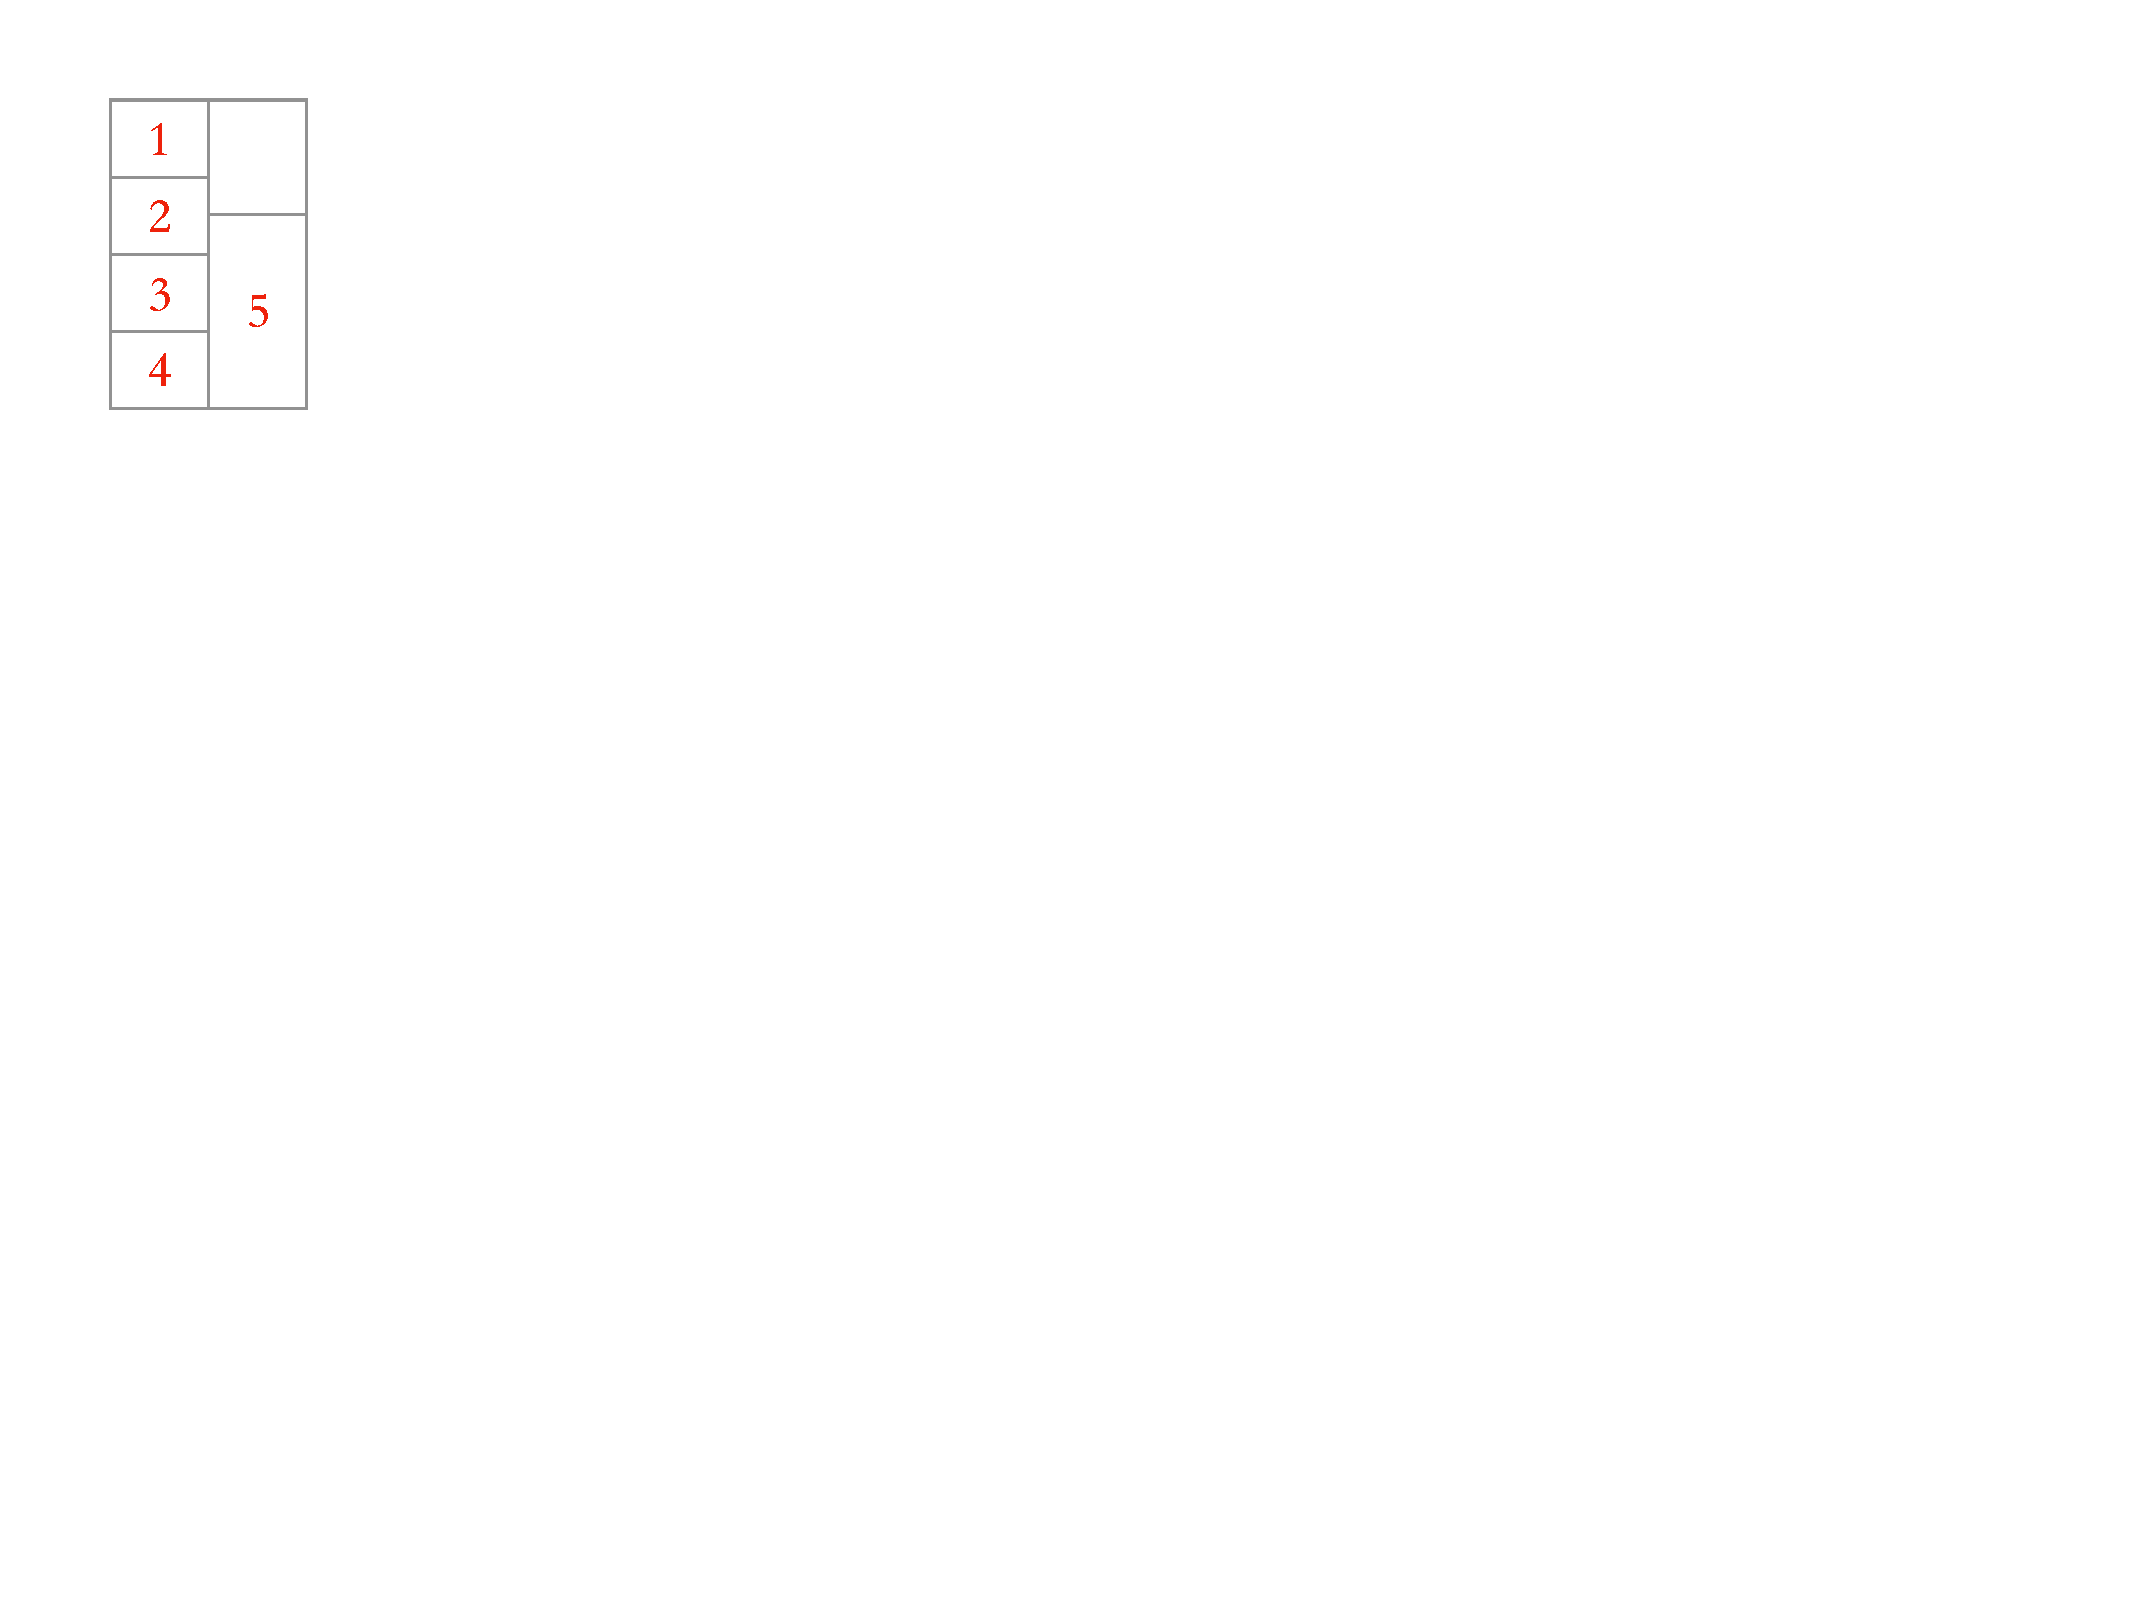
\includegraphics[width=2.5cm]{images/coverback.pdf} \\
      \textcolor{red}{\bfseries{1}} {\mbox{\color{red}\rule[-0.5mm]{1mm}{0.34cm}~~}}
        \textit{Dryopteris dickinsii} (Franchet \& Savatier) \\ 
        ~~~~~~~~~~C.Christense \\ 
        ~~~~~~~遠軸鱗毛蕨~~EN* D \\
        ~~~~~~~呂碧鳳/攝 \\
      \textcolor{red}{\bfseries{2}} {\mbox{\color{red}\rule[-0.5mm]{1mm}{0.34cm}~~}}
        \textit{Lilium speciosum} Thunb. var. \textit{oriosoides} \\ 
        ~~~~~~~豔紅鹿子百合~~CR C1\\
        ~~~~~~~蔡依恆/攝\\
      \textcolor{red}{\bfseries{3}} {\mbox{\color{red}\rule[-0.5mm]{1mm}{0.34cm}~~}}
        \textit{Argyreia akoensis} S.Z.Yang, P.H.Chen \& \\
        ~~~~~~~~~~G.W.Staples \\
        ~~~~~~~屏東朝顏~~CR B1a+2a; D1; D2\\
        ~~~~~~~楊勝任/攝\\
      \textcolor{red}{\bfseries{4}} {\mbox{\color{red}\rule[-0.5mm]{1mm}{0.34cm}~~}}
        \textit{Trapa japonica} Flerow \\ 
        ~~~~~~~日本菱~~CR B1ab(iii)+2ab(iii)\\
        ~~~~~~~黃朝慶/攝\\
      \textcolor{red}{\bfseries{5}} {\mbox{\color{red}\rule[-0.5mm]{1mm}{0.34cm}~~}}
        \textit{Appendicula lucbanensis} (Ames) Ames \\ 
        ~~~~~~~多枝竹節蘭~~CR B2ab(iii)\\
        ~~~~~~~許天銓/攝~
        }
      } \\ 
      \textbf{Authors}           & Editorial Committee of the Red List of Taiwan Plants  & \\
      \textbf{Editorial Committee} & 2008--2010: Wang, Jenn-Che (coordinator);
                                     Chang, Ho-Ming;
                                     Chiou, Wen-Liang;
                                     Hsieh, Chang-Fu;
                                     Hsu, Tsai-Wen;
                                     Kuo, Chang-Sheng;
                                     Liu, Ho-Yih;
                                     Peng, Ching-I;
                                     Yang, Kuoh-Cheng  & \\
                                   &  2017: Liu, Ho-Yih (coordinator);
                                     Chang, Ho-Ming;
                                     Chiang, Yu-Chung;
                                     Chung, Kuo-Fang;
                                     Hsieh, Tsung-Hsin; 
                                     Lin, Cheng-Tao;
                                     Liu, Yea-Chen;
                                     Tzeng, Yen-Hsueh; 
                                     Wang, Chih-Chiang  & \\
      \textbf{Executive Editors}  & Chang, Ho-Ming; Liu, Ho-Yih; Hsu, Tsai-Wen; Lin, Cheng-Tao  & \\
      \textbf{Associate Editors}  & Yang, Song-Han; Liu, Chun-Fang; Liao, Guo-Fang  & \\
      \textbf{Published by}       & Endemic Species Research Institute, COA, EY, Taiwan.
                                    Forestry Bureau, Council of Agriculture, COA, EY, Taiwan.
                                    Taiwan Society of Plant Systematics  & \\
      \textbf{Address}            & No. 1, Ming-Shen East Road, Jiji Township, Nantou County, 55244, Taiwan  & \\
      \textbf{Published Date}     & December 2017  & \\
      \textbf{ISBN}               & 978-986-05-5021-4  & \\
      \textbf{GPN}                & 1010602773  & \\
      \textbf{Download URL}  & \href{http://tesri.tesri.gov.tw}{Taiwan Endemic Species Research Institute URL:http://tesri.tesri.gov.tw}  & \\
                                  & \href{http://www.tsps.org.tw}{Taiwan Society of Plant Systematics URL: http://www.tsps.org.tw}  & \\
      \textbf{Price}              & NTD 350  & \\
      \textbf{License}            & \href{https://creativecommons.org/licenses/by/4.0}{Creative Commons Attribution 4.0 International License}.
                                     You must give appropriate credit, provide a link to the license,
                                     and indicate if changes were made. You may do so in any reasonable manner,
                                     but not in any way that suggests the licensor endorses you or your use.  & \\
  \end{tabular}
  }
  \begin{tabular}{p{2.5cm}p{3cm}p{1.0cm}p{1.6cm}p{1.6cm}}
    & 
\includegraphics[width=10em]{images/ccby40.png} & &
    
\includegraphics[width=1.4cm]{images/tesri.png} &
    
\includegraphics[width=1.4cm]{images/tsps.png} \\
  \end{tabular}

\end{table}
%\clearpage
%\thispagestyle{empty}
%\hfill
%\vfill
%{\raggedright\vfill
%   \hfill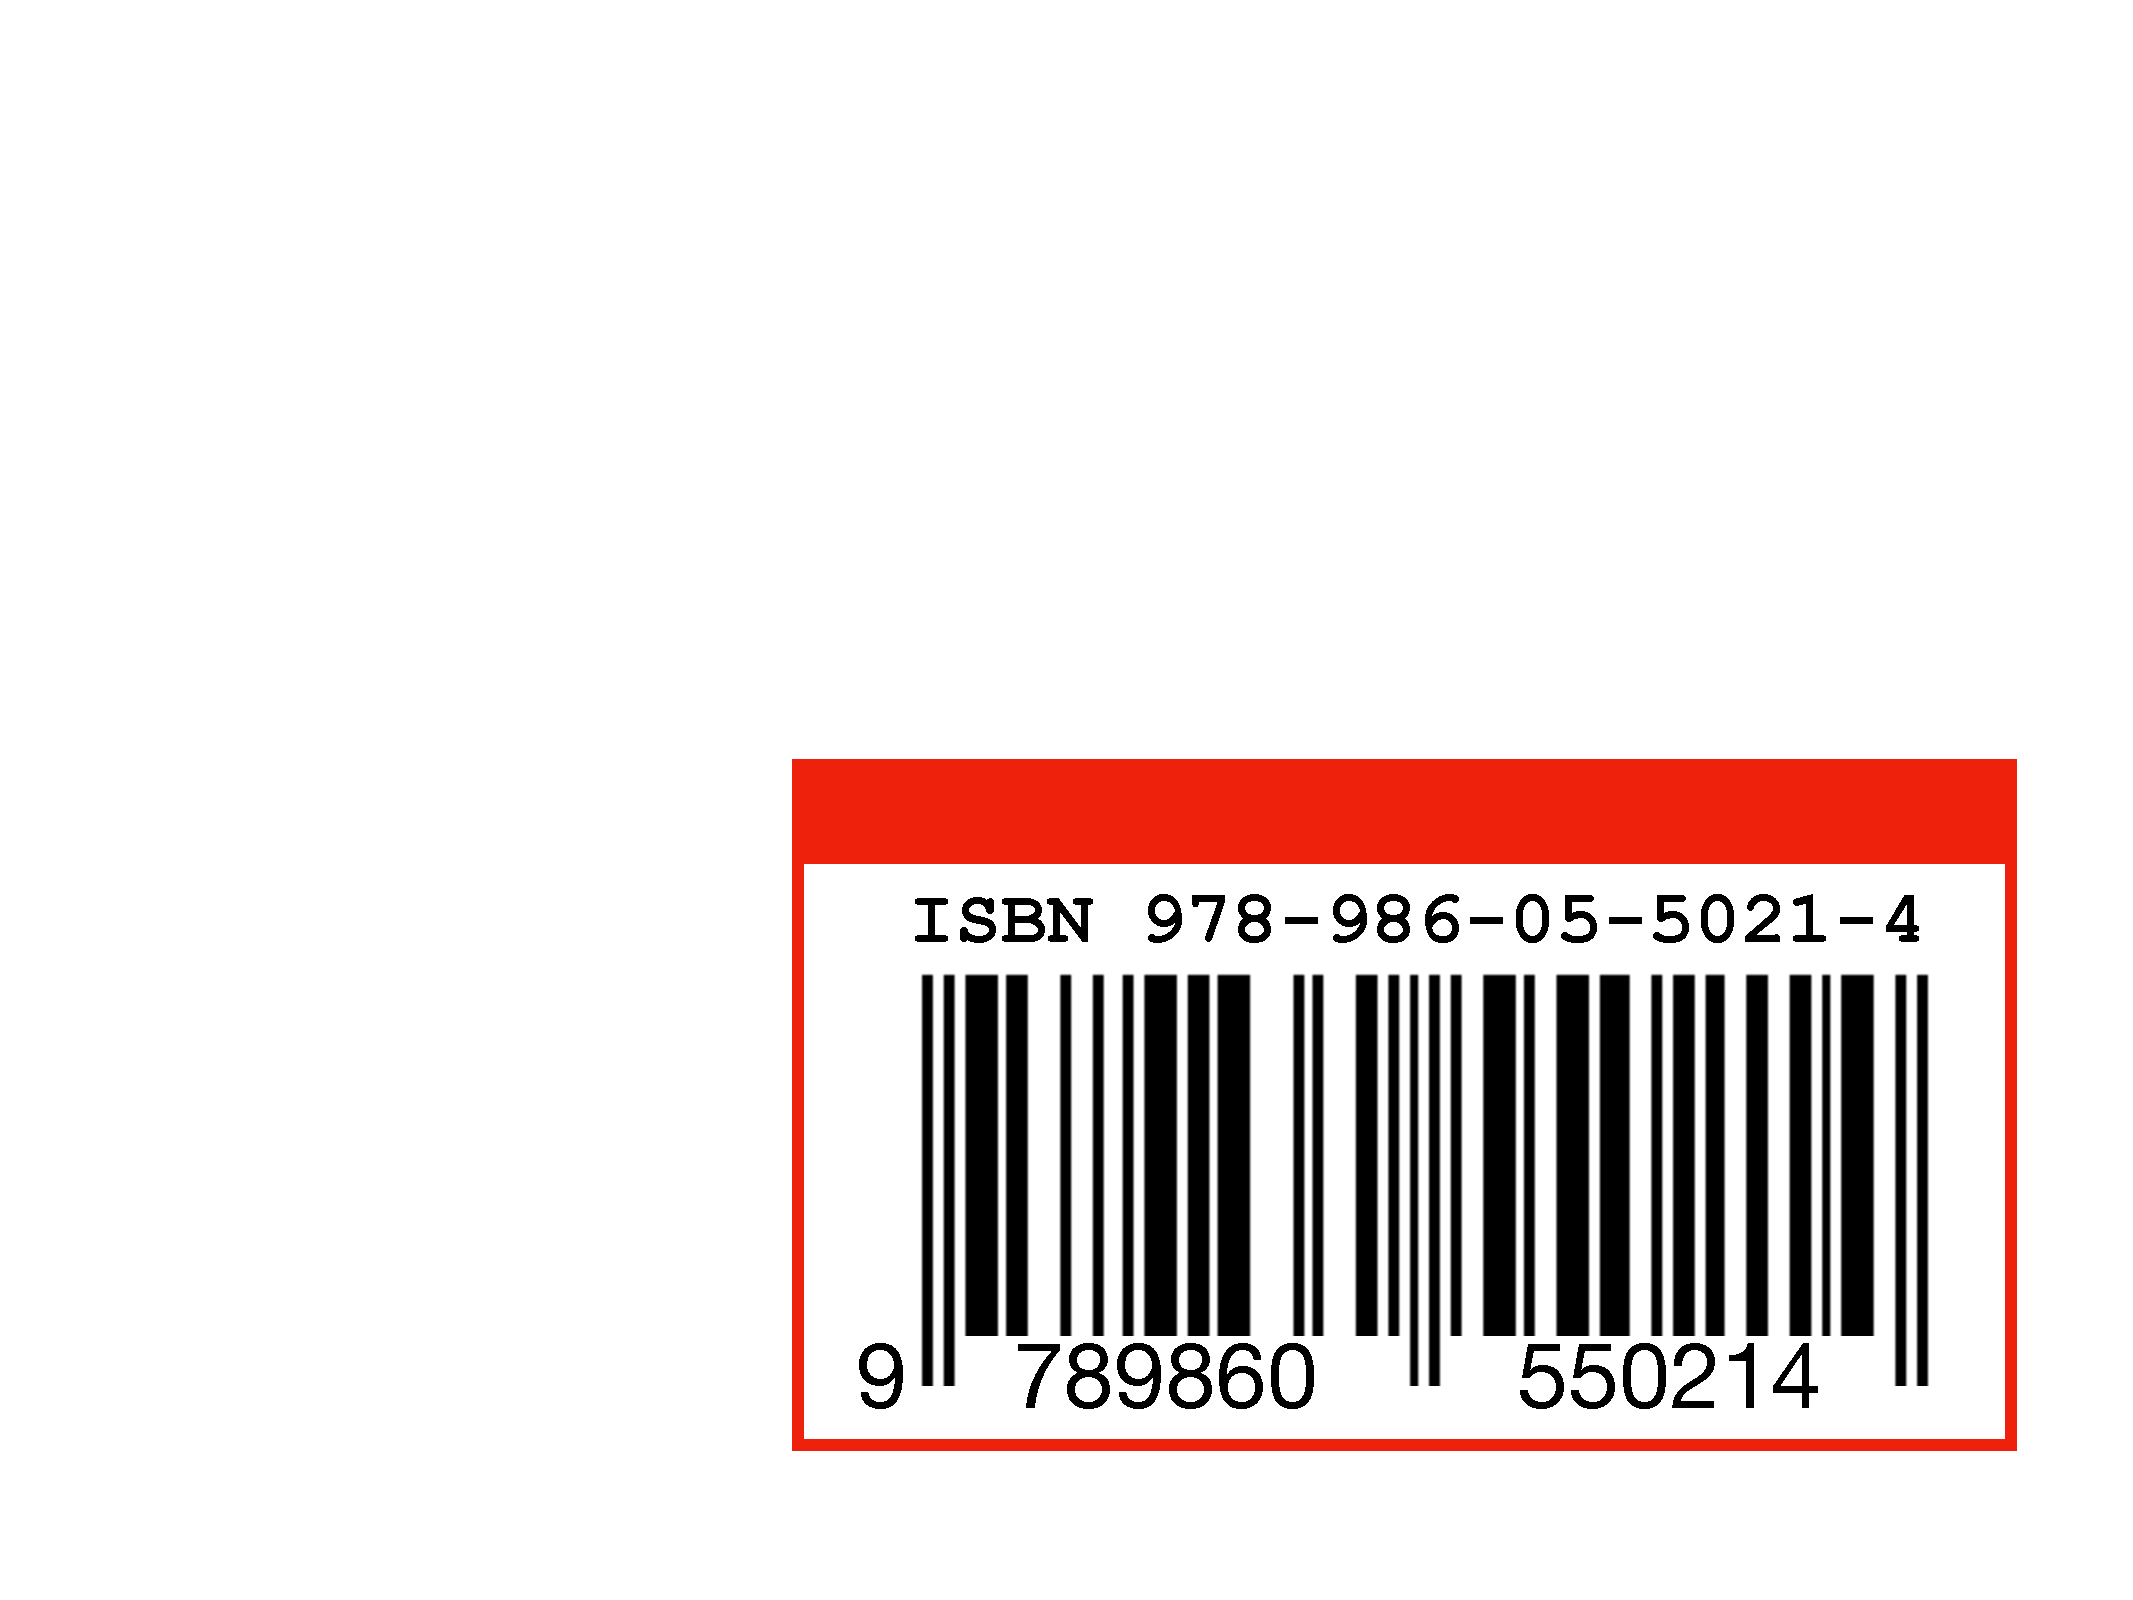
\includegraphics[width=5cm]{images/isbn_final.pdf}
%}

\end{document}
